%%%%%%%%%%%%%%%%%%%%%%%%%%%%%%%%%%%%%%%%%%%%%%%%%%%%%%%%%%%%%%%%%%%%%%%%
%% $Id$
%%%%%%%%%%%%%%%%%%%%%%%%%%%%%%%%%%%%%%%%%%%%%%%%%%%%%%%%%%%%%%%%%%%%%%%%
% This file and the files in this directory and its subdirectories
% are intended to test several parts of the TeXnicCenter-system.
%
% Copyright (C) 2002-$CurrentYear$ ToolsCenter

% Their main purpose is to reproduce several bugs or behaviours coming
% up from missing features. They are neither a good starting point for
% working with TeX nor with the TeXnicCenter-system. If you use them,
% you do this on your own risk. They come WITHOUT ANY WARRANTY;
% without even the implied warranty of MERCHANTABILITY or
% FITNESS FOR A PARTICULAR PURPOSE.
%
% Anything below the "end of prolog"-line is for testing purposes only
% and does not reflect the opinions of the author(s) and is not meant
% to be a statement at all; it is even not said to be true or reliable.
%
% If you have further questions or if you want to support
% further TeXnicCenter development, visit the TeXnicCenter-homepage
%
%     http://www.ToolsCenter.org
%
% end of prolog %%%%%%%%%%%%%%%%%%%%%%%%%%%%%%%%%%%%%%%%%%%%%%%%%%%%%%%%

%%%%%%%%%%%%%%%%%%%%%%%%%%%%%%%%%%%%%%%%%%%%%%%%%%%%%%%%%%%%%
%% HEADER
%%%%%%%%%%%%%%%%%%%%%%%%%%%%%%%%%%%%%%%%%%%%%%%%%%%%%%%%%%%%%
\documentclass[a4paper,oneside,10pt]{report}
\usepackage[draft]{graphicx}
\usepackage[latin1]{inputenc}

%%%%%%%%%%%%%%%%%%%%%%%%%%%%%%%%%%%%%%%%%%%%%%%%%%%%%%%%%%%%%
%% COMMENTS
%%%%%%%%%%%%%%%%%%%%%%%%%%%%%%%%%%%%%%%%%%%%%%%%%%%%%%%%%%%%%
%
%
%
%
%%%%%%%%%%%%%%%%%%%%%%%%%%%%%%%%%%%%%%%%%%%%%%%%%%%%%%%%%%%%%

%%%%%%%%%%%%%%%%%%%%%%%%%%%%%%%%%%%%%%%%%%%%%%%%%%%%%%%%%%%%%
%% DOCUMENT
%%%%%%%%%%%%%%%%%%%%%%%%%%%%%%%%%%%%%%%%%%%%%%%%%%%%%%%%%%%%%
\begin{document}


%%%%%%%%%%%%%%%%%%%%%%%%%%%%%%%%
% Stressing with 

%%%%%%%%%%%%%%%%%%%%%%%%%%%%%%%%%%%%%%%%%%%%%%%%%%%%%%%%%%%%%%%%%%%%%%%%
%% $Id$
%%%%%%%%%%%%%%%%%%%%%%%%%%%%%%%%%%%%%%%%%%%%%%%%%%%%%%%%%%%%%%%%%%%%%%%%
% This file and the files in this directory and its subdirectories
% are intended to test several parts of the TeXnicCenter-system.
%
% Copyright (C) 2002-$CurrentYear$ ToolsCenter

% Their main purpose is to reproduce several bugs or behaviours coming
% up from missing features. They are neither a good starting point for
% working with TeX nor with the TeXnicCenter-system. If you use them,
% you do this on your own risk. They come WITHOUT ANY WARRANTY;
% without even the implied warranty of MERCHANTABILITY or
% FITNESS FOR A PARTICULAR PURPOSE.
%
% Anything below the "end of prolog"-line is for testing purposes only
% and does not reflect the opinions of the author(s) and is not meant
% to be a statement at all; it is even not said to be true or reliable.
%
% If you have further questions or if you want to support
% further TeXnicCenter development, visit the TeXnicCenter-homepage
%
%     http://www.ToolsCenter.org
%
% end of prolog %%%%%%%%%%%%%%%%%%%%%%%%%%%%%%%%%%%%%%%%%%%%%%%%%%%%%%%%

\part{Stress Sectioning Part I}

\chapter{Chapter}

\section{Section}

\begin{footnotesize}
\input{../../../TeXnicCenter/License.txt}
\end{footnotesize}

\subsection{SubSection}

\subsection{SubSection}

\subsubsection{SubSubSection}
\subsubsection{SubSubSection}

\subsection{SubSection}
\subsubsection{SubSubSection}


\section{Section}



\chapter{Chapter}

\section{Section}

\subsection{SubSection}

\subsection{SubSection}



\chapter{Chapter}

\section{Section}
\section{Section}
\section{Section}

\subsection{SubSection}
\subsubsection{SubSubSection}

\subsection{SubSection}
\subsubsection{SubSubSection}

\section{Section}

%%%%%%%%%%%%%%%%%%%%%%%%%%%%%%%%%%%%%%%%%%%%%%%%%%%%%%%%%%%%%%%%%%%%%%%%
%% $Id$
%%%%%%%%%%%%%%%%%%%%%%%%%%%%%%%%%%%%%%%%%%%%%%%%%%%%%%%%%%%%%%%%%%%%%%%%
% This file and the files in this directory and its subdirectories
% are intended to test several parts of the TeXnicCenter-system.
%
% Copyright (C) 2002-$CurrentYear$ ToolsCenter

% Their main purpose is to reproduce several bugs or behaviours coming
% up from missing features. They are neither a good starting point for
% working with TeX nor with the TeXnicCenter-system. If you use them,
% you do this on your own risk. They come WITHOUT ANY WARRANTY;
% without even the implied warranty of MERCHANTABILITY or
% FITNESS FOR A PARTICULAR PURPOSE.
%
% Anything below the "end of prolog"-line is for testing purposes only
% and does not reflect the opinions of the author(s) and is not meant
% to be a statement at all; it is even not said to be true or reliable.
%
% If you have further questions or if you want to support
% further TeXnicCenter development, visit the TeXnicCenter-homepage
%
%     http://www.ToolsCenter.org
%
% end of prolog %%%%%%%%%%%%%%%%%%%%%%%%%%%%%%%%%%%%%%%%%%%%%%%%%%%%%%%%

% 1000 Tables

%%%%%%%%%%%%%%%%%%%%%%%%%%%%%%%%%%%%%%%%%%%%%%%%%%%%%%%%%%%%%%%%%%%%%%%%
%% $Id$
%%%%%%%%%%%%%%%%%%%%%%%%%%%%%%%%%%%%%%%%%%%%%%%%%%%%%%%%%%%%%%%%%%%%%%%%
% This file and the files in this directory and its subdirectories
% are intended to test several parts of the TeXnicCenter-system.
%
% Copyright (C) 2002-$CurrentYear$ ToolsCenter

% Their main purpose is to reproduce several bugs or behaviours coming
% up from missing features. They are neither a good starting point for
% working with TeX nor with the TeXnicCenter-system. If you use them,
% you do this on your own risk. They come WITHOUT ANY WARRANTY;
% without even the implied warranty of MERCHANTABILITY or
% FITNESS FOR A PARTICULAR PURPOSE.
%
% Anything below the "end of prolog"-line is for testing purposes only
% and does not reflect the opinions of the author(s) and is not meant
% to be a statement at all; it is even not said to be true or reliable.
%
% If you have further questions or if you want to support
% further TeXnicCenter development, visit the TeXnicCenter-homepage
%
%     http://www.ToolsCenter.org
%
% end of prolog %%%%%%%%%%%%%%%%%%%%%%%%%%%%%%%%%%%%%%%%%%%%%%%%%%%%%%%%

% 25 Tables

\begin{table}
	\begin{center}\footnotesize
		\begin{tabular}{||c|c||}
			\hline
			This is a table & to test the StructureParser.\\
			\hline
			%%%%%%%%%%%%%%%%%%%%%%%%%%%%%%%%%%%%%%%%%%%%%%%%%%%%%%%%%%%%%%%%%%%%%%%%
%% $Id$
%%%%%%%%%%%%%%%%%%%%%%%%%%%%%%%%%%%%%%%%%%%%%%%%%%%%%%%%%%%%%%%%%%%%%%%%
% This file and the files in this directory and its subdirectories
% are intended to test several parts of the TeXnicCenter-system.
%
% Copyright (C) 2002-$CurrentYear$ ToolsCenter

% Their main purpose is to reproduce several bugs or behaviours coming
% up from missing features. They are neither a good starting point for
% working with TeX nor with the TeXnicCenter-system. If you use them,
% you do this on your own risk. They come WITHOUT ANY WARRANTY;
% without even the implied warranty of MERCHANTABILITY or
% FITNESS FOR A PARTICULAR PURPOSE.
%
% Anything below the "end of prolog"-line is for testing purposes only
% and does not reflect the opinions of the author(s) and is not meant
% to be a statement at all; it is even not said to be true or reliable.
%
% If you have further questions or if you want to support
% further TeXnicCenter development, visit the TeXnicCenter-homepage
%
%     http://www.ToolsCenter.org
%
% end of prolog %%%%%%%%%%%%%%%%%%%%%%%%%%%%%%%%%%%%%%%%%%%%%%%%%%%%%%%%

% About 25 Table entries
The licenses for most & software are designed to take away\\
your freedom to & share and change it.\\
By contrast, the & GNU General Public License is intended\\
to guarantee your freedom & to share and change free software\\
--to make sure the & software is free for all its users.\\
This General Public License & applies to most of the Free Software Foundation's software\\
and to & any other program\\
whose authors & commit to using it.\\
(Some other Free Software Foundation & software\\
is covered by the & GNU Library General Public License instead.)\\
You can apply it & to your programs, too.\\
 & \\
\hline
 & \\
The licenses for most & software are designed to take away\\
your freedom to & share and change it.\\
By contrast, the & GNU General Public License is intended\\
to guarantee your freedom & to share and change free software\\
--to make sure the & software is free for all its users.\\
This General Public License & applies to most of the Free Software Foundation's software\\
and to & any other program\\
whose authors & commit to using it.\\
(Some other Free Software Foundation & software\\
is covered by the & GNU Library General Public License instead.)\\
You can apply it & to your programs, too.\\
 & \\
\hline
 & \\
TeXnicCenter is distributed & under the terms of the GPL.\\

			\hline
		\end{tabular}
	\end{center}
	\caption{A Table to test the StructureParser}
\end{table}

\begin{table}
	\begin{center}\footnotesize
		\begin{tabular}{||c|c||}
			\hline
			This is a table & to test the StructureParser.\\
			\hline
			%%%%%%%%%%%%%%%%%%%%%%%%%%%%%%%%%%%%%%%%%%%%%%%%%%%%%%%%%%%%%%%%%%%%%%%%
%% $Id$
%%%%%%%%%%%%%%%%%%%%%%%%%%%%%%%%%%%%%%%%%%%%%%%%%%%%%%%%%%%%%%%%%%%%%%%%
% This file and the files in this directory and its subdirectories
% are intended to test several parts of the TeXnicCenter-system.
%
% Copyright (C) 2002-$CurrentYear$ ToolsCenter

% Their main purpose is to reproduce several bugs or behaviours coming
% up from missing features. They are neither a good starting point for
% working with TeX nor with the TeXnicCenter-system. If you use them,
% you do this on your own risk. They come WITHOUT ANY WARRANTY;
% without even the implied warranty of MERCHANTABILITY or
% FITNESS FOR A PARTICULAR PURPOSE.
%
% Anything below the "end of prolog"-line is for testing purposes only
% and does not reflect the opinions of the author(s) and is not meant
% to be a statement at all; it is even not said to be true or reliable.
%
% If you have further questions or if you want to support
% further TeXnicCenter development, visit the TeXnicCenter-homepage
%
%     http://www.ToolsCenter.org
%
% end of prolog %%%%%%%%%%%%%%%%%%%%%%%%%%%%%%%%%%%%%%%%%%%%%%%%%%%%%%%%

% About 25 Table entries
The licenses for most & software are designed to take away\\
your freedom to & share and change it.\\
By contrast, the & GNU General Public License is intended\\
to guarantee your freedom & to share and change free software\\
--to make sure the & software is free for all its users.\\
This General Public License & applies to most of the Free Software Foundation's software\\
and to & any other program\\
whose authors & commit to using it.\\
(Some other Free Software Foundation & software\\
is covered by the & GNU Library General Public License instead.)\\
You can apply it & to your programs, too.\\
 & \\
\hline
 & \\
The licenses for most & software are designed to take away\\
your freedom to & share and change it.\\
By contrast, the & GNU General Public License is intended\\
to guarantee your freedom & to share and change free software\\
--to make sure the & software is free for all its users.\\
This General Public License & applies to most of the Free Software Foundation's software\\
and to & any other program\\
whose authors & commit to using it.\\
(Some other Free Software Foundation & software\\
is covered by the & GNU Library General Public License instead.)\\
You can apply it & to your programs, too.\\
 & \\
\hline
 & \\
TeXnicCenter is distributed & under the terms of the GPL.\\

			\hline
		\end{tabular}
	\end{center}
	\caption{A Table to test the StructureParser}
\end{table}

\clearpage

\begin{table}
	\begin{center}\footnotesize
		\begin{tabular}{||c|c||}
			\hline
			This is a table & to test the StructureParser.\\
			\hline
			%%%%%%%%%%%%%%%%%%%%%%%%%%%%%%%%%%%%%%%%%%%%%%%%%%%%%%%%%%%%%%%%%%%%%%%%
%% $Id$
%%%%%%%%%%%%%%%%%%%%%%%%%%%%%%%%%%%%%%%%%%%%%%%%%%%%%%%%%%%%%%%%%%%%%%%%
% This file and the files in this directory and its subdirectories
% are intended to test several parts of the TeXnicCenter-system.
%
% Copyright (C) 2002-$CurrentYear$ ToolsCenter

% Their main purpose is to reproduce several bugs or behaviours coming
% up from missing features. They are neither a good starting point for
% working with TeX nor with the TeXnicCenter-system. If you use them,
% you do this on your own risk. They come WITHOUT ANY WARRANTY;
% without even the implied warranty of MERCHANTABILITY or
% FITNESS FOR A PARTICULAR PURPOSE.
%
% Anything below the "end of prolog"-line is for testing purposes only
% and does not reflect the opinions of the author(s) and is not meant
% to be a statement at all; it is even not said to be true or reliable.
%
% If you have further questions or if you want to support
% further TeXnicCenter development, visit the TeXnicCenter-homepage
%
%     http://www.ToolsCenter.org
%
% end of prolog %%%%%%%%%%%%%%%%%%%%%%%%%%%%%%%%%%%%%%%%%%%%%%%%%%%%%%%%

% About 25 Table entries
The licenses for most & software are designed to take away\\
your freedom to & share and change it.\\
By contrast, the & GNU General Public License is intended\\
to guarantee your freedom & to share and change free software\\
--to make sure the & software is free for all its users.\\
This General Public License & applies to most of the Free Software Foundation's software\\
and to & any other program\\
whose authors & commit to using it.\\
(Some other Free Software Foundation & software\\
is covered by the & GNU Library General Public License instead.)\\
You can apply it & to your programs, too.\\
 & \\
\hline
 & \\
The licenses for most & software are designed to take away\\
your freedom to & share and change it.\\
By contrast, the & GNU General Public License is intended\\
to guarantee your freedom & to share and change free software\\
--to make sure the & software is free for all its users.\\
This General Public License & applies to most of the Free Software Foundation's software\\
and to & any other program\\
whose authors & commit to using it.\\
(Some other Free Software Foundation & software\\
is covered by the & GNU Library General Public License instead.)\\
You can apply it & to your programs, too.\\
 & \\
\hline
 & \\
TeXnicCenter is distributed & under the terms of the GPL.\\

			\hline
		\end{tabular}
	\end{center}
	\caption{A Table to test the StructureParser}
\end{table}

\begin{table}
	\begin{center}\footnotesize
		\begin{tabular}{||c|c||}
			\hline
			This is a table & to test the StructureParser.\\
			\hline
			%%%%%%%%%%%%%%%%%%%%%%%%%%%%%%%%%%%%%%%%%%%%%%%%%%%%%%%%%%%%%%%%%%%%%%%%
%% $Id$
%%%%%%%%%%%%%%%%%%%%%%%%%%%%%%%%%%%%%%%%%%%%%%%%%%%%%%%%%%%%%%%%%%%%%%%%
% This file and the files in this directory and its subdirectories
% are intended to test several parts of the TeXnicCenter-system.
%
% Copyright (C) 2002-$CurrentYear$ ToolsCenter

% Their main purpose is to reproduce several bugs or behaviours coming
% up from missing features. They are neither a good starting point for
% working with TeX nor with the TeXnicCenter-system. If you use them,
% you do this on your own risk. They come WITHOUT ANY WARRANTY;
% without even the implied warranty of MERCHANTABILITY or
% FITNESS FOR A PARTICULAR PURPOSE.
%
% Anything below the "end of prolog"-line is for testing purposes only
% and does not reflect the opinions of the author(s) and is not meant
% to be a statement at all; it is even not said to be true or reliable.
%
% If you have further questions or if you want to support
% further TeXnicCenter development, visit the TeXnicCenter-homepage
%
%     http://www.ToolsCenter.org
%
% end of prolog %%%%%%%%%%%%%%%%%%%%%%%%%%%%%%%%%%%%%%%%%%%%%%%%%%%%%%%%

% About 25 Table entries
The licenses for most & software are designed to take away\\
your freedom to & share and change it.\\
By contrast, the & GNU General Public License is intended\\
to guarantee your freedom & to share and change free software\\
--to make sure the & software is free for all its users.\\
This General Public License & applies to most of the Free Software Foundation's software\\
and to & any other program\\
whose authors & commit to using it.\\
(Some other Free Software Foundation & software\\
is covered by the & GNU Library General Public License instead.)\\
You can apply it & to your programs, too.\\
 & \\
\hline
 & \\
The licenses for most & software are designed to take away\\
your freedom to & share and change it.\\
By contrast, the & GNU General Public License is intended\\
to guarantee your freedom & to share and change free software\\
--to make sure the & software is free for all its users.\\
This General Public License & applies to most of the Free Software Foundation's software\\
and to & any other program\\
whose authors & commit to using it.\\
(Some other Free Software Foundation & software\\
is covered by the & GNU Library General Public License instead.)\\
You can apply it & to your programs, too.\\
 & \\
\hline
 & \\
TeXnicCenter is distributed & under the terms of the GPL.\\

			\hline
		\end{tabular}
	\end{center}
	\caption{A Table to test the StructureParser}
\end{table}

\clearpage

\begin{table}
	\begin{center}\footnotesize
		\begin{tabular}{||c|c||}
			\hline
			This is a table & to test the StructureParser.\\
			\hline
			%%%%%%%%%%%%%%%%%%%%%%%%%%%%%%%%%%%%%%%%%%%%%%%%%%%%%%%%%%%%%%%%%%%%%%%%
%% $Id$
%%%%%%%%%%%%%%%%%%%%%%%%%%%%%%%%%%%%%%%%%%%%%%%%%%%%%%%%%%%%%%%%%%%%%%%%
% This file and the files in this directory and its subdirectories
% are intended to test several parts of the TeXnicCenter-system.
%
% Copyright (C) 2002-$CurrentYear$ ToolsCenter

% Their main purpose is to reproduce several bugs or behaviours coming
% up from missing features. They are neither a good starting point for
% working with TeX nor with the TeXnicCenter-system. If you use them,
% you do this on your own risk. They come WITHOUT ANY WARRANTY;
% without even the implied warranty of MERCHANTABILITY or
% FITNESS FOR A PARTICULAR PURPOSE.
%
% Anything below the "end of prolog"-line is for testing purposes only
% and does not reflect the opinions of the author(s) and is not meant
% to be a statement at all; it is even not said to be true or reliable.
%
% If you have further questions or if you want to support
% further TeXnicCenter development, visit the TeXnicCenter-homepage
%
%     http://www.ToolsCenter.org
%
% end of prolog %%%%%%%%%%%%%%%%%%%%%%%%%%%%%%%%%%%%%%%%%%%%%%%%%%%%%%%%

% About 25 Table entries
The licenses for most & software are designed to take away\\
your freedom to & share and change it.\\
By contrast, the & GNU General Public License is intended\\
to guarantee your freedom & to share and change free software\\
--to make sure the & software is free for all its users.\\
This General Public License & applies to most of the Free Software Foundation's software\\
and to & any other program\\
whose authors & commit to using it.\\
(Some other Free Software Foundation & software\\
is covered by the & GNU Library General Public License instead.)\\
You can apply it & to your programs, too.\\
 & \\
\hline
 & \\
The licenses for most & software are designed to take away\\
your freedom to & share and change it.\\
By contrast, the & GNU General Public License is intended\\
to guarantee your freedom & to share and change free software\\
--to make sure the & software is free for all its users.\\
This General Public License & applies to most of the Free Software Foundation's software\\
and to & any other program\\
whose authors & commit to using it.\\
(Some other Free Software Foundation & software\\
is covered by the & GNU Library General Public License instead.)\\
You can apply it & to your programs, too.\\
 & \\
\hline
 & \\
TeXnicCenter is distributed & under the terms of the GPL.\\

			\hline
		\end{tabular}
	\end{center}
	\caption{A Table to test the StructureParser}
\end{table}

\begin{table}
	\begin{center}\footnotesize
		\begin{tabular}{||c|c||}
			\hline
			This is a table & to test the StructureParser.\\
			\hline
			%%%%%%%%%%%%%%%%%%%%%%%%%%%%%%%%%%%%%%%%%%%%%%%%%%%%%%%%%%%%%%%%%%%%%%%%
%% $Id$
%%%%%%%%%%%%%%%%%%%%%%%%%%%%%%%%%%%%%%%%%%%%%%%%%%%%%%%%%%%%%%%%%%%%%%%%
% This file and the files in this directory and its subdirectories
% are intended to test several parts of the TeXnicCenter-system.
%
% Copyright (C) 2002-$CurrentYear$ ToolsCenter

% Their main purpose is to reproduce several bugs or behaviours coming
% up from missing features. They are neither a good starting point for
% working with TeX nor with the TeXnicCenter-system. If you use them,
% you do this on your own risk. They come WITHOUT ANY WARRANTY;
% without even the implied warranty of MERCHANTABILITY or
% FITNESS FOR A PARTICULAR PURPOSE.
%
% Anything below the "end of prolog"-line is for testing purposes only
% and does not reflect the opinions of the author(s) and is not meant
% to be a statement at all; it is even not said to be true or reliable.
%
% If you have further questions or if you want to support
% further TeXnicCenter development, visit the TeXnicCenter-homepage
%
%     http://www.ToolsCenter.org
%
% end of prolog %%%%%%%%%%%%%%%%%%%%%%%%%%%%%%%%%%%%%%%%%%%%%%%%%%%%%%%%

% About 25 Table entries
The licenses for most & software are designed to take away\\
your freedom to & share and change it.\\
By contrast, the & GNU General Public License is intended\\
to guarantee your freedom & to share and change free software\\
--to make sure the & software is free for all its users.\\
This General Public License & applies to most of the Free Software Foundation's software\\
and to & any other program\\
whose authors & commit to using it.\\
(Some other Free Software Foundation & software\\
is covered by the & GNU Library General Public License instead.)\\
You can apply it & to your programs, too.\\
 & \\
\hline
 & \\
The licenses for most & software are designed to take away\\
your freedom to & share and change it.\\
By contrast, the & GNU General Public License is intended\\
to guarantee your freedom & to share and change free software\\
--to make sure the & software is free for all its users.\\
This General Public License & applies to most of the Free Software Foundation's software\\
and to & any other program\\
whose authors & commit to using it.\\
(Some other Free Software Foundation & software\\
is covered by the & GNU Library General Public License instead.)\\
You can apply it & to your programs, too.\\
 & \\
\hline
 & \\
TeXnicCenter is distributed & under the terms of the GPL.\\

			\hline
		\end{tabular}
	\end{center}
	\caption{A Table to test the StructureParser}
\end{table}

\clearpage

\begin{table}
	\begin{center}\footnotesize
		\begin{tabular}{||c|c||}
			\hline
			This is a table & to test the StructureParser.\\
			\hline
			%%%%%%%%%%%%%%%%%%%%%%%%%%%%%%%%%%%%%%%%%%%%%%%%%%%%%%%%%%%%%%%%%%%%%%%%
%% $Id$
%%%%%%%%%%%%%%%%%%%%%%%%%%%%%%%%%%%%%%%%%%%%%%%%%%%%%%%%%%%%%%%%%%%%%%%%
% This file and the files in this directory and its subdirectories
% are intended to test several parts of the TeXnicCenter-system.
%
% Copyright (C) 2002-$CurrentYear$ ToolsCenter

% Their main purpose is to reproduce several bugs or behaviours coming
% up from missing features. They are neither a good starting point for
% working with TeX nor with the TeXnicCenter-system. If you use them,
% you do this on your own risk. They come WITHOUT ANY WARRANTY;
% without even the implied warranty of MERCHANTABILITY or
% FITNESS FOR A PARTICULAR PURPOSE.
%
% Anything below the "end of prolog"-line is for testing purposes only
% and does not reflect the opinions of the author(s) and is not meant
% to be a statement at all; it is even not said to be true or reliable.
%
% If you have further questions or if you want to support
% further TeXnicCenter development, visit the TeXnicCenter-homepage
%
%     http://www.ToolsCenter.org
%
% end of prolog %%%%%%%%%%%%%%%%%%%%%%%%%%%%%%%%%%%%%%%%%%%%%%%%%%%%%%%%

% About 25 Table entries
The licenses for most & software are designed to take away\\
your freedom to & share and change it.\\
By contrast, the & GNU General Public License is intended\\
to guarantee your freedom & to share and change free software\\
--to make sure the & software is free for all its users.\\
This General Public License & applies to most of the Free Software Foundation's software\\
and to & any other program\\
whose authors & commit to using it.\\
(Some other Free Software Foundation & software\\
is covered by the & GNU Library General Public License instead.)\\
You can apply it & to your programs, too.\\
 & \\
\hline
 & \\
The licenses for most & software are designed to take away\\
your freedom to & share and change it.\\
By contrast, the & GNU General Public License is intended\\
to guarantee your freedom & to share and change free software\\
--to make sure the & software is free for all its users.\\
This General Public License & applies to most of the Free Software Foundation's software\\
and to & any other program\\
whose authors & commit to using it.\\
(Some other Free Software Foundation & software\\
is covered by the & GNU Library General Public License instead.)\\
You can apply it & to your programs, too.\\
 & \\
\hline
 & \\
TeXnicCenter is distributed & under the terms of the GPL.\\

			\hline
		\end{tabular}
	\end{center}
	\caption{A Table to test the StructureParser}
\end{table}

\begin{table}
	\begin{center}\footnotesize
		\begin{tabular}{||c|c||}
			\hline
			This is a table & to test the StructureParser.\\
			\hline
			%%%%%%%%%%%%%%%%%%%%%%%%%%%%%%%%%%%%%%%%%%%%%%%%%%%%%%%%%%%%%%%%%%%%%%%%
%% $Id$
%%%%%%%%%%%%%%%%%%%%%%%%%%%%%%%%%%%%%%%%%%%%%%%%%%%%%%%%%%%%%%%%%%%%%%%%
% This file and the files in this directory and its subdirectories
% are intended to test several parts of the TeXnicCenter-system.
%
% Copyright (C) 2002-$CurrentYear$ ToolsCenter

% Their main purpose is to reproduce several bugs or behaviours coming
% up from missing features. They are neither a good starting point for
% working with TeX nor with the TeXnicCenter-system. If you use them,
% you do this on your own risk. They come WITHOUT ANY WARRANTY;
% without even the implied warranty of MERCHANTABILITY or
% FITNESS FOR A PARTICULAR PURPOSE.
%
% Anything below the "end of prolog"-line is for testing purposes only
% and does not reflect the opinions of the author(s) and is not meant
% to be a statement at all; it is even not said to be true or reliable.
%
% If you have further questions or if you want to support
% further TeXnicCenter development, visit the TeXnicCenter-homepage
%
%     http://www.ToolsCenter.org
%
% end of prolog %%%%%%%%%%%%%%%%%%%%%%%%%%%%%%%%%%%%%%%%%%%%%%%%%%%%%%%%

% About 25 Table entries
The licenses for most & software are designed to take away\\
your freedom to & share and change it.\\
By contrast, the & GNU General Public License is intended\\
to guarantee your freedom & to share and change free software\\
--to make sure the & software is free for all its users.\\
This General Public License & applies to most of the Free Software Foundation's software\\
and to & any other program\\
whose authors & commit to using it.\\
(Some other Free Software Foundation & software\\
is covered by the & GNU Library General Public License instead.)\\
You can apply it & to your programs, too.\\
 & \\
\hline
 & \\
The licenses for most & software are designed to take away\\
your freedom to & share and change it.\\
By contrast, the & GNU General Public License is intended\\
to guarantee your freedom & to share and change free software\\
--to make sure the & software is free for all its users.\\
This General Public License & applies to most of the Free Software Foundation's software\\
and to & any other program\\
whose authors & commit to using it.\\
(Some other Free Software Foundation & software\\
is covered by the & GNU Library General Public License instead.)\\
You can apply it & to your programs, too.\\
 & \\
\hline
 & \\
TeXnicCenter is distributed & under the terms of the GPL.\\

			\hline
		\end{tabular}
	\end{center}
	\caption{A Table to test the StructureParser}
\end{table}

\clearpage

\begin{table}
	\begin{center}\footnotesize
		\begin{tabular}{||c|c||}
			\hline
			This is a table & to test the StructureParser.\\
			\hline
			%%%%%%%%%%%%%%%%%%%%%%%%%%%%%%%%%%%%%%%%%%%%%%%%%%%%%%%%%%%%%%%%%%%%%%%%
%% $Id$
%%%%%%%%%%%%%%%%%%%%%%%%%%%%%%%%%%%%%%%%%%%%%%%%%%%%%%%%%%%%%%%%%%%%%%%%
% This file and the files in this directory and its subdirectories
% are intended to test several parts of the TeXnicCenter-system.
%
% Copyright (C) 2002-$CurrentYear$ ToolsCenter

% Their main purpose is to reproduce several bugs or behaviours coming
% up from missing features. They are neither a good starting point for
% working with TeX nor with the TeXnicCenter-system. If you use them,
% you do this on your own risk. They come WITHOUT ANY WARRANTY;
% without even the implied warranty of MERCHANTABILITY or
% FITNESS FOR A PARTICULAR PURPOSE.
%
% Anything below the "end of prolog"-line is for testing purposes only
% and does not reflect the opinions of the author(s) and is not meant
% to be a statement at all; it is even not said to be true or reliable.
%
% If you have further questions or if you want to support
% further TeXnicCenter development, visit the TeXnicCenter-homepage
%
%     http://www.ToolsCenter.org
%
% end of prolog %%%%%%%%%%%%%%%%%%%%%%%%%%%%%%%%%%%%%%%%%%%%%%%%%%%%%%%%

% About 25 Table entries
The licenses for most & software are designed to take away\\
your freedom to & share and change it.\\
By contrast, the & GNU General Public License is intended\\
to guarantee your freedom & to share and change free software\\
--to make sure the & software is free for all its users.\\
This General Public License & applies to most of the Free Software Foundation's software\\
and to & any other program\\
whose authors & commit to using it.\\
(Some other Free Software Foundation & software\\
is covered by the & GNU Library General Public License instead.)\\
You can apply it & to your programs, too.\\
 & \\
\hline
 & \\
The licenses for most & software are designed to take away\\
your freedom to & share and change it.\\
By contrast, the & GNU General Public License is intended\\
to guarantee your freedom & to share and change free software\\
--to make sure the & software is free for all its users.\\
This General Public License & applies to most of the Free Software Foundation's software\\
and to & any other program\\
whose authors & commit to using it.\\
(Some other Free Software Foundation & software\\
is covered by the & GNU Library General Public License instead.)\\
You can apply it & to your programs, too.\\
 & \\
\hline
 & \\
TeXnicCenter is distributed & under the terms of the GPL.\\

			\hline
		\end{tabular}
	\end{center}
	\caption{A Table to test the StructureParser}
\end{table}

\begin{table}
	\begin{center}\footnotesize
		\begin{tabular}{||c|c||}
			\hline
			This is a table & to test the StructureParser.\\
			\hline
			%%%%%%%%%%%%%%%%%%%%%%%%%%%%%%%%%%%%%%%%%%%%%%%%%%%%%%%%%%%%%%%%%%%%%%%%
%% $Id$
%%%%%%%%%%%%%%%%%%%%%%%%%%%%%%%%%%%%%%%%%%%%%%%%%%%%%%%%%%%%%%%%%%%%%%%%
% This file and the files in this directory and its subdirectories
% are intended to test several parts of the TeXnicCenter-system.
%
% Copyright (C) 2002-$CurrentYear$ ToolsCenter

% Their main purpose is to reproduce several bugs or behaviours coming
% up from missing features. They are neither a good starting point for
% working with TeX nor with the TeXnicCenter-system. If you use them,
% you do this on your own risk. They come WITHOUT ANY WARRANTY;
% without even the implied warranty of MERCHANTABILITY or
% FITNESS FOR A PARTICULAR PURPOSE.
%
% Anything below the "end of prolog"-line is for testing purposes only
% and does not reflect the opinions of the author(s) and is not meant
% to be a statement at all; it is even not said to be true or reliable.
%
% If you have further questions or if you want to support
% further TeXnicCenter development, visit the TeXnicCenter-homepage
%
%     http://www.ToolsCenter.org
%
% end of prolog %%%%%%%%%%%%%%%%%%%%%%%%%%%%%%%%%%%%%%%%%%%%%%%%%%%%%%%%

% About 25 Table entries
The licenses for most & software are designed to take away\\
your freedom to & share and change it.\\
By contrast, the & GNU General Public License is intended\\
to guarantee your freedom & to share and change free software\\
--to make sure the & software is free for all its users.\\
This General Public License & applies to most of the Free Software Foundation's software\\
and to & any other program\\
whose authors & commit to using it.\\
(Some other Free Software Foundation & software\\
is covered by the & GNU Library General Public License instead.)\\
You can apply it & to your programs, too.\\
 & \\
\hline
 & \\
The licenses for most & software are designed to take away\\
your freedom to & share and change it.\\
By contrast, the & GNU General Public License is intended\\
to guarantee your freedom & to share and change free software\\
--to make sure the & software is free for all its users.\\
This General Public License & applies to most of the Free Software Foundation's software\\
and to & any other program\\
whose authors & commit to using it.\\
(Some other Free Software Foundation & software\\
is covered by the & GNU Library General Public License instead.)\\
You can apply it & to your programs, too.\\
 & \\
\hline
 & \\
TeXnicCenter is distributed & under the terms of the GPL.\\

			\hline
		\end{tabular}
	\end{center}
	\caption{A Table to test the StructureParser}
\end{table}

\clearpage

\begin{table}
	\begin{center}\footnotesize
		\begin{tabular}{||c|c||}
			\hline
			This is a table & to test the StructureParser.\\
			\hline
			%%%%%%%%%%%%%%%%%%%%%%%%%%%%%%%%%%%%%%%%%%%%%%%%%%%%%%%%%%%%%%%%%%%%%%%%
%% $Id$
%%%%%%%%%%%%%%%%%%%%%%%%%%%%%%%%%%%%%%%%%%%%%%%%%%%%%%%%%%%%%%%%%%%%%%%%
% This file and the files in this directory and its subdirectories
% are intended to test several parts of the TeXnicCenter-system.
%
% Copyright (C) 2002-$CurrentYear$ ToolsCenter

% Their main purpose is to reproduce several bugs or behaviours coming
% up from missing features. They are neither a good starting point for
% working with TeX nor with the TeXnicCenter-system. If you use them,
% you do this on your own risk. They come WITHOUT ANY WARRANTY;
% without even the implied warranty of MERCHANTABILITY or
% FITNESS FOR A PARTICULAR PURPOSE.
%
% Anything below the "end of prolog"-line is for testing purposes only
% and does not reflect the opinions of the author(s) and is not meant
% to be a statement at all; it is even not said to be true or reliable.
%
% If you have further questions or if you want to support
% further TeXnicCenter development, visit the TeXnicCenter-homepage
%
%     http://www.ToolsCenter.org
%
% end of prolog %%%%%%%%%%%%%%%%%%%%%%%%%%%%%%%%%%%%%%%%%%%%%%%%%%%%%%%%

% About 25 Table entries
The licenses for most & software are designed to take away\\
your freedom to & share and change it.\\
By contrast, the & GNU General Public License is intended\\
to guarantee your freedom & to share and change free software\\
--to make sure the & software is free for all its users.\\
This General Public License & applies to most of the Free Software Foundation's software\\
and to & any other program\\
whose authors & commit to using it.\\
(Some other Free Software Foundation & software\\
is covered by the & GNU Library General Public License instead.)\\
You can apply it & to your programs, too.\\
 & \\
\hline
 & \\
The licenses for most & software are designed to take away\\
your freedom to & share and change it.\\
By contrast, the & GNU General Public License is intended\\
to guarantee your freedom & to share and change free software\\
--to make sure the & software is free for all its users.\\
This General Public License & applies to most of the Free Software Foundation's software\\
and to & any other program\\
whose authors & commit to using it.\\
(Some other Free Software Foundation & software\\
is covered by the & GNU Library General Public License instead.)\\
You can apply it & to your programs, too.\\
 & \\
\hline
 & \\
TeXnicCenter is distributed & under the terms of the GPL.\\

			\hline
		\end{tabular}
	\end{center}
	\caption{A Table to test the StructureParser}
\end{table}

\begin{table}
	\begin{center}\footnotesize
		\begin{tabular}{||c|c||}
			\hline
			This is a table & to test the StructureParser.\\
			\hline
			%%%%%%%%%%%%%%%%%%%%%%%%%%%%%%%%%%%%%%%%%%%%%%%%%%%%%%%%%%%%%%%%%%%%%%%%
%% $Id$
%%%%%%%%%%%%%%%%%%%%%%%%%%%%%%%%%%%%%%%%%%%%%%%%%%%%%%%%%%%%%%%%%%%%%%%%
% This file and the files in this directory and its subdirectories
% are intended to test several parts of the TeXnicCenter-system.
%
% Copyright (C) 2002-$CurrentYear$ ToolsCenter

% Their main purpose is to reproduce several bugs or behaviours coming
% up from missing features. They are neither a good starting point for
% working with TeX nor with the TeXnicCenter-system. If you use them,
% you do this on your own risk. They come WITHOUT ANY WARRANTY;
% without even the implied warranty of MERCHANTABILITY or
% FITNESS FOR A PARTICULAR PURPOSE.
%
% Anything below the "end of prolog"-line is for testing purposes only
% and does not reflect the opinions of the author(s) and is not meant
% to be a statement at all; it is even not said to be true or reliable.
%
% If you have further questions or if you want to support
% further TeXnicCenter development, visit the TeXnicCenter-homepage
%
%     http://www.ToolsCenter.org
%
% end of prolog %%%%%%%%%%%%%%%%%%%%%%%%%%%%%%%%%%%%%%%%%%%%%%%%%%%%%%%%

% About 25 Table entries
The licenses for most & software are designed to take away\\
your freedom to & share and change it.\\
By contrast, the & GNU General Public License is intended\\
to guarantee your freedom & to share and change free software\\
--to make sure the & software is free for all its users.\\
This General Public License & applies to most of the Free Software Foundation's software\\
and to & any other program\\
whose authors & commit to using it.\\
(Some other Free Software Foundation & software\\
is covered by the & GNU Library General Public License instead.)\\
You can apply it & to your programs, too.\\
 & \\
\hline
 & \\
The licenses for most & software are designed to take away\\
your freedom to & share and change it.\\
By contrast, the & GNU General Public License is intended\\
to guarantee your freedom & to share and change free software\\
--to make sure the & software is free for all its users.\\
This General Public License & applies to most of the Free Software Foundation's software\\
and to & any other program\\
whose authors & commit to using it.\\
(Some other Free Software Foundation & software\\
is covered by the & GNU Library General Public License instead.)\\
You can apply it & to your programs, too.\\
 & \\
\hline
 & \\
TeXnicCenter is distributed & under the terms of the GPL.\\

			\hline
		\end{tabular}
	\end{center}
	\caption{A Table to test the StructureParser}
\end{table}

\clearpage

\begin{table}
	\begin{center}\footnotesize
		\begin{tabular}{||c|c||}
			\hline
			This is a table & to test the StructureParser.\\
			\hline
			%%%%%%%%%%%%%%%%%%%%%%%%%%%%%%%%%%%%%%%%%%%%%%%%%%%%%%%%%%%%%%%%%%%%%%%%
%% $Id$
%%%%%%%%%%%%%%%%%%%%%%%%%%%%%%%%%%%%%%%%%%%%%%%%%%%%%%%%%%%%%%%%%%%%%%%%
% This file and the files in this directory and its subdirectories
% are intended to test several parts of the TeXnicCenter-system.
%
% Copyright (C) 2002-$CurrentYear$ ToolsCenter

% Their main purpose is to reproduce several bugs or behaviours coming
% up from missing features. They are neither a good starting point for
% working with TeX nor with the TeXnicCenter-system. If you use them,
% you do this on your own risk. They come WITHOUT ANY WARRANTY;
% without even the implied warranty of MERCHANTABILITY or
% FITNESS FOR A PARTICULAR PURPOSE.
%
% Anything below the "end of prolog"-line is for testing purposes only
% and does not reflect the opinions of the author(s) and is not meant
% to be a statement at all; it is even not said to be true or reliable.
%
% If you have further questions or if you want to support
% further TeXnicCenter development, visit the TeXnicCenter-homepage
%
%     http://www.ToolsCenter.org
%
% end of prolog %%%%%%%%%%%%%%%%%%%%%%%%%%%%%%%%%%%%%%%%%%%%%%%%%%%%%%%%

% About 25 Table entries
The licenses for most & software are designed to take away\\
your freedom to & share and change it.\\
By contrast, the & GNU General Public License is intended\\
to guarantee your freedom & to share and change free software\\
--to make sure the & software is free for all its users.\\
This General Public License & applies to most of the Free Software Foundation's software\\
and to & any other program\\
whose authors & commit to using it.\\
(Some other Free Software Foundation & software\\
is covered by the & GNU Library General Public License instead.)\\
You can apply it & to your programs, too.\\
 & \\
\hline
 & \\
The licenses for most & software are designed to take away\\
your freedom to & share and change it.\\
By contrast, the & GNU General Public License is intended\\
to guarantee your freedom & to share and change free software\\
--to make sure the & software is free for all its users.\\
This General Public License & applies to most of the Free Software Foundation's software\\
and to & any other program\\
whose authors & commit to using it.\\
(Some other Free Software Foundation & software\\
is covered by the & GNU Library General Public License instead.)\\
You can apply it & to your programs, too.\\
 & \\
\hline
 & \\
TeXnicCenter is distributed & under the terms of the GPL.\\

			\hline
		\end{tabular}
	\end{center}
	\caption{A Table to test the StructureParser}
\end{table}

\begin{table}
	\begin{center}\footnotesize
		\begin{tabular}{||c|c||}
			\hline
			This is a table & to test the StructureParser.\\
			\hline
			%%%%%%%%%%%%%%%%%%%%%%%%%%%%%%%%%%%%%%%%%%%%%%%%%%%%%%%%%%%%%%%%%%%%%%%%
%% $Id$
%%%%%%%%%%%%%%%%%%%%%%%%%%%%%%%%%%%%%%%%%%%%%%%%%%%%%%%%%%%%%%%%%%%%%%%%
% This file and the files in this directory and its subdirectories
% are intended to test several parts of the TeXnicCenter-system.
%
% Copyright (C) 2002-$CurrentYear$ ToolsCenter

% Their main purpose is to reproduce several bugs or behaviours coming
% up from missing features. They are neither a good starting point for
% working with TeX nor with the TeXnicCenter-system. If you use them,
% you do this on your own risk. They come WITHOUT ANY WARRANTY;
% without even the implied warranty of MERCHANTABILITY or
% FITNESS FOR A PARTICULAR PURPOSE.
%
% Anything below the "end of prolog"-line is for testing purposes only
% and does not reflect the opinions of the author(s) and is not meant
% to be a statement at all; it is even not said to be true or reliable.
%
% If you have further questions or if you want to support
% further TeXnicCenter development, visit the TeXnicCenter-homepage
%
%     http://www.ToolsCenter.org
%
% end of prolog %%%%%%%%%%%%%%%%%%%%%%%%%%%%%%%%%%%%%%%%%%%%%%%%%%%%%%%%

% About 25 Table entries
The licenses for most & software are designed to take away\\
your freedom to & share and change it.\\
By contrast, the & GNU General Public License is intended\\
to guarantee your freedom & to share and change free software\\
--to make sure the & software is free for all its users.\\
This General Public License & applies to most of the Free Software Foundation's software\\
and to & any other program\\
whose authors & commit to using it.\\
(Some other Free Software Foundation & software\\
is covered by the & GNU Library General Public License instead.)\\
You can apply it & to your programs, too.\\
 & \\
\hline
 & \\
The licenses for most & software are designed to take away\\
your freedom to & share and change it.\\
By contrast, the & GNU General Public License is intended\\
to guarantee your freedom & to share and change free software\\
--to make sure the & software is free for all its users.\\
This General Public License & applies to most of the Free Software Foundation's software\\
and to & any other program\\
whose authors & commit to using it.\\
(Some other Free Software Foundation & software\\
is covered by the & GNU Library General Public License instead.)\\
You can apply it & to your programs, too.\\
 & \\
\hline
 & \\
TeXnicCenter is distributed & under the terms of the GPL.\\

			\hline
		\end{tabular}
	\end{center}
	\caption{A Table to test the StructureParser}
\end{table}

\clearpage

\begin{table}
	\begin{center}\footnotesize
		\begin{tabular}{||c|c||}
			\hline
			This is a table & to test the StructureParser.\\
			\hline
			%%%%%%%%%%%%%%%%%%%%%%%%%%%%%%%%%%%%%%%%%%%%%%%%%%%%%%%%%%%%%%%%%%%%%%%%
%% $Id$
%%%%%%%%%%%%%%%%%%%%%%%%%%%%%%%%%%%%%%%%%%%%%%%%%%%%%%%%%%%%%%%%%%%%%%%%
% This file and the files in this directory and its subdirectories
% are intended to test several parts of the TeXnicCenter-system.
%
% Copyright (C) 2002-$CurrentYear$ ToolsCenter

% Their main purpose is to reproduce several bugs or behaviours coming
% up from missing features. They are neither a good starting point for
% working with TeX nor with the TeXnicCenter-system. If you use them,
% you do this on your own risk. They come WITHOUT ANY WARRANTY;
% without even the implied warranty of MERCHANTABILITY or
% FITNESS FOR A PARTICULAR PURPOSE.
%
% Anything below the "end of prolog"-line is for testing purposes only
% and does not reflect the opinions of the author(s) and is not meant
% to be a statement at all; it is even not said to be true or reliable.
%
% If you have further questions or if you want to support
% further TeXnicCenter development, visit the TeXnicCenter-homepage
%
%     http://www.ToolsCenter.org
%
% end of prolog %%%%%%%%%%%%%%%%%%%%%%%%%%%%%%%%%%%%%%%%%%%%%%%%%%%%%%%%

% About 25 Table entries
The licenses for most & software are designed to take away\\
your freedom to & share and change it.\\
By contrast, the & GNU General Public License is intended\\
to guarantee your freedom & to share and change free software\\
--to make sure the & software is free for all its users.\\
This General Public License & applies to most of the Free Software Foundation's software\\
and to & any other program\\
whose authors & commit to using it.\\
(Some other Free Software Foundation & software\\
is covered by the & GNU Library General Public License instead.)\\
You can apply it & to your programs, too.\\
 & \\
\hline
 & \\
The licenses for most & software are designed to take away\\
your freedom to & share and change it.\\
By contrast, the & GNU General Public License is intended\\
to guarantee your freedom & to share and change free software\\
--to make sure the & software is free for all its users.\\
This General Public License & applies to most of the Free Software Foundation's software\\
and to & any other program\\
whose authors & commit to using it.\\
(Some other Free Software Foundation & software\\
is covered by the & GNU Library General Public License instead.)\\
You can apply it & to your programs, too.\\
 & \\
\hline
 & \\
TeXnicCenter is distributed & under the terms of the GPL.\\

			\hline
		\end{tabular}
	\end{center}
	\caption{A Table to test the StructureParser}
\end{table}

\begin{table}
	\begin{center}\footnotesize
		\begin{tabular}{||c|c||}
			\hline
			This is a table & to test the StructureParser.\\
			\hline
			%%%%%%%%%%%%%%%%%%%%%%%%%%%%%%%%%%%%%%%%%%%%%%%%%%%%%%%%%%%%%%%%%%%%%%%%
%% $Id$
%%%%%%%%%%%%%%%%%%%%%%%%%%%%%%%%%%%%%%%%%%%%%%%%%%%%%%%%%%%%%%%%%%%%%%%%
% This file and the files in this directory and its subdirectories
% are intended to test several parts of the TeXnicCenter-system.
%
% Copyright (C) 2002-$CurrentYear$ ToolsCenter

% Their main purpose is to reproduce several bugs or behaviours coming
% up from missing features. They are neither a good starting point for
% working with TeX nor with the TeXnicCenter-system. If you use them,
% you do this on your own risk. They come WITHOUT ANY WARRANTY;
% without even the implied warranty of MERCHANTABILITY or
% FITNESS FOR A PARTICULAR PURPOSE.
%
% Anything below the "end of prolog"-line is for testing purposes only
% and does not reflect the opinions of the author(s) and is not meant
% to be a statement at all; it is even not said to be true or reliable.
%
% If you have further questions or if you want to support
% further TeXnicCenter development, visit the TeXnicCenter-homepage
%
%     http://www.ToolsCenter.org
%
% end of prolog %%%%%%%%%%%%%%%%%%%%%%%%%%%%%%%%%%%%%%%%%%%%%%%%%%%%%%%%

% About 25 Table entries
The licenses for most & software are designed to take away\\
your freedom to & share and change it.\\
By contrast, the & GNU General Public License is intended\\
to guarantee your freedom & to share and change free software\\
--to make sure the & software is free for all its users.\\
This General Public License & applies to most of the Free Software Foundation's software\\
and to & any other program\\
whose authors & commit to using it.\\
(Some other Free Software Foundation & software\\
is covered by the & GNU Library General Public License instead.)\\
You can apply it & to your programs, too.\\
 & \\
\hline
 & \\
The licenses for most & software are designed to take away\\
your freedom to & share and change it.\\
By contrast, the & GNU General Public License is intended\\
to guarantee your freedom & to share and change free software\\
--to make sure the & software is free for all its users.\\
This General Public License & applies to most of the Free Software Foundation's software\\
and to & any other program\\
whose authors & commit to using it.\\
(Some other Free Software Foundation & software\\
is covered by the & GNU Library General Public License instead.)\\
You can apply it & to your programs, too.\\
 & \\
\hline
 & \\
TeXnicCenter is distributed & under the terms of the GPL.\\

			\hline
		\end{tabular}
	\end{center}
	\caption{A Table to test the StructureParser}
\end{table}

\clearpage

\begin{table}
	\begin{center}\footnotesize
		\begin{tabular}{||c|c||}
			\hline
			This is a table & to test the StructureParser.\\
			\hline
			%%%%%%%%%%%%%%%%%%%%%%%%%%%%%%%%%%%%%%%%%%%%%%%%%%%%%%%%%%%%%%%%%%%%%%%%
%% $Id$
%%%%%%%%%%%%%%%%%%%%%%%%%%%%%%%%%%%%%%%%%%%%%%%%%%%%%%%%%%%%%%%%%%%%%%%%
% This file and the files in this directory and its subdirectories
% are intended to test several parts of the TeXnicCenter-system.
%
% Copyright (C) 2002-$CurrentYear$ ToolsCenter

% Their main purpose is to reproduce several bugs or behaviours coming
% up from missing features. They are neither a good starting point for
% working with TeX nor with the TeXnicCenter-system. If you use them,
% you do this on your own risk. They come WITHOUT ANY WARRANTY;
% without even the implied warranty of MERCHANTABILITY or
% FITNESS FOR A PARTICULAR PURPOSE.
%
% Anything below the "end of prolog"-line is for testing purposes only
% and does not reflect the opinions of the author(s) and is not meant
% to be a statement at all; it is even not said to be true or reliable.
%
% If you have further questions or if you want to support
% further TeXnicCenter development, visit the TeXnicCenter-homepage
%
%     http://www.ToolsCenter.org
%
% end of prolog %%%%%%%%%%%%%%%%%%%%%%%%%%%%%%%%%%%%%%%%%%%%%%%%%%%%%%%%

% About 25 Table entries
The licenses for most & software are designed to take away\\
your freedom to & share and change it.\\
By contrast, the & GNU General Public License is intended\\
to guarantee your freedom & to share and change free software\\
--to make sure the & software is free for all its users.\\
This General Public License & applies to most of the Free Software Foundation's software\\
and to & any other program\\
whose authors & commit to using it.\\
(Some other Free Software Foundation & software\\
is covered by the & GNU Library General Public License instead.)\\
You can apply it & to your programs, too.\\
 & \\
\hline
 & \\
The licenses for most & software are designed to take away\\
your freedom to & share and change it.\\
By contrast, the & GNU General Public License is intended\\
to guarantee your freedom & to share and change free software\\
--to make sure the & software is free for all its users.\\
This General Public License & applies to most of the Free Software Foundation's software\\
and to & any other program\\
whose authors & commit to using it.\\
(Some other Free Software Foundation & software\\
is covered by the & GNU Library General Public License instead.)\\
You can apply it & to your programs, too.\\
 & \\
\hline
 & \\
TeXnicCenter is distributed & under the terms of the GPL.\\

			\hline
		\end{tabular}
	\end{center}
	\caption{A Table to test the StructureParser}
\end{table}

\begin{table}
	\begin{center}\footnotesize
		\begin{tabular}{||c|c||}
			\hline
			This is a table & to test the StructureParser.\\
			\hline
			%%%%%%%%%%%%%%%%%%%%%%%%%%%%%%%%%%%%%%%%%%%%%%%%%%%%%%%%%%%%%%%%%%%%%%%%
%% $Id$
%%%%%%%%%%%%%%%%%%%%%%%%%%%%%%%%%%%%%%%%%%%%%%%%%%%%%%%%%%%%%%%%%%%%%%%%
% This file and the files in this directory and its subdirectories
% are intended to test several parts of the TeXnicCenter-system.
%
% Copyright (C) 2002-$CurrentYear$ ToolsCenter

% Their main purpose is to reproduce several bugs or behaviours coming
% up from missing features. They are neither a good starting point for
% working with TeX nor with the TeXnicCenter-system. If you use them,
% you do this on your own risk. They come WITHOUT ANY WARRANTY;
% without even the implied warranty of MERCHANTABILITY or
% FITNESS FOR A PARTICULAR PURPOSE.
%
% Anything below the "end of prolog"-line is for testing purposes only
% and does not reflect the opinions of the author(s) and is not meant
% to be a statement at all; it is even not said to be true or reliable.
%
% If you have further questions or if you want to support
% further TeXnicCenter development, visit the TeXnicCenter-homepage
%
%     http://www.ToolsCenter.org
%
% end of prolog %%%%%%%%%%%%%%%%%%%%%%%%%%%%%%%%%%%%%%%%%%%%%%%%%%%%%%%%

% About 25 Table entries
The licenses for most & software are designed to take away\\
your freedom to & share and change it.\\
By contrast, the & GNU General Public License is intended\\
to guarantee your freedom & to share and change free software\\
--to make sure the & software is free for all its users.\\
This General Public License & applies to most of the Free Software Foundation's software\\
and to & any other program\\
whose authors & commit to using it.\\
(Some other Free Software Foundation & software\\
is covered by the & GNU Library General Public License instead.)\\
You can apply it & to your programs, too.\\
 & \\
\hline
 & \\
The licenses for most & software are designed to take away\\
your freedom to & share and change it.\\
By contrast, the & GNU General Public License is intended\\
to guarantee your freedom & to share and change free software\\
--to make sure the & software is free for all its users.\\
This General Public License & applies to most of the Free Software Foundation's software\\
and to & any other program\\
whose authors & commit to using it.\\
(Some other Free Software Foundation & software\\
is covered by the & GNU Library General Public License instead.)\\
You can apply it & to your programs, too.\\
 & \\
\hline
 & \\
TeXnicCenter is distributed & under the terms of the GPL.\\

			\hline
		\end{tabular}
	\end{center}
	\caption{A Table to test the StructureParser}
\end{table}

\clearpage

\begin{table}
	\begin{center}\footnotesize
		\begin{tabular}{||c|c||}
			\hline
			This is a table & to test the StructureParser.\\
			\hline
			%%%%%%%%%%%%%%%%%%%%%%%%%%%%%%%%%%%%%%%%%%%%%%%%%%%%%%%%%%%%%%%%%%%%%%%%
%% $Id$
%%%%%%%%%%%%%%%%%%%%%%%%%%%%%%%%%%%%%%%%%%%%%%%%%%%%%%%%%%%%%%%%%%%%%%%%
% This file and the files in this directory and its subdirectories
% are intended to test several parts of the TeXnicCenter-system.
%
% Copyright (C) 2002-$CurrentYear$ ToolsCenter

% Their main purpose is to reproduce several bugs or behaviours coming
% up from missing features. They are neither a good starting point for
% working with TeX nor with the TeXnicCenter-system. If you use them,
% you do this on your own risk. They come WITHOUT ANY WARRANTY;
% without even the implied warranty of MERCHANTABILITY or
% FITNESS FOR A PARTICULAR PURPOSE.
%
% Anything below the "end of prolog"-line is for testing purposes only
% and does not reflect the opinions of the author(s) and is not meant
% to be a statement at all; it is even not said to be true or reliable.
%
% If you have further questions or if you want to support
% further TeXnicCenter development, visit the TeXnicCenter-homepage
%
%     http://www.ToolsCenter.org
%
% end of prolog %%%%%%%%%%%%%%%%%%%%%%%%%%%%%%%%%%%%%%%%%%%%%%%%%%%%%%%%

% About 25 Table entries
The licenses for most & software are designed to take away\\
your freedom to & share and change it.\\
By contrast, the & GNU General Public License is intended\\
to guarantee your freedom & to share and change free software\\
--to make sure the & software is free for all its users.\\
This General Public License & applies to most of the Free Software Foundation's software\\
and to & any other program\\
whose authors & commit to using it.\\
(Some other Free Software Foundation & software\\
is covered by the & GNU Library General Public License instead.)\\
You can apply it & to your programs, too.\\
 & \\
\hline
 & \\
The licenses for most & software are designed to take away\\
your freedom to & share and change it.\\
By contrast, the & GNU General Public License is intended\\
to guarantee your freedom & to share and change free software\\
--to make sure the & software is free for all its users.\\
This General Public License & applies to most of the Free Software Foundation's software\\
and to & any other program\\
whose authors & commit to using it.\\
(Some other Free Software Foundation & software\\
is covered by the & GNU Library General Public License instead.)\\
You can apply it & to your programs, too.\\
 & \\
\hline
 & \\
TeXnicCenter is distributed & under the terms of the GPL.\\

			\hline
		\end{tabular}
	\end{center}
	\caption{A Table to test the StructureParser}
\end{table}

\begin{table}
	\begin{center}\footnotesize
		\begin{tabular}{||c|c||}
			\hline
			This is a table & to test the StructureParser.\\
			\hline
			%%%%%%%%%%%%%%%%%%%%%%%%%%%%%%%%%%%%%%%%%%%%%%%%%%%%%%%%%%%%%%%%%%%%%%%%
%% $Id$
%%%%%%%%%%%%%%%%%%%%%%%%%%%%%%%%%%%%%%%%%%%%%%%%%%%%%%%%%%%%%%%%%%%%%%%%
% This file and the files in this directory and its subdirectories
% are intended to test several parts of the TeXnicCenter-system.
%
% Copyright (C) 2002-$CurrentYear$ ToolsCenter

% Their main purpose is to reproduce several bugs or behaviours coming
% up from missing features. They are neither a good starting point for
% working with TeX nor with the TeXnicCenter-system. If you use them,
% you do this on your own risk. They come WITHOUT ANY WARRANTY;
% without even the implied warranty of MERCHANTABILITY or
% FITNESS FOR A PARTICULAR PURPOSE.
%
% Anything below the "end of prolog"-line is for testing purposes only
% and does not reflect the opinions of the author(s) and is not meant
% to be a statement at all; it is even not said to be true or reliable.
%
% If you have further questions or if you want to support
% further TeXnicCenter development, visit the TeXnicCenter-homepage
%
%     http://www.ToolsCenter.org
%
% end of prolog %%%%%%%%%%%%%%%%%%%%%%%%%%%%%%%%%%%%%%%%%%%%%%%%%%%%%%%%

% About 25 Table entries
The licenses for most & software are designed to take away\\
your freedom to & share and change it.\\
By contrast, the & GNU General Public License is intended\\
to guarantee your freedom & to share and change free software\\
--to make sure the & software is free for all its users.\\
This General Public License & applies to most of the Free Software Foundation's software\\
and to & any other program\\
whose authors & commit to using it.\\
(Some other Free Software Foundation & software\\
is covered by the & GNU Library General Public License instead.)\\
You can apply it & to your programs, too.\\
 & \\
\hline
 & \\
The licenses for most & software are designed to take away\\
your freedom to & share and change it.\\
By contrast, the & GNU General Public License is intended\\
to guarantee your freedom & to share and change free software\\
--to make sure the & software is free for all its users.\\
This General Public License & applies to most of the Free Software Foundation's software\\
and to & any other program\\
whose authors & commit to using it.\\
(Some other Free Software Foundation & software\\
is covered by the & GNU Library General Public License instead.)\\
You can apply it & to your programs, too.\\
 & \\
\hline
 & \\
TeXnicCenter is distributed & under the terms of the GPL.\\

			\hline
		\end{tabular}
	\end{center}
	\caption{A Table to test the StructureParser}
\end{table}

\clearpage

\begin{table}
	\begin{center}\footnotesize
		\begin{tabular}{||c|c||}
			\hline
			This is a table & to test the StructureParser.\\
			\hline
			%%%%%%%%%%%%%%%%%%%%%%%%%%%%%%%%%%%%%%%%%%%%%%%%%%%%%%%%%%%%%%%%%%%%%%%%
%% $Id$
%%%%%%%%%%%%%%%%%%%%%%%%%%%%%%%%%%%%%%%%%%%%%%%%%%%%%%%%%%%%%%%%%%%%%%%%
% This file and the files in this directory and its subdirectories
% are intended to test several parts of the TeXnicCenter-system.
%
% Copyright (C) 2002-$CurrentYear$ ToolsCenter

% Their main purpose is to reproduce several bugs or behaviours coming
% up from missing features. They are neither a good starting point for
% working with TeX nor with the TeXnicCenter-system. If you use them,
% you do this on your own risk. They come WITHOUT ANY WARRANTY;
% without even the implied warranty of MERCHANTABILITY or
% FITNESS FOR A PARTICULAR PURPOSE.
%
% Anything below the "end of prolog"-line is for testing purposes only
% and does not reflect the opinions of the author(s) and is not meant
% to be a statement at all; it is even not said to be true or reliable.
%
% If you have further questions or if you want to support
% further TeXnicCenter development, visit the TeXnicCenter-homepage
%
%     http://www.ToolsCenter.org
%
% end of prolog %%%%%%%%%%%%%%%%%%%%%%%%%%%%%%%%%%%%%%%%%%%%%%%%%%%%%%%%

% About 25 Table entries
The licenses for most & software are designed to take away\\
your freedom to & share and change it.\\
By contrast, the & GNU General Public License is intended\\
to guarantee your freedom & to share and change free software\\
--to make sure the & software is free for all its users.\\
This General Public License & applies to most of the Free Software Foundation's software\\
and to & any other program\\
whose authors & commit to using it.\\
(Some other Free Software Foundation & software\\
is covered by the & GNU Library General Public License instead.)\\
You can apply it & to your programs, too.\\
 & \\
\hline
 & \\
The licenses for most & software are designed to take away\\
your freedom to & share and change it.\\
By contrast, the & GNU General Public License is intended\\
to guarantee your freedom & to share and change free software\\
--to make sure the & software is free for all its users.\\
This General Public License & applies to most of the Free Software Foundation's software\\
and to & any other program\\
whose authors & commit to using it.\\
(Some other Free Software Foundation & software\\
is covered by the & GNU Library General Public License instead.)\\
You can apply it & to your programs, too.\\
 & \\
\hline
 & \\
TeXnicCenter is distributed & under the terms of the GPL.\\

			\hline
		\end{tabular}
	\end{center}
	\caption{A Table to test the StructureParser}
\end{table}

\begin{table}
	\begin{center}\footnotesize
		\begin{tabular}{||c|c||}
			\hline
			This is a table & to test the StructureParser.\\
			\hline
			%%%%%%%%%%%%%%%%%%%%%%%%%%%%%%%%%%%%%%%%%%%%%%%%%%%%%%%%%%%%%%%%%%%%%%%%
%% $Id$
%%%%%%%%%%%%%%%%%%%%%%%%%%%%%%%%%%%%%%%%%%%%%%%%%%%%%%%%%%%%%%%%%%%%%%%%
% This file and the files in this directory and its subdirectories
% are intended to test several parts of the TeXnicCenter-system.
%
% Copyright (C) 2002-$CurrentYear$ ToolsCenter

% Their main purpose is to reproduce several bugs or behaviours coming
% up from missing features. They are neither a good starting point for
% working with TeX nor with the TeXnicCenter-system. If you use them,
% you do this on your own risk. They come WITHOUT ANY WARRANTY;
% without even the implied warranty of MERCHANTABILITY or
% FITNESS FOR A PARTICULAR PURPOSE.
%
% Anything below the "end of prolog"-line is for testing purposes only
% and does not reflect the opinions of the author(s) and is not meant
% to be a statement at all; it is even not said to be true or reliable.
%
% If you have further questions or if you want to support
% further TeXnicCenter development, visit the TeXnicCenter-homepage
%
%     http://www.ToolsCenter.org
%
% end of prolog %%%%%%%%%%%%%%%%%%%%%%%%%%%%%%%%%%%%%%%%%%%%%%%%%%%%%%%%

% About 25 Table entries
The licenses for most & software are designed to take away\\
your freedom to & share and change it.\\
By contrast, the & GNU General Public License is intended\\
to guarantee your freedom & to share and change free software\\
--to make sure the & software is free for all its users.\\
This General Public License & applies to most of the Free Software Foundation's software\\
and to & any other program\\
whose authors & commit to using it.\\
(Some other Free Software Foundation & software\\
is covered by the & GNU Library General Public License instead.)\\
You can apply it & to your programs, too.\\
 & \\
\hline
 & \\
The licenses for most & software are designed to take away\\
your freedom to & share and change it.\\
By contrast, the & GNU General Public License is intended\\
to guarantee your freedom & to share and change free software\\
--to make sure the & software is free for all its users.\\
This General Public License & applies to most of the Free Software Foundation's software\\
and to & any other program\\
whose authors & commit to using it.\\
(Some other Free Software Foundation & software\\
is covered by the & GNU Library General Public License instead.)\\
You can apply it & to your programs, too.\\
 & \\
\hline
 & \\
TeXnicCenter is distributed & under the terms of the GPL.\\

			\hline
		\end{tabular}
	\end{center}
	\caption{A Table to test the StructureParser}
\end{table}

\clearpage

\begin{table}
	\begin{center}\footnotesize
		\begin{tabular}{||c|c||}
			\hline
			This is a table & to test the StructureParser.\\
			\hline
			%%%%%%%%%%%%%%%%%%%%%%%%%%%%%%%%%%%%%%%%%%%%%%%%%%%%%%%%%%%%%%%%%%%%%%%%
%% $Id$
%%%%%%%%%%%%%%%%%%%%%%%%%%%%%%%%%%%%%%%%%%%%%%%%%%%%%%%%%%%%%%%%%%%%%%%%
% This file and the files in this directory and its subdirectories
% are intended to test several parts of the TeXnicCenter-system.
%
% Copyright (C) 2002-$CurrentYear$ ToolsCenter

% Their main purpose is to reproduce several bugs or behaviours coming
% up from missing features. They are neither a good starting point for
% working with TeX nor with the TeXnicCenter-system. If you use them,
% you do this on your own risk. They come WITHOUT ANY WARRANTY;
% without even the implied warranty of MERCHANTABILITY or
% FITNESS FOR A PARTICULAR PURPOSE.
%
% Anything below the "end of prolog"-line is for testing purposes only
% and does not reflect the opinions of the author(s) and is not meant
% to be a statement at all; it is even not said to be true or reliable.
%
% If you have further questions or if you want to support
% further TeXnicCenter development, visit the TeXnicCenter-homepage
%
%     http://www.ToolsCenter.org
%
% end of prolog %%%%%%%%%%%%%%%%%%%%%%%%%%%%%%%%%%%%%%%%%%%%%%%%%%%%%%%%

% About 25 Table entries
The licenses for most & software are designed to take away\\
your freedom to & share and change it.\\
By contrast, the & GNU General Public License is intended\\
to guarantee your freedom & to share and change free software\\
--to make sure the & software is free for all its users.\\
This General Public License & applies to most of the Free Software Foundation's software\\
and to & any other program\\
whose authors & commit to using it.\\
(Some other Free Software Foundation & software\\
is covered by the & GNU Library General Public License instead.)\\
You can apply it & to your programs, too.\\
 & \\
\hline
 & \\
The licenses for most & software are designed to take away\\
your freedom to & share and change it.\\
By contrast, the & GNU General Public License is intended\\
to guarantee your freedom & to share and change free software\\
--to make sure the & software is free for all its users.\\
This General Public License & applies to most of the Free Software Foundation's software\\
and to & any other program\\
whose authors & commit to using it.\\
(Some other Free Software Foundation & software\\
is covered by the & GNU Library General Public License instead.)\\
You can apply it & to your programs, too.\\
 & \\
\hline
 & \\
TeXnicCenter is distributed & under the terms of the GPL.\\

			\hline
		\end{tabular}
	\end{center}
	\caption{A Table to test the StructureParser}
\end{table}

\begin{table}
	\begin{center}\footnotesize
		\begin{tabular}{||c|c||}
			\hline
			This is a table & to test the StructureParser.\\
			\hline
			%%%%%%%%%%%%%%%%%%%%%%%%%%%%%%%%%%%%%%%%%%%%%%%%%%%%%%%%%%%%%%%%%%%%%%%%
%% $Id$
%%%%%%%%%%%%%%%%%%%%%%%%%%%%%%%%%%%%%%%%%%%%%%%%%%%%%%%%%%%%%%%%%%%%%%%%
% This file and the files in this directory and its subdirectories
% are intended to test several parts of the TeXnicCenter-system.
%
% Copyright (C) 2002-$CurrentYear$ ToolsCenter

% Their main purpose is to reproduce several bugs or behaviours coming
% up from missing features. They are neither a good starting point for
% working with TeX nor with the TeXnicCenter-system. If you use them,
% you do this on your own risk. They come WITHOUT ANY WARRANTY;
% without even the implied warranty of MERCHANTABILITY or
% FITNESS FOR A PARTICULAR PURPOSE.
%
% Anything below the "end of prolog"-line is for testing purposes only
% and does not reflect the opinions of the author(s) and is not meant
% to be a statement at all; it is even not said to be true or reliable.
%
% If you have further questions or if you want to support
% further TeXnicCenter development, visit the TeXnicCenter-homepage
%
%     http://www.ToolsCenter.org
%
% end of prolog %%%%%%%%%%%%%%%%%%%%%%%%%%%%%%%%%%%%%%%%%%%%%%%%%%%%%%%%

% About 25 Table entries
The licenses for most & software are designed to take away\\
your freedom to & share and change it.\\
By contrast, the & GNU General Public License is intended\\
to guarantee your freedom & to share and change free software\\
--to make sure the & software is free for all its users.\\
This General Public License & applies to most of the Free Software Foundation's software\\
and to & any other program\\
whose authors & commit to using it.\\
(Some other Free Software Foundation & software\\
is covered by the & GNU Library General Public License instead.)\\
You can apply it & to your programs, too.\\
 & \\
\hline
 & \\
The licenses for most & software are designed to take away\\
your freedom to & share and change it.\\
By contrast, the & GNU General Public License is intended\\
to guarantee your freedom & to share and change free software\\
--to make sure the & software is free for all its users.\\
This General Public License & applies to most of the Free Software Foundation's software\\
and to & any other program\\
whose authors & commit to using it.\\
(Some other Free Software Foundation & software\\
is covered by the & GNU Library General Public License instead.)\\
You can apply it & to your programs, too.\\
 & \\
\hline
 & \\
TeXnicCenter is distributed & under the terms of the GPL.\\

			\hline
		\end{tabular}
	\end{center}
	\caption{A Table to test the StructureParser}
\end{table}

\begin{table}
	\begin{center}\footnotesize
		\begin{tabular}{||c|c||}
			\hline
			This is a table & to test the StructureParser.\\
			\hline
			%%%%%%%%%%%%%%%%%%%%%%%%%%%%%%%%%%%%%%%%%%%%%%%%%%%%%%%%%%%%%%%%%%%%%%%%
%% $Id$
%%%%%%%%%%%%%%%%%%%%%%%%%%%%%%%%%%%%%%%%%%%%%%%%%%%%%%%%%%%%%%%%%%%%%%%%
% This file and the files in this directory and its subdirectories
% are intended to test several parts of the TeXnicCenter-system.
%
% Copyright (C) 2002-$CurrentYear$ ToolsCenter

% Their main purpose is to reproduce several bugs or behaviours coming
% up from missing features. They are neither a good starting point for
% working with TeX nor with the TeXnicCenter-system. If you use them,
% you do this on your own risk. They come WITHOUT ANY WARRANTY;
% without even the implied warranty of MERCHANTABILITY or
% FITNESS FOR A PARTICULAR PURPOSE.
%
% Anything below the "end of prolog"-line is for testing purposes only
% and does not reflect the opinions of the author(s) and is not meant
% to be a statement at all; it is even not said to be true or reliable.
%
% If you have further questions or if you want to support
% further TeXnicCenter development, visit the TeXnicCenter-homepage
%
%     http://www.ToolsCenter.org
%
% end of prolog %%%%%%%%%%%%%%%%%%%%%%%%%%%%%%%%%%%%%%%%%%%%%%%%%%%%%%%%

% About 25 Table entries
The licenses for most & software are designed to take away\\
your freedom to & share and change it.\\
By contrast, the & GNU General Public License is intended\\
to guarantee your freedom & to share and change free software\\
--to make sure the & software is free for all its users.\\
This General Public License & applies to most of the Free Software Foundation's software\\
and to & any other program\\
whose authors & commit to using it.\\
(Some other Free Software Foundation & software\\
is covered by the & GNU Library General Public License instead.)\\
You can apply it & to your programs, too.\\
 & \\
\hline
 & \\
The licenses for most & software are designed to take away\\
your freedom to & share and change it.\\
By contrast, the & GNU General Public License is intended\\
to guarantee your freedom & to share and change free software\\
--to make sure the & software is free for all its users.\\
This General Public License & applies to most of the Free Software Foundation's software\\
and to & any other program\\
whose authors & commit to using it.\\
(Some other Free Software Foundation & software\\
is covered by the & GNU Library General Public License instead.)\\
You can apply it & to your programs, too.\\
 & \\
\hline
 & \\
TeXnicCenter is distributed & under the terms of the GPL.\\

			\hline
		\end{tabular}
	\end{center}
	\caption{A Table to test the StructureParser}
\end{table}

\clearpage

%%%%%%%%%%%%%%%%%%%%%%%%%%%%%%%%%%%%%%%%%%%%%%%%%%%%%%%%%%%%%%%%%%%%%%%%
%% $Id$
%%%%%%%%%%%%%%%%%%%%%%%%%%%%%%%%%%%%%%%%%%%%%%%%%%%%%%%%%%%%%%%%%%%%%%%%
% This file and the files in this directory and its subdirectories
% are intended to test several parts of the TeXnicCenter-system.
%
% Copyright (C) 2002-$CurrentYear$ ToolsCenter

% Their main purpose is to reproduce several bugs or behaviours coming
% up from missing features. They are neither a good starting point for
% working with TeX nor with the TeXnicCenter-system. If you use them,
% you do this on your own risk. They come WITHOUT ANY WARRANTY;
% without even the implied warranty of MERCHANTABILITY or
% FITNESS FOR A PARTICULAR PURPOSE.
%
% Anything below the "end of prolog"-line is for testing purposes only
% and does not reflect the opinions of the author(s) and is not meant
% to be a statement at all; it is even not said to be true or reliable.
%
% If you have further questions or if you want to support
% further TeXnicCenter development, visit the TeXnicCenter-homepage
%
%     http://www.ToolsCenter.org
%
% end of prolog %%%%%%%%%%%%%%%%%%%%%%%%%%%%%%%%%%%%%%%%%%%%%%%%%%%%%%%%

% 25 Tables

\begin{table}
	\begin{center}\footnotesize
		\begin{tabular}{||c|c||}
			\hline
			This is a table & to test the StructureParser.\\
			\hline
			%%%%%%%%%%%%%%%%%%%%%%%%%%%%%%%%%%%%%%%%%%%%%%%%%%%%%%%%%%%%%%%%%%%%%%%%
%% $Id$
%%%%%%%%%%%%%%%%%%%%%%%%%%%%%%%%%%%%%%%%%%%%%%%%%%%%%%%%%%%%%%%%%%%%%%%%
% This file and the files in this directory and its subdirectories
% are intended to test several parts of the TeXnicCenter-system.
%
% Copyright (C) 2002-$CurrentYear$ ToolsCenter

% Their main purpose is to reproduce several bugs or behaviours coming
% up from missing features. They are neither a good starting point for
% working with TeX nor with the TeXnicCenter-system. If you use them,
% you do this on your own risk. They come WITHOUT ANY WARRANTY;
% without even the implied warranty of MERCHANTABILITY or
% FITNESS FOR A PARTICULAR PURPOSE.
%
% Anything below the "end of prolog"-line is for testing purposes only
% and does not reflect the opinions of the author(s) and is not meant
% to be a statement at all; it is even not said to be true or reliable.
%
% If you have further questions or if you want to support
% further TeXnicCenter development, visit the TeXnicCenter-homepage
%
%     http://www.ToolsCenter.org
%
% end of prolog %%%%%%%%%%%%%%%%%%%%%%%%%%%%%%%%%%%%%%%%%%%%%%%%%%%%%%%%

% About 25 Table entries
The licenses for most & software are designed to take away\\
your freedom to & share and change it.\\
By contrast, the & GNU General Public License is intended\\
to guarantee your freedom & to share and change free software\\
--to make sure the & software is free for all its users.\\
This General Public License & applies to most of the Free Software Foundation's software\\
and to & any other program\\
whose authors & commit to using it.\\
(Some other Free Software Foundation & software\\
is covered by the & GNU Library General Public License instead.)\\
You can apply it & to your programs, too.\\
 & \\
\hline
 & \\
The licenses for most & software are designed to take away\\
your freedom to & share and change it.\\
By contrast, the & GNU General Public License is intended\\
to guarantee your freedom & to share and change free software\\
--to make sure the & software is free for all its users.\\
This General Public License & applies to most of the Free Software Foundation's software\\
and to & any other program\\
whose authors & commit to using it.\\
(Some other Free Software Foundation & software\\
is covered by the & GNU Library General Public License instead.)\\
You can apply it & to your programs, too.\\
 & \\
\hline
 & \\
TeXnicCenter is distributed & under the terms of the GPL.\\

			\hline
		\end{tabular}
	\end{center}
	\caption{A Table to test the StructureParser}
\end{table}

\begin{table}
	\begin{center}\footnotesize
		\begin{tabular}{||c|c||}
			\hline
			This is a table & to test the StructureParser.\\
			\hline
			%%%%%%%%%%%%%%%%%%%%%%%%%%%%%%%%%%%%%%%%%%%%%%%%%%%%%%%%%%%%%%%%%%%%%%%%
%% $Id$
%%%%%%%%%%%%%%%%%%%%%%%%%%%%%%%%%%%%%%%%%%%%%%%%%%%%%%%%%%%%%%%%%%%%%%%%
% This file and the files in this directory and its subdirectories
% are intended to test several parts of the TeXnicCenter-system.
%
% Copyright (C) 2002-$CurrentYear$ ToolsCenter

% Their main purpose is to reproduce several bugs or behaviours coming
% up from missing features. They are neither a good starting point for
% working with TeX nor with the TeXnicCenter-system. If you use them,
% you do this on your own risk. They come WITHOUT ANY WARRANTY;
% without even the implied warranty of MERCHANTABILITY or
% FITNESS FOR A PARTICULAR PURPOSE.
%
% Anything below the "end of prolog"-line is for testing purposes only
% and does not reflect the opinions of the author(s) and is not meant
% to be a statement at all; it is even not said to be true or reliable.
%
% If you have further questions or if you want to support
% further TeXnicCenter development, visit the TeXnicCenter-homepage
%
%     http://www.ToolsCenter.org
%
% end of prolog %%%%%%%%%%%%%%%%%%%%%%%%%%%%%%%%%%%%%%%%%%%%%%%%%%%%%%%%

% About 25 Table entries
The licenses for most & software are designed to take away\\
your freedom to & share and change it.\\
By contrast, the & GNU General Public License is intended\\
to guarantee your freedom & to share and change free software\\
--to make sure the & software is free for all its users.\\
This General Public License & applies to most of the Free Software Foundation's software\\
and to & any other program\\
whose authors & commit to using it.\\
(Some other Free Software Foundation & software\\
is covered by the & GNU Library General Public License instead.)\\
You can apply it & to your programs, too.\\
 & \\
\hline
 & \\
The licenses for most & software are designed to take away\\
your freedom to & share and change it.\\
By contrast, the & GNU General Public License is intended\\
to guarantee your freedom & to share and change free software\\
--to make sure the & software is free for all its users.\\
This General Public License & applies to most of the Free Software Foundation's software\\
and to & any other program\\
whose authors & commit to using it.\\
(Some other Free Software Foundation & software\\
is covered by the & GNU Library General Public License instead.)\\
You can apply it & to your programs, too.\\
 & \\
\hline
 & \\
TeXnicCenter is distributed & under the terms of the GPL.\\

			\hline
		\end{tabular}
	\end{center}
	\caption{A Table to test the StructureParser}
\end{table}

\clearpage

\begin{table}
	\begin{center}\footnotesize
		\begin{tabular}{||c|c||}
			\hline
			This is a table & to test the StructureParser.\\
			\hline
			%%%%%%%%%%%%%%%%%%%%%%%%%%%%%%%%%%%%%%%%%%%%%%%%%%%%%%%%%%%%%%%%%%%%%%%%
%% $Id$
%%%%%%%%%%%%%%%%%%%%%%%%%%%%%%%%%%%%%%%%%%%%%%%%%%%%%%%%%%%%%%%%%%%%%%%%
% This file and the files in this directory and its subdirectories
% are intended to test several parts of the TeXnicCenter-system.
%
% Copyright (C) 2002-$CurrentYear$ ToolsCenter

% Their main purpose is to reproduce several bugs or behaviours coming
% up from missing features. They are neither a good starting point for
% working with TeX nor with the TeXnicCenter-system. If you use them,
% you do this on your own risk. They come WITHOUT ANY WARRANTY;
% without even the implied warranty of MERCHANTABILITY or
% FITNESS FOR A PARTICULAR PURPOSE.
%
% Anything below the "end of prolog"-line is for testing purposes only
% and does not reflect the opinions of the author(s) and is not meant
% to be a statement at all; it is even not said to be true or reliable.
%
% If you have further questions or if you want to support
% further TeXnicCenter development, visit the TeXnicCenter-homepage
%
%     http://www.ToolsCenter.org
%
% end of prolog %%%%%%%%%%%%%%%%%%%%%%%%%%%%%%%%%%%%%%%%%%%%%%%%%%%%%%%%

% About 25 Table entries
The licenses for most & software are designed to take away\\
your freedom to & share and change it.\\
By contrast, the & GNU General Public License is intended\\
to guarantee your freedom & to share and change free software\\
--to make sure the & software is free for all its users.\\
This General Public License & applies to most of the Free Software Foundation's software\\
and to & any other program\\
whose authors & commit to using it.\\
(Some other Free Software Foundation & software\\
is covered by the & GNU Library General Public License instead.)\\
You can apply it & to your programs, too.\\
 & \\
\hline
 & \\
The licenses for most & software are designed to take away\\
your freedom to & share and change it.\\
By contrast, the & GNU General Public License is intended\\
to guarantee your freedom & to share and change free software\\
--to make sure the & software is free for all its users.\\
This General Public License & applies to most of the Free Software Foundation's software\\
and to & any other program\\
whose authors & commit to using it.\\
(Some other Free Software Foundation & software\\
is covered by the & GNU Library General Public License instead.)\\
You can apply it & to your programs, too.\\
 & \\
\hline
 & \\
TeXnicCenter is distributed & under the terms of the GPL.\\

			\hline
		\end{tabular}
	\end{center}
	\caption{A Table to test the StructureParser}
\end{table}

\begin{table}
	\begin{center}\footnotesize
		\begin{tabular}{||c|c||}
			\hline
			This is a table & to test the StructureParser.\\
			\hline
			%%%%%%%%%%%%%%%%%%%%%%%%%%%%%%%%%%%%%%%%%%%%%%%%%%%%%%%%%%%%%%%%%%%%%%%%
%% $Id$
%%%%%%%%%%%%%%%%%%%%%%%%%%%%%%%%%%%%%%%%%%%%%%%%%%%%%%%%%%%%%%%%%%%%%%%%
% This file and the files in this directory and its subdirectories
% are intended to test several parts of the TeXnicCenter-system.
%
% Copyright (C) 2002-$CurrentYear$ ToolsCenter

% Their main purpose is to reproduce several bugs or behaviours coming
% up from missing features. They are neither a good starting point for
% working with TeX nor with the TeXnicCenter-system. If you use them,
% you do this on your own risk. They come WITHOUT ANY WARRANTY;
% without even the implied warranty of MERCHANTABILITY or
% FITNESS FOR A PARTICULAR PURPOSE.
%
% Anything below the "end of prolog"-line is for testing purposes only
% and does not reflect the opinions of the author(s) and is not meant
% to be a statement at all; it is even not said to be true or reliable.
%
% If you have further questions or if you want to support
% further TeXnicCenter development, visit the TeXnicCenter-homepage
%
%     http://www.ToolsCenter.org
%
% end of prolog %%%%%%%%%%%%%%%%%%%%%%%%%%%%%%%%%%%%%%%%%%%%%%%%%%%%%%%%

% About 25 Table entries
The licenses for most & software are designed to take away\\
your freedom to & share and change it.\\
By contrast, the & GNU General Public License is intended\\
to guarantee your freedom & to share and change free software\\
--to make sure the & software is free for all its users.\\
This General Public License & applies to most of the Free Software Foundation's software\\
and to & any other program\\
whose authors & commit to using it.\\
(Some other Free Software Foundation & software\\
is covered by the & GNU Library General Public License instead.)\\
You can apply it & to your programs, too.\\
 & \\
\hline
 & \\
The licenses for most & software are designed to take away\\
your freedom to & share and change it.\\
By contrast, the & GNU General Public License is intended\\
to guarantee your freedom & to share and change free software\\
--to make sure the & software is free for all its users.\\
This General Public License & applies to most of the Free Software Foundation's software\\
and to & any other program\\
whose authors & commit to using it.\\
(Some other Free Software Foundation & software\\
is covered by the & GNU Library General Public License instead.)\\
You can apply it & to your programs, too.\\
 & \\
\hline
 & \\
TeXnicCenter is distributed & under the terms of the GPL.\\

			\hline
		\end{tabular}
	\end{center}
	\caption{A Table to test the StructureParser}
\end{table}

\clearpage

\begin{table}
	\begin{center}\footnotesize
		\begin{tabular}{||c|c||}
			\hline
			This is a table & to test the StructureParser.\\
			\hline
			%%%%%%%%%%%%%%%%%%%%%%%%%%%%%%%%%%%%%%%%%%%%%%%%%%%%%%%%%%%%%%%%%%%%%%%%
%% $Id$
%%%%%%%%%%%%%%%%%%%%%%%%%%%%%%%%%%%%%%%%%%%%%%%%%%%%%%%%%%%%%%%%%%%%%%%%
% This file and the files in this directory and its subdirectories
% are intended to test several parts of the TeXnicCenter-system.
%
% Copyright (C) 2002-$CurrentYear$ ToolsCenter

% Their main purpose is to reproduce several bugs or behaviours coming
% up from missing features. They are neither a good starting point for
% working with TeX nor with the TeXnicCenter-system. If you use them,
% you do this on your own risk. They come WITHOUT ANY WARRANTY;
% without even the implied warranty of MERCHANTABILITY or
% FITNESS FOR A PARTICULAR PURPOSE.
%
% Anything below the "end of prolog"-line is for testing purposes only
% and does not reflect the opinions of the author(s) and is not meant
% to be a statement at all; it is even not said to be true or reliable.
%
% If you have further questions or if you want to support
% further TeXnicCenter development, visit the TeXnicCenter-homepage
%
%     http://www.ToolsCenter.org
%
% end of prolog %%%%%%%%%%%%%%%%%%%%%%%%%%%%%%%%%%%%%%%%%%%%%%%%%%%%%%%%

% About 25 Table entries
The licenses for most & software are designed to take away\\
your freedom to & share and change it.\\
By contrast, the & GNU General Public License is intended\\
to guarantee your freedom & to share and change free software\\
--to make sure the & software is free for all its users.\\
This General Public License & applies to most of the Free Software Foundation's software\\
and to & any other program\\
whose authors & commit to using it.\\
(Some other Free Software Foundation & software\\
is covered by the & GNU Library General Public License instead.)\\
You can apply it & to your programs, too.\\
 & \\
\hline
 & \\
The licenses for most & software are designed to take away\\
your freedom to & share and change it.\\
By contrast, the & GNU General Public License is intended\\
to guarantee your freedom & to share and change free software\\
--to make sure the & software is free for all its users.\\
This General Public License & applies to most of the Free Software Foundation's software\\
and to & any other program\\
whose authors & commit to using it.\\
(Some other Free Software Foundation & software\\
is covered by the & GNU Library General Public License instead.)\\
You can apply it & to your programs, too.\\
 & \\
\hline
 & \\
TeXnicCenter is distributed & under the terms of the GPL.\\

			\hline
		\end{tabular}
	\end{center}
	\caption{A Table to test the StructureParser}
\end{table}

\begin{table}
	\begin{center}\footnotesize
		\begin{tabular}{||c|c||}
			\hline
			This is a table & to test the StructureParser.\\
			\hline
			%%%%%%%%%%%%%%%%%%%%%%%%%%%%%%%%%%%%%%%%%%%%%%%%%%%%%%%%%%%%%%%%%%%%%%%%
%% $Id$
%%%%%%%%%%%%%%%%%%%%%%%%%%%%%%%%%%%%%%%%%%%%%%%%%%%%%%%%%%%%%%%%%%%%%%%%
% This file and the files in this directory and its subdirectories
% are intended to test several parts of the TeXnicCenter-system.
%
% Copyright (C) 2002-$CurrentYear$ ToolsCenter

% Their main purpose is to reproduce several bugs or behaviours coming
% up from missing features. They are neither a good starting point for
% working with TeX nor with the TeXnicCenter-system. If you use them,
% you do this on your own risk. They come WITHOUT ANY WARRANTY;
% without even the implied warranty of MERCHANTABILITY or
% FITNESS FOR A PARTICULAR PURPOSE.
%
% Anything below the "end of prolog"-line is for testing purposes only
% and does not reflect the opinions of the author(s) and is not meant
% to be a statement at all; it is even not said to be true or reliable.
%
% If you have further questions or if you want to support
% further TeXnicCenter development, visit the TeXnicCenter-homepage
%
%     http://www.ToolsCenter.org
%
% end of prolog %%%%%%%%%%%%%%%%%%%%%%%%%%%%%%%%%%%%%%%%%%%%%%%%%%%%%%%%

% About 25 Table entries
The licenses for most & software are designed to take away\\
your freedom to & share and change it.\\
By contrast, the & GNU General Public License is intended\\
to guarantee your freedom & to share and change free software\\
--to make sure the & software is free for all its users.\\
This General Public License & applies to most of the Free Software Foundation's software\\
and to & any other program\\
whose authors & commit to using it.\\
(Some other Free Software Foundation & software\\
is covered by the & GNU Library General Public License instead.)\\
You can apply it & to your programs, too.\\
 & \\
\hline
 & \\
The licenses for most & software are designed to take away\\
your freedom to & share and change it.\\
By contrast, the & GNU General Public License is intended\\
to guarantee your freedom & to share and change free software\\
--to make sure the & software is free for all its users.\\
This General Public License & applies to most of the Free Software Foundation's software\\
and to & any other program\\
whose authors & commit to using it.\\
(Some other Free Software Foundation & software\\
is covered by the & GNU Library General Public License instead.)\\
You can apply it & to your programs, too.\\
 & \\
\hline
 & \\
TeXnicCenter is distributed & under the terms of the GPL.\\

			\hline
		\end{tabular}
	\end{center}
	\caption{A Table to test the StructureParser}
\end{table}

\clearpage

\begin{table}
	\begin{center}\footnotesize
		\begin{tabular}{||c|c||}
			\hline
			This is a table & to test the StructureParser.\\
			\hline
			%%%%%%%%%%%%%%%%%%%%%%%%%%%%%%%%%%%%%%%%%%%%%%%%%%%%%%%%%%%%%%%%%%%%%%%%
%% $Id$
%%%%%%%%%%%%%%%%%%%%%%%%%%%%%%%%%%%%%%%%%%%%%%%%%%%%%%%%%%%%%%%%%%%%%%%%
% This file and the files in this directory and its subdirectories
% are intended to test several parts of the TeXnicCenter-system.
%
% Copyright (C) 2002-$CurrentYear$ ToolsCenter

% Their main purpose is to reproduce several bugs or behaviours coming
% up from missing features. They are neither a good starting point for
% working with TeX nor with the TeXnicCenter-system. If you use them,
% you do this on your own risk. They come WITHOUT ANY WARRANTY;
% without even the implied warranty of MERCHANTABILITY or
% FITNESS FOR A PARTICULAR PURPOSE.
%
% Anything below the "end of prolog"-line is for testing purposes only
% and does not reflect the opinions of the author(s) and is not meant
% to be a statement at all; it is even not said to be true or reliable.
%
% If you have further questions or if you want to support
% further TeXnicCenter development, visit the TeXnicCenter-homepage
%
%     http://www.ToolsCenter.org
%
% end of prolog %%%%%%%%%%%%%%%%%%%%%%%%%%%%%%%%%%%%%%%%%%%%%%%%%%%%%%%%

% About 25 Table entries
The licenses for most & software are designed to take away\\
your freedom to & share and change it.\\
By contrast, the & GNU General Public License is intended\\
to guarantee your freedom & to share and change free software\\
--to make sure the & software is free for all its users.\\
This General Public License & applies to most of the Free Software Foundation's software\\
and to & any other program\\
whose authors & commit to using it.\\
(Some other Free Software Foundation & software\\
is covered by the & GNU Library General Public License instead.)\\
You can apply it & to your programs, too.\\
 & \\
\hline
 & \\
The licenses for most & software are designed to take away\\
your freedom to & share and change it.\\
By contrast, the & GNU General Public License is intended\\
to guarantee your freedom & to share and change free software\\
--to make sure the & software is free for all its users.\\
This General Public License & applies to most of the Free Software Foundation's software\\
and to & any other program\\
whose authors & commit to using it.\\
(Some other Free Software Foundation & software\\
is covered by the & GNU Library General Public License instead.)\\
You can apply it & to your programs, too.\\
 & \\
\hline
 & \\
TeXnicCenter is distributed & under the terms of the GPL.\\

			\hline
		\end{tabular}
	\end{center}
	\caption{A Table to test the StructureParser}
\end{table}

\begin{table}
	\begin{center}\footnotesize
		\begin{tabular}{||c|c||}
			\hline
			This is a table & to test the StructureParser.\\
			\hline
			%%%%%%%%%%%%%%%%%%%%%%%%%%%%%%%%%%%%%%%%%%%%%%%%%%%%%%%%%%%%%%%%%%%%%%%%
%% $Id$
%%%%%%%%%%%%%%%%%%%%%%%%%%%%%%%%%%%%%%%%%%%%%%%%%%%%%%%%%%%%%%%%%%%%%%%%
% This file and the files in this directory and its subdirectories
% are intended to test several parts of the TeXnicCenter-system.
%
% Copyright (C) 2002-$CurrentYear$ ToolsCenter

% Their main purpose is to reproduce several bugs or behaviours coming
% up from missing features. They are neither a good starting point for
% working with TeX nor with the TeXnicCenter-system. If you use them,
% you do this on your own risk. They come WITHOUT ANY WARRANTY;
% without even the implied warranty of MERCHANTABILITY or
% FITNESS FOR A PARTICULAR PURPOSE.
%
% Anything below the "end of prolog"-line is for testing purposes only
% and does not reflect the opinions of the author(s) and is not meant
% to be a statement at all; it is even not said to be true or reliable.
%
% If you have further questions or if you want to support
% further TeXnicCenter development, visit the TeXnicCenter-homepage
%
%     http://www.ToolsCenter.org
%
% end of prolog %%%%%%%%%%%%%%%%%%%%%%%%%%%%%%%%%%%%%%%%%%%%%%%%%%%%%%%%

% About 25 Table entries
The licenses for most & software are designed to take away\\
your freedom to & share and change it.\\
By contrast, the & GNU General Public License is intended\\
to guarantee your freedom & to share and change free software\\
--to make sure the & software is free for all its users.\\
This General Public License & applies to most of the Free Software Foundation's software\\
and to & any other program\\
whose authors & commit to using it.\\
(Some other Free Software Foundation & software\\
is covered by the & GNU Library General Public License instead.)\\
You can apply it & to your programs, too.\\
 & \\
\hline
 & \\
The licenses for most & software are designed to take away\\
your freedom to & share and change it.\\
By contrast, the & GNU General Public License is intended\\
to guarantee your freedom & to share and change free software\\
--to make sure the & software is free for all its users.\\
This General Public License & applies to most of the Free Software Foundation's software\\
and to & any other program\\
whose authors & commit to using it.\\
(Some other Free Software Foundation & software\\
is covered by the & GNU Library General Public License instead.)\\
You can apply it & to your programs, too.\\
 & \\
\hline
 & \\
TeXnicCenter is distributed & under the terms of the GPL.\\

			\hline
		\end{tabular}
	\end{center}
	\caption{A Table to test the StructureParser}
\end{table}

\clearpage

\begin{table}
	\begin{center}\footnotesize
		\begin{tabular}{||c|c||}
			\hline
			This is a table & to test the StructureParser.\\
			\hline
			%%%%%%%%%%%%%%%%%%%%%%%%%%%%%%%%%%%%%%%%%%%%%%%%%%%%%%%%%%%%%%%%%%%%%%%%
%% $Id$
%%%%%%%%%%%%%%%%%%%%%%%%%%%%%%%%%%%%%%%%%%%%%%%%%%%%%%%%%%%%%%%%%%%%%%%%
% This file and the files in this directory and its subdirectories
% are intended to test several parts of the TeXnicCenter-system.
%
% Copyright (C) 2002-$CurrentYear$ ToolsCenter

% Their main purpose is to reproduce several bugs or behaviours coming
% up from missing features. They are neither a good starting point for
% working with TeX nor with the TeXnicCenter-system. If you use them,
% you do this on your own risk. They come WITHOUT ANY WARRANTY;
% without even the implied warranty of MERCHANTABILITY or
% FITNESS FOR A PARTICULAR PURPOSE.
%
% Anything below the "end of prolog"-line is for testing purposes only
% and does not reflect the opinions of the author(s) and is not meant
% to be a statement at all; it is even not said to be true or reliable.
%
% If you have further questions or if you want to support
% further TeXnicCenter development, visit the TeXnicCenter-homepage
%
%     http://www.ToolsCenter.org
%
% end of prolog %%%%%%%%%%%%%%%%%%%%%%%%%%%%%%%%%%%%%%%%%%%%%%%%%%%%%%%%

% About 25 Table entries
The licenses for most & software are designed to take away\\
your freedom to & share and change it.\\
By contrast, the & GNU General Public License is intended\\
to guarantee your freedom & to share and change free software\\
--to make sure the & software is free for all its users.\\
This General Public License & applies to most of the Free Software Foundation's software\\
and to & any other program\\
whose authors & commit to using it.\\
(Some other Free Software Foundation & software\\
is covered by the & GNU Library General Public License instead.)\\
You can apply it & to your programs, too.\\
 & \\
\hline
 & \\
The licenses for most & software are designed to take away\\
your freedom to & share and change it.\\
By contrast, the & GNU General Public License is intended\\
to guarantee your freedom & to share and change free software\\
--to make sure the & software is free for all its users.\\
This General Public License & applies to most of the Free Software Foundation's software\\
and to & any other program\\
whose authors & commit to using it.\\
(Some other Free Software Foundation & software\\
is covered by the & GNU Library General Public License instead.)\\
You can apply it & to your programs, too.\\
 & \\
\hline
 & \\
TeXnicCenter is distributed & under the terms of the GPL.\\

			\hline
		\end{tabular}
	\end{center}
	\caption{A Table to test the StructureParser}
\end{table}

\begin{table}
	\begin{center}\footnotesize
		\begin{tabular}{||c|c||}
			\hline
			This is a table & to test the StructureParser.\\
			\hline
			%%%%%%%%%%%%%%%%%%%%%%%%%%%%%%%%%%%%%%%%%%%%%%%%%%%%%%%%%%%%%%%%%%%%%%%%
%% $Id$
%%%%%%%%%%%%%%%%%%%%%%%%%%%%%%%%%%%%%%%%%%%%%%%%%%%%%%%%%%%%%%%%%%%%%%%%
% This file and the files in this directory and its subdirectories
% are intended to test several parts of the TeXnicCenter-system.
%
% Copyright (C) 2002-$CurrentYear$ ToolsCenter

% Their main purpose is to reproduce several bugs or behaviours coming
% up from missing features. They are neither a good starting point for
% working with TeX nor with the TeXnicCenter-system. If you use them,
% you do this on your own risk. They come WITHOUT ANY WARRANTY;
% without even the implied warranty of MERCHANTABILITY or
% FITNESS FOR A PARTICULAR PURPOSE.
%
% Anything below the "end of prolog"-line is for testing purposes only
% and does not reflect the opinions of the author(s) and is not meant
% to be a statement at all; it is even not said to be true or reliable.
%
% If you have further questions or if you want to support
% further TeXnicCenter development, visit the TeXnicCenter-homepage
%
%     http://www.ToolsCenter.org
%
% end of prolog %%%%%%%%%%%%%%%%%%%%%%%%%%%%%%%%%%%%%%%%%%%%%%%%%%%%%%%%

% About 25 Table entries
The licenses for most & software are designed to take away\\
your freedom to & share and change it.\\
By contrast, the & GNU General Public License is intended\\
to guarantee your freedom & to share and change free software\\
--to make sure the & software is free for all its users.\\
This General Public License & applies to most of the Free Software Foundation's software\\
and to & any other program\\
whose authors & commit to using it.\\
(Some other Free Software Foundation & software\\
is covered by the & GNU Library General Public License instead.)\\
You can apply it & to your programs, too.\\
 & \\
\hline
 & \\
The licenses for most & software are designed to take away\\
your freedom to & share and change it.\\
By contrast, the & GNU General Public License is intended\\
to guarantee your freedom & to share and change free software\\
--to make sure the & software is free for all its users.\\
This General Public License & applies to most of the Free Software Foundation's software\\
and to & any other program\\
whose authors & commit to using it.\\
(Some other Free Software Foundation & software\\
is covered by the & GNU Library General Public License instead.)\\
You can apply it & to your programs, too.\\
 & \\
\hline
 & \\
TeXnicCenter is distributed & under the terms of the GPL.\\

			\hline
		\end{tabular}
	\end{center}
	\caption{A Table to test the StructureParser}
\end{table}

\clearpage

\begin{table}
	\begin{center}\footnotesize
		\begin{tabular}{||c|c||}
			\hline
			This is a table & to test the StructureParser.\\
			\hline
			%%%%%%%%%%%%%%%%%%%%%%%%%%%%%%%%%%%%%%%%%%%%%%%%%%%%%%%%%%%%%%%%%%%%%%%%
%% $Id$
%%%%%%%%%%%%%%%%%%%%%%%%%%%%%%%%%%%%%%%%%%%%%%%%%%%%%%%%%%%%%%%%%%%%%%%%
% This file and the files in this directory and its subdirectories
% are intended to test several parts of the TeXnicCenter-system.
%
% Copyright (C) 2002-$CurrentYear$ ToolsCenter

% Their main purpose is to reproduce several bugs or behaviours coming
% up from missing features. They are neither a good starting point for
% working with TeX nor with the TeXnicCenter-system. If you use them,
% you do this on your own risk. They come WITHOUT ANY WARRANTY;
% without even the implied warranty of MERCHANTABILITY or
% FITNESS FOR A PARTICULAR PURPOSE.
%
% Anything below the "end of prolog"-line is for testing purposes only
% and does not reflect the opinions of the author(s) and is not meant
% to be a statement at all; it is even not said to be true or reliable.
%
% If you have further questions or if you want to support
% further TeXnicCenter development, visit the TeXnicCenter-homepage
%
%     http://www.ToolsCenter.org
%
% end of prolog %%%%%%%%%%%%%%%%%%%%%%%%%%%%%%%%%%%%%%%%%%%%%%%%%%%%%%%%

% About 25 Table entries
The licenses for most & software are designed to take away\\
your freedom to & share and change it.\\
By contrast, the & GNU General Public License is intended\\
to guarantee your freedom & to share and change free software\\
--to make sure the & software is free for all its users.\\
This General Public License & applies to most of the Free Software Foundation's software\\
and to & any other program\\
whose authors & commit to using it.\\
(Some other Free Software Foundation & software\\
is covered by the & GNU Library General Public License instead.)\\
You can apply it & to your programs, too.\\
 & \\
\hline
 & \\
The licenses for most & software are designed to take away\\
your freedom to & share and change it.\\
By contrast, the & GNU General Public License is intended\\
to guarantee your freedom & to share and change free software\\
--to make sure the & software is free for all its users.\\
This General Public License & applies to most of the Free Software Foundation's software\\
and to & any other program\\
whose authors & commit to using it.\\
(Some other Free Software Foundation & software\\
is covered by the & GNU Library General Public License instead.)\\
You can apply it & to your programs, too.\\
 & \\
\hline
 & \\
TeXnicCenter is distributed & under the terms of the GPL.\\

			\hline
		\end{tabular}
	\end{center}
	\caption{A Table to test the StructureParser}
\end{table}

\begin{table}
	\begin{center}\footnotesize
		\begin{tabular}{||c|c||}
			\hline
			This is a table & to test the StructureParser.\\
			\hline
			%%%%%%%%%%%%%%%%%%%%%%%%%%%%%%%%%%%%%%%%%%%%%%%%%%%%%%%%%%%%%%%%%%%%%%%%
%% $Id$
%%%%%%%%%%%%%%%%%%%%%%%%%%%%%%%%%%%%%%%%%%%%%%%%%%%%%%%%%%%%%%%%%%%%%%%%
% This file and the files in this directory and its subdirectories
% are intended to test several parts of the TeXnicCenter-system.
%
% Copyright (C) 2002-$CurrentYear$ ToolsCenter

% Their main purpose is to reproduce several bugs or behaviours coming
% up from missing features. They are neither a good starting point for
% working with TeX nor with the TeXnicCenter-system. If you use them,
% you do this on your own risk. They come WITHOUT ANY WARRANTY;
% without even the implied warranty of MERCHANTABILITY or
% FITNESS FOR A PARTICULAR PURPOSE.
%
% Anything below the "end of prolog"-line is for testing purposes only
% and does not reflect the opinions of the author(s) and is not meant
% to be a statement at all; it is even not said to be true or reliable.
%
% If you have further questions or if you want to support
% further TeXnicCenter development, visit the TeXnicCenter-homepage
%
%     http://www.ToolsCenter.org
%
% end of prolog %%%%%%%%%%%%%%%%%%%%%%%%%%%%%%%%%%%%%%%%%%%%%%%%%%%%%%%%

% About 25 Table entries
The licenses for most & software are designed to take away\\
your freedom to & share and change it.\\
By contrast, the & GNU General Public License is intended\\
to guarantee your freedom & to share and change free software\\
--to make sure the & software is free for all its users.\\
This General Public License & applies to most of the Free Software Foundation's software\\
and to & any other program\\
whose authors & commit to using it.\\
(Some other Free Software Foundation & software\\
is covered by the & GNU Library General Public License instead.)\\
You can apply it & to your programs, too.\\
 & \\
\hline
 & \\
The licenses for most & software are designed to take away\\
your freedom to & share and change it.\\
By contrast, the & GNU General Public License is intended\\
to guarantee your freedom & to share and change free software\\
--to make sure the & software is free for all its users.\\
This General Public License & applies to most of the Free Software Foundation's software\\
and to & any other program\\
whose authors & commit to using it.\\
(Some other Free Software Foundation & software\\
is covered by the & GNU Library General Public License instead.)\\
You can apply it & to your programs, too.\\
 & \\
\hline
 & \\
TeXnicCenter is distributed & under the terms of the GPL.\\

			\hline
		\end{tabular}
	\end{center}
	\caption{A Table to test the StructureParser}
\end{table}

\clearpage

\begin{table}
	\begin{center}\footnotesize
		\begin{tabular}{||c|c||}
			\hline
			This is a table & to test the StructureParser.\\
			\hline
			%%%%%%%%%%%%%%%%%%%%%%%%%%%%%%%%%%%%%%%%%%%%%%%%%%%%%%%%%%%%%%%%%%%%%%%%
%% $Id$
%%%%%%%%%%%%%%%%%%%%%%%%%%%%%%%%%%%%%%%%%%%%%%%%%%%%%%%%%%%%%%%%%%%%%%%%
% This file and the files in this directory and its subdirectories
% are intended to test several parts of the TeXnicCenter-system.
%
% Copyright (C) 2002-$CurrentYear$ ToolsCenter

% Their main purpose is to reproduce several bugs or behaviours coming
% up from missing features. They are neither a good starting point for
% working with TeX nor with the TeXnicCenter-system. If you use them,
% you do this on your own risk. They come WITHOUT ANY WARRANTY;
% without even the implied warranty of MERCHANTABILITY or
% FITNESS FOR A PARTICULAR PURPOSE.
%
% Anything below the "end of prolog"-line is for testing purposes only
% and does not reflect the opinions of the author(s) and is not meant
% to be a statement at all; it is even not said to be true or reliable.
%
% If you have further questions or if you want to support
% further TeXnicCenter development, visit the TeXnicCenter-homepage
%
%     http://www.ToolsCenter.org
%
% end of prolog %%%%%%%%%%%%%%%%%%%%%%%%%%%%%%%%%%%%%%%%%%%%%%%%%%%%%%%%

% About 25 Table entries
The licenses for most & software are designed to take away\\
your freedom to & share and change it.\\
By contrast, the & GNU General Public License is intended\\
to guarantee your freedom & to share and change free software\\
--to make sure the & software is free for all its users.\\
This General Public License & applies to most of the Free Software Foundation's software\\
and to & any other program\\
whose authors & commit to using it.\\
(Some other Free Software Foundation & software\\
is covered by the & GNU Library General Public License instead.)\\
You can apply it & to your programs, too.\\
 & \\
\hline
 & \\
The licenses for most & software are designed to take away\\
your freedom to & share and change it.\\
By contrast, the & GNU General Public License is intended\\
to guarantee your freedom & to share and change free software\\
--to make sure the & software is free for all its users.\\
This General Public License & applies to most of the Free Software Foundation's software\\
and to & any other program\\
whose authors & commit to using it.\\
(Some other Free Software Foundation & software\\
is covered by the & GNU Library General Public License instead.)\\
You can apply it & to your programs, too.\\
 & \\
\hline
 & \\
TeXnicCenter is distributed & under the terms of the GPL.\\

			\hline
		\end{tabular}
	\end{center}
	\caption{A Table to test the StructureParser}
\end{table}

\begin{table}
	\begin{center}\footnotesize
		\begin{tabular}{||c|c||}
			\hline
			This is a table & to test the StructureParser.\\
			\hline
			%%%%%%%%%%%%%%%%%%%%%%%%%%%%%%%%%%%%%%%%%%%%%%%%%%%%%%%%%%%%%%%%%%%%%%%%
%% $Id$
%%%%%%%%%%%%%%%%%%%%%%%%%%%%%%%%%%%%%%%%%%%%%%%%%%%%%%%%%%%%%%%%%%%%%%%%
% This file and the files in this directory and its subdirectories
% are intended to test several parts of the TeXnicCenter-system.
%
% Copyright (C) 2002-$CurrentYear$ ToolsCenter

% Their main purpose is to reproduce several bugs or behaviours coming
% up from missing features. They are neither a good starting point for
% working with TeX nor with the TeXnicCenter-system. If you use them,
% you do this on your own risk. They come WITHOUT ANY WARRANTY;
% without even the implied warranty of MERCHANTABILITY or
% FITNESS FOR A PARTICULAR PURPOSE.
%
% Anything below the "end of prolog"-line is for testing purposes only
% and does not reflect the opinions of the author(s) and is not meant
% to be a statement at all; it is even not said to be true or reliable.
%
% If you have further questions or if you want to support
% further TeXnicCenter development, visit the TeXnicCenter-homepage
%
%     http://www.ToolsCenter.org
%
% end of prolog %%%%%%%%%%%%%%%%%%%%%%%%%%%%%%%%%%%%%%%%%%%%%%%%%%%%%%%%

% About 25 Table entries
The licenses for most & software are designed to take away\\
your freedom to & share and change it.\\
By contrast, the & GNU General Public License is intended\\
to guarantee your freedom & to share and change free software\\
--to make sure the & software is free for all its users.\\
This General Public License & applies to most of the Free Software Foundation's software\\
and to & any other program\\
whose authors & commit to using it.\\
(Some other Free Software Foundation & software\\
is covered by the & GNU Library General Public License instead.)\\
You can apply it & to your programs, too.\\
 & \\
\hline
 & \\
The licenses for most & software are designed to take away\\
your freedom to & share and change it.\\
By contrast, the & GNU General Public License is intended\\
to guarantee your freedom & to share and change free software\\
--to make sure the & software is free for all its users.\\
This General Public License & applies to most of the Free Software Foundation's software\\
and to & any other program\\
whose authors & commit to using it.\\
(Some other Free Software Foundation & software\\
is covered by the & GNU Library General Public License instead.)\\
You can apply it & to your programs, too.\\
 & \\
\hline
 & \\
TeXnicCenter is distributed & under the terms of the GPL.\\

			\hline
		\end{tabular}
	\end{center}
	\caption{A Table to test the StructureParser}
\end{table}

\clearpage

\begin{table}
	\begin{center}\footnotesize
		\begin{tabular}{||c|c||}
			\hline
			This is a table & to test the StructureParser.\\
			\hline
			%%%%%%%%%%%%%%%%%%%%%%%%%%%%%%%%%%%%%%%%%%%%%%%%%%%%%%%%%%%%%%%%%%%%%%%%
%% $Id$
%%%%%%%%%%%%%%%%%%%%%%%%%%%%%%%%%%%%%%%%%%%%%%%%%%%%%%%%%%%%%%%%%%%%%%%%
% This file and the files in this directory and its subdirectories
% are intended to test several parts of the TeXnicCenter-system.
%
% Copyright (C) 2002-$CurrentYear$ ToolsCenter

% Their main purpose is to reproduce several bugs or behaviours coming
% up from missing features. They are neither a good starting point for
% working with TeX nor with the TeXnicCenter-system. If you use them,
% you do this on your own risk. They come WITHOUT ANY WARRANTY;
% without even the implied warranty of MERCHANTABILITY or
% FITNESS FOR A PARTICULAR PURPOSE.
%
% Anything below the "end of prolog"-line is for testing purposes only
% and does not reflect the opinions of the author(s) and is not meant
% to be a statement at all; it is even not said to be true or reliable.
%
% If you have further questions or if you want to support
% further TeXnicCenter development, visit the TeXnicCenter-homepage
%
%     http://www.ToolsCenter.org
%
% end of prolog %%%%%%%%%%%%%%%%%%%%%%%%%%%%%%%%%%%%%%%%%%%%%%%%%%%%%%%%

% About 25 Table entries
The licenses for most & software are designed to take away\\
your freedom to & share and change it.\\
By contrast, the & GNU General Public License is intended\\
to guarantee your freedom & to share and change free software\\
--to make sure the & software is free for all its users.\\
This General Public License & applies to most of the Free Software Foundation's software\\
and to & any other program\\
whose authors & commit to using it.\\
(Some other Free Software Foundation & software\\
is covered by the & GNU Library General Public License instead.)\\
You can apply it & to your programs, too.\\
 & \\
\hline
 & \\
The licenses for most & software are designed to take away\\
your freedom to & share and change it.\\
By contrast, the & GNU General Public License is intended\\
to guarantee your freedom & to share and change free software\\
--to make sure the & software is free for all its users.\\
This General Public License & applies to most of the Free Software Foundation's software\\
and to & any other program\\
whose authors & commit to using it.\\
(Some other Free Software Foundation & software\\
is covered by the & GNU Library General Public License instead.)\\
You can apply it & to your programs, too.\\
 & \\
\hline
 & \\
TeXnicCenter is distributed & under the terms of the GPL.\\

			\hline
		\end{tabular}
	\end{center}
	\caption{A Table to test the StructureParser}
\end{table}

\begin{table}
	\begin{center}\footnotesize
		\begin{tabular}{||c|c||}
			\hline
			This is a table & to test the StructureParser.\\
			\hline
			%%%%%%%%%%%%%%%%%%%%%%%%%%%%%%%%%%%%%%%%%%%%%%%%%%%%%%%%%%%%%%%%%%%%%%%%
%% $Id$
%%%%%%%%%%%%%%%%%%%%%%%%%%%%%%%%%%%%%%%%%%%%%%%%%%%%%%%%%%%%%%%%%%%%%%%%
% This file and the files in this directory and its subdirectories
% are intended to test several parts of the TeXnicCenter-system.
%
% Copyright (C) 2002-$CurrentYear$ ToolsCenter

% Their main purpose is to reproduce several bugs or behaviours coming
% up from missing features. They are neither a good starting point for
% working with TeX nor with the TeXnicCenter-system. If you use them,
% you do this on your own risk. They come WITHOUT ANY WARRANTY;
% without even the implied warranty of MERCHANTABILITY or
% FITNESS FOR A PARTICULAR PURPOSE.
%
% Anything below the "end of prolog"-line is for testing purposes only
% and does not reflect the opinions of the author(s) and is not meant
% to be a statement at all; it is even not said to be true or reliable.
%
% If you have further questions or if you want to support
% further TeXnicCenter development, visit the TeXnicCenter-homepage
%
%     http://www.ToolsCenter.org
%
% end of prolog %%%%%%%%%%%%%%%%%%%%%%%%%%%%%%%%%%%%%%%%%%%%%%%%%%%%%%%%

% About 25 Table entries
The licenses for most & software are designed to take away\\
your freedom to & share and change it.\\
By contrast, the & GNU General Public License is intended\\
to guarantee your freedom & to share and change free software\\
--to make sure the & software is free for all its users.\\
This General Public License & applies to most of the Free Software Foundation's software\\
and to & any other program\\
whose authors & commit to using it.\\
(Some other Free Software Foundation & software\\
is covered by the & GNU Library General Public License instead.)\\
You can apply it & to your programs, too.\\
 & \\
\hline
 & \\
The licenses for most & software are designed to take away\\
your freedom to & share and change it.\\
By contrast, the & GNU General Public License is intended\\
to guarantee your freedom & to share and change free software\\
--to make sure the & software is free for all its users.\\
This General Public License & applies to most of the Free Software Foundation's software\\
and to & any other program\\
whose authors & commit to using it.\\
(Some other Free Software Foundation & software\\
is covered by the & GNU Library General Public License instead.)\\
You can apply it & to your programs, too.\\
 & \\
\hline
 & \\
TeXnicCenter is distributed & under the terms of the GPL.\\

			\hline
		\end{tabular}
	\end{center}
	\caption{A Table to test the StructureParser}
\end{table}

\clearpage

\begin{table}
	\begin{center}\footnotesize
		\begin{tabular}{||c|c||}
			\hline
			This is a table & to test the StructureParser.\\
			\hline
			%%%%%%%%%%%%%%%%%%%%%%%%%%%%%%%%%%%%%%%%%%%%%%%%%%%%%%%%%%%%%%%%%%%%%%%%
%% $Id$
%%%%%%%%%%%%%%%%%%%%%%%%%%%%%%%%%%%%%%%%%%%%%%%%%%%%%%%%%%%%%%%%%%%%%%%%
% This file and the files in this directory and its subdirectories
% are intended to test several parts of the TeXnicCenter-system.
%
% Copyright (C) 2002-$CurrentYear$ ToolsCenter

% Their main purpose is to reproduce several bugs or behaviours coming
% up from missing features. They are neither a good starting point for
% working with TeX nor with the TeXnicCenter-system. If you use them,
% you do this on your own risk. They come WITHOUT ANY WARRANTY;
% without even the implied warranty of MERCHANTABILITY or
% FITNESS FOR A PARTICULAR PURPOSE.
%
% Anything below the "end of prolog"-line is for testing purposes only
% and does not reflect the opinions of the author(s) and is not meant
% to be a statement at all; it is even not said to be true or reliable.
%
% If you have further questions or if you want to support
% further TeXnicCenter development, visit the TeXnicCenter-homepage
%
%     http://www.ToolsCenter.org
%
% end of prolog %%%%%%%%%%%%%%%%%%%%%%%%%%%%%%%%%%%%%%%%%%%%%%%%%%%%%%%%

% About 25 Table entries
The licenses for most & software are designed to take away\\
your freedom to & share and change it.\\
By contrast, the & GNU General Public License is intended\\
to guarantee your freedom & to share and change free software\\
--to make sure the & software is free for all its users.\\
This General Public License & applies to most of the Free Software Foundation's software\\
and to & any other program\\
whose authors & commit to using it.\\
(Some other Free Software Foundation & software\\
is covered by the & GNU Library General Public License instead.)\\
You can apply it & to your programs, too.\\
 & \\
\hline
 & \\
The licenses for most & software are designed to take away\\
your freedom to & share and change it.\\
By contrast, the & GNU General Public License is intended\\
to guarantee your freedom & to share and change free software\\
--to make sure the & software is free for all its users.\\
This General Public License & applies to most of the Free Software Foundation's software\\
and to & any other program\\
whose authors & commit to using it.\\
(Some other Free Software Foundation & software\\
is covered by the & GNU Library General Public License instead.)\\
You can apply it & to your programs, too.\\
 & \\
\hline
 & \\
TeXnicCenter is distributed & under the terms of the GPL.\\

			\hline
		\end{tabular}
	\end{center}
	\caption{A Table to test the StructureParser}
\end{table}

\begin{table}
	\begin{center}\footnotesize
		\begin{tabular}{||c|c||}
			\hline
			This is a table & to test the StructureParser.\\
			\hline
			%%%%%%%%%%%%%%%%%%%%%%%%%%%%%%%%%%%%%%%%%%%%%%%%%%%%%%%%%%%%%%%%%%%%%%%%
%% $Id$
%%%%%%%%%%%%%%%%%%%%%%%%%%%%%%%%%%%%%%%%%%%%%%%%%%%%%%%%%%%%%%%%%%%%%%%%
% This file and the files in this directory and its subdirectories
% are intended to test several parts of the TeXnicCenter-system.
%
% Copyright (C) 2002-$CurrentYear$ ToolsCenter

% Their main purpose is to reproduce several bugs or behaviours coming
% up from missing features. They are neither a good starting point for
% working with TeX nor with the TeXnicCenter-system. If you use them,
% you do this on your own risk. They come WITHOUT ANY WARRANTY;
% without even the implied warranty of MERCHANTABILITY or
% FITNESS FOR A PARTICULAR PURPOSE.
%
% Anything below the "end of prolog"-line is for testing purposes only
% and does not reflect the opinions of the author(s) and is not meant
% to be a statement at all; it is even not said to be true or reliable.
%
% If you have further questions or if you want to support
% further TeXnicCenter development, visit the TeXnicCenter-homepage
%
%     http://www.ToolsCenter.org
%
% end of prolog %%%%%%%%%%%%%%%%%%%%%%%%%%%%%%%%%%%%%%%%%%%%%%%%%%%%%%%%

% About 25 Table entries
The licenses for most & software are designed to take away\\
your freedom to & share and change it.\\
By contrast, the & GNU General Public License is intended\\
to guarantee your freedom & to share and change free software\\
--to make sure the & software is free for all its users.\\
This General Public License & applies to most of the Free Software Foundation's software\\
and to & any other program\\
whose authors & commit to using it.\\
(Some other Free Software Foundation & software\\
is covered by the & GNU Library General Public License instead.)\\
You can apply it & to your programs, too.\\
 & \\
\hline
 & \\
The licenses for most & software are designed to take away\\
your freedom to & share and change it.\\
By contrast, the & GNU General Public License is intended\\
to guarantee your freedom & to share and change free software\\
--to make sure the & software is free for all its users.\\
This General Public License & applies to most of the Free Software Foundation's software\\
and to & any other program\\
whose authors & commit to using it.\\
(Some other Free Software Foundation & software\\
is covered by the & GNU Library General Public License instead.)\\
You can apply it & to your programs, too.\\
 & \\
\hline
 & \\
TeXnicCenter is distributed & under the terms of the GPL.\\

			\hline
		\end{tabular}
	\end{center}
	\caption{A Table to test the StructureParser}
\end{table}

\clearpage

\begin{table}
	\begin{center}\footnotesize
		\begin{tabular}{||c|c||}
			\hline
			This is a table & to test the StructureParser.\\
			\hline
			%%%%%%%%%%%%%%%%%%%%%%%%%%%%%%%%%%%%%%%%%%%%%%%%%%%%%%%%%%%%%%%%%%%%%%%%
%% $Id$
%%%%%%%%%%%%%%%%%%%%%%%%%%%%%%%%%%%%%%%%%%%%%%%%%%%%%%%%%%%%%%%%%%%%%%%%
% This file and the files in this directory and its subdirectories
% are intended to test several parts of the TeXnicCenter-system.
%
% Copyright (C) 2002-$CurrentYear$ ToolsCenter

% Their main purpose is to reproduce several bugs or behaviours coming
% up from missing features. They are neither a good starting point for
% working with TeX nor with the TeXnicCenter-system. If you use them,
% you do this on your own risk. They come WITHOUT ANY WARRANTY;
% without even the implied warranty of MERCHANTABILITY or
% FITNESS FOR A PARTICULAR PURPOSE.
%
% Anything below the "end of prolog"-line is for testing purposes only
% and does not reflect the opinions of the author(s) and is not meant
% to be a statement at all; it is even not said to be true or reliable.
%
% If you have further questions or if you want to support
% further TeXnicCenter development, visit the TeXnicCenter-homepage
%
%     http://www.ToolsCenter.org
%
% end of prolog %%%%%%%%%%%%%%%%%%%%%%%%%%%%%%%%%%%%%%%%%%%%%%%%%%%%%%%%

% About 25 Table entries
The licenses for most & software are designed to take away\\
your freedom to & share and change it.\\
By contrast, the & GNU General Public License is intended\\
to guarantee your freedom & to share and change free software\\
--to make sure the & software is free for all its users.\\
This General Public License & applies to most of the Free Software Foundation's software\\
and to & any other program\\
whose authors & commit to using it.\\
(Some other Free Software Foundation & software\\
is covered by the & GNU Library General Public License instead.)\\
You can apply it & to your programs, too.\\
 & \\
\hline
 & \\
The licenses for most & software are designed to take away\\
your freedom to & share and change it.\\
By contrast, the & GNU General Public License is intended\\
to guarantee your freedom & to share and change free software\\
--to make sure the & software is free for all its users.\\
This General Public License & applies to most of the Free Software Foundation's software\\
and to & any other program\\
whose authors & commit to using it.\\
(Some other Free Software Foundation & software\\
is covered by the & GNU Library General Public License instead.)\\
You can apply it & to your programs, too.\\
 & \\
\hline
 & \\
TeXnicCenter is distributed & under the terms of the GPL.\\

			\hline
		\end{tabular}
	\end{center}
	\caption{A Table to test the StructureParser}
\end{table}

\begin{table}
	\begin{center}\footnotesize
		\begin{tabular}{||c|c||}
			\hline
			This is a table & to test the StructureParser.\\
			\hline
			%%%%%%%%%%%%%%%%%%%%%%%%%%%%%%%%%%%%%%%%%%%%%%%%%%%%%%%%%%%%%%%%%%%%%%%%
%% $Id$
%%%%%%%%%%%%%%%%%%%%%%%%%%%%%%%%%%%%%%%%%%%%%%%%%%%%%%%%%%%%%%%%%%%%%%%%
% This file and the files in this directory and its subdirectories
% are intended to test several parts of the TeXnicCenter-system.
%
% Copyright (C) 2002-$CurrentYear$ ToolsCenter

% Their main purpose is to reproduce several bugs or behaviours coming
% up from missing features. They are neither a good starting point for
% working with TeX nor with the TeXnicCenter-system. If you use them,
% you do this on your own risk. They come WITHOUT ANY WARRANTY;
% without even the implied warranty of MERCHANTABILITY or
% FITNESS FOR A PARTICULAR PURPOSE.
%
% Anything below the "end of prolog"-line is for testing purposes only
% and does not reflect the opinions of the author(s) and is not meant
% to be a statement at all; it is even not said to be true or reliable.
%
% If you have further questions or if you want to support
% further TeXnicCenter development, visit the TeXnicCenter-homepage
%
%     http://www.ToolsCenter.org
%
% end of prolog %%%%%%%%%%%%%%%%%%%%%%%%%%%%%%%%%%%%%%%%%%%%%%%%%%%%%%%%

% About 25 Table entries
The licenses for most & software are designed to take away\\
your freedom to & share and change it.\\
By contrast, the & GNU General Public License is intended\\
to guarantee your freedom & to share and change free software\\
--to make sure the & software is free for all its users.\\
This General Public License & applies to most of the Free Software Foundation's software\\
and to & any other program\\
whose authors & commit to using it.\\
(Some other Free Software Foundation & software\\
is covered by the & GNU Library General Public License instead.)\\
You can apply it & to your programs, too.\\
 & \\
\hline
 & \\
The licenses for most & software are designed to take away\\
your freedom to & share and change it.\\
By contrast, the & GNU General Public License is intended\\
to guarantee your freedom & to share and change free software\\
--to make sure the & software is free for all its users.\\
This General Public License & applies to most of the Free Software Foundation's software\\
and to & any other program\\
whose authors & commit to using it.\\
(Some other Free Software Foundation & software\\
is covered by the & GNU Library General Public License instead.)\\
You can apply it & to your programs, too.\\
 & \\
\hline
 & \\
TeXnicCenter is distributed & under the terms of the GPL.\\

			\hline
		\end{tabular}
	\end{center}
	\caption{A Table to test the StructureParser}
\end{table}

\clearpage

\begin{table}
	\begin{center}\footnotesize
		\begin{tabular}{||c|c||}
			\hline
			This is a table & to test the StructureParser.\\
			\hline
			%%%%%%%%%%%%%%%%%%%%%%%%%%%%%%%%%%%%%%%%%%%%%%%%%%%%%%%%%%%%%%%%%%%%%%%%
%% $Id$
%%%%%%%%%%%%%%%%%%%%%%%%%%%%%%%%%%%%%%%%%%%%%%%%%%%%%%%%%%%%%%%%%%%%%%%%
% This file and the files in this directory and its subdirectories
% are intended to test several parts of the TeXnicCenter-system.
%
% Copyright (C) 2002-$CurrentYear$ ToolsCenter

% Their main purpose is to reproduce several bugs or behaviours coming
% up from missing features. They are neither a good starting point for
% working with TeX nor with the TeXnicCenter-system. If you use them,
% you do this on your own risk. They come WITHOUT ANY WARRANTY;
% without even the implied warranty of MERCHANTABILITY or
% FITNESS FOR A PARTICULAR PURPOSE.
%
% Anything below the "end of prolog"-line is for testing purposes only
% and does not reflect the opinions of the author(s) and is not meant
% to be a statement at all; it is even not said to be true or reliable.
%
% If you have further questions or if you want to support
% further TeXnicCenter development, visit the TeXnicCenter-homepage
%
%     http://www.ToolsCenter.org
%
% end of prolog %%%%%%%%%%%%%%%%%%%%%%%%%%%%%%%%%%%%%%%%%%%%%%%%%%%%%%%%

% About 25 Table entries
The licenses for most & software are designed to take away\\
your freedom to & share and change it.\\
By contrast, the & GNU General Public License is intended\\
to guarantee your freedom & to share and change free software\\
--to make sure the & software is free for all its users.\\
This General Public License & applies to most of the Free Software Foundation's software\\
and to & any other program\\
whose authors & commit to using it.\\
(Some other Free Software Foundation & software\\
is covered by the & GNU Library General Public License instead.)\\
You can apply it & to your programs, too.\\
 & \\
\hline
 & \\
The licenses for most & software are designed to take away\\
your freedom to & share and change it.\\
By contrast, the & GNU General Public License is intended\\
to guarantee your freedom & to share and change free software\\
--to make sure the & software is free for all its users.\\
This General Public License & applies to most of the Free Software Foundation's software\\
and to & any other program\\
whose authors & commit to using it.\\
(Some other Free Software Foundation & software\\
is covered by the & GNU Library General Public License instead.)\\
You can apply it & to your programs, too.\\
 & \\
\hline
 & \\
TeXnicCenter is distributed & under the terms of the GPL.\\

			\hline
		\end{tabular}
	\end{center}
	\caption{A Table to test the StructureParser}
\end{table}

\begin{table}
	\begin{center}\footnotesize
		\begin{tabular}{||c|c||}
			\hline
			This is a table & to test the StructureParser.\\
			\hline
			%%%%%%%%%%%%%%%%%%%%%%%%%%%%%%%%%%%%%%%%%%%%%%%%%%%%%%%%%%%%%%%%%%%%%%%%
%% $Id$
%%%%%%%%%%%%%%%%%%%%%%%%%%%%%%%%%%%%%%%%%%%%%%%%%%%%%%%%%%%%%%%%%%%%%%%%
% This file and the files in this directory and its subdirectories
% are intended to test several parts of the TeXnicCenter-system.
%
% Copyright (C) 2002-$CurrentYear$ ToolsCenter

% Their main purpose is to reproduce several bugs or behaviours coming
% up from missing features. They are neither a good starting point for
% working with TeX nor with the TeXnicCenter-system. If you use them,
% you do this on your own risk. They come WITHOUT ANY WARRANTY;
% without even the implied warranty of MERCHANTABILITY or
% FITNESS FOR A PARTICULAR PURPOSE.
%
% Anything below the "end of prolog"-line is for testing purposes only
% and does not reflect the opinions of the author(s) and is not meant
% to be a statement at all; it is even not said to be true or reliable.
%
% If you have further questions or if you want to support
% further TeXnicCenter development, visit the TeXnicCenter-homepage
%
%     http://www.ToolsCenter.org
%
% end of prolog %%%%%%%%%%%%%%%%%%%%%%%%%%%%%%%%%%%%%%%%%%%%%%%%%%%%%%%%

% About 25 Table entries
The licenses for most & software are designed to take away\\
your freedom to & share and change it.\\
By contrast, the & GNU General Public License is intended\\
to guarantee your freedom & to share and change free software\\
--to make sure the & software is free for all its users.\\
This General Public License & applies to most of the Free Software Foundation's software\\
and to & any other program\\
whose authors & commit to using it.\\
(Some other Free Software Foundation & software\\
is covered by the & GNU Library General Public License instead.)\\
You can apply it & to your programs, too.\\
 & \\
\hline
 & \\
The licenses for most & software are designed to take away\\
your freedom to & share and change it.\\
By contrast, the & GNU General Public License is intended\\
to guarantee your freedom & to share and change free software\\
--to make sure the & software is free for all its users.\\
This General Public License & applies to most of the Free Software Foundation's software\\
and to & any other program\\
whose authors & commit to using it.\\
(Some other Free Software Foundation & software\\
is covered by the & GNU Library General Public License instead.)\\
You can apply it & to your programs, too.\\
 & \\
\hline
 & \\
TeXnicCenter is distributed & under the terms of the GPL.\\

			\hline
		\end{tabular}
	\end{center}
	\caption{A Table to test the StructureParser}
\end{table}

\clearpage

\begin{table}
	\begin{center}\footnotesize
		\begin{tabular}{||c|c||}
			\hline
			This is a table & to test the StructureParser.\\
			\hline
			%%%%%%%%%%%%%%%%%%%%%%%%%%%%%%%%%%%%%%%%%%%%%%%%%%%%%%%%%%%%%%%%%%%%%%%%
%% $Id$
%%%%%%%%%%%%%%%%%%%%%%%%%%%%%%%%%%%%%%%%%%%%%%%%%%%%%%%%%%%%%%%%%%%%%%%%
% This file and the files in this directory and its subdirectories
% are intended to test several parts of the TeXnicCenter-system.
%
% Copyright (C) 2002-$CurrentYear$ ToolsCenter

% Their main purpose is to reproduce several bugs or behaviours coming
% up from missing features. They are neither a good starting point for
% working with TeX nor with the TeXnicCenter-system. If you use them,
% you do this on your own risk. They come WITHOUT ANY WARRANTY;
% without even the implied warranty of MERCHANTABILITY or
% FITNESS FOR A PARTICULAR PURPOSE.
%
% Anything below the "end of prolog"-line is for testing purposes only
% and does not reflect the opinions of the author(s) and is not meant
% to be a statement at all; it is even not said to be true or reliable.
%
% If you have further questions or if you want to support
% further TeXnicCenter development, visit the TeXnicCenter-homepage
%
%     http://www.ToolsCenter.org
%
% end of prolog %%%%%%%%%%%%%%%%%%%%%%%%%%%%%%%%%%%%%%%%%%%%%%%%%%%%%%%%

% About 25 Table entries
The licenses for most & software are designed to take away\\
your freedom to & share and change it.\\
By contrast, the & GNU General Public License is intended\\
to guarantee your freedom & to share and change free software\\
--to make sure the & software is free for all its users.\\
This General Public License & applies to most of the Free Software Foundation's software\\
and to & any other program\\
whose authors & commit to using it.\\
(Some other Free Software Foundation & software\\
is covered by the & GNU Library General Public License instead.)\\
You can apply it & to your programs, too.\\
 & \\
\hline
 & \\
The licenses for most & software are designed to take away\\
your freedom to & share and change it.\\
By contrast, the & GNU General Public License is intended\\
to guarantee your freedom & to share and change free software\\
--to make sure the & software is free for all its users.\\
This General Public License & applies to most of the Free Software Foundation's software\\
and to & any other program\\
whose authors & commit to using it.\\
(Some other Free Software Foundation & software\\
is covered by the & GNU Library General Public License instead.)\\
You can apply it & to your programs, too.\\
 & \\
\hline
 & \\
TeXnicCenter is distributed & under the terms of the GPL.\\

			\hline
		\end{tabular}
	\end{center}
	\caption{A Table to test the StructureParser}
\end{table}

\begin{table}
	\begin{center}\footnotesize
		\begin{tabular}{||c|c||}
			\hline
			This is a table & to test the StructureParser.\\
			\hline
			%%%%%%%%%%%%%%%%%%%%%%%%%%%%%%%%%%%%%%%%%%%%%%%%%%%%%%%%%%%%%%%%%%%%%%%%
%% $Id$
%%%%%%%%%%%%%%%%%%%%%%%%%%%%%%%%%%%%%%%%%%%%%%%%%%%%%%%%%%%%%%%%%%%%%%%%
% This file and the files in this directory and its subdirectories
% are intended to test several parts of the TeXnicCenter-system.
%
% Copyright (C) 2002-$CurrentYear$ ToolsCenter

% Their main purpose is to reproduce several bugs or behaviours coming
% up from missing features. They are neither a good starting point for
% working with TeX nor with the TeXnicCenter-system. If you use them,
% you do this on your own risk. They come WITHOUT ANY WARRANTY;
% without even the implied warranty of MERCHANTABILITY or
% FITNESS FOR A PARTICULAR PURPOSE.
%
% Anything below the "end of prolog"-line is for testing purposes only
% and does not reflect the opinions of the author(s) and is not meant
% to be a statement at all; it is even not said to be true or reliable.
%
% If you have further questions or if you want to support
% further TeXnicCenter development, visit the TeXnicCenter-homepage
%
%     http://www.ToolsCenter.org
%
% end of prolog %%%%%%%%%%%%%%%%%%%%%%%%%%%%%%%%%%%%%%%%%%%%%%%%%%%%%%%%

% About 25 Table entries
The licenses for most & software are designed to take away\\
your freedom to & share and change it.\\
By contrast, the & GNU General Public License is intended\\
to guarantee your freedom & to share and change free software\\
--to make sure the & software is free for all its users.\\
This General Public License & applies to most of the Free Software Foundation's software\\
and to & any other program\\
whose authors & commit to using it.\\
(Some other Free Software Foundation & software\\
is covered by the & GNU Library General Public License instead.)\\
You can apply it & to your programs, too.\\
 & \\
\hline
 & \\
The licenses for most & software are designed to take away\\
your freedom to & share and change it.\\
By contrast, the & GNU General Public License is intended\\
to guarantee your freedom & to share and change free software\\
--to make sure the & software is free for all its users.\\
This General Public License & applies to most of the Free Software Foundation's software\\
and to & any other program\\
whose authors & commit to using it.\\
(Some other Free Software Foundation & software\\
is covered by the & GNU Library General Public License instead.)\\
You can apply it & to your programs, too.\\
 & \\
\hline
 & \\
TeXnicCenter is distributed & under the terms of the GPL.\\

			\hline
		\end{tabular}
	\end{center}
	\caption{A Table to test the StructureParser}
\end{table}

\begin{table}
	\begin{center}\footnotesize
		\begin{tabular}{||c|c||}
			\hline
			This is a table & to test the StructureParser.\\
			\hline
			%%%%%%%%%%%%%%%%%%%%%%%%%%%%%%%%%%%%%%%%%%%%%%%%%%%%%%%%%%%%%%%%%%%%%%%%
%% $Id$
%%%%%%%%%%%%%%%%%%%%%%%%%%%%%%%%%%%%%%%%%%%%%%%%%%%%%%%%%%%%%%%%%%%%%%%%
% This file and the files in this directory and its subdirectories
% are intended to test several parts of the TeXnicCenter-system.
%
% Copyright (C) 2002-$CurrentYear$ ToolsCenter

% Their main purpose is to reproduce several bugs or behaviours coming
% up from missing features. They are neither a good starting point for
% working with TeX nor with the TeXnicCenter-system. If you use them,
% you do this on your own risk. They come WITHOUT ANY WARRANTY;
% without even the implied warranty of MERCHANTABILITY or
% FITNESS FOR A PARTICULAR PURPOSE.
%
% Anything below the "end of prolog"-line is for testing purposes only
% and does not reflect the opinions of the author(s) and is not meant
% to be a statement at all; it is even not said to be true or reliable.
%
% If you have further questions or if you want to support
% further TeXnicCenter development, visit the TeXnicCenter-homepage
%
%     http://www.ToolsCenter.org
%
% end of prolog %%%%%%%%%%%%%%%%%%%%%%%%%%%%%%%%%%%%%%%%%%%%%%%%%%%%%%%%

% About 25 Table entries
The licenses for most & software are designed to take away\\
your freedom to & share and change it.\\
By contrast, the & GNU General Public License is intended\\
to guarantee your freedom & to share and change free software\\
--to make sure the & software is free for all its users.\\
This General Public License & applies to most of the Free Software Foundation's software\\
and to & any other program\\
whose authors & commit to using it.\\
(Some other Free Software Foundation & software\\
is covered by the & GNU Library General Public License instead.)\\
You can apply it & to your programs, too.\\
 & \\
\hline
 & \\
The licenses for most & software are designed to take away\\
your freedom to & share and change it.\\
By contrast, the & GNU General Public License is intended\\
to guarantee your freedom & to share and change free software\\
--to make sure the & software is free for all its users.\\
This General Public License & applies to most of the Free Software Foundation's software\\
and to & any other program\\
whose authors & commit to using it.\\
(Some other Free Software Foundation & software\\
is covered by the & GNU Library General Public License instead.)\\
You can apply it & to your programs, too.\\
 & \\
\hline
 & \\
TeXnicCenter is distributed & under the terms of the GPL.\\

			\hline
		\end{tabular}
	\end{center}
	\caption{A Table to test the StructureParser}
\end{table}

\clearpage

%%%%%%%%%%%%%%%%%%%%%%%%%%%%%%%%%%%%%%%%%%%%%%%%%%%%%%%%%%%%%%%%%%%%%%%%
%% $Id$
%%%%%%%%%%%%%%%%%%%%%%%%%%%%%%%%%%%%%%%%%%%%%%%%%%%%%%%%%%%%%%%%%%%%%%%%
% This file and the files in this directory and its subdirectories
% are intended to test several parts of the TeXnicCenter-system.
%
% Copyright (C) 2002-$CurrentYear$ ToolsCenter

% Their main purpose is to reproduce several bugs or behaviours coming
% up from missing features. They are neither a good starting point for
% working with TeX nor with the TeXnicCenter-system. If you use them,
% you do this on your own risk. They come WITHOUT ANY WARRANTY;
% without even the implied warranty of MERCHANTABILITY or
% FITNESS FOR A PARTICULAR PURPOSE.
%
% Anything below the "end of prolog"-line is for testing purposes only
% and does not reflect the opinions of the author(s) and is not meant
% to be a statement at all; it is even not said to be true or reliable.
%
% If you have further questions or if you want to support
% further TeXnicCenter development, visit the TeXnicCenter-homepage
%
%     http://www.ToolsCenter.org
%
% end of prolog %%%%%%%%%%%%%%%%%%%%%%%%%%%%%%%%%%%%%%%%%%%%%%%%%%%%%%%%

% 25 Tables

\begin{table}
	\begin{center}\footnotesize
		\begin{tabular}{||c|c||}
			\hline
			This is a table & to test the StructureParser.\\
			\hline
			%%%%%%%%%%%%%%%%%%%%%%%%%%%%%%%%%%%%%%%%%%%%%%%%%%%%%%%%%%%%%%%%%%%%%%%%
%% $Id$
%%%%%%%%%%%%%%%%%%%%%%%%%%%%%%%%%%%%%%%%%%%%%%%%%%%%%%%%%%%%%%%%%%%%%%%%
% This file and the files in this directory and its subdirectories
% are intended to test several parts of the TeXnicCenter-system.
%
% Copyright (C) 2002-$CurrentYear$ ToolsCenter

% Their main purpose is to reproduce several bugs or behaviours coming
% up from missing features. They are neither a good starting point for
% working with TeX nor with the TeXnicCenter-system. If you use them,
% you do this on your own risk. They come WITHOUT ANY WARRANTY;
% without even the implied warranty of MERCHANTABILITY or
% FITNESS FOR A PARTICULAR PURPOSE.
%
% Anything below the "end of prolog"-line is for testing purposes only
% and does not reflect the opinions of the author(s) and is not meant
% to be a statement at all; it is even not said to be true or reliable.
%
% If you have further questions or if you want to support
% further TeXnicCenter development, visit the TeXnicCenter-homepage
%
%     http://www.ToolsCenter.org
%
% end of prolog %%%%%%%%%%%%%%%%%%%%%%%%%%%%%%%%%%%%%%%%%%%%%%%%%%%%%%%%

% About 25 Table entries
The licenses for most & software are designed to take away\\
your freedom to & share and change it.\\
By contrast, the & GNU General Public License is intended\\
to guarantee your freedom & to share and change free software\\
--to make sure the & software is free for all its users.\\
This General Public License & applies to most of the Free Software Foundation's software\\
and to & any other program\\
whose authors & commit to using it.\\
(Some other Free Software Foundation & software\\
is covered by the & GNU Library General Public License instead.)\\
You can apply it & to your programs, too.\\
 & \\
\hline
 & \\
The licenses for most & software are designed to take away\\
your freedom to & share and change it.\\
By contrast, the & GNU General Public License is intended\\
to guarantee your freedom & to share and change free software\\
--to make sure the & software is free for all its users.\\
This General Public License & applies to most of the Free Software Foundation's software\\
and to & any other program\\
whose authors & commit to using it.\\
(Some other Free Software Foundation & software\\
is covered by the & GNU Library General Public License instead.)\\
You can apply it & to your programs, too.\\
 & \\
\hline
 & \\
TeXnicCenter is distributed & under the terms of the GPL.\\

			\hline
		\end{tabular}
	\end{center}
	\caption{A Table to test the StructureParser}
\end{table}

\begin{table}
	\begin{center}\footnotesize
		\begin{tabular}{||c|c||}
			\hline
			This is a table & to test the StructureParser.\\
			\hline
			%%%%%%%%%%%%%%%%%%%%%%%%%%%%%%%%%%%%%%%%%%%%%%%%%%%%%%%%%%%%%%%%%%%%%%%%
%% $Id$
%%%%%%%%%%%%%%%%%%%%%%%%%%%%%%%%%%%%%%%%%%%%%%%%%%%%%%%%%%%%%%%%%%%%%%%%
% This file and the files in this directory and its subdirectories
% are intended to test several parts of the TeXnicCenter-system.
%
% Copyright (C) 2002-$CurrentYear$ ToolsCenter

% Their main purpose is to reproduce several bugs or behaviours coming
% up from missing features. They are neither a good starting point for
% working with TeX nor with the TeXnicCenter-system. If you use them,
% you do this on your own risk. They come WITHOUT ANY WARRANTY;
% without even the implied warranty of MERCHANTABILITY or
% FITNESS FOR A PARTICULAR PURPOSE.
%
% Anything below the "end of prolog"-line is for testing purposes only
% and does not reflect the opinions of the author(s) and is not meant
% to be a statement at all; it is even not said to be true or reliable.
%
% If you have further questions or if you want to support
% further TeXnicCenter development, visit the TeXnicCenter-homepage
%
%     http://www.ToolsCenter.org
%
% end of prolog %%%%%%%%%%%%%%%%%%%%%%%%%%%%%%%%%%%%%%%%%%%%%%%%%%%%%%%%

% About 25 Table entries
The licenses for most & software are designed to take away\\
your freedom to & share and change it.\\
By contrast, the & GNU General Public License is intended\\
to guarantee your freedom & to share and change free software\\
--to make sure the & software is free for all its users.\\
This General Public License & applies to most of the Free Software Foundation's software\\
and to & any other program\\
whose authors & commit to using it.\\
(Some other Free Software Foundation & software\\
is covered by the & GNU Library General Public License instead.)\\
You can apply it & to your programs, too.\\
 & \\
\hline
 & \\
The licenses for most & software are designed to take away\\
your freedom to & share and change it.\\
By contrast, the & GNU General Public License is intended\\
to guarantee your freedom & to share and change free software\\
--to make sure the & software is free for all its users.\\
This General Public License & applies to most of the Free Software Foundation's software\\
and to & any other program\\
whose authors & commit to using it.\\
(Some other Free Software Foundation & software\\
is covered by the & GNU Library General Public License instead.)\\
You can apply it & to your programs, too.\\
 & \\
\hline
 & \\
TeXnicCenter is distributed & under the terms of the GPL.\\

			\hline
		\end{tabular}
	\end{center}
	\caption{A Table to test the StructureParser}
\end{table}

\clearpage

\begin{table}
	\begin{center}\footnotesize
		\begin{tabular}{||c|c||}
			\hline
			This is a table & to test the StructureParser.\\
			\hline
			%%%%%%%%%%%%%%%%%%%%%%%%%%%%%%%%%%%%%%%%%%%%%%%%%%%%%%%%%%%%%%%%%%%%%%%%
%% $Id$
%%%%%%%%%%%%%%%%%%%%%%%%%%%%%%%%%%%%%%%%%%%%%%%%%%%%%%%%%%%%%%%%%%%%%%%%
% This file and the files in this directory and its subdirectories
% are intended to test several parts of the TeXnicCenter-system.
%
% Copyright (C) 2002-$CurrentYear$ ToolsCenter

% Their main purpose is to reproduce several bugs or behaviours coming
% up from missing features. They are neither a good starting point for
% working with TeX nor with the TeXnicCenter-system. If you use them,
% you do this on your own risk. They come WITHOUT ANY WARRANTY;
% without even the implied warranty of MERCHANTABILITY or
% FITNESS FOR A PARTICULAR PURPOSE.
%
% Anything below the "end of prolog"-line is for testing purposes only
% and does not reflect the opinions of the author(s) and is not meant
% to be a statement at all; it is even not said to be true or reliable.
%
% If you have further questions or if you want to support
% further TeXnicCenter development, visit the TeXnicCenter-homepage
%
%     http://www.ToolsCenter.org
%
% end of prolog %%%%%%%%%%%%%%%%%%%%%%%%%%%%%%%%%%%%%%%%%%%%%%%%%%%%%%%%

% About 25 Table entries
The licenses for most & software are designed to take away\\
your freedom to & share and change it.\\
By contrast, the & GNU General Public License is intended\\
to guarantee your freedom & to share and change free software\\
--to make sure the & software is free for all its users.\\
This General Public License & applies to most of the Free Software Foundation's software\\
and to & any other program\\
whose authors & commit to using it.\\
(Some other Free Software Foundation & software\\
is covered by the & GNU Library General Public License instead.)\\
You can apply it & to your programs, too.\\
 & \\
\hline
 & \\
The licenses for most & software are designed to take away\\
your freedom to & share and change it.\\
By contrast, the & GNU General Public License is intended\\
to guarantee your freedom & to share and change free software\\
--to make sure the & software is free for all its users.\\
This General Public License & applies to most of the Free Software Foundation's software\\
and to & any other program\\
whose authors & commit to using it.\\
(Some other Free Software Foundation & software\\
is covered by the & GNU Library General Public License instead.)\\
You can apply it & to your programs, too.\\
 & \\
\hline
 & \\
TeXnicCenter is distributed & under the terms of the GPL.\\

			\hline
		\end{tabular}
	\end{center}
	\caption{A Table to test the StructureParser}
\end{table}

\begin{table}
	\begin{center}\footnotesize
		\begin{tabular}{||c|c||}
			\hline
			This is a table & to test the StructureParser.\\
			\hline
			%%%%%%%%%%%%%%%%%%%%%%%%%%%%%%%%%%%%%%%%%%%%%%%%%%%%%%%%%%%%%%%%%%%%%%%%
%% $Id$
%%%%%%%%%%%%%%%%%%%%%%%%%%%%%%%%%%%%%%%%%%%%%%%%%%%%%%%%%%%%%%%%%%%%%%%%
% This file and the files in this directory and its subdirectories
% are intended to test several parts of the TeXnicCenter-system.
%
% Copyright (C) 2002-$CurrentYear$ ToolsCenter

% Their main purpose is to reproduce several bugs or behaviours coming
% up from missing features. They are neither a good starting point for
% working with TeX nor with the TeXnicCenter-system. If you use them,
% you do this on your own risk. They come WITHOUT ANY WARRANTY;
% without even the implied warranty of MERCHANTABILITY or
% FITNESS FOR A PARTICULAR PURPOSE.
%
% Anything below the "end of prolog"-line is for testing purposes only
% and does not reflect the opinions of the author(s) and is not meant
% to be a statement at all; it is even not said to be true or reliable.
%
% If you have further questions or if you want to support
% further TeXnicCenter development, visit the TeXnicCenter-homepage
%
%     http://www.ToolsCenter.org
%
% end of prolog %%%%%%%%%%%%%%%%%%%%%%%%%%%%%%%%%%%%%%%%%%%%%%%%%%%%%%%%

% About 25 Table entries
The licenses for most & software are designed to take away\\
your freedom to & share and change it.\\
By contrast, the & GNU General Public License is intended\\
to guarantee your freedom & to share and change free software\\
--to make sure the & software is free for all its users.\\
This General Public License & applies to most of the Free Software Foundation's software\\
and to & any other program\\
whose authors & commit to using it.\\
(Some other Free Software Foundation & software\\
is covered by the & GNU Library General Public License instead.)\\
You can apply it & to your programs, too.\\
 & \\
\hline
 & \\
The licenses for most & software are designed to take away\\
your freedom to & share and change it.\\
By contrast, the & GNU General Public License is intended\\
to guarantee your freedom & to share and change free software\\
--to make sure the & software is free for all its users.\\
This General Public License & applies to most of the Free Software Foundation's software\\
and to & any other program\\
whose authors & commit to using it.\\
(Some other Free Software Foundation & software\\
is covered by the & GNU Library General Public License instead.)\\
You can apply it & to your programs, too.\\
 & \\
\hline
 & \\
TeXnicCenter is distributed & under the terms of the GPL.\\

			\hline
		\end{tabular}
	\end{center}
	\caption{A Table to test the StructureParser}
\end{table}

\clearpage

\begin{table}
	\begin{center}\footnotesize
		\begin{tabular}{||c|c||}
			\hline
			This is a table & to test the StructureParser.\\
			\hline
			%%%%%%%%%%%%%%%%%%%%%%%%%%%%%%%%%%%%%%%%%%%%%%%%%%%%%%%%%%%%%%%%%%%%%%%%
%% $Id$
%%%%%%%%%%%%%%%%%%%%%%%%%%%%%%%%%%%%%%%%%%%%%%%%%%%%%%%%%%%%%%%%%%%%%%%%
% This file and the files in this directory and its subdirectories
% are intended to test several parts of the TeXnicCenter-system.
%
% Copyright (C) 2002-$CurrentYear$ ToolsCenter

% Their main purpose is to reproduce several bugs or behaviours coming
% up from missing features. They are neither a good starting point for
% working with TeX nor with the TeXnicCenter-system. If you use them,
% you do this on your own risk. They come WITHOUT ANY WARRANTY;
% without even the implied warranty of MERCHANTABILITY or
% FITNESS FOR A PARTICULAR PURPOSE.
%
% Anything below the "end of prolog"-line is for testing purposes only
% and does not reflect the opinions of the author(s) and is not meant
% to be a statement at all; it is even not said to be true or reliable.
%
% If you have further questions or if you want to support
% further TeXnicCenter development, visit the TeXnicCenter-homepage
%
%     http://www.ToolsCenter.org
%
% end of prolog %%%%%%%%%%%%%%%%%%%%%%%%%%%%%%%%%%%%%%%%%%%%%%%%%%%%%%%%

% About 25 Table entries
The licenses for most & software are designed to take away\\
your freedom to & share and change it.\\
By contrast, the & GNU General Public License is intended\\
to guarantee your freedom & to share and change free software\\
--to make sure the & software is free for all its users.\\
This General Public License & applies to most of the Free Software Foundation's software\\
and to & any other program\\
whose authors & commit to using it.\\
(Some other Free Software Foundation & software\\
is covered by the & GNU Library General Public License instead.)\\
You can apply it & to your programs, too.\\
 & \\
\hline
 & \\
The licenses for most & software are designed to take away\\
your freedom to & share and change it.\\
By contrast, the & GNU General Public License is intended\\
to guarantee your freedom & to share and change free software\\
--to make sure the & software is free for all its users.\\
This General Public License & applies to most of the Free Software Foundation's software\\
and to & any other program\\
whose authors & commit to using it.\\
(Some other Free Software Foundation & software\\
is covered by the & GNU Library General Public License instead.)\\
You can apply it & to your programs, too.\\
 & \\
\hline
 & \\
TeXnicCenter is distributed & under the terms of the GPL.\\

			\hline
		\end{tabular}
	\end{center}
	\caption{A Table to test the StructureParser}
\end{table}

\begin{table}
	\begin{center}\footnotesize
		\begin{tabular}{||c|c||}
			\hline
			This is a table & to test the StructureParser.\\
			\hline
			%%%%%%%%%%%%%%%%%%%%%%%%%%%%%%%%%%%%%%%%%%%%%%%%%%%%%%%%%%%%%%%%%%%%%%%%
%% $Id$
%%%%%%%%%%%%%%%%%%%%%%%%%%%%%%%%%%%%%%%%%%%%%%%%%%%%%%%%%%%%%%%%%%%%%%%%
% This file and the files in this directory and its subdirectories
% are intended to test several parts of the TeXnicCenter-system.
%
% Copyright (C) 2002-$CurrentYear$ ToolsCenter

% Their main purpose is to reproduce several bugs or behaviours coming
% up from missing features. They are neither a good starting point for
% working with TeX nor with the TeXnicCenter-system. If you use them,
% you do this on your own risk. They come WITHOUT ANY WARRANTY;
% without even the implied warranty of MERCHANTABILITY or
% FITNESS FOR A PARTICULAR PURPOSE.
%
% Anything below the "end of prolog"-line is for testing purposes only
% and does not reflect the opinions of the author(s) and is not meant
% to be a statement at all; it is even not said to be true or reliable.
%
% If you have further questions or if you want to support
% further TeXnicCenter development, visit the TeXnicCenter-homepage
%
%     http://www.ToolsCenter.org
%
% end of prolog %%%%%%%%%%%%%%%%%%%%%%%%%%%%%%%%%%%%%%%%%%%%%%%%%%%%%%%%

% About 25 Table entries
The licenses for most & software are designed to take away\\
your freedom to & share and change it.\\
By contrast, the & GNU General Public License is intended\\
to guarantee your freedom & to share and change free software\\
--to make sure the & software is free for all its users.\\
This General Public License & applies to most of the Free Software Foundation's software\\
and to & any other program\\
whose authors & commit to using it.\\
(Some other Free Software Foundation & software\\
is covered by the & GNU Library General Public License instead.)\\
You can apply it & to your programs, too.\\
 & \\
\hline
 & \\
The licenses for most & software are designed to take away\\
your freedom to & share and change it.\\
By contrast, the & GNU General Public License is intended\\
to guarantee your freedom & to share and change free software\\
--to make sure the & software is free for all its users.\\
This General Public License & applies to most of the Free Software Foundation's software\\
and to & any other program\\
whose authors & commit to using it.\\
(Some other Free Software Foundation & software\\
is covered by the & GNU Library General Public License instead.)\\
You can apply it & to your programs, too.\\
 & \\
\hline
 & \\
TeXnicCenter is distributed & under the terms of the GPL.\\

			\hline
		\end{tabular}
	\end{center}
	\caption{A Table to test the StructureParser}
\end{table}

\clearpage

\begin{table}
	\begin{center}\footnotesize
		\begin{tabular}{||c|c||}
			\hline
			This is a table & to test the StructureParser.\\
			\hline
			%%%%%%%%%%%%%%%%%%%%%%%%%%%%%%%%%%%%%%%%%%%%%%%%%%%%%%%%%%%%%%%%%%%%%%%%
%% $Id$
%%%%%%%%%%%%%%%%%%%%%%%%%%%%%%%%%%%%%%%%%%%%%%%%%%%%%%%%%%%%%%%%%%%%%%%%
% This file and the files in this directory and its subdirectories
% are intended to test several parts of the TeXnicCenter-system.
%
% Copyright (C) 2002-$CurrentYear$ ToolsCenter

% Their main purpose is to reproduce several bugs or behaviours coming
% up from missing features. They are neither a good starting point for
% working with TeX nor with the TeXnicCenter-system. If you use them,
% you do this on your own risk. They come WITHOUT ANY WARRANTY;
% without even the implied warranty of MERCHANTABILITY or
% FITNESS FOR A PARTICULAR PURPOSE.
%
% Anything below the "end of prolog"-line is for testing purposes only
% and does not reflect the opinions of the author(s) and is not meant
% to be a statement at all; it is even not said to be true or reliable.
%
% If you have further questions or if you want to support
% further TeXnicCenter development, visit the TeXnicCenter-homepage
%
%     http://www.ToolsCenter.org
%
% end of prolog %%%%%%%%%%%%%%%%%%%%%%%%%%%%%%%%%%%%%%%%%%%%%%%%%%%%%%%%

% About 25 Table entries
The licenses for most & software are designed to take away\\
your freedom to & share and change it.\\
By contrast, the & GNU General Public License is intended\\
to guarantee your freedom & to share and change free software\\
--to make sure the & software is free for all its users.\\
This General Public License & applies to most of the Free Software Foundation's software\\
and to & any other program\\
whose authors & commit to using it.\\
(Some other Free Software Foundation & software\\
is covered by the & GNU Library General Public License instead.)\\
You can apply it & to your programs, too.\\
 & \\
\hline
 & \\
The licenses for most & software are designed to take away\\
your freedom to & share and change it.\\
By contrast, the & GNU General Public License is intended\\
to guarantee your freedom & to share and change free software\\
--to make sure the & software is free for all its users.\\
This General Public License & applies to most of the Free Software Foundation's software\\
and to & any other program\\
whose authors & commit to using it.\\
(Some other Free Software Foundation & software\\
is covered by the & GNU Library General Public License instead.)\\
You can apply it & to your programs, too.\\
 & \\
\hline
 & \\
TeXnicCenter is distributed & under the terms of the GPL.\\

			\hline
		\end{tabular}
	\end{center}
	\caption{A Table to test the StructureParser}
\end{table}

\begin{table}
	\begin{center}\footnotesize
		\begin{tabular}{||c|c||}
			\hline
			This is a table & to test the StructureParser.\\
			\hline
			%%%%%%%%%%%%%%%%%%%%%%%%%%%%%%%%%%%%%%%%%%%%%%%%%%%%%%%%%%%%%%%%%%%%%%%%
%% $Id$
%%%%%%%%%%%%%%%%%%%%%%%%%%%%%%%%%%%%%%%%%%%%%%%%%%%%%%%%%%%%%%%%%%%%%%%%
% This file and the files in this directory and its subdirectories
% are intended to test several parts of the TeXnicCenter-system.
%
% Copyright (C) 2002-$CurrentYear$ ToolsCenter

% Their main purpose is to reproduce several bugs or behaviours coming
% up from missing features. They are neither a good starting point for
% working with TeX nor with the TeXnicCenter-system. If you use them,
% you do this on your own risk. They come WITHOUT ANY WARRANTY;
% without even the implied warranty of MERCHANTABILITY or
% FITNESS FOR A PARTICULAR PURPOSE.
%
% Anything below the "end of prolog"-line is for testing purposes only
% and does not reflect the opinions of the author(s) and is not meant
% to be a statement at all; it is even not said to be true or reliable.
%
% If you have further questions or if you want to support
% further TeXnicCenter development, visit the TeXnicCenter-homepage
%
%     http://www.ToolsCenter.org
%
% end of prolog %%%%%%%%%%%%%%%%%%%%%%%%%%%%%%%%%%%%%%%%%%%%%%%%%%%%%%%%

% About 25 Table entries
The licenses for most & software are designed to take away\\
your freedom to & share and change it.\\
By contrast, the & GNU General Public License is intended\\
to guarantee your freedom & to share and change free software\\
--to make sure the & software is free for all its users.\\
This General Public License & applies to most of the Free Software Foundation's software\\
and to & any other program\\
whose authors & commit to using it.\\
(Some other Free Software Foundation & software\\
is covered by the & GNU Library General Public License instead.)\\
You can apply it & to your programs, too.\\
 & \\
\hline
 & \\
The licenses for most & software are designed to take away\\
your freedom to & share and change it.\\
By contrast, the & GNU General Public License is intended\\
to guarantee your freedom & to share and change free software\\
--to make sure the & software is free for all its users.\\
This General Public License & applies to most of the Free Software Foundation's software\\
and to & any other program\\
whose authors & commit to using it.\\
(Some other Free Software Foundation & software\\
is covered by the & GNU Library General Public License instead.)\\
You can apply it & to your programs, too.\\
 & \\
\hline
 & \\
TeXnicCenter is distributed & under the terms of the GPL.\\

			\hline
		\end{tabular}
	\end{center}
	\caption{A Table to test the StructureParser}
\end{table}

\clearpage

\begin{table}
	\begin{center}\footnotesize
		\begin{tabular}{||c|c||}
			\hline
			This is a table & to test the StructureParser.\\
			\hline
			%%%%%%%%%%%%%%%%%%%%%%%%%%%%%%%%%%%%%%%%%%%%%%%%%%%%%%%%%%%%%%%%%%%%%%%%
%% $Id$
%%%%%%%%%%%%%%%%%%%%%%%%%%%%%%%%%%%%%%%%%%%%%%%%%%%%%%%%%%%%%%%%%%%%%%%%
% This file and the files in this directory and its subdirectories
% are intended to test several parts of the TeXnicCenter-system.
%
% Copyright (C) 2002-$CurrentYear$ ToolsCenter

% Their main purpose is to reproduce several bugs or behaviours coming
% up from missing features. They are neither a good starting point for
% working with TeX nor with the TeXnicCenter-system. If you use them,
% you do this on your own risk. They come WITHOUT ANY WARRANTY;
% without even the implied warranty of MERCHANTABILITY or
% FITNESS FOR A PARTICULAR PURPOSE.
%
% Anything below the "end of prolog"-line is for testing purposes only
% and does not reflect the opinions of the author(s) and is not meant
% to be a statement at all; it is even not said to be true or reliable.
%
% If you have further questions or if you want to support
% further TeXnicCenter development, visit the TeXnicCenter-homepage
%
%     http://www.ToolsCenter.org
%
% end of prolog %%%%%%%%%%%%%%%%%%%%%%%%%%%%%%%%%%%%%%%%%%%%%%%%%%%%%%%%

% About 25 Table entries
The licenses for most & software are designed to take away\\
your freedom to & share and change it.\\
By contrast, the & GNU General Public License is intended\\
to guarantee your freedom & to share and change free software\\
--to make sure the & software is free for all its users.\\
This General Public License & applies to most of the Free Software Foundation's software\\
and to & any other program\\
whose authors & commit to using it.\\
(Some other Free Software Foundation & software\\
is covered by the & GNU Library General Public License instead.)\\
You can apply it & to your programs, too.\\
 & \\
\hline
 & \\
The licenses for most & software are designed to take away\\
your freedom to & share and change it.\\
By contrast, the & GNU General Public License is intended\\
to guarantee your freedom & to share and change free software\\
--to make sure the & software is free for all its users.\\
This General Public License & applies to most of the Free Software Foundation's software\\
and to & any other program\\
whose authors & commit to using it.\\
(Some other Free Software Foundation & software\\
is covered by the & GNU Library General Public License instead.)\\
You can apply it & to your programs, too.\\
 & \\
\hline
 & \\
TeXnicCenter is distributed & under the terms of the GPL.\\

			\hline
		\end{tabular}
	\end{center}
	\caption{A Table to test the StructureParser}
\end{table}

\begin{table}
	\begin{center}\footnotesize
		\begin{tabular}{||c|c||}
			\hline
			This is a table & to test the StructureParser.\\
			\hline
			%%%%%%%%%%%%%%%%%%%%%%%%%%%%%%%%%%%%%%%%%%%%%%%%%%%%%%%%%%%%%%%%%%%%%%%%
%% $Id$
%%%%%%%%%%%%%%%%%%%%%%%%%%%%%%%%%%%%%%%%%%%%%%%%%%%%%%%%%%%%%%%%%%%%%%%%
% This file and the files in this directory and its subdirectories
% are intended to test several parts of the TeXnicCenter-system.
%
% Copyright (C) 2002-$CurrentYear$ ToolsCenter

% Their main purpose is to reproduce several bugs or behaviours coming
% up from missing features. They are neither a good starting point for
% working with TeX nor with the TeXnicCenter-system. If you use them,
% you do this on your own risk. They come WITHOUT ANY WARRANTY;
% without even the implied warranty of MERCHANTABILITY or
% FITNESS FOR A PARTICULAR PURPOSE.
%
% Anything below the "end of prolog"-line is for testing purposes only
% and does not reflect the opinions of the author(s) and is not meant
% to be a statement at all; it is even not said to be true or reliable.
%
% If you have further questions or if you want to support
% further TeXnicCenter development, visit the TeXnicCenter-homepage
%
%     http://www.ToolsCenter.org
%
% end of prolog %%%%%%%%%%%%%%%%%%%%%%%%%%%%%%%%%%%%%%%%%%%%%%%%%%%%%%%%

% About 25 Table entries
The licenses for most & software are designed to take away\\
your freedom to & share and change it.\\
By contrast, the & GNU General Public License is intended\\
to guarantee your freedom & to share and change free software\\
--to make sure the & software is free for all its users.\\
This General Public License & applies to most of the Free Software Foundation's software\\
and to & any other program\\
whose authors & commit to using it.\\
(Some other Free Software Foundation & software\\
is covered by the & GNU Library General Public License instead.)\\
You can apply it & to your programs, too.\\
 & \\
\hline
 & \\
The licenses for most & software are designed to take away\\
your freedom to & share and change it.\\
By contrast, the & GNU General Public License is intended\\
to guarantee your freedom & to share and change free software\\
--to make sure the & software is free for all its users.\\
This General Public License & applies to most of the Free Software Foundation's software\\
and to & any other program\\
whose authors & commit to using it.\\
(Some other Free Software Foundation & software\\
is covered by the & GNU Library General Public License instead.)\\
You can apply it & to your programs, too.\\
 & \\
\hline
 & \\
TeXnicCenter is distributed & under the terms of the GPL.\\

			\hline
		\end{tabular}
	\end{center}
	\caption{A Table to test the StructureParser}
\end{table}

\clearpage

\begin{table}
	\begin{center}\footnotesize
		\begin{tabular}{||c|c||}
			\hline
			This is a table & to test the StructureParser.\\
			\hline
			%%%%%%%%%%%%%%%%%%%%%%%%%%%%%%%%%%%%%%%%%%%%%%%%%%%%%%%%%%%%%%%%%%%%%%%%
%% $Id$
%%%%%%%%%%%%%%%%%%%%%%%%%%%%%%%%%%%%%%%%%%%%%%%%%%%%%%%%%%%%%%%%%%%%%%%%
% This file and the files in this directory and its subdirectories
% are intended to test several parts of the TeXnicCenter-system.
%
% Copyright (C) 2002-$CurrentYear$ ToolsCenter

% Their main purpose is to reproduce several bugs or behaviours coming
% up from missing features. They are neither a good starting point for
% working with TeX nor with the TeXnicCenter-system. If you use them,
% you do this on your own risk. They come WITHOUT ANY WARRANTY;
% without even the implied warranty of MERCHANTABILITY or
% FITNESS FOR A PARTICULAR PURPOSE.
%
% Anything below the "end of prolog"-line is for testing purposes only
% and does not reflect the opinions of the author(s) and is not meant
% to be a statement at all; it is even not said to be true or reliable.
%
% If you have further questions or if you want to support
% further TeXnicCenter development, visit the TeXnicCenter-homepage
%
%     http://www.ToolsCenter.org
%
% end of prolog %%%%%%%%%%%%%%%%%%%%%%%%%%%%%%%%%%%%%%%%%%%%%%%%%%%%%%%%

% About 25 Table entries
The licenses for most & software are designed to take away\\
your freedom to & share and change it.\\
By contrast, the & GNU General Public License is intended\\
to guarantee your freedom & to share and change free software\\
--to make sure the & software is free for all its users.\\
This General Public License & applies to most of the Free Software Foundation's software\\
and to & any other program\\
whose authors & commit to using it.\\
(Some other Free Software Foundation & software\\
is covered by the & GNU Library General Public License instead.)\\
You can apply it & to your programs, too.\\
 & \\
\hline
 & \\
The licenses for most & software are designed to take away\\
your freedom to & share and change it.\\
By contrast, the & GNU General Public License is intended\\
to guarantee your freedom & to share and change free software\\
--to make sure the & software is free for all its users.\\
This General Public License & applies to most of the Free Software Foundation's software\\
and to & any other program\\
whose authors & commit to using it.\\
(Some other Free Software Foundation & software\\
is covered by the & GNU Library General Public License instead.)\\
You can apply it & to your programs, too.\\
 & \\
\hline
 & \\
TeXnicCenter is distributed & under the terms of the GPL.\\

			\hline
		\end{tabular}
	\end{center}
	\caption{A Table to test the StructureParser}
\end{table}

\begin{table}
	\begin{center}\footnotesize
		\begin{tabular}{||c|c||}
			\hline
			This is a table & to test the StructureParser.\\
			\hline
			%%%%%%%%%%%%%%%%%%%%%%%%%%%%%%%%%%%%%%%%%%%%%%%%%%%%%%%%%%%%%%%%%%%%%%%%
%% $Id$
%%%%%%%%%%%%%%%%%%%%%%%%%%%%%%%%%%%%%%%%%%%%%%%%%%%%%%%%%%%%%%%%%%%%%%%%
% This file and the files in this directory and its subdirectories
% are intended to test several parts of the TeXnicCenter-system.
%
% Copyright (C) 2002-$CurrentYear$ ToolsCenter

% Their main purpose is to reproduce several bugs or behaviours coming
% up from missing features. They are neither a good starting point for
% working with TeX nor with the TeXnicCenter-system. If you use them,
% you do this on your own risk. They come WITHOUT ANY WARRANTY;
% without even the implied warranty of MERCHANTABILITY or
% FITNESS FOR A PARTICULAR PURPOSE.
%
% Anything below the "end of prolog"-line is for testing purposes only
% and does not reflect the opinions of the author(s) and is not meant
% to be a statement at all; it is even not said to be true or reliable.
%
% If you have further questions or if you want to support
% further TeXnicCenter development, visit the TeXnicCenter-homepage
%
%     http://www.ToolsCenter.org
%
% end of prolog %%%%%%%%%%%%%%%%%%%%%%%%%%%%%%%%%%%%%%%%%%%%%%%%%%%%%%%%

% About 25 Table entries
The licenses for most & software are designed to take away\\
your freedom to & share and change it.\\
By contrast, the & GNU General Public License is intended\\
to guarantee your freedom & to share and change free software\\
--to make sure the & software is free for all its users.\\
This General Public License & applies to most of the Free Software Foundation's software\\
and to & any other program\\
whose authors & commit to using it.\\
(Some other Free Software Foundation & software\\
is covered by the & GNU Library General Public License instead.)\\
You can apply it & to your programs, too.\\
 & \\
\hline
 & \\
The licenses for most & software are designed to take away\\
your freedom to & share and change it.\\
By contrast, the & GNU General Public License is intended\\
to guarantee your freedom & to share and change free software\\
--to make sure the & software is free for all its users.\\
This General Public License & applies to most of the Free Software Foundation's software\\
and to & any other program\\
whose authors & commit to using it.\\
(Some other Free Software Foundation & software\\
is covered by the & GNU Library General Public License instead.)\\
You can apply it & to your programs, too.\\
 & \\
\hline
 & \\
TeXnicCenter is distributed & under the terms of the GPL.\\

			\hline
		\end{tabular}
	\end{center}
	\caption{A Table to test the StructureParser}
\end{table}

\clearpage

\begin{table}
	\begin{center}\footnotesize
		\begin{tabular}{||c|c||}
			\hline
			This is a table & to test the StructureParser.\\
			\hline
			%%%%%%%%%%%%%%%%%%%%%%%%%%%%%%%%%%%%%%%%%%%%%%%%%%%%%%%%%%%%%%%%%%%%%%%%
%% $Id$
%%%%%%%%%%%%%%%%%%%%%%%%%%%%%%%%%%%%%%%%%%%%%%%%%%%%%%%%%%%%%%%%%%%%%%%%
% This file and the files in this directory and its subdirectories
% are intended to test several parts of the TeXnicCenter-system.
%
% Copyright (C) 2002-$CurrentYear$ ToolsCenter

% Their main purpose is to reproduce several bugs or behaviours coming
% up from missing features. They are neither a good starting point for
% working with TeX nor with the TeXnicCenter-system. If you use them,
% you do this on your own risk. They come WITHOUT ANY WARRANTY;
% without even the implied warranty of MERCHANTABILITY or
% FITNESS FOR A PARTICULAR PURPOSE.
%
% Anything below the "end of prolog"-line is for testing purposes only
% and does not reflect the opinions of the author(s) and is not meant
% to be a statement at all; it is even not said to be true or reliable.
%
% If you have further questions or if you want to support
% further TeXnicCenter development, visit the TeXnicCenter-homepage
%
%     http://www.ToolsCenter.org
%
% end of prolog %%%%%%%%%%%%%%%%%%%%%%%%%%%%%%%%%%%%%%%%%%%%%%%%%%%%%%%%

% About 25 Table entries
The licenses for most & software are designed to take away\\
your freedom to & share and change it.\\
By contrast, the & GNU General Public License is intended\\
to guarantee your freedom & to share and change free software\\
--to make sure the & software is free for all its users.\\
This General Public License & applies to most of the Free Software Foundation's software\\
and to & any other program\\
whose authors & commit to using it.\\
(Some other Free Software Foundation & software\\
is covered by the & GNU Library General Public License instead.)\\
You can apply it & to your programs, too.\\
 & \\
\hline
 & \\
The licenses for most & software are designed to take away\\
your freedom to & share and change it.\\
By contrast, the & GNU General Public License is intended\\
to guarantee your freedom & to share and change free software\\
--to make sure the & software is free for all its users.\\
This General Public License & applies to most of the Free Software Foundation's software\\
and to & any other program\\
whose authors & commit to using it.\\
(Some other Free Software Foundation & software\\
is covered by the & GNU Library General Public License instead.)\\
You can apply it & to your programs, too.\\
 & \\
\hline
 & \\
TeXnicCenter is distributed & under the terms of the GPL.\\

			\hline
		\end{tabular}
	\end{center}
	\caption{A Table to test the StructureParser}
\end{table}

\begin{table}
	\begin{center}\footnotesize
		\begin{tabular}{||c|c||}
			\hline
			This is a table & to test the StructureParser.\\
			\hline
			%%%%%%%%%%%%%%%%%%%%%%%%%%%%%%%%%%%%%%%%%%%%%%%%%%%%%%%%%%%%%%%%%%%%%%%%
%% $Id$
%%%%%%%%%%%%%%%%%%%%%%%%%%%%%%%%%%%%%%%%%%%%%%%%%%%%%%%%%%%%%%%%%%%%%%%%
% This file and the files in this directory and its subdirectories
% are intended to test several parts of the TeXnicCenter-system.
%
% Copyright (C) 2002-$CurrentYear$ ToolsCenter

% Their main purpose is to reproduce several bugs or behaviours coming
% up from missing features. They are neither a good starting point for
% working with TeX nor with the TeXnicCenter-system. If you use them,
% you do this on your own risk. They come WITHOUT ANY WARRANTY;
% without even the implied warranty of MERCHANTABILITY or
% FITNESS FOR A PARTICULAR PURPOSE.
%
% Anything below the "end of prolog"-line is for testing purposes only
% and does not reflect the opinions of the author(s) and is not meant
% to be a statement at all; it is even not said to be true or reliable.
%
% If you have further questions or if you want to support
% further TeXnicCenter development, visit the TeXnicCenter-homepage
%
%     http://www.ToolsCenter.org
%
% end of prolog %%%%%%%%%%%%%%%%%%%%%%%%%%%%%%%%%%%%%%%%%%%%%%%%%%%%%%%%

% About 25 Table entries
The licenses for most & software are designed to take away\\
your freedom to & share and change it.\\
By contrast, the & GNU General Public License is intended\\
to guarantee your freedom & to share and change free software\\
--to make sure the & software is free for all its users.\\
This General Public License & applies to most of the Free Software Foundation's software\\
and to & any other program\\
whose authors & commit to using it.\\
(Some other Free Software Foundation & software\\
is covered by the & GNU Library General Public License instead.)\\
You can apply it & to your programs, too.\\
 & \\
\hline
 & \\
The licenses for most & software are designed to take away\\
your freedom to & share and change it.\\
By contrast, the & GNU General Public License is intended\\
to guarantee your freedom & to share and change free software\\
--to make sure the & software is free for all its users.\\
This General Public License & applies to most of the Free Software Foundation's software\\
and to & any other program\\
whose authors & commit to using it.\\
(Some other Free Software Foundation & software\\
is covered by the & GNU Library General Public License instead.)\\
You can apply it & to your programs, too.\\
 & \\
\hline
 & \\
TeXnicCenter is distributed & under the terms of the GPL.\\

			\hline
		\end{tabular}
	\end{center}
	\caption{A Table to test the StructureParser}
\end{table}

\clearpage

\begin{table}
	\begin{center}\footnotesize
		\begin{tabular}{||c|c||}
			\hline
			This is a table & to test the StructureParser.\\
			\hline
			%%%%%%%%%%%%%%%%%%%%%%%%%%%%%%%%%%%%%%%%%%%%%%%%%%%%%%%%%%%%%%%%%%%%%%%%
%% $Id$
%%%%%%%%%%%%%%%%%%%%%%%%%%%%%%%%%%%%%%%%%%%%%%%%%%%%%%%%%%%%%%%%%%%%%%%%
% This file and the files in this directory and its subdirectories
% are intended to test several parts of the TeXnicCenter-system.
%
% Copyright (C) 2002-$CurrentYear$ ToolsCenter

% Their main purpose is to reproduce several bugs or behaviours coming
% up from missing features. They are neither a good starting point for
% working with TeX nor with the TeXnicCenter-system. If you use them,
% you do this on your own risk. They come WITHOUT ANY WARRANTY;
% without even the implied warranty of MERCHANTABILITY or
% FITNESS FOR A PARTICULAR PURPOSE.
%
% Anything below the "end of prolog"-line is for testing purposes only
% and does not reflect the opinions of the author(s) and is not meant
% to be a statement at all; it is even not said to be true or reliable.
%
% If you have further questions or if you want to support
% further TeXnicCenter development, visit the TeXnicCenter-homepage
%
%     http://www.ToolsCenter.org
%
% end of prolog %%%%%%%%%%%%%%%%%%%%%%%%%%%%%%%%%%%%%%%%%%%%%%%%%%%%%%%%

% About 25 Table entries
The licenses for most & software are designed to take away\\
your freedom to & share and change it.\\
By contrast, the & GNU General Public License is intended\\
to guarantee your freedom & to share and change free software\\
--to make sure the & software is free for all its users.\\
This General Public License & applies to most of the Free Software Foundation's software\\
and to & any other program\\
whose authors & commit to using it.\\
(Some other Free Software Foundation & software\\
is covered by the & GNU Library General Public License instead.)\\
You can apply it & to your programs, too.\\
 & \\
\hline
 & \\
The licenses for most & software are designed to take away\\
your freedom to & share and change it.\\
By contrast, the & GNU General Public License is intended\\
to guarantee your freedom & to share and change free software\\
--to make sure the & software is free for all its users.\\
This General Public License & applies to most of the Free Software Foundation's software\\
and to & any other program\\
whose authors & commit to using it.\\
(Some other Free Software Foundation & software\\
is covered by the & GNU Library General Public License instead.)\\
You can apply it & to your programs, too.\\
 & \\
\hline
 & \\
TeXnicCenter is distributed & under the terms of the GPL.\\

			\hline
		\end{tabular}
	\end{center}
	\caption{A Table to test the StructureParser}
\end{table}

\begin{table}
	\begin{center}\footnotesize
		\begin{tabular}{||c|c||}
			\hline
			This is a table & to test the StructureParser.\\
			\hline
			%%%%%%%%%%%%%%%%%%%%%%%%%%%%%%%%%%%%%%%%%%%%%%%%%%%%%%%%%%%%%%%%%%%%%%%%
%% $Id$
%%%%%%%%%%%%%%%%%%%%%%%%%%%%%%%%%%%%%%%%%%%%%%%%%%%%%%%%%%%%%%%%%%%%%%%%
% This file and the files in this directory and its subdirectories
% are intended to test several parts of the TeXnicCenter-system.
%
% Copyright (C) 2002-$CurrentYear$ ToolsCenter

% Their main purpose is to reproduce several bugs or behaviours coming
% up from missing features. They are neither a good starting point for
% working with TeX nor with the TeXnicCenter-system. If you use them,
% you do this on your own risk. They come WITHOUT ANY WARRANTY;
% without even the implied warranty of MERCHANTABILITY or
% FITNESS FOR A PARTICULAR PURPOSE.
%
% Anything below the "end of prolog"-line is for testing purposes only
% and does not reflect the opinions of the author(s) and is not meant
% to be a statement at all; it is even not said to be true or reliable.
%
% If you have further questions or if you want to support
% further TeXnicCenter development, visit the TeXnicCenter-homepage
%
%     http://www.ToolsCenter.org
%
% end of prolog %%%%%%%%%%%%%%%%%%%%%%%%%%%%%%%%%%%%%%%%%%%%%%%%%%%%%%%%

% About 25 Table entries
The licenses for most & software are designed to take away\\
your freedom to & share and change it.\\
By contrast, the & GNU General Public License is intended\\
to guarantee your freedom & to share and change free software\\
--to make sure the & software is free for all its users.\\
This General Public License & applies to most of the Free Software Foundation's software\\
and to & any other program\\
whose authors & commit to using it.\\
(Some other Free Software Foundation & software\\
is covered by the & GNU Library General Public License instead.)\\
You can apply it & to your programs, too.\\
 & \\
\hline
 & \\
The licenses for most & software are designed to take away\\
your freedom to & share and change it.\\
By contrast, the & GNU General Public License is intended\\
to guarantee your freedom & to share and change free software\\
--to make sure the & software is free for all its users.\\
This General Public License & applies to most of the Free Software Foundation's software\\
and to & any other program\\
whose authors & commit to using it.\\
(Some other Free Software Foundation & software\\
is covered by the & GNU Library General Public License instead.)\\
You can apply it & to your programs, too.\\
 & \\
\hline
 & \\
TeXnicCenter is distributed & under the terms of the GPL.\\

			\hline
		\end{tabular}
	\end{center}
	\caption{A Table to test the StructureParser}
\end{table}

\clearpage

\begin{table}
	\begin{center}\footnotesize
		\begin{tabular}{||c|c||}
			\hline
			This is a table & to test the StructureParser.\\
			\hline
			%%%%%%%%%%%%%%%%%%%%%%%%%%%%%%%%%%%%%%%%%%%%%%%%%%%%%%%%%%%%%%%%%%%%%%%%
%% $Id$
%%%%%%%%%%%%%%%%%%%%%%%%%%%%%%%%%%%%%%%%%%%%%%%%%%%%%%%%%%%%%%%%%%%%%%%%
% This file and the files in this directory and its subdirectories
% are intended to test several parts of the TeXnicCenter-system.
%
% Copyright (C) 2002-$CurrentYear$ ToolsCenter

% Their main purpose is to reproduce several bugs or behaviours coming
% up from missing features. They are neither a good starting point for
% working with TeX nor with the TeXnicCenter-system. If you use them,
% you do this on your own risk. They come WITHOUT ANY WARRANTY;
% without even the implied warranty of MERCHANTABILITY or
% FITNESS FOR A PARTICULAR PURPOSE.
%
% Anything below the "end of prolog"-line is for testing purposes only
% and does not reflect the opinions of the author(s) and is not meant
% to be a statement at all; it is even not said to be true or reliable.
%
% If you have further questions or if you want to support
% further TeXnicCenter development, visit the TeXnicCenter-homepage
%
%     http://www.ToolsCenter.org
%
% end of prolog %%%%%%%%%%%%%%%%%%%%%%%%%%%%%%%%%%%%%%%%%%%%%%%%%%%%%%%%

% About 25 Table entries
The licenses for most & software are designed to take away\\
your freedom to & share and change it.\\
By contrast, the & GNU General Public License is intended\\
to guarantee your freedom & to share and change free software\\
--to make sure the & software is free for all its users.\\
This General Public License & applies to most of the Free Software Foundation's software\\
and to & any other program\\
whose authors & commit to using it.\\
(Some other Free Software Foundation & software\\
is covered by the & GNU Library General Public License instead.)\\
You can apply it & to your programs, too.\\
 & \\
\hline
 & \\
The licenses for most & software are designed to take away\\
your freedom to & share and change it.\\
By contrast, the & GNU General Public License is intended\\
to guarantee your freedom & to share and change free software\\
--to make sure the & software is free for all its users.\\
This General Public License & applies to most of the Free Software Foundation's software\\
and to & any other program\\
whose authors & commit to using it.\\
(Some other Free Software Foundation & software\\
is covered by the & GNU Library General Public License instead.)\\
You can apply it & to your programs, too.\\
 & \\
\hline
 & \\
TeXnicCenter is distributed & under the terms of the GPL.\\

			\hline
		\end{tabular}
	\end{center}
	\caption{A Table to test the StructureParser}
\end{table}

\begin{table}
	\begin{center}\footnotesize
		\begin{tabular}{||c|c||}
			\hline
			This is a table & to test the StructureParser.\\
			\hline
			%%%%%%%%%%%%%%%%%%%%%%%%%%%%%%%%%%%%%%%%%%%%%%%%%%%%%%%%%%%%%%%%%%%%%%%%
%% $Id$
%%%%%%%%%%%%%%%%%%%%%%%%%%%%%%%%%%%%%%%%%%%%%%%%%%%%%%%%%%%%%%%%%%%%%%%%
% This file and the files in this directory and its subdirectories
% are intended to test several parts of the TeXnicCenter-system.
%
% Copyright (C) 2002-$CurrentYear$ ToolsCenter

% Their main purpose is to reproduce several bugs or behaviours coming
% up from missing features. They are neither a good starting point for
% working with TeX nor with the TeXnicCenter-system. If you use them,
% you do this on your own risk. They come WITHOUT ANY WARRANTY;
% without even the implied warranty of MERCHANTABILITY or
% FITNESS FOR A PARTICULAR PURPOSE.
%
% Anything below the "end of prolog"-line is for testing purposes only
% and does not reflect the opinions of the author(s) and is not meant
% to be a statement at all; it is even not said to be true or reliable.
%
% If you have further questions or if you want to support
% further TeXnicCenter development, visit the TeXnicCenter-homepage
%
%     http://www.ToolsCenter.org
%
% end of prolog %%%%%%%%%%%%%%%%%%%%%%%%%%%%%%%%%%%%%%%%%%%%%%%%%%%%%%%%

% About 25 Table entries
The licenses for most & software are designed to take away\\
your freedom to & share and change it.\\
By contrast, the & GNU General Public License is intended\\
to guarantee your freedom & to share and change free software\\
--to make sure the & software is free for all its users.\\
This General Public License & applies to most of the Free Software Foundation's software\\
and to & any other program\\
whose authors & commit to using it.\\
(Some other Free Software Foundation & software\\
is covered by the & GNU Library General Public License instead.)\\
You can apply it & to your programs, too.\\
 & \\
\hline
 & \\
The licenses for most & software are designed to take away\\
your freedom to & share and change it.\\
By contrast, the & GNU General Public License is intended\\
to guarantee your freedom & to share and change free software\\
--to make sure the & software is free for all its users.\\
This General Public License & applies to most of the Free Software Foundation's software\\
and to & any other program\\
whose authors & commit to using it.\\
(Some other Free Software Foundation & software\\
is covered by the & GNU Library General Public License instead.)\\
You can apply it & to your programs, too.\\
 & \\
\hline
 & \\
TeXnicCenter is distributed & under the terms of the GPL.\\

			\hline
		\end{tabular}
	\end{center}
	\caption{A Table to test the StructureParser}
\end{table}

\clearpage

\begin{table}
	\begin{center}\footnotesize
		\begin{tabular}{||c|c||}
			\hline
			This is a table & to test the StructureParser.\\
			\hline
			%%%%%%%%%%%%%%%%%%%%%%%%%%%%%%%%%%%%%%%%%%%%%%%%%%%%%%%%%%%%%%%%%%%%%%%%
%% $Id$
%%%%%%%%%%%%%%%%%%%%%%%%%%%%%%%%%%%%%%%%%%%%%%%%%%%%%%%%%%%%%%%%%%%%%%%%
% This file and the files in this directory and its subdirectories
% are intended to test several parts of the TeXnicCenter-system.
%
% Copyright (C) 2002-$CurrentYear$ ToolsCenter

% Their main purpose is to reproduce several bugs or behaviours coming
% up from missing features. They are neither a good starting point for
% working with TeX nor with the TeXnicCenter-system. If you use them,
% you do this on your own risk. They come WITHOUT ANY WARRANTY;
% without even the implied warranty of MERCHANTABILITY or
% FITNESS FOR A PARTICULAR PURPOSE.
%
% Anything below the "end of prolog"-line is for testing purposes only
% and does not reflect the opinions of the author(s) and is not meant
% to be a statement at all; it is even not said to be true or reliable.
%
% If you have further questions or if you want to support
% further TeXnicCenter development, visit the TeXnicCenter-homepage
%
%     http://www.ToolsCenter.org
%
% end of prolog %%%%%%%%%%%%%%%%%%%%%%%%%%%%%%%%%%%%%%%%%%%%%%%%%%%%%%%%

% About 25 Table entries
The licenses for most & software are designed to take away\\
your freedom to & share and change it.\\
By contrast, the & GNU General Public License is intended\\
to guarantee your freedom & to share and change free software\\
--to make sure the & software is free for all its users.\\
This General Public License & applies to most of the Free Software Foundation's software\\
and to & any other program\\
whose authors & commit to using it.\\
(Some other Free Software Foundation & software\\
is covered by the & GNU Library General Public License instead.)\\
You can apply it & to your programs, too.\\
 & \\
\hline
 & \\
The licenses for most & software are designed to take away\\
your freedom to & share and change it.\\
By contrast, the & GNU General Public License is intended\\
to guarantee your freedom & to share and change free software\\
--to make sure the & software is free for all its users.\\
This General Public License & applies to most of the Free Software Foundation's software\\
and to & any other program\\
whose authors & commit to using it.\\
(Some other Free Software Foundation & software\\
is covered by the & GNU Library General Public License instead.)\\
You can apply it & to your programs, too.\\
 & \\
\hline
 & \\
TeXnicCenter is distributed & under the terms of the GPL.\\

			\hline
		\end{tabular}
	\end{center}
	\caption{A Table to test the StructureParser}
\end{table}

\begin{table}
	\begin{center}\footnotesize
		\begin{tabular}{||c|c||}
			\hline
			This is a table & to test the StructureParser.\\
			\hline
			%%%%%%%%%%%%%%%%%%%%%%%%%%%%%%%%%%%%%%%%%%%%%%%%%%%%%%%%%%%%%%%%%%%%%%%%
%% $Id$
%%%%%%%%%%%%%%%%%%%%%%%%%%%%%%%%%%%%%%%%%%%%%%%%%%%%%%%%%%%%%%%%%%%%%%%%
% This file and the files in this directory and its subdirectories
% are intended to test several parts of the TeXnicCenter-system.
%
% Copyright (C) 2002-$CurrentYear$ ToolsCenter

% Their main purpose is to reproduce several bugs or behaviours coming
% up from missing features. They are neither a good starting point for
% working with TeX nor with the TeXnicCenter-system. If you use them,
% you do this on your own risk. They come WITHOUT ANY WARRANTY;
% without even the implied warranty of MERCHANTABILITY or
% FITNESS FOR A PARTICULAR PURPOSE.
%
% Anything below the "end of prolog"-line is for testing purposes only
% and does not reflect the opinions of the author(s) and is not meant
% to be a statement at all; it is even not said to be true or reliable.
%
% If you have further questions or if you want to support
% further TeXnicCenter development, visit the TeXnicCenter-homepage
%
%     http://www.ToolsCenter.org
%
% end of prolog %%%%%%%%%%%%%%%%%%%%%%%%%%%%%%%%%%%%%%%%%%%%%%%%%%%%%%%%

% About 25 Table entries
The licenses for most & software are designed to take away\\
your freedom to & share and change it.\\
By contrast, the & GNU General Public License is intended\\
to guarantee your freedom & to share and change free software\\
--to make sure the & software is free for all its users.\\
This General Public License & applies to most of the Free Software Foundation's software\\
and to & any other program\\
whose authors & commit to using it.\\
(Some other Free Software Foundation & software\\
is covered by the & GNU Library General Public License instead.)\\
You can apply it & to your programs, too.\\
 & \\
\hline
 & \\
The licenses for most & software are designed to take away\\
your freedom to & share and change it.\\
By contrast, the & GNU General Public License is intended\\
to guarantee your freedom & to share and change free software\\
--to make sure the & software is free for all its users.\\
This General Public License & applies to most of the Free Software Foundation's software\\
and to & any other program\\
whose authors & commit to using it.\\
(Some other Free Software Foundation & software\\
is covered by the & GNU Library General Public License instead.)\\
You can apply it & to your programs, too.\\
 & \\
\hline
 & \\
TeXnicCenter is distributed & under the terms of the GPL.\\

			\hline
		\end{tabular}
	\end{center}
	\caption{A Table to test the StructureParser}
\end{table}

\clearpage

\begin{table}
	\begin{center}\footnotesize
		\begin{tabular}{||c|c||}
			\hline
			This is a table & to test the StructureParser.\\
			\hline
			%%%%%%%%%%%%%%%%%%%%%%%%%%%%%%%%%%%%%%%%%%%%%%%%%%%%%%%%%%%%%%%%%%%%%%%%
%% $Id$
%%%%%%%%%%%%%%%%%%%%%%%%%%%%%%%%%%%%%%%%%%%%%%%%%%%%%%%%%%%%%%%%%%%%%%%%
% This file and the files in this directory and its subdirectories
% are intended to test several parts of the TeXnicCenter-system.
%
% Copyright (C) 2002-$CurrentYear$ ToolsCenter

% Their main purpose is to reproduce several bugs or behaviours coming
% up from missing features. They are neither a good starting point for
% working with TeX nor with the TeXnicCenter-system. If you use them,
% you do this on your own risk. They come WITHOUT ANY WARRANTY;
% without even the implied warranty of MERCHANTABILITY or
% FITNESS FOR A PARTICULAR PURPOSE.
%
% Anything below the "end of prolog"-line is for testing purposes only
% and does not reflect the opinions of the author(s) and is not meant
% to be a statement at all; it is even not said to be true or reliable.
%
% If you have further questions or if you want to support
% further TeXnicCenter development, visit the TeXnicCenter-homepage
%
%     http://www.ToolsCenter.org
%
% end of prolog %%%%%%%%%%%%%%%%%%%%%%%%%%%%%%%%%%%%%%%%%%%%%%%%%%%%%%%%

% About 25 Table entries
The licenses for most & software are designed to take away\\
your freedom to & share and change it.\\
By contrast, the & GNU General Public License is intended\\
to guarantee your freedom & to share and change free software\\
--to make sure the & software is free for all its users.\\
This General Public License & applies to most of the Free Software Foundation's software\\
and to & any other program\\
whose authors & commit to using it.\\
(Some other Free Software Foundation & software\\
is covered by the & GNU Library General Public License instead.)\\
You can apply it & to your programs, too.\\
 & \\
\hline
 & \\
The licenses for most & software are designed to take away\\
your freedom to & share and change it.\\
By contrast, the & GNU General Public License is intended\\
to guarantee your freedom & to share and change free software\\
--to make sure the & software is free for all its users.\\
This General Public License & applies to most of the Free Software Foundation's software\\
and to & any other program\\
whose authors & commit to using it.\\
(Some other Free Software Foundation & software\\
is covered by the & GNU Library General Public License instead.)\\
You can apply it & to your programs, too.\\
 & \\
\hline
 & \\
TeXnicCenter is distributed & under the terms of the GPL.\\

			\hline
		\end{tabular}
	\end{center}
	\caption{A Table to test the StructureParser}
\end{table}

\begin{table}
	\begin{center}\footnotesize
		\begin{tabular}{||c|c||}
			\hline
			This is a table & to test the StructureParser.\\
			\hline
			%%%%%%%%%%%%%%%%%%%%%%%%%%%%%%%%%%%%%%%%%%%%%%%%%%%%%%%%%%%%%%%%%%%%%%%%
%% $Id$
%%%%%%%%%%%%%%%%%%%%%%%%%%%%%%%%%%%%%%%%%%%%%%%%%%%%%%%%%%%%%%%%%%%%%%%%
% This file and the files in this directory and its subdirectories
% are intended to test several parts of the TeXnicCenter-system.
%
% Copyright (C) 2002-$CurrentYear$ ToolsCenter

% Their main purpose is to reproduce several bugs or behaviours coming
% up from missing features. They are neither a good starting point for
% working with TeX nor with the TeXnicCenter-system. If you use them,
% you do this on your own risk. They come WITHOUT ANY WARRANTY;
% without even the implied warranty of MERCHANTABILITY or
% FITNESS FOR A PARTICULAR PURPOSE.
%
% Anything below the "end of prolog"-line is for testing purposes only
% and does not reflect the opinions of the author(s) and is not meant
% to be a statement at all; it is even not said to be true or reliable.
%
% If you have further questions or if you want to support
% further TeXnicCenter development, visit the TeXnicCenter-homepage
%
%     http://www.ToolsCenter.org
%
% end of prolog %%%%%%%%%%%%%%%%%%%%%%%%%%%%%%%%%%%%%%%%%%%%%%%%%%%%%%%%

% About 25 Table entries
The licenses for most & software are designed to take away\\
your freedom to & share and change it.\\
By contrast, the & GNU General Public License is intended\\
to guarantee your freedom & to share and change free software\\
--to make sure the & software is free for all its users.\\
This General Public License & applies to most of the Free Software Foundation's software\\
and to & any other program\\
whose authors & commit to using it.\\
(Some other Free Software Foundation & software\\
is covered by the & GNU Library General Public License instead.)\\
You can apply it & to your programs, too.\\
 & \\
\hline
 & \\
The licenses for most & software are designed to take away\\
your freedom to & share and change it.\\
By contrast, the & GNU General Public License is intended\\
to guarantee your freedom & to share and change free software\\
--to make sure the & software is free for all its users.\\
This General Public License & applies to most of the Free Software Foundation's software\\
and to & any other program\\
whose authors & commit to using it.\\
(Some other Free Software Foundation & software\\
is covered by the & GNU Library General Public License instead.)\\
You can apply it & to your programs, too.\\
 & \\
\hline
 & \\
TeXnicCenter is distributed & under the terms of the GPL.\\

			\hline
		\end{tabular}
	\end{center}
	\caption{A Table to test the StructureParser}
\end{table}

\clearpage

\begin{table}
	\begin{center}\footnotesize
		\begin{tabular}{||c|c||}
			\hline
			This is a table & to test the StructureParser.\\
			\hline
			%%%%%%%%%%%%%%%%%%%%%%%%%%%%%%%%%%%%%%%%%%%%%%%%%%%%%%%%%%%%%%%%%%%%%%%%
%% $Id$
%%%%%%%%%%%%%%%%%%%%%%%%%%%%%%%%%%%%%%%%%%%%%%%%%%%%%%%%%%%%%%%%%%%%%%%%
% This file and the files in this directory and its subdirectories
% are intended to test several parts of the TeXnicCenter-system.
%
% Copyright (C) 2002-$CurrentYear$ ToolsCenter

% Their main purpose is to reproduce several bugs or behaviours coming
% up from missing features. They are neither a good starting point for
% working with TeX nor with the TeXnicCenter-system. If you use them,
% you do this on your own risk. They come WITHOUT ANY WARRANTY;
% without even the implied warranty of MERCHANTABILITY or
% FITNESS FOR A PARTICULAR PURPOSE.
%
% Anything below the "end of prolog"-line is for testing purposes only
% and does not reflect the opinions of the author(s) and is not meant
% to be a statement at all; it is even not said to be true or reliable.
%
% If you have further questions or if you want to support
% further TeXnicCenter development, visit the TeXnicCenter-homepage
%
%     http://www.ToolsCenter.org
%
% end of prolog %%%%%%%%%%%%%%%%%%%%%%%%%%%%%%%%%%%%%%%%%%%%%%%%%%%%%%%%

% About 25 Table entries
The licenses for most & software are designed to take away\\
your freedom to & share and change it.\\
By contrast, the & GNU General Public License is intended\\
to guarantee your freedom & to share and change free software\\
--to make sure the & software is free for all its users.\\
This General Public License & applies to most of the Free Software Foundation's software\\
and to & any other program\\
whose authors & commit to using it.\\
(Some other Free Software Foundation & software\\
is covered by the & GNU Library General Public License instead.)\\
You can apply it & to your programs, too.\\
 & \\
\hline
 & \\
The licenses for most & software are designed to take away\\
your freedom to & share and change it.\\
By contrast, the & GNU General Public License is intended\\
to guarantee your freedom & to share and change free software\\
--to make sure the & software is free for all its users.\\
This General Public License & applies to most of the Free Software Foundation's software\\
and to & any other program\\
whose authors & commit to using it.\\
(Some other Free Software Foundation & software\\
is covered by the & GNU Library General Public License instead.)\\
You can apply it & to your programs, too.\\
 & \\
\hline
 & \\
TeXnicCenter is distributed & under the terms of the GPL.\\

			\hline
		\end{tabular}
	\end{center}
	\caption{A Table to test the StructureParser}
\end{table}

\begin{table}
	\begin{center}\footnotesize
		\begin{tabular}{||c|c||}
			\hline
			This is a table & to test the StructureParser.\\
			\hline
			%%%%%%%%%%%%%%%%%%%%%%%%%%%%%%%%%%%%%%%%%%%%%%%%%%%%%%%%%%%%%%%%%%%%%%%%
%% $Id$
%%%%%%%%%%%%%%%%%%%%%%%%%%%%%%%%%%%%%%%%%%%%%%%%%%%%%%%%%%%%%%%%%%%%%%%%
% This file and the files in this directory and its subdirectories
% are intended to test several parts of the TeXnicCenter-system.
%
% Copyright (C) 2002-$CurrentYear$ ToolsCenter

% Their main purpose is to reproduce several bugs or behaviours coming
% up from missing features. They are neither a good starting point for
% working with TeX nor with the TeXnicCenter-system. If you use them,
% you do this on your own risk. They come WITHOUT ANY WARRANTY;
% without even the implied warranty of MERCHANTABILITY or
% FITNESS FOR A PARTICULAR PURPOSE.
%
% Anything below the "end of prolog"-line is for testing purposes only
% and does not reflect the opinions of the author(s) and is not meant
% to be a statement at all; it is even not said to be true or reliable.
%
% If you have further questions or if you want to support
% further TeXnicCenter development, visit the TeXnicCenter-homepage
%
%     http://www.ToolsCenter.org
%
% end of prolog %%%%%%%%%%%%%%%%%%%%%%%%%%%%%%%%%%%%%%%%%%%%%%%%%%%%%%%%

% About 25 Table entries
The licenses for most & software are designed to take away\\
your freedom to & share and change it.\\
By contrast, the & GNU General Public License is intended\\
to guarantee your freedom & to share and change free software\\
--to make sure the & software is free for all its users.\\
This General Public License & applies to most of the Free Software Foundation's software\\
and to & any other program\\
whose authors & commit to using it.\\
(Some other Free Software Foundation & software\\
is covered by the & GNU Library General Public License instead.)\\
You can apply it & to your programs, too.\\
 & \\
\hline
 & \\
The licenses for most & software are designed to take away\\
your freedom to & share and change it.\\
By contrast, the & GNU General Public License is intended\\
to guarantee your freedom & to share and change free software\\
--to make sure the & software is free for all its users.\\
This General Public License & applies to most of the Free Software Foundation's software\\
and to & any other program\\
whose authors & commit to using it.\\
(Some other Free Software Foundation & software\\
is covered by the & GNU Library General Public License instead.)\\
You can apply it & to your programs, too.\\
 & \\
\hline
 & \\
TeXnicCenter is distributed & under the terms of the GPL.\\

			\hline
		\end{tabular}
	\end{center}
	\caption{A Table to test the StructureParser}
\end{table}

\begin{table}
	\begin{center}\footnotesize
		\begin{tabular}{||c|c||}
			\hline
			This is a table & to test the StructureParser.\\
			\hline
			%%%%%%%%%%%%%%%%%%%%%%%%%%%%%%%%%%%%%%%%%%%%%%%%%%%%%%%%%%%%%%%%%%%%%%%%
%% $Id$
%%%%%%%%%%%%%%%%%%%%%%%%%%%%%%%%%%%%%%%%%%%%%%%%%%%%%%%%%%%%%%%%%%%%%%%%
% This file and the files in this directory and its subdirectories
% are intended to test several parts of the TeXnicCenter-system.
%
% Copyright (C) 2002-$CurrentYear$ ToolsCenter

% Their main purpose is to reproduce several bugs or behaviours coming
% up from missing features. They are neither a good starting point for
% working with TeX nor with the TeXnicCenter-system. If you use them,
% you do this on your own risk. They come WITHOUT ANY WARRANTY;
% without even the implied warranty of MERCHANTABILITY or
% FITNESS FOR A PARTICULAR PURPOSE.
%
% Anything below the "end of prolog"-line is for testing purposes only
% and does not reflect the opinions of the author(s) and is not meant
% to be a statement at all; it is even not said to be true or reliable.
%
% If you have further questions or if you want to support
% further TeXnicCenter development, visit the TeXnicCenter-homepage
%
%     http://www.ToolsCenter.org
%
% end of prolog %%%%%%%%%%%%%%%%%%%%%%%%%%%%%%%%%%%%%%%%%%%%%%%%%%%%%%%%

% About 25 Table entries
The licenses for most & software are designed to take away\\
your freedom to & share and change it.\\
By contrast, the & GNU General Public License is intended\\
to guarantee your freedom & to share and change free software\\
--to make sure the & software is free for all its users.\\
This General Public License & applies to most of the Free Software Foundation's software\\
and to & any other program\\
whose authors & commit to using it.\\
(Some other Free Software Foundation & software\\
is covered by the & GNU Library General Public License instead.)\\
You can apply it & to your programs, too.\\
 & \\
\hline
 & \\
The licenses for most & software are designed to take away\\
your freedom to & share and change it.\\
By contrast, the & GNU General Public License is intended\\
to guarantee your freedom & to share and change free software\\
--to make sure the & software is free for all its users.\\
This General Public License & applies to most of the Free Software Foundation's software\\
and to & any other program\\
whose authors & commit to using it.\\
(Some other Free Software Foundation & software\\
is covered by the & GNU Library General Public License instead.)\\
You can apply it & to your programs, too.\\
 & \\
\hline
 & \\
TeXnicCenter is distributed & under the terms of the GPL.\\

			\hline
		\end{tabular}
	\end{center}
	\caption{A Table to test the StructureParser}
\end{table}

\clearpage

%%%%%%%%%%%%%%%%%%%%%%%%%%%%%%%%%%%%%%%%%%%%%%%%%%%%%%%%%%%%%%%%%%%%%%%%
%% $Id$
%%%%%%%%%%%%%%%%%%%%%%%%%%%%%%%%%%%%%%%%%%%%%%%%%%%%%%%%%%%%%%%%%%%%%%%%
% This file and the files in this directory and its subdirectories
% are intended to test several parts of the TeXnicCenter-system.
%
% Copyright (C) 2002-$CurrentYear$ ToolsCenter

% Their main purpose is to reproduce several bugs or behaviours coming
% up from missing features. They are neither a good starting point for
% working with TeX nor with the TeXnicCenter-system. If you use them,
% you do this on your own risk. They come WITHOUT ANY WARRANTY;
% without even the implied warranty of MERCHANTABILITY or
% FITNESS FOR A PARTICULAR PURPOSE.
%
% Anything below the "end of prolog"-line is for testing purposes only
% and does not reflect the opinions of the author(s) and is not meant
% to be a statement at all; it is even not said to be true or reliable.
%
% If you have further questions or if you want to support
% further TeXnicCenter development, visit the TeXnicCenter-homepage
%
%     http://www.ToolsCenter.org
%
% end of prolog %%%%%%%%%%%%%%%%%%%%%%%%%%%%%%%%%%%%%%%%%%%%%%%%%%%%%%%%

% 25 Tables

\begin{table}
	\begin{center}\footnotesize
		\begin{tabular}{||c|c||}
			\hline
			This is a table & to test the StructureParser.\\
			\hline
			%%%%%%%%%%%%%%%%%%%%%%%%%%%%%%%%%%%%%%%%%%%%%%%%%%%%%%%%%%%%%%%%%%%%%%%%
%% $Id$
%%%%%%%%%%%%%%%%%%%%%%%%%%%%%%%%%%%%%%%%%%%%%%%%%%%%%%%%%%%%%%%%%%%%%%%%
% This file and the files in this directory and its subdirectories
% are intended to test several parts of the TeXnicCenter-system.
%
% Copyright (C) 2002-$CurrentYear$ ToolsCenter

% Their main purpose is to reproduce several bugs or behaviours coming
% up from missing features. They are neither a good starting point for
% working with TeX nor with the TeXnicCenter-system. If you use them,
% you do this on your own risk. They come WITHOUT ANY WARRANTY;
% without even the implied warranty of MERCHANTABILITY or
% FITNESS FOR A PARTICULAR PURPOSE.
%
% Anything below the "end of prolog"-line is for testing purposes only
% and does not reflect the opinions of the author(s) and is not meant
% to be a statement at all; it is even not said to be true or reliable.
%
% If you have further questions or if you want to support
% further TeXnicCenter development, visit the TeXnicCenter-homepage
%
%     http://www.ToolsCenter.org
%
% end of prolog %%%%%%%%%%%%%%%%%%%%%%%%%%%%%%%%%%%%%%%%%%%%%%%%%%%%%%%%

% About 25 Table entries
The licenses for most & software are designed to take away\\
your freedom to & share and change it.\\
By contrast, the & GNU General Public License is intended\\
to guarantee your freedom & to share and change free software\\
--to make sure the & software is free for all its users.\\
This General Public License & applies to most of the Free Software Foundation's software\\
and to & any other program\\
whose authors & commit to using it.\\
(Some other Free Software Foundation & software\\
is covered by the & GNU Library General Public License instead.)\\
You can apply it & to your programs, too.\\
 & \\
\hline
 & \\
The licenses for most & software are designed to take away\\
your freedom to & share and change it.\\
By contrast, the & GNU General Public License is intended\\
to guarantee your freedom & to share and change free software\\
--to make sure the & software is free for all its users.\\
This General Public License & applies to most of the Free Software Foundation's software\\
and to & any other program\\
whose authors & commit to using it.\\
(Some other Free Software Foundation & software\\
is covered by the & GNU Library General Public License instead.)\\
You can apply it & to your programs, too.\\
 & \\
\hline
 & \\
TeXnicCenter is distributed & under the terms of the GPL.\\

			\hline
		\end{tabular}
	\end{center}
	\caption{A Table to test the StructureParser}
\end{table}

\begin{table}
	\begin{center}\footnotesize
		\begin{tabular}{||c|c||}
			\hline
			This is a table & to test the StructureParser.\\
			\hline
			%%%%%%%%%%%%%%%%%%%%%%%%%%%%%%%%%%%%%%%%%%%%%%%%%%%%%%%%%%%%%%%%%%%%%%%%
%% $Id$
%%%%%%%%%%%%%%%%%%%%%%%%%%%%%%%%%%%%%%%%%%%%%%%%%%%%%%%%%%%%%%%%%%%%%%%%
% This file and the files in this directory and its subdirectories
% are intended to test several parts of the TeXnicCenter-system.
%
% Copyright (C) 2002-$CurrentYear$ ToolsCenter

% Their main purpose is to reproduce several bugs or behaviours coming
% up from missing features. They are neither a good starting point for
% working with TeX nor with the TeXnicCenter-system. If you use them,
% you do this on your own risk. They come WITHOUT ANY WARRANTY;
% without even the implied warranty of MERCHANTABILITY or
% FITNESS FOR A PARTICULAR PURPOSE.
%
% Anything below the "end of prolog"-line is for testing purposes only
% and does not reflect the opinions of the author(s) and is not meant
% to be a statement at all; it is even not said to be true or reliable.
%
% If you have further questions or if you want to support
% further TeXnicCenter development, visit the TeXnicCenter-homepage
%
%     http://www.ToolsCenter.org
%
% end of prolog %%%%%%%%%%%%%%%%%%%%%%%%%%%%%%%%%%%%%%%%%%%%%%%%%%%%%%%%

% About 25 Table entries
The licenses for most & software are designed to take away\\
your freedom to & share and change it.\\
By contrast, the & GNU General Public License is intended\\
to guarantee your freedom & to share and change free software\\
--to make sure the & software is free for all its users.\\
This General Public License & applies to most of the Free Software Foundation's software\\
and to & any other program\\
whose authors & commit to using it.\\
(Some other Free Software Foundation & software\\
is covered by the & GNU Library General Public License instead.)\\
You can apply it & to your programs, too.\\
 & \\
\hline
 & \\
The licenses for most & software are designed to take away\\
your freedom to & share and change it.\\
By contrast, the & GNU General Public License is intended\\
to guarantee your freedom & to share and change free software\\
--to make sure the & software is free for all its users.\\
This General Public License & applies to most of the Free Software Foundation's software\\
and to & any other program\\
whose authors & commit to using it.\\
(Some other Free Software Foundation & software\\
is covered by the & GNU Library General Public License instead.)\\
You can apply it & to your programs, too.\\
 & \\
\hline
 & \\
TeXnicCenter is distributed & under the terms of the GPL.\\

			\hline
		\end{tabular}
	\end{center}
	\caption{A Table to test the StructureParser}
\end{table}

\clearpage

\begin{table}
	\begin{center}\footnotesize
		\begin{tabular}{||c|c||}
			\hline
			This is a table & to test the StructureParser.\\
			\hline
			%%%%%%%%%%%%%%%%%%%%%%%%%%%%%%%%%%%%%%%%%%%%%%%%%%%%%%%%%%%%%%%%%%%%%%%%
%% $Id$
%%%%%%%%%%%%%%%%%%%%%%%%%%%%%%%%%%%%%%%%%%%%%%%%%%%%%%%%%%%%%%%%%%%%%%%%
% This file and the files in this directory and its subdirectories
% are intended to test several parts of the TeXnicCenter-system.
%
% Copyright (C) 2002-$CurrentYear$ ToolsCenter

% Their main purpose is to reproduce several bugs or behaviours coming
% up from missing features. They are neither a good starting point for
% working with TeX nor with the TeXnicCenter-system. If you use them,
% you do this on your own risk. They come WITHOUT ANY WARRANTY;
% without even the implied warranty of MERCHANTABILITY or
% FITNESS FOR A PARTICULAR PURPOSE.
%
% Anything below the "end of prolog"-line is for testing purposes only
% and does not reflect the opinions of the author(s) and is not meant
% to be a statement at all; it is even not said to be true or reliable.
%
% If you have further questions or if you want to support
% further TeXnicCenter development, visit the TeXnicCenter-homepage
%
%     http://www.ToolsCenter.org
%
% end of prolog %%%%%%%%%%%%%%%%%%%%%%%%%%%%%%%%%%%%%%%%%%%%%%%%%%%%%%%%

% About 25 Table entries
The licenses for most & software are designed to take away\\
your freedom to & share and change it.\\
By contrast, the & GNU General Public License is intended\\
to guarantee your freedom & to share and change free software\\
--to make sure the & software is free for all its users.\\
This General Public License & applies to most of the Free Software Foundation's software\\
and to & any other program\\
whose authors & commit to using it.\\
(Some other Free Software Foundation & software\\
is covered by the & GNU Library General Public License instead.)\\
You can apply it & to your programs, too.\\
 & \\
\hline
 & \\
The licenses for most & software are designed to take away\\
your freedom to & share and change it.\\
By contrast, the & GNU General Public License is intended\\
to guarantee your freedom & to share and change free software\\
--to make sure the & software is free for all its users.\\
This General Public License & applies to most of the Free Software Foundation's software\\
and to & any other program\\
whose authors & commit to using it.\\
(Some other Free Software Foundation & software\\
is covered by the & GNU Library General Public License instead.)\\
You can apply it & to your programs, too.\\
 & \\
\hline
 & \\
TeXnicCenter is distributed & under the terms of the GPL.\\

			\hline
		\end{tabular}
	\end{center}
	\caption{A Table to test the StructureParser}
\end{table}

\begin{table}
	\begin{center}\footnotesize
		\begin{tabular}{||c|c||}
			\hline
			This is a table & to test the StructureParser.\\
			\hline
			%%%%%%%%%%%%%%%%%%%%%%%%%%%%%%%%%%%%%%%%%%%%%%%%%%%%%%%%%%%%%%%%%%%%%%%%
%% $Id$
%%%%%%%%%%%%%%%%%%%%%%%%%%%%%%%%%%%%%%%%%%%%%%%%%%%%%%%%%%%%%%%%%%%%%%%%
% This file and the files in this directory and its subdirectories
% are intended to test several parts of the TeXnicCenter-system.
%
% Copyright (C) 2002-$CurrentYear$ ToolsCenter

% Their main purpose is to reproduce several bugs or behaviours coming
% up from missing features. They are neither a good starting point for
% working with TeX nor with the TeXnicCenter-system. If you use them,
% you do this on your own risk. They come WITHOUT ANY WARRANTY;
% without even the implied warranty of MERCHANTABILITY or
% FITNESS FOR A PARTICULAR PURPOSE.
%
% Anything below the "end of prolog"-line is for testing purposes only
% and does not reflect the opinions of the author(s) and is not meant
% to be a statement at all; it is even not said to be true or reliable.
%
% If you have further questions or if you want to support
% further TeXnicCenter development, visit the TeXnicCenter-homepage
%
%     http://www.ToolsCenter.org
%
% end of prolog %%%%%%%%%%%%%%%%%%%%%%%%%%%%%%%%%%%%%%%%%%%%%%%%%%%%%%%%

% About 25 Table entries
The licenses for most & software are designed to take away\\
your freedom to & share and change it.\\
By contrast, the & GNU General Public License is intended\\
to guarantee your freedom & to share and change free software\\
--to make sure the & software is free for all its users.\\
This General Public License & applies to most of the Free Software Foundation's software\\
and to & any other program\\
whose authors & commit to using it.\\
(Some other Free Software Foundation & software\\
is covered by the & GNU Library General Public License instead.)\\
You can apply it & to your programs, too.\\
 & \\
\hline
 & \\
The licenses for most & software are designed to take away\\
your freedom to & share and change it.\\
By contrast, the & GNU General Public License is intended\\
to guarantee your freedom & to share and change free software\\
--to make sure the & software is free for all its users.\\
This General Public License & applies to most of the Free Software Foundation's software\\
and to & any other program\\
whose authors & commit to using it.\\
(Some other Free Software Foundation & software\\
is covered by the & GNU Library General Public License instead.)\\
You can apply it & to your programs, too.\\
 & \\
\hline
 & \\
TeXnicCenter is distributed & under the terms of the GPL.\\

			\hline
		\end{tabular}
	\end{center}
	\caption{A Table to test the StructureParser}
\end{table}

\clearpage

\begin{table}
	\begin{center}\footnotesize
		\begin{tabular}{||c|c||}
			\hline
			This is a table & to test the StructureParser.\\
			\hline
			%%%%%%%%%%%%%%%%%%%%%%%%%%%%%%%%%%%%%%%%%%%%%%%%%%%%%%%%%%%%%%%%%%%%%%%%
%% $Id$
%%%%%%%%%%%%%%%%%%%%%%%%%%%%%%%%%%%%%%%%%%%%%%%%%%%%%%%%%%%%%%%%%%%%%%%%
% This file and the files in this directory and its subdirectories
% are intended to test several parts of the TeXnicCenter-system.
%
% Copyright (C) 2002-$CurrentYear$ ToolsCenter

% Their main purpose is to reproduce several bugs or behaviours coming
% up from missing features. They are neither a good starting point for
% working with TeX nor with the TeXnicCenter-system. If you use them,
% you do this on your own risk. They come WITHOUT ANY WARRANTY;
% without even the implied warranty of MERCHANTABILITY or
% FITNESS FOR A PARTICULAR PURPOSE.
%
% Anything below the "end of prolog"-line is for testing purposes only
% and does not reflect the opinions of the author(s) and is not meant
% to be a statement at all; it is even not said to be true or reliable.
%
% If you have further questions or if you want to support
% further TeXnicCenter development, visit the TeXnicCenter-homepage
%
%     http://www.ToolsCenter.org
%
% end of prolog %%%%%%%%%%%%%%%%%%%%%%%%%%%%%%%%%%%%%%%%%%%%%%%%%%%%%%%%

% About 25 Table entries
The licenses for most & software are designed to take away\\
your freedom to & share and change it.\\
By contrast, the & GNU General Public License is intended\\
to guarantee your freedom & to share and change free software\\
--to make sure the & software is free for all its users.\\
This General Public License & applies to most of the Free Software Foundation's software\\
and to & any other program\\
whose authors & commit to using it.\\
(Some other Free Software Foundation & software\\
is covered by the & GNU Library General Public License instead.)\\
You can apply it & to your programs, too.\\
 & \\
\hline
 & \\
The licenses for most & software are designed to take away\\
your freedom to & share and change it.\\
By contrast, the & GNU General Public License is intended\\
to guarantee your freedom & to share and change free software\\
--to make sure the & software is free for all its users.\\
This General Public License & applies to most of the Free Software Foundation's software\\
and to & any other program\\
whose authors & commit to using it.\\
(Some other Free Software Foundation & software\\
is covered by the & GNU Library General Public License instead.)\\
You can apply it & to your programs, too.\\
 & \\
\hline
 & \\
TeXnicCenter is distributed & under the terms of the GPL.\\

			\hline
		\end{tabular}
	\end{center}
	\caption{A Table to test the StructureParser}
\end{table}

\begin{table}
	\begin{center}\footnotesize
		\begin{tabular}{||c|c||}
			\hline
			This is a table & to test the StructureParser.\\
			\hline
			%%%%%%%%%%%%%%%%%%%%%%%%%%%%%%%%%%%%%%%%%%%%%%%%%%%%%%%%%%%%%%%%%%%%%%%%
%% $Id$
%%%%%%%%%%%%%%%%%%%%%%%%%%%%%%%%%%%%%%%%%%%%%%%%%%%%%%%%%%%%%%%%%%%%%%%%
% This file and the files in this directory and its subdirectories
% are intended to test several parts of the TeXnicCenter-system.
%
% Copyright (C) 2002-$CurrentYear$ ToolsCenter

% Their main purpose is to reproduce several bugs or behaviours coming
% up from missing features. They are neither a good starting point for
% working with TeX nor with the TeXnicCenter-system. If you use them,
% you do this on your own risk. They come WITHOUT ANY WARRANTY;
% without even the implied warranty of MERCHANTABILITY or
% FITNESS FOR A PARTICULAR PURPOSE.
%
% Anything below the "end of prolog"-line is for testing purposes only
% and does not reflect the opinions of the author(s) and is not meant
% to be a statement at all; it is even not said to be true or reliable.
%
% If you have further questions or if you want to support
% further TeXnicCenter development, visit the TeXnicCenter-homepage
%
%     http://www.ToolsCenter.org
%
% end of prolog %%%%%%%%%%%%%%%%%%%%%%%%%%%%%%%%%%%%%%%%%%%%%%%%%%%%%%%%

% About 25 Table entries
The licenses for most & software are designed to take away\\
your freedom to & share and change it.\\
By contrast, the & GNU General Public License is intended\\
to guarantee your freedom & to share and change free software\\
--to make sure the & software is free for all its users.\\
This General Public License & applies to most of the Free Software Foundation's software\\
and to & any other program\\
whose authors & commit to using it.\\
(Some other Free Software Foundation & software\\
is covered by the & GNU Library General Public License instead.)\\
You can apply it & to your programs, too.\\
 & \\
\hline
 & \\
The licenses for most & software are designed to take away\\
your freedom to & share and change it.\\
By contrast, the & GNU General Public License is intended\\
to guarantee your freedom & to share and change free software\\
--to make sure the & software is free for all its users.\\
This General Public License & applies to most of the Free Software Foundation's software\\
and to & any other program\\
whose authors & commit to using it.\\
(Some other Free Software Foundation & software\\
is covered by the & GNU Library General Public License instead.)\\
You can apply it & to your programs, too.\\
 & \\
\hline
 & \\
TeXnicCenter is distributed & under the terms of the GPL.\\

			\hline
		\end{tabular}
	\end{center}
	\caption{A Table to test the StructureParser}
\end{table}

\clearpage

\begin{table}
	\begin{center}\footnotesize
		\begin{tabular}{||c|c||}
			\hline
			This is a table & to test the StructureParser.\\
			\hline
			%%%%%%%%%%%%%%%%%%%%%%%%%%%%%%%%%%%%%%%%%%%%%%%%%%%%%%%%%%%%%%%%%%%%%%%%
%% $Id$
%%%%%%%%%%%%%%%%%%%%%%%%%%%%%%%%%%%%%%%%%%%%%%%%%%%%%%%%%%%%%%%%%%%%%%%%
% This file and the files in this directory and its subdirectories
% are intended to test several parts of the TeXnicCenter-system.
%
% Copyright (C) 2002-$CurrentYear$ ToolsCenter

% Their main purpose is to reproduce several bugs or behaviours coming
% up from missing features. They are neither a good starting point for
% working with TeX nor with the TeXnicCenter-system. If you use them,
% you do this on your own risk. They come WITHOUT ANY WARRANTY;
% without even the implied warranty of MERCHANTABILITY or
% FITNESS FOR A PARTICULAR PURPOSE.
%
% Anything below the "end of prolog"-line is for testing purposes only
% and does not reflect the opinions of the author(s) and is not meant
% to be a statement at all; it is even not said to be true or reliable.
%
% If you have further questions or if you want to support
% further TeXnicCenter development, visit the TeXnicCenter-homepage
%
%     http://www.ToolsCenter.org
%
% end of prolog %%%%%%%%%%%%%%%%%%%%%%%%%%%%%%%%%%%%%%%%%%%%%%%%%%%%%%%%

% About 25 Table entries
The licenses for most & software are designed to take away\\
your freedom to & share and change it.\\
By contrast, the & GNU General Public License is intended\\
to guarantee your freedom & to share and change free software\\
--to make sure the & software is free for all its users.\\
This General Public License & applies to most of the Free Software Foundation's software\\
and to & any other program\\
whose authors & commit to using it.\\
(Some other Free Software Foundation & software\\
is covered by the & GNU Library General Public License instead.)\\
You can apply it & to your programs, too.\\
 & \\
\hline
 & \\
The licenses for most & software are designed to take away\\
your freedom to & share and change it.\\
By contrast, the & GNU General Public License is intended\\
to guarantee your freedom & to share and change free software\\
--to make sure the & software is free for all its users.\\
This General Public License & applies to most of the Free Software Foundation's software\\
and to & any other program\\
whose authors & commit to using it.\\
(Some other Free Software Foundation & software\\
is covered by the & GNU Library General Public License instead.)\\
You can apply it & to your programs, too.\\
 & \\
\hline
 & \\
TeXnicCenter is distributed & under the terms of the GPL.\\

			\hline
		\end{tabular}
	\end{center}
	\caption{A Table to test the StructureParser}
\end{table}

\begin{table}
	\begin{center}\footnotesize
		\begin{tabular}{||c|c||}
			\hline
			This is a table & to test the StructureParser.\\
			\hline
			%%%%%%%%%%%%%%%%%%%%%%%%%%%%%%%%%%%%%%%%%%%%%%%%%%%%%%%%%%%%%%%%%%%%%%%%
%% $Id$
%%%%%%%%%%%%%%%%%%%%%%%%%%%%%%%%%%%%%%%%%%%%%%%%%%%%%%%%%%%%%%%%%%%%%%%%
% This file and the files in this directory and its subdirectories
% are intended to test several parts of the TeXnicCenter-system.
%
% Copyright (C) 2002-$CurrentYear$ ToolsCenter

% Their main purpose is to reproduce several bugs or behaviours coming
% up from missing features. They are neither a good starting point for
% working with TeX nor with the TeXnicCenter-system. If you use them,
% you do this on your own risk. They come WITHOUT ANY WARRANTY;
% without even the implied warranty of MERCHANTABILITY or
% FITNESS FOR A PARTICULAR PURPOSE.
%
% Anything below the "end of prolog"-line is for testing purposes only
% and does not reflect the opinions of the author(s) and is not meant
% to be a statement at all; it is even not said to be true or reliable.
%
% If you have further questions or if you want to support
% further TeXnicCenter development, visit the TeXnicCenter-homepage
%
%     http://www.ToolsCenter.org
%
% end of prolog %%%%%%%%%%%%%%%%%%%%%%%%%%%%%%%%%%%%%%%%%%%%%%%%%%%%%%%%

% About 25 Table entries
The licenses for most & software are designed to take away\\
your freedom to & share and change it.\\
By contrast, the & GNU General Public License is intended\\
to guarantee your freedom & to share and change free software\\
--to make sure the & software is free for all its users.\\
This General Public License & applies to most of the Free Software Foundation's software\\
and to & any other program\\
whose authors & commit to using it.\\
(Some other Free Software Foundation & software\\
is covered by the & GNU Library General Public License instead.)\\
You can apply it & to your programs, too.\\
 & \\
\hline
 & \\
The licenses for most & software are designed to take away\\
your freedom to & share and change it.\\
By contrast, the & GNU General Public License is intended\\
to guarantee your freedom & to share and change free software\\
--to make sure the & software is free for all its users.\\
This General Public License & applies to most of the Free Software Foundation's software\\
and to & any other program\\
whose authors & commit to using it.\\
(Some other Free Software Foundation & software\\
is covered by the & GNU Library General Public License instead.)\\
You can apply it & to your programs, too.\\
 & \\
\hline
 & \\
TeXnicCenter is distributed & under the terms of the GPL.\\

			\hline
		\end{tabular}
	\end{center}
	\caption{A Table to test the StructureParser}
\end{table}

\clearpage

\begin{table}
	\begin{center}\footnotesize
		\begin{tabular}{||c|c||}
			\hline
			This is a table & to test the StructureParser.\\
			\hline
			%%%%%%%%%%%%%%%%%%%%%%%%%%%%%%%%%%%%%%%%%%%%%%%%%%%%%%%%%%%%%%%%%%%%%%%%
%% $Id$
%%%%%%%%%%%%%%%%%%%%%%%%%%%%%%%%%%%%%%%%%%%%%%%%%%%%%%%%%%%%%%%%%%%%%%%%
% This file and the files in this directory and its subdirectories
% are intended to test several parts of the TeXnicCenter-system.
%
% Copyright (C) 2002-$CurrentYear$ ToolsCenter

% Their main purpose is to reproduce several bugs or behaviours coming
% up from missing features. They are neither a good starting point for
% working with TeX nor with the TeXnicCenter-system. If you use them,
% you do this on your own risk. They come WITHOUT ANY WARRANTY;
% without even the implied warranty of MERCHANTABILITY or
% FITNESS FOR A PARTICULAR PURPOSE.
%
% Anything below the "end of prolog"-line is for testing purposes only
% and does not reflect the opinions of the author(s) and is not meant
% to be a statement at all; it is even not said to be true or reliable.
%
% If you have further questions or if you want to support
% further TeXnicCenter development, visit the TeXnicCenter-homepage
%
%     http://www.ToolsCenter.org
%
% end of prolog %%%%%%%%%%%%%%%%%%%%%%%%%%%%%%%%%%%%%%%%%%%%%%%%%%%%%%%%

% About 25 Table entries
The licenses for most & software are designed to take away\\
your freedom to & share and change it.\\
By contrast, the & GNU General Public License is intended\\
to guarantee your freedom & to share and change free software\\
--to make sure the & software is free for all its users.\\
This General Public License & applies to most of the Free Software Foundation's software\\
and to & any other program\\
whose authors & commit to using it.\\
(Some other Free Software Foundation & software\\
is covered by the & GNU Library General Public License instead.)\\
You can apply it & to your programs, too.\\
 & \\
\hline
 & \\
The licenses for most & software are designed to take away\\
your freedom to & share and change it.\\
By contrast, the & GNU General Public License is intended\\
to guarantee your freedom & to share and change free software\\
--to make sure the & software is free for all its users.\\
This General Public License & applies to most of the Free Software Foundation's software\\
and to & any other program\\
whose authors & commit to using it.\\
(Some other Free Software Foundation & software\\
is covered by the & GNU Library General Public License instead.)\\
You can apply it & to your programs, too.\\
 & \\
\hline
 & \\
TeXnicCenter is distributed & under the terms of the GPL.\\

			\hline
		\end{tabular}
	\end{center}
	\caption{A Table to test the StructureParser}
\end{table}

\begin{table}
	\begin{center}\footnotesize
		\begin{tabular}{||c|c||}
			\hline
			This is a table & to test the StructureParser.\\
			\hline
			%%%%%%%%%%%%%%%%%%%%%%%%%%%%%%%%%%%%%%%%%%%%%%%%%%%%%%%%%%%%%%%%%%%%%%%%
%% $Id$
%%%%%%%%%%%%%%%%%%%%%%%%%%%%%%%%%%%%%%%%%%%%%%%%%%%%%%%%%%%%%%%%%%%%%%%%
% This file and the files in this directory and its subdirectories
% are intended to test several parts of the TeXnicCenter-system.
%
% Copyright (C) 2002-$CurrentYear$ ToolsCenter

% Their main purpose is to reproduce several bugs or behaviours coming
% up from missing features. They are neither a good starting point for
% working with TeX nor with the TeXnicCenter-system. If you use them,
% you do this on your own risk. They come WITHOUT ANY WARRANTY;
% without even the implied warranty of MERCHANTABILITY or
% FITNESS FOR A PARTICULAR PURPOSE.
%
% Anything below the "end of prolog"-line is for testing purposes only
% and does not reflect the opinions of the author(s) and is not meant
% to be a statement at all; it is even not said to be true or reliable.
%
% If you have further questions or if you want to support
% further TeXnicCenter development, visit the TeXnicCenter-homepage
%
%     http://www.ToolsCenter.org
%
% end of prolog %%%%%%%%%%%%%%%%%%%%%%%%%%%%%%%%%%%%%%%%%%%%%%%%%%%%%%%%

% About 25 Table entries
The licenses for most & software are designed to take away\\
your freedom to & share and change it.\\
By contrast, the & GNU General Public License is intended\\
to guarantee your freedom & to share and change free software\\
--to make sure the & software is free for all its users.\\
This General Public License & applies to most of the Free Software Foundation's software\\
and to & any other program\\
whose authors & commit to using it.\\
(Some other Free Software Foundation & software\\
is covered by the & GNU Library General Public License instead.)\\
You can apply it & to your programs, too.\\
 & \\
\hline
 & \\
The licenses for most & software are designed to take away\\
your freedom to & share and change it.\\
By contrast, the & GNU General Public License is intended\\
to guarantee your freedom & to share and change free software\\
--to make sure the & software is free for all its users.\\
This General Public License & applies to most of the Free Software Foundation's software\\
and to & any other program\\
whose authors & commit to using it.\\
(Some other Free Software Foundation & software\\
is covered by the & GNU Library General Public License instead.)\\
You can apply it & to your programs, too.\\
 & \\
\hline
 & \\
TeXnicCenter is distributed & under the terms of the GPL.\\

			\hline
		\end{tabular}
	\end{center}
	\caption{A Table to test the StructureParser}
\end{table}

\clearpage

\begin{table}
	\begin{center}\footnotesize
		\begin{tabular}{||c|c||}
			\hline
			This is a table & to test the StructureParser.\\
			\hline
			%%%%%%%%%%%%%%%%%%%%%%%%%%%%%%%%%%%%%%%%%%%%%%%%%%%%%%%%%%%%%%%%%%%%%%%%
%% $Id$
%%%%%%%%%%%%%%%%%%%%%%%%%%%%%%%%%%%%%%%%%%%%%%%%%%%%%%%%%%%%%%%%%%%%%%%%
% This file and the files in this directory and its subdirectories
% are intended to test several parts of the TeXnicCenter-system.
%
% Copyright (C) 2002-$CurrentYear$ ToolsCenter

% Their main purpose is to reproduce several bugs or behaviours coming
% up from missing features. They are neither a good starting point for
% working with TeX nor with the TeXnicCenter-system. If you use them,
% you do this on your own risk. They come WITHOUT ANY WARRANTY;
% without even the implied warranty of MERCHANTABILITY or
% FITNESS FOR A PARTICULAR PURPOSE.
%
% Anything below the "end of prolog"-line is for testing purposes only
% and does not reflect the opinions of the author(s) and is not meant
% to be a statement at all; it is even not said to be true or reliable.
%
% If you have further questions or if you want to support
% further TeXnicCenter development, visit the TeXnicCenter-homepage
%
%     http://www.ToolsCenter.org
%
% end of prolog %%%%%%%%%%%%%%%%%%%%%%%%%%%%%%%%%%%%%%%%%%%%%%%%%%%%%%%%

% About 25 Table entries
The licenses for most & software are designed to take away\\
your freedom to & share and change it.\\
By contrast, the & GNU General Public License is intended\\
to guarantee your freedom & to share and change free software\\
--to make sure the & software is free for all its users.\\
This General Public License & applies to most of the Free Software Foundation's software\\
and to & any other program\\
whose authors & commit to using it.\\
(Some other Free Software Foundation & software\\
is covered by the & GNU Library General Public License instead.)\\
You can apply it & to your programs, too.\\
 & \\
\hline
 & \\
The licenses for most & software are designed to take away\\
your freedom to & share and change it.\\
By contrast, the & GNU General Public License is intended\\
to guarantee your freedom & to share and change free software\\
--to make sure the & software is free for all its users.\\
This General Public License & applies to most of the Free Software Foundation's software\\
and to & any other program\\
whose authors & commit to using it.\\
(Some other Free Software Foundation & software\\
is covered by the & GNU Library General Public License instead.)\\
You can apply it & to your programs, too.\\
 & \\
\hline
 & \\
TeXnicCenter is distributed & under the terms of the GPL.\\

			\hline
		\end{tabular}
	\end{center}
	\caption{A Table to test the StructureParser}
\end{table}

\begin{table}
	\begin{center}\footnotesize
		\begin{tabular}{||c|c||}
			\hline
			This is a table & to test the StructureParser.\\
			\hline
			%%%%%%%%%%%%%%%%%%%%%%%%%%%%%%%%%%%%%%%%%%%%%%%%%%%%%%%%%%%%%%%%%%%%%%%%
%% $Id$
%%%%%%%%%%%%%%%%%%%%%%%%%%%%%%%%%%%%%%%%%%%%%%%%%%%%%%%%%%%%%%%%%%%%%%%%
% This file and the files in this directory and its subdirectories
% are intended to test several parts of the TeXnicCenter-system.
%
% Copyright (C) 2002-$CurrentYear$ ToolsCenter

% Their main purpose is to reproduce several bugs or behaviours coming
% up from missing features. They are neither a good starting point for
% working with TeX nor with the TeXnicCenter-system. If you use them,
% you do this on your own risk. They come WITHOUT ANY WARRANTY;
% without even the implied warranty of MERCHANTABILITY or
% FITNESS FOR A PARTICULAR PURPOSE.
%
% Anything below the "end of prolog"-line is for testing purposes only
% and does not reflect the opinions of the author(s) and is not meant
% to be a statement at all; it is even not said to be true or reliable.
%
% If you have further questions or if you want to support
% further TeXnicCenter development, visit the TeXnicCenter-homepage
%
%     http://www.ToolsCenter.org
%
% end of prolog %%%%%%%%%%%%%%%%%%%%%%%%%%%%%%%%%%%%%%%%%%%%%%%%%%%%%%%%

% About 25 Table entries
The licenses for most & software are designed to take away\\
your freedom to & share and change it.\\
By contrast, the & GNU General Public License is intended\\
to guarantee your freedom & to share and change free software\\
--to make sure the & software is free for all its users.\\
This General Public License & applies to most of the Free Software Foundation's software\\
and to & any other program\\
whose authors & commit to using it.\\
(Some other Free Software Foundation & software\\
is covered by the & GNU Library General Public License instead.)\\
You can apply it & to your programs, too.\\
 & \\
\hline
 & \\
The licenses for most & software are designed to take away\\
your freedom to & share and change it.\\
By contrast, the & GNU General Public License is intended\\
to guarantee your freedom & to share and change free software\\
--to make sure the & software is free for all its users.\\
This General Public License & applies to most of the Free Software Foundation's software\\
and to & any other program\\
whose authors & commit to using it.\\
(Some other Free Software Foundation & software\\
is covered by the & GNU Library General Public License instead.)\\
You can apply it & to your programs, too.\\
 & \\
\hline
 & \\
TeXnicCenter is distributed & under the terms of the GPL.\\

			\hline
		\end{tabular}
	\end{center}
	\caption{A Table to test the StructureParser}
\end{table}

\clearpage

\begin{table}
	\begin{center}\footnotesize
		\begin{tabular}{||c|c||}
			\hline
			This is a table & to test the StructureParser.\\
			\hline
			%%%%%%%%%%%%%%%%%%%%%%%%%%%%%%%%%%%%%%%%%%%%%%%%%%%%%%%%%%%%%%%%%%%%%%%%
%% $Id$
%%%%%%%%%%%%%%%%%%%%%%%%%%%%%%%%%%%%%%%%%%%%%%%%%%%%%%%%%%%%%%%%%%%%%%%%
% This file and the files in this directory and its subdirectories
% are intended to test several parts of the TeXnicCenter-system.
%
% Copyright (C) 2002-$CurrentYear$ ToolsCenter

% Their main purpose is to reproduce several bugs or behaviours coming
% up from missing features. They are neither a good starting point for
% working with TeX nor with the TeXnicCenter-system. If you use them,
% you do this on your own risk. They come WITHOUT ANY WARRANTY;
% without even the implied warranty of MERCHANTABILITY or
% FITNESS FOR A PARTICULAR PURPOSE.
%
% Anything below the "end of prolog"-line is for testing purposes only
% and does not reflect the opinions of the author(s) and is not meant
% to be a statement at all; it is even not said to be true or reliable.
%
% If you have further questions or if you want to support
% further TeXnicCenter development, visit the TeXnicCenter-homepage
%
%     http://www.ToolsCenter.org
%
% end of prolog %%%%%%%%%%%%%%%%%%%%%%%%%%%%%%%%%%%%%%%%%%%%%%%%%%%%%%%%

% About 25 Table entries
The licenses for most & software are designed to take away\\
your freedom to & share and change it.\\
By contrast, the & GNU General Public License is intended\\
to guarantee your freedom & to share and change free software\\
--to make sure the & software is free for all its users.\\
This General Public License & applies to most of the Free Software Foundation's software\\
and to & any other program\\
whose authors & commit to using it.\\
(Some other Free Software Foundation & software\\
is covered by the & GNU Library General Public License instead.)\\
You can apply it & to your programs, too.\\
 & \\
\hline
 & \\
The licenses for most & software are designed to take away\\
your freedom to & share and change it.\\
By contrast, the & GNU General Public License is intended\\
to guarantee your freedom & to share and change free software\\
--to make sure the & software is free for all its users.\\
This General Public License & applies to most of the Free Software Foundation's software\\
and to & any other program\\
whose authors & commit to using it.\\
(Some other Free Software Foundation & software\\
is covered by the & GNU Library General Public License instead.)\\
You can apply it & to your programs, too.\\
 & \\
\hline
 & \\
TeXnicCenter is distributed & under the terms of the GPL.\\

			\hline
		\end{tabular}
	\end{center}
	\caption{A Table to test the StructureParser}
\end{table}

\begin{table}
	\begin{center}\footnotesize
		\begin{tabular}{||c|c||}
			\hline
			This is a table & to test the StructureParser.\\
			\hline
			%%%%%%%%%%%%%%%%%%%%%%%%%%%%%%%%%%%%%%%%%%%%%%%%%%%%%%%%%%%%%%%%%%%%%%%%
%% $Id$
%%%%%%%%%%%%%%%%%%%%%%%%%%%%%%%%%%%%%%%%%%%%%%%%%%%%%%%%%%%%%%%%%%%%%%%%
% This file and the files in this directory and its subdirectories
% are intended to test several parts of the TeXnicCenter-system.
%
% Copyright (C) 2002-$CurrentYear$ ToolsCenter

% Their main purpose is to reproduce several bugs or behaviours coming
% up from missing features. They are neither a good starting point for
% working with TeX nor with the TeXnicCenter-system. If you use them,
% you do this on your own risk. They come WITHOUT ANY WARRANTY;
% without even the implied warranty of MERCHANTABILITY or
% FITNESS FOR A PARTICULAR PURPOSE.
%
% Anything below the "end of prolog"-line is for testing purposes only
% and does not reflect the opinions of the author(s) and is not meant
% to be a statement at all; it is even not said to be true or reliable.
%
% If you have further questions or if you want to support
% further TeXnicCenter development, visit the TeXnicCenter-homepage
%
%     http://www.ToolsCenter.org
%
% end of prolog %%%%%%%%%%%%%%%%%%%%%%%%%%%%%%%%%%%%%%%%%%%%%%%%%%%%%%%%

% About 25 Table entries
The licenses for most & software are designed to take away\\
your freedom to & share and change it.\\
By contrast, the & GNU General Public License is intended\\
to guarantee your freedom & to share and change free software\\
--to make sure the & software is free for all its users.\\
This General Public License & applies to most of the Free Software Foundation's software\\
and to & any other program\\
whose authors & commit to using it.\\
(Some other Free Software Foundation & software\\
is covered by the & GNU Library General Public License instead.)\\
You can apply it & to your programs, too.\\
 & \\
\hline
 & \\
The licenses for most & software are designed to take away\\
your freedom to & share and change it.\\
By contrast, the & GNU General Public License is intended\\
to guarantee your freedom & to share and change free software\\
--to make sure the & software is free for all its users.\\
This General Public License & applies to most of the Free Software Foundation's software\\
and to & any other program\\
whose authors & commit to using it.\\
(Some other Free Software Foundation & software\\
is covered by the & GNU Library General Public License instead.)\\
You can apply it & to your programs, too.\\
 & \\
\hline
 & \\
TeXnicCenter is distributed & under the terms of the GPL.\\

			\hline
		\end{tabular}
	\end{center}
	\caption{A Table to test the StructureParser}
\end{table}

\clearpage

\begin{table}
	\begin{center}\footnotesize
		\begin{tabular}{||c|c||}
			\hline
			This is a table & to test the StructureParser.\\
			\hline
			%%%%%%%%%%%%%%%%%%%%%%%%%%%%%%%%%%%%%%%%%%%%%%%%%%%%%%%%%%%%%%%%%%%%%%%%
%% $Id$
%%%%%%%%%%%%%%%%%%%%%%%%%%%%%%%%%%%%%%%%%%%%%%%%%%%%%%%%%%%%%%%%%%%%%%%%
% This file and the files in this directory and its subdirectories
% are intended to test several parts of the TeXnicCenter-system.
%
% Copyright (C) 2002-$CurrentYear$ ToolsCenter

% Their main purpose is to reproduce several bugs or behaviours coming
% up from missing features. They are neither a good starting point for
% working with TeX nor with the TeXnicCenter-system. If you use them,
% you do this on your own risk. They come WITHOUT ANY WARRANTY;
% without even the implied warranty of MERCHANTABILITY or
% FITNESS FOR A PARTICULAR PURPOSE.
%
% Anything below the "end of prolog"-line is for testing purposes only
% and does not reflect the opinions of the author(s) and is not meant
% to be a statement at all; it is even not said to be true or reliable.
%
% If you have further questions or if you want to support
% further TeXnicCenter development, visit the TeXnicCenter-homepage
%
%     http://www.ToolsCenter.org
%
% end of prolog %%%%%%%%%%%%%%%%%%%%%%%%%%%%%%%%%%%%%%%%%%%%%%%%%%%%%%%%

% About 25 Table entries
The licenses for most & software are designed to take away\\
your freedom to & share and change it.\\
By contrast, the & GNU General Public License is intended\\
to guarantee your freedom & to share and change free software\\
--to make sure the & software is free for all its users.\\
This General Public License & applies to most of the Free Software Foundation's software\\
and to & any other program\\
whose authors & commit to using it.\\
(Some other Free Software Foundation & software\\
is covered by the & GNU Library General Public License instead.)\\
You can apply it & to your programs, too.\\
 & \\
\hline
 & \\
The licenses for most & software are designed to take away\\
your freedom to & share and change it.\\
By contrast, the & GNU General Public License is intended\\
to guarantee your freedom & to share and change free software\\
--to make sure the & software is free for all its users.\\
This General Public License & applies to most of the Free Software Foundation's software\\
and to & any other program\\
whose authors & commit to using it.\\
(Some other Free Software Foundation & software\\
is covered by the & GNU Library General Public License instead.)\\
You can apply it & to your programs, too.\\
 & \\
\hline
 & \\
TeXnicCenter is distributed & under the terms of the GPL.\\

			\hline
		\end{tabular}
	\end{center}
	\caption{A Table to test the StructureParser}
\end{table}

\begin{table}
	\begin{center}\footnotesize
		\begin{tabular}{||c|c||}
			\hline
			This is a table & to test the StructureParser.\\
			\hline
			%%%%%%%%%%%%%%%%%%%%%%%%%%%%%%%%%%%%%%%%%%%%%%%%%%%%%%%%%%%%%%%%%%%%%%%%
%% $Id$
%%%%%%%%%%%%%%%%%%%%%%%%%%%%%%%%%%%%%%%%%%%%%%%%%%%%%%%%%%%%%%%%%%%%%%%%
% This file and the files in this directory and its subdirectories
% are intended to test several parts of the TeXnicCenter-system.
%
% Copyright (C) 2002-$CurrentYear$ ToolsCenter

% Their main purpose is to reproduce several bugs or behaviours coming
% up from missing features. They are neither a good starting point for
% working with TeX nor with the TeXnicCenter-system. If you use them,
% you do this on your own risk. They come WITHOUT ANY WARRANTY;
% without even the implied warranty of MERCHANTABILITY or
% FITNESS FOR A PARTICULAR PURPOSE.
%
% Anything below the "end of prolog"-line is for testing purposes only
% and does not reflect the opinions of the author(s) and is not meant
% to be a statement at all; it is even not said to be true or reliable.
%
% If you have further questions or if you want to support
% further TeXnicCenter development, visit the TeXnicCenter-homepage
%
%     http://www.ToolsCenter.org
%
% end of prolog %%%%%%%%%%%%%%%%%%%%%%%%%%%%%%%%%%%%%%%%%%%%%%%%%%%%%%%%

% About 25 Table entries
The licenses for most & software are designed to take away\\
your freedom to & share and change it.\\
By contrast, the & GNU General Public License is intended\\
to guarantee your freedom & to share and change free software\\
--to make sure the & software is free for all its users.\\
This General Public License & applies to most of the Free Software Foundation's software\\
and to & any other program\\
whose authors & commit to using it.\\
(Some other Free Software Foundation & software\\
is covered by the & GNU Library General Public License instead.)\\
You can apply it & to your programs, too.\\
 & \\
\hline
 & \\
The licenses for most & software are designed to take away\\
your freedom to & share and change it.\\
By contrast, the & GNU General Public License is intended\\
to guarantee your freedom & to share and change free software\\
--to make sure the & software is free for all its users.\\
This General Public License & applies to most of the Free Software Foundation's software\\
and to & any other program\\
whose authors & commit to using it.\\
(Some other Free Software Foundation & software\\
is covered by the & GNU Library General Public License instead.)\\
You can apply it & to your programs, too.\\
 & \\
\hline
 & \\
TeXnicCenter is distributed & under the terms of the GPL.\\

			\hline
		\end{tabular}
	\end{center}
	\caption{A Table to test the StructureParser}
\end{table}

\clearpage

\begin{table}
	\begin{center}\footnotesize
		\begin{tabular}{||c|c||}
			\hline
			This is a table & to test the StructureParser.\\
			\hline
			%%%%%%%%%%%%%%%%%%%%%%%%%%%%%%%%%%%%%%%%%%%%%%%%%%%%%%%%%%%%%%%%%%%%%%%%
%% $Id$
%%%%%%%%%%%%%%%%%%%%%%%%%%%%%%%%%%%%%%%%%%%%%%%%%%%%%%%%%%%%%%%%%%%%%%%%
% This file and the files in this directory and its subdirectories
% are intended to test several parts of the TeXnicCenter-system.
%
% Copyright (C) 2002-$CurrentYear$ ToolsCenter

% Their main purpose is to reproduce several bugs or behaviours coming
% up from missing features. They are neither a good starting point for
% working with TeX nor with the TeXnicCenter-system. If you use them,
% you do this on your own risk. They come WITHOUT ANY WARRANTY;
% without even the implied warranty of MERCHANTABILITY or
% FITNESS FOR A PARTICULAR PURPOSE.
%
% Anything below the "end of prolog"-line is for testing purposes only
% and does not reflect the opinions of the author(s) and is not meant
% to be a statement at all; it is even not said to be true or reliable.
%
% If you have further questions or if you want to support
% further TeXnicCenter development, visit the TeXnicCenter-homepage
%
%     http://www.ToolsCenter.org
%
% end of prolog %%%%%%%%%%%%%%%%%%%%%%%%%%%%%%%%%%%%%%%%%%%%%%%%%%%%%%%%

% About 25 Table entries
The licenses for most & software are designed to take away\\
your freedom to & share and change it.\\
By contrast, the & GNU General Public License is intended\\
to guarantee your freedom & to share and change free software\\
--to make sure the & software is free for all its users.\\
This General Public License & applies to most of the Free Software Foundation's software\\
and to & any other program\\
whose authors & commit to using it.\\
(Some other Free Software Foundation & software\\
is covered by the & GNU Library General Public License instead.)\\
You can apply it & to your programs, too.\\
 & \\
\hline
 & \\
The licenses for most & software are designed to take away\\
your freedom to & share and change it.\\
By contrast, the & GNU General Public License is intended\\
to guarantee your freedom & to share and change free software\\
--to make sure the & software is free for all its users.\\
This General Public License & applies to most of the Free Software Foundation's software\\
and to & any other program\\
whose authors & commit to using it.\\
(Some other Free Software Foundation & software\\
is covered by the & GNU Library General Public License instead.)\\
You can apply it & to your programs, too.\\
 & \\
\hline
 & \\
TeXnicCenter is distributed & under the terms of the GPL.\\

			\hline
		\end{tabular}
	\end{center}
	\caption{A Table to test the StructureParser}
\end{table}

\begin{table}
	\begin{center}\footnotesize
		\begin{tabular}{||c|c||}
			\hline
			This is a table & to test the StructureParser.\\
			\hline
			%%%%%%%%%%%%%%%%%%%%%%%%%%%%%%%%%%%%%%%%%%%%%%%%%%%%%%%%%%%%%%%%%%%%%%%%
%% $Id$
%%%%%%%%%%%%%%%%%%%%%%%%%%%%%%%%%%%%%%%%%%%%%%%%%%%%%%%%%%%%%%%%%%%%%%%%
% This file and the files in this directory and its subdirectories
% are intended to test several parts of the TeXnicCenter-system.
%
% Copyright (C) 2002-$CurrentYear$ ToolsCenter

% Their main purpose is to reproduce several bugs or behaviours coming
% up from missing features. They are neither a good starting point for
% working with TeX nor with the TeXnicCenter-system. If you use them,
% you do this on your own risk. They come WITHOUT ANY WARRANTY;
% without even the implied warranty of MERCHANTABILITY or
% FITNESS FOR A PARTICULAR PURPOSE.
%
% Anything below the "end of prolog"-line is for testing purposes only
% and does not reflect the opinions of the author(s) and is not meant
% to be a statement at all; it is even not said to be true or reliable.
%
% If you have further questions or if you want to support
% further TeXnicCenter development, visit the TeXnicCenter-homepage
%
%     http://www.ToolsCenter.org
%
% end of prolog %%%%%%%%%%%%%%%%%%%%%%%%%%%%%%%%%%%%%%%%%%%%%%%%%%%%%%%%

% About 25 Table entries
The licenses for most & software are designed to take away\\
your freedom to & share and change it.\\
By contrast, the & GNU General Public License is intended\\
to guarantee your freedom & to share and change free software\\
--to make sure the & software is free for all its users.\\
This General Public License & applies to most of the Free Software Foundation's software\\
and to & any other program\\
whose authors & commit to using it.\\
(Some other Free Software Foundation & software\\
is covered by the & GNU Library General Public License instead.)\\
You can apply it & to your programs, too.\\
 & \\
\hline
 & \\
The licenses for most & software are designed to take away\\
your freedom to & share and change it.\\
By contrast, the & GNU General Public License is intended\\
to guarantee your freedom & to share and change free software\\
--to make sure the & software is free for all its users.\\
This General Public License & applies to most of the Free Software Foundation's software\\
and to & any other program\\
whose authors & commit to using it.\\
(Some other Free Software Foundation & software\\
is covered by the & GNU Library General Public License instead.)\\
You can apply it & to your programs, too.\\
 & \\
\hline
 & \\
TeXnicCenter is distributed & under the terms of the GPL.\\

			\hline
		\end{tabular}
	\end{center}
	\caption{A Table to test the StructureParser}
\end{table}

\clearpage

\begin{table}
	\begin{center}\footnotesize
		\begin{tabular}{||c|c||}
			\hline
			This is a table & to test the StructureParser.\\
			\hline
			%%%%%%%%%%%%%%%%%%%%%%%%%%%%%%%%%%%%%%%%%%%%%%%%%%%%%%%%%%%%%%%%%%%%%%%%
%% $Id$
%%%%%%%%%%%%%%%%%%%%%%%%%%%%%%%%%%%%%%%%%%%%%%%%%%%%%%%%%%%%%%%%%%%%%%%%
% This file and the files in this directory and its subdirectories
% are intended to test several parts of the TeXnicCenter-system.
%
% Copyright (C) 2002-$CurrentYear$ ToolsCenter

% Their main purpose is to reproduce several bugs or behaviours coming
% up from missing features. They are neither a good starting point for
% working with TeX nor with the TeXnicCenter-system. If you use them,
% you do this on your own risk. They come WITHOUT ANY WARRANTY;
% without even the implied warranty of MERCHANTABILITY or
% FITNESS FOR A PARTICULAR PURPOSE.
%
% Anything below the "end of prolog"-line is for testing purposes only
% and does not reflect the opinions of the author(s) and is not meant
% to be a statement at all; it is even not said to be true or reliable.
%
% If you have further questions or if you want to support
% further TeXnicCenter development, visit the TeXnicCenter-homepage
%
%     http://www.ToolsCenter.org
%
% end of prolog %%%%%%%%%%%%%%%%%%%%%%%%%%%%%%%%%%%%%%%%%%%%%%%%%%%%%%%%

% About 25 Table entries
The licenses for most & software are designed to take away\\
your freedom to & share and change it.\\
By contrast, the & GNU General Public License is intended\\
to guarantee your freedom & to share and change free software\\
--to make sure the & software is free for all its users.\\
This General Public License & applies to most of the Free Software Foundation's software\\
and to & any other program\\
whose authors & commit to using it.\\
(Some other Free Software Foundation & software\\
is covered by the & GNU Library General Public License instead.)\\
You can apply it & to your programs, too.\\
 & \\
\hline
 & \\
The licenses for most & software are designed to take away\\
your freedom to & share and change it.\\
By contrast, the & GNU General Public License is intended\\
to guarantee your freedom & to share and change free software\\
--to make sure the & software is free for all its users.\\
This General Public License & applies to most of the Free Software Foundation's software\\
and to & any other program\\
whose authors & commit to using it.\\
(Some other Free Software Foundation & software\\
is covered by the & GNU Library General Public License instead.)\\
You can apply it & to your programs, too.\\
 & \\
\hline
 & \\
TeXnicCenter is distributed & under the terms of the GPL.\\

			\hline
		\end{tabular}
	\end{center}
	\caption{A Table to test the StructureParser}
\end{table}

\begin{table}
	\begin{center}\footnotesize
		\begin{tabular}{||c|c||}
			\hline
			This is a table & to test the StructureParser.\\
			\hline
			%%%%%%%%%%%%%%%%%%%%%%%%%%%%%%%%%%%%%%%%%%%%%%%%%%%%%%%%%%%%%%%%%%%%%%%%
%% $Id$
%%%%%%%%%%%%%%%%%%%%%%%%%%%%%%%%%%%%%%%%%%%%%%%%%%%%%%%%%%%%%%%%%%%%%%%%
% This file and the files in this directory and its subdirectories
% are intended to test several parts of the TeXnicCenter-system.
%
% Copyright (C) 2002-$CurrentYear$ ToolsCenter

% Their main purpose is to reproduce several bugs or behaviours coming
% up from missing features. They are neither a good starting point for
% working with TeX nor with the TeXnicCenter-system. If you use them,
% you do this on your own risk. They come WITHOUT ANY WARRANTY;
% without even the implied warranty of MERCHANTABILITY or
% FITNESS FOR A PARTICULAR PURPOSE.
%
% Anything below the "end of prolog"-line is for testing purposes only
% and does not reflect the opinions of the author(s) and is not meant
% to be a statement at all; it is even not said to be true or reliable.
%
% If you have further questions or if you want to support
% further TeXnicCenter development, visit the TeXnicCenter-homepage
%
%     http://www.ToolsCenter.org
%
% end of prolog %%%%%%%%%%%%%%%%%%%%%%%%%%%%%%%%%%%%%%%%%%%%%%%%%%%%%%%%

% About 25 Table entries
The licenses for most & software are designed to take away\\
your freedom to & share and change it.\\
By contrast, the & GNU General Public License is intended\\
to guarantee your freedom & to share and change free software\\
--to make sure the & software is free for all its users.\\
This General Public License & applies to most of the Free Software Foundation's software\\
and to & any other program\\
whose authors & commit to using it.\\
(Some other Free Software Foundation & software\\
is covered by the & GNU Library General Public License instead.)\\
You can apply it & to your programs, too.\\
 & \\
\hline
 & \\
The licenses for most & software are designed to take away\\
your freedom to & share and change it.\\
By contrast, the & GNU General Public License is intended\\
to guarantee your freedom & to share and change free software\\
--to make sure the & software is free for all its users.\\
This General Public License & applies to most of the Free Software Foundation's software\\
and to & any other program\\
whose authors & commit to using it.\\
(Some other Free Software Foundation & software\\
is covered by the & GNU Library General Public License instead.)\\
You can apply it & to your programs, too.\\
 & \\
\hline
 & \\
TeXnicCenter is distributed & under the terms of the GPL.\\

			\hline
		\end{tabular}
	\end{center}
	\caption{A Table to test the StructureParser}
\end{table}

\clearpage

\begin{table}
	\begin{center}\footnotesize
		\begin{tabular}{||c|c||}
			\hline
			This is a table & to test the StructureParser.\\
			\hline
			%%%%%%%%%%%%%%%%%%%%%%%%%%%%%%%%%%%%%%%%%%%%%%%%%%%%%%%%%%%%%%%%%%%%%%%%
%% $Id$
%%%%%%%%%%%%%%%%%%%%%%%%%%%%%%%%%%%%%%%%%%%%%%%%%%%%%%%%%%%%%%%%%%%%%%%%
% This file and the files in this directory and its subdirectories
% are intended to test several parts of the TeXnicCenter-system.
%
% Copyright (C) 2002-$CurrentYear$ ToolsCenter

% Their main purpose is to reproduce several bugs or behaviours coming
% up from missing features. They are neither a good starting point for
% working with TeX nor with the TeXnicCenter-system. If you use them,
% you do this on your own risk. They come WITHOUT ANY WARRANTY;
% without even the implied warranty of MERCHANTABILITY or
% FITNESS FOR A PARTICULAR PURPOSE.
%
% Anything below the "end of prolog"-line is for testing purposes only
% and does not reflect the opinions of the author(s) and is not meant
% to be a statement at all; it is even not said to be true or reliable.
%
% If you have further questions or if you want to support
% further TeXnicCenter development, visit the TeXnicCenter-homepage
%
%     http://www.ToolsCenter.org
%
% end of prolog %%%%%%%%%%%%%%%%%%%%%%%%%%%%%%%%%%%%%%%%%%%%%%%%%%%%%%%%

% About 25 Table entries
The licenses for most & software are designed to take away\\
your freedom to & share and change it.\\
By contrast, the & GNU General Public License is intended\\
to guarantee your freedom & to share and change free software\\
--to make sure the & software is free for all its users.\\
This General Public License & applies to most of the Free Software Foundation's software\\
and to & any other program\\
whose authors & commit to using it.\\
(Some other Free Software Foundation & software\\
is covered by the & GNU Library General Public License instead.)\\
You can apply it & to your programs, too.\\
 & \\
\hline
 & \\
The licenses for most & software are designed to take away\\
your freedom to & share and change it.\\
By contrast, the & GNU General Public License is intended\\
to guarantee your freedom & to share and change free software\\
--to make sure the & software is free for all its users.\\
This General Public License & applies to most of the Free Software Foundation's software\\
and to & any other program\\
whose authors & commit to using it.\\
(Some other Free Software Foundation & software\\
is covered by the & GNU Library General Public License instead.)\\
You can apply it & to your programs, too.\\
 & \\
\hline
 & \\
TeXnicCenter is distributed & under the terms of the GPL.\\

			\hline
		\end{tabular}
	\end{center}
	\caption{A Table to test the StructureParser}
\end{table}

\begin{table}
	\begin{center}\footnotesize
		\begin{tabular}{||c|c||}
			\hline
			This is a table & to test the StructureParser.\\
			\hline
			%%%%%%%%%%%%%%%%%%%%%%%%%%%%%%%%%%%%%%%%%%%%%%%%%%%%%%%%%%%%%%%%%%%%%%%%
%% $Id$
%%%%%%%%%%%%%%%%%%%%%%%%%%%%%%%%%%%%%%%%%%%%%%%%%%%%%%%%%%%%%%%%%%%%%%%%
% This file and the files in this directory and its subdirectories
% are intended to test several parts of the TeXnicCenter-system.
%
% Copyright (C) 2002-$CurrentYear$ ToolsCenter

% Their main purpose is to reproduce several bugs or behaviours coming
% up from missing features. They are neither a good starting point for
% working with TeX nor with the TeXnicCenter-system. If you use them,
% you do this on your own risk. They come WITHOUT ANY WARRANTY;
% without even the implied warranty of MERCHANTABILITY or
% FITNESS FOR A PARTICULAR PURPOSE.
%
% Anything below the "end of prolog"-line is for testing purposes only
% and does not reflect the opinions of the author(s) and is not meant
% to be a statement at all; it is even not said to be true or reliable.
%
% If you have further questions or if you want to support
% further TeXnicCenter development, visit the TeXnicCenter-homepage
%
%     http://www.ToolsCenter.org
%
% end of prolog %%%%%%%%%%%%%%%%%%%%%%%%%%%%%%%%%%%%%%%%%%%%%%%%%%%%%%%%

% About 25 Table entries
The licenses for most & software are designed to take away\\
your freedom to & share and change it.\\
By contrast, the & GNU General Public License is intended\\
to guarantee your freedom & to share and change free software\\
--to make sure the & software is free for all its users.\\
This General Public License & applies to most of the Free Software Foundation's software\\
and to & any other program\\
whose authors & commit to using it.\\
(Some other Free Software Foundation & software\\
is covered by the & GNU Library General Public License instead.)\\
You can apply it & to your programs, too.\\
 & \\
\hline
 & \\
The licenses for most & software are designed to take away\\
your freedom to & share and change it.\\
By contrast, the & GNU General Public License is intended\\
to guarantee your freedom & to share and change free software\\
--to make sure the & software is free for all its users.\\
This General Public License & applies to most of the Free Software Foundation's software\\
and to & any other program\\
whose authors & commit to using it.\\
(Some other Free Software Foundation & software\\
is covered by the & GNU Library General Public License instead.)\\
You can apply it & to your programs, too.\\
 & \\
\hline
 & \\
TeXnicCenter is distributed & under the terms of the GPL.\\

			\hline
		\end{tabular}
	\end{center}
	\caption{A Table to test the StructureParser}
\end{table}

\clearpage

\begin{table}
	\begin{center}\footnotesize
		\begin{tabular}{||c|c||}
			\hline
			This is a table & to test the StructureParser.\\
			\hline
			%%%%%%%%%%%%%%%%%%%%%%%%%%%%%%%%%%%%%%%%%%%%%%%%%%%%%%%%%%%%%%%%%%%%%%%%
%% $Id$
%%%%%%%%%%%%%%%%%%%%%%%%%%%%%%%%%%%%%%%%%%%%%%%%%%%%%%%%%%%%%%%%%%%%%%%%
% This file and the files in this directory and its subdirectories
% are intended to test several parts of the TeXnicCenter-system.
%
% Copyright (C) 2002-$CurrentYear$ ToolsCenter

% Their main purpose is to reproduce several bugs or behaviours coming
% up from missing features. They are neither a good starting point for
% working with TeX nor with the TeXnicCenter-system. If you use them,
% you do this on your own risk. They come WITHOUT ANY WARRANTY;
% without even the implied warranty of MERCHANTABILITY or
% FITNESS FOR A PARTICULAR PURPOSE.
%
% Anything below the "end of prolog"-line is for testing purposes only
% and does not reflect the opinions of the author(s) and is not meant
% to be a statement at all; it is even not said to be true or reliable.
%
% If you have further questions or if you want to support
% further TeXnicCenter development, visit the TeXnicCenter-homepage
%
%     http://www.ToolsCenter.org
%
% end of prolog %%%%%%%%%%%%%%%%%%%%%%%%%%%%%%%%%%%%%%%%%%%%%%%%%%%%%%%%

% About 25 Table entries
The licenses for most & software are designed to take away\\
your freedom to & share and change it.\\
By contrast, the & GNU General Public License is intended\\
to guarantee your freedom & to share and change free software\\
--to make sure the & software is free for all its users.\\
This General Public License & applies to most of the Free Software Foundation's software\\
and to & any other program\\
whose authors & commit to using it.\\
(Some other Free Software Foundation & software\\
is covered by the & GNU Library General Public License instead.)\\
You can apply it & to your programs, too.\\
 & \\
\hline
 & \\
The licenses for most & software are designed to take away\\
your freedom to & share and change it.\\
By contrast, the & GNU General Public License is intended\\
to guarantee your freedom & to share and change free software\\
--to make sure the & software is free for all its users.\\
This General Public License & applies to most of the Free Software Foundation's software\\
and to & any other program\\
whose authors & commit to using it.\\
(Some other Free Software Foundation & software\\
is covered by the & GNU Library General Public License instead.)\\
You can apply it & to your programs, too.\\
 & \\
\hline
 & \\
TeXnicCenter is distributed & under the terms of the GPL.\\

			\hline
		\end{tabular}
	\end{center}
	\caption{A Table to test the StructureParser}
\end{table}

\begin{table}
	\begin{center}\footnotesize
		\begin{tabular}{||c|c||}
			\hline
			This is a table & to test the StructureParser.\\
			\hline
			%%%%%%%%%%%%%%%%%%%%%%%%%%%%%%%%%%%%%%%%%%%%%%%%%%%%%%%%%%%%%%%%%%%%%%%%
%% $Id$
%%%%%%%%%%%%%%%%%%%%%%%%%%%%%%%%%%%%%%%%%%%%%%%%%%%%%%%%%%%%%%%%%%%%%%%%
% This file and the files in this directory and its subdirectories
% are intended to test several parts of the TeXnicCenter-system.
%
% Copyright (C) 2002-$CurrentYear$ ToolsCenter

% Their main purpose is to reproduce several bugs or behaviours coming
% up from missing features. They are neither a good starting point for
% working with TeX nor with the TeXnicCenter-system. If you use them,
% you do this on your own risk. They come WITHOUT ANY WARRANTY;
% without even the implied warranty of MERCHANTABILITY or
% FITNESS FOR A PARTICULAR PURPOSE.
%
% Anything below the "end of prolog"-line is for testing purposes only
% and does not reflect the opinions of the author(s) and is not meant
% to be a statement at all; it is even not said to be true or reliable.
%
% If you have further questions or if you want to support
% further TeXnicCenter development, visit the TeXnicCenter-homepage
%
%     http://www.ToolsCenter.org
%
% end of prolog %%%%%%%%%%%%%%%%%%%%%%%%%%%%%%%%%%%%%%%%%%%%%%%%%%%%%%%%

% About 25 Table entries
The licenses for most & software are designed to take away\\
your freedom to & share and change it.\\
By contrast, the & GNU General Public License is intended\\
to guarantee your freedom & to share and change free software\\
--to make sure the & software is free for all its users.\\
This General Public License & applies to most of the Free Software Foundation's software\\
and to & any other program\\
whose authors & commit to using it.\\
(Some other Free Software Foundation & software\\
is covered by the & GNU Library General Public License instead.)\\
You can apply it & to your programs, too.\\
 & \\
\hline
 & \\
The licenses for most & software are designed to take away\\
your freedom to & share and change it.\\
By contrast, the & GNU General Public License is intended\\
to guarantee your freedom & to share and change free software\\
--to make sure the & software is free for all its users.\\
This General Public License & applies to most of the Free Software Foundation's software\\
and to & any other program\\
whose authors & commit to using it.\\
(Some other Free Software Foundation & software\\
is covered by the & GNU Library General Public License instead.)\\
You can apply it & to your programs, too.\\
 & \\
\hline
 & \\
TeXnicCenter is distributed & under the terms of the GPL.\\

			\hline
		\end{tabular}
	\end{center}
	\caption{A Table to test the StructureParser}
\end{table}

\begin{table}
	\begin{center}\footnotesize
		\begin{tabular}{||c|c||}
			\hline
			This is a table & to test the StructureParser.\\
			\hline
			%%%%%%%%%%%%%%%%%%%%%%%%%%%%%%%%%%%%%%%%%%%%%%%%%%%%%%%%%%%%%%%%%%%%%%%%
%% $Id$
%%%%%%%%%%%%%%%%%%%%%%%%%%%%%%%%%%%%%%%%%%%%%%%%%%%%%%%%%%%%%%%%%%%%%%%%
% This file and the files in this directory and its subdirectories
% are intended to test several parts of the TeXnicCenter-system.
%
% Copyright (C) 2002-$CurrentYear$ ToolsCenter

% Their main purpose is to reproduce several bugs or behaviours coming
% up from missing features. They are neither a good starting point for
% working with TeX nor with the TeXnicCenter-system. If you use them,
% you do this on your own risk. They come WITHOUT ANY WARRANTY;
% without even the implied warranty of MERCHANTABILITY or
% FITNESS FOR A PARTICULAR PURPOSE.
%
% Anything below the "end of prolog"-line is for testing purposes only
% and does not reflect the opinions of the author(s) and is not meant
% to be a statement at all; it is even not said to be true or reliable.
%
% If you have further questions or if you want to support
% further TeXnicCenter development, visit the TeXnicCenter-homepage
%
%     http://www.ToolsCenter.org
%
% end of prolog %%%%%%%%%%%%%%%%%%%%%%%%%%%%%%%%%%%%%%%%%%%%%%%%%%%%%%%%

% About 25 Table entries
The licenses for most & software are designed to take away\\
your freedom to & share and change it.\\
By contrast, the & GNU General Public License is intended\\
to guarantee your freedom & to share and change free software\\
--to make sure the & software is free for all its users.\\
This General Public License & applies to most of the Free Software Foundation's software\\
and to & any other program\\
whose authors & commit to using it.\\
(Some other Free Software Foundation & software\\
is covered by the & GNU Library General Public License instead.)\\
You can apply it & to your programs, too.\\
 & \\
\hline
 & \\
The licenses for most & software are designed to take away\\
your freedom to & share and change it.\\
By contrast, the & GNU General Public License is intended\\
to guarantee your freedom & to share and change free software\\
--to make sure the & software is free for all its users.\\
This General Public License & applies to most of the Free Software Foundation's software\\
and to & any other program\\
whose authors & commit to using it.\\
(Some other Free Software Foundation & software\\
is covered by the & GNU Library General Public License instead.)\\
You can apply it & to your programs, too.\\
 & \\
\hline
 & \\
TeXnicCenter is distributed & under the terms of the GPL.\\

			\hline
		\end{tabular}
	\end{center}
	\caption{A Table to test the StructureParser}
\end{table}

\clearpage

%%%%%%%%%%%%%%%%%%%%%%%%%%%%%%%%%%%%%%%%%%%%%%%%%%%%%%%%%%%%%%%%%%%%%%%%
%% $Id$
%%%%%%%%%%%%%%%%%%%%%%%%%%%%%%%%%%%%%%%%%%%%%%%%%%%%%%%%%%%%%%%%%%%%%%%%
% This file and the files in this directory and its subdirectories
% are intended to test several parts of the TeXnicCenter-system.
%
% Copyright (C) 2002-$CurrentYear$ ToolsCenter

% Their main purpose is to reproduce several bugs or behaviours coming
% up from missing features. They are neither a good starting point for
% working with TeX nor with the TeXnicCenter-system. If you use them,
% you do this on your own risk. They come WITHOUT ANY WARRANTY;
% without even the implied warranty of MERCHANTABILITY or
% FITNESS FOR A PARTICULAR PURPOSE.
%
% Anything below the "end of prolog"-line is for testing purposes only
% and does not reflect the opinions of the author(s) and is not meant
% to be a statement at all; it is even not said to be true or reliable.
%
% If you have further questions or if you want to support
% further TeXnicCenter development, visit the TeXnicCenter-homepage
%
%     http://www.ToolsCenter.org
%
% end of prolog %%%%%%%%%%%%%%%%%%%%%%%%%%%%%%%%%%%%%%%%%%%%%%%%%%%%%%%%

% 25 Tables

\begin{table}
	\begin{center}\footnotesize
		\begin{tabular}{||c|c||}
			\hline
			This is a table & to test the StructureParser.\\
			\hline
			%%%%%%%%%%%%%%%%%%%%%%%%%%%%%%%%%%%%%%%%%%%%%%%%%%%%%%%%%%%%%%%%%%%%%%%%
%% $Id$
%%%%%%%%%%%%%%%%%%%%%%%%%%%%%%%%%%%%%%%%%%%%%%%%%%%%%%%%%%%%%%%%%%%%%%%%
% This file and the files in this directory and its subdirectories
% are intended to test several parts of the TeXnicCenter-system.
%
% Copyright (C) 2002-$CurrentYear$ ToolsCenter

% Their main purpose is to reproduce several bugs or behaviours coming
% up from missing features. They are neither a good starting point for
% working with TeX nor with the TeXnicCenter-system. If you use them,
% you do this on your own risk. They come WITHOUT ANY WARRANTY;
% without even the implied warranty of MERCHANTABILITY or
% FITNESS FOR A PARTICULAR PURPOSE.
%
% Anything below the "end of prolog"-line is for testing purposes only
% and does not reflect the opinions of the author(s) and is not meant
% to be a statement at all; it is even not said to be true or reliable.
%
% If you have further questions or if you want to support
% further TeXnicCenter development, visit the TeXnicCenter-homepage
%
%     http://www.ToolsCenter.org
%
% end of prolog %%%%%%%%%%%%%%%%%%%%%%%%%%%%%%%%%%%%%%%%%%%%%%%%%%%%%%%%

% About 25 Table entries
The licenses for most & software are designed to take away\\
your freedom to & share and change it.\\
By contrast, the & GNU General Public License is intended\\
to guarantee your freedom & to share and change free software\\
--to make sure the & software is free for all its users.\\
This General Public License & applies to most of the Free Software Foundation's software\\
and to & any other program\\
whose authors & commit to using it.\\
(Some other Free Software Foundation & software\\
is covered by the & GNU Library General Public License instead.)\\
You can apply it & to your programs, too.\\
 & \\
\hline
 & \\
The licenses for most & software are designed to take away\\
your freedom to & share and change it.\\
By contrast, the & GNU General Public License is intended\\
to guarantee your freedom & to share and change free software\\
--to make sure the & software is free for all its users.\\
This General Public License & applies to most of the Free Software Foundation's software\\
and to & any other program\\
whose authors & commit to using it.\\
(Some other Free Software Foundation & software\\
is covered by the & GNU Library General Public License instead.)\\
You can apply it & to your programs, too.\\
 & \\
\hline
 & \\
TeXnicCenter is distributed & under the terms of the GPL.\\

			\hline
		\end{tabular}
	\end{center}
	\caption{A Table to test the StructureParser}
\end{table}

\begin{table}
	\begin{center}\footnotesize
		\begin{tabular}{||c|c||}
			\hline
			This is a table & to test the StructureParser.\\
			\hline
			%%%%%%%%%%%%%%%%%%%%%%%%%%%%%%%%%%%%%%%%%%%%%%%%%%%%%%%%%%%%%%%%%%%%%%%%
%% $Id$
%%%%%%%%%%%%%%%%%%%%%%%%%%%%%%%%%%%%%%%%%%%%%%%%%%%%%%%%%%%%%%%%%%%%%%%%
% This file and the files in this directory and its subdirectories
% are intended to test several parts of the TeXnicCenter-system.
%
% Copyright (C) 2002-$CurrentYear$ ToolsCenter

% Their main purpose is to reproduce several bugs or behaviours coming
% up from missing features. They are neither a good starting point for
% working with TeX nor with the TeXnicCenter-system. If you use them,
% you do this on your own risk. They come WITHOUT ANY WARRANTY;
% without even the implied warranty of MERCHANTABILITY or
% FITNESS FOR A PARTICULAR PURPOSE.
%
% Anything below the "end of prolog"-line is for testing purposes only
% and does not reflect the opinions of the author(s) and is not meant
% to be a statement at all; it is even not said to be true or reliable.
%
% If you have further questions or if you want to support
% further TeXnicCenter development, visit the TeXnicCenter-homepage
%
%     http://www.ToolsCenter.org
%
% end of prolog %%%%%%%%%%%%%%%%%%%%%%%%%%%%%%%%%%%%%%%%%%%%%%%%%%%%%%%%

% About 25 Table entries
The licenses for most & software are designed to take away\\
your freedom to & share and change it.\\
By contrast, the & GNU General Public License is intended\\
to guarantee your freedom & to share and change free software\\
--to make sure the & software is free for all its users.\\
This General Public License & applies to most of the Free Software Foundation's software\\
and to & any other program\\
whose authors & commit to using it.\\
(Some other Free Software Foundation & software\\
is covered by the & GNU Library General Public License instead.)\\
You can apply it & to your programs, too.\\
 & \\
\hline
 & \\
The licenses for most & software are designed to take away\\
your freedom to & share and change it.\\
By contrast, the & GNU General Public License is intended\\
to guarantee your freedom & to share and change free software\\
--to make sure the & software is free for all its users.\\
This General Public License & applies to most of the Free Software Foundation's software\\
and to & any other program\\
whose authors & commit to using it.\\
(Some other Free Software Foundation & software\\
is covered by the & GNU Library General Public License instead.)\\
You can apply it & to your programs, too.\\
 & \\
\hline
 & \\
TeXnicCenter is distributed & under the terms of the GPL.\\

			\hline
		\end{tabular}
	\end{center}
	\caption{A Table to test the StructureParser}
\end{table}

\clearpage

\begin{table}
	\begin{center}\footnotesize
		\begin{tabular}{||c|c||}
			\hline
			This is a table & to test the StructureParser.\\
			\hline
			%%%%%%%%%%%%%%%%%%%%%%%%%%%%%%%%%%%%%%%%%%%%%%%%%%%%%%%%%%%%%%%%%%%%%%%%
%% $Id$
%%%%%%%%%%%%%%%%%%%%%%%%%%%%%%%%%%%%%%%%%%%%%%%%%%%%%%%%%%%%%%%%%%%%%%%%
% This file and the files in this directory and its subdirectories
% are intended to test several parts of the TeXnicCenter-system.
%
% Copyright (C) 2002-$CurrentYear$ ToolsCenter

% Their main purpose is to reproduce several bugs or behaviours coming
% up from missing features. They are neither a good starting point for
% working with TeX nor with the TeXnicCenter-system. If you use them,
% you do this on your own risk. They come WITHOUT ANY WARRANTY;
% without even the implied warranty of MERCHANTABILITY or
% FITNESS FOR A PARTICULAR PURPOSE.
%
% Anything below the "end of prolog"-line is for testing purposes only
% and does not reflect the opinions of the author(s) and is not meant
% to be a statement at all; it is even not said to be true or reliable.
%
% If you have further questions or if you want to support
% further TeXnicCenter development, visit the TeXnicCenter-homepage
%
%     http://www.ToolsCenter.org
%
% end of prolog %%%%%%%%%%%%%%%%%%%%%%%%%%%%%%%%%%%%%%%%%%%%%%%%%%%%%%%%

% About 25 Table entries
The licenses for most & software are designed to take away\\
your freedom to & share and change it.\\
By contrast, the & GNU General Public License is intended\\
to guarantee your freedom & to share and change free software\\
--to make sure the & software is free for all its users.\\
This General Public License & applies to most of the Free Software Foundation's software\\
and to & any other program\\
whose authors & commit to using it.\\
(Some other Free Software Foundation & software\\
is covered by the & GNU Library General Public License instead.)\\
You can apply it & to your programs, too.\\
 & \\
\hline
 & \\
The licenses for most & software are designed to take away\\
your freedom to & share and change it.\\
By contrast, the & GNU General Public License is intended\\
to guarantee your freedom & to share and change free software\\
--to make sure the & software is free for all its users.\\
This General Public License & applies to most of the Free Software Foundation's software\\
and to & any other program\\
whose authors & commit to using it.\\
(Some other Free Software Foundation & software\\
is covered by the & GNU Library General Public License instead.)\\
You can apply it & to your programs, too.\\
 & \\
\hline
 & \\
TeXnicCenter is distributed & under the terms of the GPL.\\

			\hline
		\end{tabular}
	\end{center}
	\caption{A Table to test the StructureParser}
\end{table}

\begin{table}
	\begin{center}\footnotesize
		\begin{tabular}{||c|c||}
			\hline
			This is a table & to test the StructureParser.\\
			\hline
			%%%%%%%%%%%%%%%%%%%%%%%%%%%%%%%%%%%%%%%%%%%%%%%%%%%%%%%%%%%%%%%%%%%%%%%%
%% $Id$
%%%%%%%%%%%%%%%%%%%%%%%%%%%%%%%%%%%%%%%%%%%%%%%%%%%%%%%%%%%%%%%%%%%%%%%%
% This file and the files in this directory and its subdirectories
% are intended to test several parts of the TeXnicCenter-system.
%
% Copyright (C) 2002-$CurrentYear$ ToolsCenter

% Their main purpose is to reproduce several bugs or behaviours coming
% up from missing features. They are neither a good starting point for
% working with TeX nor with the TeXnicCenter-system. If you use them,
% you do this on your own risk. They come WITHOUT ANY WARRANTY;
% without even the implied warranty of MERCHANTABILITY or
% FITNESS FOR A PARTICULAR PURPOSE.
%
% Anything below the "end of prolog"-line is for testing purposes only
% and does not reflect the opinions of the author(s) and is not meant
% to be a statement at all; it is even not said to be true or reliable.
%
% If you have further questions or if you want to support
% further TeXnicCenter development, visit the TeXnicCenter-homepage
%
%     http://www.ToolsCenter.org
%
% end of prolog %%%%%%%%%%%%%%%%%%%%%%%%%%%%%%%%%%%%%%%%%%%%%%%%%%%%%%%%

% About 25 Table entries
The licenses for most & software are designed to take away\\
your freedom to & share and change it.\\
By contrast, the & GNU General Public License is intended\\
to guarantee your freedom & to share and change free software\\
--to make sure the & software is free for all its users.\\
This General Public License & applies to most of the Free Software Foundation's software\\
and to & any other program\\
whose authors & commit to using it.\\
(Some other Free Software Foundation & software\\
is covered by the & GNU Library General Public License instead.)\\
You can apply it & to your programs, too.\\
 & \\
\hline
 & \\
The licenses for most & software are designed to take away\\
your freedom to & share and change it.\\
By contrast, the & GNU General Public License is intended\\
to guarantee your freedom & to share and change free software\\
--to make sure the & software is free for all its users.\\
This General Public License & applies to most of the Free Software Foundation's software\\
and to & any other program\\
whose authors & commit to using it.\\
(Some other Free Software Foundation & software\\
is covered by the & GNU Library General Public License instead.)\\
You can apply it & to your programs, too.\\
 & \\
\hline
 & \\
TeXnicCenter is distributed & under the terms of the GPL.\\

			\hline
		\end{tabular}
	\end{center}
	\caption{A Table to test the StructureParser}
\end{table}

\clearpage

\begin{table}
	\begin{center}\footnotesize
		\begin{tabular}{||c|c||}
			\hline
			This is a table & to test the StructureParser.\\
			\hline
			%%%%%%%%%%%%%%%%%%%%%%%%%%%%%%%%%%%%%%%%%%%%%%%%%%%%%%%%%%%%%%%%%%%%%%%%
%% $Id$
%%%%%%%%%%%%%%%%%%%%%%%%%%%%%%%%%%%%%%%%%%%%%%%%%%%%%%%%%%%%%%%%%%%%%%%%
% This file and the files in this directory and its subdirectories
% are intended to test several parts of the TeXnicCenter-system.
%
% Copyright (C) 2002-$CurrentYear$ ToolsCenter

% Their main purpose is to reproduce several bugs or behaviours coming
% up from missing features. They are neither a good starting point for
% working with TeX nor with the TeXnicCenter-system. If you use them,
% you do this on your own risk. They come WITHOUT ANY WARRANTY;
% without even the implied warranty of MERCHANTABILITY or
% FITNESS FOR A PARTICULAR PURPOSE.
%
% Anything below the "end of prolog"-line is for testing purposes only
% and does not reflect the opinions of the author(s) and is not meant
% to be a statement at all; it is even not said to be true or reliable.
%
% If you have further questions or if you want to support
% further TeXnicCenter development, visit the TeXnicCenter-homepage
%
%     http://www.ToolsCenter.org
%
% end of prolog %%%%%%%%%%%%%%%%%%%%%%%%%%%%%%%%%%%%%%%%%%%%%%%%%%%%%%%%

% About 25 Table entries
The licenses for most & software are designed to take away\\
your freedom to & share and change it.\\
By contrast, the & GNU General Public License is intended\\
to guarantee your freedom & to share and change free software\\
--to make sure the & software is free for all its users.\\
This General Public License & applies to most of the Free Software Foundation's software\\
and to & any other program\\
whose authors & commit to using it.\\
(Some other Free Software Foundation & software\\
is covered by the & GNU Library General Public License instead.)\\
You can apply it & to your programs, too.\\
 & \\
\hline
 & \\
The licenses for most & software are designed to take away\\
your freedom to & share and change it.\\
By contrast, the & GNU General Public License is intended\\
to guarantee your freedom & to share and change free software\\
--to make sure the & software is free for all its users.\\
This General Public License & applies to most of the Free Software Foundation's software\\
and to & any other program\\
whose authors & commit to using it.\\
(Some other Free Software Foundation & software\\
is covered by the & GNU Library General Public License instead.)\\
You can apply it & to your programs, too.\\
 & \\
\hline
 & \\
TeXnicCenter is distributed & under the terms of the GPL.\\

			\hline
		\end{tabular}
	\end{center}
	\caption{A Table to test the StructureParser}
\end{table}

\begin{table}
	\begin{center}\footnotesize
		\begin{tabular}{||c|c||}
			\hline
			This is a table & to test the StructureParser.\\
			\hline
			%%%%%%%%%%%%%%%%%%%%%%%%%%%%%%%%%%%%%%%%%%%%%%%%%%%%%%%%%%%%%%%%%%%%%%%%
%% $Id$
%%%%%%%%%%%%%%%%%%%%%%%%%%%%%%%%%%%%%%%%%%%%%%%%%%%%%%%%%%%%%%%%%%%%%%%%
% This file and the files in this directory and its subdirectories
% are intended to test several parts of the TeXnicCenter-system.
%
% Copyright (C) 2002-$CurrentYear$ ToolsCenter

% Their main purpose is to reproduce several bugs or behaviours coming
% up from missing features. They are neither a good starting point for
% working with TeX nor with the TeXnicCenter-system. If you use them,
% you do this on your own risk. They come WITHOUT ANY WARRANTY;
% without even the implied warranty of MERCHANTABILITY or
% FITNESS FOR A PARTICULAR PURPOSE.
%
% Anything below the "end of prolog"-line is for testing purposes only
% and does not reflect the opinions of the author(s) and is not meant
% to be a statement at all; it is even not said to be true or reliable.
%
% If you have further questions or if you want to support
% further TeXnicCenter development, visit the TeXnicCenter-homepage
%
%     http://www.ToolsCenter.org
%
% end of prolog %%%%%%%%%%%%%%%%%%%%%%%%%%%%%%%%%%%%%%%%%%%%%%%%%%%%%%%%

% About 25 Table entries
The licenses for most & software are designed to take away\\
your freedom to & share and change it.\\
By contrast, the & GNU General Public License is intended\\
to guarantee your freedom & to share and change free software\\
--to make sure the & software is free for all its users.\\
This General Public License & applies to most of the Free Software Foundation's software\\
and to & any other program\\
whose authors & commit to using it.\\
(Some other Free Software Foundation & software\\
is covered by the & GNU Library General Public License instead.)\\
You can apply it & to your programs, too.\\
 & \\
\hline
 & \\
The licenses for most & software are designed to take away\\
your freedom to & share and change it.\\
By contrast, the & GNU General Public License is intended\\
to guarantee your freedom & to share and change free software\\
--to make sure the & software is free for all its users.\\
This General Public License & applies to most of the Free Software Foundation's software\\
and to & any other program\\
whose authors & commit to using it.\\
(Some other Free Software Foundation & software\\
is covered by the & GNU Library General Public License instead.)\\
You can apply it & to your programs, too.\\
 & \\
\hline
 & \\
TeXnicCenter is distributed & under the terms of the GPL.\\

			\hline
		\end{tabular}
	\end{center}
	\caption{A Table to test the StructureParser}
\end{table}

\clearpage

\begin{table}
	\begin{center}\footnotesize
		\begin{tabular}{||c|c||}
			\hline
			This is a table & to test the StructureParser.\\
			\hline
			%%%%%%%%%%%%%%%%%%%%%%%%%%%%%%%%%%%%%%%%%%%%%%%%%%%%%%%%%%%%%%%%%%%%%%%%
%% $Id$
%%%%%%%%%%%%%%%%%%%%%%%%%%%%%%%%%%%%%%%%%%%%%%%%%%%%%%%%%%%%%%%%%%%%%%%%
% This file and the files in this directory and its subdirectories
% are intended to test several parts of the TeXnicCenter-system.
%
% Copyright (C) 2002-$CurrentYear$ ToolsCenter

% Their main purpose is to reproduce several bugs or behaviours coming
% up from missing features. They are neither a good starting point for
% working with TeX nor with the TeXnicCenter-system. If you use them,
% you do this on your own risk. They come WITHOUT ANY WARRANTY;
% without even the implied warranty of MERCHANTABILITY or
% FITNESS FOR A PARTICULAR PURPOSE.
%
% Anything below the "end of prolog"-line is for testing purposes only
% and does not reflect the opinions of the author(s) and is not meant
% to be a statement at all; it is even not said to be true or reliable.
%
% If you have further questions or if you want to support
% further TeXnicCenter development, visit the TeXnicCenter-homepage
%
%     http://www.ToolsCenter.org
%
% end of prolog %%%%%%%%%%%%%%%%%%%%%%%%%%%%%%%%%%%%%%%%%%%%%%%%%%%%%%%%

% About 25 Table entries
The licenses for most & software are designed to take away\\
your freedom to & share and change it.\\
By contrast, the & GNU General Public License is intended\\
to guarantee your freedom & to share and change free software\\
--to make sure the & software is free for all its users.\\
This General Public License & applies to most of the Free Software Foundation's software\\
and to & any other program\\
whose authors & commit to using it.\\
(Some other Free Software Foundation & software\\
is covered by the & GNU Library General Public License instead.)\\
You can apply it & to your programs, too.\\
 & \\
\hline
 & \\
The licenses for most & software are designed to take away\\
your freedom to & share and change it.\\
By contrast, the & GNU General Public License is intended\\
to guarantee your freedom & to share and change free software\\
--to make sure the & software is free for all its users.\\
This General Public License & applies to most of the Free Software Foundation's software\\
and to & any other program\\
whose authors & commit to using it.\\
(Some other Free Software Foundation & software\\
is covered by the & GNU Library General Public License instead.)\\
You can apply it & to your programs, too.\\
 & \\
\hline
 & \\
TeXnicCenter is distributed & under the terms of the GPL.\\

			\hline
		\end{tabular}
	\end{center}
	\caption{A Table to test the StructureParser}
\end{table}

\begin{table}
	\begin{center}\footnotesize
		\begin{tabular}{||c|c||}
			\hline
			This is a table & to test the StructureParser.\\
			\hline
			%%%%%%%%%%%%%%%%%%%%%%%%%%%%%%%%%%%%%%%%%%%%%%%%%%%%%%%%%%%%%%%%%%%%%%%%
%% $Id$
%%%%%%%%%%%%%%%%%%%%%%%%%%%%%%%%%%%%%%%%%%%%%%%%%%%%%%%%%%%%%%%%%%%%%%%%
% This file and the files in this directory and its subdirectories
% are intended to test several parts of the TeXnicCenter-system.
%
% Copyright (C) 2002-$CurrentYear$ ToolsCenter

% Their main purpose is to reproduce several bugs or behaviours coming
% up from missing features. They are neither a good starting point for
% working with TeX nor with the TeXnicCenter-system. If you use them,
% you do this on your own risk. They come WITHOUT ANY WARRANTY;
% without even the implied warranty of MERCHANTABILITY or
% FITNESS FOR A PARTICULAR PURPOSE.
%
% Anything below the "end of prolog"-line is for testing purposes only
% and does not reflect the opinions of the author(s) and is not meant
% to be a statement at all; it is even not said to be true or reliable.
%
% If you have further questions or if you want to support
% further TeXnicCenter development, visit the TeXnicCenter-homepage
%
%     http://www.ToolsCenter.org
%
% end of prolog %%%%%%%%%%%%%%%%%%%%%%%%%%%%%%%%%%%%%%%%%%%%%%%%%%%%%%%%

% About 25 Table entries
The licenses for most & software are designed to take away\\
your freedom to & share and change it.\\
By contrast, the & GNU General Public License is intended\\
to guarantee your freedom & to share and change free software\\
--to make sure the & software is free for all its users.\\
This General Public License & applies to most of the Free Software Foundation's software\\
and to & any other program\\
whose authors & commit to using it.\\
(Some other Free Software Foundation & software\\
is covered by the & GNU Library General Public License instead.)\\
You can apply it & to your programs, too.\\
 & \\
\hline
 & \\
The licenses for most & software are designed to take away\\
your freedom to & share and change it.\\
By contrast, the & GNU General Public License is intended\\
to guarantee your freedom & to share and change free software\\
--to make sure the & software is free for all its users.\\
This General Public License & applies to most of the Free Software Foundation's software\\
and to & any other program\\
whose authors & commit to using it.\\
(Some other Free Software Foundation & software\\
is covered by the & GNU Library General Public License instead.)\\
You can apply it & to your programs, too.\\
 & \\
\hline
 & \\
TeXnicCenter is distributed & under the terms of the GPL.\\

			\hline
		\end{tabular}
	\end{center}
	\caption{A Table to test the StructureParser}
\end{table}

\clearpage

\begin{table}
	\begin{center}\footnotesize
		\begin{tabular}{||c|c||}
			\hline
			This is a table & to test the StructureParser.\\
			\hline
			%%%%%%%%%%%%%%%%%%%%%%%%%%%%%%%%%%%%%%%%%%%%%%%%%%%%%%%%%%%%%%%%%%%%%%%%
%% $Id$
%%%%%%%%%%%%%%%%%%%%%%%%%%%%%%%%%%%%%%%%%%%%%%%%%%%%%%%%%%%%%%%%%%%%%%%%
% This file and the files in this directory and its subdirectories
% are intended to test several parts of the TeXnicCenter-system.
%
% Copyright (C) 2002-$CurrentYear$ ToolsCenter

% Their main purpose is to reproduce several bugs or behaviours coming
% up from missing features. They are neither a good starting point for
% working with TeX nor with the TeXnicCenter-system. If you use them,
% you do this on your own risk. They come WITHOUT ANY WARRANTY;
% without even the implied warranty of MERCHANTABILITY or
% FITNESS FOR A PARTICULAR PURPOSE.
%
% Anything below the "end of prolog"-line is for testing purposes only
% and does not reflect the opinions of the author(s) and is not meant
% to be a statement at all; it is even not said to be true or reliable.
%
% If you have further questions or if you want to support
% further TeXnicCenter development, visit the TeXnicCenter-homepage
%
%     http://www.ToolsCenter.org
%
% end of prolog %%%%%%%%%%%%%%%%%%%%%%%%%%%%%%%%%%%%%%%%%%%%%%%%%%%%%%%%

% About 25 Table entries
The licenses for most & software are designed to take away\\
your freedom to & share and change it.\\
By contrast, the & GNU General Public License is intended\\
to guarantee your freedom & to share and change free software\\
--to make sure the & software is free for all its users.\\
This General Public License & applies to most of the Free Software Foundation's software\\
and to & any other program\\
whose authors & commit to using it.\\
(Some other Free Software Foundation & software\\
is covered by the & GNU Library General Public License instead.)\\
You can apply it & to your programs, too.\\
 & \\
\hline
 & \\
The licenses for most & software are designed to take away\\
your freedom to & share and change it.\\
By contrast, the & GNU General Public License is intended\\
to guarantee your freedom & to share and change free software\\
--to make sure the & software is free for all its users.\\
This General Public License & applies to most of the Free Software Foundation's software\\
and to & any other program\\
whose authors & commit to using it.\\
(Some other Free Software Foundation & software\\
is covered by the & GNU Library General Public License instead.)\\
You can apply it & to your programs, too.\\
 & \\
\hline
 & \\
TeXnicCenter is distributed & under the terms of the GPL.\\

			\hline
		\end{tabular}
	\end{center}
	\caption{A Table to test the StructureParser}
\end{table}

\begin{table}
	\begin{center}\footnotesize
		\begin{tabular}{||c|c||}
			\hline
			This is a table & to test the StructureParser.\\
			\hline
			%%%%%%%%%%%%%%%%%%%%%%%%%%%%%%%%%%%%%%%%%%%%%%%%%%%%%%%%%%%%%%%%%%%%%%%%
%% $Id$
%%%%%%%%%%%%%%%%%%%%%%%%%%%%%%%%%%%%%%%%%%%%%%%%%%%%%%%%%%%%%%%%%%%%%%%%
% This file and the files in this directory and its subdirectories
% are intended to test several parts of the TeXnicCenter-system.
%
% Copyright (C) 2002-$CurrentYear$ ToolsCenter

% Their main purpose is to reproduce several bugs or behaviours coming
% up from missing features. They are neither a good starting point for
% working with TeX nor with the TeXnicCenter-system. If you use them,
% you do this on your own risk. They come WITHOUT ANY WARRANTY;
% without even the implied warranty of MERCHANTABILITY or
% FITNESS FOR A PARTICULAR PURPOSE.
%
% Anything below the "end of prolog"-line is for testing purposes only
% and does not reflect the opinions of the author(s) and is not meant
% to be a statement at all; it is even not said to be true or reliable.
%
% If you have further questions or if you want to support
% further TeXnicCenter development, visit the TeXnicCenter-homepage
%
%     http://www.ToolsCenter.org
%
% end of prolog %%%%%%%%%%%%%%%%%%%%%%%%%%%%%%%%%%%%%%%%%%%%%%%%%%%%%%%%

% About 25 Table entries
The licenses for most & software are designed to take away\\
your freedom to & share and change it.\\
By contrast, the & GNU General Public License is intended\\
to guarantee your freedom & to share and change free software\\
--to make sure the & software is free for all its users.\\
This General Public License & applies to most of the Free Software Foundation's software\\
and to & any other program\\
whose authors & commit to using it.\\
(Some other Free Software Foundation & software\\
is covered by the & GNU Library General Public License instead.)\\
You can apply it & to your programs, too.\\
 & \\
\hline
 & \\
The licenses for most & software are designed to take away\\
your freedom to & share and change it.\\
By contrast, the & GNU General Public License is intended\\
to guarantee your freedom & to share and change free software\\
--to make sure the & software is free for all its users.\\
This General Public License & applies to most of the Free Software Foundation's software\\
and to & any other program\\
whose authors & commit to using it.\\
(Some other Free Software Foundation & software\\
is covered by the & GNU Library General Public License instead.)\\
You can apply it & to your programs, too.\\
 & \\
\hline
 & \\
TeXnicCenter is distributed & under the terms of the GPL.\\

			\hline
		\end{tabular}
	\end{center}
	\caption{A Table to test the StructureParser}
\end{table}

\clearpage

\begin{table}
	\begin{center}\footnotesize
		\begin{tabular}{||c|c||}
			\hline
			This is a table & to test the StructureParser.\\
			\hline
			%%%%%%%%%%%%%%%%%%%%%%%%%%%%%%%%%%%%%%%%%%%%%%%%%%%%%%%%%%%%%%%%%%%%%%%%
%% $Id$
%%%%%%%%%%%%%%%%%%%%%%%%%%%%%%%%%%%%%%%%%%%%%%%%%%%%%%%%%%%%%%%%%%%%%%%%
% This file and the files in this directory and its subdirectories
% are intended to test several parts of the TeXnicCenter-system.
%
% Copyright (C) 2002-$CurrentYear$ ToolsCenter

% Their main purpose is to reproduce several bugs or behaviours coming
% up from missing features. They are neither a good starting point for
% working with TeX nor with the TeXnicCenter-system. If you use them,
% you do this on your own risk. They come WITHOUT ANY WARRANTY;
% without even the implied warranty of MERCHANTABILITY or
% FITNESS FOR A PARTICULAR PURPOSE.
%
% Anything below the "end of prolog"-line is for testing purposes only
% and does not reflect the opinions of the author(s) and is not meant
% to be a statement at all; it is even not said to be true or reliable.
%
% If you have further questions or if you want to support
% further TeXnicCenter development, visit the TeXnicCenter-homepage
%
%     http://www.ToolsCenter.org
%
% end of prolog %%%%%%%%%%%%%%%%%%%%%%%%%%%%%%%%%%%%%%%%%%%%%%%%%%%%%%%%

% About 25 Table entries
The licenses for most & software are designed to take away\\
your freedom to & share and change it.\\
By contrast, the & GNU General Public License is intended\\
to guarantee your freedom & to share and change free software\\
--to make sure the & software is free for all its users.\\
This General Public License & applies to most of the Free Software Foundation's software\\
and to & any other program\\
whose authors & commit to using it.\\
(Some other Free Software Foundation & software\\
is covered by the & GNU Library General Public License instead.)\\
You can apply it & to your programs, too.\\
 & \\
\hline
 & \\
The licenses for most & software are designed to take away\\
your freedom to & share and change it.\\
By contrast, the & GNU General Public License is intended\\
to guarantee your freedom & to share and change free software\\
--to make sure the & software is free for all its users.\\
This General Public License & applies to most of the Free Software Foundation's software\\
and to & any other program\\
whose authors & commit to using it.\\
(Some other Free Software Foundation & software\\
is covered by the & GNU Library General Public License instead.)\\
You can apply it & to your programs, too.\\
 & \\
\hline
 & \\
TeXnicCenter is distributed & under the terms of the GPL.\\

			\hline
		\end{tabular}
	\end{center}
	\caption{A Table to test the StructureParser}
\end{table}

\begin{table}
	\begin{center}\footnotesize
		\begin{tabular}{||c|c||}
			\hline
			This is a table & to test the StructureParser.\\
			\hline
			%%%%%%%%%%%%%%%%%%%%%%%%%%%%%%%%%%%%%%%%%%%%%%%%%%%%%%%%%%%%%%%%%%%%%%%%
%% $Id$
%%%%%%%%%%%%%%%%%%%%%%%%%%%%%%%%%%%%%%%%%%%%%%%%%%%%%%%%%%%%%%%%%%%%%%%%
% This file and the files in this directory and its subdirectories
% are intended to test several parts of the TeXnicCenter-system.
%
% Copyright (C) 2002-$CurrentYear$ ToolsCenter

% Their main purpose is to reproduce several bugs or behaviours coming
% up from missing features. They are neither a good starting point for
% working with TeX nor with the TeXnicCenter-system. If you use them,
% you do this on your own risk. They come WITHOUT ANY WARRANTY;
% without even the implied warranty of MERCHANTABILITY or
% FITNESS FOR A PARTICULAR PURPOSE.
%
% Anything below the "end of prolog"-line is for testing purposes only
% and does not reflect the opinions of the author(s) and is not meant
% to be a statement at all; it is even not said to be true or reliable.
%
% If you have further questions or if you want to support
% further TeXnicCenter development, visit the TeXnicCenter-homepage
%
%     http://www.ToolsCenter.org
%
% end of prolog %%%%%%%%%%%%%%%%%%%%%%%%%%%%%%%%%%%%%%%%%%%%%%%%%%%%%%%%

% About 25 Table entries
The licenses for most & software are designed to take away\\
your freedom to & share and change it.\\
By contrast, the & GNU General Public License is intended\\
to guarantee your freedom & to share and change free software\\
--to make sure the & software is free for all its users.\\
This General Public License & applies to most of the Free Software Foundation's software\\
and to & any other program\\
whose authors & commit to using it.\\
(Some other Free Software Foundation & software\\
is covered by the & GNU Library General Public License instead.)\\
You can apply it & to your programs, too.\\
 & \\
\hline
 & \\
The licenses for most & software are designed to take away\\
your freedom to & share and change it.\\
By contrast, the & GNU General Public License is intended\\
to guarantee your freedom & to share and change free software\\
--to make sure the & software is free for all its users.\\
This General Public License & applies to most of the Free Software Foundation's software\\
and to & any other program\\
whose authors & commit to using it.\\
(Some other Free Software Foundation & software\\
is covered by the & GNU Library General Public License instead.)\\
You can apply it & to your programs, too.\\
 & \\
\hline
 & \\
TeXnicCenter is distributed & under the terms of the GPL.\\

			\hline
		\end{tabular}
	\end{center}
	\caption{A Table to test the StructureParser}
\end{table}

\clearpage

\begin{table}
	\begin{center}\footnotesize
		\begin{tabular}{||c|c||}
			\hline
			This is a table & to test the StructureParser.\\
			\hline
			%%%%%%%%%%%%%%%%%%%%%%%%%%%%%%%%%%%%%%%%%%%%%%%%%%%%%%%%%%%%%%%%%%%%%%%%
%% $Id$
%%%%%%%%%%%%%%%%%%%%%%%%%%%%%%%%%%%%%%%%%%%%%%%%%%%%%%%%%%%%%%%%%%%%%%%%
% This file and the files in this directory and its subdirectories
% are intended to test several parts of the TeXnicCenter-system.
%
% Copyright (C) 2002-$CurrentYear$ ToolsCenter

% Their main purpose is to reproduce several bugs or behaviours coming
% up from missing features. They are neither a good starting point for
% working with TeX nor with the TeXnicCenter-system. If you use them,
% you do this on your own risk. They come WITHOUT ANY WARRANTY;
% without even the implied warranty of MERCHANTABILITY or
% FITNESS FOR A PARTICULAR PURPOSE.
%
% Anything below the "end of prolog"-line is for testing purposes only
% and does not reflect the opinions of the author(s) and is not meant
% to be a statement at all; it is even not said to be true or reliable.
%
% If you have further questions or if you want to support
% further TeXnicCenter development, visit the TeXnicCenter-homepage
%
%     http://www.ToolsCenter.org
%
% end of prolog %%%%%%%%%%%%%%%%%%%%%%%%%%%%%%%%%%%%%%%%%%%%%%%%%%%%%%%%

% About 25 Table entries
The licenses for most & software are designed to take away\\
your freedom to & share and change it.\\
By contrast, the & GNU General Public License is intended\\
to guarantee your freedom & to share and change free software\\
--to make sure the & software is free for all its users.\\
This General Public License & applies to most of the Free Software Foundation's software\\
and to & any other program\\
whose authors & commit to using it.\\
(Some other Free Software Foundation & software\\
is covered by the & GNU Library General Public License instead.)\\
You can apply it & to your programs, too.\\
 & \\
\hline
 & \\
The licenses for most & software are designed to take away\\
your freedom to & share and change it.\\
By contrast, the & GNU General Public License is intended\\
to guarantee your freedom & to share and change free software\\
--to make sure the & software is free for all its users.\\
This General Public License & applies to most of the Free Software Foundation's software\\
and to & any other program\\
whose authors & commit to using it.\\
(Some other Free Software Foundation & software\\
is covered by the & GNU Library General Public License instead.)\\
You can apply it & to your programs, too.\\
 & \\
\hline
 & \\
TeXnicCenter is distributed & under the terms of the GPL.\\

			\hline
		\end{tabular}
	\end{center}
	\caption{A Table to test the StructureParser}
\end{table}

\begin{table}
	\begin{center}\footnotesize
		\begin{tabular}{||c|c||}
			\hline
			This is a table & to test the StructureParser.\\
			\hline
			%%%%%%%%%%%%%%%%%%%%%%%%%%%%%%%%%%%%%%%%%%%%%%%%%%%%%%%%%%%%%%%%%%%%%%%%
%% $Id$
%%%%%%%%%%%%%%%%%%%%%%%%%%%%%%%%%%%%%%%%%%%%%%%%%%%%%%%%%%%%%%%%%%%%%%%%
% This file and the files in this directory and its subdirectories
% are intended to test several parts of the TeXnicCenter-system.
%
% Copyright (C) 2002-$CurrentYear$ ToolsCenter

% Their main purpose is to reproduce several bugs or behaviours coming
% up from missing features. They are neither a good starting point for
% working with TeX nor with the TeXnicCenter-system. If you use them,
% you do this on your own risk. They come WITHOUT ANY WARRANTY;
% without even the implied warranty of MERCHANTABILITY or
% FITNESS FOR A PARTICULAR PURPOSE.
%
% Anything below the "end of prolog"-line is for testing purposes only
% and does not reflect the opinions of the author(s) and is not meant
% to be a statement at all; it is even not said to be true or reliable.
%
% If you have further questions or if you want to support
% further TeXnicCenter development, visit the TeXnicCenter-homepage
%
%     http://www.ToolsCenter.org
%
% end of prolog %%%%%%%%%%%%%%%%%%%%%%%%%%%%%%%%%%%%%%%%%%%%%%%%%%%%%%%%

% About 25 Table entries
The licenses for most & software are designed to take away\\
your freedom to & share and change it.\\
By contrast, the & GNU General Public License is intended\\
to guarantee your freedom & to share and change free software\\
--to make sure the & software is free for all its users.\\
This General Public License & applies to most of the Free Software Foundation's software\\
and to & any other program\\
whose authors & commit to using it.\\
(Some other Free Software Foundation & software\\
is covered by the & GNU Library General Public License instead.)\\
You can apply it & to your programs, too.\\
 & \\
\hline
 & \\
The licenses for most & software are designed to take away\\
your freedom to & share and change it.\\
By contrast, the & GNU General Public License is intended\\
to guarantee your freedom & to share and change free software\\
--to make sure the & software is free for all its users.\\
This General Public License & applies to most of the Free Software Foundation's software\\
and to & any other program\\
whose authors & commit to using it.\\
(Some other Free Software Foundation & software\\
is covered by the & GNU Library General Public License instead.)\\
You can apply it & to your programs, too.\\
 & \\
\hline
 & \\
TeXnicCenter is distributed & under the terms of the GPL.\\

			\hline
		\end{tabular}
	\end{center}
	\caption{A Table to test the StructureParser}
\end{table}

\clearpage

\begin{table}
	\begin{center}\footnotesize
		\begin{tabular}{||c|c||}
			\hline
			This is a table & to test the StructureParser.\\
			\hline
			%%%%%%%%%%%%%%%%%%%%%%%%%%%%%%%%%%%%%%%%%%%%%%%%%%%%%%%%%%%%%%%%%%%%%%%%
%% $Id$
%%%%%%%%%%%%%%%%%%%%%%%%%%%%%%%%%%%%%%%%%%%%%%%%%%%%%%%%%%%%%%%%%%%%%%%%
% This file and the files in this directory and its subdirectories
% are intended to test several parts of the TeXnicCenter-system.
%
% Copyright (C) 2002-$CurrentYear$ ToolsCenter

% Their main purpose is to reproduce several bugs or behaviours coming
% up from missing features. They are neither a good starting point for
% working with TeX nor with the TeXnicCenter-system. If you use them,
% you do this on your own risk. They come WITHOUT ANY WARRANTY;
% without even the implied warranty of MERCHANTABILITY or
% FITNESS FOR A PARTICULAR PURPOSE.
%
% Anything below the "end of prolog"-line is for testing purposes only
% and does not reflect the opinions of the author(s) and is not meant
% to be a statement at all; it is even not said to be true or reliable.
%
% If you have further questions or if you want to support
% further TeXnicCenter development, visit the TeXnicCenter-homepage
%
%     http://www.ToolsCenter.org
%
% end of prolog %%%%%%%%%%%%%%%%%%%%%%%%%%%%%%%%%%%%%%%%%%%%%%%%%%%%%%%%

% About 25 Table entries
The licenses for most & software are designed to take away\\
your freedom to & share and change it.\\
By contrast, the & GNU General Public License is intended\\
to guarantee your freedom & to share and change free software\\
--to make sure the & software is free for all its users.\\
This General Public License & applies to most of the Free Software Foundation's software\\
and to & any other program\\
whose authors & commit to using it.\\
(Some other Free Software Foundation & software\\
is covered by the & GNU Library General Public License instead.)\\
You can apply it & to your programs, too.\\
 & \\
\hline
 & \\
The licenses for most & software are designed to take away\\
your freedom to & share and change it.\\
By contrast, the & GNU General Public License is intended\\
to guarantee your freedom & to share and change free software\\
--to make sure the & software is free for all its users.\\
This General Public License & applies to most of the Free Software Foundation's software\\
and to & any other program\\
whose authors & commit to using it.\\
(Some other Free Software Foundation & software\\
is covered by the & GNU Library General Public License instead.)\\
You can apply it & to your programs, too.\\
 & \\
\hline
 & \\
TeXnicCenter is distributed & under the terms of the GPL.\\

			\hline
		\end{tabular}
	\end{center}
	\caption{A Table to test the StructureParser}
\end{table}

\begin{table}
	\begin{center}\footnotesize
		\begin{tabular}{||c|c||}
			\hline
			This is a table & to test the StructureParser.\\
			\hline
			%%%%%%%%%%%%%%%%%%%%%%%%%%%%%%%%%%%%%%%%%%%%%%%%%%%%%%%%%%%%%%%%%%%%%%%%
%% $Id$
%%%%%%%%%%%%%%%%%%%%%%%%%%%%%%%%%%%%%%%%%%%%%%%%%%%%%%%%%%%%%%%%%%%%%%%%
% This file and the files in this directory and its subdirectories
% are intended to test several parts of the TeXnicCenter-system.
%
% Copyright (C) 2002-$CurrentYear$ ToolsCenter

% Their main purpose is to reproduce several bugs or behaviours coming
% up from missing features. They are neither a good starting point for
% working with TeX nor with the TeXnicCenter-system. If you use them,
% you do this on your own risk. They come WITHOUT ANY WARRANTY;
% without even the implied warranty of MERCHANTABILITY or
% FITNESS FOR A PARTICULAR PURPOSE.
%
% Anything below the "end of prolog"-line is for testing purposes only
% and does not reflect the opinions of the author(s) and is not meant
% to be a statement at all; it is even not said to be true or reliable.
%
% If you have further questions or if you want to support
% further TeXnicCenter development, visit the TeXnicCenter-homepage
%
%     http://www.ToolsCenter.org
%
% end of prolog %%%%%%%%%%%%%%%%%%%%%%%%%%%%%%%%%%%%%%%%%%%%%%%%%%%%%%%%

% About 25 Table entries
The licenses for most & software are designed to take away\\
your freedom to & share and change it.\\
By contrast, the & GNU General Public License is intended\\
to guarantee your freedom & to share and change free software\\
--to make sure the & software is free for all its users.\\
This General Public License & applies to most of the Free Software Foundation's software\\
and to & any other program\\
whose authors & commit to using it.\\
(Some other Free Software Foundation & software\\
is covered by the & GNU Library General Public License instead.)\\
You can apply it & to your programs, too.\\
 & \\
\hline
 & \\
The licenses for most & software are designed to take away\\
your freedom to & share and change it.\\
By contrast, the & GNU General Public License is intended\\
to guarantee your freedom & to share and change free software\\
--to make sure the & software is free for all its users.\\
This General Public License & applies to most of the Free Software Foundation's software\\
and to & any other program\\
whose authors & commit to using it.\\
(Some other Free Software Foundation & software\\
is covered by the & GNU Library General Public License instead.)\\
You can apply it & to your programs, too.\\
 & \\
\hline
 & \\
TeXnicCenter is distributed & under the terms of the GPL.\\

			\hline
		\end{tabular}
	\end{center}
	\caption{A Table to test the StructureParser}
\end{table}

\clearpage

\begin{table}
	\begin{center}\footnotesize
		\begin{tabular}{||c|c||}
			\hline
			This is a table & to test the StructureParser.\\
			\hline
			%%%%%%%%%%%%%%%%%%%%%%%%%%%%%%%%%%%%%%%%%%%%%%%%%%%%%%%%%%%%%%%%%%%%%%%%
%% $Id$
%%%%%%%%%%%%%%%%%%%%%%%%%%%%%%%%%%%%%%%%%%%%%%%%%%%%%%%%%%%%%%%%%%%%%%%%
% This file and the files in this directory and its subdirectories
% are intended to test several parts of the TeXnicCenter-system.
%
% Copyright (C) 2002-$CurrentYear$ ToolsCenter

% Their main purpose is to reproduce several bugs or behaviours coming
% up from missing features. They are neither a good starting point for
% working with TeX nor with the TeXnicCenter-system. If you use them,
% you do this on your own risk. They come WITHOUT ANY WARRANTY;
% without even the implied warranty of MERCHANTABILITY or
% FITNESS FOR A PARTICULAR PURPOSE.
%
% Anything below the "end of prolog"-line is for testing purposes only
% and does not reflect the opinions of the author(s) and is not meant
% to be a statement at all; it is even not said to be true or reliable.
%
% If you have further questions or if you want to support
% further TeXnicCenter development, visit the TeXnicCenter-homepage
%
%     http://www.ToolsCenter.org
%
% end of prolog %%%%%%%%%%%%%%%%%%%%%%%%%%%%%%%%%%%%%%%%%%%%%%%%%%%%%%%%

% About 25 Table entries
The licenses for most & software are designed to take away\\
your freedom to & share and change it.\\
By contrast, the & GNU General Public License is intended\\
to guarantee your freedom & to share and change free software\\
--to make sure the & software is free for all its users.\\
This General Public License & applies to most of the Free Software Foundation's software\\
and to & any other program\\
whose authors & commit to using it.\\
(Some other Free Software Foundation & software\\
is covered by the & GNU Library General Public License instead.)\\
You can apply it & to your programs, too.\\
 & \\
\hline
 & \\
The licenses for most & software are designed to take away\\
your freedom to & share and change it.\\
By contrast, the & GNU General Public License is intended\\
to guarantee your freedom & to share and change free software\\
--to make sure the & software is free for all its users.\\
This General Public License & applies to most of the Free Software Foundation's software\\
and to & any other program\\
whose authors & commit to using it.\\
(Some other Free Software Foundation & software\\
is covered by the & GNU Library General Public License instead.)\\
You can apply it & to your programs, too.\\
 & \\
\hline
 & \\
TeXnicCenter is distributed & under the terms of the GPL.\\

			\hline
		\end{tabular}
	\end{center}
	\caption{A Table to test the StructureParser}
\end{table}

\begin{table}
	\begin{center}\footnotesize
		\begin{tabular}{||c|c||}
			\hline
			This is a table & to test the StructureParser.\\
			\hline
			%%%%%%%%%%%%%%%%%%%%%%%%%%%%%%%%%%%%%%%%%%%%%%%%%%%%%%%%%%%%%%%%%%%%%%%%
%% $Id$
%%%%%%%%%%%%%%%%%%%%%%%%%%%%%%%%%%%%%%%%%%%%%%%%%%%%%%%%%%%%%%%%%%%%%%%%
% This file and the files in this directory and its subdirectories
% are intended to test several parts of the TeXnicCenter-system.
%
% Copyright (C) 2002-$CurrentYear$ ToolsCenter

% Their main purpose is to reproduce several bugs or behaviours coming
% up from missing features. They are neither a good starting point for
% working with TeX nor with the TeXnicCenter-system. If you use them,
% you do this on your own risk. They come WITHOUT ANY WARRANTY;
% without even the implied warranty of MERCHANTABILITY or
% FITNESS FOR A PARTICULAR PURPOSE.
%
% Anything below the "end of prolog"-line is for testing purposes only
% and does not reflect the opinions of the author(s) and is not meant
% to be a statement at all; it is even not said to be true or reliable.
%
% If you have further questions or if you want to support
% further TeXnicCenter development, visit the TeXnicCenter-homepage
%
%     http://www.ToolsCenter.org
%
% end of prolog %%%%%%%%%%%%%%%%%%%%%%%%%%%%%%%%%%%%%%%%%%%%%%%%%%%%%%%%

% About 25 Table entries
The licenses for most & software are designed to take away\\
your freedom to & share and change it.\\
By contrast, the & GNU General Public License is intended\\
to guarantee your freedom & to share and change free software\\
--to make sure the & software is free for all its users.\\
This General Public License & applies to most of the Free Software Foundation's software\\
and to & any other program\\
whose authors & commit to using it.\\
(Some other Free Software Foundation & software\\
is covered by the & GNU Library General Public License instead.)\\
You can apply it & to your programs, too.\\
 & \\
\hline
 & \\
The licenses for most & software are designed to take away\\
your freedom to & share and change it.\\
By contrast, the & GNU General Public License is intended\\
to guarantee your freedom & to share and change free software\\
--to make sure the & software is free for all its users.\\
This General Public License & applies to most of the Free Software Foundation's software\\
and to & any other program\\
whose authors & commit to using it.\\
(Some other Free Software Foundation & software\\
is covered by the & GNU Library General Public License instead.)\\
You can apply it & to your programs, too.\\
 & \\
\hline
 & \\
TeXnicCenter is distributed & under the terms of the GPL.\\

			\hline
		\end{tabular}
	\end{center}
	\caption{A Table to test the StructureParser}
\end{table}

\clearpage

\begin{table}
	\begin{center}\footnotesize
		\begin{tabular}{||c|c||}
			\hline
			This is a table & to test the StructureParser.\\
			\hline
			%%%%%%%%%%%%%%%%%%%%%%%%%%%%%%%%%%%%%%%%%%%%%%%%%%%%%%%%%%%%%%%%%%%%%%%%
%% $Id$
%%%%%%%%%%%%%%%%%%%%%%%%%%%%%%%%%%%%%%%%%%%%%%%%%%%%%%%%%%%%%%%%%%%%%%%%
% This file and the files in this directory and its subdirectories
% are intended to test several parts of the TeXnicCenter-system.
%
% Copyright (C) 2002-$CurrentYear$ ToolsCenter

% Their main purpose is to reproduce several bugs or behaviours coming
% up from missing features. They are neither a good starting point for
% working with TeX nor with the TeXnicCenter-system. If you use them,
% you do this on your own risk. They come WITHOUT ANY WARRANTY;
% without even the implied warranty of MERCHANTABILITY or
% FITNESS FOR A PARTICULAR PURPOSE.
%
% Anything below the "end of prolog"-line is for testing purposes only
% and does not reflect the opinions of the author(s) and is not meant
% to be a statement at all; it is even not said to be true or reliable.
%
% If you have further questions or if you want to support
% further TeXnicCenter development, visit the TeXnicCenter-homepage
%
%     http://www.ToolsCenter.org
%
% end of prolog %%%%%%%%%%%%%%%%%%%%%%%%%%%%%%%%%%%%%%%%%%%%%%%%%%%%%%%%

% About 25 Table entries
The licenses for most & software are designed to take away\\
your freedom to & share and change it.\\
By contrast, the & GNU General Public License is intended\\
to guarantee your freedom & to share and change free software\\
--to make sure the & software is free for all its users.\\
This General Public License & applies to most of the Free Software Foundation's software\\
and to & any other program\\
whose authors & commit to using it.\\
(Some other Free Software Foundation & software\\
is covered by the & GNU Library General Public License instead.)\\
You can apply it & to your programs, too.\\
 & \\
\hline
 & \\
The licenses for most & software are designed to take away\\
your freedom to & share and change it.\\
By contrast, the & GNU General Public License is intended\\
to guarantee your freedom & to share and change free software\\
--to make sure the & software is free for all its users.\\
This General Public License & applies to most of the Free Software Foundation's software\\
and to & any other program\\
whose authors & commit to using it.\\
(Some other Free Software Foundation & software\\
is covered by the & GNU Library General Public License instead.)\\
You can apply it & to your programs, too.\\
 & \\
\hline
 & \\
TeXnicCenter is distributed & under the terms of the GPL.\\

			\hline
		\end{tabular}
	\end{center}
	\caption{A Table to test the StructureParser}
\end{table}

\begin{table}
	\begin{center}\footnotesize
		\begin{tabular}{||c|c||}
			\hline
			This is a table & to test the StructureParser.\\
			\hline
			%%%%%%%%%%%%%%%%%%%%%%%%%%%%%%%%%%%%%%%%%%%%%%%%%%%%%%%%%%%%%%%%%%%%%%%%
%% $Id$
%%%%%%%%%%%%%%%%%%%%%%%%%%%%%%%%%%%%%%%%%%%%%%%%%%%%%%%%%%%%%%%%%%%%%%%%
% This file and the files in this directory and its subdirectories
% are intended to test several parts of the TeXnicCenter-system.
%
% Copyright (C) 2002-$CurrentYear$ ToolsCenter

% Their main purpose is to reproduce several bugs or behaviours coming
% up from missing features. They are neither a good starting point for
% working with TeX nor with the TeXnicCenter-system. If you use them,
% you do this on your own risk. They come WITHOUT ANY WARRANTY;
% without even the implied warranty of MERCHANTABILITY or
% FITNESS FOR A PARTICULAR PURPOSE.
%
% Anything below the "end of prolog"-line is for testing purposes only
% and does not reflect the opinions of the author(s) and is not meant
% to be a statement at all; it is even not said to be true or reliable.
%
% If you have further questions or if you want to support
% further TeXnicCenter development, visit the TeXnicCenter-homepage
%
%     http://www.ToolsCenter.org
%
% end of prolog %%%%%%%%%%%%%%%%%%%%%%%%%%%%%%%%%%%%%%%%%%%%%%%%%%%%%%%%

% About 25 Table entries
The licenses for most & software are designed to take away\\
your freedom to & share and change it.\\
By contrast, the & GNU General Public License is intended\\
to guarantee your freedom & to share and change free software\\
--to make sure the & software is free for all its users.\\
This General Public License & applies to most of the Free Software Foundation's software\\
and to & any other program\\
whose authors & commit to using it.\\
(Some other Free Software Foundation & software\\
is covered by the & GNU Library General Public License instead.)\\
You can apply it & to your programs, too.\\
 & \\
\hline
 & \\
The licenses for most & software are designed to take away\\
your freedom to & share and change it.\\
By contrast, the & GNU General Public License is intended\\
to guarantee your freedom & to share and change free software\\
--to make sure the & software is free for all its users.\\
This General Public License & applies to most of the Free Software Foundation's software\\
and to & any other program\\
whose authors & commit to using it.\\
(Some other Free Software Foundation & software\\
is covered by the & GNU Library General Public License instead.)\\
You can apply it & to your programs, too.\\
 & \\
\hline
 & \\
TeXnicCenter is distributed & under the terms of the GPL.\\

			\hline
		\end{tabular}
	\end{center}
	\caption{A Table to test the StructureParser}
\end{table}

\clearpage

\begin{table}
	\begin{center}\footnotesize
		\begin{tabular}{||c|c||}
			\hline
			This is a table & to test the StructureParser.\\
			\hline
			%%%%%%%%%%%%%%%%%%%%%%%%%%%%%%%%%%%%%%%%%%%%%%%%%%%%%%%%%%%%%%%%%%%%%%%%
%% $Id$
%%%%%%%%%%%%%%%%%%%%%%%%%%%%%%%%%%%%%%%%%%%%%%%%%%%%%%%%%%%%%%%%%%%%%%%%
% This file and the files in this directory and its subdirectories
% are intended to test several parts of the TeXnicCenter-system.
%
% Copyright (C) 2002-$CurrentYear$ ToolsCenter

% Their main purpose is to reproduce several bugs or behaviours coming
% up from missing features. They are neither a good starting point for
% working with TeX nor with the TeXnicCenter-system. If you use them,
% you do this on your own risk. They come WITHOUT ANY WARRANTY;
% without even the implied warranty of MERCHANTABILITY or
% FITNESS FOR A PARTICULAR PURPOSE.
%
% Anything below the "end of prolog"-line is for testing purposes only
% and does not reflect the opinions of the author(s) and is not meant
% to be a statement at all; it is even not said to be true or reliable.
%
% If you have further questions or if you want to support
% further TeXnicCenter development, visit the TeXnicCenter-homepage
%
%     http://www.ToolsCenter.org
%
% end of prolog %%%%%%%%%%%%%%%%%%%%%%%%%%%%%%%%%%%%%%%%%%%%%%%%%%%%%%%%

% About 25 Table entries
The licenses for most & software are designed to take away\\
your freedom to & share and change it.\\
By contrast, the & GNU General Public License is intended\\
to guarantee your freedom & to share and change free software\\
--to make sure the & software is free for all its users.\\
This General Public License & applies to most of the Free Software Foundation's software\\
and to & any other program\\
whose authors & commit to using it.\\
(Some other Free Software Foundation & software\\
is covered by the & GNU Library General Public License instead.)\\
You can apply it & to your programs, too.\\
 & \\
\hline
 & \\
The licenses for most & software are designed to take away\\
your freedom to & share and change it.\\
By contrast, the & GNU General Public License is intended\\
to guarantee your freedom & to share and change free software\\
--to make sure the & software is free for all its users.\\
This General Public License & applies to most of the Free Software Foundation's software\\
and to & any other program\\
whose authors & commit to using it.\\
(Some other Free Software Foundation & software\\
is covered by the & GNU Library General Public License instead.)\\
You can apply it & to your programs, too.\\
 & \\
\hline
 & \\
TeXnicCenter is distributed & under the terms of the GPL.\\

			\hline
		\end{tabular}
	\end{center}
	\caption{A Table to test the StructureParser}
\end{table}

\begin{table}
	\begin{center}\footnotesize
		\begin{tabular}{||c|c||}
			\hline
			This is a table & to test the StructureParser.\\
			\hline
			%%%%%%%%%%%%%%%%%%%%%%%%%%%%%%%%%%%%%%%%%%%%%%%%%%%%%%%%%%%%%%%%%%%%%%%%
%% $Id$
%%%%%%%%%%%%%%%%%%%%%%%%%%%%%%%%%%%%%%%%%%%%%%%%%%%%%%%%%%%%%%%%%%%%%%%%
% This file and the files in this directory and its subdirectories
% are intended to test several parts of the TeXnicCenter-system.
%
% Copyright (C) 2002-$CurrentYear$ ToolsCenter

% Their main purpose is to reproduce several bugs or behaviours coming
% up from missing features. They are neither a good starting point for
% working with TeX nor with the TeXnicCenter-system. If you use them,
% you do this on your own risk. They come WITHOUT ANY WARRANTY;
% without even the implied warranty of MERCHANTABILITY or
% FITNESS FOR A PARTICULAR PURPOSE.
%
% Anything below the "end of prolog"-line is for testing purposes only
% and does not reflect the opinions of the author(s) and is not meant
% to be a statement at all; it is even not said to be true or reliable.
%
% If you have further questions or if you want to support
% further TeXnicCenter development, visit the TeXnicCenter-homepage
%
%     http://www.ToolsCenter.org
%
% end of prolog %%%%%%%%%%%%%%%%%%%%%%%%%%%%%%%%%%%%%%%%%%%%%%%%%%%%%%%%

% About 25 Table entries
The licenses for most & software are designed to take away\\
your freedom to & share and change it.\\
By contrast, the & GNU General Public License is intended\\
to guarantee your freedom & to share and change free software\\
--to make sure the & software is free for all its users.\\
This General Public License & applies to most of the Free Software Foundation's software\\
and to & any other program\\
whose authors & commit to using it.\\
(Some other Free Software Foundation & software\\
is covered by the & GNU Library General Public License instead.)\\
You can apply it & to your programs, too.\\
 & \\
\hline
 & \\
The licenses for most & software are designed to take away\\
your freedom to & share and change it.\\
By contrast, the & GNU General Public License is intended\\
to guarantee your freedom & to share and change free software\\
--to make sure the & software is free for all its users.\\
This General Public License & applies to most of the Free Software Foundation's software\\
and to & any other program\\
whose authors & commit to using it.\\
(Some other Free Software Foundation & software\\
is covered by the & GNU Library General Public License instead.)\\
You can apply it & to your programs, too.\\
 & \\
\hline
 & \\
TeXnicCenter is distributed & under the terms of the GPL.\\

			\hline
		\end{tabular}
	\end{center}
	\caption{A Table to test the StructureParser}
\end{table}

\clearpage

\begin{table}
	\begin{center}\footnotesize
		\begin{tabular}{||c|c||}
			\hline
			This is a table & to test the StructureParser.\\
			\hline
			%%%%%%%%%%%%%%%%%%%%%%%%%%%%%%%%%%%%%%%%%%%%%%%%%%%%%%%%%%%%%%%%%%%%%%%%
%% $Id$
%%%%%%%%%%%%%%%%%%%%%%%%%%%%%%%%%%%%%%%%%%%%%%%%%%%%%%%%%%%%%%%%%%%%%%%%
% This file and the files in this directory and its subdirectories
% are intended to test several parts of the TeXnicCenter-system.
%
% Copyright (C) 2002-$CurrentYear$ ToolsCenter

% Their main purpose is to reproduce several bugs or behaviours coming
% up from missing features. They are neither a good starting point for
% working with TeX nor with the TeXnicCenter-system. If you use them,
% you do this on your own risk. They come WITHOUT ANY WARRANTY;
% without even the implied warranty of MERCHANTABILITY or
% FITNESS FOR A PARTICULAR PURPOSE.
%
% Anything below the "end of prolog"-line is for testing purposes only
% and does not reflect the opinions of the author(s) and is not meant
% to be a statement at all; it is even not said to be true or reliable.
%
% If you have further questions or if you want to support
% further TeXnicCenter development, visit the TeXnicCenter-homepage
%
%     http://www.ToolsCenter.org
%
% end of prolog %%%%%%%%%%%%%%%%%%%%%%%%%%%%%%%%%%%%%%%%%%%%%%%%%%%%%%%%

% About 25 Table entries
The licenses for most & software are designed to take away\\
your freedom to & share and change it.\\
By contrast, the & GNU General Public License is intended\\
to guarantee your freedom & to share and change free software\\
--to make sure the & software is free for all its users.\\
This General Public License & applies to most of the Free Software Foundation's software\\
and to & any other program\\
whose authors & commit to using it.\\
(Some other Free Software Foundation & software\\
is covered by the & GNU Library General Public License instead.)\\
You can apply it & to your programs, too.\\
 & \\
\hline
 & \\
The licenses for most & software are designed to take away\\
your freedom to & share and change it.\\
By contrast, the & GNU General Public License is intended\\
to guarantee your freedom & to share and change free software\\
--to make sure the & software is free for all its users.\\
This General Public License & applies to most of the Free Software Foundation's software\\
and to & any other program\\
whose authors & commit to using it.\\
(Some other Free Software Foundation & software\\
is covered by the & GNU Library General Public License instead.)\\
You can apply it & to your programs, too.\\
 & \\
\hline
 & \\
TeXnicCenter is distributed & under the terms of the GPL.\\

			\hline
		\end{tabular}
	\end{center}
	\caption{A Table to test the StructureParser}
\end{table}

\begin{table}
	\begin{center}\footnotesize
		\begin{tabular}{||c|c||}
			\hline
			This is a table & to test the StructureParser.\\
			\hline
			%%%%%%%%%%%%%%%%%%%%%%%%%%%%%%%%%%%%%%%%%%%%%%%%%%%%%%%%%%%%%%%%%%%%%%%%
%% $Id$
%%%%%%%%%%%%%%%%%%%%%%%%%%%%%%%%%%%%%%%%%%%%%%%%%%%%%%%%%%%%%%%%%%%%%%%%
% This file and the files in this directory and its subdirectories
% are intended to test several parts of the TeXnicCenter-system.
%
% Copyright (C) 2002-$CurrentYear$ ToolsCenter

% Their main purpose is to reproduce several bugs or behaviours coming
% up from missing features. They are neither a good starting point for
% working with TeX nor with the TeXnicCenter-system. If you use them,
% you do this on your own risk. They come WITHOUT ANY WARRANTY;
% without even the implied warranty of MERCHANTABILITY or
% FITNESS FOR A PARTICULAR PURPOSE.
%
% Anything below the "end of prolog"-line is for testing purposes only
% and does not reflect the opinions of the author(s) and is not meant
% to be a statement at all; it is even not said to be true or reliable.
%
% If you have further questions or if you want to support
% further TeXnicCenter development, visit the TeXnicCenter-homepage
%
%     http://www.ToolsCenter.org
%
% end of prolog %%%%%%%%%%%%%%%%%%%%%%%%%%%%%%%%%%%%%%%%%%%%%%%%%%%%%%%%

% About 25 Table entries
The licenses for most & software are designed to take away\\
your freedom to & share and change it.\\
By contrast, the & GNU General Public License is intended\\
to guarantee your freedom & to share and change free software\\
--to make sure the & software is free for all its users.\\
This General Public License & applies to most of the Free Software Foundation's software\\
and to & any other program\\
whose authors & commit to using it.\\
(Some other Free Software Foundation & software\\
is covered by the & GNU Library General Public License instead.)\\
You can apply it & to your programs, too.\\
 & \\
\hline
 & \\
The licenses for most & software are designed to take away\\
your freedom to & share and change it.\\
By contrast, the & GNU General Public License is intended\\
to guarantee your freedom & to share and change free software\\
--to make sure the & software is free for all its users.\\
This General Public License & applies to most of the Free Software Foundation's software\\
and to & any other program\\
whose authors & commit to using it.\\
(Some other Free Software Foundation & software\\
is covered by the & GNU Library General Public License instead.)\\
You can apply it & to your programs, too.\\
 & \\
\hline
 & \\
TeXnicCenter is distributed & under the terms of the GPL.\\

			\hline
		\end{tabular}
	\end{center}
	\caption{A Table to test the StructureParser}
\end{table}

\begin{table}
	\begin{center}\footnotesize
		\begin{tabular}{||c|c||}
			\hline
			This is a table & to test the StructureParser.\\
			\hline
			%%%%%%%%%%%%%%%%%%%%%%%%%%%%%%%%%%%%%%%%%%%%%%%%%%%%%%%%%%%%%%%%%%%%%%%%
%% $Id$
%%%%%%%%%%%%%%%%%%%%%%%%%%%%%%%%%%%%%%%%%%%%%%%%%%%%%%%%%%%%%%%%%%%%%%%%
% This file and the files in this directory and its subdirectories
% are intended to test several parts of the TeXnicCenter-system.
%
% Copyright (C) 2002-$CurrentYear$ ToolsCenter

% Their main purpose is to reproduce several bugs or behaviours coming
% up from missing features. They are neither a good starting point for
% working with TeX nor with the TeXnicCenter-system. If you use them,
% you do this on your own risk. They come WITHOUT ANY WARRANTY;
% without even the implied warranty of MERCHANTABILITY or
% FITNESS FOR A PARTICULAR PURPOSE.
%
% Anything below the "end of prolog"-line is for testing purposes only
% and does not reflect the opinions of the author(s) and is not meant
% to be a statement at all; it is even not said to be true or reliable.
%
% If you have further questions or if you want to support
% further TeXnicCenter development, visit the TeXnicCenter-homepage
%
%     http://www.ToolsCenter.org
%
% end of prolog %%%%%%%%%%%%%%%%%%%%%%%%%%%%%%%%%%%%%%%%%%%%%%%%%%%%%%%%

% About 25 Table entries
The licenses for most & software are designed to take away\\
your freedom to & share and change it.\\
By contrast, the & GNU General Public License is intended\\
to guarantee your freedom & to share and change free software\\
--to make sure the & software is free for all its users.\\
This General Public License & applies to most of the Free Software Foundation's software\\
and to & any other program\\
whose authors & commit to using it.\\
(Some other Free Software Foundation & software\\
is covered by the & GNU Library General Public License instead.)\\
You can apply it & to your programs, too.\\
 & \\
\hline
 & \\
The licenses for most & software are designed to take away\\
your freedom to & share and change it.\\
By contrast, the & GNU General Public License is intended\\
to guarantee your freedom & to share and change free software\\
--to make sure the & software is free for all its users.\\
This General Public License & applies to most of the Free Software Foundation's software\\
and to & any other program\\
whose authors & commit to using it.\\
(Some other Free Software Foundation & software\\
is covered by the & GNU Library General Public License instead.)\\
You can apply it & to your programs, too.\\
 & \\
\hline
 & \\
TeXnicCenter is distributed & under the terms of the GPL.\\

			\hline
		\end{tabular}
	\end{center}
	\caption{A Table to test the StructureParser}
\end{table}

\clearpage

%%%%%%%%%%%%%%%%%%%%%%%%%%%%%%%%%%%%%%%%%%%%%%%%%%%%%%%%%%%%%%%%%%%%%%%%
%% $Id$
%%%%%%%%%%%%%%%%%%%%%%%%%%%%%%%%%%%%%%%%%%%%%%%%%%%%%%%%%%%%%%%%%%%%%%%%
% This file and the files in this directory and its subdirectories
% are intended to test several parts of the TeXnicCenter-system.
%
% Copyright (C) 2002-$CurrentYear$ ToolsCenter

% Their main purpose is to reproduce several bugs or behaviours coming
% up from missing features. They are neither a good starting point for
% working with TeX nor with the TeXnicCenter-system. If you use them,
% you do this on your own risk. They come WITHOUT ANY WARRANTY;
% without even the implied warranty of MERCHANTABILITY or
% FITNESS FOR A PARTICULAR PURPOSE.
%
% Anything below the "end of prolog"-line is for testing purposes only
% and does not reflect the opinions of the author(s) and is not meant
% to be a statement at all; it is even not said to be true or reliable.
%
% If you have further questions or if you want to support
% further TeXnicCenter development, visit the TeXnicCenter-homepage
%
%     http://www.ToolsCenter.org
%
% end of prolog %%%%%%%%%%%%%%%%%%%%%%%%%%%%%%%%%%%%%%%%%%%%%%%%%%%%%%%%

% 25 Tables

\begin{table}
	\begin{center}\footnotesize
		\begin{tabular}{||c|c||}
			\hline
			This is a table & to test the StructureParser.\\
			\hline
			%%%%%%%%%%%%%%%%%%%%%%%%%%%%%%%%%%%%%%%%%%%%%%%%%%%%%%%%%%%%%%%%%%%%%%%%
%% $Id$
%%%%%%%%%%%%%%%%%%%%%%%%%%%%%%%%%%%%%%%%%%%%%%%%%%%%%%%%%%%%%%%%%%%%%%%%
% This file and the files in this directory and its subdirectories
% are intended to test several parts of the TeXnicCenter-system.
%
% Copyright (C) 2002-$CurrentYear$ ToolsCenter

% Their main purpose is to reproduce several bugs or behaviours coming
% up from missing features. They are neither a good starting point for
% working with TeX nor with the TeXnicCenter-system. If you use them,
% you do this on your own risk. They come WITHOUT ANY WARRANTY;
% without even the implied warranty of MERCHANTABILITY or
% FITNESS FOR A PARTICULAR PURPOSE.
%
% Anything below the "end of prolog"-line is for testing purposes only
% and does not reflect the opinions of the author(s) and is not meant
% to be a statement at all; it is even not said to be true or reliable.
%
% If you have further questions or if you want to support
% further TeXnicCenter development, visit the TeXnicCenter-homepage
%
%     http://www.ToolsCenter.org
%
% end of prolog %%%%%%%%%%%%%%%%%%%%%%%%%%%%%%%%%%%%%%%%%%%%%%%%%%%%%%%%

% About 25 Table entries
The licenses for most & software are designed to take away\\
your freedom to & share and change it.\\
By contrast, the & GNU General Public License is intended\\
to guarantee your freedom & to share and change free software\\
--to make sure the & software is free for all its users.\\
This General Public License & applies to most of the Free Software Foundation's software\\
and to & any other program\\
whose authors & commit to using it.\\
(Some other Free Software Foundation & software\\
is covered by the & GNU Library General Public License instead.)\\
You can apply it & to your programs, too.\\
 & \\
\hline
 & \\
The licenses for most & software are designed to take away\\
your freedom to & share and change it.\\
By contrast, the & GNU General Public License is intended\\
to guarantee your freedom & to share and change free software\\
--to make sure the & software is free for all its users.\\
This General Public License & applies to most of the Free Software Foundation's software\\
and to & any other program\\
whose authors & commit to using it.\\
(Some other Free Software Foundation & software\\
is covered by the & GNU Library General Public License instead.)\\
You can apply it & to your programs, too.\\
 & \\
\hline
 & \\
TeXnicCenter is distributed & under the terms of the GPL.\\

			\hline
		\end{tabular}
	\end{center}
	\caption{A Table to test the StructureParser}
\end{table}

\begin{table}
	\begin{center}\footnotesize
		\begin{tabular}{||c|c||}
			\hline
			This is a table & to test the StructureParser.\\
			\hline
			%%%%%%%%%%%%%%%%%%%%%%%%%%%%%%%%%%%%%%%%%%%%%%%%%%%%%%%%%%%%%%%%%%%%%%%%
%% $Id$
%%%%%%%%%%%%%%%%%%%%%%%%%%%%%%%%%%%%%%%%%%%%%%%%%%%%%%%%%%%%%%%%%%%%%%%%
% This file and the files in this directory and its subdirectories
% are intended to test several parts of the TeXnicCenter-system.
%
% Copyright (C) 2002-$CurrentYear$ ToolsCenter

% Their main purpose is to reproduce several bugs or behaviours coming
% up from missing features. They are neither a good starting point for
% working with TeX nor with the TeXnicCenter-system. If you use them,
% you do this on your own risk. They come WITHOUT ANY WARRANTY;
% without even the implied warranty of MERCHANTABILITY or
% FITNESS FOR A PARTICULAR PURPOSE.
%
% Anything below the "end of prolog"-line is for testing purposes only
% and does not reflect the opinions of the author(s) and is not meant
% to be a statement at all; it is even not said to be true or reliable.
%
% If you have further questions or if you want to support
% further TeXnicCenter development, visit the TeXnicCenter-homepage
%
%     http://www.ToolsCenter.org
%
% end of prolog %%%%%%%%%%%%%%%%%%%%%%%%%%%%%%%%%%%%%%%%%%%%%%%%%%%%%%%%

% About 25 Table entries
The licenses for most & software are designed to take away\\
your freedom to & share and change it.\\
By contrast, the & GNU General Public License is intended\\
to guarantee your freedom & to share and change free software\\
--to make sure the & software is free for all its users.\\
This General Public License & applies to most of the Free Software Foundation's software\\
and to & any other program\\
whose authors & commit to using it.\\
(Some other Free Software Foundation & software\\
is covered by the & GNU Library General Public License instead.)\\
You can apply it & to your programs, too.\\
 & \\
\hline
 & \\
The licenses for most & software are designed to take away\\
your freedom to & share and change it.\\
By contrast, the & GNU General Public License is intended\\
to guarantee your freedom & to share and change free software\\
--to make sure the & software is free for all its users.\\
This General Public License & applies to most of the Free Software Foundation's software\\
and to & any other program\\
whose authors & commit to using it.\\
(Some other Free Software Foundation & software\\
is covered by the & GNU Library General Public License instead.)\\
You can apply it & to your programs, too.\\
 & \\
\hline
 & \\
TeXnicCenter is distributed & under the terms of the GPL.\\

			\hline
		\end{tabular}
	\end{center}
	\caption{A Table to test the StructureParser}
\end{table}

\clearpage

\begin{table}
	\begin{center}\footnotesize
		\begin{tabular}{||c|c||}
			\hline
			This is a table & to test the StructureParser.\\
			\hline
			%%%%%%%%%%%%%%%%%%%%%%%%%%%%%%%%%%%%%%%%%%%%%%%%%%%%%%%%%%%%%%%%%%%%%%%%
%% $Id$
%%%%%%%%%%%%%%%%%%%%%%%%%%%%%%%%%%%%%%%%%%%%%%%%%%%%%%%%%%%%%%%%%%%%%%%%
% This file and the files in this directory and its subdirectories
% are intended to test several parts of the TeXnicCenter-system.
%
% Copyright (C) 2002-$CurrentYear$ ToolsCenter

% Their main purpose is to reproduce several bugs or behaviours coming
% up from missing features. They are neither a good starting point for
% working with TeX nor with the TeXnicCenter-system. If you use them,
% you do this on your own risk. They come WITHOUT ANY WARRANTY;
% without even the implied warranty of MERCHANTABILITY or
% FITNESS FOR A PARTICULAR PURPOSE.
%
% Anything below the "end of prolog"-line is for testing purposes only
% and does not reflect the opinions of the author(s) and is not meant
% to be a statement at all; it is even not said to be true or reliable.
%
% If you have further questions or if you want to support
% further TeXnicCenter development, visit the TeXnicCenter-homepage
%
%     http://www.ToolsCenter.org
%
% end of prolog %%%%%%%%%%%%%%%%%%%%%%%%%%%%%%%%%%%%%%%%%%%%%%%%%%%%%%%%

% About 25 Table entries
The licenses for most & software are designed to take away\\
your freedom to & share and change it.\\
By contrast, the & GNU General Public License is intended\\
to guarantee your freedom & to share and change free software\\
--to make sure the & software is free for all its users.\\
This General Public License & applies to most of the Free Software Foundation's software\\
and to & any other program\\
whose authors & commit to using it.\\
(Some other Free Software Foundation & software\\
is covered by the & GNU Library General Public License instead.)\\
You can apply it & to your programs, too.\\
 & \\
\hline
 & \\
The licenses for most & software are designed to take away\\
your freedom to & share and change it.\\
By contrast, the & GNU General Public License is intended\\
to guarantee your freedom & to share and change free software\\
--to make sure the & software is free for all its users.\\
This General Public License & applies to most of the Free Software Foundation's software\\
and to & any other program\\
whose authors & commit to using it.\\
(Some other Free Software Foundation & software\\
is covered by the & GNU Library General Public License instead.)\\
You can apply it & to your programs, too.\\
 & \\
\hline
 & \\
TeXnicCenter is distributed & under the terms of the GPL.\\

			\hline
		\end{tabular}
	\end{center}
	\caption{A Table to test the StructureParser}
\end{table}

\begin{table}
	\begin{center}\footnotesize
		\begin{tabular}{||c|c||}
			\hline
			This is a table & to test the StructureParser.\\
			\hline
			%%%%%%%%%%%%%%%%%%%%%%%%%%%%%%%%%%%%%%%%%%%%%%%%%%%%%%%%%%%%%%%%%%%%%%%%
%% $Id$
%%%%%%%%%%%%%%%%%%%%%%%%%%%%%%%%%%%%%%%%%%%%%%%%%%%%%%%%%%%%%%%%%%%%%%%%
% This file and the files in this directory and its subdirectories
% are intended to test several parts of the TeXnicCenter-system.
%
% Copyright (C) 2002-$CurrentYear$ ToolsCenter

% Their main purpose is to reproduce several bugs or behaviours coming
% up from missing features. They are neither a good starting point for
% working with TeX nor with the TeXnicCenter-system. If you use them,
% you do this on your own risk. They come WITHOUT ANY WARRANTY;
% without even the implied warranty of MERCHANTABILITY or
% FITNESS FOR A PARTICULAR PURPOSE.
%
% Anything below the "end of prolog"-line is for testing purposes only
% and does not reflect the opinions of the author(s) and is not meant
% to be a statement at all; it is even not said to be true or reliable.
%
% If you have further questions or if you want to support
% further TeXnicCenter development, visit the TeXnicCenter-homepage
%
%     http://www.ToolsCenter.org
%
% end of prolog %%%%%%%%%%%%%%%%%%%%%%%%%%%%%%%%%%%%%%%%%%%%%%%%%%%%%%%%

% About 25 Table entries
The licenses for most & software are designed to take away\\
your freedom to & share and change it.\\
By contrast, the & GNU General Public License is intended\\
to guarantee your freedom & to share and change free software\\
--to make sure the & software is free for all its users.\\
This General Public License & applies to most of the Free Software Foundation's software\\
and to & any other program\\
whose authors & commit to using it.\\
(Some other Free Software Foundation & software\\
is covered by the & GNU Library General Public License instead.)\\
You can apply it & to your programs, too.\\
 & \\
\hline
 & \\
The licenses for most & software are designed to take away\\
your freedom to & share and change it.\\
By contrast, the & GNU General Public License is intended\\
to guarantee your freedom & to share and change free software\\
--to make sure the & software is free for all its users.\\
This General Public License & applies to most of the Free Software Foundation's software\\
and to & any other program\\
whose authors & commit to using it.\\
(Some other Free Software Foundation & software\\
is covered by the & GNU Library General Public License instead.)\\
You can apply it & to your programs, too.\\
 & \\
\hline
 & \\
TeXnicCenter is distributed & under the terms of the GPL.\\

			\hline
		\end{tabular}
	\end{center}
	\caption{A Table to test the StructureParser}
\end{table}

\clearpage

\begin{table}
	\begin{center}\footnotesize
		\begin{tabular}{||c|c||}
			\hline
			This is a table & to test the StructureParser.\\
			\hline
			%%%%%%%%%%%%%%%%%%%%%%%%%%%%%%%%%%%%%%%%%%%%%%%%%%%%%%%%%%%%%%%%%%%%%%%%
%% $Id$
%%%%%%%%%%%%%%%%%%%%%%%%%%%%%%%%%%%%%%%%%%%%%%%%%%%%%%%%%%%%%%%%%%%%%%%%
% This file and the files in this directory and its subdirectories
% are intended to test several parts of the TeXnicCenter-system.
%
% Copyright (C) 2002-$CurrentYear$ ToolsCenter

% Their main purpose is to reproduce several bugs or behaviours coming
% up from missing features. They are neither a good starting point for
% working with TeX nor with the TeXnicCenter-system. If you use them,
% you do this on your own risk. They come WITHOUT ANY WARRANTY;
% without even the implied warranty of MERCHANTABILITY or
% FITNESS FOR A PARTICULAR PURPOSE.
%
% Anything below the "end of prolog"-line is for testing purposes only
% and does not reflect the opinions of the author(s) and is not meant
% to be a statement at all; it is even not said to be true or reliable.
%
% If you have further questions or if you want to support
% further TeXnicCenter development, visit the TeXnicCenter-homepage
%
%     http://www.ToolsCenter.org
%
% end of prolog %%%%%%%%%%%%%%%%%%%%%%%%%%%%%%%%%%%%%%%%%%%%%%%%%%%%%%%%

% About 25 Table entries
The licenses for most & software are designed to take away\\
your freedom to & share and change it.\\
By contrast, the & GNU General Public License is intended\\
to guarantee your freedom & to share and change free software\\
--to make sure the & software is free for all its users.\\
This General Public License & applies to most of the Free Software Foundation's software\\
and to & any other program\\
whose authors & commit to using it.\\
(Some other Free Software Foundation & software\\
is covered by the & GNU Library General Public License instead.)\\
You can apply it & to your programs, too.\\
 & \\
\hline
 & \\
The licenses for most & software are designed to take away\\
your freedom to & share and change it.\\
By contrast, the & GNU General Public License is intended\\
to guarantee your freedom & to share and change free software\\
--to make sure the & software is free for all its users.\\
This General Public License & applies to most of the Free Software Foundation's software\\
and to & any other program\\
whose authors & commit to using it.\\
(Some other Free Software Foundation & software\\
is covered by the & GNU Library General Public License instead.)\\
You can apply it & to your programs, too.\\
 & \\
\hline
 & \\
TeXnicCenter is distributed & under the terms of the GPL.\\

			\hline
		\end{tabular}
	\end{center}
	\caption{A Table to test the StructureParser}
\end{table}

\begin{table}
	\begin{center}\footnotesize
		\begin{tabular}{||c|c||}
			\hline
			This is a table & to test the StructureParser.\\
			\hline
			%%%%%%%%%%%%%%%%%%%%%%%%%%%%%%%%%%%%%%%%%%%%%%%%%%%%%%%%%%%%%%%%%%%%%%%%
%% $Id$
%%%%%%%%%%%%%%%%%%%%%%%%%%%%%%%%%%%%%%%%%%%%%%%%%%%%%%%%%%%%%%%%%%%%%%%%
% This file and the files in this directory and its subdirectories
% are intended to test several parts of the TeXnicCenter-system.
%
% Copyright (C) 2002-$CurrentYear$ ToolsCenter

% Their main purpose is to reproduce several bugs or behaviours coming
% up from missing features. They are neither a good starting point for
% working with TeX nor with the TeXnicCenter-system. If you use them,
% you do this on your own risk. They come WITHOUT ANY WARRANTY;
% without even the implied warranty of MERCHANTABILITY or
% FITNESS FOR A PARTICULAR PURPOSE.
%
% Anything below the "end of prolog"-line is for testing purposes only
% and does not reflect the opinions of the author(s) and is not meant
% to be a statement at all; it is even not said to be true or reliable.
%
% If you have further questions or if you want to support
% further TeXnicCenter development, visit the TeXnicCenter-homepage
%
%     http://www.ToolsCenter.org
%
% end of prolog %%%%%%%%%%%%%%%%%%%%%%%%%%%%%%%%%%%%%%%%%%%%%%%%%%%%%%%%

% About 25 Table entries
The licenses for most & software are designed to take away\\
your freedom to & share and change it.\\
By contrast, the & GNU General Public License is intended\\
to guarantee your freedom & to share and change free software\\
--to make sure the & software is free for all its users.\\
This General Public License & applies to most of the Free Software Foundation's software\\
and to & any other program\\
whose authors & commit to using it.\\
(Some other Free Software Foundation & software\\
is covered by the & GNU Library General Public License instead.)\\
You can apply it & to your programs, too.\\
 & \\
\hline
 & \\
The licenses for most & software are designed to take away\\
your freedom to & share and change it.\\
By contrast, the & GNU General Public License is intended\\
to guarantee your freedom & to share and change free software\\
--to make sure the & software is free for all its users.\\
This General Public License & applies to most of the Free Software Foundation's software\\
and to & any other program\\
whose authors & commit to using it.\\
(Some other Free Software Foundation & software\\
is covered by the & GNU Library General Public License instead.)\\
You can apply it & to your programs, too.\\
 & \\
\hline
 & \\
TeXnicCenter is distributed & under the terms of the GPL.\\

			\hline
		\end{tabular}
	\end{center}
	\caption{A Table to test the StructureParser}
\end{table}

\clearpage

\begin{table}
	\begin{center}\footnotesize
		\begin{tabular}{||c|c||}
			\hline
			This is a table & to test the StructureParser.\\
			\hline
			%%%%%%%%%%%%%%%%%%%%%%%%%%%%%%%%%%%%%%%%%%%%%%%%%%%%%%%%%%%%%%%%%%%%%%%%
%% $Id$
%%%%%%%%%%%%%%%%%%%%%%%%%%%%%%%%%%%%%%%%%%%%%%%%%%%%%%%%%%%%%%%%%%%%%%%%
% This file and the files in this directory and its subdirectories
% are intended to test several parts of the TeXnicCenter-system.
%
% Copyright (C) 2002-$CurrentYear$ ToolsCenter

% Their main purpose is to reproduce several bugs or behaviours coming
% up from missing features. They are neither a good starting point for
% working with TeX nor with the TeXnicCenter-system. If you use them,
% you do this on your own risk. They come WITHOUT ANY WARRANTY;
% without even the implied warranty of MERCHANTABILITY or
% FITNESS FOR A PARTICULAR PURPOSE.
%
% Anything below the "end of prolog"-line is for testing purposes only
% and does not reflect the opinions of the author(s) and is not meant
% to be a statement at all; it is even not said to be true or reliable.
%
% If you have further questions or if you want to support
% further TeXnicCenter development, visit the TeXnicCenter-homepage
%
%     http://www.ToolsCenter.org
%
% end of prolog %%%%%%%%%%%%%%%%%%%%%%%%%%%%%%%%%%%%%%%%%%%%%%%%%%%%%%%%

% About 25 Table entries
The licenses for most & software are designed to take away\\
your freedom to & share and change it.\\
By contrast, the & GNU General Public License is intended\\
to guarantee your freedom & to share and change free software\\
--to make sure the & software is free for all its users.\\
This General Public License & applies to most of the Free Software Foundation's software\\
and to & any other program\\
whose authors & commit to using it.\\
(Some other Free Software Foundation & software\\
is covered by the & GNU Library General Public License instead.)\\
You can apply it & to your programs, too.\\
 & \\
\hline
 & \\
The licenses for most & software are designed to take away\\
your freedom to & share and change it.\\
By contrast, the & GNU General Public License is intended\\
to guarantee your freedom & to share and change free software\\
--to make sure the & software is free for all its users.\\
This General Public License & applies to most of the Free Software Foundation's software\\
and to & any other program\\
whose authors & commit to using it.\\
(Some other Free Software Foundation & software\\
is covered by the & GNU Library General Public License instead.)\\
You can apply it & to your programs, too.\\
 & \\
\hline
 & \\
TeXnicCenter is distributed & under the terms of the GPL.\\

			\hline
		\end{tabular}
	\end{center}
	\caption{A Table to test the StructureParser}
\end{table}

\begin{table}
	\begin{center}\footnotesize
		\begin{tabular}{||c|c||}
			\hline
			This is a table & to test the StructureParser.\\
			\hline
			%%%%%%%%%%%%%%%%%%%%%%%%%%%%%%%%%%%%%%%%%%%%%%%%%%%%%%%%%%%%%%%%%%%%%%%%
%% $Id$
%%%%%%%%%%%%%%%%%%%%%%%%%%%%%%%%%%%%%%%%%%%%%%%%%%%%%%%%%%%%%%%%%%%%%%%%
% This file and the files in this directory and its subdirectories
% are intended to test several parts of the TeXnicCenter-system.
%
% Copyright (C) 2002-$CurrentYear$ ToolsCenter

% Their main purpose is to reproduce several bugs or behaviours coming
% up from missing features. They are neither a good starting point for
% working with TeX nor with the TeXnicCenter-system. If you use them,
% you do this on your own risk. They come WITHOUT ANY WARRANTY;
% without even the implied warranty of MERCHANTABILITY or
% FITNESS FOR A PARTICULAR PURPOSE.
%
% Anything below the "end of prolog"-line is for testing purposes only
% and does not reflect the opinions of the author(s) and is not meant
% to be a statement at all; it is even not said to be true or reliable.
%
% If you have further questions or if you want to support
% further TeXnicCenter development, visit the TeXnicCenter-homepage
%
%     http://www.ToolsCenter.org
%
% end of prolog %%%%%%%%%%%%%%%%%%%%%%%%%%%%%%%%%%%%%%%%%%%%%%%%%%%%%%%%

% About 25 Table entries
The licenses for most & software are designed to take away\\
your freedom to & share and change it.\\
By contrast, the & GNU General Public License is intended\\
to guarantee your freedom & to share and change free software\\
--to make sure the & software is free for all its users.\\
This General Public License & applies to most of the Free Software Foundation's software\\
and to & any other program\\
whose authors & commit to using it.\\
(Some other Free Software Foundation & software\\
is covered by the & GNU Library General Public License instead.)\\
You can apply it & to your programs, too.\\
 & \\
\hline
 & \\
The licenses for most & software are designed to take away\\
your freedom to & share and change it.\\
By contrast, the & GNU General Public License is intended\\
to guarantee your freedom & to share and change free software\\
--to make sure the & software is free for all its users.\\
This General Public License & applies to most of the Free Software Foundation's software\\
and to & any other program\\
whose authors & commit to using it.\\
(Some other Free Software Foundation & software\\
is covered by the & GNU Library General Public License instead.)\\
You can apply it & to your programs, too.\\
 & \\
\hline
 & \\
TeXnicCenter is distributed & under the terms of the GPL.\\

			\hline
		\end{tabular}
	\end{center}
	\caption{A Table to test the StructureParser}
\end{table}

\clearpage

\begin{table}
	\begin{center}\footnotesize
		\begin{tabular}{||c|c||}
			\hline
			This is a table & to test the StructureParser.\\
			\hline
			%%%%%%%%%%%%%%%%%%%%%%%%%%%%%%%%%%%%%%%%%%%%%%%%%%%%%%%%%%%%%%%%%%%%%%%%
%% $Id$
%%%%%%%%%%%%%%%%%%%%%%%%%%%%%%%%%%%%%%%%%%%%%%%%%%%%%%%%%%%%%%%%%%%%%%%%
% This file and the files in this directory and its subdirectories
% are intended to test several parts of the TeXnicCenter-system.
%
% Copyright (C) 2002-$CurrentYear$ ToolsCenter

% Their main purpose is to reproduce several bugs or behaviours coming
% up from missing features. They are neither a good starting point for
% working with TeX nor with the TeXnicCenter-system. If you use them,
% you do this on your own risk. They come WITHOUT ANY WARRANTY;
% without even the implied warranty of MERCHANTABILITY or
% FITNESS FOR A PARTICULAR PURPOSE.
%
% Anything below the "end of prolog"-line is for testing purposes only
% and does not reflect the opinions of the author(s) and is not meant
% to be a statement at all; it is even not said to be true or reliable.
%
% If you have further questions or if you want to support
% further TeXnicCenter development, visit the TeXnicCenter-homepage
%
%     http://www.ToolsCenter.org
%
% end of prolog %%%%%%%%%%%%%%%%%%%%%%%%%%%%%%%%%%%%%%%%%%%%%%%%%%%%%%%%

% About 25 Table entries
The licenses for most & software are designed to take away\\
your freedom to & share and change it.\\
By contrast, the & GNU General Public License is intended\\
to guarantee your freedom & to share and change free software\\
--to make sure the & software is free for all its users.\\
This General Public License & applies to most of the Free Software Foundation's software\\
and to & any other program\\
whose authors & commit to using it.\\
(Some other Free Software Foundation & software\\
is covered by the & GNU Library General Public License instead.)\\
You can apply it & to your programs, too.\\
 & \\
\hline
 & \\
The licenses for most & software are designed to take away\\
your freedom to & share and change it.\\
By contrast, the & GNU General Public License is intended\\
to guarantee your freedom & to share and change free software\\
--to make sure the & software is free for all its users.\\
This General Public License & applies to most of the Free Software Foundation's software\\
and to & any other program\\
whose authors & commit to using it.\\
(Some other Free Software Foundation & software\\
is covered by the & GNU Library General Public License instead.)\\
You can apply it & to your programs, too.\\
 & \\
\hline
 & \\
TeXnicCenter is distributed & under the terms of the GPL.\\

			\hline
		\end{tabular}
	\end{center}
	\caption{A Table to test the StructureParser}
\end{table}

\begin{table}
	\begin{center}\footnotesize
		\begin{tabular}{||c|c||}
			\hline
			This is a table & to test the StructureParser.\\
			\hline
			%%%%%%%%%%%%%%%%%%%%%%%%%%%%%%%%%%%%%%%%%%%%%%%%%%%%%%%%%%%%%%%%%%%%%%%%
%% $Id$
%%%%%%%%%%%%%%%%%%%%%%%%%%%%%%%%%%%%%%%%%%%%%%%%%%%%%%%%%%%%%%%%%%%%%%%%
% This file and the files in this directory and its subdirectories
% are intended to test several parts of the TeXnicCenter-system.
%
% Copyright (C) 2002-$CurrentYear$ ToolsCenter

% Their main purpose is to reproduce several bugs or behaviours coming
% up from missing features. They are neither a good starting point for
% working with TeX nor with the TeXnicCenter-system. If you use them,
% you do this on your own risk. They come WITHOUT ANY WARRANTY;
% without even the implied warranty of MERCHANTABILITY or
% FITNESS FOR A PARTICULAR PURPOSE.
%
% Anything below the "end of prolog"-line is for testing purposes only
% and does not reflect the opinions of the author(s) and is not meant
% to be a statement at all; it is even not said to be true or reliable.
%
% If you have further questions or if you want to support
% further TeXnicCenter development, visit the TeXnicCenter-homepage
%
%     http://www.ToolsCenter.org
%
% end of prolog %%%%%%%%%%%%%%%%%%%%%%%%%%%%%%%%%%%%%%%%%%%%%%%%%%%%%%%%

% About 25 Table entries
The licenses for most & software are designed to take away\\
your freedom to & share and change it.\\
By contrast, the & GNU General Public License is intended\\
to guarantee your freedom & to share and change free software\\
--to make sure the & software is free for all its users.\\
This General Public License & applies to most of the Free Software Foundation's software\\
and to & any other program\\
whose authors & commit to using it.\\
(Some other Free Software Foundation & software\\
is covered by the & GNU Library General Public License instead.)\\
You can apply it & to your programs, too.\\
 & \\
\hline
 & \\
The licenses for most & software are designed to take away\\
your freedom to & share and change it.\\
By contrast, the & GNU General Public License is intended\\
to guarantee your freedom & to share and change free software\\
--to make sure the & software is free for all its users.\\
This General Public License & applies to most of the Free Software Foundation's software\\
and to & any other program\\
whose authors & commit to using it.\\
(Some other Free Software Foundation & software\\
is covered by the & GNU Library General Public License instead.)\\
You can apply it & to your programs, too.\\
 & \\
\hline
 & \\
TeXnicCenter is distributed & under the terms of the GPL.\\

			\hline
		\end{tabular}
	\end{center}
	\caption{A Table to test the StructureParser}
\end{table}

\clearpage

\begin{table}
	\begin{center}\footnotesize
		\begin{tabular}{||c|c||}
			\hline
			This is a table & to test the StructureParser.\\
			\hline
			%%%%%%%%%%%%%%%%%%%%%%%%%%%%%%%%%%%%%%%%%%%%%%%%%%%%%%%%%%%%%%%%%%%%%%%%
%% $Id$
%%%%%%%%%%%%%%%%%%%%%%%%%%%%%%%%%%%%%%%%%%%%%%%%%%%%%%%%%%%%%%%%%%%%%%%%
% This file and the files in this directory and its subdirectories
% are intended to test several parts of the TeXnicCenter-system.
%
% Copyright (C) 2002-$CurrentYear$ ToolsCenter

% Their main purpose is to reproduce several bugs or behaviours coming
% up from missing features. They are neither a good starting point for
% working with TeX nor with the TeXnicCenter-system. If you use them,
% you do this on your own risk. They come WITHOUT ANY WARRANTY;
% without even the implied warranty of MERCHANTABILITY or
% FITNESS FOR A PARTICULAR PURPOSE.
%
% Anything below the "end of prolog"-line is for testing purposes only
% and does not reflect the opinions of the author(s) and is not meant
% to be a statement at all; it is even not said to be true or reliable.
%
% If you have further questions or if you want to support
% further TeXnicCenter development, visit the TeXnicCenter-homepage
%
%     http://www.ToolsCenter.org
%
% end of prolog %%%%%%%%%%%%%%%%%%%%%%%%%%%%%%%%%%%%%%%%%%%%%%%%%%%%%%%%

% About 25 Table entries
The licenses for most & software are designed to take away\\
your freedom to & share and change it.\\
By contrast, the & GNU General Public License is intended\\
to guarantee your freedom & to share and change free software\\
--to make sure the & software is free for all its users.\\
This General Public License & applies to most of the Free Software Foundation's software\\
and to & any other program\\
whose authors & commit to using it.\\
(Some other Free Software Foundation & software\\
is covered by the & GNU Library General Public License instead.)\\
You can apply it & to your programs, too.\\
 & \\
\hline
 & \\
The licenses for most & software are designed to take away\\
your freedom to & share and change it.\\
By contrast, the & GNU General Public License is intended\\
to guarantee your freedom & to share and change free software\\
--to make sure the & software is free for all its users.\\
This General Public License & applies to most of the Free Software Foundation's software\\
and to & any other program\\
whose authors & commit to using it.\\
(Some other Free Software Foundation & software\\
is covered by the & GNU Library General Public License instead.)\\
You can apply it & to your programs, too.\\
 & \\
\hline
 & \\
TeXnicCenter is distributed & under the terms of the GPL.\\

			\hline
		\end{tabular}
	\end{center}
	\caption{A Table to test the StructureParser}
\end{table}

\begin{table}
	\begin{center}\footnotesize
		\begin{tabular}{||c|c||}
			\hline
			This is a table & to test the StructureParser.\\
			\hline
			%%%%%%%%%%%%%%%%%%%%%%%%%%%%%%%%%%%%%%%%%%%%%%%%%%%%%%%%%%%%%%%%%%%%%%%%
%% $Id$
%%%%%%%%%%%%%%%%%%%%%%%%%%%%%%%%%%%%%%%%%%%%%%%%%%%%%%%%%%%%%%%%%%%%%%%%
% This file and the files in this directory and its subdirectories
% are intended to test several parts of the TeXnicCenter-system.
%
% Copyright (C) 2002-$CurrentYear$ ToolsCenter

% Their main purpose is to reproduce several bugs or behaviours coming
% up from missing features. They are neither a good starting point for
% working with TeX nor with the TeXnicCenter-system. If you use them,
% you do this on your own risk. They come WITHOUT ANY WARRANTY;
% without even the implied warranty of MERCHANTABILITY or
% FITNESS FOR A PARTICULAR PURPOSE.
%
% Anything below the "end of prolog"-line is for testing purposes only
% and does not reflect the opinions of the author(s) and is not meant
% to be a statement at all; it is even not said to be true or reliable.
%
% If you have further questions or if you want to support
% further TeXnicCenter development, visit the TeXnicCenter-homepage
%
%     http://www.ToolsCenter.org
%
% end of prolog %%%%%%%%%%%%%%%%%%%%%%%%%%%%%%%%%%%%%%%%%%%%%%%%%%%%%%%%

% About 25 Table entries
The licenses for most & software are designed to take away\\
your freedom to & share and change it.\\
By contrast, the & GNU General Public License is intended\\
to guarantee your freedom & to share and change free software\\
--to make sure the & software is free for all its users.\\
This General Public License & applies to most of the Free Software Foundation's software\\
and to & any other program\\
whose authors & commit to using it.\\
(Some other Free Software Foundation & software\\
is covered by the & GNU Library General Public License instead.)\\
You can apply it & to your programs, too.\\
 & \\
\hline
 & \\
The licenses for most & software are designed to take away\\
your freedom to & share and change it.\\
By contrast, the & GNU General Public License is intended\\
to guarantee your freedom & to share and change free software\\
--to make sure the & software is free for all its users.\\
This General Public License & applies to most of the Free Software Foundation's software\\
and to & any other program\\
whose authors & commit to using it.\\
(Some other Free Software Foundation & software\\
is covered by the & GNU Library General Public License instead.)\\
You can apply it & to your programs, too.\\
 & \\
\hline
 & \\
TeXnicCenter is distributed & under the terms of the GPL.\\

			\hline
		\end{tabular}
	\end{center}
	\caption{A Table to test the StructureParser}
\end{table}

\clearpage

\begin{table}
	\begin{center}\footnotesize
		\begin{tabular}{||c|c||}
			\hline
			This is a table & to test the StructureParser.\\
			\hline
			%%%%%%%%%%%%%%%%%%%%%%%%%%%%%%%%%%%%%%%%%%%%%%%%%%%%%%%%%%%%%%%%%%%%%%%%
%% $Id$
%%%%%%%%%%%%%%%%%%%%%%%%%%%%%%%%%%%%%%%%%%%%%%%%%%%%%%%%%%%%%%%%%%%%%%%%
% This file and the files in this directory and its subdirectories
% are intended to test several parts of the TeXnicCenter-system.
%
% Copyright (C) 2002-$CurrentYear$ ToolsCenter

% Their main purpose is to reproduce several bugs or behaviours coming
% up from missing features. They are neither a good starting point for
% working with TeX nor with the TeXnicCenter-system. If you use them,
% you do this on your own risk. They come WITHOUT ANY WARRANTY;
% without even the implied warranty of MERCHANTABILITY or
% FITNESS FOR A PARTICULAR PURPOSE.
%
% Anything below the "end of prolog"-line is for testing purposes only
% and does not reflect the opinions of the author(s) and is not meant
% to be a statement at all; it is even not said to be true or reliable.
%
% If you have further questions or if you want to support
% further TeXnicCenter development, visit the TeXnicCenter-homepage
%
%     http://www.ToolsCenter.org
%
% end of prolog %%%%%%%%%%%%%%%%%%%%%%%%%%%%%%%%%%%%%%%%%%%%%%%%%%%%%%%%

% About 25 Table entries
The licenses for most & software are designed to take away\\
your freedom to & share and change it.\\
By contrast, the & GNU General Public License is intended\\
to guarantee your freedom & to share and change free software\\
--to make sure the & software is free for all its users.\\
This General Public License & applies to most of the Free Software Foundation's software\\
and to & any other program\\
whose authors & commit to using it.\\
(Some other Free Software Foundation & software\\
is covered by the & GNU Library General Public License instead.)\\
You can apply it & to your programs, too.\\
 & \\
\hline
 & \\
The licenses for most & software are designed to take away\\
your freedom to & share and change it.\\
By contrast, the & GNU General Public License is intended\\
to guarantee your freedom & to share and change free software\\
--to make sure the & software is free for all its users.\\
This General Public License & applies to most of the Free Software Foundation's software\\
and to & any other program\\
whose authors & commit to using it.\\
(Some other Free Software Foundation & software\\
is covered by the & GNU Library General Public License instead.)\\
You can apply it & to your programs, too.\\
 & \\
\hline
 & \\
TeXnicCenter is distributed & under the terms of the GPL.\\

			\hline
		\end{tabular}
	\end{center}
	\caption{A Table to test the StructureParser}
\end{table}

\begin{table}
	\begin{center}\footnotesize
		\begin{tabular}{||c|c||}
			\hline
			This is a table & to test the StructureParser.\\
			\hline
			%%%%%%%%%%%%%%%%%%%%%%%%%%%%%%%%%%%%%%%%%%%%%%%%%%%%%%%%%%%%%%%%%%%%%%%%
%% $Id$
%%%%%%%%%%%%%%%%%%%%%%%%%%%%%%%%%%%%%%%%%%%%%%%%%%%%%%%%%%%%%%%%%%%%%%%%
% This file and the files in this directory and its subdirectories
% are intended to test several parts of the TeXnicCenter-system.
%
% Copyright (C) 2002-$CurrentYear$ ToolsCenter

% Their main purpose is to reproduce several bugs or behaviours coming
% up from missing features. They are neither a good starting point for
% working with TeX nor with the TeXnicCenter-system. If you use them,
% you do this on your own risk. They come WITHOUT ANY WARRANTY;
% without even the implied warranty of MERCHANTABILITY or
% FITNESS FOR A PARTICULAR PURPOSE.
%
% Anything below the "end of prolog"-line is for testing purposes only
% and does not reflect the opinions of the author(s) and is not meant
% to be a statement at all; it is even not said to be true or reliable.
%
% If you have further questions or if you want to support
% further TeXnicCenter development, visit the TeXnicCenter-homepage
%
%     http://www.ToolsCenter.org
%
% end of prolog %%%%%%%%%%%%%%%%%%%%%%%%%%%%%%%%%%%%%%%%%%%%%%%%%%%%%%%%

% About 25 Table entries
The licenses for most & software are designed to take away\\
your freedom to & share and change it.\\
By contrast, the & GNU General Public License is intended\\
to guarantee your freedom & to share and change free software\\
--to make sure the & software is free for all its users.\\
This General Public License & applies to most of the Free Software Foundation's software\\
and to & any other program\\
whose authors & commit to using it.\\
(Some other Free Software Foundation & software\\
is covered by the & GNU Library General Public License instead.)\\
You can apply it & to your programs, too.\\
 & \\
\hline
 & \\
The licenses for most & software are designed to take away\\
your freedom to & share and change it.\\
By contrast, the & GNU General Public License is intended\\
to guarantee your freedom & to share and change free software\\
--to make sure the & software is free for all its users.\\
This General Public License & applies to most of the Free Software Foundation's software\\
and to & any other program\\
whose authors & commit to using it.\\
(Some other Free Software Foundation & software\\
is covered by the & GNU Library General Public License instead.)\\
You can apply it & to your programs, too.\\
 & \\
\hline
 & \\
TeXnicCenter is distributed & under the terms of the GPL.\\

			\hline
		\end{tabular}
	\end{center}
	\caption{A Table to test the StructureParser}
\end{table}

\clearpage

\begin{table}
	\begin{center}\footnotesize
		\begin{tabular}{||c|c||}
			\hline
			This is a table & to test the StructureParser.\\
			\hline
			%%%%%%%%%%%%%%%%%%%%%%%%%%%%%%%%%%%%%%%%%%%%%%%%%%%%%%%%%%%%%%%%%%%%%%%%
%% $Id$
%%%%%%%%%%%%%%%%%%%%%%%%%%%%%%%%%%%%%%%%%%%%%%%%%%%%%%%%%%%%%%%%%%%%%%%%
% This file and the files in this directory and its subdirectories
% are intended to test several parts of the TeXnicCenter-system.
%
% Copyright (C) 2002-$CurrentYear$ ToolsCenter

% Their main purpose is to reproduce several bugs or behaviours coming
% up from missing features. They are neither a good starting point for
% working with TeX nor with the TeXnicCenter-system. If you use them,
% you do this on your own risk. They come WITHOUT ANY WARRANTY;
% without even the implied warranty of MERCHANTABILITY or
% FITNESS FOR A PARTICULAR PURPOSE.
%
% Anything below the "end of prolog"-line is for testing purposes only
% and does not reflect the opinions of the author(s) and is not meant
% to be a statement at all; it is even not said to be true or reliable.
%
% If you have further questions or if you want to support
% further TeXnicCenter development, visit the TeXnicCenter-homepage
%
%     http://www.ToolsCenter.org
%
% end of prolog %%%%%%%%%%%%%%%%%%%%%%%%%%%%%%%%%%%%%%%%%%%%%%%%%%%%%%%%

% About 25 Table entries
The licenses for most & software are designed to take away\\
your freedom to & share and change it.\\
By contrast, the & GNU General Public License is intended\\
to guarantee your freedom & to share and change free software\\
--to make sure the & software is free for all its users.\\
This General Public License & applies to most of the Free Software Foundation's software\\
and to & any other program\\
whose authors & commit to using it.\\
(Some other Free Software Foundation & software\\
is covered by the & GNU Library General Public License instead.)\\
You can apply it & to your programs, too.\\
 & \\
\hline
 & \\
The licenses for most & software are designed to take away\\
your freedom to & share and change it.\\
By contrast, the & GNU General Public License is intended\\
to guarantee your freedom & to share and change free software\\
--to make sure the & software is free for all its users.\\
This General Public License & applies to most of the Free Software Foundation's software\\
and to & any other program\\
whose authors & commit to using it.\\
(Some other Free Software Foundation & software\\
is covered by the & GNU Library General Public License instead.)\\
You can apply it & to your programs, too.\\
 & \\
\hline
 & \\
TeXnicCenter is distributed & under the terms of the GPL.\\

			\hline
		\end{tabular}
	\end{center}
	\caption{A Table to test the StructureParser}
\end{table}

\begin{table}
	\begin{center}\footnotesize
		\begin{tabular}{||c|c||}
			\hline
			This is a table & to test the StructureParser.\\
			\hline
			%%%%%%%%%%%%%%%%%%%%%%%%%%%%%%%%%%%%%%%%%%%%%%%%%%%%%%%%%%%%%%%%%%%%%%%%
%% $Id$
%%%%%%%%%%%%%%%%%%%%%%%%%%%%%%%%%%%%%%%%%%%%%%%%%%%%%%%%%%%%%%%%%%%%%%%%
% This file and the files in this directory and its subdirectories
% are intended to test several parts of the TeXnicCenter-system.
%
% Copyright (C) 2002-$CurrentYear$ ToolsCenter

% Their main purpose is to reproduce several bugs or behaviours coming
% up from missing features. They are neither a good starting point for
% working with TeX nor with the TeXnicCenter-system. If you use them,
% you do this on your own risk. They come WITHOUT ANY WARRANTY;
% without even the implied warranty of MERCHANTABILITY or
% FITNESS FOR A PARTICULAR PURPOSE.
%
% Anything below the "end of prolog"-line is for testing purposes only
% and does not reflect the opinions of the author(s) and is not meant
% to be a statement at all; it is even not said to be true or reliable.
%
% If you have further questions or if you want to support
% further TeXnicCenter development, visit the TeXnicCenter-homepage
%
%     http://www.ToolsCenter.org
%
% end of prolog %%%%%%%%%%%%%%%%%%%%%%%%%%%%%%%%%%%%%%%%%%%%%%%%%%%%%%%%

% About 25 Table entries
The licenses for most & software are designed to take away\\
your freedom to & share and change it.\\
By contrast, the & GNU General Public License is intended\\
to guarantee your freedom & to share and change free software\\
--to make sure the & software is free for all its users.\\
This General Public License & applies to most of the Free Software Foundation's software\\
and to & any other program\\
whose authors & commit to using it.\\
(Some other Free Software Foundation & software\\
is covered by the & GNU Library General Public License instead.)\\
You can apply it & to your programs, too.\\
 & \\
\hline
 & \\
The licenses for most & software are designed to take away\\
your freedom to & share and change it.\\
By contrast, the & GNU General Public License is intended\\
to guarantee your freedom & to share and change free software\\
--to make sure the & software is free for all its users.\\
This General Public License & applies to most of the Free Software Foundation's software\\
and to & any other program\\
whose authors & commit to using it.\\
(Some other Free Software Foundation & software\\
is covered by the & GNU Library General Public License instead.)\\
You can apply it & to your programs, too.\\
 & \\
\hline
 & \\
TeXnicCenter is distributed & under the terms of the GPL.\\

			\hline
		\end{tabular}
	\end{center}
	\caption{A Table to test the StructureParser}
\end{table}

\clearpage

\begin{table}
	\begin{center}\footnotesize
		\begin{tabular}{||c|c||}
			\hline
			This is a table & to test the StructureParser.\\
			\hline
			%%%%%%%%%%%%%%%%%%%%%%%%%%%%%%%%%%%%%%%%%%%%%%%%%%%%%%%%%%%%%%%%%%%%%%%%
%% $Id$
%%%%%%%%%%%%%%%%%%%%%%%%%%%%%%%%%%%%%%%%%%%%%%%%%%%%%%%%%%%%%%%%%%%%%%%%
% This file and the files in this directory and its subdirectories
% are intended to test several parts of the TeXnicCenter-system.
%
% Copyright (C) 2002-$CurrentYear$ ToolsCenter

% Their main purpose is to reproduce several bugs or behaviours coming
% up from missing features. They are neither a good starting point for
% working with TeX nor with the TeXnicCenter-system. If you use them,
% you do this on your own risk. They come WITHOUT ANY WARRANTY;
% without even the implied warranty of MERCHANTABILITY or
% FITNESS FOR A PARTICULAR PURPOSE.
%
% Anything below the "end of prolog"-line is for testing purposes only
% and does not reflect the opinions of the author(s) and is not meant
% to be a statement at all; it is even not said to be true or reliable.
%
% If you have further questions or if you want to support
% further TeXnicCenter development, visit the TeXnicCenter-homepage
%
%     http://www.ToolsCenter.org
%
% end of prolog %%%%%%%%%%%%%%%%%%%%%%%%%%%%%%%%%%%%%%%%%%%%%%%%%%%%%%%%

% About 25 Table entries
The licenses for most & software are designed to take away\\
your freedom to & share and change it.\\
By contrast, the & GNU General Public License is intended\\
to guarantee your freedom & to share and change free software\\
--to make sure the & software is free for all its users.\\
This General Public License & applies to most of the Free Software Foundation's software\\
and to & any other program\\
whose authors & commit to using it.\\
(Some other Free Software Foundation & software\\
is covered by the & GNU Library General Public License instead.)\\
You can apply it & to your programs, too.\\
 & \\
\hline
 & \\
The licenses for most & software are designed to take away\\
your freedom to & share and change it.\\
By contrast, the & GNU General Public License is intended\\
to guarantee your freedom & to share and change free software\\
--to make sure the & software is free for all its users.\\
This General Public License & applies to most of the Free Software Foundation's software\\
and to & any other program\\
whose authors & commit to using it.\\
(Some other Free Software Foundation & software\\
is covered by the & GNU Library General Public License instead.)\\
You can apply it & to your programs, too.\\
 & \\
\hline
 & \\
TeXnicCenter is distributed & under the terms of the GPL.\\

			\hline
		\end{tabular}
	\end{center}
	\caption{A Table to test the StructureParser}
\end{table}

\begin{table}
	\begin{center}\footnotesize
		\begin{tabular}{||c|c||}
			\hline
			This is a table & to test the StructureParser.\\
			\hline
			%%%%%%%%%%%%%%%%%%%%%%%%%%%%%%%%%%%%%%%%%%%%%%%%%%%%%%%%%%%%%%%%%%%%%%%%
%% $Id$
%%%%%%%%%%%%%%%%%%%%%%%%%%%%%%%%%%%%%%%%%%%%%%%%%%%%%%%%%%%%%%%%%%%%%%%%
% This file and the files in this directory and its subdirectories
% are intended to test several parts of the TeXnicCenter-system.
%
% Copyright (C) 2002-$CurrentYear$ ToolsCenter

% Their main purpose is to reproduce several bugs or behaviours coming
% up from missing features. They are neither a good starting point for
% working with TeX nor with the TeXnicCenter-system. If you use them,
% you do this on your own risk. They come WITHOUT ANY WARRANTY;
% without even the implied warranty of MERCHANTABILITY or
% FITNESS FOR A PARTICULAR PURPOSE.
%
% Anything below the "end of prolog"-line is for testing purposes only
% and does not reflect the opinions of the author(s) and is not meant
% to be a statement at all; it is even not said to be true or reliable.
%
% If you have further questions or if you want to support
% further TeXnicCenter development, visit the TeXnicCenter-homepage
%
%     http://www.ToolsCenter.org
%
% end of prolog %%%%%%%%%%%%%%%%%%%%%%%%%%%%%%%%%%%%%%%%%%%%%%%%%%%%%%%%

% About 25 Table entries
The licenses for most & software are designed to take away\\
your freedom to & share and change it.\\
By contrast, the & GNU General Public License is intended\\
to guarantee your freedom & to share and change free software\\
--to make sure the & software is free for all its users.\\
This General Public License & applies to most of the Free Software Foundation's software\\
and to & any other program\\
whose authors & commit to using it.\\
(Some other Free Software Foundation & software\\
is covered by the & GNU Library General Public License instead.)\\
You can apply it & to your programs, too.\\
 & \\
\hline
 & \\
The licenses for most & software are designed to take away\\
your freedom to & share and change it.\\
By contrast, the & GNU General Public License is intended\\
to guarantee your freedom & to share and change free software\\
--to make sure the & software is free for all its users.\\
This General Public License & applies to most of the Free Software Foundation's software\\
and to & any other program\\
whose authors & commit to using it.\\
(Some other Free Software Foundation & software\\
is covered by the & GNU Library General Public License instead.)\\
You can apply it & to your programs, too.\\
 & \\
\hline
 & \\
TeXnicCenter is distributed & under the terms of the GPL.\\

			\hline
		\end{tabular}
	\end{center}
	\caption{A Table to test the StructureParser}
\end{table}

\clearpage

\begin{table}
	\begin{center}\footnotesize
		\begin{tabular}{||c|c||}
			\hline
			This is a table & to test the StructureParser.\\
			\hline
			%%%%%%%%%%%%%%%%%%%%%%%%%%%%%%%%%%%%%%%%%%%%%%%%%%%%%%%%%%%%%%%%%%%%%%%%
%% $Id$
%%%%%%%%%%%%%%%%%%%%%%%%%%%%%%%%%%%%%%%%%%%%%%%%%%%%%%%%%%%%%%%%%%%%%%%%
% This file and the files in this directory and its subdirectories
% are intended to test several parts of the TeXnicCenter-system.
%
% Copyright (C) 2002-$CurrentYear$ ToolsCenter

% Their main purpose is to reproduce several bugs or behaviours coming
% up from missing features. They are neither a good starting point for
% working with TeX nor with the TeXnicCenter-system. If you use them,
% you do this on your own risk. They come WITHOUT ANY WARRANTY;
% without even the implied warranty of MERCHANTABILITY or
% FITNESS FOR A PARTICULAR PURPOSE.
%
% Anything below the "end of prolog"-line is for testing purposes only
% and does not reflect the opinions of the author(s) and is not meant
% to be a statement at all; it is even not said to be true or reliable.
%
% If you have further questions or if you want to support
% further TeXnicCenter development, visit the TeXnicCenter-homepage
%
%     http://www.ToolsCenter.org
%
% end of prolog %%%%%%%%%%%%%%%%%%%%%%%%%%%%%%%%%%%%%%%%%%%%%%%%%%%%%%%%

% About 25 Table entries
The licenses for most & software are designed to take away\\
your freedom to & share and change it.\\
By contrast, the & GNU General Public License is intended\\
to guarantee your freedom & to share and change free software\\
--to make sure the & software is free for all its users.\\
This General Public License & applies to most of the Free Software Foundation's software\\
and to & any other program\\
whose authors & commit to using it.\\
(Some other Free Software Foundation & software\\
is covered by the & GNU Library General Public License instead.)\\
You can apply it & to your programs, too.\\
 & \\
\hline
 & \\
The licenses for most & software are designed to take away\\
your freedom to & share and change it.\\
By contrast, the & GNU General Public License is intended\\
to guarantee your freedom & to share and change free software\\
--to make sure the & software is free for all its users.\\
This General Public License & applies to most of the Free Software Foundation's software\\
and to & any other program\\
whose authors & commit to using it.\\
(Some other Free Software Foundation & software\\
is covered by the & GNU Library General Public License instead.)\\
You can apply it & to your programs, too.\\
 & \\
\hline
 & \\
TeXnicCenter is distributed & under the terms of the GPL.\\

			\hline
		\end{tabular}
	\end{center}
	\caption{A Table to test the StructureParser}
\end{table}

\begin{table}
	\begin{center}\footnotesize
		\begin{tabular}{||c|c||}
			\hline
			This is a table & to test the StructureParser.\\
			\hline
			%%%%%%%%%%%%%%%%%%%%%%%%%%%%%%%%%%%%%%%%%%%%%%%%%%%%%%%%%%%%%%%%%%%%%%%%
%% $Id$
%%%%%%%%%%%%%%%%%%%%%%%%%%%%%%%%%%%%%%%%%%%%%%%%%%%%%%%%%%%%%%%%%%%%%%%%
% This file and the files in this directory and its subdirectories
% are intended to test several parts of the TeXnicCenter-system.
%
% Copyright (C) 2002-$CurrentYear$ ToolsCenter

% Their main purpose is to reproduce several bugs or behaviours coming
% up from missing features. They are neither a good starting point for
% working with TeX nor with the TeXnicCenter-system. If you use them,
% you do this on your own risk. They come WITHOUT ANY WARRANTY;
% without even the implied warranty of MERCHANTABILITY or
% FITNESS FOR A PARTICULAR PURPOSE.
%
% Anything below the "end of prolog"-line is for testing purposes only
% and does not reflect the opinions of the author(s) and is not meant
% to be a statement at all; it is even not said to be true or reliable.
%
% If you have further questions or if you want to support
% further TeXnicCenter development, visit the TeXnicCenter-homepage
%
%     http://www.ToolsCenter.org
%
% end of prolog %%%%%%%%%%%%%%%%%%%%%%%%%%%%%%%%%%%%%%%%%%%%%%%%%%%%%%%%

% About 25 Table entries
The licenses for most & software are designed to take away\\
your freedom to & share and change it.\\
By contrast, the & GNU General Public License is intended\\
to guarantee your freedom & to share and change free software\\
--to make sure the & software is free for all its users.\\
This General Public License & applies to most of the Free Software Foundation's software\\
and to & any other program\\
whose authors & commit to using it.\\
(Some other Free Software Foundation & software\\
is covered by the & GNU Library General Public License instead.)\\
You can apply it & to your programs, too.\\
 & \\
\hline
 & \\
The licenses for most & software are designed to take away\\
your freedom to & share and change it.\\
By contrast, the & GNU General Public License is intended\\
to guarantee your freedom & to share and change free software\\
--to make sure the & software is free for all its users.\\
This General Public License & applies to most of the Free Software Foundation's software\\
and to & any other program\\
whose authors & commit to using it.\\
(Some other Free Software Foundation & software\\
is covered by the & GNU Library General Public License instead.)\\
You can apply it & to your programs, too.\\
 & \\
\hline
 & \\
TeXnicCenter is distributed & under the terms of the GPL.\\

			\hline
		\end{tabular}
	\end{center}
	\caption{A Table to test the StructureParser}
\end{table}

\clearpage

\begin{table}
	\begin{center}\footnotesize
		\begin{tabular}{||c|c||}
			\hline
			This is a table & to test the StructureParser.\\
			\hline
			%%%%%%%%%%%%%%%%%%%%%%%%%%%%%%%%%%%%%%%%%%%%%%%%%%%%%%%%%%%%%%%%%%%%%%%%
%% $Id$
%%%%%%%%%%%%%%%%%%%%%%%%%%%%%%%%%%%%%%%%%%%%%%%%%%%%%%%%%%%%%%%%%%%%%%%%
% This file and the files in this directory and its subdirectories
% are intended to test several parts of the TeXnicCenter-system.
%
% Copyright (C) 2002-$CurrentYear$ ToolsCenter

% Their main purpose is to reproduce several bugs or behaviours coming
% up from missing features. They are neither a good starting point for
% working with TeX nor with the TeXnicCenter-system. If you use them,
% you do this on your own risk. They come WITHOUT ANY WARRANTY;
% without even the implied warranty of MERCHANTABILITY or
% FITNESS FOR A PARTICULAR PURPOSE.
%
% Anything below the "end of prolog"-line is for testing purposes only
% and does not reflect the opinions of the author(s) and is not meant
% to be a statement at all; it is even not said to be true or reliable.
%
% If you have further questions or if you want to support
% further TeXnicCenter development, visit the TeXnicCenter-homepage
%
%     http://www.ToolsCenter.org
%
% end of prolog %%%%%%%%%%%%%%%%%%%%%%%%%%%%%%%%%%%%%%%%%%%%%%%%%%%%%%%%

% About 25 Table entries
The licenses for most & software are designed to take away\\
your freedom to & share and change it.\\
By contrast, the & GNU General Public License is intended\\
to guarantee your freedom & to share and change free software\\
--to make sure the & software is free for all its users.\\
This General Public License & applies to most of the Free Software Foundation's software\\
and to & any other program\\
whose authors & commit to using it.\\
(Some other Free Software Foundation & software\\
is covered by the & GNU Library General Public License instead.)\\
You can apply it & to your programs, too.\\
 & \\
\hline
 & \\
The licenses for most & software are designed to take away\\
your freedom to & share and change it.\\
By contrast, the & GNU General Public License is intended\\
to guarantee your freedom & to share and change free software\\
--to make sure the & software is free for all its users.\\
This General Public License & applies to most of the Free Software Foundation's software\\
and to & any other program\\
whose authors & commit to using it.\\
(Some other Free Software Foundation & software\\
is covered by the & GNU Library General Public License instead.)\\
You can apply it & to your programs, too.\\
 & \\
\hline
 & \\
TeXnicCenter is distributed & under the terms of the GPL.\\

			\hline
		\end{tabular}
	\end{center}
	\caption{A Table to test the StructureParser}
\end{table}

\begin{table}
	\begin{center}\footnotesize
		\begin{tabular}{||c|c||}
			\hline
			This is a table & to test the StructureParser.\\
			\hline
			%%%%%%%%%%%%%%%%%%%%%%%%%%%%%%%%%%%%%%%%%%%%%%%%%%%%%%%%%%%%%%%%%%%%%%%%
%% $Id$
%%%%%%%%%%%%%%%%%%%%%%%%%%%%%%%%%%%%%%%%%%%%%%%%%%%%%%%%%%%%%%%%%%%%%%%%
% This file and the files in this directory and its subdirectories
% are intended to test several parts of the TeXnicCenter-system.
%
% Copyright (C) 2002-$CurrentYear$ ToolsCenter

% Their main purpose is to reproduce several bugs or behaviours coming
% up from missing features. They are neither a good starting point for
% working with TeX nor with the TeXnicCenter-system. If you use them,
% you do this on your own risk. They come WITHOUT ANY WARRANTY;
% without even the implied warranty of MERCHANTABILITY or
% FITNESS FOR A PARTICULAR PURPOSE.
%
% Anything below the "end of prolog"-line is for testing purposes only
% and does not reflect the opinions of the author(s) and is not meant
% to be a statement at all; it is even not said to be true or reliable.
%
% If you have further questions or if you want to support
% further TeXnicCenter development, visit the TeXnicCenter-homepage
%
%     http://www.ToolsCenter.org
%
% end of prolog %%%%%%%%%%%%%%%%%%%%%%%%%%%%%%%%%%%%%%%%%%%%%%%%%%%%%%%%

% About 25 Table entries
The licenses for most & software are designed to take away\\
your freedom to & share and change it.\\
By contrast, the & GNU General Public License is intended\\
to guarantee your freedom & to share and change free software\\
--to make sure the & software is free for all its users.\\
This General Public License & applies to most of the Free Software Foundation's software\\
and to & any other program\\
whose authors & commit to using it.\\
(Some other Free Software Foundation & software\\
is covered by the & GNU Library General Public License instead.)\\
You can apply it & to your programs, too.\\
 & \\
\hline
 & \\
The licenses for most & software are designed to take away\\
your freedom to & share and change it.\\
By contrast, the & GNU General Public License is intended\\
to guarantee your freedom & to share and change free software\\
--to make sure the & software is free for all its users.\\
This General Public License & applies to most of the Free Software Foundation's software\\
and to & any other program\\
whose authors & commit to using it.\\
(Some other Free Software Foundation & software\\
is covered by the & GNU Library General Public License instead.)\\
You can apply it & to your programs, too.\\
 & \\
\hline
 & \\
TeXnicCenter is distributed & under the terms of the GPL.\\

			\hline
		\end{tabular}
	\end{center}
	\caption{A Table to test the StructureParser}
\end{table}

\clearpage

\begin{table}
	\begin{center}\footnotesize
		\begin{tabular}{||c|c||}
			\hline
			This is a table & to test the StructureParser.\\
			\hline
			%%%%%%%%%%%%%%%%%%%%%%%%%%%%%%%%%%%%%%%%%%%%%%%%%%%%%%%%%%%%%%%%%%%%%%%%
%% $Id$
%%%%%%%%%%%%%%%%%%%%%%%%%%%%%%%%%%%%%%%%%%%%%%%%%%%%%%%%%%%%%%%%%%%%%%%%
% This file and the files in this directory and its subdirectories
% are intended to test several parts of the TeXnicCenter-system.
%
% Copyright (C) 2002-$CurrentYear$ ToolsCenter

% Their main purpose is to reproduce several bugs or behaviours coming
% up from missing features. They are neither a good starting point for
% working with TeX nor with the TeXnicCenter-system. If you use them,
% you do this on your own risk. They come WITHOUT ANY WARRANTY;
% without even the implied warranty of MERCHANTABILITY or
% FITNESS FOR A PARTICULAR PURPOSE.
%
% Anything below the "end of prolog"-line is for testing purposes only
% and does not reflect the opinions of the author(s) and is not meant
% to be a statement at all; it is even not said to be true or reliable.
%
% If you have further questions or if you want to support
% further TeXnicCenter development, visit the TeXnicCenter-homepage
%
%     http://www.ToolsCenter.org
%
% end of prolog %%%%%%%%%%%%%%%%%%%%%%%%%%%%%%%%%%%%%%%%%%%%%%%%%%%%%%%%

% About 25 Table entries
The licenses for most & software are designed to take away\\
your freedom to & share and change it.\\
By contrast, the & GNU General Public License is intended\\
to guarantee your freedom & to share and change free software\\
--to make sure the & software is free for all its users.\\
This General Public License & applies to most of the Free Software Foundation's software\\
and to & any other program\\
whose authors & commit to using it.\\
(Some other Free Software Foundation & software\\
is covered by the & GNU Library General Public License instead.)\\
You can apply it & to your programs, too.\\
 & \\
\hline
 & \\
The licenses for most & software are designed to take away\\
your freedom to & share and change it.\\
By contrast, the & GNU General Public License is intended\\
to guarantee your freedom & to share and change free software\\
--to make sure the & software is free for all its users.\\
This General Public License & applies to most of the Free Software Foundation's software\\
and to & any other program\\
whose authors & commit to using it.\\
(Some other Free Software Foundation & software\\
is covered by the & GNU Library General Public License instead.)\\
You can apply it & to your programs, too.\\
 & \\
\hline
 & \\
TeXnicCenter is distributed & under the terms of the GPL.\\

			\hline
		\end{tabular}
	\end{center}
	\caption{A Table to test the StructureParser}
\end{table}

\begin{table}
	\begin{center}\footnotesize
		\begin{tabular}{||c|c||}
			\hline
			This is a table & to test the StructureParser.\\
			\hline
			%%%%%%%%%%%%%%%%%%%%%%%%%%%%%%%%%%%%%%%%%%%%%%%%%%%%%%%%%%%%%%%%%%%%%%%%
%% $Id$
%%%%%%%%%%%%%%%%%%%%%%%%%%%%%%%%%%%%%%%%%%%%%%%%%%%%%%%%%%%%%%%%%%%%%%%%
% This file and the files in this directory and its subdirectories
% are intended to test several parts of the TeXnicCenter-system.
%
% Copyright (C) 2002-$CurrentYear$ ToolsCenter

% Their main purpose is to reproduce several bugs or behaviours coming
% up from missing features. They are neither a good starting point for
% working with TeX nor with the TeXnicCenter-system. If you use them,
% you do this on your own risk. They come WITHOUT ANY WARRANTY;
% without even the implied warranty of MERCHANTABILITY or
% FITNESS FOR A PARTICULAR PURPOSE.
%
% Anything below the "end of prolog"-line is for testing purposes only
% and does not reflect the opinions of the author(s) and is not meant
% to be a statement at all; it is even not said to be true or reliable.
%
% If you have further questions or if you want to support
% further TeXnicCenter development, visit the TeXnicCenter-homepage
%
%     http://www.ToolsCenter.org
%
% end of prolog %%%%%%%%%%%%%%%%%%%%%%%%%%%%%%%%%%%%%%%%%%%%%%%%%%%%%%%%

% About 25 Table entries
The licenses for most & software are designed to take away\\
your freedom to & share and change it.\\
By contrast, the & GNU General Public License is intended\\
to guarantee your freedom & to share and change free software\\
--to make sure the & software is free for all its users.\\
This General Public License & applies to most of the Free Software Foundation's software\\
and to & any other program\\
whose authors & commit to using it.\\
(Some other Free Software Foundation & software\\
is covered by the & GNU Library General Public License instead.)\\
You can apply it & to your programs, too.\\
 & \\
\hline
 & \\
The licenses for most & software are designed to take away\\
your freedom to & share and change it.\\
By contrast, the & GNU General Public License is intended\\
to guarantee your freedom & to share and change free software\\
--to make sure the & software is free for all its users.\\
This General Public License & applies to most of the Free Software Foundation's software\\
and to & any other program\\
whose authors & commit to using it.\\
(Some other Free Software Foundation & software\\
is covered by the & GNU Library General Public License instead.)\\
You can apply it & to your programs, too.\\
 & \\
\hline
 & \\
TeXnicCenter is distributed & under the terms of the GPL.\\

			\hline
		\end{tabular}
	\end{center}
	\caption{A Table to test the StructureParser}
\end{table}

\begin{table}
	\begin{center}\footnotesize
		\begin{tabular}{||c|c||}
			\hline
			This is a table & to test the StructureParser.\\
			\hline
			%%%%%%%%%%%%%%%%%%%%%%%%%%%%%%%%%%%%%%%%%%%%%%%%%%%%%%%%%%%%%%%%%%%%%%%%
%% $Id$
%%%%%%%%%%%%%%%%%%%%%%%%%%%%%%%%%%%%%%%%%%%%%%%%%%%%%%%%%%%%%%%%%%%%%%%%
% This file and the files in this directory and its subdirectories
% are intended to test several parts of the TeXnicCenter-system.
%
% Copyright (C) 2002-$CurrentYear$ ToolsCenter

% Their main purpose is to reproduce several bugs or behaviours coming
% up from missing features. They are neither a good starting point for
% working with TeX nor with the TeXnicCenter-system. If you use them,
% you do this on your own risk. They come WITHOUT ANY WARRANTY;
% without even the implied warranty of MERCHANTABILITY or
% FITNESS FOR A PARTICULAR PURPOSE.
%
% Anything below the "end of prolog"-line is for testing purposes only
% and does not reflect the opinions of the author(s) and is not meant
% to be a statement at all; it is even not said to be true or reliable.
%
% If you have further questions or if you want to support
% further TeXnicCenter development, visit the TeXnicCenter-homepage
%
%     http://www.ToolsCenter.org
%
% end of prolog %%%%%%%%%%%%%%%%%%%%%%%%%%%%%%%%%%%%%%%%%%%%%%%%%%%%%%%%

% About 25 Table entries
The licenses for most & software are designed to take away\\
your freedom to & share and change it.\\
By contrast, the & GNU General Public License is intended\\
to guarantee your freedom & to share and change free software\\
--to make sure the & software is free for all its users.\\
This General Public License & applies to most of the Free Software Foundation's software\\
and to & any other program\\
whose authors & commit to using it.\\
(Some other Free Software Foundation & software\\
is covered by the & GNU Library General Public License instead.)\\
You can apply it & to your programs, too.\\
 & \\
\hline
 & \\
The licenses for most & software are designed to take away\\
your freedom to & share and change it.\\
By contrast, the & GNU General Public License is intended\\
to guarantee your freedom & to share and change free software\\
--to make sure the & software is free for all its users.\\
This General Public License & applies to most of the Free Software Foundation's software\\
and to & any other program\\
whose authors & commit to using it.\\
(Some other Free Software Foundation & software\\
is covered by the & GNU Library General Public License instead.)\\
You can apply it & to your programs, too.\\
 & \\
\hline
 & \\
TeXnicCenter is distributed & under the terms of the GPL.\\

			\hline
		\end{tabular}
	\end{center}
	\caption{A Table to test the StructureParser}
\end{table}

\clearpage

%%%%%%%%%%%%%%%%%%%%%%%%%%%%%%%%%%%%%%%%%%%%%%%%%%%%%%%%%%%%%%%%%%%%%%%%
%% $Id$
%%%%%%%%%%%%%%%%%%%%%%%%%%%%%%%%%%%%%%%%%%%%%%%%%%%%%%%%%%%%%%%%%%%%%%%%
% This file and the files in this directory and its subdirectories
% are intended to test several parts of the TeXnicCenter-system.
%
% Copyright (C) 2002-$CurrentYear$ ToolsCenter

% Their main purpose is to reproduce several bugs or behaviours coming
% up from missing features. They are neither a good starting point for
% working with TeX nor with the TeXnicCenter-system. If you use them,
% you do this on your own risk. They come WITHOUT ANY WARRANTY;
% without even the implied warranty of MERCHANTABILITY or
% FITNESS FOR A PARTICULAR PURPOSE.
%
% Anything below the "end of prolog"-line is for testing purposes only
% and does not reflect the opinions of the author(s) and is not meant
% to be a statement at all; it is even not said to be true or reliable.
%
% If you have further questions or if you want to support
% further TeXnicCenter development, visit the TeXnicCenter-homepage
%
%     http://www.ToolsCenter.org
%
% end of prolog %%%%%%%%%%%%%%%%%%%%%%%%%%%%%%%%%%%%%%%%%%%%%%%%%%%%%%%%

% 25 Tables

\begin{table}
	\begin{center}\footnotesize
		\begin{tabular}{||c|c||}
			\hline
			This is a table & to test the StructureParser.\\
			\hline
			%%%%%%%%%%%%%%%%%%%%%%%%%%%%%%%%%%%%%%%%%%%%%%%%%%%%%%%%%%%%%%%%%%%%%%%%
%% $Id$
%%%%%%%%%%%%%%%%%%%%%%%%%%%%%%%%%%%%%%%%%%%%%%%%%%%%%%%%%%%%%%%%%%%%%%%%
% This file and the files in this directory and its subdirectories
% are intended to test several parts of the TeXnicCenter-system.
%
% Copyright (C) 2002-$CurrentYear$ ToolsCenter

% Their main purpose is to reproduce several bugs or behaviours coming
% up from missing features. They are neither a good starting point for
% working with TeX nor with the TeXnicCenter-system. If you use them,
% you do this on your own risk. They come WITHOUT ANY WARRANTY;
% without even the implied warranty of MERCHANTABILITY or
% FITNESS FOR A PARTICULAR PURPOSE.
%
% Anything below the "end of prolog"-line is for testing purposes only
% and does not reflect the opinions of the author(s) and is not meant
% to be a statement at all; it is even not said to be true or reliable.
%
% If you have further questions or if you want to support
% further TeXnicCenter development, visit the TeXnicCenter-homepage
%
%     http://www.ToolsCenter.org
%
% end of prolog %%%%%%%%%%%%%%%%%%%%%%%%%%%%%%%%%%%%%%%%%%%%%%%%%%%%%%%%

% About 25 Table entries
The licenses for most & software are designed to take away\\
your freedom to & share and change it.\\
By contrast, the & GNU General Public License is intended\\
to guarantee your freedom & to share and change free software\\
--to make sure the & software is free for all its users.\\
This General Public License & applies to most of the Free Software Foundation's software\\
and to & any other program\\
whose authors & commit to using it.\\
(Some other Free Software Foundation & software\\
is covered by the & GNU Library General Public License instead.)\\
You can apply it & to your programs, too.\\
 & \\
\hline
 & \\
The licenses for most & software are designed to take away\\
your freedom to & share and change it.\\
By contrast, the & GNU General Public License is intended\\
to guarantee your freedom & to share and change free software\\
--to make sure the & software is free for all its users.\\
This General Public License & applies to most of the Free Software Foundation's software\\
and to & any other program\\
whose authors & commit to using it.\\
(Some other Free Software Foundation & software\\
is covered by the & GNU Library General Public License instead.)\\
You can apply it & to your programs, too.\\
 & \\
\hline
 & \\
TeXnicCenter is distributed & under the terms of the GPL.\\

			\hline
		\end{tabular}
	\end{center}
	\caption{A Table to test the StructureParser}
\end{table}

\begin{table}
	\begin{center}\footnotesize
		\begin{tabular}{||c|c||}
			\hline
			This is a table & to test the StructureParser.\\
			\hline
			%%%%%%%%%%%%%%%%%%%%%%%%%%%%%%%%%%%%%%%%%%%%%%%%%%%%%%%%%%%%%%%%%%%%%%%%
%% $Id$
%%%%%%%%%%%%%%%%%%%%%%%%%%%%%%%%%%%%%%%%%%%%%%%%%%%%%%%%%%%%%%%%%%%%%%%%
% This file and the files in this directory and its subdirectories
% are intended to test several parts of the TeXnicCenter-system.
%
% Copyright (C) 2002-$CurrentYear$ ToolsCenter

% Their main purpose is to reproduce several bugs or behaviours coming
% up from missing features. They are neither a good starting point for
% working with TeX nor with the TeXnicCenter-system. If you use them,
% you do this on your own risk. They come WITHOUT ANY WARRANTY;
% without even the implied warranty of MERCHANTABILITY or
% FITNESS FOR A PARTICULAR PURPOSE.
%
% Anything below the "end of prolog"-line is for testing purposes only
% and does not reflect the opinions of the author(s) and is not meant
% to be a statement at all; it is even not said to be true or reliable.
%
% If you have further questions or if you want to support
% further TeXnicCenter development, visit the TeXnicCenter-homepage
%
%     http://www.ToolsCenter.org
%
% end of prolog %%%%%%%%%%%%%%%%%%%%%%%%%%%%%%%%%%%%%%%%%%%%%%%%%%%%%%%%

% About 25 Table entries
The licenses for most & software are designed to take away\\
your freedom to & share and change it.\\
By contrast, the & GNU General Public License is intended\\
to guarantee your freedom & to share and change free software\\
--to make sure the & software is free for all its users.\\
This General Public License & applies to most of the Free Software Foundation's software\\
and to & any other program\\
whose authors & commit to using it.\\
(Some other Free Software Foundation & software\\
is covered by the & GNU Library General Public License instead.)\\
You can apply it & to your programs, too.\\
 & \\
\hline
 & \\
The licenses for most & software are designed to take away\\
your freedom to & share and change it.\\
By contrast, the & GNU General Public License is intended\\
to guarantee your freedom & to share and change free software\\
--to make sure the & software is free for all its users.\\
This General Public License & applies to most of the Free Software Foundation's software\\
and to & any other program\\
whose authors & commit to using it.\\
(Some other Free Software Foundation & software\\
is covered by the & GNU Library General Public License instead.)\\
You can apply it & to your programs, too.\\
 & \\
\hline
 & \\
TeXnicCenter is distributed & under the terms of the GPL.\\

			\hline
		\end{tabular}
	\end{center}
	\caption{A Table to test the StructureParser}
\end{table}

\clearpage

\begin{table}
	\begin{center}\footnotesize
		\begin{tabular}{||c|c||}
			\hline
			This is a table & to test the StructureParser.\\
			\hline
			%%%%%%%%%%%%%%%%%%%%%%%%%%%%%%%%%%%%%%%%%%%%%%%%%%%%%%%%%%%%%%%%%%%%%%%%
%% $Id$
%%%%%%%%%%%%%%%%%%%%%%%%%%%%%%%%%%%%%%%%%%%%%%%%%%%%%%%%%%%%%%%%%%%%%%%%
% This file and the files in this directory and its subdirectories
% are intended to test several parts of the TeXnicCenter-system.
%
% Copyright (C) 2002-$CurrentYear$ ToolsCenter

% Their main purpose is to reproduce several bugs or behaviours coming
% up from missing features. They are neither a good starting point for
% working with TeX nor with the TeXnicCenter-system. If you use them,
% you do this on your own risk. They come WITHOUT ANY WARRANTY;
% without even the implied warranty of MERCHANTABILITY or
% FITNESS FOR A PARTICULAR PURPOSE.
%
% Anything below the "end of prolog"-line is for testing purposes only
% and does not reflect the opinions of the author(s) and is not meant
% to be a statement at all; it is even not said to be true or reliable.
%
% If you have further questions or if you want to support
% further TeXnicCenter development, visit the TeXnicCenter-homepage
%
%     http://www.ToolsCenter.org
%
% end of prolog %%%%%%%%%%%%%%%%%%%%%%%%%%%%%%%%%%%%%%%%%%%%%%%%%%%%%%%%

% About 25 Table entries
The licenses for most & software are designed to take away\\
your freedom to & share and change it.\\
By contrast, the & GNU General Public License is intended\\
to guarantee your freedom & to share and change free software\\
--to make sure the & software is free for all its users.\\
This General Public License & applies to most of the Free Software Foundation's software\\
and to & any other program\\
whose authors & commit to using it.\\
(Some other Free Software Foundation & software\\
is covered by the & GNU Library General Public License instead.)\\
You can apply it & to your programs, too.\\
 & \\
\hline
 & \\
The licenses for most & software are designed to take away\\
your freedom to & share and change it.\\
By contrast, the & GNU General Public License is intended\\
to guarantee your freedom & to share and change free software\\
--to make sure the & software is free for all its users.\\
This General Public License & applies to most of the Free Software Foundation's software\\
and to & any other program\\
whose authors & commit to using it.\\
(Some other Free Software Foundation & software\\
is covered by the & GNU Library General Public License instead.)\\
You can apply it & to your programs, too.\\
 & \\
\hline
 & \\
TeXnicCenter is distributed & under the terms of the GPL.\\

			\hline
		\end{tabular}
	\end{center}
	\caption{A Table to test the StructureParser}
\end{table}

\begin{table}
	\begin{center}\footnotesize
		\begin{tabular}{||c|c||}
			\hline
			This is a table & to test the StructureParser.\\
			\hline
			%%%%%%%%%%%%%%%%%%%%%%%%%%%%%%%%%%%%%%%%%%%%%%%%%%%%%%%%%%%%%%%%%%%%%%%%
%% $Id$
%%%%%%%%%%%%%%%%%%%%%%%%%%%%%%%%%%%%%%%%%%%%%%%%%%%%%%%%%%%%%%%%%%%%%%%%
% This file and the files in this directory and its subdirectories
% are intended to test several parts of the TeXnicCenter-system.
%
% Copyright (C) 2002-$CurrentYear$ ToolsCenter

% Their main purpose is to reproduce several bugs or behaviours coming
% up from missing features. They are neither a good starting point for
% working with TeX nor with the TeXnicCenter-system. If you use them,
% you do this on your own risk. They come WITHOUT ANY WARRANTY;
% without even the implied warranty of MERCHANTABILITY or
% FITNESS FOR A PARTICULAR PURPOSE.
%
% Anything below the "end of prolog"-line is for testing purposes only
% and does not reflect the opinions of the author(s) and is not meant
% to be a statement at all; it is even not said to be true or reliable.
%
% If you have further questions or if you want to support
% further TeXnicCenter development, visit the TeXnicCenter-homepage
%
%     http://www.ToolsCenter.org
%
% end of prolog %%%%%%%%%%%%%%%%%%%%%%%%%%%%%%%%%%%%%%%%%%%%%%%%%%%%%%%%

% About 25 Table entries
The licenses for most & software are designed to take away\\
your freedom to & share and change it.\\
By contrast, the & GNU General Public License is intended\\
to guarantee your freedom & to share and change free software\\
--to make sure the & software is free for all its users.\\
This General Public License & applies to most of the Free Software Foundation's software\\
and to & any other program\\
whose authors & commit to using it.\\
(Some other Free Software Foundation & software\\
is covered by the & GNU Library General Public License instead.)\\
You can apply it & to your programs, too.\\
 & \\
\hline
 & \\
The licenses for most & software are designed to take away\\
your freedom to & share and change it.\\
By contrast, the & GNU General Public License is intended\\
to guarantee your freedom & to share and change free software\\
--to make sure the & software is free for all its users.\\
This General Public License & applies to most of the Free Software Foundation's software\\
and to & any other program\\
whose authors & commit to using it.\\
(Some other Free Software Foundation & software\\
is covered by the & GNU Library General Public License instead.)\\
You can apply it & to your programs, too.\\
 & \\
\hline
 & \\
TeXnicCenter is distributed & under the terms of the GPL.\\

			\hline
		\end{tabular}
	\end{center}
	\caption{A Table to test the StructureParser}
\end{table}

\clearpage

\begin{table}
	\begin{center}\footnotesize
		\begin{tabular}{||c|c||}
			\hline
			This is a table & to test the StructureParser.\\
			\hline
			%%%%%%%%%%%%%%%%%%%%%%%%%%%%%%%%%%%%%%%%%%%%%%%%%%%%%%%%%%%%%%%%%%%%%%%%
%% $Id$
%%%%%%%%%%%%%%%%%%%%%%%%%%%%%%%%%%%%%%%%%%%%%%%%%%%%%%%%%%%%%%%%%%%%%%%%
% This file and the files in this directory and its subdirectories
% are intended to test several parts of the TeXnicCenter-system.
%
% Copyright (C) 2002-$CurrentYear$ ToolsCenter

% Their main purpose is to reproduce several bugs or behaviours coming
% up from missing features. They are neither a good starting point for
% working with TeX nor with the TeXnicCenter-system. If you use them,
% you do this on your own risk. They come WITHOUT ANY WARRANTY;
% without even the implied warranty of MERCHANTABILITY or
% FITNESS FOR A PARTICULAR PURPOSE.
%
% Anything below the "end of prolog"-line is for testing purposes only
% and does not reflect the opinions of the author(s) and is not meant
% to be a statement at all; it is even not said to be true or reliable.
%
% If you have further questions or if you want to support
% further TeXnicCenter development, visit the TeXnicCenter-homepage
%
%     http://www.ToolsCenter.org
%
% end of prolog %%%%%%%%%%%%%%%%%%%%%%%%%%%%%%%%%%%%%%%%%%%%%%%%%%%%%%%%

% About 25 Table entries
The licenses for most & software are designed to take away\\
your freedom to & share and change it.\\
By contrast, the & GNU General Public License is intended\\
to guarantee your freedom & to share and change free software\\
--to make sure the & software is free for all its users.\\
This General Public License & applies to most of the Free Software Foundation's software\\
and to & any other program\\
whose authors & commit to using it.\\
(Some other Free Software Foundation & software\\
is covered by the & GNU Library General Public License instead.)\\
You can apply it & to your programs, too.\\
 & \\
\hline
 & \\
The licenses for most & software are designed to take away\\
your freedom to & share and change it.\\
By contrast, the & GNU General Public License is intended\\
to guarantee your freedom & to share and change free software\\
--to make sure the & software is free for all its users.\\
This General Public License & applies to most of the Free Software Foundation's software\\
and to & any other program\\
whose authors & commit to using it.\\
(Some other Free Software Foundation & software\\
is covered by the & GNU Library General Public License instead.)\\
You can apply it & to your programs, too.\\
 & \\
\hline
 & \\
TeXnicCenter is distributed & under the terms of the GPL.\\

			\hline
		\end{tabular}
	\end{center}
	\caption{A Table to test the StructureParser}
\end{table}

\begin{table}
	\begin{center}\footnotesize
		\begin{tabular}{||c|c||}
			\hline
			This is a table & to test the StructureParser.\\
			\hline
			%%%%%%%%%%%%%%%%%%%%%%%%%%%%%%%%%%%%%%%%%%%%%%%%%%%%%%%%%%%%%%%%%%%%%%%%
%% $Id$
%%%%%%%%%%%%%%%%%%%%%%%%%%%%%%%%%%%%%%%%%%%%%%%%%%%%%%%%%%%%%%%%%%%%%%%%
% This file and the files in this directory and its subdirectories
% are intended to test several parts of the TeXnicCenter-system.
%
% Copyright (C) 2002-$CurrentYear$ ToolsCenter

% Their main purpose is to reproduce several bugs or behaviours coming
% up from missing features. They are neither a good starting point for
% working with TeX nor with the TeXnicCenter-system. If you use them,
% you do this on your own risk. They come WITHOUT ANY WARRANTY;
% without even the implied warranty of MERCHANTABILITY or
% FITNESS FOR A PARTICULAR PURPOSE.
%
% Anything below the "end of prolog"-line is for testing purposes only
% and does not reflect the opinions of the author(s) and is not meant
% to be a statement at all; it is even not said to be true or reliable.
%
% If you have further questions or if you want to support
% further TeXnicCenter development, visit the TeXnicCenter-homepage
%
%     http://www.ToolsCenter.org
%
% end of prolog %%%%%%%%%%%%%%%%%%%%%%%%%%%%%%%%%%%%%%%%%%%%%%%%%%%%%%%%

% About 25 Table entries
The licenses for most & software are designed to take away\\
your freedom to & share and change it.\\
By contrast, the & GNU General Public License is intended\\
to guarantee your freedom & to share and change free software\\
--to make sure the & software is free for all its users.\\
This General Public License & applies to most of the Free Software Foundation's software\\
and to & any other program\\
whose authors & commit to using it.\\
(Some other Free Software Foundation & software\\
is covered by the & GNU Library General Public License instead.)\\
You can apply it & to your programs, too.\\
 & \\
\hline
 & \\
The licenses for most & software are designed to take away\\
your freedom to & share and change it.\\
By contrast, the & GNU General Public License is intended\\
to guarantee your freedom & to share and change free software\\
--to make sure the & software is free for all its users.\\
This General Public License & applies to most of the Free Software Foundation's software\\
and to & any other program\\
whose authors & commit to using it.\\
(Some other Free Software Foundation & software\\
is covered by the & GNU Library General Public License instead.)\\
You can apply it & to your programs, too.\\
 & \\
\hline
 & \\
TeXnicCenter is distributed & under the terms of the GPL.\\

			\hline
		\end{tabular}
	\end{center}
	\caption{A Table to test the StructureParser}
\end{table}

\clearpage

\begin{table}
	\begin{center}\footnotesize
		\begin{tabular}{||c|c||}
			\hline
			This is a table & to test the StructureParser.\\
			\hline
			%%%%%%%%%%%%%%%%%%%%%%%%%%%%%%%%%%%%%%%%%%%%%%%%%%%%%%%%%%%%%%%%%%%%%%%%
%% $Id$
%%%%%%%%%%%%%%%%%%%%%%%%%%%%%%%%%%%%%%%%%%%%%%%%%%%%%%%%%%%%%%%%%%%%%%%%
% This file and the files in this directory and its subdirectories
% are intended to test several parts of the TeXnicCenter-system.
%
% Copyright (C) 2002-$CurrentYear$ ToolsCenter

% Their main purpose is to reproduce several bugs or behaviours coming
% up from missing features. They are neither a good starting point for
% working with TeX nor with the TeXnicCenter-system. If you use them,
% you do this on your own risk. They come WITHOUT ANY WARRANTY;
% without even the implied warranty of MERCHANTABILITY or
% FITNESS FOR A PARTICULAR PURPOSE.
%
% Anything below the "end of prolog"-line is for testing purposes only
% and does not reflect the opinions of the author(s) and is not meant
% to be a statement at all; it is even not said to be true or reliable.
%
% If you have further questions or if you want to support
% further TeXnicCenter development, visit the TeXnicCenter-homepage
%
%     http://www.ToolsCenter.org
%
% end of prolog %%%%%%%%%%%%%%%%%%%%%%%%%%%%%%%%%%%%%%%%%%%%%%%%%%%%%%%%

% About 25 Table entries
The licenses for most & software are designed to take away\\
your freedom to & share and change it.\\
By contrast, the & GNU General Public License is intended\\
to guarantee your freedom & to share and change free software\\
--to make sure the & software is free for all its users.\\
This General Public License & applies to most of the Free Software Foundation's software\\
and to & any other program\\
whose authors & commit to using it.\\
(Some other Free Software Foundation & software\\
is covered by the & GNU Library General Public License instead.)\\
You can apply it & to your programs, too.\\
 & \\
\hline
 & \\
The licenses for most & software are designed to take away\\
your freedom to & share and change it.\\
By contrast, the & GNU General Public License is intended\\
to guarantee your freedom & to share and change free software\\
--to make sure the & software is free for all its users.\\
This General Public License & applies to most of the Free Software Foundation's software\\
and to & any other program\\
whose authors & commit to using it.\\
(Some other Free Software Foundation & software\\
is covered by the & GNU Library General Public License instead.)\\
You can apply it & to your programs, too.\\
 & \\
\hline
 & \\
TeXnicCenter is distributed & under the terms of the GPL.\\

			\hline
		\end{tabular}
	\end{center}
	\caption{A Table to test the StructureParser}
\end{table}

\begin{table}
	\begin{center}\footnotesize
		\begin{tabular}{||c|c||}
			\hline
			This is a table & to test the StructureParser.\\
			\hline
			%%%%%%%%%%%%%%%%%%%%%%%%%%%%%%%%%%%%%%%%%%%%%%%%%%%%%%%%%%%%%%%%%%%%%%%%
%% $Id$
%%%%%%%%%%%%%%%%%%%%%%%%%%%%%%%%%%%%%%%%%%%%%%%%%%%%%%%%%%%%%%%%%%%%%%%%
% This file and the files in this directory and its subdirectories
% are intended to test several parts of the TeXnicCenter-system.
%
% Copyright (C) 2002-$CurrentYear$ ToolsCenter

% Their main purpose is to reproduce several bugs or behaviours coming
% up from missing features. They are neither a good starting point for
% working with TeX nor with the TeXnicCenter-system. If you use them,
% you do this on your own risk. They come WITHOUT ANY WARRANTY;
% without even the implied warranty of MERCHANTABILITY or
% FITNESS FOR A PARTICULAR PURPOSE.
%
% Anything below the "end of prolog"-line is for testing purposes only
% and does not reflect the opinions of the author(s) and is not meant
% to be a statement at all; it is even not said to be true or reliable.
%
% If you have further questions or if you want to support
% further TeXnicCenter development, visit the TeXnicCenter-homepage
%
%     http://www.ToolsCenter.org
%
% end of prolog %%%%%%%%%%%%%%%%%%%%%%%%%%%%%%%%%%%%%%%%%%%%%%%%%%%%%%%%

% About 25 Table entries
The licenses for most & software are designed to take away\\
your freedom to & share and change it.\\
By contrast, the & GNU General Public License is intended\\
to guarantee your freedom & to share and change free software\\
--to make sure the & software is free for all its users.\\
This General Public License & applies to most of the Free Software Foundation's software\\
and to & any other program\\
whose authors & commit to using it.\\
(Some other Free Software Foundation & software\\
is covered by the & GNU Library General Public License instead.)\\
You can apply it & to your programs, too.\\
 & \\
\hline
 & \\
The licenses for most & software are designed to take away\\
your freedom to & share and change it.\\
By contrast, the & GNU General Public License is intended\\
to guarantee your freedom & to share and change free software\\
--to make sure the & software is free for all its users.\\
This General Public License & applies to most of the Free Software Foundation's software\\
and to & any other program\\
whose authors & commit to using it.\\
(Some other Free Software Foundation & software\\
is covered by the & GNU Library General Public License instead.)\\
You can apply it & to your programs, too.\\
 & \\
\hline
 & \\
TeXnicCenter is distributed & under the terms of the GPL.\\

			\hline
		\end{tabular}
	\end{center}
	\caption{A Table to test the StructureParser}
\end{table}

\clearpage

\begin{table}
	\begin{center}\footnotesize
		\begin{tabular}{||c|c||}
			\hline
			This is a table & to test the StructureParser.\\
			\hline
			%%%%%%%%%%%%%%%%%%%%%%%%%%%%%%%%%%%%%%%%%%%%%%%%%%%%%%%%%%%%%%%%%%%%%%%%
%% $Id$
%%%%%%%%%%%%%%%%%%%%%%%%%%%%%%%%%%%%%%%%%%%%%%%%%%%%%%%%%%%%%%%%%%%%%%%%
% This file and the files in this directory and its subdirectories
% are intended to test several parts of the TeXnicCenter-system.
%
% Copyright (C) 2002-$CurrentYear$ ToolsCenter

% Their main purpose is to reproduce several bugs or behaviours coming
% up from missing features. They are neither a good starting point for
% working with TeX nor with the TeXnicCenter-system. If you use them,
% you do this on your own risk. They come WITHOUT ANY WARRANTY;
% without even the implied warranty of MERCHANTABILITY or
% FITNESS FOR A PARTICULAR PURPOSE.
%
% Anything below the "end of prolog"-line is for testing purposes only
% and does not reflect the opinions of the author(s) and is not meant
% to be a statement at all; it is even not said to be true or reliable.
%
% If you have further questions or if you want to support
% further TeXnicCenter development, visit the TeXnicCenter-homepage
%
%     http://www.ToolsCenter.org
%
% end of prolog %%%%%%%%%%%%%%%%%%%%%%%%%%%%%%%%%%%%%%%%%%%%%%%%%%%%%%%%

% About 25 Table entries
The licenses for most & software are designed to take away\\
your freedom to & share and change it.\\
By contrast, the & GNU General Public License is intended\\
to guarantee your freedom & to share and change free software\\
--to make sure the & software is free for all its users.\\
This General Public License & applies to most of the Free Software Foundation's software\\
and to & any other program\\
whose authors & commit to using it.\\
(Some other Free Software Foundation & software\\
is covered by the & GNU Library General Public License instead.)\\
You can apply it & to your programs, too.\\
 & \\
\hline
 & \\
The licenses for most & software are designed to take away\\
your freedom to & share and change it.\\
By contrast, the & GNU General Public License is intended\\
to guarantee your freedom & to share and change free software\\
--to make sure the & software is free for all its users.\\
This General Public License & applies to most of the Free Software Foundation's software\\
and to & any other program\\
whose authors & commit to using it.\\
(Some other Free Software Foundation & software\\
is covered by the & GNU Library General Public License instead.)\\
You can apply it & to your programs, too.\\
 & \\
\hline
 & \\
TeXnicCenter is distributed & under the terms of the GPL.\\

			\hline
		\end{tabular}
	\end{center}
	\caption{A Table to test the StructureParser}
\end{table}

\begin{table}
	\begin{center}\footnotesize
		\begin{tabular}{||c|c||}
			\hline
			This is a table & to test the StructureParser.\\
			\hline
			%%%%%%%%%%%%%%%%%%%%%%%%%%%%%%%%%%%%%%%%%%%%%%%%%%%%%%%%%%%%%%%%%%%%%%%%
%% $Id$
%%%%%%%%%%%%%%%%%%%%%%%%%%%%%%%%%%%%%%%%%%%%%%%%%%%%%%%%%%%%%%%%%%%%%%%%
% This file and the files in this directory and its subdirectories
% are intended to test several parts of the TeXnicCenter-system.
%
% Copyright (C) 2002-$CurrentYear$ ToolsCenter

% Their main purpose is to reproduce several bugs or behaviours coming
% up from missing features. They are neither a good starting point for
% working with TeX nor with the TeXnicCenter-system. If you use them,
% you do this on your own risk. They come WITHOUT ANY WARRANTY;
% without even the implied warranty of MERCHANTABILITY or
% FITNESS FOR A PARTICULAR PURPOSE.
%
% Anything below the "end of prolog"-line is for testing purposes only
% and does not reflect the opinions of the author(s) and is not meant
% to be a statement at all; it is even not said to be true or reliable.
%
% If you have further questions or if you want to support
% further TeXnicCenter development, visit the TeXnicCenter-homepage
%
%     http://www.ToolsCenter.org
%
% end of prolog %%%%%%%%%%%%%%%%%%%%%%%%%%%%%%%%%%%%%%%%%%%%%%%%%%%%%%%%

% About 25 Table entries
The licenses for most & software are designed to take away\\
your freedom to & share and change it.\\
By contrast, the & GNU General Public License is intended\\
to guarantee your freedom & to share and change free software\\
--to make sure the & software is free for all its users.\\
This General Public License & applies to most of the Free Software Foundation's software\\
and to & any other program\\
whose authors & commit to using it.\\
(Some other Free Software Foundation & software\\
is covered by the & GNU Library General Public License instead.)\\
You can apply it & to your programs, too.\\
 & \\
\hline
 & \\
The licenses for most & software are designed to take away\\
your freedom to & share and change it.\\
By contrast, the & GNU General Public License is intended\\
to guarantee your freedom & to share and change free software\\
--to make sure the & software is free for all its users.\\
This General Public License & applies to most of the Free Software Foundation's software\\
and to & any other program\\
whose authors & commit to using it.\\
(Some other Free Software Foundation & software\\
is covered by the & GNU Library General Public License instead.)\\
You can apply it & to your programs, too.\\
 & \\
\hline
 & \\
TeXnicCenter is distributed & under the terms of the GPL.\\

			\hline
		\end{tabular}
	\end{center}
	\caption{A Table to test the StructureParser}
\end{table}

\clearpage

\begin{table}
	\begin{center}\footnotesize
		\begin{tabular}{||c|c||}
			\hline
			This is a table & to test the StructureParser.\\
			\hline
			%%%%%%%%%%%%%%%%%%%%%%%%%%%%%%%%%%%%%%%%%%%%%%%%%%%%%%%%%%%%%%%%%%%%%%%%
%% $Id$
%%%%%%%%%%%%%%%%%%%%%%%%%%%%%%%%%%%%%%%%%%%%%%%%%%%%%%%%%%%%%%%%%%%%%%%%
% This file and the files in this directory and its subdirectories
% are intended to test several parts of the TeXnicCenter-system.
%
% Copyright (C) 2002-$CurrentYear$ ToolsCenter

% Their main purpose is to reproduce several bugs or behaviours coming
% up from missing features. They are neither a good starting point for
% working with TeX nor with the TeXnicCenter-system. If you use them,
% you do this on your own risk. They come WITHOUT ANY WARRANTY;
% without even the implied warranty of MERCHANTABILITY or
% FITNESS FOR A PARTICULAR PURPOSE.
%
% Anything below the "end of prolog"-line is for testing purposes only
% and does not reflect the opinions of the author(s) and is not meant
% to be a statement at all; it is even not said to be true or reliable.
%
% If you have further questions or if you want to support
% further TeXnicCenter development, visit the TeXnicCenter-homepage
%
%     http://www.ToolsCenter.org
%
% end of prolog %%%%%%%%%%%%%%%%%%%%%%%%%%%%%%%%%%%%%%%%%%%%%%%%%%%%%%%%

% About 25 Table entries
The licenses for most & software are designed to take away\\
your freedom to & share and change it.\\
By contrast, the & GNU General Public License is intended\\
to guarantee your freedom & to share and change free software\\
--to make sure the & software is free for all its users.\\
This General Public License & applies to most of the Free Software Foundation's software\\
and to & any other program\\
whose authors & commit to using it.\\
(Some other Free Software Foundation & software\\
is covered by the & GNU Library General Public License instead.)\\
You can apply it & to your programs, too.\\
 & \\
\hline
 & \\
The licenses for most & software are designed to take away\\
your freedom to & share and change it.\\
By contrast, the & GNU General Public License is intended\\
to guarantee your freedom & to share and change free software\\
--to make sure the & software is free for all its users.\\
This General Public License & applies to most of the Free Software Foundation's software\\
and to & any other program\\
whose authors & commit to using it.\\
(Some other Free Software Foundation & software\\
is covered by the & GNU Library General Public License instead.)\\
You can apply it & to your programs, too.\\
 & \\
\hline
 & \\
TeXnicCenter is distributed & under the terms of the GPL.\\

			\hline
		\end{tabular}
	\end{center}
	\caption{A Table to test the StructureParser}
\end{table}

\begin{table}
	\begin{center}\footnotesize
		\begin{tabular}{||c|c||}
			\hline
			This is a table & to test the StructureParser.\\
			\hline
			%%%%%%%%%%%%%%%%%%%%%%%%%%%%%%%%%%%%%%%%%%%%%%%%%%%%%%%%%%%%%%%%%%%%%%%%
%% $Id$
%%%%%%%%%%%%%%%%%%%%%%%%%%%%%%%%%%%%%%%%%%%%%%%%%%%%%%%%%%%%%%%%%%%%%%%%
% This file and the files in this directory and its subdirectories
% are intended to test several parts of the TeXnicCenter-system.
%
% Copyright (C) 2002-$CurrentYear$ ToolsCenter

% Their main purpose is to reproduce several bugs or behaviours coming
% up from missing features. They are neither a good starting point for
% working with TeX nor with the TeXnicCenter-system. If you use them,
% you do this on your own risk. They come WITHOUT ANY WARRANTY;
% without even the implied warranty of MERCHANTABILITY or
% FITNESS FOR A PARTICULAR PURPOSE.
%
% Anything below the "end of prolog"-line is for testing purposes only
% and does not reflect the opinions of the author(s) and is not meant
% to be a statement at all; it is even not said to be true or reliable.
%
% If you have further questions or if you want to support
% further TeXnicCenter development, visit the TeXnicCenter-homepage
%
%     http://www.ToolsCenter.org
%
% end of prolog %%%%%%%%%%%%%%%%%%%%%%%%%%%%%%%%%%%%%%%%%%%%%%%%%%%%%%%%

% About 25 Table entries
The licenses for most & software are designed to take away\\
your freedom to & share and change it.\\
By contrast, the & GNU General Public License is intended\\
to guarantee your freedom & to share and change free software\\
--to make sure the & software is free for all its users.\\
This General Public License & applies to most of the Free Software Foundation's software\\
and to & any other program\\
whose authors & commit to using it.\\
(Some other Free Software Foundation & software\\
is covered by the & GNU Library General Public License instead.)\\
You can apply it & to your programs, too.\\
 & \\
\hline
 & \\
The licenses for most & software are designed to take away\\
your freedom to & share and change it.\\
By contrast, the & GNU General Public License is intended\\
to guarantee your freedom & to share and change free software\\
--to make sure the & software is free for all its users.\\
This General Public License & applies to most of the Free Software Foundation's software\\
and to & any other program\\
whose authors & commit to using it.\\
(Some other Free Software Foundation & software\\
is covered by the & GNU Library General Public License instead.)\\
You can apply it & to your programs, too.\\
 & \\
\hline
 & \\
TeXnicCenter is distributed & under the terms of the GPL.\\

			\hline
		\end{tabular}
	\end{center}
	\caption{A Table to test the StructureParser}
\end{table}

\clearpage

\begin{table}
	\begin{center}\footnotesize
		\begin{tabular}{||c|c||}
			\hline
			This is a table & to test the StructureParser.\\
			\hline
			%%%%%%%%%%%%%%%%%%%%%%%%%%%%%%%%%%%%%%%%%%%%%%%%%%%%%%%%%%%%%%%%%%%%%%%%
%% $Id$
%%%%%%%%%%%%%%%%%%%%%%%%%%%%%%%%%%%%%%%%%%%%%%%%%%%%%%%%%%%%%%%%%%%%%%%%
% This file and the files in this directory and its subdirectories
% are intended to test several parts of the TeXnicCenter-system.
%
% Copyright (C) 2002-$CurrentYear$ ToolsCenter

% Their main purpose is to reproduce several bugs or behaviours coming
% up from missing features. They are neither a good starting point for
% working with TeX nor with the TeXnicCenter-system. If you use them,
% you do this on your own risk. They come WITHOUT ANY WARRANTY;
% without even the implied warranty of MERCHANTABILITY or
% FITNESS FOR A PARTICULAR PURPOSE.
%
% Anything below the "end of prolog"-line is for testing purposes only
% and does not reflect the opinions of the author(s) and is not meant
% to be a statement at all; it is even not said to be true or reliable.
%
% If you have further questions or if you want to support
% further TeXnicCenter development, visit the TeXnicCenter-homepage
%
%     http://www.ToolsCenter.org
%
% end of prolog %%%%%%%%%%%%%%%%%%%%%%%%%%%%%%%%%%%%%%%%%%%%%%%%%%%%%%%%

% About 25 Table entries
The licenses for most & software are designed to take away\\
your freedom to & share and change it.\\
By contrast, the & GNU General Public License is intended\\
to guarantee your freedom & to share and change free software\\
--to make sure the & software is free for all its users.\\
This General Public License & applies to most of the Free Software Foundation's software\\
and to & any other program\\
whose authors & commit to using it.\\
(Some other Free Software Foundation & software\\
is covered by the & GNU Library General Public License instead.)\\
You can apply it & to your programs, too.\\
 & \\
\hline
 & \\
The licenses for most & software are designed to take away\\
your freedom to & share and change it.\\
By contrast, the & GNU General Public License is intended\\
to guarantee your freedom & to share and change free software\\
--to make sure the & software is free for all its users.\\
This General Public License & applies to most of the Free Software Foundation's software\\
and to & any other program\\
whose authors & commit to using it.\\
(Some other Free Software Foundation & software\\
is covered by the & GNU Library General Public License instead.)\\
You can apply it & to your programs, too.\\
 & \\
\hline
 & \\
TeXnicCenter is distributed & under the terms of the GPL.\\

			\hline
		\end{tabular}
	\end{center}
	\caption{A Table to test the StructureParser}
\end{table}

\begin{table}
	\begin{center}\footnotesize
		\begin{tabular}{||c|c||}
			\hline
			This is a table & to test the StructureParser.\\
			\hline
			%%%%%%%%%%%%%%%%%%%%%%%%%%%%%%%%%%%%%%%%%%%%%%%%%%%%%%%%%%%%%%%%%%%%%%%%
%% $Id$
%%%%%%%%%%%%%%%%%%%%%%%%%%%%%%%%%%%%%%%%%%%%%%%%%%%%%%%%%%%%%%%%%%%%%%%%
% This file and the files in this directory and its subdirectories
% are intended to test several parts of the TeXnicCenter-system.
%
% Copyright (C) 2002-$CurrentYear$ ToolsCenter

% Their main purpose is to reproduce several bugs or behaviours coming
% up from missing features. They are neither a good starting point for
% working with TeX nor with the TeXnicCenter-system. If you use them,
% you do this on your own risk. They come WITHOUT ANY WARRANTY;
% without even the implied warranty of MERCHANTABILITY or
% FITNESS FOR A PARTICULAR PURPOSE.
%
% Anything below the "end of prolog"-line is for testing purposes only
% and does not reflect the opinions of the author(s) and is not meant
% to be a statement at all; it is even not said to be true or reliable.
%
% If you have further questions or if you want to support
% further TeXnicCenter development, visit the TeXnicCenter-homepage
%
%     http://www.ToolsCenter.org
%
% end of prolog %%%%%%%%%%%%%%%%%%%%%%%%%%%%%%%%%%%%%%%%%%%%%%%%%%%%%%%%

% About 25 Table entries
The licenses for most & software are designed to take away\\
your freedom to & share and change it.\\
By contrast, the & GNU General Public License is intended\\
to guarantee your freedom & to share and change free software\\
--to make sure the & software is free for all its users.\\
This General Public License & applies to most of the Free Software Foundation's software\\
and to & any other program\\
whose authors & commit to using it.\\
(Some other Free Software Foundation & software\\
is covered by the & GNU Library General Public License instead.)\\
You can apply it & to your programs, too.\\
 & \\
\hline
 & \\
The licenses for most & software are designed to take away\\
your freedom to & share and change it.\\
By contrast, the & GNU General Public License is intended\\
to guarantee your freedom & to share and change free software\\
--to make sure the & software is free for all its users.\\
This General Public License & applies to most of the Free Software Foundation's software\\
and to & any other program\\
whose authors & commit to using it.\\
(Some other Free Software Foundation & software\\
is covered by the & GNU Library General Public License instead.)\\
You can apply it & to your programs, too.\\
 & \\
\hline
 & \\
TeXnicCenter is distributed & under the terms of the GPL.\\

			\hline
		\end{tabular}
	\end{center}
	\caption{A Table to test the StructureParser}
\end{table}

\clearpage

\begin{table}
	\begin{center}\footnotesize
		\begin{tabular}{||c|c||}
			\hline
			This is a table & to test the StructureParser.\\
			\hline
			%%%%%%%%%%%%%%%%%%%%%%%%%%%%%%%%%%%%%%%%%%%%%%%%%%%%%%%%%%%%%%%%%%%%%%%%
%% $Id$
%%%%%%%%%%%%%%%%%%%%%%%%%%%%%%%%%%%%%%%%%%%%%%%%%%%%%%%%%%%%%%%%%%%%%%%%
% This file and the files in this directory and its subdirectories
% are intended to test several parts of the TeXnicCenter-system.
%
% Copyright (C) 2002-$CurrentYear$ ToolsCenter

% Their main purpose is to reproduce several bugs or behaviours coming
% up from missing features. They are neither a good starting point for
% working with TeX nor with the TeXnicCenter-system. If you use them,
% you do this on your own risk. They come WITHOUT ANY WARRANTY;
% without even the implied warranty of MERCHANTABILITY or
% FITNESS FOR A PARTICULAR PURPOSE.
%
% Anything below the "end of prolog"-line is for testing purposes only
% and does not reflect the opinions of the author(s) and is not meant
% to be a statement at all; it is even not said to be true or reliable.
%
% If you have further questions or if you want to support
% further TeXnicCenter development, visit the TeXnicCenter-homepage
%
%     http://www.ToolsCenter.org
%
% end of prolog %%%%%%%%%%%%%%%%%%%%%%%%%%%%%%%%%%%%%%%%%%%%%%%%%%%%%%%%

% About 25 Table entries
The licenses for most & software are designed to take away\\
your freedom to & share and change it.\\
By contrast, the & GNU General Public License is intended\\
to guarantee your freedom & to share and change free software\\
--to make sure the & software is free for all its users.\\
This General Public License & applies to most of the Free Software Foundation's software\\
and to & any other program\\
whose authors & commit to using it.\\
(Some other Free Software Foundation & software\\
is covered by the & GNU Library General Public License instead.)\\
You can apply it & to your programs, too.\\
 & \\
\hline
 & \\
The licenses for most & software are designed to take away\\
your freedom to & share and change it.\\
By contrast, the & GNU General Public License is intended\\
to guarantee your freedom & to share and change free software\\
--to make sure the & software is free for all its users.\\
This General Public License & applies to most of the Free Software Foundation's software\\
and to & any other program\\
whose authors & commit to using it.\\
(Some other Free Software Foundation & software\\
is covered by the & GNU Library General Public License instead.)\\
You can apply it & to your programs, too.\\
 & \\
\hline
 & \\
TeXnicCenter is distributed & under the terms of the GPL.\\

			\hline
		\end{tabular}
	\end{center}
	\caption{A Table to test the StructureParser}
\end{table}

\begin{table}
	\begin{center}\footnotesize
		\begin{tabular}{||c|c||}
			\hline
			This is a table & to test the StructureParser.\\
			\hline
			%%%%%%%%%%%%%%%%%%%%%%%%%%%%%%%%%%%%%%%%%%%%%%%%%%%%%%%%%%%%%%%%%%%%%%%%
%% $Id$
%%%%%%%%%%%%%%%%%%%%%%%%%%%%%%%%%%%%%%%%%%%%%%%%%%%%%%%%%%%%%%%%%%%%%%%%
% This file and the files in this directory and its subdirectories
% are intended to test several parts of the TeXnicCenter-system.
%
% Copyright (C) 2002-$CurrentYear$ ToolsCenter

% Their main purpose is to reproduce several bugs or behaviours coming
% up from missing features. They are neither a good starting point for
% working with TeX nor with the TeXnicCenter-system. If you use them,
% you do this on your own risk. They come WITHOUT ANY WARRANTY;
% without even the implied warranty of MERCHANTABILITY or
% FITNESS FOR A PARTICULAR PURPOSE.
%
% Anything below the "end of prolog"-line is for testing purposes only
% and does not reflect the opinions of the author(s) and is not meant
% to be a statement at all; it is even not said to be true or reliable.
%
% If you have further questions or if you want to support
% further TeXnicCenter development, visit the TeXnicCenter-homepage
%
%     http://www.ToolsCenter.org
%
% end of prolog %%%%%%%%%%%%%%%%%%%%%%%%%%%%%%%%%%%%%%%%%%%%%%%%%%%%%%%%

% About 25 Table entries
The licenses for most & software are designed to take away\\
your freedom to & share and change it.\\
By contrast, the & GNU General Public License is intended\\
to guarantee your freedom & to share and change free software\\
--to make sure the & software is free for all its users.\\
This General Public License & applies to most of the Free Software Foundation's software\\
and to & any other program\\
whose authors & commit to using it.\\
(Some other Free Software Foundation & software\\
is covered by the & GNU Library General Public License instead.)\\
You can apply it & to your programs, too.\\
 & \\
\hline
 & \\
The licenses for most & software are designed to take away\\
your freedom to & share and change it.\\
By contrast, the & GNU General Public License is intended\\
to guarantee your freedom & to share and change free software\\
--to make sure the & software is free for all its users.\\
This General Public License & applies to most of the Free Software Foundation's software\\
and to & any other program\\
whose authors & commit to using it.\\
(Some other Free Software Foundation & software\\
is covered by the & GNU Library General Public License instead.)\\
You can apply it & to your programs, too.\\
 & \\
\hline
 & \\
TeXnicCenter is distributed & under the terms of the GPL.\\

			\hline
		\end{tabular}
	\end{center}
	\caption{A Table to test the StructureParser}
\end{table}

\clearpage

\begin{table}
	\begin{center}\footnotesize
		\begin{tabular}{||c|c||}
			\hline
			This is a table & to test the StructureParser.\\
			\hline
			%%%%%%%%%%%%%%%%%%%%%%%%%%%%%%%%%%%%%%%%%%%%%%%%%%%%%%%%%%%%%%%%%%%%%%%%
%% $Id$
%%%%%%%%%%%%%%%%%%%%%%%%%%%%%%%%%%%%%%%%%%%%%%%%%%%%%%%%%%%%%%%%%%%%%%%%
% This file and the files in this directory and its subdirectories
% are intended to test several parts of the TeXnicCenter-system.
%
% Copyright (C) 2002-$CurrentYear$ ToolsCenter

% Their main purpose is to reproduce several bugs or behaviours coming
% up from missing features. They are neither a good starting point for
% working with TeX nor with the TeXnicCenter-system. If you use them,
% you do this on your own risk. They come WITHOUT ANY WARRANTY;
% without even the implied warranty of MERCHANTABILITY or
% FITNESS FOR A PARTICULAR PURPOSE.
%
% Anything below the "end of prolog"-line is for testing purposes only
% and does not reflect the opinions of the author(s) and is not meant
% to be a statement at all; it is even not said to be true or reliable.
%
% If you have further questions or if you want to support
% further TeXnicCenter development, visit the TeXnicCenter-homepage
%
%     http://www.ToolsCenter.org
%
% end of prolog %%%%%%%%%%%%%%%%%%%%%%%%%%%%%%%%%%%%%%%%%%%%%%%%%%%%%%%%

% About 25 Table entries
The licenses for most & software are designed to take away\\
your freedom to & share and change it.\\
By contrast, the & GNU General Public License is intended\\
to guarantee your freedom & to share and change free software\\
--to make sure the & software is free for all its users.\\
This General Public License & applies to most of the Free Software Foundation's software\\
and to & any other program\\
whose authors & commit to using it.\\
(Some other Free Software Foundation & software\\
is covered by the & GNU Library General Public License instead.)\\
You can apply it & to your programs, too.\\
 & \\
\hline
 & \\
The licenses for most & software are designed to take away\\
your freedom to & share and change it.\\
By contrast, the & GNU General Public License is intended\\
to guarantee your freedom & to share and change free software\\
--to make sure the & software is free for all its users.\\
This General Public License & applies to most of the Free Software Foundation's software\\
and to & any other program\\
whose authors & commit to using it.\\
(Some other Free Software Foundation & software\\
is covered by the & GNU Library General Public License instead.)\\
You can apply it & to your programs, too.\\
 & \\
\hline
 & \\
TeXnicCenter is distributed & under the terms of the GPL.\\

			\hline
		\end{tabular}
	\end{center}
	\caption{A Table to test the StructureParser}
\end{table}

\begin{table}
	\begin{center}\footnotesize
		\begin{tabular}{||c|c||}
			\hline
			This is a table & to test the StructureParser.\\
			\hline
			%%%%%%%%%%%%%%%%%%%%%%%%%%%%%%%%%%%%%%%%%%%%%%%%%%%%%%%%%%%%%%%%%%%%%%%%
%% $Id$
%%%%%%%%%%%%%%%%%%%%%%%%%%%%%%%%%%%%%%%%%%%%%%%%%%%%%%%%%%%%%%%%%%%%%%%%
% This file and the files in this directory and its subdirectories
% are intended to test several parts of the TeXnicCenter-system.
%
% Copyright (C) 2002-$CurrentYear$ ToolsCenter

% Their main purpose is to reproduce several bugs or behaviours coming
% up from missing features. They are neither a good starting point for
% working with TeX nor with the TeXnicCenter-system. If you use them,
% you do this on your own risk. They come WITHOUT ANY WARRANTY;
% without even the implied warranty of MERCHANTABILITY or
% FITNESS FOR A PARTICULAR PURPOSE.
%
% Anything below the "end of prolog"-line is for testing purposes only
% and does not reflect the opinions of the author(s) and is not meant
% to be a statement at all; it is even not said to be true or reliable.
%
% If you have further questions or if you want to support
% further TeXnicCenter development, visit the TeXnicCenter-homepage
%
%     http://www.ToolsCenter.org
%
% end of prolog %%%%%%%%%%%%%%%%%%%%%%%%%%%%%%%%%%%%%%%%%%%%%%%%%%%%%%%%

% About 25 Table entries
The licenses for most & software are designed to take away\\
your freedom to & share and change it.\\
By contrast, the & GNU General Public License is intended\\
to guarantee your freedom & to share and change free software\\
--to make sure the & software is free for all its users.\\
This General Public License & applies to most of the Free Software Foundation's software\\
and to & any other program\\
whose authors & commit to using it.\\
(Some other Free Software Foundation & software\\
is covered by the & GNU Library General Public License instead.)\\
You can apply it & to your programs, too.\\
 & \\
\hline
 & \\
The licenses for most & software are designed to take away\\
your freedom to & share and change it.\\
By contrast, the & GNU General Public License is intended\\
to guarantee your freedom & to share and change free software\\
--to make sure the & software is free for all its users.\\
This General Public License & applies to most of the Free Software Foundation's software\\
and to & any other program\\
whose authors & commit to using it.\\
(Some other Free Software Foundation & software\\
is covered by the & GNU Library General Public License instead.)\\
You can apply it & to your programs, too.\\
 & \\
\hline
 & \\
TeXnicCenter is distributed & under the terms of the GPL.\\

			\hline
		\end{tabular}
	\end{center}
	\caption{A Table to test the StructureParser}
\end{table}

\clearpage

\begin{table}
	\begin{center}\footnotesize
		\begin{tabular}{||c|c||}
			\hline
			This is a table & to test the StructureParser.\\
			\hline
			%%%%%%%%%%%%%%%%%%%%%%%%%%%%%%%%%%%%%%%%%%%%%%%%%%%%%%%%%%%%%%%%%%%%%%%%
%% $Id$
%%%%%%%%%%%%%%%%%%%%%%%%%%%%%%%%%%%%%%%%%%%%%%%%%%%%%%%%%%%%%%%%%%%%%%%%
% This file and the files in this directory and its subdirectories
% are intended to test several parts of the TeXnicCenter-system.
%
% Copyright (C) 2002-$CurrentYear$ ToolsCenter

% Their main purpose is to reproduce several bugs or behaviours coming
% up from missing features. They are neither a good starting point for
% working with TeX nor with the TeXnicCenter-system. If you use them,
% you do this on your own risk. They come WITHOUT ANY WARRANTY;
% without even the implied warranty of MERCHANTABILITY or
% FITNESS FOR A PARTICULAR PURPOSE.
%
% Anything below the "end of prolog"-line is for testing purposes only
% and does not reflect the opinions of the author(s) and is not meant
% to be a statement at all; it is even not said to be true or reliable.
%
% If you have further questions or if you want to support
% further TeXnicCenter development, visit the TeXnicCenter-homepage
%
%     http://www.ToolsCenter.org
%
% end of prolog %%%%%%%%%%%%%%%%%%%%%%%%%%%%%%%%%%%%%%%%%%%%%%%%%%%%%%%%

% About 25 Table entries
The licenses for most & software are designed to take away\\
your freedom to & share and change it.\\
By contrast, the & GNU General Public License is intended\\
to guarantee your freedom & to share and change free software\\
--to make sure the & software is free for all its users.\\
This General Public License & applies to most of the Free Software Foundation's software\\
and to & any other program\\
whose authors & commit to using it.\\
(Some other Free Software Foundation & software\\
is covered by the & GNU Library General Public License instead.)\\
You can apply it & to your programs, too.\\
 & \\
\hline
 & \\
The licenses for most & software are designed to take away\\
your freedom to & share and change it.\\
By contrast, the & GNU General Public License is intended\\
to guarantee your freedom & to share and change free software\\
--to make sure the & software is free for all its users.\\
This General Public License & applies to most of the Free Software Foundation's software\\
and to & any other program\\
whose authors & commit to using it.\\
(Some other Free Software Foundation & software\\
is covered by the & GNU Library General Public License instead.)\\
You can apply it & to your programs, too.\\
 & \\
\hline
 & \\
TeXnicCenter is distributed & under the terms of the GPL.\\

			\hline
		\end{tabular}
	\end{center}
	\caption{A Table to test the StructureParser}
\end{table}

\begin{table}
	\begin{center}\footnotesize
		\begin{tabular}{||c|c||}
			\hline
			This is a table & to test the StructureParser.\\
			\hline
			%%%%%%%%%%%%%%%%%%%%%%%%%%%%%%%%%%%%%%%%%%%%%%%%%%%%%%%%%%%%%%%%%%%%%%%%
%% $Id$
%%%%%%%%%%%%%%%%%%%%%%%%%%%%%%%%%%%%%%%%%%%%%%%%%%%%%%%%%%%%%%%%%%%%%%%%
% This file and the files in this directory and its subdirectories
% are intended to test several parts of the TeXnicCenter-system.
%
% Copyright (C) 2002-$CurrentYear$ ToolsCenter

% Their main purpose is to reproduce several bugs or behaviours coming
% up from missing features. They are neither a good starting point for
% working with TeX nor with the TeXnicCenter-system. If you use them,
% you do this on your own risk. They come WITHOUT ANY WARRANTY;
% without even the implied warranty of MERCHANTABILITY or
% FITNESS FOR A PARTICULAR PURPOSE.
%
% Anything below the "end of prolog"-line is for testing purposes only
% and does not reflect the opinions of the author(s) and is not meant
% to be a statement at all; it is even not said to be true or reliable.
%
% If you have further questions or if you want to support
% further TeXnicCenter development, visit the TeXnicCenter-homepage
%
%     http://www.ToolsCenter.org
%
% end of prolog %%%%%%%%%%%%%%%%%%%%%%%%%%%%%%%%%%%%%%%%%%%%%%%%%%%%%%%%

% About 25 Table entries
The licenses for most & software are designed to take away\\
your freedom to & share and change it.\\
By contrast, the & GNU General Public License is intended\\
to guarantee your freedom & to share and change free software\\
--to make sure the & software is free for all its users.\\
This General Public License & applies to most of the Free Software Foundation's software\\
and to & any other program\\
whose authors & commit to using it.\\
(Some other Free Software Foundation & software\\
is covered by the & GNU Library General Public License instead.)\\
You can apply it & to your programs, too.\\
 & \\
\hline
 & \\
The licenses for most & software are designed to take away\\
your freedom to & share and change it.\\
By contrast, the & GNU General Public License is intended\\
to guarantee your freedom & to share and change free software\\
--to make sure the & software is free for all its users.\\
This General Public License & applies to most of the Free Software Foundation's software\\
and to & any other program\\
whose authors & commit to using it.\\
(Some other Free Software Foundation & software\\
is covered by the & GNU Library General Public License instead.)\\
You can apply it & to your programs, too.\\
 & \\
\hline
 & \\
TeXnicCenter is distributed & under the terms of the GPL.\\

			\hline
		\end{tabular}
	\end{center}
	\caption{A Table to test the StructureParser}
\end{table}

\clearpage

\begin{table}
	\begin{center}\footnotesize
		\begin{tabular}{||c|c||}
			\hline
			This is a table & to test the StructureParser.\\
			\hline
			%%%%%%%%%%%%%%%%%%%%%%%%%%%%%%%%%%%%%%%%%%%%%%%%%%%%%%%%%%%%%%%%%%%%%%%%
%% $Id$
%%%%%%%%%%%%%%%%%%%%%%%%%%%%%%%%%%%%%%%%%%%%%%%%%%%%%%%%%%%%%%%%%%%%%%%%
% This file and the files in this directory and its subdirectories
% are intended to test several parts of the TeXnicCenter-system.
%
% Copyright (C) 2002-$CurrentYear$ ToolsCenter

% Their main purpose is to reproduce several bugs or behaviours coming
% up from missing features. They are neither a good starting point for
% working with TeX nor with the TeXnicCenter-system. If you use them,
% you do this on your own risk. They come WITHOUT ANY WARRANTY;
% without even the implied warranty of MERCHANTABILITY or
% FITNESS FOR A PARTICULAR PURPOSE.
%
% Anything below the "end of prolog"-line is for testing purposes only
% and does not reflect the opinions of the author(s) and is not meant
% to be a statement at all; it is even not said to be true or reliable.
%
% If you have further questions or if you want to support
% further TeXnicCenter development, visit the TeXnicCenter-homepage
%
%     http://www.ToolsCenter.org
%
% end of prolog %%%%%%%%%%%%%%%%%%%%%%%%%%%%%%%%%%%%%%%%%%%%%%%%%%%%%%%%

% About 25 Table entries
The licenses for most & software are designed to take away\\
your freedom to & share and change it.\\
By contrast, the & GNU General Public License is intended\\
to guarantee your freedom & to share and change free software\\
--to make sure the & software is free for all its users.\\
This General Public License & applies to most of the Free Software Foundation's software\\
and to & any other program\\
whose authors & commit to using it.\\
(Some other Free Software Foundation & software\\
is covered by the & GNU Library General Public License instead.)\\
You can apply it & to your programs, too.\\
 & \\
\hline
 & \\
The licenses for most & software are designed to take away\\
your freedom to & share and change it.\\
By contrast, the & GNU General Public License is intended\\
to guarantee your freedom & to share and change free software\\
--to make sure the & software is free for all its users.\\
This General Public License & applies to most of the Free Software Foundation's software\\
and to & any other program\\
whose authors & commit to using it.\\
(Some other Free Software Foundation & software\\
is covered by the & GNU Library General Public License instead.)\\
You can apply it & to your programs, too.\\
 & \\
\hline
 & \\
TeXnicCenter is distributed & under the terms of the GPL.\\

			\hline
		\end{tabular}
	\end{center}
	\caption{A Table to test the StructureParser}
\end{table}

\begin{table}
	\begin{center}\footnotesize
		\begin{tabular}{||c|c||}
			\hline
			This is a table & to test the StructureParser.\\
			\hline
			%%%%%%%%%%%%%%%%%%%%%%%%%%%%%%%%%%%%%%%%%%%%%%%%%%%%%%%%%%%%%%%%%%%%%%%%
%% $Id$
%%%%%%%%%%%%%%%%%%%%%%%%%%%%%%%%%%%%%%%%%%%%%%%%%%%%%%%%%%%%%%%%%%%%%%%%
% This file and the files in this directory and its subdirectories
% are intended to test several parts of the TeXnicCenter-system.
%
% Copyright (C) 2002-$CurrentYear$ ToolsCenter

% Their main purpose is to reproduce several bugs or behaviours coming
% up from missing features. They are neither a good starting point for
% working with TeX nor with the TeXnicCenter-system. If you use them,
% you do this on your own risk. They come WITHOUT ANY WARRANTY;
% without even the implied warranty of MERCHANTABILITY or
% FITNESS FOR A PARTICULAR PURPOSE.
%
% Anything below the "end of prolog"-line is for testing purposes only
% and does not reflect the opinions of the author(s) and is not meant
% to be a statement at all; it is even not said to be true or reliable.
%
% If you have further questions or if you want to support
% further TeXnicCenter development, visit the TeXnicCenter-homepage
%
%     http://www.ToolsCenter.org
%
% end of prolog %%%%%%%%%%%%%%%%%%%%%%%%%%%%%%%%%%%%%%%%%%%%%%%%%%%%%%%%

% About 25 Table entries
The licenses for most & software are designed to take away\\
your freedom to & share and change it.\\
By contrast, the & GNU General Public License is intended\\
to guarantee your freedom & to share and change free software\\
--to make sure the & software is free for all its users.\\
This General Public License & applies to most of the Free Software Foundation's software\\
and to & any other program\\
whose authors & commit to using it.\\
(Some other Free Software Foundation & software\\
is covered by the & GNU Library General Public License instead.)\\
You can apply it & to your programs, too.\\
 & \\
\hline
 & \\
The licenses for most & software are designed to take away\\
your freedom to & share and change it.\\
By contrast, the & GNU General Public License is intended\\
to guarantee your freedom & to share and change free software\\
--to make sure the & software is free for all its users.\\
This General Public License & applies to most of the Free Software Foundation's software\\
and to & any other program\\
whose authors & commit to using it.\\
(Some other Free Software Foundation & software\\
is covered by the & GNU Library General Public License instead.)\\
You can apply it & to your programs, too.\\
 & \\
\hline
 & \\
TeXnicCenter is distributed & under the terms of the GPL.\\

			\hline
		\end{tabular}
	\end{center}
	\caption{A Table to test the StructureParser}
\end{table}

\clearpage

\begin{table}
	\begin{center}\footnotesize
		\begin{tabular}{||c|c||}
			\hline
			This is a table & to test the StructureParser.\\
			\hline
			%%%%%%%%%%%%%%%%%%%%%%%%%%%%%%%%%%%%%%%%%%%%%%%%%%%%%%%%%%%%%%%%%%%%%%%%
%% $Id$
%%%%%%%%%%%%%%%%%%%%%%%%%%%%%%%%%%%%%%%%%%%%%%%%%%%%%%%%%%%%%%%%%%%%%%%%
% This file and the files in this directory and its subdirectories
% are intended to test several parts of the TeXnicCenter-system.
%
% Copyright (C) 2002-$CurrentYear$ ToolsCenter

% Their main purpose is to reproduce several bugs or behaviours coming
% up from missing features. They are neither a good starting point for
% working with TeX nor with the TeXnicCenter-system. If you use them,
% you do this on your own risk. They come WITHOUT ANY WARRANTY;
% without even the implied warranty of MERCHANTABILITY or
% FITNESS FOR A PARTICULAR PURPOSE.
%
% Anything below the "end of prolog"-line is for testing purposes only
% and does not reflect the opinions of the author(s) and is not meant
% to be a statement at all; it is even not said to be true or reliable.
%
% If you have further questions or if you want to support
% further TeXnicCenter development, visit the TeXnicCenter-homepage
%
%     http://www.ToolsCenter.org
%
% end of prolog %%%%%%%%%%%%%%%%%%%%%%%%%%%%%%%%%%%%%%%%%%%%%%%%%%%%%%%%

% About 25 Table entries
The licenses for most & software are designed to take away\\
your freedom to & share and change it.\\
By contrast, the & GNU General Public License is intended\\
to guarantee your freedom & to share and change free software\\
--to make sure the & software is free for all its users.\\
This General Public License & applies to most of the Free Software Foundation's software\\
and to & any other program\\
whose authors & commit to using it.\\
(Some other Free Software Foundation & software\\
is covered by the & GNU Library General Public License instead.)\\
You can apply it & to your programs, too.\\
 & \\
\hline
 & \\
The licenses for most & software are designed to take away\\
your freedom to & share and change it.\\
By contrast, the & GNU General Public License is intended\\
to guarantee your freedom & to share and change free software\\
--to make sure the & software is free for all its users.\\
This General Public License & applies to most of the Free Software Foundation's software\\
and to & any other program\\
whose authors & commit to using it.\\
(Some other Free Software Foundation & software\\
is covered by the & GNU Library General Public License instead.)\\
You can apply it & to your programs, too.\\
 & \\
\hline
 & \\
TeXnicCenter is distributed & under the terms of the GPL.\\

			\hline
		\end{tabular}
	\end{center}
	\caption{A Table to test the StructureParser}
\end{table}

\begin{table}
	\begin{center}\footnotesize
		\begin{tabular}{||c|c||}
			\hline
			This is a table & to test the StructureParser.\\
			\hline
			%%%%%%%%%%%%%%%%%%%%%%%%%%%%%%%%%%%%%%%%%%%%%%%%%%%%%%%%%%%%%%%%%%%%%%%%
%% $Id$
%%%%%%%%%%%%%%%%%%%%%%%%%%%%%%%%%%%%%%%%%%%%%%%%%%%%%%%%%%%%%%%%%%%%%%%%
% This file and the files in this directory and its subdirectories
% are intended to test several parts of the TeXnicCenter-system.
%
% Copyright (C) 2002-$CurrentYear$ ToolsCenter

% Their main purpose is to reproduce several bugs or behaviours coming
% up from missing features. They are neither a good starting point for
% working with TeX nor with the TeXnicCenter-system. If you use them,
% you do this on your own risk. They come WITHOUT ANY WARRANTY;
% without even the implied warranty of MERCHANTABILITY or
% FITNESS FOR A PARTICULAR PURPOSE.
%
% Anything below the "end of prolog"-line is for testing purposes only
% and does not reflect the opinions of the author(s) and is not meant
% to be a statement at all; it is even not said to be true or reliable.
%
% If you have further questions or if you want to support
% further TeXnicCenter development, visit the TeXnicCenter-homepage
%
%     http://www.ToolsCenter.org
%
% end of prolog %%%%%%%%%%%%%%%%%%%%%%%%%%%%%%%%%%%%%%%%%%%%%%%%%%%%%%%%

% About 25 Table entries
The licenses for most & software are designed to take away\\
your freedom to & share and change it.\\
By contrast, the & GNU General Public License is intended\\
to guarantee your freedom & to share and change free software\\
--to make sure the & software is free for all its users.\\
This General Public License & applies to most of the Free Software Foundation's software\\
and to & any other program\\
whose authors & commit to using it.\\
(Some other Free Software Foundation & software\\
is covered by the & GNU Library General Public License instead.)\\
You can apply it & to your programs, too.\\
 & \\
\hline
 & \\
The licenses for most & software are designed to take away\\
your freedom to & share and change it.\\
By contrast, the & GNU General Public License is intended\\
to guarantee your freedom & to share and change free software\\
--to make sure the & software is free for all its users.\\
This General Public License & applies to most of the Free Software Foundation's software\\
and to & any other program\\
whose authors & commit to using it.\\
(Some other Free Software Foundation & software\\
is covered by the & GNU Library General Public License instead.)\\
You can apply it & to your programs, too.\\
 & \\
\hline
 & \\
TeXnicCenter is distributed & under the terms of the GPL.\\

			\hline
		\end{tabular}
	\end{center}
	\caption{A Table to test the StructureParser}
\end{table}

\begin{table}
	\begin{center}\footnotesize
		\begin{tabular}{||c|c||}
			\hline
			This is a table & to test the StructureParser.\\
			\hline
			%%%%%%%%%%%%%%%%%%%%%%%%%%%%%%%%%%%%%%%%%%%%%%%%%%%%%%%%%%%%%%%%%%%%%%%%
%% $Id$
%%%%%%%%%%%%%%%%%%%%%%%%%%%%%%%%%%%%%%%%%%%%%%%%%%%%%%%%%%%%%%%%%%%%%%%%
% This file and the files in this directory and its subdirectories
% are intended to test several parts of the TeXnicCenter-system.
%
% Copyright (C) 2002-$CurrentYear$ ToolsCenter

% Their main purpose is to reproduce several bugs or behaviours coming
% up from missing features. They are neither a good starting point for
% working with TeX nor with the TeXnicCenter-system. If you use them,
% you do this on your own risk. They come WITHOUT ANY WARRANTY;
% without even the implied warranty of MERCHANTABILITY or
% FITNESS FOR A PARTICULAR PURPOSE.
%
% Anything below the "end of prolog"-line is for testing purposes only
% and does not reflect the opinions of the author(s) and is not meant
% to be a statement at all; it is even not said to be true or reliable.
%
% If you have further questions or if you want to support
% further TeXnicCenter development, visit the TeXnicCenter-homepage
%
%     http://www.ToolsCenter.org
%
% end of prolog %%%%%%%%%%%%%%%%%%%%%%%%%%%%%%%%%%%%%%%%%%%%%%%%%%%%%%%%

% About 25 Table entries
The licenses for most & software are designed to take away\\
your freedom to & share and change it.\\
By contrast, the & GNU General Public License is intended\\
to guarantee your freedom & to share and change free software\\
--to make sure the & software is free for all its users.\\
This General Public License & applies to most of the Free Software Foundation's software\\
and to & any other program\\
whose authors & commit to using it.\\
(Some other Free Software Foundation & software\\
is covered by the & GNU Library General Public License instead.)\\
You can apply it & to your programs, too.\\
 & \\
\hline
 & \\
The licenses for most & software are designed to take away\\
your freedom to & share and change it.\\
By contrast, the & GNU General Public License is intended\\
to guarantee your freedom & to share and change free software\\
--to make sure the & software is free for all its users.\\
This General Public License & applies to most of the Free Software Foundation's software\\
and to & any other program\\
whose authors & commit to using it.\\
(Some other Free Software Foundation & software\\
is covered by the & GNU Library General Public License instead.)\\
You can apply it & to your programs, too.\\
 & \\
\hline
 & \\
TeXnicCenter is distributed & under the terms of the GPL.\\

			\hline
		\end{tabular}
	\end{center}
	\caption{A Table to test the StructureParser}
\end{table}

\clearpage

%%%%%%%%%%%%%%%%%%%%%%%%%%%%%%%%%%%%%%%%%%%%%%%%%%%%%%%%%%%%%%%%%%%%%%%%
%% $Id$
%%%%%%%%%%%%%%%%%%%%%%%%%%%%%%%%%%%%%%%%%%%%%%%%%%%%%%%%%%%%%%%%%%%%%%%%
% This file and the files in this directory and its subdirectories
% are intended to test several parts of the TeXnicCenter-system.
%
% Copyright (C) 2002-$CurrentYear$ ToolsCenter

% Their main purpose is to reproduce several bugs or behaviours coming
% up from missing features. They are neither a good starting point for
% working with TeX nor with the TeXnicCenter-system. If you use them,
% you do this on your own risk. They come WITHOUT ANY WARRANTY;
% without even the implied warranty of MERCHANTABILITY or
% FITNESS FOR A PARTICULAR PURPOSE.
%
% Anything below the "end of prolog"-line is for testing purposes only
% and does not reflect the opinions of the author(s) and is not meant
% to be a statement at all; it is even not said to be true or reliable.
%
% If you have further questions or if you want to support
% further TeXnicCenter development, visit the TeXnicCenter-homepage
%
%     http://www.ToolsCenter.org
%
% end of prolog %%%%%%%%%%%%%%%%%%%%%%%%%%%%%%%%%%%%%%%%%%%%%%%%%%%%%%%%

% 25 Tables

\begin{table}
	\begin{center}\footnotesize
		\begin{tabular}{||c|c||}
			\hline
			This is a table & to test the StructureParser.\\
			\hline
			%%%%%%%%%%%%%%%%%%%%%%%%%%%%%%%%%%%%%%%%%%%%%%%%%%%%%%%%%%%%%%%%%%%%%%%%
%% $Id$
%%%%%%%%%%%%%%%%%%%%%%%%%%%%%%%%%%%%%%%%%%%%%%%%%%%%%%%%%%%%%%%%%%%%%%%%
% This file and the files in this directory and its subdirectories
% are intended to test several parts of the TeXnicCenter-system.
%
% Copyright (C) 2002-$CurrentYear$ ToolsCenter

% Their main purpose is to reproduce several bugs or behaviours coming
% up from missing features. They are neither a good starting point for
% working with TeX nor with the TeXnicCenter-system. If you use them,
% you do this on your own risk. They come WITHOUT ANY WARRANTY;
% without even the implied warranty of MERCHANTABILITY or
% FITNESS FOR A PARTICULAR PURPOSE.
%
% Anything below the "end of prolog"-line is for testing purposes only
% and does not reflect the opinions of the author(s) and is not meant
% to be a statement at all; it is even not said to be true or reliable.
%
% If you have further questions or if you want to support
% further TeXnicCenter development, visit the TeXnicCenter-homepage
%
%     http://www.ToolsCenter.org
%
% end of prolog %%%%%%%%%%%%%%%%%%%%%%%%%%%%%%%%%%%%%%%%%%%%%%%%%%%%%%%%

% About 25 Table entries
The licenses for most & software are designed to take away\\
your freedom to & share and change it.\\
By contrast, the & GNU General Public License is intended\\
to guarantee your freedom & to share and change free software\\
--to make sure the & software is free for all its users.\\
This General Public License & applies to most of the Free Software Foundation's software\\
and to & any other program\\
whose authors & commit to using it.\\
(Some other Free Software Foundation & software\\
is covered by the & GNU Library General Public License instead.)\\
You can apply it & to your programs, too.\\
 & \\
\hline
 & \\
The licenses for most & software are designed to take away\\
your freedom to & share and change it.\\
By contrast, the & GNU General Public License is intended\\
to guarantee your freedom & to share and change free software\\
--to make sure the & software is free for all its users.\\
This General Public License & applies to most of the Free Software Foundation's software\\
and to & any other program\\
whose authors & commit to using it.\\
(Some other Free Software Foundation & software\\
is covered by the & GNU Library General Public License instead.)\\
You can apply it & to your programs, too.\\
 & \\
\hline
 & \\
TeXnicCenter is distributed & under the terms of the GPL.\\

			\hline
		\end{tabular}
	\end{center}
	\caption{A Table to test the StructureParser}
\end{table}

\begin{table}
	\begin{center}\footnotesize
		\begin{tabular}{||c|c||}
			\hline
			This is a table & to test the StructureParser.\\
			\hline
			%%%%%%%%%%%%%%%%%%%%%%%%%%%%%%%%%%%%%%%%%%%%%%%%%%%%%%%%%%%%%%%%%%%%%%%%
%% $Id$
%%%%%%%%%%%%%%%%%%%%%%%%%%%%%%%%%%%%%%%%%%%%%%%%%%%%%%%%%%%%%%%%%%%%%%%%
% This file and the files in this directory and its subdirectories
% are intended to test several parts of the TeXnicCenter-system.
%
% Copyright (C) 2002-$CurrentYear$ ToolsCenter

% Their main purpose is to reproduce several bugs or behaviours coming
% up from missing features. They are neither a good starting point for
% working with TeX nor with the TeXnicCenter-system. If you use them,
% you do this on your own risk. They come WITHOUT ANY WARRANTY;
% without even the implied warranty of MERCHANTABILITY or
% FITNESS FOR A PARTICULAR PURPOSE.
%
% Anything below the "end of prolog"-line is for testing purposes only
% and does not reflect the opinions of the author(s) and is not meant
% to be a statement at all; it is even not said to be true or reliable.
%
% If you have further questions or if you want to support
% further TeXnicCenter development, visit the TeXnicCenter-homepage
%
%     http://www.ToolsCenter.org
%
% end of prolog %%%%%%%%%%%%%%%%%%%%%%%%%%%%%%%%%%%%%%%%%%%%%%%%%%%%%%%%

% About 25 Table entries
The licenses for most & software are designed to take away\\
your freedom to & share and change it.\\
By contrast, the & GNU General Public License is intended\\
to guarantee your freedom & to share and change free software\\
--to make sure the & software is free for all its users.\\
This General Public License & applies to most of the Free Software Foundation's software\\
and to & any other program\\
whose authors & commit to using it.\\
(Some other Free Software Foundation & software\\
is covered by the & GNU Library General Public License instead.)\\
You can apply it & to your programs, too.\\
 & \\
\hline
 & \\
The licenses for most & software are designed to take away\\
your freedom to & share and change it.\\
By contrast, the & GNU General Public License is intended\\
to guarantee your freedom & to share and change free software\\
--to make sure the & software is free for all its users.\\
This General Public License & applies to most of the Free Software Foundation's software\\
and to & any other program\\
whose authors & commit to using it.\\
(Some other Free Software Foundation & software\\
is covered by the & GNU Library General Public License instead.)\\
You can apply it & to your programs, too.\\
 & \\
\hline
 & \\
TeXnicCenter is distributed & under the terms of the GPL.\\

			\hline
		\end{tabular}
	\end{center}
	\caption{A Table to test the StructureParser}
\end{table}

\clearpage

\begin{table}
	\begin{center}\footnotesize
		\begin{tabular}{||c|c||}
			\hline
			This is a table & to test the StructureParser.\\
			\hline
			%%%%%%%%%%%%%%%%%%%%%%%%%%%%%%%%%%%%%%%%%%%%%%%%%%%%%%%%%%%%%%%%%%%%%%%%
%% $Id$
%%%%%%%%%%%%%%%%%%%%%%%%%%%%%%%%%%%%%%%%%%%%%%%%%%%%%%%%%%%%%%%%%%%%%%%%
% This file and the files in this directory and its subdirectories
% are intended to test several parts of the TeXnicCenter-system.
%
% Copyright (C) 2002-$CurrentYear$ ToolsCenter

% Their main purpose is to reproduce several bugs or behaviours coming
% up from missing features. They are neither a good starting point for
% working with TeX nor with the TeXnicCenter-system. If you use them,
% you do this on your own risk. They come WITHOUT ANY WARRANTY;
% without even the implied warranty of MERCHANTABILITY or
% FITNESS FOR A PARTICULAR PURPOSE.
%
% Anything below the "end of prolog"-line is for testing purposes only
% and does not reflect the opinions of the author(s) and is not meant
% to be a statement at all; it is even not said to be true or reliable.
%
% If you have further questions or if you want to support
% further TeXnicCenter development, visit the TeXnicCenter-homepage
%
%     http://www.ToolsCenter.org
%
% end of prolog %%%%%%%%%%%%%%%%%%%%%%%%%%%%%%%%%%%%%%%%%%%%%%%%%%%%%%%%

% About 25 Table entries
The licenses for most & software are designed to take away\\
your freedom to & share and change it.\\
By contrast, the & GNU General Public License is intended\\
to guarantee your freedom & to share and change free software\\
--to make sure the & software is free for all its users.\\
This General Public License & applies to most of the Free Software Foundation's software\\
and to & any other program\\
whose authors & commit to using it.\\
(Some other Free Software Foundation & software\\
is covered by the & GNU Library General Public License instead.)\\
You can apply it & to your programs, too.\\
 & \\
\hline
 & \\
The licenses for most & software are designed to take away\\
your freedom to & share and change it.\\
By contrast, the & GNU General Public License is intended\\
to guarantee your freedom & to share and change free software\\
--to make sure the & software is free for all its users.\\
This General Public License & applies to most of the Free Software Foundation's software\\
and to & any other program\\
whose authors & commit to using it.\\
(Some other Free Software Foundation & software\\
is covered by the & GNU Library General Public License instead.)\\
You can apply it & to your programs, too.\\
 & \\
\hline
 & \\
TeXnicCenter is distributed & under the terms of the GPL.\\

			\hline
		\end{tabular}
	\end{center}
	\caption{A Table to test the StructureParser}
\end{table}

\begin{table}
	\begin{center}\footnotesize
		\begin{tabular}{||c|c||}
			\hline
			This is a table & to test the StructureParser.\\
			\hline
			%%%%%%%%%%%%%%%%%%%%%%%%%%%%%%%%%%%%%%%%%%%%%%%%%%%%%%%%%%%%%%%%%%%%%%%%
%% $Id$
%%%%%%%%%%%%%%%%%%%%%%%%%%%%%%%%%%%%%%%%%%%%%%%%%%%%%%%%%%%%%%%%%%%%%%%%
% This file and the files in this directory and its subdirectories
% are intended to test several parts of the TeXnicCenter-system.
%
% Copyright (C) 2002-$CurrentYear$ ToolsCenter

% Their main purpose is to reproduce several bugs or behaviours coming
% up from missing features. They are neither a good starting point for
% working with TeX nor with the TeXnicCenter-system. If you use them,
% you do this on your own risk. They come WITHOUT ANY WARRANTY;
% without even the implied warranty of MERCHANTABILITY or
% FITNESS FOR A PARTICULAR PURPOSE.
%
% Anything below the "end of prolog"-line is for testing purposes only
% and does not reflect the opinions of the author(s) and is not meant
% to be a statement at all; it is even not said to be true or reliable.
%
% If you have further questions or if you want to support
% further TeXnicCenter development, visit the TeXnicCenter-homepage
%
%     http://www.ToolsCenter.org
%
% end of prolog %%%%%%%%%%%%%%%%%%%%%%%%%%%%%%%%%%%%%%%%%%%%%%%%%%%%%%%%

% About 25 Table entries
The licenses for most & software are designed to take away\\
your freedom to & share and change it.\\
By contrast, the & GNU General Public License is intended\\
to guarantee your freedom & to share and change free software\\
--to make sure the & software is free for all its users.\\
This General Public License & applies to most of the Free Software Foundation's software\\
and to & any other program\\
whose authors & commit to using it.\\
(Some other Free Software Foundation & software\\
is covered by the & GNU Library General Public License instead.)\\
You can apply it & to your programs, too.\\
 & \\
\hline
 & \\
The licenses for most & software are designed to take away\\
your freedom to & share and change it.\\
By contrast, the & GNU General Public License is intended\\
to guarantee your freedom & to share and change free software\\
--to make sure the & software is free for all its users.\\
This General Public License & applies to most of the Free Software Foundation's software\\
and to & any other program\\
whose authors & commit to using it.\\
(Some other Free Software Foundation & software\\
is covered by the & GNU Library General Public License instead.)\\
You can apply it & to your programs, too.\\
 & \\
\hline
 & \\
TeXnicCenter is distributed & under the terms of the GPL.\\

			\hline
		\end{tabular}
	\end{center}
	\caption{A Table to test the StructureParser}
\end{table}

\clearpage

\begin{table}
	\begin{center}\footnotesize
		\begin{tabular}{||c|c||}
			\hline
			This is a table & to test the StructureParser.\\
			\hline
			%%%%%%%%%%%%%%%%%%%%%%%%%%%%%%%%%%%%%%%%%%%%%%%%%%%%%%%%%%%%%%%%%%%%%%%%
%% $Id$
%%%%%%%%%%%%%%%%%%%%%%%%%%%%%%%%%%%%%%%%%%%%%%%%%%%%%%%%%%%%%%%%%%%%%%%%
% This file and the files in this directory and its subdirectories
% are intended to test several parts of the TeXnicCenter-system.
%
% Copyright (C) 2002-$CurrentYear$ ToolsCenter

% Their main purpose is to reproduce several bugs or behaviours coming
% up from missing features. They are neither a good starting point for
% working with TeX nor with the TeXnicCenter-system. If you use them,
% you do this on your own risk. They come WITHOUT ANY WARRANTY;
% without even the implied warranty of MERCHANTABILITY or
% FITNESS FOR A PARTICULAR PURPOSE.
%
% Anything below the "end of prolog"-line is for testing purposes only
% and does not reflect the opinions of the author(s) and is not meant
% to be a statement at all; it is even not said to be true or reliable.
%
% If you have further questions or if you want to support
% further TeXnicCenter development, visit the TeXnicCenter-homepage
%
%     http://www.ToolsCenter.org
%
% end of prolog %%%%%%%%%%%%%%%%%%%%%%%%%%%%%%%%%%%%%%%%%%%%%%%%%%%%%%%%

% About 25 Table entries
The licenses for most & software are designed to take away\\
your freedom to & share and change it.\\
By contrast, the & GNU General Public License is intended\\
to guarantee your freedom & to share and change free software\\
--to make sure the & software is free for all its users.\\
This General Public License & applies to most of the Free Software Foundation's software\\
and to & any other program\\
whose authors & commit to using it.\\
(Some other Free Software Foundation & software\\
is covered by the & GNU Library General Public License instead.)\\
You can apply it & to your programs, too.\\
 & \\
\hline
 & \\
The licenses for most & software are designed to take away\\
your freedom to & share and change it.\\
By contrast, the & GNU General Public License is intended\\
to guarantee your freedom & to share and change free software\\
--to make sure the & software is free for all its users.\\
This General Public License & applies to most of the Free Software Foundation's software\\
and to & any other program\\
whose authors & commit to using it.\\
(Some other Free Software Foundation & software\\
is covered by the & GNU Library General Public License instead.)\\
You can apply it & to your programs, too.\\
 & \\
\hline
 & \\
TeXnicCenter is distributed & under the terms of the GPL.\\

			\hline
		\end{tabular}
	\end{center}
	\caption{A Table to test the StructureParser}
\end{table}

\begin{table}
	\begin{center}\footnotesize
		\begin{tabular}{||c|c||}
			\hline
			This is a table & to test the StructureParser.\\
			\hline
			%%%%%%%%%%%%%%%%%%%%%%%%%%%%%%%%%%%%%%%%%%%%%%%%%%%%%%%%%%%%%%%%%%%%%%%%
%% $Id$
%%%%%%%%%%%%%%%%%%%%%%%%%%%%%%%%%%%%%%%%%%%%%%%%%%%%%%%%%%%%%%%%%%%%%%%%
% This file and the files in this directory and its subdirectories
% are intended to test several parts of the TeXnicCenter-system.
%
% Copyright (C) 2002-$CurrentYear$ ToolsCenter

% Their main purpose is to reproduce several bugs or behaviours coming
% up from missing features. They are neither a good starting point for
% working with TeX nor with the TeXnicCenter-system. If you use them,
% you do this on your own risk. They come WITHOUT ANY WARRANTY;
% without even the implied warranty of MERCHANTABILITY or
% FITNESS FOR A PARTICULAR PURPOSE.
%
% Anything below the "end of prolog"-line is for testing purposes only
% and does not reflect the opinions of the author(s) and is not meant
% to be a statement at all; it is even not said to be true or reliable.
%
% If you have further questions or if you want to support
% further TeXnicCenter development, visit the TeXnicCenter-homepage
%
%     http://www.ToolsCenter.org
%
% end of prolog %%%%%%%%%%%%%%%%%%%%%%%%%%%%%%%%%%%%%%%%%%%%%%%%%%%%%%%%

% About 25 Table entries
The licenses for most & software are designed to take away\\
your freedom to & share and change it.\\
By contrast, the & GNU General Public License is intended\\
to guarantee your freedom & to share and change free software\\
--to make sure the & software is free for all its users.\\
This General Public License & applies to most of the Free Software Foundation's software\\
and to & any other program\\
whose authors & commit to using it.\\
(Some other Free Software Foundation & software\\
is covered by the & GNU Library General Public License instead.)\\
You can apply it & to your programs, too.\\
 & \\
\hline
 & \\
The licenses for most & software are designed to take away\\
your freedom to & share and change it.\\
By contrast, the & GNU General Public License is intended\\
to guarantee your freedom & to share and change free software\\
--to make sure the & software is free for all its users.\\
This General Public License & applies to most of the Free Software Foundation's software\\
and to & any other program\\
whose authors & commit to using it.\\
(Some other Free Software Foundation & software\\
is covered by the & GNU Library General Public License instead.)\\
You can apply it & to your programs, too.\\
 & \\
\hline
 & \\
TeXnicCenter is distributed & under the terms of the GPL.\\

			\hline
		\end{tabular}
	\end{center}
	\caption{A Table to test the StructureParser}
\end{table}

\clearpage

\begin{table}
	\begin{center}\footnotesize
		\begin{tabular}{||c|c||}
			\hline
			This is a table & to test the StructureParser.\\
			\hline
			%%%%%%%%%%%%%%%%%%%%%%%%%%%%%%%%%%%%%%%%%%%%%%%%%%%%%%%%%%%%%%%%%%%%%%%%
%% $Id$
%%%%%%%%%%%%%%%%%%%%%%%%%%%%%%%%%%%%%%%%%%%%%%%%%%%%%%%%%%%%%%%%%%%%%%%%
% This file and the files in this directory and its subdirectories
% are intended to test several parts of the TeXnicCenter-system.
%
% Copyright (C) 2002-$CurrentYear$ ToolsCenter

% Their main purpose is to reproduce several bugs or behaviours coming
% up from missing features. They are neither a good starting point for
% working with TeX nor with the TeXnicCenter-system. If you use them,
% you do this on your own risk. They come WITHOUT ANY WARRANTY;
% without even the implied warranty of MERCHANTABILITY or
% FITNESS FOR A PARTICULAR PURPOSE.
%
% Anything below the "end of prolog"-line is for testing purposes only
% and does not reflect the opinions of the author(s) and is not meant
% to be a statement at all; it is even not said to be true or reliable.
%
% If you have further questions or if you want to support
% further TeXnicCenter development, visit the TeXnicCenter-homepage
%
%     http://www.ToolsCenter.org
%
% end of prolog %%%%%%%%%%%%%%%%%%%%%%%%%%%%%%%%%%%%%%%%%%%%%%%%%%%%%%%%

% About 25 Table entries
The licenses for most & software are designed to take away\\
your freedom to & share and change it.\\
By contrast, the & GNU General Public License is intended\\
to guarantee your freedom & to share and change free software\\
--to make sure the & software is free for all its users.\\
This General Public License & applies to most of the Free Software Foundation's software\\
and to & any other program\\
whose authors & commit to using it.\\
(Some other Free Software Foundation & software\\
is covered by the & GNU Library General Public License instead.)\\
You can apply it & to your programs, too.\\
 & \\
\hline
 & \\
The licenses for most & software are designed to take away\\
your freedom to & share and change it.\\
By contrast, the & GNU General Public License is intended\\
to guarantee your freedom & to share and change free software\\
--to make sure the & software is free for all its users.\\
This General Public License & applies to most of the Free Software Foundation's software\\
and to & any other program\\
whose authors & commit to using it.\\
(Some other Free Software Foundation & software\\
is covered by the & GNU Library General Public License instead.)\\
You can apply it & to your programs, too.\\
 & \\
\hline
 & \\
TeXnicCenter is distributed & under the terms of the GPL.\\

			\hline
		\end{tabular}
	\end{center}
	\caption{A Table to test the StructureParser}
\end{table}

\begin{table}
	\begin{center}\footnotesize
		\begin{tabular}{||c|c||}
			\hline
			This is a table & to test the StructureParser.\\
			\hline
			%%%%%%%%%%%%%%%%%%%%%%%%%%%%%%%%%%%%%%%%%%%%%%%%%%%%%%%%%%%%%%%%%%%%%%%%
%% $Id$
%%%%%%%%%%%%%%%%%%%%%%%%%%%%%%%%%%%%%%%%%%%%%%%%%%%%%%%%%%%%%%%%%%%%%%%%
% This file and the files in this directory and its subdirectories
% are intended to test several parts of the TeXnicCenter-system.
%
% Copyright (C) 2002-$CurrentYear$ ToolsCenter

% Their main purpose is to reproduce several bugs or behaviours coming
% up from missing features. They are neither a good starting point for
% working with TeX nor with the TeXnicCenter-system. If you use them,
% you do this on your own risk. They come WITHOUT ANY WARRANTY;
% without even the implied warranty of MERCHANTABILITY or
% FITNESS FOR A PARTICULAR PURPOSE.
%
% Anything below the "end of prolog"-line is for testing purposes only
% and does not reflect the opinions of the author(s) and is not meant
% to be a statement at all; it is even not said to be true or reliable.
%
% If you have further questions or if you want to support
% further TeXnicCenter development, visit the TeXnicCenter-homepage
%
%     http://www.ToolsCenter.org
%
% end of prolog %%%%%%%%%%%%%%%%%%%%%%%%%%%%%%%%%%%%%%%%%%%%%%%%%%%%%%%%

% About 25 Table entries
The licenses for most & software are designed to take away\\
your freedom to & share and change it.\\
By contrast, the & GNU General Public License is intended\\
to guarantee your freedom & to share and change free software\\
--to make sure the & software is free for all its users.\\
This General Public License & applies to most of the Free Software Foundation's software\\
and to & any other program\\
whose authors & commit to using it.\\
(Some other Free Software Foundation & software\\
is covered by the & GNU Library General Public License instead.)\\
You can apply it & to your programs, too.\\
 & \\
\hline
 & \\
The licenses for most & software are designed to take away\\
your freedom to & share and change it.\\
By contrast, the & GNU General Public License is intended\\
to guarantee your freedom & to share and change free software\\
--to make sure the & software is free for all its users.\\
This General Public License & applies to most of the Free Software Foundation's software\\
and to & any other program\\
whose authors & commit to using it.\\
(Some other Free Software Foundation & software\\
is covered by the & GNU Library General Public License instead.)\\
You can apply it & to your programs, too.\\
 & \\
\hline
 & \\
TeXnicCenter is distributed & under the terms of the GPL.\\

			\hline
		\end{tabular}
	\end{center}
	\caption{A Table to test the StructureParser}
\end{table}

\clearpage

\begin{table}
	\begin{center}\footnotesize
		\begin{tabular}{||c|c||}
			\hline
			This is a table & to test the StructureParser.\\
			\hline
			%%%%%%%%%%%%%%%%%%%%%%%%%%%%%%%%%%%%%%%%%%%%%%%%%%%%%%%%%%%%%%%%%%%%%%%%
%% $Id$
%%%%%%%%%%%%%%%%%%%%%%%%%%%%%%%%%%%%%%%%%%%%%%%%%%%%%%%%%%%%%%%%%%%%%%%%
% This file and the files in this directory and its subdirectories
% are intended to test several parts of the TeXnicCenter-system.
%
% Copyright (C) 2002-$CurrentYear$ ToolsCenter

% Their main purpose is to reproduce several bugs or behaviours coming
% up from missing features. They are neither a good starting point for
% working with TeX nor with the TeXnicCenter-system. If you use them,
% you do this on your own risk. They come WITHOUT ANY WARRANTY;
% without even the implied warranty of MERCHANTABILITY or
% FITNESS FOR A PARTICULAR PURPOSE.
%
% Anything below the "end of prolog"-line is for testing purposes only
% and does not reflect the opinions of the author(s) and is not meant
% to be a statement at all; it is even not said to be true or reliable.
%
% If you have further questions or if you want to support
% further TeXnicCenter development, visit the TeXnicCenter-homepage
%
%     http://www.ToolsCenter.org
%
% end of prolog %%%%%%%%%%%%%%%%%%%%%%%%%%%%%%%%%%%%%%%%%%%%%%%%%%%%%%%%

% About 25 Table entries
The licenses for most & software are designed to take away\\
your freedom to & share and change it.\\
By contrast, the & GNU General Public License is intended\\
to guarantee your freedom & to share and change free software\\
--to make sure the & software is free for all its users.\\
This General Public License & applies to most of the Free Software Foundation's software\\
and to & any other program\\
whose authors & commit to using it.\\
(Some other Free Software Foundation & software\\
is covered by the & GNU Library General Public License instead.)\\
You can apply it & to your programs, too.\\
 & \\
\hline
 & \\
The licenses for most & software are designed to take away\\
your freedom to & share and change it.\\
By contrast, the & GNU General Public License is intended\\
to guarantee your freedom & to share and change free software\\
--to make sure the & software is free for all its users.\\
This General Public License & applies to most of the Free Software Foundation's software\\
and to & any other program\\
whose authors & commit to using it.\\
(Some other Free Software Foundation & software\\
is covered by the & GNU Library General Public License instead.)\\
You can apply it & to your programs, too.\\
 & \\
\hline
 & \\
TeXnicCenter is distributed & under the terms of the GPL.\\

			\hline
		\end{tabular}
	\end{center}
	\caption{A Table to test the StructureParser}
\end{table}

\begin{table}
	\begin{center}\footnotesize
		\begin{tabular}{||c|c||}
			\hline
			This is a table & to test the StructureParser.\\
			\hline
			%%%%%%%%%%%%%%%%%%%%%%%%%%%%%%%%%%%%%%%%%%%%%%%%%%%%%%%%%%%%%%%%%%%%%%%%
%% $Id$
%%%%%%%%%%%%%%%%%%%%%%%%%%%%%%%%%%%%%%%%%%%%%%%%%%%%%%%%%%%%%%%%%%%%%%%%
% This file and the files in this directory and its subdirectories
% are intended to test several parts of the TeXnicCenter-system.
%
% Copyright (C) 2002-$CurrentYear$ ToolsCenter

% Their main purpose is to reproduce several bugs or behaviours coming
% up from missing features. They are neither a good starting point for
% working with TeX nor with the TeXnicCenter-system. If you use them,
% you do this on your own risk. They come WITHOUT ANY WARRANTY;
% without even the implied warranty of MERCHANTABILITY or
% FITNESS FOR A PARTICULAR PURPOSE.
%
% Anything below the "end of prolog"-line is for testing purposes only
% and does not reflect the opinions of the author(s) and is not meant
% to be a statement at all; it is even not said to be true or reliable.
%
% If you have further questions or if you want to support
% further TeXnicCenter development, visit the TeXnicCenter-homepage
%
%     http://www.ToolsCenter.org
%
% end of prolog %%%%%%%%%%%%%%%%%%%%%%%%%%%%%%%%%%%%%%%%%%%%%%%%%%%%%%%%

% About 25 Table entries
The licenses for most & software are designed to take away\\
your freedom to & share and change it.\\
By contrast, the & GNU General Public License is intended\\
to guarantee your freedom & to share and change free software\\
--to make sure the & software is free for all its users.\\
This General Public License & applies to most of the Free Software Foundation's software\\
and to & any other program\\
whose authors & commit to using it.\\
(Some other Free Software Foundation & software\\
is covered by the & GNU Library General Public License instead.)\\
You can apply it & to your programs, too.\\
 & \\
\hline
 & \\
The licenses for most & software are designed to take away\\
your freedom to & share and change it.\\
By contrast, the & GNU General Public License is intended\\
to guarantee your freedom & to share and change free software\\
--to make sure the & software is free for all its users.\\
This General Public License & applies to most of the Free Software Foundation's software\\
and to & any other program\\
whose authors & commit to using it.\\
(Some other Free Software Foundation & software\\
is covered by the & GNU Library General Public License instead.)\\
You can apply it & to your programs, too.\\
 & \\
\hline
 & \\
TeXnicCenter is distributed & under the terms of the GPL.\\

			\hline
		\end{tabular}
	\end{center}
	\caption{A Table to test the StructureParser}
\end{table}

\clearpage

\begin{table}
	\begin{center}\footnotesize
		\begin{tabular}{||c|c||}
			\hline
			This is a table & to test the StructureParser.\\
			\hline
			%%%%%%%%%%%%%%%%%%%%%%%%%%%%%%%%%%%%%%%%%%%%%%%%%%%%%%%%%%%%%%%%%%%%%%%%
%% $Id$
%%%%%%%%%%%%%%%%%%%%%%%%%%%%%%%%%%%%%%%%%%%%%%%%%%%%%%%%%%%%%%%%%%%%%%%%
% This file and the files in this directory and its subdirectories
% are intended to test several parts of the TeXnicCenter-system.
%
% Copyright (C) 2002-$CurrentYear$ ToolsCenter

% Their main purpose is to reproduce several bugs or behaviours coming
% up from missing features. They are neither a good starting point for
% working with TeX nor with the TeXnicCenter-system. If you use them,
% you do this on your own risk. They come WITHOUT ANY WARRANTY;
% without even the implied warranty of MERCHANTABILITY or
% FITNESS FOR A PARTICULAR PURPOSE.
%
% Anything below the "end of prolog"-line is for testing purposes only
% and does not reflect the opinions of the author(s) and is not meant
% to be a statement at all; it is even not said to be true or reliable.
%
% If you have further questions or if you want to support
% further TeXnicCenter development, visit the TeXnicCenter-homepage
%
%     http://www.ToolsCenter.org
%
% end of prolog %%%%%%%%%%%%%%%%%%%%%%%%%%%%%%%%%%%%%%%%%%%%%%%%%%%%%%%%

% About 25 Table entries
The licenses for most & software are designed to take away\\
your freedom to & share and change it.\\
By contrast, the & GNU General Public License is intended\\
to guarantee your freedom & to share and change free software\\
--to make sure the & software is free for all its users.\\
This General Public License & applies to most of the Free Software Foundation's software\\
and to & any other program\\
whose authors & commit to using it.\\
(Some other Free Software Foundation & software\\
is covered by the & GNU Library General Public License instead.)\\
You can apply it & to your programs, too.\\
 & \\
\hline
 & \\
The licenses for most & software are designed to take away\\
your freedom to & share and change it.\\
By contrast, the & GNU General Public License is intended\\
to guarantee your freedom & to share and change free software\\
--to make sure the & software is free for all its users.\\
This General Public License & applies to most of the Free Software Foundation's software\\
and to & any other program\\
whose authors & commit to using it.\\
(Some other Free Software Foundation & software\\
is covered by the & GNU Library General Public License instead.)\\
You can apply it & to your programs, too.\\
 & \\
\hline
 & \\
TeXnicCenter is distributed & under the terms of the GPL.\\

			\hline
		\end{tabular}
	\end{center}
	\caption{A Table to test the StructureParser}
\end{table}

\begin{table}
	\begin{center}\footnotesize
		\begin{tabular}{||c|c||}
			\hline
			This is a table & to test the StructureParser.\\
			\hline
			%%%%%%%%%%%%%%%%%%%%%%%%%%%%%%%%%%%%%%%%%%%%%%%%%%%%%%%%%%%%%%%%%%%%%%%%
%% $Id$
%%%%%%%%%%%%%%%%%%%%%%%%%%%%%%%%%%%%%%%%%%%%%%%%%%%%%%%%%%%%%%%%%%%%%%%%
% This file and the files in this directory and its subdirectories
% are intended to test several parts of the TeXnicCenter-system.
%
% Copyright (C) 2002-$CurrentYear$ ToolsCenter

% Their main purpose is to reproduce several bugs or behaviours coming
% up from missing features. They are neither a good starting point for
% working with TeX nor with the TeXnicCenter-system. If you use them,
% you do this on your own risk. They come WITHOUT ANY WARRANTY;
% without even the implied warranty of MERCHANTABILITY or
% FITNESS FOR A PARTICULAR PURPOSE.
%
% Anything below the "end of prolog"-line is for testing purposes only
% and does not reflect the opinions of the author(s) and is not meant
% to be a statement at all; it is even not said to be true or reliable.
%
% If you have further questions or if you want to support
% further TeXnicCenter development, visit the TeXnicCenter-homepage
%
%     http://www.ToolsCenter.org
%
% end of prolog %%%%%%%%%%%%%%%%%%%%%%%%%%%%%%%%%%%%%%%%%%%%%%%%%%%%%%%%

% About 25 Table entries
The licenses for most & software are designed to take away\\
your freedom to & share and change it.\\
By contrast, the & GNU General Public License is intended\\
to guarantee your freedom & to share and change free software\\
--to make sure the & software is free for all its users.\\
This General Public License & applies to most of the Free Software Foundation's software\\
and to & any other program\\
whose authors & commit to using it.\\
(Some other Free Software Foundation & software\\
is covered by the & GNU Library General Public License instead.)\\
You can apply it & to your programs, too.\\
 & \\
\hline
 & \\
The licenses for most & software are designed to take away\\
your freedom to & share and change it.\\
By contrast, the & GNU General Public License is intended\\
to guarantee your freedom & to share and change free software\\
--to make sure the & software is free for all its users.\\
This General Public License & applies to most of the Free Software Foundation's software\\
and to & any other program\\
whose authors & commit to using it.\\
(Some other Free Software Foundation & software\\
is covered by the & GNU Library General Public License instead.)\\
You can apply it & to your programs, too.\\
 & \\
\hline
 & \\
TeXnicCenter is distributed & under the terms of the GPL.\\

			\hline
		\end{tabular}
	\end{center}
	\caption{A Table to test the StructureParser}
\end{table}

\clearpage

\begin{table}
	\begin{center}\footnotesize
		\begin{tabular}{||c|c||}
			\hline
			This is a table & to test the StructureParser.\\
			\hline
			%%%%%%%%%%%%%%%%%%%%%%%%%%%%%%%%%%%%%%%%%%%%%%%%%%%%%%%%%%%%%%%%%%%%%%%%
%% $Id$
%%%%%%%%%%%%%%%%%%%%%%%%%%%%%%%%%%%%%%%%%%%%%%%%%%%%%%%%%%%%%%%%%%%%%%%%
% This file and the files in this directory and its subdirectories
% are intended to test several parts of the TeXnicCenter-system.
%
% Copyright (C) 2002-$CurrentYear$ ToolsCenter

% Their main purpose is to reproduce several bugs or behaviours coming
% up from missing features. They are neither a good starting point for
% working with TeX nor with the TeXnicCenter-system. If you use them,
% you do this on your own risk. They come WITHOUT ANY WARRANTY;
% without even the implied warranty of MERCHANTABILITY or
% FITNESS FOR A PARTICULAR PURPOSE.
%
% Anything below the "end of prolog"-line is for testing purposes only
% and does not reflect the opinions of the author(s) and is not meant
% to be a statement at all; it is even not said to be true or reliable.
%
% If you have further questions or if you want to support
% further TeXnicCenter development, visit the TeXnicCenter-homepage
%
%     http://www.ToolsCenter.org
%
% end of prolog %%%%%%%%%%%%%%%%%%%%%%%%%%%%%%%%%%%%%%%%%%%%%%%%%%%%%%%%

% About 25 Table entries
The licenses for most & software are designed to take away\\
your freedom to & share and change it.\\
By contrast, the & GNU General Public License is intended\\
to guarantee your freedom & to share and change free software\\
--to make sure the & software is free for all its users.\\
This General Public License & applies to most of the Free Software Foundation's software\\
and to & any other program\\
whose authors & commit to using it.\\
(Some other Free Software Foundation & software\\
is covered by the & GNU Library General Public License instead.)\\
You can apply it & to your programs, too.\\
 & \\
\hline
 & \\
The licenses for most & software are designed to take away\\
your freedom to & share and change it.\\
By contrast, the & GNU General Public License is intended\\
to guarantee your freedom & to share and change free software\\
--to make sure the & software is free for all its users.\\
This General Public License & applies to most of the Free Software Foundation's software\\
and to & any other program\\
whose authors & commit to using it.\\
(Some other Free Software Foundation & software\\
is covered by the & GNU Library General Public License instead.)\\
You can apply it & to your programs, too.\\
 & \\
\hline
 & \\
TeXnicCenter is distributed & under the terms of the GPL.\\

			\hline
		\end{tabular}
	\end{center}
	\caption{A Table to test the StructureParser}
\end{table}

\begin{table}
	\begin{center}\footnotesize
		\begin{tabular}{||c|c||}
			\hline
			This is a table & to test the StructureParser.\\
			\hline
			%%%%%%%%%%%%%%%%%%%%%%%%%%%%%%%%%%%%%%%%%%%%%%%%%%%%%%%%%%%%%%%%%%%%%%%%
%% $Id$
%%%%%%%%%%%%%%%%%%%%%%%%%%%%%%%%%%%%%%%%%%%%%%%%%%%%%%%%%%%%%%%%%%%%%%%%
% This file and the files in this directory and its subdirectories
% are intended to test several parts of the TeXnicCenter-system.
%
% Copyright (C) 2002-$CurrentYear$ ToolsCenter

% Their main purpose is to reproduce several bugs or behaviours coming
% up from missing features. They are neither a good starting point for
% working with TeX nor with the TeXnicCenter-system. If you use them,
% you do this on your own risk. They come WITHOUT ANY WARRANTY;
% without even the implied warranty of MERCHANTABILITY or
% FITNESS FOR A PARTICULAR PURPOSE.
%
% Anything below the "end of prolog"-line is for testing purposes only
% and does not reflect the opinions of the author(s) and is not meant
% to be a statement at all; it is even not said to be true or reliable.
%
% If you have further questions or if you want to support
% further TeXnicCenter development, visit the TeXnicCenter-homepage
%
%     http://www.ToolsCenter.org
%
% end of prolog %%%%%%%%%%%%%%%%%%%%%%%%%%%%%%%%%%%%%%%%%%%%%%%%%%%%%%%%

% About 25 Table entries
The licenses for most & software are designed to take away\\
your freedom to & share and change it.\\
By contrast, the & GNU General Public License is intended\\
to guarantee your freedom & to share and change free software\\
--to make sure the & software is free for all its users.\\
This General Public License & applies to most of the Free Software Foundation's software\\
and to & any other program\\
whose authors & commit to using it.\\
(Some other Free Software Foundation & software\\
is covered by the & GNU Library General Public License instead.)\\
You can apply it & to your programs, too.\\
 & \\
\hline
 & \\
The licenses for most & software are designed to take away\\
your freedom to & share and change it.\\
By contrast, the & GNU General Public License is intended\\
to guarantee your freedom & to share and change free software\\
--to make sure the & software is free for all its users.\\
This General Public License & applies to most of the Free Software Foundation's software\\
and to & any other program\\
whose authors & commit to using it.\\
(Some other Free Software Foundation & software\\
is covered by the & GNU Library General Public License instead.)\\
You can apply it & to your programs, too.\\
 & \\
\hline
 & \\
TeXnicCenter is distributed & under the terms of the GPL.\\

			\hline
		\end{tabular}
	\end{center}
	\caption{A Table to test the StructureParser}
\end{table}

\clearpage

\begin{table}
	\begin{center}\footnotesize
		\begin{tabular}{||c|c||}
			\hline
			This is a table & to test the StructureParser.\\
			\hline
			%%%%%%%%%%%%%%%%%%%%%%%%%%%%%%%%%%%%%%%%%%%%%%%%%%%%%%%%%%%%%%%%%%%%%%%%
%% $Id$
%%%%%%%%%%%%%%%%%%%%%%%%%%%%%%%%%%%%%%%%%%%%%%%%%%%%%%%%%%%%%%%%%%%%%%%%
% This file and the files in this directory and its subdirectories
% are intended to test several parts of the TeXnicCenter-system.
%
% Copyright (C) 2002-$CurrentYear$ ToolsCenter

% Their main purpose is to reproduce several bugs or behaviours coming
% up from missing features. They are neither a good starting point for
% working with TeX nor with the TeXnicCenter-system. If you use them,
% you do this on your own risk. They come WITHOUT ANY WARRANTY;
% without even the implied warranty of MERCHANTABILITY or
% FITNESS FOR A PARTICULAR PURPOSE.
%
% Anything below the "end of prolog"-line is for testing purposes only
% and does not reflect the opinions of the author(s) and is not meant
% to be a statement at all; it is even not said to be true or reliable.
%
% If you have further questions or if you want to support
% further TeXnicCenter development, visit the TeXnicCenter-homepage
%
%     http://www.ToolsCenter.org
%
% end of prolog %%%%%%%%%%%%%%%%%%%%%%%%%%%%%%%%%%%%%%%%%%%%%%%%%%%%%%%%

% About 25 Table entries
The licenses for most & software are designed to take away\\
your freedom to & share and change it.\\
By contrast, the & GNU General Public License is intended\\
to guarantee your freedom & to share and change free software\\
--to make sure the & software is free for all its users.\\
This General Public License & applies to most of the Free Software Foundation's software\\
and to & any other program\\
whose authors & commit to using it.\\
(Some other Free Software Foundation & software\\
is covered by the & GNU Library General Public License instead.)\\
You can apply it & to your programs, too.\\
 & \\
\hline
 & \\
The licenses for most & software are designed to take away\\
your freedom to & share and change it.\\
By contrast, the & GNU General Public License is intended\\
to guarantee your freedom & to share and change free software\\
--to make sure the & software is free for all its users.\\
This General Public License & applies to most of the Free Software Foundation's software\\
and to & any other program\\
whose authors & commit to using it.\\
(Some other Free Software Foundation & software\\
is covered by the & GNU Library General Public License instead.)\\
You can apply it & to your programs, too.\\
 & \\
\hline
 & \\
TeXnicCenter is distributed & under the terms of the GPL.\\

			\hline
		\end{tabular}
	\end{center}
	\caption{A Table to test the StructureParser}
\end{table}

\begin{table}
	\begin{center}\footnotesize
		\begin{tabular}{||c|c||}
			\hline
			This is a table & to test the StructureParser.\\
			\hline
			%%%%%%%%%%%%%%%%%%%%%%%%%%%%%%%%%%%%%%%%%%%%%%%%%%%%%%%%%%%%%%%%%%%%%%%%
%% $Id$
%%%%%%%%%%%%%%%%%%%%%%%%%%%%%%%%%%%%%%%%%%%%%%%%%%%%%%%%%%%%%%%%%%%%%%%%
% This file and the files in this directory and its subdirectories
% are intended to test several parts of the TeXnicCenter-system.
%
% Copyright (C) 2002-$CurrentYear$ ToolsCenter

% Their main purpose is to reproduce several bugs or behaviours coming
% up from missing features. They are neither a good starting point for
% working with TeX nor with the TeXnicCenter-system. If you use them,
% you do this on your own risk. They come WITHOUT ANY WARRANTY;
% without even the implied warranty of MERCHANTABILITY or
% FITNESS FOR A PARTICULAR PURPOSE.
%
% Anything below the "end of prolog"-line is for testing purposes only
% and does not reflect the opinions of the author(s) and is not meant
% to be a statement at all; it is even not said to be true or reliable.
%
% If you have further questions or if you want to support
% further TeXnicCenter development, visit the TeXnicCenter-homepage
%
%     http://www.ToolsCenter.org
%
% end of prolog %%%%%%%%%%%%%%%%%%%%%%%%%%%%%%%%%%%%%%%%%%%%%%%%%%%%%%%%

% About 25 Table entries
The licenses for most & software are designed to take away\\
your freedom to & share and change it.\\
By contrast, the & GNU General Public License is intended\\
to guarantee your freedom & to share and change free software\\
--to make sure the & software is free for all its users.\\
This General Public License & applies to most of the Free Software Foundation's software\\
and to & any other program\\
whose authors & commit to using it.\\
(Some other Free Software Foundation & software\\
is covered by the & GNU Library General Public License instead.)\\
You can apply it & to your programs, too.\\
 & \\
\hline
 & \\
The licenses for most & software are designed to take away\\
your freedom to & share and change it.\\
By contrast, the & GNU General Public License is intended\\
to guarantee your freedom & to share and change free software\\
--to make sure the & software is free for all its users.\\
This General Public License & applies to most of the Free Software Foundation's software\\
and to & any other program\\
whose authors & commit to using it.\\
(Some other Free Software Foundation & software\\
is covered by the & GNU Library General Public License instead.)\\
You can apply it & to your programs, too.\\
 & \\
\hline
 & \\
TeXnicCenter is distributed & under the terms of the GPL.\\

			\hline
		\end{tabular}
	\end{center}
	\caption{A Table to test the StructureParser}
\end{table}

\clearpage

\begin{table}
	\begin{center}\footnotesize
		\begin{tabular}{||c|c||}
			\hline
			This is a table & to test the StructureParser.\\
			\hline
			%%%%%%%%%%%%%%%%%%%%%%%%%%%%%%%%%%%%%%%%%%%%%%%%%%%%%%%%%%%%%%%%%%%%%%%%
%% $Id$
%%%%%%%%%%%%%%%%%%%%%%%%%%%%%%%%%%%%%%%%%%%%%%%%%%%%%%%%%%%%%%%%%%%%%%%%
% This file and the files in this directory and its subdirectories
% are intended to test several parts of the TeXnicCenter-system.
%
% Copyright (C) 2002-$CurrentYear$ ToolsCenter

% Their main purpose is to reproduce several bugs or behaviours coming
% up from missing features. They are neither a good starting point for
% working with TeX nor with the TeXnicCenter-system. If you use them,
% you do this on your own risk. They come WITHOUT ANY WARRANTY;
% without even the implied warranty of MERCHANTABILITY or
% FITNESS FOR A PARTICULAR PURPOSE.
%
% Anything below the "end of prolog"-line is for testing purposes only
% and does not reflect the opinions of the author(s) and is not meant
% to be a statement at all; it is even not said to be true or reliable.
%
% If you have further questions or if you want to support
% further TeXnicCenter development, visit the TeXnicCenter-homepage
%
%     http://www.ToolsCenter.org
%
% end of prolog %%%%%%%%%%%%%%%%%%%%%%%%%%%%%%%%%%%%%%%%%%%%%%%%%%%%%%%%

% About 25 Table entries
The licenses for most & software are designed to take away\\
your freedom to & share and change it.\\
By contrast, the & GNU General Public License is intended\\
to guarantee your freedom & to share and change free software\\
--to make sure the & software is free for all its users.\\
This General Public License & applies to most of the Free Software Foundation's software\\
and to & any other program\\
whose authors & commit to using it.\\
(Some other Free Software Foundation & software\\
is covered by the & GNU Library General Public License instead.)\\
You can apply it & to your programs, too.\\
 & \\
\hline
 & \\
The licenses for most & software are designed to take away\\
your freedom to & share and change it.\\
By contrast, the & GNU General Public License is intended\\
to guarantee your freedom & to share and change free software\\
--to make sure the & software is free for all its users.\\
This General Public License & applies to most of the Free Software Foundation's software\\
and to & any other program\\
whose authors & commit to using it.\\
(Some other Free Software Foundation & software\\
is covered by the & GNU Library General Public License instead.)\\
You can apply it & to your programs, too.\\
 & \\
\hline
 & \\
TeXnicCenter is distributed & under the terms of the GPL.\\

			\hline
		\end{tabular}
	\end{center}
	\caption{A Table to test the StructureParser}
\end{table}

\begin{table}
	\begin{center}\footnotesize
		\begin{tabular}{||c|c||}
			\hline
			This is a table & to test the StructureParser.\\
			\hline
			%%%%%%%%%%%%%%%%%%%%%%%%%%%%%%%%%%%%%%%%%%%%%%%%%%%%%%%%%%%%%%%%%%%%%%%%
%% $Id$
%%%%%%%%%%%%%%%%%%%%%%%%%%%%%%%%%%%%%%%%%%%%%%%%%%%%%%%%%%%%%%%%%%%%%%%%
% This file and the files in this directory and its subdirectories
% are intended to test several parts of the TeXnicCenter-system.
%
% Copyright (C) 2002-$CurrentYear$ ToolsCenter

% Their main purpose is to reproduce several bugs or behaviours coming
% up from missing features. They are neither a good starting point for
% working with TeX nor with the TeXnicCenter-system. If you use them,
% you do this on your own risk. They come WITHOUT ANY WARRANTY;
% without even the implied warranty of MERCHANTABILITY or
% FITNESS FOR A PARTICULAR PURPOSE.
%
% Anything below the "end of prolog"-line is for testing purposes only
% and does not reflect the opinions of the author(s) and is not meant
% to be a statement at all; it is even not said to be true or reliable.
%
% If you have further questions or if you want to support
% further TeXnicCenter development, visit the TeXnicCenter-homepage
%
%     http://www.ToolsCenter.org
%
% end of prolog %%%%%%%%%%%%%%%%%%%%%%%%%%%%%%%%%%%%%%%%%%%%%%%%%%%%%%%%

% About 25 Table entries
The licenses for most & software are designed to take away\\
your freedom to & share and change it.\\
By contrast, the & GNU General Public License is intended\\
to guarantee your freedom & to share and change free software\\
--to make sure the & software is free for all its users.\\
This General Public License & applies to most of the Free Software Foundation's software\\
and to & any other program\\
whose authors & commit to using it.\\
(Some other Free Software Foundation & software\\
is covered by the & GNU Library General Public License instead.)\\
You can apply it & to your programs, too.\\
 & \\
\hline
 & \\
The licenses for most & software are designed to take away\\
your freedom to & share and change it.\\
By contrast, the & GNU General Public License is intended\\
to guarantee your freedom & to share and change free software\\
--to make sure the & software is free for all its users.\\
This General Public License & applies to most of the Free Software Foundation's software\\
and to & any other program\\
whose authors & commit to using it.\\
(Some other Free Software Foundation & software\\
is covered by the & GNU Library General Public License instead.)\\
You can apply it & to your programs, too.\\
 & \\
\hline
 & \\
TeXnicCenter is distributed & under the terms of the GPL.\\

			\hline
		\end{tabular}
	\end{center}
	\caption{A Table to test the StructureParser}
\end{table}

\clearpage

\begin{table}
	\begin{center}\footnotesize
		\begin{tabular}{||c|c||}
			\hline
			This is a table & to test the StructureParser.\\
			\hline
			%%%%%%%%%%%%%%%%%%%%%%%%%%%%%%%%%%%%%%%%%%%%%%%%%%%%%%%%%%%%%%%%%%%%%%%%
%% $Id$
%%%%%%%%%%%%%%%%%%%%%%%%%%%%%%%%%%%%%%%%%%%%%%%%%%%%%%%%%%%%%%%%%%%%%%%%
% This file and the files in this directory and its subdirectories
% are intended to test several parts of the TeXnicCenter-system.
%
% Copyright (C) 2002-$CurrentYear$ ToolsCenter

% Their main purpose is to reproduce several bugs or behaviours coming
% up from missing features. They are neither a good starting point for
% working with TeX nor with the TeXnicCenter-system. If you use them,
% you do this on your own risk. They come WITHOUT ANY WARRANTY;
% without even the implied warranty of MERCHANTABILITY or
% FITNESS FOR A PARTICULAR PURPOSE.
%
% Anything below the "end of prolog"-line is for testing purposes only
% and does not reflect the opinions of the author(s) and is not meant
% to be a statement at all; it is even not said to be true or reliable.
%
% If you have further questions or if you want to support
% further TeXnicCenter development, visit the TeXnicCenter-homepage
%
%     http://www.ToolsCenter.org
%
% end of prolog %%%%%%%%%%%%%%%%%%%%%%%%%%%%%%%%%%%%%%%%%%%%%%%%%%%%%%%%

% About 25 Table entries
The licenses for most & software are designed to take away\\
your freedom to & share and change it.\\
By contrast, the & GNU General Public License is intended\\
to guarantee your freedom & to share and change free software\\
--to make sure the & software is free for all its users.\\
This General Public License & applies to most of the Free Software Foundation's software\\
and to & any other program\\
whose authors & commit to using it.\\
(Some other Free Software Foundation & software\\
is covered by the & GNU Library General Public License instead.)\\
You can apply it & to your programs, too.\\
 & \\
\hline
 & \\
The licenses for most & software are designed to take away\\
your freedom to & share and change it.\\
By contrast, the & GNU General Public License is intended\\
to guarantee your freedom & to share and change free software\\
--to make sure the & software is free for all its users.\\
This General Public License & applies to most of the Free Software Foundation's software\\
and to & any other program\\
whose authors & commit to using it.\\
(Some other Free Software Foundation & software\\
is covered by the & GNU Library General Public License instead.)\\
You can apply it & to your programs, too.\\
 & \\
\hline
 & \\
TeXnicCenter is distributed & under the terms of the GPL.\\

			\hline
		\end{tabular}
	\end{center}
	\caption{A Table to test the StructureParser}
\end{table}

\begin{table}
	\begin{center}\footnotesize
		\begin{tabular}{||c|c||}
			\hline
			This is a table & to test the StructureParser.\\
			\hline
			%%%%%%%%%%%%%%%%%%%%%%%%%%%%%%%%%%%%%%%%%%%%%%%%%%%%%%%%%%%%%%%%%%%%%%%%
%% $Id$
%%%%%%%%%%%%%%%%%%%%%%%%%%%%%%%%%%%%%%%%%%%%%%%%%%%%%%%%%%%%%%%%%%%%%%%%
% This file and the files in this directory and its subdirectories
% are intended to test several parts of the TeXnicCenter-system.
%
% Copyright (C) 2002-$CurrentYear$ ToolsCenter

% Their main purpose is to reproduce several bugs or behaviours coming
% up from missing features. They are neither a good starting point for
% working with TeX nor with the TeXnicCenter-system. If you use them,
% you do this on your own risk. They come WITHOUT ANY WARRANTY;
% without even the implied warranty of MERCHANTABILITY or
% FITNESS FOR A PARTICULAR PURPOSE.
%
% Anything below the "end of prolog"-line is for testing purposes only
% and does not reflect the opinions of the author(s) and is not meant
% to be a statement at all; it is even not said to be true or reliable.
%
% If you have further questions or if you want to support
% further TeXnicCenter development, visit the TeXnicCenter-homepage
%
%     http://www.ToolsCenter.org
%
% end of prolog %%%%%%%%%%%%%%%%%%%%%%%%%%%%%%%%%%%%%%%%%%%%%%%%%%%%%%%%

% About 25 Table entries
The licenses for most & software are designed to take away\\
your freedom to & share and change it.\\
By contrast, the & GNU General Public License is intended\\
to guarantee your freedom & to share and change free software\\
--to make sure the & software is free for all its users.\\
This General Public License & applies to most of the Free Software Foundation's software\\
and to & any other program\\
whose authors & commit to using it.\\
(Some other Free Software Foundation & software\\
is covered by the & GNU Library General Public License instead.)\\
You can apply it & to your programs, too.\\
 & \\
\hline
 & \\
The licenses for most & software are designed to take away\\
your freedom to & share and change it.\\
By contrast, the & GNU General Public License is intended\\
to guarantee your freedom & to share and change free software\\
--to make sure the & software is free for all its users.\\
This General Public License & applies to most of the Free Software Foundation's software\\
and to & any other program\\
whose authors & commit to using it.\\
(Some other Free Software Foundation & software\\
is covered by the & GNU Library General Public License instead.)\\
You can apply it & to your programs, too.\\
 & \\
\hline
 & \\
TeXnicCenter is distributed & under the terms of the GPL.\\

			\hline
		\end{tabular}
	\end{center}
	\caption{A Table to test the StructureParser}
\end{table}

\clearpage

\begin{table}
	\begin{center}\footnotesize
		\begin{tabular}{||c|c||}
			\hline
			This is a table & to test the StructureParser.\\
			\hline
			%%%%%%%%%%%%%%%%%%%%%%%%%%%%%%%%%%%%%%%%%%%%%%%%%%%%%%%%%%%%%%%%%%%%%%%%
%% $Id$
%%%%%%%%%%%%%%%%%%%%%%%%%%%%%%%%%%%%%%%%%%%%%%%%%%%%%%%%%%%%%%%%%%%%%%%%
% This file and the files in this directory and its subdirectories
% are intended to test several parts of the TeXnicCenter-system.
%
% Copyright (C) 2002-$CurrentYear$ ToolsCenter

% Their main purpose is to reproduce several bugs or behaviours coming
% up from missing features. They are neither a good starting point for
% working with TeX nor with the TeXnicCenter-system. If you use them,
% you do this on your own risk. They come WITHOUT ANY WARRANTY;
% without even the implied warranty of MERCHANTABILITY or
% FITNESS FOR A PARTICULAR PURPOSE.
%
% Anything below the "end of prolog"-line is for testing purposes only
% and does not reflect the opinions of the author(s) and is not meant
% to be a statement at all; it is even not said to be true or reliable.
%
% If you have further questions or if you want to support
% further TeXnicCenter development, visit the TeXnicCenter-homepage
%
%     http://www.ToolsCenter.org
%
% end of prolog %%%%%%%%%%%%%%%%%%%%%%%%%%%%%%%%%%%%%%%%%%%%%%%%%%%%%%%%

% About 25 Table entries
The licenses for most & software are designed to take away\\
your freedom to & share and change it.\\
By contrast, the & GNU General Public License is intended\\
to guarantee your freedom & to share and change free software\\
--to make sure the & software is free for all its users.\\
This General Public License & applies to most of the Free Software Foundation's software\\
and to & any other program\\
whose authors & commit to using it.\\
(Some other Free Software Foundation & software\\
is covered by the & GNU Library General Public License instead.)\\
You can apply it & to your programs, too.\\
 & \\
\hline
 & \\
The licenses for most & software are designed to take away\\
your freedom to & share and change it.\\
By contrast, the & GNU General Public License is intended\\
to guarantee your freedom & to share and change free software\\
--to make sure the & software is free for all its users.\\
This General Public License & applies to most of the Free Software Foundation's software\\
and to & any other program\\
whose authors & commit to using it.\\
(Some other Free Software Foundation & software\\
is covered by the & GNU Library General Public License instead.)\\
You can apply it & to your programs, too.\\
 & \\
\hline
 & \\
TeXnicCenter is distributed & under the terms of the GPL.\\

			\hline
		\end{tabular}
	\end{center}
	\caption{A Table to test the StructureParser}
\end{table}

\begin{table}
	\begin{center}\footnotesize
		\begin{tabular}{||c|c||}
			\hline
			This is a table & to test the StructureParser.\\
			\hline
			%%%%%%%%%%%%%%%%%%%%%%%%%%%%%%%%%%%%%%%%%%%%%%%%%%%%%%%%%%%%%%%%%%%%%%%%
%% $Id$
%%%%%%%%%%%%%%%%%%%%%%%%%%%%%%%%%%%%%%%%%%%%%%%%%%%%%%%%%%%%%%%%%%%%%%%%
% This file and the files in this directory and its subdirectories
% are intended to test several parts of the TeXnicCenter-system.
%
% Copyright (C) 2002-$CurrentYear$ ToolsCenter

% Their main purpose is to reproduce several bugs or behaviours coming
% up from missing features. They are neither a good starting point for
% working with TeX nor with the TeXnicCenter-system. If you use them,
% you do this on your own risk. They come WITHOUT ANY WARRANTY;
% without even the implied warranty of MERCHANTABILITY or
% FITNESS FOR A PARTICULAR PURPOSE.
%
% Anything below the "end of prolog"-line is for testing purposes only
% and does not reflect the opinions of the author(s) and is not meant
% to be a statement at all; it is even not said to be true or reliable.
%
% If you have further questions or if you want to support
% further TeXnicCenter development, visit the TeXnicCenter-homepage
%
%     http://www.ToolsCenter.org
%
% end of prolog %%%%%%%%%%%%%%%%%%%%%%%%%%%%%%%%%%%%%%%%%%%%%%%%%%%%%%%%

% About 25 Table entries
The licenses for most & software are designed to take away\\
your freedom to & share and change it.\\
By contrast, the & GNU General Public License is intended\\
to guarantee your freedom & to share and change free software\\
--to make sure the & software is free for all its users.\\
This General Public License & applies to most of the Free Software Foundation's software\\
and to & any other program\\
whose authors & commit to using it.\\
(Some other Free Software Foundation & software\\
is covered by the & GNU Library General Public License instead.)\\
You can apply it & to your programs, too.\\
 & \\
\hline
 & \\
The licenses for most & software are designed to take away\\
your freedom to & share and change it.\\
By contrast, the & GNU General Public License is intended\\
to guarantee your freedom & to share and change free software\\
--to make sure the & software is free for all its users.\\
This General Public License & applies to most of the Free Software Foundation's software\\
and to & any other program\\
whose authors & commit to using it.\\
(Some other Free Software Foundation & software\\
is covered by the & GNU Library General Public License instead.)\\
You can apply it & to your programs, too.\\
 & \\
\hline
 & \\
TeXnicCenter is distributed & under the terms of the GPL.\\

			\hline
		\end{tabular}
	\end{center}
	\caption{A Table to test the StructureParser}
\end{table}

\clearpage

\begin{table}
	\begin{center}\footnotesize
		\begin{tabular}{||c|c||}
			\hline
			This is a table & to test the StructureParser.\\
			\hline
			%%%%%%%%%%%%%%%%%%%%%%%%%%%%%%%%%%%%%%%%%%%%%%%%%%%%%%%%%%%%%%%%%%%%%%%%
%% $Id$
%%%%%%%%%%%%%%%%%%%%%%%%%%%%%%%%%%%%%%%%%%%%%%%%%%%%%%%%%%%%%%%%%%%%%%%%
% This file and the files in this directory and its subdirectories
% are intended to test several parts of the TeXnicCenter-system.
%
% Copyright (C) 2002-$CurrentYear$ ToolsCenter

% Their main purpose is to reproduce several bugs or behaviours coming
% up from missing features. They are neither a good starting point for
% working with TeX nor with the TeXnicCenter-system. If you use them,
% you do this on your own risk. They come WITHOUT ANY WARRANTY;
% without even the implied warranty of MERCHANTABILITY or
% FITNESS FOR A PARTICULAR PURPOSE.
%
% Anything below the "end of prolog"-line is for testing purposes only
% and does not reflect the opinions of the author(s) and is not meant
% to be a statement at all; it is even not said to be true or reliable.
%
% If you have further questions or if you want to support
% further TeXnicCenter development, visit the TeXnicCenter-homepage
%
%     http://www.ToolsCenter.org
%
% end of prolog %%%%%%%%%%%%%%%%%%%%%%%%%%%%%%%%%%%%%%%%%%%%%%%%%%%%%%%%

% About 25 Table entries
The licenses for most & software are designed to take away\\
your freedom to & share and change it.\\
By contrast, the & GNU General Public License is intended\\
to guarantee your freedom & to share and change free software\\
--to make sure the & software is free for all its users.\\
This General Public License & applies to most of the Free Software Foundation's software\\
and to & any other program\\
whose authors & commit to using it.\\
(Some other Free Software Foundation & software\\
is covered by the & GNU Library General Public License instead.)\\
You can apply it & to your programs, too.\\
 & \\
\hline
 & \\
The licenses for most & software are designed to take away\\
your freedom to & share and change it.\\
By contrast, the & GNU General Public License is intended\\
to guarantee your freedom & to share and change free software\\
--to make sure the & software is free for all its users.\\
This General Public License & applies to most of the Free Software Foundation's software\\
and to & any other program\\
whose authors & commit to using it.\\
(Some other Free Software Foundation & software\\
is covered by the & GNU Library General Public License instead.)\\
You can apply it & to your programs, too.\\
 & \\
\hline
 & \\
TeXnicCenter is distributed & under the terms of the GPL.\\

			\hline
		\end{tabular}
	\end{center}
	\caption{A Table to test the StructureParser}
\end{table}

\begin{table}
	\begin{center}\footnotesize
		\begin{tabular}{||c|c||}
			\hline
			This is a table & to test the StructureParser.\\
			\hline
			%%%%%%%%%%%%%%%%%%%%%%%%%%%%%%%%%%%%%%%%%%%%%%%%%%%%%%%%%%%%%%%%%%%%%%%%
%% $Id$
%%%%%%%%%%%%%%%%%%%%%%%%%%%%%%%%%%%%%%%%%%%%%%%%%%%%%%%%%%%%%%%%%%%%%%%%
% This file and the files in this directory and its subdirectories
% are intended to test several parts of the TeXnicCenter-system.
%
% Copyright (C) 2002-$CurrentYear$ ToolsCenter

% Their main purpose is to reproduce several bugs or behaviours coming
% up from missing features. They are neither a good starting point for
% working with TeX nor with the TeXnicCenter-system. If you use them,
% you do this on your own risk. They come WITHOUT ANY WARRANTY;
% without even the implied warranty of MERCHANTABILITY or
% FITNESS FOR A PARTICULAR PURPOSE.
%
% Anything below the "end of prolog"-line is for testing purposes only
% and does not reflect the opinions of the author(s) and is not meant
% to be a statement at all; it is even not said to be true or reliable.
%
% If you have further questions or if you want to support
% further TeXnicCenter development, visit the TeXnicCenter-homepage
%
%     http://www.ToolsCenter.org
%
% end of prolog %%%%%%%%%%%%%%%%%%%%%%%%%%%%%%%%%%%%%%%%%%%%%%%%%%%%%%%%

% About 25 Table entries
The licenses for most & software are designed to take away\\
your freedom to & share and change it.\\
By contrast, the & GNU General Public License is intended\\
to guarantee your freedom & to share and change free software\\
--to make sure the & software is free for all its users.\\
This General Public License & applies to most of the Free Software Foundation's software\\
and to & any other program\\
whose authors & commit to using it.\\
(Some other Free Software Foundation & software\\
is covered by the & GNU Library General Public License instead.)\\
You can apply it & to your programs, too.\\
 & \\
\hline
 & \\
The licenses for most & software are designed to take away\\
your freedom to & share and change it.\\
By contrast, the & GNU General Public License is intended\\
to guarantee your freedom & to share and change free software\\
--to make sure the & software is free for all its users.\\
This General Public License & applies to most of the Free Software Foundation's software\\
and to & any other program\\
whose authors & commit to using it.\\
(Some other Free Software Foundation & software\\
is covered by the & GNU Library General Public License instead.)\\
You can apply it & to your programs, too.\\
 & \\
\hline
 & \\
TeXnicCenter is distributed & under the terms of the GPL.\\

			\hline
		\end{tabular}
	\end{center}
	\caption{A Table to test the StructureParser}
\end{table}

\begin{table}
	\begin{center}\footnotesize
		\begin{tabular}{||c|c||}
			\hline
			This is a table & to test the StructureParser.\\
			\hline
			%%%%%%%%%%%%%%%%%%%%%%%%%%%%%%%%%%%%%%%%%%%%%%%%%%%%%%%%%%%%%%%%%%%%%%%%
%% $Id$
%%%%%%%%%%%%%%%%%%%%%%%%%%%%%%%%%%%%%%%%%%%%%%%%%%%%%%%%%%%%%%%%%%%%%%%%
% This file and the files in this directory and its subdirectories
% are intended to test several parts of the TeXnicCenter-system.
%
% Copyright (C) 2002-$CurrentYear$ ToolsCenter

% Their main purpose is to reproduce several bugs or behaviours coming
% up from missing features. They are neither a good starting point for
% working with TeX nor with the TeXnicCenter-system. If you use them,
% you do this on your own risk. They come WITHOUT ANY WARRANTY;
% without even the implied warranty of MERCHANTABILITY or
% FITNESS FOR A PARTICULAR PURPOSE.
%
% Anything below the "end of prolog"-line is for testing purposes only
% and does not reflect the opinions of the author(s) and is not meant
% to be a statement at all; it is even not said to be true or reliable.
%
% If you have further questions or if you want to support
% further TeXnicCenter development, visit the TeXnicCenter-homepage
%
%     http://www.ToolsCenter.org
%
% end of prolog %%%%%%%%%%%%%%%%%%%%%%%%%%%%%%%%%%%%%%%%%%%%%%%%%%%%%%%%

% About 25 Table entries
The licenses for most & software are designed to take away\\
your freedom to & share and change it.\\
By contrast, the & GNU General Public License is intended\\
to guarantee your freedom & to share and change free software\\
--to make sure the & software is free for all its users.\\
This General Public License & applies to most of the Free Software Foundation's software\\
and to & any other program\\
whose authors & commit to using it.\\
(Some other Free Software Foundation & software\\
is covered by the & GNU Library General Public License instead.)\\
You can apply it & to your programs, too.\\
 & \\
\hline
 & \\
The licenses for most & software are designed to take away\\
your freedom to & share and change it.\\
By contrast, the & GNU General Public License is intended\\
to guarantee your freedom & to share and change free software\\
--to make sure the & software is free for all its users.\\
This General Public License & applies to most of the Free Software Foundation's software\\
and to & any other program\\
whose authors & commit to using it.\\
(Some other Free Software Foundation & software\\
is covered by the & GNU Library General Public License instead.)\\
You can apply it & to your programs, too.\\
 & \\
\hline
 & \\
TeXnicCenter is distributed & under the terms of the GPL.\\

			\hline
		\end{tabular}
	\end{center}
	\caption{A Table to test the StructureParser}
\end{table}

\clearpage

%%%%%%%%%%%%%%%%%%%%%%%%%%%%%%%%%%%%%%%%%%%%%%%%%%%%%%%%%%%%%%%%%%%%%%%%
%% $Id$
%%%%%%%%%%%%%%%%%%%%%%%%%%%%%%%%%%%%%%%%%%%%%%%%%%%%%%%%%%%%%%%%%%%%%%%%
% This file and the files in this directory and its subdirectories
% are intended to test several parts of the TeXnicCenter-system.
%
% Copyright (C) 2002-$CurrentYear$ ToolsCenter

% Their main purpose is to reproduce several bugs or behaviours coming
% up from missing features. They are neither a good starting point for
% working with TeX nor with the TeXnicCenter-system. If you use them,
% you do this on your own risk. They come WITHOUT ANY WARRANTY;
% without even the implied warranty of MERCHANTABILITY or
% FITNESS FOR A PARTICULAR PURPOSE.
%
% Anything below the "end of prolog"-line is for testing purposes only
% and does not reflect the opinions of the author(s) and is not meant
% to be a statement at all; it is even not said to be true or reliable.
%
% If you have further questions or if you want to support
% further TeXnicCenter development, visit the TeXnicCenter-homepage
%
%     http://www.ToolsCenter.org
%
% end of prolog %%%%%%%%%%%%%%%%%%%%%%%%%%%%%%%%%%%%%%%%%%%%%%%%%%%%%%%%

% 25 Tables

\begin{table}
	\begin{center}\footnotesize
		\begin{tabular}{||c|c||}
			\hline
			This is a table & to test the StructureParser.\\
			\hline
			%%%%%%%%%%%%%%%%%%%%%%%%%%%%%%%%%%%%%%%%%%%%%%%%%%%%%%%%%%%%%%%%%%%%%%%%
%% $Id$
%%%%%%%%%%%%%%%%%%%%%%%%%%%%%%%%%%%%%%%%%%%%%%%%%%%%%%%%%%%%%%%%%%%%%%%%
% This file and the files in this directory and its subdirectories
% are intended to test several parts of the TeXnicCenter-system.
%
% Copyright (C) 2002-$CurrentYear$ ToolsCenter

% Their main purpose is to reproduce several bugs or behaviours coming
% up from missing features. They are neither a good starting point for
% working with TeX nor with the TeXnicCenter-system. If you use them,
% you do this on your own risk. They come WITHOUT ANY WARRANTY;
% without even the implied warranty of MERCHANTABILITY or
% FITNESS FOR A PARTICULAR PURPOSE.
%
% Anything below the "end of prolog"-line is for testing purposes only
% and does not reflect the opinions of the author(s) and is not meant
% to be a statement at all; it is even not said to be true or reliable.
%
% If you have further questions or if you want to support
% further TeXnicCenter development, visit the TeXnicCenter-homepage
%
%     http://www.ToolsCenter.org
%
% end of prolog %%%%%%%%%%%%%%%%%%%%%%%%%%%%%%%%%%%%%%%%%%%%%%%%%%%%%%%%

% About 25 Table entries
The licenses for most & software are designed to take away\\
your freedom to & share and change it.\\
By contrast, the & GNU General Public License is intended\\
to guarantee your freedom & to share and change free software\\
--to make sure the & software is free for all its users.\\
This General Public License & applies to most of the Free Software Foundation's software\\
and to & any other program\\
whose authors & commit to using it.\\
(Some other Free Software Foundation & software\\
is covered by the & GNU Library General Public License instead.)\\
You can apply it & to your programs, too.\\
 & \\
\hline
 & \\
The licenses for most & software are designed to take away\\
your freedom to & share and change it.\\
By contrast, the & GNU General Public License is intended\\
to guarantee your freedom & to share and change free software\\
--to make sure the & software is free for all its users.\\
This General Public License & applies to most of the Free Software Foundation's software\\
and to & any other program\\
whose authors & commit to using it.\\
(Some other Free Software Foundation & software\\
is covered by the & GNU Library General Public License instead.)\\
You can apply it & to your programs, too.\\
 & \\
\hline
 & \\
TeXnicCenter is distributed & under the terms of the GPL.\\

			\hline
		\end{tabular}
	\end{center}
	\caption{A Table to test the StructureParser}
\end{table}

\begin{table}
	\begin{center}\footnotesize
		\begin{tabular}{||c|c||}
			\hline
			This is a table & to test the StructureParser.\\
			\hline
			%%%%%%%%%%%%%%%%%%%%%%%%%%%%%%%%%%%%%%%%%%%%%%%%%%%%%%%%%%%%%%%%%%%%%%%%
%% $Id$
%%%%%%%%%%%%%%%%%%%%%%%%%%%%%%%%%%%%%%%%%%%%%%%%%%%%%%%%%%%%%%%%%%%%%%%%
% This file and the files in this directory and its subdirectories
% are intended to test several parts of the TeXnicCenter-system.
%
% Copyright (C) 2002-$CurrentYear$ ToolsCenter

% Their main purpose is to reproduce several bugs or behaviours coming
% up from missing features. They are neither a good starting point for
% working with TeX nor with the TeXnicCenter-system. If you use them,
% you do this on your own risk. They come WITHOUT ANY WARRANTY;
% without even the implied warranty of MERCHANTABILITY or
% FITNESS FOR A PARTICULAR PURPOSE.
%
% Anything below the "end of prolog"-line is for testing purposes only
% and does not reflect the opinions of the author(s) and is not meant
% to be a statement at all; it is even not said to be true or reliable.
%
% If you have further questions or if you want to support
% further TeXnicCenter development, visit the TeXnicCenter-homepage
%
%     http://www.ToolsCenter.org
%
% end of prolog %%%%%%%%%%%%%%%%%%%%%%%%%%%%%%%%%%%%%%%%%%%%%%%%%%%%%%%%

% About 25 Table entries
The licenses for most & software are designed to take away\\
your freedom to & share and change it.\\
By contrast, the & GNU General Public License is intended\\
to guarantee your freedom & to share and change free software\\
--to make sure the & software is free for all its users.\\
This General Public License & applies to most of the Free Software Foundation's software\\
and to & any other program\\
whose authors & commit to using it.\\
(Some other Free Software Foundation & software\\
is covered by the & GNU Library General Public License instead.)\\
You can apply it & to your programs, too.\\
 & \\
\hline
 & \\
The licenses for most & software are designed to take away\\
your freedom to & share and change it.\\
By contrast, the & GNU General Public License is intended\\
to guarantee your freedom & to share and change free software\\
--to make sure the & software is free for all its users.\\
This General Public License & applies to most of the Free Software Foundation's software\\
and to & any other program\\
whose authors & commit to using it.\\
(Some other Free Software Foundation & software\\
is covered by the & GNU Library General Public License instead.)\\
You can apply it & to your programs, too.\\
 & \\
\hline
 & \\
TeXnicCenter is distributed & under the terms of the GPL.\\

			\hline
		\end{tabular}
	\end{center}
	\caption{A Table to test the StructureParser}
\end{table}

\clearpage

\begin{table}
	\begin{center}\footnotesize
		\begin{tabular}{||c|c||}
			\hline
			This is a table & to test the StructureParser.\\
			\hline
			%%%%%%%%%%%%%%%%%%%%%%%%%%%%%%%%%%%%%%%%%%%%%%%%%%%%%%%%%%%%%%%%%%%%%%%%
%% $Id$
%%%%%%%%%%%%%%%%%%%%%%%%%%%%%%%%%%%%%%%%%%%%%%%%%%%%%%%%%%%%%%%%%%%%%%%%
% This file and the files in this directory and its subdirectories
% are intended to test several parts of the TeXnicCenter-system.
%
% Copyright (C) 2002-$CurrentYear$ ToolsCenter

% Their main purpose is to reproduce several bugs or behaviours coming
% up from missing features. They are neither a good starting point for
% working with TeX nor with the TeXnicCenter-system. If you use them,
% you do this on your own risk. They come WITHOUT ANY WARRANTY;
% without even the implied warranty of MERCHANTABILITY or
% FITNESS FOR A PARTICULAR PURPOSE.
%
% Anything below the "end of prolog"-line is for testing purposes only
% and does not reflect the opinions of the author(s) and is not meant
% to be a statement at all; it is even not said to be true or reliable.
%
% If you have further questions or if you want to support
% further TeXnicCenter development, visit the TeXnicCenter-homepage
%
%     http://www.ToolsCenter.org
%
% end of prolog %%%%%%%%%%%%%%%%%%%%%%%%%%%%%%%%%%%%%%%%%%%%%%%%%%%%%%%%

% About 25 Table entries
The licenses for most & software are designed to take away\\
your freedom to & share and change it.\\
By contrast, the & GNU General Public License is intended\\
to guarantee your freedom & to share and change free software\\
--to make sure the & software is free for all its users.\\
This General Public License & applies to most of the Free Software Foundation's software\\
and to & any other program\\
whose authors & commit to using it.\\
(Some other Free Software Foundation & software\\
is covered by the & GNU Library General Public License instead.)\\
You can apply it & to your programs, too.\\
 & \\
\hline
 & \\
The licenses for most & software are designed to take away\\
your freedom to & share and change it.\\
By contrast, the & GNU General Public License is intended\\
to guarantee your freedom & to share and change free software\\
--to make sure the & software is free for all its users.\\
This General Public License & applies to most of the Free Software Foundation's software\\
and to & any other program\\
whose authors & commit to using it.\\
(Some other Free Software Foundation & software\\
is covered by the & GNU Library General Public License instead.)\\
You can apply it & to your programs, too.\\
 & \\
\hline
 & \\
TeXnicCenter is distributed & under the terms of the GPL.\\

			\hline
		\end{tabular}
	\end{center}
	\caption{A Table to test the StructureParser}
\end{table}

\begin{table}
	\begin{center}\footnotesize
		\begin{tabular}{||c|c||}
			\hline
			This is a table & to test the StructureParser.\\
			\hline
			%%%%%%%%%%%%%%%%%%%%%%%%%%%%%%%%%%%%%%%%%%%%%%%%%%%%%%%%%%%%%%%%%%%%%%%%
%% $Id$
%%%%%%%%%%%%%%%%%%%%%%%%%%%%%%%%%%%%%%%%%%%%%%%%%%%%%%%%%%%%%%%%%%%%%%%%
% This file and the files in this directory and its subdirectories
% are intended to test several parts of the TeXnicCenter-system.
%
% Copyright (C) 2002-$CurrentYear$ ToolsCenter

% Their main purpose is to reproduce several bugs or behaviours coming
% up from missing features. They are neither a good starting point for
% working with TeX nor with the TeXnicCenter-system. If you use them,
% you do this on your own risk. They come WITHOUT ANY WARRANTY;
% without even the implied warranty of MERCHANTABILITY or
% FITNESS FOR A PARTICULAR PURPOSE.
%
% Anything below the "end of prolog"-line is for testing purposes only
% and does not reflect the opinions of the author(s) and is not meant
% to be a statement at all; it is even not said to be true or reliable.
%
% If you have further questions or if you want to support
% further TeXnicCenter development, visit the TeXnicCenter-homepage
%
%     http://www.ToolsCenter.org
%
% end of prolog %%%%%%%%%%%%%%%%%%%%%%%%%%%%%%%%%%%%%%%%%%%%%%%%%%%%%%%%

% About 25 Table entries
The licenses for most & software are designed to take away\\
your freedom to & share and change it.\\
By contrast, the & GNU General Public License is intended\\
to guarantee your freedom & to share and change free software\\
--to make sure the & software is free for all its users.\\
This General Public License & applies to most of the Free Software Foundation's software\\
and to & any other program\\
whose authors & commit to using it.\\
(Some other Free Software Foundation & software\\
is covered by the & GNU Library General Public License instead.)\\
You can apply it & to your programs, too.\\
 & \\
\hline
 & \\
The licenses for most & software are designed to take away\\
your freedom to & share and change it.\\
By contrast, the & GNU General Public License is intended\\
to guarantee your freedom & to share and change free software\\
--to make sure the & software is free for all its users.\\
This General Public License & applies to most of the Free Software Foundation's software\\
and to & any other program\\
whose authors & commit to using it.\\
(Some other Free Software Foundation & software\\
is covered by the & GNU Library General Public License instead.)\\
You can apply it & to your programs, too.\\
 & \\
\hline
 & \\
TeXnicCenter is distributed & under the terms of the GPL.\\

			\hline
		\end{tabular}
	\end{center}
	\caption{A Table to test the StructureParser}
\end{table}

\clearpage

\begin{table}
	\begin{center}\footnotesize
		\begin{tabular}{||c|c||}
			\hline
			This is a table & to test the StructureParser.\\
			\hline
			%%%%%%%%%%%%%%%%%%%%%%%%%%%%%%%%%%%%%%%%%%%%%%%%%%%%%%%%%%%%%%%%%%%%%%%%
%% $Id$
%%%%%%%%%%%%%%%%%%%%%%%%%%%%%%%%%%%%%%%%%%%%%%%%%%%%%%%%%%%%%%%%%%%%%%%%
% This file and the files in this directory and its subdirectories
% are intended to test several parts of the TeXnicCenter-system.
%
% Copyright (C) 2002-$CurrentYear$ ToolsCenter

% Their main purpose is to reproduce several bugs or behaviours coming
% up from missing features. They are neither a good starting point for
% working with TeX nor with the TeXnicCenter-system. If you use them,
% you do this on your own risk. They come WITHOUT ANY WARRANTY;
% without even the implied warranty of MERCHANTABILITY or
% FITNESS FOR A PARTICULAR PURPOSE.
%
% Anything below the "end of prolog"-line is for testing purposes only
% and does not reflect the opinions of the author(s) and is not meant
% to be a statement at all; it is even not said to be true or reliable.
%
% If you have further questions or if you want to support
% further TeXnicCenter development, visit the TeXnicCenter-homepage
%
%     http://www.ToolsCenter.org
%
% end of prolog %%%%%%%%%%%%%%%%%%%%%%%%%%%%%%%%%%%%%%%%%%%%%%%%%%%%%%%%

% About 25 Table entries
The licenses for most & software are designed to take away\\
your freedom to & share and change it.\\
By contrast, the & GNU General Public License is intended\\
to guarantee your freedom & to share and change free software\\
--to make sure the & software is free for all its users.\\
This General Public License & applies to most of the Free Software Foundation's software\\
and to & any other program\\
whose authors & commit to using it.\\
(Some other Free Software Foundation & software\\
is covered by the & GNU Library General Public License instead.)\\
You can apply it & to your programs, too.\\
 & \\
\hline
 & \\
The licenses for most & software are designed to take away\\
your freedom to & share and change it.\\
By contrast, the & GNU General Public License is intended\\
to guarantee your freedom & to share and change free software\\
--to make sure the & software is free for all its users.\\
This General Public License & applies to most of the Free Software Foundation's software\\
and to & any other program\\
whose authors & commit to using it.\\
(Some other Free Software Foundation & software\\
is covered by the & GNU Library General Public License instead.)\\
You can apply it & to your programs, too.\\
 & \\
\hline
 & \\
TeXnicCenter is distributed & under the terms of the GPL.\\

			\hline
		\end{tabular}
	\end{center}
	\caption{A Table to test the StructureParser}
\end{table}

\begin{table}
	\begin{center}\footnotesize
		\begin{tabular}{||c|c||}
			\hline
			This is a table & to test the StructureParser.\\
			\hline
			%%%%%%%%%%%%%%%%%%%%%%%%%%%%%%%%%%%%%%%%%%%%%%%%%%%%%%%%%%%%%%%%%%%%%%%%
%% $Id$
%%%%%%%%%%%%%%%%%%%%%%%%%%%%%%%%%%%%%%%%%%%%%%%%%%%%%%%%%%%%%%%%%%%%%%%%
% This file and the files in this directory and its subdirectories
% are intended to test several parts of the TeXnicCenter-system.
%
% Copyright (C) 2002-$CurrentYear$ ToolsCenter

% Their main purpose is to reproduce several bugs or behaviours coming
% up from missing features. They are neither a good starting point for
% working with TeX nor with the TeXnicCenter-system. If you use them,
% you do this on your own risk. They come WITHOUT ANY WARRANTY;
% without even the implied warranty of MERCHANTABILITY or
% FITNESS FOR A PARTICULAR PURPOSE.
%
% Anything below the "end of prolog"-line is for testing purposes only
% and does not reflect the opinions of the author(s) and is not meant
% to be a statement at all; it is even not said to be true or reliable.
%
% If you have further questions or if you want to support
% further TeXnicCenter development, visit the TeXnicCenter-homepage
%
%     http://www.ToolsCenter.org
%
% end of prolog %%%%%%%%%%%%%%%%%%%%%%%%%%%%%%%%%%%%%%%%%%%%%%%%%%%%%%%%

% About 25 Table entries
The licenses for most & software are designed to take away\\
your freedom to & share and change it.\\
By contrast, the & GNU General Public License is intended\\
to guarantee your freedom & to share and change free software\\
--to make sure the & software is free for all its users.\\
This General Public License & applies to most of the Free Software Foundation's software\\
and to & any other program\\
whose authors & commit to using it.\\
(Some other Free Software Foundation & software\\
is covered by the & GNU Library General Public License instead.)\\
You can apply it & to your programs, too.\\
 & \\
\hline
 & \\
The licenses for most & software are designed to take away\\
your freedom to & share and change it.\\
By contrast, the & GNU General Public License is intended\\
to guarantee your freedom & to share and change free software\\
--to make sure the & software is free for all its users.\\
This General Public License & applies to most of the Free Software Foundation's software\\
and to & any other program\\
whose authors & commit to using it.\\
(Some other Free Software Foundation & software\\
is covered by the & GNU Library General Public License instead.)\\
You can apply it & to your programs, too.\\
 & \\
\hline
 & \\
TeXnicCenter is distributed & under the terms of the GPL.\\

			\hline
		\end{tabular}
	\end{center}
	\caption{A Table to test the StructureParser}
\end{table}

\clearpage

\begin{table}
	\begin{center}\footnotesize
		\begin{tabular}{||c|c||}
			\hline
			This is a table & to test the StructureParser.\\
			\hline
			%%%%%%%%%%%%%%%%%%%%%%%%%%%%%%%%%%%%%%%%%%%%%%%%%%%%%%%%%%%%%%%%%%%%%%%%
%% $Id$
%%%%%%%%%%%%%%%%%%%%%%%%%%%%%%%%%%%%%%%%%%%%%%%%%%%%%%%%%%%%%%%%%%%%%%%%
% This file and the files in this directory and its subdirectories
% are intended to test several parts of the TeXnicCenter-system.
%
% Copyright (C) 2002-$CurrentYear$ ToolsCenter

% Their main purpose is to reproduce several bugs or behaviours coming
% up from missing features. They are neither a good starting point for
% working with TeX nor with the TeXnicCenter-system. If you use them,
% you do this on your own risk. They come WITHOUT ANY WARRANTY;
% without even the implied warranty of MERCHANTABILITY or
% FITNESS FOR A PARTICULAR PURPOSE.
%
% Anything below the "end of prolog"-line is for testing purposes only
% and does not reflect the opinions of the author(s) and is not meant
% to be a statement at all; it is even not said to be true or reliable.
%
% If you have further questions or if you want to support
% further TeXnicCenter development, visit the TeXnicCenter-homepage
%
%     http://www.ToolsCenter.org
%
% end of prolog %%%%%%%%%%%%%%%%%%%%%%%%%%%%%%%%%%%%%%%%%%%%%%%%%%%%%%%%

% About 25 Table entries
The licenses for most & software are designed to take away\\
your freedom to & share and change it.\\
By contrast, the & GNU General Public License is intended\\
to guarantee your freedom & to share and change free software\\
--to make sure the & software is free for all its users.\\
This General Public License & applies to most of the Free Software Foundation's software\\
and to & any other program\\
whose authors & commit to using it.\\
(Some other Free Software Foundation & software\\
is covered by the & GNU Library General Public License instead.)\\
You can apply it & to your programs, too.\\
 & \\
\hline
 & \\
The licenses for most & software are designed to take away\\
your freedom to & share and change it.\\
By contrast, the & GNU General Public License is intended\\
to guarantee your freedom & to share and change free software\\
--to make sure the & software is free for all its users.\\
This General Public License & applies to most of the Free Software Foundation's software\\
and to & any other program\\
whose authors & commit to using it.\\
(Some other Free Software Foundation & software\\
is covered by the & GNU Library General Public License instead.)\\
You can apply it & to your programs, too.\\
 & \\
\hline
 & \\
TeXnicCenter is distributed & under the terms of the GPL.\\

			\hline
		\end{tabular}
	\end{center}
	\caption{A Table to test the StructureParser}
\end{table}

\begin{table}
	\begin{center}\footnotesize
		\begin{tabular}{||c|c||}
			\hline
			This is a table & to test the StructureParser.\\
			\hline
			%%%%%%%%%%%%%%%%%%%%%%%%%%%%%%%%%%%%%%%%%%%%%%%%%%%%%%%%%%%%%%%%%%%%%%%%
%% $Id$
%%%%%%%%%%%%%%%%%%%%%%%%%%%%%%%%%%%%%%%%%%%%%%%%%%%%%%%%%%%%%%%%%%%%%%%%
% This file and the files in this directory and its subdirectories
% are intended to test several parts of the TeXnicCenter-system.
%
% Copyright (C) 2002-$CurrentYear$ ToolsCenter

% Their main purpose is to reproduce several bugs or behaviours coming
% up from missing features. They are neither a good starting point for
% working with TeX nor with the TeXnicCenter-system. If you use them,
% you do this on your own risk. They come WITHOUT ANY WARRANTY;
% without even the implied warranty of MERCHANTABILITY or
% FITNESS FOR A PARTICULAR PURPOSE.
%
% Anything below the "end of prolog"-line is for testing purposes only
% and does not reflect the opinions of the author(s) and is not meant
% to be a statement at all; it is even not said to be true or reliable.
%
% If you have further questions or if you want to support
% further TeXnicCenter development, visit the TeXnicCenter-homepage
%
%     http://www.ToolsCenter.org
%
% end of prolog %%%%%%%%%%%%%%%%%%%%%%%%%%%%%%%%%%%%%%%%%%%%%%%%%%%%%%%%

% About 25 Table entries
The licenses for most & software are designed to take away\\
your freedom to & share and change it.\\
By contrast, the & GNU General Public License is intended\\
to guarantee your freedom & to share and change free software\\
--to make sure the & software is free for all its users.\\
This General Public License & applies to most of the Free Software Foundation's software\\
and to & any other program\\
whose authors & commit to using it.\\
(Some other Free Software Foundation & software\\
is covered by the & GNU Library General Public License instead.)\\
You can apply it & to your programs, too.\\
 & \\
\hline
 & \\
The licenses for most & software are designed to take away\\
your freedom to & share and change it.\\
By contrast, the & GNU General Public License is intended\\
to guarantee your freedom & to share and change free software\\
--to make sure the & software is free for all its users.\\
This General Public License & applies to most of the Free Software Foundation's software\\
and to & any other program\\
whose authors & commit to using it.\\
(Some other Free Software Foundation & software\\
is covered by the & GNU Library General Public License instead.)\\
You can apply it & to your programs, too.\\
 & \\
\hline
 & \\
TeXnicCenter is distributed & under the terms of the GPL.\\

			\hline
		\end{tabular}
	\end{center}
	\caption{A Table to test the StructureParser}
\end{table}

\clearpage

\begin{table}
	\begin{center}\footnotesize
		\begin{tabular}{||c|c||}
			\hline
			This is a table & to test the StructureParser.\\
			\hline
			%%%%%%%%%%%%%%%%%%%%%%%%%%%%%%%%%%%%%%%%%%%%%%%%%%%%%%%%%%%%%%%%%%%%%%%%
%% $Id$
%%%%%%%%%%%%%%%%%%%%%%%%%%%%%%%%%%%%%%%%%%%%%%%%%%%%%%%%%%%%%%%%%%%%%%%%
% This file and the files in this directory and its subdirectories
% are intended to test several parts of the TeXnicCenter-system.
%
% Copyright (C) 2002-$CurrentYear$ ToolsCenter

% Their main purpose is to reproduce several bugs or behaviours coming
% up from missing features. They are neither a good starting point for
% working with TeX nor with the TeXnicCenter-system. If you use them,
% you do this on your own risk. They come WITHOUT ANY WARRANTY;
% without even the implied warranty of MERCHANTABILITY or
% FITNESS FOR A PARTICULAR PURPOSE.
%
% Anything below the "end of prolog"-line is for testing purposes only
% and does not reflect the opinions of the author(s) and is not meant
% to be a statement at all; it is even not said to be true or reliable.
%
% If you have further questions or if you want to support
% further TeXnicCenter development, visit the TeXnicCenter-homepage
%
%     http://www.ToolsCenter.org
%
% end of prolog %%%%%%%%%%%%%%%%%%%%%%%%%%%%%%%%%%%%%%%%%%%%%%%%%%%%%%%%

% About 25 Table entries
The licenses for most & software are designed to take away\\
your freedom to & share and change it.\\
By contrast, the & GNU General Public License is intended\\
to guarantee your freedom & to share and change free software\\
--to make sure the & software is free for all its users.\\
This General Public License & applies to most of the Free Software Foundation's software\\
and to & any other program\\
whose authors & commit to using it.\\
(Some other Free Software Foundation & software\\
is covered by the & GNU Library General Public License instead.)\\
You can apply it & to your programs, too.\\
 & \\
\hline
 & \\
The licenses for most & software are designed to take away\\
your freedom to & share and change it.\\
By contrast, the & GNU General Public License is intended\\
to guarantee your freedom & to share and change free software\\
--to make sure the & software is free for all its users.\\
This General Public License & applies to most of the Free Software Foundation's software\\
and to & any other program\\
whose authors & commit to using it.\\
(Some other Free Software Foundation & software\\
is covered by the & GNU Library General Public License instead.)\\
You can apply it & to your programs, too.\\
 & \\
\hline
 & \\
TeXnicCenter is distributed & under the terms of the GPL.\\

			\hline
		\end{tabular}
	\end{center}
	\caption{A Table to test the StructureParser}
\end{table}

\begin{table}
	\begin{center}\footnotesize
		\begin{tabular}{||c|c||}
			\hline
			This is a table & to test the StructureParser.\\
			\hline
			%%%%%%%%%%%%%%%%%%%%%%%%%%%%%%%%%%%%%%%%%%%%%%%%%%%%%%%%%%%%%%%%%%%%%%%%
%% $Id$
%%%%%%%%%%%%%%%%%%%%%%%%%%%%%%%%%%%%%%%%%%%%%%%%%%%%%%%%%%%%%%%%%%%%%%%%
% This file and the files in this directory and its subdirectories
% are intended to test several parts of the TeXnicCenter-system.
%
% Copyright (C) 2002-$CurrentYear$ ToolsCenter

% Their main purpose is to reproduce several bugs or behaviours coming
% up from missing features. They are neither a good starting point for
% working with TeX nor with the TeXnicCenter-system. If you use them,
% you do this on your own risk. They come WITHOUT ANY WARRANTY;
% without even the implied warranty of MERCHANTABILITY or
% FITNESS FOR A PARTICULAR PURPOSE.
%
% Anything below the "end of prolog"-line is for testing purposes only
% and does not reflect the opinions of the author(s) and is not meant
% to be a statement at all; it is even not said to be true or reliable.
%
% If you have further questions or if you want to support
% further TeXnicCenter development, visit the TeXnicCenter-homepage
%
%     http://www.ToolsCenter.org
%
% end of prolog %%%%%%%%%%%%%%%%%%%%%%%%%%%%%%%%%%%%%%%%%%%%%%%%%%%%%%%%

% About 25 Table entries
The licenses for most & software are designed to take away\\
your freedom to & share and change it.\\
By contrast, the & GNU General Public License is intended\\
to guarantee your freedom & to share and change free software\\
--to make sure the & software is free for all its users.\\
This General Public License & applies to most of the Free Software Foundation's software\\
and to & any other program\\
whose authors & commit to using it.\\
(Some other Free Software Foundation & software\\
is covered by the & GNU Library General Public License instead.)\\
You can apply it & to your programs, too.\\
 & \\
\hline
 & \\
The licenses for most & software are designed to take away\\
your freedom to & share and change it.\\
By contrast, the & GNU General Public License is intended\\
to guarantee your freedom & to share and change free software\\
--to make sure the & software is free for all its users.\\
This General Public License & applies to most of the Free Software Foundation's software\\
and to & any other program\\
whose authors & commit to using it.\\
(Some other Free Software Foundation & software\\
is covered by the & GNU Library General Public License instead.)\\
You can apply it & to your programs, too.\\
 & \\
\hline
 & \\
TeXnicCenter is distributed & under the terms of the GPL.\\

			\hline
		\end{tabular}
	\end{center}
	\caption{A Table to test the StructureParser}
\end{table}

\clearpage

\begin{table}
	\begin{center}\footnotesize
		\begin{tabular}{||c|c||}
			\hline
			This is a table & to test the StructureParser.\\
			\hline
			%%%%%%%%%%%%%%%%%%%%%%%%%%%%%%%%%%%%%%%%%%%%%%%%%%%%%%%%%%%%%%%%%%%%%%%%
%% $Id$
%%%%%%%%%%%%%%%%%%%%%%%%%%%%%%%%%%%%%%%%%%%%%%%%%%%%%%%%%%%%%%%%%%%%%%%%
% This file and the files in this directory and its subdirectories
% are intended to test several parts of the TeXnicCenter-system.
%
% Copyright (C) 2002-$CurrentYear$ ToolsCenter

% Their main purpose is to reproduce several bugs or behaviours coming
% up from missing features. They are neither a good starting point for
% working with TeX nor with the TeXnicCenter-system. If you use them,
% you do this on your own risk. They come WITHOUT ANY WARRANTY;
% without even the implied warranty of MERCHANTABILITY or
% FITNESS FOR A PARTICULAR PURPOSE.
%
% Anything below the "end of prolog"-line is for testing purposes only
% and does not reflect the opinions of the author(s) and is not meant
% to be a statement at all; it is even not said to be true or reliable.
%
% If you have further questions or if you want to support
% further TeXnicCenter development, visit the TeXnicCenter-homepage
%
%     http://www.ToolsCenter.org
%
% end of prolog %%%%%%%%%%%%%%%%%%%%%%%%%%%%%%%%%%%%%%%%%%%%%%%%%%%%%%%%

% About 25 Table entries
The licenses for most & software are designed to take away\\
your freedom to & share and change it.\\
By contrast, the & GNU General Public License is intended\\
to guarantee your freedom & to share and change free software\\
--to make sure the & software is free for all its users.\\
This General Public License & applies to most of the Free Software Foundation's software\\
and to & any other program\\
whose authors & commit to using it.\\
(Some other Free Software Foundation & software\\
is covered by the & GNU Library General Public License instead.)\\
You can apply it & to your programs, too.\\
 & \\
\hline
 & \\
The licenses for most & software are designed to take away\\
your freedom to & share and change it.\\
By contrast, the & GNU General Public License is intended\\
to guarantee your freedom & to share and change free software\\
--to make sure the & software is free for all its users.\\
This General Public License & applies to most of the Free Software Foundation's software\\
and to & any other program\\
whose authors & commit to using it.\\
(Some other Free Software Foundation & software\\
is covered by the & GNU Library General Public License instead.)\\
You can apply it & to your programs, too.\\
 & \\
\hline
 & \\
TeXnicCenter is distributed & under the terms of the GPL.\\

			\hline
		\end{tabular}
	\end{center}
	\caption{A Table to test the StructureParser}
\end{table}

\begin{table}
	\begin{center}\footnotesize
		\begin{tabular}{||c|c||}
			\hline
			This is a table & to test the StructureParser.\\
			\hline
			%%%%%%%%%%%%%%%%%%%%%%%%%%%%%%%%%%%%%%%%%%%%%%%%%%%%%%%%%%%%%%%%%%%%%%%%
%% $Id$
%%%%%%%%%%%%%%%%%%%%%%%%%%%%%%%%%%%%%%%%%%%%%%%%%%%%%%%%%%%%%%%%%%%%%%%%
% This file and the files in this directory and its subdirectories
% are intended to test several parts of the TeXnicCenter-system.
%
% Copyright (C) 2002-$CurrentYear$ ToolsCenter

% Their main purpose is to reproduce several bugs or behaviours coming
% up from missing features. They are neither a good starting point for
% working with TeX nor with the TeXnicCenter-system. If you use them,
% you do this on your own risk. They come WITHOUT ANY WARRANTY;
% without even the implied warranty of MERCHANTABILITY or
% FITNESS FOR A PARTICULAR PURPOSE.
%
% Anything below the "end of prolog"-line is for testing purposes only
% and does not reflect the opinions of the author(s) and is not meant
% to be a statement at all; it is even not said to be true or reliable.
%
% If you have further questions or if you want to support
% further TeXnicCenter development, visit the TeXnicCenter-homepage
%
%     http://www.ToolsCenter.org
%
% end of prolog %%%%%%%%%%%%%%%%%%%%%%%%%%%%%%%%%%%%%%%%%%%%%%%%%%%%%%%%

% About 25 Table entries
The licenses for most & software are designed to take away\\
your freedom to & share and change it.\\
By contrast, the & GNU General Public License is intended\\
to guarantee your freedom & to share and change free software\\
--to make sure the & software is free for all its users.\\
This General Public License & applies to most of the Free Software Foundation's software\\
and to & any other program\\
whose authors & commit to using it.\\
(Some other Free Software Foundation & software\\
is covered by the & GNU Library General Public License instead.)\\
You can apply it & to your programs, too.\\
 & \\
\hline
 & \\
The licenses for most & software are designed to take away\\
your freedom to & share and change it.\\
By contrast, the & GNU General Public License is intended\\
to guarantee your freedom & to share and change free software\\
--to make sure the & software is free for all its users.\\
This General Public License & applies to most of the Free Software Foundation's software\\
and to & any other program\\
whose authors & commit to using it.\\
(Some other Free Software Foundation & software\\
is covered by the & GNU Library General Public License instead.)\\
You can apply it & to your programs, too.\\
 & \\
\hline
 & \\
TeXnicCenter is distributed & under the terms of the GPL.\\

			\hline
		\end{tabular}
	\end{center}
	\caption{A Table to test the StructureParser}
\end{table}

\clearpage

\begin{table}
	\begin{center}\footnotesize
		\begin{tabular}{||c|c||}
			\hline
			This is a table & to test the StructureParser.\\
			\hline
			%%%%%%%%%%%%%%%%%%%%%%%%%%%%%%%%%%%%%%%%%%%%%%%%%%%%%%%%%%%%%%%%%%%%%%%%
%% $Id$
%%%%%%%%%%%%%%%%%%%%%%%%%%%%%%%%%%%%%%%%%%%%%%%%%%%%%%%%%%%%%%%%%%%%%%%%
% This file and the files in this directory and its subdirectories
% are intended to test several parts of the TeXnicCenter-system.
%
% Copyright (C) 2002-$CurrentYear$ ToolsCenter

% Their main purpose is to reproduce several bugs or behaviours coming
% up from missing features. They are neither a good starting point for
% working with TeX nor with the TeXnicCenter-system. If you use them,
% you do this on your own risk. They come WITHOUT ANY WARRANTY;
% without even the implied warranty of MERCHANTABILITY or
% FITNESS FOR A PARTICULAR PURPOSE.
%
% Anything below the "end of prolog"-line is for testing purposes only
% and does not reflect the opinions of the author(s) and is not meant
% to be a statement at all; it is even not said to be true or reliable.
%
% If you have further questions or if you want to support
% further TeXnicCenter development, visit the TeXnicCenter-homepage
%
%     http://www.ToolsCenter.org
%
% end of prolog %%%%%%%%%%%%%%%%%%%%%%%%%%%%%%%%%%%%%%%%%%%%%%%%%%%%%%%%

% About 25 Table entries
The licenses for most & software are designed to take away\\
your freedom to & share and change it.\\
By contrast, the & GNU General Public License is intended\\
to guarantee your freedom & to share and change free software\\
--to make sure the & software is free for all its users.\\
This General Public License & applies to most of the Free Software Foundation's software\\
and to & any other program\\
whose authors & commit to using it.\\
(Some other Free Software Foundation & software\\
is covered by the & GNU Library General Public License instead.)\\
You can apply it & to your programs, too.\\
 & \\
\hline
 & \\
The licenses for most & software are designed to take away\\
your freedom to & share and change it.\\
By contrast, the & GNU General Public License is intended\\
to guarantee your freedom & to share and change free software\\
--to make sure the & software is free for all its users.\\
This General Public License & applies to most of the Free Software Foundation's software\\
and to & any other program\\
whose authors & commit to using it.\\
(Some other Free Software Foundation & software\\
is covered by the & GNU Library General Public License instead.)\\
You can apply it & to your programs, too.\\
 & \\
\hline
 & \\
TeXnicCenter is distributed & under the terms of the GPL.\\

			\hline
		\end{tabular}
	\end{center}
	\caption{A Table to test the StructureParser}
\end{table}

\begin{table}
	\begin{center}\footnotesize
		\begin{tabular}{||c|c||}
			\hline
			This is a table & to test the StructureParser.\\
			\hline
			%%%%%%%%%%%%%%%%%%%%%%%%%%%%%%%%%%%%%%%%%%%%%%%%%%%%%%%%%%%%%%%%%%%%%%%%
%% $Id$
%%%%%%%%%%%%%%%%%%%%%%%%%%%%%%%%%%%%%%%%%%%%%%%%%%%%%%%%%%%%%%%%%%%%%%%%
% This file and the files in this directory and its subdirectories
% are intended to test several parts of the TeXnicCenter-system.
%
% Copyright (C) 2002-$CurrentYear$ ToolsCenter

% Their main purpose is to reproduce several bugs or behaviours coming
% up from missing features. They are neither a good starting point for
% working with TeX nor with the TeXnicCenter-system. If you use them,
% you do this on your own risk. They come WITHOUT ANY WARRANTY;
% without even the implied warranty of MERCHANTABILITY or
% FITNESS FOR A PARTICULAR PURPOSE.
%
% Anything below the "end of prolog"-line is for testing purposes only
% and does not reflect the opinions of the author(s) and is not meant
% to be a statement at all; it is even not said to be true or reliable.
%
% If you have further questions or if you want to support
% further TeXnicCenter development, visit the TeXnicCenter-homepage
%
%     http://www.ToolsCenter.org
%
% end of prolog %%%%%%%%%%%%%%%%%%%%%%%%%%%%%%%%%%%%%%%%%%%%%%%%%%%%%%%%

% About 25 Table entries
The licenses for most & software are designed to take away\\
your freedom to & share and change it.\\
By contrast, the & GNU General Public License is intended\\
to guarantee your freedom & to share and change free software\\
--to make sure the & software is free for all its users.\\
This General Public License & applies to most of the Free Software Foundation's software\\
and to & any other program\\
whose authors & commit to using it.\\
(Some other Free Software Foundation & software\\
is covered by the & GNU Library General Public License instead.)\\
You can apply it & to your programs, too.\\
 & \\
\hline
 & \\
The licenses for most & software are designed to take away\\
your freedom to & share and change it.\\
By contrast, the & GNU General Public License is intended\\
to guarantee your freedom & to share and change free software\\
--to make sure the & software is free for all its users.\\
This General Public License & applies to most of the Free Software Foundation's software\\
and to & any other program\\
whose authors & commit to using it.\\
(Some other Free Software Foundation & software\\
is covered by the & GNU Library General Public License instead.)\\
You can apply it & to your programs, too.\\
 & \\
\hline
 & \\
TeXnicCenter is distributed & under the terms of the GPL.\\

			\hline
		\end{tabular}
	\end{center}
	\caption{A Table to test the StructureParser}
\end{table}

\clearpage

\begin{table}
	\begin{center}\footnotesize
		\begin{tabular}{||c|c||}
			\hline
			This is a table & to test the StructureParser.\\
			\hline
			%%%%%%%%%%%%%%%%%%%%%%%%%%%%%%%%%%%%%%%%%%%%%%%%%%%%%%%%%%%%%%%%%%%%%%%%
%% $Id$
%%%%%%%%%%%%%%%%%%%%%%%%%%%%%%%%%%%%%%%%%%%%%%%%%%%%%%%%%%%%%%%%%%%%%%%%
% This file and the files in this directory and its subdirectories
% are intended to test several parts of the TeXnicCenter-system.
%
% Copyright (C) 2002-$CurrentYear$ ToolsCenter

% Their main purpose is to reproduce several bugs or behaviours coming
% up from missing features. They are neither a good starting point for
% working with TeX nor with the TeXnicCenter-system. If you use them,
% you do this on your own risk. They come WITHOUT ANY WARRANTY;
% without even the implied warranty of MERCHANTABILITY or
% FITNESS FOR A PARTICULAR PURPOSE.
%
% Anything below the "end of prolog"-line is for testing purposes only
% and does not reflect the opinions of the author(s) and is not meant
% to be a statement at all; it is even not said to be true or reliable.
%
% If you have further questions or if you want to support
% further TeXnicCenter development, visit the TeXnicCenter-homepage
%
%     http://www.ToolsCenter.org
%
% end of prolog %%%%%%%%%%%%%%%%%%%%%%%%%%%%%%%%%%%%%%%%%%%%%%%%%%%%%%%%

% About 25 Table entries
The licenses for most & software are designed to take away\\
your freedom to & share and change it.\\
By contrast, the & GNU General Public License is intended\\
to guarantee your freedom & to share and change free software\\
--to make sure the & software is free for all its users.\\
This General Public License & applies to most of the Free Software Foundation's software\\
and to & any other program\\
whose authors & commit to using it.\\
(Some other Free Software Foundation & software\\
is covered by the & GNU Library General Public License instead.)\\
You can apply it & to your programs, too.\\
 & \\
\hline
 & \\
The licenses for most & software are designed to take away\\
your freedom to & share and change it.\\
By contrast, the & GNU General Public License is intended\\
to guarantee your freedom & to share and change free software\\
--to make sure the & software is free for all its users.\\
This General Public License & applies to most of the Free Software Foundation's software\\
and to & any other program\\
whose authors & commit to using it.\\
(Some other Free Software Foundation & software\\
is covered by the & GNU Library General Public License instead.)\\
You can apply it & to your programs, too.\\
 & \\
\hline
 & \\
TeXnicCenter is distributed & under the terms of the GPL.\\

			\hline
		\end{tabular}
	\end{center}
	\caption{A Table to test the StructureParser}
\end{table}

\begin{table}
	\begin{center}\footnotesize
		\begin{tabular}{||c|c||}
			\hline
			This is a table & to test the StructureParser.\\
			\hline
			%%%%%%%%%%%%%%%%%%%%%%%%%%%%%%%%%%%%%%%%%%%%%%%%%%%%%%%%%%%%%%%%%%%%%%%%
%% $Id$
%%%%%%%%%%%%%%%%%%%%%%%%%%%%%%%%%%%%%%%%%%%%%%%%%%%%%%%%%%%%%%%%%%%%%%%%
% This file and the files in this directory and its subdirectories
% are intended to test several parts of the TeXnicCenter-system.
%
% Copyright (C) 2002-$CurrentYear$ ToolsCenter

% Their main purpose is to reproduce several bugs or behaviours coming
% up from missing features. They are neither a good starting point for
% working with TeX nor with the TeXnicCenter-system. If you use them,
% you do this on your own risk. They come WITHOUT ANY WARRANTY;
% without even the implied warranty of MERCHANTABILITY or
% FITNESS FOR A PARTICULAR PURPOSE.
%
% Anything below the "end of prolog"-line is for testing purposes only
% and does not reflect the opinions of the author(s) and is not meant
% to be a statement at all; it is even not said to be true or reliable.
%
% If you have further questions or if you want to support
% further TeXnicCenter development, visit the TeXnicCenter-homepage
%
%     http://www.ToolsCenter.org
%
% end of prolog %%%%%%%%%%%%%%%%%%%%%%%%%%%%%%%%%%%%%%%%%%%%%%%%%%%%%%%%

% About 25 Table entries
The licenses for most & software are designed to take away\\
your freedom to & share and change it.\\
By contrast, the & GNU General Public License is intended\\
to guarantee your freedom & to share and change free software\\
--to make sure the & software is free for all its users.\\
This General Public License & applies to most of the Free Software Foundation's software\\
and to & any other program\\
whose authors & commit to using it.\\
(Some other Free Software Foundation & software\\
is covered by the & GNU Library General Public License instead.)\\
You can apply it & to your programs, too.\\
 & \\
\hline
 & \\
The licenses for most & software are designed to take away\\
your freedom to & share and change it.\\
By contrast, the & GNU General Public License is intended\\
to guarantee your freedom & to share and change free software\\
--to make sure the & software is free for all its users.\\
This General Public License & applies to most of the Free Software Foundation's software\\
and to & any other program\\
whose authors & commit to using it.\\
(Some other Free Software Foundation & software\\
is covered by the & GNU Library General Public License instead.)\\
You can apply it & to your programs, too.\\
 & \\
\hline
 & \\
TeXnicCenter is distributed & under the terms of the GPL.\\

			\hline
		\end{tabular}
	\end{center}
	\caption{A Table to test the StructureParser}
\end{table}

\clearpage

\begin{table}
	\begin{center}\footnotesize
		\begin{tabular}{||c|c||}
			\hline
			This is a table & to test the StructureParser.\\
			\hline
			%%%%%%%%%%%%%%%%%%%%%%%%%%%%%%%%%%%%%%%%%%%%%%%%%%%%%%%%%%%%%%%%%%%%%%%%
%% $Id$
%%%%%%%%%%%%%%%%%%%%%%%%%%%%%%%%%%%%%%%%%%%%%%%%%%%%%%%%%%%%%%%%%%%%%%%%
% This file and the files in this directory and its subdirectories
% are intended to test several parts of the TeXnicCenter-system.
%
% Copyright (C) 2002-$CurrentYear$ ToolsCenter

% Their main purpose is to reproduce several bugs or behaviours coming
% up from missing features. They are neither a good starting point for
% working with TeX nor with the TeXnicCenter-system. If you use them,
% you do this on your own risk. They come WITHOUT ANY WARRANTY;
% without even the implied warranty of MERCHANTABILITY or
% FITNESS FOR A PARTICULAR PURPOSE.
%
% Anything below the "end of prolog"-line is for testing purposes only
% and does not reflect the opinions of the author(s) and is not meant
% to be a statement at all; it is even not said to be true or reliable.
%
% If you have further questions or if you want to support
% further TeXnicCenter development, visit the TeXnicCenter-homepage
%
%     http://www.ToolsCenter.org
%
% end of prolog %%%%%%%%%%%%%%%%%%%%%%%%%%%%%%%%%%%%%%%%%%%%%%%%%%%%%%%%

% About 25 Table entries
The licenses for most & software are designed to take away\\
your freedom to & share and change it.\\
By contrast, the & GNU General Public License is intended\\
to guarantee your freedom & to share and change free software\\
--to make sure the & software is free for all its users.\\
This General Public License & applies to most of the Free Software Foundation's software\\
and to & any other program\\
whose authors & commit to using it.\\
(Some other Free Software Foundation & software\\
is covered by the & GNU Library General Public License instead.)\\
You can apply it & to your programs, too.\\
 & \\
\hline
 & \\
The licenses for most & software are designed to take away\\
your freedom to & share and change it.\\
By contrast, the & GNU General Public License is intended\\
to guarantee your freedom & to share and change free software\\
--to make sure the & software is free for all its users.\\
This General Public License & applies to most of the Free Software Foundation's software\\
and to & any other program\\
whose authors & commit to using it.\\
(Some other Free Software Foundation & software\\
is covered by the & GNU Library General Public License instead.)\\
You can apply it & to your programs, too.\\
 & \\
\hline
 & \\
TeXnicCenter is distributed & under the terms of the GPL.\\

			\hline
		\end{tabular}
	\end{center}
	\caption{A Table to test the StructureParser}
\end{table}

\begin{table}
	\begin{center}\footnotesize
		\begin{tabular}{||c|c||}
			\hline
			This is a table & to test the StructureParser.\\
			\hline
			%%%%%%%%%%%%%%%%%%%%%%%%%%%%%%%%%%%%%%%%%%%%%%%%%%%%%%%%%%%%%%%%%%%%%%%%
%% $Id$
%%%%%%%%%%%%%%%%%%%%%%%%%%%%%%%%%%%%%%%%%%%%%%%%%%%%%%%%%%%%%%%%%%%%%%%%
% This file and the files in this directory and its subdirectories
% are intended to test several parts of the TeXnicCenter-system.
%
% Copyright (C) 2002-$CurrentYear$ ToolsCenter

% Their main purpose is to reproduce several bugs or behaviours coming
% up from missing features. They are neither a good starting point for
% working with TeX nor with the TeXnicCenter-system. If you use them,
% you do this on your own risk. They come WITHOUT ANY WARRANTY;
% without even the implied warranty of MERCHANTABILITY or
% FITNESS FOR A PARTICULAR PURPOSE.
%
% Anything below the "end of prolog"-line is for testing purposes only
% and does not reflect the opinions of the author(s) and is not meant
% to be a statement at all; it is even not said to be true or reliable.
%
% If you have further questions or if you want to support
% further TeXnicCenter development, visit the TeXnicCenter-homepage
%
%     http://www.ToolsCenter.org
%
% end of prolog %%%%%%%%%%%%%%%%%%%%%%%%%%%%%%%%%%%%%%%%%%%%%%%%%%%%%%%%

% About 25 Table entries
The licenses for most & software are designed to take away\\
your freedom to & share and change it.\\
By contrast, the & GNU General Public License is intended\\
to guarantee your freedom & to share and change free software\\
--to make sure the & software is free for all its users.\\
This General Public License & applies to most of the Free Software Foundation's software\\
and to & any other program\\
whose authors & commit to using it.\\
(Some other Free Software Foundation & software\\
is covered by the & GNU Library General Public License instead.)\\
You can apply it & to your programs, too.\\
 & \\
\hline
 & \\
The licenses for most & software are designed to take away\\
your freedom to & share and change it.\\
By contrast, the & GNU General Public License is intended\\
to guarantee your freedom & to share and change free software\\
--to make sure the & software is free for all its users.\\
This General Public License & applies to most of the Free Software Foundation's software\\
and to & any other program\\
whose authors & commit to using it.\\
(Some other Free Software Foundation & software\\
is covered by the & GNU Library General Public License instead.)\\
You can apply it & to your programs, too.\\
 & \\
\hline
 & \\
TeXnicCenter is distributed & under the terms of the GPL.\\

			\hline
		\end{tabular}
	\end{center}
	\caption{A Table to test the StructureParser}
\end{table}

\clearpage

\begin{table}
	\begin{center}\footnotesize
		\begin{tabular}{||c|c||}
			\hline
			This is a table & to test the StructureParser.\\
			\hline
			%%%%%%%%%%%%%%%%%%%%%%%%%%%%%%%%%%%%%%%%%%%%%%%%%%%%%%%%%%%%%%%%%%%%%%%%
%% $Id$
%%%%%%%%%%%%%%%%%%%%%%%%%%%%%%%%%%%%%%%%%%%%%%%%%%%%%%%%%%%%%%%%%%%%%%%%
% This file and the files in this directory and its subdirectories
% are intended to test several parts of the TeXnicCenter-system.
%
% Copyright (C) 2002-$CurrentYear$ ToolsCenter

% Their main purpose is to reproduce several bugs or behaviours coming
% up from missing features. They are neither a good starting point for
% working with TeX nor with the TeXnicCenter-system. If you use them,
% you do this on your own risk. They come WITHOUT ANY WARRANTY;
% without even the implied warranty of MERCHANTABILITY or
% FITNESS FOR A PARTICULAR PURPOSE.
%
% Anything below the "end of prolog"-line is for testing purposes only
% and does not reflect the opinions of the author(s) and is not meant
% to be a statement at all; it is even not said to be true or reliable.
%
% If you have further questions or if you want to support
% further TeXnicCenter development, visit the TeXnicCenter-homepage
%
%     http://www.ToolsCenter.org
%
% end of prolog %%%%%%%%%%%%%%%%%%%%%%%%%%%%%%%%%%%%%%%%%%%%%%%%%%%%%%%%

% About 25 Table entries
The licenses for most & software are designed to take away\\
your freedom to & share and change it.\\
By contrast, the & GNU General Public License is intended\\
to guarantee your freedom & to share and change free software\\
--to make sure the & software is free for all its users.\\
This General Public License & applies to most of the Free Software Foundation's software\\
and to & any other program\\
whose authors & commit to using it.\\
(Some other Free Software Foundation & software\\
is covered by the & GNU Library General Public License instead.)\\
You can apply it & to your programs, too.\\
 & \\
\hline
 & \\
The licenses for most & software are designed to take away\\
your freedom to & share and change it.\\
By contrast, the & GNU General Public License is intended\\
to guarantee your freedom & to share and change free software\\
--to make sure the & software is free for all its users.\\
This General Public License & applies to most of the Free Software Foundation's software\\
and to & any other program\\
whose authors & commit to using it.\\
(Some other Free Software Foundation & software\\
is covered by the & GNU Library General Public License instead.)\\
You can apply it & to your programs, too.\\
 & \\
\hline
 & \\
TeXnicCenter is distributed & under the terms of the GPL.\\

			\hline
		\end{tabular}
	\end{center}
	\caption{A Table to test the StructureParser}
\end{table}

\begin{table}
	\begin{center}\footnotesize
		\begin{tabular}{||c|c||}
			\hline
			This is a table & to test the StructureParser.\\
			\hline
			%%%%%%%%%%%%%%%%%%%%%%%%%%%%%%%%%%%%%%%%%%%%%%%%%%%%%%%%%%%%%%%%%%%%%%%%
%% $Id$
%%%%%%%%%%%%%%%%%%%%%%%%%%%%%%%%%%%%%%%%%%%%%%%%%%%%%%%%%%%%%%%%%%%%%%%%
% This file and the files in this directory and its subdirectories
% are intended to test several parts of the TeXnicCenter-system.
%
% Copyright (C) 2002-$CurrentYear$ ToolsCenter

% Their main purpose is to reproduce several bugs or behaviours coming
% up from missing features. They are neither a good starting point for
% working with TeX nor with the TeXnicCenter-system. If you use them,
% you do this on your own risk. They come WITHOUT ANY WARRANTY;
% without even the implied warranty of MERCHANTABILITY or
% FITNESS FOR A PARTICULAR PURPOSE.
%
% Anything below the "end of prolog"-line is for testing purposes only
% and does not reflect the opinions of the author(s) and is not meant
% to be a statement at all; it is even not said to be true or reliable.
%
% If you have further questions or if you want to support
% further TeXnicCenter development, visit the TeXnicCenter-homepage
%
%     http://www.ToolsCenter.org
%
% end of prolog %%%%%%%%%%%%%%%%%%%%%%%%%%%%%%%%%%%%%%%%%%%%%%%%%%%%%%%%

% About 25 Table entries
The licenses for most & software are designed to take away\\
your freedom to & share and change it.\\
By contrast, the & GNU General Public License is intended\\
to guarantee your freedom & to share and change free software\\
--to make sure the & software is free for all its users.\\
This General Public License & applies to most of the Free Software Foundation's software\\
and to & any other program\\
whose authors & commit to using it.\\
(Some other Free Software Foundation & software\\
is covered by the & GNU Library General Public License instead.)\\
You can apply it & to your programs, too.\\
 & \\
\hline
 & \\
The licenses for most & software are designed to take away\\
your freedom to & share and change it.\\
By contrast, the & GNU General Public License is intended\\
to guarantee your freedom & to share and change free software\\
--to make sure the & software is free for all its users.\\
This General Public License & applies to most of the Free Software Foundation's software\\
and to & any other program\\
whose authors & commit to using it.\\
(Some other Free Software Foundation & software\\
is covered by the & GNU Library General Public License instead.)\\
You can apply it & to your programs, too.\\
 & \\
\hline
 & \\
TeXnicCenter is distributed & under the terms of the GPL.\\

			\hline
		\end{tabular}
	\end{center}
	\caption{A Table to test the StructureParser}
\end{table}

\clearpage

\begin{table}
	\begin{center}\footnotesize
		\begin{tabular}{||c|c||}
			\hline
			This is a table & to test the StructureParser.\\
			\hline
			%%%%%%%%%%%%%%%%%%%%%%%%%%%%%%%%%%%%%%%%%%%%%%%%%%%%%%%%%%%%%%%%%%%%%%%%
%% $Id$
%%%%%%%%%%%%%%%%%%%%%%%%%%%%%%%%%%%%%%%%%%%%%%%%%%%%%%%%%%%%%%%%%%%%%%%%
% This file and the files in this directory and its subdirectories
% are intended to test several parts of the TeXnicCenter-system.
%
% Copyright (C) 2002-$CurrentYear$ ToolsCenter

% Their main purpose is to reproduce several bugs or behaviours coming
% up from missing features. They are neither a good starting point for
% working with TeX nor with the TeXnicCenter-system. If you use them,
% you do this on your own risk. They come WITHOUT ANY WARRANTY;
% without even the implied warranty of MERCHANTABILITY or
% FITNESS FOR A PARTICULAR PURPOSE.
%
% Anything below the "end of prolog"-line is for testing purposes only
% and does not reflect the opinions of the author(s) and is not meant
% to be a statement at all; it is even not said to be true or reliable.
%
% If you have further questions or if you want to support
% further TeXnicCenter development, visit the TeXnicCenter-homepage
%
%     http://www.ToolsCenter.org
%
% end of prolog %%%%%%%%%%%%%%%%%%%%%%%%%%%%%%%%%%%%%%%%%%%%%%%%%%%%%%%%

% About 25 Table entries
The licenses for most & software are designed to take away\\
your freedom to & share and change it.\\
By contrast, the & GNU General Public License is intended\\
to guarantee your freedom & to share and change free software\\
--to make sure the & software is free for all its users.\\
This General Public License & applies to most of the Free Software Foundation's software\\
and to & any other program\\
whose authors & commit to using it.\\
(Some other Free Software Foundation & software\\
is covered by the & GNU Library General Public License instead.)\\
You can apply it & to your programs, too.\\
 & \\
\hline
 & \\
The licenses for most & software are designed to take away\\
your freedom to & share and change it.\\
By contrast, the & GNU General Public License is intended\\
to guarantee your freedom & to share and change free software\\
--to make sure the & software is free for all its users.\\
This General Public License & applies to most of the Free Software Foundation's software\\
and to & any other program\\
whose authors & commit to using it.\\
(Some other Free Software Foundation & software\\
is covered by the & GNU Library General Public License instead.)\\
You can apply it & to your programs, too.\\
 & \\
\hline
 & \\
TeXnicCenter is distributed & under the terms of the GPL.\\

			\hline
		\end{tabular}
	\end{center}
	\caption{A Table to test the StructureParser}
\end{table}

\begin{table}
	\begin{center}\footnotesize
		\begin{tabular}{||c|c||}
			\hline
			This is a table & to test the StructureParser.\\
			\hline
			%%%%%%%%%%%%%%%%%%%%%%%%%%%%%%%%%%%%%%%%%%%%%%%%%%%%%%%%%%%%%%%%%%%%%%%%
%% $Id$
%%%%%%%%%%%%%%%%%%%%%%%%%%%%%%%%%%%%%%%%%%%%%%%%%%%%%%%%%%%%%%%%%%%%%%%%
% This file and the files in this directory and its subdirectories
% are intended to test several parts of the TeXnicCenter-system.
%
% Copyright (C) 2002-$CurrentYear$ ToolsCenter

% Their main purpose is to reproduce several bugs or behaviours coming
% up from missing features. They are neither a good starting point for
% working with TeX nor with the TeXnicCenter-system. If you use them,
% you do this on your own risk. They come WITHOUT ANY WARRANTY;
% without even the implied warranty of MERCHANTABILITY or
% FITNESS FOR A PARTICULAR PURPOSE.
%
% Anything below the "end of prolog"-line is for testing purposes only
% and does not reflect the opinions of the author(s) and is not meant
% to be a statement at all; it is even not said to be true or reliable.
%
% If you have further questions or if you want to support
% further TeXnicCenter development, visit the TeXnicCenter-homepage
%
%     http://www.ToolsCenter.org
%
% end of prolog %%%%%%%%%%%%%%%%%%%%%%%%%%%%%%%%%%%%%%%%%%%%%%%%%%%%%%%%

% About 25 Table entries
The licenses for most & software are designed to take away\\
your freedom to & share and change it.\\
By contrast, the & GNU General Public License is intended\\
to guarantee your freedom & to share and change free software\\
--to make sure the & software is free for all its users.\\
This General Public License & applies to most of the Free Software Foundation's software\\
and to & any other program\\
whose authors & commit to using it.\\
(Some other Free Software Foundation & software\\
is covered by the & GNU Library General Public License instead.)\\
You can apply it & to your programs, too.\\
 & \\
\hline
 & \\
The licenses for most & software are designed to take away\\
your freedom to & share and change it.\\
By contrast, the & GNU General Public License is intended\\
to guarantee your freedom & to share and change free software\\
--to make sure the & software is free for all its users.\\
This General Public License & applies to most of the Free Software Foundation's software\\
and to & any other program\\
whose authors & commit to using it.\\
(Some other Free Software Foundation & software\\
is covered by the & GNU Library General Public License instead.)\\
You can apply it & to your programs, too.\\
 & \\
\hline
 & \\
TeXnicCenter is distributed & under the terms of the GPL.\\

			\hline
		\end{tabular}
	\end{center}
	\caption{A Table to test the StructureParser}
\end{table}

\clearpage

\begin{table}
	\begin{center}\footnotesize
		\begin{tabular}{||c|c||}
			\hline
			This is a table & to test the StructureParser.\\
			\hline
			%%%%%%%%%%%%%%%%%%%%%%%%%%%%%%%%%%%%%%%%%%%%%%%%%%%%%%%%%%%%%%%%%%%%%%%%
%% $Id$
%%%%%%%%%%%%%%%%%%%%%%%%%%%%%%%%%%%%%%%%%%%%%%%%%%%%%%%%%%%%%%%%%%%%%%%%
% This file and the files in this directory and its subdirectories
% are intended to test several parts of the TeXnicCenter-system.
%
% Copyright (C) 2002-$CurrentYear$ ToolsCenter

% Their main purpose is to reproduce several bugs or behaviours coming
% up from missing features. They are neither a good starting point for
% working with TeX nor with the TeXnicCenter-system. If you use them,
% you do this on your own risk. They come WITHOUT ANY WARRANTY;
% without even the implied warranty of MERCHANTABILITY or
% FITNESS FOR A PARTICULAR PURPOSE.
%
% Anything below the "end of prolog"-line is for testing purposes only
% and does not reflect the opinions of the author(s) and is not meant
% to be a statement at all; it is even not said to be true or reliable.
%
% If you have further questions or if you want to support
% further TeXnicCenter development, visit the TeXnicCenter-homepage
%
%     http://www.ToolsCenter.org
%
% end of prolog %%%%%%%%%%%%%%%%%%%%%%%%%%%%%%%%%%%%%%%%%%%%%%%%%%%%%%%%

% About 25 Table entries
The licenses for most & software are designed to take away\\
your freedom to & share and change it.\\
By contrast, the & GNU General Public License is intended\\
to guarantee your freedom & to share and change free software\\
--to make sure the & software is free for all its users.\\
This General Public License & applies to most of the Free Software Foundation's software\\
and to & any other program\\
whose authors & commit to using it.\\
(Some other Free Software Foundation & software\\
is covered by the & GNU Library General Public License instead.)\\
You can apply it & to your programs, too.\\
 & \\
\hline
 & \\
The licenses for most & software are designed to take away\\
your freedom to & share and change it.\\
By contrast, the & GNU General Public License is intended\\
to guarantee your freedom & to share and change free software\\
--to make sure the & software is free for all its users.\\
This General Public License & applies to most of the Free Software Foundation's software\\
and to & any other program\\
whose authors & commit to using it.\\
(Some other Free Software Foundation & software\\
is covered by the & GNU Library General Public License instead.)\\
You can apply it & to your programs, too.\\
 & \\
\hline
 & \\
TeXnicCenter is distributed & under the terms of the GPL.\\

			\hline
		\end{tabular}
	\end{center}
	\caption{A Table to test the StructureParser}
\end{table}

\begin{table}
	\begin{center}\footnotesize
		\begin{tabular}{||c|c||}
			\hline
			This is a table & to test the StructureParser.\\
			\hline
			%%%%%%%%%%%%%%%%%%%%%%%%%%%%%%%%%%%%%%%%%%%%%%%%%%%%%%%%%%%%%%%%%%%%%%%%
%% $Id$
%%%%%%%%%%%%%%%%%%%%%%%%%%%%%%%%%%%%%%%%%%%%%%%%%%%%%%%%%%%%%%%%%%%%%%%%
% This file and the files in this directory and its subdirectories
% are intended to test several parts of the TeXnicCenter-system.
%
% Copyright (C) 2002-$CurrentYear$ ToolsCenter

% Their main purpose is to reproduce several bugs or behaviours coming
% up from missing features. They are neither a good starting point for
% working with TeX nor with the TeXnicCenter-system. If you use them,
% you do this on your own risk. They come WITHOUT ANY WARRANTY;
% without even the implied warranty of MERCHANTABILITY or
% FITNESS FOR A PARTICULAR PURPOSE.
%
% Anything below the "end of prolog"-line is for testing purposes only
% and does not reflect the opinions of the author(s) and is not meant
% to be a statement at all; it is even not said to be true or reliable.
%
% If you have further questions or if you want to support
% further TeXnicCenter development, visit the TeXnicCenter-homepage
%
%     http://www.ToolsCenter.org
%
% end of prolog %%%%%%%%%%%%%%%%%%%%%%%%%%%%%%%%%%%%%%%%%%%%%%%%%%%%%%%%

% About 25 Table entries
The licenses for most & software are designed to take away\\
your freedom to & share and change it.\\
By contrast, the & GNU General Public License is intended\\
to guarantee your freedom & to share and change free software\\
--to make sure the & software is free for all its users.\\
This General Public License & applies to most of the Free Software Foundation's software\\
and to & any other program\\
whose authors & commit to using it.\\
(Some other Free Software Foundation & software\\
is covered by the & GNU Library General Public License instead.)\\
You can apply it & to your programs, too.\\
 & \\
\hline
 & \\
The licenses for most & software are designed to take away\\
your freedom to & share and change it.\\
By contrast, the & GNU General Public License is intended\\
to guarantee your freedom & to share and change free software\\
--to make sure the & software is free for all its users.\\
This General Public License & applies to most of the Free Software Foundation's software\\
and to & any other program\\
whose authors & commit to using it.\\
(Some other Free Software Foundation & software\\
is covered by the & GNU Library General Public License instead.)\\
You can apply it & to your programs, too.\\
 & \\
\hline
 & \\
TeXnicCenter is distributed & under the terms of the GPL.\\

			\hline
		\end{tabular}
	\end{center}
	\caption{A Table to test the StructureParser}
\end{table}

\begin{table}
	\begin{center}\footnotesize
		\begin{tabular}{||c|c||}
			\hline
			This is a table & to test the StructureParser.\\
			\hline
			%%%%%%%%%%%%%%%%%%%%%%%%%%%%%%%%%%%%%%%%%%%%%%%%%%%%%%%%%%%%%%%%%%%%%%%%
%% $Id$
%%%%%%%%%%%%%%%%%%%%%%%%%%%%%%%%%%%%%%%%%%%%%%%%%%%%%%%%%%%%%%%%%%%%%%%%
% This file and the files in this directory and its subdirectories
% are intended to test several parts of the TeXnicCenter-system.
%
% Copyright (C) 2002-$CurrentYear$ ToolsCenter

% Their main purpose is to reproduce several bugs or behaviours coming
% up from missing features. They are neither a good starting point for
% working with TeX nor with the TeXnicCenter-system. If you use them,
% you do this on your own risk. They come WITHOUT ANY WARRANTY;
% without even the implied warranty of MERCHANTABILITY or
% FITNESS FOR A PARTICULAR PURPOSE.
%
% Anything below the "end of prolog"-line is for testing purposes only
% and does not reflect the opinions of the author(s) and is not meant
% to be a statement at all; it is even not said to be true or reliable.
%
% If you have further questions or if you want to support
% further TeXnicCenter development, visit the TeXnicCenter-homepage
%
%     http://www.ToolsCenter.org
%
% end of prolog %%%%%%%%%%%%%%%%%%%%%%%%%%%%%%%%%%%%%%%%%%%%%%%%%%%%%%%%

% About 25 Table entries
The licenses for most & software are designed to take away\\
your freedom to & share and change it.\\
By contrast, the & GNU General Public License is intended\\
to guarantee your freedom & to share and change free software\\
--to make sure the & software is free for all its users.\\
This General Public License & applies to most of the Free Software Foundation's software\\
and to & any other program\\
whose authors & commit to using it.\\
(Some other Free Software Foundation & software\\
is covered by the & GNU Library General Public License instead.)\\
You can apply it & to your programs, too.\\
 & \\
\hline
 & \\
The licenses for most & software are designed to take away\\
your freedom to & share and change it.\\
By contrast, the & GNU General Public License is intended\\
to guarantee your freedom & to share and change free software\\
--to make sure the & software is free for all its users.\\
This General Public License & applies to most of the Free Software Foundation's software\\
and to & any other program\\
whose authors & commit to using it.\\
(Some other Free Software Foundation & software\\
is covered by the & GNU Library General Public License instead.)\\
You can apply it & to your programs, too.\\
 & \\
\hline
 & \\
TeXnicCenter is distributed & under the terms of the GPL.\\

			\hline
		\end{tabular}
	\end{center}
	\caption{A Table to test the StructureParser}
\end{table}

\clearpage

%%%%%%%%%%%%%%%%%%%%%%%%%%%%%%%%%%%%%%%%%%%%%%%%%%%%%%%%%%%%%%%%%%%%%%%%
%% $Id$
%%%%%%%%%%%%%%%%%%%%%%%%%%%%%%%%%%%%%%%%%%%%%%%%%%%%%%%%%%%%%%%%%%%%%%%%
% This file and the files in this directory and its subdirectories
% are intended to test several parts of the TeXnicCenter-system.
%
% Copyright (C) 2002-$CurrentYear$ ToolsCenter

% Their main purpose is to reproduce several bugs or behaviours coming
% up from missing features. They are neither a good starting point for
% working with TeX nor with the TeXnicCenter-system. If you use them,
% you do this on your own risk. They come WITHOUT ANY WARRANTY;
% without even the implied warranty of MERCHANTABILITY or
% FITNESS FOR A PARTICULAR PURPOSE.
%
% Anything below the "end of prolog"-line is for testing purposes only
% and does not reflect the opinions of the author(s) and is not meant
% to be a statement at all; it is even not said to be true or reliable.
%
% If you have further questions or if you want to support
% further TeXnicCenter development, visit the TeXnicCenter-homepage
%
%     http://www.ToolsCenter.org
%
% end of prolog %%%%%%%%%%%%%%%%%%%%%%%%%%%%%%%%%%%%%%%%%%%%%%%%%%%%%%%%

% 25 Tables

\begin{table}
	\begin{center}\footnotesize
		\begin{tabular}{||c|c||}
			\hline
			This is a table & to test the StructureParser.\\
			\hline
			%%%%%%%%%%%%%%%%%%%%%%%%%%%%%%%%%%%%%%%%%%%%%%%%%%%%%%%%%%%%%%%%%%%%%%%%
%% $Id$
%%%%%%%%%%%%%%%%%%%%%%%%%%%%%%%%%%%%%%%%%%%%%%%%%%%%%%%%%%%%%%%%%%%%%%%%
% This file and the files in this directory and its subdirectories
% are intended to test several parts of the TeXnicCenter-system.
%
% Copyright (C) 2002-$CurrentYear$ ToolsCenter

% Their main purpose is to reproduce several bugs or behaviours coming
% up from missing features. They are neither a good starting point for
% working with TeX nor with the TeXnicCenter-system. If you use them,
% you do this on your own risk. They come WITHOUT ANY WARRANTY;
% without even the implied warranty of MERCHANTABILITY or
% FITNESS FOR A PARTICULAR PURPOSE.
%
% Anything below the "end of prolog"-line is for testing purposes only
% and does not reflect the opinions of the author(s) and is not meant
% to be a statement at all; it is even not said to be true or reliable.
%
% If you have further questions or if you want to support
% further TeXnicCenter development, visit the TeXnicCenter-homepage
%
%     http://www.ToolsCenter.org
%
% end of prolog %%%%%%%%%%%%%%%%%%%%%%%%%%%%%%%%%%%%%%%%%%%%%%%%%%%%%%%%

% About 25 Table entries
The licenses for most & software are designed to take away\\
your freedom to & share and change it.\\
By contrast, the & GNU General Public License is intended\\
to guarantee your freedom & to share and change free software\\
--to make sure the & software is free for all its users.\\
This General Public License & applies to most of the Free Software Foundation's software\\
and to & any other program\\
whose authors & commit to using it.\\
(Some other Free Software Foundation & software\\
is covered by the & GNU Library General Public License instead.)\\
You can apply it & to your programs, too.\\
 & \\
\hline
 & \\
The licenses for most & software are designed to take away\\
your freedom to & share and change it.\\
By contrast, the & GNU General Public License is intended\\
to guarantee your freedom & to share and change free software\\
--to make sure the & software is free for all its users.\\
This General Public License & applies to most of the Free Software Foundation's software\\
and to & any other program\\
whose authors & commit to using it.\\
(Some other Free Software Foundation & software\\
is covered by the & GNU Library General Public License instead.)\\
You can apply it & to your programs, too.\\
 & \\
\hline
 & \\
TeXnicCenter is distributed & under the terms of the GPL.\\

			\hline
		\end{tabular}
	\end{center}
	\caption{A Table to test the StructureParser}
\end{table}

\begin{table}
	\begin{center}\footnotesize
		\begin{tabular}{||c|c||}
			\hline
			This is a table & to test the StructureParser.\\
			\hline
			%%%%%%%%%%%%%%%%%%%%%%%%%%%%%%%%%%%%%%%%%%%%%%%%%%%%%%%%%%%%%%%%%%%%%%%%
%% $Id$
%%%%%%%%%%%%%%%%%%%%%%%%%%%%%%%%%%%%%%%%%%%%%%%%%%%%%%%%%%%%%%%%%%%%%%%%
% This file and the files in this directory and its subdirectories
% are intended to test several parts of the TeXnicCenter-system.
%
% Copyright (C) 2002-$CurrentYear$ ToolsCenter

% Their main purpose is to reproduce several bugs or behaviours coming
% up from missing features. They are neither a good starting point for
% working with TeX nor with the TeXnicCenter-system. If you use them,
% you do this on your own risk. They come WITHOUT ANY WARRANTY;
% without even the implied warranty of MERCHANTABILITY or
% FITNESS FOR A PARTICULAR PURPOSE.
%
% Anything below the "end of prolog"-line is for testing purposes only
% and does not reflect the opinions of the author(s) and is not meant
% to be a statement at all; it is even not said to be true or reliable.
%
% If you have further questions or if you want to support
% further TeXnicCenter development, visit the TeXnicCenter-homepage
%
%     http://www.ToolsCenter.org
%
% end of prolog %%%%%%%%%%%%%%%%%%%%%%%%%%%%%%%%%%%%%%%%%%%%%%%%%%%%%%%%

% About 25 Table entries
The licenses for most & software are designed to take away\\
your freedom to & share and change it.\\
By contrast, the & GNU General Public License is intended\\
to guarantee your freedom & to share and change free software\\
--to make sure the & software is free for all its users.\\
This General Public License & applies to most of the Free Software Foundation's software\\
and to & any other program\\
whose authors & commit to using it.\\
(Some other Free Software Foundation & software\\
is covered by the & GNU Library General Public License instead.)\\
You can apply it & to your programs, too.\\
 & \\
\hline
 & \\
The licenses for most & software are designed to take away\\
your freedom to & share and change it.\\
By contrast, the & GNU General Public License is intended\\
to guarantee your freedom & to share and change free software\\
--to make sure the & software is free for all its users.\\
This General Public License & applies to most of the Free Software Foundation's software\\
and to & any other program\\
whose authors & commit to using it.\\
(Some other Free Software Foundation & software\\
is covered by the & GNU Library General Public License instead.)\\
You can apply it & to your programs, too.\\
 & \\
\hline
 & \\
TeXnicCenter is distributed & under the terms of the GPL.\\

			\hline
		\end{tabular}
	\end{center}
	\caption{A Table to test the StructureParser}
\end{table}

\clearpage

\begin{table}
	\begin{center}\footnotesize
		\begin{tabular}{||c|c||}
			\hline
			This is a table & to test the StructureParser.\\
			\hline
			%%%%%%%%%%%%%%%%%%%%%%%%%%%%%%%%%%%%%%%%%%%%%%%%%%%%%%%%%%%%%%%%%%%%%%%%
%% $Id$
%%%%%%%%%%%%%%%%%%%%%%%%%%%%%%%%%%%%%%%%%%%%%%%%%%%%%%%%%%%%%%%%%%%%%%%%
% This file and the files in this directory and its subdirectories
% are intended to test several parts of the TeXnicCenter-system.
%
% Copyright (C) 2002-$CurrentYear$ ToolsCenter

% Their main purpose is to reproduce several bugs or behaviours coming
% up from missing features. They are neither a good starting point for
% working with TeX nor with the TeXnicCenter-system. If you use them,
% you do this on your own risk. They come WITHOUT ANY WARRANTY;
% without even the implied warranty of MERCHANTABILITY or
% FITNESS FOR A PARTICULAR PURPOSE.
%
% Anything below the "end of prolog"-line is for testing purposes only
% and does not reflect the opinions of the author(s) and is not meant
% to be a statement at all; it is even not said to be true or reliable.
%
% If you have further questions or if you want to support
% further TeXnicCenter development, visit the TeXnicCenter-homepage
%
%     http://www.ToolsCenter.org
%
% end of prolog %%%%%%%%%%%%%%%%%%%%%%%%%%%%%%%%%%%%%%%%%%%%%%%%%%%%%%%%

% About 25 Table entries
The licenses for most & software are designed to take away\\
your freedom to & share and change it.\\
By contrast, the & GNU General Public License is intended\\
to guarantee your freedom & to share and change free software\\
--to make sure the & software is free for all its users.\\
This General Public License & applies to most of the Free Software Foundation's software\\
and to & any other program\\
whose authors & commit to using it.\\
(Some other Free Software Foundation & software\\
is covered by the & GNU Library General Public License instead.)\\
You can apply it & to your programs, too.\\
 & \\
\hline
 & \\
The licenses for most & software are designed to take away\\
your freedom to & share and change it.\\
By contrast, the & GNU General Public License is intended\\
to guarantee your freedom & to share and change free software\\
--to make sure the & software is free for all its users.\\
This General Public License & applies to most of the Free Software Foundation's software\\
and to & any other program\\
whose authors & commit to using it.\\
(Some other Free Software Foundation & software\\
is covered by the & GNU Library General Public License instead.)\\
You can apply it & to your programs, too.\\
 & \\
\hline
 & \\
TeXnicCenter is distributed & under the terms of the GPL.\\

			\hline
		\end{tabular}
	\end{center}
	\caption{A Table to test the StructureParser}
\end{table}

\begin{table}
	\begin{center}\footnotesize
		\begin{tabular}{||c|c||}
			\hline
			This is a table & to test the StructureParser.\\
			\hline
			%%%%%%%%%%%%%%%%%%%%%%%%%%%%%%%%%%%%%%%%%%%%%%%%%%%%%%%%%%%%%%%%%%%%%%%%
%% $Id$
%%%%%%%%%%%%%%%%%%%%%%%%%%%%%%%%%%%%%%%%%%%%%%%%%%%%%%%%%%%%%%%%%%%%%%%%
% This file and the files in this directory and its subdirectories
% are intended to test several parts of the TeXnicCenter-system.
%
% Copyright (C) 2002-$CurrentYear$ ToolsCenter

% Their main purpose is to reproduce several bugs or behaviours coming
% up from missing features. They are neither a good starting point for
% working with TeX nor with the TeXnicCenter-system. If you use them,
% you do this on your own risk. They come WITHOUT ANY WARRANTY;
% without even the implied warranty of MERCHANTABILITY or
% FITNESS FOR A PARTICULAR PURPOSE.
%
% Anything below the "end of prolog"-line is for testing purposes only
% and does not reflect the opinions of the author(s) and is not meant
% to be a statement at all; it is even not said to be true or reliable.
%
% If you have further questions or if you want to support
% further TeXnicCenter development, visit the TeXnicCenter-homepage
%
%     http://www.ToolsCenter.org
%
% end of prolog %%%%%%%%%%%%%%%%%%%%%%%%%%%%%%%%%%%%%%%%%%%%%%%%%%%%%%%%

% About 25 Table entries
The licenses for most & software are designed to take away\\
your freedom to & share and change it.\\
By contrast, the & GNU General Public License is intended\\
to guarantee your freedom & to share and change free software\\
--to make sure the & software is free for all its users.\\
This General Public License & applies to most of the Free Software Foundation's software\\
and to & any other program\\
whose authors & commit to using it.\\
(Some other Free Software Foundation & software\\
is covered by the & GNU Library General Public License instead.)\\
You can apply it & to your programs, too.\\
 & \\
\hline
 & \\
The licenses for most & software are designed to take away\\
your freedom to & share and change it.\\
By contrast, the & GNU General Public License is intended\\
to guarantee your freedom & to share and change free software\\
--to make sure the & software is free for all its users.\\
This General Public License & applies to most of the Free Software Foundation's software\\
and to & any other program\\
whose authors & commit to using it.\\
(Some other Free Software Foundation & software\\
is covered by the & GNU Library General Public License instead.)\\
You can apply it & to your programs, too.\\
 & \\
\hline
 & \\
TeXnicCenter is distributed & under the terms of the GPL.\\

			\hline
		\end{tabular}
	\end{center}
	\caption{A Table to test the StructureParser}
\end{table}

\clearpage

\begin{table}
	\begin{center}\footnotesize
		\begin{tabular}{||c|c||}
			\hline
			This is a table & to test the StructureParser.\\
			\hline
			%%%%%%%%%%%%%%%%%%%%%%%%%%%%%%%%%%%%%%%%%%%%%%%%%%%%%%%%%%%%%%%%%%%%%%%%
%% $Id$
%%%%%%%%%%%%%%%%%%%%%%%%%%%%%%%%%%%%%%%%%%%%%%%%%%%%%%%%%%%%%%%%%%%%%%%%
% This file and the files in this directory and its subdirectories
% are intended to test several parts of the TeXnicCenter-system.
%
% Copyright (C) 2002-$CurrentYear$ ToolsCenter

% Their main purpose is to reproduce several bugs or behaviours coming
% up from missing features. They are neither a good starting point for
% working with TeX nor with the TeXnicCenter-system. If you use them,
% you do this on your own risk. They come WITHOUT ANY WARRANTY;
% without even the implied warranty of MERCHANTABILITY or
% FITNESS FOR A PARTICULAR PURPOSE.
%
% Anything below the "end of prolog"-line is for testing purposes only
% and does not reflect the opinions of the author(s) and is not meant
% to be a statement at all; it is even not said to be true or reliable.
%
% If you have further questions or if you want to support
% further TeXnicCenter development, visit the TeXnicCenter-homepage
%
%     http://www.ToolsCenter.org
%
% end of prolog %%%%%%%%%%%%%%%%%%%%%%%%%%%%%%%%%%%%%%%%%%%%%%%%%%%%%%%%

% About 25 Table entries
The licenses for most & software are designed to take away\\
your freedom to & share and change it.\\
By contrast, the & GNU General Public License is intended\\
to guarantee your freedom & to share and change free software\\
--to make sure the & software is free for all its users.\\
This General Public License & applies to most of the Free Software Foundation's software\\
and to & any other program\\
whose authors & commit to using it.\\
(Some other Free Software Foundation & software\\
is covered by the & GNU Library General Public License instead.)\\
You can apply it & to your programs, too.\\
 & \\
\hline
 & \\
The licenses for most & software are designed to take away\\
your freedom to & share and change it.\\
By contrast, the & GNU General Public License is intended\\
to guarantee your freedom & to share and change free software\\
--to make sure the & software is free for all its users.\\
This General Public License & applies to most of the Free Software Foundation's software\\
and to & any other program\\
whose authors & commit to using it.\\
(Some other Free Software Foundation & software\\
is covered by the & GNU Library General Public License instead.)\\
You can apply it & to your programs, too.\\
 & \\
\hline
 & \\
TeXnicCenter is distributed & under the terms of the GPL.\\

			\hline
		\end{tabular}
	\end{center}
	\caption{A Table to test the StructureParser}
\end{table}

\begin{table}
	\begin{center}\footnotesize
		\begin{tabular}{||c|c||}
			\hline
			This is a table & to test the StructureParser.\\
			\hline
			%%%%%%%%%%%%%%%%%%%%%%%%%%%%%%%%%%%%%%%%%%%%%%%%%%%%%%%%%%%%%%%%%%%%%%%%
%% $Id$
%%%%%%%%%%%%%%%%%%%%%%%%%%%%%%%%%%%%%%%%%%%%%%%%%%%%%%%%%%%%%%%%%%%%%%%%
% This file and the files in this directory and its subdirectories
% are intended to test several parts of the TeXnicCenter-system.
%
% Copyright (C) 2002-$CurrentYear$ ToolsCenter

% Their main purpose is to reproduce several bugs or behaviours coming
% up from missing features. They are neither a good starting point for
% working with TeX nor with the TeXnicCenter-system. If you use them,
% you do this on your own risk. They come WITHOUT ANY WARRANTY;
% without even the implied warranty of MERCHANTABILITY or
% FITNESS FOR A PARTICULAR PURPOSE.
%
% Anything below the "end of prolog"-line is for testing purposes only
% and does not reflect the opinions of the author(s) and is not meant
% to be a statement at all; it is even not said to be true or reliable.
%
% If you have further questions or if you want to support
% further TeXnicCenter development, visit the TeXnicCenter-homepage
%
%     http://www.ToolsCenter.org
%
% end of prolog %%%%%%%%%%%%%%%%%%%%%%%%%%%%%%%%%%%%%%%%%%%%%%%%%%%%%%%%

% About 25 Table entries
The licenses for most & software are designed to take away\\
your freedom to & share and change it.\\
By contrast, the & GNU General Public License is intended\\
to guarantee your freedom & to share and change free software\\
--to make sure the & software is free for all its users.\\
This General Public License & applies to most of the Free Software Foundation's software\\
and to & any other program\\
whose authors & commit to using it.\\
(Some other Free Software Foundation & software\\
is covered by the & GNU Library General Public License instead.)\\
You can apply it & to your programs, too.\\
 & \\
\hline
 & \\
The licenses for most & software are designed to take away\\
your freedom to & share and change it.\\
By contrast, the & GNU General Public License is intended\\
to guarantee your freedom & to share and change free software\\
--to make sure the & software is free for all its users.\\
This General Public License & applies to most of the Free Software Foundation's software\\
and to & any other program\\
whose authors & commit to using it.\\
(Some other Free Software Foundation & software\\
is covered by the & GNU Library General Public License instead.)\\
You can apply it & to your programs, too.\\
 & \\
\hline
 & \\
TeXnicCenter is distributed & under the terms of the GPL.\\

			\hline
		\end{tabular}
	\end{center}
	\caption{A Table to test the StructureParser}
\end{table}

\clearpage

\begin{table}
	\begin{center}\footnotesize
		\begin{tabular}{||c|c||}
			\hline
			This is a table & to test the StructureParser.\\
			\hline
			%%%%%%%%%%%%%%%%%%%%%%%%%%%%%%%%%%%%%%%%%%%%%%%%%%%%%%%%%%%%%%%%%%%%%%%%
%% $Id$
%%%%%%%%%%%%%%%%%%%%%%%%%%%%%%%%%%%%%%%%%%%%%%%%%%%%%%%%%%%%%%%%%%%%%%%%
% This file and the files in this directory and its subdirectories
% are intended to test several parts of the TeXnicCenter-system.
%
% Copyright (C) 2002-$CurrentYear$ ToolsCenter

% Their main purpose is to reproduce several bugs or behaviours coming
% up from missing features. They are neither a good starting point for
% working with TeX nor with the TeXnicCenter-system. If you use them,
% you do this on your own risk. They come WITHOUT ANY WARRANTY;
% without even the implied warranty of MERCHANTABILITY or
% FITNESS FOR A PARTICULAR PURPOSE.
%
% Anything below the "end of prolog"-line is for testing purposes only
% and does not reflect the opinions of the author(s) and is not meant
% to be a statement at all; it is even not said to be true or reliable.
%
% If you have further questions or if you want to support
% further TeXnicCenter development, visit the TeXnicCenter-homepage
%
%     http://www.ToolsCenter.org
%
% end of prolog %%%%%%%%%%%%%%%%%%%%%%%%%%%%%%%%%%%%%%%%%%%%%%%%%%%%%%%%

% About 25 Table entries
The licenses for most & software are designed to take away\\
your freedom to & share and change it.\\
By contrast, the & GNU General Public License is intended\\
to guarantee your freedom & to share and change free software\\
--to make sure the & software is free for all its users.\\
This General Public License & applies to most of the Free Software Foundation's software\\
and to & any other program\\
whose authors & commit to using it.\\
(Some other Free Software Foundation & software\\
is covered by the & GNU Library General Public License instead.)\\
You can apply it & to your programs, too.\\
 & \\
\hline
 & \\
The licenses for most & software are designed to take away\\
your freedom to & share and change it.\\
By contrast, the & GNU General Public License is intended\\
to guarantee your freedom & to share and change free software\\
--to make sure the & software is free for all its users.\\
This General Public License & applies to most of the Free Software Foundation's software\\
and to & any other program\\
whose authors & commit to using it.\\
(Some other Free Software Foundation & software\\
is covered by the & GNU Library General Public License instead.)\\
You can apply it & to your programs, too.\\
 & \\
\hline
 & \\
TeXnicCenter is distributed & under the terms of the GPL.\\

			\hline
		\end{tabular}
	\end{center}
	\caption{A Table to test the StructureParser}
\end{table}

\begin{table}
	\begin{center}\footnotesize
		\begin{tabular}{||c|c||}
			\hline
			This is a table & to test the StructureParser.\\
			\hline
			%%%%%%%%%%%%%%%%%%%%%%%%%%%%%%%%%%%%%%%%%%%%%%%%%%%%%%%%%%%%%%%%%%%%%%%%
%% $Id$
%%%%%%%%%%%%%%%%%%%%%%%%%%%%%%%%%%%%%%%%%%%%%%%%%%%%%%%%%%%%%%%%%%%%%%%%
% This file and the files in this directory and its subdirectories
% are intended to test several parts of the TeXnicCenter-system.
%
% Copyright (C) 2002-$CurrentYear$ ToolsCenter

% Their main purpose is to reproduce several bugs or behaviours coming
% up from missing features. They are neither a good starting point for
% working with TeX nor with the TeXnicCenter-system. If you use them,
% you do this on your own risk. They come WITHOUT ANY WARRANTY;
% without even the implied warranty of MERCHANTABILITY or
% FITNESS FOR A PARTICULAR PURPOSE.
%
% Anything below the "end of prolog"-line is for testing purposes only
% and does not reflect the opinions of the author(s) and is not meant
% to be a statement at all; it is even not said to be true or reliable.
%
% If you have further questions or if you want to support
% further TeXnicCenter development, visit the TeXnicCenter-homepage
%
%     http://www.ToolsCenter.org
%
% end of prolog %%%%%%%%%%%%%%%%%%%%%%%%%%%%%%%%%%%%%%%%%%%%%%%%%%%%%%%%

% About 25 Table entries
The licenses for most & software are designed to take away\\
your freedom to & share and change it.\\
By contrast, the & GNU General Public License is intended\\
to guarantee your freedom & to share and change free software\\
--to make sure the & software is free for all its users.\\
This General Public License & applies to most of the Free Software Foundation's software\\
and to & any other program\\
whose authors & commit to using it.\\
(Some other Free Software Foundation & software\\
is covered by the & GNU Library General Public License instead.)\\
You can apply it & to your programs, too.\\
 & \\
\hline
 & \\
The licenses for most & software are designed to take away\\
your freedom to & share and change it.\\
By contrast, the & GNU General Public License is intended\\
to guarantee your freedom & to share and change free software\\
--to make sure the & software is free for all its users.\\
This General Public License & applies to most of the Free Software Foundation's software\\
and to & any other program\\
whose authors & commit to using it.\\
(Some other Free Software Foundation & software\\
is covered by the & GNU Library General Public License instead.)\\
You can apply it & to your programs, too.\\
 & \\
\hline
 & \\
TeXnicCenter is distributed & under the terms of the GPL.\\

			\hline
		\end{tabular}
	\end{center}
	\caption{A Table to test the StructureParser}
\end{table}

\clearpage

\begin{table}
	\begin{center}\footnotesize
		\begin{tabular}{||c|c||}
			\hline
			This is a table & to test the StructureParser.\\
			\hline
			%%%%%%%%%%%%%%%%%%%%%%%%%%%%%%%%%%%%%%%%%%%%%%%%%%%%%%%%%%%%%%%%%%%%%%%%
%% $Id$
%%%%%%%%%%%%%%%%%%%%%%%%%%%%%%%%%%%%%%%%%%%%%%%%%%%%%%%%%%%%%%%%%%%%%%%%
% This file and the files in this directory and its subdirectories
% are intended to test several parts of the TeXnicCenter-system.
%
% Copyright (C) 2002-$CurrentYear$ ToolsCenter

% Their main purpose is to reproduce several bugs or behaviours coming
% up from missing features. They are neither a good starting point for
% working with TeX nor with the TeXnicCenter-system. If you use them,
% you do this on your own risk. They come WITHOUT ANY WARRANTY;
% without even the implied warranty of MERCHANTABILITY or
% FITNESS FOR A PARTICULAR PURPOSE.
%
% Anything below the "end of prolog"-line is for testing purposes only
% and does not reflect the opinions of the author(s) and is not meant
% to be a statement at all; it is even not said to be true or reliable.
%
% If you have further questions or if you want to support
% further TeXnicCenter development, visit the TeXnicCenter-homepage
%
%     http://www.ToolsCenter.org
%
% end of prolog %%%%%%%%%%%%%%%%%%%%%%%%%%%%%%%%%%%%%%%%%%%%%%%%%%%%%%%%

% About 25 Table entries
The licenses for most & software are designed to take away\\
your freedom to & share and change it.\\
By contrast, the & GNU General Public License is intended\\
to guarantee your freedom & to share and change free software\\
--to make sure the & software is free for all its users.\\
This General Public License & applies to most of the Free Software Foundation's software\\
and to & any other program\\
whose authors & commit to using it.\\
(Some other Free Software Foundation & software\\
is covered by the & GNU Library General Public License instead.)\\
You can apply it & to your programs, too.\\
 & \\
\hline
 & \\
The licenses for most & software are designed to take away\\
your freedom to & share and change it.\\
By contrast, the & GNU General Public License is intended\\
to guarantee your freedom & to share and change free software\\
--to make sure the & software is free for all its users.\\
This General Public License & applies to most of the Free Software Foundation's software\\
and to & any other program\\
whose authors & commit to using it.\\
(Some other Free Software Foundation & software\\
is covered by the & GNU Library General Public License instead.)\\
You can apply it & to your programs, too.\\
 & \\
\hline
 & \\
TeXnicCenter is distributed & under the terms of the GPL.\\

			\hline
		\end{tabular}
	\end{center}
	\caption{A Table to test the StructureParser}
\end{table}

\begin{table}
	\begin{center}\footnotesize
		\begin{tabular}{||c|c||}
			\hline
			This is a table & to test the StructureParser.\\
			\hline
			%%%%%%%%%%%%%%%%%%%%%%%%%%%%%%%%%%%%%%%%%%%%%%%%%%%%%%%%%%%%%%%%%%%%%%%%
%% $Id$
%%%%%%%%%%%%%%%%%%%%%%%%%%%%%%%%%%%%%%%%%%%%%%%%%%%%%%%%%%%%%%%%%%%%%%%%
% This file and the files in this directory and its subdirectories
% are intended to test several parts of the TeXnicCenter-system.
%
% Copyright (C) 2002-$CurrentYear$ ToolsCenter

% Their main purpose is to reproduce several bugs or behaviours coming
% up from missing features. They are neither a good starting point for
% working with TeX nor with the TeXnicCenter-system. If you use them,
% you do this on your own risk. They come WITHOUT ANY WARRANTY;
% without even the implied warranty of MERCHANTABILITY or
% FITNESS FOR A PARTICULAR PURPOSE.
%
% Anything below the "end of prolog"-line is for testing purposes only
% and does not reflect the opinions of the author(s) and is not meant
% to be a statement at all; it is even not said to be true or reliable.
%
% If you have further questions or if you want to support
% further TeXnicCenter development, visit the TeXnicCenter-homepage
%
%     http://www.ToolsCenter.org
%
% end of prolog %%%%%%%%%%%%%%%%%%%%%%%%%%%%%%%%%%%%%%%%%%%%%%%%%%%%%%%%

% About 25 Table entries
The licenses for most & software are designed to take away\\
your freedom to & share and change it.\\
By contrast, the & GNU General Public License is intended\\
to guarantee your freedom & to share and change free software\\
--to make sure the & software is free for all its users.\\
This General Public License & applies to most of the Free Software Foundation's software\\
and to & any other program\\
whose authors & commit to using it.\\
(Some other Free Software Foundation & software\\
is covered by the & GNU Library General Public License instead.)\\
You can apply it & to your programs, too.\\
 & \\
\hline
 & \\
The licenses for most & software are designed to take away\\
your freedom to & share and change it.\\
By contrast, the & GNU General Public License is intended\\
to guarantee your freedom & to share and change free software\\
--to make sure the & software is free for all its users.\\
This General Public License & applies to most of the Free Software Foundation's software\\
and to & any other program\\
whose authors & commit to using it.\\
(Some other Free Software Foundation & software\\
is covered by the & GNU Library General Public License instead.)\\
You can apply it & to your programs, too.\\
 & \\
\hline
 & \\
TeXnicCenter is distributed & under the terms of the GPL.\\

			\hline
		\end{tabular}
	\end{center}
	\caption{A Table to test the StructureParser}
\end{table}

\clearpage

\begin{table}
	\begin{center}\footnotesize
		\begin{tabular}{||c|c||}
			\hline
			This is a table & to test the StructureParser.\\
			\hline
			%%%%%%%%%%%%%%%%%%%%%%%%%%%%%%%%%%%%%%%%%%%%%%%%%%%%%%%%%%%%%%%%%%%%%%%%
%% $Id$
%%%%%%%%%%%%%%%%%%%%%%%%%%%%%%%%%%%%%%%%%%%%%%%%%%%%%%%%%%%%%%%%%%%%%%%%
% This file and the files in this directory and its subdirectories
% are intended to test several parts of the TeXnicCenter-system.
%
% Copyright (C) 2002-$CurrentYear$ ToolsCenter

% Their main purpose is to reproduce several bugs or behaviours coming
% up from missing features. They are neither a good starting point for
% working with TeX nor with the TeXnicCenter-system. If you use them,
% you do this on your own risk. They come WITHOUT ANY WARRANTY;
% without even the implied warranty of MERCHANTABILITY or
% FITNESS FOR A PARTICULAR PURPOSE.
%
% Anything below the "end of prolog"-line is for testing purposes only
% and does not reflect the opinions of the author(s) and is not meant
% to be a statement at all; it is even not said to be true or reliable.
%
% If you have further questions or if you want to support
% further TeXnicCenter development, visit the TeXnicCenter-homepage
%
%     http://www.ToolsCenter.org
%
% end of prolog %%%%%%%%%%%%%%%%%%%%%%%%%%%%%%%%%%%%%%%%%%%%%%%%%%%%%%%%

% About 25 Table entries
The licenses for most & software are designed to take away\\
your freedom to & share and change it.\\
By contrast, the & GNU General Public License is intended\\
to guarantee your freedom & to share and change free software\\
--to make sure the & software is free for all its users.\\
This General Public License & applies to most of the Free Software Foundation's software\\
and to & any other program\\
whose authors & commit to using it.\\
(Some other Free Software Foundation & software\\
is covered by the & GNU Library General Public License instead.)\\
You can apply it & to your programs, too.\\
 & \\
\hline
 & \\
The licenses for most & software are designed to take away\\
your freedom to & share and change it.\\
By contrast, the & GNU General Public License is intended\\
to guarantee your freedom & to share and change free software\\
--to make sure the & software is free for all its users.\\
This General Public License & applies to most of the Free Software Foundation's software\\
and to & any other program\\
whose authors & commit to using it.\\
(Some other Free Software Foundation & software\\
is covered by the & GNU Library General Public License instead.)\\
You can apply it & to your programs, too.\\
 & \\
\hline
 & \\
TeXnicCenter is distributed & under the terms of the GPL.\\

			\hline
		\end{tabular}
	\end{center}
	\caption{A Table to test the StructureParser}
\end{table}

\begin{table}
	\begin{center}\footnotesize
		\begin{tabular}{||c|c||}
			\hline
			This is a table & to test the StructureParser.\\
			\hline
			%%%%%%%%%%%%%%%%%%%%%%%%%%%%%%%%%%%%%%%%%%%%%%%%%%%%%%%%%%%%%%%%%%%%%%%%
%% $Id$
%%%%%%%%%%%%%%%%%%%%%%%%%%%%%%%%%%%%%%%%%%%%%%%%%%%%%%%%%%%%%%%%%%%%%%%%
% This file and the files in this directory and its subdirectories
% are intended to test several parts of the TeXnicCenter-system.
%
% Copyright (C) 2002-$CurrentYear$ ToolsCenter

% Their main purpose is to reproduce several bugs or behaviours coming
% up from missing features. They are neither a good starting point for
% working with TeX nor with the TeXnicCenter-system. If you use them,
% you do this on your own risk. They come WITHOUT ANY WARRANTY;
% without even the implied warranty of MERCHANTABILITY or
% FITNESS FOR A PARTICULAR PURPOSE.
%
% Anything below the "end of prolog"-line is for testing purposes only
% and does not reflect the opinions of the author(s) and is not meant
% to be a statement at all; it is even not said to be true or reliable.
%
% If you have further questions or if you want to support
% further TeXnicCenter development, visit the TeXnicCenter-homepage
%
%     http://www.ToolsCenter.org
%
% end of prolog %%%%%%%%%%%%%%%%%%%%%%%%%%%%%%%%%%%%%%%%%%%%%%%%%%%%%%%%

% About 25 Table entries
The licenses for most & software are designed to take away\\
your freedom to & share and change it.\\
By contrast, the & GNU General Public License is intended\\
to guarantee your freedom & to share and change free software\\
--to make sure the & software is free for all its users.\\
This General Public License & applies to most of the Free Software Foundation's software\\
and to & any other program\\
whose authors & commit to using it.\\
(Some other Free Software Foundation & software\\
is covered by the & GNU Library General Public License instead.)\\
You can apply it & to your programs, too.\\
 & \\
\hline
 & \\
The licenses for most & software are designed to take away\\
your freedom to & share and change it.\\
By contrast, the & GNU General Public License is intended\\
to guarantee your freedom & to share and change free software\\
--to make sure the & software is free for all its users.\\
This General Public License & applies to most of the Free Software Foundation's software\\
and to & any other program\\
whose authors & commit to using it.\\
(Some other Free Software Foundation & software\\
is covered by the & GNU Library General Public License instead.)\\
You can apply it & to your programs, too.\\
 & \\
\hline
 & \\
TeXnicCenter is distributed & under the terms of the GPL.\\

			\hline
		\end{tabular}
	\end{center}
	\caption{A Table to test the StructureParser}
\end{table}

\clearpage

\begin{table}
	\begin{center}\footnotesize
		\begin{tabular}{||c|c||}
			\hline
			This is a table & to test the StructureParser.\\
			\hline
			%%%%%%%%%%%%%%%%%%%%%%%%%%%%%%%%%%%%%%%%%%%%%%%%%%%%%%%%%%%%%%%%%%%%%%%%
%% $Id$
%%%%%%%%%%%%%%%%%%%%%%%%%%%%%%%%%%%%%%%%%%%%%%%%%%%%%%%%%%%%%%%%%%%%%%%%
% This file and the files in this directory and its subdirectories
% are intended to test several parts of the TeXnicCenter-system.
%
% Copyright (C) 2002-$CurrentYear$ ToolsCenter

% Their main purpose is to reproduce several bugs or behaviours coming
% up from missing features. They are neither a good starting point for
% working with TeX nor with the TeXnicCenter-system. If you use them,
% you do this on your own risk. They come WITHOUT ANY WARRANTY;
% without even the implied warranty of MERCHANTABILITY or
% FITNESS FOR A PARTICULAR PURPOSE.
%
% Anything below the "end of prolog"-line is for testing purposes only
% and does not reflect the opinions of the author(s) and is not meant
% to be a statement at all; it is even not said to be true or reliable.
%
% If you have further questions or if you want to support
% further TeXnicCenter development, visit the TeXnicCenter-homepage
%
%     http://www.ToolsCenter.org
%
% end of prolog %%%%%%%%%%%%%%%%%%%%%%%%%%%%%%%%%%%%%%%%%%%%%%%%%%%%%%%%

% About 25 Table entries
The licenses for most & software are designed to take away\\
your freedom to & share and change it.\\
By contrast, the & GNU General Public License is intended\\
to guarantee your freedom & to share and change free software\\
--to make sure the & software is free for all its users.\\
This General Public License & applies to most of the Free Software Foundation's software\\
and to & any other program\\
whose authors & commit to using it.\\
(Some other Free Software Foundation & software\\
is covered by the & GNU Library General Public License instead.)\\
You can apply it & to your programs, too.\\
 & \\
\hline
 & \\
The licenses for most & software are designed to take away\\
your freedom to & share and change it.\\
By contrast, the & GNU General Public License is intended\\
to guarantee your freedom & to share and change free software\\
--to make sure the & software is free for all its users.\\
This General Public License & applies to most of the Free Software Foundation's software\\
and to & any other program\\
whose authors & commit to using it.\\
(Some other Free Software Foundation & software\\
is covered by the & GNU Library General Public License instead.)\\
You can apply it & to your programs, too.\\
 & \\
\hline
 & \\
TeXnicCenter is distributed & under the terms of the GPL.\\

			\hline
		\end{tabular}
	\end{center}
	\caption{A Table to test the StructureParser}
\end{table}

\begin{table}
	\begin{center}\footnotesize
		\begin{tabular}{||c|c||}
			\hline
			This is a table & to test the StructureParser.\\
			\hline
			%%%%%%%%%%%%%%%%%%%%%%%%%%%%%%%%%%%%%%%%%%%%%%%%%%%%%%%%%%%%%%%%%%%%%%%%
%% $Id$
%%%%%%%%%%%%%%%%%%%%%%%%%%%%%%%%%%%%%%%%%%%%%%%%%%%%%%%%%%%%%%%%%%%%%%%%
% This file and the files in this directory and its subdirectories
% are intended to test several parts of the TeXnicCenter-system.
%
% Copyright (C) 2002-$CurrentYear$ ToolsCenter

% Their main purpose is to reproduce several bugs or behaviours coming
% up from missing features. They are neither a good starting point for
% working with TeX nor with the TeXnicCenter-system. If you use them,
% you do this on your own risk. They come WITHOUT ANY WARRANTY;
% without even the implied warranty of MERCHANTABILITY or
% FITNESS FOR A PARTICULAR PURPOSE.
%
% Anything below the "end of prolog"-line is for testing purposes only
% and does not reflect the opinions of the author(s) and is not meant
% to be a statement at all; it is even not said to be true or reliable.
%
% If you have further questions or if you want to support
% further TeXnicCenter development, visit the TeXnicCenter-homepage
%
%     http://www.ToolsCenter.org
%
% end of prolog %%%%%%%%%%%%%%%%%%%%%%%%%%%%%%%%%%%%%%%%%%%%%%%%%%%%%%%%

% About 25 Table entries
The licenses for most & software are designed to take away\\
your freedom to & share and change it.\\
By contrast, the & GNU General Public License is intended\\
to guarantee your freedom & to share and change free software\\
--to make sure the & software is free for all its users.\\
This General Public License & applies to most of the Free Software Foundation's software\\
and to & any other program\\
whose authors & commit to using it.\\
(Some other Free Software Foundation & software\\
is covered by the & GNU Library General Public License instead.)\\
You can apply it & to your programs, too.\\
 & \\
\hline
 & \\
The licenses for most & software are designed to take away\\
your freedom to & share and change it.\\
By contrast, the & GNU General Public License is intended\\
to guarantee your freedom & to share and change free software\\
--to make sure the & software is free for all its users.\\
This General Public License & applies to most of the Free Software Foundation's software\\
and to & any other program\\
whose authors & commit to using it.\\
(Some other Free Software Foundation & software\\
is covered by the & GNU Library General Public License instead.)\\
You can apply it & to your programs, too.\\
 & \\
\hline
 & \\
TeXnicCenter is distributed & under the terms of the GPL.\\

			\hline
		\end{tabular}
	\end{center}
	\caption{A Table to test the StructureParser}
\end{table}

\clearpage

\begin{table}
	\begin{center}\footnotesize
		\begin{tabular}{||c|c||}
			\hline
			This is a table & to test the StructureParser.\\
			\hline
			%%%%%%%%%%%%%%%%%%%%%%%%%%%%%%%%%%%%%%%%%%%%%%%%%%%%%%%%%%%%%%%%%%%%%%%%
%% $Id$
%%%%%%%%%%%%%%%%%%%%%%%%%%%%%%%%%%%%%%%%%%%%%%%%%%%%%%%%%%%%%%%%%%%%%%%%
% This file and the files in this directory and its subdirectories
% are intended to test several parts of the TeXnicCenter-system.
%
% Copyright (C) 2002-$CurrentYear$ ToolsCenter

% Their main purpose is to reproduce several bugs or behaviours coming
% up from missing features. They are neither a good starting point for
% working with TeX nor with the TeXnicCenter-system. If you use them,
% you do this on your own risk. They come WITHOUT ANY WARRANTY;
% without even the implied warranty of MERCHANTABILITY or
% FITNESS FOR A PARTICULAR PURPOSE.
%
% Anything below the "end of prolog"-line is for testing purposes only
% and does not reflect the opinions of the author(s) and is not meant
% to be a statement at all; it is even not said to be true or reliable.
%
% If you have further questions or if you want to support
% further TeXnicCenter development, visit the TeXnicCenter-homepage
%
%     http://www.ToolsCenter.org
%
% end of prolog %%%%%%%%%%%%%%%%%%%%%%%%%%%%%%%%%%%%%%%%%%%%%%%%%%%%%%%%

% About 25 Table entries
The licenses for most & software are designed to take away\\
your freedom to & share and change it.\\
By contrast, the & GNU General Public License is intended\\
to guarantee your freedom & to share and change free software\\
--to make sure the & software is free for all its users.\\
This General Public License & applies to most of the Free Software Foundation's software\\
and to & any other program\\
whose authors & commit to using it.\\
(Some other Free Software Foundation & software\\
is covered by the & GNU Library General Public License instead.)\\
You can apply it & to your programs, too.\\
 & \\
\hline
 & \\
The licenses for most & software are designed to take away\\
your freedom to & share and change it.\\
By contrast, the & GNU General Public License is intended\\
to guarantee your freedom & to share and change free software\\
--to make sure the & software is free for all its users.\\
This General Public License & applies to most of the Free Software Foundation's software\\
and to & any other program\\
whose authors & commit to using it.\\
(Some other Free Software Foundation & software\\
is covered by the & GNU Library General Public License instead.)\\
You can apply it & to your programs, too.\\
 & \\
\hline
 & \\
TeXnicCenter is distributed & under the terms of the GPL.\\

			\hline
		\end{tabular}
	\end{center}
	\caption{A Table to test the StructureParser}
\end{table}

\begin{table}
	\begin{center}\footnotesize
		\begin{tabular}{||c|c||}
			\hline
			This is a table & to test the StructureParser.\\
			\hline
			%%%%%%%%%%%%%%%%%%%%%%%%%%%%%%%%%%%%%%%%%%%%%%%%%%%%%%%%%%%%%%%%%%%%%%%%
%% $Id$
%%%%%%%%%%%%%%%%%%%%%%%%%%%%%%%%%%%%%%%%%%%%%%%%%%%%%%%%%%%%%%%%%%%%%%%%
% This file and the files in this directory and its subdirectories
% are intended to test several parts of the TeXnicCenter-system.
%
% Copyright (C) 2002-$CurrentYear$ ToolsCenter

% Their main purpose is to reproduce several bugs or behaviours coming
% up from missing features. They are neither a good starting point for
% working with TeX nor with the TeXnicCenter-system. If you use them,
% you do this on your own risk. They come WITHOUT ANY WARRANTY;
% without even the implied warranty of MERCHANTABILITY or
% FITNESS FOR A PARTICULAR PURPOSE.
%
% Anything below the "end of prolog"-line is for testing purposes only
% and does not reflect the opinions of the author(s) and is not meant
% to be a statement at all; it is even not said to be true or reliable.
%
% If you have further questions or if you want to support
% further TeXnicCenter development, visit the TeXnicCenter-homepage
%
%     http://www.ToolsCenter.org
%
% end of prolog %%%%%%%%%%%%%%%%%%%%%%%%%%%%%%%%%%%%%%%%%%%%%%%%%%%%%%%%

% About 25 Table entries
The licenses for most & software are designed to take away\\
your freedom to & share and change it.\\
By contrast, the & GNU General Public License is intended\\
to guarantee your freedom & to share and change free software\\
--to make sure the & software is free for all its users.\\
This General Public License & applies to most of the Free Software Foundation's software\\
and to & any other program\\
whose authors & commit to using it.\\
(Some other Free Software Foundation & software\\
is covered by the & GNU Library General Public License instead.)\\
You can apply it & to your programs, too.\\
 & \\
\hline
 & \\
The licenses for most & software are designed to take away\\
your freedom to & share and change it.\\
By contrast, the & GNU General Public License is intended\\
to guarantee your freedom & to share and change free software\\
--to make sure the & software is free for all its users.\\
This General Public License & applies to most of the Free Software Foundation's software\\
and to & any other program\\
whose authors & commit to using it.\\
(Some other Free Software Foundation & software\\
is covered by the & GNU Library General Public License instead.)\\
You can apply it & to your programs, too.\\
 & \\
\hline
 & \\
TeXnicCenter is distributed & under the terms of the GPL.\\

			\hline
		\end{tabular}
	\end{center}
	\caption{A Table to test the StructureParser}
\end{table}

\clearpage

\begin{table}
	\begin{center}\footnotesize
		\begin{tabular}{||c|c||}
			\hline
			This is a table & to test the StructureParser.\\
			\hline
			%%%%%%%%%%%%%%%%%%%%%%%%%%%%%%%%%%%%%%%%%%%%%%%%%%%%%%%%%%%%%%%%%%%%%%%%
%% $Id$
%%%%%%%%%%%%%%%%%%%%%%%%%%%%%%%%%%%%%%%%%%%%%%%%%%%%%%%%%%%%%%%%%%%%%%%%
% This file and the files in this directory and its subdirectories
% are intended to test several parts of the TeXnicCenter-system.
%
% Copyright (C) 2002-$CurrentYear$ ToolsCenter

% Their main purpose is to reproduce several bugs or behaviours coming
% up from missing features. They are neither a good starting point for
% working with TeX nor with the TeXnicCenter-system. If you use them,
% you do this on your own risk. They come WITHOUT ANY WARRANTY;
% without even the implied warranty of MERCHANTABILITY or
% FITNESS FOR A PARTICULAR PURPOSE.
%
% Anything below the "end of prolog"-line is for testing purposes only
% and does not reflect the opinions of the author(s) and is not meant
% to be a statement at all; it is even not said to be true or reliable.
%
% If you have further questions or if you want to support
% further TeXnicCenter development, visit the TeXnicCenter-homepage
%
%     http://www.ToolsCenter.org
%
% end of prolog %%%%%%%%%%%%%%%%%%%%%%%%%%%%%%%%%%%%%%%%%%%%%%%%%%%%%%%%

% About 25 Table entries
The licenses for most & software are designed to take away\\
your freedom to & share and change it.\\
By contrast, the & GNU General Public License is intended\\
to guarantee your freedom & to share and change free software\\
--to make sure the & software is free for all its users.\\
This General Public License & applies to most of the Free Software Foundation's software\\
and to & any other program\\
whose authors & commit to using it.\\
(Some other Free Software Foundation & software\\
is covered by the & GNU Library General Public License instead.)\\
You can apply it & to your programs, too.\\
 & \\
\hline
 & \\
The licenses for most & software are designed to take away\\
your freedom to & share and change it.\\
By contrast, the & GNU General Public License is intended\\
to guarantee your freedom & to share and change free software\\
--to make sure the & software is free for all its users.\\
This General Public License & applies to most of the Free Software Foundation's software\\
and to & any other program\\
whose authors & commit to using it.\\
(Some other Free Software Foundation & software\\
is covered by the & GNU Library General Public License instead.)\\
You can apply it & to your programs, too.\\
 & \\
\hline
 & \\
TeXnicCenter is distributed & under the terms of the GPL.\\

			\hline
		\end{tabular}
	\end{center}
	\caption{A Table to test the StructureParser}
\end{table}

\begin{table}
	\begin{center}\footnotesize
		\begin{tabular}{||c|c||}
			\hline
			This is a table & to test the StructureParser.\\
			\hline
			%%%%%%%%%%%%%%%%%%%%%%%%%%%%%%%%%%%%%%%%%%%%%%%%%%%%%%%%%%%%%%%%%%%%%%%%
%% $Id$
%%%%%%%%%%%%%%%%%%%%%%%%%%%%%%%%%%%%%%%%%%%%%%%%%%%%%%%%%%%%%%%%%%%%%%%%
% This file and the files in this directory and its subdirectories
% are intended to test several parts of the TeXnicCenter-system.
%
% Copyright (C) 2002-$CurrentYear$ ToolsCenter

% Their main purpose is to reproduce several bugs or behaviours coming
% up from missing features. They are neither a good starting point for
% working with TeX nor with the TeXnicCenter-system. If you use them,
% you do this on your own risk. They come WITHOUT ANY WARRANTY;
% without even the implied warranty of MERCHANTABILITY or
% FITNESS FOR A PARTICULAR PURPOSE.
%
% Anything below the "end of prolog"-line is for testing purposes only
% and does not reflect the opinions of the author(s) and is not meant
% to be a statement at all; it is even not said to be true or reliable.
%
% If you have further questions or if you want to support
% further TeXnicCenter development, visit the TeXnicCenter-homepage
%
%     http://www.ToolsCenter.org
%
% end of prolog %%%%%%%%%%%%%%%%%%%%%%%%%%%%%%%%%%%%%%%%%%%%%%%%%%%%%%%%

% About 25 Table entries
The licenses for most & software are designed to take away\\
your freedom to & share and change it.\\
By contrast, the & GNU General Public License is intended\\
to guarantee your freedom & to share and change free software\\
--to make sure the & software is free for all its users.\\
This General Public License & applies to most of the Free Software Foundation's software\\
and to & any other program\\
whose authors & commit to using it.\\
(Some other Free Software Foundation & software\\
is covered by the & GNU Library General Public License instead.)\\
You can apply it & to your programs, too.\\
 & \\
\hline
 & \\
The licenses for most & software are designed to take away\\
your freedom to & share and change it.\\
By contrast, the & GNU General Public License is intended\\
to guarantee your freedom & to share and change free software\\
--to make sure the & software is free for all its users.\\
This General Public License & applies to most of the Free Software Foundation's software\\
and to & any other program\\
whose authors & commit to using it.\\
(Some other Free Software Foundation & software\\
is covered by the & GNU Library General Public License instead.)\\
You can apply it & to your programs, too.\\
 & \\
\hline
 & \\
TeXnicCenter is distributed & under the terms of the GPL.\\

			\hline
		\end{tabular}
	\end{center}
	\caption{A Table to test the StructureParser}
\end{table}

\clearpage

\begin{table}
	\begin{center}\footnotesize
		\begin{tabular}{||c|c||}
			\hline
			This is a table & to test the StructureParser.\\
			\hline
			%%%%%%%%%%%%%%%%%%%%%%%%%%%%%%%%%%%%%%%%%%%%%%%%%%%%%%%%%%%%%%%%%%%%%%%%
%% $Id$
%%%%%%%%%%%%%%%%%%%%%%%%%%%%%%%%%%%%%%%%%%%%%%%%%%%%%%%%%%%%%%%%%%%%%%%%
% This file and the files in this directory and its subdirectories
% are intended to test several parts of the TeXnicCenter-system.
%
% Copyright (C) 2002-$CurrentYear$ ToolsCenter

% Their main purpose is to reproduce several bugs or behaviours coming
% up from missing features. They are neither a good starting point for
% working with TeX nor with the TeXnicCenter-system. If you use them,
% you do this on your own risk. They come WITHOUT ANY WARRANTY;
% without even the implied warranty of MERCHANTABILITY or
% FITNESS FOR A PARTICULAR PURPOSE.
%
% Anything below the "end of prolog"-line is for testing purposes only
% and does not reflect the opinions of the author(s) and is not meant
% to be a statement at all; it is even not said to be true or reliable.
%
% If you have further questions or if you want to support
% further TeXnicCenter development, visit the TeXnicCenter-homepage
%
%     http://www.ToolsCenter.org
%
% end of prolog %%%%%%%%%%%%%%%%%%%%%%%%%%%%%%%%%%%%%%%%%%%%%%%%%%%%%%%%

% About 25 Table entries
The licenses for most & software are designed to take away\\
your freedom to & share and change it.\\
By contrast, the & GNU General Public License is intended\\
to guarantee your freedom & to share and change free software\\
--to make sure the & software is free for all its users.\\
This General Public License & applies to most of the Free Software Foundation's software\\
and to & any other program\\
whose authors & commit to using it.\\
(Some other Free Software Foundation & software\\
is covered by the & GNU Library General Public License instead.)\\
You can apply it & to your programs, too.\\
 & \\
\hline
 & \\
The licenses for most & software are designed to take away\\
your freedom to & share and change it.\\
By contrast, the & GNU General Public License is intended\\
to guarantee your freedom & to share and change free software\\
--to make sure the & software is free for all its users.\\
This General Public License & applies to most of the Free Software Foundation's software\\
and to & any other program\\
whose authors & commit to using it.\\
(Some other Free Software Foundation & software\\
is covered by the & GNU Library General Public License instead.)\\
You can apply it & to your programs, too.\\
 & \\
\hline
 & \\
TeXnicCenter is distributed & under the terms of the GPL.\\

			\hline
		\end{tabular}
	\end{center}
	\caption{A Table to test the StructureParser}
\end{table}

\begin{table}
	\begin{center}\footnotesize
		\begin{tabular}{||c|c||}
			\hline
			This is a table & to test the StructureParser.\\
			\hline
			%%%%%%%%%%%%%%%%%%%%%%%%%%%%%%%%%%%%%%%%%%%%%%%%%%%%%%%%%%%%%%%%%%%%%%%%
%% $Id$
%%%%%%%%%%%%%%%%%%%%%%%%%%%%%%%%%%%%%%%%%%%%%%%%%%%%%%%%%%%%%%%%%%%%%%%%
% This file and the files in this directory and its subdirectories
% are intended to test several parts of the TeXnicCenter-system.
%
% Copyright (C) 2002-$CurrentYear$ ToolsCenter

% Their main purpose is to reproduce several bugs or behaviours coming
% up from missing features. They are neither a good starting point for
% working with TeX nor with the TeXnicCenter-system. If you use them,
% you do this on your own risk. They come WITHOUT ANY WARRANTY;
% without even the implied warranty of MERCHANTABILITY or
% FITNESS FOR A PARTICULAR PURPOSE.
%
% Anything below the "end of prolog"-line is for testing purposes only
% and does not reflect the opinions of the author(s) and is not meant
% to be a statement at all; it is even not said to be true or reliable.
%
% If you have further questions or if you want to support
% further TeXnicCenter development, visit the TeXnicCenter-homepage
%
%     http://www.ToolsCenter.org
%
% end of prolog %%%%%%%%%%%%%%%%%%%%%%%%%%%%%%%%%%%%%%%%%%%%%%%%%%%%%%%%

% About 25 Table entries
The licenses for most & software are designed to take away\\
your freedom to & share and change it.\\
By contrast, the & GNU General Public License is intended\\
to guarantee your freedom & to share and change free software\\
--to make sure the & software is free for all its users.\\
This General Public License & applies to most of the Free Software Foundation's software\\
and to & any other program\\
whose authors & commit to using it.\\
(Some other Free Software Foundation & software\\
is covered by the & GNU Library General Public License instead.)\\
You can apply it & to your programs, too.\\
 & \\
\hline
 & \\
The licenses for most & software are designed to take away\\
your freedom to & share and change it.\\
By contrast, the & GNU General Public License is intended\\
to guarantee your freedom & to share and change free software\\
--to make sure the & software is free for all its users.\\
This General Public License & applies to most of the Free Software Foundation's software\\
and to & any other program\\
whose authors & commit to using it.\\
(Some other Free Software Foundation & software\\
is covered by the & GNU Library General Public License instead.)\\
You can apply it & to your programs, too.\\
 & \\
\hline
 & \\
TeXnicCenter is distributed & under the terms of the GPL.\\

			\hline
		\end{tabular}
	\end{center}
	\caption{A Table to test the StructureParser}
\end{table}

\clearpage

\begin{table}
	\begin{center}\footnotesize
		\begin{tabular}{||c|c||}
			\hline
			This is a table & to test the StructureParser.\\
			\hline
			%%%%%%%%%%%%%%%%%%%%%%%%%%%%%%%%%%%%%%%%%%%%%%%%%%%%%%%%%%%%%%%%%%%%%%%%
%% $Id$
%%%%%%%%%%%%%%%%%%%%%%%%%%%%%%%%%%%%%%%%%%%%%%%%%%%%%%%%%%%%%%%%%%%%%%%%
% This file and the files in this directory and its subdirectories
% are intended to test several parts of the TeXnicCenter-system.
%
% Copyright (C) 2002-$CurrentYear$ ToolsCenter

% Their main purpose is to reproduce several bugs or behaviours coming
% up from missing features. They are neither a good starting point for
% working with TeX nor with the TeXnicCenter-system. If you use them,
% you do this on your own risk. They come WITHOUT ANY WARRANTY;
% without even the implied warranty of MERCHANTABILITY or
% FITNESS FOR A PARTICULAR PURPOSE.
%
% Anything below the "end of prolog"-line is for testing purposes only
% and does not reflect the opinions of the author(s) and is not meant
% to be a statement at all; it is even not said to be true or reliable.
%
% If you have further questions or if you want to support
% further TeXnicCenter development, visit the TeXnicCenter-homepage
%
%     http://www.ToolsCenter.org
%
% end of prolog %%%%%%%%%%%%%%%%%%%%%%%%%%%%%%%%%%%%%%%%%%%%%%%%%%%%%%%%

% About 25 Table entries
The licenses for most & software are designed to take away\\
your freedom to & share and change it.\\
By contrast, the & GNU General Public License is intended\\
to guarantee your freedom & to share and change free software\\
--to make sure the & software is free for all its users.\\
This General Public License & applies to most of the Free Software Foundation's software\\
and to & any other program\\
whose authors & commit to using it.\\
(Some other Free Software Foundation & software\\
is covered by the & GNU Library General Public License instead.)\\
You can apply it & to your programs, too.\\
 & \\
\hline
 & \\
The licenses for most & software are designed to take away\\
your freedom to & share and change it.\\
By contrast, the & GNU General Public License is intended\\
to guarantee your freedom & to share and change free software\\
--to make sure the & software is free for all its users.\\
This General Public License & applies to most of the Free Software Foundation's software\\
and to & any other program\\
whose authors & commit to using it.\\
(Some other Free Software Foundation & software\\
is covered by the & GNU Library General Public License instead.)\\
You can apply it & to your programs, too.\\
 & \\
\hline
 & \\
TeXnicCenter is distributed & under the terms of the GPL.\\

			\hline
		\end{tabular}
	\end{center}
	\caption{A Table to test the StructureParser}
\end{table}

\begin{table}
	\begin{center}\footnotesize
		\begin{tabular}{||c|c||}
			\hline
			This is a table & to test the StructureParser.\\
			\hline
			%%%%%%%%%%%%%%%%%%%%%%%%%%%%%%%%%%%%%%%%%%%%%%%%%%%%%%%%%%%%%%%%%%%%%%%%
%% $Id$
%%%%%%%%%%%%%%%%%%%%%%%%%%%%%%%%%%%%%%%%%%%%%%%%%%%%%%%%%%%%%%%%%%%%%%%%
% This file and the files in this directory and its subdirectories
% are intended to test several parts of the TeXnicCenter-system.
%
% Copyright (C) 2002-$CurrentYear$ ToolsCenter

% Their main purpose is to reproduce several bugs or behaviours coming
% up from missing features. They are neither a good starting point for
% working with TeX nor with the TeXnicCenter-system. If you use them,
% you do this on your own risk. They come WITHOUT ANY WARRANTY;
% without even the implied warranty of MERCHANTABILITY or
% FITNESS FOR A PARTICULAR PURPOSE.
%
% Anything below the "end of prolog"-line is for testing purposes only
% and does not reflect the opinions of the author(s) and is not meant
% to be a statement at all; it is even not said to be true or reliable.
%
% If you have further questions or if you want to support
% further TeXnicCenter development, visit the TeXnicCenter-homepage
%
%     http://www.ToolsCenter.org
%
% end of prolog %%%%%%%%%%%%%%%%%%%%%%%%%%%%%%%%%%%%%%%%%%%%%%%%%%%%%%%%

% About 25 Table entries
The licenses for most & software are designed to take away\\
your freedom to & share and change it.\\
By contrast, the & GNU General Public License is intended\\
to guarantee your freedom & to share and change free software\\
--to make sure the & software is free for all its users.\\
This General Public License & applies to most of the Free Software Foundation's software\\
and to & any other program\\
whose authors & commit to using it.\\
(Some other Free Software Foundation & software\\
is covered by the & GNU Library General Public License instead.)\\
You can apply it & to your programs, too.\\
 & \\
\hline
 & \\
The licenses for most & software are designed to take away\\
your freedom to & share and change it.\\
By contrast, the & GNU General Public License is intended\\
to guarantee your freedom & to share and change free software\\
--to make sure the & software is free for all its users.\\
This General Public License & applies to most of the Free Software Foundation's software\\
and to & any other program\\
whose authors & commit to using it.\\
(Some other Free Software Foundation & software\\
is covered by the & GNU Library General Public License instead.)\\
You can apply it & to your programs, too.\\
 & \\
\hline
 & \\
TeXnicCenter is distributed & under the terms of the GPL.\\

			\hline
		\end{tabular}
	\end{center}
	\caption{A Table to test the StructureParser}
\end{table}

\clearpage

\begin{table}
	\begin{center}\footnotesize
		\begin{tabular}{||c|c||}
			\hline
			This is a table & to test the StructureParser.\\
			\hline
			%%%%%%%%%%%%%%%%%%%%%%%%%%%%%%%%%%%%%%%%%%%%%%%%%%%%%%%%%%%%%%%%%%%%%%%%
%% $Id$
%%%%%%%%%%%%%%%%%%%%%%%%%%%%%%%%%%%%%%%%%%%%%%%%%%%%%%%%%%%%%%%%%%%%%%%%
% This file and the files in this directory and its subdirectories
% are intended to test several parts of the TeXnicCenter-system.
%
% Copyright (C) 2002-$CurrentYear$ ToolsCenter

% Their main purpose is to reproduce several bugs or behaviours coming
% up from missing features. They are neither a good starting point for
% working with TeX nor with the TeXnicCenter-system. If you use them,
% you do this on your own risk. They come WITHOUT ANY WARRANTY;
% without even the implied warranty of MERCHANTABILITY or
% FITNESS FOR A PARTICULAR PURPOSE.
%
% Anything below the "end of prolog"-line is for testing purposes only
% and does not reflect the opinions of the author(s) and is not meant
% to be a statement at all; it is even not said to be true or reliable.
%
% If you have further questions or if you want to support
% further TeXnicCenter development, visit the TeXnicCenter-homepage
%
%     http://www.ToolsCenter.org
%
% end of prolog %%%%%%%%%%%%%%%%%%%%%%%%%%%%%%%%%%%%%%%%%%%%%%%%%%%%%%%%

% About 25 Table entries
The licenses for most & software are designed to take away\\
your freedom to & share and change it.\\
By contrast, the & GNU General Public License is intended\\
to guarantee your freedom & to share and change free software\\
--to make sure the & software is free for all its users.\\
This General Public License & applies to most of the Free Software Foundation's software\\
and to & any other program\\
whose authors & commit to using it.\\
(Some other Free Software Foundation & software\\
is covered by the & GNU Library General Public License instead.)\\
You can apply it & to your programs, too.\\
 & \\
\hline
 & \\
The licenses for most & software are designed to take away\\
your freedom to & share and change it.\\
By contrast, the & GNU General Public License is intended\\
to guarantee your freedom & to share and change free software\\
--to make sure the & software is free for all its users.\\
This General Public License & applies to most of the Free Software Foundation's software\\
and to & any other program\\
whose authors & commit to using it.\\
(Some other Free Software Foundation & software\\
is covered by the & GNU Library General Public License instead.)\\
You can apply it & to your programs, too.\\
 & \\
\hline
 & \\
TeXnicCenter is distributed & under the terms of the GPL.\\

			\hline
		\end{tabular}
	\end{center}
	\caption{A Table to test the StructureParser}
\end{table}

\begin{table}
	\begin{center}\footnotesize
		\begin{tabular}{||c|c||}
			\hline
			This is a table & to test the StructureParser.\\
			\hline
			%%%%%%%%%%%%%%%%%%%%%%%%%%%%%%%%%%%%%%%%%%%%%%%%%%%%%%%%%%%%%%%%%%%%%%%%
%% $Id$
%%%%%%%%%%%%%%%%%%%%%%%%%%%%%%%%%%%%%%%%%%%%%%%%%%%%%%%%%%%%%%%%%%%%%%%%
% This file and the files in this directory and its subdirectories
% are intended to test several parts of the TeXnicCenter-system.
%
% Copyright (C) 2002-$CurrentYear$ ToolsCenter

% Their main purpose is to reproduce several bugs or behaviours coming
% up from missing features. They are neither a good starting point for
% working with TeX nor with the TeXnicCenter-system. If you use them,
% you do this on your own risk. They come WITHOUT ANY WARRANTY;
% without even the implied warranty of MERCHANTABILITY or
% FITNESS FOR A PARTICULAR PURPOSE.
%
% Anything below the "end of prolog"-line is for testing purposes only
% and does not reflect the opinions of the author(s) and is not meant
% to be a statement at all; it is even not said to be true or reliable.
%
% If you have further questions or if you want to support
% further TeXnicCenter development, visit the TeXnicCenter-homepage
%
%     http://www.ToolsCenter.org
%
% end of prolog %%%%%%%%%%%%%%%%%%%%%%%%%%%%%%%%%%%%%%%%%%%%%%%%%%%%%%%%

% About 25 Table entries
The licenses for most & software are designed to take away\\
your freedom to & share and change it.\\
By contrast, the & GNU General Public License is intended\\
to guarantee your freedom & to share and change free software\\
--to make sure the & software is free for all its users.\\
This General Public License & applies to most of the Free Software Foundation's software\\
and to & any other program\\
whose authors & commit to using it.\\
(Some other Free Software Foundation & software\\
is covered by the & GNU Library General Public License instead.)\\
You can apply it & to your programs, too.\\
 & \\
\hline
 & \\
The licenses for most & software are designed to take away\\
your freedom to & share and change it.\\
By contrast, the & GNU General Public License is intended\\
to guarantee your freedom & to share and change free software\\
--to make sure the & software is free for all its users.\\
This General Public License & applies to most of the Free Software Foundation's software\\
and to & any other program\\
whose authors & commit to using it.\\
(Some other Free Software Foundation & software\\
is covered by the & GNU Library General Public License instead.)\\
You can apply it & to your programs, too.\\
 & \\
\hline
 & \\
TeXnicCenter is distributed & under the terms of the GPL.\\

			\hline
		\end{tabular}
	\end{center}
	\caption{A Table to test the StructureParser}
\end{table}

\begin{table}
	\begin{center}\footnotesize
		\begin{tabular}{||c|c||}
			\hline
			This is a table & to test the StructureParser.\\
			\hline
			%%%%%%%%%%%%%%%%%%%%%%%%%%%%%%%%%%%%%%%%%%%%%%%%%%%%%%%%%%%%%%%%%%%%%%%%
%% $Id$
%%%%%%%%%%%%%%%%%%%%%%%%%%%%%%%%%%%%%%%%%%%%%%%%%%%%%%%%%%%%%%%%%%%%%%%%
% This file and the files in this directory and its subdirectories
% are intended to test several parts of the TeXnicCenter-system.
%
% Copyright (C) 2002-$CurrentYear$ ToolsCenter

% Their main purpose is to reproduce several bugs or behaviours coming
% up from missing features. They are neither a good starting point for
% working with TeX nor with the TeXnicCenter-system. If you use them,
% you do this on your own risk. They come WITHOUT ANY WARRANTY;
% without even the implied warranty of MERCHANTABILITY or
% FITNESS FOR A PARTICULAR PURPOSE.
%
% Anything below the "end of prolog"-line is for testing purposes only
% and does not reflect the opinions of the author(s) and is not meant
% to be a statement at all; it is even not said to be true or reliable.
%
% If you have further questions or if you want to support
% further TeXnicCenter development, visit the TeXnicCenter-homepage
%
%     http://www.ToolsCenter.org
%
% end of prolog %%%%%%%%%%%%%%%%%%%%%%%%%%%%%%%%%%%%%%%%%%%%%%%%%%%%%%%%

% About 25 Table entries
The licenses for most & software are designed to take away\\
your freedom to & share and change it.\\
By contrast, the & GNU General Public License is intended\\
to guarantee your freedom & to share and change free software\\
--to make sure the & software is free for all its users.\\
This General Public License & applies to most of the Free Software Foundation's software\\
and to & any other program\\
whose authors & commit to using it.\\
(Some other Free Software Foundation & software\\
is covered by the & GNU Library General Public License instead.)\\
You can apply it & to your programs, too.\\
 & \\
\hline
 & \\
The licenses for most & software are designed to take away\\
your freedom to & share and change it.\\
By contrast, the & GNU General Public License is intended\\
to guarantee your freedom & to share and change free software\\
--to make sure the & software is free for all its users.\\
This General Public License & applies to most of the Free Software Foundation's software\\
and to & any other program\\
whose authors & commit to using it.\\
(Some other Free Software Foundation & software\\
is covered by the & GNU Library General Public License instead.)\\
You can apply it & to your programs, too.\\
 & \\
\hline
 & \\
TeXnicCenter is distributed & under the terms of the GPL.\\

			\hline
		\end{tabular}
	\end{center}
	\caption{A Table to test the StructureParser}
\end{table}

\clearpage


%%%%%%%%%%%%%%%%%%%%%%%%%%%%%%%%%%%%%%%%%%%%%%%%%%%%%%%%%%%%%%%%%%%%%%%%
%% $Id$
%%%%%%%%%%%%%%%%%%%%%%%%%%%%%%%%%%%%%%%%%%%%%%%%%%%%%%%%%%%%%%%%%%%%%%%%
% This file and the files in this directory and its subdirectories
% are intended to test several parts of the TeXnicCenter-system.
%
% Copyright (C) 2002-$CurrentYear$ ToolsCenter

% Their main purpose is to reproduce several bugs or behaviours coming
% up from missing features. They are neither a good starting point for
% working with TeX nor with the TeXnicCenter-system. If you use them,
% you do this on your own risk. They come WITHOUT ANY WARRANTY;
% without even the implied warranty of MERCHANTABILITY or
% FITNESS FOR A PARTICULAR PURPOSE.
%
% Anything below the "end of prolog"-line is for testing purposes only
% and does not reflect the opinions of the author(s) and is not meant
% to be a statement at all; it is even not said to be true or reliable.
%
% If you have further questions or if you want to support
% further TeXnicCenter development, visit the TeXnicCenter-homepage
%
%     http://www.ToolsCenter.org
%
% end of prolog %%%%%%%%%%%%%%%%%%%%%%%%%%%%%%%%%%%%%%%%%%%%%%%%%%%%%%%%

% 25 Tables

\begin{table}
	\begin{center}\footnotesize
		\begin{tabular}{||c|c||}
			\hline
			This is a table & to test the StructureParser.\\
			\hline
			%%%%%%%%%%%%%%%%%%%%%%%%%%%%%%%%%%%%%%%%%%%%%%%%%%%%%%%%%%%%%%%%%%%%%%%%
%% $Id$
%%%%%%%%%%%%%%%%%%%%%%%%%%%%%%%%%%%%%%%%%%%%%%%%%%%%%%%%%%%%%%%%%%%%%%%%
% This file and the files in this directory and its subdirectories
% are intended to test several parts of the TeXnicCenter-system.
%
% Copyright (C) 2002-$CurrentYear$ ToolsCenter

% Their main purpose is to reproduce several bugs or behaviours coming
% up from missing features. They are neither a good starting point for
% working with TeX nor with the TeXnicCenter-system. If you use them,
% you do this on your own risk. They come WITHOUT ANY WARRANTY;
% without even the implied warranty of MERCHANTABILITY or
% FITNESS FOR A PARTICULAR PURPOSE.
%
% Anything below the "end of prolog"-line is for testing purposes only
% and does not reflect the opinions of the author(s) and is not meant
% to be a statement at all; it is even not said to be true or reliable.
%
% If you have further questions or if you want to support
% further TeXnicCenter development, visit the TeXnicCenter-homepage
%
%     http://www.ToolsCenter.org
%
% end of prolog %%%%%%%%%%%%%%%%%%%%%%%%%%%%%%%%%%%%%%%%%%%%%%%%%%%%%%%%

% About 25 Table entries
The licenses for most & software are designed to take away\\
your freedom to & share and change it.\\
By contrast, the & GNU General Public License is intended\\
to guarantee your freedom & to share and change free software\\
--to make sure the & software is free for all its users.\\
This General Public License & applies to most of the Free Software Foundation's software\\
and to & any other program\\
whose authors & commit to using it.\\
(Some other Free Software Foundation & software\\
is covered by the & GNU Library General Public License instead.)\\
You can apply it & to your programs, too.\\
 & \\
\hline
 & \\
The licenses for most & software are designed to take away\\
your freedom to & share and change it.\\
By contrast, the & GNU General Public License is intended\\
to guarantee your freedom & to share and change free software\\
--to make sure the & software is free for all its users.\\
This General Public License & applies to most of the Free Software Foundation's software\\
and to & any other program\\
whose authors & commit to using it.\\
(Some other Free Software Foundation & software\\
is covered by the & GNU Library General Public License instead.)\\
You can apply it & to your programs, too.\\
 & \\
\hline
 & \\
TeXnicCenter is distributed & under the terms of the GPL.\\

			\hline
		\end{tabular}
	\end{center}
	\caption{A Table to test the StructureParser}
\end{table}

\begin{table}
	\begin{center}\footnotesize
		\begin{tabular}{||c|c||}
			\hline
			This is a table & to test the StructureParser.\\
			\hline
			%%%%%%%%%%%%%%%%%%%%%%%%%%%%%%%%%%%%%%%%%%%%%%%%%%%%%%%%%%%%%%%%%%%%%%%%
%% $Id$
%%%%%%%%%%%%%%%%%%%%%%%%%%%%%%%%%%%%%%%%%%%%%%%%%%%%%%%%%%%%%%%%%%%%%%%%
% This file and the files in this directory and its subdirectories
% are intended to test several parts of the TeXnicCenter-system.
%
% Copyright (C) 2002-$CurrentYear$ ToolsCenter

% Their main purpose is to reproduce several bugs or behaviours coming
% up from missing features. They are neither a good starting point for
% working with TeX nor with the TeXnicCenter-system. If you use them,
% you do this on your own risk. They come WITHOUT ANY WARRANTY;
% without even the implied warranty of MERCHANTABILITY or
% FITNESS FOR A PARTICULAR PURPOSE.
%
% Anything below the "end of prolog"-line is for testing purposes only
% and does not reflect the opinions of the author(s) and is not meant
% to be a statement at all; it is even not said to be true or reliable.
%
% If you have further questions or if you want to support
% further TeXnicCenter development, visit the TeXnicCenter-homepage
%
%     http://www.ToolsCenter.org
%
% end of prolog %%%%%%%%%%%%%%%%%%%%%%%%%%%%%%%%%%%%%%%%%%%%%%%%%%%%%%%%

% About 25 Table entries
The licenses for most & software are designed to take away\\
your freedom to & share and change it.\\
By contrast, the & GNU General Public License is intended\\
to guarantee your freedom & to share and change free software\\
--to make sure the & software is free for all its users.\\
This General Public License & applies to most of the Free Software Foundation's software\\
and to & any other program\\
whose authors & commit to using it.\\
(Some other Free Software Foundation & software\\
is covered by the & GNU Library General Public License instead.)\\
You can apply it & to your programs, too.\\
 & \\
\hline
 & \\
The licenses for most & software are designed to take away\\
your freedom to & share and change it.\\
By contrast, the & GNU General Public License is intended\\
to guarantee your freedom & to share and change free software\\
--to make sure the & software is free for all its users.\\
This General Public License & applies to most of the Free Software Foundation's software\\
and to & any other program\\
whose authors & commit to using it.\\
(Some other Free Software Foundation & software\\
is covered by the & GNU Library General Public License instead.)\\
You can apply it & to your programs, too.\\
 & \\
\hline
 & \\
TeXnicCenter is distributed & under the terms of the GPL.\\

			\hline
		\end{tabular}
	\end{center}
	\caption{A Table to test the StructureParser}
\end{table}

\clearpage

\begin{table}
	\begin{center}\footnotesize
		\begin{tabular}{||c|c||}
			\hline
			This is a table & to test the StructureParser.\\
			\hline
			%%%%%%%%%%%%%%%%%%%%%%%%%%%%%%%%%%%%%%%%%%%%%%%%%%%%%%%%%%%%%%%%%%%%%%%%
%% $Id$
%%%%%%%%%%%%%%%%%%%%%%%%%%%%%%%%%%%%%%%%%%%%%%%%%%%%%%%%%%%%%%%%%%%%%%%%
% This file and the files in this directory and its subdirectories
% are intended to test several parts of the TeXnicCenter-system.
%
% Copyright (C) 2002-$CurrentYear$ ToolsCenter

% Their main purpose is to reproduce several bugs or behaviours coming
% up from missing features. They are neither a good starting point for
% working with TeX nor with the TeXnicCenter-system. If you use them,
% you do this on your own risk. They come WITHOUT ANY WARRANTY;
% without even the implied warranty of MERCHANTABILITY or
% FITNESS FOR A PARTICULAR PURPOSE.
%
% Anything below the "end of prolog"-line is for testing purposes only
% and does not reflect the opinions of the author(s) and is not meant
% to be a statement at all; it is even not said to be true or reliable.
%
% If you have further questions or if you want to support
% further TeXnicCenter development, visit the TeXnicCenter-homepage
%
%     http://www.ToolsCenter.org
%
% end of prolog %%%%%%%%%%%%%%%%%%%%%%%%%%%%%%%%%%%%%%%%%%%%%%%%%%%%%%%%

% About 25 Table entries
The licenses for most & software are designed to take away\\
your freedom to & share and change it.\\
By contrast, the & GNU General Public License is intended\\
to guarantee your freedom & to share and change free software\\
--to make sure the & software is free for all its users.\\
This General Public License & applies to most of the Free Software Foundation's software\\
and to & any other program\\
whose authors & commit to using it.\\
(Some other Free Software Foundation & software\\
is covered by the & GNU Library General Public License instead.)\\
You can apply it & to your programs, too.\\
 & \\
\hline
 & \\
The licenses for most & software are designed to take away\\
your freedom to & share and change it.\\
By contrast, the & GNU General Public License is intended\\
to guarantee your freedom & to share and change free software\\
--to make sure the & software is free for all its users.\\
This General Public License & applies to most of the Free Software Foundation's software\\
and to & any other program\\
whose authors & commit to using it.\\
(Some other Free Software Foundation & software\\
is covered by the & GNU Library General Public License instead.)\\
You can apply it & to your programs, too.\\
 & \\
\hline
 & \\
TeXnicCenter is distributed & under the terms of the GPL.\\

			\hline
		\end{tabular}
	\end{center}
	\caption{A Table to test the StructureParser}
\end{table}

\begin{table}
	\begin{center}\footnotesize
		\begin{tabular}{||c|c||}
			\hline
			This is a table & to test the StructureParser.\\
			\hline
			%%%%%%%%%%%%%%%%%%%%%%%%%%%%%%%%%%%%%%%%%%%%%%%%%%%%%%%%%%%%%%%%%%%%%%%%
%% $Id$
%%%%%%%%%%%%%%%%%%%%%%%%%%%%%%%%%%%%%%%%%%%%%%%%%%%%%%%%%%%%%%%%%%%%%%%%
% This file and the files in this directory and its subdirectories
% are intended to test several parts of the TeXnicCenter-system.
%
% Copyright (C) 2002-$CurrentYear$ ToolsCenter

% Their main purpose is to reproduce several bugs or behaviours coming
% up from missing features. They are neither a good starting point for
% working with TeX nor with the TeXnicCenter-system. If you use them,
% you do this on your own risk. They come WITHOUT ANY WARRANTY;
% without even the implied warranty of MERCHANTABILITY or
% FITNESS FOR A PARTICULAR PURPOSE.
%
% Anything below the "end of prolog"-line is for testing purposes only
% and does not reflect the opinions of the author(s) and is not meant
% to be a statement at all; it is even not said to be true or reliable.
%
% If you have further questions or if you want to support
% further TeXnicCenter development, visit the TeXnicCenter-homepage
%
%     http://www.ToolsCenter.org
%
% end of prolog %%%%%%%%%%%%%%%%%%%%%%%%%%%%%%%%%%%%%%%%%%%%%%%%%%%%%%%%

% About 25 Table entries
The licenses for most & software are designed to take away\\
your freedom to & share and change it.\\
By contrast, the & GNU General Public License is intended\\
to guarantee your freedom & to share and change free software\\
--to make sure the & software is free for all its users.\\
This General Public License & applies to most of the Free Software Foundation's software\\
and to & any other program\\
whose authors & commit to using it.\\
(Some other Free Software Foundation & software\\
is covered by the & GNU Library General Public License instead.)\\
You can apply it & to your programs, too.\\
 & \\
\hline
 & \\
The licenses for most & software are designed to take away\\
your freedom to & share and change it.\\
By contrast, the & GNU General Public License is intended\\
to guarantee your freedom & to share and change free software\\
--to make sure the & software is free for all its users.\\
This General Public License & applies to most of the Free Software Foundation's software\\
and to & any other program\\
whose authors & commit to using it.\\
(Some other Free Software Foundation & software\\
is covered by the & GNU Library General Public License instead.)\\
You can apply it & to your programs, too.\\
 & \\
\hline
 & \\
TeXnicCenter is distributed & under the terms of the GPL.\\

			\hline
		\end{tabular}
	\end{center}
	\caption{A Table to test the StructureParser}
\end{table}

\clearpage

\begin{table}
	\begin{center}\footnotesize
		\begin{tabular}{||c|c||}
			\hline
			This is a table & to test the StructureParser.\\
			\hline
			%%%%%%%%%%%%%%%%%%%%%%%%%%%%%%%%%%%%%%%%%%%%%%%%%%%%%%%%%%%%%%%%%%%%%%%%
%% $Id$
%%%%%%%%%%%%%%%%%%%%%%%%%%%%%%%%%%%%%%%%%%%%%%%%%%%%%%%%%%%%%%%%%%%%%%%%
% This file and the files in this directory and its subdirectories
% are intended to test several parts of the TeXnicCenter-system.
%
% Copyright (C) 2002-$CurrentYear$ ToolsCenter

% Their main purpose is to reproduce several bugs or behaviours coming
% up from missing features. They are neither a good starting point for
% working with TeX nor with the TeXnicCenter-system. If you use them,
% you do this on your own risk. They come WITHOUT ANY WARRANTY;
% without even the implied warranty of MERCHANTABILITY or
% FITNESS FOR A PARTICULAR PURPOSE.
%
% Anything below the "end of prolog"-line is for testing purposes only
% and does not reflect the opinions of the author(s) and is not meant
% to be a statement at all; it is even not said to be true or reliable.
%
% If you have further questions or if you want to support
% further TeXnicCenter development, visit the TeXnicCenter-homepage
%
%     http://www.ToolsCenter.org
%
% end of prolog %%%%%%%%%%%%%%%%%%%%%%%%%%%%%%%%%%%%%%%%%%%%%%%%%%%%%%%%

% About 25 Table entries
The licenses for most & software are designed to take away\\
your freedom to & share and change it.\\
By contrast, the & GNU General Public License is intended\\
to guarantee your freedom & to share and change free software\\
--to make sure the & software is free for all its users.\\
This General Public License & applies to most of the Free Software Foundation's software\\
and to & any other program\\
whose authors & commit to using it.\\
(Some other Free Software Foundation & software\\
is covered by the & GNU Library General Public License instead.)\\
You can apply it & to your programs, too.\\
 & \\
\hline
 & \\
The licenses for most & software are designed to take away\\
your freedom to & share and change it.\\
By contrast, the & GNU General Public License is intended\\
to guarantee your freedom & to share and change free software\\
--to make sure the & software is free for all its users.\\
This General Public License & applies to most of the Free Software Foundation's software\\
and to & any other program\\
whose authors & commit to using it.\\
(Some other Free Software Foundation & software\\
is covered by the & GNU Library General Public License instead.)\\
You can apply it & to your programs, too.\\
 & \\
\hline
 & \\
TeXnicCenter is distributed & under the terms of the GPL.\\

			\hline
		\end{tabular}
	\end{center}
	\caption{A Table to test the StructureParser}
\end{table}

\begin{table}
	\begin{center}\footnotesize
		\begin{tabular}{||c|c||}
			\hline
			This is a table & to test the StructureParser.\\
			\hline
			%%%%%%%%%%%%%%%%%%%%%%%%%%%%%%%%%%%%%%%%%%%%%%%%%%%%%%%%%%%%%%%%%%%%%%%%
%% $Id$
%%%%%%%%%%%%%%%%%%%%%%%%%%%%%%%%%%%%%%%%%%%%%%%%%%%%%%%%%%%%%%%%%%%%%%%%
% This file and the files in this directory and its subdirectories
% are intended to test several parts of the TeXnicCenter-system.
%
% Copyright (C) 2002-$CurrentYear$ ToolsCenter

% Their main purpose is to reproduce several bugs or behaviours coming
% up from missing features. They are neither a good starting point for
% working with TeX nor with the TeXnicCenter-system. If you use them,
% you do this on your own risk. They come WITHOUT ANY WARRANTY;
% without even the implied warranty of MERCHANTABILITY or
% FITNESS FOR A PARTICULAR PURPOSE.
%
% Anything below the "end of prolog"-line is for testing purposes only
% and does not reflect the opinions of the author(s) and is not meant
% to be a statement at all; it is even not said to be true or reliable.
%
% If you have further questions or if you want to support
% further TeXnicCenter development, visit the TeXnicCenter-homepage
%
%     http://www.ToolsCenter.org
%
% end of prolog %%%%%%%%%%%%%%%%%%%%%%%%%%%%%%%%%%%%%%%%%%%%%%%%%%%%%%%%

% About 25 Table entries
The licenses for most & software are designed to take away\\
your freedom to & share and change it.\\
By contrast, the & GNU General Public License is intended\\
to guarantee your freedom & to share and change free software\\
--to make sure the & software is free for all its users.\\
This General Public License & applies to most of the Free Software Foundation's software\\
and to & any other program\\
whose authors & commit to using it.\\
(Some other Free Software Foundation & software\\
is covered by the & GNU Library General Public License instead.)\\
You can apply it & to your programs, too.\\
 & \\
\hline
 & \\
The licenses for most & software are designed to take away\\
your freedom to & share and change it.\\
By contrast, the & GNU General Public License is intended\\
to guarantee your freedom & to share and change free software\\
--to make sure the & software is free for all its users.\\
This General Public License & applies to most of the Free Software Foundation's software\\
and to & any other program\\
whose authors & commit to using it.\\
(Some other Free Software Foundation & software\\
is covered by the & GNU Library General Public License instead.)\\
You can apply it & to your programs, too.\\
 & \\
\hline
 & \\
TeXnicCenter is distributed & under the terms of the GPL.\\

			\hline
		\end{tabular}
	\end{center}
	\caption{A Table to test the StructureParser}
\end{table}

\clearpage

\begin{table}
	\begin{center}\footnotesize
		\begin{tabular}{||c|c||}
			\hline
			This is a table & to test the StructureParser.\\
			\hline
			%%%%%%%%%%%%%%%%%%%%%%%%%%%%%%%%%%%%%%%%%%%%%%%%%%%%%%%%%%%%%%%%%%%%%%%%
%% $Id$
%%%%%%%%%%%%%%%%%%%%%%%%%%%%%%%%%%%%%%%%%%%%%%%%%%%%%%%%%%%%%%%%%%%%%%%%
% This file and the files in this directory and its subdirectories
% are intended to test several parts of the TeXnicCenter-system.
%
% Copyright (C) 2002-$CurrentYear$ ToolsCenter

% Their main purpose is to reproduce several bugs or behaviours coming
% up from missing features. They are neither a good starting point for
% working with TeX nor with the TeXnicCenter-system. If you use them,
% you do this on your own risk. They come WITHOUT ANY WARRANTY;
% without even the implied warranty of MERCHANTABILITY or
% FITNESS FOR A PARTICULAR PURPOSE.
%
% Anything below the "end of prolog"-line is for testing purposes only
% and does not reflect the opinions of the author(s) and is not meant
% to be a statement at all; it is even not said to be true or reliable.
%
% If you have further questions or if you want to support
% further TeXnicCenter development, visit the TeXnicCenter-homepage
%
%     http://www.ToolsCenter.org
%
% end of prolog %%%%%%%%%%%%%%%%%%%%%%%%%%%%%%%%%%%%%%%%%%%%%%%%%%%%%%%%

% About 25 Table entries
The licenses for most & software are designed to take away\\
your freedom to & share and change it.\\
By contrast, the & GNU General Public License is intended\\
to guarantee your freedom & to share and change free software\\
--to make sure the & software is free for all its users.\\
This General Public License & applies to most of the Free Software Foundation's software\\
and to & any other program\\
whose authors & commit to using it.\\
(Some other Free Software Foundation & software\\
is covered by the & GNU Library General Public License instead.)\\
You can apply it & to your programs, too.\\
 & \\
\hline
 & \\
The licenses for most & software are designed to take away\\
your freedom to & share and change it.\\
By contrast, the & GNU General Public License is intended\\
to guarantee your freedom & to share and change free software\\
--to make sure the & software is free for all its users.\\
This General Public License & applies to most of the Free Software Foundation's software\\
and to & any other program\\
whose authors & commit to using it.\\
(Some other Free Software Foundation & software\\
is covered by the & GNU Library General Public License instead.)\\
You can apply it & to your programs, too.\\
 & \\
\hline
 & \\
TeXnicCenter is distributed & under the terms of the GPL.\\

			\hline
		\end{tabular}
	\end{center}
	\caption{A Table to test the StructureParser}
\end{table}

\begin{table}
	\begin{center}\footnotesize
		\begin{tabular}{||c|c||}
			\hline
			This is a table & to test the StructureParser.\\
			\hline
			%%%%%%%%%%%%%%%%%%%%%%%%%%%%%%%%%%%%%%%%%%%%%%%%%%%%%%%%%%%%%%%%%%%%%%%%
%% $Id$
%%%%%%%%%%%%%%%%%%%%%%%%%%%%%%%%%%%%%%%%%%%%%%%%%%%%%%%%%%%%%%%%%%%%%%%%
% This file and the files in this directory and its subdirectories
% are intended to test several parts of the TeXnicCenter-system.
%
% Copyright (C) 2002-$CurrentYear$ ToolsCenter

% Their main purpose is to reproduce several bugs or behaviours coming
% up from missing features. They are neither a good starting point for
% working with TeX nor with the TeXnicCenter-system. If you use them,
% you do this on your own risk. They come WITHOUT ANY WARRANTY;
% without even the implied warranty of MERCHANTABILITY or
% FITNESS FOR A PARTICULAR PURPOSE.
%
% Anything below the "end of prolog"-line is for testing purposes only
% and does not reflect the opinions of the author(s) and is not meant
% to be a statement at all; it is even not said to be true or reliable.
%
% If you have further questions or if you want to support
% further TeXnicCenter development, visit the TeXnicCenter-homepage
%
%     http://www.ToolsCenter.org
%
% end of prolog %%%%%%%%%%%%%%%%%%%%%%%%%%%%%%%%%%%%%%%%%%%%%%%%%%%%%%%%

% About 25 Table entries
The licenses for most & software are designed to take away\\
your freedom to & share and change it.\\
By contrast, the & GNU General Public License is intended\\
to guarantee your freedom & to share and change free software\\
--to make sure the & software is free for all its users.\\
This General Public License & applies to most of the Free Software Foundation's software\\
and to & any other program\\
whose authors & commit to using it.\\
(Some other Free Software Foundation & software\\
is covered by the & GNU Library General Public License instead.)\\
You can apply it & to your programs, too.\\
 & \\
\hline
 & \\
The licenses for most & software are designed to take away\\
your freedom to & share and change it.\\
By contrast, the & GNU General Public License is intended\\
to guarantee your freedom & to share and change free software\\
--to make sure the & software is free for all its users.\\
This General Public License & applies to most of the Free Software Foundation's software\\
and to & any other program\\
whose authors & commit to using it.\\
(Some other Free Software Foundation & software\\
is covered by the & GNU Library General Public License instead.)\\
You can apply it & to your programs, too.\\
 & \\
\hline
 & \\
TeXnicCenter is distributed & under the terms of the GPL.\\

			\hline
		\end{tabular}
	\end{center}
	\caption{A Table to test the StructureParser}
\end{table}

\clearpage

\begin{table}
	\begin{center}\footnotesize
		\begin{tabular}{||c|c||}
			\hline
			This is a table & to test the StructureParser.\\
			\hline
			%%%%%%%%%%%%%%%%%%%%%%%%%%%%%%%%%%%%%%%%%%%%%%%%%%%%%%%%%%%%%%%%%%%%%%%%
%% $Id$
%%%%%%%%%%%%%%%%%%%%%%%%%%%%%%%%%%%%%%%%%%%%%%%%%%%%%%%%%%%%%%%%%%%%%%%%
% This file and the files in this directory and its subdirectories
% are intended to test several parts of the TeXnicCenter-system.
%
% Copyright (C) 2002-$CurrentYear$ ToolsCenter

% Their main purpose is to reproduce several bugs or behaviours coming
% up from missing features. They are neither a good starting point for
% working with TeX nor with the TeXnicCenter-system. If you use them,
% you do this on your own risk. They come WITHOUT ANY WARRANTY;
% without even the implied warranty of MERCHANTABILITY or
% FITNESS FOR A PARTICULAR PURPOSE.
%
% Anything below the "end of prolog"-line is for testing purposes only
% and does not reflect the opinions of the author(s) and is not meant
% to be a statement at all; it is even not said to be true or reliable.
%
% If you have further questions or if you want to support
% further TeXnicCenter development, visit the TeXnicCenter-homepage
%
%     http://www.ToolsCenter.org
%
% end of prolog %%%%%%%%%%%%%%%%%%%%%%%%%%%%%%%%%%%%%%%%%%%%%%%%%%%%%%%%

% About 25 Table entries
The licenses for most & software are designed to take away\\
your freedom to & share and change it.\\
By contrast, the & GNU General Public License is intended\\
to guarantee your freedom & to share and change free software\\
--to make sure the & software is free for all its users.\\
This General Public License & applies to most of the Free Software Foundation's software\\
and to & any other program\\
whose authors & commit to using it.\\
(Some other Free Software Foundation & software\\
is covered by the & GNU Library General Public License instead.)\\
You can apply it & to your programs, too.\\
 & \\
\hline
 & \\
The licenses for most & software are designed to take away\\
your freedom to & share and change it.\\
By contrast, the & GNU General Public License is intended\\
to guarantee your freedom & to share and change free software\\
--to make sure the & software is free for all its users.\\
This General Public License & applies to most of the Free Software Foundation's software\\
and to & any other program\\
whose authors & commit to using it.\\
(Some other Free Software Foundation & software\\
is covered by the & GNU Library General Public License instead.)\\
You can apply it & to your programs, too.\\
 & \\
\hline
 & \\
TeXnicCenter is distributed & under the terms of the GPL.\\

			\hline
		\end{tabular}
	\end{center}
	\caption{A Table to test the StructureParser}
\end{table}

\begin{table}
	\begin{center}\footnotesize
		\begin{tabular}{||c|c||}
			\hline
			This is a table & to test the StructureParser.\\
			\hline
			%%%%%%%%%%%%%%%%%%%%%%%%%%%%%%%%%%%%%%%%%%%%%%%%%%%%%%%%%%%%%%%%%%%%%%%%
%% $Id$
%%%%%%%%%%%%%%%%%%%%%%%%%%%%%%%%%%%%%%%%%%%%%%%%%%%%%%%%%%%%%%%%%%%%%%%%
% This file and the files in this directory and its subdirectories
% are intended to test several parts of the TeXnicCenter-system.
%
% Copyright (C) 2002-$CurrentYear$ ToolsCenter

% Their main purpose is to reproduce several bugs or behaviours coming
% up from missing features. They are neither a good starting point for
% working with TeX nor with the TeXnicCenter-system. If you use them,
% you do this on your own risk. They come WITHOUT ANY WARRANTY;
% without even the implied warranty of MERCHANTABILITY or
% FITNESS FOR A PARTICULAR PURPOSE.
%
% Anything below the "end of prolog"-line is for testing purposes only
% and does not reflect the opinions of the author(s) and is not meant
% to be a statement at all; it is even not said to be true or reliable.
%
% If you have further questions or if you want to support
% further TeXnicCenter development, visit the TeXnicCenter-homepage
%
%     http://www.ToolsCenter.org
%
% end of prolog %%%%%%%%%%%%%%%%%%%%%%%%%%%%%%%%%%%%%%%%%%%%%%%%%%%%%%%%

% About 25 Table entries
The licenses for most & software are designed to take away\\
your freedom to & share and change it.\\
By contrast, the & GNU General Public License is intended\\
to guarantee your freedom & to share and change free software\\
--to make sure the & software is free for all its users.\\
This General Public License & applies to most of the Free Software Foundation's software\\
and to & any other program\\
whose authors & commit to using it.\\
(Some other Free Software Foundation & software\\
is covered by the & GNU Library General Public License instead.)\\
You can apply it & to your programs, too.\\
 & \\
\hline
 & \\
The licenses for most & software are designed to take away\\
your freedom to & share and change it.\\
By contrast, the & GNU General Public License is intended\\
to guarantee your freedom & to share and change free software\\
--to make sure the & software is free for all its users.\\
This General Public License & applies to most of the Free Software Foundation's software\\
and to & any other program\\
whose authors & commit to using it.\\
(Some other Free Software Foundation & software\\
is covered by the & GNU Library General Public License instead.)\\
You can apply it & to your programs, too.\\
 & \\
\hline
 & \\
TeXnicCenter is distributed & under the terms of the GPL.\\

			\hline
		\end{tabular}
	\end{center}
	\caption{A Table to test the StructureParser}
\end{table}

\clearpage

\begin{table}
	\begin{center}\footnotesize
		\begin{tabular}{||c|c||}
			\hline
			This is a table & to test the StructureParser.\\
			\hline
			%%%%%%%%%%%%%%%%%%%%%%%%%%%%%%%%%%%%%%%%%%%%%%%%%%%%%%%%%%%%%%%%%%%%%%%%
%% $Id$
%%%%%%%%%%%%%%%%%%%%%%%%%%%%%%%%%%%%%%%%%%%%%%%%%%%%%%%%%%%%%%%%%%%%%%%%
% This file and the files in this directory and its subdirectories
% are intended to test several parts of the TeXnicCenter-system.
%
% Copyright (C) 2002-$CurrentYear$ ToolsCenter

% Their main purpose is to reproduce several bugs or behaviours coming
% up from missing features. They are neither a good starting point for
% working with TeX nor with the TeXnicCenter-system. If you use them,
% you do this on your own risk. They come WITHOUT ANY WARRANTY;
% without even the implied warranty of MERCHANTABILITY or
% FITNESS FOR A PARTICULAR PURPOSE.
%
% Anything below the "end of prolog"-line is for testing purposes only
% and does not reflect the opinions of the author(s) and is not meant
% to be a statement at all; it is even not said to be true or reliable.
%
% If you have further questions or if you want to support
% further TeXnicCenter development, visit the TeXnicCenter-homepage
%
%     http://www.ToolsCenter.org
%
% end of prolog %%%%%%%%%%%%%%%%%%%%%%%%%%%%%%%%%%%%%%%%%%%%%%%%%%%%%%%%

% About 25 Table entries
The licenses for most & software are designed to take away\\
your freedom to & share and change it.\\
By contrast, the & GNU General Public License is intended\\
to guarantee your freedom & to share and change free software\\
--to make sure the & software is free for all its users.\\
This General Public License & applies to most of the Free Software Foundation's software\\
and to & any other program\\
whose authors & commit to using it.\\
(Some other Free Software Foundation & software\\
is covered by the & GNU Library General Public License instead.)\\
You can apply it & to your programs, too.\\
 & \\
\hline
 & \\
The licenses for most & software are designed to take away\\
your freedom to & share and change it.\\
By contrast, the & GNU General Public License is intended\\
to guarantee your freedom & to share and change free software\\
--to make sure the & software is free for all its users.\\
This General Public License & applies to most of the Free Software Foundation's software\\
and to & any other program\\
whose authors & commit to using it.\\
(Some other Free Software Foundation & software\\
is covered by the & GNU Library General Public License instead.)\\
You can apply it & to your programs, too.\\
 & \\
\hline
 & \\
TeXnicCenter is distributed & under the terms of the GPL.\\

			\hline
		\end{tabular}
	\end{center}
	\caption{A Table to test the StructureParser}
\end{table}

\begin{table}
	\begin{center}\footnotesize
		\begin{tabular}{||c|c||}
			\hline
			This is a table & to test the StructureParser.\\
			\hline
			%%%%%%%%%%%%%%%%%%%%%%%%%%%%%%%%%%%%%%%%%%%%%%%%%%%%%%%%%%%%%%%%%%%%%%%%
%% $Id$
%%%%%%%%%%%%%%%%%%%%%%%%%%%%%%%%%%%%%%%%%%%%%%%%%%%%%%%%%%%%%%%%%%%%%%%%
% This file and the files in this directory and its subdirectories
% are intended to test several parts of the TeXnicCenter-system.
%
% Copyright (C) 2002-$CurrentYear$ ToolsCenter

% Their main purpose is to reproduce several bugs or behaviours coming
% up from missing features. They are neither a good starting point for
% working with TeX nor with the TeXnicCenter-system. If you use them,
% you do this on your own risk. They come WITHOUT ANY WARRANTY;
% without even the implied warranty of MERCHANTABILITY or
% FITNESS FOR A PARTICULAR PURPOSE.
%
% Anything below the "end of prolog"-line is for testing purposes only
% and does not reflect the opinions of the author(s) and is not meant
% to be a statement at all; it is even not said to be true or reliable.
%
% If you have further questions or if you want to support
% further TeXnicCenter development, visit the TeXnicCenter-homepage
%
%     http://www.ToolsCenter.org
%
% end of prolog %%%%%%%%%%%%%%%%%%%%%%%%%%%%%%%%%%%%%%%%%%%%%%%%%%%%%%%%

% About 25 Table entries
The licenses for most & software are designed to take away\\
your freedom to & share and change it.\\
By contrast, the & GNU General Public License is intended\\
to guarantee your freedom & to share and change free software\\
--to make sure the & software is free for all its users.\\
This General Public License & applies to most of the Free Software Foundation's software\\
and to & any other program\\
whose authors & commit to using it.\\
(Some other Free Software Foundation & software\\
is covered by the & GNU Library General Public License instead.)\\
You can apply it & to your programs, too.\\
 & \\
\hline
 & \\
The licenses for most & software are designed to take away\\
your freedom to & share and change it.\\
By contrast, the & GNU General Public License is intended\\
to guarantee your freedom & to share and change free software\\
--to make sure the & software is free for all its users.\\
This General Public License & applies to most of the Free Software Foundation's software\\
and to & any other program\\
whose authors & commit to using it.\\
(Some other Free Software Foundation & software\\
is covered by the & GNU Library General Public License instead.)\\
You can apply it & to your programs, too.\\
 & \\
\hline
 & \\
TeXnicCenter is distributed & under the terms of the GPL.\\

			\hline
		\end{tabular}
	\end{center}
	\caption{A Table to test the StructureParser}
\end{table}

\clearpage

\begin{table}
	\begin{center}\footnotesize
		\begin{tabular}{||c|c||}
			\hline
			This is a table & to test the StructureParser.\\
			\hline
			%%%%%%%%%%%%%%%%%%%%%%%%%%%%%%%%%%%%%%%%%%%%%%%%%%%%%%%%%%%%%%%%%%%%%%%%
%% $Id$
%%%%%%%%%%%%%%%%%%%%%%%%%%%%%%%%%%%%%%%%%%%%%%%%%%%%%%%%%%%%%%%%%%%%%%%%
% This file and the files in this directory and its subdirectories
% are intended to test several parts of the TeXnicCenter-system.
%
% Copyright (C) 2002-$CurrentYear$ ToolsCenter

% Their main purpose is to reproduce several bugs or behaviours coming
% up from missing features. They are neither a good starting point for
% working with TeX nor with the TeXnicCenter-system. If you use them,
% you do this on your own risk. They come WITHOUT ANY WARRANTY;
% without even the implied warranty of MERCHANTABILITY or
% FITNESS FOR A PARTICULAR PURPOSE.
%
% Anything below the "end of prolog"-line is for testing purposes only
% and does not reflect the opinions of the author(s) and is not meant
% to be a statement at all; it is even not said to be true or reliable.
%
% If you have further questions or if you want to support
% further TeXnicCenter development, visit the TeXnicCenter-homepage
%
%     http://www.ToolsCenter.org
%
% end of prolog %%%%%%%%%%%%%%%%%%%%%%%%%%%%%%%%%%%%%%%%%%%%%%%%%%%%%%%%

% About 25 Table entries
The licenses for most & software are designed to take away\\
your freedom to & share and change it.\\
By contrast, the & GNU General Public License is intended\\
to guarantee your freedom & to share and change free software\\
--to make sure the & software is free for all its users.\\
This General Public License & applies to most of the Free Software Foundation's software\\
and to & any other program\\
whose authors & commit to using it.\\
(Some other Free Software Foundation & software\\
is covered by the & GNU Library General Public License instead.)\\
You can apply it & to your programs, too.\\
 & \\
\hline
 & \\
The licenses for most & software are designed to take away\\
your freedom to & share and change it.\\
By contrast, the & GNU General Public License is intended\\
to guarantee your freedom & to share and change free software\\
--to make sure the & software is free for all its users.\\
This General Public License & applies to most of the Free Software Foundation's software\\
and to & any other program\\
whose authors & commit to using it.\\
(Some other Free Software Foundation & software\\
is covered by the & GNU Library General Public License instead.)\\
You can apply it & to your programs, too.\\
 & \\
\hline
 & \\
TeXnicCenter is distributed & under the terms of the GPL.\\

			\hline
		\end{tabular}
	\end{center}
	\caption{A Table to test the StructureParser}
\end{table}

\begin{table}
	\begin{center}\footnotesize
		\begin{tabular}{||c|c||}
			\hline
			This is a table & to test the StructureParser.\\
			\hline
			%%%%%%%%%%%%%%%%%%%%%%%%%%%%%%%%%%%%%%%%%%%%%%%%%%%%%%%%%%%%%%%%%%%%%%%%
%% $Id$
%%%%%%%%%%%%%%%%%%%%%%%%%%%%%%%%%%%%%%%%%%%%%%%%%%%%%%%%%%%%%%%%%%%%%%%%
% This file and the files in this directory and its subdirectories
% are intended to test several parts of the TeXnicCenter-system.
%
% Copyright (C) 2002-$CurrentYear$ ToolsCenter

% Their main purpose is to reproduce several bugs or behaviours coming
% up from missing features. They are neither a good starting point for
% working with TeX nor with the TeXnicCenter-system. If you use them,
% you do this on your own risk. They come WITHOUT ANY WARRANTY;
% without even the implied warranty of MERCHANTABILITY or
% FITNESS FOR A PARTICULAR PURPOSE.
%
% Anything below the "end of prolog"-line is for testing purposes only
% and does not reflect the opinions of the author(s) and is not meant
% to be a statement at all; it is even not said to be true or reliable.
%
% If you have further questions or if you want to support
% further TeXnicCenter development, visit the TeXnicCenter-homepage
%
%     http://www.ToolsCenter.org
%
% end of prolog %%%%%%%%%%%%%%%%%%%%%%%%%%%%%%%%%%%%%%%%%%%%%%%%%%%%%%%%

% About 25 Table entries
The licenses for most & software are designed to take away\\
your freedom to & share and change it.\\
By contrast, the & GNU General Public License is intended\\
to guarantee your freedom & to share and change free software\\
--to make sure the & software is free for all its users.\\
This General Public License & applies to most of the Free Software Foundation's software\\
and to & any other program\\
whose authors & commit to using it.\\
(Some other Free Software Foundation & software\\
is covered by the & GNU Library General Public License instead.)\\
You can apply it & to your programs, too.\\
 & \\
\hline
 & \\
The licenses for most & software are designed to take away\\
your freedom to & share and change it.\\
By contrast, the & GNU General Public License is intended\\
to guarantee your freedom & to share and change free software\\
--to make sure the & software is free for all its users.\\
This General Public License & applies to most of the Free Software Foundation's software\\
and to & any other program\\
whose authors & commit to using it.\\
(Some other Free Software Foundation & software\\
is covered by the & GNU Library General Public License instead.)\\
You can apply it & to your programs, too.\\
 & \\
\hline
 & \\
TeXnicCenter is distributed & under the terms of the GPL.\\

			\hline
		\end{tabular}
	\end{center}
	\caption{A Table to test the StructureParser}
\end{table}

\clearpage

\begin{table}
	\begin{center}\footnotesize
		\begin{tabular}{||c|c||}
			\hline
			This is a table & to test the StructureParser.\\
			\hline
			%%%%%%%%%%%%%%%%%%%%%%%%%%%%%%%%%%%%%%%%%%%%%%%%%%%%%%%%%%%%%%%%%%%%%%%%
%% $Id$
%%%%%%%%%%%%%%%%%%%%%%%%%%%%%%%%%%%%%%%%%%%%%%%%%%%%%%%%%%%%%%%%%%%%%%%%
% This file and the files in this directory and its subdirectories
% are intended to test several parts of the TeXnicCenter-system.
%
% Copyright (C) 2002-$CurrentYear$ ToolsCenter

% Their main purpose is to reproduce several bugs or behaviours coming
% up from missing features. They are neither a good starting point for
% working with TeX nor with the TeXnicCenter-system. If you use them,
% you do this on your own risk. They come WITHOUT ANY WARRANTY;
% without even the implied warranty of MERCHANTABILITY or
% FITNESS FOR A PARTICULAR PURPOSE.
%
% Anything below the "end of prolog"-line is for testing purposes only
% and does not reflect the opinions of the author(s) and is not meant
% to be a statement at all; it is even not said to be true or reliable.
%
% If you have further questions or if you want to support
% further TeXnicCenter development, visit the TeXnicCenter-homepage
%
%     http://www.ToolsCenter.org
%
% end of prolog %%%%%%%%%%%%%%%%%%%%%%%%%%%%%%%%%%%%%%%%%%%%%%%%%%%%%%%%

% About 25 Table entries
The licenses for most & software are designed to take away\\
your freedom to & share and change it.\\
By contrast, the & GNU General Public License is intended\\
to guarantee your freedom & to share and change free software\\
--to make sure the & software is free for all its users.\\
This General Public License & applies to most of the Free Software Foundation's software\\
and to & any other program\\
whose authors & commit to using it.\\
(Some other Free Software Foundation & software\\
is covered by the & GNU Library General Public License instead.)\\
You can apply it & to your programs, too.\\
 & \\
\hline
 & \\
The licenses for most & software are designed to take away\\
your freedom to & share and change it.\\
By contrast, the & GNU General Public License is intended\\
to guarantee your freedom & to share and change free software\\
--to make sure the & software is free for all its users.\\
This General Public License & applies to most of the Free Software Foundation's software\\
and to & any other program\\
whose authors & commit to using it.\\
(Some other Free Software Foundation & software\\
is covered by the & GNU Library General Public License instead.)\\
You can apply it & to your programs, too.\\
 & \\
\hline
 & \\
TeXnicCenter is distributed & under the terms of the GPL.\\

			\hline
		\end{tabular}
	\end{center}
	\caption{A Table to test the StructureParser}
\end{table}

\begin{table}
	\begin{center}\footnotesize
		\begin{tabular}{||c|c||}
			\hline
			This is a table & to test the StructureParser.\\
			\hline
			%%%%%%%%%%%%%%%%%%%%%%%%%%%%%%%%%%%%%%%%%%%%%%%%%%%%%%%%%%%%%%%%%%%%%%%%
%% $Id$
%%%%%%%%%%%%%%%%%%%%%%%%%%%%%%%%%%%%%%%%%%%%%%%%%%%%%%%%%%%%%%%%%%%%%%%%
% This file and the files in this directory and its subdirectories
% are intended to test several parts of the TeXnicCenter-system.
%
% Copyright (C) 2002-$CurrentYear$ ToolsCenter

% Their main purpose is to reproduce several bugs or behaviours coming
% up from missing features. They are neither a good starting point for
% working with TeX nor with the TeXnicCenter-system. If you use them,
% you do this on your own risk. They come WITHOUT ANY WARRANTY;
% without even the implied warranty of MERCHANTABILITY or
% FITNESS FOR A PARTICULAR PURPOSE.
%
% Anything below the "end of prolog"-line is for testing purposes only
% and does not reflect the opinions of the author(s) and is not meant
% to be a statement at all; it is even not said to be true or reliable.
%
% If you have further questions or if you want to support
% further TeXnicCenter development, visit the TeXnicCenter-homepage
%
%     http://www.ToolsCenter.org
%
% end of prolog %%%%%%%%%%%%%%%%%%%%%%%%%%%%%%%%%%%%%%%%%%%%%%%%%%%%%%%%

% About 25 Table entries
The licenses for most & software are designed to take away\\
your freedom to & share and change it.\\
By contrast, the & GNU General Public License is intended\\
to guarantee your freedom & to share and change free software\\
--to make sure the & software is free for all its users.\\
This General Public License & applies to most of the Free Software Foundation's software\\
and to & any other program\\
whose authors & commit to using it.\\
(Some other Free Software Foundation & software\\
is covered by the & GNU Library General Public License instead.)\\
You can apply it & to your programs, too.\\
 & \\
\hline
 & \\
The licenses for most & software are designed to take away\\
your freedom to & share and change it.\\
By contrast, the & GNU General Public License is intended\\
to guarantee your freedom & to share and change free software\\
--to make sure the & software is free for all its users.\\
This General Public License & applies to most of the Free Software Foundation's software\\
and to & any other program\\
whose authors & commit to using it.\\
(Some other Free Software Foundation & software\\
is covered by the & GNU Library General Public License instead.)\\
You can apply it & to your programs, too.\\
 & \\
\hline
 & \\
TeXnicCenter is distributed & under the terms of the GPL.\\

			\hline
		\end{tabular}
	\end{center}
	\caption{A Table to test the StructureParser}
\end{table}

\clearpage

\begin{table}
	\begin{center}\footnotesize
		\begin{tabular}{||c|c||}
			\hline
			This is a table & to test the StructureParser.\\
			\hline
			%%%%%%%%%%%%%%%%%%%%%%%%%%%%%%%%%%%%%%%%%%%%%%%%%%%%%%%%%%%%%%%%%%%%%%%%
%% $Id$
%%%%%%%%%%%%%%%%%%%%%%%%%%%%%%%%%%%%%%%%%%%%%%%%%%%%%%%%%%%%%%%%%%%%%%%%
% This file and the files in this directory and its subdirectories
% are intended to test several parts of the TeXnicCenter-system.
%
% Copyright (C) 2002-$CurrentYear$ ToolsCenter

% Their main purpose is to reproduce several bugs or behaviours coming
% up from missing features. They are neither a good starting point for
% working with TeX nor with the TeXnicCenter-system. If you use them,
% you do this on your own risk. They come WITHOUT ANY WARRANTY;
% without even the implied warranty of MERCHANTABILITY or
% FITNESS FOR A PARTICULAR PURPOSE.
%
% Anything below the "end of prolog"-line is for testing purposes only
% and does not reflect the opinions of the author(s) and is not meant
% to be a statement at all; it is even not said to be true or reliable.
%
% If you have further questions or if you want to support
% further TeXnicCenter development, visit the TeXnicCenter-homepage
%
%     http://www.ToolsCenter.org
%
% end of prolog %%%%%%%%%%%%%%%%%%%%%%%%%%%%%%%%%%%%%%%%%%%%%%%%%%%%%%%%

% About 25 Table entries
The licenses for most & software are designed to take away\\
your freedom to & share and change it.\\
By contrast, the & GNU General Public License is intended\\
to guarantee your freedom & to share and change free software\\
--to make sure the & software is free for all its users.\\
This General Public License & applies to most of the Free Software Foundation's software\\
and to & any other program\\
whose authors & commit to using it.\\
(Some other Free Software Foundation & software\\
is covered by the & GNU Library General Public License instead.)\\
You can apply it & to your programs, too.\\
 & \\
\hline
 & \\
The licenses for most & software are designed to take away\\
your freedom to & share and change it.\\
By contrast, the & GNU General Public License is intended\\
to guarantee your freedom & to share and change free software\\
--to make sure the & software is free for all its users.\\
This General Public License & applies to most of the Free Software Foundation's software\\
and to & any other program\\
whose authors & commit to using it.\\
(Some other Free Software Foundation & software\\
is covered by the & GNU Library General Public License instead.)\\
You can apply it & to your programs, too.\\
 & \\
\hline
 & \\
TeXnicCenter is distributed & under the terms of the GPL.\\

			\hline
		\end{tabular}
	\end{center}
	\caption{A Table to test the StructureParser}
\end{table}

\begin{table}
	\begin{center}\footnotesize
		\begin{tabular}{||c|c||}
			\hline
			This is a table & to test the StructureParser.\\
			\hline
			%%%%%%%%%%%%%%%%%%%%%%%%%%%%%%%%%%%%%%%%%%%%%%%%%%%%%%%%%%%%%%%%%%%%%%%%
%% $Id$
%%%%%%%%%%%%%%%%%%%%%%%%%%%%%%%%%%%%%%%%%%%%%%%%%%%%%%%%%%%%%%%%%%%%%%%%
% This file and the files in this directory and its subdirectories
% are intended to test several parts of the TeXnicCenter-system.
%
% Copyright (C) 2002-$CurrentYear$ ToolsCenter

% Their main purpose is to reproduce several bugs or behaviours coming
% up from missing features. They are neither a good starting point for
% working with TeX nor with the TeXnicCenter-system. If you use them,
% you do this on your own risk. They come WITHOUT ANY WARRANTY;
% without even the implied warranty of MERCHANTABILITY or
% FITNESS FOR A PARTICULAR PURPOSE.
%
% Anything below the "end of prolog"-line is for testing purposes only
% and does not reflect the opinions of the author(s) and is not meant
% to be a statement at all; it is even not said to be true or reliable.
%
% If you have further questions or if you want to support
% further TeXnicCenter development, visit the TeXnicCenter-homepage
%
%     http://www.ToolsCenter.org
%
% end of prolog %%%%%%%%%%%%%%%%%%%%%%%%%%%%%%%%%%%%%%%%%%%%%%%%%%%%%%%%

% About 25 Table entries
The licenses for most & software are designed to take away\\
your freedom to & share and change it.\\
By contrast, the & GNU General Public License is intended\\
to guarantee your freedom & to share and change free software\\
--to make sure the & software is free for all its users.\\
This General Public License & applies to most of the Free Software Foundation's software\\
and to & any other program\\
whose authors & commit to using it.\\
(Some other Free Software Foundation & software\\
is covered by the & GNU Library General Public License instead.)\\
You can apply it & to your programs, too.\\
 & \\
\hline
 & \\
The licenses for most & software are designed to take away\\
your freedom to & share and change it.\\
By contrast, the & GNU General Public License is intended\\
to guarantee your freedom & to share and change free software\\
--to make sure the & software is free for all its users.\\
This General Public License & applies to most of the Free Software Foundation's software\\
and to & any other program\\
whose authors & commit to using it.\\
(Some other Free Software Foundation & software\\
is covered by the & GNU Library General Public License instead.)\\
You can apply it & to your programs, too.\\
 & \\
\hline
 & \\
TeXnicCenter is distributed & under the terms of the GPL.\\

			\hline
		\end{tabular}
	\end{center}
	\caption{A Table to test the StructureParser}
\end{table}

\clearpage

\begin{table}
	\begin{center}\footnotesize
		\begin{tabular}{||c|c||}
			\hline
			This is a table & to test the StructureParser.\\
			\hline
			%%%%%%%%%%%%%%%%%%%%%%%%%%%%%%%%%%%%%%%%%%%%%%%%%%%%%%%%%%%%%%%%%%%%%%%%
%% $Id$
%%%%%%%%%%%%%%%%%%%%%%%%%%%%%%%%%%%%%%%%%%%%%%%%%%%%%%%%%%%%%%%%%%%%%%%%
% This file and the files in this directory and its subdirectories
% are intended to test several parts of the TeXnicCenter-system.
%
% Copyright (C) 2002-$CurrentYear$ ToolsCenter

% Their main purpose is to reproduce several bugs or behaviours coming
% up from missing features. They are neither a good starting point for
% working with TeX nor with the TeXnicCenter-system. If you use them,
% you do this on your own risk. They come WITHOUT ANY WARRANTY;
% without even the implied warranty of MERCHANTABILITY or
% FITNESS FOR A PARTICULAR PURPOSE.
%
% Anything below the "end of prolog"-line is for testing purposes only
% and does not reflect the opinions of the author(s) and is not meant
% to be a statement at all; it is even not said to be true or reliable.
%
% If you have further questions or if you want to support
% further TeXnicCenter development, visit the TeXnicCenter-homepage
%
%     http://www.ToolsCenter.org
%
% end of prolog %%%%%%%%%%%%%%%%%%%%%%%%%%%%%%%%%%%%%%%%%%%%%%%%%%%%%%%%

% About 25 Table entries
The licenses for most & software are designed to take away\\
your freedom to & share and change it.\\
By contrast, the & GNU General Public License is intended\\
to guarantee your freedom & to share and change free software\\
--to make sure the & software is free for all its users.\\
This General Public License & applies to most of the Free Software Foundation's software\\
and to & any other program\\
whose authors & commit to using it.\\
(Some other Free Software Foundation & software\\
is covered by the & GNU Library General Public License instead.)\\
You can apply it & to your programs, too.\\
 & \\
\hline
 & \\
The licenses for most & software are designed to take away\\
your freedom to & share and change it.\\
By contrast, the & GNU General Public License is intended\\
to guarantee your freedom & to share and change free software\\
--to make sure the & software is free for all its users.\\
This General Public License & applies to most of the Free Software Foundation's software\\
and to & any other program\\
whose authors & commit to using it.\\
(Some other Free Software Foundation & software\\
is covered by the & GNU Library General Public License instead.)\\
You can apply it & to your programs, too.\\
 & \\
\hline
 & \\
TeXnicCenter is distributed & under the terms of the GPL.\\

			\hline
		\end{tabular}
	\end{center}
	\caption{A Table to test the StructureParser}
\end{table}

\begin{table}
	\begin{center}\footnotesize
		\begin{tabular}{||c|c||}
			\hline
			This is a table & to test the StructureParser.\\
			\hline
			%%%%%%%%%%%%%%%%%%%%%%%%%%%%%%%%%%%%%%%%%%%%%%%%%%%%%%%%%%%%%%%%%%%%%%%%
%% $Id$
%%%%%%%%%%%%%%%%%%%%%%%%%%%%%%%%%%%%%%%%%%%%%%%%%%%%%%%%%%%%%%%%%%%%%%%%
% This file and the files in this directory and its subdirectories
% are intended to test several parts of the TeXnicCenter-system.
%
% Copyright (C) 2002-$CurrentYear$ ToolsCenter

% Their main purpose is to reproduce several bugs or behaviours coming
% up from missing features. They are neither a good starting point for
% working with TeX nor with the TeXnicCenter-system. If you use them,
% you do this on your own risk. They come WITHOUT ANY WARRANTY;
% without even the implied warranty of MERCHANTABILITY or
% FITNESS FOR A PARTICULAR PURPOSE.
%
% Anything below the "end of prolog"-line is for testing purposes only
% and does not reflect the opinions of the author(s) and is not meant
% to be a statement at all; it is even not said to be true or reliable.
%
% If you have further questions or if you want to support
% further TeXnicCenter development, visit the TeXnicCenter-homepage
%
%     http://www.ToolsCenter.org
%
% end of prolog %%%%%%%%%%%%%%%%%%%%%%%%%%%%%%%%%%%%%%%%%%%%%%%%%%%%%%%%

% About 25 Table entries
The licenses for most & software are designed to take away\\
your freedom to & share and change it.\\
By contrast, the & GNU General Public License is intended\\
to guarantee your freedom & to share and change free software\\
--to make sure the & software is free for all its users.\\
This General Public License & applies to most of the Free Software Foundation's software\\
and to & any other program\\
whose authors & commit to using it.\\
(Some other Free Software Foundation & software\\
is covered by the & GNU Library General Public License instead.)\\
You can apply it & to your programs, too.\\
 & \\
\hline
 & \\
The licenses for most & software are designed to take away\\
your freedom to & share and change it.\\
By contrast, the & GNU General Public License is intended\\
to guarantee your freedom & to share and change free software\\
--to make sure the & software is free for all its users.\\
This General Public License & applies to most of the Free Software Foundation's software\\
and to & any other program\\
whose authors & commit to using it.\\
(Some other Free Software Foundation & software\\
is covered by the & GNU Library General Public License instead.)\\
You can apply it & to your programs, too.\\
 & \\
\hline
 & \\
TeXnicCenter is distributed & under the terms of the GPL.\\

			\hline
		\end{tabular}
	\end{center}
	\caption{A Table to test the StructureParser}
\end{table}

\clearpage

\begin{table}
	\begin{center}\footnotesize
		\begin{tabular}{||c|c||}
			\hline
			This is a table & to test the StructureParser.\\
			\hline
			%%%%%%%%%%%%%%%%%%%%%%%%%%%%%%%%%%%%%%%%%%%%%%%%%%%%%%%%%%%%%%%%%%%%%%%%
%% $Id$
%%%%%%%%%%%%%%%%%%%%%%%%%%%%%%%%%%%%%%%%%%%%%%%%%%%%%%%%%%%%%%%%%%%%%%%%
% This file and the files in this directory and its subdirectories
% are intended to test several parts of the TeXnicCenter-system.
%
% Copyright (C) 2002-$CurrentYear$ ToolsCenter

% Their main purpose is to reproduce several bugs or behaviours coming
% up from missing features. They are neither a good starting point for
% working with TeX nor with the TeXnicCenter-system. If you use them,
% you do this on your own risk. They come WITHOUT ANY WARRANTY;
% without even the implied warranty of MERCHANTABILITY or
% FITNESS FOR A PARTICULAR PURPOSE.
%
% Anything below the "end of prolog"-line is for testing purposes only
% and does not reflect the opinions of the author(s) and is not meant
% to be a statement at all; it is even not said to be true or reliable.
%
% If you have further questions or if you want to support
% further TeXnicCenter development, visit the TeXnicCenter-homepage
%
%     http://www.ToolsCenter.org
%
% end of prolog %%%%%%%%%%%%%%%%%%%%%%%%%%%%%%%%%%%%%%%%%%%%%%%%%%%%%%%%

% About 25 Table entries
The licenses for most & software are designed to take away\\
your freedom to & share and change it.\\
By contrast, the & GNU General Public License is intended\\
to guarantee your freedom & to share and change free software\\
--to make sure the & software is free for all its users.\\
This General Public License & applies to most of the Free Software Foundation's software\\
and to & any other program\\
whose authors & commit to using it.\\
(Some other Free Software Foundation & software\\
is covered by the & GNU Library General Public License instead.)\\
You can apply it & to your programs, too.\\
 & \\
\hline
 & \\
The licenses for most & software are designed to take away\\
your freedom to & share and change it.\\
By contrast, the & GNU General Public License is intended\\
to guarantee your freedom & to share and change free software\\
--to make sure the & software is free for all its users.\\
This General Public License & applies to most of the Free Software Foundation's software\\
and to & any other program\\
whose authors & commit to using it.\\
(Some other Free Software Foundation & software\\
is covered by the & GNU Library General Public License instead.)\\
You can apply it & to your programs, too.\\
 & \\
\hline
 & \\
TeXnicCenter is distributed & under the terms of the GPL.\\

			\hline
		\end{tabular}
	\end{center}
	\caption{A Table to test the StructureParser}
\end{table}

\begin{table}
	\begin{center}\footnotesize
		\begin{tabular}{||c|c||}
			\hline
			This is a table & to test the StructureParser.\\
			\hline
			%%%%%%%%%%%%%%%%%%%%%%%%%%%%%%%%%%%%%%%%%%%%%%%%%%%%%%%%%%%%%%%%%%%%%%%%
%% $Id$
%%%%%%%%%%%%%%%%%%%%%%%%%%%%%%%%%%%%%%%%%%%%%%%%%%%%%%%%%%%%%%%%%%%%%%%%
% This file and the files in this directory and its subdirectories
% are intended to test several parts of the TeXnicCenter-system.
%
% Copyright (C) 2002-$CurrentYear$ ToolsCenter

% Their main purpose is to reproduce several bugs or behaviours coming
% up from missing features. They are neither a good starting point for
% working with TeX nor with the TeXnicCenter-system. If you use them,
% you do this on your own risk. They come WITHOUT ANY WARRANTY;
% without even the implied warranty of MERCHANTABILITY or
% FITNESS FOR A PARTICULAR PURPOSE.
%
% Anything below the "end of prolog"-line is for testing purposes only
% and does not reflect the opinions of the author(s) and is not meant
% to be a statement at all; it is even not said to be true or reliable.
%
% If you have further questions or if you want to support
% further TeXnicCenter development, visit the TeXnicCenter-homepage
%
%     http://www.ToolsCenter.org
%
% end of prolog %%%%%%%%%%%%%%%%%%%%%%%%%%%%%%%%%%%%%%%%%%%%%%%%%%%%%%%%

% About 25 Table entries
The licenses for most & software are designed to take away\\
your freedom to & share and change it.\\
By contrast, the & GNU General Public License is intended\\
to guarantee your freedom & to share and change free software\\
--to make sure the & software is free for all its users.\\
This General Public License & applies to most of the Free Software Foundation's software\\
and to & any other program\\
whose authors & commit to using it.\\
(Some other Free Software Foundation & software\\
is covered by the & GNU Library General Public License instead.)\\
You can apply it & to your programs, too.\\
 & \\
\hline
 & \\
The licenses for most & software are designed to take away\\
your freedom to & share and change it.\\
By contrast, the & GNU General Public License is intended\\
to guarantee your freedom & to share and change free software\\
--to make sure the & software is free for all its users.\\
This General Public License & applies to most of the Free Software Foundation's software\\
and to & any other program\\
whose authors & commit to using it.\\
(Some other Free Software Foundation & software\\
is covered by the & GNU Library General Public License instead.)\\
You can apply it & to your programs, too.\\
 & \\
\hline
 & \\
TeXnicCenter is distributed & under the terms of the GPL.\\

			\hline
		\end{tabular}
	\end{center}
	\caption{A Table to test the StructureParser}
\end{table}

\clearpage

\begin{table}
	\begin{center}\footnotesize
		\begin{tabular}{||c|c||}
			\hline
			This is a table & to test the StructureParser.\\
			\hline
			%%%%%%%%%%%%%%%%%%%%%%%%%%%%%%%%%%%%%%%%%%%%%%%%%%%%%%%%%%%%%%%%%%%%%%%%
%% $Id$
%%%%%%%%%%%%%%%%%%%%%%%%%%%%%%%%%%%%%%%%%%%%%%%%%%%%%%%%%%%%%%%%%%%%%%%%
% This file and the files in this directory and its subdirectories
% are intended to test several parts of the TeXnicCenter-system.
%
% Copyright (C) 2002-$CurrentYear$ ToolsCenter

% Their main purpose is to reproduce several bugs or behaviours coming
% up from missing features. They are neither a good starting point for
% working with TeX nor with the TeXnicCenter-system. If you use them,
% you do this on your own risk. They come WITHOUT ANY WARRANTY;
% without even the implied warranty of MERCHANTABILITY or
% FITNESS FOR A PARTICULAR PURPOSE.
%
% Anything below the "end of prolog"-line is for testing purposes only
% and does not reflect the opinions of the author(s) and is not meant
% to be a statement at all; it is even not said to be true or reliable.
%
% If you have further questions or if you want to support
% further TeXnicCenter development, visit the TeXnicCenter-homepage
%
%     http://www.ToolsCenter.org
%
% end of prolog %%%%%%%%%%%%%%%%%%%%%%%%%%%%%%%%%%%%%%%%%%%%%%%%%%%%%%%%

% About 25 Table entries
The licenses for most & software are designed to take away\\
your freedom to & share and change it.\\
By contrast, the & GNU General Public License is intended\\
to guarantee your freedom & to share and change free software\\
--to make sure the & software is free for all its users.\\
This General Public License & applies to most of the Free Software Foundation's software\\
and to & any other program\\
whose authors & commit to using it.\\
(Some other Free Software Foundation & software\\
is covered by the & GNU Library General Public License instead.)\\
You can apply it & to your programs, too.\\
 & \\
\hline
 & \\
The licenses for most & software are designed to take away\\
your freedom to & share and change it.\\
By contrast, the & GNU General Public License is intended\\
to guarantee your freedom & to share and change free software\\
--to make sure the & software is free for all its users.\\
This General Public License & applies to most of the Free Software Foundation's software\\
and to & any other program\\
whose authors & commit to using it.\\
(Some other Free Software Foundation & software\\
is covered by the & GNU Library General Public License instead.)\\
You can apply it & to your programs, too.\\
 & \\
\hline
 & \\
TeXnicCenter is distributed & under the terms of the GPL.\\

			\hline
		\end{tabular}
	\end{center}
	\caption{A Table to test the StructureParser}
\end{table}

\begin{table}
	\begin{center}\footnotesize
		\begin{tabular}{||c|c||}
			\hline
			This is a table & to test the StructureParser.\\
			\hline
			%%%%%%%%%%%%%%%%%%%%%%%%%%%%%%%%%%%%%%%%%%%%%%%%%%%%%%%%%%%%%%%%%%%%%%%%
%% $Id$
%%%%%%%%%%%%%%%%%%%%%%%%%%%%%%%%%%%%%%%%%%%%%%%%%%%%%%%%%%%%%%%%%%%%%%%%
% This file and the files in this directory and its subdirectories
% are intended to test several parts of the TeXnicCenter-system.
%
% Copyright (C) 2002-$CurrentYear$ ToolsCenter

% Their main purpose is to reproduce several bugs or behaviours coming
% up from missing features. They are neither a good starting point for
% working with TeX nor with the TeXnicCenter-system. If you use them,
% you do this on your own risk. They come WITHOUT ANY WARRANTY;
% without even the implied warranty of MERCHANTABILITY or
% FITNESS FOR A PARTICULAR PURPOSE.
%
% Anything below the "end of prolog"-line is for testing purposes only
% and does not reflect the opinions of the author(s) and is not meant
% to be a statement at all; it is even not said to be true or reliable.
%
% If you have further questions or if you want to support
% further TeXnicCenter development, visit the TeXnicCenter-homepage
%
%     http://www.ToolsCenter.org
%
% end of prolog %%%%%%%%%%%%%%%%%%%%%%%%%%%%%%%%%%%%%%%%%%%%%%%%%%%%%%%%

% About 25 Table entries
The licenses for most & software are designed to take away\\
your freedom to & share and change it.\\
By contrast, the & GNU General Public License is intended\\
to guarantee your freedom & to share and change free software\\
--to make sure the & software is free for all its users.\\
This General Public License & applies to most of the Free Software Foundation's software\\
and to & any other program\\
whose authors & commit to using it.\\
(Some other Free Software Foundation & software\\
is covered by the & GNU Library General Public License instead.)\\
You can apply it & to your programs, too.\\
 & \\
\hline
 & \\
The licenses for most & software are designed to take away\\
your freedom to & share and change it.\\
By contrast, the & GNU General Public License is intended\\
to guarantee your freedom & to share and change free software\\
--to make sure the & software is free for all its users.\\
This General Public License & applies to most of the Free Software Foundation's software\\
and to & any other program\\
whose authors & commit to using it.\\
(Some other Free Software Foundation & software\\
is covered by the & GNU Library General Public License instead.)\\
You can apply it & to your programs, too.\\
 & \\
\hline
 & \\
TeXnicCenter is distributed & under the terms of the GPL.\\

			\hline
		\end{tabular}
	\end{center}
	\caption{A Table to test the StructureParser}
\end{table}

\begin{table}
	\begin{center}\footnotesize
		\begin{tabular}{||c|c||}
			\hline
			This is a table & to test the StructureParser.\\
			\hline
			%%%%%%%%%%%%%%%%%%%%%%%%%%%%%%%%%%%%%%%%%%%%%%%%%%%%%%%%%%%%%%%%%%%%%%%%
%% $Id$
%%%%%%%%%%%%%%%%%%%%%%%%%%%%%%%%%%%%%%%%%%%%%%%%%%%%%%%%%%%%%%%%%%%%%%%%
% This file and the files in this directory and its subdirectories
% are intended to test several parts of the TeXnicCenter-system.
%
% Copyright (C) 2002-$CurrentYear$ ToolsCenter

% Their main purpose is to reproduce several bugs or behaviours coming
% up from missing features. They are neither a good starting point for
% working with TeX nor with the TeXnicCenter-system. If you use them,
% you do this on your own risk. They come WITHOUT ANY WARRANTY;
% without even the implied warranty of MERCHANTABILITY or
% FITNESS FOR A PARTICULAR PURPOSE.
%
% Anything below the "end of prolog"-line is for testing purposes only
% and does not reflect the opinions of the author(s) and is not meant
% to be a statement at all; it is even not said to be true or reliable.
%
% If you have further questions or if you want to support
% further TeXnicCenter development, visit the TeXnicCenter-homepage
%
%     http://www.ToolsCenter.org
%
% end of prolog %%%%%%%%%%%%%%%%%%%%%%%%%%%%%%%%%%%%%%%%%%%%%%%%%%%%%%%%

% About 25 Table entries
The licenses for most & software are designed to take away\\
your freedom to & share and change it.\\
By contrast, the & GNU General Public License is intended\\
to guarantee your freedom & to share and change free software\\
--to make sure the & software is free for all its users.\\
This General Public License & applies to most of the Free Software Foundation's software\\
and to & any other program\\
whose authors & commit to using it.\\
(Some other Free Software Foundation & software\\
is covered by the & GNU Library General Public License instead.)\\
You can apply it & to your programs, too.\\
 & \\
\hline
 & \\
The licenses for most & software are designed to take away\\
your freedom to & share and change it.\\
By contrast, the & GNU General Public License is intended\\
to guarantee your freedom & to share and change free software\\
--to make sure the & software is free for all its users.\\
This General Public License & applies to most of the Free Software Foundation's software\\
and to & any other program\\
whose authors & commit to using it.\\
(Some other Free Software Foundation & software\\
is covered by the & GNU Library General Public License instead.)\\
You can apply it & to your programs, too.\\
 & \\
\hline
 & \\
TeXnicCenter is distributed & under the terms of the GPL.\\

			\hline
		\end{tabular}
	\end{center}
	\caption{A Table to test the StructureParser}
\end{table}

\clearpage

%%%%%%%%%%%%%%%%%%%%%%%%%%%%%%%%%%%%%%%%%%%%%%%%%%%%%%%%%%%%%%%%%%%%%%%%
%% $Id$
%%%%%%%%%%%%%%%%%%%%%%%%%%%%%%%%%%%%%%%%%%%%%%%%%%%%%%%%%%%%%%%%%%%%%%%%
% This file and the files in this directory and its subdirectories
% are intended to test several parts of the TeXnicCenter-system.
%
% Copyright (C) 2002-$CurrentYear$ ToolsCenter

% Their main purpose is to reproduce several bugs or behaviours coming
% up from missing features. They are neither a good starting point for
% working with TeX nor with the TeXnicCenter-system. If you use them,
% you do this on your own risk. They come WITHOUT ANY WARRANTY;
% without even the implied warranty of MERCHANTABILITY or
% FITNESS FOR A PARTICULAR PURPOSE.
%
% Anything below the "end of prolog"-line is for testing purposes only
% and does not reflect the opinions of the author(s) and is not meant
% to be a statement at all; it is even not said to be true or reliable.
%
% If you have further questions or if you want to support
% further TeXnicCenter development, visit the TeXnicCenter-homepage
%
%     http://www.ToolsCenter.org
%
% end of prolog %%%%%%%%%%%%%%%%%%%%%%%%%%%%%%%%%%%%%%%%%%%%%%%%%%%%%%%%

% 25 Tables

\begin{table}
	\begin{center}\footnotesize
		\begin{tabular}{||c|c||}
			\hline
			This is a table & to test the StructureParser.\\
			\hline
			%%%%%%%%%%%%%%%%%%%%%%%%%%%%%%%%%%%%%%%%%%%%%%%%%%%%%%%%%%%%%%%%%%%%%%%%
%% $Id$
%%%%%%%%%%%%%%%%%%%%%%%%%%%%%%%%%%%%%%%%%%%%%%%%%%%%%%%%%%%%%%%%%%%%%%%%
% This file and the files in this directory and its subdirectories
% are intended to test several parts of the TeXnicCenter-system.
%
% Copyright (C) 2002-$CurrentYear$ ToolsCenter

% Their main purpose is to reproduce several bugs or behaviours coming
% up from missing features. They are neither a good starting point for
% working with TeX nor with the TeXnicCenter-system. If you use them,
% you do this on your own risk. They come WITHOUT ANY WARRANTY;
% without even the implied warranty of MERCHANTABILITY or
% FITNESS FOR A PARTICULAR PURPOSE.
%
% Anything below the "end of prolog"-line is for testing purposes only
% and does not reflect the opinions of the author(s) and is not meant
% to be a statement at all; it is even not said to be true or reliable.
%
% If you have further questions or if you want to support
% further TeXnicCenter development, visit the TeXnicCenter-homepage
%
%     http://www.ToolsCenter.org
%
% end of prolog %%%%%%%%%%%%%%%%%%%%%%%%%%%%%%%%%%%%%%%%%%%%%%%%%%%%%%%%

% About 25 Table entries
The licenses for most & software are designed to take away\\
your freedom to & share and change it.\\
By contrast, the & GNU General Public License is intended\\
to guarantee your freedom & to share and change free software\\
--to make sure the & software is free for all its users.\\
This General Public License & applies to most of the Free Software Foundation's software\\
and to & any other program\\
whose authors & commit to using it.\\
(Some other Free Software Foundation & software\\
is covered by the & GNU Library General Public License instead.)\\
You can apply it & to your programs, too.\\
 & \\
\hline
 & \\
The licenses for most & software are designed to take away\\
your freedom to & share and change it.\\
By contrast, the & GNU General Public License is intended\\
to guarantee your freedom & to share and change free software\\
--to make sure the & software is free for all its users.\\
This General Public License & applies to most of the Free Software Foundation's software\\
and to & any other program\\
whose authors & commit to using it.\\
(Some other Free Software Foundation & software\\
is covered by the & GNU Library General Public License instead.)\\
You can apply it & to your programs, too.\\
 & \\
\hline
 & \\
TeXnicCenter is distributed & under the terms of the GPL.\\

			\hline
		\end{tabular}
	\end{center}
	\caption{A Table to test the StructureParser}
\end{table}

\begin{table}
	\begin{center}\footnotesize
		\begin{tabular}{||c|c||}
			\hline
			This is a table & to test the StructureParser.\\
			\hline
			%%%%%%%%%%%%%%%%%%%%%%%%%%%%%%%%%%%%%%%%%%%%%%%%%%%%%%%%%%%%%%%%%%%%%%%%
%% $Id$
%%%%%%%%%%%%%%%%%%%%%%%%%%%%%%%%%%%%%%%%%%%%%%%%%%%%%%%%%%%%%%%%%%%%%%%%
% This file and the files in this directory and its subdirectories
% are intended to test several parts of the TeXnicCenter-system.
%
% Copyright (C) 2002-$CurrentYear$ ToolsCenter

% Their main purpose is to reproduce several bugs or behaviours coming
% up from missing features. They are neither a good starting point for
% working with TeX nor with the TeXnicCenter-system. If you use them,
% you do this on your own risk. They come WITHOUT ANY WARRANTY;
% without even the implied warranty of MERCHANTABILITY or
% FITNESS FOR A PARTICULAR PURPOSE.
%
% Anything below the "end of prolog"-line is for testing purposes only
% and does not reflect the opinions of the author(s) and is not meant
% to be a statement at all; it is even not said to be true or reliable.
%
% If you have further questions or if you want to support
% further TeXnicCenter development, visit the TeXnicCenter-homepage
%
%     http://www.ToolsCenter.org
%
% end of prolog %%%%%%%%%%%%%%%%%%%%%%%%%%%%%%%%%%%%%%%%%%%%%%%%%%%%%%%%

% About 25 Table entries
The licenses for most & software are designed to take away\\
your freedom to & share and change it.\\
By contrast, the & GNU General Public License is intended\\
to guarantee your freedom & to share and change free software\\
--to make sure the & software is free for all its users.\\
This General Public License & applies to most of the Free Software Foundation's software\\
and to & any other program\\
whose authors & commit to using it.\\
(Some other Free Software Foundation & software\\
is covered by the & GNU Library General Public License instead.)\\
You can apply it & to your programs, too.\\
 & \\
\hline
 & \\
The licenses for most & software are designed to take away\\
your freedom to & share and change it.\\
By contrast, the & GNU General Public License is intended\\
to guarantee your freedom & to share and change free software\\
--to make sure the & software is free for all its users.\\
This General Public License & applies to most of the Free Software Foundation's software\\
and to & any other program\\
whose authors & commit to using it.\\
(Some other Free Software Foundation & software\\
is covered by the & GNU Library General Public License instead.)\\
You can apply it & to your programs, too.\\
 & \\
\hline
 & \\
TeXnicCenter is distributed & under the terms of the GPL.\\

			\hline
		\end{tabular}
	\end{center}
	\caption{A Table to test the StructureParser}
\end{table}

\clearpage

\begin{table}
	\begin{center}\footnotesize
		\begin{tabular}{||c|c||}
			\hline
			This is a table & to test the StructureParser.\\
			\hline
			%%%%%%%%%%%%%%%%%%%%%%%%%%%%%%%%%%%%%%%%%%%%%%%%%%%%%%%%%%%%%%%%%%%%%%%%
%% $Id$
%%%%%%%%%%%%%%%%%%%%%%%%%%%%%%%%%%%%%%%%%%%%%%%%%%%%%%%%%%%%%%%%%%%%%%%%
% This file and the files in this directory and its subdirectories
% are intended to test several parts of the TeXnicCenter-system.
%
% Copyright (C) 2002-$CurrentYear$ ToolsCenter

% Their main purpose is to reproduce several bugs or behaviours coming
% up from missing features. They are neither a good starting point for
% working with TeX nor with the TeXnicCenter-system. If you use them,
% you do this on your own risk. They come WITHOUT ANY WARRANTY;
% without even the implied warranty of MERCHANTABILITY or
% FITNESS FOR A PARTICULAR PURPOSE.
%
% Anything below the "end of prolog"-line is for testing purposes only
% and does not reflect the opinions of the author(s) and is not meant
% to be a statement at all; it is even not said to be true or reliable.
%
% If you have further questions or if you want to support
% further TeXnicCenter development, visit the TeXnicCenter-homepage
%
%     http://www.ToolsCenter.org
%
% end of prolog %%%%%%%%%%%%%%%%%%%%%%%%%%%%%%%%%%%%%%%%%%%%%%%%%%%%%%%%

% About 25 Table entries
The licenses for most & software are designed to take away\\
your freedom to & share and change it.\\
By contrast, the & GNU General Public License is intended\\
to guarantee your freedom & to share and change free software\\
--to make sure the & software is free for all its users.\\
This General Public License & applies to most of the Free Software Foundation's software\\
and to & any other program\\
whose authors & commit to using it.\\
(Some other Free Software Foundation & software\\
is covered by the & GNU Library General Public License instead.)\\
You can apply it & to your programs, too.\\
 & \\
\hline
 & \\
The licenses for most & software are designed to take away\\
your freedom to & share and change it.\\
By contrast, the & GNU General Public License is intended\\
to guarantee your freedom & to share and change free software\\
--to make sure the & software is free for all its users.\\
This General Public License & applies to most of the Free Software Foundation's software\\
and to & any other program\\
whose authors & commit to using it.\\
(Some other Free Software Foundation & software\\
is covered by the & GNU Library General Public License instead.)\\
You can apply it & to your programs, too.\\
 & \\
\hline
 & \\
TeXnicCenter is distributed & under the terms of the GPL.\\

			\hline
		\end{tabular}
	\end{center}
	\caption{A Table to test the StructureParser}
\end{table}

\begin{table}
	\begin{center}\footnotesize
		\begin{tabular}{||c|c||}
			\hline
			This is a table & to test the StructureParser.\\
			\hline
			%%%%%%%%%%%%%%%%%%%%%%%%%%%%%%%%%%%%%%%%%%%%%%%%%%%%%%%%%%%%%%%%%%%%%%%%
%% $Id$
%%%%%%%%%%%%%%%%%%%%%%%%%%%%%%%%%%%%%%%%%%%%%%%%%%%%%%%%%%%%%%%%%%%%%%%%
% This file and the files in this directory and its subdirectories
% are intended to test several parts of the TeXnicCenter-system.
%
% Copyright (C) 2002-$CurrentYear$ ToolsCenter

% Their main purpose is to reproduce several bugs or behaviours coming
% up from missing features. They are neither a good starting point for
% working with TeX nor with the TeXnicCenter-system. If you use them,
% you do this on your own risk. They come WITHOUT ANY WARRANTY;
% without even the implied warranty of MERCHANTABILITY or
% FITNESS FOR A PARTICULAR PURPOSE.
%
% Anything below the "end of prolog"-line is for testing purposes only
% and does not reflect the opinions of the author(s) and is not meant
% to be a statement at all; it is even not said to be true or reliable.
%
% If you have further questions or if you want to support
% further TeXnicCenter development, visit the TeXnicCenter-homepage
%
%     http://www.ToolsCenter.org
%
% end of prolog %%%%%%%%%%%%%%%%%%%%%%%%%%%%%%%%%%%%%%%%%%%%%%%%%%%%%%%%

% About 25 Table entries
The licenses for most & software are designed to take away\\
your freedom to & share and change it.\\
By contrast, the & GNU General Public License is intended\\
to guarantee your freedom & to share and change free software\\
--to make sure the & software is free for all its users.\\
This General Public License & applies to most of the Free Software Foundation's software\\
and to & any other program\\
whose authors & commit to using it.\\
(Some other Free Software Foundation & software\\
is covered by the & GNU Library General Public License instead.)\\
You can apply it & to your programs, too.\\
 & \\
\hline
 & \\
The licenses for most & software are designed to take away\\
your freedom to & share and change it.\\
By contrast, the & GNU General Public License is intended\\
to guarantee your freedom & to share and change free software\\
--to make sure the & software is free for all its users.\\
This General Public License & applies to most of the Free Software Foundation's software\\
and to & any other program\\
whose authors & commit to using it.\\
(Some other Free Software Foundation & software\\
is covered by the & GNU Library General Public License instead.)\\
You can apply it & to your programs, too.\\
 & \\
\hline
 & \\
TeXnicCenter is distributed & under the terms of the GPL.\\

			\hline
		\end{tabular}
	\end{center}
	\caption{A Table to test the StructureParser}
\end{table}

\clearpage

\begin{table}
	\begin{center}\footnotesize
		\begin{tabular}{||c|c||}
			\hline
			This is a table & to test the StructureParser.\\
			\hline
			%%%%%%%%%%%%%%%%%%%%%%%%%%%%%%%%%%%%%%%%%%%%%%%%%%%%%%%%%%%%%%%%%%%%%%%%
%% $Id$
%%%%%%%%%%%%%%%%%%%%%%%%%%%%%%%%%%%%%%%%%%%%%%%%%%%%%%%%%%%%%%%%%%%%%%%%
% This file and the files in this directory and its subdirectories
% are intended to test several parts of the TeXnicCenter-system.
%
% Copyright (C) 2002-$CurrentYear$ ToolsCenter

% Their main purpose is to reproduce several bugs or behaviours coming
% up from missing features. They are neither a good starting point for
% working with TeX nor with the TeXnicCenter-system. If you use them,
% you do this on your own risk. They come WITHOUT ANY WARRANTY;
% without even the implied warranty of MERCHANTABILITY or
% FITNESS FOR A PARTICULAR PURPOSE.
%
% Anything below the "end of prolog"-line is for testing purposes only
% and does not reflect the opinions of the author(s) and is not meant
% to be a statement at all; it is even not said to be true or reliable.
%
% If you have further questions or if you want to support
% further TeXnicCenter development, visit the TeXnicCenter-homepage
%
%     http://www.ToolsCenter.org
%
% end of prolog %%%%%%%%%%%%%%%%%%%%%%%%%%%%%%%%%%%%%%%%%%%%%%%%%%%%%%%%

% About 25 Table entries
The licenses for most & software are designed to take away\\
your freedom to & share and change it.\\
By contrast, the & GNU General Public License is intended\\
to guarantee your freedom & to share and change free software\\
--to make sure the & software is free for all its users.\\
This General Public License & applies to most of the Free Software Foundation's software\\
and to & any other program\\
whose authors & commit to using it.\\
(Some other Free Software Foundation & software\\
is covered by the & GNU Library General Public License instead.)\\
You can apply it & to your programs, too.\\
 & \\
\hline
 & \\
The licenses for most & software are designed to take away\\
your freedom to & share and change it.\\
By contrast, the & GNU General Public License is intended\\
to guarantee your freedom & to share and change free software\\
--to make sure the & software is free for all its users.\\
This General Public License & applies to most of the Free Software Foundation's software\\
and to & any other program\\
whose authors & commit to using it.\\
(Some other Free Software Foundation & software\\
is covered by the & GNU Library General Public License instead.)\\
You can apply it & to your programs, too.\\
 & \\
\hline
 & \\
TeXnicCenter is distributed & under the terms of the GPL.\\

			\hline
		\end{tabular}
	\end{center}
	\caption{A Table to test the StructureParser}
\end{table}

\begin{table}
	\begin{center}\footnotesize
		\begin{tabular}{||c|c||}
			\hline
			This is a table & to test the StructureParser.\\
			\hline
			%%%%%%%%%%%%%%%%%%%%%%%%%%%%%%%%%%%%%%%%%%%%%%%%%%%%%%%%%%%%%%%%%%%%%%%%
%% $Id$
%%%%%%%%%%%%%%%%%%%%%%%%%%%%%%%%%%%%%%%%%%%%%%%%%%%%%%%%%%%%%%%%%%%%%%%%
% This file and the files in this directory and its subdirectories
% are intended to test several parts of the TeXnicCenter-system.
%
% Copyright (C) 2002-$CurrentYear$ ToolsCenter

% Their main purpose is to reproduce several bugs or behaviours coming
% up from missing features. They are neither a good starting point for
% working with TeX nor with the TeXnicCenter-system. If you use them,
% you do this on your own risk. They come WITHOUT ANY WARRANTY;
% without even the implied warranty of MERCHANTABILITY or
% FITNESS FOR A PARTICULAR PURPOSE.
%
% Anything below the "end of prolog"-line is for testing purposes only
% and does not reflect the opinions of the author(s) and is not meant
% to be a statement at all; it is even not said to be true or reliable.
%
% If you have further questions or if you want to support
% further TeXnicCenter development, visit the TeXnicCenter-homepage
%
%     http://www.ToolsCenter.org
%
% end of prolog %%%%%%%%%%%%%%%%%%%%%%%%%%%%%%%%%%%%%%%%%%%%%%%%%%%%%%%%

% About 25 Table entries
The licenses for most & software are designed to take away\\
your freedom to & share and change it.\\
By contrast, the & GNU General Public License is intended\\
to guarantee your freedom & to share and change free software\\
--to make sure the & software is free for all its users.\\
This General Public License & applies to most of the Free Software Foundation's software\\
and to & any other program\\
whose authors & commit to using it.\\
(Some other Free Software Foundation & software\\
is covered by the & GNU Library General Public License instead.)\\
You can apply it & to your programs, too.\\
 & \\
\hline
 & \\
The licenses for most & software are designed to take away\\
your freedom to & share and change it.\\
By contrast, the & GNU General Public License is intended\\
to guarantee your freedom & to share and change free software\\
--to make sure the & software is free for all its users.\\
This General Public License & applies to most of the Free Software Foundation's software\\
and to & any other program\\
whose authors & commit to using it.\\
(Some other Free Software Foundation & software\\
is covered by the & GNU Library General Public License instead.)\\
You can apply it & to your programs, too.\\
 & \\
\hline
 & \\
TeXnicCenter is distributed & under the terms of the GPL.\\

			\hline
		\end{tabular}
	\end{center}
	\caption{A Table to test the StructureParser}
\end{table}

\clearpage

\begin{table}
	\begin{center}\footnotesize
		\begin{tabular}{||c|c||}
			\hline
			This is a table & to test the StructureParser.\\
			\hline
			%%%%%%%%%%%%%%%%%%%%%%%%%%%%%%%%%%%%%%%%%%%%%%%%%%%%%%%%%%%%%%%%%%%%%%%%
%% $Id$
%%%%%%%%%%%%%%%%%%%%%%%%%%%%%%%%%%%%%%%%%%%%%%%%%%%%%%%%%%%%%%%%%%%%%%%%
% This file and the files in this directory and its subdirectories
% are intended to test several parts of the TeXnicCenter-system.
%
% Copyright (C) 2002-$CurrentYear$ ToolsCenter

% Their main purpose is to reproduce several bugs or behaviours coming
% up from missing features. They are neither a good starting point for
% working with TeX nor with the TeXnicCenter-system. If you use them,
% you do this on your own risk. They come WITHOUT ANY WARRANTY;
% without even the implied warranty of MERCHANTABILITY or
% FITNESS FOR A PARTICULAR PURPOSE.
%
% Anything below the "end of prolog"-line is for testing purposes only
% and does not reflect the opinions of the author(s) and is not meant
% to be a statement at all; it is even not said to be true or reliable.
%
% If you have further questions or if you want to support
% further TeXnicCenter development, visit the TeXnicCenter-homepage
%
%     http://www.ToolsCenter.org
%
% end of prolog %%%%%%%%%%%%%%%%%%%%%%%%%%%%%%%%%%%%%%%%%%%%%%%%%%%%%%%%

% About 25 Table entries
The licenses for most & software are designed to take away\\
your freedom to & share and change it.\\
By contrast, the & GNU General Public License is intended\\
to guarantee your freedom & to share and change free software\\
--to make sure the & software is free for all its users.\\
This General Public License & applies to most of the Free Software Foundation's software\\
and to & any other program\\
whose authors & commit to using it.\\
(Some other Free Software Foundation & software\\
is covered by the & GNU Library General Public License instead.)\\
You can apply it & to your programs, too.\\
 & \\
\hline
 & \\
The licenses for most & software are designed to take away\\
your freedom to & share and change it.\\
By contrast, the & GNU General Public License is intended\\
to guarantee your freedom & to share and change free software\\
--to make sure the & software is free for all its users.\\
This General Public License & applies to most of the Free Software Foundation's software\\
and to & any other program\\
whose authors & commit to using it.\\
(Some other Free Software Foundation & software\\
is covered by the & GNU Library General Public License instead.)\\
You can apply it & to your programs, too.\\
 & \\
\hline
 & \\
TeXnicCenter is distributed & under the terms of the GPL.\\

			\hline
		\end{tabular}
	\end{center}
	\caption{A Table to test the StructureParser}
\end{table}

\begin{table}
	\begin{center}\footnotesize
		\begin{tabular}{||c|c||}
			\hline
			This is a table & to test the StructureParser.\\
			\hline
			%%%%%%%%%%%%%%%%%%%%%%%%%%%%%%%%%%%%%%%%%%%%%%%%%%%%%%%%%%%%%%%%%%%%%%%%
%% $Id$
%%%%%%%%%%%%%%%%%%%%%%%%%%%%%%%%%%%%%%%%%%%%%%%%%%%%%%%%%%%%%%%%%%%%%%%%
% This file and the files in this directory and its subdirectories
% are intended to test several parts of the TeXnicCenter-system.
%
% Copyright (C) 2002-$CurrentYear$ ToolsCenter

% Their main purpose is to reproduce several bugs or behaviours coming
% up from missing features. They are neither a good starting point for
% working with TeX nor with the TeXnicCenter-system. If you use them,
% you do this on your own risk. They come WITHOUT ANY WARRANTY;
% without even the implied warranty of MERCHANTABILITY or
% FITNESS FOR A PARTICULAR PURPOSE.
%
% Anything below the "end of prolog"-line is for testing purposes only
% and does not reflect the opinions of the author(s) and is not meant
% to be a statement at all; it is even not said to be true or reliable.
%
% If you have further questions or if you want to support
% further TeXnicCenter development, visit the TeXnicCenter-homepage
%
%     http://www.ToolsCenter.org
%
% end of prolog %%%%%%%%%%%%%%%%%%%%%%%%%%%%%%%%%%%%%%%%%%%%%%%%%%%%%%%%

% About 25 Table entries
The licenses for most & software are designed to take away\\
your freedom to & share and change it.\\
By contrast, the & GNU General Public License is intended\\
to guarantee your freedom & to share and change free software\\
--to make sure the & software is free for all its users.\\
This General Public License & applies to most of the Free Software Foundation's software\\
and to & any other program\\
whose authors & commit to using it.\\
(Some other Free Software Foundation & software\\
is covered by the & GNU Library General Public License instead.)\\
You can apply it & to your programs, too.\\
 & \\
\hline
 & \\
The licenses for most & software are designed to take away\\
your freedom to & share and change it.\\
By contrast, the & GNU General Public License is intended\\
to guarantee your freedom & to share and change free software\\
--to make sure the & software is free for all its users.\\
This General Public License & applies to most of the Free Software Foundation's software\\
and to & any other program\\
whose authors & commit to using it.\\
(Some other Free Software Foundation & software\\
is covered by the & GNU Library General Public License instead.)\\
You can apply it & to your programs, too.\\
 & \\
\hline
 & \\
TeXnicCenter is distributed & under the terms of the GPL.\\

			\hline
		\end{tabular}
	\end{center}
	\caption{A Table to test the StructureParser}
\end{table}

\clearpage

\begin{table}
	\begin{center}\footnotesize
		\begin{tabular}{||c|c||}
			\hline
			This is a table & to test the StructureParser.\\
			\hline
			%%%%%%%%%%%%%%%%%%%%%%%%%%%%%%%%%%%%%%%%%%%%%%%%%%%%%%%%%%%%%%%%%%%%%%%%
%% $Id$
%%%%%%%%%%%%%%%%%%%%%%%%%%%%%%%%%%%%%%%%%%%%%%%%%%%%%%%%%%%%%%%%%%%%%%%%
% This file and the files in this directory and its subdirectories
% are intended to test several parts of the TeXnicCenter-system.
%
% Copyright (C) 2002-$CurrentYear$ ToolsCenter

% Their main purpose is to reproduce several bugs or behaviours coming
% up from missing features. They are neither a good starting point for
% working with TeX nor with the TeXnicCenter-system. If you use them,
% you do this on your own risk. They come WITHOUT ANY WARRANTY;
% without even the implied warranty of MERCHANTABILITY or
% FITNESS FOR A PARTICULAR PURPOSE.
%
% Anything below the "end of prolog"-line is for testing purposes only
% and does not reflect the opinions of the author(s) and is not meant
% to be a statement at all; it is even not said to be true or reliable.
%
% If you have further questions or if you want to support
% further TeXnicCenter development, visit the TeXnicCenter-homepage
%
%     http://www.ToolsCenter.org
%
% end of prolog %%%%%%%%%%%%%%%%%%%%%%%%%%%%%%%%%%%%%%%%%%%%%%%%%%%%%%%%

% About 25 Table entries
The licenses for most & software are designed to take away\\
your freedom to & share and change it.\\
By contrast, the & GNU General Public License is intended\\
to guarantee your freedom & to share and change free software\\
--to make sure the & software is free for all its users.\\
This General Public License & applies to most of the Free Software Foundation's software\\
and to & any other program\\
whose authors & commit to using it.\\
(Some other Free Software Foundation & software\\
is covered by the & GNU Library General Public License instead.)\\
You can apply it & to your programs, too.\\
 & \\
\hline
 & \\
The licenses for most & software are designed to take away\\
your freedom to & share and change it.\\
By contrast, the & GNU General Public License is intended\\
to guarantee your freedom & to share and change free software\\
--to make sure the & software is free for all its users.\\
This General Public License & applies to most of the Free Software Foundation's software\\
and to & any other program\\
whose authors & commit to using it.\\
(Some other Free Software Foundation & software\\
is covered by the & GNU Library General Public License instead.)\\
You can apply it & to your programs, too.\\
 & \\
\hline
 & \\
TeXnicCenter is distributed & under the terms of the GPL.\\

			\hline
		\end{tabular}
	\end{center}
	\caption{A Table to test the StructureParser}
\end{table}

\begin{table}
	\begin{center}\footnotesize
		\begin{tabular}{||c|c||}
			\hline
			This is a table & to test the StructureParser.\\
			\hline
			%%%%%%%%%%%%%%%%%%%%%%%%%%%%%%%%%%%%%%%%%%%%%%%%%%%%%%%%%%%%%%%%%%%%%%%%
%% $Id$
%%%%%%%%%%%%%%%%%%%%%%%%%%%%%%%%%%%%%%%%%%%%%%%%%%%%%%%%%%%%%%%%%%%%%%%%
% This file and the files in this directory and its subdirectories
% are intended to test several parts of the TeXnicCenter-system.
%
% Copyright (C) 2002-$CurrentYear$ ToolsCenter

% Their main purpose is to reproduce several bugs or behaviours coming
% up from missing features. They are neither a good starting point for
% working with TeX nor with the TeXnicCenter-system. If you use them,
% you do this on your own risk. They come WITHOUT ANY WARRANTY;
% without even the implied warranty of MERCHANTABILITY or
% FITNESS FOR A PARTICULAR PURPOSE.
%
% Anything below the "end of prolog"-line is for testing purposes only
% and does not reflect the opinions of the author(s) and is not meant
% to be a statement at all; it is even not said to be true or reliable.
%
% If you have further questions or if you want to support
% further TeXnicCenter development, visit the TeXnicCenter-homepage
%
%     http://www.ToolsCenter.org
%
% end of prolog %%%%%%%%%%%%%%%%%%%%%%%%%%%%%%%%%%%%%%%%%%%%%%%%%%%%%%%%

% About 25 Table entries
The licenses for most & software are designed to take away\\
your freedom to & share and change it.\\
By contrast, the & GNU General Public License is intended\\
to guarantee your freedom & to share and change free software\\
--to make sure the & software is free for all its users.\\
This General Public License & applies to most of the Free Software Foundation's software\\
and to & any other program\\
whose authors & commit to using it.\\
(Some other Free Software Foundation & software\\
is covered by the & GNU Library General Public License instead.)\\
You can apply it & to your programs, too.\\
 & \\
\hline
 & \\
The licenses for most & software are designed to take away\\
your freedom to & share and change it.\\
By contrast, the & GNU General Public License is intended\\
to guarantee your freedom & to share and change free software\\
--to make sure the & software is free for all its users.\\
This General Public License & applies to most of the Free Software Foundation's software\\
and to & any other program\\
whose authors & commit to using it.\\
(Some other Free Software Foundation & software\\
is covered by the & GNU Library General Public License instead.)\\
You can apply it & to your programs, too.\\
 & \\
\hline
 & \\
TeXnicCenter is distributed & under the terms of the GPL.\\

			\hline
		\end{tabular}
	\end{center}
	\caption{A Table to test the StructureParser}
\end{table}

\clearpage

\begin{table}
	\begin{center}\footnotesize
		\begin{tabular}{||c|c||}
			\hline
			This is a table & to test the StructureParser.\\
			\hline
			%%%%%%%%%%%%%%%%%%%%%%%%%%%%%%%%%%%%%%%%%%%%%%%%%%%%%%%%%%%%%%%%%%%%%%%%
%% $Id$
%%%%%%%%%%%%%%%%%%%%%%%%%%%%%%%%%%%%%%%%%%%%%%%%%%%%%%%%%%%%%%%%%%%%%%%%
% This file and the files in this directory and its subdirectories
% are intended to test several parts of the TeXnicCenter-system.
%
% Copyright (C) 2002-$CurrentYear$ ToolsCenter

% Their main purpose is to reproduce several bugs or behaviours coming
% up from missing features. They are neither a good starting point for
% working with TeX nor with the TeXnicCenter-system. If you use them,
% you do this on your own risk. They come WITHOUT ANY WARRANTY;
% without even the implied warranty of MERCHANTABILITY or
% FITNESS FOR A PARTICULAR PURPOSE.
%
% Anything below the "end of prolog"-line is for testing purposes only
% and does not reflect the opinions of the author(s) and is not meant
% to be a statement at all; it is even not said to be true or reliable.
%
% If you have further questions or if you want to support
% further TeXnicCenter development, visit the TeXnicCenter-homepage
%
%     http://www.ToolsCenter.org
%
% end of prolog %%%%%%%%%%%%%%%%%%%%%%%%%%%%%%%%%%%%%%%%%%%%%%%%%%%%%%%%

% About 25 Table entries
The licenses for most & software are designed to take away\\
your freedom to & share and change it.\\
By contrast, the & GNU General Public License is intended\\
to guarantee your freedom & to share and change free software\\
--to make sure the & software is free for all its users.\\
This General Public License & applies to most of the Free Software Foundation's software\\
and to & any other program\\
whose authors & commit to using it.\\
(Some other Free Software Foundation & software\\
is covered by the & GNU Library General Public License instead.)\\
You can apply it & to your programs, too.\\
 & \\
\hline
 & \\
The licenses for most & software are designed to take away\\
your freedom to & share and change it.\\
By contrast, the & GNU General Public License is intended\\
to guarantee your freedom & to share and change free software\\
--to make sure the & software is free for all its users.\\
This General Public License & applies to most of the Free Software Foundation's software\\
and to & any other program\\
whose authors & commit to using it.\\
(Some other Free Software Foundation & software\\
is covered by the & GNU Library General Public License instead.)\\
You can apply it & to your programs, too.\\
 & \\
\hline
 & \\
TeXnicCenter is distributed & under the terms of the GPL.\\

			\hline
		\end{tabular}
	\end{center}
	\caption{A Table to test the StructureParser}
\end{table}

\begin{table}
	\begin{center}\footnotesize
		\begin{tabular}{||c|c||}
			\hline
			This is a table & to test the StructureParser.\\
			\hline
			%%%%%%%%%%%%%%%%%%%%%%%%%%%%%%%%%%%%%%%%%%%%%%%%%%%%%%%%%%%%%%%%%%%%%%%%
%% $Id$
%%%%%%%%%%%%%%%%%%%%%%%%%%%%%%%%%%%%%%%%%%%%%%%%%%%%%%%%%%%%%%%%%%%%%%%%
% This file and the files in this directory and its subdirectories
% are intended to test several parts of the TeXnicCenter-system.
%
% Copyright (C) 2002-$CurrentYear$ ToolsCenter

% Their main purpose is to reproduce several bugs or behaviours coming
% up from missing features. They are neither a good starting point for
% working with TeX nor with the TeXnicCenter-system. If you use them,
% you do this on your own risk. They come WITHOUT ANY WARRANTY;
% without even the implied warranty of MERCHANTABILITY or
% FITNESS FOR A PARTICULAR PURPOSE.
%
% Anything below the "end of prolog"-line is for testing purposes only
% and does not reflect the opinions of the author(s) and is not meant
% to be a statement at all; it is even not said to be true or reliable.
%
% If you have further questions or if you want to support
% further TeXnicCenter development, visit the TeXnicCenter-homepage
%
%     http://www.ToolsCenter.org
%
% end of prolog %%%%%%%%%%%%%%%%%%%%%%%%%%%%%%%%%%%%%%%%%%%%%%%%%%%%%%%%

% About 25 Table entries
The licenses for most & software are designed to take away\\
your freedom to & share and change it.\\
By contrast, the & GNU General Public License is intended\\
to guarantee your freedom & to share and change free software\\
--to make sure the & software is free for all its users.\\
This General Public License & applies to most of the Free Software Foundation's software\\
and to & any other program\\
whose authors & commit to using it.\\
(Some other Free Software Foundation & software\\
is covered by the & GNU Library General Public License instead.)\\
You can apply it & to your programs, too.\\
 & \\
\hline
 & \\
The licenses for most & software are designed to take away\\
your freedom to & share and change it.\\
By contrast, the & GNU General Public License is intended\\
to guarantee your freedom & to share and change free software\\
--to make sure the & software is free for all its users.\\
This General Public License & applies to most of the Free Software Foundation's software\\
and to & any other program\\
whose authors & commit to using it.\\
(Some other Free Software Foundation & software\\
is covered by the & GNU Library General Public License instead.)\\
You can apply it & to your programs, too.\\
 & \\
\hline
 & \\
TeXnicCenter is distributed & under the terms of the GPL.\\

			\hline
		\end{tabular}
	\end{center}
	\caption{A Table to test the StructureParser}
\end{table}

\clearpage

\begin{table}
	\begin{center}\footnotesize
		\begin{tabular}{||c|c||}
			\hline
			This is a table & to test the StructureParser.\\
			\hline
			%%%%%%%%%%%%%%%%%%%%%%%%%%%%%%%%%%%%%%%%%%%%%%%%%%%%%%%%%%%%%%%%%%%%%%%%
%% $Id$
%%%%%%%%%%%%%%%%%%%%%%%%%%%%%%%%%%%%%%%%%%%%%%%%%%%%%%%%%%%%%%%%%%%%%%%%
% This file and the files in this directory and its subdirectories
% are intended to test several parts of the TeXnicCenter-system.
%
% Copyright (C) 2002-$CurrentYear$ ToolsCenter

% Their main purpose is to reproduce several bugs or behaviours coming
% up from missing features. They are neither a good starting point for
% working with TeX nor with the TeXnicCenter-system. If you use them,
% you do this on your own risk. They come WITHOUT ANY WARRANTY;
% without even the implied warranty of MERCHANTABILITY or
% FITNESS FOR A PARTICULAR PURPOSE.
%
% Anything below the "end of prolog"-line is for testing purposes only
% and does not reflect the opinions of the author(s) and is not meant
% to be a statement at all; it is even not said to be true or reliable.
%
% If you have further questions or if you want to support
% further TeXnicCenter development, visit the TeXnicCenter-homepage
%
%     http://www.ToolsCenter.org
%
% end of prolog %%%%%%%%%%%%%%%%%%%%%%%%%%%%%%%%%%%%%%%%%%%%%%%%%%%%%%%%

% About 25 Table entries
The licenses for most & software are designed to take away\\
your freedom to & share and change it.\\
By contrast, the & GNU General Public License is intended\\
to guarantee your freedom & to share and change free software\\
--to make sure the & software is free for all its users.\\
This General Public License & applies to most of the Free Software Foundation's software\\
and to & any other program\\
whose authors & commit to using it.\\
(Some other Free Software Foundation & software\\
is covered by the & GNU Library General Public License instead.)\\
You can apply it & to your programs, too.\\
 & \\
\hline
 & \\
The licenses for most & software are designed to take away\\
your freedom to & share and change it.\\
By contrast, the & GNU General Public License is intended\\
to guarantee your freedom & to share and change free software\\
--to make sure the & software is free for all its users.\\
This General Public License & applies to most of the Free Software Foundation's software\\
and to & any other program\\
whose authors & commit to using it.\\
(Some other Free Software Foundation & software\\
is covered by the & GNU Library General Public License instead.)\\
You can apply it & to your programs, too.\\
 & \\
\hline
 & \\
TeXnicCenter is distributed & under the terms of the GPL.\\

			\hline
		\end{tabular}
	\end{center}
	\caption{A Table to test the StructureParser}
\end{table}

\begin{table}
	\begin{center}\footnotesize
		\begin{tabular}{||c|c||}
			\hline
			This is a table & to test the StructureParser.\\
			\hline
			%%%%%%%%%%%%%%%%%%%%%%%%%%%%%%%%%%%%%%%%%%%%%%%%%%%%%%%%%%%%%%%%%%%%%%%%
%% $Id$
%%%%%%%%%%%%%%%%%%%%%%%%%%%%%%%%%%%%%%%%%%%%%%%%%%%%%%%%%%%%%%%%%%%%%%%%
% This file and the files in this directory and its subdirectories
% are intended to test several parts of the TeXnicCenter-system.
%
% Copyright (C) 2002-$CurrentYear$ ToolsCenter

% Their main purpose is to reproduce several bugs or behaviours coming
% up from missing features. They are neither a good starting point for
% working with TeX nor with the TeXnicCenter-system. If you use them,
% you do this on your own risk. They come WITHOUT ANY WARRANTY;
% without even the implied warranty of MERCHANTABILITY or
% FITNESS FOR A PARTICULAR PURPOSE.
%
% Anything below the "end of prolog"-line is for testing purposes only
% and does not reflect the opinions of the author(s) and is not meant
% to be a statement at all; it is even not said to be true or reliable.
%
% If you have further questions or if you want to support
% further TeXnicCenter development, visit the TeXnicCenter-homepage
%
%     http://www.ToolsCenter.org
%
% end of prolog %%%%%%%%%%%%%%%%%%%%%%%%%%%%%%%%%%%%%%%%%%%%%%%%%%%%%%%%

% About 25 Table entries
The licenses for most & software are designed to take away\\
your freedom to & share and change it.\\
By contrast, the & GNU General Public License is intended\\
to guarantee your freedom & to share and change free software\\
--to make sure the & software is free for all its users.\\
This General Public License & applies to most of the Free Software Foundation's software\\
and to & any other program\\
whose authors & commit to using it.\\
(Some other Free Software Foundation & software\\
is covered by the & GNU Library General Public License instead.)\\
You can apply it & to your programs, too.\\
 & \\
\hline
 & \\
The licenses for most & software are designed to take away\\
your freedom to & share and change it.\\
By contrast, the & GNU General Public License is intended\\
to guarantee your freedom & to share and change free software\\
--to make sure the & software is free for all its users.\\
This General Public License & applies to most of the Free Software Foundation's software\\
and to & any other program\\
whose authors & commit to using it.\\
(Some other Free Software Foundation & software\\
is covered by the & GNU Library General Public License instead.)\\
You can apply it & to your programs, too.\\
 & \\
\hline
 & \\
TeXnicCenter is distributed & under the terms of the GPL.\\

			\hline
		\end{tabular}
	\end{center}
	\caption{A Table to test the StructureParser}
\end{table}

\clearpage

\begin{table}
	\begin{center}\footnotesize
		\begin{tabular}{||c|c||}
			\hline
			This is a table & to test the StructureParser.\\
			\hline
			%%%%%%%%%%%%%%%%%%%%%%%%%%%%%%%%%%%%%%%%%%%%%%%%%%%%%%%%%%%%%%%%%%%%%%%%
%% $Id$
%%%%%%%%%%%%%%%%%%%%%%%%%%%%%%%%%%%%%%%%%%%%%%%%%%%%%%%%%%%%%%%%%%%%%%%%
% This file and the files in this directory and its subdirectories
% are intended to test several parts of the TeXnicCenter-system.
%
% Copyright (C) 2002-$CurrentYear$ ToolsCenter

% Their main purpose is to reproduce several bugs or behaviours coming
% up from missing features. They are neither a good starting point for
% working with TeX nor with the TeXnicCenter-system. If you use them,
% you do this on your own risk. They come WITHOUT ANY WARRANTY;
% without even the implied warranty of MERCHANTABILITY or
% FITNESS FOR A PARTICULAR PURPOSE.
%
% Anything below the "end of prolog"-line is for testing purposes only
% and does not reflect the opinions of the author(s) and is not meant
% to be a statement at all; it is even not said to be true or reliable.
%
% If you have further questions or if you want to support
% further TeXnicCenter development, visit the TeXnicCenter-homepage
%
%     http://www.ToolsCenter.org
%
% end of prolog %%%%%%%%%%%%%%%%%%%%%%%%%%%%%%%%%%%%%%%%%%%%%%%%%%%%%%%%

% About 25 Table entries
The licenses for most & software are designed to take away\\
your freedom to & share and change it.\\
By contrast, the & GNU General Public License is intended\\
to guarantee your freedom & to share and change free software\\
--to make sure the & software is free for all its users.\\
This General Public License & applies to most of the Free Software Foundation's software\\
and to & any other program\\
whose authors & commit to using it.\\
(Some other Free Software Foundation & software\\
is covered by the & GNU Library General Public License instead.)\\
You can apply it & to your programs, too.\\
 & \\
\hline
 & \\
The licenses for most & software are designed to take away\\
your freedom to & share and change it.\\
By contrast, the & GNU General Public License is intended\\
to guarantee your freedom & to share and change free software\\
--to make sure the & software is free for all its users.\\
This General Public License & applies to most of the Free Software Foundation's software\\
and to & any other program\\
whose authors & commit to using it.\\
(Some other Free Software Foundation & software\\
is covered by the & GNU Library General Public License instead.)\\
You can apply it & to your programs, too.\\
 & \\
\hline
 & \\
TeXnicCenter is distributed & under the terms of the GPL.\\

			\hline
		\end{tabular}
	\end{center}
	\caption{A Table to test the StructureParser}
\end{table}

\begin{table}
	\begin{center}\footnotesize
		\begin{tabular}{||c|c||}
			\hline
			This is a table & to test the StructureParser.\\
			\hline
			%%%%%%%%%%%%%%%%%%%%%%%%%%%%%%%%%%%%%%%%%%%%%%%%%%%%%%%%%%%%%%%%%%%%%%%%
%% $Id$
%%%%%%%%%%%%%%%%%%%%%%%%%%%%%%%%%%%%%%%%%%%%%%%%%%%%%%%%%%%%%%%%%%%%%%%%
% This file and the files in this directory and its subdirectories
% are intended to test several parts of the TeXnicCenter-system.
%
% Copyright (C) 2002-$CurrentYear$ ToolsCenter

% Their main purpose is to reproduce several bugs or behaviours coming
% up from missing features. They are neither a good starting point for
% working with TeX nor with the TeXnicCenter-system. If you use them,
% you do this on your own risk. They come WITHOUT ANY WARRANTY;
% without even the implied warranty of MERCHANTABILITY or
% FITNESS FOR A PARTICULAR PURPOSE.
%
% Anything below the "end of prolog"-line is for testing purposes only
% and does not reflect the opinions of the author(s) and is not meant
% to be a statement at all; it is even not said to be true or reliable.
%
% If you have further questions or if you want to support
% further TeXnicCenter development, visit the TeXnicCenter-homepage
%
%     http://www.ToolsCenter.org
%
% end of prolog %%%%%%%%%%%%%%%%%%%%%%%%%%%%%%%%%%%%%%%%%%%%%%%%%%%%%%%%

% About 25 Table entries
The licenses for most & software are designed to take away\\
your freedom to & share and change it.\\
By contrast, the & GNU General Public License is intended\\
to guarantee your freedom & to share and change free software\\
--to make sure the & software is free for all its users.\\
This General Public License & applies to most of the Free Software Foundation's software\\
and to & any other program\\
whose authors & commit to using it.\\
(Some other Free Software Foundation & software\\
is covered by the & GNU Library General Public License instead.)\\
You can apply it & to your programs, too.\\
 & \\
\hline
 & \\
The licenses for most & software are designed to take away\\
your freedom to & share and change it.\\
By contrast, the & GNU General Public License is intended\\
to guarantee your freedom & to share and change free software\\
--to make sure the & software is free for all its users.\\
This General Public License & applies to most of the Free Software Foundation's software\\
and to & any other program\\
whose authors & commit to using it.\\
(Some other Free Software Foundation & software\\
is covered by the & GNU Library General Public License instead.)\\
You can apply it & to your programs, too.\\
 & \\
\hline
 & \\
TeXnicCenter is distributed & under the terms of the GPL.\\

			\hline
		\end{tabular}
	\end{center}
	\caption{A Table to test the StructureParser}
\end{table}

\clearpage

\begin{table}
	\begin{center}\footnotesize
		\begin{tabular}{||c|c||}
			\hline
			This is a table & to test the StructureParser.\\
			\hline
			%%%%%%%%%%%%%%%%%%%%%%%%%%%%%%%%%%%%%%%%%%%%%%%%%%%%%%%%%%%%%%%%%%%%%%%%
%% $Id$
%%%%%%%%%%%%%%%%%%%%%%%%%%%%%%%%%%%%%%%%%%%%%%%%%%%%%%%%%%%%%%%%%%%%%%%%
% This file and the files in this directory and its subdirectories
% are intended to test several parts of the TeXnicCenter-system.
%
% Copyright (C) 2002-$CurrentYear$ ToolsCenter

% Their main purpose is to reproduce several bugs or behaviours coming
% up from missing features. They are neither a good starting point for
% working with TeX nor with the TeXnicCenter-system. If you use them,
% you do this on your own risk. They come WITHOUT ANY WARRANTY;
% without even the implied warranty of MERCHANTABILITY or
% FITNESS FOR A PARTICULAR PURPOSE.
%
% Anything below the "end of prolog"-line is for testing purposes only
% and does not reflect the opinions of the author(s) and is not meant
% to be a statement at all; it is even not said to be true or reliable.
%
% If you have further questions or if you want to support
% further TeXnicCenter development, visit the TeXnicCenter-homepage
%
%     http://www.ToolsCenter.org
%
% end of prolog %%%%%%%%%%%%%%%%%%%%%%%%%%%%%%%%%%%%%%%%%%%%%%%%%%%%%%%%

% About 25 Table entries
The licenses for most & software are designed to take away\\
your freedom to & share and change it.\\
By contrast, the & GNU General Public License is intended\\
to guarantee your freedom & to share and change free software\\
--to make sure the & software is free for all its users.\\
This General Public License & applies to most of the Free Software Foundation's software\\
and to & any other program\\
whose authors & commit to using it.\\
(Some other Free Software Foundation & software\\
is covered by the & GNU Library General Public License instead.)\\
You can apply it & to your programs, too.\\
 & \\
\hline
 & \\
The licenses for most & software are designed to take away\\
your freedom to & share and change it.\\
By contrast, the & GNU General Public License is intended\\
to guarantee your freedom & to share and change free software\\
--to make sure the & software is free for all its users.\\
This General Public License & applies to most of the Free Software Foundation's software\\
and to & any other program\\
whose authors & commit to using it.\\
(Some other Free Software Foundation & software\\
is covered by the & GNU Library General Public License instead.)\\
You can apply it & to your programs, too.\\
 & \\
\hline
 & \\
TeXnicCenter is distributed & under the terms of the GPL.\\

			\hline
		\end{tabular}
	\end{center}
	\caption{A Table to test the StructureParser}
\end{table}

\begin{table}
	\begin{center}\footnotesize
		\begin{tabular}{||c|c||}
			\hline
			This is a table & to test the StructureParser.\\
			\hline
			%%%%%%%%%%%%%%%%%%%%%%%%%%%%%%%%%%%%%%%%%%%%%%%%%%%%%%%%%%%%%%%%%%%%%%%%
%% $Id$
%%%%%%%%%%%%%%%%%%%%%%%%%%%%%%%%%%%%%%%%%%%%%%%%%%%%%%%%%%%%%%%%%%%%%%%%
% This file and the files in this directory and its subdirectories
% are intended to test several parts of the TeXnicCenter-system.
%
% Copyright (C) 2002-$CurrentYear$ ToolsCenter

% Their main purpose is to reproduce several bugs or behaviours coming
% up from missing features. They are neither a good starting point for
% working with TeX nor with the TeXnicCenter-system. If you use them,
% you do this on your own risk. They come WITHOUT ANY WARRANTY;
% without even the implied warranty of MERCHANTABILITY or
% FITNESS FOR A PARTICULAR PURPOSE.
%
% Anything below the "end of prolog"-line is for testing purposes only
% and does not reflect the opinions of the author(s) and is not meant
% to be a statement at all; it is even not said to be true or reliable.
%
% If you have further questions or if you want to support
% further TeXnicCenter development, visit the TeXnicCenter-homepage
%
%     http://www.ToolsCenter.org
%
% end of prolog %%%%%%%%%%%%%%%%%%%%%%%%%%%%%%%%%%%%%%%%%%%%%%%%%%%%%%%%

% About 25 Table entries
The licenses for most & software are designed to take away\\
your freedom to & share and change it.\\
By contrast, the & GNU General Public License is intended\\
to guarantee your freedom & to share and change free software\\
--to make sure the & software is free for all its users.\\
This General Public License & applies to most of the Free Software Foundation's software\\
and to & any other program\\
whose authors & commit to using it.\\
(Some other Free Software Foundation & software\\
is covered by the & GNU Library General Public License instead.)\\
You can apply it & to your programs, too.\\
 & \\
\hline
 & \\
The licenses for most & software are designed to take away\\
your freedom to & share and change it.\\
By contrast, the & GNU General Public License is intended\\
to guarantee your freedom & to share and change free software\\
--to make sure the & software is free for all its users.\\
This General Public License & applies to most of the Free Software Foundation's software\\
and to & any other program\\
whose authors & commit to using it.\\
(Some other Free Software Foundation & software\\
is covered by the & GNU Library General Public License instead.)\\
You can apply it & to your programs, too.\\
 & \\
\hline
 & \\
TeXnicCenter is distributed & under the terms of the GPL.\\

			\hline
		\end{tabular}
	\end{center}
	\caption{A Table to test the StructureParser}
\end{table}

\clearpage

\begin{table}
	\begin{center}\footnotesize
		\begin{tabular}{||c|c||}
			\hline
			This is a table & to test the StructureParser.\\
			\hline
			%%%%%%%%%%%%%%%%%%%%%%%%%%%%%%%%%%%%%%%%%%%%%%%%%%%%%%%%%%%%%%%%%%%%%%%%
%% $Id$
%%%%%%%%%%%%%%%%%%%%%%%%%%%%%%%%%%%%%%%%%%%%%%%%%%%%%%%%%%%%%%%%%%%%%%%%
% This file and the files in this directory and its subdirectories
% are intended to test several parts of the TeXnicCenter-system.
%
% Copyright (C) 2002-$CurrentYear$ ToolsCenter

% Their main purpose is to reproduce several bugs or behaviours coming
% up from missing features. They are neither a good starting point for
% working with TeX nor with the TeXnicCenter-system. If you use them,
% you do this on your own risk. They come WITHOUT ANY WARRANTY;
% without even the implied warranty of MERCHANTABILITY or
% FITNESS FOR A PARTICULAR PURPOSE.
%
% Anything below the "end of prolog"-line is for testing purposes only
% and does not reflect the opinions of the author(s) and is not meant
% to be a statement at all; it is even not said to be true or reliable.
%
% If you have further questions or if you want to support
% further TeXnicCenter development, visit the TeXnicCenter-homepage
%
%     http://www.ToolsCenter.org
%
% end of prolog %%%%%%%%%%%%%%%%%%%%%%%%%%%%%%%%%%%%%%%%%%%%%%%%%%%%%%%%

% About 25 Table entries
The licenses for most & software are designed to take away\\
your freedom to & share and change it.\\
By contrast, the & GNU General Public License is intended\\
to guarantee your freedom & to share and change free software\\
--to make sure the & software is free for all its users.\\
This General Public License & applies to most of the Free Software Foundation's software\\
and to & any other program\\
whose authors & commit to using it.\\
(Some other Free Software Foundation & software\\
is covered by the & GNU Library General Public License instead.)\\
You can apply it & to your programs, too.\\
 & \\
\hline
 & \\
The licenses for most & software are designed to take away\\
your freedom to & share and change it.\\
By contrast, the & GNU General Public License is intended\\
to guarantee your freedom & to share and change free software\\
--to make sure the & software is free for all its users.\\
This General Public License & applies to most of the Free Software Foundation's software\\
and to & any other program\\
whose authors & commit to using it.\\
(Some other Free Software Foundation & software\\
is covered by the & GNU Library General Public License instead.)\\
You can apply it & to your programs, too.\\
 & \\
\hline
 & \\
TeXnicCenter is distributed & under the terms of the GPL.\\

			\hline
		\end{tabular}
	\end{center}
	\caption{A Table to test the StructureParser}
\end{table}

\begin{table}
	\begin{center}\footnotesize
		\begin{tabular}{||c|c||}
			\hline
			This is a table & to test the StructureParser.\\
			\hline
			%%%%%%%%%%%%%%%%%%%%%%%%%%%%%%%%%%%%%%%%%%%%%%%%%%%%%%%%%%%%%%%%%%%%%%%%
%% $Id$
%%%%%%%%%%%%%%%%%%%%%%%%%%%%%%%%%%%%%%%%%%%%%%%%%%%%%%%%%%%%%%%%%%%%%%%%
% This file and the files in this directory and its subdirectories
% are intended to test several parts of the TeXnicCenter-system.
%
% Copyright (C) 2002-$CurrentYear$ ToolsCenter

% Their main purpose is to reproduce several bugs or behaviours coming
% up from missing features. They are neither a good starting point for
% working with TeX nor with the TeXnicCenter-system. If you use them,
% you do this on your own risk. They come WITHOUT ANY WARRANTY;
% without even the implied warranty of MERCHANTABILITY or
% FITNESS FOR A PARTICULAR PURPOSE.
%
% Anything below the "end of prolog"-line is for testing purposes only
% and does not reflect the opinions of the author(s) and is not meant
% to be a statement at all; it is even not said to be true or reliable.
%
% If you have further questions or if you want to support
% further TeXnicCenter development, visit the TeXnicCenter-homepage
%
%     http://www.ToolsCenter.org
%
% end of prolog %%%%%%%%%%%%%%%%%%%%%%%%%%%%%%%%%%%%%%%%%%%%%%%%%%%%%%%%

% About 25 Table entries
The licenses for most & software are designed to take away\\
your freedom to & share and change it.\\
By contrast, the & GNU General Public License is intended\\
to guarantee your freedom & to share and change free software\\
--to make sure the & software is free for all its users.\\
This General Public License & applies to most of the Free Software Foundation's software\\
and to & any other program\\
whose authors & commit to using it.\\
(Some other Free Software Foundation & software\\
is covered by the & GNU Library General Public License instead.)\\
You can apply it & to your programs, too.\\
 & \\
\hline
 & \\
The licenses for most & software are designed to take away\\
your freedom to & share and change it.\\
By contrast, the & GNU General Public License is intended\\
to guarantee your freedom & to share and change free software\\
--to make sure the & software is free for all its users.\\
This General Public License & applies to most of the Free Software Foundation's software\\
and to & any other program\\
whose authors & commit to using it.\\
(Some other Free Software Foundation & software\\
is covered by the & GNU Library General Public License instead.)\\
You can apply it & to your programs, too.\\
 & \\
\hline
 & \\
TeXnicCenter is distributed & under the terms of the GPL.\\

			\hline
		\end{tabular}
	\end{center}
	\caption{A Table to test the StructureParser}
\end{table}

\clearpage

\begin{table}
	\begin{center}\footnotesize
		\begin{tabular}{||c|c||}
			\hline
			This is a table & to test the StructureParser.\\
			\hline
			%%%%%%%%%%%%%%%%%%%%%%%%%%%%%%%%%%%%%%%%%%%%%%%%%%%%%%%%%%%%%%%%%%%%%%%%
%% $Id$
%%%%%%%%%%%%%%%%%%%%%%%%%%%%%%%%%%%%%%%%%%%%%%%%%%%%%%%%%%%%%%%%%%%%%%%%
% This file and the files in this directory and its subdirectories
% are intended to test several parts of the TeXnicCenter-system.
%
% Copyright (C) 2002-$CurrentYear$ ToolsCenter

% Their main purpose is to reproduce several bugs or behaviours coming
% up from missing features. They are neither a good starting point for
% working with TeX nor with the TeXnicCenter-system. If you use them,
% you do this on your own risk. They come WITHOUT ANY WARRANTY;
% without even the implied warranty of MERCHANTABILITY or
% FITNESS FOR A PARTICULAR PURPOSE.
%
% Anything below the "end of prolog"-line is for testing purposes only
% and does not reflect the opinions of the author(s) and is not meant
% to be a statement at all; it is even not said to be true or reliable.
%
% If you have further questions or if you want to support
% further TeXnicCenter development, visit the TeXnicCenter-homepage
%
%     http://www.ToolsCenter.org
%
% end of prolog %%%%%%%%%%%%%%%%%%%%%%%%%%%%%%%%%%%%%%%%%%%%%%%%%%%%%%%%

% About 25 Table entries
The licenses for most & software are designed to take away\\
your freedom to & share and change it.\\
By contrast, the & GNU General Public License is intended\\
to guarantee your freedom & to share and change free software\\
--to make sure the & software is free for all its users.\\
This General Public License & applies to most of the Free Software Foundation's software\\
and to & any other program\\
whose authors & commit to using it.\\
(Some other Free Software Foundation & software\\
is covered by the & GNU Library General Public License instead.)\\
You can apply it & to your programs, too.\\
 & \\
\hline
 & \\
The licenses for most & software are designed to take away\\
your freedom to & share and change it.\\
By contrast, the & GNU General Public License is intended\\
to guarantee your freedom & to share and change free software\\
--to make sure the & software is free for all its users.\\
This General Public License & applies to most of the Free Software Foundation's software\\
and to & any other program\\
whose authors & commit to using it.\\
(Some other Free Software Foundation & software\\
is covered by the & GNU Library General Public License instead.)\\
You can apply it & to your programs, too.\\
 & \\
\hline
 & \\
TeXnicCenter is distributed & under the terms of the GPL.\\

			\hline
		\end{tabular}
	\end{center}
	\caption{A Table to test the StructureParser}
\end{table}

\begin{table}
	\begin{center}\footnotesize
		\begin{tabular}{||c|c||}
			\hline
			This is a table & to test the StructureParser.\\
			\hline
			%%%%%%%%%%%%%%%%%%%%%%%%%%%%%%%%%%%%%%%%%%%%%%%%%%%%%%%%%%%%%%%%%%%%%%%%
%% $Id$
%%%%%%%%%%%%%%%%%%%%%%%%%%%%%%%%%%%%%%%%%%%%%%%%%%%%%%%%%%%%%%%%%%%%%%%%
% This file and the files in this directory and its subdirectories
% are intended to test several parts of the TeXnicCenter-system.
%
% Copyright (C) 2002-$CurrentYear$ ToolsCenter

% Their main purpose is to reproduce several bugs or behaviours coming
% up from missing features. They are neither a good starting point for
% working with TeX nor with the TeXnicCenter-system. If you use them,
% you do this on your own risk. They come WITHOUT ANY WARRANTY;
% without even the implied warranty of MERCHANTABILITY or
% FITNESS FOR A PARTICULAR PURPOSE.
%
% Anything below the "end of prolog"-line is for testing purposes only
% and does not reflect the opinions of the author(s) and is not meant
% to be a statement at all; it is even not said to be true or reliable.
%
% If you have further questions or if you want to support
% further TeXnicCenter development, visit the TeXnicCenter-homepage
%
%     http://www.ToolsCenter.org
%
% end of prolog %%%%%%%%%%%%%%%%%%%%%%%%%%%%%%%%%%%%%%%%%%%%%%%%%%%%%%%%

% About 25 Table entries
The licenses for most & software are designed to take away\\
your freedom to & share and change it.\\
By contrast, the & GNU General Public License is intended\\
to guarantee your freedom & to share and change free software\\
--to make sure the & software is free for all its users.\\
This General Public License & applies to most of the Free Software Foundation's software\\
and to & any other program\\
whose authors & commit to using it.\\
(Some other Free Software Foundation & software\\
is covered by the & GNU Library General Public License instead.)\\
You can apply it & to your programs, too.\\
 & \\
\hline
 & \\
The licenses for most & software are designed to take away\\
your freedom to & share and change it.\\
By contrast, the & GNU General Public License is intended\\
to guarantee your freedom & to share and change free software\\
--to make sure the & software is free for all its users.\\
This General Public License & applies to most of the Free Software Foundation's software\\
and to & any other program\\
whose authors & commit to using it.\\
(Some other Free Software Foundation & software\\
is covered by the & GNU Library General Public License instead.)\\
You can apply it & to your programs, too.\\
 & \\
\hline
 & \\
TeXnicCenter is distributed & under the terms of the GPL.\\

			\hline
		\end{tabular}
	\end{center}
	\caption{A Table to test the StructureParser}
\end{table}

\clearpage

\begin{table}
	\begin{center}\footnotesize
		\begin{tabular}{||c|c||}
			\hline
			This is a table & to test the StructureParser.\\
			\hline
			%%%%%%%%%%%%%%%%%%%%%%%%%%%%%%%%%%%%%%%%%%%%%%%%%%%%%%%%%%%%%%%%%%%%%%%%
%% $Id$
%%%%%%%%%%%%%%%%%%%%%%%%%%%%%%%%%%%%%%%%%%%%%%%%%%%%%%%%%%%%%%%%%%%%%%%%
% This file and the files in this directory and its subdirectories
% are intended to test several parts of the TeXnicCenter-system.
%
% Copyright (C) 2002-$CurrentYear$ ToolsCenter

% Their main purpose is to reproduce several bugs or behaviours coming
% up from missing features. They are neither a good starting point for
% working with TeX nor with the TeXnicCenter-system. If you use them,
% you do this on your own risk. They come WITHOUT ANY WARRANTY;
% without even the implied warranty of MERCHANTABILITY or
% FITNESS FOR A PARTICULAR PURPOSE.
%
% Anything below the "end of prolog"-line is for testing purposes only
% and does not reflect the opinions of the author(s) and is not meant
% to be a statement at all; it is even not said to be true or reliable.
%
% If you have further questions or if you want to support
% further TeXnicCenter development, visit the TeXnicCenter-homepage
%
%     http://www.ToolsCenter.org
%
% end of prolog %%%%%%%%%%%%%%%%%%%%%%%%%%%%%%%%%%%%%%%%%%%%%%%%%%%%%%%%

% About 25 Table entries
The licenses for most & software are designed to take away\\
your freedom to & share and change it.\\
By contrast, the & GNU General Public License is intended\\
to guarantee your freedom & to share and change free software\\
--to make sure the & software is free for all its users.\\
This General Public License & applies to most of the Free Software Foundation's software\\
and to & any other program\\
whose authors & commit to using it.\\
(Some other Free Software Foundation & software\\
is covered by the & GNU Library General Public License instead.)\\
You can apply it & to your programs, too.\\
 & \\
\hline
 & \\
The licenses for most & software are designed to take away\\
your freedom to & share and change it.\\
By contrast, the & GNU General Public License is intended\\
to guarantee your freedom & to share and change free software\\
--to make sure the & software is free for all its users.\\
This General Public License & applies to most of the Free Software Foundation's software\\
and to & any other program\\
whose authors & commit to using it.\\
(Some other Free Software Foundation & software\\
is covered by the & GNU Library General Public License instead.)\\
You can apply it & to your programs, too.\\
 & \\
\hline
 & \\
TeXnicCenter is distributed & under the terms of the GPL.\\

			\hline
		\end{tabular}
	\end{center}
	\caption{A Table to test the StructureParser}
\end{table}

\begin{table}
	\begin{center}\footnotesize
		\begin{tabular}{||c|c||}
			\hline
			This is a table & to test the StructureParser.\\
			\hline
			%%%%%%%%%%%%%%%%%%%%%%%%%%%%%%%%%%%%%%%%%%%%%%%%%%%%%%%%%%%%%%%%%%%%%%%%
%% $Id$
%%%%%%%%%%%%%%%%%%%%%%%%%%%%%%%%%%%%%%%%%%%%%%%%%%%%%%%%%%%%%%%%%%%%%%%%
% This file and the files in this directory and its subdirectories
% are intended to test several parts of the TeXnicCenter-system.
%
% Copyright (C) 2002-$CurrentYear$ ToolsCenter

% Their main purpose is to reproduce several bugs or behaviours coming
% up from missing features. They are neither a good starting point for
% working with TeX nor with the TeXnicCenter-system. If you use them,
% you do this on your own risk. They come WITHOUT ANY WARRANTY;
% without even the implied warranty of MERCHANTABILITY or
% FITNESS FOR A PARTICULAR PURPOSE.
%
% Anything below the "end of prolog"-line is for testing purposes only
% and does not reflect the opinions of the author(s) and is not meant
% to be a statement at all; it is even not said to be true or reliable.
%
% If you have further questions or if you want to support
% further TeXnicCenter development, visit the TeXnicCenter-homepage
%
%     http://www.ToolsCenter.org
%
% end of prolog %%%%%%%%%%%%%%%%%%%%%%%%%%%%%%%%%%%%%%%%%%%%%%%%%%%%%%%%

% About 25 Table entries
The licenses for most & software are designed to take away\\
your freedom to & share and change it.\\
By contrast, the & GNU General Public License is intended\\
to guarantee your freedom & to share and change free software\\
--to make sure the & software is free for all its users.\\
This General Public License & applies to most of the Free Software Foundation's software\\
and to & any other program\\
whose authors & commit to using it.\\
(Some other Free Software Foundation & software\\
is covered by the & GNU Library General Public License instead.)\\
You can apply it & to your programs, too.\\
 & \\
\hline
 & \\
The licenses for most & software are designed to take away\\
your freedom to & share and change it.\\
By contrast, the & GNU General Public License is intended\\
to guarantee your freedom & to share and change free software\\
--to make sure the & software is free for all its users.\\
This General Public License & applies to most of the Free Software Foundation's software\\
and to & any other program\\
whose authors & commit to using it.\\
(Some other Free Software Foundation & software\\
is covered by the & GNU Library General Public License instead.)\\
You can apply it & to your programs, too.\\
 & \\
\hline
 & \\
TeXnicCenter is distributed & under the terms of the GPL.\\

			\hline
		\end{tabular}
	\end{center}
	\caption{A Table to test the StructureParser}
\end{table}

\begin{table}
	\begin{center}\footnotesize
		\begin{tabular}{||c|c||}
			\hline
			This is a table & to test the StructureParser.\\
			\hline
			%%%%%%%%%%%%%%%%%%%%%%%%%%%%%%%%%%%%%%%%%%%%%%%%%%%%%%%%%%%%%%%%%%%%%%%%
%% $Id$
%%%%%%%%%%%%%%%%%%%%%%%%%%%%%%%%%%%%%%%%%%%%%%%%%%%%%%%%%%%%%%%%%%%%%%%%
% This file and the files in this directory and its subdirectories
% are intended to test several parts of the TeXnicCenter-system.
%
% Copyright (C) 2002-$CurrentYear$ ToolsCenter

% Their main purpose is to reproduce several bugs or behaviours coming
% up from missing features. They are neither a good starting point for
% working with TeX nor with the TeXnicCenter-system. If you use them,
% you do this on your own risk. They come WITHOUT ANY WARRANTY;
% without even the implied warranty of MERCHANTABILITY or
% FITNESS FOR A PARTICULAR PURPOSE.
%
% Anything below the "end of prolog"-line is for testing purposes only
% and does not reflect the opinions of the author(s) and is not meant
% to be a statement at all; it is even not said to be true or reliable.
%
% If you have further questions or if you want to support
% further TeXnicCenter development, visit the TeXnicCenter-homepage
%
%     http://www.ToolsCenter.org
%
% end of prolog %%%%%%%%%%%%%%%%%%%%%%%%%%%%%%%%%%%%%%%%%%%%%%%%%%%%%%%%

% About 25 Table entries
The licenses for most & software are designed to take away\\
your freedom to & share and change it.\\
By contrast, the & GNU General Public License is intended\\
to guarantee your freedom & to share and change free software\\
--to make sure the & software is free for all its users.\\
This General Public License & applies to most of the Free Software Foundation's software\\
and to & any other program\\
whose authors & commit to using it.\\
(Some other Free Software Foundation & software\\
is covered by the & GNU Library General Public License instead.)\\
You can apply it & to your programs, too.\\
 & \\
\hline
 & \\
The licenses for most & software are designed to take away\\
your freedom to & share and change it.\\
By contrast, the & GNU General Public License is intended\\
to guarantee your freedom & to share and change free software\\
--to make sure the & software is free for all its users.\\
This General Public License & applies to most of the Free Software Foundation's software\\
and to & any other program\\
whose authors & commit to using it.\\
(Some other Free Software Foundation & software\\
is covered by the & GNU Library General Public License instead.)\\
You can apply it & to your programs, too.\\
 & \\
\hline
 & \\
TeXnicCenter is distributed & under the terms of the GPL.\\

			\hline
		\end{tabular}
	\end{center}
	\caption{A Table to test the StructureParser}
\end{table}

\clearpage

%%%%%%%%%%%%%%%%%%%%%%%%%%%%%%%%%%%%%%%%%%%%%%%%%%%%%%%%%%%%%%%%%%%%%%%%
%% $Id$
%%%%%%%%%%%%%%%%%%%%%%%%%%%%%%%%%%%%%%%%%%%%%%%%%%%%%%%%%%%%%%%%%%%%%%%%
% This file and the files in this directory and its subdirectories
% are intended to test several parts of the TeXnicCenter-system.
%
% Copyright (C) 2002-$CurrentYear$ ToolsCenter

% Their main purpose is to reproduce several bugs or behaviours coming
% up from missing features. They are neither a good starting point for
% working with TeX nor with the TeXnicCenter-system. If you use them,
% you do this on your own risk. They come WITHOUT ANY WARRANTY;
% without even the implied warranty of MERCHANTABILITY or
% FITNESS FOR A PARTICULAR PURPOSE.
%
% Anything below the "end of prolog"-line is for testing purposes only
% and does not reflect the opinions of the author(s) and is not meant
% to be a statement at all; it is even not said to be true or reliable.
%
% If you have further questions or if you want to support
% further TeXnicCenter development, visit the TeXnicCenter-homepage
%
%     http://www.ToolsCenter.org
%
% end of prolog %%%%%%%%%%%%%%%%%%%%%%%%%%%%%%%%%%%%%%%%%%%%%%%%%%%%%%%%

% 25 Tables

\begin{table}
	\begin{center}\footnotesize
		\begin{tabular}{||c|c||}
			\hline
			This is a table & to test the StructureParser.\\
			\hline
			%%%%%%%%%%%%%%%%%%%%%%%%%%%%%%%%%%%%%%%%%%%%%%%%%%%%%%%%%%%%%%%%%%%%%%%%
%% $Id$
%%%%%%%%%%%%%%%%%%%%%%%%%%%%%%%%%%%%%%%%%%%%%%%%%%%%%%%%%%%%%%%%%%%%%%%%
% This file and the files in this directory and its subdirectories
% are intended to test several parts of the TeXnicCenter-system.
%
% Copyright (C) 2002-$CurrentYear$ ToolsCenter

% Their main purpose is to reproduce several bugs or behaviours coming
% up from missing features. They are neither a good starting point for
% working with TeX nor with the TeXnicCenter-system. If you use them,
% you do this on your own risk. They come WITHOUT ANY WARRANTY;
% without even the implied warranty of MERCHANTABILITY or
% FITNESS FOR A PARTICULAR PURPOSE.
%
% Anything below the "end of prolog"-line is for testing purposes only
% and does not reflect the opinions of the author(s) and is not meant
% to be a statement at all; it is even not said to be true or reliable.
%
% If you have further questions or if you want to support
% further TeXnicCenter development, visit the TeXnicCenter-homepage
%
%     http://www.ToolsCenter.org
%
% end of prolog %%%%%%%%%%%%%%%%%%%%%%%%%%%%%%%%%%%%%%%%%%%%%%%%%%%%%%%%

% About 25 Table entries
The licenses for most & software are designed to take away\\
your freedom to & share and change it.\\
By contrast, the & GNU General Public License is intended\\
to guarantee your freedom & to share and change free software\\
--to make sure the & software is free for all its users.\\
This General Public License & applies to most of the Free Software Foundation's software\\
and to & any other program\\
whose authors & commit to using it.\\
(Some other Free Software Foundation & software\\
is covered by the & GNU Library General Public License instead.)\\
You can apply it & to your programs, too.\\
 & \\
\hline
 & \\
The licenses for most & software are designed to take away\\
your freedom to & share and change it.\\
By contrast, the & GNU General Public License is intended\\
to guarantee your freedom & to share and change free software\\
--to make sure the & software is free for all its users.\\
This General Public License & applies to most of the Free Software Foundation's software\\
and to & any other program\\
whose authors & commit to using it.\\
(Some other Free Software Foundation & software\\
is covered by the & GNU Library General Public License instead.)\\
You can apply it & to your programs, too.\\
 & \\
\hline
 & \\
TeXnicCenter is distributed & under the terms of the GPL.\\

			\hline
		\end{tabular}
	\end{center}
	\caption{A Table to test the StructureParser}
\end{table}

\begin{table}
	\begin{center}\footnotesize
		\begin{tabular}{||c|c||}
			\hline
			This is a table & to test the StructureParser.\\
			\hline
			%%%%%%%%%%%%%%%%%%%%%%%%%%%%%%%%%%%%%%%%%%%%%%%%%%%%%%%%%%%%%%%%%%%%%%%%
%% $Id$
%%%%%%%%%%%%%%%%%%%%%%%%%%%%%%%%%%%%%%%%%%%%%%%%%%%%%%%%%%%%%%%%%%%%%%%%
% This file and the files in this directory and its subdirectories
% are intended to test several parts of the TeXnicCenter-system.
%
% Copyright (C) 2002-$CurrentYear$ ToolsCenter

% Their main purpose is to reproduce several bugs or behaviours coming
% up from missing features. They are neither a good starting point for
% working with TeX nor with the TeXnicCenter-system. If you use them,
% you do this on your own risk. They come WITHOUT ANY WARRANTY;
% without even the implied warranty of MERCHANTABILITY or
% FITNESS FOR A PARTICULAR PURPOSE.
%
% Anything below the "end of prolog"-line is for testing purposes only
% and does not reflect the opinions of the author(s) and is not meant
% to be a statement at all; it is even not said to be true or reliable.
%
% If you have further questions or if you want to support
% further TeXnicCenter development, visit the TeXnicCenter-homepage
%
%     http://www.ToolsCenter.org
%
% end of prolog %%%%%%%%%%%%%%%%%%%%%%%%%%%%%%%%%%%%%%%%%%%%%%%%%%%%%%%%

% About 25 Table entries
The licenses for most & software are designed to take away\\
your freedom to & share and change it.\\
By contrast, the & GNU General Public License is intended\\
to guarantee your freedom & to share and change free software\\
--to make sure the & software is free for all its users.\\
This General Public License & applies to most of the Free Software Foundation's software\\
and to & any other program\\
whose authors & commit to using it.\\
(Some other Free Software Foundation & software\\
is covered by the & GNU Library General Public License instead.)\\
You can apply it & to your programs, too.\\
 & \\
\hline
 & \\
The licenses for most & software are designed to take away\\
your freedom to & share and change it.\\
By contrast, the & GNU General Public License is intended\\
to guarantee your freedom & to share and change free software\\
--to make sure the & software is free for all its users.\\
This General Public License & applies to most of the Free Software Foundation's software\\
and to & any other program\\
whose authors & commit to using it.\\
(Some other Free Software Foundation & software\\
is covered by the & GNU Library General Public License instead.)\\
You can apply it & to your programs, too.\\
 & \\
\hline
 & \\
TeXnicCenter is distributed & under the terms of the GPL.\\

			\hline
		\end{tabular}
	\end{center}
	\caption{A Table to test the StructureParser}
\end{table}

\clearpage

\begin{table}
	\begin{center}\footnotesize
		\begin{tabular}{||c|c||}
			\hline
			This is a table & to test the StructureParser.\\
			\hline
			%%%%%%%%%%%%%%%%%%%%%%%%%%%%%%%%%%%%%%%%%%%%%%%%%%%%%%%%%%%%%%%%%%%%%%%%
%% $Id$
%%%%%%%%%%%%%%%%%%%%%%%%%%%%%%%%%%%%%%%%%%%%%%%%%%%%%%%%%%%%%%%%%%%%%%%%
% This file and the files in this directory and its subdirectories
% are intended to test several parts of the TeXnicCenter-system.
%
% Copyright (C) 2002-$CurrentYear$ ToolsCenter

% Their main purpose is to reproduce several bugs or behaviours coming
% up from missing features. They are neither a good starting point for
% working with TeX nor with the TeXnicCenter-system. If you use them,
% you do this on your own risk. They come WITHOUT ANY WARRANTY;
% without even the implied warranty of MERCHANTABILITY or
% FITNESS FOR A PARTICULAR PURPOSE.
%
% Anything below the "end of prolog"-line is for testing purposes only
% and does not reflect the opinions of the author(s) and is not meant
% to be a statement at all; it is even not said to be true or reliable.
%
% If you have further questions or if you want to support
% further TeXnicCenter development, visit the TeXnicCenter-homepage
%
%     http://www.ToolsCenter.org
%
% end of prolog %%%%%%%%%%%%%%%%%%%%%%%%%%%%%%%%%%%%%%%%%%%%%%%%%%%%%%%%

% About 25 Table entries
The licenses for most & software are designed to take away\\
your freedom to & share and change it.\\
By contrast, the & GNU General Public License is intended\\
to guarantee your freedom & to share and change free software\\
--to make sure the & software is free for all its users.\\
This General Public License & applies to most of the Free Software Foundation's software\\
and to & any other program\\
whose authors & commit to using it.\\
(Some other Free Software Foundation & software\\
is covered by the & GNU Library General Public License instead.)\\
You can apply it & to your programs, too.\\
 & \\
\hline
 & \\
The licenses for most & software are designed to take away\\
your freedom to & share and change it.\\
By contrast, the & GNU General Public License is intended\\
to guarantee your freedom & to share and change free software\\
--to make sure the & software is free for all its users.\\
This General Public License & applies to most of the Free Software Foundation's software\\
and to & any other program\\
whose authors & commit to using it.\\
(Some other Free Software Foundation & software\\
is covered by the & GNU Library General Public License instead.)\\
You can apply it & to your programs, too.\\
 & \\
\hline
 & \\
TeXnicCenter is distributed & under the terms of the GPL.\\

			\hline
		\end{tabular}
	\end{center}
	\caption{A Table to test the StructureParser}
\end{table}

\begin{table}
	\begin{center}\footnotesize
		\begin{tabular}{||c|c||}
			\hline
			This is a table & to test the StructureParser.\\
			\hline
			%%%%%%%%%%%%%%%%%%%%%%%%%%%%%%%%%%%%%%%%%%%%%%%%%%%%%%%%%%%%%%%%%%%%%%%%
%% $Id$
%%%%%%%%%%%%%%%%%%%%%%%%%%%%%%%%%%%%%%%%%%%%%%%%%%%%%%%%%%%%%%%%%%%%%%%%
% This file and the files in this directory and its subdirectories
% are intended to test several parts of the TeXnicCenter-system.
%
% Copyright (C) 2002-$CurrentYear$ ToolsCenter

% Their main purpose is to reproduce several bugs or behaviours coming
% up from missing features. They are neither a good starting point for
% working with TeX nor with the TeXnicCenter-system. If you use them,
% you do this on your own risk. They come WITHOUT ANY WARRANTY;
% without even the implied warranty of MERCHANTABILITY or
% FITNESS FOR A PARTICULAR PURPOSE.
%
% Anything below the "end of prolog"-line is for testing purposes only
% and does not reflect the opinions of the author(s) and is not meant
% to be a statement at all; it is even not said to be true or reliable.
%
% If you have further questions or if you want to support
% further TeXnicCenter development, visit the TeXnicCenter-homepage
%
%     http://www.ToolsCenter.org
%
% end of prolog %%%%%%%%%%%%%%%%%%%%%%%%%%%%%%%%%%%%%%%%%%%%%%%%%%%%%%%%

% About 25 Table entries
The licenses for most & software are designed to take away\\
your freedom to & share and change it.\\
By contrast, the & GNU General Public License is intended\\
to guarantee your freedom & to share and change free software\\
--to make sure the & software is free for all its users.\\
This General Public License & applies to most of the Free Software Foundation's software\\
and to & any other program\\
whose authors & commit to using it.\\
(Some other Free Software Foundation & software\\
is covered by the & GNU Library General Public License instead.)\\
You can apply it & to your programs, too.\\
 & \\
\hline
 & \\
The licenses for most & software are designed to take away\\
your freedom to & share and change it.\\
By contrast, the & GNU General Public License is intended\\
to guarantee your freedom & to share and change free software\\
--to make sure the & software is free for all its users.\\
This General Public License & applies to most of the Free Software Foundation's software\\
and to & any other program\\
whose authors & commit to using it.\\
(Some other Free Software Foundation & software\\
is covered by the & GNU Library General Public License instead.)\\
You can apply it & to your programs, too.\\
 & \\
\hline
 & \\
TeXnicCenter is distributed & under the terms of the GPL.\\

			\hline
		\end{tabular}
	\end{center}
	\caption{A Table to test the StructureParser}
\end{table}

\clearpage

\begin{table}
	\begin{center}\footnotesize
		\begin{tabular}{||c|c||}
			\hline
			This is a table & to test the StructureParser.\\
			\hline
			%%%%%%%%%%%%%%%%%%%%%%%%%%%%%%%%%%%%%%%%%%%%%%%%%%%%%%%%%%%%%%%%%%%%%%%%
%% $Id$
%%%%%%%%%%%%%%%%%%%%%%%%%%%%%%%%%%%%%%%%%%%%%%%%%%%%%%%%%%%%%%%%%%%%%%%%
% This file and the files in this directory and its subdirectories
% are intended to test several parts of the TeXnicCenter-system.
%
% Copyright (C) 2002-$CurrentYear$ ToolsCenter

% Their main purpose is to reproduce several bugs or behaviours coming
% up from missing features. They are neither a good starting point for
% working with TeX nor with the TeXnicCenter-system. If you use them,
% you do this on your own risk. They come WITHOUT ANY WARRANTY;
% without even the implied warranty of MERCHANTABILITY or
% FITNESS FOR A PARTICULAR PURPOSE.
%
% Anything below the "end of prolog"-line is for testing purposes only
% and does not reflect the opinions of the author(s) and is not meant
% to be a statement at all; it is even not said to be true or reliable.
%
% If you have further questions or if you want to support
% further TeXnicCenter development, visit the TeXnicCenter-homepage
%
%     http://www.ToolsCenter.org
%
% end of prolog %%%%%%%%%%%%%%%%%%%%%%%%%%%%%%%%%%%%%%%%%%%%%%%%%%%%%%%%

% About 25 Table entries
The licenses for most & software are designed to take away\\
your freedom to & share and change it.\\
By contrast, the & GNU General Public License is intended\\
to guarantee your freedom & to share and change free software\\
--to make sure the & software is free for all its users.\\
This General Public License & applies to most of the Free Software Foundation's software\\
and to & any other program\\
whose authors & commit to using it.\\
(Some other Free Software Foundation & software\\
is covered by the & GNU Library General Public License instead.)\\
You can apply it & to your programs, too.\\
 & \\
\hline
 & \\
The licenses for most & software are designed to take away\\
your freedom to & share and change it.\\
By contrast, the & GNU General Public License is intended\\
to guarantee your freedom & to share and change free software\\
--to make sure the & software is free for all its users.\\
This General Public License & applies to most of the Free Software Foundation's software\\
and to & any other program\\
whose authors & commit to using it.\\
(Some other Free Software Foundation & software\\
is covered by the & GNU Library General Public License instead.)\\
You can apply it & to your programs, too.\\
 & \\
\hline
 & \\
TeXnicCenter is distributed & under the terms of the GPL.\\

			\hline
		\end{tabular}
	\end{center}
	\caption{A Table to test the StructureParser}
\end{table}

\begin{table}
	\begin{center}\footnotesize
		\begin{tabular}{||c|c||}
			\hline
			This is a table & to test the StructureParser.\\
			\hline
			%%%%%%%%%%%%%%%%%%%%%%%%%%%%%%%%%%%%%%%%%%%%%%%%%%%%%%%%%%%%%%%%%%%%%%%%
%% $Id$
%%%%%%%%%%%%%%%%%%%%%%%%%%%%%%%%%%%%%%%%%%%%%%%%%%%%%%%%%%%%%%%%%%%%%%%%
% This file and the files in this directory and its subdirectories
% are intended to test several parts of the TeXnicCenter-system.
%
% Copyright (C) 2002-$CurrentYear$ ToolsCenter

% Their main purpose is to reproduce several bugs or behaviours coming
% up from missing features. They are neither a good starting point for
% working with TeX nor with the TeXnicCenter-system. If you use them,
% you do this on your own risk. They come WITHOUT ANY WARRANTY;
% without even the implied warranty of MERCHANTABILITY or
% FITNESS FOR A PARTICULAR PURPOSE.
%
% Anything below the "end of prolog"-line is for testing purposes only
% and does not reflect the opinions of the author(s) and is not meant
% to be a statement at all; it is even not said to be true or reliable.
%
% If you have further questions or if you want to support
% further TeXnicCenter development, visit the TeXnicCenter-homepage
%
%     http://www.ToolsCenter.org
%
% end of prolog %%%%%%%%%%%%%%%%%%%%%%%%%%%%%%%%%%%%%%%%%%%%%%%%%%%%%%%%

% About 25 Table entries
The licenses for most & software are designed to take away\\
your freedom to & share and change it.\\
By contrast, the & GNU General Public License is intended\\
to guarantee your freedom & to share and change free software\\
--to make sure the & software is free for all its users.\\
This General Public License & applies to most of the Free Software Foundation's software\\
and to & any other program\\
whose authors & commit to using it.\\
(Some other Free Software Foundation & software\\
is covered by the & GNU Library General Public License instead.)\\
You can apply it & to your programs, too.\\
 & \\
\hline
 & \\
The licenses for most & software are designed to take away\\
your freedom to & share and change it.\\
By contrast, the & GNU General Public License is intended\\
to guarantee your freedom & to share and change free software\\
--to make sure the & software is free for all its users.\\
This General Public License & applies to most of the Free Software Foundation's software\\
and to & any other program\\
whose authors & commit to using it.\\
(Some other Free Software Foundation & software\\
is covered by the & GNU Library General Public License instead.)\\
You can apply it & to your programs, too.\\
 & \\
\hline
 & \\
TeXnicCenter is distributed & under the terms of the GPL.\\

			\hline
		\end{tabular}
	\end{center}
	\caption{A Table to test the StructureParser}
\end{table}

\clearpage

\begin{table}
	\begin{center}\footnotesize
		\begin{tabular}{||c|c||}
			\hline
			This is a table & to test the StructureParser.\\
			\hline
			%%%%%%%%%%%%%%%%%%%%%%%%%%%%%%%%%%%%%%%%%%%%%%%%%%%%%%%%%%%%%%%%%%%%%%%%
%% $Id$
%%%%%%%%%%%%%%%%%%%%%%%%%%%%%%%%%%%%%%%%%%%%%%%%%%%%%%%%%%%%%%%%%%%%%%%%
% This file and the files in this directory and its subdirectories
% are intended to test several parts of the TeXnicCenter-system.
%
% Copyright (C) 2002-$CurrentYear$ ToolsCenter

% Their main purpose is to reproduce several bugs or behaviours coming
% up from missing features. They are neither a good starting point for
% working with TeX nor with the TeXnicCenter-system. If you use them,
% you do this on your own risk. They come WITHOUT ANY WARRANTY;
% without even the implied warranty of MERCHANTABILITY or
% FITNESS FOR A PARTICULAR PURPOSE.
%
% Anything below the "end of prolog"-line is for testing purposes only
% and does not reflect the opinions of the author(s) and is not meant
% to be a statement at all; it is even not said to be true or reliable.
%
% If you have further questions or if you want to support
% further TeXnicCenter development, visit the TeXnicCenter-homepage
%
%     http://www.ToolsCenter.org
%
% end of prolog %%%%%%%%%%%%%%%%%%%%%%%%%%%%%%%%%%%%%%%%%%%%%%%%%%%%%%%%

% About 25 Table entries
The licenses for most & software are designed to take away\\
your freedom to & share and change it.\\
By contrast, the & GNU General Public License is intended\\
to guarantee your freedom & to share and change free software\\
--to make sure the & software is free for all its users.\\
This General Public License & applies to most of the Free Software Foundation's software\\
and to & any other program\\
whose authors & commit to using it.\\
(Some other Free Software Foundation & software\\
is covered by the & GNU Library General Public License instead.)\\
You can apply it & to your programs, too.\\
 & \\
\hline
 & \\
The licenses for most & software are designed to take away\\
your freedom to & share and change it.\\
By contrast, the & GNU General Public License is intended\\
to guarantee your freedom & to share and change free software\\
--to make sure the & software is free for all its users.\\
This General Public License & applies to most of the Free Software Foundation's software\\
and to & any other program\\
whose authors & commit to using it.\\
(Some other Free Software Foundation & software\\
is covered by the & GNU Library General Public License instead.)\\
You can apply it & to your programs, too.\\
 & \\
\hline
 & \\
TeXnicCenter is distributed & under the terms of the GPL.\\

			\hline
		\end{tabular}
	\end{center}
	\caption{A Table to test the StructureParser}
\end{table}

\begin{table}
	\begin{center}\footnotesize
		\begin{tabular}{||c|c||}
			\hline
			This is a table & to test the StructureParser.\\
			\hline
			%%%%%%%%%%%%%%%%%%%%%%%%%%%%%%%%%%%%%%%%%%%%%%%%%%%%%%%%%%%%%%%%%%%%%%%%
%% $Id$
%%%%%%%%%%%%%%%%%%%%%%%%%%%%%%%%%%%%%%%%%%%%%%%%%%%%%%%%%%%%%%%%%%%%%%%%
% This file and the files in this directory and its subdirectories
% are intended to test several parts of the TeXnicCenter-system.
%
% Copyright (C) 2002-$CurrentYear$ ToolsCenter

% Their main purpose is to reproduce several bugs or behaviours coming
% up from missing features. They are neither a good starting point for
% working with TeX nor with the TeXnicCenter-system. If you use them,
% you do this on your own risk. They come WITHOUT ANY WARRANTY;
% without even the implied warranty of MERCHANTABILITY or
% FITNESS FOR A PARTICULAR PURPOSE.
%
% Anything below the "end of prolog"-line is for testing purposes only
% and does not reflect the opinions of the author(s) and is not meant
% to be a statement at all; it is even not said to be true or reliable.
%
% If you have further questions or if you want to support
% further TeXnicCenter development, visit the TeXnicCenter-homepage
%
%     http://www.ToolsCenter.org
%
% end of prolog %%%%%%%%%%%%%%%%%%%%%%%%%%%%%%%%%%%%%%%%%%%%%%%%%%%%%%%%

% About 25 Table entries
The licenses for most & software are designed to take away\\
your freedom to & share and change it.\\
By contrast, the & GNU General Public License is intended\\
to guarantee your freedom & to share and change free software\\
--to make sure the & software is free for all its users.\\
This General Public License & applies to most of the Free Software Foundation's software\\
and to & any other program\\
whose authors & commit to using it.\\
(Some other Free Software Foundation & software\\
is covered by the & GNU Library General Public License instead.)\\
You can apply it & to your programs, too.\\
 & \\
\hline
 & \\
The licenses for most & software are designed to take away\\
your freedom to & share and change it.\\
By contrast, the & GNU General Public License is intended\\
to guarantee your freedom & to share and change free software\\
--to make sure the & software is free for all its users.\\
This General Public License & applies to most of the Free Software Foundation's software\\
and to & any other program\\
whose authors & commit to using it.\\
(Some other Free Software Foundation & software\\
is covered by the & GNU Library General Public License instead.)\\
You can apply it & to your programs, too.\\
 & \\
\hline
 & \\
TeXnicCenter is distributed & under the terms of the GPL.\\

			\hline
		\end{tabular}
	\end{center}
	\caption{A Table to test the StructureParser}
\end{table}

\clearpage

\begin{table}
	\begin{center}\footnotesize
		\begin{tabular}{||c|c||}
			\hline
			This is a table & to test the StructureParser.\\
			\hline
			%%%%%%%%%%%%%%%%%%%%%%%%%%%%%%%%%%%%%%%%%%%%%%%%%%%%%%%%%%%%%%%%%%%%%%%%
%% $Id$
%%%%%%%%%%%%%%%%%%%%%%%%%%%%%%%%%%%%%%%%%%%%%%%%%%%%%%%%%%%%%%%%%%%%%%%%
% This file and the files in this directory and its subdirectories
% are intended to test several parts of the TeXnicCenter-system.
%
% Copyright (C) 2002-$CurrentYear$ ToolsCenter

% Their main purpose is to reproduce several bugs or behaviours coming
% up from missing features. They are neither a good starting point for
% working with TeX nor with the TeXnicCenter-system. If you use them,
% you do this on your own risk. They come WITHOUT ANY WARRANTY;
% without even the implied warranty of MERCHANTABILITY or
% FITNESS FOR A PARTICULAR PURPOSE.
%
% Anything below the "end of prolog"-line is for testing purposes only
% and does not reflect the opinions of the author(s) and is not meant
% to be a statement at all; it is even not said to be true or reliable.
%
% If you have further questions or if you want to support
% further TeXnicCenter development, visit the TeXnicCenter-homepage
%
%     http://www.ToolsCenter.org
%
% end of prolog %%%%%%%%%%%%%%%%%%%%%%%%%%%%%%%%%%%%%%%%%%%%%%%%%%%%%%%%

% About 25 Table entries
The licenses for most & software are designed to take away\\
your freedom to & share and change it.\\
By contrast, the & GNU General Public License is intended\\
to guarantee your freedom & to share and change free software\\
--to make sure the & software is free for all its users.\\
This General Public License & applies to most of the Free Software Foundation's software\\
and to & any other program\\
whose authors & commit to using it.\\
(Some other Free Software Foundation & software\\
is covered by the & GNU Library General Public License instead.)\\
You can apply it & to your programs, too.\\
 & \\
\hline
 & \\
The licenses for most & software are designed to take away\\
your freedom to & share and change it.\\
By contrast, the & GNU General Public License is intended\\
to guarantee your freedom & to share and change free software\\
--to make sure the & software is free for all its users.\\
This General Public License & applies to most of the Free Software Foundation's software\\
and to & any other program\\
whose authors & commit to using it.\\
(Some other Free Software Foundation & software\\
is covered by the & GNU Library General Public License instead.)\\
You can apply it & to your programs, too.\\
 & \\
\hline
 & \\
TeXnicCenter is distributed & under the terms of the GPL.\\

			\hline
		\end{tabular}
	\end{center}
	\caption{A Table to test the StructureParser}
\end{table}

\begin{table}
	\begin{center}\footnotesize
		\begin{tabular}{||c|c||}
			\hline
			This is a table & to test the StructureParser.\\
			\hline
			%%%%%%%%%%%%%%%%%%%%%%%%%%%%%%%%%%%%%%%%%%%%%%%%%%%%%%%%%%%%%%%%%%%%%%%%
%% $Id$
%%%%%%%%%%%%%%%%%%%%%%%%%%%%%%%%%%%%%%%%%%%%%%%%%%%%%%%%%%%%%%%%%%%%%%%%
% This file and the files in this directory and its subdirectories
% are intended to test several parts of the TeXnicCenter-system.
%
% Copyright (C) 2002-$CurrentYear$ ToolsCenter

% Their main purpose is to reproduce several bugs or behaviours coming
% up from missing features. They are neither a good starting point for
% working with TeX nor with the TeXnicCenter-system. If you use them,
% you do this on your own risk. They come WITHOUT ANY WARRANTY;
% without even the implied warranty of MERCHANTABILITY or
% FITNESS FOR A PARTICULAR PURPOSE.
%
% Anything below the "end of prolog"-line is for testing purposes only
% and does not reflect the opinions of the author(s) and is not meant
% to be a statement at all; it is even not said to be true or reliable.
%
% If you have further questions or if you want to support
% further TeXnicCenter development, visit the TeXnicCenter-homepage
%
%     http://www.ToolsCenter.org
%
% end of prolog %%%%%%%%%%%%%%%%%%%%%%%%%%%%%%%%%%%%%%%%%%%%%%%%%%%%%%%%

% About 25 Table entries
The licenses for most & software are designed to take away\\
your freedom to & share and change it.\\
By contrast, the & GNU General Public License is intended\\
to guarantee your freedom & to share and change free software\\
--to make sure the & software is free for all its users.\\
This General Public License & applies to most of the Free Software Foundation's software\\
and to & any other program\\
whose authors & commit to using it.\\
(Some other Free Software Foundation & software\\
is covered by the & GNU Library General Public License instead.)\\
You can apply it & to your programs, too.\\
 & \\
\hline
 & \\
The licenses for most & software are designed to take away\\
your freedom to & share and change it.\\
By contrast, the & GNU General Public License is intended\\
to guarantee your freedom & to share and change free software\\
--to make sure the & software is free for all its users.\\
This General Public License & applies to most of the Free Software Foundation's software\\
and to & any other program\\
whose authors & commit to using it.\\
(Some other Free Software Foundation & software\\
is covered by the & GNU Library General Public License instead.)\\
You can apply it & to your programs, too.\\
 & \\
\hline
 & \\
TeXnicCenter is distributed & under the terms of the GPL.\\

			\hline
		\end{tabular}
	\end{center}
	\caption{A Table to test the StructureParser}
\end{table}

\clearpage

\begin{table}
	\begin{center}\footnotesize
		\begin{tabular}{||c|c||}
			\hline
			This is a table & to test the StructureParser.\\
			\hline
			%%%%%%%%%%%%%%%%%%%%%%%%%%%%%%%%%%%%%%%%%%%%%%%%%%%%%%%%%%%%%%%%%%%%%%%%
%% $Id$
%%%%%%%%%%%%%%%%%%%%%%%%%%%%%%%%%%%%%%%%%%%%%%%%%%%%%%%%%%%%%%%%%%%%%%%%
% This file and the files in this directory and its subdirectories
% are intended to test several parts of the TeXnicCenter-system.
%
% Copyright (C) 2002-$CurrentYear$ ToolsCenter

% Their main purpose is to reproduce several bugs or behaviours coming
% up from missing features. They are neither a good starting point for
% working with TeX nor with the TeXnicCenter-system. If you use them,
% you do this on your own risk. They come WITHOUT ANY WARRANTY;
% without even the implied warranty of MERCHANTABILITY or
% FITNESS FOR A PARTICULAR PURPOSE.
%
% Anything below the "end of prolog"-line is for testing purposes only
% and does not reflect the opinions of the author(s) and is not meant
% to be a statement at all; it is even not said to be true or reliable.
%
% If you have further questions or if you want to support
% further TeXnicCenter development, visit the TeXnicCenter-homepage
%
%     http://www.ToolsCenter.org
%
% end of prolog %%%%%%%%%%%%%%%%%%%%%%%%%%%%%%%%%%%%%%%%%%%%%%%%%%%%%%%%

% About 25 Table entries
The licenses for most & software are designed to take away\\
your freedom to & share and change it.\\
By contrast, the & GNU General Public License is intended\\
to guarantee your freedom & to share and change free software\\
--to make sure the & software is free for all its users.\\
This General Public License & applies to most of the Free Software Foundation's software\\
and to & any other program\\
whose authors & commit to using it.\\
(Some other Free Software Foundation & software\\
is covered by the & GNU Library General Public License instead.)\\
You can apply it & to your programs, too.\\
 & \\
\hline
 & \\
The licenses for most & software are designed to take away\\
your freedom to & share and change it.\\
By contrast, the & GNU General Public License is intended\\
to guarantee your freedom & to share and change free software\\
--to make sure the & software is free for all its users.\\
This General Public License & applies to most of the Free Software Foundation's software\\
and to & any other program\\
whose authors & commit to using it.\\
(Some other Free Software Foundation & software\\
is covered by the & GNU Library General Public License instead.)\\
You can apply it & to your programs, too.\\
 & \\
\hline
 & \\
TeXnicCenter is distributed & under the terms of the GPL.\\

			\hline
		\end{tabular}
	\end{center}
	\caption{A Table to test the StructureParser}
\end{table}

\begin{table}
	\begin{center}\footnotesize
		\begin{tabular}{||c|c||}
			\hline
			This is a table & to test the StructureParser.\\
			\hline
			%%%%%%%%%%%%%%%%%%%%%%%%%%%%%%%%%%%%%%%%%%%%%%%%%%%%%%%%%%%%%%%%%%%%%%%%
%% $Id$
%%%%%%%%%%%%%%%%%%%%%%%%%%%%%%%%%%%%%%%%%%%%%%%%%%%%%%%%%%%%%%%%%%%%%%%%
% This file and the files in this directory and its subdirectories
% are intended to test several parts of the TeXnicCenter-system.
%
% Copyright (C) 2002-$CurrentYear$ ToolsCenter

% Their main purpose is to reproduce several bugs or behaviours coming
% up from missing features. They are neither a good starting point for
% working with TeX nor with the TeXnicCenter-system. If you use them,
% you do this on your own risk. They come WITHOUT ANY WARRANTY;
% without even the implied warranty of MERCHANTABILITY or
% FITNESS FOR A PARTICULAR PURPOSE.
%
% Anything below the "end of prolog"-line is for testing purposes only
% and does not reflect the opinions of the author(s) and is not meant
% to be a statement at all; it is even not said to be true or reliable.
%
% If you have further questions or if you want to support
% further TeXnicCenter development, visit the TeXnicCenter-homepage
%
%     http://www.ToolsCenter.org
%
% end of prolog %%%%%%%%%%%%%%%%%%%%%%%%%%%%%%%%%%%%%%%%%%%%%%%%%%%%%%%%

% About 25 Table entries
The licenses for most & software are designed to take away\\
your freedom to & share and change it.\\
By contrast, the & GNU General Public License is intended\\
to guarantee your freedom & to share and change free software\\
--to make sure the & software is free for all its users.\\
This General Public License & applies to most of the Free Software Foundation's software\\
and to & any other program\\
whose authors & commit to using it.\\
(Some other Free Software Foundation & software\\
is covered by the & GNU Library General Public License instead.)\\
You can apply it & to your programs, too.\\
 & \\
\hline
 & \\
The licenses for most & software are designed to take away\\
your freedom to & share and change it.\\
By contrast, the & GNU General Public License is intended\\
to guarantee your freedom & to share and change free software\\
--to make sure the & software is free for all its users.\\
This General Public License & applies to most of the Free Software Foundation's software\\
and to & any other program\\
whose authors & commit to using it.\\
(Some other Free Software Foundation & software\\
is covered by the & GNU Library General Public License instead.)\\
You can apply it & to your programs, too.\\
 & \\
\hline
 & \\
TeXnicCenter is distributed & under the terms of the GPL.\\

			\hline
		\end{tabular}
	\end{center}
	\caption{A Table to test the StructureParser}
\end{table}

\clearpage

\begin{table}
	\begin{center}\footnotesize
		\begin{tabular}{||c|c||}
			\hline
			This is a table & to test the StructureParser.\\
			\hline
			%%%%%%%%%%%%%%%%%%%%%%%%%%%%%%%%%%%%%%%%%%%%%%%%%%%%%%%%%%%%%%%%%%%%%%%%
%% $Id$
%%%%%%%%%%%%%%%%%%%%%%%%%%%%%%%%%%%%%%%%%%%%%%%%%%%%%%%%%%%%%%%%%%%%%%%%
% This file and the files in this directory and its subdirectories
% are intended to test several parts of the TeXnicCenter-system.
%
% Copyright (C) 2002-$CurrentYear$ ToolsCenter

% Their main purpose is to reproduce several bugs or behaviours coming
% up from missing features. They are neither a good starting point for
% working with TeX nor with the TeXnicCenter-system. If you use them,
% you do this on your own risk. They come WITHOUT ANY WARRANTY;
% without even the implied warranty of MERCHANTABILITY or
% FITNESS FOR A PARTICULAR PURPOSE.
%
% Anything below the "end of prolog"-line is for testing purposes only
% and does not reflect the opinions of the author(s) and is not meant
% to be a statement at all; it is even not said to be true or reliable.
%
% If you have further questions or if you want to support
% further TeXnicCenter development, visit the TeXnicCenter-homepage
%
%     http://www.ToolsCenter.org
%
% end of prolog %%%%%%%%%%%%%%%%%%%%%%%%%%%%%%%%%%%%%%%%%%%%%%%%%%%%%%%%

% About 25 Table entries
The licenses for most & software are designed to take away\\
your freedom to & share and change it.\\
By contrast, the & GNU General Public License is intended\\
to guarantee your freedom & to share and change free software\\
--to make sure the & software is free for all its users.\\
This General Public License & applies to most of the Free Software Foundation's software\\
and to & any other program\\
whose authors & commit to using it.\\
(Some other Free Software Foundation & software\\
is covered by the & GNU Library General Public License instead.)\\
You can apply it & to your programs, too.\\
 & \\
\hline
 & \\
The licenses for most & software are designed to take away\\
your freedom to & share and change it.\\
By contrast, the & GNU General Public License is intended\\
to guarantee your freedom & to share and change free software\\
--to make sure the & software is free for all its users.\\
This General Public License & applies to most of the Free Software Foundation's software\\
and to & any other program\\
whose authors & commit to using it.\\
(Some other Free Software Foundation & software\\
is covered by the & GNU Library General Public License instead.)\\
You can apply it & to your programs, too.\\
 & \\
\hline
 & \\
TeXnicCenter is distributed & under the terms of the GPL.\\

			\hline
		\end{tabular}
	\end{center}
	\caption{A Table to test the StructureParser}
\end{table}

\begin{table}
	\begin{center}\footnotesize
		\begin{tabular}{||c|c||}
			\hline
			This is a table & to test the StructureParser.\\
			\hline
			%%%%%%%%%%%%%%%%%%%%%%%%%%%%%%%%%%%%%%%%%%%%%%%%%%%%%%%%%%%%%%%%%%%%%%%%
%% $Id$
%%%%%%%%%%%%%%%%%%%%%%%%%%%%%%%%%%%%%%%%%%%%%%%%%%%%%%%%%%%%%%%%%%%%%%%%
% This file and the files in this directory and its subdirectories
% are intended to test several parts of the TeXnicCenter-system.
%
% Copyright (C) 2002-$CurrentYear$ ToolsCenter

% Their main purpose is to reproduce several bugs or behaviours coming
% up from missing features. They are neither a good starting point for
% working with TeX nor with the TeXnicCenter-system. If you use them,
% you do this on your own risk. They come WITHOUT ANY WARRANTY;
% without even the implied warranty of MERCHANTABILITY or
% FITNESS FOR A PARTICULAR PURPOSE.
%
% Anything below the "end of prolog"-line is for testing purposes only
% and does not reflect the opinions of the author(s) and is not meant
% to be a statement at all; it is even not said to be true or reliable.
%
% If you have further questions or if you want to support
% further TeXnicCenter development, visit the TeXnicCenter-homepage
%
%     http://www.ToolsCenter.org
%
% end of prolog %%%%%%%%%%%%%%%%%%%%%%%%%%%%%%%%%%%%%%%%%%%%%%%%%%%%%%%%

% About 25 Table entries
The licenses for most & software are designed to take away\\
your freedom to & share and change it.\\
By contrast, the & GNU General Public License is intended\\
to guarantee your freedom & to share and change free software\\
--to make sure the & software is free for all its users.\\
This General Public License & applies to most of the Free Software Foundation's software\\
and to & any other program\\
whose authors & commit to using it.\\
(Some other Free Software Foundation & software\\
is covered by the & GNU Library General Public License instead.)\\
You can apply it & to your programs, too.\\
 & \\
\hline
 & \\
The licenses for most & software are designed to take away\\
your freedom to & share and change it.\\
By contrast, the & GNU General Public License is intended\\
to guarantee your freedom & to share and change free software\\
--to make sure the & software is free for all its users.\\
This General Public License & applies to most of the Free Software Foundation's software\\
and to & any other program\\
whose authors & commit to using it.\\
(Some other Free Software Foundation & software\\
is covered by the & GNU Library General Public License instead.)\\
You can apply it & to your programs, too.\\
 & \\
\hline
 & \\
TeXnicCenter is distributed & under the terms of the GPL.\\

			\hline
		\end{tabular}
	\end{center}
	\caption{A Table to test the StructureParser}
\end{table}

\clearpage

\begin{table}
	\begin{center}\footnotesize
		\begin{tabular}{||c|c||}
			\hline
			This is a table & to test the StructureParser.\\
			\hline
			%%%%%%%%%%%%%%%%%%%%%%%%%%%%%%%%%%%%%%%%%%%%%%%%%%%%%%%%%%%%%%%%%%%%%%%%
%% $Id$
%%%%%%%%%%%%%%%%%%%%%%%%%%%%%%%%%%%%%%%%%%%%%%%%%%%%%%%%%%%%%%%%%%%%%%%%
% This file and the files in this directory and its subdirectories
% are intended to test several parts of the TeXnicCenter-system.
%
% Copyright (C) 2002-$CurrentYear$ ToolsCenter

% Their main purpose is to reproduce several bugs or behaviours coming
% up from missing features. They are neither a good starting point for
% working with TeX nor with the TeXnicCenter-system. If you use them,
% you do this on your own risk. They come WITHOUT ANY WARRANTY;
% without even the implied warranty of MERCHANTABILITY or
% FITNESS FOR A PARTICULAR PURPOSE.
%
% Anything below the "end of prolog"-line is for testing purposes only
% and does not reflect the opinions of the author(s) and is not meant
% to be a statement at all; it is even not said to be true or reliable.
%
% If you have further questions or if you want to support
% further TeXnicCenter development, visit the TeXnicCenter-homepage
%
%     http://www.ToolsCenter.org
%
% end of prolog %%%%%%%%%%%%%%%%%%%%%%%%%%%%%%%%%%%%%%%%%%%%%%%%%%%%%%%%

% About 25 Table entries
The licenses for most & software are designed to take away\\
your freedom to & share and change it.\\
By contrast, the & GNU General Public License is intended\\
to guarantee your freedom & to share and change free software\\
--to make sure the & software is free for all its users.\\
This General Public License & applies to most of the Free Software Foundation's software\\
and to & any other program\\
whose authors & commit to using it.\\
(Some other Free Software Foundation & software\\
is covered by the & GNU Library General Public License instead.)\\
You can apply it & to your programs, too.\\
 & \\
\hline
 & \\
The licenses for most & software are designed to take away\\
your freedom to & share and change it.\\
By contrast, the & GNU General Public License is intended\\
to guarantee your freedom & to share and change free software\\
--to make sure the & software is free for all its users.\\
This General Public License & applies to most of the Free Software Foundation's software\\
and to & any other program\\
whose authors & commit to using it.\\
(Some other Free Software Foundation & software\\
is covered by the & GNU Library General Public License instead.)\\
You can apply it & to your programs, too.\\
 & \\
\hline
 & \\
TeXnicCenter is distributed & under the terms of the GPL.\\

			\hline
		\end{tabular}
	\end{center}
	\caption{A Table to test the StructureParser}
\end{table}

\begin{table}
	\begin{center}\footnotesize
		\begin{tabular}{||c|c||}
			\hline
			This is a table & to test the StructureParser.\\
			\hline
			%%%%%%%%%%%%%%%%%%%%%%%%%%%%%%%%%%%%%%%%%%%%%%%%%%%%%%%%%%%%%%%%%%%%%%%%
%% $Id$
%%%%%%%%%%%%%%%%%%%%%%%%%%%%%%%%%%%%%%%%%%%%%%%%%%%%%%%%%%%%%%%%%%%%%%%%
% This file and the files in this directory and its subdirectories
% are intended to test several parts of the TeXnicCenter-system.
%
% Copyright (C) 2002-$CurrentYear$ ToolsCenter

% Their main purpose is to reproduce several bugs or behaviours coming
% up from missing features. They are neither a good starting point for
% working with TeX nor with the TeXnicCenter-system. If you use them,
% you do this on your own risk. They come WITHOUT ANY WARRANTY;
% without even the implied warranty of MERCHANTABILITY or
% FITNESS FOR A PARTICULAR PURPOSE.
%
% Anything below the "end of prolog"-line is for testing purposes only
% and does not reflect the opinions of the author(s) and is not meant
% to be a statement at all; it is even not said to be true or reliable.
%
% If you have further questions or if you want to support
% further TeXnicCenter development, visit the TeXnicCenter-homepage
%
%     http://www.ToolsCenter.org
%
% end of prolog %%%%%%%%%%%%%%%%%%%%%%%%%%%%%%%%%%%%%%%%%%%%%%%%%%%%%%%%

% About 25 Table entries
The licenses for most & software are designed to take away\\
your freedom to & share and change it.\\
By contrast, the & GNU General Public License is intended\\
to guarantee your freedom & to share and change free software\\
--to make sure the & software is free for all its users.\\
This General Public License & applies to most of the Free Software Foundation's software\\
and to & any other program\\
whose authors & commit to using it.\\
(Some other Free Software Foundation & software\\
is covered by the & GNU Library General Public License instead.)\\
You can apply it & to your programs, too.\\
 & \\
\hline
 & \\
The licenses for most & software are designed to take away\\
your freedom to & share and change it.\\
By contrast, the & GNU General Public License is intended\\
to guarantee your freedom & to share and change free software\\
--to make sure the & software is free for all its users.\\
This General Public License & applies to most of the Free Software Foundation's software\\
and to & any other program\\
whose authors & commit to using it.\\
(Some other Free Software Foundation & software\\
is covered by the & GNU Library General Public License instead.)\\
You can apply it & to your programs, too.\\
 & \\
\hline
 & \\
TeXnicCenter is distributed & under the terms of the GPL.\\

			\hline
		\end{tabular}
	\end{center}
	\caption{A Table to test the StructureParser}
\end{table}

\clearpage

\begin{table}
	\begin{center}\footnotesize
		\begin{tabular}{||c|c||}
			\hline
			This is a table & to test the StructureParser.\\
			\hline
			%%%%%%%%%%%%%%%%%%%%%%%%%%%%%%%%%%%%%%%%%%%%%%%%%%%%%%%%%%%%%%%%%%%%%%%%
%% $Id$
%%%%%%%%%%%%%%%%%%%%%%%%%%%%%%%%%%%%%%%%%%%%%%%%%%%%%%%%%%%%%%%%%%%%%%%%
% This file and the files in this directory and its subdirectories
% are intended to test several parts of the TeXnicCenter-system.
%
% Copyright (C) 2002-$CurrentYear$ ToolsCenter

% Their main purpose is to reproduce several bugs or behaviours coming
% up from missing features. They are neither a good starting point for
% working with TeX nor with the TeXnicCenter-system. If you use them,
% you do this on your own risk. They come WITHOUT ANY WARRANTY;
% without even the implied warranty of MERCHANTABILITY or
% FITNESS FOR A PARTICULAR PURPOSE.
%
% Anything below the "end of prolog"-line is for testing purposes only
% and does not reflect the opinions of the author(s) and is not meant
% to be a statement at all; it is even not said to be true or reliable.
%
% If you have further questions or if you want to support
% further TeXnicCenter development, visit the TeXnicCenter-homepage
%
%     http://www.ToolsCenter.org
%
% end of prolog %%%%%%%%%%%%%%%%%%%%%%%%%%%%%%%%%%%%%%%%%%%%%%%%%%%%%%%%

% About 25 Table entries
The licenses for most & software are designed to take away\\
your freedom to & share and change it.\\
By contrast, the & GNU General Public License is intended\\
to guarantee your freedom & to share and change free software\\
--to make sure the & software is free for all its users.\\
This General Public License & applies to most of the Free Software Foundation's software\\
and to & any other program\\
whose authors & commit to using it.\\
(Some other Free Software Foundation & software\\
is covered by the & GNU Library General Public License instead.)\\
You can apply it & to your programs, too.\\
 & \\
\hline
 & \\
The licenses for most & software are designed to take away\\
your freedom to & share and change it.\\
By contrast, the & GNU General Public License is intended\\
to guarantee your freedom & to share and change free software\\
--to make sure the & software is free for all its users.\\
This General Public License & applies to most of the Free Software Foundation's software\\
and to & any other program\\
whose authors & commit to using it.\\
(Some other Free Software Foundation & software\\
is covered by the & GNU Library General Public License instead.)\\
You can apply it & to your programs, too.\\
 & \\
\hline
 & \\
TeXnicCenter is distributed & under the terms of the GPL.\\

			\hline
		\end{tabular}
	\end{center}
	\caption{A Table to test the StructureParser}
\end{table}

\begin{table}
	\begin{center}\footnotesize
		\begin{tabular}{||c|c||}
			\hline
			This is a table & to test the StructureParser.\\
			\hline
			%%%%%%%%%%%%%%%%%%%%%%%%%%%%%%%%%%%%%%%%%%%%%%%%%%%%%%%%%%%%%%%%%%%%%%%%
%% $Id$
%%%%%%%%%%%%%%%%%%%%%%%%%%%%%%%%%%%%%%%%%%%%%%%%%%%%%%%%%%%%%%%%%%%%%%%%
% This file and the files in this directory and its subdirectories
% are intended to test several parts of the TeXnicCenter-system.
%
% Copyright (C) 2002-$CurrentYear$ ToolsCenter

% Their main purpose is to reproduce several bugs or behaviours coming
% up from missing features. They are neither a good starting point for
% working with TeX nor with the TeXnicCenter-system. If you use them,
% you do this on your own risk. They come WITHOUT ANY WARRANTY;
% without even the implied warranty of MERCHANTABILITY or
% FITNESS FOR A PARTICULAR PURPOSE.
%
% Anything below the "end of prolog"-line is for testing purposes only
% and does not reflect the opinions of the author(s) and is not meant
% to be a statement at all; it is even not said to be true or reliable.
%
% If you have further questions or if you want to support
% further TeXnicCenter development, visit the TeXnicCenter-homepage
%
%     http://www.ToolsCenter.org
%
% end of prolog %%%%%%%%%%%%%%%%%%%%%%%%%%%%%%%%%%%%%%%%%%%%%%%%%%%%%%%%

% About 25 Table entries
The licenses for most & software are designed to take away\\
your freedom to & share and change it.\\
By contrast, the & GNU General Public License is intended\\
to guarantee your freedom & to share and change free software\\
--to make sure the & software is free for all its users.\\
This General Public License & applies to most of the Free Software Foundation's software\\
and to & any other program\\
whose authors & commit to using it.\\
(Some other Free Software Foundation & software\\
is covered by the & GNU Library General Public License instead.)\\
You can apply it & to your programs, too.\\
 & \\
\hline
 & \\
The licenses for most & software are designed to take away\\
your freedom to & share and change it.\\
By contrast, the & GNU General Public License is intended\\
to guarantee your freedom & to share and change free software\\
--to make sure the & software is free for all its users.\\
This General Public License & applies to most of the Free Software Foundation's software\\
and to & any other program\\
whose authors & commit to using it.\\
(Some other Free Software Foundation & software\\
is covered by the & GNU Library General Public License instead.)\\
You can apply it & to your programs, too.\\
 & \\
\hline
 & \\
TeXnicCenter is distributed & under the terms of the GPL.\\

			\hline
		\end{tabular}
	\end{center}
	\caption{A Table to test the StructureParser}
\end{table}

\clearpage

\begin{table}
	\begin{center}\footnotesize
		\begin{tabular}{||c|c||}
			\hline
			This is a table & to test the StructureParser.\\
			\hline
			%%%%%%%%%%%%%%%%%%%%%%%%%%%%%%%%%%%%%%%%%%%%%%%%%%%%%%%%%%%%%%%%%%%%%%%%
%% $Id$
%%%%%%%%%%%%%%%%%%%%%%%%%%%%%%%%%%%%%%%%%%%%%%%%%%%%%%%%%%%%%%%%%%%%%%%%
% This file and the files in this directory and its subdirectories
% are intended to test several parts of the TeXnicCenter-system.
%
% Copyright (C) 2002-$CurrentYear$ ToolsCenter

% Their main purpose is to reproduce several bugs or behaviours coming
% up from missing features. They are neither a good starting point for
% working with TeX nor with the TeXnicCenter-system. If you use them,
% you do this on your own risk. They come WITHOUT ANY WARRANTY;
% without even the implied warranty of MERCHANTABILITY or
% FITNESS FOR A PARTICULAR PURPOSE.
%
% Anything below the "end of prolog"-line is for testing purposes only
% and does not reflect the opinions of the author(s) and is not meant
% to be a statement at all; it is even not said to be true or reliable.
%
% If you have further questions or if you want to support
% further TeXnicCenter development, visit the TeXnicCenter-homepage
%
%     http://www.ToolsCenter.org
%
% end of prolog %%%%%%%%%%%%%%%%%%%%%%%%%%%%%%%%%%%%%%%%%%%%%%%%%%%%%%%%

% About 25 Table entries
The licenses for most & software are designed to take away\\
your freedom to & share and change it.\\
By contrast, the & GNU General Public License is intended\\
to guarantee your freedom & to share and change free software\\
--to make sure the & software is free for all its users.\\
This General Public License & applies to most of the Free Software Foundation's software\\
and to & any other program\\
whose authors & commit to using it.\\
(Some other Free Software Foundation & software\\
is covered by the & GNU Library General Public License instead.)\\
You can apply it & to your programs, too.\\
 & \\
\hline
 & \\
The licenses for most & software are designed to take away\\
your freedom to & share and change it.\\
By contrast, the & GNU General Public License is intended\\
to guarantee your freedom & to share and change free software\\
--to make sure the & software is free for all its users.\\
This General Public License & applies to most of the Free Software Foundation's software\\
and to & any other program\\
whose authors & commit to using it.\\
(Some other Free Software Foundation & software\\
is covered by the & GNU Library General Public License instead.)\\
You can apply it & to your programs, too.\\
 & \\
\hline
 & \\
TeXnicCenter is distributed & under the terms of the GPL.\\

			\hline
		\end{tabular}
	\end{center}
	\caption{A Table to test the StructureParser}
\end{table}

\begin{table}
	\begin{center}\footnotesize
		\begin{tabular}{||c|c||}
			\hline
			This is a table & to test the StructureParser.\\
			\hline
			%%%%%%%%%%%%%%%%%%%%%%%%%%%%%%%%%%%%%%%%%%%%%%%%%%%%%%%%%%%%%%%%%%%%%%%%
%% $Id$
%%%%%%%%%%%%%%%%%%%%%%%%%%%%%%%%%%%%%%%%%%%%%%%%%%%%%%%%%%%%%%%%%%%%%%%%
% This file and the files in this directory and its subdirectories
% are intended to test several parts of the TeXnicCenter-system.
%
% Copyright (C) 2002-$CurrentYear$ ToolsCenter

% Their main purpose is to reproduce several bugs or behaviours coming
% up from missing features. They are neither a good starting point for
% working with TeX nor with the TeXnicCenter-system. If you use them,
% you do this on your own risk. They come WITHOUT ANY WARRANTY;
% without even the implied warranty of MERCHANTABILITY or
% FITNESS FOR A PARTICULAR PURPOSE.
%
% Anything below the "end of prolog"-line is for testing purposes only
% and does not reflect the opinions of the author(s) and is not meant
% to be a statement at all; it is even not said to be true or reliable.
%
% If you have further questions or if you want to support
% further TeXnicCenter development, visit the TeXnicCenter-homepage
%
%     http://www.ToolsCenter.org
%
% end of prolog %%%%%%%%%%%%%%%%%%%%%%%%%%%%%%%%%%%%%%%%%%%%%%%%%%%%%%%%

% About 25 Table entries
The licenses for most & software are designed to take away\\
your freedom to & share and change it.\\
By contrast, the & GNU General Public License is intended\\
to guarantee your freedom & to share and change free software\\
--to make sure the & software is free for all its users.\\
This General Public License & applies to most of the Free Software Foundation's software\\
and to & any other program\\
whose authors & commit to using it.\\
(Some other Free Software Foundation & software\\
is covered by the & GNU Library General Public License instead.)\\
You can apply it & to your programs, too.\\
 & \\
\hline
 & \\
The licenses for most & software are designed to take away\\
your freedom to & share and change it.\\
By contrast, the & GNU General Public License is intended\\
to guarantee your freedom & to share and change free software\\
--to make sure the & software is free for all its users.\\
This General Public License & applies to most of the Free Software Foundation's software\\
and to & any other program\\
whose authors & commit to using it.\\
(Some other Free Software Foundation & software\\
is covered by the & GNU Library General Public License instead.)\\
You can apply it & to your programs, too.\\
 & \\
\hline
 & \\
TeXnicCenter is distributed & under the terms of the GPL.\\

			\hline
		\end{tabular}
	\end{center}
	\caption{A Table to test the StructureParser}
\end{table}

\clearpage

\begin{table}
	\begin{center}\footnotesize
		\begin{tabular}{||c|c||}
			\hline
			This is a table & to test the StructureParser.\\
			\hline
			%%%%%%%%%%%%%%%%%%%%%%%%%%%%%%%%%%%%%%%%%%%%%%%%%%%%%%%%%%%%%%%%%%%%%%%%
%% $Id$
%%%%%%%%%%%%%%%%%%%%%%%%%%%%%%%%%%%%%%%%%%%%%%%%%%%%%%%%%%%%%%%%%%%%%%%%
% This file and the files in this directory and its subdirectories
% are intended to test several parts of the TeXnicCenter-system.
%
% Copyright (C) 2002-$CurrentYear$ ToolsCenter

% Their main purpose is to reproduce several bugs or behaviours coming
% up from missing features. They are neither a good starting point for
% working with TeX nor with the TeXnicCenter-system. If you use them,
% you do this on your own risk. They come WITHOUT ANY WARRANTY;
% without even the implied warranty of MERCHANTABILITY or
% FITNESS FOR A PARTICULAR PURPOSE.
%
% Anything below the "end of prolog"-line is for testing purposes only
% and does not reflect the opinions of the author(s) and is not meant
% to be a statement at all; it is even not said to be true or reliable.
%
% If you have further questions or if you want to support
% further TeXnicCenter development, visit the TeXnicCenter-homepage
%
%     http://www.ToolsCenter.org
%
% end of prolog %%%%%%%%%%%%%%%%%%%%%%%%%%%%%%%%%%%%%%%%%%%%%%%%%%%%%%%%

% About 25 Table entries
The licenses for most & software are designed to take away\\
your freedom to & share and change it.\\
By contrast, the & GNU General Public License is intended\\
to guarantee your freedom & to share and change free software\\
--to make sure the & software is free for all its users.\\
This General Public License & applies to most of the Free Software Foundation's software\\
and to & any other program\\
whose authors & commit to using it.\\
(Some other Free Software Foundation & software\\
is covered by the & GNU Library General Public License instead.)\\
You can apply it & to your programs, too.\\
 & \\
\hline
 & \\
The licenses for most & software are designed to take away\\
your freedom to & share and change it.\\
By contrast, the & GNU General Public License is intended\\
to guarantee your freedom & to share and change free software\\
--to make sure the & software is free for all its users.\\
This General Public License & applies to most of the Free Software Foundation's software\\
and to & any other program\\
whose authors & commit to using it.\\
(Some other Free Software Foundation & software\\
is covered by the & GNU Library General Public License instead.)\\
You can apply it & to your programs, too.\\
 & \\
\hline
 & \\
TeXnicCenter is distributed & under the terms of the GPL.\\

			\hline
		\end{tabular}
	\end{center}
	\caption{A Table to test the StructureParser}
\end{table}

\begin{table}
	\begin{center}\footnotesize
		\begin{tabular}{||c|c||}
			\hline
			This is a table & to test the StructureParser.\\
			\hline
			%%%%%%%%%%%%%%%%%%%%%%%%%%%%%%%%%%%%%%%%%%%%%%%%%%%%%%%%%%%%%%%%%%%%%%%%
%% $Id$
%%%%%%%%%%%%%%%%%%%%%%%%%%%%%%%%%%%%%%%%%%%%%%%%%%%%%%%%%%%%%%%%%%%%%%%%
% This file and the files in this directory and its subdirectories
% are intended to test several parts of the TeXnicCenter-system.
%
% Copyright (C) 2002-$CurrentYear$ ToolsCenter

% Their main purpose is to reproduce several bugs or behaviours coming
% up from missing features. They are neither a good starting point for
% working with TeX nor with the TeXnicCenter-system. If you use them,
% you do this on your own risk. They come WITHOUT ANY WARRANTY;
% without even the implied warranty of MERCHANTABILITY or
% FITNESS FOR A PARTICULAR PURPOSE.
%
% Anything below the "end of prolog"-line is for testing purposes only
% and does not reflect the opinions of the author(s) and is not meant
% to be a statement at all; it is even not said to be true or reliable.
%
% If you have further questions or if you want to support
% further TeXnicCenter development, visit the TeXnicCenter-homepage
%
%     http://www.ToolsCenter.org
%
% end of prolog %%%%%%%%%%%%%%%%%%%%%%%%%%%%%%%%%%%%%%%%%%%%%%%%%%%%%%%%

% About 25 Table entries
The licenses for most & software are designed to take away\\
your freedom to & share and change it.\\
By contrast, the & GNU General Public License is intended\\
to guarantee your freedom & to share and change free software\\
--to make sure the & software is free for all its users.\\
This General Public License & applies to most of the Free Software Foundation's software\\
and to & any other program\\
whose authors & commit to using it.\\
(Some other Free Software Foundation & software\\
is covered by the & GNU Library General Public License instead.)\\
You can apply it & to your programs, too.\\
 & \\
\hline
 & \\
The licenses for most & software are designed to take away\\
your freedom to & share and change it.\\
By contrast, the & GNU General Public License is intended\\
to guarantee your freedom & to share and change free software\\
--to make sure the & software is free for all its users.\\
This General Public License & applies to most of the Free Software Foundation's software\\
and to & any other program\\
whose authors & commit to using it.\\
(Some other Free Software Foundation & software\\
is covered by the & GNU Library General Public License instead.)\\
You can apply it & to your programs, too.\\
 & \\
\hline
 & \\
TeXnicCenter is distributed & under the terms of the GPL.\\

			\hline
		\end{tabular}
	\end{center}
	\caption{A Table to test the StructureParser}
\end{table}

\clearpage

\begin{table}
	\begin{center}\footnotesize
		\begin{tabular}{||c|c||}
			\hline
			This is a table & to test the StructureParser.\\
			\hline
			%%%%%%%%%%%%%%%%%%%%%%%%%%%%%%%%%%%%%%%%%%%%%%%%%%%%%%%%%%%%%%%%%%%%%%%%
%% $Id$
%%%%%%%%%%%%%%%%%%%%%%%%%%%%%%%%%%%%%%%%%%%%%%%%%%%%%%%%%%%%%%%%%%%%%%%%
% This file and the files in this directory and its subdirectories
% are intended to test several parts of the TeXnicCenter-system.
%
% Copyright (C) 2002-$CurrentYear$ ToolsCenter

% Their main purpose is to reproduce several bugs or behaviours coming
% up from missing features. They are neither a good starting point for
% working with TeX nor with the TeXnicCenter-system. If you use them,
% you do this on your own risk. They come WITHOUT ANY WARRANTY;
% without even the implied warranty of MERCHANTABILITY or
% FITNESS FOR A PARTICULAR PURPOSE.
%
% Anything below the "end of prolog"-line is for testing purposes only
% and does not reflect the opinions of the author(s) and is not meant
% to be a statement at all; it is even not said to be true or reliable.
%
% If you have further questions or if you want to support
% further TeXnicCenter development, visit the TeXnicCenter-homepage
%
%     http://www.ToolsCenter.org
%
% end of prolog %%%%%%%%%%%%%%%%%%%%%%%%%%%%%%%%%%%%%%%%%%%%%%%%%%%%%%%%

% About 25 Table entries
The licenses for most & software are designed to take away\\
your freedom to & share and change it.\\
By contrast, the & GNU General Public License is intended\\
to guarantee your freedom & to share and change free software\\
--to make sure the & software is free for all its users.\\
This General Public License & applies to most of the Free Software Foundation's software\\
and to & any other program\\
whose authors & commit to using it.\\
(Some other Free Software Foundation & software\\
is covered by the & GNU Library General Public License instead.)\\
You can apply it & to your programs, too.\\
 & \\
\hline
 & \\
The licenses for most & software are designed to take away\\
your freedom to & share and change it.\\
By contrast, the & GNU General Public License is intended\\
to guarantee your freedom & to share and change free software\\
--to make sure the & software is free for all its users.\\
This General Public License & applies to most of the Free Software Foundation's software\\
and to & any other program\\
whose authors & commit to using it.\\
(Some other Free Software Foundation & software\\
is covered by the & GNU Library General Public License instead.)\\
You can apply it & to your programs, too.\\
 & \\
\hline
 & \\
TeXnicCenter is distributed & under the terms of the GPL.\\

			\hline
		\end{tabular}
	\end{center}
	\caption{A Table to test the StructureParser}
\end{table}

\begin{table}
	\begin{center}\footnotesize
		\begin{tabular}{||c|c||}
			\hline
			This is a table & to test the StructureParser.\\
			\hline
			%%%%%%%%%%%%%%%%%%%%%%%%%%%%%%%%%%%%%%%%%%%%%%%%%%%%%%%%%%%%%%%%%%%%%%%%
%% $Id$
%%%%%%%%%%%%%%%%%%%%%%%%%%%%%%%%%%%%%%%%%%%%%%%%%%%%%%%%%%%%%%%%%%%%%%%%
% This file and the files in this directory and its subdirectories
% are intended to test several parts of the TeXnicCenter-system.
%
% Copyright (C) 2002-$CurrentYear$ ToolsCenter

% Their main purpose is to reproduce several bugs or behaviours coming
% up from missing features. They are neither a good starting point for
% working with TeX nor with the TeXnicCenter-system. If you use them,
% you do this on your own risk. They come WITHOUT ANY WARRANTY;
% without even the implied warranty of MERCHANTABILITY or
% FITNESS FOR A PARTICULAR PURPOSE.
%
% Anything below the "end of prolog"-line is for testing purposes only
% and does not reflect the opinions of the author(s) and is not meant
% to be a statement at all; it is even not said to be true or reliable.
%
% If you have further questions or if you want to support
% further TeXnicCenter development, visit the TeXnicCenter-homepage
%
%     http://www.ToolsCenter.org
%
% end of prolog %%%%%%%%%%%%%%%%%%%%%%%%%%%%%%%%%%%%%%%%%%%%%%%%%%%%%%%%

% About 25 Table entries
The licenses for most & software are designed to take away\\
your freedom to & share and change it.\\
By contrast, the & GNU General Public License is intended\\
to guarantee your freedom & to share and change free software\\
--to make sure the & software is free for all its users.\\
This General Public License & applies to most of the Free Software Foundation's software\\
and to & any other program\\
whose authors & commit to using it.\\
(Some other Free Software Foundation & software\\
is covered by the & GNU Library General Public License instead.)\\
You can apply it & to your programs, too.\\
 & \\
\hline
 & \\
The licenses for most & software are designed to take away\\
your freedom to & share and change it.\\
By contrast, the & GNU General Public License is intended\\
to guarantee your freedom & to share and change free software\\
--to make sure the & software is free for all its users.\\
This General Public License & applies to most of the Free Software Foundation's software\\
and to & any other program\\
whose authors & commit to using it.\\
(Some other Free Software Foundation & software\\
is covered by the & GNU Library General Public License instead.)\\
You can apply it & to your programs, too.\\
 & \\
\hline
 & \\
TeXnicCenter is distributed & under the terms of the GPL.\\

			\hline
		\end{tabular}
	\end{center}
	\caption{A Table to test the StructureParser}
\end{table}

\begin{table}
	\begin{center}\footnotesize
		\begin{tabular}{||c|c||}
			\hline
			This is a table & to test the StructureParser.\\
			\hline
			%%%%%%%%%%%%%%%%%%%%%%%%%%%%%%%%%%%%%%%%%%%%%%%%%%%%%%%%%%%%%%%%%%%%%%%%
%% $Id$
%%%%%%%%%%%%%%%%%%%%%%%%%%%%%%%%%%%%%%%%%%%%%%%%%%%%%%%%%%%%%%%%%%%%%%%%
% This file and the files in this directory and its subdirectories
% are intended to test several parts of the TeXnicCenter-system.
%
% Copyright (C) 2002-$CurrentYear$ ToolsCenter

% Their main purpose is to reproduce several bugs or behaviours coming
% up from missing features. They are neither a good starting point for
% working with TeX nor with the TeXnicCenter-system. If you use them,
% you do this on your own risk. They come WITHOUT ANY WARRANTY;
% without even the implied warranty of MERCHANTABILITY or
% FITNESS FOR A PARTICULAR PURPOSE.
%
% Anything below the "end of prolog"-line is for testing purposes only
% and does not reflect the opinions of the author(s) and is not meant
% to be a statement at all; it is even not said to be true or reliable.
%
% If you have further questions or if you want to support
% further TeXnicCenter development, visit the TeXnicCenter-homepage
%
%     http://www.ToolsCenter.org
%
% end of prolog %%%%%%%%%%%%%%%%%%%%%%%%%%%%%%%%%%%%%%%%%%%%%%%%%%%%%%%%

% About 25 Table entries
The licenses for most & software are designed to take away\\
your freedom to & share and change it.\\
By contrast, the & GNU General Public License is intended\\
to guarantee your freedom & to share and change free software\\
--to make sure the & software is free for all its users.\\
This General Public License & applies to most of the Free Software Foundation's software\\
and to & any other program\\
whose authors & commit to using it.\\
(Some other Free Software Foundation & software\\
is covered by the & GNU Library General Public License instead.)\\
You can apply it & to your programs, too.\\
 & \\
\hline
 & \\
The licenses for most & software are designed to take away\\
your freedom to & share and change it.\\
By contrast, the & GNU General Public License is intended\\
to guarantee your freedom & to share and change free software\\
--to make sure the & software is free for all its users.\\
This General Public License & applies to most of the Free Software Foundation's software\\
and to & any other program\\
whose authors & commit to using it.\\
(Some other Free Software Foundation & software\\
is covered by the & GNU Library General Public License instead.)\\
You can apply it & to your programs, too.\\
 & \\
\hline
 & \\
TeXnicCenter is distributed & under the terms of the GPL.\\

			\hline
		\end{tabular}
	\end{center}
	\caption{A Table to test the StructureParser}
\end{table}

\clearpage

%%%%%%%%%%%%%%%%%%%%%%%%%%%%%%%%%%%%%%%%%%%%%%%%%%%%%%%%%%%%%%%%%%%%%%%%
%% $Id$
%%%%%%%%%%%%%%%%%%%%%%%%%%%%%%%%%%%%%%%%%%%%%%%%%%%%%%%%%%%%%%%%%%%%%%%%
% This file and the files in this directory and its subdirectories
% are intended to test several parts of the TeXnicCenter-system.
%
% Copyright (C) 2002-$CurrentYear$ ToolsCenter

% Their main purpose is to reproduce several bugs or behaviours coming
% up from missing features. They are neither a good starting point for
% working with TeX nor with the TeXnicCenter-system. If you use them,
% you do this on your own risk. They come WITHOUT ANY WARRANTY;
% without even the implied warranty of MERCHANTABILITY or
% FITNESS FOR A PARTICULAR PURPOSE.
%
% Anything below the "end of prolog"-line is for testing purposes only
% and does not reflect the opinions of the author(s) and is not meant
% to be a statement at all; it is even not said to be true or reliable.
%
% If you have further questions or if you want to support
% further TeXnicCenter development, visit the TeXnicCenter-homepage
%
%     http://www.ToolsCenter.org
%
% end of prolog %%%%%%%%%%%%%%%%%%%%%%%%%%%%%%%%%%%%%%%%%%%%%%%%%%%%%%%%

% 25 Tables

\begin{table}
	\begin{center}\footnotesize
		\begin{tabular}{||c|c||}
			\hline
			This is a table & to test the StructureParser.\\
			\hline
			%%%%%%%%%%%%%%%%%%%%%%%%%%%%%%%%%%%%%%%%%%%%%%%%%%%%%%%%%%%%%%%%%%%%%%%%
%% $Id$
%%%%%%%%%%%%%%%%%%%%%%%%%%%%%%%%%%%%%%%%%%%%%%%%%%%%%%%%%%%%%%%%%%%%%%%%
% This file and the files in this directory and its subdirectories
% are intended to test several parts of the TeXnicCenter-system.
%
% Copyright (C) 2002-$CurrentYear$ ToolsCenter

% Their main purpose is to reproduce several bugs or behaviours coming
% up from missing features. They are neither a good starting point for
% working with TeX nor with the TeXnicCenter-system. If you use them,
% you do this on your own risk. They come WITHOUT ANY WARRANTY;
% without even the implied warranty of MERCHANTABILITY or
% FITNESS FOR A PARTICULAR PURPOSE.
%
% Anything below the "end of prolog"-line is for testing purposes only
% and does not reflect the opinions of the author(s) and is not meant
% to be a statement at all; it is even not said to be true or reliable.
%
% If you have further questions or if you want to support
% further TeXnicCenter development, visit the TeXnicCenter-homepage
%
%     http://www.ToolsCenter.org
%
% end of prolog %%%%%%%%%%%%%%%%%%%%%%%%%%%%%%%%%%%%%%%%%%%%%%%%%%%%%%%%

% About 25 Table entries
The licenses for most & software are designed to take away\\
your freedom to & share and change it.\\
By contrast, the & GNU General Public License is intended\\
to guarantee your freedom & to share and change free software\\
--to make sure the & software is free for all its users.\\
This General Public License & applies to most of the Free Software Foundation's software\\
and to & any other program\\
whose authors & commit to using it.\\
(Some other Free Software Foundation & software\\
is covered by the & GNU Library General Public License instead.)\\
You can apply it & to your programs, too.\\
 & \\
\hline
 & \\
The licenses for most & software are designed to take away\\
your freedom to & share and change it.\\
By contrast, the & GNU General Public License is intended\\
to guarantee your freedom & to share and change free software\\
--to make sure the & software is free for all its users.\\
This General Public License & applies to most of the Free Software Foundation's software\\
and to & any other program\\
whose authors & commit to using it.\\
(Some other Free Software Foundation & software\\
is covered by the & GNU Library General Public License instead.)\\
You can apply it & to your programs, too.\\
 & \\
\hline
 & \\
TeXnicCenter is distributed & under the terms of the GPL.\\

			\hline
		\end{tabular}
	\end{center}
	\caption{A Table to test the StructureParser}
\end{table}

\begin{table}
	\begin{center}\footnotesize
		\begin{tabular}{||c|c||}
			\hline
			This is a table & to test the StructureParser.\\
			\hline
			%%%%%%%%%%%%%%%%%%%%%%%%%%%%%%%%%%%%%%%%%%%%%%%%%%%%%%%%%%%%%%%%%%%%%%%%
%% $Id$
%%%%%%%%%%%%%%%%%%%%%%%%%%%%%%%%%%%%%%%%%%%%%%%%%%%%%%%%%%%%%%%%%%%%%%%%
% This file and the files in this directory and its subdirectories
% are intended to test several parts of the TeXnicCenter-system.
%
% Copyright (C) 2002-$CurrentYear$ ToolsCenter

% Their main purpose is to reproduce several bugs or behaviours coming
% up from missing features. They are neither a good starting point for
% working with TeX nor with the TeXnicCenter-system. If you use them,
% you do this on your own risk. They come WITHOUT ANY WARRANTY;
% without even the implied warranty of MERCHANTABILITY or
% FITNESS FOR A PARTICULAR PURPOSE.
%
% Anything below the "end of prolog"-line is for testing purposes only
% and does not reflect the opinions of the author(s) and is not meant
% to be a statement at all; it is even not said to be true or reliable.
%
% If you have further questions or if you want to support
% further TeXnicCenter development, visit the TeXnicCenter-homepage
%
%     http://www.ToolsCenter.org
%
% end of prolog %%%%%%%%%%%%%%%%%%%%%%%%%%%%%%%%%%%%%%%%%%%%%%%%%%%%%%%%

% About 25 Table entries
The licenses for most & software are designed to take away\\
your freedom to & share and change it.\\
By contrast, the & GNU General Public License is intended\\
to guarantee your freedom & to share and change free software\\
--to make sure the & software is free for all its users.\\
This General Public License & applies to most of the Free Software Foundation's software\\
and to & any other program\\
whose authors & commit to using it.\\
(Some other Free Software Foundation & software\\
is covered by the & GNU Library General Public License instead.)\\
You can apply it & to your programs, too.\\
 & \\
\hline
 & \\
The licenses for most & software are designed to take away\\
your freedom to & share and change it.\\
By contrast, the & GNU General Public License is intended\\
to guarantee your freedom & to share and change free software\\
--to make sure the & software is free for all its users.\\
This General Public License & applies to most of the Free Software Foundation's software\\
and to & any other program\\
whose authors & commit to using it.\\
(Some other Free Software Foundation & software\\
is covered by the & GNU Library General Public License instead.)\\
You can apply it & to your programs, too.\\
 & \\
\hline
 & \\
TeXnicCenter is distributed & under the terms of the GPL.\\

			\hline
		\end{tabular}
	\end{center}
	\caption{A Table to test the StructureParser}
\end{table}

\clearpage

\begin{table}
	\begin{center}\footnotesize
		\begin{tabular}{||c|c||}
			\hline
			This is a table & to test the StructureParser.\\
			\hline
			%%%%%%%%%%%%%%%%%%%%%%%%%%%%%%%%%%%%%%%%%%%%%%%%%%%%%%%%%%%%%%%%%%%%%%%%
%% $Id$
%%%%%%%%%%%%%%%%%%%%%%%%%%%%%%%%%%%%%%%%%%%%%%%%%%%%%%%%%%%%%%%%%%%%%%%%
% This file and the files in this directory and its subdirectories
% are intended to test several parts of the TeXnicCenter-system.
%
% Copyright (C) 2002-$CurrentYear$ ToolsCenter

% Their main purpose is to reproduce several bugs or behaviours coming
% up from missing features. They are neither a good starting point for
% working with TeX nor with the TeXnicCenter-system. If you use them,
% you do this on your own risk. They come WITHOUT ANY WARRANTY;
% without even the implied warranty of MERCHANTABILITY or
% FITNESS FOR A PARTICULAR PURPOSE.
%
% Anything below the "end of prolog"-line is for testing purposes only
% and does not reflect the opinions of the author(s) and is not meant
% to be a statement at all; it is even not said to be true or reliable.
%
% If you have further questions or if you want to support
% further TeXnicCenter development, visit the TeXnicCenter-homepage
%
%     http://www.ToolsCenter.org
%
% end of prolog %%%%%%%%%%%%%%%%%%%%%%%%%%%%%%%%%%%%%%%%%%%%%%%%%%%%%%%%

% About 25 Table entries
The licenses for most & software are designed to take away\\
your freedom to & share and change it.\\
By contrast, the & GNU General Public License is intended\\
to guarantee your freedom & to share and change free software\\
--to make sure the & software is free for all its users.\\
This General Public License & applies to most of the Free Software Foundation's software\\
and to & any other program\\
whose authors & commit to using it.\\
(Some other Free Software Foundation & software\\
is covered by the & GNU Library General Public License instead.)\\
You can apply it & to your programs, too.\\
 & \\
\hline
 & \\
The licenses for most & software are designed to take away\\
your freedom to & share and change it.\\
By contrast, the & GNU General Public License is intended\\
to guarantee your freedom & to share and change free software\\
--to make sure the & software is free for all its users.\\
This General Public License & applies to most of the Free Software Foundation's software\\
and to & any other program\\
whose authors & commit to using it.\\
(Some other Free Software Foundation & software\\
is covered by the & GNU Library General Public License instead.)\\
You can apply it & to your programs, too.\\
 & \\
\hline
 & \\
TeXnicCenter is distributed & under the terms of the GPL.\\

			\hline
		\end{tabular}
	\end{center}
	\caption{A Table to test the StructureParser}
\end{table}

\begin{table}
	\begin{center}\footnotesize
		\begin{tabular}{||c|c||}
			\hline
			This is a table & to test the StructureParser.\\
			\hline
			%%%%%%%%%%%%%%%%%%%%%%%%%%%%%%%%%%%%%%%%%%%%%%%%%%%%%%%%%%%%%%%%%%%%%%%%
%% $Id$
%%%%%%%%%%%%%%%%%%%%%%%%%%%%%%%%%%%%%%%%%%%%%%%%%%%%%%%%%%%%%%%%%%%%%%%%
% This file and the files in this directory and its subdirectories
% are intended to test several parts of the TeXnicCenter-system.
%
% Copyright (C) 2002-$CurrentYear$ ToolsCenter

% Their main purpose is to reproduce several bugs or behaviours coming
% up from missing features. They are neither a good starting point for
% working with TeX nor with the TeXnicCenter-system. If you use them,
% you do this on your own risk. They come WITHOUT ANY WARRANTY;
% without even the implied warranty of MERCHANTABILITY or
% FITNESS FOR A PARTICULAR PURPOSE.
%
% Anything below the "end of prolog"-line is for testing purposes only
% and does not reflect the opinions of the author(s) and is not meant
% to be a statement at all; it is even not said to be true or reliable.
%
% If you have further questions or if you want to support
% further TeXnicCenter development, visit the TeXnicCenter-homepage
%
%     http://www.ToolsCenter.org
%
% end of prolog %%%%%%%%%%%%%%%%%%%%%%%%%%%%%%%%%%%%%%%%%%%%%%%%%%%%%%%%

% About 25 Table entries
The licenses for most & software are designed to take away\\
your freedom to & share and change it.\\
By contrast, the & GNU General Public License is intended\\
to guarantee your freedom & to share and change free software\\
--to make sure the & software is free for all its users.\\
This General Public License & applies to most of the Free Software Foundation's software\\
and to & any other program\\
whose authors & commit to using it.\\
(Some other Free Software Foundation & software\\
is covered by the & GNU Library General Public License instead.)\\
You can apply it & to your programs, too.\\
 & \\
\hline
 & \\
The licenses for most & software are designed to take away\\
your freedom to & share and change it.\\
By contrast, the & GNU General Public License is intended\\
to guarantee your freedom & to share and change free software\\
--to make sure the & software is free for all its users.\\
This General Public License & applies to most of the Free Software Foundation's software\\
and to & any other program\\
whose authors & commit to using it.\\
(Some other Free Software Foundation & software\\
is covered by the & GNU Library General Public License instead.)\\
You can apply it & to your programs, too.\\
 & \\
\hline
 & \\
TeXnicCenter is distributed & under the terms of the GPL.\\

			\hline
		\end{tabular}
	\end{center}
	\caption{A Table to test the StructureParser}
\end{table}

\clearpage

\begin{table}
	\begin{center}\footnotesize
		\begin{tabular}{||c|c||}
			\hline
			This is a table & to test the StructureParser.\\
			\hline
			%%%%%%%%%%%%%%%%%%%%%%%%%%%%%%%%%%%%%%%%%%%%%%%%%%%%%%%%%%%%%%%%%%%%%%%%
%% $Id$
%%%%%%%%%%%%%%%%%%%%%%%%%%%%%%%%%%%%%%%%%%%%%%%%%%%%%%%%%%%%%%%%%%%%%%%%
% This file and the files in this directory and its subdirectories
% are intended to test several parts of the TeXnicCenter-system.
%
% Copyright (C) 2002-$CurrentYear$ ToolsCenter

% Their main purpose is to reproduce several bugs or behaviours coming
% up from missing features. They are neither a good starting point for
% working with TeX nor with the TeXnicCenter-system. If you use them,
% you do this on your own risk. They come WITHOUT ANY WARRANTY;
% without even the implied warranty of MERCHANTABILITY or
% FITNESS FOR A PARTICULAR PURPOSE.
%
% Anything below the "end of prolog"-line is for testing purposes only
% and does not reflect the opinions of the author(s) and is not meant
% to be a statement at all; it is even not said to be true or reliable.
%
% If you have further questions or if you want to support
% further TeXnicCenter development, visit the TeXnicCenter-homepage
%
%     http://www.ToolsCenter.org
%
% end of prolog %%%%%%%%%%%%%%%%%%%%%%%%%%%%%%%%%%%%%%%%%%%%%%%%%%%%%%%%

% About 25 Table entries
The licenses for most & software are designed to take away\\
your freedom to & share and change it.\\
By contrast, the & GNU General Public License is intended\\
to guarantee your freedom & to share and change free software\\
--to make sure the & software is free for all its users.\\
This General Public License & applies to most of the Free Software Foundation's software\\
and to & any other program\\
whose authors & commit to using it.\\
(Some other Free Software Foundation & software\\
is covered by the & GNU Library General Public License instead.)\\
You can apply it & to your programs, too.\\
 & \\
\hline
 & \\
The licenses for most & software are designed to take away\\
your freedom to & share and change it.\\
By contrast, the & GNU General Public License is intended\\
to guarantee your freedom & to share and change free software\\
--to make sure the & software is free for all its users.\\
This General Public License & applies to most of the Free Software Foundation's software\\
and to & any other program\\
whose authors & commit to using it.\\
(Some other Free Software Foundation & software\\
is covered by the & GNU Library General Public License instead.)\\
You can apply it & to your programs, too.\\
 & \\
\hline
 & \\
TeXnicCenter is distributed & under the terms of the GPL.\\

			\hline
		\end{tabular}
	\end{center}
	\caption{A Table to test the StructureParser}
\end{table}

\begin{table}
	\begin{center}\footnotesize
		\begin{tabular}{||c|c||}
			\hline
			This is a table & to test the StructureParser.\\
			\hline
			%%%%%%%%%%%%%%%%%%%%%%%%%%%%%%%%%%%%%%%%%%%%%%%%%%%%%%%%%%%%%%%%%%%%%%%%
%% $Id$
%%%%%%%%%%%%%%%%%%%%%%%%%%%%%%%%%%%%%%%%%%%%%%%%%%%%%%%%%%%%%%%%%%%%%%%%
% This file and the files in this directory and its subdirectories
% are intended to test several parts of the TeXnicCenter-system.
%
% Copyright (C) 2002-$CurrentYear$ ToolsCenter

% Their main purpose is to reproduce several bugs or behaviours coming
% up from missing features. They are neither a good starting point for
% working with TeX nor with the TeXnicCenter-system. If you use them,
% you do this on your own risk. They come WITHOUT ANY WARRANTY;
% without even the implied warranty of MERCHANTABILITY or
% FITNESS FOR A PARTICULAR PURPOSE.
%
% Anything below the "end of prolog"-line is for testing purposes only
% and does not reflect the opinions of the author(s) and is not meant
% to be a statement at all; it is even not said to be true or reliable.
%
% If you have further questions or if you want to support
% further TeXnicCenter development, visit the TeXnicCenter-homepage
%
%     http://www.ToolsCenter.org
%
% end of prolog %%%%%%%%%%%%%%%%%%%%%%%%%%%%%%%%%%%%%%%%%%%%%%%%%%%%%%%%

% About 25 Table entries
The licenses for most & software are designed to take away\\
your freedom to & share and change it.\\
By contrast, the & GNU General Public License is intended\\
to guarantee your freedom & to share and change free software\\
--to make sure the & software is free for all its users.\\
This General Public License & applies to most of the Free Software Foundation's software\\
and to & any other program\\
whose authors & commit to using it.\\
(Some other Free Software Foundation & software\\
is covered by the & GNU Library General Public License instead.)\\
You can apply it & to your programs, too.\\
 & \\
\hline
 & \\
The licenses for most & software are designed to take away\\
your freedom to & share and change it.\\
By contrast, the & GNU General Public License is intended\\
to guarantee your freedom & to share and change free software\\
--to make sure the & software is free for all its users.\\
This General Public License & applies to most of the Free Software Foundation's software\\
and to & any other program\\
whose authors & commit to using it.\\
(Some other Free Software Foundation & software\\
is covered by the & GNU Library General Public License instead.)\\
You can apply it & to your programs, too.\\
 & \\
\hline
 & \\
TeXnicCenter is distributed & under the terms of the GPL.\\

			\hline
		\end{tabular}
	\end{center}
	\caption{A Table to test the StructureParser}
\end{table}

\clearpage

\begin{table}
	\begin{center}\footnotesize
		\begin{tabular}{||c|c||}
			\hline
			This is a table & to test the StructureParser.\\
			\hline
			%%%%%%%%%%%%%%%%%%%%%%%%%%%%%%%%%%%%%%%%%%%%%%%%%%%%%%%%%%%%%%%%%%%%%%%%
%% $Id$
%%%%%%%%%%%%%%%%%%%%%%%%%%%%%%%%%%%%%%%%%%%%%%%%%%%%%%%%%%%%%%%%%%%%%%%%
% This file and the files in this directory and its subdirectories
% are intended to test several parts of the TeXnicCenter-system.
%
% Copyright (C) 2002-$CurrentYear$ ToolsCenter

% Their main purpose is to reproduce several bugs or behaviours coming
% up from missing features. They are neither a good starting point for
% working with TeX nor with the TeXnicCenter-system. If you use them,
% you do this on your own risk. They come WITHOUT ANY WARRANTY;
% without even the implied warranty of MERCHANTABILITY or
% FITNESS FOR A PARTICULAR PURPOSE.
%
% Anything below the "end of prolog"-line is for testing purposes only
% and does not reflect the opinions of the author(s) and is not meant
% to be a statement at all; it is even not said to be true or reliable.
%
% If you have further questions or if you want to support
% further TeXnicCenter development, visit the TeXnicCenter-homepage
%
%     http://www.ToolsCenter.org
%
% end of prolog %%%%%%%%%%%%%%%%%%%%%%%%%%%%%%%%%%%%%%%%%%%%%%%%%%%%%%%%

% About 25 Table entries
The licenses for most & software are designed to take away\\
your freedom to & share and change it.\\
By contrast, the & GNU General Public License is intended\\
to guarantee your freedom & to share and change free software\\
--to make sure the & software is free for all its users.\\
This General Public License & applies to most of the Free Software Foundation's software\\
and to & any other program\\
whose authors & commit to using it.\\
(Some other Free Software Foundation & software\\
is covered by the & GNU Library General Public License instead.)\\
You can apply it & to your programs, too.\\
 & \\
\hline
 & \\
The licenses for most & software are designed to take away\\
your freedom to & share and change it.\\
By contrast, the & GNU General Public License is intended\\
to guarantee your freedom & to share and change free software\\
--to make sure the & software is free for all its users.\\
This General Public License & applies to most of the Free Software Foundation's software\\
and to & any other program\\
whose authors & commit to using it.\\
(Some other Free Software Foundation & software\\
is covered by the & GNU Library General Public License instead.)\\
You can apply it & to your programs, too.\\
 & \\
\hline
 & \\
TeXnicCenter is distributed & under the terms of the GPL.\\

			\hline
		\end{tabular}
	\end{center}
	\caption{A Table to test the StructureParser}
\end{table}

\begin{table}
	\begin{center}\footnotesize
		\begin{tabular}{||c|c||}
			\hline
			This is a table & to test the StructureParser.\\
			\hline
			%%%%%%%%%%%%%%%%%%%%%%%%%%%%%%%%%%%%%%%%%%%%%%%%%%%%%%%%%%%%%%%%%%%%%%%%
%% $Id$
%%%%%%%%%%%%%%%%%%%%%%%%%%%%%%%%%%%%%%%%%%%%%%%%%%%%%%%%%%%%%%%%%%%%%%%%
% This file and the files in this directory and its subdirectories
% are intended to test several parts of the TeXnicCenter-system.
%
% Copyright (C) 2002-$CurrentYear$ ToolsCenter

% Their main purpose is to reproduce several bugs or behaviours coming
% up from missing features. They are neither a good starting point for
% working with TeX nor with the TeXnicCenter-system. If you use them,
% you do this on your own risk. They come WITHOUT ANY WARRANTY;
% without even the implied warranty of MERCHANTABILITY or
% FITNESS FOR A PARTICULAR PURPOSE.
%
% Anything below the "end of prolog"-line is for testing purposes only
% and does not reflect the opinions of the author(s) and is not meant
% to be a statement at all; it is even not said to be true or reliable.
%
% If you have further questions or if you want to support
% further TeXnicCenter development, visit the TeXnicCenter-homepage
%
%     http://www.ToolsCenter.org
%
% end of prolog %%%%%%%%%%%%%%%%%%%%%%%%%%%%%%%%%%%%%%%%%%%%%%%%%%%%%%%%

% About 25 Table entries
The licenses for most & software are designed to take away\\
your freedom to & share and change it.\\
By contrast, the & GNU General Public License is intended\\
to guarantee your freedom & to share and change free software\\
--to make sure the & software is free for all its users.\\
This General Public License & applies to most of the Free Software Foundation's software\\
and to & any other program\\
whose authors & commit to using it.\\
(Some other Free Software Foundation & software\\
is covered by the & GNU Library General Public License instead.)\\
You can apply it & to your programs, too.\\
 & \\
\hline
 & \\
The licenses for most & software are designed to take away\\
your freedom to & share and change it.\\
By contrast, the & GNU General Public License is intended\\
to guarantee your freedom & to share and change free software\\
--to make sure the & software is free for all its users.\\
This General Public License & applies to most of the Free Software Foundation's software\\
and to & any other program\\
whose authors & commit to using it.\\
(Some other Free Software Foundation & software\\
is covered by the & GNU Library General Public License instead.)\\
You can apply it & to your programs, too.\\
 & \\
\hline
 & \\
TeXnicCenter is distributed & under the terms of the GPL.\\

			\hline
		\end{tabular}
	\end{center}
	\caption{A Table to test the StructureParser}
\end{table}

\clearpage

\begin{table}
	\begin{center}\footnotesize
		\begin{tabular}{||c|c||}
			\hline
			This is a table & to test the StructureParser.\\
			\hline
			%%%%%%%%%%%%%%%%%%%%%%%%%%%%%%%%%%%%%%%%%%%%%%%%%%%%%%%%%%%%%%%%%%%%%%%%
%% $Id$
%%%%%%%%%%%%%%%%%%%%%%%%%%%%%%%%%%%%%%%%%%%%%%%%%%%%%%%%%%%%%%%%%%%%%%%%
% This file and the files in this directory and its subdirectories
% are intended to test several parts of the TeXnicCenter-system.
%
% Copyright (C) 2002-$CurrentYear$ ToolsCenter

% Their main purpose is to reproduce several bugs or behaviours coming
% up from missing features. They are neither a good starting point for
% working with TeX nor with the TeXnicCenter-system. If you use them,
% you do this on your own risk. They come WITHOUT ANY WARRANTY;
% without even the implied warranty of MERCHANTABILITY or
% FITNESS FOR A PARTICULAR PURPOSE.
%
% Anything below the "end of prolog"-line is for testing purposes only
% and does not reflect the opinions of the author(s) and is not meant
% to be a statement at all; it is even not said to be true or reliable.
%
% If you have further questions or if you want to support
% further TeXnicCenter development, visit the TeXnicCenter-homepage
%
%     http://www.ToolsCenter.org
%
% end of prolog %%%%%%%%%%%%%%%%%%%%%%%%%%%%%%%%%%%%%%%%%%%%%%%%%%%%%%%%

% About 25 Table entries
The licenses for most & software are designed to take away\\
your freedom to & share and change it.\\
By contrast, the & GNU General Public License is intended\\
to guarantee your freedom & to share and change free software\\
--to make sure the & software is free for all its users.\\
This General Public License & applies to most of the Free Software Foundation's software\\
and to & any other program\\
whose authors & commit to using it.\\
(Some other Free Software Foundation & software\\
is covered by the & GNU Library General Public License instead.)\\
You can apply it & to your programs, too.\\
 & \\
\hline
 & \\
The licenses for most & software are designed to take away\\
your freedom to & share and change it.\\
By contrast, the & GNU General Public License is intended\\
to guarantee your freedom & to share and change free software\\
--to make sure the & software is free for all its users.\\
This General Public License & applies to most of the Free Software Foundation's software\\
and to & any other program\\
whose authors & commit to using it.\\
(Some other Free Software Foundation & software\\
is covered by the & GNU Library General Public License instead.)\\
You can apply it & to your programs, too.\\
 & \\
\hline
 & \\
TeXnicCenter is distributed & under the terms of the GPL.\\

			\hline
		\end{tabular}
	\end{center}
	\caption{A Table to test the StructureParser}
\end{table}

\begin{table}
	\begin{center}\footnotesize
		\begin{tabular}{||c|c||}
			\hline
			This is a table & to test the StructureParser.\\
			\hline
			%%%%%%%%%%%%%%%%%%%%%%%%%%%%%%%%%%%%%%%%%%%%%%%%%%%%%%%%%%%%%%%%%%%%%%%%
%% $Id$
%%%%%%%%%%%%%%%%%%%%%%%%%%%%%%%%%%%%%%%%%%%%%%%%%%%%%%%%%%%%%%%%%%%%%%%%
% This file and the files in this directory and its subdirectories
% are intended to test several parts of the TeXnicCenter-system.
%
% Copyright (C) 2002-$CurrentYear$ ToolsCenter

% Their main purpose is to reproduce several bugs or behaviours coming
% up from missing features. They are neither a good starting point for
% working with TeX nor with the TeXnicCenter-system. If you use them,
% you do this on your own risk. They come WITHOUT ANY WARRANTY;
% without even the implied warranty of MERCHANTABILITY or
% FITNESS FOR A PARTICULAR PURPOSE.
%
% Anything below the "end of prolog"-line is for testing purposes only
% and does not reflect the opinions of the author(s) and is not meant
% to be a statement at all; it is even not said to be true or reliable.
%
% If you have further questions or if you want to support
% further TeXnicCenter development, visit the TeXnicCenter-homepage
%
%     http://www.ToolsCenter.org
%
% end of prolog %%%%%%%%%%%%%%%%%%%%%%%%%%%%%%%%%%%%%%%%%%%%%%%%%%%%%%%%

% About 25 Table entries
The licenses for most & software are designed to take away\\
your freedom to & share and change it.\\
By contrast, the & GNU General Public License is intended\\
to guarantee your freedom & to share and change free software\\
--to make sure the & software is free for all its users.\\
This General Public License & applies to most of the Free Software Foundation's software\\
and to & any other program\\
whose authors & commit to using it.\\
(Some other Free Software Foundation & software\\
is covered by the & GNU Library General Public License instead.)\\
You can apply it & to your programs, too.\\
 & \\
\hline
 & \\
The licenses for most & software are designed to take away\\
your freedom to & share and change it.\\
By contrast, the & GNU General Public License is intended\\
to guarantee your freedom & to share and change free software\\
--to make sure the & software is free for all its users.\\
This General Public License & applies to most of the Free Software Foundation's software\\
and to & any other program\\
whose authors & commit to using it.\\
(Some other Free Software Foundation & software\\
is covered by the & GNU Library General Public License instead.)\\
You can apply it & to your programs, too.\\
 & \\
\hline
 & \\
TeXnicCenter is distributed & under the terms of the GPL.\\

			\hline
		\end{tabular}
	\end{center}
	\caption{A Table to test the StructureParser}
\end{table}

\clearpage

\begin{table}
	\begin{center}\footnotesize
		\begin{tabular}{||c|c||}
			\hline
			This is a table & to test the StructureParser.\\
			\hline
			%%%%%%%%%%%%%%%%%%%%%%%%%%%%%%%%%%%%%%%%%%%%%%%%%%%%%%%%%%%%%%%%%%%%%%%%
%% $Id$
%%%%%%%%%%%%%%%%%%%%%%%%%%%%%%%%%%%%%%%%%%%%%%%%%%%%%%%%%%%%%%%%%%%%%%%%
% This file and the files in this directory and its subdirectories
% are intended to test several parts of the TeXnicCenter-system.
%
% Copyright (C) 2002-$CurrentYear$ ToolsCenter

% Their main purpose is to reproduce several bugs or behaviours coming
% up from missing features. They are neither a good starting point for
% working with TeX nor with the TeXnicCenter-system. If you use them,
% you do this on your own risk. They come WITHOUT ANY WARRANTY;
% without even the implied warranty of MERCHANTABILITY or
% FITNESS FOR A PARTICULAR PURPOSE.
%
% Anything below the "end of prolog"-line is for testing purposes only
% and does not reflect the opinions of the author(s) and is not meant
% to be a statement at all; it is even not said to be true or reliable.
%
% If you have further questions or if you want to support
% further TeXnicCenter development, visit the TeXnicCenter-homepage
%
%     http://www.ToolsCenter.org
%
% end of prolog %%%%%%%%%%%%%%%%%%%%%%%%%%%%%%%%%%%%%%%%%%%%%%%%%%%%%%%%

% About 25 Table entries
The licenses for most & software are designed to take away\\
your freedom to & share and change it.\\
By contrast, the & GNU General Public License is intended\\
to guarantee your freedom & to share and change free software\\
--to make sure the & software is free for all its users.\\
This General Public License & applies to most of the Free Software Foundation's software\\
and to & any other program\\
whose authors & commit to using it.\\
(Some other Free Software Foundation & software\\
is covered by the & GNU Library General Public License instead.)\\
You can apply it & to your programs, too.\\
 & \\
\hline
 & \\
The licenses for most & software are designed to take away\\
your freedom to & share and change it.\\
By contrast, the & GNU General Public License is intended\\
to guarantee your freedom & to share and change free software\\
--to make sure the & software is free for all its users.\\
This General Public License & applies to most of the Free Software Foundation's software\\
and to & any other program\\
whose authors & commit to using it.\\
(Some other Free Software Foundation & software\\
is covered by the & GNU Library General Public License instead.)\\
You can apply it & to your programs, too.\\
 & \\
\hline
 & \\
TeXnicCenter is distributed & under the terms of the GPL.\\

			\hline
		\end{tabular}
	\end{center}
	\caption{A Table to test the StructureParser}
\end{table}

\begin{table}
	\begin{center}\footnotesize
		\begin{tabular}{||c|c||}
			\hline
			This is a table & to test the StructureParser.\\
			\hline
			%%%%%%%%%%%%%%%%%%%%%%%%%%%%%%%%%%%%%%%%%%%%%%%%%%%%%%%%%%%%%%%%%%%%%%%%
%% $Id$
%%%%%%%%%%%%%%%%%%%%%%%%%%%%%%%%%%%%%%%%%%%%%%%%%%%%%%%%%%%%%%%%%%%%%%%%
% This file and the files in this directory and its subdirectories
% are intended to test several parts of the TeXnicCenter-system.
%
% Copyright (C) 2002-$CurrentYear$ ToolsCenter

% Their main purpose is to reproduce several bugs or behaviours coming
% up from missing features. They are neither a good starting point for
% working with TeX nor with the TeXnicCenter-system. If you use them,
% you do this on your own risk. They come WITHOUT ANY WARRANTY;
% without even the implied warranty of MERCHANTABILITY or
% FITNESS FOR A PARTICULAR PURPOSE.
%
% Anything below the "end of prolog"-line is for testing purposes only
% and does not reflect the opinions of the author(s) and is not meant
% to be a statement at all; it is even not said to be true or reliable.
%
% If you have further questions or if you want to support
% further TeXnicCenter development, visit the TeXnicCenter-homepage
%
%     http://www.ToolsCenter.org
%
% end of prolog %%%%%%%%%%%%%%%%%%%%%%%%%%%%%%%%%%%%%%%%%%%%%%%%%%%%%%%%

% About 25 Table entries
The licenses for most & software are designed to take away\\
your freedom to & share and change it.\\
By contrast, the & GNU General Public License is intended\\
to guarantee your freedom & to share and change free software\\
--to make sure the & software is free for all its users.\\
This General Public License & applies to most of the Free Software Foundation's software\\
and to & any other program\\
whose authors & commit to using it.\\
(Some other Free Software Foundation & software\\
is covered by the & GNU Library General Public License instead.)\\
You can apply it & to your programs, too.\\
 & \\
\hline
 & \\
The licenses for most & software are designed to take away\\
your freedom to & share and change it.\\
By contrast, the & GNU General Public License is intended\\
to guarantee your freedom & to share and change free software\\
--to make sure the & software is free for all its users.\\
This General Public License & applies to most of the Free Software Foundation's software\\
and to & any other program\\
whose authors & commit to using it.\\
(Some other Free Software Foundation & software\\
is covered by the & GNU Library General Public License instead.)\\
You can apply it & to your programs, too.\\
 & \\
\hline
 & \\
TeXnicCenter is distributed & under the terms of the GPL.\\

			\hline
		\end{tabular}
	\end{center}
	\caption{A Table to test the StructureParser}
\end{table}

\clearpage

\begin{table}
	\begin{center}\footnotesize
		\begin{tabular}{||c|c||}
			\hline
			This is a table & to test the StructureParser.\\
			\hline
			%%%%%%%%%%%%%%%%%%%%%%%%%%%%%%%%%%%%%%%%%%%%%%%%%%%%%%%%%%%%%%%%%%%%%%%%
%% $Id$
%%%%%%%%%%%%%%%%%%%%%%%%%%%%%%%%%%%%%%%%%%%%%%%%%%%%%%%%%%%%%%%%%%%%%%%%
% This file and the files in this directory and its subdirectories
% are intended to test several parts of the TeXnicCenter-system.
%
% Copyright (C) 2002-$CurrentYear$ ToolsCenter

% Their main purpose is to reproduce several bugs or behaviours coming
% up from missing features. They are neither a good starting point for
% working with TeX nor with the TeXnicCenter-system. If you use them,
% you do this on your own risk. They come WITHOUT ANY WARRANTY;
% without even the implied warranty of MERCHANTABILITY or
% FITNESS FOR A PARTICULAR PURPOSE.
%
% Anything below the "end of prolog"-line is for testing purposes only
% and does not reflect the opinions of the author(s) and is not meant
% to be a statement at all; it is even not said to be true or reliable.
%
% If you have further questions or if you want to support
% further TeXnicCenter development, visit the TeXnicCenter-homepage
%
%     http://www.ToolsCenter.org
%
% end of prolog %%%%%%%%%%%%%%%%%%%%%%%%%%%%%%%%%%%%%%%%%%%%%%%%%%%%%%%%

% About 25 Table entries
The licenses for most & software are designed to take away\\
your freedom to & share and change it.\\
By contrast, the & GNU General Public License is intended\\
to guarantee your freedom & to share and change free software\\
--to make sure the & software is free for all its users.\\
This General Public License & applies to most of the Free Software Foundation's software\\
and to & any other program\\
whose authors & commit to using it.\\
(Some other Free Software Foundation & software\\
is covered by the & GNU Library General Public License instead.)\\
You can apply it & to your programs, too.\\
 & \\
\hline
 & \\
The licenses for most & software are designed to take away\\
your freedom to & share and change it.\\
By contrast, the & GNU General Public License is intended\\
to guarantee your freedom & to share and change free software\\
--to make sure the & software is free for all its users.\\
This General Public License & applies to most of the Free Software Foundation's software\\
and to & any other program\\
whose authors & commit to using it.\\
(Some other Free Software Foundation & software\\
is covered by the & GNU Library General Public License instead.)\\
You can apply it & to your programs, too.\\
 & \\
\hline
 & \\
TeXnicCenter is distributed & under the terms of the GPL.\\

			\hline
		\end{tabular}
	\end{center}
	\caption{A Table to test the StructureParser}
\end{table}

\begin{table}
	\begin{center}\footnotesize
		\begin{tabular}{||c|c||}
			\hline
			This is a table & to test the StructureParser.\\
			\hline
			%%%%%%%%%%%%%%%%%%%%%%%%%%%%%%%%%%%%%%%%%%%%%%%%%%%%%%%%%%%%%%%%%%%%%%%%
%% $Id$
%%%%%%%%%%%%%%%%%%%%%%%%%%%%%%%%%%%%%%%%%%%%%%%%%%%%%%%%%%%%%%%%%%%%%%%%
% This file and the files in this directory and its subdirectories
% are intended to test several parts of the TeXnicCenter-system.
%
% Copyright (C) 2002-$CurrentYear$ ToolsCenter

% Their main purpose is to reproduce several bugs or behaviours coming
% up from missing features. They are neither a good starting point for
% working with TeX nor with the TeXnicCenter-system. If you use them,
% you do this on your own risk. They come WITHOUT ANY WARRANTY;
% without even the implied warranty of MERCHANTABILITY or
% FITNESS FOR A PARTICULAR PURPOSE.
%
% Anything below the "end of prolog"-line is for testing purposes only
% and does not reflect the opinions of the author(s) and is not meant
% to be a statement at all; it is even not said to be true or reliable.
%
% If you have further questions or if you want to support
% further TeXnicCenter development, visit the TeXnicCenter-homepage
%
%     http://www.ToolsCenter.org
%
% end of prolog %%%%%%%%%%%%%%%%%%%%%%%%%%%%%%%%%%%%%%%%%%%%%%%%%%%%%%%%

% About 25 Table entries
The licenses for most & software are designed to take away\\
your freedom to & share and change it.\\
By contrast, the & GNU General Public License is intended\\
to guarantee your freedom & to share and change free software\\
--to make sure the & software is free for all its users.\\
This General Public License & applies to most of the Free Software Foundation's software\\
and to & any other program\\
whose authors & commit to using it.\\
(Some other Free Software Foundation & software\\
is covered by the & GNU Library General Public License instead.)\\
You can apply it & to your programs, too.\\
 & \\
\hline
 & \\
The licenses for most & software are designed to take away\\
your freedom to & share and change it.\\
By contrast, the & GNU General Public License is intended\\
to guarantee your freedom & to share and change free software\\
--to make sure the & software is free for all its users.\\
This General Public License & applies to most of the Free Software Foundation's software\\
and to & any other program\\
whose authors & commit to using it.\\
(Some other Free Software Foundation & software\\
is covered by the & GNU Library General Public License instead.)\\
You can apply it & to your programs, too.\\
 & \\
\hline
 & \\
TeXnicCenter is distributed & under the terms of the GPL.\\

			\hline
		\end{tabular}
	\end{center}
	\caption{A Table to test the StructureParser}
\end{table}

\clearpage

\begin{table}
	\begin{center}\footnotesize
		\begin{tabular}{||c|c||}
			\hline
			This is a table & to test the StructureParser.\\
			\hline
			%%%%%%%%%%%%%%%%%%%%%%%%%%%%%%%%%%%%%%%%%%%%%%%%%%%%%%%%%%%%%%%%%%%%%%%%
%% $Id$
%%%%%%%%%%%%%%%%%%%%%%%%%%%%%%%%%%%%%%%%%%%%%%%%%%%%%%%%%%%%%%%%%%%%%%%%
% This file and the files in this directory and its subdirectories
% are intended to test several parts of the TeXnicCenter-system.
%
% Copyright (C) 2002-$CurrentYear$ ToolsCenter

% Their main purpose is to reproduce several bugs or behaviours coming
% up from missing features. They are neither a good starting point for
% working with TeX nor with the TeXnicCenter-system. If you use them,
% you do this on your own risk. They come WITHOUT ANY WARRANTY;
% without even the implied warranty of MERCHANTABILITY or
% FITNESS FOR A PARTICULAR PURPOSE.
%
% Anything below the "end of prolog"-line is for testing purposes only
% and does not reflect the opinions of the author(s) and is not meant
% to be a statement at all; it is even not said to be true or reliable.
%
% If you have further questions or if you want to support
% further TeXnicCenter development, visit the TeXnicCenter-homepage
%
%     http://www.ToolsCenter.org
%
% end of prolog %%%%%%%%%%%%%%%%%%%%%%%%%%%%%%%%%%%%%%%%%%%%%%%%%%%%%%%%

% About 25 Table entries
The licenses for most & software are designed to take away\\
your freedom to & share and change it.\\
By contrast, the & GNU General Public License is intended\\
to guarantee your freedom & to share and change free software\\
--to make sure the & software is free for all its users.\\
This General Public License & applies to most of the Free Software Foundation's software\\
and to & any other program\\
whose authors & commit to using it.\\
(Some other Free Software Foundation & software\\
is covered by the & GNU Library General Public License instead.)\\
You can apply it & to your programs, too.\\
 & \\
\hline
 & \\
The licenses for most & software are designed to take away\\
your freedom to & share and change it.\\
By contrast, the & GNU General Public License is intended\\
to guarantee your freedom & to share and change free software\\
--to make sure the & software is free for all its users.\\
This General Public License & applies to most of the Free Software Foundation's software\\
and to & any other program\\
whose authors & commit to using it.\\
(Some other Free Software Foundation & software\\
is covered by the & GNU Library General Public License instead.)\\
You can apply it & to your programs, too.\\
 & \\
\hline
 & \\
TeXnicCenter is distributed & under the terms of the GPL.\\

			\hline
		\end{tabular}
	\end{center}
	\caption{A Table to test the StructureParser}
\end{table}

\begin{table}
	\begin{center}\footnotesize
		\begin{tabular}{||c|c||}
			\hline
			This is a table & to test the StructureParser.\\
			\hline
			%%%%%%%%%%%%%%%%%%%%%%%%%%%%%%%%%%%%%%%%%%%%%%%%%%%%%%%%%%%%%%%%%%%%%%%%
%% $Id$
%%%%%%%%%%%%%%%%%%%%%%%%%%%%%%%%%%%%%%%%%%%%%%%%%%%%%%%%%%%%%%%%%%%%%%%%
% This file and the files in this directory and its subdirectories
% are intended to test several parts of the TeXnicCenter-system.
%
% Copyright (C) 2002-$CurrentYear$ ToolsCenter

% Their main purpose is to reproduce several bugs or behaviours coming
% up from missing features. They are neither a good starting point for
% working with TeX nor with the TeXnicCenter-system. If you use them,
% you do this on your own risk. They come WITHOUT ANY WARRANTY;
% without even the implied warranty of MERCHANTABILITY or
% FITNESS FOR A PARTICULAR PURPOSE.
%
% Anything below the "end of prolog"-line is for testing purposes only
% and does not reflect the opinions of the author(s) and is not meant
% to be a statement at all; it is even not said to be true or reliable.
%
% If you have further questions or if you want to support
% further TeXnicCenter development, visit the TeXnicCenter-homepage
%
%     http://www.ToolsCenter.org
%
% end of prolog %%%%%%%%%%%%%%%%%%%%%%%%%%%%%%%%%%%%%%%%%%%%%%%%%%%%%%%%

% About 25 Table entries
The licenses for most & software are designed to take away\\
your freedom to & share and change it.\\
By contrast, the & GNU General Public License is intended\\
to guarantee your freedom & to share and change free software\\
--to make sure the & software is free for all its users.\\
This General Public License & applies to most of the Free Software Foundation's software\\
and to & any other program\\
whose authors & commit to using it.\\
(Some other Free Software Foundation & software\\
is covered by the & GNU Library General Public License instead.)\\
You can apply it & to your programs, too.\\
 & \\
\hline
 & \\
The licenses for most & software are designed to take away\\
your freedom to & share and change it.\\
By contrast, the & GNU General Public License is intended\\
to guarantee your freedom & to share and change free software\\
--to make sure the & software is free for all its users.\\
This General Public License & applies to most of the Free Software Foundation's software\\
and to & any other program\\
whose authors & commit to using it.\\
(Some other Free Software Foundation & software\\
is covered by the & GNU Library General Public License instead.)\\
You can apply it & to your programs, too.\\
 & \\
\hline
 & \\
TeXnicCenter is distributed & under the terms of the GPL.\\

			\hline
		\end{tabular}
	\end{center}
	\caption{A Table to test the StructureParser}
\end{table}

\clearpage

\begin{table}
	\begin{center}\footnotesize
		\begin{tabular}{||c|c||}
			\hline
			This is a table & to test the StructureParser.\\
			\hline
			%%%%%%%%%%%%%%%%%%%%%%%%%%%%%%%%%%%%%%%%%%%%%%%%%%%%%%%%%%%%%%%%%%%%%%%%
%% $Id$
%%%%%%%%%%%%%%%%%%%%%%%%%%%%%%%%%%%%%%%%%%%%%%%%%%%%%%%%%%%%%%%%%%%%%%%%
% This file and the files in this directory and its subdirectories
% are intended to test several parts of the TeXnicCenter-system.
%
% Copyright (C) 2002-$CurrentYear$ ToolsCenter

% Their main purpose is to reproduce several bugs or behaviours coming
% up from missing features. They are neither a good starting point for
% working with TeX nor with the TeXnicCenter-system. If you use them,
% you do this on your own risk. They come WITHOUT ANY WARRANTY;
% without even the implied warranty of MERCHANTABILITY or
% FITNESS FOR A PARTICULAR PURPOSE.
%
% Anything below the "end of prolog"-line is for testing purposes only
% and does not reflect the opinions of the author(s) and is not meant
% to be a statement at all; it is even not said to be true or reliable.
%
% If you have further questions or if you want to support
% further TeXnicCenter development, visit the TeXnicCenter-homepage
%
%     http://www.ToolsCenter.org
%
% end of prolog %%%%%%%%%%%%%%%%%%%%%%%%%%%%%%%%%%%%%%%%%%%%%%%%%%%%%%%%

% About 25 Table entries
The licenses for most & software are designed to take away\\
your freedom to & share and change it.\\
By contrast, the & GNU General Public License is intended\\
to guarantee your freedom & to share and change free software\\
--to make sure the & software is free for all its users.\\
This General Public License & applies to most of the Free Software Foundation's software\\
and to & any other program\\
whose authors & commit to using it.\\
(Some other Free Software Foundation & software\\
is covered by the & GNU Library General Public License instead.)\\
You can apply it & to your programs, too.\\
 & \\
\hline
 & \\
The licenses for most & software are designed to take away\\
your freedom to & share and change it.\\
By contrast, the & GNU General Public License is intended\\
to guarantee your freedom & to share and change free software\\
--to make sure the & software is free for all its users.\\
This General Public License & applies to most of the Free Software Foundation's software\\
and to & any other program\\
whose authors & commit to using it.\\
(Some other Free Software Foundation & software\\
is covered by the & GNU Library General Public License instead.)\\
You can apply it & to your programs, too.\\
 & \\
\hline
 & \\
TeXnicCenter is distributed & under the terms of the GPL.\\

			\hline
		\end{tabular}
	\end{center}
	\caption{A Table to test the StructureParser}
\end{table}

\begin{table}
	\begin{center}\footnotesize
		\begin{tabular}{||c|c||}
			\hline
			This is a table & to test the StructureParser.\\
			\hline
			%%%%%%%%%%%%%%%%%%%%%%%%%%%%%%%%%%%%%%%%%%%%%%%%%%%%%%%%%%%%%%%%%%%%%%%%
%% $Id$
%%%%%%%%%%%%%%%%%%%%%%%%%%%%%%%%%%%%%%%%%%%%%%%%%%%%%%%%%%%%%%%%%%%%%%%%
% This file and the files in this directory and its subdirectories
% are intended to test several parts of the TeXnicCenter-system.
%
% Copyright (C) 2002-$CurrentYear$ ToolsCenter

% Their main purpose is to reproduce several bugs or behaviours coming
% up from missing features. They are neither a good starting point for
% working with TeX nor with the TeXnicCenter-system. If you use them,
% you do this on your own risk. They come WITHOUT ANY WARRANTY;
% without even the implied warranty of MERCHANTABILITY or
% FITNESS FOR A PARTICULAR PURPOSE.
%
% Anything below the "end of prolog"-line is for testing purposes only
% and does not reflect the opinions of the author(s) and is not meant
% to be a statement at all; it is even not said to be true or reliable.
%
% If you have further questions or if you want to support
% further TeXnicCenter development, visit the TeXnicCenter-homepage
%
%     http://www.ToolsCenter.org
%
% end of prolog %%%%%%%%%%%%%%%%%%%%%%%%%%%%%%%%%%%%%%%%%%%%%%%%%%%%%%%%

% About 25 Table entries
The licenses for most & software are designed to take away\\
your freedom to & share and change it.\\
By contrast, the & GNU General Public License is intended\\
to guarantee your freedom & to share and change free software\\
--to make sure the & software is free for all its users.\\
This General Public License & applies to most of the Free Software Foundation's software\\
and to & any other program\\
whose authors & commit to using it.\\
(Some other Free Software Foundation & software\\
is covered by the & GNU Library General Public License instead.)\\
You can apply it & to your programs, too.\\
 & \\
\hline
 & \\
The licenses for most & software are designed to take away\\
your freedom to & share and change it.\\
By contrast, the & GNU General Public License is intended\\
to guarantee your freedom & to share and change free software\\
--to make sure the & software is free for all its users.\\
This General Public License & applies to most of the Free Software Foundation's software\\
and to & any other program\\
whose authors & commit to using it.\\
(Some other Free Software Foundation & software\\
is covered by the & GNU Library General Public License instead.)\\
You can apply it & to your programs, too.\\
 & \\
\hline
 & \\
TeXnicCenter is distributed & under the terms of the GPL.\\

			\hline
		\end{tabular}
	\end{center}
	\caption{A Table to test the StructureParser}
\end{table}

\clearpage

\begin{table}
	\begin{center}\footnotesize
		\begin{tabular}{||c|c||}
			\hline
			This is a table & to test the StructureParser.\\
			\hline
			%%%%%%%%%%%%%%%%%%%%%%%%%%%%%%%%%%%%%%%%%%%%%%%%%%%%%%%%%%%%%%%%%%%%%%%%
%% $Id$
%%%%%%%%%%%%%%%%%%%%%%%%%%%%%%%%%%%%%%%%%%%%%%%%%%%%%%%%%%%%%%%%%%%%%%%%
% This file and the files in this directory and its subdirectories
% are intended to test several parts of the TeXnicCenter-system.
%
% Copyright (C) 2002-$CurrentYear$ ToolsCenter

% Their main purpose is to reproduce several bugs or behaviours coming
% up from missing features. They are neither a good starting point for
% working with TeX nor with the TeXnicCenter-system. If you use them,
% you do this on your own risk. They come WITHOUT ANY WARRANTY;
% without even the implied warranty of MERCHANTABILITY or
% FITNESS FOR A PARTICULAR PURPOSE.
%
% Anything below the "end of prolog"-line is for testing purposes only
% and does not reflect the opinions of the author(s) and is not meant
% to be a statement at all; it is even not said to be true or reliable.
%
% If you have further questions or if you want to support
% further TeXnicCenter development, visit the TeXnicCenter-homepage
%
%     http://www.ToolsCenter.org
%
% end of prolog %%%%%%%%%%%%%%%%%%%%%%%%%%%%%%%%%%%%%%%%%%%%%%%%%%%%%%%%

% About 25 Table entries
The licenses for most & software are designed to take away\\
your freedom to & share and change it.\\
By contrast, the & GNU General Public License is intended\\
to guarantee your freedom & to share and change free software\\
--to make sure the & software is free for all its users.\\
This General Public License & applies to most of the Free Software Foundation's software\\
and to & any other program\\
whose authors & commit to using it.\\
(Some other Free Software Foundation & software\\
is covered by the & GNU Library General Public License instead.)\\
You can apply it & to your programs, too.\\
 & \\
\hline
 & \\
The licenses for most & software are designed to take away\\
your freedom to & share and change it.\\
By contrast, the & GNU General Public License is intended\\
to guarantee your freedom & to share and change free software\\
--to make sure the & software is free for all its users.\\
This General Public License & applies to most of the Free Software Foundation's software\\
and to & any other program\\
whose authors & commit to using it.\\
(Some other Free Software Foundation & software\\
is covered by the & GNU Library General Public License instead.)\\
You can apply it & to your programs, too.\\
 & \\
\hline
 & \\
TeXnicCenter is distributed & under the terms of the GPL.\\

			\hline
		\end{tabular}
	\end{center}
	\caption{A Table to test the StructureParser}
\end{table}

\begin{table}
	\begin{center}\footnotesize
		\begin{tabular}{||c|c||}
			\hline
			This is a table & to test the StructureParser.\\
			\hline
			%%%%%%%%%%%%%%%%%%%%%%%%%%%%%%%%%%%%%%%%%%%%%%%%%%%%%%%%%%%%%%%%%%%%%%%%
%% $Id$
%%%%%%%%%%%%%%%%%%%%%%%%%%%%%%%%%%%%%%%%%%%%%%%%%%%%%%%%%%%%%%%%%%%%%%%%
% This file and the files in this directory and its subdirectories
% are intended to test several parts of the TeXnicCenter-system.
%
% Copyright (C) 2002-$CurrentYear$ ToolsCenter

% Their main purpose is to reproduce several bugs or behaviours coming
% up from missing features. They are neither a good starting point for
% working with TeX nor with the TeXnicCenter-system. If you use them,
% you do this on your own risk. They come WITHOUT ANY WARRANTY;
% without even the implied warranty of MERCHANTABILITY or
% FITNESS FOR A PARTICULAR PURPOSE.
%
% Anything below the "end of prolog"-line is for testing purposes only
% and does not reflect the opinions of the author(s) and is not meant
% to be a statement at all; it is even not said to be true or reliable.
%
% If you have further questions or if you want to support
% further TeXnicCenter development, visit the TeXnicCenter-homepage
%
%     http://www.ToolsCenter.org
%
% end of prolog %%%%%%%%%%%%%%%%%%%%%%%%%%%%%%%%%%%%%%%%%%%%%%%%%%%%%%%%

% About 25 Table entries
The licenses for most & software are designed to take away\\
your freedom to & share and change it.\\
By contrast, the & GNU General Public License is intended\\
to guarantee your freedom & to share and change free software\\
--to make sure the & software is free for all its users.\\
This General Public License & applies to most of the Free Software Foundation's software\\
and to & any other program\\
whose authors & commit to using it.\\
(Some other Free Software Foundation & software\\
is covered by the & GNU Library General Public License instead.)\\
You can apply it & to your programs, too.\\
 & \\
\hline
 & \\
The licenses for most & software are designed to take away\\
your freedom to & share and change it.\\
By contrast, the & GNU General Public License is intended\\
to guarantee your freedom & to share and change free software\\
--to make sure the & software is free for all its users.\\
This General Public License & applies to most of the Free Software Foundation's software\\
and to & any other program\\
whose authors & commit to using it.\\
(Some other Free Software Foundation & software\\
is covered by the & GNU Library General Public License instead.)\\
You can apply it & to your programs, too.\\
 & \\
\hline
 & \\
TeXnicCenter is distributed & under the terms of the GPL.\\

			\hline
		\end{tabular}
	\end{center}
	\caption{A Table to test the StructureParser}
\end{table}

\clearpage

\begin{table}
	\begin{center}\footnotesize
		\begin{tabular}{||c|c||}
			\hline
			This is a table & to test the StructureParser.\\
			\hline
			%%%%%%%%%%%%%%%%%%%%%%%%%%%%%%%%%%%%%%%%%%%%%%%%%%%%%%%%%%%%%%%%%%%%%%%%
%% $Id$
%%%%%%%%%%%%%%%%%%%%%%%%%%%%%%%%%%%%%%%%%%%%%%%%%%%%%%%%%%%%%%%%%%%%%%%%
% This file and the files in this directory and its subdirectories
% are intended to test several parts of the TeXnicCenter-system.
%
% Copyright (C) 2002-$CurrentYear$ ToolsCenter

% Their main purpose is to reproduce several bugs or behaviours coming
% up from missing features. They are neither a good starting point for
% working with TeX nor with the TeXnicCenter-system. If you use them,
% you do this on your own risk. They come WITHOUT ANY WARRANTY;
% without even the implied warranty of MERCHANTABILITY or
% FITNESS FOR A PARTICULAR PURPOSE.
%
% Anything below the "end of prolog"-line is for testing purposes only
% and does not reflect the opinions of the author(s) and is not meant
% to be a statement at all; it is even not said to be true or reliable.
%
% If you have further questions or if you want to support
% further TeXnicCenter development, visit the TeXnicCenter-homepage
%
%     http://www.ToolsCenter.org
%
% end of prolog %%%%%%%%%%%%%%%%%%%%%%%%%%%%%%%%%%%%%%%%%%%%%%%%%%%%%%%%

% About 25 Table entries
The licenses for most & software are designed to take away\\
your freedom to & share and change it.\\
By contrast, the & GNU General Public License is intended\\
to guarantee your freedom & to share and change free software\\
--to make sure the & software is free for all its users.\\
This General Public License & applies to most of the Free Software Foundation's software\\
and to & any other program\\
whose authors & commit to using it.\\
(Some other Free Software Foundation & software\\
is covered by the & GNU Library General Public License instead.)\\
You can apply it & to your programs, too.\\
 & \\
\hline
 & \\
The licenses for most & software are designed to take away\\
your freedom to & share and change it.\\
By contrast, the & GNU General Public License is intended\\
to guarantee your freedom & to share and change free software\\
--to make sure the & software is free for all its users.\\
This General Public License & applies to most of the Free Software Foundation's software\\
and to & any other program\\
whose authors & commit to using it.\\
(Some other Free Software Foundation & software\\
is covered by the & GNU Library General Public License instead.)\\
You can apply it & to your programs, too.\\
 & \\
\hline
 & \\
TeXnicCenter is distributed & under the terms of the GPL.\\

			\hline
		\end{tabular}
	\end{center}
	\caption{A Table to test the StructureParser}
\end{table}

\begin{table}
	\begin{center}\footnotesize
		\begin{tabular}{||c|c||}
			\hline
			This is a table & to test the StructureParser.\\
			\hline
			%%%%%%%%%%%%%%%%%%%%%%%%%%%%%%%%%%%%%%%%%%%%%%%%%%%%%%%%%%%%%%%%%%%%%%%%
%% $Id$
%%%%%%%%%%%%%%%%%%%%%%%%%%%%%%%%%%%%%%%%%%%%%%%%%%%%%%%%%%%%%%%%%%%%%%%%
% This file and the files in this directory and its subdirectories
% are intended to test several parts of the TeXnicCenter-system.
%
% Copyright (C) 2002-$CurrentYear$ ToolsCenter

% Their main purpose is to reproduce several bugs or behaviours coming
% up from missing features. They are neither a good starting point for
% working with TeX nor with the TeXnicCenter-system. If you use them,
% you do this on your own risk. They come WITHOUT ANY WARRANTY;
% without even the implied warranty of MERCHANTABILITY or
% FITNESS FOR A PARTICULAR PURPOSE.
%
% Anything below the "end of prolog"-line is for testing purposes only
% and does not reflect the opinions of the author(s) and is not meant
% to be a statement at all; it is even not said to be true or reliable.
%
% If you have further questions or if you want to support
% further TeXnicCenter development, visit the TeXnicCenter-homepage
%
%     http://www.ToolsCenter.org
%
% end of prolog %%%%%%%%%%%%%%%%%%%%%%%%%%%%%%%%%%%%%%%%%%%%%%%%%%%%%%%%

% About 25 Table entries
The licenses for most & software are designed to take away\\
your freedom to & share and change it.\\
By contrast, the & GNU General Public License is intended\\
to guarantee your freedom & to share and change free software\\
--to make sure the & software is free for all its users.\\
This General Public License & applies to most of the Free Software Foundation's software\\
and to & any other program\\
whose authors & commit to using it.\\
(Some other Free Software Foundation & software\\
is covered by the & GNU Library General Public License instead.)\\
You can apply it & to your programs, too.\\
 & \\
\hline
 & \\
The licenses for most & software are designed to take away\\
your freedom to & share and change it.\\
By contrast, the & GNU General Public License is intended\\
to guarantee your freedom & to share and change free software\\
--to make sure the & software is free for all its users.\\
This General Public License & applies to most of the Free Software Foundation's software\\
and to & any other program\\
whose authors & commit to using it.\\
(Some other Free Software Foundation & software\\
is covered by the & GNU Library General Public License instead.)\\
You can apply it & to your programs, too.\\
 & \\
\hline
 & \\
TeXnicCenter is distributed & under the terms of the GPL.\\

			\hline
		\end{tabular}
	\end{center}
	\caption{A Table to test the StructureParser}
\end{table}

\clearpage

\begin{table}
	\begin{center}\footnotesize
		\begin{tabular}{||c|c||}
			\hline
			This is a table & to test the StructureParser.\\
			\hline
			%%%%%%%%%%%%%%%%%%%%%%%%%%%%%%%%%%%%%%%%%%%%%%%%%%%%%%%%%%%%%%%%%%%%%%%%
%% $Id$
%%%%%%%%%%%%%%%%%%%%%%%%%%%%%%%%%%%%%%%%%%%%%%%%%%%%%%%%%%%%%%%%%%%%%%%%
% This file and the files in this directory and its subdirectories
% are intended to test several parts of the TeXnicCenter-system.
%
% Copyright (C) 2002-$CurrentYear$ ToolsCenter

% Their main purpose is to reproduce several bugs or behaviours coming
% up from missing features. They are neither a good starting point for
% working with TeX nor with the TeXnicCenter-system. If you use them,
% you do this on your own risk. They come WITHOUT ANY WARRANTY;
% without even the implied warranty of MERCHANTABILITY or
% FITNESS FOR A PARTICULAR PURPOSE.
%
% Anything below the "end of prolog"-line is for testing purposes only
% and does not reflect the opinions of the author(s) and is not meant
% to be a statement at all; it is even not said to be true or reliable.
%
% If you have further questions or if you want to support
% further TeXnicCenter development, visit the TeXnicCenter-homepage
%
%     http://www.ToolsCenter.org
%
% end of prolog %%%%%%%%%%%%%%%%%%%%%%%%%%%%%%%%%%%%%%%%%%%%%%%%%%%%%%%%

% About 25 Table entries
The licenses for most & software are designed to take away\\
your freedom to & share and change it.\\
By contrast, the & GNU General Public License is intended\\
to guarantee your freedom & to share and change free software\\
--to make sure the & software is free for all its users.\\
This General Public License & applies to most of the Free Software Foundation's software\\
and to & any other program\\
whose authors & commit to using it.\\
(Some other Free Software Foundation & software\\
is covered by the & GNU Library General Public License instead.)\\
You can apply it & to your programs, too.\\
 & \\
\hline
 & \\
The licenses for most & software are designed to take away\\
your freedom to & share and change it.\\
By contrast, the & GNU General Public License is intended\\
to guarantee your freedom & to share and change free software\\
--to make sure the & software is free for all its users.\\
This General Public License & applies to most of the Free Software Foundation's software\\
and to & any other program\\
whose authors & commit to using it.\\
(Some other Free Software Foundation & software\\
is covered by the & GNU Library General Public License instead.)\\
You can apply it & to your programs, too.\\
 & \\
\hline
 & \\
TeXnicCenter is distributed & under the terms of the GPL.\\

			\hline
		\end{tabular}
	\end{center}
	\caption{A Table to test the StructureParser}
\end{table}

\begin{table}
	\begin{center}\footnotesize
		\begin{tabular}{||c|c||}
			\hline
			This is a table & to test the StructureParser.\\
			\hline
			%%%%%%%%%%%%%%%%%%%%%%%%%%%%%%%%%%%%%%%%%%%%%%%%%%%%%%%%%%%%%%%%%%%%%%%%
%% $Id$
%%%%%%%%%%%%%%%%%%%%%%%%%%%%%%%%%%%%%%%%%%%%%%%%%%%%%%%%%%%%%%%%%%%%%%%%
% This file and the files in this directory and its subdirectories
% are intended to test several parts of the TeXnicCenter-system.
%
% Copyright (C) 2002-$CurrentYear$ ToolsCenter

% Their main purpose is to reproduce several bugs or behaviours coming
% up from missing features. They are neither a good starting point for
% working with TeX nor with the TeXnicCenter-system. If you use them,
% you do this on your own risk. They come WITHOUT ANY WARRANTY;
% without even the implied warranty of MERCHANTABILITY or
% FITNESS FOR A PARTICULAR PURPOSE.
%
% Anything below the "end of prolog"-line is for testing purposes only
% and does not reflect the opinions of the author(s) and is not meant
% to be a statement at all; it is even not said to be true or reliable.
%
% If you have further questions or if you want to support
% further TeXnicCenter development, visit the TeXnicCenter-homepage
%
%     http://www.ToolsCenter.org
%
% end of prolog %%%%%%%%%%%%%%%%%%%%%%%%%%%%%%%%%%%%%%%%%%%%%%%%%%%%%%%%

% About 25 Table entries
The licenses for most & software are designed to take away\\
your freedom to & share and change it.\\
By contrast, the & GNU General Public License is intended\\
to guarantee your freedom & to share and change free software\\
--to make sure the & software is free for all its users.\\
This General Public License & applies to most of the Free Software Foundation's software\\
and to & any other program\\
whose authors & commit to using it.\\
(Some other Free Software Foundation & software\\
is covered by the & GNU Library General Public License instead.)\\
You can apply it & to your programs, too.\\
 & \\
\hline
 & \\
The licenses for most & software are designed to take away\\
your freedom to & share and change it.\\
By contrast, the & GNU General Public License is intended\\
to guarantee your freedom & to share and change free software\\
--to make sure the & software is free for all its users.\\
This General Public License & applies to most of the Free Software Foundation's software\\
and to & any other program\\
whose authors & commit to using it.\\
(Some other Free Software Foundation & software\\
is covered by the & GNU Library General Public License instead.)\\
You can apply it & to your programs, too.\\
 & \\
\hline
 & \\
TeXnicCenter is distributed & under the terms of the GPL.\\

			\hline
		\end{tabular}
	\end{center}
	\caption{A Table to test the StructureParser}
\end{table}

\begin{table}
	\begin{center}\footnotesize
		\begin{tabular}{||c|c||}
			\hline
			This is a table & to test the StructureParser.\\
			\hline
			%%%%%%%%%%%%%%%%%%%%%%%%%%%%%%%%%%%%%%%%%%%%%%%%%%%%%%%%%%%%%%%%%%%%%%%%
%% $Id$
%%%%%%%%%%%%%%%%%%%%%%%%%%%%%%%%%%%%%%%%%%%%%%%%%%%%%%%%%%%%%%%%%%%%%%%%
% This file and the files in this directory and its subdirectories
% are intended to test several parts of the TeXnicCenter-system.
%
% Copyright (C) 2002-$CurrentYear$ ToolsCenter

% Their main purpose is to reproduce several bugs or behaviours coming
% up from missing features. They are neither a good starting point for
% working with TeX nor with the TeXnicCenter-system. If you use them,
% you do this on your own risk. They come WITHOUT ANY WARRANTY;
% without even the implied warranty of MERCHANTABILITY or
% FITNESS FOR A PARTICULAR PURPOSE.
%
% Anything below the "end of prolog"-line is for testing purposes only
% and does not reflect the opinions of the author(s) and is not meant
% to be a statement at all; it is even not said to be true or reliable.
%
% If you have further questions or if you want to support
% further TeXnicCenter development, visit the TeXnicCenter-homepage
%
%     http://www.ToolsCenter.org
%
% end of prolog %%%%%%%%%%%%%%%%%%%%%%%%%%%%%%%%%%%%%%%%%%%%%%%%%%%%%%%%

% About 25 Table entries
The licenses for most & software are designed to take away\\
your freedom to & share and change it.\\
By contrast, the & GNU General Public License is intended\\
to guarantee your freedom & to share and change free software\\
--to make sure the & software is free for all its users.\\
This General Public License & applies to most of the Free Software Foundation's software\\
and to & any other program\\
whose authors & commit to using it.\\
(Some other Free Software Foundation & software\\
is covered by the & GNU Library General Public License instead.)\\
You can apply it & to your programs, too.\\
 & \\
\hline
 & \\
The licenses for most & software are designed to take away\\
your freedom to & share and change it.\\
By contrast, the & GNU General Public License is intended\\
to guarantee your freedom & to share and change free software\\
--to make sure the & software is free for all its users.\\
This General Public License & applies to most of the Free Software Foundation's software\\
and to & any other program\\
whose authors & commit to using it.\\
(Some other Free Software Foundation & software\\
is covered by the & GNU Library General Public License instead.)\\
You can apply it & to your programs, too.\\
 & \\
\hline
 & \\
TeXnicCenter is distributed & under the terms of the GPL.\\

			\hline
		\end{tabular}
	\end{center}
	\caption{A Table to test the StructureParser}
\end{table}

\clearpage

%%%%%%%%%%%%%%%%%%%%%%%%%%%%%%%%%%%%%%%%%%%%%%%%%%%%%%%%%%%%%%%%%%%%%%%%
%% $Id$
%%%%%%%%%%%%%%%%%%%%%%%%%%%%%%%%%%%%%%%%%%%%%%%%%%%%%%%%%%%%%%%%%%%%%%%%
% This file and the files in this directory and its subdirectories
% are intended to test several parts of the TeXnicCenter-system.
%
% Copyright (C) 2002-$CurrentYear$ ToolsCenter

% Their main purpose is to reproduce several bugs or behaviours coming
% up from missing features. They are neither a good starting point for
% working with TeX nor with the TeXnicCenter-system. If you use them,
% you do this on your own risk. They come WITHOUT ANY WARRANTY;
% without even the implied warranty of MERCHANTABILITY or
% FITNESS FOR A PARTICULAR PURPOSE.
%
% Anything below the "end of prolog"-line is for testing purposes only
% and does not reflect the opinions of the author(s) and is not meant
% to be a statement at all; it is even not said to be true or reliable.
%
% If you have further questions or if you want to support
% further TeXnicCenter development, visit the TeXnicCenter-homepage
%
%     http://www.ToolsCenter.org
%
% end of prolog %%%%%%%%%%%%%%%%%%%%%%%%%%%%%%%%%%%%%%%%%%%%%%%%%%%%%%%%

% 25 Tables

\begin{table}
	\begin{center}\footnotesize
		\begin{tabular}{||c|c||}
			\hline
			This is a table & to test the StructureParser.\\
			\hline
			%%%%%%%%%%%%%%%%%%%%%%%%%%%%%%%%%%%%%%%%%%%%%%%%%%%%%%%%%%%%%%%%%%%%%%%%
%% $Id$
%%%%%%%%%%%%%%%%%%%%%%%%%%%%%%%%%%%%%%%%%%%%%%%%%%%%%%%%%%%%%%%%%%%%%%%%
% This file and the files in this directory and its subdirectories
% are intended to test several parts of the TeXnicCenter-system.
%
% Copyright (C) 2002-$CurrentYear$ ToolsCenter

% Their main purpose is to reproduce several bugs or behaviours coming
% up from missing features. They are neither a good starting point for
% working with TeX nor with the TeXnicCenter-system. If you use them,
% you do this on your own risk. They come WITHOUT ANY WARRANTY;
% without even the implied warranty of MERCHANTABILITY or
% FITNESS FOR A PARTICULAR PURPOSE.
%
% Anything below the "end of prolog"-line is for testing purposes only
% and does not reflect the opinions of the author(s) and is not meant
% to be a statement at all; it is even not said to be true or reliable.
%
% If you have further questions or if you want to support
% further TeXnicCenter development, visit the TeXnicCenter-homepage
%
%     http://www.ToolsCenter.org
%
% end of prolog %%%%%%%%%%%%%%%%%%%%%%%%%%%%%%%%%%%%%%%%%%%%%%%%%%%%%%%%

% About 25 Table entries
The licenses for most & software are designed to take away\\
your freedom to & share and change it.\\
By contrast, the & GNU General Public License is intended\\
to guarantee your freedom & to share and change free software\\
--to make sure the & software is free for all its users.\\
This General Public License & applies to most of the Free Software Foundation's software\\
and to & any other program\\
whose authors & commit to using it.\\
(Some other Free Software Foundation & software\\
is covered by the & GNU Library General Public License instead.)\\
You can apply it & to your programs, too.\\
 & \\
\hline
 & \\
The licenses for most & software are designed to take away\\
your freedom to & share and change it.\\
By contrast, the & GNU General Public License is intended\\
to guarantee your freedom & to share and change free software\\
--to make sure the & software is free for all its users.\\
This General Public License & applies to most of the Free Software Foundation's software\\
and to & any other program\\
whose authors & commit to using it.\\
(Some other Free Software Foundation & software\\
is covered by the & GNU Library General Public License instead.)\\
You can apply it & to your programs, too.\\
 & \\
\hline
 & \\
TeXnicCenter is distributed & under the terms of the GPL.\\

			\hline
		\end{tabular}
	\end{center}
	\caption{A Table to test the StructureParser}
\end{table}

\begin{table}
	\begin{center}\footnotesize
		\begin{tabular}{||c|c||}
			\hline
			This is a table & to test the StructureParser.\\
			\hline
			%%%%%%%%%%%%%%%%%%%%%%%%%%%%%%%%%%%%%%%%%%%%%%%%%%%%%%%%%%%%%%%%%%%%%%%%
%% $Id$
%%%%%%%%%%%%%%%%%%%%%%%%%%%%%%%%%%%%%%%%%%%%%%%%%%%%%%%%%%%%%%%%%%%%%%%%
% This file and the files in this directory and its subdirectories
% are intended to test several parts of the TeXnicCenter-system.
%
% Copyright (C) 2002-$CurrentYear$ ToolsCenter

% Their main purpose is to reproduce several bugs or behaviours coming
% up from missing features. They are neither a good starting point for
% working with TeX nor with the TeXnicCenter-system. If you use them,
% you do this on your own risk. They come WITHOUT ANY WARRANTY;
% without even the implied warranty of MERCHANTABILITY or
% FITNESS FOR A PARTICULAR PURPOSE.
%
% Anything below the "end of prolog"-line is for testing purposes only
% and does not reflect the opinions of the author(s) and is not meant
% to be a statement at all; it is even not said to be true or reliable.
%
% If you have further questions or if you want to support
% further TeXnicCenter development, visit the TeXnicCenter-homepage
%
%     http://www.ToolsCenter.org
%
% end of prolog %%%%%%%%%%%%%%%%%%%%%%%%%%%%%%%%%%%%%%%%%%%%%%%%%%%%%%%%

% About 25 Table entries
The licenses for most & software are designed to take away\\
your freedom to & share and change it.\\
By contrast, the & GNU General Public License is intended\\
to guarantee your freedom & to share and change free software\\
--to make sure the & software is free for all its users.\\
This General Public License & applies to most of the Free Software Foundation's software\\
and to & any other program\\
whose authors & commit to using it.\\
(Some other Free Software Foundation & software\\
is covered by the & GNU Library General Public License instead.)\\
You can apply it & to your programs, too.\\
 & \\
\hline
 & \\
The licenses for most & software are designed to take away\\
your freedom to & share and change it.\\
By contrast, the & GNU General Public License is intended\\
to guarantee your freedom & to share and change free software\\
--to make sure the & software is free for all its users.\\
This General Public License & applies to most of the Free Software Foundation's software\\
and to & any other program\\
whose authors & commit to using it.\\
(Some other Free Software Foundation & software\\
is covered by the & GNU Library General Public License instead.)\\
You can apply it & to your programs, too.\\
 & \\
\hline
 & \\
TeXnicCenter is distributed & under the terms of the GPL.\\

			\hline
		\end{tabular}
	\end{center}
	\caption{A Table to test the StructureParser}
\end{table}

\clearpage

\begin{table}
	\begin{center}\footnotesize
		\begin{tabular}{||c|c||}
			\hline
			This is a table & to test the StructureParser.\\
			\hline
			%%%%%%%%%%%%%%%%%%%%%%%%%%%%%%%%%%%%%%%%%%%%%%%%%%%%%%%%%%%%%%%%%%%%%%%%
%% $Id$
%%%%%%%%%%%%%%%%%%%%%%%%%%%%%%%%%%%%%%%%%%%%%%%%%%%%%%%%%%%%%%%%%%%%%%%%
% This file and the files in this directory and its subdirectories
% are intended to test several parts of the TeXnicCenter-system.
%
% Copyright (C) 2002-$CurrentYear$ ToolsCenter

% Their main purpose is to reproduce several bugs or behaviours coming
% up from missing features. They are neither a good starting point for
% working with TeX nor with the TeXnicCenter-system. If you use them,
% you do this on your own risk. They come WITHOUT ANY WARRANTY;
% without even the implied warranty of MERCHANTABILITY or
% FITNESS FOR A PARTICULAR PURPOSE.
%
% Anything below the "end of prolog"-line is for testing purposes only
% and does not reflect the opinions of the author(s) and is not meant
% to be a statement at all; it is even not said to be true or reliable.
%
% If you have further questions or if you want to support
% further TeXnicCenter development, visit the TeXnicCenter-homepage
%
%     http://www.ToolsCenter.org
%
% end of prolog %%%%%%%%%%%%%%%%%%%%%%%%%%%%%%%%%%%%%%%%%%%%%%%%%%%%%%%%

% About 25 Table entries
The licenses for most & software are designed to take away\\
your freedom to & share and change it.\\
By contrast, the & GNU General Public License is intended\\
to guarantee your freedom & to share and change free software\\
--to make sure the & software is free for all its users.\\
This General Public License & applies to most of the Free Software Foundation's software\\
and to & any other program\\
whose authors & commit to using it.\\
(Some other Free Software Foundation & software\\
is covered by the & GNU Library General Public License instead.)\\
You can apply it & to your programs, too.\\
 & \\
\hline
 & \\
The licenses for most & software are designed to take away\\
your freedom to & share and change it.\\
By contrast, the & GNU General Public License is intended\\
to guarantee your freedom & to share and change free software\\
--to make sure the & software is free for all its users.\\
This General Public License & applies to most of the Free Software Foundation's software\\
and to & any other program\\
whose authors & commit to using it.\\
(Some other Free Software Foundation & software\\
is covered by the & GNU Library General Public License instead.)\\
You can apply it & to your programs, too.\\
 & \\
\hline
 & \\
TeXnicCenter is distributed & under the terms of the GPL.\\

			\hline
		\end{tabular}
	\end{center}
	\caption{A Table to test the StructureParser}
\end{table}

\begin{table}
	\begin{center}\footnotesize
		\begin{tabular}{||c|c||}
			\hline
			This is a table & to test the StructureParser.\\
			\hline
			%%%%%%%%%%%%%%%%%%%%%%%%%%%%%%%%%%%%%%%%%%%%%%%%%%%%%%%%%%%%%%%%%%%%%%%%
%% $Id$
%%%%%%%%%%%%%%%%%%%%%%%%%%%%%%%%%%%%%%%%%%%%%%%%%%%%%%%%%%%%%%%%%%%%%%%%
% This file and the files in this directory and its subdirectories
% are intended to test several parts of the TeXnicCenter-system.
%
% Copyright (C) 2002-$CurrentYear$ ToolsCenter

% Their main purpose is to reproduce several bugs or behaviours coming
% up from missing features. They are neither a good starting point for
% working with TeX nor with the TeXnicCenter-system. If you use them,
% you do this on your own risk. They come WITHOUT ANY WARRANTY;
% without even the implied warranty of MERCHANTABILITY or
% FITNESS FOR A PARTICULAR PURPOSE.
%
% Anything below the "end of prolog"-line is for testing purposes only
% and does not reflect the opinions of the author(s) and is not meant
% to be a statement at all; it is even not said to be true or reliable.
%
% If you have further questions or if you want to support
% further TeXnicCenter development, visit the TeXnicCenter-homepage
%
%     http://www.ToolsCenter.org
%
% end of prolog %%%%%%%%%%%%%%%%%%%%%%%%%%%%%%%%%%%%%%%%%%%%%%%%%%%%%%%%

% About 25 Table entries
The licenses for most & software are designed to take away\\
your freedom to & share and change it.\\
By contrast, the & GNU General Public License is intended\\
to guarantee your freedom & to share and change free software\\
--to make sure the & software is free for all its users.\\
This General Public License & applies to most of the Free Software Foundation's software\\
and to & any other program\\
whose authors & commit to using it.\\
(Some other Free Software Foundation & software\\
is covered by the & GNU Library General Public License instead.)\\
You can apply it & to your programs, too.\\
 & \\
\hline
 & \\
The licenses for most & software are designed to take away\\
your freedom to & share and change it.\\
By contrast, the & GNU General Public License is intended\\
to guarantee your freedom & to share and change free software\\
--to make sure the & software is free for all its users.\\
This General Public License & applies to most of the Free Software Foundation's software\\
and to & any other program\\
whose authors & commit to using it.\\
(Some other Free Software Foundation & software\\
is covered by the & GNU Library General Public License instead.)\\
You can apply it & to your programs, too.\\
 & \\
\hline
 & \\
TeXnicCenter is distributed & under the terms of the GPL.\\

			\hline
		\end{tabular}
	\end{center}
	\caption{A Table to test the StructureParser}
\end{table}

\clearpage

\begin{table}
	\begin{center}\footnotesize
		\begin{tabular}{||c|c||}
			\hline
			This is a table & to test the StructureParser.\\
			\hline
			%%%%%%%%%%%%%%%%%%%%%%%%%%%%%%%%%%%%%%%%%%%%%%%%%%%%%%%%%%%%%%%%%%%%%%%%
%% $Id$
%%%%%%%%%%%%%%%%%%%%%%%%%%%%%%%%%%%%%%%%%%%%%%%%%%%%%%%%%%%%%%%%%%%%%%%%
% This file and the files in this directory and its subdirectories
% are intended to test several parts of the TeXnicCenter-system.
%
% Copyright (C) 2002-$CurrentYear$ ToolsCenter

% Their main purpose is to reproduce several bugs or behaviours coming
% up from missing features. They are neither a good starting point for
% working with TeX nor with the TeXnicCenter-system. If you use them,
% you do this on your own risk. They come WITHOUT ANY WARRANTY;
% without even the implied warranty of MERCHANTABILITY or
% FITNESS FOR A PARTICULAR PURPOSE.
%
% Anything below the "end of prolog"-line is for testing purposes only
% and does not reflect the opinions of the author(s) and is not meant
% to be a statement at all; it is even not said to be true or reliable.
%
% If you have further questions or if you want to support
% further TeXnicCenter development, visit the TeXnicCenter-homepage
%
%     http://www.ToolsCenter.org
%
% end of prolog %%%%%%%%%%%%%%%%%%%%%%%%%%%%%%%%%%%%%%%%%%%%%%%%%%%%%%%%

% About 25 Table entries
The licenses for most & software are designed to take away\\
your freedom to & share and change it.\\
By contrast, the & GNU General Public License is intended\\
to guarantee your freedom & to share and change free software\\
--to make sure the & software is free for all its users.\\
This General Public License & applies to most of the Free Software Foundation's software\\
and to & any other program\\
whose authors & commit to using it.\\
(Some other Free Software Foundation & software\\
is covered by the & GNU Library General Public License instead.)\\
You can apply it & to your programs, too.\\
 & \\
\hline
 & \\
The licenses for most & software are designed to take away\\
your freedom to & share and change it.\\
By contrast, the & GNU General Public License is intended\\
to guarantee your freedom & to share and change free software\\
--to make sure the & software is free for all its users.\\
This General Public License & applies to most of the Free Software Foundation's software\\
and to & any other program\\
whose authors & commit to using it.\\
(Some other Free Software Foundation & software\\
is covered by the & GNU Library General Public License instead.)\\
You can apply it & to your programs, too.\\
 & \\
\hline
 & \\
TeXnicCenter is distributed & under the terms of the GPL.\\

			\hline
		\end{tabular}
	\end{center}
	\caption{A Table to test the StructureParser}
\end{table}

\begin{table}
	\begin{center}\footnotesize
		\begin{tabular}{||c|c||}
			\hline
			This is a table & to test the StructureParser.\\
			\hline
			%%%%%%%%%%%%%%%%%%%%%%%%%%%%%%%%%%%%%%%%%%%%%%%%%%%%%%%%%%%%%%%%%%%%%%%%
%% $Id$
%%%%%%%%%%%%%%%%%%%%%%%%%%%%%%%%%%%%%%%%%%%%%%%%%%%%%%%%%%%%%%%%%%%%%%%%
% This file and the files in this directory and its subdirectories
% are intended to test several parts of the TeXnicCenter-system.
%
% Copyright (C) 2002-$CurrentYear$ ToolsCenter

% Their main purpose is to reproduce several bugs or behaviours coming
% up from missing features. They are neither a good starting point for
% working with TeX nor with the TeXnicCenter-system. If you use them,
% you do this on your own risk. They come WITHOUT ANY WARRANTY;
% without even the implied warranty of MERCHANTABILITY or
% FITNESS FOR A PARTICULAR PURPOSE.
%
% Anything below the "end of prolog"-line is for testing purposes only
% and does not reflect the opinions of the author(s) and is not meant
% to be a statement at all; it is even not said to be true or reliable.
%
% If you have further questions or if you want to support
% further TeXnicCenter development, visit the TeXnicCenter-homepage
%
%     http://www.ToolsCenter.org
%
% end of prolog %%%%%%%%%%%%%%%%%%%%%%%%%%%%%%%%%%%%%%%%%%%%%%%%%%%%%%%%

% About 25 Table entries
The licenses for most & software are designed to take away\\
your freedom to & share and change it.\\
By contrast, the & GNU General Public License is intended\\
to guarantee your freedom & to share and change free software\\
--to make sure the & software is free for all its users.\\
This General Public License & applies to most of the Free Software Foundation's software\\
and to & any other program\\
whose authors & commit to using it.\\
(Some other Free Software Foundation & software\\
is covered by the & GNU Library General Public License instead.)\\
You can apply it & to your programs, too.\\
 & \\
\hline
 & \\
The licenses for most & software are designed to take away\\
your freedom to & share and change it.\\
By contrast, the & GNU General Public License is intended\\
to guarantee your freedom & to share and change free software\\
--to make sure the & software is free for all its users.\\
This General Public License & applies to most of the Free Software Foundation's software\\
and to & any other program\\
whose authors & commit to using it.\\
(Some other Free Software Foundation & software\\
is covered by the & GNU Library General Public License instead.)\\
You can apply it & to your programs, too.\\
 & \\
\hline
 & \\
TeXnicCenter is distributed & under the terms of the GPL.\\

			\hline
		\end{tabular}
	\end{center}
	\caption{A Table to test the StructureParser}
\end{table}

\clearpage

\begin{table}
	\begin{center}\footnotesize
		\begin{tabular}{||c|c||}
			\hline
			This is a table & to test the StructureParser.\\
			\hline
			%%%%%%%%%%%%%%%%%%%%%%%%%%%%%%%%%%%%%%%%%%%%%%%%%%%%%%%%%%%%%%%%%%%%%%%%
%% $Id$
%%%%%%%%%%%%%%%%%%%%%%%%%%%%%%%%%%%%%%%%%%%%%%%%%%%%%%%%%%%%%%%%%%%%%%%%
% This file and the files in this directory and its subdirectories
% are intended to test several parts of the TeXnicCenter-system.
%
% Copyright (C) 2002-$CurrentYear$ ToolsCenter

% Their main purpose is to reproduce several bugs or behaviours coming
% up from missing features. They are neither a good starting point for
% working with TeX nor with the TeXnicCenter-system. If you use them,
% you do this on your own risk. They come WITHOUT ANY WARRANTY;
% without even the implied warranty of MERCHANTABILITY or
% FITNESS FOR A PARTICULAR PURPOSE.
%
% Anything below the "end of prolog"-line is for testing purposes only
% and does not reflect the opinions of the author(s) and is not meant
% to be a statement at all; it is even not said to be true or reliable.
%
% If you have further questions or if you want to support
% further TeXnicCenter development, visit the TeXnicCenter-homepage
%
%     http://www.ToolsCenter.org
%
% end of prolog %%%%%%%%%%%%%%%%%%%%%%%%%%%%%%%%%%%%%%%%%%%%%%%%%%%%%%%%

% About 25 Table entries
The licenses for most & software are designed to take away\\
your freedom to & share and change it.\\
By contrast, the & GNU General Public License is intended\\
to guarantee your freedom & to share and change free software\\
--to make sure the & software is free for all its users.\\
This General Public License & applies to most of the Free Software Foundation's software\\
and to & any other program\\
whose authors & commit to using it.\\
(Some other Free Software Foundation & software\\
is covered by the & GNU Library General Public License instead.)\\
You can apply it & to your programs, too.\\
 & \\
\hline
 & \\
The licenses for most & software are designed to take away\\
your freedom to & share and change it.\\
By contrast, the & GNU General Public License is intended\\
to guarantee your freedom & to share and change free software\\
--to make sure the & software is free for all its users.\\
This General Public License & applies to most of the Free Software Foundation's software\\
and to & any other program\\
whose authors & commit to using it.\\
(Some other Free Software Foundation & software\\
is covered by the & GNU Library General Public License instead.)\\
You can apply it & to your programs, too.\\
 & \\
\hline
 & \\
TeXnicCenter is distributed & under the terms of the GPL.\\

			\hline
		\end{tabular}
	\end{center}
	\caption{A Table to test the StructureParser}
\end{table}

\begin{table}
	\begin{center}\footnotesize
		\begin{tabular}{||c|c||}
			\hline
			This is a table & to test the StructureParser.\\
			\hline
			%%%%%%%%%%%%%%%%%%%%%%%%%%%%%%%%%%%%%%%%%%%%%%%%%%%%%%%%%%%%%%%%%%%%%%%%
%% $Id$
%%%%%%%%%%%%%%%%%%%%%%%%%%%%%%%%%%%%%%%%%%%%%%%%%%%%%%%%%%%%%%%%%%%%%%%%
% This file and the files in this directory and its subdirectories
% are intended to test several parts of the TeXnicCenter-system.
%
% Copyright (C) 2002-$CurrentYear$ ToolsCenter

% Their main purpose is to reproduce several bugs or behaviours coming
% up from missing features. They are neither a good starting point for
% working with TeX nor with the TeXnicCenter-system. If you use them,
% you do this on your own risk. They come WITHOUT ANY WARRANTY;
% without even the implied warranty of MERCHANTABILITY or
% FITNESS FOR A PARTICULAR PURPOSE.
%
% Anything below the "end of prolog"-line is for testing purposes only
% and does not reflect the opinions of the author(s) and is not meant
% to be a statement at all; it is even not said to be true or reliable.
%
% If you have further questions or if you want to support
% further TeXnicCenter development, visit the TeXnicCenter-homepage
%
%     http://www.ToolsCenter.org
%
% end of prolog %%%%%%%%%%%%%%%%%%%%%%%%%%%%%%%%%%%%%%%%%%%%%%%%%%%%%%%%

% About 25 Table entries
The licenses for most & software are designed to take away\\
your freedom to & share and change it.\\
By contrast, the & GNU General Public License is intended\\
to guarantee your freedom & to share and change free software\\
--to make sure the & software is free for all its users.\\
This General Public License & applies to most of the Free Software Foundation's software\\
and to & any other program\\
whose authors & commit to using it.\\
(Some other Free Software Foundation & software\\
is covered by the & GNU Library General Public License instead.)\\
You can apply it & to your programs, too.\\
 & \\
\hline
 & \\
The licenses for most & software are designed to take away\\
your freedom to & share and change it.\\
By contrast, the & GNU General Public License is intended\\
to guarantee your freedom & to share and change free software\\
--to make sure the & software is free for all its users.\\
This General Public License & applies to most of the Free Software Foundation's software\\
and to & any other program\\
whose authors & commit to using it.\\
(Some other Free Software Foundation & software\\
is covered by the & GNU Library General Public License instead.)\\
You can apply it & to your programs, too.\\
 & \\
\hline
 & \\
TeXnicCenter is distributed & under the terms of the GPL.\\

			\hline
		\end{tabular}
	\end{center}
	\caption{A Table to test the StructureParser}
\end{table}

\clearpage

\begin{table}
	\begin{center}\footnotesize
		\begin{tabular}{||c|c||}
			\hline
			This is a table & to test the StructureParser.\\
			\hline
			%%%%%%%%%%%%%%%%%%%%%%%%%%%%%%%%%%%%%%%%%%%%%%%%%%%%%%%%%%%%%%%%%%%%%%%%
%% $Id$
%%%%%%%%%%%%%%%%%%%%%%%%%%%%%%%%%%%%%%%%%%%%%%%%%%%%%%%%%%%%%%%%%%%%%%%%
% This file and the files in this directory and its subdirectories
% are intended to test several parts of the TeXnicCenter-system.
%
% Copyright (C) 2002-$CurrentYear$ ToolsCenter

% Their main purpose is to reproduce several bugs or behaviours coming
% up from missing features. They are neither a good starting point for
% working with TeX nor with the TeXnicCenter-system. If you use them,
% you do this on your own risk. They come WITHOUT ANY WARRANTY;
% without even the implied warranty of MERCHANTABILITY or
% FITNESS FOR A PARTICULAR PURPOSE.
%
% Anything below the "end of prolog"-line is for testing purposes only
% and does not reflect the opinions of the author(s) and is not meant
% to be a statement at all; it is even not said to be true or reliable.
%
% If you have further questions or if you want to support
% further TeXnicCenter development, visit the TeXnicCenter-homepage
%
%     http://www.ToolsCenter.org
%
% end of prolog %%%%%%%%%%%%%%%%%%%%%%%%%%%%%%%%%%%%%%%%%%%%%%%%%%%%%%%%

% About 25 Table entries
The licenses for most & software are designed to take away\\
your freedom to & share and change it.\\
By contrast, the & GNU General Public License is intended\\
to guarantee your freedom & to share and change free software\\
--to make sure the & software is free for all its users.\\
This General Public License & applies to most of the Free Software Foundation's software\\
and to & any other program\\
whose authors & commit to using it.\\
(Some other Free Software Foundation & software\\
is covered by the & GNU Library General Public License instead.)\\
You can apply it & to your programs, too.\\
 & \\
\hline
 & \\
The licenses for most & software are designed to take away\\
your freedom to & share and change it.\\
By contrast, the & GNU General Public License is intended\\
to guarantee your freedom & to share and change free software\\
--to make sure the & software is free for all its users.\\
This General Public License & applies to most of the Free Software Foundation's software\\
and to & any other program\\
whose authors & commit to using it.\\
(Some other Free Software Foundation & software\\
is covered by the & GNU Library General Public License instead.)\\
You can apply it & to your programs, too.\\
 & \\
\hline
 & \\
TeXnicCenter is distributed & under the terms of the GPL.\\

			\hline
		\end{tabular}
	\end{center}
	\caption{A Table to test the StructureParser}
\end{table}

\begin{table}
	\begin{center}\footnotesize
		\begin{tabular}{||c|c||}
			\hline
			This is a table & to test the StructureParser.\\
			\hline
			%%%%%%%%%%%%%%%%%%%%%%%%%%%%%%%%%%%%%%%%%%%%%%%%%%%%%%%%%%%%%%%%%%%%%%%%
%% $Id$
%%%%%%%%%%%%%%%%%%%%%%%%%%%%%%%%%%%%%%%%%%%%%%%%%%%%%%%%%%%%%%%%%%%%%%%%
% This file and the files in this directory and its subdirectories
% are intended to test several parts of the TeXnicCenter-system.
%
% Copyright (C) 2002-$CurrentYear$ ToolsCenter

% Their main purpose is to reproduce several bugs or behaviours coming
% up from missing features. They are neither a good starting point for
% working with TeX nor with the TeXnicCenter-system. If you use them,
% you do this on your own risk. They come WITHOUT ANY WARRANTY;
% without even the implied warranty of MERCHANTABILITY or
% FITNESS FOR A PARTICULAR PURPOSE.
%
% Anything below the "end of prolog"-line is for testing purposes only
% and does not reflect the opinions of the author(s) and is not meant
% to be a statement at all; it is even not said to be true or reliable.
%
% If you have further questions or if you want to support
% further TeXnicCenter development, visit the TeXnicCenter-homepage
%
%     http://www.ToolsCenter.org
%
% end of prolog %%%%%%%%%%%%%%%%%%%%%%%%%%%%%%%%%%%%%%%%%%%%%%%%%%%%%%%%

% About 25 Table entries
The licenses for most & software are designed to take away\\
your freedom to & share and change it.\\
By contrast, the & GNU General Public License is intended\\
to guarantee your freedom & to share and change free software\\
--to make sure the & software is free for all its users.\\
This General Public License & applies to most of the Free Software Foundation's software\\
and to & any other program\\
whose authors & commit to using it.\\
(Some other Free Software Foundation & software\\
is covered by the & GNU Library General Public License instead.)\\
You can apply it & to your programs, too.\\
 & \\
\hline
 & \\
The licenses for most & software are designed to take away\\
your freedom to & share and change it.\\
By contrast, the & GNU General Public License is intended\\
to guarantee your freedom & to share and change free software\\
--to make sure the & software is free for all its users.\\
This General Public License & applies to most of the Free Software Foundation's software\\
and to & any other program\\
whose authors & commit to using it.\\
(Some other Free Software Foundation & software\\
is covered by the & GNU Library General Public License instead.)\\
You can apply it & to your programs, too.\\
 & \\
\hline
 & \\
TeXnicCenter is distributed & under the terms of the GPL.\\

			\hline
		\end{tabular}
	\end{center}
	\caption{A Table to test the StructureParser}
\end{table}

\clearpage

\begin{table}
	\begin{center}\footnotesize
		\begin{tabular}{||c|c||}
			\hline
			This is a table & to test the StructureParser.\\
			\hline
			%%%%%%%%%%%%%%%%%%%%%%%%%%%%%%%%%%%%%%%%%%%%%%%%%%%%%%%%%%%%%%%%%%%%%%%%
%% $Id$
%%%%%%%%%%%%%%%%%%%%%%%%%%%%%%%%%%%%%%%%%%%%%%%%%%%%%%%%%%%%%%%%%%%%%%%%
% This file and the files in this directory and its subdirectories
% are intended to test several parts of the TeXnicCenter-system.
%
% Copyright (C) 2002-$CurrentYear$ ToolsCenter

% Their main purpose is to reproduce several bugs or behaviours coming
% up from missing features. They are neither a good starting point for
% working with TeX nor with the TeXnicCenter-system. If you use them,
% you do this on your own risk. They come WITHOUT ANY WARRANTY;
% without even the implied warranty of MERCHANTABILITY or
% FITNESS FOR A PARTICULAR PURPOSE.
%
% Anything below the "end of prolog"-line is for testing purposes only
% and does not reflect the opinions of the author(s) and is not meant
% to be a statement at all; it is even not said to be true or reliable.
%
% If you have further questions or if you want to support
% further TeXnicCenter development, visit the TeXnicCenter-homepage
%
%     http://www.ToolsCenter.org
%
% end of prolog %%%%%%%%%%%%%%%%%%%%%%%%%%%%%%%%%%%%%%%%%%%%%%%%%%%%%%%%

% About 25 Table entries
The licenses for most & software are designed to take away\\
your freedom to & share and change it.\\
By contrast, the & GNU General Public License is intended\\
to guarantee your freedom & to share and change free software\\
--to make sure the & software is free for all its users.\\
This General Public License & applies to most of the Free Software Foundation's software\\
and to & any other program\\
whose authors & commit to using it.\\
(Some other Free Software Foundation & software\\
is covered by the & GNU Library General Public License instead.)\\
You can apply it & to your programs, too.\\
 & \\
\hline
 & \\
The licenses for most & software are designed to take away\\
your freedom to & share and change it.\\
By contrast, the & GNU General Public License is intended\\
to guarantee your freedom & to share and change free software\\
--to make sure the & software is free for all its users.\\
This General Public License & applies to most of the Free Software Foundation's software\\
and to & any other program\\
whose authors & commit to using it.\\
(Some other Free Software Foundation & software\\
is covered by the & GNU Library General Public License instead.)\\
You can apply it & to your programs, too.\\
 & \\
\hline
 & \\
TeXnicCenter is distributed & under the terms of the GPL.\\

			\hline
		\end{tabular}
	\end{center}
	\caption{A Table to test the StructureParser}
\end{table}

\begin{table}
	\begin{center}\footnotesize
		\begin{tabular}{||c|c||}
			\hline
			This is a table & to test the StructureParser.\\
			\hline
			%%%%%%%%%%%%%%%%%%%%%%%%%%%%%%%%%%%%%%%%%%%%%%%%%%%%%%%%%%%%%%%%%%%%%%%%
%% $Id$
%%%%%%%%%%%%%%%%%%%%%%%%%%%%%%%%%%%%%%%%%%%%%%%%%%%%%%%%%%%%%%%%%%%%%%%%
% This file and the files in this directory and its subdirectories
% are intended to test several parts of the TeXnicCenter-system.
%
% Copyright (C) 2002-$CurrentYear$ ToolsCenter

% Their main purpose is to reproduce several bugs or behaviours coming
% up from missing features. They are neither a good starting point for
% working with TeX nor with the TeXnicCenter-system. If you use them,
% you do this on your own risk. They come WITHOUT ANY WARRANTY;
% without even the implied warranty of MERCHANTABILITY or
% FITNESS FOR A PARTICULAR PURPOSE.
%
% Anything below the "end of prolog"-line is for testing purposes only
% and does not reflect the opinions of the author(s) and is not meant
% to be a statement at all; it is even not said to be true or reliable.
%
% If you have further questions or if you want to support
% further TeXnicCenter development, visit the TeXnicCenter-homepage
%
%     http://www.ToolsCenter.org
%
% end of prolog %%%%%%%%%%%%%%%%%%%%%%%%%%%%%%%%%%%%%%%%%%%%%%%%%%%%%%%%

% About 25 Table entries
The licenses for most & software are designed to take away\\
your freedom to & share and change it.\\
By contrast, the & GNU General Public License is intended\\
to guarantee your freedom & to share and change free software\\
--to make sure the & software is free for all its users.\\
This General Public License & applies to most of the Free Software Foundation's software\\
and to & any other program\\
whose authors & commit to using it.\\
(Some other Free Software Foundation & software\\
is covered by the & GNU Library General Public License instead.)\\
You can apply it & to your programs, too.\\
 & \\
\hline
 & \\
The licenses for most & software are designed to take away\\
your freedom to & share and change it.\\
By contrast, the & GNU General Public License is intended\\
to guarantee your freedom & to share and change free software\\
--to make sure the & software is free for all its users.\\
This General Public License & applies to most of the Free Software Foundation's software\\
and to & any other program\\
whose authors & commit to using it.\\
(Some other Free Software Foundation & software\\
is covered by the & GNU Library General Public License instead.)\\
You can apply it & to your programs, too.\\
 & \\
\hline
 & \\
TeXnicCenter is distributed & under the terms of the GPL.\\

			\hline
		\end{tabular}
	\end{center}
	\caption{A Table to test the StructureParser}
\end{table}

\clearpage

\begin{table}
	\begin{center}\footnotesize
		\begin{tabular}{||c|c||}
			\hline
			This is a table & to test the StructureParser.\\
			\hline
			%%%%%%%%%%%%%%%%%%%%%%%%%%%%%%%%%%%%%%%%%%%%%%%%%%%%%%%%%%%%%%%%%%%%%%%%
%% $Id$
%%%%%%%%%%%%%%%%%%%%%%%%%%%%%%%%%%%%%%%%%%%%%%%%%%%%%%%%%%%%%%%%%%%%%%%%
% This file and the files in this directory and its subdirectories
% are intended to test several parts of the TeXnicCenter-system.
%
% Copyright (C) 2002-$CurrentYear$ ToolsCenter

% Their main purpose is to reproduce several bugs or behaviours coming
% up from missing features. They are neither a good starting point for
% working with TeX nor with the TeXnicCenter-system. If you use them,
% you do this on your own risk. They come WITHOUT ANY WARRANTY;
% without even the implied warranty of MERCHANTABILITY or
% FITNESS FOR A PARTICULAR PURPOSE.
%
% Anything below the "end of prolog"-line is for testing purposes only
% and does not reflect the opinions of the author(s) and is not meant
% to be a statement at all; it is even not said to be true or reliable.
%
% If you have further questions or if you want to support
% further TeXnicCenter development, visit the TeXnicCenter-homepage
%
%     http://www.ToolsCenter.org
%
% end of prolog %%%%%%%%%%%%%%%%%%%%%%%%%%%%%%%%%%%%%%%%%%%%%%%%%%%%%%%%

% About 25 Table entries
The licenses for most & software are designed to take away\\
your freedom to & share and change it.\\
By contrast, the & GNU General Public License is intended\\
to guarantee your freedom & to share and change free software\\
--to make sure the & software is free for all its users.\\
This General Public License & applies to most of the Free Software Foundation's software\\
and to & any other program\\
whose authors & commit to using it.\\
(Some other Free Software Foundation & software\\
is covered by the & GNU Library General Public License instead.)\\
You can apply it & to your programs, too.\\
 & \\
\hline
 & \\
The licenses for most & software are designed to take away\\
your freedom to & share and change it.\\
By contrast, the & GNU General Public License is intended\\
to guarantee your freedom & to share and change free software\\
--to make sure the & software is free for all its users.\\
This General Public License & applies to most of the Free Software Foundation's software\\
and to & any other program\\
whose authors & commit to using it.\\
(Some other Free Software Foundation & software\\
is covered by the & GNU Library General Public License instead.)\\
You can apply it & to your programs, too.\\
 & \\
\hline
 & \\
TeXnicCenter is distributed & under the terms of the GPL.\\

			\hline
		\end{tabular}
	\end{center}
	\caption{A Table to test the StructureParser}
\end{table}

\begin{table}
	\begin{center}\footnotesize
		\begin{tabular}{||c|c||}
			\hline
			This is a table & to test the StructureParser.\\
			\hline
			%%%%%%%%%%%%%%%%%%%%%%%%%%%%%%%%%%%%%%%%%%%%%%%%%%%%%%%%%%%%%%%%%%%%%%%%
%% $Id$
%%%%%%%%%%%%%%%%%%%%%%%%%%%%%%%%%%%%%%%%%%%%%%%%%%%%%%%%%%%%%%%%%%%%%%%%
% This file and the files in this directory and its subdirectories
% are intended to test several parts of the TeXnicCenter-system.
%
% Copyright (C) 2002-$CurrentYear$ ToolsCenter

% Their main purpose is to reproduce several bugs or behaviours coming
% up from missing features. They are neither a good starting point for
% working with TeX nor with the TeXnicCenter-system. If you use them,
% you do this on your own risk. They come WITHOUT ANY WARRANTY;
% without even the implied warranty of MERCHANTABILITY or
% FITNESS FOR A PARTICULAR PURPOSE.
%
% Anything below the "end of prolog"-line is for testing purposes only
% and does not reflect the opinions of the author(s) and is not meant
% to be a statement at all; it is even not said to be true or reliable.
%
% If you have further questions or if you want to support
% further TeXnicCenter development, visit the TeXnicCenter-homepage
%
%     http://www.ToolsCenter.org
%
% end of prolog %%%%%%%%%%%%%%%%%%%%%%%%%%%%%%%%%%%%%%%%%%%%%%%%%%%%%%%%

% About 25 Table entries
The licenses for most & software are designed to take away\\
your freedom to & share and change it.\\
By contrast, the & GNU General Public License is intended\\
to guarantee your freedom & to share and change free software\\
--to make sure the & software is free for all its users.\\
This General Public License & applies to most of the Free Software Foundation's software\\
and to & any other program\\
whose authors & commit to using it.\\
(Some other Free Software Foundation & software\\
is covered by the & GNU Library General Public License instead.)\\
You can apply it & to your programs, too.\\
 & \\
\hline
 & \\
The licenses for most & software are designed to take away\\
your freedom to & share and change it.\\
By contrast, the & GNU General Public License is intended\\
to guarantee your freedom & to share and change free software\\
--to make sure the & software is free for all its users.\\
This General Public License & applies to most of the Free Software Foundation's software\\
and to & any other program\\
whose authors & commit to using it.\\
(Some other Free Software Foundation & software\\
is covered by the & GNU Library General Public License instead.)\\
You can apply it & to your programs, too.\\
 & \\
\hline
 & \\
TeXnicCenter is distributed & under the terms of the GPL.\\

			\hline
		\end{tabular}
	\end{center}
	\caption{A Table to test the StructureParser}
\end{table}

\clearpage

\begin{table}
	\begin{center}\footnotesize
		\begin{tabular}{||c|c||}
			\hline
			This is a table & to test the StructureParser.\\
			\hline
			%%%%%%%%%%%%%%%%%%%%%%%%%%%%%%%%%%%%%%%%%%%%%%%%%%%%%%%%%%%%%%%%%%%%%%%%
%% $Id$
%%%%%%%%%%%%%%%%%%%%%%%%%%%%%%%%%%%%%%%%%%%%%%%%%%%%%%%%%%%%%%%%%%%%%%%%
% This file and the files in this directory and its subdirectories
% are intended to test several parts of the TeXnicCenter-system.
%
% Copyright (C) 2002-$CurrentYear$ ToolsCenter

% Their main purpose is to reproduce several bugs or behaviours coming
% up from missing features. They are neither a good starting point for
% working with TeX nor with the TeXnicCenter-system. If you use them,
% you do this on your own risk. They come WITHOUT ANY WARRANTY;
% without even the implied warranty of MERCHANTABILITY or
% FITNESS FOR A PARTICULAR PURPOSE.
%
% Anything below the "end of prolog"-line is for testing purposes only
% and does not reflect the opinions of the author(s) and is not meant
% to be a statement at all; it is even not said to be true or reliable.
%
% If you have further questions or if you want to support
% further TeXnicCenter development, visit the TeXnicCenter-homepage
%
%     http://www.ToolsCenter.org
%
% end of prolog %%%%%%%%%%%%%%%%%%%%%%%%%%%%%%%%%%%%%%%%%%%%%%%%%%%%%%%%

% About 25 Table entries
The licenses for most & software are designed to take away\\
your freedom to & share and change it.\\
By contrast, the & GNU General Public License is intended\\
to guarantee your freedom & to share and change free software\\
--to make sure the & software is free for all its users.\\
This General Public License & applies to most of the Free Software Foundation's software\\
and to & any other program\\
whose authors & commit to using it.\\
(Some other Free Software Foundation & software\\
is covered by the & GNU Library General Public License instead.)\\
You can apply it & to your programs, too.\\
 & \\
\hline
 & \\
The licenses for most & software are designed to take away\\
your freedom to & share and change it.\\
By contrast, the & GNU General Public License is intended\\
to guarantee your freedom & to share and change free software\\
--to make sure the & software is free for all its users.\\
This General Public License & applies to most of the Free Software Foundation's software\\
and to & any other program\\
whose authors & commit to using it.\\
(Some other Free Software Foundation & software\\
is covered by the & GNU Library General Public License instead.)\\
You can apply it & to your programs, too.\\
 & \\
\hline
 & \\
TeXnicCenter is distributed & under the terms of the GPL.\\

			\hline
		\end{tabular}
	\end{center}
	\caption{A Table to test the StructureParser}
\end{table}

\begin{table}
	\begin{center}\footnotesize
		\begin{tabular}{||c|c||}
			\hline
			This is a table & to test the StructureParser.\\
			\hline
			%%%%%%%%%%%%%%%%%%%%%%%%%%%%%%%%%%%%%%%%%%%%%%%%%%%%%%%%%%%%%%%%%%%%%%%%
%% $Id$
%%%%%%%%%%%%%%%%%%%%%%%%%%%%%%%%%%%%%%%%%%%%%%%%%%%%%%%%%%%%%%%%%%%%%%%%
% This file and the files in this directory and its subdirectories
% are intended to test several parts of the TeXnicCenter-system.
%
% Copyright (C) 2002-$CurrentYear$ ToolsCenter

% Their main purpose is to reproduce several bugs or behaviours coming
% up from missing features. They are neither a good starting point for
% working with TeX nor with the TeXnicCenter-system. If you use them,
% you do this on your own risk. They come WITHOUT ANY WARRANTY;
% without even the implied warranty of MERCHANTABILITY or
% FITNESS FOR A PARTICULAR PURPOSE.
%
% Anything below the "end of prolog"-line is for testing purposes only
% and does not reflect the opinions of the author(s) and is not meant
% to be a statement at all; it is even not said to be true or reliable.
%
% If you have further questions or if you want to support
% further TeXnicCenter development, visit the TeXnicCenter-homepage
%
%     http://www.ToolsCenter.org
%
% end of prolog %%%%%%%%%%%%%%%%%%%%%%%%%%%%%%%%%%%%%%%%%%%%%%%%%%%%%%%%

% About 25 Table entries
The licenses for most & software are designed to take away\\
your freedom to & share and change it.\\
By contrast, the & GNU General Public License is intended\\
to guarantee your freedom & to share and change free software\\
--to make sure the & software is free for all its users.\\
This General Public License & applies to most of the Free Software Foundation's software\\
and to & any other program\\
whose authors & commit to using it.\\
(Some other Free Software Foundation & software\\
is covered by the & GNU Library General Public License instead.)\\
You can apply it & to your programs, too.\\
 & \\
\hline
 & \\
The licenses for most & software are designed to take away\\
your freedom to & share and change it.\\
By contrast, the & GNU General Public License is intended\\
to guarantee your freedom & to share and change free software\\
--to make sure the & software is free for all its users.\\
This General Public License & applies to most of the Free Software Foundation's software\\
and to & any other program\\
whose authors & commit to using it.\\
(Some other Free Software Foundation & software\\
is covered by the & GNU Library General Public License instead.)\\
You can apply it & to your programs, too.\\
 & \\
\hline
 & \\
TeXnicCenter is distributed & under the terms of the GPL.\\

			\hline
		\end{tabular}
	\end{center}
	\caption{A Table to test the StructureParser}
\end{table}

\clearpage

\begin{table}
	\begin{center}\footnotesize
		\begin{tabular}{||c|c||}
			\hline
			This is a table & to test the StructureParser.\\
			\hline
			%%%%%%%%%%%%%%%%%%%%%%%%%%%%%%%%%%%%%%%%%%%%%%%%%%%%%%%%%%%%%%%%%%%%%%%%
%% $Id$
%%%%%%%%%%%%%%%%%%%%%%%%%%%%%%%%%%%%%%%%%%%%%%%%%%%%%%%%%%%%%%%%%%%%%%%%
% This file and the files in this directory and its subdirectories
% are intended to test several parts of the TeXnicCenter-system.
%
% Copyright (C) 2002-$CurrentYear$ ToolsCenter

% Their main purpose is to reproduce several bugs or behaviours coming
% up from missing features. They are neither a good starting point for
% working with TeX nor with the TeXnicCenter-system. If you use them,
% you do this on your own risk. They come WITHOUT ANY WARRANTY;
% without even the implied warranty of MERCHANTABILITY or
% FITNESS FOR A PARTICULAR PURPOSE.
%
% Anything below the "end of prolog"-line is for testing purposes only
% and does not reflect the opinions of the author(s) and is not meant
% to be a statement at all; it is even not said to be true or reliable.
%
% If you have further questions or if you want to support
% further TeXnicCenter development, visit the TeXnicCenter-homepage
%
%     http://www.ToolsCenter.org
%
% end of prolog %%%%%%%%%%%%%%%%%%%%%%%%%%%%%%%%%%%%%%%%%%%%%%%%%%%%%%%%

% About 25 Table entries
The licenses for most & software are designed to take away\\
your freedom to & share and change it.\\
By contrast, the & GNU General Public License is intended\\
to guarantee your freedom & to share and change free software\\
--to make sure the & software is free for all its users.\\
This General Public License & applies to most of the Free Software Foundation's software\\
and to & any other program\\
whose authors & commit to using it.\\
(Some other Free Software Foundation & software\\
is covered by the & GNU Library General Public License instead.)\\
You can apply it & to your programs, too.\\
 & \\
\hline
 & \\
The licenses for most & software are designed to take away\\
your freedom to & share and change it.\\
By contrast, the & GNU General Public License is intended\\
to guarantee your freedom & to share and change free software\\
--to make sure the & software is free for all its users.\\
This General Public License & applies to most of the Free Software Foundation's software\\
and to & any other program\\
whose authors & commit to using it.\\
(Some other Free Software Foundation & software\\
is covered by the & GNU Library General Public License instead.)\\
You can apply it & to your programs, too.\\
 & \\
\hline
 & \\
TeXnicCenter is distributed & under the terms of the GPL.\\

			\hline
		\end{tabular}
	\end{center}
	\caption{A Table to test the StructureParser}
\end{table}

\begin{table}
	\begin{center}\footnotesize
		\begin{tabular}{||c|c||}
			\hline
			This is a table & to test the StructureParser.\\
			\hline
			%%%%%%%%%%%%%%%%%%%%%%%%%%%%%%%%%%%%%%%%%%%%%%%%%%%%%%%%%%%%%%%%%%%%%%%%
%% $Id$
%%%%%%%%%%%%%%%%%%%%%%%%%%%%%%%%%%%%%%%%%%%%%%%%%%%%%%%%%%%%%%%%%%%%%%%%
% This file and the files in this directory and its subdirectories
% are intended to test several parts of the TeXnicCenter-system.
%
% Copyright (C) 2002-$CurrentYear$ ToolsCenter

% Their main purpose is to reproduce several bugs or behaviours coming
% up from missing features. They are neither a good starting point for
% working with TeX nor with the TeXnicCenter-system. If you use them,
% you do this on your own risk. They come WITHOUT ANY WARRANTY;
% without even the implied warranty of MERCHANTABILITY or
% FITNESS FOR A PARTICULAR PURPOSE.
%
% Anything below the "end of prolog"-line is for testing purposes only
% and does not reflect the opinions of the author(s) and is not meant
% to be a statement at all; it is even not said to be true or reliable.
%
% If you have further questions or if you want to support
% further TeXnicCenter development, visit the TeXnicCenter-homepage
%
%     http://www.ToolsCenter.org
%
% end of prolog %%%%%%%%%%%%%%%%%%%%%%%%%%%%%%%%%%%%%%%%%%%%%%%%%%%%%%%%

% About 25 Table entries
The licenses for most & software are designed to take away\\
your freedom to & share and change it.\\
By contrast, the & GNU General Public License is intended\\
to guarantee your freedom & to share and change free software\\
--to make sure the & software is free for all its users.\\
This General Public License & applies to most of the Free Software Foundation's software\\
and to & any other program\\
whose authors & commit to using it.\\
(Some other Free Software Foundation & software\\
is covered by the & GNU Library General Public License instead.)\\
You can apply it & to your programs, too.\\
 & \\
\hline
 & \\
The licenses for most & software are designed to take away\\
your freedom to & share and change it.\\
By contrast, the & GNU General Public License is intended\\
to guarantee your freedom & to share and change free software\\
--to make sure the & software is free for all its users.\\
This General Public License & applies to most of the Free Software Foundation's software\\
and to & any other program\\
whose authors & commit to using it.\\
(Some other Free Software Foundation & software\\
is covered by the & GNU Library General Public License instead.)\\
You can apply it & to your programs, too.\\
 & \\
\hline
 & \\
TeXnicCenter is distributed & under the terms of the GPL.\\

			\hline
		\end{tabular}
	\end{center}
	\caption{A Table to test the StructureParser}
\end{table}

\clearpage

\begin{table}
	\begin{center}\footnotesize
		\begin{tabular}{||c|c||}
			\hline
			This is a table & to test the StructureParser.\\
			\hline
			%%%%%%%%%%%%%%%%%%%%%%%%%%%%%%%%%%%%%%%%%%%%%%%%%%%%%%%%%%%%%%%%%%%%%%%%
%% $Id$
%%%%%%%%%%%%%%%%%%%%%%%%%%%%%%%%%%%%%%%%%%%%%%%%%%%%%%%%%%%%%%%%%%%%%%%%
% This file and the files in this directory and its subdirectories
% are intended to test several parts of the TeXnicCenter-system.
%
% Copyright (C) 2002-$CurrentYear$ ToolsCenter

% Their main purpose is to reproduce several bugs or behaviours coming
% up from missing features. They are neither a good starting point for
% working with TeX nor with the TeXnicCenter-system. If you use them,
% you do this on your own risk. They come WITHOUT ANY WARRANTY;
% without even the implied warranty of MERCHANTABILITY or
% FITNESS FOR A PARTICULAR PURPOSE.
%
% Anything below the "end of prolog"-line is for testing purposes only
% and does not reflect the opinions of the author(s) and is not meant
% to be a statement at all; it is even not said to be true or reliable.
%
% If you have further questions or if you want to support
% further TeXnicCenter development, visit the TeXnicCenter-homepage
%
%     http://www.ToolsCenter.org
%
% end of prolog %%%%%%%%%%%%%%%%%%%%%%%%%%%%%%%%%%%%%%%%%%%%%%%%%%%%%%%%

% About 25 Table entries
The licenses for most & software are designed to take away\\
your freedom to & share and change it.\\
By contrast, the & GNU General Public License is intended\\
to guarantee your freedom & to share and change free software\\
--to make sure the & software is free for all its users.\\
This General Public License & applies to most of the Free Software Foundation's software\\
and to & any other program\\
whose authors & commit to using it.\\
(Some other Free Software Foundation & software\\
is covered by the & GNU Library General Public License instead.)\\
You can apply it & to your programs, too.\\
 & \\
\hline
 & \\
The licenses for most & software are designed to take away\\
your freedom to & share and change it.\\
By contrast, the & GNU General Public License is intended\\
to guarantee your freedom & to share and change free software\\
--to make sure the & software is free for all its users.\\
This General Public License & applies to most of the Free Software Foundation's software\\
and to & any other program\\
whose authors & commit to using it.\\
(Some other Free Software Foundation & software\\
is covered by the & GNU Library General Public License instead.)\\
You can apply it & to your programs, too.\\
 & \\
\hline
 & \\
TeXnicCenter is distributed & under the terms of the GPL.\\

			\hline
		\end{tabular}
	\end{center}
	\caption{A Table to test the StructureParser}
\end{table}

\begin{table}
	\begin{center}\footnotesize
		\begin{tabular}{||c|c||}
			\hline
			This is a table & to test the StructureParser.\\
			\hline
			%%%%%%%%%%%%%%%%%%%%%%%%%%%%%%%%%%%%%%%%%%%%%%%%%%%%%%%%%%%%%%%%%%%%%%%%
%% $Id$
%%%%%%%%%%%%%%%%%%%%%%%%%%%%%%%%%%%%%%%%%%%%%%%%%%%%%%%%%%%%%%%%%%%%%%%%
% This file and the files in this directory and its subdirectories
% are intended to test several parts of the TeXnicCenter-system.
%
% Copyright (C) 2002-$CurrentYear$ ToolsCenter

% Their main purpose is to reproduce several bugs or behaviours coming
% up from missing features. They are neither a good starting point for
% working with TeX nor with the TeXnicCenter-system. If you use them,
% you do this on your own risk. They come WITHOUT ANY WARRANTY;
% without even the implied warranty of MERCHANTABILITY or
% FITNESS FOR A PARTICULAR PURPOSE.
%
% Anything below the "end of prolog"-line is for testing purposes only
% and does not reflect the opinions of the author(s) and is not meant
% to be a statement at all; it is even not said to be true or reliable.
%
% If you have further questions or if you want to support
% further TeXnicCenter development, visit the TeXnicCenter-homepage
%
%     http://www.ToolsCenter.org
%
% end of prolog %%%%%%%%%%%%%%%%%%%%%%%%%%%%%%%%%%%%%%%%%%%%%%%%%%%%%%%%

% About 25 Table entries
The licenses for most & software are designed to take away\\
your freedom to & share and change it.\\
By contrast, the & GNU General Public License is intended\\
to guarantee your freedom & to share and change free software\\
--to make sure the & software is free for all its users.\\
This General Public License & applies to most of the Free Software Foundation's software\\
and to & any other program\\
whose authors & commit to using it.\\
(Some other Free Software Foundation & software\\
is covered by the & GNU Library General Public License instead.)\\
You can apply it & to your programs, too.\\
 & \\
\hline
 & \\
The licenses for most & software are designed to take away\\
your freedom to & share and change it.\\
By contrast, the & GNU General Public License is intended\\
to guarantee your freedom & to share and change free software\\
--to make sure the & software is free for all its users.\\
This General Public License & applies to most of the Free Software Foundation's software\\
and to & any other program\\
whose authors & commit to using it.\\
(Some other Free Software Foundation & software\\
is covered by the & GNU Library General Public License instead.)\\
You can apply it & to your programs, too.\\
 & \\
\hline
 & \\
TeXnicCenter is distributed & under the terms of the GPL.\\

			\hline
		\end{tabular}
	\end{center}
	\caption{A Table to test the StructureParser}
\end{table}

\clearpage

\begin{table}
	\begin{center}\footnotesize
		\begin{tabular}{||c|c||}
			\hline
			This is a table & to test the StructureParser.\\
			\hline
			%%%%%%%%%%%%%%%%%%%%%%%%%%%%%%%%%%%%%%%%%%%%%%%%%%%%%%%%%%%%%%%%%%%%%%%%
%% $Id$
%%%%%%%%%%%%%%%%%%%%%%%%%%%%%%%%%%%%%%%%%%%%%%%%%%%%%%%%%%%%%%%%%%%%%%%%
% This file and the files in this directory and its subdirectories
% are intended to test several parts of the TeXnicCenter-system.
%
% Copyright (C) 2002-$CurrentYear$ ToolsCenter

% Their main purpose is to reproduce several bugs or behaviours coming
% up from missing features. They are neither a good starting point for
% working with TeX nor with the TeXnicCenter-system. If you use them,
% you do this on your own risk. They come WITHOUT ANY WARRANTY;
% without even the implied warranty of MERCHANTABILITY or
% FITNESS FOR A PARTICULAR PURPOSE.
%
% Anything below the "end of prolog"-line is for testing purposes only
% and does not reflect the opinions of the author(s) and is not meant
% to be a statement at all; it is even not said to be true or reliable.
%
% If you have further questions or if you want to support
% further TeXnicCenter development, visit the TeXnicCenter-homepage
%
%     http://www.ToolsCenter.org
%
% end of prolog %%%%%%%%%%%%%%%%%%%%%%%%%%%%%%%%%%%%%%%%%%%%%%%%%%%%%%%%

% About 25 Table entries
The licenses for most & software are designed to take away\\
your freedom to & share and change it.\\
By contrast, the & GNU General Public License is intended\\
to guarantee your freedom & to share and change free software\\
--to make sure the & software is free for all its users.\\
This General Public License & applies to most of the Free Software Foundation's software\\
and to & any other program\\
whose authors & commit to using it.\\
(Some other Free Software Foundation & software\\
is covered by the & GNU Library General Public License instead.)\\
You can apply it & to your programs, too.\\
 & \\
\hline
 & \\
The licenses for most & software are designed to take away\\
your freedom to & share and change it.\\
By contrast, the & GNU General Public License is intended\\
to guarantee your freedom & to share and change free software\\
--to make sure the & software is free for all its users.\\
This General Public License & applies to most of the Free Software Foundation's software\\
and to & any other program\\
whose authors & commit to using it.\\
(Some other Free Software Foundation & software\\
is covered by the & GNU Library General Public License instead.)\\
You can apply it & to your programs, too.\\
 & \\
\hline
 & \\
TeXnicCenter is distributed & under the terms of the GPL.\\

			\hline
		\end{tabular}
	\end{center}
	\caption{A Table to test the StructureParser}
\end{table}

\begin{table}
	\begin{center}\footnotesize
		\begin{tabular}{||c|c||}
			\hline
			This is a table & to test the StructureParser.\\
			\hline
			%%%%%%%%%%%%%%%%%%%%%%%%%%%%%%%%%%%%%%%%%%%%%%%%%%%%%%%%%%%%%%%%%%%%%%%%
%% $Id$
%%%%%%%%%%%%%%%%%%%%%%%%%%%%%%%%%%%%%%%%%%%%%%%%%%%%%%%%%%%%%%%%%%%%%%%%
% This file and the files in this directory and its subdirectories
% are intended to test several parts of the TeXnicCenter-system.
%
% Copyright (C) 2002-$CurrentYear$ ToolsCenter

% Their main purpose is to reproduce several bugs or behaviours coming
% up from missing features. They are neither a good starting point for
% working with TeX nor with the TeXnicCenter-system. If you use them,
% you do this on your own risk. They come WITHOUT ANY WARRANTY;
% without even the implied warranty of MERCHANTABILITY or
% FITNESS FOR A PARTICULAR PURPOSE.
%
% Anything below the "end of prolog"-line is for testing purposes only
% and does not reflect the opinions of the author(s) and is not meant
% to be a statement at all; it is even not said to be true or reliable.
%
% If you have further questions or if you want to support
% further TeXnicCenter development, visit the TeXnicCenter-homepage
%
%     http://www.ToolsCenter.org
%
% end of prolog %%%%%%%%%%%%%%%%%%%%%%%%%%%%%%%%%%%%%%%%%%%%%%%%%%%%%%%%

% About 25 Table entries
The licenses for most & software are designed to take away\\
your freedom to & share and change it.\\
By contrast, the & GNU General Public License is intended\\
to guarantee your freedom & to share and change free software\\
--to make sure the & software is free for all its users.\\
This General Public License & applies to most of the Free Software Foundation's software\\
and to & any other program\\
whose authors & commit to using it.\\
(Some other Free Software Foundation & software\\
is covered by the & GNU Library General Public License instead.)\\
You can apply it & to your programs, too.\\
 & \\
\hline
 & \\
The licenses for most & software are designed to take away\\
your freedom to & share and change it.\\
By contrast, the & GNU General Public License is intended\\
to guarantee your freedom & to share and change free software\\
--to make sure the & software is free for all its users.\\
This General Public License & applies to most of the Free Software Foundation's software\\
and to & any other program\\
whose authors & commit to using it.\\
(Some other Free Software Foundation & software\\
is covered by the & GNU Library General Public License instead.)\\
You can apply it & to your programs, too.\\
 & \\
\hline
 & \\
TeXnicCenter is distributed & under the terms of the GPL.\\

			\hline
		\end{tabular}
	\end{center}
	\caption{A Table to test the StructureParser}
\end{table}

\clearpage

\begin{table}
	\begin{center}\footnotesize
		\begin{tabular}{||c|c||}
			\hline
			This is a table & to test the StructureParser.\\
			\hline
			%%%%%%%%%%%%%%%%%%%%%%%%%%%%%%%%%%%%%%%%%%%%%%%%%%%%%%%%%%%%%%%%%%%%%%%%
%% $Id$
%%%%%%%%%%%%%%%%%%%%%%%%%%%%%%%%%%%%%%%%%%%%%%%%%%%%%%%%%%%%%%%%%%%%%%%%
% This file and the files in this directory and its subdirectories
% are intended to test several parts of the TeXnicCenter-system.
%
% Copyright (C) 2002-$CurrentYear$ ToolsCenter

% Their main purpose is to reproduce several bugs or behaviours coming
% up from missing features. They are neither a good starting point for
% working with TeX nor with the TeXnicCenter-system. If you use them,
% you do this on your own risk. They come WITHOUT ANY WARRANTY;
% without even the implied warranty of MERCHANTABILITY or
% FITNESS FOR A PARTICULAR PURPOSE.
%
% Anything below the "end of prolog"-line is for testing purposes only
% and does not reflect the opinions of the author(s) and is not meant
% to be a statement at all; it is even not said to be true or reliable.
%
% If you have further questions or if you want to support
% further TeXnicCenter development, visit the TeXnicCenter-homepage
%
%     http://www.ToolsCenter.org
%
% end of prolog %%%%%%%%%%%%%%%%%%%%%%%%%%%%%%%%%%%%%%%%%%%%%%%%%%%%%%%%

% About 25 Table entries
The licenses for most & software are designed to take away\\
your freedom to & share and change it.\\
By contrast, the & GNU General Public License is intended\\
to guarantee your freedom & to share and change free software\\
--to make sure the & software is free for all its users.\\
This General Public License & applies to most of the Free Software Foundation's software\\
and to & any other program\\
whose authors & commit to using it.\\
(Some other Free Software Foundation & software\\
is covered by the & GNU Library General Public License instead.)\\
You can apply it & to your programs, too.\\
 & \\
\hline
 & \\
The licenses for most & software are designed to take away\\
your freedom to & share and change it.\\
By contrast, the & GNU General Public License is intended\\
to guarantee your freedom & to share and change free software\\
--to make sure the & software is free for all its users.\\
This General Public License & applies to most of the Free Software Foundation's software\\
and to & any other program\\
whose authors & commit to using it.\\
(Some other Free Software Foundation & software\\
is covered by the & GNU Library General Public License instead.)\\
You can apply it & to your programs, too.\\
 & \\
\hline
 & \\
TeXnicCenter is distributed & under the terms of the GPL.\\

			\hline
		\end{tabular}
	\end{center}
	\caption{A Table to test the StructureParser}
\end{table}

\begin{table}
	\begin{center}\footnotesize
		\begin{tabular}{||c|c||}
			\hline
			This is a table & to test the StructureParser.\\
			\hline
			%%%%%%%%%%%%%%%%%%%%%%%%%%%%%%%%%%%%%%%%%%%%%%%%%%%%%%%%%%%%%%%%%%%%%%%%
%% $Id$
%%%%%%%%%%%%%%%%%%%%%%%%%%%%%%%%%%%%%%%%%%%%%%%%%%%%%%%%%%%%%%%%%%%%%%%%
% This file and the files in this directory and its subdirectories
% are intended to test several parts of the TeXnicCenter-system.
%
% Copyright (C) 2002-$CurrentYear$ ToolsCenter

% Their main purpose is to reproduce several bugs or behaviours coming
% up from missing features. They are neither a good starting point for
% working with TeX nor with the TeXnicCenter-system. If you use them,
% you do this on your own risk. They come WITHOUT ANY WARRANTY;
% without even the implied warranty of MERCHANTABILITY or
% FITNESS FOR A PARTICULAR PURPOSE.
%
% Anything below the "end of prolog"-line is for testing purposes only
% and does not reflect the opinions of the author(s) and is not meant
% to be a statement at all; it is even not said to be true or reliable.
%
% If you have further questions or if you want to support
% further TeXnicCenter development, visit the TeXnicCenter-homepage
%
%     http://www.ToolsCenter.org
%
% end of prolog %%%%%%%%%%%%%%%%%%%%%%%%%%%%%%%%%%%%%%%%%%%%%%%%%%%%%%%%

% About 25 Table entries
The licenses for most & software are designed to take away\\
your freedom to & share and change it.\\
By contrast, the & GNU General Public License is intended\\
to guarantee your freedom & to share and change free software\\
--to make sure the & software is free for all its users.\\
This General Public License & applies to most of the Free Software Foundation's software\\
and to & any other program\\
whose authors & commit to using it.\\
(Some other Free Software Foundation & software\\
is covered by the & GNU Library General Public License instead.)\\
You can apply it & to your programs, too.\\
 & \\
\hline
 & \\
The licenses for most & software are designed to take away\\
your freedom to & share and change it.\\
By contrast, the & GNU General Public License is intended\\
to guarantee your freedom & to share and change free software\\
--to make sure the & software is free for all its users.\\
This General Public License & applies to most of the Free Software Foundation's software\\
and to & any other program\\
whose authors & commit to using it.\\
(Some other Free Software Foundation & software\\
is covered by the & GNU Library General Public License instead.)\\
You can apply it & to your programs, too.\\
 & \\
\hline
 & \\
TeXnicCenter is distributed & under the terms of the GPL.\\

			\hline
		\end{tabular}
	\end{center}
	\caption{A Table to test the StructureParser}
\end{table}

\begin{table}
	\begin{center}\footnotesize
		\begin{tabular}{||c|c||}
			\hline
			This is a table & to test the StructureParser.\\
			\hline
			%%%%%%%%%%%%%%%%%%%%%%%%%%%%%%%%%%%%%%%%%%%%%%%%%%%%%%%%%%%%%%%%%%%%%%%%
%% $Id$
%%%%%%%%%%%%%%%%%%%%%%%%%%%%%%%%%%%%%%%%%%%%%%%%%%%%%%%%%%%%%%%%%%%%%%%%
% This file and the files in this directory and its subdirectories
% are intended to test several parts of the TeXnicCenter-system.
%
% Copyright (C) 2002-$CurrentYear$ ToolsCenter

% Their main purpose is to reproduce several bugs or behaviours coming
% up from missing features. They are neither a good starting point for
% working with TeX nor with the TeXnicCenter-system. If you use them,
% you do this on your own risk. They come WITHOUT ANY WARRANTY;
% without even the implied warranty of MERCHANTABILITY or
% FITNESS FOR A PARTICULAR PURPOSE.
%
% Anything below the "end of prolog"-line is for testing purposes only
% and does not reflect the opinions of the author(s) and is not meant
% to be a statement at all; it is even not said to be true or reliable.
%
% If you have further questions or if you want to support
% further TeXnicCenter development, visit the TeXnicCenter-homepage
%
%     http://www.ToolsCenter.org
%
% end of prolog %%%%%%%%%%%%%%%%%%%%%%%%%%%%%%%%%%%%%%%%%%%%%%%%%%%%%%%%

% About 25 Table entries
The licenses for most & software are designed to take away\\
your freedom to & share and change it.\\
By contrast, the & GNU General Public License is intended\\
to guarantee your freedom & to share and change free software\\
--to make sure the & software is free for all its users.\\
This General Public License & applies to most of the Free Software Foundation's software\\
and to & any other program\\
whose authors & commit to using it.\\
(Some other Free Software Foundation & software\\
is covered by the & GNU Library General Public License instead.)\\
You can apply it & to your programs, too.\\
 & \\
\hline
 & \\
The licenses for most & software are designed to take away\\
your freedom to & share and change it.\\
By contrast, the & GNU General Public License is intended\\
to guarantee your freedom & to share and change free software\\
--to make sure the & software is free for all its users.\\
This General Public License & applies to most of the Free Software Foundation's software\\
and to & any other program\\
whose authors & commit to using it.\\
(Some other Free Software Foundation & software\\
is covered by the & GNU Library General Public License instead.)\\
You can apply it & to your programs, too.\\
 & \\
\hline
 & \\
TeXnicCenter is distributed & under the terms of the GPL.\\

			\hline
		\end{tabular}
	\end{center}
	\caption{A Table to test the StructureParser}
\end{table}

\clearpage

%%%%%%%%%%%%%%%%%%%%%%%%%%%%%%%%%%%%%%%%%%%%%%%%%%%%%%%%%%%%%%%%%%%%%%%%
%% $Id$
%%%%%%%%%%%%%%%%%%%%%%%%%%%%%%%%%%%%%%%%%%%%%%%%%%%%%%%%%%%%%%%%%%%%%%%%
% This file and the files in this directory and its subdirectories
% are intended to test several parts of the TeXnicCenter-system.
%
% Copyright (C) 2002-$CurrentYear$ ToolsCenter

% Their main purpose is to reproduce several bugs or behaviours coming
% up from missing features. They are neither a good starting point for
% working with TeX nor with the TeXnicCenter-system. If you use them,
% you do this on your own risk. They come WITHOUT ANY WARRANTY;
% without even the implied warranty of MERCHANTABILITY or
% FITNESS FOR A PARTICULAR PURPOSE.
%
% Anything below the "end of prolog"-line is for testing purposes only
% and does not reflect the opinions of the author(s) and is not meant
% to be a statement at all; it is even not said to be true or reliable.
%
% If you have further questions or if you want to support
% further TeXnicCenter development, visit the TeXnicCenter-homepage
%
%     http://www.ToolsCenter.org
%
% end of prolog %%%%%%%%%%%%%%%%%%%%%%%%%%%%%%%%%%%%%%%%%%%%%%%%%%%%%%%%

% 25 Tables

\begin{table}
	\begin{center}\footnotesize
		\begin{tabular}{||c|c||}
			\hline
			This is a table & to test the StructureParser.\\
			\hline
			%%%%%%%%%%%%%%%%%%%%%%%%%%%%%%%%%%%%%%%%%%%%%%%%%%%%%%%%%%%%%%%%%%%%%%%%
%% $Id$
%%%%%%%%%%%%%%%%%%%%%%%%%%%%%%%%%%%%%%%%%%%%%%%%%%%%%%%%%%%%%%%%%%%%%%%%
% This file and the files in this directory and its subdirectories
% are intended to test several parts of the TeXnicCenter-system.
%
% Copyright (C) 2002-$CurrentYear$ ToolsCenter

% Their main purpose is to reproduce several bugs or behaviours coming
% up from missing features. They are neither a good starting point for
% working with TeX nor with the TeXnicCenter-system. If you use them,
% you do this on your own risk. They come WITHOUT ANY WARRANTY;
% without even the implied warranty of MERCHANTABILITY or
% FITNESS FOR A PARTICULAR PURPOSE.
%
% Anything below the "end of prolog"-line is for testing purposes only
% and does not reflect the opinions of the author(s) and is not meant
% to be a statement at all; it is even not said to be true or reliable.
%
% If you have further questions or if you want to support
% further TeXnicCenter development, visit the TeXnicCenter-homepage
%
%     http://www.ToolsCenter.org
%
% end of prolog %%%%%%%%%%%%%%%%%%%%%%%%%%%%%%%%%%%%%%%%%%%%%%%%%%%%%%%%

% About 25 Table entries
The licenses for most & software are designed to take away\\
your freedom to & share and change it.\\
By contrast, the & GNU General Public License is intended\\
to guarantee your freedom & to share and change free software\\
--to make sure the & software is free for all its users.\\
This General Public License & applies to most of the Free Software Foundation's software\\
and to & any other program\\
whose authors & commit to using it.\\
(Some other Free Software Foundation & software\\
is covered by the & GNU Library General Public License instead.)\\
You can apply it & to your programs, too.\\
 & \\
\hline
 & \\
The licenses for most & software are designed to take away\\
your freedom to & share and change it.\\
By contrast, the & GNU General Public License is intended\\
to guarantee your freedom & to share and change free software\\
--to make sure the & software is free for all its users.\\
This General Public License & applies to most of the Free Software Foundation's software\\
and to & any other program\\
whose authors & commit to using it.\\
(Some other Free Software Foundation & software\\
is covered by the & GNU Library General Public License instead.)\\
You can apply it & to your programs, too.\\
 & \\
\hline
 & \\
TeXnicCenter is distributed & under the terms of the GPL.\\

			\hline
		\end{tabular}
	\end{center}
	\caption{A Table to test the StructureParser}
\end{table}

\begin{table}
	\begin{center}\footnotesize
		\begin{tabular}{||c|c||}
			\hline
			This is a table & to test the StructureParser.\\
			\hline
			%%%%%%%%%%%%%%%%%%%%%%%%%%%%%%%%%%%%%%%%%%%%%%%%%%%%%%%%%%%%%%%%%%%%%%%%
%% $Id$
%%%%%%%%%%%%%%%%%%%%%%%%%%%%%%%%%%%%%%%%%%%%%%%%%%%%%%%%%%%%%%%%%%%%%%%%
% This file and the files in this directory and its subdirectories
% are intended to test several parts of the TeXnicCenter-system.
%
% Copyright (C) 2002-$CurrentYear$ ToolsCenter

% Their main purpose is to reproduce several bugs or behaviours coming
% up from missing features. They are neither a good starting point for
% working with TeX nor with the TeXnicCenter-system. If you use them,
% you do this on your own risk. They come WITHOUT ANY WARRANTY;
% without even the implied warranty of MERCHANTABILITY or
% FITNESS FOR A PARTICULAR PURPOSE.
%
% Anything below the "end of prolog"-line is for testing purposes only
% and does not reflect the opinions of the author(s) and is not meant
% to be a statement at all; it is even not said to be true or reliable.
%
% If you have further questions or if you want to support
% further TeXnicCenter development, visit the TeXnicCenter-homepage
%
%     http://www.ToolsCenter.org
%
% end of prolog %%%%%%%%%%%%%%%%%%%%%%%%%%%%%%%%%%%%%%%%%%%%%%%%%%%%%%%%

% About 25 Table entries
The licenses for most & software are designed to take away\\
your freedom to & share and change it.\\
By contrast, the & GNU General Public License is intended\\
to guarantee your freedom & to share and change free software\\
--to make sure the & software is free for all its users.\\
This General Public License & applies to most of the Free Software Foundation's software\\
and to & any other program\\
whose authors & commit to using it.\\
(Some other Free Software Foundation & software\\
is covered by the & GNU Library General Public License instead.)\\
You can apply it & to your programs, too.\\
 & \\
\hline
 & \\
The licenses for most & software are designed to take away\\
your freedom to & share and change it.\\
By contrast, the & GNU General Public License is intended\\
to guarantee your freedom & to share and change free software\\
--to make sure the & software is free for all its users.\\
This General Public License & applies to most of the Free Software Foundation's software\\
and to & any other program\\
whose authors & commit to using it.\\
(Some other Free Software Foundation & software\\
is covered by the & GNU Library General Public License instead.)\\
You can apply it & to your programs, too.\\
 & \\
\hline
 & \\
TeXnicCenter is distributed & under the terms of the GPL.\\

			\hline
		\end{tabular}
	\end{center}
	\caption{A Table to test the StructureParser}
\end{table}

\clearpage

\begin{table}
	\begin{center}\footnotesize
		\begin{tabular}{||c|c||}
			\hline
			This is a table & to test the StructureParser.\\
			\hline
			%%%%%%%%%%%%%%%%%%%%%%%%%%%%%%%%%%%%%%%%%%%%%%%%%%%%%%%%%%%%%%%%%%%%%%%%
%% $Id$
%%%%%%%%%%%%%%%%%%%%%%%%%%%%%%%%%%%%%%%%%%%%%%%%%%%%%%%%%%%%%%%%%%%%%%%%
% This file and the files in this directory and its subdirectories
% are intended to test several parts of the TeXnicCenter-system.
%
% Copyright (C) 2002-$CurrentYear$ ToolsCenter

% Their main purpose is to reproduce several bugs or behaviours coming
% up from missing features. They are neither a good starting point for
% working with TeX nor with the TeXnicCenter-system. If you use them,
% you do this on your own risk. They come WITHOUT ANY WARRANTY;
% without even the implied warranty of MERCHANTABILITY or
% FITNESS FOR A PARTICULAR PURPOSE.
%
% Anything below the "end of prolog"-line is for testing purposes only
% and does not reflect the opinions of the author(s) and is not meant
% to be a statement at all; it is even not said to be true or reliable.
%
% If you have further questions or if you want to support
% further TeXnicCenter development, visit the TeXnicCenter-homepage
%
%     http://www.ToolsCenter.org
%
% end of prolog %%%%%%%%%%%%%%%%%%%%%%%%%%%%%%%%%%%%%%%%%%%%%%%%%%%%%%%%

% About 25 Table entries
The licenses for most & software are designed to take away\\
your freedom to & share and change it.\\
By contrast, the & GNU General Public License is intended\\
to guarantee your freedom & to share and change free software\\
--to make sure the & software is free for all its users.\\
This General Public License & applies to most of the Free Software Foundation's software\\
and to & any other program\\
whose authors & commit to using it.\\
(Some other Free Software Foundation & software\\
is covered by the & GNU Library General Public License instead.)\\
You can apply it & to your programs, too.\\
 & \\
\hline
 & \\
The licenses for most & software are designed to take away\\
your freedom to & share and change it.\\
By contrast, the & GNU General Public License is intended\\
to guarantee your freedom & to share and change free software\\
--to make sure the & software is free for all its users.\\
This General Public License & applies to most of the Free Software Foundation's software\\
and to & any other program\\
whose authors & commit to using it.\\
(Some other Free Software Foundation & software\\
is covered by the & GNU Library General Public License instead.)\\
You can apply it & to your programs, too.\\
 & \\
\hline
 & \\
TeXnicCenter is distributed & under the terms of the GPL.\\

			\hline
		\end{tabular}
	\end{center}
	\caption{A Table to test the StructureParser}
\end{table}

\begin{table}
	\begin{center}\footnotesize
		\begin{tabular}{||c|c||}
			\hline
			This is a table & to test the StructureParser.\\
			\hline
			%%%%%%%%%%%%%%%%%%%%%%%%%%%%%%%%%%%%%%%%%%%%%%%%%%%%%%%%%%%%%%%%%%%%%%%%
%% $Id$
%%%%%%%%%%%%%%%%%%%%%%%%%%%%%%%%%%%%%%%%%%%%%%%%%%%%%%%%%%%%%%%%%%%%%%%%
% This file and the files in this directory and its subdirectories
% are intended to test several parts of the TeXnicCenter-system.
%
% Copyright (C) 2002-$CurrentYear$ ToolsCenter

% Their main purpose is to reproduce several bugs or behaviours coming
% up from missing features. They are neither a good starting point for
% working with TeX nor with the TeXnicCenter-system. If you use them,
% you do this on your own risk. They come WITHOUT ANY WARRANTY;
% without even the implied warranty of MERCHANTABILITY or
% FITNESS FOR A PARTICULAR PURPOSE.
%
% Anything below the "end of prolog"-line is for testing purposes only
% and does not reflect the opinions of the author(s) and is not meant
% to be a statement at all; it is even not said to be true or reliable.
%
% If you have further questions or if you want to support
% further TeXnicCenter development, visit the TeXnicCenter-homepage
%
%     http://www.ToolsCenter.org
%
% end of prolog %%%%%%%%%%%%%%%%%%%%%%%%%%%%%%%%%%%%%%%%%%%%%%%%%%%%%%%%

% About 25 Table entries
The licenses for most & software are designed to take away\\
your freedom to & share and change it.\\
By contrast, the & GNU General Public License is intended\\
to guarantee your freedom & to share and change free software\\
--to make sure the & software is free for all its users.\\
This General Public License & applies to most of the Free Software Foundation's software\\
and to & any other program\\
whose authors & commit to using it.\\
(Some other Free Software Foundation & software\\
is covered by the & GNU Library General Public License instead.)\\
You can apply it & to your programs, too.\\
 & \\
\hline
 & \\
The licenses for most & software are designed to take away\\
your freedom to & share and change it.\\
By contrast, the & GNU General Public License is intended\\
to guarantee your freedom & to share and change free software\\
--to make sure the & software is free for all its users.\\
This General Public License & applies to most of the Free Software Foundation's software\\
and to & any other program\\
whose authors & commit to using it.\\
(Some other Free Software Foundation & software\\
is covered by the & GNU Library General Public License instead.)\\
You can apply it & to your programs, too.\\
 & \\
\hline
 & \\
TeXnicCenter is distributed & under the terms of the GPL.\\

			\hline
		\end{tabular}
	\end{center}
	\caption{A Table to test the StructureParser}
\end{table}

\clearpage

\begin{table}
	\begin{center}\footnotesize
		\begin{tabular}{||c|c||}
			\hline
			This is a table & to test the StructureParser.\\
			\hline
			%%%%%%%%%%%%%%%%%%%%%%%%%%%%%%%%%%%%%%%%%%%%%%%%%%%%%%%%%%%%%%%%%%%%%%%%
%% $Id$
%%%%%%%%%%%%%%%%%%%%%%%%%%%%%%%%%%%%%%%%%%%%%%%%%%%%%%%%%%%%%%%%%%%%%%%%
% This file and the files in this directory and its subdirectories
% are intended to test several parts of the TeXnicCenter-system.
%
% Copyright (C) 2002-$CurrentYear$ ToolsCenter

% Their main purpose is to reproduce several bugs or behaviours coming
% up from missing features. They are neither a good starting point for
% working with TeX nor with the TeXnicCenter-system. If you use them,
% you do this on your own risk. They come WITHOUT ANY WARRANTY;
% without even the implied warranty of MERCHANTABILITY or
% FITNESS FOR A PARTICULAR PURPOSE.
%
% Anything below the "end of prolog"-line is for testing purposes only
% and does not reflect the opinions of the author(s) and is not meant
% to be a statement at all; it is even not said to be true or reliable.
%
% If you have further questions or if you want to support
% further TeXnicCenter development, visit the TeXnicCenter-homepage
%
%     http://www.ToolsCenter.org
%
% end of prolog %%%%%%%%%%%%%%%%%%%%%%%%%%%%%%%%%%%%%%%%%%%%%%%%%%%%%%%%

% About 25 Table entries
The licenses for most & software are designed to take away\\
your freedom to & share and change it.\\
By contrast, the & GNU General Public License is intended\\
to guarantee your freedom & to share and change free software\\
--to make sure the & software is free for all its users.\\
This General Public License & applies to most of the Free Software Foundation's software\\
and to & any other program\\
whose authors & commit to using it.\\
(Some other Free Software Foundation & software\\
is covered by the & GNU Library General Public License instead.)\\
You can apply it & to your programs, too.\\
 & \\
\hline
 & \\
The licenses for most & software are designed to take away\\
your freedom to & share and change it.\\
By contrast, the & GNU General Public License is intended\\
to guarantee your freedom & to share and change free software\\
--to make sure the & software is free for all its users.\\
This General Public License & applies to most of the Free Software Foundation's software\\
and to & any other program\\
whose authors & commit to using it.\\
(Some other Free Software Foundation & software\\
is covered by the & GNU Library General Public License instead.)\\
You can apply it & to your programs, too.\\
 & \\
\hline
 & \\
TeXnicCenter is distributed & under the terms of the GPL.\\

			\hline
		\end{tabular}
	\end{center}
	\caption{A Table to test the StructureParser}
\end{table}

\begin{table}
	\begin{center}\footnotesize
		\begin{tabular}{||c|c||}
			\hline
			This is a table & to test the StructureParser.\\
			\hline
			%%%%%%%%%%%%%%%%%%%%%%%%%%%%%%%%%%%%%%%%%%%%%%%%%%%%%%%%%%%%%%%%%%%%%%%%
%% $Id$
%%%%%%%%%%%%%%%%%%%%%%%%%%%%%%%%%%%%%%%%%%%%%%%%%%%%%%%%%%%%%%%%%%%%%%%%
% This file and the files in this directory and its subdirectories
% are intended to test several parts of the TeXnicCenter-system.
%
% Copyright (C) 2002-$CurrentYear$ ToolsCenter

% Their main purpose is to reproduce several bugs or behaviours coming
% up from missing features. They are neither a good starting point for
% working with TeX nor with the TeXnicCenter-system. If you use them,
% you do this on your own risk. They come WITHOUT ANY WARRANTY;
% without even the implied warranty of MERCHANTABILITY or
% FITNESS FOR A PARTICULAR PURPOSE.
%
% Anything below the "end of prolog"-line is for testing purposes only
% and does not reflect the opinions of the author(s) and is not meant
% to be a statement at all; it is even not said to be true or reliable.
%
% If you have further questions or if you want to support
% further TeXnicCenter development, visit the TeXnicCenter-homepage
%
%     http://www.ToolsCenter.org
%
% end of prolog %%%%%%%%%%%%%%%%%%%%%%%%%%%%%%%%%%%%%%%%%%%%%%%%%%%%%%%%

% About 25 Table entries
The licenses for most & software are designed to take away\\
your freedom to & share and change it.\\
By contrast, the & GNU General Public License is intended\\
to guarantee your freedom & to share and change free software\\
--to make sure the & software is free for all its users.\\
This General Public License & applies to most of the Free Software Foundation's software\\
and to & any other program\\
whose authors & commit to using it.\\
(Some other Free Software Foundation & software\\
is covered by the & GNU Library General Public License instead.)\\
You can apply it & to your programs, too.\\
 & \\
\hline
 & \\
The licenses for most & software are designed to take away\\
your freedom to & share and change it.\\
By contrast, the & GNU General Public License is intended\\
to guarantee your freedom & to share and change free software\\
--to make sure the & software is free for all its users.\\
This General Public License & applies to most of the Free Software Foundation's software\\
and to & any other program\\
whose authors & commit to using it.\\
(Some other Free Software Foundation & software\\
is covered by the & GNU Library General Public License instead.)\\
You can apply it & to your programs, too.\\
 & \\
\hline
 & \\
TeXnicCenter is distributed & under the terms of the GPL.\\

			\hline
		\end{tabular}
	\end{center}
	\caption{A Table to test the StructureParser}
\end{table}

\clearpage

\begin{table}
	\begin{center}\footnotesize
		\begin{tabular}{||c|c||}
			\hline
			This is a table & to test the StructureParser.\\
			\hline
			%%%%%%%%%%%%%%%%%%%%%%%%%%%%%%%%%%%%%%%%%%%%%%%%%%%%%%%%%%%%%%%%%%%%%%%%
%% $Id$
%%%%%%%%%%%%%%%%%%%%%%%%%%%%%%%%%%%%%%%%%%%%%%%%%%%%%%%%%%%%%%%%%%%%%%%%
% This file and the files in this directory and its subdirectories
% are intended to test several parts of the TeXnicCenter-system.
%
% Copyright (C) 2002-$CurrentYear$ ToolsCenter

% Their main purpose is to reproduce several bugs or behaviours coming
% up from missing features. They are neither a good starting point for
% working with TeX nor with the TeXnicCenter-system. If you use them,
% you do this on your own risk. They come WITHOUT ANY WARRANTY;
% without even the implied warranty of MERCHANTABILITY or
% FITNESS FOR A PARTICULAR PURPOSE.
%
% Anything below the "end of prolog"-line is for testing purposes only
% and does not reflect the opinions of the author(s) and is not meant
% to be a statement at all; it is even not said to be true or reliable.
%
% If you have further questions or if you want to support
% further TeXnicCenter development, visit the TeXnicCenter-homepage
%
%     http://www.ToolsCenter.org
%
% end of prolog %%%%%%%%%%%%%%%%%%%%%%%%%%%%%%%%%%%%%%%%%%%%%%%%%%%%%%%%

% About 25 Table entries
The licenses for most & software are designed to take away\\
your freedom to & share and change it.\\
By contrast, the & GNU General Public License is intended\\
to guarantee your freedom & to share and change free software\\
--to make sure the & software is free for all its users.\\
This General Public License & applies to most of the Free Software Foundation's software\\
and to & any other program\\
whose authors & commit to using it.\\
(Some other Free Software Foundation & software\\
is covered by the & GNU Library General Public License instead.)\\
You can apply it & to your programs, too.\\
 & \\
\hline
 & \\
The licenses for most & software are designed to take away\\
your freedom to & share and change it.\\
By contrast, the & GNU General Public License is intended\\
to guarantee your freedom & to share and change free software\\
--to make sure the & software is free for all its users.\\
This General Public License & applies to most of the Free Software Foundation's software\\
and to & any other program\\
whose authors & commit to using it.\\
(Some other Free Software Foundation & software\\
is covered by the & GNU Library General Public License instead.)\\
You can apply it & to your programs, too.\\
 & \\
\hline
 & \\
TeXnicCenter is distributed & under the terms of the GPL.\\

			\hline
		\end{tabular}
	\end{center}
	\caption{A Table to test the StructureParser}
\end{table}

\begin{table}
	\begin{center}\footnotesize
		\begin{tabular}{||c|c||}
			\hline
			This is a table & to test the StructureParser.\\
			\hline
			%%%%%%%%%%%%%%%%%%%%%%%%%%%%%%%%%%%%%%%%%%%%%%%%%%%%%%%%%%%%%%%%%%%%%%%%
%% $Id$
%%%%%%%%%%%%%%%%%%%%%%%%%%%%%%%%%%%%%%%%%%%%%%%%%%%%%%%%%%%%%%%%%%%%%%%%
% This file and the files in this directory and its subdirectories
% are intended to test several parts of the TeXnicCenter-system.
%
% Copyright (C) 2002-$CurrentYear$ ToolsCenter

% Their main purpose is to reproduce several bugs or behaviours coming
% up from missing features. They are neither a good starting point for
% working with TeX nor with the TeXnicCenter-system. If you use them,
% you do this on your own risk. They come WITHOUT ANY WARRANTY;
% without even the implied warranty of MERCHANTABILITY or
% FITNESS FOR A PARTICULAR PURPOSE.
%
% Anything below the "end of prolog"-line is for testing purposes only
% and does not reflect the opinions of the author(s) and is not meant
% to be a statement at all; it is even not said to be true or reliable.
%
% If you have further questions or if you want to support
% further TeXnicCenter development, visit the TeXnicCenter-homepage
%
%     http://www.ToolsCenter.org
%
% end of prolog %%%%%%%%%%%%%%%%%%%%%%%%%%%%%%%%%%%%%%%%%%%%%%%%%%%%%%%%

% About 25 Table entries
The licenses for most & software are designed to take away\\
your freedom to & share and change it.\\
By contrast, the & GNU General Public License is intended\\
to guarantee your freedom & to share and change free software\\
--to make sure the & software is free for all its users.\\
This General Public License & applies to most of the Free Software Foundation's software\\
and to & any other program\\
whose authors & commit to using it.\\
(Some other Free Software Foundation & software\\
is covered by the & GNU Library General Public License instead.)\\
You can apply it & to your programs, too.\\
 & \\
\hline
 & \\
The licenses for most & software are designed to take away\\
your freedom to & share and change it.\\
By contrast, the & GNU General Public License is intended\\
to guarantee your freedom & to share and change free software\\
--to make sure the & software is free for all its users.\\
This General Public License & applies to most of the Free Software Foundation's software\\
and to & any other program\\
whose authors & commit to using it.\\
(Some other Free Software Foundation & software\\
is covered by the & GNU Library General Public License instead.)\\
You can apply it & to your programs, too.\\
 & \\
\hline
 & \\
TeXnicCenter is distributed & under the terms of the GPL.\\

			\hline
		\end{tabular}
	\end{center}
	\caption{A Table to test the StructureParser}
\end{table}

\clearpage

\begin{table}
	\begin{center}\footnotesize
		\begin{tabular}{||c|c||}
			\hline
			This is a table & to test the StructureParser.\\
			\hline
			%%%%%%%%%%%%%%%%%%%%%%%%%%%%%%%%%%%%%%%%%%%%%%%%%%%%%%%%%%%%%%%%%%%%%%%%
%% $Id$
%%%%%%%%%%%%%%%%%%%%%%%%%%%%%%%%%%%%%%%%%%%%%%%%%%%%%%%%%%%%%%%%%%%%%%%%
% This file and the files in this directory and its subdirectories
% are intended to test several parts of the TeXnicCenter-system.
%
% Copyright (C) 2002-$CurrentYear$ ToolsCenter

% Their main purpose is to reproduce several bugs or behaviours coming
% up from missing features. They are neither a good starting point for
% working with TeX nor with the TeXnicCenter-system. If you use them,
% you do this on your own risk. They come WITHOUT ANY WARRANTY;
% without even the implied warranty of MERCHANTABILITY or
% FITNESS FOR A PARTICULAR PURPOSE.
%
% Anything below the "end of prolog"-line is for testing purposes only
% and does not reflect the opinions of the author(s) and is not meant
% to be a statement at all; it is even not said to be true or reliable.
%
% If you have further questions or if you want to support
% further TeXnicCenter development, visit the TeXnicCenter-homepage
%
%     http://www.ToolsCenter.org
%
% end of prolog %%%%%%%%%%%%%%%%%%%%%%%%%%%%%%%%%%%%%%%%%%%%%%%%%%%%%%%%

% About 25 Table entries
The licenses for most & software are designed to take away\\
your freedom to & share and change it.\\
By contrast, the & GNU General Public License is intended\\
to guarantee your freedom & to share and change free software\\
--to make sure the & software is free for all its users.\\
This General Public License & applies to most of the Free Software Foundation's software\\
and to & any other program\\
whose authors & commit to using it.\\
(Some other Free Software Foundation & software\\
is covered by the & GNU Library General Public License instead.)\\
You can apply it & to your programs, too.\\
 & \\
\hline
 & \\
The licenses for most & software are designed to take away\\
your freedom to & share and change it.\\
By contrast, the & GNU General Public License is intended\\
to guarantee your freedom & to share and change free software\\
--to make sure the & software is free for all its users.\\
This General Public License & applies to most of the Free Software Foundation's software\\
and to & any other program\\
whose authors & commit to using it.\\
(Some other Free Software Foundation & software\\
is covered by the & GNU Library General Public License instead.)\\
You can apply it & to your programs, too.\\
 & \\
\hline
 & \\
TeXnicCenter is distributed & under the terms of the GPL.\\

			\hline
		\end{tabular}
	\end{center}
	\caption{A Table to test the StructureParser}
\end{table}

\begin{table}
	\begin{center}\footnotesize
		\begin{tabular}{||c|c||}
			\hline
			This is a table & to test the StructureParser.\\
			\hline
			%%%%%%%%%%%%%%%%%%%%%%%%%%%%%%%%%%%%%%%%%%%%%%%%%%%%%%%%%%%%%%%%%%%%%%%%
%% $Id$
%%%%%%%%%%%%%%%%%%%%%%%%%%%%%%%%%%%%%%%%%%%%%%%%%%%%%%%%%%%%%%%%%%%%%%%%
% This file and the files in this directory and its subdirectories
% are intended to test several parts of the TeXnicCenter-system.
%
% Copyright (C) 2002-$CurrentYear$ ToolsCenter

% Their main purpose is to reproduce several bugs or behaviours coming
% up from missing features. They are neither a good starting point for
% working with TeX nor with the TeXnicCenter-system. If you use them,
% you do this on your own risk. They come WITHOUT ANY WARRANTY;
% without even the implied warranty of MERCHANTABILITY or
% FITNESS FOR A PARTICULAR PURPOSE.
%
% Anything below the "end of prolog"-line is for testing purposes only
% and does not reflect the opinions of the author(s) and is not meant
% to be a statement at all; it is even not said to be true or reliable.
%
% If you have further questions or if you want to support
% further TeXnicCenter development, visit the TeXnicCenter-homepage
%
%     http://www.ToolsCenter.org
%
% end of prolog %%%%%%%%%%%%%%%%%%%%%%%%%%%%%%%%%%%%%%%%%%%%%%%%%%%%%%%%

% About 25 Table entries
The licenses for most & software are designed to take away\\
your freedom to & share and change it.\\
By contrast, the & GNU General Public License is intended\\
to guarantee your freedom & to share and change free software\\
--to make sure the & software is free for all its users.\\
This General Public License & applies to most of the Free Software Foundation's software\\
and to & any other program\\
whose authors & commit to using it.\\
(Some other Free Software Foundation & software\\
is covered by the & GNU Library General Public License instead.)\\
You can apply it & to your programs, too.\\
 & \\
\hline
 & \\
The licenses for most & software are designed to take away\\
your freedom to & share and change it.\\
By contrast, the & GNU General Public License is intended\\
to guarantee your freedom & to share and change free software\\
--to make sure the & software is free for all its users.\\
This General Public License & applies to most of the Free Software Foundation's software\\
and to & any other program\\
whose authors & commit to using it.\\
(Some other Free Software Foundation & software\\
is covered by the & GNU Library General Public License instead.)\\
You can apply it & to your programs, too.\\
 & \\
\hline
 & \\
TeXnicCenter is distributed & under the terms of the GPL.\\

			\hline
		\end{tabular}
	\end{center}
	\caption{A Table to test the StructureParser}
\end{table}

\clearpage

\begin{table}
	\begin{center}\footnotesize
		\begin{tabular}{||c|c||}
			\hline
			This is a table & to test the StructureParser.\\
			\hline
			%%%%%%%%%%%%%%%%%%%%%%%%%%%%%%%%%%%%%%%%%%%%%%%%%%%%%%%%%%%%%%%%%%%%%%%%
%% $Id$
%%%%%%%%%%%%%%%%%%%%%%%%%%%%%%%%%%%%%%%%%%%%%%%%%%%%%%%%%%%%%%%%%%%%%%%%
% This file and the files in this directory and its subdirectories
% are intended to test several parts of the TeXnicCenter-system.
%
% Copyright (C) 2002-$CurrentYear$ ToolsCenter

% Their main purpose is to reproduce several bugs or behaviours coming
% up from missing features. They are neither a good starting point for
% working with TeX nor with the TeXnicCenter-system. If you use them,
% you do this on your own risk. They come WITHOUT ANY WARRANTY;
% without even the implied warranty of MERCHANTABILITY or
% FITNESS FOR A PARTICULAR PURPOSE.
%
% Anything below the "end of prolog"-line is for testing purposes only
% and does not reflect the opinions of the author(s) and is not meant
% to be a statement at all; it is even not said to be true or reliable.
%
% If you have further questions or if you want to support
% further TeXnicCenter development, visit the TeXnicCenter-homepage
%
%     http://www.ToolsCenter.org
%
% end of prolog %%%%%%%%%%%%%%%%%%%%%%%%%%%%%%%%%%%%%%%%%%%%%%%%%%%%%%%%

% About 25 Table entries
The licenses for most & software are designed to take away\\
your freedom to & share and change it.\\
By contrast, the & GNU General Public License is intended\\
to guarantee your freedom & to share and change free software\\
--to make sure the & software is free for all its users.\\
This General Public License & applies to most of the Free Software Foundation's software\\
and to & any other program\\
whose authors & commit to using it.\\
(Some other Free Software Foundation & software\\
is covered by the & GNU Library General Public License instead.)\\
You can apply it & to your programs, too.\\
 & \\
\hline
 & \\
The licenses for most & software are designed to take away\\
your freedom to & share and change it.\\
By contrast, the & GNU General Public License is intended\\
to guarantee your freedom & to share and change free software\\
--to make sure the & software is free for all its users.\\
This General Public License & applies to most of the Free Software Foundation's software\\
and to & any other program\\
whose authors & commit to using it.\\
(Some other Free Software Foundation & software\\
is covered by the & GNU Library General Public License instead.)\\
You can apply it & to your programs, too.\\
 & \\
\hline
 & \\
TeXnicCenter is distributed & under the terms of the GPL.\\

			\hline
		\end{tabular}
	\end{center}
	\caption{A Table to test the StructureParser}
\end{table}

\begin{table}
	\begin{center}\footnotesize
		\begin{tabular}{||c|c||}
			\hline
			This is a table & to test the StructureParser.\\
			\hline
			%%%%%%%%%%%%%%%%%%%%%%%%%%%%%%%%%%%%%%%%%%%%%%%%%%%%%%%%%%%%%%%%%%%%%%%%
%% $Id$
%%%%%%%%%%%%%%%%%%%%%%%%%%%%%%%%%%%%%%%%%%%%%%%%%%%%%%%%%%%%%%%%%%%%%%%%
% This file and the files in this directory and its subdirectories
% are intended to test several parts of the TeXnicCenter-system.
%
% Copyright (C) 2002-$CurrentYear$ ToolsCenter

% Their main purpose is to reproduce several bugs or behaviours coming
% up from missing features. They are neither a good starting point for
% working with TeX nor with the TeXnicCenter-system. If you use them,
% you do this on your own risk. They come WITHOUT ANY WARRANTY;
% without even the implied warranty of MERCHANTABILITY or
% FITNESS FOR A PARTICULAR PURPOSE.
%
% Anything below the "end of prolog"-line is for testing purposes only
% and does not reflect the opinions of the author(s) and is not meant
% to be a statement at all; it is even not said to be true or reliable.
%
% If you have further questions or if you want to support
% further TeXnicCenter development, visit the TeXnicCenter-homepage
%
%     http://www.ToolsCenter.org
%
% end of prolog %%%%%%%%%%%%%%%%%%%%%%%%%%%%%%%%%%%%%%%%%%%%%%%%%%%%%%%%

% About 25 Table entries
The licenses for most & software are designed to take away\\
your freedom to & share and change it.\\
By contrast, the & GNU General Public License is intended\\
to guarantee your freedom & to share and change free software\\
--to make sure the & software is free for all its users.\\
This General Public License & applies to most of the Free Software Foundation's software\\
and to & any other program\\
whose authors & commit to using it.\\
(Some other Free Software Foundation & software\\
is covered by the & GNU Library General Public License instead.)\\
You can apply it & to your programs, too.\\
 & \\
\hline
 & \\
The licenses for most & software are designed to take away\\
your freedom to & share and change it.\\
By contrast, the & GNU General Public License is intended\\
to guarantee your freedom & to share and change free software\\
--to make sure the & software is free for all its users.\\
This General Public License & applies to most of the Free Software Foundation's software\\
and to & any other program\\
whose authors & commit to using it.\\
(Some other Free Software Foundation & software\\
is covered by the & GNU Library General Public License instead.)\\
You can apply it & to your programs, too.\\
 & \\
\hline
 & \\
TeXnicCenter is distributed & under the terms of the GPL.\\

			\hline
		\end{tabular}
	\end{center}
	\caption{A Table to test the StructureParser}
\end{table}

\clearpage

\begin{table}
	\begin{center}\footnotesize
		\begin{tabular}{||c|c||}
			\hline
			This is a table & to test the StructureParser.\\
			\hline
			%%%%%%%%%%%%%%%%%%%%%%%%%%%%%%%%%%%%%%%%%%%%%%%%%%%%%%%%%%%%%%%%%%%%%%%%
%% $Id$
%%%%%%%%%%%%%%%%%%%%%%%%%%%%%%%%%%%%%%%%%%%%%%%%%%%%%%%%%%%%%%%%%%%%%%%%
% This file and the files in this directory and its subdirectories
% are intended to test several parts of the TeXnicCenter-system.
%
% Copyright (C) 2002-$CurrentYear$ ToolsCenter

% Their main purpose is to reproduce several bugs or behaviours coming
% up from missing features. They are neither a good starting point for
% working with TeX nor with the TeXnicCenter-system. If you use them,
% you do this on your own risk. They come WITHOUT ANY WARRANTY;
% without even the implied warranty of MERCHANTABILITY or
% FITNESS FOR A PARTICULAR PURPOSE.
%
% Anything below the "end of prolog"-line is for testing purposes only
% and does not reflect the opinions of the author(s) and is not meant
% to be a statement at all; it is even not said to be true or reliable.
%
% If you have further questions or if you want to support
% further TeXnicCenter development, visit the TeXnicCenter-homepage
%
%     http://www.ToolsCenter.org
%
% end of prolog %%%%%%%%%%%%%%%%%%%%%%%%%%%%%%%%%%%%%%%%%%%%%%%%%%%%%%%%

% About 25 Table entries
The licenses for most & software are designed to take away\\
your freedom to & share and change it.\\
By contrast, the & GNU General Public License is intended\\
to guarantee your freedom & to share and change free software\\
--to make sure the & software is free for all its users.\\
This General Public License & applies to most of the Free Software Foundation's software\\
and to & any other program\\
whose authors & commit to using it.\\
(Some other Free Software Foundation & software\\
is covered by the & GNU Library General Public License instead.)\\
You can apply it & to your programs, too.\\
 & \\
\hline
 & \\
The licenses for most & software are designed to take away\\
your freedom to & share and change it.\\
By contrast, the & GNU General Public License is intended\\
to guarantee your freedom & to share and change free software\\
--to make sure the & software is free for all its users.\\
This General Public License & applies to most of the Free Software Foundation's software\\
and to & any other program\\
whose authors & commit to using it.\\
(Some other Free Software Foundation & software\\
is covered by the & GNU Library General Public License instead.)\\
You can apply it & to your programs, too.\\
 & \\
\hline
 & \\
TeXnicCenter is distributed & under the terms of the GPL.\\

			\hline
		\end{tabular}
	\end{center}
	\caption{A Table to test the StructureParser}
\end{table}

\begin{table}
	\begin{center}\footnotesize
		\begin{tabular}{||c|c||}
			\hline
			This is a table & to test the StructureParser.\\
			\hline
			%%%%%%%%%%%%%%%%%%%%%%%%%%%%%%%%%%%%%%%%%%%%%%%%%%%%%%%%%%%%%%%%%%%%%%%%
%% $Id$
%%%%%%%%%%%%%%%%%%%%%%%%%%%%%%%%%%%%%%%%%%%%%%%%%%%%%%%%%%%%%%%%%%%%%%%%
% This file and the files in this directory and its subdirectories
% are intended to test several parts of the TeXnicCenter-system.
%
% Copyright (C) 2002-$CurrentYear$ ToolsCenter

% Their main purpose is to reproduce several bugs or behaviours coming
% up from missing features. They are neither a good starting point for
% working with TeX nor with the TeXnicCenter-system. If you use them,
% you do this on your own risk. They come WITHOUT ANY WARRANTY;
% without even the implied warranty of MERCHANTABILITY or
% FITNESS FOR A PARTICULAR PURPOSE.
%
% Anything below the "end of prolog"-line is for testing purposes only
% and does not reflect the opinions of the author(s) and is not meant
% to be a statement at all; it is even not said to be true or reliable.
%
% If you have further questions or if you want to support
% further TeXnicCenter development, visit the TeXnicCenter-homepage
%
%     http://www.ToolsCenter.org
%
% end of prolog %%%%%%%%%%%%%%%%%%%%%%%%%%%%%%%%%%%%%%%%%%%%%%%%%%%%%%%%

% About 25 Table entries
The licenses for most & software are designed to take away\\
your freedom to & share and change it.\\
By contrast, the & GNU General Public License is intended\\
to guarantee your freedom & to share and change free software\\
--to make sure the & software is free for all its users.\\
This General Public License & applies to most of the Free Software Foundation's software\\
and to & any other program\\
whose authors & commit to using it.\\
(Some other Free Software Foundation & software\\
is covered by the & GNU Library General Public License instead.)\\
You can apply it & to your programs, too.\\
 & \\
\hline
 & \\
The licenses for most & software are designed to take away\\
your freedom to & share and change it.\\
By contrast, the & GNU General Public License is intended\\
to guarantee your freedom & to share and change free software\\
--to make sure the & software is free for all its users.\\
This General Public License & applies to most of the Free Software Foundation's software\\
and to & any other program\\
whose authors & commit to using it.\\
(Some other Free Software Foundation & software\\
is covered by the & GNU Library General Public License instead.)\\
You can apply it & to your programs, too.\\
 & \\
\hline
 & \\
TeXnicCenter is distributed & under the terms of the GPL.\\

			\hline
		\end{tabular}
	\end{center}
	\caption{A Table to test the StructureParser}
\end{table}

\clearpage

\begin{table}
	\begin{center}\footnotesize
		\begin{tabular}{||c|c||}
			\hline
			This is a table & to test the StructureParser.\\
			\hline
			%%%%%%%%%%%%%%%%%%%%%%%%%%%%%%%%%%%%%%%%%%%%%%%%%%%%%%%%%%%%%%%%%%%%%%%%
%% $Id$
%%%%%%%%%%%%%%%%%%%%%%%%%%%%%%%%%%%%%%%%%%%%%%%%%%%%%%%%%%%%%%%%%%%%%%%%
% This file and the files in this directory and its subdirectories
% are intended to test several parts of the TeXnicCenter-system.
%
% Copyright (C) 2002-$CurrentYear$ ToolsCenter

% Their main purpose is to reproduce several bugs or behaviours coming
% up from missing features. They are neither a good starting point for
% working with TeX nor with the TeXnicCenter-system. If you use them,
% you do this on your own risk. They come WITHOUT ANY WARRANTY;
% without even the implied warranty of MERCHANTABILITY or
% FITNESS FOR A PARTICULAR PURPOSE.
%
% Anything below the "end of prolog"-line is for testing purposes only
% and does not reflect the opinions of the author(s) and is not meant
% to be a statement at all; it is even not said to be true or reliable.
%
% If you have further questions or if you want to support
% further TeXnicCenter development, visit the TeXnicCenter-homepage
%
%     http://www.ToolsCenter.org
%
% end of prolog %%%%%%%%%%%%%%%%%%%%%%%%%%%%%%%%%%%%%%%%%%%%%%%%%%%%%%%%

% About 25 Table entries
The licenses for most & software are designed to take away\\
your freedom to & share and change it.\\
By contrast, the & GNU General Public License is intended\\
to guarantee your freedom & to share and change free software\\
--to make sure the & software is free for all its users.\\
This General Public License & applies to most of the Free Software Foundation's software\\
and to & any other program\\
whose authors & commit to using it.\\
(Some other Free Software Foundation & software\\
is covered by the & GNU Library General Public License instead.)\\
You can apply it & to your programs, too.\\
 & \\
\hline
 & \\
The licenses for most & software are designed to take away\\
your freedom to & share and change it.\\
By contrast, the & GNU General Public License is intended\\
to guarantee your freedom & to share and change free software\\
--to make sure the & software is free for all its users.\\
This General Public License & applies to most of the Free Software Foundation's software\\
and to & any other program\\
whose authors & commit to using it.\\
(Some other Free Software Foundation & software\\
is covered by the & GNU Library General Public License instead.)\\
You can apply it & to your programs, too.\\
 & \\
\hline
 & \\
TeXnicCenter is distributed & under the terms of the GPL.\\

			\hline
		\end{tabular}
	\end{center}
	\caption{A Table to test the StructureParser}
\end{table}

\begin{table}
	\begin{center}\footnotesize
		\begin{tabular}{||c|c||}
			\hline
			This is a table & to test the StructureParser.\\
			\hline
			%%%%%%%%%%%%%%%%%%%%%%%%%%%%%%%%%%%%%%%%%%%%%%%%%%%%%%%%%%%%%%%%%%%%%%%%
%% $Id$
%%%%%%%%%%%%%%%%%%%%%%%%%%%%%%%%%%%%%%%%%%%%%%%%%%%%%%%%%%%%%%%%%%%%%%%%
% This file and the files in this directory and its subdirectories
% are intended to test several parts of the TeXnicCenter-system.
%
% Copyright (C) 2002-$CurrentYear$ ToolsCenter

% Their main purpose is to reproduce several bugs or behaviours coming
% up from missing features. They are neither a good starting point for
% working with TeX nor with the TeXnicCenter-system. If you use them,
% you do this on your own risk. They come WITHOUT ANY WARRANTY;
% without even the implied warranty of MERCHANTABILITY or
% FITNESS FOR A PARTICULAR PURPOSE.
%
% Anything below the "end of prolog"-line is for testing purposes only
% and does not reflect the opinions of the author(s) and is not meant
% to be a statement at all; it is even not said to be true or reliable.
%
% If you have further questions or if you want to support
% further TeXnicCenter development, visit the TeXnicCenter-homepage
%
%     http://www.ToolsCenter.org
%
% end of prolog %%%%%%%%%%%%%%%%%%%%%%%%%%%%%%%%%%%%%%%%%%%%%%%%%%%%%%%%

% About 25 Table entries
The licenses for most & software are designed to take away\\
your freedom to & share and change it.\\
By contrast, the & GNU General Public License is intended\\
to guarantee your freedom & to share and change free software\\
--to make sure the & software is free for all its users.\\
This General Public License & applies to most of the Free Software Foundation's software\\
and to & any other program\\
whose authors & commit to using it.\\
(Some other Free Software Foundation & software\\
is covered by the & GNU Library General Public License instead.)\\
You can apply it & to your programs, too.\\
 & \\
\hline
 & \\
The licenses for most & software are designed to take away\\
your freedom to & share and change it.\\
By contrast, the & GNU General Public License is intended\\
to guarantee your freedom & to share and change free software\\
--to make sure the & software is free for all its users.\\
This General Public License & applies to most of the Free Software Foundation's software\\
and to & any other program\\
whose authors & commit to using it.\\
(Some other Free Software Foundation & software\\
is covered by the & GNU Library General Public License instead.)\\
You can apply it & to your programs, too.\\
 & \\
\hline
 & \\
TeXnicCenter is distributed & under the terms of the GPL.\\

			\hline
		\end{tabular}
	\end{center}
	\caption{A Table to test the StructureParser}
\end{table}

\clearpage

\begin{table}
	\begin{center}\footnotesize
		\begin{tabular}{||c|c||}
			\hline
			This is a table & to test the StructureParser.\\
			\hline
			%%%%%%%%%%%%%%%%%%%%%%%%%%%%%%%%%%%%%%%%%%%%%%%%%%%%%%%%%%%%%%%%%%%%%%%%
%% $Id$
%%%%%%%%%%%%%%%%%%%%%%%%%%%%%%%%%%%%%%%%%%%%%%%%%%%%%%%%%%%%%%%%%%%%%%%%
% This file and the files in this directory and its subdirectories
% are intended to test several parts of the TeXnicCenter-system.
%
% Copyright (C) 2002-$CurrentYear$ ToolsCenter

% Their main purpose is to reproduce several bugs or behaviours coming
% up from missing features. They are neither a good starting point for
% working with TeX nor with the TeXnicCenter-system. If you use them,
% you do this on your own risk. They come WITHOUT ANY WARRANTY;
% without even the implied warranty of MERCHANTABILITY or
% FITNESS FOR A PARTICULAR PURPOSE.
%
% Anything below the "end of prolog"-line is for testing purposes only
% and does not reflect the opinions of the author(s) and is not meant
% to be a statement at all; it is even not said to be true or reliable.
%
% If you have further questions or if you want to support
% further TeXnicCenter development, visit the TeXnicCenter-homepage
%
%     http://www.ToolsCenter.org
%
% end of prolog %%%%%%%%%%%%%%%%%%%%%%%%%%%%%%%%%%%%%%%%%%%%%%%%%%%%%%%%

% About 25 Table entries
The licenses for most & software are designed to take away\\
your freedom to & share and change it.\\
By contrast, the & GNU General Public License is intended\\
to guarantee your freedom & to share and change free software\\
--to make sure the & software is free for all its users.\\
This General Public License & applies to most of the Free Software Foundation's software\\
and to & any other program\\
whose authors & commit to using it.\\
(Some other Free Software Foundation & software\\
is covered by the & GNU Library General Public License instead.)\\
You can apply it & to your programs, too.\\
 & \\
\hline
 & \\
The licenses for most & software are designed to take away\\
your freedom to & share and change it.\\
By contrast, the & GNU General Public License is intended\\
to guarantee your freedom & to share and change free software\\
--to make sure the & software is free for all its users.\\
This General Public License & applies to most of the Free Software Foundation's software\\
and to & any other program\\
whose authors & commit to using it.\\
(Some other Free Software Foundation & software\\
is covered by the & GNU Library General Public License instead.)\\
You can apply it & to your programs, too.\\
 & \\
\hline
 & \\
TeXnicCenter is distributed & under the terms of the GPL.\\

			\hline
		\end{tabular}
	\end{center}
	\caption{A Table to test the StructureParser}
\end{table}

\begin{table}
	\begin{center}\footnotesize
		\begin{tabular}{||c|c||}
			\hline
			This is a table & to test the StructureParser.\\
			\hline
			%%%%%%%%%%%%%%%%%%%%%%%%%%%%%%%%%%%%%%%%%%%%%%%%%%%%%%%%%%%%%%%%%%%%%%%%
%% $Id$
%%%%%%%%%%%%%%%%%%%%%%%%%%%%%%%%%%%%%%%%%%%%%%%%%%%%%%%%%%%%%%%%%%%%%%%%
% This file and the files in this directory and its subdirectories
% are intended to test several parts of the TeXnicCenter-system.
%
% Copyright (C) 2002-$CurrentYear$ ToolsCenter

% Their main purpose is to reproduce several bugs or behaviours coming
% up from missing features. They are neither a good starting point for
% working with TeX nor with the TeXnicCenter-system. If you use them,
% you do this on your own risk. They come WITHOUT ANY WARRANTY;
% without even the implied warranty of MERCHANTABILITY or
% FITNESS FOR A PARTICULAR PURPOSE.
%
% Anything below the "end of prolog"-line is for testing purposes only
% and does not reflect the opinions of the author(s) and is not meant
% to be a statement at all; it is even not said to be true or reliable.
%
% If you have further questions or if you want to support
% further TeXnicCenter development, visit the TeXnicCenter-homepage
%
%     http://www.ToolsCenter.org
%
% end of prolog %%%%%%%%%%%%%%%%%%%%%%%%%%%%%%%%%%%%%%%%%%%%%%%%%%%%%%%%

% About 25 Table entries
The licenses for most & software are designed to take away\\
your freedom to & share and change it.\\
By contrast, the & GNU General Public License is intended\\
to guarantee your freedom & to share and change free software\\
--to make sure the & software is free for all its users.\\
This General Public License & applies to most of the Free Software Foundation's software\\
and to & any other program\\
whose authors & commit to using it.\\
(Some other Free Software Foundation & software\\
is covered by the & GNU Library General Public License instead.)\\
You can apply it & to your programs, too.\\
 & \\
\hline
 & \\
The licenses for most & software are designed to take away\\
your freedom to & share and change it.\\
By contrast, the & GNU General Public License is intended\\
to guarantee your freedom & to share and change free software\\
--to make sure the & software is free for all its users.\\
This General Public License & applies to most of the Free Software Foundation's software\\
and to & any other program\\
whose authors & commit to using it.\\
(Some other Free Software Foundation & software\\
is covered by the & GNU Library General Public License instead.)\\
You can apply it & to your programs, too.\\
 & \\
\hline
 & \\
TeXnicCenter is distributed & under the terms of the GPL.\\

			\hline
		\end{tabular}
	\end{center}
	\caption{A Table to test the StructureParser}
\end{table}

\clearpage

\begin{table}
	\begin{center}\footnotesize
		\begin{tabular}{||c|c||}
			\hline
			This is a table & to test the StructureParser.\\
			\hline
			%%%%%%%%%%%%%%%%%%%%%%%%%%%%%%%%%%%%%%%%%%%%%%%%%%%%%%%%%%%%%%%%%%%%%%%%
%% $Id$
%%%%%%%%%%%%%%%%%%%%%%%%%%%%%%%%%%%%%%%%%%%%%%%%%%%%%%%%%%%%%%%%%%%%%%%%
% This file and the files in this directory and its subdirectories
% are intended to test several parts of the TeXnicCenter-system.
%
% Copyright (C) 2002-$CurrentYear$ ToolsCenter

% Their main purpose is to reproduce several bugs or behaviours coming
% up from missing features. They are neither a good starting point for
% working with TeX nor with the TeXnicCenter-system. If you use them,
% you do this on your own risk. They come WITHOUT ANY WARRANTY;
% without even the implied warranty of MERCHANTABILITY or
% FITNESS FOR A PARTICULAR PURPOSE.
%
% Anything below the "end of prolog"-line is for testing purposes only
% and does not reflect the opinions of the author(s) and is not meant
% to be a statement at all; it is even not said to be true or reliable.
%
% If you have further questions or if you want to support
% further TeXnicCenter development, visit the TeXnicCenter-homepage
%
%     http://www.ToolsCenter.org
%
% end of prolog %%%%%%%%%%%%%%%%%%%%%%%%%%%%%%%%%%%%%%%%%%%%%%%%%%%%%%%%

% About 25 Table entries
The licenses for most & software are designed to take away\\
your freedom to & share and change it.\\
By contrast, the & GNU General Public License is intended\\
to guarantee your freedom & to share and change free software\\
--to make sure the & software is free for all its users.\\
This General Public License & applies to most of the Free Software Foundation's software\\
and to & any other program\\
whose authors & commit to using it.\\
(Some other Free Software Foundation & software\\
is covered by the & GNU Library General Public License instead.)\\
You can apply it & to your programs, too.\\
 & \\
\hline
 & \\
The licenses for most & software are designed to take away\\
your freedom to & share and change it.\\
By contrast, the & GNU General Public License is intended\\
to guarantee your freedom & to share and change free software\\
--to make sure the & software is free for all its users.\\
This General Public License & applies to most of the Free Software Foundation's software\\
and to & any other program\\
whose authors & commit to using it.\\
(Some other Free Software Foundation & software\\
is covered by the & GNU Library General Public License instead.)\\
You can apply it & to your programs, too.\\
 & \\
\hline
 & \\
TeXnicCenter is distributed & under the terms of the GPL.\\

			\hline
		\end{tabular}
	\end{center}
	\caption{A Table to test the StructureParser}
\end{table}

\begin{table}
	\begin{center}\footnotesize
		\begin{tabular}{||c|c||}
			\hline
			This is a table & to test the StructureParser.\\
			\hline
			%%%%%%%%%%%%%%%%%%%%%%%%%%%%%%%%%%%%%%%%%%%%%%%%%%%%%%%%%%%%%%%%%%%%%%%%
%% $Id$
%%%%%%%%%%%%%%%%%%%%%%%%%%%%%%%%%%%%%%%%%%%%%%%%%%%%%%%%%%%%%%%%%%%%%%%%
% This file and the files in this directory and its subdirectories
% are intended to test several parts of the TeXnicCenter-system.
%
% Copyright (C) 2002-$CurrentYear$ ToolsCenter

% Their main purpose is to reproduce several bugs or behaviours coming
% up from missing features. They are neither a good starting point for
% working with TeX nor with the TeXnicCenter-system. If you use them,
% you do this on your own risk. They come WITHOUT ANY WARRANTY;
% without even the implied warranty of MERCHANTABILITY or
% FITNESS FOR A PARTICULAR PURPOSE.
%
% Anything below the "end of prolog"-line is for testing purposes only
% and does not reflect the opinions of the author(s) and is not meant
% to be a statement at all; it is even not said to be true or reliable.
%
% If you have further questions or if you want to support
% further TeXnicCenter development, visit the TeXnicCenter-homepage
%
%     http://www.ToolsCenter.org
%
% end of prolog %%%%%%%%%%%%%%%%%%%%%%%%%%%%%%%%%%%%%%%%%%%%%%%%%%%%%%%%

% About 25 Table entries
The licenses for most & software are designed to take away\\
your freedom to & share and change it.\\
By contrast, the & GNU General Public License is intended\\
to guarantee your freedom & to share and change free software\\
--to make sure the & software is free for all its users.\\
This General Public License & applies to most of the Free Software Foundation's software\\
and to & any other program\\
whose authors & commit to using it.\\
(Some other Free Software Foundation & software\\
is covered by the & GNU Library General Public License instead.)\\
You can apply it & to your programs, too.\\
 & \\
\hline
 & \\
The licenses for most & software are designed to take away\\
your freedom to & share and change it.\\
By contrast, the & GNU General Public License is intended\\
to guarantee your freedom & to share and change free software\\
--to make sure the & software is free for all its users.\\
This General Public License & applies to most of the Free Software Foundation's software\\
and to & any other program\\
whose authors & commit to using it.\\
(Some other Free Software Foundation & software\\
is covered by the & GNU Library General Public License instead.)\\
You can apply it & to your programs, too.\\
 & \\
\hline
 & \\
TeXnicCenter is distributed & under the terms of the GPL.\\

			\hline
		\end{tabular}
	\end{center}
	\caption{A Table to test the StructureParser}
\end{table}

\clearpage

\begin{table}
	\begin{center}\footnotesize
		\begin{tabular}{||c|c||}
			\hline
			This is a table & to test the StructureParser.\\
			\hline
			%%%%%%%%%%%%%%%%%%%%%%%%%%%%%%%%%%%%%%%%%%%%%%%%%%%%%%%%%%%%%%%%%%%%%%%%
%% $Id$
%%%%%%%%%%%%%%%%%%%%%%%%%%%%%%%%%%%%%%%%%%%%%%%%%%%%%%%%%%%%%%%%%%%%%%%%
% This file and the files in this directory and its subdirectories
% are intended to test several parts of the TeXnicCenter-system.
%
% Copyright (C) 2002-$CurrentYear$ ToolsCenter

% Their main purpose is to reproduce several bugs or behaviours coming
% up from missing features. They are neither a good starting point for
% working with TeX nor with the TeXnicCenter-system. If you use them,
% you do this on your own risk. They come WITHOUT ANY WARRANTY;
% without even the implied warranty of MERCHANTABILITY or
% FITNESS FOR A PARTICULAR PURPOSE.
%
% Anything below the "end of prolog"-line is for testing purposes only
% and does not reflect the opinions of the author(s) and is not meant
% to be a statement at all; it is even not said to be true or reliable.
%
% If you have further questions or if you want to support
% further TeXnicCenter development, visit the TeXnicCenter-homepage
%
%     http://www.ToolsCenter.org
%
% end of prolog %%%%%%%%%%%%%%%%%%%%%%%%%%%%%%%%%%%%%%%%%%%%%%%%%%%%%%%%

% About 25 Table entries
The licenses for most & software are designed to take away\\
your freedom to & share and change it.\\
By contrast, the & GNU General Public License is intended\\
to guarantee your freedom & to share and change free software\\
--to make sure the & software is free for all its users.\\
This General Public License & applies to most of the Free Software Foundation's software\\
and to & any other program\\
whose authors & commit to using it.\\
(Some other Free Software Foundation & software\\
is covered by the & GNU Library General Public License instead.)\\
You can apply it & to your programs, too.\\
 & \\
\hline
 & \\
The licenses for most & software are designed to take away\\
your freedom to & share and change it.\\
By contrast, the & GNU General Public License is intended\\
to guarantee your freedom & to share and change free software\\
--to make sure the & software is free for all its users.\\
This General Public License & applies to most of the Free Software Foundation's software\\
and to & any other program\\
whose authors & commit to using it.\\
(Some other Free Software Foundation & software\\
is covered by the & GNU Library General Public License instead.)\\
You can apply it & to your programs, too.\\
 & \\
\hline
 & \\
TeXnicCenter is distributed & under the terms of the GPL.\\

			\hline
		\end{tabular}
	\end{center}
	\caption{A Table to test the StructureParser}
\end{table}

\begin{table}
	\begin{center}\footnotesize
		\begin{tabular}{||c|c||}
			\hline
			This is a table & to test the StructureParser.\\
			\hline
			%%%%%%%%%%%%%%%%%%%%%%%%%%%%%%%%%%%%%%%%%%%%%%%%%%%%%%%%%%%%%%%%%%%%%%%%
%% $Id$
%%%%%%%%%%%%%%%%%%%%%%%%%%%%%%%%%%%%%%%%%%%%%%%%%%%%%%%%%%%%%%%%%%%%%%%%
% This file and the files in this directory and its subdirectories
% are intended to test several parts of the TeXnicCenter-system.
%
% Copyright (C) 2002-$CurrentYear$ ToolsCenter

% Their main purpose is to reproduce several bugs or behaviours coming
% up from missing features. They are neither a good starting point for
% working with TeX nor with the TeXnicCenter-system. If you use them,
% you do this on your own risk. They come WITHOUT ANY WARRANTY;
% without even the implied warranty of MERCHANTABILITY or
% FITNESS FOR A PARTICULAR PURPOSE.
%
% Anything below the "end of prolog"-line is for testing purposes only
% and does not reflect the opinions of the author(s) and is not meant
% to be a statement at all; it is even not said to be true or reliable.
%
% If you have further questions or if you want to support
% further TeXnicCenter development, visit the TeXnicCenter-homepage
%
%     http://www.ToolsCenter.org
%
% end of prolog %%%%%%%%%%%%%%%%%%%%%%%%%%%%%%%%%%%%%%%%%%%%%%%%%%%%%%%%

% About 25 Table entries
The licenses for most & software are designed to take away\\
your freedom to & share and change it.\\
By contrast, the & GNU General Public License is intended\\
to guarantee your freedom & to share and change free software\\
--to make sure the & software is free for all its users.\\
This General Public License & applies to most of the Free Software Foundation's software\\
and to & any other program\\
whose authors & commit to using it.\\
(Some other Free Software Foundation & software\\
is covered by the & GNU Library General Public License instead.)\\
You can apply it & to your programs, too.\\
 & \\
\hline
 & \\
The licenses for most & software are designed to take away\\
your freedom to & share and change it.\\
By contrast, the & GNU General Public License is intended\\
to guarantee your freedom & to share and change free software\\
--to make sure the & software is free for all its users.\\
This General Public License & applies to most of the Free Software Foundation's software\\
and to & any other program\\
whose authors & commit to using it.\\
(Some other Free Software Foundation & software\\
is covered by the & GNU Library General Public License instead.)\\
You can apply it & to your programs, too.\\
 & \\
\hline
 & \\
TeXnicCenter is distributed & under the terms of the GPL.\\

			\hline
		\end{tabular}
	\end{center}
	\caption{A Table to test the StructureParser}
\end{table}

\clearpage

\begin{table}
	\begin{center}\footnotesize
		\begin{tabular}{||c|c||}
			\hline
			This is a table & to test the StructureParser.\\
			\hline
			%%%%%%%%%%%%%%%%%%%%%%%%%%%%%%%%%%%%%%%%%%%%%%%%%%%%%%%%%%%%%%%%%%%%%%%%
%% $Id$
%%%%%%%%%%%%%%%%%%%%%%%%%%%%%%%%%%%%%%%%%%%%%%%%%%%%%%%%%%%%%%%%%%%%%%%%
% This file and the files in this directory and its subdirectories
% are intended to test several parts of the TeXnicCenter-system.
%
% Copyright (C) 2002-$CurrentYear$ ToolsCenter

% Their main purpose is to reproduce several bugs or behaviours coming
% up from missing features. They are neither a good starting point for
% working with TeX nor with the TeXnicCenter-system. If you use them,
% you do this on your own risk. They come WITHOUT ANY WARRANTY;
% without even the implied warranty of MERCHANTABILITY or
% FITNESS FOR A PARTICULAR PURPOSE.
%
% Anything below the "end of prolog"-line is for testing purposes only
% and does not reflect the opinions of the author(s) and is not meant
% to be a statement at all; it is even not said to be true or reliable.
%
% If you have further questions or if you want to support
% further TeXnicCenter development, visit the TeXnicCenter-homepage
%
%     http://www.ToolsCenter.org
%
% end of prolog %%%%%%%%%%%%%%%%%%%%%%%%%%%%%%%%%%%%%%%%%%%%%%%%%%%%%%%%

% About 25 Table entries
The licenses for most & software are designed to take away\\
your freedom to & share and change it.\\
By contrast, the & GNU General Public License is intended\\
to guarantee your freedom & to share and change free software\\
--to make sure the & software is free for all its users.\\
This General Public License & applies to most of the Free Software Foundation's software\\
and to & any other program\\
whose authors & commit to using it.\\
(Some other Free Software Foundation & software\\
is covered by the & GNU Library General Public License instead.)\\
You can apply it & to your programs, too.\\
 & \\
\hline
 & \\
The licenses for most & software are designed to take away\\
your freedom to & share and change it.\\
By contrast, the & GNU General Public License is intended\\
to guarantee your freedom & to share and change free software\\
--to make sure the & software is free for all its users.\\
This General Public License & applies to most of the Free Software Foundation's software\\
and to & any other program\\
whose authors & commit to using it.\\
(Some other Free Software Foundation & software\\
is covered by the & GNU Library General Public License instead.)\\
You can apply it & to your programs, too.\\
 & \\
\hline
 & \\
TeXnicCenter is distributed & under the terms of the GPL.\\

			\hline
		\end{tabular}
	\end{center}
	\caption{A Table to test the StructureParser}
\end{table}

\begin{table}
	\begin{center}\footnotesize
		\begin{tabular}{||c|c||}
			\hline
			This is a table & to test the StructureParser.\\
			\hline
			%%%%%%%%%%%%%%%%%%%%%%%%%%%%%%%%%%%%%%%%%%%%%%%%%%%%%%%%%%%%%%%%%%%%%%%%
%% $Id$
%%%%%%%%%%%%%%%%%%%%%%%%%%%%%%%%%%%%%%%%%%%%%%%%%%%%%%%%%%%%%%%%%%%%%%%%
% This file and the files in this directory and its subdirectories
% are intended to test several parts of the TeXnicCenter-system.
%
% Copyright (C) 2002-$CurrentYear$ ToolsCenter

% Their main purpose is to reproduce several bugs or behaviours coming
% up from missing features. They are neither a good starting point for
% working with TeX nor with the TeXnicCenter-system. If you use them,
% you do this on your own risk. They come WITHOUT ANY WARRANTY;
% without even the implied warranty of MERCHANTABILITY or
% FITNESS FOR A PARTICULAR PURPOSE.
%
% Anything below the "end of prolog"-line is for testing purposes only
% and does not reflect the opinions of the author(s) and is not meant
% to be a statement at all; it is even not said to be true or reliable.
%
% If you have further questions or if you want to support
% further TeXnicCenter development, visit the TeXnicCenter-homepage
%
%     http://www.ToolsCenter.org
%
% end of prolog %%%%%%%%%%%%%%%%%%%%%%%%%%%%%%%%%%%%%%%%%%%%%%%%%%%%%%%%

% About 25 Table entries
The licenses for most & software are designed to take away\\
your freedom to & share and change it.\\
By contrast, the & GNU General Public License is intended\\
to guarantee your freedom & to share and change free software\\
--to make sure the & software is free for all its users.\\
This General Public License & applies to most of the Free Software Foundation's software\\
and to & any other program\\
whose authors & commit to using it.\\
(Some other Free Software Foundation & software\\
is covered by the & GNU Library General Public License instead.)\\
You can apply it & to your programs, too.\\
 & \\
\hline
 & \\
The licenses for most & software are designed to take away\\
your freedom to & share and change it.\\
By contrast, the & GNU General Public License is intended\\
to guarantee your freedom & to share and change free software\\
--to make sure the & software is free for all its users.\\
This General Public License & applies to most of the Free Software Foundation's software\\
and to & any other program\\
whose authors & commit to using it.\\
(Some other Free Software Foundation & software\\
is covered by the & GNU Library General Public License instead.)\\
You can apply it & to your programs, too.\\
 & \\
\hline
 & \\
TeXnicCenter is distributed & under the terms of the GPL.\\

			\hline
		\end{tabular}
	\end{center}
	\caption{A Table to test the StructureParser}
\end{table}

\begin{table}
	\begin{center}\footnotesize
		\begin{tabular}{||c|c||}
			\hline
			This is a table & to test the StructureParser.\\
			\hline
			%%%%%%%%%%%%%%%%%%%%%%%%%%%%%%%%%%%%%%%%%%%%%%%%%%%%%%%%%%%%%%%%%%%%%%%%
%% $Id$
%%%%%%%%%%%%%%%%%%%%%%%%%%%%%%%%%%%%%%%%%%%%%%%%%%%%%%%%%%%%%%%%%%%%%%%%
% This file and the files in this directory and its subdirectories
% are intended to test several parts of the TeXnicCenter-system.
%
% Copyright (C) 2002-$CurrentYear$ ToolsCenter

% Their main purpose is to reproduce several bugs or behaviours coming
% up from missing features. They are neither a good starting point for
% working with TeX nor with the TeXnicCenter-system. If you use them,
% you do this on your own risk. They come WITHOUT ANY WARRANTY;
% without even the implied warranty of MERCHANTABILITY or
% FITNESS FOR A PARTICULAR PURPOSE.
%
% Anything below the "end of prolog"-line is for testing purposes only
% and does not reflect the opinions of the author(s) and is not meant
% to be a statement at all; it is even not said to be true or reliable.
%
% If you have further questions or if you want to support
% further TeXnicCenter development, visit the TeXnicCenter-homepage
%
%     http://www.ToolsCenter.org
%
% end of prolog %%%%%%%%%%%%%%%%%%%%%%%%%%%%%%%%%%%%%%%%%%%%%%%%%%%%%%%%

% About 25 Table entries
The licenses for most & software are designed to take away\\
your freedom to & share and change it.\\
By contrast, the & GNU General Public License is intended\\
to guarantee your freedom & to share and change free software\\
--to make sure the & software is free for all its users.\\
This General Public License & applies to most of the Free Software Foundation's software\\
and to & any other program\\
whose authors & commit to using it.\\
(Some other Free Software Foundation & software\\
is covered by the & GNU Library General Public License instead.)\\
You can apply it & to your programs, too.\\
 & \\
\hline
 & \\
The licenses for most & software are designed to take away\\
your freedom to & share and change it.\\
By contrast, the & GNU General Public License is intended\\
to guarantee your freedom & to share and change free software\\
--to make sure the & software is free for all its users.\\
This General Public License & applies to most of the Free Software Foundation's software\\
and to & any other program\\
whose authors & commit to using it.\\
(Some other Free Software Foundation & software\\
is covered by the & GNU Library General Public License instead.)\\
You can apply it & to your programs, too.\\
 & \\
\hline
 & \\
TeXnicCenter is distributed & under the terms of the GPL.\\

			\hline
		\end{tabular}
	\end{center}
	\caption{A Table to test the StructureParser}
\end{table}

\clearpage

%%%%%%%%%%%%%%%%%%%%%%%%%%%%%%%%%%%%%%%%%%%%%%%%%%%%%%%%%%%%%%%%%%%%%%%%
%% $Id$
%%%%%%%%%%%%%%%%%%%%%%%%%%%%%%%%%%%%%%%%%%%%%%%%%%%%%%%%%%%%%%%%%%%%%%%%
% This file and the files in this directory and its subdirectories
% are intended to test several parts of the TeXnicCenter-system.
%
% Copyright (C) 2002-$CurrentYear$ ToolsCenter

% Their main purpose is to reproduce several bugs or behaviours coming
% up from missing features. They are neither a good starting point for
% working with TeX nor with the TeXnicCenter-system. If you use them,
% you do this on your own risk. They come WITHOUT ANY WARRANTY;
% without even the implied warranty of MERCHANTABILITY or
% FITNESS FOR A PARTICULAR PURPOSE.
%
% Anything below the "end of prolog"-line is for testing purposes only
% and does not reflect the opinions of the author(s) and is not meant
% to be a statement at all; it is even not said to be true or reliable.
%
% If you have further questions or if you want to support
% further TeXnicCenter development, visit the TeXnicCenter-homepage
%
%     http://www.ToolsCenter.org
%
% end of prolog %%%%%%%%%%%%%%%%%%%%%%%%%%%%%%%%%%%%%%%%%%%%%%%%%%%%%%%%

% 25 Tables

\begin{table}
	\begin{center}\footnotesize
		\begin{tabular}{||c|c||}
			\hline
			This is a table & to test the StructureParser.\\
			\hline
			%%%%%%%%%%%%%%%%%%%%%%%%%%%%%%%%%%%%%%%%%%%%%%%%%%%%%%%%%%%%%%%%%%%%%%%%
%% $Id$
%%%%%%%%%%%%%%%%%%%%%%%%%%%%%%%%%%%%%%%%%%%%%%%%%%%%%%%%%%%%%%%%%%%%%%%%
% This file and the files in this directory and its subdirectories
% are intended to test several parts of the TeXnicCenter-system.
%
% Copyright (C) 2002-$CurrentYear$ ToolsCenter

% Their main purpose is to reproduce several bugs or behaviours coming
% up from missing features. They are neither a good starting point for
% working with TeX nor with the TeXnicCenter-system. If you use them,
% you do this on your own risk. They come WITHOUT ANY WARRANTY;
% without even the implied warranty of MERCHANTABILITY or
% FITNESS FOR A PARTICULAR PURPOSE.
%
% Anything below the "end of prolog"-line is for testing purposes only
% and does not reflect the opinions of the author(s) and is not meant
% to be a statement at all; it is even not said to be true or reliable.
%
% If you have further questions or if you want to support
% further TeXnicCenter development, visit the TeXnicCenter-homepage
%
%     http://www.ToolsCenter.org
%
% end of prolog %%%%%%%%%%%%%%%%%%%%%%%%%%%%%%%%%%%%%%%%%%%%%%%%%%%%%%%%

% About 25 Table entries
The licenses for most & software are designed to take away\\
your freedom to & share and change it.\\
By contrast, the & GNU General Public License is intended\\
to guarantee your freedom & to share and change free software\\
--to make sure the & software is free for all its users.\\
This General Public License & applies to most of the Free Software Foundation's software\\
and to & any other program\\
whose authors & commit to using it.\\
(Some other Free Software Foundation & software\\
is covered by the & GNU Library General Public License instead.)\\
You can apply it & to your programs, too.\\
 & \\
\hline
 & \\
The licenses for most & software are designed to take away\\
your freedom to & share and change it.\\
By contrast, the & GNU General Public License is intended\\
to guarantee your freedom & to share and change free software\\
--to make sure the & software is free for all its users.\\
This General Public License & applies to most of the Free Software Foundation's software\\
and to & any other program\\
whose authors & commit to using it.\\
(Some other Free Software Foundation & software\\
is covered by the & GNU Library General Public License instead.)\\
You can apply it & to your programs, too.\\
 & \\
\hline
 & \\
TeXnicCenter is distributed & under the terms of the GPL.\\

			\hline
		\end{tabular}
	\end{center}
	\caption{A Table to test the StructureParser}
\end{table}

\begin{table}
	\begin{center}\footnotesize
		\begin{tabular}{||c|c||}
			\hline
			This is a table & to test the StructureParser.\\
			\hline
			%%%%%%%%%%%%%%%%%%%%%%%%%%%%%%%%%%%%%%%%%%%%%%%%%%%%%%%%%%%%%%%%%%%%%%%%
%% $Id$
%%%%%%%%%%%%%%%%%%%%%%%%%%%%%%%%%%%%%%%%%%%%%%%%%%%%%%%%%%%%%%%%%%%%%%%%
% This file and the files in this directory and its subdirectories
% are intended to test several parts of the TeXnicCenter-system.
%
% Copyright (C) 2002-$CurrentYear$ ToolsCenter

% Their main purpose is to reproduce several bugs or behaviours coming
% up from missing features. They are neither a good starting point for
% working with TeX nor with the TeXnicCenter-system. If you use them,
% you do this on your own risk. They come WITHOUT ANY WARRANTY;
% without even the implied warranty of MERCHANTABILITY or
% FITNESS FOR A PARTICULAR PURPOSE.
%
% Anything below the "end of prolog"-line is for testing purposes only
% and does not reflect the opinions of the author(s) and is not meant
% to be a statement at all; it is even not said to be true or reliable.
%
% If you have further questions or if you want to support
% further TeXnicCenter development, visit the TeXnicCenter-homepage
%
%     http://www.ToolsCenter.org
%
% end of prolog %%%%%%%%%%%%%%%%%%%%%%%%%%%%%%%%%%%%%%%%%%%%%%%%%%%%%%%%

% About 25 Table entries
The licenses for most & software are designed to take away\\
your freedom to & share and change it.\\
By contrast, the & GNU General Public License is intended\\
to guarantee your freedom & to share and change free software\\
--to make sure the & software is free for all its users.\\
This General Public License & applies to most of the Free Software Foundation's software\\
and to & any other program\\
whose authors & commit to using it.\\
(Some other Free Software Foundation & software\\
is covered by the & GNU Library General Public License instead.)\\
You can apply it & to your programs, too.\\
 & \\
\hline
 & \\
The licenses for most & software are designed to take away\\
your freedom to & share and change it.\\
By contrast, the & GNU General Public License is intended\\
to guarantee your freedom & to share and change free software\\
--to make sure the & software is free for all its users.\\
This General Public License & applies to most of the Free Software Foundation's software\\
and to & any other program\\
whose authors & commit to using it.\\
(Some other Free Software Foundation & software\\
is covered by the & GNU Library General Public License instead.)\\
You can apply it & to your programs, too.\\
 & \\
\hline
 & \\
TeXnicCenter is distributed & under the terms of the GPL.\\

			\hline
		\end{tabular}
	\end{center}
	\caption{A Table to test the StructureParser}
\end{table}

\clearpage

\begin{table}
	\begin{center}\footnotesize
		\begin{tabular}{||c|c||}
			\hline
			This is a table & to test the StructureParser.\\
			\hline
			%%%%%%%%%%%%%%%%%%%%%%%%%%%%%%%%%%%%%%%%%%%%%%%%%%%%%%%%%%%%%%%%%%%%%%%%
%% $Id$
%%%%%%%%%%%%%%%%%%%%%%%%%%%%%%%%%%%%%%%%%%%%%%%%%%%%%%%%%%%%%%%%%%%%%%%%
% This file and the files in this directory and its subdirectories
% are intended to test several parts of the TeXnicCenter-system.
%
% Copyright (C) 2002-$CurrentYear$ ToolsCenter

% Their main purpose is to reproduce several bugs or behaviours coming
% up from missing features. They are neither a good starting point for
% working with TeX nor with the TeXnicCenter-system. If you use them,
% you do this on your own risk. They come WITHOUT ANY WARRANTY;
% without even the implied warranty of MERCHANTABILITY or
% FITNESS FOR A PARTICULAR PURPOSE.
%
% Anything below the "end of prolog"-line is for testing purposes only
% and does not reflect the opinions of the author(s) and is not meant
% to be a statement at all; it is even not said to be true or reliable.
%
% If you have further questions or if you want to support
% further TeXnicCenter development, visit the TeXnicCenter-homepage
%
%     http://www.ToolsCenter.org
%
% end of prolog %%%%%%%%%%%%%%%%%%%%%%%%%%%%%%%%%%%%%%%%%%%%%%%%%%%%%%%%

% About 25 Table entries
The licenses for most & software are designed to take away\\
your freedom to & share and change it.\\
By contrast, the & GNU General Public License is intended\\
to guarantee your freedom & to share and change free software\\
--to make sure the & software is free for all its users.\\
This General Public License & applies to most of the Free Software Foundation's software\\
and to & any other program\\
whose authors & commit to using it.\\
(Some other Free Software Foundation & software\\
is covered by the & GNU Library General Public License instead.)\\
You can apply it & to your programs, too.\\
 & \\
\hline
 & \\
The licenses for most & software are designed to take away\\
your freedom to & share and change it.\\
By contrast, the & GNU General Public License is intended\\
to guarantee your freedom & to share and change free software\\
--to make sure the & software is free for all its users.\\
This General Public License & applies to most of the Free Software Foundation's software\\
and to & any other program\\
whose authors & commit to using it.\\
(Some other Free Software Foundation & software\\
is covered by the & GNU Library General Public License instead.)\\
You can apply it & to your programs, too.\\
 & \\
\hline
 & \\
TeXnicCenter is distributed & under the terms of the GPL.\\

			\hline
		\end{tabular}
	\end{center}
	\caption{A Table to test the StructureParser}
\end{table}

\begin{table}
	\begin{center}\footnotesize
		\begin{tabular}{||c|c||}
			\hline
			This is a table & to test the StructureParser.\\
			\hline
			%%%%%%%%%%%%%%%%%%%%%%%%%%%%%%%%%%%%%%%%%%%%%%%%%%%%%%%%%%%%%%%%%%%%%%%%
%% $Id$
%%%%%%%%%%%%%%%%%%%%%%%%%%%%%%%%%%%%%%%%%%%%%%%%%%%%%%%%%%%%%%%%%%%%%%%%
% This file and the files in this directory and its subdirectories
% are intended to test several parts of the TeXnicCenter-system.
%
% Copyright (C) 2002-$CurrentYear$ ToolsCenter

% Their main purpose is to reproduce several bugs or behaviours coming
% up from missing features. They are neither a good starting point for
% working with TeX nor with the TeXnicCenter-system. If you use them,
% you do this on your own risk. They come WITHOUT ANY WARRANTY;
% without even the implied warranty of MERCHANTABILITY or
% FITNESS FOR A PARTICULAR PURPOSE.
%
% Anything below the "end of prolog"-line is for testing purposes only
% and does not reflect the opinions of the author(s) and is not meant
% to be a statement at all; it is even not said to be true or reliable.
%
% If you have further questions or if you want to support
% further TeXnicCenter development, visit the TeXnicCenter-homepage
%
%     http://www.ToolsCenter.org
%
% end of prolog %%%%%%%%%%%%%%%%%%%%%%%%%%%%%%%%%%%%%%%%%%%%%%%%%%%%%%%%

% About 25 Table entries
The licenses for most & software are designed to take away\\
your freedom to & share and change it.\\
By contrast, the & GNU General Public License is intended\\
to guarantee your freedom & to share and change free software\\
--to make sure the & software is free for all its users.\\
This General Public License & applies to most of the Free Software Foundation's software\\
and to & any other program\\
whose authors & commit to using it.\\
(Some other Free Software Foundation & software\\
is covered by the & GNU Library General Public License instead.)\\
You can apply it & to your programs, too.\\
 & \\
\hline
 & \\
The licenses for most & software are designed to take away\\
your freedom to & share and change it.\\
By contrast, the & GNU General Public License is intended\\
to guarantee your freedom & to share and change free software\\
--to make sure the & software is free for all its users.\\
This General Public License & applies to most of the Free Software Foundation's software\\
and to & any other program\\
whose authors & commit to using it.\\
(Some other Free Software Foundation & software\\
is covered by the & GNU Library General Public License instead.)\\
You can apply it & to your programs, too.\\
 & \\
\hline
 & \\
TeXnicCenter is distributed & under the terms of the GPL.\\

			\hline
		\end{tabular}
	\end{center}
	\caption{A Table to test the StructureParser}
\end{table}

\clearpage

\begin{table}
	\begin{center}\footnotesize
		\begin{tabular}{||c|c||}
			\hline
			This is a table & to test the StructureParser.\\
			\hline
			%%%%%%%%%%%%%%%%%%%%%%%%%%%%%%%%%%%%%%%%%%%%%%%%%%%%%%%%%%%%%%%%%%%%%%%%
%% $Id$
%%%%%%%%%%%%%%%%%%%%%%%%%%%%%%%%%%%%%%%%%%%%%%%%%%%%%%%%%%%%%%%%%%%%%%%%
% This file and the files in this directory and its subdirectories
% are intended to test several parts of the TeXnicCenter-system.
%
% Copyright (C) 2002-$CurrentYear$ ToolsCenter

% Their main purpose is to reproduce several bugs or behaviours coming
% up from missing features. They are neither a good starting point for
% working with TeX nor with the TeXnicCenter-system. If you use them,
% you do this on your own risk. They come WITHOUT ANY WARRANTY;
% without even the implied warranty of MERCHANTABILITY or
% FITNESS FOR A PARTICULAR PURPOSE.
%
% Anything below the "end of prolog"-line is for testing purposes only
% and does not reflect the opinions of the author(s) and is not meant
% to be a statement at all; it is even not said to be true or reliable.
%
% If you have further questions or if you want to support
% further TeXnicCenter development, visit the TeXnicCenter-homepage
%
%     http://www.ToolsCenter.org
%
% end of prolog %%%%%%%%%%%%%%%%%%%%%%%%%%%%%%%%%%%%%%%%%%%%%%%%%%%%%%%%

% About 25 Table entries
The licenses for most & software are designed to take away\\
your freedom to & share and change it.\\
By contrast, the & GNU General Public License is intended\\
to guarantee your freedom & to share and change free software\\
--to make sure the & software is free for all its users.\\
This General Public License & applies to most of the Free Software Foundation's software\\
and to & any other program\\
whose authors & commit to using it.\\
(Some other Free Software Foundation & software\\
is covered by the & GNU Library General Public License instead.)\\
You can apply it & to your programs, too.\\
 & \\
\hline
 & \\
The licenses for most & software are designed to take away\\
your freedom to & share and change it.\\
By contrast, the & GNU General Public License is intended\\
to guarantee your freedom & to share and change free software\\
--to make sure the & software is free for all its users.\\
This General Public License & applies to most of the Free Software Foundation's software\\
and to & any other program\\
whose authors & commit to using it.\\
(Some other Free Software Foundation & software\\
is covered by the & GNU Library General Public License instead.)\\
You can apply it & to your programs, too.\\
 & \\
\hline
 & \\
TeXnicCenter is distributed & under the terms of the GPL.\\

			\hline
		\end{tabular}
	\end{center}
	\caption{A Table to test the StructureParser}
\end{table}

\begin{table}
	\begin{center}\footnotesize
		\begin{tabular}{||c|c||}
			\hline
			This is a table & to test the StructureParser.\\
			\hline
			%%%%%%%%%%%%%%%%%%%%%%%%%%%%%%%%%%%%%%%%%%%%%%%%%%%%%%%%%%%%%%%%%%%%%%%%
%% $Id$
%%%%%%%%%%%%%%%%%%%%%%%%%%%%%%%%%%%%%%%%%%%%%%%%%%%%%%%%%%%%%%%%%%%%%%%%
% This file and the files in this directory and its subdirectories
% are intended to test several parts of the TeXnicCenter-system.
%
% Copyright (C) 2002-$CurrentYear$ ToolsCenter

% Their main purpose is to reproduce several bugs or behaviours coming
% up from missing features. They are neither a good starting point for
% working with TeX nor with the TeXnicCenter-system. If you use them,
% you do this on your own risk. They come WITHOUT ANY WARRANTY;
% without even the implied warranty of MERCHANTABILITY or
% FITNESS FOR A PARTICULAR PURPOSE.
%
% Anything below the "end of prolog"-line is for testing purposes only
% and does not reflect the opinions of the author(s) and is not meant
% to be a statement at all; it is even not said to be true or reliable.
%
% If you have further questions or if you want to support
% further TeXnicCenter development, visit the TeXnicCenter-homepage
%
%     http://www.ToolsCenter.org
%
% end of prolog %%%%%%%%%%%%%%%%%%%%%%%%%%%%%%%%%%%%%%%%%%%%%%%%%%%%%%%%

% About 25 Table entries
The licenses for most & software are designed to take away\\
your freedom to & share and change it.\\
By contrast, the & GNU General Public License is intended\\
to guarantee your freedom & to share and change free software\\
--to make sure the & software is free for all its users.\\
This General Public License & applies to most of the Free Software Foundation's software\\
and to & any other program\\
whose authors & commit to using it.\\
(Some other Free Software Foundation & software\\
is covered by the & GNU Library General Public License instead.)\\
You can apply it & to your programs, too.\\
 & \\
\hline
 & \\
The licenses for most & software are designed to take away\\
your freedom to & share and change it.\\
By contrast, the & GNU General Public License is intended\\
to guarantee your freedom & to share and change free software\\
--to make sure the & software is free for all its users.\\
This General Public License & applies to most of the Free Software Foundation's software\\
and to & any other program\\
whose authors & commit to using it.\\
(Some other Free Software Foundation & software\\
is covered by the & GNU Library General Public License instead.)\\
You can apply it & to your programs, too.\\
 & \\
\hline
 & \\
TeXnicCenter is distributed & under the terms of the GPL.\\

			\hline
		\end{tabular}
	\end{center}
	\caption{A Table to test the StructureParser}
\end{table}

\clearpage

\begin{table}
	\begin{center}\footnotesize
		\begin{tabular}{||c|c||}
			\hline
			This is a table & to test the StructureParser.\\
			\hline
			%%%%%%%%%%%%%%%%%%%%%%%%%%%%%%%%%%%%%%%%%%%%%%%%%%%%%%%%%%%%%%%%%%%%%%%%
%% $Id$
%%%%%%%%%%%%%%%%%%%%%%%%%%%%%%%%%%%%%%%%%%%%%%%%%%%%%%%%%%%%%%%%%%%%%%%%
% This file and the files in this directory and its subdirectories
% are intended to test several parts of the TeXnicCenter-system.
%
% Copyright (C) 2002-$CurrentYear$ ToolsCenter

% Their main purpose is to reproduce several bugs or behaviours coming
% up from missing features. They are neither a good starting point for
% working with TeX nor with the TeXnicCenter-system. If you use them,
% you do this on your own risk. They come WITHOUT ANY WARRANTY;
% without even the implied warranty of MERCHANTABILITY or
% FITNESS FOR A PARTICULAR PURPOSE.
%
% Anything below the "end of prolog"-line is for testing purposes only
% and does not reflect the opinions of the author(s) and is not meant
% to be a statement at all; it is even not said to be true or reliable.
%
% If you have further questions or if you want to support
% further TeXnicCenter development, visit the TeXnicCenter-homepage
%
%     http://www.ToolsCenter.org
%
% end of prolog %%%%%%%%%%%%%%%%%%%%%%%%%%%%%%%%%%%%%%%%%%%%%%%%%%%%%%%%

% About 25 Table entries
The licenses for most & software are designed to take away\\
your freedom to & share and change it.\\
By contrast, the & GNU General Public License is intended\\
to guarantee your freedom & to share and change free software\\
--to make sure the & software is free for all its users.\\
This General Public License & applies to most of the Free Software Foundation's software\\
and to & any other program\\
whose authors & commit to using it.\\
(Some other Free Software Foundation & software\\
is covered by the & GNU Library General Public License instead.)\\
You can apply it & to your programs, too.\\
 & \\
\hline
 & \\
The licenses for most & software are designed to take away\\
your freedom to & share and change it.\\
By contrast, the & GNU General Public License is intended\\
to guarantee your freedom & to share and change free software\\
--to make sure the & software is free for all its users.\\
This General Public License & applies to most of the Free Software Foundation's software\\
and to & any other program\\
whose authors & commit to using it.\\
(Some other Free Software Foundation & software\\
is covered by the & GNU Library General Public License instead.)\\
You can apply it & to your programs, too.\\
 & \\
\hline
 & \\
TeXnicCenter is distributed & under the terms of the GPL.\\

			\hline
		\end{tabular}
	\end{center}
	\caption{A Table to test the StructureParser}
\end{table}

\begin{table}
	\begin{center}\footnotesize
		\begin{tabular}{||c|c||}
			\hline
			This is a table & to test the StructureParser.\\
			\hline
			%%%%%%%%%%%%%%%%%%%%%%%%%%%%%%%%%%%%%%%%%%%%%%%%%%%%%%%%%%%%%%%%%%%%%%%%
%% $Id$
%%%%%%%%%%%%%%%%%%%%%%%%%%%%%%%%%%%%%%%%%%%%%%%%%%%%%%%%%%%%%%%%%%%%%%%%
% This file and the files in this directory and its subdirectories
% are intended to test several parts of the TeXnicCenter-system.
%
% Copyright (C) 2002-$CurrentYear$ ToolsCenter

% Their main purpose is to reproduce several bugs or behaviours coming
% up from missing features. They are neither a good starting point for
% working with TeX nor with the TeXnicCenter-system. If you use them,
% you do this on your own risk. They come WITHOUT ANY WARRANTY;
% without even the implied warranty of MERCHANTABILITY or
% FITNESS FOR A PARTICULAR PURPOSE.
%
% Anything below the "end of prolog"-line is for testing purposes only
% and does not reflect the opinions of the author(s) and is not meant
% to be a statement at all; it is even not said to be true or reliable.
%
% If you have further questions or if you want to support
% further TeXnicCenter development, visit the TeXnicCenter-homepage
%
%     http://www.ToolsCenter.org
%
% end of prolog %%%%%%%%%%%%%%%%%%%%%%%%%%%%%%%%%%%%%%%%%%%%%%%%%%%%%%%%

% About 25 Table entries
The licenses for most & software are designed to take away\\
your freedom to & share and change it.\\
By contrast, the & GNU General Public License is intended\\
to guarantee your freedom & to share and change free software\\
--to make sure the & software is free for all its users.\\
This General Public License & applies to most of the Free Software Foundation's software\\
and to & any other program\\
whose authors & commit to using it.\\
(Some other Free Software Foundation & software\\
is covered by the & GNU Library General Public License instead.)\\
You can apply it & to your programs, too.\\
 & \\
\hline
 & \\
The licenses for most & software are designed to take away\\
your freedom to & share and change it.\\
By contrast, the & GNU General Public License is intended\\
to guarantee your freedom & to share and change free software\\
--to make sure the & software is free for all its users.\\
This General Public License & applies to most of the Free Software Foundation's software\\
and to & any other program\\
whose authors & commit to using it.\\
(Some other Free Software Foundation & software\\
is covered by the & GNU Library General Public License instead.)\\
You can apply it & to your programs, too.\\
 & \\
\hline
 & \\
TeXnicCenter is distributed & under the terms of the GPL.\\

			\hline
		\end{tabular}
	\end{center}
	\caption{A Table to test the StructureParser}
\end{table}

\clearpage

\begin{table}
	\begin{center}\footnotesize
		\begin{tabular}{||c|c||}
			\hline
			This is a table & to test the StructureParser.\\
			\hline
			%%%%%%%%%%%%%%%%%%%%%%%%%%%%%%%%%%%%%%%%%%%%%%%%%%%%%%%%%%%%%%%%%%%%%%%%
%% $Id$
%%%%%%%%%%%%%%%%%%%%%%%%%%%%%%%%%%%%%%%%%%%%%%%%%%%%%%%%%%%%%%%%%%%%%%%%
% This file and the files in this directory and its subdirectories
% are intended to test several parts of the TeXnicCenter-system.
%
% Copyright (C) 2002-$CurrentYear$ ToolsCenter

% Their main purpose is to reproduce several bugs or behaviours coming
% up from missing features. They are neither a good starting point for
% working with TeX nor with the TeXnicCenter-system. If you use them,
% you do this on your own risk. They come WITHOUT ANY WARRANTY;
% without even the implied warranty of MERCHANTABILITY or
% FITNESS FOR A PARTICULAR PURPOSE.
%
% Anything below the "end of prolog"-line is for testing purposes only
% and does not reflect the opinions of the author(s) and is not meant
% to be a statement at all; it is even not said to be true or reliable.
%
% If you have further questions or if you want to support
% further TeXnicCenter development, visit the TeXnicCenter-homepage
%
%     http://www.ToolsCenter.org
%
% end of prolog %%%%%%%%%%%%%%%%%%%%%%%%%%%%%%%%%%%%%%%%%%%%%%%%%%%%%%%%

% About 25 Table entries
The licenses for most & software are designed to take away\\
your freedom to & share and change it.\\
By contrast, the & GNU General Public License is intended\\
to guarantee your freedom & to share and change free software\\
--to make sure the & software is free for all its users.\\
This General Public License & applies to most of the Free Software Foundation's software\\
and to & any other program\\
whose authors & commit to using it.\\
(Some other Free Software Foundation & software\\
is covered by the & GNU Library General Public License instead.)\\
You can apply it & to your programs, too.\\
 & \\
\hline
 & \\
The licenses for most & software are designed to take away\\
your freedom to & share and change it.\\
By contrast, the & GNU General Public License is intended\\
to guarantee your freedom & to share and change free software\\
--to make sure the & software is free for all its users.\\
This General Public License & applies to most of the Free Software Foundation's software\\
and to & any other program\\
whose authors & commit to using it.\\
(Some other Free Software Foundation & software\\
is covered by the & GNU Library General Public License instead.)\\
You can apply it & to your programs, too.\\
 & \\
\hline
 & \\
TeXnicCenter is distributed & under the terms of the GPL.\\

			\hline
		\end{tabular}
	\end{center}
	\caption{A Table to test the StructureParser}
\end{table}

\begin{table}
	\begin{center}\footnotesize
		\begin{tabular}{||c|c||}
			\hline
			This is a table & to test the StructureParser.\\
			\hline
			%%%%%%%%%%%%%%%%%%%%%%%%%%%%%%%%%%%%%%%%%%%%%%%%%%%%%%%%%%%%%%%%%%%%%%%%
%% $Id$
%%%%%%%%%%%%%%%%%%%%%%%%%%%%%%%%%%%%%%%%%%%%%%%%%%%%%%%%%%%%%%%%%%%%%%%%
% This file and the files in this directory and its subdirectories
% are intended to test several parts of the TeXnicCenter-system.
%
% Copyright (C) 2002-$CurrentYear$ ToolsCenter

% Their main purpose is to reproduce several bugs or behaviours coming
% up from missing features. They are neither a good starting point for
% working with TeX nor with the TeXnicCenter-system. If you use them,
% you do this on your own risk. They come WITHOUT ANY WARRANTY;
% without even the implied warranty of MERCHANTABILITY or
% FITNESS FOR A PARTICULAR PURPOSE.
%
% Anything below the "end of prolog"-line is for testing purposes only
% and does not reflect the opinions of the author(s) and is not meant
% to be a statement at all; it is even not said to be true or reliable.
%
% If you have further questions or if you want to support
% further TeXnicCenter development, visit the TeXnicCenter-homepage
%
%     http://www.ToolsCenter.org
%
% end of prolog %%%%%%%%%%%%%%%%%%%%%%%%%%%%%%%%%%%%%%%%%%%%%%%%%%%%%%%%

% About 25 Table entries
The licenses for most & software are designed to take away\\
your freedom to & share and change it.\\
By contrast, the & GNU General Public License is intended\\
to guarantee your freedom & to share and change free software\\
--to make sure the & software is free for all its users.\\
This General Public License & applies to most of the Free Software Foundation's software\\
and to & any other program\\
whose authors & commit to using it.\\
(Some other Free Software Foundation & software\\
is covered by the & GNU Library General Public License instead.)\\
You can apply it & to your programs, too.\\
 & \\
\hline
 & \\
The licenses for most & software are designed to take away\\
your freedom to & share and change it.\\
By contrast, the & GNU General Public License is intended\\
to guarantee your freedom & to share and change free software\\
--to make sure the & software is free for all its users.\\
This General Public License & applies to most of the Free Software Foundation's software\\
and to & any other program\\
whose authors & commit to using it.\\
(Some other Free Software Foundation & software\\
is covered by the & GNU Library General Public License instead.)\\
You can apply it & to your programs, too.\\
 & \\
\hline
 & \\
TeXnicCenter is distributed & under the terms of the GPL.\\

			\hline
		\end{tabular}
	\end{center}
	\caption{A Table to test the StructureParser}
\end{table}

\clearpage

\begin{table}
	\begin{center}\footnotesize
		\begin{tabular}{||c|c||}
			\hline
			This is a table & to test the StructureParser.\\
			\hline
			%%%%%%%%%%%%%%%%%%%%%%%%%%%%%%%%%%%%%%%%%%%%%%%%%%%%%%%%%%%%%%%%%%%%%%%%
%% $Id$
%%%%%%%%%%%%%%%%%%%%%%%%%%%%%%%%%%%%%%%%%%%%%%%%%%%%%%%%%%%%%%%%%%%%%%%%
% This file and the files in this directory and its subdirectories
% are intended to test several parts of the TeXnicCenter-system.
%
% Copyright (C) 2002-$CurrentYear$ ToolsCenter

% Their main purpose is to reproduce several bugs or behaviours coming
% up from missing features. They are neither a good starting point for
% working with TeX nor with the TeXnicCenter-system. If you use them,
% you do this on your own risk. They come WITHOUT ANY WARRANTY;
% without even the implied warranty of MERCHANTABILITY or
% FITNESS FOR A PARTICULAR PURPOSE.
%
% Anything below the "end of prolog"-line is for testing purposes only
% and does not reflect the opinions of the author(s) and is not meant
% to be a statement at all; it is even not said to be true or reliable.
%
% If you have further questions or if you want to support
% further TeXnicCenter development, visit the TeXnicCenter-homepage
%
%     http://www.ToolsCenter.org
%
% end of prolog %%%%%%%%%%%%%%%%%%%%%%%%%%%%%%%%%%%%%%%%%%%%%%%%%%%%%%%%

% About 25 Table entries
The licenses for most & software are designed to take away\\
your freedom to & share and change it.\\
By contrast, the & GNU General Public License is intended\\
to guarantee your freedom & to share and change free software\\
--to make sure the & software is free for all its users.\\
This General Public License & applies to most of the Free Software Foundation's software\\
and to & any other program\\
whose authors & commit to using it.\\
(Some other Free Software Foundation & software\\
is covered by the & GNU Library General Public License instead.)\\
You can apply it & to your programs, too.\\
 & \\
\hline
 & \\
The licenses for most & software are designed to take away\\
your freedom to & share and change it.\\
By contrast, the & GNU General Public License is intended\\
to guarantee your freedom & to share and change free software\\
--to make sure the & software is free for all its users.\\
This General Public License & applies to most of the Free Software Foundation's software\\
and to & any other program\\
whose authors & commit to using it.\\
(Some other Free Software Foundation & software\\
is covered by the & GNU Library General Public License instead.)\\
You can apply it & to your programs, too.\\
 & \\
\hline
 & \\
TeXnicCenter is distributed & under the terms of the GPL.\\

			\hline
		\end{tabular}
	\end{center}
	\caption{A Table to test the StructureParser}
\end{table}

\begin{table}
	\begin{center}\footnotesize
		\begin{tabular}{||c|c||}
			\hline
			This is a table & to test the StructureParser.\\
			\hline
			%%%%%%%%%%%%%%%%%%%%%%%%%%%%%%%%%%%%%%%%%%%%%%%%%%%%%%%%%%%%%%%%%%%%%%%%
%% $Id$
%%%%%%%%%%%%%%%%%%%%%%%%%%%%%%%%%%%%%%%%%%%%%%%%%%%%%%%%%%%%%%%%%%%%%%%%
% This file and the files in this directory and its subdirectories
% are intended to test several parts of the TeXnicCenter-system.
%
% Copyright (C) 2002-$CurrentYear$ ToolsCenter

% Their main purpose is to reproduce several bugs or behaviours coming
% up from missing features. They are neither a good starting point for
% working with TeX nor with the TeXnicCenter-system. If you use them,
% you do this on your own risk. They come WITHOUT ANY WARRANTY;
% without even the implied warranty of MERCHANTABILITY or
% FITNESS FOR A PARTICULAR PURPOSE.
%
% Anything below the "end of prolog"-line is for testing purposes only
% and does not reflect the opinions of the author(s) and is not meant
% to be a statement at all; it is even not said to be true or reliable.
%
% If you have further questions or if you want to support
% further TeXnicCenter development, visit the TeXnicCenter-homepage
%
%     http://www.ToolsCenter.org
%
% end of prolog %%%%%%%%%%%%%%%%%%%%%%%%%%%%%%%%%%%%%%%%%%%%%%%%%%%%%%%%

% About 25 Table entries
The licenses for most & software are designed to take away\\
your freedom to & share and change it.\\
By contrast, the & GNU General Public License is intended\\
to guarantee your freedom & to share and change free software\\
--to make sure the & software is free for all its users.\\
This General Public License & applies to most of the Free Software Foundation's software\\
and to & any other program\\
whose authors & commit to using it.\\
(Some other Free Software Foundation & software\\
is covered by the & GNU Library General Public License instead.)\\
You can apply it & to your programs, too.\\
 & \\
\hline
 & \\
The licenses for most & software are designed to take away\\
your freedom to & share and change it.\\
By contrast, the & GNU General Public License is intended\\
to guarantee your freedom & to share and change free software\\
--to make sure the & software is free for all its users.\\
This General Public License & applies to most of the Free Software Foundation's software\\
and to & any other program\\
whose authors & commit to using it.\\
(Some other Free Software Foundation & software\\
is covered by the & GNU Library General Public License instead.)\\
You can apply it & to your programs, too.\\
 & \\
\hline
 & \\
TeXnicCenter is distributed & under the terms of the GPL.\\

			\hline
		\end{tabular}
	\end{center}
	\caption{A Table to test the StructureParser}
\end{table}

\clearpage

\begin{table}
	\begin{center}\footnotesize
		\begin{tabular}{||c|c||}
			\hline
			This is a table & to test the StructureParser.\\
			\hline
			%%%%%%%%%%%%%%%%%%%%%%%%%%%%%%%%%%%%%%%%%%%%%%%%%%%%%%%%%%%%%%%%%%%%%%%%
%% $Id$
%%%%%%%%%%%%%%%%%%%%%%%%%%%%%%%%%%%%%%%%%%%%%%%%%%%%%%%%%%%%%%%%%%%%%%%%
% This file and the files in this directory and its subdirectories
% are intended to test several parts of the TeXnicCenter-system.
%
% Copyright (C) 2002-$CurrentYear$ ToolsCenter

% Their main purpose is to reproduce several bugs or behaviours coming
% up from missing features. They are neither a good starting point for
% working with TeX nor with the TeXnicCenter-system. If you use them,
% you do this on your own risk. They come WITHOUT ANY WARRANTY;
% without even the implied warranty of MERCHANTABILITY or
% FITNESS FOR A PARTICULAR PURPOSE.
%
% Anything below the "end of prolog"-line is for testing purposes only
% and does not reflect the opinions of the author(s) and is not meant
% to be a statement at all; it is even not said to be true or reliable.
%
% If you have further questions or if you want to support
% further TeXnicCenter development, visit the TeXnicCenter-homepage
%
%     http://www.ToolsCenter.org
%
% end of prolog %%%%%%%%%%%%%%%%%%%%%%%%%%%%%%%%%%%%%%%%%%%%%%%%%%%%%%%%

% About 25 Table entries
The licenses for most & software are designed to take away\\
your freedom to & share and change it.\\
By contrast, the & GNU General Public License is intended\\
to guarantee your freedom & to share and change free software\\
--to make sure the & software is free for all its users.\\
This General Public License & applies to most of the Free Software Foundation's software\\
and to & any other program\\
whose authors & commit to using it.\\
(Some other Free Software Foundation & software\\
is covered by the & GNU Library General Public License instead.)\\
You can apply it & to your programs, too.\\
 & \\
\hline
 & \\
The licenses for most & software are designed to take away\\
your freedom to & share and change it.\\
By contrast, the & GNU General Public License is intended\\
to guarantee your freedom & to share and change free software\\
--to make sure the & software is free for all its users.\\
This General Public License & applies to most of the Free Software Foundation's software\\
and to & any other program\\
whose authors & commit to using it.\\
(Some other Free Software Foundation & software\\
is covered by the & GNU Library General Public License instead.)\\
You can apply it & to your programs, too.\\
 & \\
\hline
 & \\
TeXnicCenter is distributed & under the terms of the GPL.\\

			\hline
		\end{tabular}
	\end{center}
	\caption{A Table to test the StructureParser}
\end{table}

\begin{table}
	\begin{center}\footnotesize
		\begin{tabular}{||c|c||}
			\hline
			This is a table & to test the StructureParser.\\
			\hline
			%%%%%%%%%%%%%%%%%%%%%%%%%%%%%%%%%%%%%%%%%%%%%%%%%%%%%%%%%%%%%%%%%%%%%%%%
%% $Id$
%%%%%%%%%%%%%%%%%%%%%%%%%%%%%%%%%%%%%%%%%%%%%%%%%%%%%%%%%%%%%%%%%%%%%%%%
% This file and the files in this directory and its subdirectories
% are intended to test several parts of the TeXnicCenter-system.
%
% Copyright (C) 2002-$CurrentYear$ ToolsCenter

% Their main purpose is to reproduce several bugs or behaviours coming
% up from missing features. They are neither a good starting point for
% working with TeX nor with the TeXnicCenter-system. If you use them,
% you do this on your own risk. They come WITHOUT ANY WARRANTY;
% without even the implied warranty of MERCHANTABILITY or
% FITNESS FOR A PARTICULAR PURPOSE.
%
% Anything below the "end of prolog"-line is for testing purposes only
% and does not reflect the opinions of the author(s) and is not meant
% to be a statement at all; it is even not said to be true or reliable.
%
% If you have further questions or if you want to support
% further TeXnicCenter development, visit the TeXnicCenter-homepage
%
%     http://www.ToolsCenter.org
%
% end of prolog %%%%%%%%%%%%%%%%%%%%%%%%%%%%%%%%%%%%%%%%%%%%%%%%%%%%%%%%

% About 25 Table entries
The licenses for most & software are designed to take away\\
your freedom to & share and change it.\\
By contrast, the & GNU General Public License is intended\\
to guarantee your freedom & to share and change free software\\
--to make sure the & software is free for all its users.\\
This General Public License & applies to most of the Free Software Foundation's software\\
and to & any other program\\
whose authors & commit to using it.\\
(Some other Free Software Foundation & software\\
is covered by the & GNU Library General Public License instead.)\\
You can apply it & to your programs, too.\\
 & \\
\hline
 & \\
The licenses for most & software are designed to take away\\
your freedom to & share and change it.\\
By contrast, the & GNU General Public License is intended\\
to guarantee your freedom & to share and change free software\\
--to make sure the & software is free for all its users.\\
This General Public License & applies to most of the Free Software Foundation's software\\
and to & any other program\\
whose authors & commit to using it.\\
(Some other Free Software Foundation & software\\
is covered by the & GNU Library General Public License instead.)\\
You can apply it & to your programs, too.\\
 & \\
\hline
 & \\
TeXnicCenter is distributed & under the terms of the GPL.\\

			\hline
		\end{tabular}
	\end{center}
	\caption{A Table to test the StructureParser}
\end{table}

\clearpage

\begin{table}
	\begin{center}\footnotesize
		\begin{tabular}{||c|c||}
			\hline
			This is a table & to test the StructureParser.\\
			\hline
			%%%%%%%%%%%%%%%%%%%%%%%%%%%%%%%%%%%%%%%%%%%%%%%%%%%%%%%%%%%%%%%%%%%%%%%%
%% $Id$
%%%%%%%%%%%%%%%%%%%%%%%%%%%%%%%%%%%%%%%%%%%%%%%%%%%%%%%%%%%%%%%%%%%%%%%%
% This file and the files in this directory and its subdirectories
% are intended to test several parts of the TeXnicCenter-system.
%
% Copyright (C) 2002-$CurrentYear$ ToolsCenter

% Their main purpose is to reproduce several bugs or behaviours coming
% up from missing features. They are neither a good starting point for
% working with TeX nor with the TeXnicCenter-system. If you use them,
% you do this on your own risk. They come WITHOUT ANY WARRANTY;
% without even the implied warranty of MERCHANTABILITY or
% FITNESS FOR A PARTICULAR PURPOSE.
%
% Anything below the "end of prolog"-line is for testing purposes only
% and does not reflect the opinions of the author(s) and is not meant
% to be a statement at all; it is even not said to be true or reliable.
%
% If you have further questions or if you want to support
% further TeXnicCenter development, visit the TeXnicCenter-homepage
%
%     http://www.ToolsCenter.org
%
% end of prolog %%%%%%%%%%%%%%%%%%%%%%%%%%%%%%%%%%%%%%%%%%%%%%%%%%%%%%%%

% About 25 Table entries
The licenses for most & software are designed to take away\\
your freedom to & share and change it.\\
By contrast, the & GNU General Public License is intended\\
to guarantee your freedom & to share and change free software\\
--to make sure the & software is free for all its users.\\
This General Public License & applies to most of the Free Software Foundation's software\\
and to & any other program\\
whose authors & commit to using it.\\
(Some other Free Software Foundation & software\\
is covered by the & GNU Library General Public License instead.)\\
You can apply it & to your programs, too.\\
 & \\
\hline
 & \\
The licenses for most & software are designed to take away\\
your freedom to & share and change it.\\
By contrast, the & GNU General Public License is intended\\
to guarantee your freedom & to share and change free software\\
--to make sure the & software is free for all its users.\\
This General Public License & applies to most of the Free Software Foundation's software\\
and to & any other program\\
whose authors & commit to using it.\\
(Some other Free Software Foundation & software\\
is covered by the & GNU Library General Public License instead.)\\
You can apply it & to your programs, too.\\
 & \\
\hline
 & \\
TeXnicCenter is distributed & under the terms of the GPL.\\

			\hline
		\end{tabular}
	\end{center}
	\caption{A Table to test the StructureParser}
\end{table}

\begin{table}
	\begin{center}\footnotesize
		\begin{tabular}{||c|c||}
			\hline
			This is a table & to test the StructureParser.\\
			\hline
			%%%%%%%%%%%%%%%%%%%%%%%%%%%%%%%%%%%%%%%%%%%%%%%%%%%%%%%%%%%%%%%%%%%%%%%%
%% $Id$
%%%%%%%%%%%%%%%%%%%%%%%%%%%%%%%%%%%%%%%%%%%%%%%%%%%%%%%%%%%%%%%%%%%%%%%%
% This file and the files in this directory and its subdirectories
% are intended to test several parts of the TeXnicCenter-system.
%
% Copyright (C) 2002-$CurrentYear$ ToolsCenter

% Their main purpose is to reproduce several bugs or behaviours coming
% up from missing features. They are neither a good starting point for
% working with TeX nor with the TeXnicCenter-system. If you use them,
% you do this on your own risk. They come WITHOUT ANY WARRANTY;
% without even the implied warranty of MERCHANTABILITY or
% FITNESS FOR A PARTICULAR PURPOSE.
%
% Anything below the "end of prolog"-line is for testing purposes only
% and does not reflect the opinions of the author(s) and is not meant
% to be a statement at all; it is even not said to be true or reliable.
%
% If you have further questions or if you want to support
% further TeXnicCenter development, visit the TeXnicCenter-homepage
%
%     http://www.ToolsCenter.org
%
% end of prolog %%%%%%%%%%%%%%%%%%%%%%%%%%%%%%%%%%%%%%%%%%%%%%%%%%%%%%%%

% About 25 Table entries
The licenses for most & software are designed to take away\\
your freedom to & share and change it.\\
By contrast, the & GNU General Public License is intended\\
to guarantee your freedom & to share and change free software\\
--to make sure the & software is free for all its users.\\
This General Public License & applies to most of the Free Software Foundation's software\\
and to & any other program\\
whose authors & commit to using it.\\
(Some other Free Software Foundation & software\\
is covered by the & GNU Library General Public License instead.)\\
You can apply it & to your programs, too.\\
 & \\
\hline
 & \\
The licenses for most & software are designed to take away\\
your freedom to & share and change it.\\
By contrast, the & GNU General Public License is intended\\
to guarantee your freedom & to share and change free software\\
--to make sure the & software is free for all its users.\\
This General Public License & applies to most of the Free Software Foundation's software\\
and to & any other program\\
whose authors & commit to using it.\\
(Some other Free Software Foundation & software\\
is covered by the & GNU Library General Public License instead.)\\
You can apply it & to your programs, too.\\
 & \\
\hline
 & \\
TeXnicCenter is distributed & under the terms of the GPL.\\

			\hline
		\end{tabular}
	\end{center}
	\caption{A Table to test the StructureParser}
\end{table}

\clearpage

\begin{table}
	\begin{center}\footnotesize
		\begin{tabular}{||c|c||}
			\hline
			This is a table & to test the StructureParser.\\
			\hline
			%%%%%%%%%%%%%%%%%%%%%%%%%%%%%%%%%%%%%%%%%%%%%%%%%%%%%%%%%%%%%%%%%%%%%%%%
%% $Id$
%%%%%%%%%%%%%%%%%%%%%%%%%%%%%%%%%%%%%%%%%%%%%%%%%%%%%%%%%%%%%%%%%%%%%%%%
% This file and the files in this directory and its subdirectories
% are intended to test several parts of the TeXnicCenter-system.
%
% Copyright (C) 2002-$CurrentYear$ ToolsCenter

% Their main purpose is to reproduce several bugs or behaviours coming
% up from missing features. They are neither a good starting point for
% working with TeX nor with the TeXnicCenter-system. If you use them,
% you do this on your own risk. They come WITHOUT ANY WARRANTY;
% without even the implied warranty of MERCHANTABILITY or
% FITNESS FOR A PARTICULAR PURPOSE.
%
% Anything below the "end of prolog"-line is for testing purposes only
% and does not reflect the opinions of the author(s) and is not meant
% to be a statement at all; it is even not said to be true or reliable.
%
% If you have further questions or if you want to support
% further TeXnicCenter development, visit the TeXnicCenter-homepage
%
%     http://www.ToolsCenter.org
%
% end of prolog %%%%%%%%%%%%%%%%%%%%%%%%%%%%%%%%%%%%%%%%%%%%%%%%%%%%%%%%

% About 25 Table entries
The licenses for most & software are designed to take away\\
your freedom to & share and change it.\\
By contrast, the & GNU General Public License is intended\\
to guarantee your freedom & to share and change free software\\
--to make sure the & software is free for all its users.\\
This General Public License & applies to most of the Free Software Foundation's software\\
and to & any other program\\
whose authors & commit to using it.\\
(Some other Free Software Foundation & software\\
is covered by the & GNU Library General Public License instead.)\\
You can apply it & to your programs, too.\\
 & \\
\hline
 & \\
The licenses for most & software are designed to take away\\
your freedom to & share and change it.\\
By contrast, the & GNU General Public License is intended\\
to guarantee your freedom & to share and change free software\\
--to make sure the & software is free for all its users.\\
This General Public License & applies to most of the Free Software Foundation's software\\
and to & any other program\\
whose authors & commit to using it.\\
(Some other Free Software Foundation & software\\
is covered by the & GNU Library General Public License instead.)\\
You can apply it & to your programs, too.\\
 & \\
\hline
 & \\
TeXnicCenter is distributed & under the terms of the GPL.\\

			\hline
		\end{tabular}
	\end{center}
	\caption{A Table to test the StructureParser}
\end{table}

\begin{table}
	\begin{center}\footnotesize
		\begin{tabular}{||c|c||}
			\hline
			This is a table & to test the StructureParser.\\
			\hline
			%%%%%%%%%%%%%%%%%%%%%%%%%%%%%%%%%%%%%%%%%%%%%%%%%%%%%%%%%%%%%%%%%%%%%%%%
%% $Id$
%%%%%%%%%%%%%%%%%%%%%%%%%%%%%%%%%%%%%%%%%%%%%%%%%%%%%%%%%%%%%%%%%%%%%%%%
% This file and the files in this directory and its subdirectories
% are intended to test several parts of the TeXnicCenter-system.
%
% Copyright (C) 2002-$CurrentYear$ ToolsCenter

% Their main purpose is to reproduce several bugs or behaviours coming
% up from missing features. They are neither a good starting point for
% working with TeX nor with the TeXnicCenter-system. If you use them,
% you do this on your own risk. They come WITHOUT ANY WARRANTY;
% without even the implied warranty of MERCHANTABILITY or
% FITNESS FOR A PARTICULAR PURPOSE.
%
% Anything below the "end of prolog"-line is for testing purposes only
% and does not reflect the opinions of the author(s) and is not meant
% to be a statement at all; it is even not said to be true or reliable.
%
% If you have further questions or if you want to support
% further TeXnicCenter development, visit the TeXnicCenter-homepage
%
%     http://www.ToolsCenter.org
%
% end of prolog %%%%%%%%%%%%%%%%%%%%%%%%%%%%%%%%%%%%%%%%%%%%%%%%%%%%%%%%

% About 25 Table entries
The licenses for most & software are designed to take away\\
your freedom to & share and change it.\\
By contrast, the & GNU General Public License is intended\\
to guarantee your freedom & to share and change free software\\
--to make sure the & software is free for all its users.\\
This General Public License & applies to most of the Free Software Foundation's software\\
and to & any other program\\
whose authors & commit to using it.\\
(Some other Free Software Foundation & software\\
is covered by the & GNU Library General Public License instead.)\\
You can apply it & to your programs, too.\\
 & \\
\hline
 & \\
The licenses for most & software are designed to take away\\
your freedom to & share and change it.\\
By contrast, the & GNU General Public License is intended\\
to guarantee your freedom & to share and change free software\\
--to make sure the & software is free for all its users.\\
This General Public License & applies to most of the Free Software Foundation's software\\
and to & any other program\\
whose authors & commit to using it.\\
(Some other Free Software Foundation & software\\
is covered by the & GNU Library General Public License instead.)\\
You can apply it & to your programs, too.\\
 & \\
\hline
 & \\
TeXnicCenter is distributed & under the terms of the GPL.\\

			\hline
		\end{tabular}
	\end{center}
	\caption{A Table to test the StructureParser}
\end{table}

\clearpage

\begin{table}
	\begin{center}\footnotesize
		\begin{tabular}{||c|c||}
			\hline
			This is a table & to test the StructureParser.\\
			\hline
			%%%%%%%%%%%%%%%%%%%%%%%%%%%%%%%%%%%%%%%%%%%%%%%%%%%%%%%%%%%%%%%%%%%%%%%%
%% $Id$
%%%%%%%%%%%%%%%%%%%%%%%%%%%%%%%%%%%%%%%%%%%%%%%%%%%%%%%%%%%%%%%%%%%%%%%%
% This file and the files in this directory and its subdirectories
% are intended to test several parts of the TeXnicCenter-system.
%
% Copyright (C) 2002-$CurrentYear$ ToolsCenter

% Their main purpose is to reproduce several bugs or behaviours coming
% up from missing features. They are neither a good starting point for
% working with TeX nor with the TeXnicCenter-system. If you use them,
% you do this on your own risk. They come WITHOUT ANY WARRANTY;
% without even the implied warranty of MERCHANTABILITY or
% FITNESS FOR A PARTICULAR PURPOSE.
%
% Anything below the "end of prolog"-line is for testing purposes only
% and does not reflect the opinions of the author(s) and is not meant
% to be a statement at all; it is even not said to be true or reliable.
%
% If you have further questions or if you want to support
% further TeXnicCenter development, visit the TeXnicCenter-homepage
%
%     http://www.ToolsCenter.org
%
% end of prolog %%%%%%%%%%%%%%%%%%%%%%%%%%%%%%%%%%%%%%%%%%%%%%%%%%%%%%%%

% About 25 Table entries
The licenses for most & software are designed to take away\\
your freedom to & share and change it.\\
By contrast, the & GNU General Public License is intended\\
to guarantee your freedom & to share and change free software\\
--to make sure the & software is free for all its users.\\
This General Public License & applies to most of the Free Software Foundation's software\\
and to & any other program\\
whose authors & commit to using it.\\
(Some other Free Software Foundation & software\\
is covered by the & GNU Library General Public License instead.)\\
You can apply it & to your programs, too.\\
 & \\
\hline
 & \\
The licenses for most & software are designed to take away\\
your freedom to & share and change it.\\
By contrast, the & GNU General Public License is intended\\
to guarantee your freedom & to share and change free software\\
--to make sure the & software is free for all its users.\\
This General Public License & applies to most of the Free Software Foundation's software\\
and to & any other program\\
whose authors & commit to using it.\\
(Some other Free Software Foundation & software\\
is covered by the & GNU Library General Public License instead.)\\
You can apply it & to your programs, too.\\
 & \\
\hline
 & \\
TeXnicCenter is distributed & under the terms of the GPL.\\

			\hline
		\end{tabular}
	\end{center}
	\caption{A Table to test the StructureParser}
\end{table}

\begin{table}
	\begin{center}\footnotesize
		\begin{tabular}{||c|c||}
			\hline
			This is a table & to test the StructureParser.\\
			\hline
			%%%%%%%%%%%%%%%%%%%%%%%%%%%%%%%%%%%%%%%%%%%%%%%%%%%%%%%%%%%%%%%%%%%%%%%%
%% $Id$
%%%%%%%%%%%%%%%%%%%%%%%%%%%%%%%%%%%%%%%%%%%%%%%%%%%%%%%%%%%%%%%%%%%%%%%%
% This file and the files in this directory and its subdirectories
% are intended to test several parts of the TeXnicCenter-system.
%
% Copyright (C) 2002-$CurrentYear$ ToolsCenter

% Their main purpose is to reproduce several bugs or behaviours coming
% up from missing features. They are neither a good starting point for
% working with TeX nor with the TeXnicCenter-system. If you use them,
% you do this on your own risk. They come WITHOUT ANY WARRANTY;
% without even the implied warranty of MERCHANTABILITY or
% FITNESS FOR A PARTICULAR PURPOSE.
%
% Anything below the "end of prolog"-line is for testing purposes only
% and does not reflect the opinions of the author(s) and is not meant
% to be a statement at all; it is even not said to be true or reliable.
%
% If you have further questions or if you want to support
% further TeXnicCenter development, visit the TeXnicCenter-homepage
%
%     http://www.ToolsCenter.org
%
% end of prolog %%%%%%%%%%%%%%%%%%%%%%%%%%%%%%%%%%%%%%%%%%%%%%%%%%%%%%%%

% About 25 Table entries
The licenses for most & software are designed to take away\\
your freedom to & share and change it.\\
By contrast, the & GNU General Public License is intended\\
to guarantee your freedom & to share and change free software\\
--to make sure the & software is free for all its users.\\
This General Public License & applies to most of the Free Software Foundation's software\\
and to & any other program\\
whose authors & commit to using it.\\
(Some other Free Software Foundation & software\\
is covered by the & GNU Library General Public License instead.)\\
You can apply it & to your programs, too.\\
 & \\
\hline
 & \\
The licenses for most & software are designed to take away\\
your freedom to & share and change it.\\
By contrast, the & GNU General Public License is intended\\
to guarantee your freedom & to share and change free software\\
--to make sure the & software is free for all its users.\\
This General Public License & applies to most of the Free Software Foundation's software\\
and to & any other program\\
whose authors & commit to using it.\\
(Some other Free Software Foundation & software\\
is covered by the & GNU Library General Public License instead.)\\
You can apply it & to your programs, too.\\
 & \\
\hline
 & \\
TeXnicCenter is distributed & under the terms of the GPL.\\

			\hline
		\end{tabular}
	\end{center}
	\caption{A Table to test the StructureParser}
\end{table}

\clearpage

\begin{table}
	\begin{center}\footnotesize
		\begin{tabular}{||c|c||}
			\hline
			This is a table & to test the StructureParser.\\
			\hline
			%%%%%%%%%%%%%%%%%%%%%%%%%%%%%%%%%%%%%%%%%%%%%%%%%%%%%%%%%%%%%%%%%%%%%%%%
%% $Id$
%%%%%%%%%%%%%%%%%%%%%%%%%%%%%%%%%%%%%%%%%%%%%%%%%%%%%%%%%%%%%%%%%%%%%%%%
% This file and the files in this directory and its subdirectories
% are intended to test several parts of the TeXnicCenter-system.
%
% Copyright (C) 2002-$CurrentYear$ ToolsCenter

% Their main purpose is to reproduce several bugs or behaviours coming
% up from missing features. They are neither a good starting point for
% working with TeX nor with the TeXnicCenter-system. If you use them,
% you do this on your own risk. They come WITHOUT ANY WARRANTY;
% without even the implied warranty of MERCHANTABILITY or
% FITNESS FOR A PARTICULAR PURPOSE.
%
% Anything below the "end of prolog"-line is for testing purposes only
% and does not reflect the opinions of the author(s) and is not meant
% to be a statement at all; it is even not said to be true or reliable.
%
% If you have further questions or if you want to support
% further TeXnicCenter development, visit the TeXnicCenter-homepage
%
%     http://www.ToolsCenter.org
%
% end of prolog %%%%%%%%%%%%%%%%%%%%%%%%%%%%%%%%%%%%%%%%%%%%%%%%%%%%%%%%

% About 25 Table entries
The licenses for most & software are designed to take away\\
your freedom to & share and change it.\\
By contrast, the & GNU General Public License is intended\\
to guarantee your freedom & to share and change free software\\
--to make sure the & software is free for all its users.\\
This General Public License & applies to most of the Free Software Foundation's software\\
and to & any other program\\
whose authors & commit to using it.\\
(Some other Free Software Foundation & software\\
is covered by the & GNU Library General Public License instead.)\\
You can apply it & to your programs, too.\\
 & \\
\hline
 & \\
The licenses for most & software are designed to take away\\
your freedom to & share and change it.\\
By contrast, the & GNU General Public License is intended\\
to guarantee your freedom & to share and change free software\\
--to make sure the & software is free for all its users.\\
This General Public License & applies to most of the Free Software Foundation's software\\
and to & any other program\\
whose authors & commit to using it.\\
(Some other Free Software Foundation & software\\
is covered by the & GNU Library General Public License instead.)\\
You can apply it & to your programs, too.\\
 & \\
\hline
 & \\
TeXnicCenter is distributed & under the terms of the GPL.\\

			\hline
		\end{tabular}
	\end{center}
	\caption{A Table to test the StructureParser}
\end{table}

\begin{table}
	\begin{center}\footnotesize
		\begin{tabular}{||c|c||}
			\hline
			This is a table & to test the StructureParser.\\
			\hline
			%%%%%%%%%%%%%%%%%%%%%%%%%%%%%%%%%%%%%%%%%%%%%%%%%%%%%%%%%%%%%%%%%%%%%%%%
%% $Id$
%%%%%%%%%%%%%%%%%%%%%%%%%%%%%%%%%%%%%%%%%%%%%%%%%%%%%%%%%%%%%%%%%%%%%%%%
% This file and the files in this directory and its subdirectories
% are intended to test several parts of the TeXnicCenter-system.
%
% Copyright (C) 2002-$CurrentYear$ ToolsCenter

% Their main purpose is to reproduce several bugs or behaviours coming
% up from missing features. They are neither a good starting point for
% working with TeX nor with the TeXnicCenter-system. If you use them,
% you do this on your own risk. They come WITHOUT ANY WARRANTY;
% without even the implied warranty of MERCHANTABILITY or
% FITNESS FOR A PARTICULAR PURPOSE.
%
% Anything below the "end of prolog"-line is for testing purposes only
% and does not reflect the opinions of the author(s) and is not meant
% to be a statement at all; it is even not said to be true or reliable.
%
% If you have further questions or if you want to support
% further TeXnicCenter development, visit the TeXnicCenter-homepage
%
%     http://www.ToolsCenter.org
%
% end of prolog %%%%%%%%%%%%%%%%%%%%%%%%%%%%%%%%%%%%%%%%%%%%%%%%%%%%%%%%

% About 25 Table entries
The licenses for most & software are designed to take away\\
your freedom to & share and change it.\\
By contrast, the & GNU General Public License is intended\\
to guarantee your freedom & to share and change free software\\
--to make sure the & software is free for all its users.\\
This General Public License & applies to most of the Free Software Foundation's software\\
and to & any other program\\
whose authors & commit to using it.\\
(Some other Free Software Foundation & software\\
is covered by the & GNU Library General Public License instead.)\\
You can apply it & to your programs, too.\\
 & \\
\hline
 & \\
The licenses for most & software are designed to take away\\
your freedom to & share and change it.\\
By contrast, the & GNU General Public License is intended\\
to guarantee your freedom & to share and change free software\\
--to make sure the & software is free for all its users.\\
This General Public License & applies to most of the Free Software Foundation's software\\
and to & any other program\\
whose authors & commit to using it.\\
(Some other Free Software Foundation & software\\
is covered by the & GNU Library General Public License instead.)\\
You can apply it & to your programs, too.\\
 & \\
\hline
 & \\
TeXnicCenter is distributed & under the terms of the GPL.\\

			\hline
		\end{tabular}
	\end{center}
	\caption{A Table to test the StructureParser}
\end{table}

\clearpage

\begin{table}
	\begin{center}\footnotesize
		\begin{tabular}{||c|c||}
			\hline
			This is a table & to test the StructureParser.\\
			\hline
			%%%%%%%%%%%%%%%%%%%%%%%%%%%%%%%%%%%%%%%%%%%%%%%%%%%%%%%%%%%%%%%%%%%%%%%%
%% $Id$
%%%%%%%%%%%%%%%%%%%%%%%%%%%%%%%%%%%%%%%%%%%%%%%%%%%%%%%%%%%%%%%%%%%%%%%%
% This file and the files in this directory and its subdirectories
% are intended to test several parts of the TeXnicCenter-system.
%
% Copyright (C) 2002-$CurrentYear$ ToolsCenter

% Their main purpose is to reproduce several bugs or behaviours coming
% up from missing features. They are neither a good starting point for
% working with TeX nor with the TeXnicCenter-system. If you use them,
% you do this on your own risk. They come WITHOUT ANY WARRANTY;
% without even the implied warranty of MERCHANTABILITY or
% FITNESS FOR A PARTICULAR PURPOSE.
%
% Anything below the "end of prolog"-line is for testing purposes only
% and does not reflect the opinions of the author(s) and is not meant
% to be a statement at all; it is even not said to be true or reliable.
%
% If you have further questions or if you want to support
% further TeXnicCenter development, visit the TeXnicCenter-homepage
%
%     http://www.ToolsCenter.org
%
% end of prolog %%%%%%%%%%%%%%%%%%%%%%%%%%%%%%%%%%%%%%%%%%%%%%%%%%%%%%%%

% About 25 Table entries
The licenses for most & software are designed to take away\\
your freedom to & share and change it.\\
By contrast, the & GNU General Public License is intended\\
to guarantee your freedom & to share and change free software\\
--to make sure the & software is free for all its users.\\
This General Public License & applies to most of the Free Software Foundation's software\\
and to & any other program\\
whose authors & commit to using it.\\
(Some other Free Software Foundation & software\\
is covered by the & GNU Library General Public License instead.)\\
You can apply it & to your programs, too.\\
 & \\
\hline
 & \\
The licenses for most & software are designed to take away\\
your freedom to & share and change it.\\
By contrast, the & GNU General Public License is intended\\
to guarantee your freedom & to share and change free software\\
--to make sure the & software is free for all its users.\\
This General Public License & applies to most of the Free Software Foundation's software\\
and to & any other program\\
whose authors & commit to using it.\\
(Some other Free Software Foundation & software\\
is covered by the & GNU Library General Public License instead.)\\
You can apply it & to your programs, too.\\
 & \\
\hline
 & \\
TeXnicCenter is distributed & under the terms of the GPL.\\

			\hline
		\end{tabular}
	\end{center}
	\caption{A Table to test the StructureParser}
\end{table}

\begin{table}
	\begin{center}\footnotesize
		\begin{tabular}{||c|c||}
			\hline
			This is a table & to test the StructureParser.\\
			\hline
			%%%%%%%%%%%%%%%%%%%%%%%%%%%%%%%%%%%%%%%%%%%%%%%%%%%%%%%%%%%%%%%%%%%%%%%%
%% $Id$
%%%%%%%%%%%%%%%%%%%%%%%%%%%%%%%%%%%%%%%%%%%%%%%%%%%%%%%%%%%%%%%%%%%%%%%%
% This file and the files in this directory and its subdirectories
% are intended to test several parts of the TeXnicCenter-system.
%
% Copyright (C) 2002-$CurrentYear$ ToolsCenter

% Their main purpose is to reproduce several bugs or behaviours coming
% up from missing features. They are neither a good starting point for
% working with TeX nor with the TeXnicCenter-system. If you use them,
% you do this on your own risk. They come WITHOUT ANY WARRANTY;
% without even the implied warranty of MERCHANTABILITY or
% FITNESS FOR A PARTICULAR PURPOSE.
%
% Anything below the "end of prolog"-line is for testing purposes only
% and does not reflect the opinions of the author(s) and is not meant
% to be a statement at all; it is even not said to be true or reliable.
%
% If you have further questions or if you want to support
% further TeXnicCenter development, visit the TeXnicCenter-homepage
%
%     http://www.ToolsCenter.org
%
% end of prolog %%%%%%%%%%%%%%%%%%%%%%%%%%%%%%%%%%%%%%%%%%%%%%%%%%%%%%%%

% About 25 Table entries
The licenses for most & software are designed to take away\\
your freedom to & share and change it.\\
By contrast, the & GNU General Public License is intended\\
to guarantee your freedom & to share and change free software\\
--to make sure the & software is free for all its users.\\
This General Public License & applies to most of the Free Software Foundation's software\\
and to & any other program\\
whose authors & commit to using it.\\
(Some other Free Software Foundation & software\\
is covered by the & GNU Library General Public License instead.)\\
You can apply it & to your programs, too.\\
 & \\
\hline
 & \\
The licenses for most & software are designed to take away\\
your freedom to & share and change it.\\
By contrast, the & GNU General Public License is intended\\
to guarantee your freedom & to share and change free software\\
--to make sure the & software is free for all its users.\\
This General Public License & applies to most of the Free Software Foundation's software\\
and to & any other program\\
whose authors & commit to using it.\\
(Some other Free Software Foundation & software\\
is covered by the & GNU Library General Public License instead.)\\
You can apply it & to your programs, too.\\
 & \\
\hline
 & \\
TeXnicCenter is distributed & under the terms of the GPL.\\

			\hline
		\end{tabular}
	\end{center}
	\caption{A Table to test the StructureParser}
\end{table}

\begin{table}
	\begin{center}\footnotesize
		\begin{tabular}{||c|c||}
			\hline
			This is a table & to test the StructureParser.\\
			\hline
			%%%%%%%%%%%%%%%%%%%%%%%%%%%%%%%%%%%%%%%%%%%%%%%%%%%%%%%%%%%%%%%%%%%%%%%%
%% $Id$
%%%%%%%%%%%%%%%%%%%%%%%%%%%%%%%%%%%%%%%%%%%%%%%%%%%%%%%%%%%%%%%%%%%%%%%%
% This file and the files in this directory and its subdirectories
% are intended to test several parts of the TeXnicCenter-system.
%
% Copyright (C) 2002-$CurrentYear$ ToolsCenter

% Their main purpose is to reproduce several bugs or behaviours coming
% up from missing features. They are neither a good starting point for
% working with TeX nor with the TeXnicCenter-system. If you use them,
% you do this on your own risk. They come WITHOUT ANY WARRANTY;
% without even the implied warranty of MERCHANTABILITY or
% FITNESS FOR A PARTICULAR PURPOSE.
%
% Anything below the "end of prolog"-line is for testing purposes only
% and does not reflect the opinions of the author(s) and is not meant
% to be a statement at all; it is even not said to be true or reliable.
%
% If you have further questions or if you want to support
% further TeXnicCenter development, visit the TeXnicCenter-homepage
%
%     http://www.ToolsCenter.org
%
% end of prolog %%%%%%%%%%%%%%%%%%%%%%%%%%%%%%%%%%%%%%%%%%%%%%%%%%%%%%%%

% About 25 Table entries
The licenses for most & software are designed to take away\\
your freedom to & share and change it.\\
By contrast, the & GNU General Public License is intended\\
to guarantee your freedom & to share and change free software\\
--to make sure the & software is free for all its users.\\
This General Public License & applies to most of the Free Software Foundation's software\\
and to & any other program\\
whose authors & commit to using it.\\
(Some other Free Software Foundation & software\\
is covered by the & GNU Library General Public License instead.)\\
You can apply it & to your programs, too.\\
 & \\
\hline
 & \\
The licenses for most & software are designed to take away\\
your freedom to & share and change it.\\
By contrast, the & GNU General Public License is intended\\
to guarantee your freedom & to share and change free software\\
--to make sure the & software is free for all its users.\\
This General Public License & applies to most of the Free Software Foundation's software\\
and to & any other program\\
whose authors & commit to using it.\\
(Some other Free Software Foundation & software\\
is covered by the & GNU Library General Public License instead.)\\
You can apply it & to your programs, too.\\
 & \\
\hline
 & \\
TeXnicCenter is distributed & under the terms of the GPL.\\

			\hline
		\end{tabular}
	\end{center}
	\caption{A Table to test the StructureParser}
\end{table}

\clearpage

%%%%%%%%%%%%%%%%%%%%%%%%%%%%%%%%%%%%%%%%%%%%%%%%%%%%%%%%%%%%%%%%%%%%%%%%
%% $Id$
%%%%%%%%%%%%%%%%%%%%%%%%%%%%%%%%%%%%%%%%%%%%%%%%%%%%%%%%%%%%%%%%%%%%%%%%
% This file and the files in this directory and its subdirectories
% are intended to test several parts of the TeXnicCenter-system.
%
% Copyright (C) 2002-$CurrentYear$ ToolsCenter

% Their main purpose is to reproduce several bugs or behaviours coming
% up from missing features. They are neither a good starting point for
% working with TeX nor with the TeXnicCenter-system. If you use them,
% you do this on your own risk. They come WITHOUT ANY WARRANTY;
% without even the implied warranty of MERCHANTABILITY or
% FITNESS FOR A PARTICULAR PURPOSE.
%
% Anything below the "end of prolog"-line is for testing purposes only
% and does not reflect the opinions of the author(s) and is not meant
% to be a statement at all; it is even not said to be true or reliable.
%
% If you have further questions or if you want to support
% further TeXnicCenter development, visit the TeXnicCenter-homepage
%
%     http://www.ToolsCenter.org
%
% end of prolog %%%%%%%%%%%%%%%%%%%%%%%%%%%%%%%%%%%%%%%%%%%%%%%%%%%%%%%%

% 25 Tables

\begin{table}
	\begin{center}\footnotesize
		\begin{tabular}{||c|c||}
			\hline
			This is a table & to test the StructureParser.\\
			\hline
			%%%%%%%%%%%%%%%%%%%%%%%%%%%%%%%%%%%%%%%%%%%%%%%%%%%%%%%%%%%%%%%%%%%%%%%%
%% $Id$
%%%%%%%%%%%%%%%%%%%%%%%%%%%%%%%%%%%%%%%%%%%%%%%%%%%%%%%%%%%%%%%%%%%%%%%%
% This file and the files in this directory and its subdirectories
% are intended to test several parts of the TeXnicCenter-system.
%
% Copyright (C) 2002-$CurrentYear$ ToolsCenter

% Their main purpose is to reproduce several bugs or behaviours coming
% up from missing features. They are neither a good starting point for
% working with TeX nor with the TeXnicCenter-system. If you use them,
% you do this on your own risk. They come WITHOUT ANY WARRANTY;
% without even the implied warranty of MERCHANTABILITY or
% FITNESS FOR A PARTICULAR PURPOSE.
%
% Anything below the "end of prolog"-line is for testing purposes only
% and does not reflect the opinions of the author(s) and is not meant
% to be a statement at all; it is even not said to be true or reliable.
%
% If you have further questions or if you want to support
% further TeXnicCenter development, visit the TeXnicCenter-homepage
%
%     http://www.ToolsCenter.org
%
% end of prolog %%%%%%%%%%%%%%%%%%%%%%%%%%%%%%%%%%%%%%%%%%%%%%%%%%%%%%%%

% About 25 Table entries
The licenses for most & software are designed to take away\\
your freedom to & share and change it.\\
By contrast, the & GNU General Public License is intended\\
to guarantee your freedom & to share and change free software\\
--to make sure the & software is free for all its users.\\
This General Public License & applies to most of the Free Software Foundation's software\\
and to & any other program\\
whose authors & commit to using it.\\
(Some other Free Software Foundation & software\\
is covered by the & GNU Library General Public License instead.)\\
You can apply it & to your programs, too.\\
 & \\
\hline
 & \\
The licenses for most & software are designed to take away\\
your freedom to & share and change it.\\
By contrast, the & GNU General Public License is intended\\
to guarantee your freedom & to share and change free software\\
--to make sure the & software is free for all its users.\\
This General Public License & applies to most of the Free Software Foundation's software\\
and to & any other program\\
whose authors & commit to using it.\\
(Some other Free Software Foundation & software\\
is covered by the & GNU Library General Public License instead.)\\
You can apply it & to your programs, too.\\
 & \\
\hline
 & \\
TeXnicCenter is distributed & under the terms of the GPL.\\

			\hline
		\end{tabular}
	\end{center}
	\caption{A Table to test the StructureParser}
\end{table}

\begin{table}
	\begin{center}\footnotesize
		\begin{tabular}{||c|c||}
			\hline
			This is a table & to test the StructureParser.\\
			\hline
			%%%%%%%%%%%%%%%%%%%%%%%%%%%%%%%%%%%%%%%%%%%%%%%%%%%%%%%%%%%%%%%%%%%%%%%%
%% $Id$
%%%%%%%%%%%%%%%%%%%%%%%%%%%%%%%%%%%%%%%%%%%%%%%%%%%%%%%%%%%%%%%%%%%%%%%%
% This file and the files in this directory and its subdirectories
% are intended to test several parts of the TeXnicCenter-system.
%
% Copyright (C) 2002-$CurrentYear$ ToolsCenter

% Their main purpose is to reproduce several bugs or behaviours coming
% up from missing features. They are neither a good starting point for
% working with TeX nor with the TeXnicCenter-system. If you use them,
% you do this on your own risk. They come WITHOUT ANY WARRANTY;
% without even the implied warranty of MERCHANTABILITY or
% FITNESS FOR A PARTICULAR PURPOSE.
%
% Anything below the "end of prolog"-line is for testing purposes only
% and does not reflect the opinions of the author(s) and is not meant
% to be a statement at all; it is even not said to be true or reliable.
%
% If you have further questions or if you want to support
% further TeXnicCenter development, visit the TeXnicCenter-homepage
%
%     http://www.ToolsCenter.org
%
% end of prolog %%%%%%%%%%%%%%%%%%%%%%%%%%%%%%%%%%%%%%%%%%%%%%%%%%%%%%%%

% About 25 Table entries
The licenses for most & software are designed to take away\\
your freedom to & share and change it.\\
By contrast, the & GNU General Public License is intended\\
to guarantee your freedom & to share and change free software\\
--to make sure the & software is free for all its users.\\
This General Public License & applies to most of the Free Software Foundation's software\\
and to & any other program\\
whose authors & commit to using it.\\
(Some other Free Software Foundation & software\\
is covered by the & GNU Library General Public License instead.)\\
You can apply it & to your programs, too.\\
 & \\
\hline
 & \\
The licenses for most & software are designed to take away\\
your freedom to & share and change it.\\
By contrast, the & GNU General Public License is intended\\
to guarantee your freedom & to share and change free software\\
--to make sure the & software is free for all its users.\\
This General Public License & applies to most of the Free Software Foundation's software\\
and to & any other program\\
whose authors & commit to using it.\\
(Some other Free Software Foundation & software\\
is covered by the & GNU Library General Public License instead.)\\
You can apply it & to your programs, too.\\
 & \\
\hline
 & \\
TeXnicCenter is distributed & under the terms of the GPL.\\

			\hline
		\end{tabular}
	\end{center}
	\caption{A Table to test the StructureParser}
\end{table}

\clearpage

\begin{table}
	\begin{center}\footnotesize
		\begin{tabular}{||c|c||}
			\hline
			This is a table & to test the StructureParser.\\
			\hline
			%%%%%%%%%%%%%%%%%%%%%%%%%%%%%%%%%%%%%%%%%%%%%%%%%%%%%%%%%%%%%%%%%%%%%%%%
%% $Id$
%%%%%%%%%%%%%%%%%%%%%%%%%%%%%%%%%%%%%%%%%%%%%%%%%%%%%%%%%%%%%%%%%%%%%%%%
% This file and the files in this directory and its subdirectories
% are intended to test several parts of the TeXnicCenter-system.
%
% Copyright (C) 2002-$CurrentYear$ ToolsCenter

% Their main purpose is to reproduce several bugs or behaviours coming
% up from missing features. They are neither a good starting point for
% working with TeX nor with the TeXnicCenter-system. If you use them,
% you do this on your own risk. They come WITHOUT ANY WARRANTY;
% without even the implied warranty of MERCHANTABILITY or
% FITNESS FOR A PARTICULAR PURPOSE.
%
% Anything below the "end of prolog"-line is for testing purposes only
% and does not reflect the opinions of the author(s) and is not meant
% to be a statement at all; it is even not said to be true or reliable.
%
% If you have further questions or if you want to support
% further TeXnicCenter development, visit the TeXnicCenter-homepage
%
%     http://www.ToolsCenter.org
%
% end of prolog %%%%%%%%%%%%%%%%%%%%%%%%%%%%%%%%%%%%%%%%%%%%%%%%%%%%%%%%

% About 25 Table entries
The licenses for most & software are designed to take away\\
your freedom to & share and change it.\\
By contrast, the & GNU General Public License is intended\\
to guarantee your freedom & to share and change free software\\
--to make sure the & software is free for all its users.\\
This General Public License & applies to most of the Free Software Foundation's software\\
and to & any other program\\
whose authors & commit to using it.\\
(Some other Free Software Foundation & software\\
is covered by the & GNU Library General Public License instead.)\\
You can apply it & to your programs, too.\\
 & \\
\hline
 & \\
The licenses for most & software are designed to take away\\
your freedom to & share and change it.\\
By contrast, the & GNU General Public License is intended\\
to guarantee your freedom & to share and change free software\\
--to make sure the & software is free for all its users.\\
This General Public License & applies to most of the Free Software Foundation's software\\
and to & any other program\\
whose authors & commit to using it.\\
(Some other Free Software Foundation & software\\
is covered by the & GNU Library General Public License instead.)\\
You can apply it & to your programs, too.\\
 & \\
\hline
 & \\
TeXnicCenter is distributed & under the terms of the GPL.\\

			\hline
		\end{tabular}
	\end{center}
	\caption{A Table to test the StructureParser}
\end{table}

\begin{table}
	\begin{center}\footnotesize
		\begin{tabular}{||c|c||}
			\hline
			This is a table & to test the StructureParser.\\
			\hline
			%%%%%%%%%%%%%%%%%%%%%%%%%%%%%%%%%%%%%%%%%%%%%%%%%%%%%%%%%%%%%%%%%%%%%%%%
%% $Id$
%%%%%%%%%%%%%%%%%%%%%%%%%%%%%%%%%%%%%%%%%%%%%%%%%%%%%%%%%%%%%%%%%%%%%%%%
% This file and the files in this directory and its subdirectories
% are intended to test several parts of the TeXnicCenter-system.
%
% Copyright (C) 2002-$CurrentYear$ ToolsCenter

% Their main purpose is to reproduce several bugs or behaviours coming
% up from missing features. They are neither a good starting point for
% working with TeX nor with the TeXnicCenter-system. If you use them,
% you do this on your own risk. They come WITHOUT ANY WARRANTY;
% without even the implied warranty of MERCHANTABILITY or
% FITNESS FOR A PARTICULAR PURPOSE.
%
% Anything below the "end of prolog"-line is for testing purposes only
% and does not reflect the opinions of the author(s) and is not meant
% to be a statement at all; it is even not said to be true or reliable.
%
% If you have further questions or if you want to support
% further TeXnicCenter development, visit the TeXnicCenter-homepage
%
%     http://www.ToolsCenter.org
%
% end of prolog %%%%%%%%%%%%%%%%%%%%%%%%%%%%%%%%%%%%%%%%%%%%%%%%%%%%%%%%

% About 25 Table entries
The licenses for most & software are designed to take away\\
your freedom to & share and change it.\\
By contrast, the & GNU General Public License is intended\\
to guarantee your freedom & to share and change free software\\
--to make sure the & software is free for all its users.\\
This General Public License & applies to most of the Free Software Foundation's software\\
and to & any other program\\
whose authors & commit to using it.\\
(Some other Free Software Foundation & software\\
is covered by the & GNU Library General Public License instead.)\\
You can apply it & to your programs, too.\\
 & \\
\hline
 & \\
The licenses for most & software are designed to take away\\
your freedom to & share and change it.\\
By contrast, the & GNU General Public License is intended\\
to guarantee your freedom & to share and change free software\\
--to make sure the & software is free for all its users.\\
This General Public License & applies to most of the Free Software Foundation's software\\
and to & any other program\\
whose authors & commit to using it.\\
(Some other Free Software Foundation & software\\
is covered by the & GNU Library General Public License instead.)\\
You can apply it & to your programs, too.\\
 & \\
\hline
 & \\
TeXnicCenter is distributed & under the terms of the GPL.\\

			\hline
		\end{tabular}
	\end{center}
	\caption{A Table to test the StructureParser}
\end{table}

\clearpage

\begin{table}
	\begin{center}\footnotesize
		\begin{tabular}{||c|c||}
			\hline
			This is a table & to test the StructureParser.\\
			\hline
			%%%%%%%%%%%%%%%%%%%%%%%%%%%%%%%%%%%%%%%%%%%%%%%%%%%%%%%%%%%%%%%%%%%%%%%%
%% $Id$
%%%%%%%%%%%%%%%%%%%%%%%%%%%%%%%%%%%%%%%%%%%%%%%%%%%%%%%%%%%%%%%%%%%%%%%%
% This file and the files in this directory and its subdirectories
% are intended to test several parts of the TeXnicCenter-system.
%
% Copyright (C) 2002-$CurrentYear$ ToolsCenter

% Their main purpose is to reproduce several bugs or behaviours coming
% up from missing features. They are neither a good starting point for
% working with TeX nor with the TeXnicCenter-system. If you use them,
% you do this on your own risk. They come WITHOUT ANY WARRANTY;
% without even the implied warranty of MERCHANTABILITY or
% FITNESS FOR A PARTICULAR PURPOSE.
%
% Anything below the "end of prolog"-line is for testing purposes only
% and does not reflect the opinions of the author(s) and is not meant
% to be a statement at all; it is even not said to be true or reliable.
%
% If you have further questions or if you want to support
% further TeXnicCenter development, visit the TeXnicCenter-homepage
%
%     http://www.ToolsCenter.org
%
% end of prolog %%%%%%%%%%%%%%%%%%%%%%%%%%%%%%%%%%%%%%%%%%%%%%%%%%%%%%%%

% About 25 Table entries
The licenses for most & software are designed to take away\\
your freedom to & share and change it.\\
By contrast, the & GNU General Public License is intended\\
to guarantee your freedom & to share and change free software\\
--to make sure the & software is free for all its users.\\
This General Public License & applies to most of the Free Software Foundation's software\\
and to & any other program\\
whose authors & commit to using it.\\
(Some other Free Software Foundation & software\\
is covered by the & GNU Library General Public License instead.)\\
You can apply it & to your programs, too.\\
 & \\
\hline
 & \\
The licenses for most & software are designed to take away\\
your freedom to & share and change it.\\
By contrast, the & GNU General Public License is intended\\
to guarantee your freedom & to share and change free software\\
--to make sure the & software is free for all its users.\\
This General Public License & applies to most of the Free Software Foundation's software\\
and to & any other program\\
whose authors & commit to using it.\\
(Some other Free Software Foundation & software\\
is covered by the & GNU Library General Public License instead.)\\
You can apply it & to your programs, too.\\
 & \\
\hline
 & \\
TeXnicCenter is distributed & under the terms of the GPL.\\

			\hline
		\end{tabular}
	\end{center}
	\caption{A Table to test the StructureParser}
\end{table}

\begin{table}
	\begin{center}\footnotesize
		\begin{tabular}{||c|c||}
			\hline
			This is a table & to test the StructureParser.\\
			\hline
			%%%%%%%%%%%%%%%%%%%%%%%%%%%%%%%%%%%%%%%%%%%%%%%%%%%%%%%%%%%%%%%%%%%%%%%%
%% $Id$
%%%%%%%%%%%%%%%%%%%%%%%%%%%%%%%%%%%%%%%%%%%%%%%%%%%%%%%%%%%%%%%%%%%%%%%%
% This file and the files in this directory and its subdirectories
% are intended to test several parts of the TeXnicCenter-system.
%
% Copyright (C) 2002-$CurrentYear$ ToolsCenter

% Their main purpose is to reproduce several bugs or behaviours coming
% up from missing features. They are neither a good starting point for
% working with TeX nor with the TeXnicCenter-system. If you use them,
% you do this on your own risk. They come WITHOUT ANY WARRANTY;
% without even the implied warranty of MERCHANTABILITY or
% FITNESS FOR A PARTICULAR PURPOSE.
%
% Anything below the "end of prolog"-line is for testing purposes only
% and does not reflect the opinions of the author(s) and is not meant
% to be a statement at all; it is even not said to be true or reliable.
%
% If you have further questions or if you want to support
% further TeXnicCenter development, visit the TeXnicCenter-homepage
%
%     http://www.ToolsCenter.org
%
% end of prolog %%%%%%%%%%%%%%%%%%%%%%%%%%%%%%%%%%%%%%%%%%%%%%%%%%%%%%%%

% About 25 Table entries
The licenses for most & software are designed to take away\\
your freedom to & share and change it.\\
By contrast, the & GNU General Public License is intended\\
to guarantee your freedom & to share and change free software\\
--to make sure the & software is free for all its users.\\
This General Public License & applies to most of the Free Software Foundation's software\\
and to & any other program\\
whose authors & commit to using it.\\
(Some other Free Software Foundation & software\\
is covered by the & GNU Library General Public License instead.)\\
You can apply it & to your programs, too.\\
 & \\
\hline
 & \\
The licenses for most & software are designed to take away\\
your freedom to & share and change it.\\
By contrast, the & GNU General Public License is intended\\
to guarantee your freedom & to share and change free software\\
--to make sure the & software is free for all its users.\\
This General Public License & applies to most of the Free Software Foundation's software\\
and to & any other program\\
whose authors & commit to using it.\\
(Some other Free Software Foundation & software\\
is covered by the & GNU Library General Public License instead.)\\
You can apply it & to your programs, too.\\
 & \\
\hline
 & \\
TeXnicCenter is distributed & under the terms of the GPL.\\

			\hline
		\end{tabular}
	\end{center}
	\caption{A Table to test the StructureParser}
\end{table}

\clearpage

\begin{table}
	\begin{center}\footnotesize
		\begin{tabular}{||c|c||}
			\hline
			This is a table & to test the StructureParser.\\
			\hline
			%%%%%%%%%%%%%%%%%%%%%%%%%%%%%%%%%%%%%%%%%%%%%%%%%%%%%%%%%%%%%%%%%%%%%%%%
%% $Id$
%%%%%%%%%%%%%%%%%%%%%%%%%%%%%%%%%%%%%%%%%%%%%%%%%%%%%%%%%%%%%%%%%%%%%%%%
% This file and the files in this directory and its subdirectories
% are intended to test several parts of the TeXnicCenter-system.
%
% Copyright (C) 2002-$CurrentYear$ ToolsCenter

% Their main purpose is to reproduce several bugs or behaviours coming
% up from missing features. They are neither a good starting point for
% working with TeX nor with the TeXnicCenter-system. If you use them,
% you do this on your own risk. They come WITHOUT ANY WARRANTY;
% without even the implied warranty of MERCHANTABILITY or
% FITNESS FOR A PARTICULAR PURPOSE.
%
% Anything below the "end of prolog"-line is for testing purposes only
% and does not reflect the opinions of the author(s) and is not meant
% to be a statement at all; it is even not said to be true or reliable.
%
% If you have further questions or if you want to support
% further TeXnicCenter development, visit the TeXnicCenter-homepage
%
%     http://www.ToolsCenter.org
%
% end of prolog %%%%%%%%%%%%%%%%%%%%%%%%%%%%%%%%%%%%%%%%%%%%%%%%%%%%%%%%

% About 25 Table entries
The licenses for most & software are designed to take away\\
your freedom to & share and change it.\\
By contrast, the & GNU General Public License is intended\\
to guarantee your freedom & to share and change free software\\
--to make sure the & software is free for all its users.\\
This General Public License & applies to most of the Free Software Foundation's software\\
and to & any other program\\
whose authors & commit to using it.\\
(Some other Free Software Foundation & software\\
is covered by the & GNU Library General Public License instead.)\\
You can apply it & to your programs, too.\\
 & \\
\hline
 & \\
The licenses for most & software are designed to take away\\
your freedom to & share and change it.\\
By contrast, the & GNU General Public License is intended\\
to guarantee your freedom & to share and change free software\\
--to make sure the & software is free for all its users.\\
This General Public License & applies to most of the Free Software Foundation's software\\
and to & any other program\\
whose authors & commit to using it.\\
(Some other Free Software Foundation & software\\
is covered by the & GNU Library General Public License instead.)\\
You can apply it & to your programs, too.\\
 & \\
\hline
 & \\
TeXnicCenter is distributed & under the terms of the GPL.\\

			\hline
		\end{tabular}
	\end{center}
	\caption{A Table to test the StructureParser}
\end{table}

\begin{table}
	\begin{center}\footnotesize
		\begin{tabular}{||c|c||}
			\hline
			This is a table & to test the StructureParser.\\
			\hline
			%%%%%%%%%%%%%%%%%%%%%%%%%%%%%%%%%%%%%%%%%%%%%%%%%%%%%%%%%%%%%%%%%%%%%%%%
%% $Id$
%%%%%%%%%%%%%%%%%%%%%%%%%%%%%%%%%%%%%%%%%%%%%%%%%%%%%%%%%%%%%%%%%%%%%%%%
% This file and the files in this directory and its subdirectories
% are intended to test several parts of the TeXnicCenter-system.
%
% Copyright (C) 2002-$CurrentYear$ ToolsCenter

% Their main purpose is to reproduce several bugs or behaviours coming
% up from missing features. They are neither a good starting point for
% working with TeX nor with the TeXnicCenter-system. If you use them,
% you do this on your own risk. They come WITHOUT ANY WARRANTY;
% without even the implied warranty of MERCHANTABILITY or
% FITNESS FOR A PARTICULAR PURPOSE.
%
% Anything below the "end of prolog"-line is for testing purposes only
% and does not reflect the opinions of the author(s) and is not meant
% to be a statement at all; it is even not said to be true or reliable.
%
% If you have further questions or if you want to support
% further TeXnicCenter development, visit the TeXnicCenter-homepage
%
%     http://www.ToolsCenter.org
%
% end of prolog %%%%%%%%%%%%%%%%%%%%%%%%%%%%%%%%%%%%%%%%%%%%%%%%%%%%%%%%

% About 25 Table entries
The licenses for most & software are designed to take away\\
your freedom to & share and change it.\\
By contrast, the & GNU General Public License is intended\\
to guarantee your freedom & to share and change free software\\
--to make sure the & software is free for all its users.\\
This General Public License & applies to most of the Free Software Foundation's software\\
and to & any other program\\
whose authors & commit to using it.\\
(Some other Free Software Foundation & software\\
is covered by the & GNU Library General Public License instead.)\\
You can apply it & to your programs, too.\\
 & \\
\hline
 & \\
The licenses for most & software are designed to take away\\
your freedom to & share and change it.\\
By contrast, the & GNU General Public License is intended\\
to guarantee your freedom & to share and change free software\\
--to make sure the & software is free for all its users.\\
This General Public License & applies to most of the Free Software Foundation's software\\
and to & any other program\\
whose authors & commit to using it.\\
(Some other Free Software Foundation & software\\
is covered by the & GNU Library General Public License instead.)\\
You can apply it & to your programs, too.\\
 & \\
\hline
 & \\
TeXnicCenter is distributed & under the terms of the GPL.\\

			\hline
		\end{tabular}
	\end{center}
	\caption{A Table to test the StructureParser}
\end{table}

\clearpage

\begin{table}
	\begin{center}\footnotesize
		\begin{tabular}{||c|c||}
			\hline
			This is a table & to test the StructureParser.\\
			\hline
			%%%%%%%%%%%%%%%%%%%%%%%%%%%%%%%%%%%%%%%%%%%%%%%%%%%%%%%%%%%%%%%%%%%%%%%%
%% $Id$
%%%%%%%%%%%%%%%%%%%%%%%%%%%%%%%%%%%%%%%%%%%%%%%%%%%%%%%%%%%%%%%%%%%%%%%%
% This file and the files in this directory and its subdirectories
% are intended to test several parts of the TeXnicCenter-system.
%
% Copyright (C) 2002-$CurrentYear$ ToolsCenter

% Their main purpose is to reproduce several bugs or behaviours coming
% up from missing features. They are neither a good starting point for
% working with TeX nor with the TeXnicCenter-system. If you use them,
% you do this on your own risk. They come WITHOUT ANY WARRANTY;
% without even the implied warranty of MERCHANTABILITY or
% FITNESS FOR A PARTICULAR PURPOSE.
%
% Anything below the "end of prolog"-line is for testing purposes only
% and does not reflect the opinions of the author(s) and is not meant
% to be a statement at all; it is even not said to be true or reliable.
%
% If you have further questions or if you want to support
% further TeXnicCenter development, visit the TeXnicCenter-homepage
%
%     http://www.ToolsCenter.org
%
% end of prolog %%%%%%%%%%%%%%%%%%%%%%%%%%%%%%%%%%%%%%%%%%%%%%%%%%%%%%%%

% About 25 Table entries
The licenses for most & software are designed to take away\\
your freedom to & share and change it.\\
By contrast, the & GNU General Public License is intended\\
to guarantee your freedom & to share and change free software\\
--to make sure the & software is free for all its users.\\
This General Public License & applies to most of the Free Software Foundation's software\\
and to & any other program\\
whose authors & commit to using it.\\
(Some other Free Software Foundation & software\\
is covered by the & GNU Library General Public License instead.)\\
You can apply it & to your programs, too.\\
 & \\
\hline
 & \\
The licenses for most & software are designed to take away\\
your freedom to & share and change it.\\
By contrast, the & GNU General Public License is intended\\
to guarantee your freedom & to share and change free software\\
--to make sure the & software is free for all its users.\\
This General Public License & applies to most of the Free Software Foundation's software\\
and to & any other program\\
whose authors & commit to using it.\\
(Some other Free Software Foundation & software\\
is covered by the & GNU Library General Public License instead.)\\
You can apply it & to your programs, too.\\
 & \\
\hline
 & \\
TeXnicCenter is distributed & under the terms of the GPL.\\

			\hline
		\end{tabular}
	\end{center}
	\caption{A Table to test the StructureParser}
\end{table}

\begin{table}
	\begin{center}\footnotesize
		\begin{tabular}{||c|c||}
			\hline
			This is a table & to test the StructureParser.\\
			\hline
			%%%%%%%%%%%%%%%%%%%%%%%%%%%%%%%%%%%%%%%%%%%%%%%%%%%%%%%%%%%%%%%%%%%%%%%%
%% $Id$
%%%%%%%%%%%%%%%%%%%%%%%%%%%%%%%%%%%%%%%%%%%%%%%%%%%%%%%%%%%%%%%%%%%%%%%%
% This file and the files in this directory and its subdirectories
% are intended to test several parts of the TeXnicCenter-system.
%
% Copyright (C) 2002-$CurrentYear$ ToolsCenter

% Their main purpose is to reproduce several bugs or behaviours coming
% up from missing features. They are neither a good starting point for
% working with TeX nor with the TeXnicCenter-system. If you use them,
% you do this on your own risk. They come WITHOUT ANY WARRANTY;
% without even the implied warranty of MERCHANTABILITY or
% FITNESS FOR A PARTICULAR PURPOSE.
%
% Anything below the "end of prolog"-line is for testing purposes only
% and does not reflect the opinions of the author(s) and is not meant
% to be a statement at all; it is even not said to be true or reliable.
%
% If you have further questions or if you want to support
% further TeXnicCenter development, visit the TeXnicCenter-homepage
%
%     http://www.ToolsCenter.org
%
% end of prolog %%%%%%%%%%%%%%%%%%%%%%%%%%%%%%%%%%%%%%%%%%%%%%%%%%%%%%%%

% About 25 Table entries
The licenses for most & software are designed to take away\\
your freedom to & share and change it.\\
By contrast, the & GNU General Public License is intended\\
to guarantee your freedom & to share and change free software\\
--to make sure the & software is free for all its users.\\
This General Public License & applies to most of the Free Software Foundation's software\\
and to & any other program\\
whose authors & commit to using it.\\
(Some other Free Software Foundation & software\\
is covered by the & GNU Library General Public License instead.)\\
You can apply it & to your programs, too.\\
 & \\
\hline
 & \\
The licenses for most & software are designed to take away\\
your freedom to & share and change it.\\
By contrast, the & GNU General Public License is intended\\
to guarantee your freedom & to share and change free software\\
--to make sure the & software is free for all its users.\\
This General Public License & applies to most of the Free Software Foundation's software\\
and to & any other program\\
whose authors & commit to using it.\\
(Some other Free Software Foundation & software\\
is covered by the & GNU Library General Public License instead.)\\
You can apply it & to your programs, too.\\
 & \\
\hline
 & \\
TeXnicCenter is distributed & under the terms of the GPL.\\

			\hline
		\end{tabular}
	\end{center}
	\caption{A Table to test the StructureParser}
\end{table}

\clearpage

\begin{table}
	\begin{center}\footnotesize
		\begin{tabular}{||c|c||}
			\hline
			This is a table & to test the StructureParser.\\
			\hline
			%%%%%%%%%%%%%%%%%%%%%%%%%%%%%%%%%%%%%%%%%%%%%%%%%%%%%%%%%%%%%%%%%%%%%%%%
%% $Id$
%%%%%%%%%%%%%%%%%%%%%%%%%%%%%%%%%%%%%%%%%%%%%%%%%%%%%%%%%%%%%%%%%%%%%%%%
% This file and the files in this directory and its subdirectories
% are intended to test several parts of the TeXnicCenter-system.
%
% Copyright (C) 2002-$CurrentYear$ ToolsCenter

% Their main purpose is to reproduce several bugs or behaviours coming
% up from missing features. They are neither a good starting point for
% working with TeX nor with the TeXnicCenter-system. If you use them,
% you do this on your own risk. They come WITHOUT ANY WARRANTY;
% without even the implied warranty of MERCHANTABILITY or
% FITNESS FOR A PARTICULAR PURPOSE.
%
% Anything below the "end of prolog"-line is for testing purposes only
% and does not reflect the opinions of the author(s) and is not meant
% to be a statement at all; it is even not said to be true or reliable.
%
% If you have further questions or if you want to support
% further TeXnicCenter development, visit the TeXnicCenter-homepage
%
%     http://www.ToolsCenter.org
%
% end of prolog %%%%%%%%%%%%%%%%%%%%%%%%%%%%%%%%%%%%%%%%%%%%%%%%%%%%%%%%

% About 25 Table entries
The licenses for most & software are designed to take away\\
your freedom to & share and change it.\\
By contrast, the & GNU General Public License is intended\\
to guarantee your freedom & to share and change free software\\
--to make sure the & software is free for all its users.\\
This General Public License & applies to most of the Free Software Foundation's software\\
and to & any other program\\
whose authors & commit to using it.\\
(Some other Free Software Foundation & software\\
is covered by the & GNU Library General Public License instead.)\\
You can apply it & to your programs, too.\\
 & \\
\hline
 & \\
The licenses for most & software are designed to take away\\
your freedom to & share and change it.\\
By contrast, the & GNU General Public License is intended\\
to guarantee your freedom & to share and change free software\\
--to make sure the & software is free for all its users.\\
This General Public License & applies to most of the Free Software Foundation's software\\
and to & any other program\\
whose authors & commit to using it.\\
(Some other Free Software Foundation & software\\
is covered by the & GNU Library General Public License instead.)\\
You can apply it & to your programs, too.\\
 & \\
\hline
 & \\
TeXnicCenter is distributed & under the terms of the GPL.\\

			\hline
		\end{tabular}
	\end{center}
	\caption{A Table to test the StructureParser}
\end{table}

\begin{table}
	\begin{center}\footnotesize
		\begin{tabular}{||c|c||}
			\hline
			This is a table & to test the StructureParser.\\
			\hline
			%%%%%%%%%%%%%%%%%%%%%%%%%%%%%%%%%%%%%%%%%%%%%%%%%%%%%%%%%%%%%%%%%%%%%%%%
%% $Id$
%%%%%%%%%%%%%%%%%%%%%%%%%%%%%%%%%%%%%%%%%%%%%%%%%%%%%%%%%%%%%%%%%%%%%%%%
% This file and the files in this directory and its subdirectories
% are intended to test several parts of the TeXnicCenter-system.
%
% Copyright (C) 2002-$CurrentYear$ ToolsCenter

% Their main purpose is to reproduce several bugs or behaviours coming
% up from missing features. They are neither a good starting point for
% working with TeX nor with the TeXnicCenter-system. If you use them,
% you do this on your own risk. They come WITHOUT ANY WARRANTY;
% without even the implied warranty of MERCHANTABILITY or
% FITNESS FOR A PARTICULAR PURPOSE.
%
% Anything below the "end of prolog"-line is for testing purposes only
% and does not reflect the opinions of the author(s) and is not meant
% to be a statement at all; it is even not said to be true or reliable.
%
% If you have further questions or if you want to support
% further TeXnicCenter development, visit the TeXnicCenter-homepage
%
%     http://www.ToolsCenter.org
%
% end of prolog %%%%%%%%%%%%%%%%%%%%%%%%%%%%%%%%%%%%%%%%%%%%%%%%%%%%%%%%

% About 25 Table entries
The licenses for most & software are designed to take away\\
your freedom to & share and change it.\\
By contrast, the & GNU General Public License is intended\\
to guarantee your freedom & to share and change free software\\
--to make sure the & software is free for all its users.\\
This General Public License & applies to most of the Free Software Foundation's software\\
and to & any other program\\
whose authors & commit to using it.\\
(Some other Free Software Foundation & software\\
is covered by the & GNU Library General Public License instead.)\\
You can apply it & to your programs, too.\\
 & \\
\hline
 & \\
The licenses for most & software are designed to take away\\
your freedom to & share and change it.\\
By contrast, the & GNU General Public License is intended\\
to guarantee your freedom & to share and change free software\\
--to make sure the & software is free for all its users.\\
This General Public License & applies to most of the Free Software Foundation's software\\
and to & any other program\\
whose authors & commit to using it.\\
(Some other Free Software Foundation & software\\
is covered by the & GNU Library General Public License instead.)\\
You can apply it & to your programs, too.\\
 & \\
\hline
 & \\
TeXnicCenter is distributed & under the terms of the GPL.\\

			\hline
		\end{tabular}
	\end{center}
	\caption{A Table to test the StructureParser}
\end{table}

\clearpage

\begin{table}
	\begin{center}\footnotesize
		\begin{tabular}{||c|c||}
			\hline
			This is a table & to test the StructureParser.\\
			\hline
			%%%%%%%%%%%%%%%%%%%%%%%%%%%%%%%%%%%%%%%%%%%%%%%%%%%%%%%%%%%%%%%%%%%%%%%%
%% $Id$
%%%%%%%%%%%%%%%%%%%%%%%%%%%%%%%%%%%%%%%%%%%%%%%%%%%%%%%%%%%%%%%%%%%%%%%%
% This file and the files in this directory and its subdirectories
% are intended to test several parts of the TeXnicCenter-system.
%
% Copyright (C) 2002-$CurrentYear$ ToolsCenter

% Their main purpose is to reproduce several bugs or behaviours coming
% up from missing features. They are neither a good starting point for
% working with TeX nor with the TeXnicCenter-system. If you use them,
% you do this on your own risk. They come WITHOUT ANY WARRANTY;
% without even the implied warranty of MERCHANTABILITY or
% FITNESS FOR A PARTICULAR PURPOSE.
%
% Anything below the "end of prolog"-line is for testing purposes only
% and does not reflect the opinions of the author(s) and is not meant
% to be a statement at all; it is even not said to be true or reliable.
%
% If you have further questions or if you want to support
% further TeXnicCenter development, visit the TeXnicCenter-homepage
%
%     http://www.ToolsCenter.org
%
% end of prolog %%%%%%%%%%%%%%%%%%%%%%%%%%%%%%%%%%%%%%%%%%%%%%%%%%%%%%%%

% About 25 Table entries
The licenses for most & software are designed to take away\\
your freedom to & share and change it.\\
By contrast, the & GNU General Public License is intended\\
to guarantee your freedom & to share and change free software\\
--to make sure the & software is free for all its users.\\
This General Public License & applies to most of the Free Software Foundation's software\\
and to & any other program\\
whose authors & commit to using it.\\
(Some other Free Software Foundation & software\\
is covered by the & GNU Library General Public License instead.)\\
You can apply it & to your programs, too.\\
 & \\
\hline
 & \\
The licenses for most & software are designed to take away\\
your freedom to & share and change it.\\
By contrast, the & GNU General Public License is intended\\
to guarantee your freedom & to share and change free software\\
--to make sure the & software is free for all its users.\\
This General Public License & applies to most of the Free Software Foundation's software\\
and to & any other program\\
whose authors & commit to using it.\\
(Some other Free Software Foundation & software\\
is covered by the & GNU Library General Public License instead.)\\
You can apply it & to your programs, too.\\
 & \\
\hline
 & \\
TeXnicCenter is distributed & under the terms of the GPL.\\

			\hline
		\end{tabular}
	\end{center}
	\caption{A Table to test the StructureParser}
\end{table}

\begin{table}
	\begin{center}\footnotesize
		\begin{tabular}{||c|c||}
			\hline
			This is a table & to test the StructureParser.\\
			\hline
			%%%%%%%%%%%%%%%%%%%%%%%%%%%%%%%%%%%%%%%%%%%%%%%%%%%%%%%%%%%%%%%%%%%%%%%%
%% $Id$
%%%%%%%%%%%%%%%%%%%%%%%%%%%%%%%%%%%%%%%%%%%%%%%%%%%%%%%%%%%%%%%%%%%%%%%%
% This file and the files in this directory and its subdirectories
% are intended to test several parts of the TeXnicCenter-system.
%
% Copyright (C) 2002-$CurrentYear$ ToolsCenter

% Their main purpose is to reproduce several bugs or behaviours coming
% up from missing features. They are neither a good starting point for
% working with TeX nor with the TeXnicCenter-system. If you use them,
% you do this on your own risk. They come WITHOUT ANY WARRANTY;
% without even the implied warranty of MERCHANTABILITY or
% FITNESS FOR A PARTICULAR PURPOSE.
%
% Anything below the "end of prolog"-line is for testing purposes only
% and does not reflect the opinions of the author(s) and is not meant
% to be a statement at all; it is even not said to be true or reliable.
%
% If you have further questions or if you want to support
% further TeXnicCenter development, visit the TeXnicCenter-homepage
%
%     http://www.ToolsCenter.org
%
% end of prolog %%%%%%%%%%%%%%%%%%%%%%%%%%%%%%%%%%%%%%%%%%%%%%%%%%%%%%%%

% About 25 Table entries
The licenses for most & software are designed to take away\\
your freedom to & share and change it.\\
By contrast, the & GNU General Public License is intended\\
to guarantee your freedom & to share and change free software\\
--to make sure the & software is free for all its users.\\
This General Public License & applies to most of the Free Software Foundation's software\\
and to & any other program\\
whose authors & commit to using it.\\
(Some other Free Software Foundation & software\\
is covered by the & GNU Library General Public License instead.)\\
You can apply it & to your programs, too.\\
 & \\
\hline
 & \\
The licenses for most & software are designed to take away\\
your freedom to & share and change it.\\
By contrast, the & GNU General Public License is intended\\
to guarantee your freedom & to share and change free software\\
--to make sure the & software is free for all its users.\\
This General Public License & applies to most of the Free Software Foundation's software\\
and to & any other program\\
whose authors & commit to using it.\\
(Some other Free Software Foundation & software\\
is covered by the & GNU Library General Public License instead.)\\
You can apply it & to your programs, too.\\
 & \\
\hline
 & \\
TeXnicCenter is distributed & under the terms of the GPL.\\

			\hline
		\end{tabular}
	\end{center}
	\caption{A Table to test the StructureParser}
\end{table}

\clearpage

\begin{table}
	\begin{center}\footnotesize
		\begin{tabular}{||c|c||}
			\hline
			This is a table & to test the StructureParser.\\
			\hline
			%%%%%%%%%%%%%%%%%%%%%%%%%%%%%%%%%%%%%%%%%%%%%%%%%%%%%%%%%%%%%%%%%%%%%%%%
%% $Id$
%%%%%%%%%%%%%%%%%%%%%%%%%%%%%%%%%%%%%%%%%%%%%%%%%%%%%%%%%%%%%%%%%%%%%%%%
% This file and the files in this directory and its subdirectories
% are intended to test several parts of the TeXnicCenter-system.
%
% Copyright (C) 2002-$CurrentYear$ ToolsCenter

% Their main purpose is to reproduce several bugs or behaviours coming
% up from missing features. They are neither a good starting point for
% working with TeX nor with the TeXnicCenter-system. If you use them,
% you do this on your own risk. They come WITHOUT ANY WARRANTY;
% without even the implied warranty of MERCHANTABILITY or
% FITNESS FOR A PARTICULAR PURPOSE.
%
% Anything below the "end of prolog"-line is for testing purposes only
% and does not reflect the opinions of the author(s) and is not meant
% to be a statement at all; it is even not said to be true or reliable.
%
% If you have further questions or if you want to support
% further TeXnicCenter development, visit the TeXnicCenter-homepage
%
%     http://www.ToolsCenter.org
%
% end of prolog %%%%%%%%%%%%%%%%%%%%%%%%%%%%%%%%%%%%%%%%%%%%%%%%%%%%%%%%

% About 25 Table entries
The licenses for most & software are designed to take away\\
your freedom to & share and change it.\\
By contrast, the & GNU General Public License is intended\\
to guarantee your freedom & to share and change free software\\
--to make sure the & software is free for all its users.\\
This General Public License & applies to most of the Free Software Foundation's software\\
and to & any other program\\
whose authors & commit to using it.\\
(Some other Free Software Foundation & software\\
is covered by the & GNU Library General Public License instead.)\\
You can apply it & to your programs, too.\\
 & \\
\hline
 & \\
The licenses for most & software are designed to take away\\
your freedom to & share and change it.\\
By contrast, the & GNU General Public License is intended\\
to guarantee your freedom & to share and change free software\\
--to make sure the & software is free for all its users.\\
This General Public License & applies to most of the Free Software Foundation's software\\
and to & any other program\\
whose authors & commit to using it.\\
(Some other Free Software Foundation & software\\
is covered by the & GNU Library General Public License instead.)\\
You can apply it & to your programs, too.\\
 & \\
\hline
 & \\
TeXnicCenter is distributed & under the terms of the GPL.\\

			\hline
		\end{tabular}
	\end{center}
	\caption{A Table to test the StructureParser}
\end{table}

\begin{table}
	\begin{center}\footnotesize
		\begin{tabular}{||c|c||}
			\hline
			This is a table & to test the StructureParser.\\
			\hline
			%%%%%%%%%%%%%%%%%%%%%%%%%%%%%%%%%%%%%%%%%%%%%%%%%%%%%%%%%%%%%%%%%%%%%%%%
%% $Id$
%%%%%%%%%%%%%%%%%%%%%%%%%%%%%%%%%%%%%%%%%%%%%%%%%%%%%%%%%%%%%%%%%%%%%%%%
% This file and the files in this directory and its subdirectories
% are intended to test several parts of the TeXnicCenter-system.
%
% Copyright (C) 2002-$CurrentYear$ ToolsCenter

% Their main purpose is to reproduce several bugs or behaviours coming
% up from missing features. They are neither a good starting point for
% working with TeX nor with the TeXnicCenter-system. If you use them,
% you do this on your own risk. They come WITHOUT ANY WARRANTY;
% without even the implied warranty of MERCHANTABILITY or
% FITNESS FOR A PARTICULAR PURPOSE.
%
% Anything below the "end of prolog"-line is for testing purposes only
% and does not reflect the opinions of the author(s) and is not meant
% to be a statement at all; it is even not said to be true or reliable.
%
% If you have further questions or if you want to support
% further TeXnicCenter development, visit the TeXnicCenter-homepage
%
%     http://www.ToolsCenter.org
%
% end of prolog %%%%%%%%%%%%%%%%%%%%%%%%%%%%%%%%%%%%%%%%%%%%%%%%%%%%%%%%

% About 25 Table entries
The licenses for most & software are designed to take away\\
your freedom to & share and change it.\\
By contrast, the & GNU General Public License is intended\\
to guarantee your freedom & to share and change free software\\
--to make sure the & software is free for all its users.\\
This General Public License & applies to most of the Free Software Foundation's software\\
and to & any other program\\
whose authors & commit to using it.\\
(Some other Free Software Foundation & software\\
is covered by the & GNU Library General Public License instead.)\\
You can apply it & to your programs, too.\\
 & \\
\hline
 & \\
The licenses for most & software are designed to take away\\
your freedom to & share and change it.\\
By contrast, the & GNU General Public License is intended\\
to guarantee your freedom & to share and change free software\\
--to make sure the & software is free for all its users.\\
This General Public License & applies to most of the Free Software Foundation's software\\
and to & any other program\\
whose authors & commit to using it.\\
(Some other Free Software Foundation & software\\
is covered by the & GNU Library General Public License instead.)\\
You can apply it & to your programs, too.\\
 & \\
\hline
 & \\
TeXnicCenter is distributed & under the terms of the GPL.\\

			\hline
		\end{tabular}
	\end{center}
	\caption{A Table to test the StructureParser}
\end{table}

\clearpage

\begin{table}
	\begin{center}\footnotesize
		\begin{tabular}{||c|c||}
			\hline
			This is a table & to test the StructureParser.\\
			\hline
			%%%%%%%%%%%%%%%%%%%%%%%%%%%%%%%%%%%%%%%%%%%%%%%%%%%%%%%%%%%%%%%%%%%%%%%%
%% $Id$
%%%%%%%%%%%%%%%%%%%%%%%%%%%%%%%%%%%%%%%%%%%%%%%%%%%%%%%%%%%%%%%%%%%%%%%%
% This file and the files in this directory and its subdirectories
% are intended to test several parts of the TeXnicCenter-system.
%
% Copyright (C) 2002-$CurrentYear$ ToolsCenter

% Their main purpose is to reproduce several bugs or behaviours coming
% up from missing features. They are neither a good starting point for
% working with TeX nor with the TeXnicCenter-system. If you use them,
% you do this on your own risk. They come WITHOUT ANY WARRANTY;
% without even the implied warranty of MERCHANTABILITY or
% FITNESS FOR A PARTICULAR PURPOSE.
%
% Anything below the "end of prolog"-line is for testing purposes only
% and does not reflect the opinions of the author(s) and is not meant
% to be a statement at all; it is even not said to be true or reliable.
%
% If you have further questions or if you want to support
% further TeXnicCenter development, visit the TeXnicCenter-homepage
%
%     http://www.ToolsCenter.org
%
% end of prolog %%%%%%%%%%%%%%%%%%%%%%%%%%%%%%%%%%%%%%%%%%%%%%%%%%%%%%%%

% About 25 Table entries
The licenses for most & software are designed to take away\\
your freedom to & share and change it.\\
By contrast, the & GNU General Public License is intended\\
to guarantee your freedom & to share and change free software\\
--to make sure the & software is free for all its users.\\
This General Public License & applies to most of the Free Software Foundation's software\\
and to & any other program\\
whose authors & commit to using it.\\
(Some other Free Software Foundation & software\\
is covered by the & GNU Library General Public License instead.)\\
You can apply it & to your programs, too.\\
 & \\
\hline
 & \\
The licenses for most & software are designed to take away\\
your freedom to & share and change it.\\
By contrast, the & GNU General Public License is intended\\
to guarantee your freedom & to share and change free software\\
--to make sure the & software is free for all its users.\\
This General Public License & applies to most of the Free Software Foundation's software\\
and to & any other program\\
whose authors & commit to using it.\\
(Some other Free Software Foundation & software\\
is covered by the & GNU Library General Public License instead.)\\
You can apply it & to your programs, too.\\
 & \\
\hline
 & \\
TeXnicCenter is distributed & under the terms of the GPL.\\

			\hline
		\end{tabular}
	\end{center}
	\caption{A Table to test the StructureParser}
\end{table}

\begin{table}
	\begin{center}\footnotesize
		\begin{tabular}{||c|c||}
			\hline
			This is a table & to test the StructureParser.\\
			\hline
			%%%%%%%%%%%%%%%%%%%%%%%%%%%%%%%%%%%%%%%%%%%%%%%%%%%%%%%%%%%%%%%%%%%%%%%%
%% $Id$
%%%%%%%%%%%%%%%%%%%%%%%%%%%%%%%%%%%%%%%%%%%%%%%%%%%%%%%%%%%%%%%%%%%%%%%%
% This file and the files in this directory and its subdirectories
% are intended to test several parts of the TeXnicCenter-system.
%
% Copyright (C) 2002-$CurrentYear$ ToolsCenter

% Their main purpose is to reproduce several bugs or behaviours coming
% up from missing features. They are neither a good starting point for
% working with TeX nor with the TeXnicCenter-system. If you use them,
% you do this on your own risk. They come WITHOUT ANY WARRANTY;
% without even the implied warranty of MERCHANTABILITY or
% FITNESS FOR A PARTICULAR PURPOSE.
%
% Anything below the "end of prolog"-line is for testing purposes only
% and does not reflect the opinions of the author(s) and is not meant
% to be a statement at all; it is even not said to be true or reliable.
%
% If you have further questions or if you want to support
% further TeXnicCenter development, visit the TeXnicCenter-homepage
%
%     http://www.ToolsCenter.org
%
% end of prolog %%%%%%%%%%%%%%%%%%%%%%%%%%%%%%%%%%%%%%%%%%%%%%%%%%%%%%%%

% About 25 Table entries
The licenses for most & software are designed to take away\\
your freedom to & share and change it.\\
By contrast, the & GNU General Public License is intended\\
to guarantee your freedom & to share and change free software\\
--to make sure the & software is free for all its users.\\
This General Public License & applies to most of the Free Software Foundation's software\\
and to & any other program\\
whose authors & commit to using it.\\
(Some other Free Software Foundation & software\\
is covered by the & GNU Library General Public License instead.)\\
You can apply it & to your programs, too.\\
 & \\
\hline
 & \\
The licenses for most & software are designed to take away\\
your freedom to & share and change it.\\
By contrast, the & GNU General Public License is intended\\
to guarantee your freedom & to share and change free software\\
--to make sure the & software is free for all its users.\\
This General Public License & applies to most of the Free Software Foundation's software\\
and to & any other program\\
whose authors & commit to using it.\\
(Some other Free Software Foundation & software\\
is covered by the & GNU Library General Public License instead.)\\
You can apply it & to your programs, too.\\
 & \\
\hline
 & \\
TeXnicCenter is distributed & under the terms of the GPL.\\

			\hline
		\end{tabular}
	\end{center}
	\caption{A Table to test the StructureParser}
\end{table}

\clearpage

\begin{table}
	\begin{center}\footnotesize
		\begin{tabular}{||c|c||}
			\hline
			This is a table & to test the StructureParser.\\
			\hline
			%%%%%%%%%%%%%%%%%%%%%%%%%%%%%%%%%%%%%%%%%%%%%%%%%%%%%%%%%%%%%%%%%%%%%%%%
%% $Id$
%%%%%%%%%%%%%%%%%%%%%%%%%%%%%%%%%%%%%%%%%%%%%%%%%%%%%%%%%%%%%%%%%%%%%%%%
% This file and the files in this directory and its subdirectories
% are intended to test several parts of the TeXnicCenter-system.
%
% Copyright (C) 2002-$CurrentYear$ ToolsCenter

% Their main purpose is to reproduce several bugs or behaviours coming
% up from missing features. They are neither a good starting point for
% working with TeX nor with the TeXnicCenter-system. If you use them,
% you do this on your own risk. They come WITHOUT ANY WARRANTY;
% without even the implied warranty of MERCHANTABILITY or
% FITNESS FOR A PARTICULAR PURPOSE.
%
% Anything below the "end of prolog"-line is for testing purposes only
% and does not reflect the opinions of the author(s) and is not meant
% to be a statement at all; it is even not said to be true or reliable.
%
% If you have further questions or if you want to support
% further TeXnicCenter development, visit the TeXnicCenter-homepage
%
%     http://www.ToolsCenter.org
%
% end of prolog %%%%%%%%%%%%%%%%%%%%%%%%%%%%%%%%%%%%%%%%%%%%%%%%%%%%%%%%

% About 25 Table entries
The licenses for most & software are designed to take away\\
your freedom to & share and change it.\\
By contrast, the & GNU General Public License is intended\\
to guarantee your freedom & to share and change free software\\
--to make sure the & software is free for all its users.\\
This General Public License & applies to most of the Free Software Foundation's software\\
and to & any other program\\
whose authors & commit to using it.\\
(Some other Free Software Foundation & software\\
is covered by the & GNU Library General Public License instead.)\\
You can apply it & to your programs, too.\\
 & \\
\hline
 & \\
The licenses for most & software are designed to take away\\
your freedom to & share and change it.\\
By contrast, the & GNU General Public License is intended\\
to guarantee your freedom & to share and change free software\\
--to make sure the & software is free for all its users.\\
This General Public License & applies to most of the Free Software Foundation's software\\
and to & any other program\\
whose authors & commit to using it.\\
(Some other Free Software Foundation & software\\
is covered by the & GNU Library General Public License instead.)\\
You can apply it & to your programs, too.\\
 & \\
\hline
 & \\
TeXnicCenter is distributed & under the terms of the GPL.\\

			\hline
		\end{tabular}
	\end{center}
	\caption{A Table to test the StructureParser}
\end{table}

\begin{table}
	\begin{center}\footnotesize
		\begin{tabular}{||c|c||}
			\hline
			This is a table & to test the StructureParser.\\
			\hline
			%%%%%%%%%%%%%%%%%%%%%%%%%%%%%%%%%%%%%%%%%%%%%%%%%%%%%%%%%%%%%%%%%%%%%%%%
%% $Id$
%%%%%%%%%%%%%%%%%%%%%%%%%%%%%%%%%%%%%%%%%%%%%%%%%%%%%%%%%%%%%%%%%%%%%%%%
% This file and the files in this directory and its subdirectories
% are intended to test several parts of the TeXnicCenter-system.
%
% Copyright (C) 2002-$CurrentYear$ ToolsCenter

% Their main purpose is to reproduce several bugs or behaviours coming
% up from missing features. They are neither a good starting point for
% working with TeX nor with the TeXnicCenter-system. If you use them,
% you do this on your own risk. They come WITHOUT ANY WARRANTY;
% without even the implied warranty of MERCHANTABILITY or
% FITNESS FOR A PARTICULAR PURPOSE.
%
% Anything below the "end of prolog"-line is for testing purposes only
% and does not reflect the opinions of the author(s) and is not meant
% to be a statement at all; it is even not said to be true or reliable.
%
% If you have further questions or if you want to support
% further TeXnicCenter development, visit the TeXnicCenter-homepage
%
%     http://www.ToolsCenter.org
%
% end of prolog %%%%%%%%%%%%%%%%%%%%%%%%%%%%%%%%%%%%%%%%%%%%%%%%%%%%%%%%

% About 25 Table entries
The licenses for most & software are designed to take away\\
your freedom to & share and change it.\\
By contrast, the & GNU General Public License is intended\\
to guarantee your freedom & to share and change free software\\
--to make sure the & software is free for all its users.\\
This General Public License & applies to most of the Free Software Foundation's software\\
and to & any other program\\
whose authors & commit to using it.\\
(Some other Free Software Foundation & software\\
is covered by the & GNU Library General Public License instead.)\\
You can apply it & to your programs, too.\\
 & \\
\hline
 & \\
The licenses for most & software are designed to take away\\
your freedom to & share and change it.\\
By contrast, the & GNU General Public License is intended\\
to guarantee your freedom & to share and change free software\\
--to make sure the & software is free for all its users.\\
This General Public License & applies to most of the Free Software Foundation's software\\
and to & any other program\\
whose authors & commit to using it.\\
(Some other Free Software Foundation & software\\
is covered by the & GNU Library General Public License instead.)\\
You can apply it & to your programs, too.\\
 & \\
\hline
 & \\
TeXnicCenter is distributed & under the terms of the GPL.\\

			\hline
		\end{tabular}
	\end{center}
	\caption{A Table to test the StructureParser}
\end{table}

\clearpage

\begin{table}
	\begin{center}\footnotesize
		\begin{tabular}{||c|c||}
			\hline
			This is a table & to test the StructureParser.\\
			\hline
			%%%%%%%%%%%%%%%%%%%%%%%%%%%%%%%%%%%%%%%%%%%%%%%%%%%%%%%%%%%%%%%%%%%%%%%%
%% $Id$
%%%%%%%%%%%%%%%%%%%%%%%%%%%%%%%%%%%%%%%%%%%%%%%%%%%%%%%%%%%%%%%%%%%%%%%%
% This file and the files in this directory and its subdirectories
% are intended to test several parts of the TeXnicCenter-system.
%
% Copyright (C) 2002-$CurrentYear$ ToolsCenter

% Their main purpose is to reproduce several bugs or behaviours coming
% up from missing features. They are neither a good starting point for
% working with TeX nor with the TeXnicCenter-system. If you use them,
% you do this on your own risk. They come WITHOUT ANY WARRANTY;
% without even the implied warranty of MERCHANTABILITY or
% FITNESS FOR A PARTICULAR PURPOSE.
%
% Anything below the "end of prolog"-line is for testing purposes only
% and does not reflect the opinions of the author(s) and is not meant
% to be a statement at all; it is even not said to be true or reliable.
%
% If you have further questions or if you want to support
% further TeXnicCenter development, visit the TeXnicCenter-homepage
%
%     http://www.ToolsCenter.org
%
% end of prolog %%%%%%%%%%%%%%%%%%%%%%%%%%%%%%%%%%%%%%%%%%%%%%%%%%%%%%%%

% About 25 Table entries
The licenses for most & software are designed to take away\\
your freedom to & share and change it.\\
By contrast, the & GNU General Public License is intended\\
to guarantee your freedom & to share and change free software\\
--to make sure the & software is free for all its users.\\
This General Public License & applies to most of the Free Software Foundation's software\\
and to & any other program\\
whose authors & commit to using it.\\
(Some other Free Software Foundation & software\\
is covered by the & GNU Library General Public License instead.)\\
You can apply it & to your programs, too.\\
 & \\
\hline
 & \\
The licenses for most & software are designed to take away\\
your freedom to & share and change it.\\
By contrast, the & GNU General Public License is intended\\
to guarantee your freedom & to share and change free software\\
--to make sure the & software is free for all its users.\\
This General Public License & applies to most of the Free Software Foundation's software\\
and to & any other program\\
whose authors & commit to using it.\\
(Some other Free Software Foundation & software\\
is covered by the & GNU Library General Public License instead.)\\
You can apply it & to your programs, too.\\
 & \\
\hline
 & \\
TeXnicCenter is distributed & under the terms of the GPL.\\

			\hline
		\end{tabular}
	\end{center}
	\caption{A Table to test the StructureParser}
\end{table}

\begin{table}
	\begin{center}\footnotesize
		\begin{tabular}{||c|c||}
			\hline
			This is a table & to test the StructureParser.\\
			\hline
			%%%%%%%%%%%%%%%%%%%%%%%%%%%%%%%%%%%%%%%%%%%%%%%%%%%%%%%%%%%%%%%%%%%%%%%%
%% $Id$
%%%%%%%%%%%%%%%%%%%%%%%%%%%%%%%%%%%%%%%%%%%%%%%%%%%%%%%%%%%%%%%%%%%%%%%%
% This file and the files in this directory and its subdirectories
% are intended to test several parts of the TeXnicCenter-system.
%
% Copyright (C) 2002-$CurrentYear$ ToolsCenter

% Their main purpose is to reproduce several bugs or behaviours coming
% up from missing features. They are neither a good starting point for
% working with TeX nor with the TeXnicCenter-system. If you use them,
% you do this on your own risk. They come WITHOUT ANY WARRANTY;
% without even the implied warranty of MERCHANTABILITY or
% FITNESS FOR A PARTICULAR PURPOSE.
%
% Anything below the "end of prolog"-line is for testing purposes only
% and does not reflect the opinions of the author(s) and is not meant
% to be a statement at all; it is even not said to be true or reliable.
%
% If you have further questions or if you want to support
% further TeXnicCenter development, visit the TeXnicCenter-homepage
%
%     http://www.ToolsCenter.org
%
% end of prolog %%%%%%%%%%%%%%%%%%%%%%%%%%%%%%%%%%%%%%%%%%%%%%%%%%%%%%%%

% About 25 Table entries
The licenses for most & software are designed to take away\\
your freedom to & share and change it.\\
By contrast, the & GNU General Public License is intended\\
to guarantee your freedom & to share and change free software\\
--to make sure the & software is free for all its users.\\
This General Public License & applies to most of the Free Software Foundation's software\\
and to & any other program\\
whose authors & commit to using it.\\
(Some other Free Software Foundation & software\\
is covered by the & GNU Library General Public License instead.)\\
You can apply it & to your programs, too.\\
 & \\
\hline
 & \\
The licenses for most & software are designed to take away\\
your freedom to & share and change it.\\
By contrast, the & GNU General Public License is intended\\
to guarantee your freedom & to share and change free software\\
--to make sure the & software is free for all its users.\\
This General Public License & applies to most of the Free Software Foundation's software\\
and to & any other program\\
whose authors & commit to using it.\\
(Some other Free Software Foundation & software\\
is covered by the & GNU Library General Public License instead.)\\
You can apply it & to your programs, too.\\
 & \\
\hline
 & \\
TeXnicCenter is distributed & under the terms of the GPL.\\

			\hline
		\end{tabular}
	\end{center}
	\caption{A Table to test the StructureParser}
\end{table}

\clearpage

\begin{table}
	\begin{center}\footnotesize
		\begin{tabular}{||c|c||}
			\hline
			This is a table & to test the StructureParser.\\
			\hline
			%%%%%%%%%%%%%%%%%%%%%%%%%%%%%%%%%%%%%%%%%%%%%%%%%%%%%%%%%%%%%%%%%%%%%%%%
%% $Id$
%%%%%%%%%%%%%%%%%%%%%%%%%%%%%%%%%%%%%%%%%%%%%%%%%%%%%%%%%%%%%%%%%%%%%%%%
% This file and the files in this directory and its subdirectories
% are intended to test several parts of the TeXnicCenter-system.
%
% Copyright (C) 2002-$CurrentYear$ ToolsCenter

% Their main purpose is to reproduce several bugs or behaviours coming
% up from missing features. They are neither a good starting point for
% working with TeX nor with the TeXnicCenter-system. If you use them,
% you do this on your own risk. They come WITHOUT ANY WARRANTY;
% without even the implied warranty of MERCHANTABILITY or
% FITNESS FOR A PARTICULAR PURPOSE.
%
% Anything below the "end of prolog"-line is for testing purposes only
% and does not reflect the opinions of the author(s) and is not meant
% to be a statement at all; it is even not said to be true or reliable.
%
% If you have further questions or if you want to support
% further TeXnicCenter development, visit the TeXnicCenter-homepage
%
%     http://www.ToolsCenter.org
%
% end of prolog %%%%%%%%%%%%%%%%%%%%%%%%%%%%%%%%%%%%%%%%%%%%%%%%%%%%%%%%

% About 25 Table entries
The licenses for most & software are designed to take away\\
your freedom to & share and change it.\\
By contrast, the & GNU General Public License is intended\\
to guarantee your freedom & to share and change free software\\
--to make sure the & software is free for all its users.\\
This General Public License & applies to most of the Free Software Foundation's software\\
and to & any other program\\
whose authors & commit to using it.\\
(Some other Free Software Foundation & software\\
is covered by the & GNU Library General Public License instead.)\\
You can apply it & to your programs, too.\\
 & \\
\hline
 & \\
The licenses for most & software are designed to take away\\
your freedom to & share and change it.\\
By contrast, the & GNU General Public License is intended\\
to guarantee your freedom & to share and change free software\\
--to make sure the & software is free for all its users.\\
This General Public License & applies to most of the Free Software Foundation's software\\
and to & any other program\\
whose authors & commit to using it.\\
(Some other Free Software Foundation & software\\
is covered by the & GNU Library General Public License instead.)\\
You can apply it & to your programs, too.\\
 & \\
\hline
 & \\
TeXnicCenter is distributed & under the terms of the GPL.\\

			\hline
		\end{tabular}
	\end{center}
	\caption{A Table to test the StructureParser}
\end{table}

\begin{table}
	\begin{center}\footnotesize
		\begin{tabular}{||c|c||}
			\hline
			This is a table & to test the StructureParser.\\
			\hline
			%%%%%%%%%%%%%%%%%%%%%%%%%%%%%%%%%%%%%%%%%%%%%%%%%%%%%%%%%%%%%%%%%%%%%%%%
%% $Id$
%%%%%%%%%%%%%%%%%%%%%%%%%%%%%%%%%%%%%%%%%%%%%%%%%%%%%%%%%%%%%%%%%%%%%%%%
% This file and the files in this directory and its subdirectories
% are intended to test several parts of the TeXnicCenter-system.
%
% Copyright (C) 2002-$CurrentYear$ ToolsCenter

% Their main purpose is to reproduce several bugs or behaviours coming
% up from missing features. They are neither a good starting point for
% working with TeX nor with the TeXnicCenter-system. If you use them,
% you do this on your own risk. They come WITHOUT ANY WARRANTY;
% without even the implied warranty of MERCHANTABILITY or
% FITNESS FOR A PARTICULAR PURPOSE.
%
% Anything below the "end of prolog"-line is for testing purposes only
% and does not reflect the opinions of the author(s) and is not meant
% to be a statement at all; it is even not said to be true or reliable.
%
% If you have further questions or if you want to support
% further TeXnicCenter development, visit the TeXnicCenter-homepage
%
%     http://www.ToolsCenter.org
%
% end of prolog %%%%%%%%%%%%%%%%%%%%%%%%%%%%%%%%%%%%%%%%%%%%%%%%%%%%%%%%

% About 25 Table entries
The licenses for most & software are designed to take away\\
your freedom to & share and change it.\\
By contrast, the & GNU General Public License is intended\\
to guarantee your freedom & to share and change free software\\
--to make sure the & software is free for all its users.\\
This General Public License & applies to most of the Free Software Foundation's software\\
and to & any other program\\
whose authors & commit to using it.\\
(Some other Free Software Foundation & software\\
is covered by the & GNU Library General Public License instead.)\\
You can apply it & to your programs, too.\\
 & \\
\hline
 & \\
The licenses for most & software are designed to take away\\
your freedom to & share and change it.\\
By contrast, the & GNU General Public License is intended\\
to guarantee your freedom & to share and change free software\\
--to make sure the & software is free for all its users.\\
This General Public License & applies to most of the Free Software Foundation's software\\
and to & any other program\\
whose authors & commit to using it.\\
(Some other Free Software Foundation & software\\
is covered by the & GNU Library General Public License instead.)\\
You can apply it & to your programs, too.\\
 & \\
\hline
 & \\
TeXnicCenter is distributed & under the terms of the GPL.\\

			\hline
		\end{tabular}
	\end{center}
	\caption{A Table to test the StructureParser}
\end{table}

\begin{table}
	\begin{center}\footnotesize
		\begin{tabular}{||c|c||}
			\hline
			This is a table & to test the StructureParser.\\
			\hline
			%%%%%%%%%%%%%%%%%%%%%%%%%%%%%%%%%%%%%%%%%%%%%%%%%%%%%%%%%%%%%%%%%%%%%%%%
%% $Id$
%%%%%%%%%%%%%%%%%%%%%%%%%%%%%%%%%%%%%%%%%%%%%%%%%%%%%%%%%%%%%%%%%%%%%%%%
% This file and the files in this directory and its subdirectories
% are intended to test several parts of the TeXnicCenter-system.
%
% Copyright (C) 2002-$CurrentYear$ ToolsCenter

% Their main purpose is to reproduce several bugs or behaviours coming
% up from missing features. They are neither a good starting point for
% working with TeX nor with the TeXnicCenter-system. If you use them,
% you do this on your own risk. They come WITHOUT ANY WARRANTY;
% without even the implied warranty of MERCHANTABILITY or
% FITNESS FOR A PARTICULAR PURPOSE.
%
% Anything below the "end of prolog"-line is for testing purposes only
% and does not reflect the opinions of the author(s) and is not meant
% to be a statement at all; it is even not said to be true or reliable.
%
% If you have further questions or if you want to support
% further TeXnicCenter development, visit the TeXnicCenter-homepage
%
%     http://www.ToolsCenter.org
%
% end of prolog %%%%%%%%%%%%%%%%%%%%%%%%%%%%%%%%%%%%%%%%%%%%%%%%%%%%%%%%

% About 25 Table entries
The licenses for most & software are designed to take away\\
your freedom to & share and change it.\\
By contrast, the & GNU General Public License is intended\\
to guarantee your freedom & to share and change free software\\
--to make sure the & software is free for all its users.\\
This General Public License & applies to most of the Free Software Foundation's software\\
and to & any other program\\
whose authors & commit to using it.\\
(Some other Free Software Foundation & software\\
is covered by the & GNU Library General Public License instead.)\\
You can apply it & to your programs, too.\\
 & \\
\hline
 & \\
The licenses for most & software are designed to take away\\
your freedom to & share and change it.\\
By contrast, the & GNU General Public License is intended\\
to guarantee your freedom & to share and change free software\\
--to make sure the & software is free for all its users.\\
This General Public License & applies to most of the Free Software Foundation's software\\
and to & any other program\\
whose authors & commit to using it.\\
(Some other Free Software Foundation & software\\
is covered by the & GNU Library General Public License instead.)\\
You can apply it & to your programs, too.\\
 & \\
\hline
 & \\
TeXnicCenter is distributed & under the terms of the GPL.\\

			\hline
		\end{tabular}
	\end{center}
	\caption{A Table to test the StructureParser}
\end{table}

\clearpage

%%%%%%%%%%%%%%%%%%%%%%%%%%%%%%%%%%%%%%%%%%%%%%%%%%%%%%%%%%%%%%%%%%%%%%%%
%% $Id$
%%%%%%%%%%%%%%%%%%%%%%%%%%%%%%%%%%%%%%%%%%%%%%%%%%%%%%%%%%%%%%%%%%%%%%%%
% This file and the files in this directory and its subdirectories
% are intended to test several parts of the TeXnicCenter-system.
%
% Copyright (C) 2002-$CurrentYear$ ToolsCenter

% Their main purpose is to reproduce several bugs or behaviours coming
% up from missing features. They are neither a good starting point for
% working with TeX nor with the TeXnicCenter-system. If you use them,
% you do this on your own risk. They come WITHOUT ANY WARRANTY;
% without even the implied warranty of MERCHANTABILITY or
% FITNESS FOR A PARTICULAR PURPOSE.
%
% Anything below the "end of prolog"-line is for testing purposes only
% and does not reflect the opinions of the author(s) and is not meant
% to be a statement at all; it is even not said to be true or reliable.
%
% If you have further questions or if you want to support
% further TeXnicCenter development, visit the TeXnicCenter-homepage
%
%     http://www.ToolsCenter.org
%
% end of prolog %%%%%%%%%%%%%%%%%%%%%%%%%%%%%%%%%%%%%%%%%%%%%%%%%%%%%%%%

% 25 Tables

\begin{table}
	\begin{center}\footnotesize
		\begin{tabular}{||c|c||}
			\hline
			This is a table & to test the StructureParser.\\
			\hline
			%%%%%%%%%%%%%%%%%%%%%%%%%%%%%%%%%%%%%%%%%%%%%%%%%%%%%%%%%%%%%%%%%%%%%%%%
%% $Id$
%%%%%%%%%%%%%%%%%%%%%%%%%%%%%%%%%%%%%%%%%%%%%%%%%%%%%%%%%%%%%%%%%%%%%%%%
% This file and the files in this directory and its subdirectories
% are intended to test several parts of the TeXnicCenter-system.
%
% Copyright (C) 2002-$CurrentYear$ ToolsCenter

% Their main purpose is to reproduce several bugs or behaviours coming
% up from missing features. They are neither a good starting point for
% working with TeX nor with the TeXnicCenter-system. If you use them,
% you do this on your own risk. They come WITHOUT ANY WARRANTY;
% without even the implied warranty of MERCHANTABILITY or
% FITNESS FOR A PARTICULAR PURPOSE.
%
% Anything below the "end of prolog"-line is for testing purposes only
% and does not reflect the opinions of the author(s) and is not meant
% to be a statement at all; it is even not said to be true or reliable.
%
% If you have further questions or if you want to support
% further TeXnicCenter development, visit the TeXnicCenter-homepage
%
%     http://www.ToolsCenter.org
%
% end of prolog %%%%%%%%%%%%%%%%%%%%%%%%%%%%%%%%%%%%%%%%%%%%%%%%%%%%%%%%

% About 25 Table entries
The licenses for most & software are designed to take away\\
your freedom to & share and change it.\\
By contrast, the & GNU General Public License is intended\\
to guarantee your freedom & to share and change free software\\
--to make sure the & software is free for all its users.\\
This General Public License & applies to most of the Free Software Foundation's software\\
and to & any other program\\
whose authors & commit to using it.\\
(Some other Free Software Foundation & software\\
is covered by the & GNU Library General Public License instead.)\\
You can apply it & to your programs, too.\\
 & \\
\hline
 & \\
The licenses for most & software are designed to take away\\
your freedom to & share and change it.\\
By contrast, the & GNU General Public License is intended\\
to guarantee your freedom & to share and change free software\\
--to make sure the & software is free for all its users.\\
This General Public License & applies to most of the Free Software Foundation's software\\
and to & any other program\\
whose authors & commit to using it.\\
(Some other Free Software Foundation & software\\
is covered by the & GNU Library General Public License instead.)\\
You can apply it & to your programs, too.\\
 & \\
\hline
 & \\
TeXnicCenter is distributed & under the terms of the GPL.\\

			\hline
		\end{tabular}
	\end{center}
	\caption{A Table to test the StructureParser}
\end{table}

\begin{table}
	\begin{center}\footnotesize
		\begin{tabular}{||c|c||}
			\hline
			This is a table & to test the StructureParser.\\
			\hline
			%%%%%%%%%%%%%%%%%%%%%%%%%%%%%%%%%%%%%%%%%%%%%%%%%%%%%%%%%%%%%%%%%%%%%%%%
%% $Id$
%%%%%%%%%%%%%%%%%%%%%%%%%%%%%%%%%%%%%%%%%%%%%%%%%%%%%%%%%%%%%%%%%%%%%%%%
% This file and the files in this directory and its subdirectories
% are intended to test several parts of the TeXnicCenter-system.
%
% Copyright (C) 2002-$CurrentYear$ ToolsCenter

% Their main purpose is to reproduce several bugs or behaviours coming
% up from missing features. They are neither a good starting point for
% working with TeX nor with the TeXnicCenter-system. If you use them,
% you do this on your own risk. They come WITHOUT ANY WARRANTY;
% without even the implied warranty of MERCHANTABILITY or
% FITNESS FOR A PARTICULAR PURPOSE.
%
% Anything below the "end of prolog"-line is for testing purposes only
% and does not reflect the opinions of the author(s) and is not meant
% to be a statement at all; it is even not said to be true or reliable.
%
% If you have further questions or if you want to support
% further TeXnicCenter development, visit the TeXnicCenter-homepage
%
%     http://www.ToolsCenter.org
%
% end of prolog %%%%%%%%%%%%%%%%%%%%%%%%%%%%%%%%%%%%%%%%%%%%%%%%%%%%%%%%

% About 25 Table entries
The licenses for most & software are designed to take away\\
your freedom to & share and change it.\\
By contrast, the & GNU General Public License is intended\\
to guarantee your freedom & to share and change free software\\
--to make sure the & software is free for all its users.\\
This General Public License & applies to most of the Free Software Foundation's software\\
and to & any other program\\
whose authors & commit to using it.\\
(Some other Free Software Foundation & software\\
is covered by the & GNU Library General Public License instead.)\\
You can apply it & to your programs, too.\\
 & \\
\hline
 & \\
The licenses for most & software are designed to take away\\
your freedom to & share and change it.\\
By contrast, the & GNU General Public License is intended\\
to guarantee your freedom & to share and change free software\\
--to make sure the & software is free for all its users.\\
This General Public License & applies to most of the Free Software Foundation's software\\
and to & any other program\\
whose authors & commit to using it.\\
(Some other Free Software Foundation & software\\
is covered by the & GNU Library General Public License instead.)\\
You can apply it & to your programs, too.\\
 & \\
\hline
 & \\
TeXnicCenter is distributed & under the terms of the GPL.\\

			\hline
		\end{tabular}
	\end{center}
	\caption{A Table to test the StructureParser}
\end{table}

\clearpage

\begin{table}
	\begin{center}\footnotesize
		\begin{tabular}{||c|c||}
			\hline
			This is a table & to test the StructureParser.\\
			\hline
			%%%%%%%%%%%%%%%%%%%%%%%%%%%%%%%%%%%%%%%%%%%%%%%%%%%%%%%%%%%%%%%%%%%%%%%%
%% $Id$
%%%%%%%%%%%%%%%%%%%%%%%%%%%%%%%%%%%%%%%%%%%%%%%%%%%%%%%%%%%%%%%%%%%%%%%%
% This file and the files in this directory and its subdirectories
% are intended to test several parts of the TeXnicCenter-system.
%
% Copyright (C) 2002-$CurrentYear$ ToolsCenter

% Their main purpose is to reproduce several bugs or behaviours coming
% up from missing features. They are neither a good starting point for
% working with TeX nor with the TeXnicCenter-system. If you use them,
% you do this on your own risk. They come WITHOUT ANY WARRANTY;
% without even the implied warranty of MERCHANTABILITY or
% FITNESS FOR A PARTICULAR PURPOSE.
%
% Anything below the "end of prolog"-line is for testing purposes only
% and does not reflect the opinions of the author(s) and is not meant
% to be a statement at all; it is even not said to be true or reliable.
%
% If you have further questions or if you want to support
% further TeXnicCenter development, visit the TeXnicCenter-homepage
%
%     http://www.ToolsCenter.org
%
% end of prolog %%%%%%%%%%%%%%%%%%%%%%%%%%%%%%%%%%%%%%%%%%%%%%%%%%%%%%%%

% About 25 Table entries
The licenses for most & software are designed to take away\\
your freedom to & share and change it.\\
By contrast, the & GNU General Public License is intended\\
to guarantee your freedom & to share and change free software\\
--to make sure the & software is free for all its users.\\
This General Public License & applies to most of the Free Software Foundation's software\\
and to & any other program\\
whose authors & commit to using it.\\
(Some other Free Software Foundation & software\\
is covered by the & GNU Library General Public License instead.)\\
You can apply it & to your programs, too.\\
 & \\
\hline
 & \\
The licenses for most & software are designed to take away\\
your freedom to & share and change it.\\
By contrast, the & GNU General Public License is intended\\
to guarantee your freedom & to share and change free software\\
--to make sure the & software is free for all its users.\\
This General Public License & applies to most of the Free Software Foundation's software\\
and to & any other program\\
whose authors & commit to using it.\\
(Some other Free Software Foundation & software\\
is covered by the & GNU Library General Public License instead.)\\
You can apply it & to your programs, too.\\
 & \\
\hline
 & \\
TeXnicCenter is distributed & under the terms of the GPL.\\

			\hline
		\end{tabular}
	\end{center}
	\caption{A Table to test the StructureParser}
\end{table}

\begin{table}
	\begin{center}\footnotesize
		\begin{tabular}{||c|c||}
			\hline
			This is a table & to test the StructureParser.\\
			\hline
			%%%%%%%%%%%%%%%%%%%%%%%%%%%%%%%%%%%%%%%%%%%%%%%%%%%%%%%%%%%%%%%%%%%%%%%%
%% $Id$
%%%%%%%%%%%%%%%%%%%%%%%%%%%%%%%%%%%%%%%%%%%%%%%%%%%%%%%%%%%%%%%%%%%%%%%%
% This file and the files in this directory and its subdirectories
% are intended to test several parts of the TeXnicCenter-system.
%
% Copyright (C) 2002-$CurrentYear$ ToolsCenter

% Their main purpose is to reproduce several bugs or behaviours coming
% up from missing features. They are neither a good starting point for
% working with TeX nor with the TeXnicCenter-system. If you use them,
% you do this on your own risk. They come WITHOUT ANY WARRANTY;
% without even the implied warranty of MERCHANTABILITY or
% FITNESS FOR A PARTICULAR PURPOSE.
%
% Anything below the "end of prolog"-line is for testing purposes only
% and does not reflect the opinions of the author(s) and is not meant
% to be a statement at all; it is even not said to be true or reliable.
%
% If you have further questions or if you want to support
% further TeXnicCenter development, visit the TeXnicCenter-homepage
%
%     http://www.ToolsCenter.org
%
% end of prolog %%%%%%%%%%%%%%%%%%%%%%%%%%%%%%%%%%%%%%%%%%%%%%%%%%%%%%%%

% About 25 Table entries
The licenses for most & software are designed to take away\\
your freedom to & share and change it.\\
By contrast, the & GNU General Public License is intended\\
to guarantee your freedom & to share and change free software\\
--to make sure the & software is free for all its users.\\
This General Public License & applies to most of the Free Software Foundation's software\\
and to & any other program\\
whose authors & commit to using it.\\
(Some other Free Software Foundation & software\\
is covered by the & GNU Library General Public License instead.)\\
You can apply it & to your programs, too.\\
 & \\
\hline
 & \\
The licenses for most & software are designed to take away\\
your freedom to & share and change it.\\
By contrast, the & GNU General Public License is intended\\
to guarantee your freedom & to share and change free software\\
--to make sure the & software is free for all its users.\\
This General Public License & applies to most of the Free Software Foundation's software\\
and to & any other program\\
whose authors & commit to using it.\\
(Some other Free Software Foundation & software\\
is covered by the & GNU Library General Public License instead.)\\
You can apply it & to your programs, too.\\
 & \\
\hline
 & \\
TeXnicCenter is distributed & under the terms of the GPL.\\

			\hline
		\end{tabular}
	\end{center}
	\caption{A Table to test the StructureParser}
\end{table}

\clearpage

\begin{table}
	\begin{center}\footnotesize
		\begin{tabular}{||c|c||}
			\hline
			This is a table & to test the StructureParser.\\
			\hline
			%%%%%%%%%%%%%%%%%%%%%%%%%%%%%%%%%%%%%%%%%%%%%%%%%%%%%%%%%%%%%%%%%%%%%%%%
%% $Id$
%%%%%%%%%%%%%%%%%%%%%%%%%%%%%%%%%%%%%%%%%%%%%%%%%%%%%%%%%%%%%%%%%%%%%%%%
% This file and the files in this directory and its subdirectories
% are intended to test several parts of the TeXnicCenter-system.
%
% Copyright (C) 2002-$CurrentYear$ ToolsCenter

% Their main purpose is to reproduce several bugs or behaviours coming
% up from missing features. They are neither a good starting point for
% working with TeX nor with the TeXnicCenter-system. If you use them,
% you do this on your own risk. They come WITHOUT ANY WARRANTY;
% without even the implied warranty of MERCHANTABILITY or
% FITNESS FOR A PARTICULAR PURPOSE.
%
% Anything below the "end of prolog"-line is for testing purposes only
% and does not reflect the opinions of the author(s) and is not meant
% to be a statement at all; it is even not said to be true or reliable.
%
% If you have further questions or if you want to support
% further TeXnicCenter development, visit the TeXnicCenter-homepage
%
%     http://www.ToolsCenter.org
%
% end of prolog %%%%%%%%%%%%%%%%%%%%%%%%%%%%%%%%%%%%%%%%%%%%%%%%%%%%%%%%

% About 25 Table entries
The licenses for most & software are designed to take away\\
your freedom to & share and change it.\\
By contrast, the & GNU General Public License is intended\\
to guarantee your freedom & to share and change free software\\
--to make sure the & software is free for all its users.\\
This General Public License & applies to most of the Free Software Foundation's software\\
and to & any other program\\
whose authors & commit to using it.\\
(Some other Free Software Foundation & software\\
is covered by the & GNU Library General Public License instead.)\\
You can apply it & to your programs, too.\\
 & \\
\hline
 & \\
The licenses for most & software are designed to take away\\
your freedom to & share and change it.\\
By contrast, the & GNU General Public License is intended\\
to guarantee your freedom & to share and change free software\\
--to make sure the & software is free for all its users.\\
This General Public License & applies to most of the Free Software Foundation's software\\
and to & any other program\\
whose authors & commit to using it.\\
(Some other Free Software Foundation & software\\
is covered by the & GNU Library General Public License instead.)\\
You can apply it & to your programs, too.\\
 & \\
\hline
 & \\
TeXnicCenter is distributed & under the terms of the GPL.\\

			\hline
		\end{tabular}
	\end{center}
	\caption{A Table to test the StructureParser}
\end{table}

\begin{table}
	\begin{center}\footnotesize
		\begin{tabular}{||c|c||}
			\hline
			This is a table & to test the StructureParser.\\
			\hline
			%%%%%%%%%%%%%%%%%%%%%%%%%%%%%%%%%%%%%%%%%%%%%%%%%%%%%%%%%%%%%%%%%%%%%%%%
%% $Id$
%%%%%%%%%%%%%%%%%%%%%%%%%%%%%%%%%%%%%%%%%%%%%%%%%%%%%%%%%%%%%%%%%%%%%%%%
% This file and the files in this directory and its subdirectories
% are intended to test several parts of the TeXnicCenter-system.
%
% Copyright (C) 2002-$CurrentYear$ ToolsCenter

% Their main purpose is to reproduce several bugs or behaviours coming
% up from missing features. They are neither a good starting point for
% working with TeX nor with the TeXnicCenter-system. If you use them,
% you do this on your own risk. They come WITHOUT ANY WARRANTY;
% without even the implied warranty of MERCHANTABILITY or
% FITNESS FOR A PARTICULAR PURPOSE.
%
% Anything below the "end of prolog"-line is for testing purposes only
% and does not reflect the opinions of the author(s) and is not meant
% to be a statement at all; it is even not said to be true or reliable.
%
% If you have further questions or if you want to support
% further TeXnicCenter development, visit the TeXnicCenter-homepage
%
%     http://www.ToolsCenter.org
%
% end of prolog %%%%%%%%%%%%%%%%%%%%%%%%%%%%%%%%%%%%%%%%%%%%%%%%%%%%%%%%

% About 25 Table entries
The licenses for most & software are designed to take away\\
your freedom to & share and change it.\\
By contrast, the & GNU General Public License is intended\\
to guarantee your freedom & to share and change free software\\
--to make sure the & software is free for all its users.\\
This General Public License & applies to most of the Free Software Foundation's software\\
and to & any other program\\
whose authors & commit to using it.\\
(Some other Free Software Foundation & software\\
is covered by the & GNU Library General Public License instead.)\\
You can apply it & to your programs, too.\\
 & \\
\hline
 & \\
The licenses for most & software are designed to take away\\
your freedom to & share and change it.\\
By contrast, the & GNU General Public License is intended\\
to guarantee your freedom & to share and change free software\\
--to make sure the & software is free for all its users.\\
This General Public License & applies to most of the Free Software Foundation's software\\
and to & any other program\\
whose authors & commit to using it.\\
(Some other Free Software Foundation & software\\
is covered by the & GNU Library General Public License instead.)\\
You can apply it & to your programs, too.\\
 & \\
\hline
 & \\
TeXnicCenter is distributed & under the terms of the GPL.\\

			\hline
		\end{tabular}
	\end{center}
	\caption{A Table to test the StructureParser}
\end{table}

\clearpage

\begin{table}
	\begin{center}\footnotesize
		\begin{tabular}{||c|c||}
			\hline
			This is a table & to test the StructureParser.\\
			\hline
			%%%%%%%%%%%%%%%%%%%%%%%%%%%%%%%%%%%%%%%%%%%%%%%%%%%%%%%%%%%%%%%%%%%%%%%%
%% $Id$
%%%%%%%%%%%%%%%%%%%%%%%%%%%%%%%%%%%%%%%%%%%%%%%%%%%%%%%%%%%%%%%%%%%%%%%%
% This file and the files in this directory and its subdirectories
% are intended to test several parts of the TeXnicCenter-system.
%
% Copyright (C) 2002-$CurrentYear$ ToolsCenter

% Their main purpose is to reproduce several bugs or behaviours coming
% up from missing features. They are neither a good starting point for
% working with TeX nor with the TeXnicCenter-system. If you use them,
% you do this on your own risk. They come WITHOUT ANY WARRANTY;
% without even the implied warranty of MERCHANTABILITY or
% FITNESS FOR A PARTICULAR PURPOSE.
%
% Anything below the "end of prolog"-line is for testing purposes only
% and does not reflect the opinions of the author(s) and is not meant
% to be a statement at all; it is even not said to be true or reliable.
%
% If you have further questions or if you want to support
% further TeXnicCenter development, visit the TeXnicCenter-homepage
%
%     http://www.ToolsCenter.org
%
% end of prolog %%%%%%%%%%%%%%%%%%%%%%%%%%%%%%%%%%%%%%%%%%%%%%%%%%%%%%%%

% About 25 Table entries
The licenses for most & software are designed to take away\\
your freedom to & share and change it.\\
By contrast, the & GNU General Public License is intended\\
to guarantee your freedom & to share and change free software\\
--to make sure the & software is free for all its users.\\
This General Public License & applies to most of the Free Software Foundation's software\\
and to & any other program\\
whose authors & commit to using it.\\
(Some other Free Software Foundation & software\\
is covered by the & GNU Library General Public License instead.)\\
You can apply it & to your programs, too.\\
 & \\
\hline
 & \\
The licenses for most & software are designed to take away\\
your freedom to & share and change it.\\
By contrast, the & GNU General Public License is intended\\
to guarantee your freedom & to share and change free software\\
--to make sure the & software is free for all its users.\\
This General Public License & applies to most of the Free Software Foundation's software\\
and to & any other program\\
whose authors & commit to using it.\\
(Some other Free Software Foundation & software\\
is covered by the & GNU Library General Public License instead.)\\
You can apply it & to your programs, too.\\
 & \\
\hline
 & \\
TeXnicCenter is distributed & under the terms of the GPL.\\

			\hline
		\end{tabular}
	\end{center}
	\caption{A Table to test the StructureParser}
\end{table}

\begin{table}
	\begin{center}\footnotesize
		\begin{tabular}{||c|c||}
			\hline
			This is a table & to test the StructureParser.\\
			\hline
			%%%%%%%%%%%%%%%%%%%%%%%%%%%%%%%%%%%%%%%%%%%%%%%%%%%%%%%%%%%%%%%%%%%%%%%%
%% $Id$
%%%%%%%%%%%%%%%%%%%%%%%%%%%%%%%%%%%%%%%%%%%%%%%%%%%%%%%%%%%%%%%%%%%%%%%%
% This file and the files in this directory and its subdirectories
% are intended to test several parts of the TeXnicCenter-system.
%
% Copyright (C) 2002-$CurrentYear$ ToolsCenter

% Their main purpose is to reproduce several bugs or behaviours coming
% up from missing features. They are neither a good starting point for
% working with TeX nor with the TeXnicCenter-system. If you use them,
% you do this on your own risk. They come WITHOUT ANY WARRANTY;
% without even the implied warranty of MERCHANTABILITY or
% FITNESS FOR A PARTICULAR PURPOSE.
%
% Anything below the "end of prolog"-line is for testing purposes only
% and does not reflect the opinions of the author(s) and is not meant
% to be a statement at all; it is even not said to be true or reliable.
%
% If you have further questions or if you want to support
% further TeXnicCenter development, visit the TeXnicCenter-homepage
%
%     http://www.ToolsCenter.org
%
% end of prolog %%%%%%%%%%%%%%%%%%%%%%%%%%%%%%%%%%%%%%%%%%%%%%%%%%%%%%%%

% About 25 Table entries
The licenses for most & software are designed to take away\\
your freedom to & share and change it.\\
By contrast, the & GNU General Public License is intended\\
to guarantee your freedom & to share and change free software\\
--to make sure the & software is free for all its users.\\
This General Public License & applies to most of the Free Software Foundation's software\\
and to & any other program\\
whose authors & commit to using it.\\
(Some other Free Software Foundation & software\\
is covered by the & GNU Library General Public License instead.)\\
You can apply it & to your programs, too.\\
 & \\
\hline
 & \\
The licenses for most & software are designed to take away\\
your freedom to & share and change it.\\
By contrast, the & GNU General Public License is intended\\
to guarantee your freedom & to share and change free software\\
--to make sure the & software is free for all its users.\\
This General Public License & applies to most of the Free Software Foundation's software\\
and to & any other program\\
whose authors & commit to using it.\\
(Some other Free Software Foundation & software\\
is covered by the & GNU Library General Public License instead.)\\
You can apply it & to your programs, too.\\
 & \\
\hline
 & \\
TeXnicCenter is distributed & under the terms of the GPL.\\

			\hline
		\end{tabular}
	\end{center}
	\caption{A Table to test the StructureParser}
\end{table}

\clearpage

\begin{table}
	\begin{center}\footnotesize
		\begin{tabular}{||c|c||}
			\hline
			This is a table & to test the StructureParser.\\
			\hline
			%%%%%%%%%%%%%%%%%%%%%%%%%%%%%%%%%%%%%%%%%%%%%%%%%%%%%%%%%%%%%%%%%%%%%%%%
%% $Id$
%%%%%%%%%%%%%%%%%%%%%%%%%%%%%%%%%%%%%%%%%%%%%%%%%%%%%%%%%%%%%%%%%%%%%%%%
% This file and the files in this directory and its subdirectories
% are intended to test several parts of the TeXnicCenter-system.
%
% Copyright (C) 2002-$CurrentYear$ ToolsCenter

% Their main purpose is to reproduce several bugs or behaviours coming
% up from missing features. They are neither a good starting point for
% working with TeX nor with the TeXnicCenter-system. If you use them,
% you do this on your own risk. They come WITHOUT ANY WARRANTY;
% without even the implied warranty of MERCHANTABILITY or
% FITNESS FOR A PARTICULAR PURPOSE.
%
% Anything below the "end of prolog"-line is for testing purposes only
% and does not reflect the opinions of the author(s) and is not meant
% to be a statement at all; it is even not said to be true or reliable.
%
% If you have further questions or if you want to support
% further TeXnicCenter development, visit the TeXnicCenter-homepage
%
%     http://www.ToolsCenter.org
%
% end of prolog %%%%%%%%%%%%%%%%%%%%%%%%%%%%%%%%%%%%%%%%%%%%%%%%%%%%%%%%

% About 25 Table entries
The licenses for most & software are designed to take away\\
your freedom to & share and change it.\\
By contrast, the & GNU General Public License is intended\\
to guarantee your freedom & to share and change free software\\
--to make sure the & software is free for all its users.\\
This General Public License & applies to most of the Free Software Foundation's software\\
and to & any other program\\
whose authors & commit to using it.\\
(Some other Free Software Foundation & software\\
is covered by the & GNU Library General Public License instead.)\\
You can apply it & to your programs, too.\\
 & \\
\hline
 & \\
The licenses for most & software are designed to take away\\
your freedom to & share and change it.\\
By contrast, the & GNU General Public License is intended\\
to guarantee your freedom & to share and change free software\\
--to make sure the & software is free for all its users.\\
This General Public License & applies to most of the Free Software Foundation's software\\
and to & any other program\\
whose authors & commit to using it.\\
(Some other Free Software Foundation & software\\
is covered by the & GNU Library General Public License instead.)\\
You can apply it & to your programs, too.\\
 & \\
\hline
 & \\
TeXnicCenter is distributed & under the terms of the GPL.\\

			\hline
		\end{tabular}
	\end{center}
	\caption{A Table to test the StructureParser}
\end{table}

\begin{table}
	\begin{center}\footnotesize
		\begin{tabular}{||c|c||}
			\hline
			This is a table & to test the StructureParser.\\
			\hline
			%%%%%%%%%%%%%%%%%%%%%%%%%%%%%%%%%%%%%%%%%%%%%%%%%%%%%%%%%%%%%%%%%%%%%%%%
%% $Id$
%%%%%%%%%%%%%%%%%%%%%%%%%%%%%%%%%%%%%%%%%%%%%%%%%%%%%%%%%%%%%%%%%%%%%%%%
% This file and the files in this directory and its subdirectories
% are intended to test several parts of the TeXnicCenter-system.
%
% Copyright (C) 2002-$CurrentYear$ ToolsCenter

% Their main purpose is to reproduce several bugs or behaviours coming
% up from missing features. They are neither a good starting point for
% working with TeX nor with the TeXnicCenter-system. If you use them,
% you do this on your own risk. They come WITHOUT ANY WARRANTY;
% without even the implied warranty of MERCHANTABILITY or
% FITNESS FOR A PARTICULAR PURPOSE.
%
% Anything below the "end of prolog"-line is for testing purposes only
% and does not reflect the opinions of the author(s) and is not meant
% to be a statement at all; it is even not said to be true or reliable.
%
% If you have further questions or if you want to support
% further TeXnicCenter development, visit the TeXnicCenter-homepage
%
%     http://www.ToolsCenter.org
%
% end of prolog %%%%%%%%%%%%%%%%%%%%%%%%%%%%%%%%%%%%%%%%%%%%%%%%%%%%%%%%

% About 25 Table entries
The licenses for most & software are designed to take away\\
your freedom to & share and change it.\\
By contrast, the & GNU General Public License is intended\\
to guarantee your freedom & to share and change free software\\
--to make sure the & software is free for all its users.\\
This General Public License & applies to most of the Free Software Foundation's software\\
and to & any other program\\
whose authors & commit to using it.\\
(Some other Free Software Foundation & software\\
is covered by the & GNU Library General Public License instead.)\\
You can apply it & to your programs, too.\\
 & \\
\hline
 & \\
The licenses for most & software are designed to take away\\
your freedom to & share and change it.\\
By contrast, the & GNU General Public License is intended\\
to guarantee your freedom & to share and change free software\\
--to make sure the & software is free for all its users.\\
This General Public License & applies to most of the Free Software Foundation's software\\
and to & any other program\\
whose authors & commit to using it.\\
(Some other Free Software Foundation & software\\
is covered by the & GNU Library General Public License instead.)\\
You can apply it & to your programs, too.\\
 & \\
\hline
 & \\
TeXnicCenter is distributed & under the terms of the GPL.\\

			\hline
		\end{tabular}
	\end{center}
	\caption{A Table to test the StructureParser}
\end{table}

\clearpage

\begin{table}
	\begin{center}\footnotesize
		\begin{tabular}{||c|c||}
			\hline
			This is a table & to test the StructureParser.\\
			\hline
			%%%%%%%%%%%%%%%%%%%%%%%%%%%%%%%%%%%%%%%%%%%%%%%%%%%%%%%%%%%%%%%%%%%%%%%%
%% $Id$
%%%%%%%%%%%%%%%%%%%%%%%%%%%%%%%%%%%%%%%%%%%%%%%%%%%%%%%%%%%%%%%%%%%%%%%%
% This file and the files in this directory and its subdirectories
% are intended to test several parts of the TeXnicCenter-system.
%
% Copyright (C) 2002-$CurrentYear$ ToolsCenter

% Their main purpose is to reproduce several bugs or behaviours coming
% up from missing features. They are neither a good starting point for
% working with TeX nor with the TeXnicCenter-system. If you use them,
% you do this on your own risk. They come WITHOUT ANY WARRANTY;
% without even the implied warranty of MERCHANTABILITY or
% FITNESS FOR A PARTICULAR PURPOSE.
%
% Anything below the "end of prolog"-line is for testing purposes only
% and does not reflect the opinions of the author(s) and is not meant
% to be a statement at all; it is even not said to be true or reliable.
%
% If you have further questions or if you want to support
% further TeXnicCenter development, visit the TeXnicCenter-homepage
%
%     http://www.ToolsCenter.org
%
% end of prolog %%%%%%%%%%%%%%%%%%%%%%%%%%%%%%%%%%%%%%%%%%%%%%%%%%%%%%%%

% About 25 Table entries
The licenses for most & software are designed to take away\\
your freedom to & share and change it.\\
By contrast, the & GNU General Public License is intended\\
to guarantee your freedom & to share and change free software\\
--to make sure the & software is free for all its users.\\
This General Public License & applies to most of the Free Software Foundation's software\\
and to & any other program\\
whose authors & commit to using it.\\
(Some other Free Software Foundation & software\\
is covered by the & GNU Library General Public License instead.)\\
You can apply it & to your programs, too.\\
 & \\
\hline
 & \\
The licenses for most & software are designed to take away\\
your freedom to & share and change it.\\
By contrast, the & GNU General Public License is intended\\
to guarantee your freedom & to share and change free software\\
--to make sure the & software is free for all its users.\\
This General Public License & applies to most of the Free Software Foundation's software\\
and to & any other program\\
whose authors & commit to using it.\\
(Some other Free Software Foundation & software\\
is covered by the & GNU Library General Public License instead.)\\
You can apply it & to your programs, too.\\
 & \\
\hline
 & \\
TeXnicCenter is distributed & under the terms of the GPL.\\

			\hline
		\end{tabular}
	\end{center}
	\caption{A Table to test the StructureParser}
\end{table}

\begin{table}
	\begin{center}\footnotesize
		\begin{tabular}{||c|c||}
			\hline
			This is a table & to test the StructureParser.\\
			\hline
			%%%%%%%%%%%%%%%%%%%%%%%%%%%%%%%%%%%%%%%%%%%%%%%%%%%%%%%%%%%%%%%%%%%%%%%%
%% $Id$
%%%%%%%%%%%%%%%%%%%%%%%%%%%%%%%%%%%%%%%%%%%%%%%%%%%%%%%%%%%%%%%%%%%%%%%%
% This file and the files in this directory and its subdirectories
% are intended to test several parts of the TeXnicCenter-system.
%
% Copyright (C) 2002-$CurrentYear$ ToolsCenter

% Their main purpose is to reproduce several bugs or behaviours coming
% up from missing features. They are neither a good starting point for
% working with TeX nor with the TeXnicCenter-system. If you use them,
% you do this on your own risk. They come WITHOUT ANY WARRANTY;
% without even the implied warranty of MERCHANTABILITY or
% FITNESS FOR A PARTICULAR PURPOSE.
%
% Anything below the "end of prolog"-line is for testing purposes only
% and does not reflect the opinions of the author(s) and is not meant
% to be a statement at all; it is even not said to be true or reliable.
%
% If you have further questions or if you want to support
% further TeXnicCenter development, visit the TeXnicCenter-homepage
%
%     http://www.ToolsCenter.org
%
% end of prolog %%%%%%%%%%%%%%%%%%%%%%%%%%%%%%%%%%%%%%%%%%%%%%%%%%%%%%%%

% About 25 Table entries
The licenses for most & software are designed to take away\\
your freedom to & share and change it.\\
By contrast, the & GNU General Public License is intended\\
to guarantee your freedom & to share and change free software\\
--to make sure the & software is free for all its users.\\
This General Public License & applies to most of the Free Software Foundation's software\\
and to & any other program\\
whose authors & commit to using it.\\
(Some other Free Software Foundation & software\\
is covered by the & GNU Library General Public License instead.)\\
You can apply it & to your programs, too.\\
 & \\
\hline
 & \\
The licenses for most & software are designed to take away\\
your freedom to & share and change it.\\
By contrast, the & GNU General Public License is intended\\
to guarantee your freedom & to share and change free software\\
--to make sure the & software is free for all its users.\\
This General Public License & applies to most of the Free Software Foundation's software\\
and to & any other program\\
whose authors & commit to using it.\\
(Some other Free Software Foundation & software\\
is covered by the & GNU Library General Public License instead.)\\
You can apply it & to your programs, too.\\
 & \\
\hline
 & \\
TeXnicCenter is distributed & under the terms of the GPL.\\

			\hline
		\end{tabular}
	\end{center}
	\caption{A Table to test the StructureParser}
\end{table}

\clearpage

\begin{table}
	\begin{center}\footnotesize
		\begin{tabular}{||c|c||}
			\hline
			This is a table & to test the StructureParser.\\
			\hline
			%%%%%%%%%%%%%%%%%%%%%%%%%%%%%%%%%%%%%%%%%%%%%%%%%%%%%%%%%%%%%%%%%%%%%%%%
%% $Id$
%%%%%%%%%%%%%%%%%%%%%%%%%%%%%%%%%%%%%%%%%%%%%%%%%%%%%%%%%%%%%%%%%%%%%%%%
% This file and the files in this directory and its subdirectories
% are intended to test several parts of the TeXnicCenter-system.
%
% Copyright (C) 2002-$CurrentYear$ ToolsCenter

% Their main purpose is to reproduce several bugs or behaviours coming
% up from missing features. They are neither a good starting point for
% working with TeX nor with the TeXnicCenter-system. If you use them,
% you do this on your own risk. They come WITHOUT ANY WARRANTY;
% without even the implied warranty of MERCHANTABILITY or
% FITNESS FOR A PARTICULAR PURPOSE.
%
% Anything below the "end of prolog"-line is for testing purposes only
% and does not reflect the opinions of the author(s) and is not meant
% to be a statement at all; it is even not said to be true or reliable.
%
% If you have further questions or if you want to support
% further TeXnicCenter development, visit the TeXnicCenter-homepage
%
%     http://www.ToolsCenter.org
%
% end of prolog %%%%%%%%%%%%%%%%%%%%%%%%%%%%%%%%%%%%%%%%%%%%%%%%%%%%%%%%

% About 25 Table entries
The licenses for most & software are designed to take away\\
your freedom to & share and change it.\\
By contrast, the & GNU General Public License is intended\\
to guarantee your freedom & to share and change free software\\
--to make sure the & software is free for all its users.\\
This General Public License & applies to most of the Free Software Foundation's software\\
and to & any other program\\
whose authors & commit to using it.\\
(Some other Free Software Foundation & software\\
is covered by the & GNU Library General Public License instead.)\\
You can apply it & to your programs, too.\\
 & \\
\hline
 & \\
The licenses for most & software are designed to take away\\
your freedom to & share and change it.\\
By contrast, the & GNU General Public License is intended\\
to guarantee your freedom & to share and change free software\\
--to make sure the & software is free for all its users.\\
This General Public License & applies to most of the Free Software Foundation's software\\
and to & any other program\\
whose authors & commit to using it.\\
(Some other Free Software Foundation & software\\
is covered by the & GNU Library General Public License instead.)\\
You can apply it & to your programs, too.\\
 & \\
\hline
 & \\
TeXnicCenter is distributed & under the terms of the GPL.\\

			\hline
		\end{tabular}
	\end{center}
	\caption{A Table to test the StructureParser}
\end{table}

\begin{table}
	\begin{center}\footnotesize
		\begin{tabular}{||c|c||}
			\hline
			This is a table & to test the StructureParser.\\
			\hline
			%%%%%%%%%%%%%%%%%%%%%%%%%%%%%%%%%%%%%%%%%%%%%%%%%%%%%%%%%%%%%%%%%%%%%%%%
%% $Id$
%%%%%%%%%%%%%%%%%%%%%%%%%%%%%%%%%%%%%%%%%%%%%%%%%%%%%%%%%%%%%%%%%%%%%%%%
% This file and the files in this directory and its subdirectories
% are intended to test several parts of the TeXnicCenter-system.
%
% Copyright (C) 2002-$CurrentYear$ ToolsCenter

% Their main purpose is to reproduce several bugs or behaviours coming
% up from missing features. They are neither a good starting point for
% working with TeX nor with the TeXnicCenter-system. If you use them,
% you do this on your own risk. They come WITHOUT ANY WARRANTY;
% without even the implied warranty of MERCHANTABILITY or
% FITNESS FOR A PARTICULAR PURPOSE.
%
% Anything below the "end of prolog"-line is for testing purposes only
% and does not reflect the opinions of the author(s) and is not meant
% to be a statement at all; it is even not said to be true or reliable.
%
% If you have further questions or if you want to support
% further TeXnicCenter development, visit the TeXnicCenter-homepage
%
%     http://www.ToolsCenter.org
%
% end of prolog %%%%%%%%%%%%%%%%%%%%%%%%%%%%%%%%%%%%%%%%%%%%%%%%%%%%%%%%

% About 25 Table entries
The licenses for most & software are designed to take away\\
your freedom to & share and change it.\\
By contrast, the & GNU General Public License is intended\\
to guarantee your freedom & to share and change free software\\
--to make sure the & software is free for all its users.\\
This General Public License & applies to most of the Free Software Foundation's software\\
and to & any other program\\
whose authors & commit to using it.\\
(Some other Free Software Foundation & software\\
is covered by the & GNU Library General Public License instead.)\\
You can apply it & to your programs, too.\\
 & \\
\hline
 & \\
The licenses for most & software are designed to take away\\
your freedom to & share and change it.\\
By contrast, the & GNU General Public License is intended\\
to guarantee your freedom & to share and change free software\\
--to make sure the & software is free for all its users.\\
This General Public License & applies to most of the Free Software Foundation's software\\
and to & any other program\\
whose authors & commit to using it.\\
(Some other Free Software Foundation & software\\
is covered by the & GNU Library General Public License instead.)\\
You can apply it & to your programs, too.\\
 & \\
\hline
 & \\
TeXnicCenter is distributed & under the terms of the GPL.\\

			\hline
		\end{tabular}
	\end{center}
	\caption{A Table to test the StructureParser}
\end{table}

\clearpage

\begin{table}
	\begin{center}\footnotesize
		\begin{tabular}{||c|c||}
			\hline
			This is a table & to test the StructureParser.\\
			\hline
			%%%%%%%%%%%%%%%%%%%%%%%%%%%%%%%%%%%%%%%%%%%%%%%%%%%%%%%%%%%%%%%%%%%%%%%%
%% $Id$
%%%%%%%%%%%%%%%%%%%%%%%%%%%%%%%%%%%%%%%%%%%%%%%%%%%%%%%%%%%%%%%%%%%%%%%%
% This file and the files in this directory and its subdirectories
% are intended to test several parts of the TeXnicCenter-system.
%
% Copyright (C) 2002-$CurrentYear$ ToolsCenter

% Their main purpose is to reproduce several bugs or behaviours coming
% up from missing features. They are neither a good starting point for
% working with TeX nor with the TeXnicCenter-system. If you use them,
% you do this on your own risk. They come WITHOUT ANY WARRANTY;
% without even the implied warranty of MERCHANTABILITY or
% FITNESS FOR A PARTICULAR PURPOSE.
%
% Anything below the "end of prolog"-line is for testing purposes only
% and does not reflect the opinions of the author(s) and is not meant
% to be a statement at all; it is even not said to be true or reliable.
%
% If you have further questions or if you want to support
% further TeXnicCenter development, visit the TeXnicCenter-homepage
%
%     http://www.ToolsCenter.org
%
% end of prolog %%%%%%%%%%%%%%%%%%%%%%%%%%%%%%%%%%%%%%%%%%%%%%%%%%%%%%%%

% About 25 Table entries
The licenses for most & software are designed to take away\\
your freedom to & share and change it.\\
By contrast, the & GNU General Public License is intended\\
to guarantee your freedom & to share and change free software\\
--to make sure the & software is free for all its users.\\
This General Public License & applies to most of the Free Software Foundation's software\\
and to & any other program\\
whose authors & commit to using it.\\
(Some other Free Software Foundation & software\\
is covered by the & GNU Library General Public License instead.)\\
You can apply it & to your programs, too.\\
 & \\
\hline
 & \\
The licenses for most & software are designed to take away\\
your freedom to & share and change it.\\
By contrast, the & GNU General Public License is intended\\
to guarantee your freedom & to share and change free software\\
--to make sure the & software is free for all its users.\\
This General Public License & applies to most of the Free Software Foundation's software\\
and to & any other program\\
whose authors & commit to using it.\\
(Some other Free Software Foundation & software\\
is covered by the & GNU Library General Public License instead.)\\
You can apply it & to your programs, too.\\
 & \\
\hline
 & \\
TeXnicCenter is distributed & under the terms of the GPL.\\

			\hline
		\end{tabular}
	\end{center}
	\caption{A Table to test the StructureParser}
\end{table}

\begin{table}
	\begin{center}\footnotesize
		\begin{tabular}{||c|c||}
			\hline
			This is a table & to test the StructureParser.\\
			\hline
			%%%%%%%%%%%%%%%%%%%%%%%%%%%%%%%%%%%%%%%%%%%%%%%%%%%%%%%%%%%%%%%%%%%%%%%%
%% $Id$
%%%%%%%%%%%%%%%%%%%%%%%%%%%%%%%%%%%%%%%%%%%%%%%%%%%%%%%%%%%%%%%%%%%%%%%%
% This file and the files in this directory and its subdirectories
% are intended to test several parts of the TeXnicCenter-system.
%
% Copyright (C) 2002-$CurrentYear$ ToolsCenter

% Their main purpose is to reproduce several bugs or behaviours coming
% up from missing features. They are neither a good starting point for
% working with TeX nor with the TeXnicCenter-system. If you use them,
% you do this on your own risk. They come WITHOUT ANY WARRANTY;
% without even the implied warranty of MERCHANTABILITY or
% FITNESS FOR A PARTICULAR PURPOSE.
%
% Anything below the "end of prolog"-line is for testing purposes only
% and does not reflect the opinions of the author(s) and is not meant
% to be a statement at all; it is even not said to be true or reliable.
%
% If you have further questions or if you want to support
% further TeXnicCenter development, visit the TeXnicCenter-homepage
%
%     http://www.ToolsCenter.org
%
% end of prolog %%%%%%%%%%%%%%%%%%%%%%%%%%%%%%%%%%%%%%%%%%%%%%%%%%%%%%%%

% About 25 Table entries
The licenses for most & software are designed to take away\\
your freedom to & share and change it.\\
By contrast, the & GNU General Public License is intended\\
to guarantee your freedom & to share and change free software\\
--to make sure the & software is free for all its users.\\
This General Public License & applies to most of the Free Software Foundation's software\\
and to & any other program\\
whose authors & commit to using it.\\
(Some other Free Software Foundation & software\\
is covered by the & GNU Library General Public License instead.)\\
You can apply it & to your programs, too.\\
 & \\
\hline
 & \\
The licenses for most & software are designed to take away\\
your freedom to & share and change it.\\
By contrast, the & GNU General Public License is intended\\
to guarantee your freedom & to share and change free software\\
--to make sure the & software is free for all its users.\\
This General Public License & applies to most of the Free Software Foundation's software\\
and to & any other program\\
whose authors & commit to using it.\\
(Some other Free Software Foundation & software\\
is covered by the & GNU Library General Public License instead.)\\
You can apply it & to your programs, too.\\
 & \\
\hline
 & \\
TeXnicCenter is distributed & under the terms of the GPL.\\

			\hline
		\end{tabular}
	\end{center}
	\caption{A Table to test the StructureParser}
\end{table}

\clearpage

\begin{table}
	\begin{center}\footnotesize
		\begin{tabular}{||c|c||}
			\hline
			This is a table & to test the StructureParser.\\
			\hline
			%%%%%%%%%%%%%%%%%%%%%%%%%%%%%%%%%%%%%%%%%%%%%%%%%%%%%%%%%%%%%%%%%%%%%%%%
%% $Id$
%%%%%%%%%%%%%%%%%%%%%%%%%%%%%%%%%%%%%%%%%%%%%%%%%%%%%%%%%%%%%%%%%%%%%%%%
% This file and the files in this directory and its subdirectories
% are intended to test several parts of the TeXnicCenter-system.
%
% Copyright (C) 2002-$CurrentYear$ ToolsCenter

% Their main purpose is to reproduce several bugs or behaviours coming
% up from missing features. They are neither a good starting point for
% working with TeX nor with the TeXnicCenter-system. If you use them,
% you do this on your own risk. They come WITHOUT ANY WARRANTY;
% without even the implied warranty of MERCHANTABILITY or
% FITNESS FOR A PARTICULAR PURPOSE.
%
% Anything below the "end of prolog"-line is for testing purposes only
% and does not reflect the opinions of the author(s) and is not meant
% to be a statement at all; it is even not said to be true or reliable.
%
% If you have further questions or if you want to support
% further TeXnicCenter development, visit the TeXnicCenter-homepage
%
%     http://www.ToolsCenter.org
%
% end of prolog %%%%%%%%%%%%%%%%%%%%%%%%%%%%%%%%%%%%%%%%%%%%%%%%%%%%%%%%

% About 25 Table entries
The licenses for most & software are designed to take away\\
your freedom to & share and change it.\\
By contrast, the & GNU General Public License is intended\\
to guarantee your freedom & to share and change free software\\
--to make sure the & software is free for all its users.\\
This General Public License & applies to most of the Free Software Foundation's software\\
and to & any other program\\
whose authors & commit to using it.\\
(Some other Free Software Foundation & software\\
is covered by the & GNU Library General Public License instead.)\\
You can apply it & to your programs, too.\\
 & \\
\hline
 & \\
The licenses for most & software are designed to take away\\
your freedom to & share and change it.\\
By contrast, the & GNU General Public License is intended\\
to guarantee your freedom & to share and change free software\\
--to make sure the & software is free for all its users.\\
This General Public License & applies to most of the Free Software Foundation's software\\
and to & any other program\\
whose authors & commit to using it.\\
(Some other Free Software Foundation & software\\
is covered by the & GNU Library General Public License instead.)\\
You can apply it & to your programs, too.\\
 & \\
\hline
 & \\
TeXnicCenter is distributed & under the terms of the GPL.\\

			\hline
		\end{tabular}
	\end{center}
	\caption{A Table to test the StructureParser}
\end{table}

\begin{table}
	\begin{center}\footnotesize
		\begin{tabular}{||c|c||}
			\hline
			This is a table & to test the StructureParser.\\
			\hline
			%%%%%%%%%%%%%%%%%%%%%%%%%%%%%%%%%%%%%%%%%%%%%%%%%%%%%%%%%%%%%%%%%%%%%%%%
%% $Id$
%%%%%%%%%%%%%%%%%%%%%%%%%%%%%%%%%%%%%%%%%%%%%%%%%%%%%%%%%%%%%%%%%%%%%%%%
% This file and the files in this directory and its subdirectories
% are intended to test several parts of the TeXnicCenter-system.
%
% Copyright (C) 2002-$CurrentYear$ ToolsCenter

% Their main purpose is to reproduce several bugs or behaviours coming
% up from missing features. They are neither a good starting point for
% working with TeX nor with the TeXnicCenter-system. If you use them,
% you do this on your own risk. They come WITHOUT ANY WARRANTY;
% without even the implied warranty of MERCHANTABILITY or
% FITNESS FOR A PARTICULAR PURPOSE.
%
% Anything below the "end of prolog"-line is for testing purposes only
% and does not reflect the opinions of the author(s) and is not meant
% to be a statement at all; it is even not said to be true or reliable.
%
% If you have further questions or if you want to support
% further TeXnicCenter development, visit the TeXnicCenter-homepage
%
%     http://www.ToolsCenter.org
%
% end of prolog %%%%%%%%%%%%%%%%%%%%%%%%%%%%%%%%%%%%%%%%%%%%%%%%%%%%%%%%

% About 25 Table entries
The licenses for most & software are designed to take away\\
your freedom to & share and change it.\\
By contrast, the & GNU General Public License is intended\\
to guarantee your freedom & to share and change free software\\
--to make sure the & software is free for all its users.\\
This General Public License & applies to most of the Free Software Foundation's software\\
and to & any other program\\
whose authors & commit to using it.\\
(Some other Free Software Foundation & software\\
is covered by the & GNU Library General Public License instead.)\\
You can apply it & to your programs, too.\\
 & \\
\hline
 & \\
The licenses for most & software are designed to take away\\
your freedom to & share and change it.\\
By contrast, the & GNU General Public License is intended\\
to guarantee your freedom & to share and change free software\\
--to make sure the & software is free for all its users.\\
This General Public License & applies to most of the Free Software Foundation's software\\
and to & any other program\\
whose authors & commit to using it.\\
(Some other Free Software Foundation & software\\
is covered by the & GNU Library General Public License instead.)\\
You can apply it & to your programs, too.\\
 & \\
\hline
 & \\
TeXnicCenter is distributed & under the terms of the GPL.\\

			\hline
		\end{tabular}
	\end{center}
	\caption{A Table to test the StructureParser}
\end{table}

\clearpage

\begin{table}
	\begin{center}\footnotesize
		\begin{tabular}{||c|c||}
			\hline
			This is a table & to test the StructureParser.\\
			\hline
			%%%%%%%%%%%%%%%%%%%%%%%%%%%%%%%%%%%%%%%%%%%%%%%%%%%%%%%%%%%%%%%%%%%%%%%%
%% $Id$
%%%%%%%%%%%%%%%%%%%%%%%%%%%%%%%%%%%%%%%%%%%%%%%%%%%%%%%%%%%%%%%%%%%%%%%%
% This file and the files in this directory and its subdirectories
% are intended to test several parts of the TeXnicCenter-system.
%
% Copyright (C) 2002-$CurrentYear$ ToolsCenter

% Their main purpose is to reproduce several bugs or behaviours coming
% up from missing features. They are neither a good starting point for
% working with TeX nor with the TeXnicCenter-system. If you use them,
% you do this on your own risk. They come WITHOUT ANY WARRANTY;
% without even the implied warranty of MERCHANTABILITY or
% FITNESS FOR A PARTICULAR PURPOSE.
%
% Anything below the "end of prolog"-line is for testing purposes only
% and does not reflect the opinions of the author(s) and is not meant
% to be a statement at all; it is even not said to be true or reliable.
%
% If you have further questions or if you want to support
% further TeXnicCenter development, visit the TeXnicCenter-homepage
%
%     http://www.ToolsCenter.org
%
% end of prolog %%%%%%%%%%%%%%%%%%%%%%%%%%%%%%%%%%%%%%%%%%%%%%%%%%%%%%%%

% About 25 Table entries
The licenses for most & software are designed to take away\\
your freedom to & share and change it.\\
By contrast, the & GNU General Public License is intended\\
to guarantee your freedom & to share and change free software\\
--to make sure the & software is free for all its users.\\
This General Public License & applies to most of the Free Software Foundation's software\\
and to & any other program\\
whose authors & commit to using it.\\
(Some other Free Software Foundation & software\\
is covered by the & GNU Library General Public License instead.)\\
You can apply it & to your programs, too.\\
 & \\
\hline
 & \\
The licenses for most & software are designed to take away\\
your freedom to & share and change it.\\
By contrast, the & GNU General Public License is intended\\
to guarantee your freedom & to share and change free software\\
--to make sure the & software is free for all its users.\\
This General Public License & applies to most of the Free Software Foundation's software\\
and to & any other program\\
whose authors & commit to using it.\\
(Some other Free Software Foundation & software\\
is covered by the & GNU Library General Public License instead.)\\
You can apply it & to your programs, too.\\
 & \\
\hline
 & \\
TeXnicCenter is distributed & under the terms of the GPL.\\

			\hline
		\end{tabular}
	\end{center}
	\caption{A Table to test the StructureParser}
\end{table}

\begin{table}
	\begin{center}\footnotesize
		\begin{tabular}{||c|c||}
			\hline
			This is a table & to test the StructureParser.\\
			\hline
			%%%%%%%%%%%%%%%%%%%%%%%%%%%%%%%%%%%%%%%%%%%%%%%%%%%%%%%%%%%%%%%%%%%%%%%%
%% $Id$
%%%%%%%%%%%%%%%%%%%%%%%%%%%%%%%%%%%%%%%%%%%%%%%%%%%%%%%%%%%%%%%%%%%%%%%%
% This file and the files in this directory and its subdirectories
% are intended to test several parts of the TeXnicCenter-system.
%
% Copyright (C) 2002-$CurrentYear$ ToolsCenter

% Their main purpose is to reproduce several bugs or behaviours coming
% up from missing features. They are neither a good starting point for
% working with TeX nor with the TeXnicCenter-system. If you use them,
% you do this on your own risk. They come WITHOUT ANY WARRANTY;
% without even the implied warranty of MERCHANTABILITY or
% FITNESS FOR A PARTICULAR PURPOSE.
%
% Anything below the "end of prolog"-line is for testing purposes only
% and does not reflect the opinions of the author(s) and is not meant
% to be a statement at all; it is even not said to be true or reliable.
%
% If you have further questions or if you want to support
% further TeXnicCenter development, visit the TeXnicCenter-homepage
%
%     http://www.ToolsCenter.org
%
% end of prolog %%%%%%%%%%%%%%%%%%%%%%%%%%%%%%%%%%%%%%%%%%%%%%%%%%%%%%%%

% About 25 Table entries
The licenses for most & software are designed to take away\\
your freedom to & share and change it.\\
By contrast, the & GNU General Public License is intended\\
to guarantee your freedom & to share and change free software\\
--to make sure the & software is free for all its users.\\
This General Public License & applies to most of the Free Software Foundation's software\\
and to & any other program\\
whose authors & commit to using it.\\
(Some other Free Software Foundation & software\\
is covered by the & GNU Library General Public License instead.)\\
You can apply it & to your programs, too.\\
 & \\
\hline
 & \\
The licenses for most & software are designed to take away\\
your freedom to & share and change it.\\
By contrast, the & GNU General Public License is intended\\
to guarantee your freedom & to share and change free software\\
--to make sure the & software is free for all its users.\\
This General Public License & applies to most of the Free Software Foundation's software\\
and to & any other program\\
whose authors & commit to using it.\\
(Some other Free Software Foundation & software\\
is covered by the & GNU Library General Public License instead.)\\
You can apply it & to your programs, too.\\
 & \\
\hline
 & \\
TeXnicCenter is distributed & under the terms of the GPL.\\

			\hline
		\end{tabular}
	\end{center}
	\caption{A Table to test the StructureParser}
\end{table}

\clearpage

\begin{table}
	\begin{center}\footnotesize
		\begin{tabular}{||c|c||}
			\hline
			This is a table & to test the StructureParser.\\
			\hline
			%%%%%%%%%%%%%%%%%%%%%%%%%%%%%%%%%%%%%%%%%%%%%%%%%%%%%%%%%%%%%%%%%%%%%%%%
%% $Id$
%%%%%%%%%%%%%%%%%%%%%%%%%%%%%%%%%%%%%%%%%%%%%%%%%%%%%%%%%%%%%%%%%%%%%%%%
% This file and the files in this directory and its subdirectories
% are intended to test several parts of the TeXnicCenter-system.
%
% Copyright (C) 2002-$CurrentYear$ ToolsCenter

% Their main purpose is to reproduce several bugs or behaviours coming
% up from missing features. They are neither a good starting point for
% working with TeX nor with the TeXnicCenter-system. If you use them,
% you do this on your own risk. They come WITHOUT ANY WARRANTY;
% without even the implied warranty of MERCHANTABILITY or
% FITNESS FOR A PARTICULAR PURPOSE.
%
% Anything below the "end of prolog"-line is for testing purposes only
% and does not reflect the opinions of the author(s) and is not meant
% to be a statement at all; it is even not said to be true or reliable.
%
% If you have further questions or if you want to support
% further TeXnicCenter development, visit the TeXnicCenter-homepage
%
%     http://www.ToolsCenter.org
%
% end of prolog %%%%%%%%%%%%%%%%%%%%%%%%%%%%%%%%%%%%%%%%%%%%%%%%%%%%%%%%

% About 25 Table entries
The licenses for most & software are designed to take away\\
your freedom to & share and change it.\\
By contrast, the & GNU General Public License is intended\\
to guarantee your freedom & to share and change free software\\
--to make sure the & software is free for all its users.\\
This General Public License & applies to most of the Free Software Foundation's software\\
and to & any other program\\
whose authors & commit to using it.\\
(Some other Free Software Foundation & software\\
is covered by the & GNU Library General Public License instead.)\\
You can apply it & to your programs, too.\\
 & \\
\hline
 & \\
The licenses for most & software are designed to take away\\
your freedom to & share and change it.\\
By contrast, the & GNU General Public License is intended\\
to guarantee your freedom & to share and change free software\\
--to make sure the & software is free for all its users.\\
This General Public License & applies to most of the Free Software Foundation's software\\
and to & any other program\\
whose authors & commit to using it.\\
(Some other Free Software Foundation & software\\
is covered by the & GNU Library General Public License instead.)\\
You can apply it & to your programs, too.\\
 & \\
\hline
 & \\
TeXnicCenter is distributed & under the terms of the GPL.\\

			\hline
		\end{tabular}
	\end{center}
	\caption{A Table to test the StructureParser}
\end{table}

\begin{table}
	\begin{center}\footnotesize
		\begin{tabular}{||c|c||}
			\hline
			This is a table & to test the StructureParser.\\
			\hline
			%%%%%%%%%%%%%%%%%%%%%%%%%%%%%%%%%%%%%%%%%%%%%%%%%%%%%%%%%%%%%%%%%%%%%%%%
%% $Id$
%%%%%%%%%%%%%%%%%%%%%%%%%%%%%%%%%%%%%%%%%%%%%%%%%%%%%%%%%%%%%%%%%%%%%%%%
% This file and the files in this directory and its subdirectories
% are intended to test several parts of the TeXnicCenter-system.
%
% Copyright (C) 2002-$CurrentYear$ ToolsCenter

% Their main purpose is to reproduce several bugs or behaviours coming
% up from missing features. They are neither a good starting point for
% working with TeX nor with the TeXnicCenter-system. If you use them,
% you do this on your own risk. They come WITHOUT ANY WARRANTY;
% without even the implied warranty of MERCHANTABILITY or
% FITNESS FOR A PARTICULAR PURPOSE.
%
% Anything below the "end of prolog"-line is for testing purposes only
% and does not reflect the opinions of the author(s) and is not meant
% to be a statement at all; it is even not said to be true or reliable.
%
% If you have further questions or if you want to support
% further TeXnicCenter development, visit the TeXnicCenter-homepage
%
%     http://www.ToolsCenter.org
%
% end of prolog %%%%%%%%%%%%%%%%%%%%%%%%%%%%%%%%%%%%%%%%%%%%%%%%%%%%%%%%

% About 25 Table entries
The licenses for most & software are designed to take away\\
your freedom to & share and change it.\\
By contrast, the & GNU General Public License is intended\\
to guarantee your freedom & to share and change free software\\
--to make sure the & software is free for all its users.\\
This General Public License & applies to most of the Free Software Foundation's software\\
and to & any other program\\
whose authors & commit to using it.\\
(Some other Free Software Foundation & software\\
is covered by the & GNU Library General Public License instead.)\\
You can apply it & to your programs, too.\\
 & \\
\hline
 & \\
The licenses for most & software are designed to take away\\
your freedom to & share and change it.\\
By contrast, the & GNU General Public License is intended\\
to guarantee your freedom & to share and change free software\\
--to make sure the & software is free for all its users.\\
This General Public License & applies to most of the Free Software Foundation's software\\
and to & any other program\\
whose authors & commit to using it.\\
(Some other Free Software Foundation & software\\
is covered by the & GNU Library General Public License instead.)\\
You can apply it & to your programs, too.\\
 & \\
\hline
 & \\
TeXnicCenter is distributed & under the terms of the GPL.\\

			\hline
		\end{tabular}
	\end{center}
	\caption{A Table to test the StructureParser}
\end{table}

\clearpage

\begin{table}
	\begin{center}\footnotesize
		\begin{tabular}{||c|c||}
			\hline
			This is a table & to test the StructureParser.\\
			\hline
			%%%%%%%%%%%%%%%%%%%%%%%%%%%%%%%%%%%%%%%%%%%%%%%%%%%%%%%%%%%%%%%%%%%%%%%%
%% $Id$
%%%%%%%%%%%%%%%%%%%%%%%%%%%%%%%%%%%%%%%%%%%%%%%%%%%%%%%%%%%%%%%%%%%%%%%%
% This file and the files in this directory and its subdirectories
% are intended to test several parts of the TeXnicCenter-system.
%
% Copyright (C) 2002-$CurrentYear$ ToolsCenter

% Their main purpose is to reproduce several bugs or behaviours coming
% up from missing features. They are neither a good starting point for
% working with TeX nor with the TeXnicCenter-system. If you use them,
% you do this on your own risk. They come WITHOUT ANY WARRANTY;
% without even the implied warranty of MERCHANTABILITY or
% FITNESS FOR A PARTICULAR PURPOSE.
%
% Anything below the "end of prolog"-line is for testing purposes only
% and does not reflect the opinions of the author(s) and is not meant
% to be a statement at all; it is even not said to be true or reliable.
%
% If you have further questions or if you want to support
% further TeXnicCenter development, visit the TeXnicCenter-homepage
%
%     http://www.ToolsCenter.org
%
% end of prolog %%%%%%%%%%%%%%%%%%%%%%%%%%%%%%%%%%%%%%%%%%%%%%%%%%%%%%%%

% About 25 Table entries
The licenses for most & software are designed to take away\\
your freedom to & share and change it.\\
By contrast, the & GNU General Public License is intended\\
to guarantee your freedom & to share and change free software\\
--to make sure the & software is free for all its users.\\
This General Public License & applies to most of the Free Software Foundation's software\\
and to & any other program\\
whose authors & commit to using it.\\
(Some other Free Software Foundation & software\\
is covered by the & GNU Library General Public License instead.)\\
You can apply it & to your programs, too.\\
 & \\
\hline
 & \\
The licenses for most & software are designed to take away\\
your freedom to & share and change it.\\
By contrast, the & GNU General Public License is intended\\
to guarantee your freedom & to share and change free software\\
--to make sure the & software is free for all its users.\\
This General Public License & applies to most of the Free Software Foundation's software\\
and to & any other program\\
whose authors & commit to using it.\\
(Some other Free Software Foundation & software\\
is covered by the & GNU Library General Public License instead.)\\
You can apply it & to your programs, too.\\
 & \\
\hline
 & \\
TeXnicCenter is distributed & under the terms of the GPL.\\

			\hline
		\end{tabular}
	\end{center}
	\caption{A Table to test the StructureParser}
\end{table}

\begin{table}
	\begin{center}\footnotesize
		\begin{tabular}{||c|c||}
			\hline
			This is a table & to test the StructureParser.\\
			\hline
			%%%%%%%%%%%%%%%%%%%%%%%%%%%%%%%%%%%%%%%%%%%%%%%%%%%%%%%%%%%%%%%%%%%%%%%%
%% $Id$
%%%%%%%%%%%%%%%%%%%%%%%%%%%%%%%%%%%%%%%%%%%%%%%%%%%%%%%%%%%%%%%%%%%%%%%%
% This file and the files in this directory and its subdirectories
% are intended to test several parts of the TeXnicCenter-system.
%
% Copyright (C) 2002-$CurrentYear$ ToolsCenter

% Their main purpose is to reproduce several bugs or behaviours coming
% up from missing features. They are neither a good starting point for
% working with TeX nor with the TeXnicCenter-system. If you use them,
% you do this on your own risk. They come WITHOUT ANY WARRANTY;
% without even the implied warranty of MERCHANTABILITY or
% FITNESS FOR A PARTICULAR PURPOSE.
%
% Anything below the "end of prolog"-line is for testing purposes only
% and does not reflect the opinions of the author(s) and is not meant
% to be a statement at all; it is even not said to be true or reliable.
%
% If you have further questions or if you want to support
% further TeXnicCenter development, visit the TeXnicCenter-homepage
%
%     http://www.ToolsCenter.org
%
% end of prolog %%%%%%%%%%%%%%%%%%%%%%%%%%%%%%%%%%%%%%%%%%%%%%%%%%%%%%%%

% About 25 Table entries
The licenses for most & software are designed to take away\\
your freedom to & share and change it.\\
By contrast, the & GNU General Public License is intended\\
to guarantee your freedom & to share and change free software\\
--to make sure the & software is free for all its users.\\
This General Public License & applies to most of the Free Software Foundation's software\\
and to & any other program\\
whose authors & commit to using it.\\
(Some other Free Software Foundation & software\\
is covered by the & GNU Library General Public License instead.)\\
You can apply it & to your programs, too.\\
 & \\
\hline
 & \\
The licenses for most & software are designed to take away\\
your freedom to & share and change it.\\
By contrast, the & GNU General Public License is intended\\
to guarantee your freedom & to share and change free software\\
--to make sure the & software is free for all its users.\\
This General Public License & applies to most of the Free Software Foundation's software\\
and to & any other program\\
whose authors & commit to using it.\\
(Some other Free Software Foundation & software\\
is covered by the & GNU Library General Public License instead.)\\
You can apply it & to your programs, too.\\
 & \\
\hline
 & \\
TeXnicCenter is distributed & under the terms of the GPL.\\

			\hline
		\end{tabular}
	\end{center}
	\caption{A Table to test the StructureParser}
\end{table}

\begin{table}
	\begin{center}\footnotesize
		\begin{tabular}{||c|c||}
			\hline
			This is a table & to test the StructureParser.\\
			\hline
			%%%%%%%%%%%%%%%%%%%%%%%%%%%%%%%%%%%%%%%%%%%%%%%%%%%%%%%%%%%%%%%%%%%%%%%%
%% $Id$
%%%%%%%%%%%%%%%%%%%%%%%%%%%%%%%%%%%%%%%%%%%%%%%%%%%%%%%%%%%%%%%%%%%%%%%%
% This file and the files in this directory and its subdirectories
% are intended to test several parts of the TeXnicCenter-system.
%
% Copyright (C) 2002-$CurrentYear$ ToolsCenter

% Their main purpose is to reproduce several bugs or behaviours coming
% up from missing features. They are neither a good starting point for
% working with TeX nor with the TeXnicCenter-system. If you use them,
% you do this on your own risk. They come WITHOUT ANY WARRANTY;
% without even the implied warranty of MERCHANTABILITY or
% FITNESS FOR A PARTICULAR PURPOSE.
%
% Anything below the "end of prolog"-line is for testing purposes only
% and does not reflect the opinions of the author(s) and is not meant
% to be a statement at all; it is even not said to be true or reliable.
%
% If you have further questions or if you want to support
% further TeXnicCenter development, visit the TeXnicCenter-homepage
%
%     http://www.ToolsCenter.org
%
% end of prolog %%%%%%%%%%%%%%%%%%%%%%%%%%%%%%%%%%%%%%%%%%%%%%%%%%%%%%%%

% About 25 Table entries
The licenses for most & software are designed to take away\\
your freedom to & share and change it.\\
By contrast, the & GNU General Public License is intended\\
to guarantee your freedom & to share and change free software\\
--to make sure the & software is free for all its users.\\
This General Public License & applies to most of the Free Software Foundation's software\\
and to & any other program\\
whose authors & commit to using it.\\
(Some other Free Software Foundation & software\\
is covered by the & GNU Library General Public License instead.)\\
You can apply it & to your programs, too.\\
 & \\
\hline
 & \\
The licenses for most & software are designed to take away\\
your freedom to & share and change it.\\
By contrast, the & GNU General Public License is intended\\
to guarantee your freedom & to share and change free software\\
--to make sure the & software is free for all its users.\\
This General Public License & applies to most of the Free Software Foundation's software\\
and to & any other program\\
whose authors & commit to using it.\\
(Some other Free Software Foundation & software\\
is covered by the & GNU Library General Public License instead.)\\
You can apply it & to your programs, too.\\
 & \\
\hline
 & \\
TeXnicCenter is distributed & under the terms of the GPL.\\

			\hline
		\end{tabular}
	\end{center}
	\caption{A Table to test the StructureParser}
\end{table}

\clearpage

%%%%%%%%%%%%%%%%%%%%%%%%%%%%%%%%%%%%%%%%%%%%%%%%%%%%%%%%%%%%%%%%%%%%%%%%
%% $Id$
%%%%%%%%%%%%%%%%%%%%%%%%%%%%%%%%%%%%%%%%%%%%%%%%%%%%%%%%%%%%%%%%%%%%%%%%
% This file and the files in this directory and its subdirectories
% are intended to test several parts of the TeXnicCenter-system.
%
% Copyright (C) 2002-$CurrentYear$ ToolsCenter

% Their main purpose is to reproduce several bugs or behaviours coming
% up from missing features. They are neither a good starting point for
% working with TeX nor with the TeXnicCenter-system. If you use them,
% you do this on your own risk. They come WITHOUT ANY WARRANTY;
% without even the implied warranty of MERCHANTABILITY or
% FITNESS FOR A PARTICULAR PURPOSE.
%
% Anything below the "end of prolog"-line is for testing purposes only
% and does not reflect the opinions of the author(s) and is not meant
% to be a statement at all; it is even not said to be true or reliable.
%
% If you have further questions or if you want to support
% further TeXnicCenter development, visit the TeXnicCenter-homepage
%
%     http://www.ToolsCenter.org
%
% end of prolog %%%%%%%%%%%%%%%%%%%%%%%%%%%%%%%%%%%%%%%%%%%%%%%%%%%%%%%%

% 25 Tables

\begin{table}
	\begin{center}\footnotesize
		\begin{tabular}{||c|c||}
			\hline
			This is a table & to test the StructureParser.\\
			\hline
			%%%%%%%%%%%%%%%%%%%%%%%%%%%%%%%%%%%%%%%%%%%%%%%%%%%%%%%%%%%%%%%%%%%%%%%%
%% $Id$
%%%%%%%%%%%%%%%%%%%%%%%%%%%%%%%%%%%%%%%%%%%%%%%%%%%%%%%%%%%%%%%%%%%%%%%%
% This file and the files in this directory and its subdirectories
% are intended to test several parts of the TeXnicCenter-system.
%
% Copyright (C) 2002-$CurrentYear$ ToolsCenter

% Their main purpose is to reproduce several bugs or behaviours coming
% up from missing features. They are neither a good starting point for
% working with TeX nor with the TeXnicCenter-system. If you use them,
% you do this on your own risk. They come WITHOUT ANY WARRANTY;
% without even the implied warranty of MERCHANTABILITY or
% FITNESS FOR A PARTICULAR PURPOSE.
%
% Anything below the "end of prolog"-line is for testing purposes only
% and does not reflect the opinions of the author(s) and is not meant
% to be a statement at all; it is even not said to be true or reliable.
%
% If you have further questions or if you want to support
% further TeXnicCenter development, visit the TeXnicCenter-homepage
%
%     http://www.ToolsCenter.org
%
% end of prolog %%%%%%%%%%%%%%%%%%%%%%%%%%%%%%%%%%%%%%%%%%%%%%%%%%%%%%%%

% About 25 Table entries
The licenses for most & software are designed to take away\\
your freedom to & share and change it.\\
By contrast, the & GNU General Public License is intended\\
to guarantee your freedom & to share and change free software\\
--to make sure the & software is free for all its users.\\
This General Public License & applies to most of the Free Software Foundation's software\\
and to & any other program\\
whose authors & commit to using it.\\
(Some other Free Software Foundation & software\\
is covered by the & GNU Library General Public License instead.)\\
You can apply it & to your programs, too.\\
 & \\
\hline
 & \\
The licenses for most & software are designed to take away\\
your freedom to & share and change it.\\
By contrast, the & GNU General Public License is intended\\
to guarantee your freedom & to share and change free software\\
--to make sure the & software is free for all its users.\\
This General Public License & applies to most of the Free Software Foundation's software\\
and to & any other program\\
whose authors & commit to using it.\\
(Some other Free Software Foundation & software\\
is covered by the & GNU Library General Public License instead.)\\
You can apply it & to your programs, too.\\
 & \\
\hline
 & \\
TeXnicCenter is distributed & under the terms of the GPL.\\

			\hline
		\end{tabular}
	\end{center}
	\caption{A Table to test the StructureParser}
\end{table}

\begin{table}
	\begin{center}\footnotesize
		\begin{tabular}{||c|c||}
			\hline
			This is a table & to test the StructureParser.\\
			\hline
			%%%%%%%%%%%%%%%%%%%%%%%%%%%%%%%%%%%%%%%%%%%%%%%%%%%%%%%%%%%%%%%%%%%%%%%%
%% $Id$
%%%%%%%%%%%%%%%%%%%%%%%%%%%%%%%%%%%%%%%%%%%%%%%%%%%%%%%%%%%%%%%%%%%%%%%%
% This file and the files in this directory and its subdirectories
% are intended to test several parts of the TeXnicCenter-system.
%
% Copyright (C) 2002-$CurrentYear$ ToolsCenter

% Their main purpose is to reproduce several bugs or behaviours coming
% up from missing features. They are neither a good starting point for
% working with TeX nor with the TeXnicCenter-system. If you use them,
% you do this on your own risk. They come WITHOUT ANY WARRANTY;
% without even the implied warranty of MERCHANTABILITY or
% FITNESS FOR A PARTICULAR PURPOSE.
%
% Anything below the "end of prolog"-line is for testing purposes only
% and does not reflect the opinions of the author(s) and is not meant
% to be a statement at all; it is even not said to be true or reliable.
%
% If you have further questions or if you want to support
% further TeXnicCenter development, visit the TeXnicCenter-homepage
%
%     http://www.ToolsCenter.org
%
% end of prolog %%%%%%%%%%%%%%%%%%%%%%%%%%%%%%%%%%%%%%%%%%%%%%%%%%%%%%%%

% About 25 Table entries
The licenses for most & software are designed to take away\\
your freedom to & share and change it.\\
By contrast, the & GNU General Public License is intended\\
to guarantee your freedom & to share and change free software\\
--to make sure the & software is free for all its users.\\
This General Public License & applies to most of the Free Software Foundation's software\\
and to & any other program\\
whose authors & commit to using it.\\
(Some other Free Software Foundation & software\\
is covered by the & GNU Library General Public License instead.)\\
You can apply it & to your programs, too.\\
 & \\
\hline
 & \\
The licenses for most & software are designed to take away\\
your freedom to & share and change it.\\
By contrast, the & GNU General Public License is intended\\
to guarantee your freedom & to share and change free software\\
--to make sure the & software is free for all its users.\\
This General Public License & applies to most of the Free Software Foundation's software\\
and to & any other program\\
whose authors & commit to using it.\\
(Some other Free Software Foundation & software\\
is covered by the & GNU Library General Public License instead.)\\
You can apply it & to your programs, too.\\
 & \\
\hline
 & \\
TeXnicCenter is distributed & under the terms of the GPL.\\

			\hline
		\end{tabular}
	\end{center}
	\caption{A Table to test the StructureParser}
\end{table}

\clearpage

\begin{table}
	\begin{center}\footnotesize
		\begin{tabular}{||c|c||}
			\hline
			This is a table & to test the StructureParser.\\
			\hline
			%%%%%%%%%%%%%%%%%%%%%%%%%%%%%%%%%%%%%%%%%%%%%%%%%%%%%%%%%%%%%%%%%%%%%%%%
%% $Id$
%%%%%%%%%%%%%%%%%%%%%%%%%%%%%%%%%%%%%%%%%%%%%%%%%%%%%%%%%%%%%%%%%%%%%%%%
% This file and the files in this directory and its subdirectories
% are intended to test several parts of the TeXnicCenter-system.
%
% Copyright (C) 2002-$CurrentYear$ ToolsCenter

% Their main purpose is to reproduce several bugs or behaviours coming
% up from missing features. They are neither a good starting point for
% working with TeX nor with the TeXnicCenter-system. If you use them,
% you do this on your own risk. They come WITHOUT ANY WARRANTY;
% without even the implied warranty of MERCHANTABILITY or
% FITNESS FOR A PARTICULAR PURPOSE.
%
% Anything below the "end of prolog"-line is for testing purposes only
% and does not reflect the opinions of the author(s) and is not meant
% to be a statement at all; it is even not said to be true or reliable.
%
% If you have further questions or if you want to support
% further TeXnicCenter development, visit the TeXnicCenter-homepage
%
%     http://www.ToolsCenter.org
%
% end of prolog %%%%%%%%%%%%%%%%%%%%%%%%%%%%%%%%%%%%%%%%%%%%%%%%%%%%%%%%

% About 25 Table entries
The licenses for most & software are designed to take away\\
your freedom to & share and change it.\\
By contrast, the & GNU General Public License is intended\\
to guarantee your freedom & to share and change free software\\
--to make sure the & software is free for all its users.\\
This General Public License & applies to most of the Free Software Foundation's software\\
and to & any other program\\
whose authors & commit to using it.\\
(Some other Free Software Foundation & software\\
is covered by the & GNU Library General Public License instead.)\\
You can apply it & to your programs, too.\\
 & \\
\hline
 & \\
The licenses for most & software are designed to take away\\
your freedom to & share and change it.\\
By contrast, the & GNU General Public License is intended\\
to guarantee your freedom & to share and change free software\\
--to make sure the & software is free for all its users.\\
This General Public License & applies to most of the Free Software Foundation's software\\
and to & any other program\\
whose authors & commit to using it.\\
(Some other Free Software Foundation & software\\
is covered by the & GNU Library General Public License instead.)\\
You can apply it & to your programs, too.\\
 & \\
\hline
 & \\
TeXnicCenter is distributed & under the terms of the GPL.\\

			\hline
		\end{tabular}
	\end{center}
	\caption{A Table to test the StructureParser}
\end{table}

\begin{table}
	\begin{center}\footnotesize
		\begin{tabular}{||c|c||}
			\hline
			This is a table & to test the StructureParser.\\
			\hline
			%%%%%%%%%%%%%%%%%%%%%%%%%%%%%%%%%%%%%%%%%%%%%%%%%%%%%%%%%%%%%%%%%%%%%%%%
%% $Id$
%%%%%%%%%%%%%%%%%%%%%%%%%%%%%%%%%%%%%%%%%%%%%%%%%%%%%%%%%%%%%%%%%%%%%%%%
% This file and the files in this directory and its subdirectories
% are intended to test several parts of the TeXnicCenter-system.
%
% Copyright (C) 2002-$CurrentYear$ ToolsCenter

% Their main purpose is to reproduce several bugs or behaviours coming
% up from missing features. They are neither a good starting point for
% working with TeX nor with the TeXnicCenter-system. If you use them,
% you do this on your own risk. They come WITHOUT ANY WARRANTY;
% without even the implied warranty of MERCHANTABILITY or
% FITNESS FOR A PARTICULAR PURPOSE.
%
% Anything below the "end of prolog"-line is for testing purposes only
% and does not reflect the opinions of the author(s) and is not meant
% to be a statement at all; it is even not said to be true or reliable.
%
% If you have further questions or if you want to support
% further TeXnicCenter development, visit the TeXnicCenter-homepage
%
%     http://www.ToolsCenter.org
%
% end of prolog %%%%%%%%%%%%%%%%%%%%%%%%%%%%%%%%%%%%%%%%%%%%%%%%%%%%%%%%

% About 25 Table entries
The licenses for most & software are designed to take away\\
your freedom to & share and change it.\\
By contrast, the & GNU General Public License is intended\\
to guarantee your freedom & to share and change free software\\
--to make sure the & software is free for all its users.\\
This General Public License & applies to most of the Free Software Foundation's software\\
and to & any other program\\
whose authors & commit to using it.\\
(Some other Free Software Foundation & software\\
is covered by the & GNU Library General Public License instead.)\\
You can apply it & to your programs, too.\\
 & \\
\hline
 & \\
The licenses for most & software are designed to take away\\
your freedom to & share and change it.\\
By contrast, the & GNU General Public License is intended\\
to guarantee your freedom & to share and change free software\\
--to make sure the & software is free for all its users.\\
This General Public License & applies to most of the Free Software Foundation's software\\
and to & any other program\\
whose authors & commit to using it.\\
(Some other Free Software Foundation & software\\
is covered by the & GNU Library General Public License instead.)\\
You can apply it & to your programs, too.\\
 & \\
\hline
 & \\
TeXnicCenter is distributed & under the terms of the GPL.\\

			\hline
		\end{tabular}
	\end{center}
	\caption{A Table to test the StructureParser}
\end{table}

\clearpage

\begin{table}
	\begin{center}\footnotesize
		\begin{tabular}{||c|c||}
			\hline
			This is a table & to test the StructureParser.\\
			\hline
			%%%%%%%%%%%%%%%%%%%%%%%%%%%%%%%%%%%%%%%%%%%%%%%%%%%%%%%%%%%%%%%%%%%%%%%%
%% $Id$
%%%%%%%%%%%%%%%%%%%%%%%%%%%%%%%%%%%%%%%%%%%%%%%%%%%%%%%%%%%%%%%%%%%%%%%%
% This file and the files in this directory and its subdirectories
% are intended to test several parts of the TeXnicCenter-system.
%
% Copyright (C) 2002-$CurrentYear$ ToolsCenter

% Their main purpose is to reproduce several bugs or behaviours coming
% up from missing features. They are neither a good starting point for
% working with TeX nor with the TeXnicCenter-system. If you use them,
% you do this on your own risk. They come WITHOUT ANY WARRANTY;
% without even the implied warranty of MERCHANTABILITY or
% FITNESS FOR A PARTICULAR PURPOSE.
%
% Anything below the "end of prolog"-line is for testing purposes only
% and does not reflect the opinions of the author(s) and is not meant
% to be a statement at all; it is even not said to be true or reliable.
%
% If you have further questions or if you want to support
% further TeXnicCenter development, visit the TeXnicCenter-homepage
%
%     http://www.ToolsCenter.org
%
% end of prolog %%%%%%%%%%%%%%%%%%%%%%%%%%%%%%%%%%%%%%%%%%%%%%%%%%%%%%%%

% About 25 Table entries
The licenses for most & software are designed to take away\\
your freedom to & share and change it.\\
By contrast, the & GNU General Public License is intended\\
to guarantee your freedom & to share and change free software\\
--to make sure the & software is free for all its users.\\
This General Public License & applies to most of the Free Software Foundation's software\\
and to & any other program\\
whose authors & commit to using it.\\
(Some other Free Software Foundation & software\\
is covered by the & GNU Library General Public License instead.)\\
You can apply it & to your programs, too.\\
 & \\
\hline
 & \\
The licenses for most & software are designed to take away\\
your freedom to & share and change it.\\
By contrast, the & GNU General Public License is intended\\
to guarantee your freedom & to share and change free software\\
--to make sure the & software is free for all its users.\\
This General Public License & applies to most of the Free Software Foundation's software\\
and to & any other program\\
whose authors & commit to using it.\\
(Some other Free Software Foundation & software\\
is covered by the & GNU Library General Public License instead.)\\
You can apply it & to your programs, too.\\
 & \\
\hline
 & \\
TeXnicCenter is distributed & under the terms of the GPL.\\

			\hline
		\end{tabular}
	\end{center}
	\caption{A Table to test the StructureParser}
\end{table}

\begin{table}
	\begin{center}\footnotesize
		\begin{tabular}{||c|c||}
			\hline
			This is a table & to test the StructureParser.\\
			\hline
			%%%%%%%%%%%%%%%%%%%%%%%%%%%%%%%%%%%%%%%%%%%%%%%%%%%%%%%%%%%%%%%%%%%%%%%%
%% $Id$
%%%%%%%%%%%%%%%%%%%%%%%%%%%%%%%%%%%%%%%%%%%%%%%%%%%%%%%%%%%%%%%%%%%%%%%%
% This file and the files in this directory and its subdirectories
% are intended to test several parts of the TeXnicCenter-system.
%
% Copyright (C) 2002-$CurrentYear$ ToolsCenter

% Their main purpose is to reproduce several bugs or behaviours coming
% up from missing features. They are neither a good starting point for
% working with TeX nor with the TeXnicCenter-system. If you use them,
% you do this on your own risk. They come WITHOUT ANY WARRANTY;
% without even the implied warranty of MERCHANTABILITY or
% FITNESS FOR A PARTICULAR PURPOSE.
%
% Anything below the "end of prolog"-line is for testing purposes only
% and does not reflect the opinions of the author(s) and is not meant
% to be a statement at all; it is even not said to be true or reliable.
%
% If you have further questions or if you want to support
% further TeXnicCenter development, visit the TeXnicCenter-homepage
%
%     http://www.ToolsCenter.org
%
% end of prolog %%%%%%%%%%%%%%%%%%%%%%%%%%%%%%%%%%%%%%%%%%%%%%%%%%%%%%%%

% About 25 Table entries
The licenses for most & software are designed to take away\\
your freedom to & share and change it.\\
By contrast, the & GNU General Public License is intended\\
to guarantee your freedom & to share and change free software\\
--to make sure the & software is free for all its users.\\
This General Public License & applies to most of the Free Software Foundation's software\\
and to & any other program\\
whose authors & commit to using it.\\
(Some other Free Software Foundation & software\\
is covered by the & GNU Library General Public License instead.)\\
You can apply it & to your programs, too.\\
 & \\
\hline
 & \\
The licenses for most & software are designed to take away\\
your freedom to & share and change it.\\
By contrast, the & GNU General Public License is intended\\
to guarantee your freedom & to share and change free software\\
--to make sure the & software is free for all its users.\\
This General Public License & applies to most of the Free Software Foundation's software\\
and to & any other program\\
whose authors & commit to using it.\\
(Some other Free Software Foundation & software\\
is covered by the & GNU Library General Public License instead.)\\
You can apply it & to your programs, too.\\
 & \\
\hline
 & \\
TeXnicCenter is distributed & under the terms of the GPL.\\

			\hline
		\end{tabular}
	\end{center}
	\caption{A Table to test the StructureParser}
\end{table}

\clearpage

\begin{table}
	\begin{center}\footnotesize
		\begin{tabular}{||c|c||}
			\hline
			This is a table & to test the StructureParser.\\
			\hline
			%%%%%%%%%%%%%%%%%%%%%%%%%%%%%%%%%%%%%%%%%%%%%%%%%%%%%%%%%%%%%%%%%%%%%%%%
%% $Id$
%%%%%%%%%%%%%%%%%%%%%%%%%%%%%%%%%%%%%%%%%%%%%%%%%%%%%%%%%%%%%%%%%%%%%%%%
% This file and the files in this directory and its subdirectories
% are intended to test several parts of the TeXnicCenter-system.
%
% Copyright (C) 2002-$CurrentYear$ ToolsCenter

% Their main purpose is to reproduce several bugs or behaviours coming
% up from missing features. They are neither a good starting point for
% working with TeX nor with the TeXnicCenter-system. If you use them,
% you do this on your own risk. They come WITHOUT ANY WARRANTY;
% without even the implied warranty of MERCHANTABILITY or
% FITNESS FOR A PARTICULAR PURPOSE.
%
% Anything below the "end of prolog"-line is for testing purposes only
% and does not reflect the opinions of the author(s) and is not meant
% to be a statement at all; it is even not said to be true or reliable.
%
% If you have further questions or if you want to support
% further TeXnicCenter development, visit the TeXnicCenter-homepage
%
%     http://www.ToolsCenter.org
%
% end of prolog %%%%%%%%%%%%%%%%%%%%%%%%%%%%%%%%%%%%%%%%%%%%%%%%%%%%%%%%

% About 25 Table entries
The licenses for most & software are designed to take away\\
your freedom to & share and change it.\\
By contrast, the & GNU General Public License is intended\\
to guarantee your freedom & to share and change free software\\
--to make sure the & software is free for all its users.\\
This General Public License & applies to most of the Free Software Foundation's software\\
and to & any other program\\
whose authors & commit to using it.\\
(Some other Free Software Foundation & software\\
is covered by the & GNU Library General Public License instead.)\\
You can apply it & to your programs, too.\\
 & \\
\hline
 & \\
The licenses for most & software are designed to take away\\
your freedom to & share and change it.\\
By contrast, the & GNU General Public License is intended\\
to guarantee your freedom & to share and change free software\\
--to make sure the & software is free for all its users.\\
This General Public License & applies to most of the Free Software Foundation's software\\
and to & any other program\\
whose authors & commit to using it.\\
(Some other Free Software Foundation & software\\
is covered by the & GNU Library General Public License instead.)\\
You can apply it & to your programs, too.\\
 & \\
\hline
 & \\
TeXnicCenter is distributed & under the terms of the GPL.\\

			\hline
		\end{tabular}
	\end{center}
	\caption{A Table to test the StructureParser}
\end{table}

\begin{table}
	\begin{center}\footnotesize
		\begin{tabular}{||c|c||}
			\hline
			This is a table & to test the StructureParser.\\
			\hline
			%%%%%%%%%%%%%%%%%%%%%%%%%%%%%%%%%%%%%%%%%%%%%%%%%%%%%%%%%%%%%%%%%%%%%%%%
%% $Id$
%%%%%%%%%%%%%%%%%%%%%%%%%%%%%%%%%%%%%%%%%%%%%%%%%%%%%%%%%%%%%%%%%%%%%%%%
% This file and the files in this directory and its subdirectories
% are intended to test several parts of the TeXnicCenter-system.
%
% Copyright (C) 2002-$CurrentYear$ ToolsCenter

% Their main purpose is to reproduce several bugs or behaviours coming
% up from missing features. They are neither a good starting point for
% working with TeX nor with the TeXnicCenter-system. If you use them,
% you do this on your own risk. They come WITHOUT ANY WARRANTY;
% without even the implied warranty of MERCHANTABILITY or
% FITNESS FOR A PARTICULAR PURPOSE.
%
% Anything below the "end of prolog"-line is for testing purposes only
% and does not reflect the opinions of the author(s) and is not meant
% to be a statement at all; it is even not said to be true or reliable.
%
% If you have further questions or if you want to support
% further TeXnicCenter development, visit the TeXnicCenter-homepage
%
%     http://www.ToolsCenter.org
%
% end of prolog %%%%%%%%%%%%%%%%%%%%%%%%%%%%%%%%%%%%%%%%%%%%%%%%%%%%%%%%

% About 25 Table entries
The licenses for most & software are designed to take away\\
your freedom to & share and change it.\\
By contrast, the & GNU General Public License is intended\\
to guarantee your freedom & to share and change free software\\
--to make sure the & software is free for all its users.\\
This General Public License & applies to most of the Free Software Foundation's software\\
and to & any other program\\
whose authors & commit to using it.\\
(Some other Free Software Foundation & software\\
is covered by the & GNU Library General Public License instead.)\\
You can apply it & to your programs, too.\\
 & \\
\hline
 & \\
The licenses for most & software are designed to take away\\
your freedom to & share and change it.\\
By contrast, the & GNU General Public License is intended\\
to guarantee your freedom & to share and change free software\\
--to make sure the & software is free for all its users.\\
This General Public License & applies to most of the Free Software Foundation's software\\
and to & any other program\\
whose authors & commit to using it.\\
(Some other Free Software Foundation & software\\
is covered by the & GNU Library General Public License instead.)\\
You can apply it & to your programs, too.\\
 & \\
\hline
 & \\
TeXnicCenter is distributed & under the terms of the GPL.\\

			\hline
		\end{tabular}
	\end{center}
	\caption{A Table to test the StructureParser}
\end{table}

\clearpage

\begin{table}
	\begin{center}\footnotesize
		\begin{tabular}{||c|c||}
			\hline
			This is a table & to test the StructureParser.\\
			\hline
			%%%%%%%%%%%%%%%%%%%%%%%%%%%%%%%%%%%%%%%%%%%%%%%%%%%%%%%%%%%%%%%%%%%%%%%%
%% $Id$
%%%%%%%%%%%%%%%%%%%%%%%%%%%%%%%%%%%%%%%%%%%%%%%%%%%%%%%%%%%%%%%%%%%%%%%%
% This file and the files in this directory and its subdirectories
% are intended to test several parts of the TeXnicCenter-system.
%
% Copyright (C) 2002-$CurrentYear$ ToolsCenter

% Their main purpose is to reproduce several bugs or behaviours coming
% up from missing features. They are neither a good starting point for
% working with TeX nor with the TeXnicCenter-system. If you use them,
% you do this on your own risk. They come WITHOUT ANY WARRANTY;
% without even the implied warranty of MERCHANTABILITY or
% FITNESS FOR A PARTICULAR PURPOSE.
%
% Anything below the "end of prolog"-line is for testing purposes only
% and does not reflect the opinions of the author(s) and is not meant
% to be a statement at all; it is even not said to be true or reliable.
%
% If you have further questions or if you want to support
% further TeXnicCenter development, visit the TeXnicCenter-homepage
%
%     http://www.ToolsCenter.org
%
% end of prolog %%%%%%%%%%%%%%%%%%%%%%%%%%%%%%%%%%%%%%%%%%%%%%%%%%%%%%%%

% About 25 Table entries
The licenses for most & software are designed to take away\\
your freedom to & share and change it.\\
By contrast, the & GNU General Public License is intended\\
to guarantee your freedom & to share and change free software\\
--to make sure the & software is free for all its users.\\
This General Public License & applies to most of the Free Software Foundation's software\\
and to & any other program\\
whose authors & commit to using it.\\
(Some other Free Software Foundation & software\\
is covered by the & GNU Library General Public License instead.)\\
You can apply it & to your programs, too.\\
 & \\
\hline
 & \\
The licenses for most & software are designed to take away\\
your freedom to & share and change it.\\
By contrast, the & GNU General Public License is intended\\
to guarantee your freedom & to share and change free software\\
--to make sure the & software is free for all its users.\\
This General Public License & applies to most of the Free Software Foundation's software\\
and to & any other program\\
whose authors & commit to using it.\\
(Some other Free Software Foundation & software\\
is covered by the & GNU Library General Public License instead.)\\
You can apply it & to your programs, too.\\
 & \\
\hline
 & \\
TeXnicCenter is distributed & under the terms of the GPL.\\

			\hline
		\end{tabular}
	\end{center}
	\caption{A Table to test the StructureParser}
\end{table}

\begin{table}
	\begin{center}\footnotesize
		\begin{tabular}{||c|c||}
			\hline
			This is a table & to test the StructureParser.\\
			\hline
			%%%%%%%%%%%%%%%%%%%%%%%%%%%%%%%%%%%%%%%%%%%%%%%%%%%%%%%%%%%%%%%%%%%%%%%%
%% $Id$
%%%%%%%%%%%%%%%%%%%%%%%%%%%%%%%%%%%%%%%%%%%%%%%%%%%%%%%%%%%%%%%%%%%%%%%%
% This file and the files in this directory and its subdirectories
% are intended to test several parts of the TeXnicCenter-system.
%
% Copyright (C) 2002-$CurrentYear$ ToolsCenter

% Their main purpose is to reproduce several bugs or behaviours coming
% up from missing features. They are neither a good starting point for
% working with TeX nor with the TeXnicCenter-system. If you use them,
% you do this on your own risk. They come WITHOUT ANY WARRANTY;
% without even the implied warranty of MERCHANTABILITY or
% FITNESS FOR A PARTICULAR PURPOSE.
%
% Anything below the "end of prolog"-line is for testing purposes only
% and does not reflect the opinions of the author(s) and is not meant
% to be a statement at all; it is even not said to be true or reliable.
%
% If you have further questions or if you want to support
% further TeXnicCenter development, visit the TeXnicCenter-homepage
%
%     http://www.ToolsCenter.org
%
% end of prolog %%%%%%%%%%%%%%%%%%%%%%%%%%%%%%%%%%%%%%%%%%%%%%%%%%%%%%%%

% About 25 Table entries
The licenses for most & software are designed to take away\\
your freedom to & share and change it.\\
By contrast, the & GNU General Public License is intended\\
to guarantee your freedom & to share and change free software\\
--to make sure the & software is free for all its users.\\
This General Public License & applies to most of the Free Software Foundation's software\\
and to & any other program\\
whose authors & commit to using it.\\
(Some other Free Software Foundation & software\\
is covered by the & GNU Library General Public License instead.)\\
You can apply it & to your programs, too.\\
 & \\
\hline
 & \\
The licenses for most & software are designed to take away\\
your freedom to & share and change it.\\
By contrast, the & GNU General Public License is intended\\
to guarantee your freedom & to share and change free software\\
--to make sure the & software is free for all its users.\\
This General Public License & applies to most of the Free Software Foundation's software\\
and to & any other program\\
whose authors & commit to using it.\\
(Some other Free Software Foundation & software\\
is covered by the & GNU Library General Public License instead.)\\
You can apply it & to your programs, too.\\
 & \\
\hline
 & \\
TeXnicCenter is distributed & under the terms of the GPL.\\

			\hline
		\end{tabular}
	\end{center}
	\caption{A Table to test the StructureParser}
\end{table}

\clearpage

\begin{table}
	\begin{center}\footnotesize
		\begin{tabular}{||c|c||}
			\hline
			This is a table & to test the StructureParser.\\
			\hline
			%%%%%%%%%%%%%%%%%%%%%%%%%%%%%%%%%%%%%%%%%%%%%%%%%%%%%%%%%%%%%%%%%%%%%%%%
%% $Id$
%%%%%%%%%%%%%%%%%%%%%%%%%%%%%%%%%%%%%%%%%%%%%%%%%%%%%%%%%%%%%%%%%%%%%%%%
% This file and the files in this directory and its subdirectories
% are intended to test several parts of the TeXnicCenter-system.
%
% Copyright (C) 2002-$CurrentYear$ ToolsCenter

% Their main purpose is to reproduce several bugs or behaviours coming
% up from missing features. They are neither a good starting point for
% working with TeX nor with the TeXnicCenter-system. If you use them,
% you do this on your own risk. They come WITHOUT ANY WARRANTY;
% without even the implied warranty of MERCHANTABILITY or
% FITNESS FOR A PARTICULAR PURPOSE.
%
% Anything below the "end of prolog"-line is for testing purposes only
% and does not reflect the opinions of the author(s) and is not meant
% to be a statement at all; it is even not said to be true or reliable.
%
% If you have further questions or if you want to support
% further TeXnicCenter development, visit the TeXnicCenter-homepage
%
%     http://www.ToolsCenter.org
%
% end of prolog %%%%%%%%%%%%%%%%%%%%%%%%%%%%%%%%%%%%%%%%%%%%%%%%%%%%%%%%

% About 25 Table entries
The licenses for most & software are designed to take away\\
your freedom to & share and change it.\\
By contrast, the & GNU General Public License is intended\\
to guarantee your freedom & to share and change free software\\
--to make sure the & software is free for all its users.\\
This General Public License & applies to most of the Free Software Foundation's software\\
and to & any other program\\
whose authors & commit to using it.\\
(Some other Free Software Foundation & software\\
is covered by the & GNU Library General Public License instead.)\\
You can apply it & to your programs, too.\\
 & \\
\hline
 & \\
The licenses for most & software are designed to take away\\
your freedom to & share and change it.\\
By contrast, the & GNU General Public License is intended\\
to guarantee your freedom & to share and change free software\\
--to make sure the & software is free for all its users.\\
This General Public License & applies to most of the Free Software Foundation's software\\
and to & any other program\\
whose authors & commit to using it.\\
(Some other Free Software Foundation & software\\
is covered by the & GNU Library General Public License instead.)\\
You can apply it & to your programs, too.\\
 & \\
\hline
 & \\
TeXnicCenter is distributed & under the terms of the GPL.\\

			\hline
		\end{tabular}
	\end{center}
	\caption{A Table to test the StructureParser}
\end{table}

\begin{table}
	\begin{center}\footnotesize
		\begin{tabular}{||c|c||}
			\hline
			This is a table & to test the StructureParser.\\
			\hline
			%%%%%%%%%%%%%%%%%%%%%%%%%%%%%%%%%%%%%%%%%%%%%%%%%%%%%%%%%%%%%%%%%%%%%%%%
%% $Id$
%%%%%%%%%%%%%%%%%%%%%%%%%%%%%%%%%%%%%%%%%%%%%%%%%%%%%%%%%%%%%%%%%%%%%%%%
% This file and the files in this directory and its subdirectories
% are intended to test several parts of the TeXnicCenter-system.
%
% Copyright (C) 2002-$CurrentYear$ ToolsCenter

% Their main purpose is to reproduce several bugs or behaviours coming
% up from missing features. They are neither a good starting point for
% working with TeX nor with the TeXnicCenter-system. If you use them,
% you do this on your own risk. They come WITHOUT ANY WARRANTY;
% without even the implied warranty of MERCHANTABILITY or
% FITNESS FOR A PARTICULAR PURPOSE.
%
% Anything below the "end of prolog"-line is for testing purposes only
% and does not reflect the opinions of the author(s) and is not meant
% to be a statement at all; it is even not said to be true or reliable.
%
% If you have further questions or if you want to support
% further TeXnicCenter development, visit the TeXnicCenter-homepage
%
%     http://www.ToolsCenter.org
%
% end of prolog %%%%%%%%%%%%%%%%%%%%%%%%%%%%%%%%%%%%%%%%%%%%%%%%%%%%%%%%

% About 25 Table entries
The licenses for most & software are designed to take away\\
your freedom to & share and change it.\\
By contrast, the & GNU General Public License is intended\\
to guarantee your freedom & to share and change free software\\
--to make sure the & software is free for all its users.\\
This General Public License & applies to most of the Free Software Foundation's software\\
and to & any other program\\
whose authors & commit to using it.\\
(Some other Free Software Foundation & software\\
is covered by the & GNU Library General Public License instead.)\\
You can apply it & to your programs, too.\\
 & \\
\hline
 & \\
The licenses for most & software are designed to take away\\
your freedom to & share and change it.\\
By contrast, the & GNU General Public License is intended\\
to guarantee your freedom & to share and change free software\\
--to make sure the & software is free for all its users.\\
This General Public License & applies to most of the Free Software Foundation's software\\
and to & any other program\\
whose authors & commit to using it.\\
(Some other Free Software Foundation & software\\
is covered by the & GNU Library General Public License instead.)\\
You can apply it & to your programs, too.\\
 & \\
\hline
 & \\
TeXnicCenter is distributed & under the terms of the GPL.\\

			\hline
		\end{tabular}
	\end{center}
	\caption{A Table to test the StructureParser}
\end{table}

\clearpage

\begin{table}
	\begin{center}\footnotesize
		\begin{tabular}{||c|c||}
			\hline
			This is a table & to test the StructureParser.\\
			\hline
			%%%%%%%%%%%%%%%%%%%%%%%%%%%%%%%%%%%%%%%%%%%%%%%%%%%%%%%%%%%%%%%%%%%%%%%%
%% $Id$
%%%%%%%%%%%%%%%%%%%%%%%%%%%%%%%%%%%%%%%%%%%%%%%%%%%%%%%%%%%%%%%%%%%%%%%%
% This file and the files in this directory and its subdirectories
% are intended to test several parts of the TeXnicCenter-system.
%
% Copyright (C) 2002-$CurrentYear$ ToolsCenter

% Their main purpose is to reproduce several bugs or behaviours coming
% up from missing features. They are neither a good starting point for
% working with TeX nor with the TeXnicCenter-system. If you use them,
% you do this on your own risk. They come WITHOUT ANY WARRANTY;
% without even the implied warranty of MERCHANTABILITY or
% FITNESS FOR A PARTICULAR PURPOSE.
%
% Anything below the "end of prolog"-line is for testing purposes only
% and does not reflect the opinions of the author(s) and is not meant
% to be a statement at all; it is even not said to be true or reliable.
%
% If you have further questions or if you want to support
% further TeXnicCenter development, visit the TeXnicCenter-homepage
%
%     http://www.ToolsCenter.org
%
% end of prolog %%%%%%%%%%%%%%%%%%%%%%%%%%%%%%%%%%%%%%%%%%%%%%%%%%%%%%%%

% About 25 Table entries
The licenses for most & software are designed to take away\\
your freedom to & share and change it.\\
By contrast, the & GNU General Public License is intended\\
to guarantee your freedom & to share and change free software\\
--to make sure the & software is free for all its users.\\
This General Public License & applies to most of the Free Software Foundation's software\\
and to & any other program\\
whose authors & commit to using it.\\
(Some other Free Software Foundation & software\\
is covered by the & GNU Library General Public License instead.)\\
You can apply it & to your programs, too.\\
 & \\
\hline
 & \\
The licenses for most & software are designed to take away\\
your freedom to & share and change it.\\
By contrast, the & GNU General Public License is intended\\
to guarantee your freedom & to share and change free software\\
--to make sure the & software is free for all its users.\\
This General Public License & applies to most of the Free Software Foundation's software\\
and to & any other program\\
whose authors & commit to using it.\\
(Some other Free Software Foundation & software\\
is covered by the & GNU Library General Public License instead.)\\
You can apply it & to your programs, too.\\
 & \\
\hline
 & \\
TeXnicCenter is distributed & under the terms of the GPL.\\

			\hline
		\end{tabular}
	\end{center}
	\caption{A Table to test the StructureParser}
\end{table}

\begin{table}
	\begin{center}\footnotesize
		\begin{tabular}{||c|c||}
			\hline
			This is a table & to test the StructureParser.\\
			\hline
			%%%%%%%%%%%%%%%%%%%%%%%%%%%%%%%%%%%%%%%%%%%%%%%%%%%%%%%%%%%%%%%%%%%%%%%%
%% $Id$
%%%%%%%%%%%%%%%%%%%%%%%%%%%%%%%%%%%%%%%%%%%%%%%%%%%%%%%%%%%%%%%%%%%%%%%%
% This file and the files in this directory and its subdirectories
% are intended to test several parts of the TeXnicCenter-system.
%
% Copyright (C) 2002-$CurrentYear$ ToolsCenter

% Their main purpose is to reproduce several bugs or behaviours coming
% up from missing features. They are neither a good starting point for
% working with TeX nor with the TeXnicCenter-system. If you use them,
% you do this on your own risk. They come WITHOUT ANY WARRANTY;
% without even the implied warranty of MERCHANTABILITY or
% FITNESS FOR A PARTICULAR PURPOSE.
%
% Anything below the "end of prolog"-line is for testing purposes only
% and does not reflect the opinions of the author(s) and is not meant
% to be a statement at all; it is even not said to be true or reliable.
%
% If you have further questions or if you want to support
% further TeXnicCenter development, visit the TeXnicCenter-homepage
%
%     http://www.ToolsCenter.org
%
% end of prolog %%%%%%%%%%%%%%%%%%%%%%%%%%%%%%%%%%%%%%%%%%%%%%%%%%%%%%%%

% About 25 Table entries
The licenses for most & software are designed to take away\\
your freedom to & share and change it.\\
By contrast, the & GNU General Public License is intended\\
to guarantee your freedom & to share and change free software\\
--to make sure the & software is free for all its users.\\
This General Public License & applies to most of the Free Software Foundation's software\\
and to & any other program\\
whose authors & commit to using it.\\
(Some other Free Software Foundation & software\\
is covered by the & GNU Library General Public License instead.)\\
You can apply it & to your programs, too.\\
 & \\
\hline
 & \\
The licenses for most & software are designed to take away\\
your freedom to & share and change it.\\
By contrast, the & GNU General Public License is intended\\
to guarantee your freedom & to share and change free software\\
--to make sure the & software is free for all its users.\\
This General Public License & applies to most of the Free Software Foundation's software\\
and to & any other program\\
whose authors & commit to using it.\\
(Some other Free Software Foundation & software\\
is covered by the & GNU Library General Public License instead.)\\
You can apply it & to your programs, too.\\
 & \\
\hline
 & \\
TeXnicCenter is distributed & under the terms of the GPL.\\

			\hline
		\end{tabular}
	\end{center}
	\caption{A Table to test the StructureParser}
\end{table}

\clearpage

\begin{table}
	\begin{center}\footnotesize
		\begin{tabular}{||c|c||}
			\hline
			This is a table & to test the StructureParser.\\
			\hline
			%%%%%%%%%%%%%%%%%%%%%%%%%%%%%%%%%%%%%%%%%%%%%%%%%%%%%%%%%%%%%%%%%%%%%%%%
%% $Id$
%%%%%%%%%%%%%%%%%%%%%%%%%%%%%%%%%%%%%%%%%%%%%%%%%%%%%%%%%%%%%%%%%%%%%%%%
% This file and the files in this directory and its subdirectories
% are intended to test several parts of the TeXnicCenter-system.
%
% Copyright (C) 2002-$CurrentYear$ ToolsCenter

% Their main purpose is to reproduce several bugs or behaviours coming
% up from missing features. They are neither a good starting point for
% working with TeX nor with the TeXnicCenter-system. If you use them,
% you do this on your own risk. They come WITHOUT ANY WARRANTY;
% without even the implied warranty of MERCHANTABILITY or
% FITNESS FOR A PARTICULAR PURPOSE.
%
% Anything below the "end of prolog"-line is for testing purposes only
% and does not reflect the opinions of the author(s) and is not meant
% to be a statement at all; it is even not said to be true or reliable.
%
% If you have further questions or if you want to support
% further TeXnicCenter development, visit the TeXnicCenter-homepage
%
%     http://www.ToolsCenter.org
%
% end of prolog %%%%%%%%%%%%%%%%%%%%%%%%%%%%%%%%%%%%%%%%%%%%%%%%%%%%%%%%

% About 25 Table entries
The licenses for most & software are designed to take away\\
your freedom to & share and change it.\\
By contrast, the & GNU General Public License is intended\\
to guarantee your freedom & to share and change free software\\
--to make sure the & software is free for all its users.\\
This General Public License & applies to most of the Free Software Foundation's software\\
and to & any other program\\
whose authors & commit to using it.\\
(Some other Free Software Foundation & software\\
is covered by the & GNU Library General Public License instead.)\\
You can apply it & to your programs, too.\\
 & \\
\hline
 & \\
The licenses for most & software are designed to take away\\
your freedom to & share and change it.\\
By contrast, the & GNU General Public License is intended\\
to guarantee your freedom & to share and change free software\\
--to make sure the & software is free for all its users.\\
This General Public License & applies to most of the Free Software Foundation's software\\
and to & any other program\\
whose authors & commit to using it.\\
(Some other Free Software Foundation & software\\
is covered by the & GNU Library General Public License instead.)\\
You can apply it & to your programs, too.\\
 & \\
\hline
 & \\
TeXnicCenter is distributed & under the terms of the GPL.\\

			\hline
		\end{tabular}
	\end{center}
	\caption{A Table to test the StructureParser}
\end{table}

\begin{table}
	\begin{center}\footnotesize
		\begin{tabular}{||c|c||}
			\hline
			This is a table & to test the StructureParser.\\
			\hline
			%%%%%%%%%%%%%%%%%%%%%%%%%%%%%%%%%%%%%%%%%%%%%%%%%%%%%%%%%%%%%%%%%%%%%%%%
%% $Id$
%%%%%%%%%%%%%%%%%%%%%%%%%%%%%%%%%%%%%%%%%%%%%%%%%%%%%%%%%%%%%%%%%%%%%%%%
% This file and the files in this directory and its subdirectories
% are intended to test several parts of the TeXnicCenter-system.
%
% Copyright (C) 2002-$CurrentYear$ ToolsCenter

% Their main purpose is to reproduce several bugs or behaviours coming
% up from missing features. They are neither a good starting point for
% working with TeX nor with the TeXnicCenter-system. If you use them,
% you do this on your own risk. They come WITHOUT ANY WARRANTY;
% without even the implied warranty of MERCHANTABILITY or
% FITNESS FOR A PARTICULAR PURPOSE.
%
% Anything below the "end of prolog"-line is for testing purposes only
% and does not reflect the opinions of the author(s) and is not meant
% to be a statement at all; it is even not said to be true or reliable.
%
% If you have further questions or if you want to support
% further TeXnicCenter development, visit the TeXnicCenter-homepage
%
%     http://www.ToolsCenter.org
%
% end of prolog %%%%%%%%%%%%%%%%%%%%%%%%%%%%%%%%%%%%%%%%%%%%%%%%%%%%%%%%

% About 25 Table entries
The licenses for most & software are designed to take away\\
your freedom to & share and change it.\\
By contrast, the & GNU General Public License is intended\\
to guarantee your freedom & to share and change free software\\
--to make sure the & software is free for all its users.\\
This General Public License & applies to most of the Free Software Foundation's software\\
and to & any other program\\
whose authors & commit to using it.\\
(Some other Free Software Foundation & software\\
is covered by the & GNU Library General Public License instead.)\\
You can apply it & to your programs, too.\\
 & \\
\hline
 & \\
The licenses for most & software are designed to take away\\
your freedom to & share and change it.\\
By contrast, the & GNU General Public License is intended\\
to guarantee your freedom & to share and change free software\\
--to make sure the & software is free for all its users.\\
This General Public License & applies to most of the Free Software Foundation's software\\
and to & any other program\\
whose authors & commit to using it.\\
(Some other Free Software Foundation & software\\
is covered by the & GNU Library General Public License instead.)\\
You can apply it & to your programs, too.\\
 & \\
\hline
 & \\
TeXnicCenter is distributed & under the terms of the GPL.\\

			\hline
		\end{tabular}
	\end{center}
	\caption{A Table to test the StructureParser}
\end{table}

\clearpage

\begin{table}
	\begin{center}\footnotesize
		\begin{tabular}{||c|c||}
			\hline
			This is a table & to test the StructureParser.\\
			\hline
			%%%%%%%%%%%%%%%%%%%%%%%%%%%%%%%%%%%%%%%%%%%%%%%%%%%%%%%%%%%%%%%%%%%%%%%%
%% $Id$
%%%%%%%%%%%%%%%%%%%%%%%%%%%%%%%%%%%%%%%%%%%%%%%%%%%%%%%%%%%%%%%%%%%%%%%%
% This file and the files in this directory and its subdirectories
% are intended to test several parts of the TeXnicCenter-system.
%
% Copyright (C) 2002-$CurrentYear$ ToolsCenter

% Their main purpose is to reproduce several bugs or behaviours coming
% up from missing features. They are neither a good starting point for
% working with TeX nor with the TeXnicCenter-system. If you use them,
% you do this on your own risk. They come WITHOUT ANY WARRANTY;
% without even the implied warranty of MERCHANTABILITY or
% FITNESS FOR A PARTICULAR PURPOSE.
%
% Anything below the "end of prolog"-line is for testing purposes only
% and does not reflect the opinions of the author(s) and is not meant
% to be a statement at all; it is even not said to be true or reliable.
%
% If you have further questions or if you want to support
% further TeXnicCenter development, visit the TeXnicCenter-homepage
%
%     http://www.ToolsCenter.org
%
% end of prolog %%%%%%%%%%%%%%%%%%%%%%%%%%%%%%%%%%%%%%%%%%%%%%%%%%%%%%%%

% About 25 Table entries
The licenses for most & software are designed to take away\\
your freedom to & share and change it.\\
By contrast, the & GNU General Public License is intended\\
to guarantee your freedom & to share and change free software\\
--to make sure the & software is free for all its users.\\
This General Public License & applies to most of the Free Software Foundation's software\\
and to & any other program\\
whose authors & commit to using it.\\
(Some other Free Software Foundation & software\\
is covered by the & GNU Library General Public License instead.)\\
You can apply it & to your programs, too.\\
 & \\
\hline
 & \\
The licenses for most & software are designed to take away\\
your freedom to & share and change it.\\
By contrast, the & GNU General Public License is intended\\
to guarantee your freedom & to share and change free software\\
--to make sure the & software is free for all its users.\\
This General Public License & applies to most of the Free Software Foundation's software\\
and to & any other program\\
whose authors & commit to using it.\\
(Some other Free Software Foundation & software\\
is covered by the & GNU Library General Public License instead.)\\
You can apply it & to your programs, too.\\
 & \\
\hline
 & \\
TeXnicCenter is distributed & under the terms of the GPL.\\

			\hline
		\end{tabular}
	\end{center}
	\caption{A Table to test the StructureParser}
\end{table}

\begin{table}
	\begin{center}\footnotesize
		\begin{tabular}{||c|c||}
			\hline
			This is a table & to test the StructureParser.\\
			\hline
			%%%%%%%%%%%%%%%%%%%%%%%%%%%%%%%%%%%%%%%%%%%%%%%%%%%%%%%%%%%%%%%%%%%%%%%%
%% $Id$
%%%%%%%%%%%%%%%%%%%%%%%%%%%%%%%%%%%%%%%%%%%%%%%%%%%%%%%%%%%%%%%%%%%%%%%%
% This file and the files in this directory and its subdirectories
% are intended to test several parts of the TeXnicCenter-system.
%
% Copyright (C) 2002-$CurrentYear$ ToolsCenter

% Their main purpose is to reproduce several bugs or behaviours coming
% up from missing features. They are neither a good starting point for
% working with TeX nor with the TeXnicCenter-system. If you use them,
% you do this on your own risk. They come WITHOUT ANY WARRANTY;
% without even the implied warranty of MERCHANTABILITY or
% FITNESS FOR A PARTICULAR PURPOSE.
%
% Anything below the "end of prolog"-line is for testing purposes only
% and does not reflect the opinions of the author(s) and is not meant
% to be a statement at all; it is even not said to be true or reliable.
%
% If you have further questions or if you want to support
% further TeXnicCenter development, visit the TeXnicCenter-homepage
%
%     http://www.ToolsCenter.org
%
% end of prolog %%%%%%%%%%%%%%%%%%%%%%%%%%%%%%%%%%%%%%%%%%%%%%%%%%%%%%%%

% About 25 Table entries
The licenses for most & software are designed to take away\\
your freedom to & share and change it.\\
By contrast, the & GNU General Public License is intended\\
to guarantee your freedom & to share and change free software\\
--to make sure the & software is free for all its users.\\
This General Public License & applies to most of the Free Software Foundation's software\\
and to & any other program\\
whose authors & commit to using it.\\
(Some other Free Software Foundation & software\\
is covered by the & GNU Library General Public License instead.)\\
You can apply it & to your programs, too.\\
 & \\
\hline
 & \\
The licenses for most & software are designed to take away\\
your freedom to & share and change it.\\
By contrast, the & GNU General Public License is intended\\
to guarantee your freedom & to share and change free software\\
--to make sure the & software is free for all its users.\\
This General Public License & applies to most of the Free Software Foundation's software\\
and to & any other program\\
whose authors & commit to using it.\\
(Some other Free Software Foundation & software\\
is covered by the & GNU Library General Public License instead.)\\
You can apply it & to your programs, too.\\
 & \\
\hline
 & \\
TeXnicCenter is distributed & under the terms of the GPL.\\

			\hline
		\end{tabular}
	\end{center}
	\caption{A Table to test the StructureParser}
\end{table}

\clearpage

\begin{table}
	\begin{center}\footnotesize
		\begin{tabular}{||c|c||}
			\hline
			This is a table & to test the StructureParser.\\
			\hline
			%%%%%%%%%%%%%%%%%%%%%%%%%%%%%%%%%%%%%%%%%%%%%%%%%%%%%%%%%%%%%%%%%%%%%%%%
%% $Id$
%%%%%%%%%%%%%%%%%%%%%%%%%%%%%%%%%%%%%%%%%%%%%%%%%%%%%%%%%%%%%%%%%%%%%%%%
% This file and the files in this directory and its subdirectories
% are intended to test several parts of the TeXnicCenter-system.
%
% Copyright (C) 2002-$CurrentYear$ ToolsCenter

% Their main purpose is to reproduce several bugs or behaviours coming
% up from missing features. They are neither a good starting point for
% working with TeX nor with the TeXnicCenter-system. If you use them,
% you do this on your own risk. They come WITHOUT ANY WARRANTY;
% without even the implied warranty of MERCHANTABILITY or
% FITNESS FOR A PARTICULAR PURPOSE.
%
% Anything below the "end of prolog"-line is for testing purposes only
% and does not reflect the opinions of the author(s) and is not meant
% to be a statement at all; it is even not said to be true or reliable.
%
% If you have further questions or if you want to support
% further TeXnicCenter development, visit the TeXnicCenter-homepage
%
%     http://www.ToolsCenter.org
%
% end of prolog %%%%%%%%%%%%%%%%%%%%%%%%%%%%%%%%%%%%%%%%%%%%%%%%%%%%%%%%

% About 25 Table entries
The licenses for most & software are designed to take away\\
your freedom to & share and change it.\\
By contrast, the & GNU General Public License is intended\\
to guarantee your freedom & to share and change free software\\
--to make sure the & software is free for all its users.\\
This General Public License & applies to most of the Free Software Foundation's software\\
and to & any other program\\
whose authors & commit to using it.\\
(Some other Free Software Foundation & software\\
is covered by the & GNU Library General Public License instead.)\\
You can apply it & to your programs, too.\\
 & \\
\hline
 & \\
The licenses for most & software are designed to take away\\
your freedom to & share and change it.\\
By contrast, the & GNU General Public License is intended\\
to guarantee your freedom & to share and change free software\\
--to make sure the & software is free for all its users.\\
This General Public License & applies to most of the Free Software Foundation's software\\
and to & any other program\\
whose authors & commit to using it.\\
(Some other Free Software Foundation & software\\
is covered by the & GNU Library General Public License instead.)\\
You can apply it & to your programs, too.\\
 & \\
\hline
 & \\
TeXnicCenter is distributed & under the terms of the GPL.\\

			\hline
		\end{tabular}
	\end{center}
	\caption{A Table to test the StructureParser}
\end{table}

\begin{table}
	\begin{center}\footnotesize
		\begin{tabular}{||c|c||}
			\hline
			This is a table & to test the StructureParser.\\
			\hline
			%%%%%%%%%%%%%%%%%%%%%%%%%%%%%%%%%%%%%%%%%%%%%%%%%%%%%%%%%%%%%%%%%%%%%%%%
%% $Id$
%%%%%%%%%%%%%%%%%%%%%%%%%%%%%%%%%%%%%%%%%%%%%%%%%%%%%%%%%%%%%%%%%%%%%%%%
% This file and the files in this directory and its subdirectories
% are intended to test several parts of the TeXnicCenter-system.
%
% Copyright (C) 2002-$CurrentYear$ ToolsCenter

% Their main purpose is to reproduce several bugs or behaviours coming
% up from missing features. They are neither a good starting point for
% working with TeX nor with the TeXnicCenter-system. If you use them,
% you do this on your own risk. They come WITHOUT ANY WARRANTY;
% without even the implied warranty of MERCHANTABILITY or
% FITNESS FOR A PARTICULAR PURPOSE.
%
% Anything below the "end of prolog"-line is for testing purposes only
% and does not reflect the opinions of the author(s) and is not meant
% to be a statement at all; it is even not said to be true or reliable.
%
% If you have further questions or if you want to support
% further TeXnicCenter development, visit the TeXnicCenter-homepage
%
%     http://www.ToolsCenter.org
%
% end of prolog %%%%%%%%%%%%%%%%%%%%%%%%%%%%%%%%%%%%%%%%%%%%%%%%%%%%%%%%

% About 25 Table entries
The licenses for most & software are designed to take away\\
your freedom to & share and change it.\\
By contrast, the & GNU General Public License is intended\\
to guarantee your freedom & to share and change free software\\
--to make sure the & software is free for all its users.\\
This General Public License & applies to most of the Free Software Foundation's software\\
and to & any other program\\
whose authors & commit to using it.\\
(Some other Free Software Foundation & software\\
is covered by the & GNU Library General Public License instead.)\\
You can apply it & to your programs, too.\\
 & \\
\hline
 & \\
The licenses for most & software are designed to take away\\
your freedom to & share and change it.\\
By contrast, the & GNU General Public License is intended\\
to guarantee your freedom & to share and change free software\\
--to make sure the & software is free for all its users.\\
This General Public License & applies to most of the Free Software Foundation's software\\
and to & any other program\\
whose authors & commit to using it.\\
(Some other Free Software Foundation & software\\
is covered by the & GNU Library General Public License instead.)\\
You can apply it & to your programs, too.\\
 & \\
\hline
 & \\
TeXnicCenter is distributed & under the terms of the GPL.\\

			\hline
		\end{tabular}
	\end{center}
	\caption{A Table to test the StructureParser}
\end{table}

\clearpage

\begin{table}
	\begin{center}\footnotesize
		\begin{tabular}{||c|c||}
			\hline
			This is a table & to test the StructureParser.\\
			\hline
			%%%%%%%%%%%%%%%%%%%%%%%%%%%%%%%%%%%%%%%%%%%%%%%%%%%%%%%%%%%%%%%%%%%%%%%%
%% $Id$
%%%%%%%%%%%%%%%%%%%%%%%%%%%%%%%%%%%%%%%%%%%%%%%%%%%%%%%%%%%%%%%%%%%%%%%%
% This file and the files in this directory and its subdirectories
% are intended to test several parts of the TeXnicCenter-system.
%
% Copyright (C) 2002-$CurrentYear$ ToolsCenter

% Their main purpose is to reproduce several bugs or behaviours coming
% up from missing features. They are neither a good starting point for
% working with TeX nor with the TeXnicCenter-system. If you use them,
% you do this on your own risk. They come WITHOUT ANY WARRANTY;
% without even the implied warranty of MERCHANTABILITY or
% FITNESS FOR A PARTICULAR PURPOSE.
%
% Anything below the "end of prolog"-line is for testing purposes only
% and does not reflect the opinions of the author(s) and is not meant
% to be a statement at all; it is even not said to be true or reliable.
%
% If you have further questions or if you want to support
% further TeXnicCenter development, visit the TeXnicCenter-homepage
%
%     http://www.ToolsCenter.org
%
% end of prolog %%%%%%%%%%%%%%%%%%%%%%%%%%%%%%%%%%%%%%%%%%%%%%%%%%%%%%%%

% About 25 Table entries
The licenses for most & software are designed to take away\\
your freedom to & share and change it.\\
By contrast, the & GNU General Public License is intended\\
to guarantee your freedom & to share and change free software\\
--to make sure the & software is free for all its users.\\
This General Public License & applies to most of the Free Software Foundation's software\\
and to & any other program\\
whose authors & commit to using it.\\
(Some other Free Software Foundation & software\\
is covered by the & GNU Library General Public License instead.)\\
You can apply it & to your programs, too.\\
 & \\
\hline
 & \\
The licenses for most & software are designed to take away\\
your freedom to & share and change it.\\
By contrast, the & GNU General Public License is intended\\
to guarantee your freedom & to share and change free software\\
--to make sure the & software is free for all its users.\\
This General Public License & applies to most of the Free Software Foundation's software\\
and to & any other program\\
whose authors & commit to using it.\\
(Some other Free Software Foundation & software\\
is covered by the & GNU Library General Public License instead.)\\
You can apply it & to your programs, too.\\
 & \\
\hline
 & \\
TeXnicCenter is distributed & under the terms of the GPL.\\

			\hline
		\end{tabular}
	\end{center}
	\caption{A Table to test the StructureParser}
\end{table}

\begin{table}
	\begin{center}\footnotesize
		\begin{tabular}{||c|c||}
			\hline
			This is a table & to test the StructureParser.\\
			\hline
			%%%%%%%%%%%%%%%%%%%%%%%%%%%%%%%%%%%%%%%%%%%%%%%%%%%%%%%%%%%%%%%%%%%%%%%%
%% $Id$
%%%%%%%%%%%%%%%%%%%%%%%%%%%%%%%%%%%%%%%%%%%%%%%%%%%%%%%%%%%%%%%%%%%%%%%%
% This file and the files in this directory and its subdirectories
% are intended to test several parts of the TeXnicCenter-system.
%
% Copyright (C) 2002-$CurrentYear$ ToolsCenter

% Their main purpose is to reproduce several bugs or behaviours coming
% up from missing features. They are neither a good starting point for
% working with TeX nor with the TeXnicCenter-system. If you use them,
% you do this on your own risk. They come WITHOUT ANY WARRANTY;
% without even the implied warranty of MERCHANTABILITY or
% FITNESS FOR A PARTICULAR PURPOSE.
%
% Anything below the "end of prolog"-line is for testing purposes only
% and does not reflect the opinions of the author(s) and is not meant
% to be a statement at all; it is even not said to be true or reliable.
%
% If you have further questions or if you want to support
% further TeXnicCenter development, visit the TeXnicCenter-homepage
%
%     http://www.ToolsCenter.org
%
% end of prolog %%%%%%%%%%%%%%%%%%%%%%%%%%%%%%%%%%%%%%%%%%%%%%%%%%%%%%%%

% About 25 Table entries
The licenses for most & software are designed to take away\\
your freedom to & share and change it.\\
By contrast, the & GNU General Public License is intended\\
to guarantee your freedom & to share and change free software\\
--to make sure the & software is free for all its users.\\
This General Public License & applies to most of the Free Software Foundation's software\\
and to & any other program\\
whose authors & commit to using it.\\
(Some other Free Software Foundation & software\\
is covered by the & GNU Library General Public License instead.)\\
You can apply it & to your programs, too.\\
 & \\
\hline
 & \\
The licenses for most & software are designed to take away\\
your freedom to & share and change it.\\
By contrast, the & GNU General Public License is intended\\
to guarantee your freedom & to share and change free software\\
--to make sure the & software is free for all its users.\\
This General Public License & applies to most of the Free Software Foundation's software\\
and to & any other program\\
whose authors & commit to using it.\\
(Some other Free Software Foundation & software\\
is covered by the & GNU Library General Public License instead.)\\
You can apply it & to your programs, too.\\
 & \\
\hline
 & \\
TeXnicCenter is distributed & under the terms of the GPL.\\

			\hline
		\end{tabular}
	\end{center}
	\caption{A Table to test the StructureParser}
\end{table}

\clearpage

\begin{table}
	\begin{center}\footnotesize
		\begin{tabular}{||c|c||}
			\hline
			This is a table & to test the StructureParser.\\
			\hline
			%%%%%%%%%%%%%%%%%%%%%%%%%%%%%%%%%%%%%%%%%%%%%%%%%%%%%%%%%%%%%%%%%%%%%%%%
%% $Id$
%%%%%%%%%%%%%%%%%%%%%%%%%%%%%%%%%%%%%%%%%%%%%%%%%%%%%%%%%%%%%%%%%%%%%%%%
% This file and the files in this directory and its subdirectories
% are intended to test several parts of the TeXnicCenter-system.
%
% Copyright (C) 2002-$CurrentYear$ ToolsCenter

% Their main purpose is to reproduce several bugs or behaviours coming
% up from missing features. They are neither a good starting point for
% working with TeX nor with the TeXnicCenter-system. If you use them,
% you do this on your own risk. They come WITHOUT ANY WARRANTY;
% without even the implied warranty of MERCHANTABILITY or
% FITNESS FOR A PARTICULAR PURPOSE.
%
% Anything below the "end of prolog"-line is for testing purposes only
% and does not reflect the opinions of the author(s) and is not meant
% to be a statement at all; it is even not said to be true or reliable.
%
% If you have further questions or if you want to support
% further TeXnicCenter development, visit the TeXnicCenter-homepage
%
%     http://www.ToolsCenter.org
%
% end of prolog %%%%%%%%%%%%%%%%%%%%%%%%%%%%%%%%%%%%%%%%%%%%%%%%%%%%%%%%

% About 25 Table entries
The licenses for most & software are designed to take away\\
your freedom to & share and change it.\\
By contrast, the & GNU General Public License is intended\\
to guarantee your freedom & to share and change free software\\
--to make sure the & software is free for all its users.\\
This General Public License & applies to most of the Free Software Foundation's software\\
and to & any other program\\
whose authors & commit to using it.\\
(Some other Free Software Foundation & software\\
is covered by the & GNU Library General Public License instead.)\\
You can apply it & to your programs, too.\\
 & \\
\hline
 & \\
The licenses for most & software are designed to take away\\
your freedom to & share and change it.\\
By contrast, the & GNU General Public License is intended\\
to guarantee your freedom & to share and change free software\\
--to make sure the & software is free for all its users.\\
This General Public License & applies to most of the Free Software Foundation's software\\
and to & any other program\\
whose authors & commit to using it.\\
(Some other Free Software Foundation & software\\
is covered by the & GNU Library General Public License instead.)\\
You can apply it & to your programs, too.\\
 & \\
\hline
 & \\
TeXnicCenter is distributed & under the terms of the GPL.\\

			\hline
		\end{tabular}
	\end{center}
	\caption{A Table to test the StructureParser}
\end{table}

\begin{table}
	\begin{center}\footnotesize
		\begin{tabular}{||c|c||}
			\hline
			This is a table & to test the StructureParser.\\
			\hline
			%%%%%%%%%%%%%%%%%%%%%%%%%%%%%%%%%%%%%%%%%%%%%%%%%%%%%%%%%%%%%%%%%%%%%%%%
%% $Id$
%%%%%%%%%%%%%%%%%%%%%%%%%%%%%%%%%%%%%%%%%%%%%%%%%%%%%%%%%%%%%%%%%%%%%%%%
% This file and the files in this directory and its subdirectories
% are intended to test several parts of the TeXnicCenter-system.
%
% Copyright (C) 2002-$CurrentYear$ ToolsCenter

% Their main purpose is to reproduce several bugs or behaviours coming
% up from missing features. They are neither a good starting point for
% working with TeX nor with the TeXnicCenter-system. If you use them,
% you do this on your own risk. They come WITHOUT ANY WARRANTY;
% without even the implied warranty of MERCHANTABILITY or
% FITNESS FOR A PARTICULAR PURPOSE.
%
% Anything below the "end of prolog"-line is for testing purposes only
% and does not reflect the opinions of the author(s) and is not meant
% to be a statement at all; it is even not said to be true or reliable.
%
% If you have further questions or if you want to support
% further TeXnicCenter development, visit the TeXnicCenter-homepage
%
%     http://www.ToolsCenter.org
%
% end of prolog %%%%%%%%%%%%%%%%%%%%%%%%%%%%%%%%%%%%%%%%%%%%%%%%%%%%%%%%

% About 25 Table entries
The licenses for most & software are designed to take away\\
your freedom to & share and change it.\\
By contrast, the & GNU General Public License is intended\\
to guarantee your freedom & to share and change free software\\
--to make sure the & software is free for all its users.\\
This General Public License & applies to most of the Free Software Foundation's software\\
and to & any other program\\
whose authors & commit to using it.\\
(Some other Free Software Foundation & software\\
is covered by the & GNU Library General Public License instead.)\\
You can apply it & to your programs, too.\\
 & \\
\hline
 & \\
The licenses for most & software are designed to take away\\
your freedom to & share and change it.\\
By contrast, the & GNU General Public License is intended\\
to guarantee your freedom & to share and change free software\\
--to make sure the & software is free for all its users.\\
This General Public License & applies to most of the Free Software Foundation's software\\
and to & any other program\\
whose authors & commit to using it.\\
(Some other Free Software Foundation & software\\
is covered by the & GNU Library General Public License instead.)\\
You can apply it & to your programs, too.\\
 & \\
\hline
 & \\
TeXnicCenter is distributed & under the terms of the GPL.\\

			\hline
		\end{tabular}
	\end{center}
	\caption{A Table to test the StructureParser}
\end{table}

\begin{table}
	\begin{center}\footnotesize
		\begin{tabular}{||c|c||}
			\hline
			This is a table & to test the StructureParser.\\
			\hline
			%%%%%%%%%%%%%%%%%%%%%%%%%%%%%%%%%%%%%%%%%%%%%%%%%%%%%%%%%%%%%%%%%%%%%%%%
%% $Id$
%%%%%%%%%%%%%%%%%%%%%%%%%%%%%%%%%%%%%%%%%%%%%%%%%%%%%%%%%%%%%%%%%%%%%%%%
% This file and the files in this directory and its subdirectories
% are intended to test several parts of the TeXnicCenter-system.
%
% Copyright (C) 2002-$CurrentYear$ ToolsCenter

% Their main purpose is to reproduce several bugs or behaviours coming
% up from missing features. They are neither a good starting point for
% working with TeX nor with the TeXnicCenter-system. If you use them,
% you do this on your own risk. They come WITHOUT ANY WARRANTY;
% without even the implied warranty of MERCHANTABILITY or
% FITNESS FOR A PARTICULAR PURPOSE.
%
% Anything below the "end of prolog"-line is for testing purposes only
% and does not reflect the opinions of the author(s) and is not meant
% to be a statement at all; it is even not said to be true or reliable.
%
% If you have further questions or if you want to support
% further TeXnicCenter development, visit the TeXnicCenter-homepage
%
%     http://www.ToolsCenter.org
%
% end of prolog %%%%%%%%%%%%%%%%%%%%%%%%%%%%%%%%%%%%%%%%%%%%%%%%%%%%%%%%

% About 25 Table entries
The licenses for most & software are designed to take away\\
your freedom to & share and change it.\\
By contrast, the & GNU General Public License is intended\\
to guarantee your freedom & to share and change free software\\
--to make sure the & software is free for all its users.\\
This General Public License & applies to most of the Free Software Foundation's software\\
and to & any other program\\
whose authors & commit to using it.\\
(Some other Free Software Foundation & software\\
is covered by the & GNU Library General Public License instead.)\\
You can apply it & to your programs, too.\\
 & \\
\hline
 & \\
The licenses for most & software are designed to take away\\
your freedom to & share and change it.\\
By contrast, the & GNU General Public License is intended\\
to guarantee your freedom & to share and change free software\\
--to make sure the & software is free for all its users.\\
This General Public License & applies to most of the Free Software Foundation's software\\
and to & any other program\\
whose authors & commit to using it.\\
(Some other Free Software Foundation & software\\
is covered by the & GNU Library General Public License instead.)\\
You can apply it & to your programs, too.\\
 & \\
\hline
 & \\
TeXnicCenter is distributed & under the terms of the GPL.\\

			\hline
		\end{tabular}
	\end{center}
	\caption{A Table to test the StructureParser}
\end{table}

\clearpage


%%%%%%%%%%%%%%%%%%%%%%%%%%%%%%%%%%%%%%%%%%%%%%%%%%%%%%%%%%%%%%%%%%%%%%%%
%% $Id$
%%%%%%%%%%%%%%%%%%%%%%%%%%%%%%%%%%%%%%%%%%%%%%%%%%%%%%%%%%%%%%%%%%%%%%%%
% This file and the files in this directory and its subdirectories
% are intended to test several parts of the TeXnicCenter-system.
%
% Copyright (C) 2002-$CurrentYear$ ToolsCenter

% Their main purpose is to reproduce several bugs or behaviours coming
% up from missing features. They are neither a good starting point for
% working with TeX nor with the TeXnicCenter-system. If you use them,
% you do this on your own risk. They come WITHOUT ANY WARRANTY;
% without even the implied warranty of MERCHANTABILITY or
% FITNESS FOR A PARTICULAR PURPOSE.
%
% Anything below the "end of prolog"-line is for testing purposes only
% and does not reflect the opinions of the author(s) and is not meant
% to be a statement at all; it is even not said to be true or reliable.
%
% If you have further questions or if you want to support
% further TeXnicCenter development, visit the TeXnicCenter-homepage
%
%     http://www.ToolsCenter.org
%
% end of prolog %%%%%%%%%%%%%%%%%%%%%%%%%%%%%%%%%%%%%%%%%%%%%%%%%%%%%%%%

% 25 Tables

\begin{table}
	\begin{center}\footnotesize
		\begin{tabular}{||c|c||}
			\hline
			This is a table & to test the StructureParser.\\
			\hline
			%%%%%%%%%%%%%%%%%%%%%%%%%%%%%%%%%%%%%%%%%%%%%%%%%%%%%%%%%%%%%%%%%%%%%%%%
%% $Id$
%%%%%%%%%%%%%%%%%%%%%%%%%%%%%%%%%%%%%%%%%%%%%%%%%%%%%%%%%%%%%%%%%%%%%%%%
% This file and the files in this directory and its subdirectories
% are intended to test several parts of the TeXnicCenter-system.
%
% Copyright (C) 2002-$CurrentYear$ ToolsCenter

% Their main purpose is to reproduce several bugs or behaviours coming
% up from missing features. They are neither a good starting point for
% working with TeX nor with the TeXnicCenter-system. If you use them,
% you do this on your own risk. They come WITHOUT ANY WARRANTY;
% without even the implied warranty of MERCHANTABILITY or
% FITNESS FOR A PARTICULAR PURPOSE.
%
% Anything below the "end of prolog"-line is for testing purposes only
% and does not reflect the opinions of the author(s) and is not meant
% to be a statement at all; it is even not said to be true or reliable.
%
% If you have further questions or if you want to support
% further TeXnicCenter development, visit the TeXnicCenter-homepage
%
%     http://www.ToolsCenter.org
%
% end of prolog %%%%%%%%%%%%%%%%%%%%%%%%%%%%%%%%%%%%%%%%%%%%%%%%%%%%%%%%

% About 25 Table entries
The licenses for most & software are designed to take away\\
your freedom to & share and change it.\\
By contrast, the & GNU General Public License is intended\\
to guarantee your freedom & to share and change free software\\
--to make sure the & software is free for all its users.\\
This General Public License & applies to most of the Free Software Foundation's software\\
and to & any other program\\
whose authors & commit to using it.\\
(Some other Free Software Foundation & software\\
is covered by the & GNU Library General Public License instead.)\\
You can apply it & to your programs, too.\\
 & \\
\hline
 & \\
The licenses for most & software are designed to take away\\
your freedom to & share and change it.\\
By contrast, the & GNU General Public License is intended\\
to guarantee your freedom & to share and change free software\\
--to make sure the & software is free for all its users.\\
This General Public License & applies to most of the Free Software Foundation's software\\
and to & any other program\\
whose authors & commit to using it.\\
(Some other Free Software Foundation & software\\
is covered by the & GNU Library General Public License instead.)\\
You can apply it & to your programs, too.\\
 & \\
\hline
 & \\
TeXnicCenter is distributed & under the terms of the GPL.\\

			\hline
		\end{tabular}
	\end{center}
	\caption{A Table to test the StructureParser}
\end{table}

\begin{table}
	\begin{center}\footnotesize
		\begin{tabular}{||c|c||}
			\hline
			This is a table & to test the StructureParser.\\
			\hline
			%%%%%%%%%%%%%%%%%%%%%%%%%%%%%%%%%%%%%%%%%%%%%%%%%%%%%%%%%%%%%%%%%%%%%%%%
%% $Id$
%%%%%%%%%%%%%%%%%%%%%%%%%%%%%%%%%%%%%%%%%%%%%%%%%%%%%%%%%%%%%%%%%%%%%%%%
% This file and the files in this directory and its subdirectories
% are intended to test several parts of the TeXnicCenter-system.
%
% Copyright (C) 2002-$CurrentYear$ ToolsCenter

% Their main purpose is to reproduce several bugs or behaviours coming
% up from missing features. They are neither a good starting point for
% working with TeX nor with the TeXnicCenter-system. If you use them,
% you do this on your own risk. They come WITHOUT ANY WARRANTY;
% without even the implied warranty of MERCHANTABILITY or
% FITNESS FOR A PARTICULAR PURPOSE.
%
% Anything below the "end of prolog"-line is for testing purposes only
% and does not reflect the opinions of the author(s) and is not meant
% to be a statement at all; it is even not said to be true or reliable.
%
% If you have further questions or if you want to support
% further TeXnicCenter development, visit the TeXnicCenter-homepage
%
%     http://www.ToolsCenter.org
%
% end of prolog %%%%%%%%%%%%%%%%%%%%%%%%%%%%%%%%%%%%%%%%%%%%%%%%%%%%%%%%

% About 25 Table entries
The licenses for most & software are designed to take away\\
your freedom to & share and change it.\\
By contrast, the & GNU General Public License is intended\\
to guarantee your freedom & to share and change free software\\
--to make sure the & software is free for all its users.\\
This General Public License & applies to most of the Free Software Foundation's software\\
and to & any other program\\
whose authors & commit to using it.\\
(Some other Free Software Foundation & software\\
is covered by the & GNU Library General Public License instead.)\\
You can apply it & to your programs, too.\\
 & \\
\hline
 & \\
The licenses for most & software are designed to take away\\
your freedom to & share and change it.\\
By contrast, the & GNU General Public License is intended\\
to guarantee your freedom & to share and change free software\\
--to make sure the & software is free for all its users.\\
This General Public License & applies to most of the Free Software Foundation's software\\
and to & any other program\\
whose authors & commit to using it.\\
(Some other Free Software Foundation & software\\
is covered by the & GNU Library General Public License instead.)\\
You can apply it & to your programs, too.\\
 & \\
\hline
 & \\
TeXnicCenter is distributed & under the terms of the GPL.\\

			\hline
		\end{tabular}
	\end{center}
	\caption{A Table to test the StructureParser}
\end{table}

\clearpage

\begin{table}
	\begin{center}\footnotesize
		\begin{tabular}{||c|c||}
			\hline
			This is a table & to test the StructureParser.\\
			\hline
			%%%%%%%%%%%%%%%%%%%%%%%%%%%%%%%%%%%%%%%%%%%%%%%%%%%%%%%%%%%%%%%%%%%%%%%%
%% $Id$
%%%%%%%%%%%%%%%%%%%%%%%%%%%%%%%%%%%%%%%%%%%%%%%%%%%%%%%%%%%%%%%%%%%%%%%%
% This file and the files in this directory and its subdirectories
% are intended to test several parts of the TeXnicCenter-system.
%
% Copyright (C) 2002-$CurrentYear$ ToolsCenter

% Their main purpose is to reproduce several bugs or behaviours coming
% up from missing features. They are neither a good starting point for
% working with TeX nor with the TeXnicCenter-system. If you use them,
% you do this on your own risk. They come WITHOUT ANY WARRANTY;
% without even the implied warranty of MERCHANTABILITY or
% FITNESS FOR A PARTICULAR PURPOSE.
%
% Anything below the "end of prolog"-line is for testing purposes only
% and does not reflect the opinions of the author(s) and is not meant
% to be a statement at all; it is even not said to be true or reliable.
%
% If you have further questions or if you want to support
% further TeXnicCenter development, visit the TeXnicCenter-homepage
%
%     http://www.ToolsCenter.org
%
% end of prolog %%%%%%%%%%%%%%%%%%%%%%%%%%%%%%%%%%%%%%%%%%%%%%%%%%%%%%%%

% About 25 Table entries
The licenses for most & software are designed to take away\\
your freedom to & share and change it.\\
By contrast, the & GNU General Public License is intended\\
to guarantee your freedom & to share and change free software\\
--to make sure the & software is free for all its users.\\
This General Public License & applies to most of the Free Software Foundation's software\\
and to & any other program\\
whose authors & commit to using it.\\
(Some other Free Software Foundation & software\\
is covered by the & GNU Library General Public License instead.)\\
You can apply it & to your programs, too.\\
 & \\
\hline
 & \\
The licenses for most & software are designed to take away\\
your freedom to & share and change it.\\
By contrast, the & GNU General Public License is intended\\
to guarantee your freedom & to share and change free software\\
--to make sure the & software is free for all its users.\\
This General Public License & applies to most of the Free Software Foundation's software\\
and to & any other program\\
whose authors & commit to using it.\\
(Some other Free Software Foundation & software\\
is covered by the & GNU Library General Public License instead.)\\
You can apply it & to your programs, too.\\
 & \\
\hline
 & \\
TeXnicCenter is distributed & under the terms of the GPL.\\

			\hline
		\end{tabular}
	\end{center}
	\caption{A Table to test the StructureParser}
\end{table}

\begin{table}
	\begin{center}\footnotesize
		\begin{tabular}{||c|c||}
			\hline
			This is a table & to test the StructureParser.\\
			\hline
			%%%%%%%%%%%%%%%%%%%%%%%%%%%%%%%%%%%%%%%%%%%%%%%%%%%%%%%%%%%%%%%%%%%%%%%%
%% $Id$
%%%%%%%%%%%%%%%%%%%%%%%%%%%%%%%%%%%%%%%%%%%%%%%%%%%%%%%%%%%%%%%%%%%%%%%%
% This file and the files in this directory and its subdirectories
% are intended to test several parts of the TeXnicCenter-system.
%
% Copyright (C) 2002-$CurrentYear$ ToolsCenter

% Their main purpose is to reproduce several bugs or behaviours coming
% up from missing features. They are neither a good starting point for
% working with TeX nor with the TeXnicCenter-system. If you use them,
% you do this on your own risk. They come WITHOUT ANY WARRANTY;
% without even the implied warranty of MERCHANTABILITY or
% FITNESS FOR A PARTICULAR PURPOSE.
%
% Anything below the "end of prolog"-line is for testing purposes only
% and does not reflect the opinions of the author(s) and is not meant
% to be a statement at all; it is even not said to be true or reliable.
%
% If you have further questions or if you want to support
% further TeXnicCenter development, visit the TeXnicCenter-homepage
%
%     http://www.ToolsCenter.org
%
% end of prolog %%%%%%%%%%%%%%%%%%%%%%%%%%%%%%%%%%%%%%%%%%%%%%%%%%%%%%%%

% About 25 Table entries
The licenses for most & software are designed to take away\\
your freedom to & share and change it.\\
By contrast, the & GNU General Public License is intended\\
to guarantee your freedom & to share and change free software\\
--to make sure the & software is free for all its users.\\
This General Public License & applies to most of the Free Software Foundation's software\\
and to & any other program\\
whose authors & commit to using it.\\
(Some other Free Software Foundation & software\\
is covered by the & GNU Library General Public License instead.)\\
You can apply it & to your programs, too.\\
 & \\
\hline
 & \\
The licenses for most & software are designed to take away\\
your freedom to & share and change it.\\
By contrast, the & GNU General Public License is intended\\
to guarantee your freedom & to share and change free software\\
--to make sure the & software is free for all its users.\\
This General Public License & applies to most of the Free Software Foundation's software\\
and to & any other program\\
whose authors & commit to using it.\\
(Some other Free Software Foundation & software\\
is covered by the & GNU Library General Public License instead.)\\
You can apply it & to your programs, too.\\
 & \\
\hline
 & \\
TeXnicCenter is distributed & under the terms of the GPL.\\

			\hline
		\end{tabular}
	\end{center}
	\caption{A Table to test the StructureParser}
\end{table}

\clearpage

\begin{table}
	\begin{center}\footnotesize
		\begin{tabular}{||c|c||}
			\hline
			This is a table & to test the StructureParser.\\
			\hline
			%%%%%%%%%%%%%%%%%%%%%%%%%%%%%%%%%%%%%%%%%%%%%%%%%%%%%%%%%%%%%%%%%%%%%%%%
%% $Id$
%%%%%%%%%%%%%%%%%%%%%%%%%%%%%%%%%%%%%%%%%%%%%%%%%%%%%%%%%%%%%%%%%%%%%%%%
% This file and the files in this directory and its subdirectories
% are intended to test several parts of the TeXnicCenter-system.
%
% Copyright (C) 2002-$CurrentYear$ ToolsCenter

% Their main purpose is to reproduce several bugs or behaviours coming
% up from missing features. They are neither a good starting point for
% working with TeX nor with the TeXnicCenter-system. If you use them,
% you do this on your own risk. They come WITHOUT ANY WARRANTY;
% without even the implied warranty of MERCHANTABILITY or
% FITNESS FOR A PARTICULAR PURPOSE.
%
% Anything below the "end of prolog"-line is for testing purposes only
% and does not reflect the opinions of the author(s) and is not meant
% to be a statement at all; it is even not said to be true or reliable.
%
% If you have further questions or if you want to support
% further TeXnicCenter development, visit the TeXnicCenter-homepage
%
%     http://www.ToolsCenter.org
%
% end of prolog %%%%%%%%%%%%%%%%%%%%%%%%%%%%%%%%%%%%%%%%%%%%%%%%%%%%%%%%

% About 25 Table entries
The licenses for most & software are designed to take away\\
your freedom to & share and change it.\\
By contrast, the & GNU General Public License is intended\\
to guarantee your freedom & to share and change free software\\
--to make sure the & software is free for all its users.\\
This General Public License & applies to most of the Free Software Foundation's software\\
and to & any other program\\
whose authors & commit to using it.\\
(Some other Free Software Foundation & software\\
is covered by the & GNU Library General Public License instead.)\\
You can apply it & to your programs, too.\\
 & \\
\hline
 & \\
The licenses for most & software are designed to take away\\
your freedom to & share and change it.\\
By contrast, the & GNU General Public License is intended\\
to guarantee your freedom & to share and change free software\\
--to make sure the & software is free for all its users.\\
This General Public License & applies to most of the Free Software Foundation's software\\
and to & any other program\\
whose authors & commit to using it.\\
(Some other Free Software Foundation & software\\
is covered by the & GNU Library General Public License instead.)\\
You can apply it & to your programs, too.\\
 & \\
\hline
 & \\
TeXnicCenter is distributed & under the terms of the GPL.\\

			\hline
		\end{tabular}
	\end{center}
	\caption{A Table to test the StructureParser}
\end{table}

\begin{table}
	\begin{center}\footnotesize
		\begin{tabular}{||c|c||}
			\hline
			This is a table & to test the StructureParser.\\
			\hline
			%%%%%%%%%%%%%%%%%%%%%%%%%%%%%%%%%%%%%%%%%%%%%%%%%%%%%%%%%%%%%%%%%%%%%%%%
%% $Id$
%%%%%%%%%%%%%%%%%%%%%%%%%%%%%%%%%%%%%%%%%%%%%%%%%%%%%%%%%%%%%%%%%%%%%%%%
% This file and the files in this directory and its subdirectories
% are intended to test several parts of the TeXnicCenter-system.
%
% Copyright (C) 2002-$CurrentYear$ ToolsCenter

% Their main purpose is to reproduce several bugs or behaviours coming
% up from missing features. They are neither a good starting point for
% working with TeX nor with the TeXnicCenter-system. If you use them,
% you do this on your own risk. They come WITHOUT ANY WARRANTY;
% without even the implied warranty of MERCHANTABILITY or
% FITNESS FOR A PARTICULAR PURPOSE.
%
% Anything below the "end of prolog"-line is for testing purposes only
% and does not reflect the opinions of the author(s) and is not meant
% to be a statement at all; it is even not said to be true or reliable.
%
% If you have further questions or if you want to support
% further TeXnicCenter development, visit the TeXnicCenter-homepage
%
%     http://www.ToolsCenter.org
%
% end of prolog %%%%%%%%%%%%%%%%%%%%%%%%%%%%%%%%%%%%%%%%%%%%%%%%%%%%%%%%

% About 25 Table entries
The licenses for most & software are designed to take away\\
your freedom to & share and change it.\\
By contrast, the & GNU General Public License is intended\\
to guarantee your freedom & to share and change free software\\
--to make sure the & software is free for all its users.\\
This General Public License & applies to most of the Free Software Foundation's software\\
and to & any other program\\
whose authors & commit to using it.\\
(Some other Free Software Foundation & software\\
is covered by the & GNU Library General Public License instead.)\\
You can apply it & to your programs, too.\\
 & \\
\hline
 & \\
The licenses for most & software are designed to take away\\
your freedom to & share and change it.\\
By contrast, the & GNU General Public License is intended\\
to guarantee your freedom & to share and change free software\\
--to make sure the & software is free for all its users.\\
This General Public License & applies to most of the Free Software Foundation's software\\
and to & any other program\\
whose authors & commit to using it.\\
(Some other Free Software Foundation & software\\
is covered by the & GNU Library General Public License instead.)\\
You can apply it & to your programs, too.\\
 & \\
\hline
 & \\
TeXnicCenter is distributed & under the terms of the GPL.\\

			\hline
		\end{tabular}
	\end{center}
	\caption{A Table to test the StructureParser}
\end{table}

\clearpage

\begin{table}
	\begin{center}\footnotesize
		\begin{tabular}{||c|c||}
			\hline
			This is a table & to test the StructureParser.\\
			\hline
			%%%%%%%%%%%%%%%%%%%%%%%%%%%%%%%%%%%%%%%%%%%%%%%%%%%%%%%%%%%%%%%%%%%%%%%%
%% $Id$
%%%%%%%%%%%%%%%%%%%%%%%%%%%%%%%%%%%%%%%%%%%%%%%%%%%%%%%%%%%%%%%%%%%%%%%%
% This file and the files in this directory and its subdirectories
% are intended to test several parts of the TeXnicCenter-system.
%
% Copyright (C) 2002-$CurrentYear$ ToolsCenter

% Their main purpose is to reproduce several bugs or behaviours coming
% up from missing features. They are neither a good starting point for
% working with TeX nor with the TeXnicCenter-system. If you use them,
% you do this on your own risk. They come WITHOUT ANY WARRANTY;
% without even the implied warranty of MERCHANTABILITY or
% FITNESS FOR A PARTICULAR PURPOSE.
%
% Anything below the "end of prolog"-line is for testing purposes only
% and does not reflect the opinions of the author(s) and is not meant
% to be a statement at all; it is even not said to be true or reliable.
%
% If you have further questions or if you want to support
% further TeXnicCenter development, visit the TeXnicCenter-homepage
%
%     http://www.ToolsCenter.org
%
% end of prolog %%%%%%%%%%%%%%%%%%%%%%%%%%%%%%%%%%%%%%%%%%%%%%%%%%%%%%%%

% About 25 Table entries
The licenses for most & software are designed to take away\\
your freedom to & share and change it.\\
By contrast, the & GNU General Public License is intended\\
to guarantee your freedom & to share and change free software\\
--to make sure the & software is free for all its users.\\
This General Public License & applies to most of the Free Software Foundation's software\\
and to & any other program\\
whose authors & commit to using it.\\
(Some other Free Software Foundation & software\\
is covered by the & GNU Library General Public License instead.)\\
You can apply it & to your programs, too.\\
 & \\
\hline
 & \\
The licenses for most & software are designed to take away\\
your freedom to & share and change it.\\
By contrast, the & GNU General Public License is intended\\
to guarantee your freedom & to share and change free software\\
--to make sure the & software is free for all its users.\\
This General Public License & applies to most of the Free Software Foundation's software\\
and to & any other program\\
whose authors & commit to using it.\\
(Some other Free Software Foundation & software\\
is covered by the & GNU Library General Public License instead.)\\
You can apply it & to your programs, too.\\
 & \\
\hline
 & \\
TeXnicCenter is distributed & under the terms of the GPL.\\

			\hline
		\end{tabular}
	\end{center}
	\caption{A Table to test the StructureParser}
\end{table}

\begin{table}
	\begin{center}\footnotesize
		\begin{tabular}{||c|c||}
			\hline
			This is a table & to test the StructureParser.\\
			\hline
			%%%%%%%%%%%%%%%%%%%%%%%%%%%%%%%%%%%%%%%%%%%%%%%%%%%%%%%%%%%%%%%%%%%%%%%%
%% $Id$
%%%%%%%%%%%%%%%%%%%%%%%%%%%%%%%%%%%%%%%%%%%%%%%%%%%%%%%%%%%%%%%%%%%%%%%%
% This file and the files in this directory and its subdirectories
% are intended to test several parts of the TeXnicCenter-system.
%
% Copyright (C) 2002-$CurrentYear$ ToolsCenter

% Their main purpose is to reproduce several bugs or behaviours coming
% up from missing features. They are neither a good starting point for
% working with TeX nor with the TeXnicCenter-system. If you use them,
% you do this on your own risk. They come WITHOUT ANY WARRANTY;
% without even the implied warranty of MERCHANTABILITY or
% FITNESS FOR A PARTICULAR PURPOSE.
%
% Anything below the "end of prolog"-line is for testing purposes only
% and does not reflect the opinions of the author(s) and is not meant
% to be a statement at all; it is even not said to be true or reliable.
%
% If you have further questions or if you want to support
% further TeXnicCenter development, visit the TeXnicCenter-homepage
%
%     http://www.ToolsCenter.org
%
% end of prolog %%%%%%%%%%%%%%%%%%%%%%%%%%%%%%%%%%%%%%%%%%%%%%%%%%%%%%%%

% About 25 Table entries
The licenses for most & software are designed to take away\\
your freedom to & share and change it.\\
By contrast, the & GNU General Public License is intended\\
to guarantee your freedom & to share and change free software\\
--to make sure the & software is free for all its users.\\
This General Public License & applies to most of the Free Software Foundation's software\\
and to & any other program\\
whose authors & commit to using it.\\
(Some other Free Software Foundation & software\\
is covered by the & GNU Library General Public License instead.)\\
You can apply it & to your programs, too.\\
 & \\
\hline
 & \\
The licenses for most & software are designed to take away\\
your freedom to & share and change it.\\
By contrast, the & GNU General Public License is intended\\
to guarantee your freedom & to share and change free software\\
--to make sure the & software is free for all its users.\\
This General Public License & applies to most of the Free Software Foundation's software\\
and to & any other program\\
whose authors & commit to using it.\\
(Some other Free Software Foundation & software\\
is covered by the & GNU Library General Public License instead.)\\
You can apply it & to your programs, too.\\
 & \\
\hline
 & \\
TeXnicCenter is distributed & under the terms of the GPL.\\

			\hline
		\end{tabular}
	\end{center}
	\caption{A Table to test the StructureParser}
\end{table}

\clearpage

\begin{table}
	\begin{center}\footnotesize
		\begin{tabular}{||c|c||}
			\hline
			This is a table & to test the StructureParser.\\
			\hline
			%%%%%%%%%%%%%%%%%%%%%%%%%%%%%%%%%%%%%%%%%%%%%%%%%%%%%%%%%%%%%%%%%%%%%%%%
%% $Id$
%%%%%%%%%%%%%%%%%%%%%%%%%%%%%%%%%%%%%%%%%%%%%%%%%%%%%%%%%%%%%%%%%%%%%%%%
% This file and the files in this directory and its subdirectories
% are intended to test several parts of the TeXnicCenter-system.
%
% Copyright (C) 2002-$CurrentYear$ ToolsCenter

% Their main purpose is to reproduce several bugs or behaviours coming
% up from missing features. They are neither a good starting point for
% working with TeX nor with the TeXnicCenter-system. If you use them,
% you do this on your own risk. They come WITHOUT ANY WARRANTY;
% without even the implied warranty of MERCHANTABILITY or
% FITNESS FOR A PARTICULAR PURPOSE.
%
% Anything below the "end of prolog"-line is for testing purposes only
% and does not reflect the opinions of the author(s) and is not meant
% to be a statement at all; it is even not said to be true or reliable.
%
% If you have further questions or if you want to support
% further TeXnicCenter development, visit the TeXnicCenter-homepage
%
%     http://www.ToolsCenter.org
%
% end of prolog %%%%%%%%%%%%%%%%%%%%%%%%%%%%%%%%%%%%%%%%%%%%%%%%%%%%%%%%

% About 25 Table entries
The licenses for most & software are designed to take away\\
your freedom to & share and change it.\\
By contrast, the & GNU General Public License is intended\\
to guarantee your freedom & to share and change free software\\
--to make sure the & software is free for all its users.\\
This General Public License & applies to most of the Free Software Foundation's software\\
and to & any other program\\
whose authors & commit to using it.\\
(Some other Free Software Foundation & software\\
is covered by the & GNU Library General Public License instead.)\\
You can apply it & to your programs, too.\\
 & \\
\hline
 & \\
The licenses for most & software are designed to take away\\
your freedom to & share and change it.\\
By contrast, the & GNU General Public License is intended\\
to guarantee your freedom & to share and change free software\\
--to make sure the & software is free for all its users.\\
This General Public License & applies to most of the Free Software Foundation's software\\
and to & any other program\\
whose authors & commit to using it.\\
(Some other Free Software Foundation & software\\
is covered by the & GNU Library General Public License instead.)\\
You can apply it & to your programs, too.\\
 & \\
\hline
 & \\
TeXnicCenter is distributed & under the terms of the GPL.\\

			\hline
		\end{tabular}
	\end{center}
	\caption{A Table to test the StructureParser}
\end{table}

\begin{table}
	\begin{center}\footnotesize
		\begin{tabular}{||c|c||}
			\hline
			This is a table & to test the StructureParser.\\
			\hline
			%%%%%%%%%%%%%%%%%%%%%%%%%%%%%%%%%%%%%%%%%%%%%%%%%%%%%%%%%%%%%%%%%%%%%%%%
%% $Id$
%%%%%%%%%%%%%%%%%%%%%%%%%%%%%%%%%%%%%%%%%%%%%%%%%%%%%%%%%%%%%%%%%%%%%%%%
% This file and the files in this directory and its subdirectories
% are intended to test several parts of the TeXnicCenter-system.
%
% Copyright (C) 2002-$CurrentYear$ ToolsCenter

% Their main purpose is to reproduce several bugs or behaviours coming
% up from missing features. They are neither a good starting point for
% working with TeX nor with the TeXnicCenter-system. If you use them,
% you do this on your own risk. They come WITHOUT ANY WARRANTY;
% without even the implied warranty of MERCHANTABILITY or
% FITNESS FOR A PARTICULAR PURPOSE.
%
% Anything below the "end of prolog"-line is for testing purposes only
% and does not reflect the opinions of the author(s) and is not meant
% to be a statement at all; it is even not said to be true or reliable.
%
% If you have further questions or if you want to support
% further TeXnicCenter development, visit the TeXnicCenter-homepage
%
%     http://www.ToolsCenter.org
%
% end of prolog %%%%%%%%%%%%%%%%%%%%%%%%%%%%%%%%%%%%%%%%%%%%%%%%%%%%%%%%

% About 25 Table entries
The licenses for most & software are designed to take away\\
your freedom to & share and change it.\\
By contrast, the & GNU General Public License is intended\\
to guarantee your freedom & to share and change free software\\
--to make sure the & software is free for all its users.\\
This General Public License & applies to most of the Free Software Foundation's software\\
and to & any other program\\
whose authors & commit to using it.\\
(Some other Free Software Foundation & software\\
is covered by the & GNU Library General Public License instead.)\\
You can apply it & to your programs, too.\\
 & \\
\hline
 & \\
The licenses for most & software are designed to take away\\
your freedom to & share and change it.\\
By contrast, the & GNU General Public License is intended\\
to guarantee your freedom & to share and change free software\\
--to make sure the & software is free for all its users.\\
This General Public License & applies to most of the Free Software Foundation's software\\
and to & any other program\\
whose authors & commit to using it.\\
(Some other Free Software Foundation & software\\
is covered by the & GNU Library General Public License instead.)\\
You can apply it & to your programs, too.\\
 & \\
\hline
 & \\
TeXnicCenter is distributed & under the terms of the GPL.\\

			\hline
		\end{tabular}
	\end{center}
	\caption{A Table to test the StructureParser}
\end{table}

\clearpage

\begin{table}
	\begin{center}\footnotesize
		\begin{tabular}{||c|c||}
			\hline
			This is a table & to test the StructureParser.\\
			\hline
			%%%%%%%%%%%%%%%%%%%%%%%%%%%%%%%%%%%%%%%%%%%%%%%%%%%%%%%%%%%%%%%%%%%%%%%%
%% $Id$
%%%%%%%%%%%%%%%%%%%%%%%%%%%%%%%%%%%%%%%%%%%%%%%%%%%%%%%%%%%%%%%%%%%%%%%%
% This file and the files in this directory and its subdirectories
% are intended to test several parts of the TeXnicCenter-system.
%
% Copyright (C) 2002-$CurrentYear$ ToolsCenter

% Their main purpose is to reproduce several bugs or behaviours coming
% up from missing features. They are neither a good starting point for
% working with TeX nor with the TeXnicCenter-system. If you use them,
% you do this on your own risk. They come WITHOUT ANY WARRANTY;
% without even the implied warranty of MERCHANTABILITY or
% FITNESS FOR A PARTICULAR PURPOSE.
%
% Anything below the "end of prolog"-line is for testing purposes only
% and does not reflect the opinions of the author(s) and is not meant
% to be a statement at all; it is even not said to be true or reliable.
%
% If you have further questions or if you want to support
% further TeXnicCenter development, visit the TeXnicCenter-homepage
%
%     http://www.ToolsCenter.org
%
% end of prolog %%%%%%%%%%%%%%%%%%%%%%%%%%%%%%%%%%%%%%%%%%%%%%%%%%%%%%%%

% About 25 Table entries
The licenses for most & software are designed to take away\\
your freedom to & share and change it.\\
By contrast, the & GNU General Public License is intended\\
to guarantee your freedom & to share and change free software\\
--to make sure the & software is free for all its users.\\
This General Public License & applies to most of the Free Software Foundation's software\\
and to & any other program\\
whose authors & commit to using it.\\
(Some other Free Software Foundation & software\\
is covered by the & GNU Library General Public License instead.)\\
You can apply it & to your programs, too.\\
 & \\
\hline
 & \\
The licenses for most & software are designed to take away\\
your freedom to & share and change it.\\
By contrast, the & GNU General Public License is intended\\
to guarantee your freedom & to share and change free software\\
--to make sure the & software is free for all its users.\\
This General Public License & applies to most of the Free Software Foundation's software\\
and to & any other program\\
whose authors & commit to using it.\\
(Some other Free Software Foundation & software\\
is covered by the & GNU Library General Public License instead.)\\
You can apply it & to your programs, too.\\
 & \\
\hline
 & \\
TeXnicCenter is distributed & under the terms of the GPL.\\

			\hline
		\end{tabular}
	\end{center}
	\caption{A Table to test the StructureParser}
\end{table}

\begin{table}
	\begin{center}\footnotesize
		\begin{tabular}{||c|c||}
			\hline
			This is a table & to test the StructureParser.\\
			\hline
			%%%%%%%%%%%%%%%%%%%%%%%%%%%%%%%%%%%%%%%%%%%%%%%%%%%%%%%%%%%%%%%%%%%%%%%%
%% $Id$
%%%%%%%%%%%%%%%%%%%%%%%%%%%%%%%%%%%%%%%%%%%%%%%%%%%%%%%%%%%%%%%%%%%%%%%%
% This file and the files in this directory and its subdirectories
% are intended to test several parts of the TeXnicCenter-system.
%
% Copyright (C) 2002-$CurrentYear$ ToolsCenter

% Their main purpose is to reproduce several bugs or behaviours coming
% up from missing features. They are neither a good starting point for
% working with TeX nor with the TeXnicCenter-system. If you use them,
% you do this on your own risk. They come WITHOUT ANY WARRANTY;
% without even the implied warranty of MERCHANTABILITY or
% FITNESS FOR A PARTICULAR PURPOSE.
%
% Anything below the "end of prolog"-line is for testing purposes only
% and does not reflect the opinions of the author(s) and is not meant
% to be a statement at all; it is even not said to be true or reliable.
%
% If you have further questions or if you want to support
% further TeXnicCenter development, visit the TeXnicCenter-homepage
%
%     http://www.ToolsCenter.org
%
% end of prolog %%%%%%%%%%%%%%%%%%%%%%%%%%%%%%%%%%%%%%%%%%%%%%%%%%%%%%%%

% About 25 Table entries
The licenses for most & software are designed to take away\\
your freedom to & share and change it.\\
By contrast, the & GNU General Public License is intended\\
to guarantee your freedom & to share and change free software\\
--to make sure the & software is free for all its users.\\
This General Public License & applies to most of the Free Software Foundation's software\\
and to & any other program\\
whose authors & commit to using it.\\
(Some other Free Software Foundation & software\\
is covered by the & GNU Library General Public License instead.)\\
You can apply it & to your programs, too.\\
 & \\
\hline
 & \\
The licenses for most & software are designed to take away\\
your freedom to & share and change it.\\
By contrast, the & GNU General Public License is intended\\
to guarantee your freedom & to share and change free software\\
--to make sure the & software is free for all its users.\\
This General Public License & applies to most of the Free Software Foundation's software\\
and to & any other program\\
whose authors & commit to using it.\\
(Some other Free Software Foundation & software\\
is covered by the & GNU Library General Public License instead.)\\
You can apply it & to your programs, too.\\
 & \\
\hline
 & \\
TeXnicCenter is distributed & under the terms of the GPL.\\

			\hline
		\end{tabular}
	\end{center}
	\caption{A Table to test the StructureParser}
\end{table}

\clearpage

\begin{table}
	\begin{center}\footnotesize
		\begin{tabular}{||c|c||}
			\hline
			This is a table & to test the StructureParser.\\
			\hline
			%%%%%%%%%%%%%%%%%%%%%%%%%%%%%%%%%%%%%%%%%%%%%%%%%%%%%%%%%%%%%%%%%%%%%%%%
%% $Id$
%%%%%%%%%%%%%%%%%%%%%%%%%%%%%%%%%%%%%%%%%%%%%%%%%%%%%%%%%%%%%%%%%%%%%%%%
% This file and the files in this directory and its subdirectories
% are intended to test several parts of the TeXnicCenter-system.
%
% Copyright (C) 2002-$CurrentYear$ ToolsCenter

% Their main purpose is to reproduce several bugs or behaviours coming
% up from missing features. They are neither a good starting point for
% working with TeX nor with the TeXnicCenter-system. If you use them,
% you do this on your own risk. They come WITHOUT ANY WARRANTY;
% without even the implied warranty of MERCHANTABILITY or
% FITNESS FOR A PARTICULAR PURPOSE.
%
% Anything below the "end of prolog"-line is for testing purposes only
% and does not reflect the opinions of the author(s) and is not meant
% to be a statement at all; it is even not said to be true or reliable.
%
% If you have further questions or if you want to support
% further TeXnicCenter development, visit the TeXnicCenter-homepage
%
%     http://www.ToolsCenter.org
%
% end of prolog %%%%%%%%%%%%%%%%%%%%%%%%%%%%%%%%%%%%%%%%%%%%%%%%%%%%%%%%

% About 25 Table entries
The licenses for most & software are designed to take away\\
your freedom to & share and change it.\\
By contrast, the & GNU General Public License is intended\\
to guarantee your freedom & to share and change free software\\
--to make sure the & software is free for all its users.\\
This General Public License & applies to most of the Free Software Foundation's software\\
and to & any other program\\
whose authors & commit to using it.\\
(Some other Free Software Foundation & software\\
is covered by the & GNU Library General Public License instead.)\\
You can apply it & to your programs, too.\\
 & \\
\hline
 & \\
The licenses for most & software are designed to take away\\
your freedom to & share and change it.\\
By contrast, the & GNU General Public License is intended\\
to guarantee your freedom & to share and change free software\\
--to make sure the & software is free for all its users.\\
This General Public License & applies to most of the Free Software Foundation's software\\
and to & any other program\\
whose authors & commit to using it.\\
(Some other Free Software Foundation & software\\
is covered by the & GNU Library General Public License instead.)\\
You can apply it & to your programs, too.\\
 & \\
\hline
 & \\
TeXnicCenter is distributed & under the terms of the GPL.\\

			\hline
		\end{tabular}
	\end{center}
	\caption{A Table to test the StructureParser}
\end{table}

\begin{table}
	\begin{center}\footnotesize
		\begin{tabular}{||c|c||}
			\hline
			This is a table & to test the StructureParser.\\
			\hline
			%%%%%%%%%%%%%%%%%%%%%%%%%%%%%%%%%%%%%%%%%%%%%%%%%%%%%%%%%%%%%%%%%%%%%%%%
%% $Id$
%%%%%%%%%%%%%%%%%%%%%%%%%%%%%%%%%%%%%%%%%%%%%%%%%%%%%%%%%%%%%%%%%%%%%%%%
% This file and the files in this directory and its subdirectories
% are intended to test several parts of the TeXnicCenter-system.
%
% Copyright (C) 2002-$CurrentYear$ ToolsCenter

% Their main purpose is to reproduce several bugs or behaviours coming
% up from missing features. They are neither a good starting point for
% working with TeX nor with the TeXnicCenter-system. If you use them,
% you do this on your own risk. They come WITHOUT ANY WARRANTY;
% without even the implied warranty of MERCHANTABILITY or
% FITNESS FOR A PARTICULAR PURPOSE.
%
% Anything below the "end of prolog"-line is for testing purposes only
% and does not reflect the opinions of the author(s) and is not meant
% to be a statement at all; it is even not said to be true or reliable.
%
% If you have further questions or if you want to support
% further TeXnicCenter development, visit the TeXnicCenter-homepage
%
%     http://www.ToolsCenter.org
%
% end of prolog %%%%%%%%%%%%%%%%%%%%%%%%%%%%%%%%%%%%%%%%%%%%%%%%%%%%%%%%

% About 25 Table entries
The licenses for most & software are designed to take away\\
your freedom to & share and change it.\\
By contrast, the & GNU General Public License is intended\\
to guarantee your freedom & to share and change free software\\
--to make sure the & software is free for all its users.\\
This General Public License & applies to most of the Free Software Foundation's software\\
and to & any other program\\
whose authors & commit to using it.\\
(Some other Free Software Foundation & software\\
is covered by the & GNU Library General Public License instead.)\\
You can apply it & to your programs, too.\\
 & \\
\hline
 & \\
The licenses for most & software are designed to take away\\
your freedom to & share and change it.\\
By contrast, the & GNU General Public License is intended\\
to guarantee your freedom & to share and change free software\\
--to make sure the & software is free for all its users.\\
This General Public License & applies to most of the Free Software Foundation's software\\
and to & any other program\\
whose authors & commit to using it.\\
(Some other Free Software Foundation & software\\
is covered by the & GNU Library General Public License instead.)\\
You can apply it & to your programs, too.\\
 & \\
\hline
 & \\
TeXnicCenter is distributed & under the terms of the GPL.\\

			\hline
		\end{tabular}
	\end{center}
	\caption{A Table to test the StructureParser}
\end{table}

\clearpage

\begin{table}
	\begin{center}\footnotesize
		\begin{tabular}{||c|c||}
			\hline
			This is a table & to test the StructureParser.\\
			\hline
			%%%%%%%%%%%%%%%%%%%%%%%%%%%%%%%%%%%%%%%%%%%%%%%%%%%%%%%%%%%%%%%%%%%%%%%%
%% $Id$
%%%%%%%%%%%%%%%%%%%%%%%%%%%%%%%%%%%%%%%%%%%%%%%%%%%%%%%%%%%%%%%%%%%%%%%%
% This file and the files in this directory and its subdirectories
% are intended to test several parts of the TeXnicCenter-system.
%
% Copyright (C) 2002-$CurrentYear$ ToolsCenter

% Their main purpose is to reproduce several bugs or behaviours coming
% up from missing features. They are neither a good starting point for
% working with TeX nor with the TeXnicCenter-system. If you use them,
% you do this on your own risk. They come WITHOUT ANY WARRANTY;
% without even the implied warranty of MERCHANTABILITY or
% FITNESS FOR A PARTICULAR PURPOSE.
%
% Anything below the "end of prolog"-line is for testing purposes only
% and does not reflect the opinions of the author(s) and is not meant
% to be a statement at all; it is even not said to be true or reliable.
%
% If you have further questions or if you want to support
% further TeXnicCenter development, visit the TeXnicCenter-homepage
%
%     http://www.ToolsCenter.org
%
% end of prolog %%%%%%%%%%%%%%%%%%%%%%%%%%%%%%%%%%%%%%%%%%%%%%%%%%%%%%%%

% About 25 Table entries
The licenses for most & software are designed to take away\\
your freedom to & share and change it.\\
By contrast, the & GNU General Public License is intended\\
to guarantee your freedom & to share and change free software\\
--to make sure the & software is free for all its users.\\
This General Public License & applies to most of the Free Software Foundation's software\\
and to & any other program\\
whose authors & commit to using it.\\
(Some other Free Software Foundation & software\\
is covered by the & GNU Library General Public License instead.)\\
You can apply it & to your programs, too.\\
 & \\
\hline
 & \\
The licenses for most & software are designed to take away\\
your freedom to & share and change it.\\
By contrast, the & GNU General Public License is intended\\
to guarantee your freedom & to share and change free software\\
--to make sure the & software is free for all its users.\\
This General Public License & applies to most of the Free Software Foundation's software\\
and to & any other program\\
whose authors & commit to using it.\\
(Some other Free Software Foundation & software\\
is covered by the & GNU Library General Public License instead.)\\
You can apply it & to your programs, too.\\
 & \\
\hline
 & \\
TeXnicCenter is distributed & under the terms of the GPL.\\

			\hline
		\end{tabular}
	\end{center}
	\caption{A Table to test the StructureParser}
\end{table}

\begin{table}
	\begin{center}\footnotesize
		\begin{tabular}{||c|c||}
			\hline
			This is a table & to test the StructureParser.\\
			\hline
			%%%%%%%%%%%%%%%%%%%%%%%%%%%%%%%%%%%%%%%%%%%%%%%%%%%%%%%%%%%%%%%%%%%%%%%%
%% $Id$
%%%%%%%%%%%%%%%%%%%%%%%%%%%%%%%%%%%%%%%%%%%%%%%%%%%%%%%%%%%%%%%%%%%%%%%%
% This file and the files in this directory and its subdirectories
% are intended to test several parts of the TeXnicCenter-system.
%
% Copyright (C) 2002-$CurrentYear$ ToolsCenter

% Their main purpose is to reproduce several bugs or behaviours coming
% up from missing features. They are neither a good starting point for
% working with TeX nor with the TeXnicCenter-system. If you use them,
% you do this on your own risk. They come WITHOUT ANY WARRANTY;
% without even the implied warranty of MERCHANTABILITY or
% FITNESS FOR A PARTICULAR PURPOSE.
%
% Anything below the "end of prolog"-line is for testing purposes only
% and does not reflect the opinions of the author(s) and is not meant
% to be a statement at all; it is even not said to be true or reliable.
%
% If you have further questions or if you want to support
% further TeXnicCenter development, visit the TeXnicCenter-homepage
%
%     http://www.ToolsCenter.org
%
% end of prolog %%%%%%%%%%%%%%%%%%%%%%%%%%%%%%%%%%%%%%%%%%%%%%%%%%%%%%%%

% About 25 Table entries
The licenses for most & software are designed to take away\\
your freedom to & share and change it.\\
By contrast, the & GNU General Public License is intended\\
to guarantee your freedom & to share and change free software\\
--to make sure the & software is free for all its users.\\
This General Public License & applies to most of the Free Software Foundation's software\\
and to & any other program\\
whose authors & commit to using it.\\
(Some other Free Software Foundation & software\\
is covered by the & GNU Library General Public License instead.)\\
You can apply it & to your programs, too.\\
 & \\
\hline
 & \\
The licenses for most & software are designed to take away\\
your freedom to & share and change it.\\
By contrast, the & GNU General Public License is intended\\
to guarantee your freedom & to share and change free software\\
--to make sure the & software is free for all its users.\\
This General Public License & applies to most of the Free Software Foundation's software\\
and to & any other program\\
whose authors & commit to using it.\\
(Some other Free Software Foundation & software\\
is covered by the & GNU Library General Public License instead.)\\
You can apply it & to your programs, too.\\
 & \\
\hline
 & \\
TeXnicCenter is distributed & under the terms of the GPL.\\

			\hline
		\end{tabular}
	\end{center}
	\caption{A Table to test the StructureParser}
\end{table}

\clearpage

\begin{table}
	\begin{center}\footnotesize
		\begin{tabular}{||c|c||}
			\hline
			This is a table & to test the StructureParser.\\
			\hline
			%%%%%%%%%%%%%%%%%%%%%%%%%%%%%%%%%%%%%%%%%%%%%%%%%%%%%%%%%%%%%%%%%%%%%%%%
%% $Id$
%%%%%%%%%%%%%%%%%%%%%%%%%%%%%%%%%%%%%%%%%%%%%%%%%%%%%%%%%%%%%%%%%%%%%%%%
% This file and the files in this directory and its subdirectories
% are intended to test several parts of the TeXnicCenter-system.
%
% Copyright (C) 2002-$CurrentYear$ ToolsCenter

% Their main purpose is to reproduce several bugs or behaviours coming
% up from missing features. They are neither a good starting point for
% working with TeX nor with the TeXnicCenter-system. If you use them,
% you do this on your own risk. They come WITHOUT ANY WARRANTY;
% without even the implied warranty of MERCHANTABILITY or
% FITNESS FOR A PARTICULAR PURPOSE.
%
% Anything below the "end of prolog"-line is for testing purposes only
% and does not reflect the opinions of the author(s) and is not meant
% to be a statement at all; it is even not said to be true or reliable.
%
% If you have further questions or if you want to support
% further TeXnicCenter development, visit the TeXnicCenter-homepage
%
%     http://www.ToolsCenter.org
%
% end of prolog %%%%%%%%%%%%%%%%%%%%%%%%%%%%%%%%%%%%%%%%%%%%%%%%%%%%%%%%

% About 25 Table entries
The licenses for most & software are designed to take away\\
your freedom to & share and change it.\\
By contrast, the & GNU General Public License is intended\\
to guarantee your freedom & to share and change free software\\
--to make sure the & software is free for all its users.\\
This General Public License & applies to most of the Free Software Foundation's software\\
and to & any other program\\
whose authors & commit to using it.\\
(Some other Free Software Foundation & software\\
is covered by the & GNU Library General Public License instead.)\\
You can apply it & to your programs, too.\\
 & \\
\hline
 & \\
The licenses for most & software are designed to take away\\
your freedom to & share and change it.\\
By contrast, the & GNU General Public License is intended\\
to guarantee your freedom & to share and change free software\\
--to make sure the & software is free for all its users.\\
This General Public License & applies to most of the Free Software Foundation's software\\
and to & any other program\\
whose authors & commit to using it.\\
(Some other Free Software Foundation & software\\
is covered by the & GNU Library General Public License instead.)\\
You can apply it & to your programs, too.\\
 & \\
\hline
 & \\
TeXnicCenter is distributed & under the terms of the GPL.\\

			\hline
		\end{tabular}
	\end{center}
	\caption{A Table to test the StructureParser}
\end{table}

\begin{table}
	\begin{center}\footnotesize
		\begin{tabular}{||c|c||}
			\hline
			This is a table & to test the StructureParser.\\
			\hline
			%%%%%%%%%%%%%%%%%%%%%%%%%%%%%%%%%%%%%%%%%%%%%%%%%%%%%%%%%%%%%%%%%%%%%%%%
%% $Id$
%%%%%%%%%%%%%%%%%%%%%%%%%%%%%%%%%%%%%%%%%%%%%%%%%%%%%%%%%%%%%%%%%%%%%%%%
% This file and the files in this directory and its subdirectories
% are intended to test several parts of the TeXnicCenter-system.
%
% Copyright (C) 2002-$CurrentYear$ ToolsCenter

% Their main purpose is to reproduce several bugs or behaviours coming
% up from missing features. They are neither a good starting point for
% working with TeX nor with the TeXnicCenter-system. If you use them,
% you do this on your own risk. They come WITHOUT ANY WARRANTY;
% without even the implied warranty of MERCHANTABILITY or
% FITNESS FOR A PARTICULAR PURPOSE.
%
% Anything below the "end of prolog"-line is for testing purposes only
% and does not reflect the opinions of the author(s) and is not meant
% to be a statement at all; it is even not said to be true or reliable.
%
% If you have further questions or if you want to support
% further TeXnicCenter development, visit the TeXnicCenter-homepage
%
%     http://www.ToolsCenter.org
%
% end of prolog %%%%%%%%%%%%%%%%%%%%%%%%%%%%%%%%%%%%%%%%%%%%%%%%%%%%%%%%

% About 25 Table entries
The licenses for most & software are designed to take away\\
your freedom to & share and change it.\\
By contrast, the & GNU General Public License is intended\\
to guarantee your freedom & to share and change free software\\
--to make sure the & software is free for all its users.\\
This General Public License & applies to most of the Free Software Foundation's software\\
and to & any other program\\
whose authors & commit to using it.\\
(Some other Free Software Foundation & software\\
is covered by the & GNU Library General Public License instead.)\\
You can apply it & to your programs, too.\\
 & \\
\hline
 & \\
The licenses for most & software are designed to take away\\
your freedom to & share and change it.\\
By contrast, the & GNU General Public License is intended\\
to guarantee your freedom & to share and change free software\\
--to make sure the & software is free for all its users.\\
This General Public License & applies to most of the Free Software Foundation's software\\
and to & any other program\\
whose authors & commit to using it.\\
(Some other Free Software Foundation & software\\
is covered by the & GNU Library General Public License instead.)\\
You can apply it & to your programs, too.\\
 & \\
\hline
 & \\
TeXnicCenter is distributed & under the terms of the GPL.\\

			\hline
		\end{tabular}
	\end{center}
	\caption{A Table to test the StructureParser}
\end{table}

\clearpage

\begin{table}
	\begin{center}\footnotesize
		\begin{tabular}{||c|c||}
			\hline
			This is a table & to test the StructureParser.\\
			\hline
			%%%%%%%%%%%%%%%%%%%%%%%%%%%%%%%%%%%%%%%%%%%%%%%%%%%%%%%%%%%%%%%%%%%%%%%%
%% $Id$
%%%%%%%%%%%%%%%%%%%%%%%%%%%%%%%%%%%%%%%%%%%%%%%%%%%%%%%%%%%%%%%%%%%%%%%%
% This file and the files in this directory and its subdirectories
% are intended to test several parts of the TeXnicCenter-system.
%
% Copyright (C) 2002-$CurrentYear$ ToolsCenter

% Their main purpose is to reproduce several bugs or behaviours coming
% up from missing features. They are neither a good starting point for
% working with TeX nor with the TeXnicCenter-system. If you use them,
% you do this on your own risk. They come WITHOUT ANY WARRANTY;
% without even the implied warranty of MERCHANTABILITY or
% FITNESS FOR A PARTICULAR PURPOSE.
%
% Anything below the "end of prolog"-line is for testing purposes only
% and does not reflect the opinions of the author(s) and is not meant
% to be a statement at all; it is even not said to be true or reliable.
%
% If you have further questions or if you want to support
% further TeXnicCenter development, visit the TeXnicCenter-homepage
%
%     http://www.ToolsCenter.org
%
% end of prolog %%%%%%%%%%%%%%%%%%%%%%%%%%%%%%%%%%%%%%%%%%%%%%%%%%%%%%%%

% About 25 Table entries
The licenses for most & software are designed to take away\\
your freedom to & share and change it.\\
By contrast, the & GNU General Public License is intended\\
to guarantee your freedom & to share and change free software\\
--to make sure the & software is free for all its users.\\
This General Public License & applies to most of the Free Software Foundation's software\\
and to & any other program\\
whose authors & commit to using it.\\
(Some other Free Software Foundation & software\\
is covered by the & GNU Library General Public License instead.)\\
You can apply it & to your programs, too.\\
 & \\
\hline
 & \\
The licenses for most & software are designed to take away\\
your freedom to & share and change it.\\
By contrast, the & GNU General Public License is intended\\
to guarantee your freedom & to share and change free software\\
--to make sure the & software is free for all its users.\\
This General Public License & applies to most of the Free Software Foundation's software\\
and to & any other program\\
whose authors & commit to using it.\\
(Some other Free Software Foundation & software\\
is covered by the & GNU Library General Public License instead.)\\
You can apply it & to your programs, too.\\
 & \\
\hline
 & \\
TeXnicCenter is distributed & under the terms of the GPL.\\

			\hline
		\end{tabular}
	\end{center}
	\caption{A Table to test the StructureParser}
\end{table}

\begin{table}
	\begin{center}\footnotesize
		\begin{tabular}{||c|c||}
			\hline
			This is a table & to test the StructureParser.\\
			\hline
			%%%%%%%%%%%%%%%%%%%%%%%%%%%%%%%%%%%%%%%%%%%%%%%%%%%%%%%%%%%%%%%%%%%%%%%%
%% $Id$
%%%%%%%%%%%%%%%%%%%%%%%%%%%%%%%%%%%%%%%%%%%%%%%%%%%%%%%%%%%%%%%%%%%%%%%%
% This file and the files in this directory and its subdirectories
% are intended to test several parts of the TeXnicCenter-system.
%
% Copyright (C) 2002-$CurrentYear$ ToolsCenter

% Their main purpose is to reproduce several bugs or behaviours coming
% up from missing features. They are neither a good starting point for
% working with TeX nor with the TeXnicCenter-system. If you use them,
% you do this on your own risk. They come WITHOUT ANY WARRANTY;
% without even the implied warranty of MERCHANTABILITY or
% FITNESS FOR A PARTICULAR PURPOSE.
%
% Anything below the "end of prolog"-line is for testing purposes only
% and does not reflect the opinions of the author(s) and is not meant
% to be a statement at all; it is even not said to be true or reliable.
%
% If you have further questions or if you want to support
% further TeXnicCenter development, visit the TeXnicCenter-homepage
%
%     http://www.ToolsCenter.org
%
% end of prolog %%%%%%%%%%%%%%%%%%%%%%%%%%%%%%%%%%%%%%%%%%%%%%%%%%%%%%%%

% About 25 Table entries
The licenses for most & software are designed to take away\\
your freedom to & share and change it.\\
By contrast, the & GNU General Public License is intended\\
to guarantee your freedom & to share and change free software\\
--to make sure the & software is free for all its users.\\
This General Public License & applies to most of the Free Software Foundation's software\\
and to & any other program\\
whose authors & commit to using it.\\
(Some other Free Software Foundation & software\\
is covered by the & GNU Library General Public License instead.)\\
You can apply it & to your programs, too.\\
 & \\
\hline
 & \\
The licenses for most & software are designed to take away\\
your freedom to & share and change it.\\
By contrast, the & GNU General Public License is intended\\
to guarantee your freedom & to share and change free software\\
--to make sure the & software is free for all its users.\\
This General Public License & applies to most of the Free Software Foundation's software\\
and to & any other program\\
whose authors & commit to using it.\\
(Some other Free Software Foundation & software\\
is covered by the & GNU Library General Public License instead.)\\
You can apply it & to your programs, too.\\
 & \\
\hline
 & \\
TeXnicCenter is distributed & under the terms of the GPL.\\

			\hline
		\end{tabular}
	\end{center}
	\caption{A Table to test the StructureParser}
\end{table}

\clearpage

\begin{table}
	\begin{center}\footnotesize
		\begin{tabular}{||c|c||}
			\hline
			This is a table & to test the StructureParser.\\
			\hline
			%%%%%%%%%%%%%%%%%%%%%%%%%%%%%%%%%%%%%%%%%%%%%%%%%%%%%%%%%%%%%%%%%%%%%%%%
%% $Id$
%%%%%%%%%%%%%%%%%%%%%%%%%%%%%%%%%%%%%%%%%%%%%%%%%%%%%%%%%%%%%%%%%%%%%%%%
% This file and the files in this directory and its subdirectories
% are intended to test several parts of the TeXnicCenter-system.
%
% Copyright (C) 2002-$CurrentYear$ ToolsCenter

% Their main purpose is to reproduce several bugs or behaviours coming
% up from missing features. They are neither a good starting point for
% working with TeX nor with the TeXnicCenter-system. If you use them,
% you do this on your own risk. They come WITHOUT ANY WARRANTY;
% without even the implied warranty of MERCHANTABILITY or
% FITNESS FOR A PARTICULAR PURPOSE.
%
% Anything below the "end of prolog"-line is for testing purposes only
% and does not reflect the opinions of the author(s) and is not meant
% to be a statement at all; it is even not said to be true or reliable.
%
% If you have further questions or if you want to support
% further TeXnicCenter development, visit the TeXnicCenter-homepage
%
%     http://www.ToolsCenter.org
%
% end of prolog %%%%%%%%%%%%%%%%%%%%%%%%%%%%%%%%%%%%%%%%%%%%%%%%%%%%%%%%

% About 25 Table entries
The licenses for most & software are designed to take away\\
your freedom to & share and change it.\\
By contrast, the & GNU General Public License is intended\\
to guarantee your freedom & to share and change free software\\
--to make sure the & software is free for all its users.\\
This General Public License & applies to most of the Free Software Foundation's software\\
and to & any other program\\
whose authors & commit to using it.\\
(Some other Free Software Foundation & software\\
is covered by the & GNU Library General Public License instead.)\\
You can apply it & to your programs, too.\\
 & \\
\hline
 & \\
The licenses for most & software are designed to take away\\
your freedom to & share and change it.\\
By contrast, the & GNU General Public License is intended\\
to guarantee your freedom & to share and change free software\\
--to make sure the & software is free for all its users.\\
This General Public License & applies to most of the Free Software Foundation's software\\
and to & any other program\\
whose authors & commit to using it.\\
(Some other Free Software Foundation & software\\
is covered by the & GNU Library General Public License instead.)\\
You can apply it & to your programs, too.\\
 & \\
\hline
 & \\
TeXnicCenter is distributed & under the terms of the GPL.\\

			\hline
		\end{tabular}
	\end{center}
	\caption{A Table to test the StructureParser}
\end{table}

\begin{table}
	\begin{center}\footnotesize
		\begin{tabular}{||c|c||}
			\hline
			This is a table & to test the StructureParser.\\
			\hline
			%%%%%%%%%%%%%%%%%%%%%%%%%%%%%%%%%%%%%%%%%%%%%%%%%%%%%%%%%%%%%%%%%%%%%%%%
%% $Id$
%%%%%%%%%%%%%%%%%%%%%%%%%%%%%%%%%%%%%%%%%%%%%%%%%%%%%%%%%%%%%%%%%%%%%%%%
% This file and the files in this directory and its subdirectories
% are intended to test several parts of the TeXnicCenter-system.
%
% Copyright (C) 2002-$CurrentYear$ ToolsCenter

% Their main purpose is to reproduce several bugs or behaviours coming
% up from missing features. They are neither a good starting point for
% working with TeX nor with the TeXnicCenter-system. If you use them,
% you do this on your own risk. They come WITHOUT ANY WARRANTY;
% without even the implied warranty of MERCHANTABILITY or
% FITNESS FOR A PARTICULAR PURPOSE.
%
% Anything below the "end of prolog"-line is for testing purposes only
% and does not reflect the opinions of the author(s) and is not meant
% to be a statement at all; it is even not said to be true or reliable.
%
% If you have further questions or if you want to support
% further TeXnicCenter development, visit the TeXnicCenter-homepage
%
%     http://www.ToolsCenter.org
%
% end of prolog %%%%%%%%%%%%%%%%%%%%%%%%%%%%%%%%%%%%%%%%%%%%%%%%%%%%%%%%

% About 25 Table entries
The licenses for most & software are designed to take away\\
your freedom to & share and change it.\\
By contrast, the & GNU General Public License is intended\\
to guarantee your freedom & to share and change free software\\
--to make sure the & software is free for all its users.\\
This General Public License & applies to most of the Free Software Foundation's software\\
and to & any other program\\
whose authors & commit to using it.\\
(Some other Free Software Foundation & software\\
is covered by the & GNU Library General Public License instead.)\\
You can apply it & to your programs, too.\\
 & \\
\hline
 & \\
The licenses for most & software are designed to take away\\
your freedom to & share and change it.\\
By contrast, the & GNU General Public License is intended\\
to guarantee your freedom & to share and change free software\\
--to make sure the & software is free for all its users.\\
This General Public License & applies to most of the Free Software Foundation's software\\
and to & any other program\\
whose authors & commit to using it.\\
(Some other Free Software Foundation & software\\
is covered by the & GNU Library General Public License instead.)\\
You can apply it & to your programs, too.\\
 & \\
\hline
 & \\
TeXnicCenter is distributed & under the terms of the GPL.\\

			\hline
		\end{tabular}
	\end{center}
	\caption{A Table to test the StructureParser}
\end{table}

\clearpage

\begin{table}
	\begin{center}\footnotesize
		\begin{tabular}{||c|c||}
			\hline
			This is a table & to test the StructureParser.\\
			\hline
			%%%%%%%%%%%%%%%%%%%%%%%%%%%%%%%%%%%%%%%%%%%%%%%%%%%%%%%%%%%%%%%%%%%%%%%%
%% $Id$
%%%%%%%%%%%%%%%%%%%%%%%%%%%%%%%%%%%%%%%%%%%%%%%%%%%%%%%%%%%%%%%%%%%%%%%%
% This file and the files in this directory and its subdirectories
% are intended to test several parts of the TeXnicCenter-system.
%
% Copyright (C) 2002-$CurrentYear$ ToolsCenter

% Their main purpose is to reproduce several bugs or behaviours coming
% up from missing features. They are neither a good starting point for
% working with TeX nor with the TeXnicCenter-system. If you use them,
% you do this on your own risk. They come WITHOUT ANY WARRANTY;
% without even the implied warranty of MERCHANTABILITY or
% FITNESS FOR A PARTICULAR PURPOSE.
%
% Anything below the "end of prolog"-line is for testing purposes only
% and does not reflect the opinions of the author(s) and is not meant
% to be a statement at all; it is even not said to be true or reliable.
%
% If you have further questions or if you want to support
% further TeXnicCenter development, visit the TeXnicCenter-homepage
%
%     http://www.ToolsCenter.org
%
% end of prolog %%%%%%%%%%%%%%%%%%%%%%%%%%%%%%%%%%%%%%%%%%%%%%%%%%%%%%%%

% About 25 Table entries
The licenses for most & software are designed to take away\\
your freedom to & share and change it.\\
By contrast, the & GNU General Public License is intended\\
to guarantee your freedom & to share and change free software\\
--to make sure the & software is free for all its users.\\
This General Public License & applies to most of the Free Software Foundation's software\\
and to & any other program\\
whose authors & commit to using it.\\
(Some other Free Software Foundation & software\\
is covered by the & GNU Library General Public License instead.)\\
You can apply it & to your programs, too.\\
 & \\
\hline
 & \\
The licenses for most & software are designed to take away\\
your freedom to & share and change it.\\
By contrast, the & GNU General Public License is intended\\
to guarantee your freedom & to share and change free software\\
--to make sure the & software is free for all its users.\\
This General Public License & applies to most of the Free Software Foundation's software\\
and to & any other program\\
whose authors & commit to using it.\\
(Some other Free Software Foundation & software\\
is covered by the & GNU Library General Public License instead.)\\
You can apply it & to your programs, too.\\
 & \\
\hline
 & \\
TeXnicCenter is distributed & under the terms of the GPL.\\

			\hline
		\end{tabular}
	\end{center}
	\caption{A Table to test the StructureParser}
\end{table}

\begin{table}
	\begin{center}\footnotesize
		\begin{tabular}{||c|c||}
			\hline
			This is a table & to test the StructureParser.\\
			\hline
			%%%%%%%%%%%%%%%%%%%%%%%%%%%%%%%%%%%%%%%%%%%%%%%%%%%%%%%%%%%%%%%%%%%%%%%%
%% $Id$
%%%%%%%%%%%%%%%%%%%%%%%%%%%%%%%%%%%%%%%%%%%%%%%%%%%%%%%%%%%%%%%%%%%%%%%%
% This file and the files in this directory and its subdirectories
% are intended to test several parts of the TeXnicCenter-system.
%
% Copyright (C) 2002-$CurrentYear$ ToolsCenter

% Their main purpose is to reproduce several bugs or behaviours coming
% up from missing features. They are neither a good starting point for
% working with TeX nor with the TeXnicCenter-system. If you use them,
% you do this on your own risk. They come WITHOUT ANY WARRANTY;
% without even the implied warranty of MERCHANTABILITY or
% FITNESS FOR A PARTICULAR PURPOSE.
%
% Anything below the "end of prolog"-line is for testing purposes only
% and does not reflect the opinions of the author(s) and is not meant
% to be a statement at all; it is even not said to be true or reliable.
%
% If you have further questions or if you want to support
% further TeXnicCenter development, visit the TeXnicCenter-homepage
%
%     http://www.ToolsCenter.org
%
% end of prolog %%%%%%%%%%%%%%%%%%%%%%%%%%%%%%%%%%%%%%%%%%%%%%%%%%%%%%%%

% About 25 Table entries
The licenses for most & software are designed to take away\\
your freedom to & share and change it.\\
By contrast, the & GNU General Public License is intended\\
to guarantee your freedom & to share and change free software\\
--to make sure the & software is free for all its users.\\
This General Public License & applies to most of the Free Software Foundation's software\\
and to & any other program\\
whose authors & commit to using it.\\
(Some other Free Software Foundation & software\\
is covered by the & GNU Library General Public License instead.)\\
You can apply it & to your programs, too.\\
 & \\
\hline
 & \\
The licenses for most & software are designed to take away\\
your freedom to & share and change it.\\
By contrast, the & GNU General Public License is intended\\
to guarantee your freedom & to share and change free software\\
--to make sure the & software is free for all its users.\\
This General Public License & applies to most of the Free Software Foundation's software\\
and to & any other program\\
whose authors & commit to using it.\\
(Some other Free Software Foundation & software\\
is covered by the & GNU Library General Public License instead.)\\
You can apply it & to your programs, too.\\
 & \\
\hline
 & \\
TeXnicCenter is distributed & under the terms of the GPL.\\

			\hline
		\end{tabular}
	\end{center}
	\caption{A Table to test the StructureParser}
\end{table}

\begin{table}
	\begin{center}\footnotesize
		\begin{tabular}{||c|c||}
			\hline
			This is a table & to test the StructureParser.\\
			\hline
			%%%%%%%%%%%%%%%%%%%%%%%%%%%%%%%%%%%%%%%%%%%%%%%%%%%%%%%%%%%%%%%%%%%%%%%%
%% $Id$
%%%%%%%%%%%%%%%%%%%%%%%%%%%%%%%%%%%%%%%%%%%%%%%%%%%%%%%%%%%%%%%%%%%%%%%%
% This file and the files in this directory and its subdirectories
% are intended to test several parts of the TeXnicCenter-system.
%
% Copyright (C) 2002-$CurrentYear$ ToolsCenter

% Their main purpose is to reproduce several bugs or behaviours coming
% up from missing features. They are neither a good starting point for
% working with TeX nor with the TeXnicCenter-system. If you use them,
% you do this on your own risk. They come WITHOUT ANY WARRANTY;
% without even the implied warranty of MERCHANTABILITY or
% FITNESS FOR A PARTICULAR PURPOSE.
%
% Anything below the "end of prolog"-line is for testing purposes only
% and does not reflect the opinions of the author(s) and is not meant
% to be a statement at all; it is even not said to be true or reliable.
%
% If you have further questions or if you want to support
% further TeXnicCenter development, visit the TeXnicCenter-homepage
%
%     http://www.ToolsCenter.org
%
% end of prolog %%%%%%%%%%%%%%%%%%%%%%%%%%%%%%%%%%%%%%%%%%%%%%%%%%%%%%%%

% About 25 Table entries
The licenses for most & software are designed to take away\\
your freedom to & share and change it.\\
By contrast, the & GNU General Public License is intended\\
to guarantee your freedom & to share and change free software\\
--to make sure the & software is free for all its users.\\
This General Public License & applies to most of the Free Software Foundation's software\\
and to & any other program\\
whose authors & commit to using it.\\
(Some other Free Software Foundation & software\\
is covered by the & GNU Library General Public License instead.)\\
You can apply it & to your programs, too.\\
 & \\
\hline
 & \\
The licenses for most & software are designed to take away\\
your freedom to & share and change it.\\
By contrast, the & GNU General Public License is intended\\
to guarantee your freedom & to share and change free software\\
--to make sure the & software is free for all its users.\\
This General Public License & applies to most of the Free Software Foundation's software\\
and to & any other program\\
whose authors & commit to using it.\\
(Some other Free Software Foundation & software\\
is covered by the & GNU Library General Public License instead.)\\
You can apply it & to your programs, too.\\
 & \\
\hline
 & \\
TeXnicCenter is distributed & under the terms of the GPL.\\

			\hline
		\end{tabular}
	\end{center}
	\caption{A Table to test the StructureParser}
\end{table}

\clearpage

%%%%%%%%%%%%%%%%%%%%%%%%%%%%%%%%%%%%%%%%%%%%%%%%%%%%%%%%%%%%%%%%%%%%%%%%
%% $Id$
%%%%%%%%%%%%%%%%%%%%%%%%%%%%%%%%%%%%%%%%%%%%%%%%%%%%%%%%%%%%%%%%%%%%%%%%
% This file and the files in this directory and its subdirectories
% are intended to test several parts of the TeXnicCenter-system.
%
% Copyright (C) 2002-$CurrentYear$ ToolsCenter

% Their main purpose is to reproduce several bugs or behaviours coming
% up from missing features. They are neither a good starting point for
% working with TeX nor with the TeXnicCenter-system. If you use them,
% you do this on your own risk. They come WITHOUT ANY WARRANTY;
% without even the implied warranty of MERCHANTABILITY or
% FITNESS FOR A PARTICULAR PURPOSE.
%
% Anything below the "end of prolog"-line is for testing purposes only
% and does not reflect the opinions of the author(s) and is not meant
% to be a statement at all; it is even not said to be true or reliable.
%
% If you have further questions or if you want to support
% further TeXnicCenter development, visit the TeXnicCenter-homepage
%
%     http://www.ToolsCenter.org
%
% end of prolog %%%%%%%%%%%%%%%%%%%%%%%%%%%%%%%%%%%%%%%%%%%%%%%%%%%%%%%%

% 25 Tables

\begin{table}
	\begin{center}\footnotesize
		\begin{tabular}{||c|c||}
			\hline
			This is a table & to test the StructureParser.\\
			\hline
			%%%%%%%%%%%%%%%%%%%%%%%%%%%%%%%%%%%%%%%%%%%%%%%%%%%%%%%%%%%%%%%%%%%%%%%%
%% $Id$
%%%%%%%%%%%%%%%%%%%%%%%%%%%%%%%%%%%%%%%%%%%%%%%%%%%%%%%%%%%%%%%%%%%%%%%%
% This file and the files in this directory and its subdirectories
% are intended to test several parts of the TeXnicCenter-system.
%
% Copyright (C) 2002-$CurrentYear$ ToolsCenter

% Their main purpose is to reproduce several bugs or behaviours coming
% up from missing features. They are neither a good starting point for
% working with TeX nor with the TeXnicCenter-system. If you use them,
% you do this on your own risk. They come WITHOUT ANY WARRANTY;
% without even the implied warranty of MERCHANTABILITY or
% FITNESS FOR A PARTICULAR PURPOSE.
%
% Anything below the "end of prolog"-line is for testing purposes only
% and does not reflect the opinions of the author(s) and is not meant
% to be a statement at all; it is even not said to be true or reliable.
%
% If you have further questions or if you want to support
% further TeXnicCenter development, visit the TeXnicCenter-homepage
%
%     http://www.ToolsCenter.org
%
% end of prolog %%%%%%%%%%%%%%%%%%%%%%%%%%%%%%%%%%%%%%%%%%%%%%%%%%%%%%%%

% About 25 Table entries
The licenses for most & software are designed to take away\\
your freedom to & share and change it.\\
By contrast, the & GNU General Public License is intended\\
to guarantee your freedom & to share and change free software\\
--to make sure the & software is free for all its users.\\
This General Public License & applies to most of the Free Software Foundation's software\\
and to & any other program\\
whose authors & commit to using it.\\
(Some other Free Software Foundation & software\\
is covered by the & GNU Library General Public License instead.)\\
You can apply it & to your programs, too.\\
 & \\
\hline
 & \\
The licenses for most & software are designed to take away\\
your freedom to & share and change it.\\
By contrast, the & GNU General Public License is intended\\
to guarantee your freedom & to share and change free software\\
--to make sure the & software is free for all its users.\\
This General Public License & applies to most of the Free Software Foundation's software\\
and to & any other program\\
whose authors & commit to using it.\\
(Some other Free Software Foundation & software\\
is covered by the & GNU Library General Public License instead.)\\
You can apply it & to your programs, too.\\
 & \\
\hline
 & \\
TeXnicCenter is distributed & under the terms of the GPL.\\

			\hline
		\end{tabular}
	\end{center}
	\caption{A Table to test the StructureParser}
\end{table}

\begin{table}
	\begin{center}\footnotesize
		\begin{tabular}{||c|c||}
			\hline
			This is a table & to test the StructureParser.\\
			\hline
			%%%%%%%%%%%%%%%%%%%%%%%%%%%%%%%%%%%%%%%%%%%%%%%%%%%%%%%%%%%%%%%%%%%%%%%%
%% $Id$
%%%%%%%%%%%%%%%%%%%%%%%%%%%%%%%%%%%%%%%%%%%%%%%%%%%%%%%%%%%%%%%%%%%%%%%%
% This file and the files in this directory and its subdirectories
% are intended to test several parts of the TeXnicCenter-system.
%
% Copyright (C) 2002-$CurrentYear$ ToolsCenter

% Their main purpose is to reproduce several bugs or behaviours coming
% up from missing features. They are neither a good starting point for
% working with TeX nor with the TeXnicCenter-system. If you use them,
% you do this on your own risk. They come WITHOUT ANY WARRANTY;
% without even the implied warranty of MERCHANTABILITY or
% FITNESS FOR A PARTICULAR PURPOSE.
%
% Anything below the "end of prolog"-line is for testing purposes only
% and does not reflect the opinions of the author(s) and is not meant
% to be a statement at all; it is even not said to be true or reliable.
%
% If you have further questions or if you want to support
% further TeXnicCenter development, visit the TeXnicCenter-homepage
%
%     http://www.ToolsCenter.org
%
% end of prolog %%%%%%%%%%%%%%%%%%%%%%%%%%%%%%%%%%%%%%%%%%%%%%%%%%%%%%%%

% About 25 Table entries
The licenses for most & software are designed to take away\\
your freedom to & share and change it.\\
By contrast, the & GNU General Public License is intended\\
to guarantee your freedom & to share and change free software\\
--to make sure the & software is free for all its users.\\
This General Public License & applies to most of the Free Software Foundation's software\\
and to & any other program\\
whose authors & commit to using it.\\
(Some other Free Software Foundation & software\\
is covered by the & GNU Library General Public License instead.)\\
You can apply it & to your programs, too.\\
 & \\
\hline
 & \\
The licenses for most & software are designed to take away\\
your freedom to & share and change it.\\
By contrast, the & GNU General Public License is intended\\
to guarantee your freedom & to share and change free software\\
--to make sure the & software is free for all its users.\\
This General Public License & applies to most of the Free Software Foundation's software\\
and to & any other program\\
whose authors & commit to using it.\\
(Some other Free Software Foundation & software\\
is covered by the & GNU Library General Public License instead.)\\
You can apply it & to your programs, too.\\
 & \\
\hline
 & \\
TeXnicCenter is distributed & under the terms of the GPL.\\

			\hline
		\end{tabular}
	\end{center}
	\caption{A Table to test the StructureParser}
\end{table}

\clearpage

\begin{table}
	\begin{center}\footnotesize
		\begin{tabular}{||c|c||}
			\hline
			This is a table & to test the StructureParser.\\
			\hline
			%%%%%%%%%%%%%%%%%%%%%%%%%%%%%%%%%%%%%%%%%%%%%%%%%%%%%%%%%%%%%%%%%%%%%%%%
%% $Id$
%%%%%%%%%%%%%%%%%%%%%%%%%%%%%%%%%%%%%%%%%%%%%%%%%%%%%%%%%%%%%%%%%%%%%%%%
% This file and the files in this directory and its subdirectories
% are intended to test several parts of the TeXnicCenter-system.
%
% Copyright (C) 2002-$CurrentYear$ ToolsCenter

% Their main purpose is to reproduce several bugs or behaviours coming
% up from missing features. They are neither a good starting point for
% working with TeX nor with the TeXnicCenter-system. If you use them,
% you do this on your own risk. They come WITHOUT ANY WARRANTY;
% without even the implied warranty of MERCHANTABILITY or
% FITNESS FOR A PARTICULAR PURPOSE.
%
% Anything below the "end of prolog"-line is for testing purposes only
% and does not reflect the opinions of the author(s) and is not meant
% to be a statement at all; it is even not said to be true or reliable.
%
% If you have further questions or if you want to support
% further TeXnicCenter development, visit the TeXnicCenter-homepage
%
%     http://www.ToolsCenter.org
%
% end of prolog %%%%%%%%%%%%%%%%%%%%%%%%%%%%%%%%%%%%%%%%%%%%%%%%%%%%%%%%

% About 25 Table entries
The licenses for most & software are designed to take away\\
your freedom to & share and change it.\\
By contrast, the & GNU General Public License is intended\\
to guarantee your freedom & to share and change free software\\
--to make sure the & software is free for all its users.\\
This General Public License & applies to most of the Free Software Foundation's software\\
and to & any other program\\
whose authors & commit to using it.\\
(Some other Free Software Foundation & software\\
is covered by the & GNU Library General Public License instead.)\\
You can apply it & to your programs, too.\\
 & \\
\hline
 & \\
The licenses for most & software are designed to take away\\
your freedom to & share and change it.\\
By contrast, the & GNU General Public License is intended\\
to guarantee your freedom & to share and change free software\\
--to make sure the & software is free for all its users.\\
This General Public License & applies to most of the Free Software Foundation's software\\
and to & any other program\\
whose authors & commit to using it.\\
(Some other Free Software Foundation & software\\
is covered by the & GNU Library General Public License instead.)\\
You can apply it & to your programs, too.\\
 & \\
\hline
 & \\
TeXnicCenter is distributed & under the terms of the GPL.\\

			\hline
		\end{tabular}
	\end{center}
	\caption{A Table to test the StructureParser}
\end{table}

\begin{table}
	\begin{center}\footnotesize
		\begin{tabular}{||c|c||}
			\hline
			This is a table & to test the StructureParser.\\
			\hline
			%%%%%%%%%%%%%%%%%%%%%%%%%%%%%%%%%%%%%%%%%%%%%%%%%%%%%%%%%%%%%%%%%%%%%%%%
%% $Id$
%%%%%%%%%%%%%%%%%%%%%%%%%%%%%%%%%%%%%%%%%%%%%%%%%%%%%%%%%%%%%%%%%%%%%%%%
% This file and the files in this directory and its subdirectories
% are intended to test several parts of the TeXnicCenter-system.
%
% Copyright (C) 2002-$CurrentYear$ ToolsCenter

% Their main purpose is to reproduce several bugs or behaviours coming
% up from missing features. They are neither a good starting point for
% working with TeX nor with the TeXnicCenter-system. If you use them,
% you do this on your own risk. They come WITHOUT ANY WARRANTY;
% without even the implied warranty of MERCHANTABILITY or
% FITNESS FOR A PARTICULAR PURPOSE.
%
% Anything below the "end of prolog"-line is for testing purposes only
% and does not reflect the opinions of the author(s) and is not meant
% to be a statement at all; it is even not said to be true or reliable.
%
% If you have further questions or if you want to support
% further TeXnicCenter development, visit the TeXnicCenter-homepage
%
%     http://www.ToolsCenter.org
%
% end of prolog %%%%%%%%%%%%%%%%%%%%%%%%%%%%%%%%%%%%%%%%%%%%%%%%%%%%%%%%

% About 25 Table entries
The licenses for most & software are designed to take away\\
your freedom to & share and change it.\\
By contrast, the & GNU General Public License is intended\\
to guarantee your freedom & to share and change free software\\
--to make sure the & software is free for all its users.\\
This General Public License & applies to most of the Free Software Foundation's software\\
and to & any other program\\
whose authors & commit to using it.\\
(Some other Free Software Foundation & software\\
is covered by the & GNU Library General Public License instead.)\\
You can apply it & to your programs, too.\\
 & \\
\hline
 & \\
The licenses for most & software are designed to take away\\
your freedom to & share and change it.\\
By contrast, the & GNU General Public License is intended\\
to guarantee your freedom & to share and change free software\\
--to make sure the & software is free for all its users.\\
This General Public License & applies to most of the Free Software Foundation's software\\
and to & any other program\\
whose authors & commit to using it.\\
(Some other Free Software Foundation & software\\
is covered by the & GNU Library General Public License instead.)\\
You can apply it & to your programs, too.\\
 & \\
\hline
 & \\
TeXnicCenter is distributed & under the terms of the GPL.\\

			\hline
		\end{tabular}
	\end{center}
	\caption{A Table to test the StructureParser}
\end{table}

\clearpage

\begin{table}
	\begin{center}\footnotesize
		\begin{tabular}{||c|c||}
			\hline
			This is a table & to test the StructureParser.\\
			\hline
			%%%%%%%%%%%%%%%%%%%%%%%%%%%%%%%%%%%%%%%%%%%%%%%%%%%%%%%%%%%%%%%%%%%%%%%%
%% $Id$
%%%%%%%%%%%%%%%%%%%%%%%%%%%%%%%%%%%%%%%%%%%%%%%%%%%%%%%%%%%%%%%%%%%%%%%%
% This file and the files in this directory and its subdirectories
% are intended to test several parts of the TeXnicCenter-system.
%
% Copyright (C) 2002-$CurrentYear$ ToolsCenter

% Their main purpose is to reproduce several bugs or behaviours coming
% up from missing features. They are neither a good starting point for
% working with TeX nor with the TeXnicCenter-system. If you use them,
% you do this on your own risk. They come WITHOUT ANY WARRANTY;
% without even the implied warranty of MERCHANTABILITY or
% FITNESS FOR A PARTICULAR PURPOSE.
%
% Anything below the "end of prolog"-line is for testing purposes only
% and does not reflect the opinions of the author(s) and is not meant
% to be a statement at all; it is even not said to be true or reliable.
%
% If you have further questions or if you want to support
% further TeXnicCenter development, visit the TeXnicCenter-homepage
%
%     http://www.ToolsCenter.org
%
% end of prolog %%%%%%%%%%%%%%%%%%%%%%%%%%%%%%%%%%%%%%%%%%%%%%%%%%%%%%%%

% About 25 Table entries
The licenses for most & software are designed to take away\\
your freedom to & share and change it.\\
By contrast, the & GNU General Public License is intended\\
to guarantee your freedom & to share and change free software\\
--to make sure the & software is free for all its users.\\
This General Public License & applies to most of the Free Software Foundation's software\\
and to & any other program\\
whose authors & commit to using it.\\
(Some other Free Software Foundation & software\\
is covered by the & GNU Library General Public License instead.)\\
You can apply it & to your programs, too.\\
 & \\
\hline
 & \\
The licenses for most & software are designed to take away\\
your freedom to & share and change it.\\
By contrast, the & GNU General Public License is intended\\
to guarantee your freedom & to share and change free software\\
--to make sure the & software is free for all its users.\\
This General Public License & applies to most of the Free Software Foundation's software\\
and to & any other program\\
whose authors & commit to using it.\\
(Some other Free Software Foundation & software\\
is covered by the & GNU Library General Public License instead.)\\
You can apply it & to your programs, too.\\
 & \\
\hline
 & \\
TeXnicCenter is distributed & under the terms of the GPL.\\

			\hline
		\end{tabular}
	\end{center}
	\caption{A Table to test the StructureParser}
\end{table}

\begin{table}
	\begin{center}\footnotesize
		\begin{tabular}{||c|c||}
			\hline
			This is a table & to test the StructureParser.\\
			\hline
			%%%%%%%%%%%%%%%%%%%%%%%%%%%%%%%%%%%%%%%%%%%%%%%%%%%%%%%%%%%%%%%%%%%%%%%%
%% $Id$
%%%%%%%%%%%%%%%%%%%%%%%%%%%%%%%%%%%%%%%%%%%%%%%%%%%%%%%%%%%%%%%%%%%%%%%%
% This file and the files in this directory and its subdirectories
% are intended to test several parts of the TeXnicCenter-system.
%
% Copyright (C) 2002-$CurrentYear$ ToolsCenter

% Their main purpose is to reproduce several bugs or behaviours coming
% up from missing features. They are neither a good starting point for
% working with TeX nor with the TeXnicCenter-system. If you use them,
% you do this on your own risk. They come WITHOUT ANY WARRANTY;
% without even the implied warranty of MERCHANTABILITY or
% FITNESS FOR A PARTICULAR PURPOSE.
%
% Anything below the "end of prolog"-line is for testing purposes only
% and does not reflect the opinions of the author(s) and is not meant
% to be a statement at all; it is even not said to be true or reliable.
%
% If you have further questions or if you want to support
% further TeXnicCenter development, visit the TeXnicCenter-homepage
%
%     http://www.ToolsCenter.org
%
% end of prolog %%%%%%%%%%%%%%%%%%%%%%%%%%%%%%%%%%%%%%%%%%%%%%%%%%%%%%%%

% About 25 Table entries
The licenses for most & software are designed to take away\\
your freedom to & share and change it.\\
By contrast, the & GNU General Public License is intended\\
to guarantee your freedom & to share and change free software\\
--to make sure the & software is free for all its users.\\
This General Public License & applies to most of the Free Software Foundation's software\\
and to & any other program\\
whose authors & commit to using it.\\
(Some other Free Software Foundation & software\\
is covered by the & GNU Library General Public License instead.)\\
You can apply it & to your programs, too.\\
 & \\
\hline
 & \\
The licenses for most & software are designed to take away\\
your freedom to & share and change it.\\
By contrast, the & GNU General Public License is intended\\
to guarantee your freedom & to share and change free software\\
--to make sure the & software is free for all its users.\\
This General Public License & applies to most of the Free Software Foundation's software\\
and to & any other program\\
whose authors & commit to using it.\\
(Some other Free Software Foundation & software\\
is covered by the & GNU Library General Public License instead.)\\
You can apply it & to your programs, too.\\
 & \\
\hline
 & \\
TeXnicCenter is distributed & under the terms of the GPL.\\

			\hline
		\end{tabular}
	\end{center}
	\caption{A Table to test the StructureParser}
\end{table}

\clearpage

\begin{table}
	\begin{center}\footnotesize
		\begin{tabular}{||c|c||}
			\hline
			This is a table & to test the StructureParser.\\
			\hline
			%%%%%%%%%%%%%%%%%%%%%%%%%%%%%%%%%%%%%%%%%%%%%%%%%%%%%%%%%%%%%%%%%%%%%%%%
%% $Id$
%%%%%%%%%%%%%%%%%%%%%%%%%%%%%%%%%%%%%%%%%%%%%%%%%%%%%%%%%%%%%%%%%%%%%%%%
% This file and the files in this directory and its subdirectories
% are intended to test several parts of the TeXnicCenter-system.
%
% Copyright (C) 2002-$CurrentYear$ ToolsCenter

% Their main purpose is to reproduce several bugs or behaviours coming
% up from missing features. They are neither a good starting point for
% working with TeX nor with the TeXnicCenter-system. If you use them,
% you do this on your own risk. They come WITHOUT ANY WARRANTY;
% without even the implied warranty of MERCHANTABILITY or
% FITNESS FOR A PARTICULAR PURPOSE.
%
% Anything below the "end of prolog"-line is for testing purposes only
% and does not reflect the opinions of the author(s) and is not meant
% to be a statement at all; it is even not said to be true or reliable.
%
% If you have further questions or if you want to support
% further TeXnicCenter development, visit the TeXnicCenter-homepage
%
%     http://www.ToolsCenter.org
%
% end of prolog %%%%%%%%%%%%%%%%%%%%%%%%%%%%%%%%%%%%%%%%%%%%%%%%%%%%%%%%

% About 25 Table entries
The licenses for most & software are designed to take away\\
your freedom to & share and change it.\\
By contrast, the & GNU General Public License is intended\\
to guarantee your freedom & to share and change free software\\
--to make sure the & software is free for all its users.\\
This General Public License & applies to most of the Free Software Foundation's software\\
and to & any other program\\
whose authors & commit to using it.\\
(Some other Free Software Foundation & software\\
is covered by the & GNU Library General Public License instead.)\\
You can apply it & to your programs, too.\\
 & \\
\hline
 & \\
The licenses for most & software are designed to take away\\
your freedom to & share and change it.\\
By contrast, the & GNU General Public License is intended\\
to guarantee your freedom & to share and change free software\\
--to make sure the & software is free for all its users.\\
This General Public License & applies to most of the Free Software Foundation's software\\
and to & any other program\\
whose authors & commit to using it.\\
(Some other Free Software Foundation & software\\
is covered by the & GNU Library General Public License instead.)\\
You can apply it & to your programs, too.\\
 & \\
\hline
 & \\
TeXnicCenter is distributed & under the terms of the GPL.\\

			\hline
		\end{tabular}
	\end{center}
	\caption{A Table to test the StructureParser}
\end{table}

\begin{table}
	\begin{center}\footnotesize
		\begin{tabular}{||c|c||}
			\hline
			This is a table & to test the StructureParser.\\
			\hline
			%%%%%%%%%%%%%%%%%%%%%%%%%%%%%%%%%%%%%%%%%%%%%%%%%%%%%%%%%%%%%%%%%%%%%%%%
%% $Id$
%%%%%%%%%%%%%%%%%%%%%%%%%%%%%%%%%%%%%%%%%%%%%%%%%%%%%%%%%%%%%%%%%%%%%%%%
% This file and the files in this directory and its subdirectories
% are intended to test several parts of the TeXnicCenter-system.
%
% Copyright (C) 2002-$CurrentYear$ ToolsCenter

% Their main purpose is to reproduce several bugs or behaviours coming
% up from missing features. They are neither a good starting point for
% working with TeX nor with the TeXnicCenter-system. If you use them,
% you do this on your own risk. They come WITHOUT ANY WARRANTY;
% without even the implied warranty of MERCHANTABILITY or
% FITNESS FOR A PARTICULAR PURPOSE.
%
% Anything below the "end of prolog"-line is for testing purposes only
% and does not reflect the opinions of the author(s) and is not meant
% to be a statement at all; it is even not said to be true or reliable.
%
% If you have further questions or if you want to support
% further TeXnicCenter development, visit the TeXnicCenter-homepage
%
%     http://www.ToolsCenter.org
%
% end of prolog %%%%%%%%%%%%%%%%%%%%%%%%%%%%%%%%%%%%%%%%%%%%%%%%%%%%%%%%

% About 25 Table entries
The licenses for most & software are designed to take away\\
your freedom to & share and change it.\\
By contrast, the & GNU General Public License is intended\\
to guarantee your freedom & to share and change free software\\
--to make sure the & software is free for all its users.\\
This General Public License & applies to most of the Free Software Foundation's software\\
and to & any other program\\
whose authors & commit to using it.\\
(Some other Free Software Foundation & software\\
is covered by the & GNU Library General Public License instead.)\\
You can apply it & to your programs, too.\\
 & \\
\hline
 & \\
The licenses for most & software are designed to take away\\
your freedom to & share and change it.\\
By contrast, the & GNU General Public License is intended\\
to guarantee your freedom & to share and change free software\\
--to make sure the & software is free for all its users.\\
This General Public License & applies to most of the Free Software Foundation's software\\
and to & any other program\\
whose authors & commit to using it.\\
(Some other Free Software Foundation & software\\
is covered by the & GNU Library General Public License instead.)\\
You can apply it & to your programs, too.\\
 & \\
\hline
 & \\
TeXnicCenter is distributed & under the terms of the GPL.\\

			\hline
		\end{tabular}
	\end{center}
	\caption{A Table to test the StructureParser}
\end{table}

\clearpage

\begin{table}
	\begin{center}\footnotesize
		\begin{tabular}{||c|c||}
			\hline
			This is a table & to test the StructureParser.\\
			\hline
			%%%%%%%%%%%%%%%%%%%%%%%%%%%%%%%%%%%%%%%%%%%%%%%%%%%%%%%%%%%%%%%%%%%%%%%%
%% $Id$
%%%%%%%%%%%%%%%%%%%%%%%%%%%%%%%%%%%%%%%%%%%%%%%%%%%%%%%%%%%%%%%%%%%%%%%%
% This file and the files in this directory and its subdirectories
% are intended to test several parts of the TeXnicCenter-system.
%
% Copyright (C) 2002-$CurrentYear$ ToolsCenter

% Their main purpose is to reproduce several bugs or behaviours coming
% up from missing features. They are neither a good starting point for
% working with TeX nor with the TeXnicCenter-system. If you use them,
% you do this on your own risk. They come WITHOUT ANY WARRANTY;
% without even the implied warranty of MERCHANTABILITY or
% FITNESS FOR A PARTICULAR PURPOSE.
%
% Anything below the "end of prolog"-line is for testing purposes only
% and does not reflect the opinions of the author(s) and is not meant
% to be a statement at all; it is even not said to be true or reliable.
%
% If you have further questions or if you want to support
% further TeXnicCenter development, visit the TeXnicCenter-homepage
%
%     http://www.ToolsCenter.org
%
% end of prolog %%%%%%%%%%%%%%%%%%%%%%%%%%%%%%%%%%%%%%%%%%%%%%%%%%%%%%%%

% About 25 Table entries
The licenses for most & software are designed to take away\\
your freedom to & share and change it.\\
By contrast, the & GNU General Public License is intended\\
to guarantee your freedom & to share and change free software\\
--to make sure the & software is free for all its users.\\
This General Public License & applies to most of the Free Software Foundation's software\\
and to & any other program\\
whose authors & commit to using it.\\
(Some other Free Software Foundation & software\\
is covered by the & GNU Library General Public License instead.)\\
You can apply it & to your programs, too.\\
 & \\
\hline
 & \\
The licenses for most & software are designed to take away\\
your freedom to & share and change it.\\
By contrast, the & GNU General Public License is intended\\
to guarantee your freedom & to share and change free software\\
--to make sure the & software is free for all its users.\\
This General Public License & applies to most of the Free Software Foundation's software\\
and to & any other program\\
whose authors & commit to using it.\\
(Some other Free Software Foundation & software\\
is covered by the & GNU Library General Public License instead.)\\
You can apply it & to your programs, too.\\
 & \\
\hline
 & \\
TeXnicCenter is distributed & under the terms of the GPL.\\

			\hline
		\end{tabular}
	\end{center}
	\caption{A Table to test the StructureParser}
\end{table}

\begin{table}
	\begin{center}\footnotesize
		\begin{tabular}{||c|c||}
			\hline
			This is a table & to test the StructureParser.\\
			\hline
			%%%%%%%%%%%%%%%%%%%%%%%%%%%%%%%%%%%%%%%%%%%%%%%%%%%%%%%%%%%%%%%%%%%%%%%%
%% $Id$
%%%%%%%%%%%%%%%%%%%%%%%%%%%%%%%%%%%%%%%%%%%%%%%%%%%%%%%%%%%%%%%%%%%%%%%%
% This file and the files in this directory and its subdirectories
% are intended to test several parts of the TeXnicCenter-system.
%
% Copyright (C) 2002-$CurrentYear$ ToolsCenter

% Their main purpose is to reproduce several bugs or behaviours coming
% up from missing features. They are neither a good starting point for
% working with TeX nor with the TeXnicCenter-system. If you use them,
% you do this on your own risk. They come WITHOUT ANY WARRANTY;
% without even the implied warranty of MERCHANTABILITY or
% FITNESS FOR A PARTICULAR PURPOSE.
%
% Anything below the "end of prolog"-line is for testing purposes only
% and does not reflect the opinions of the author(s) and is not meant
% to be a statement at all; it is even not said to be true or reliable.
%
% If you have further questions or if you want to support
% further TeXnicCenter development, visit the TeXnicCenter-homepage
%
%     http://www.ToolsCenter.org
%
% end of prolog %%%%%%%%%%%%%%%%%%%%%%%%%%%%%%%%%%%%%%%%%%%%%%%%%%%%%%%%

% About 25 Table entries
The licenses for most & software are designed to take away\\
your freedom to & share and change it.\\
By contrast, the & GNU General Public License is intended\\
to guarantee your freedom & to share and change free software\\
--to make sure the & software is free for all its users.\\
This General Public License & applies to most of the Free Software Foundation's software\\
and to & any other program\\
whose authors & commit to using it.\\
(Some other Free Software Foundation & software\\
is covered by the & GNU Library General Public License instead.)\\
You can apply it & to your programs, too.\\
 & \\
\hline
 & \\
The licenses for most & software are designed to take away\\
your freedom to & share and change it.\\
By contrast, the & GNU General Public License is intended\\
to guarantee your freedom & to share and change free software\\
--to make sure the & software is free for all its users.\\
This General Public License & applies to most of the Free Software Foundation's software\\
and to & any other program\\
whose authors & commit to using it.\\
(Some other Free Software Foundation & software\\
is covered by the & GNU Library General Public License instead.)\\
You can apply it & to your programs, too.\\
 & \\
\hline
 & \\
TeXnicCenter is distributed & under the terms of the GPL.\\

			\hline
		\end{tabular}
	\end{center}
	\caption{A Table to test the StructureParser}
\end{table}

\clearpage

\begin{table}
	\begin{center}\footnotesize
		\begin{tabular}{||c|c||}
			\hline
			This is a table & to test the StructureParser.\\
			\hline
			%%%%%%%%%%%%%%%%%%%%%%%%%%%%%%%%%%%%%%%%%%%%%%%%%%%%%%%%%%%%%%%%%%%%%%%%
%% $Id$
%%%%%%%%%%%%%%%%%%%%%%%%%%%%%%%%%%%%%%%%%%%%%%%%%%%%%%%%%%%%%%%%%%%%%%%%
% This file and the files in this directory and its subdirectories
% are intended to test several parts of the TeXnicCenter-system.
%
% Copyright (C) 2002-$CurrentYear$ ToolsCenter

% Their main purpose is to reproduce several bugs or behaviours coming
% up from missing features. They are neither a good starting point for
% working with TeX nor with the TeXnicCenter-system. If you use them,
% you do this on your own risk. They come WITHOUT ANY WARRANTY;
% without even the implied warranty of MERCHANTABILITY or
% FITNESS FOR A PARTICULAR PURPOSE.
%
% Anything below the "end of prolog"-line is for testing purposes only
% and does not reflect the opinions of the author(s) and is not meant
% to be a statement at all; it is even not said to be true or reliable.
%
% If you have further questions or if you want to support
% further TeXnicCenter development, visit the TeXnicCenter-homepage
%
%     http://www.ToolsCenter.org
%
% end of prolog %%%%%%%%%%%%%%%%%%%%%%%%%%%%%%%%%%%%%%%%%%%%%%%%%%%%%%%%

% About 25 Table entries
The licenses for most & software are designed to take away\\
your freedom to & share and change it.\\
By contrast, the & GNU General Public License is intended\\
to guarantee your freedom & to share and change free software\\
--to make sure the & software is free for all its users.\\
This General Public License & applies to most of the Free Software Foundation's software\\
and to & any other program\\
whose authors & commit to using it.\\
(Some other Free Software Foundation & software\\
is covered by the & GNU Library General Public License instead.)\\
You can apply it & to your programs, too.\\
 & \\
\hline
 & \\
The licenses for most & software are designed to take away\\
your freedom to & share and change it.\\
By contrast, the & GNU General Public License is intended\\
to guarantee your freedom & to share and change free software\\
--to make sure the & software is free for all its users.\\
This General Public License & applies to most of the Free Software Foundation's software\\
and to & any other program\\
whose authors & commit to using it.\\
(Some other Free Software Foundation & software\\
is covered by the & GNU Library General Public License instead.)\\
You can apply it & to your programs, too.\\
 & \\
\hline
 & \\
TeXnicCenter is distributed & under the terms of the GPL.\\

			\hline
		\end{tabular}
	\end{center}
	\caption{A Table to test the StructureParser}
\end{table}

\begin{table}
	\begin{center}\footnotesize
		\begin{tabular}{||c|c||}
			\hline
			This is a table & to test the StructureParser.\\
			\hline
			%%%%%%%%%%%%%%%%%%%%%%%%%%%%%%%%%%%%%%%%%%%%%%%%%%%%%%%%%%%%%%%%%%%%%%%%
%% $Id$
%%%%%%%%%%%%%%%%%%%%%%%%%%%%%%%%%%%%%%%%%%%%%%%%%%%%%%%%%%%%%%%%%%%%%%%%
% This file and the files in this directory and its subdirectories
% are intended to test several parts of the TeXnicCenter-system.
%
% Copyright (C) 2002-$CurrentYear$ ToolsCenter

% Their main purpose is to reproduce several bugs or behaviours coming
% up from missing features. They are neither a good starting point for
% working with TeX nor with the TeXnicCenter-system. If you use them,
% you do this on your own risk. They come WITHOUT ANY WARRANTY;
% without even the implied warranty of MERCHANTABILITY or
% FITNESS FOR A PARTICULAR PURPOSE.
%
% Anything below the "end of prolog"-line is for testing purposes only
% and does not reflect the opinions of the author(s) and is not meant
% to be a statement at all; it is even not said to be true or reliable.
%
% If you have further questions or if you want to support
% further TeXnicCenter development, visit the TeXnicCenter-homepage
%
%     http://www.ToolsCenter.org
%
% end of prolog %%%%%%%%%%%%%%%%%%%%%%%%%%%%%%%%%%%%%%%%%%%%%%%%%%%%%%%%

% About 25 Table entries
The licenses for most & software are designed to take away\\
your freedom to & share and change it.\\
By contrast, the & GNU General Public License is intended\\
to guarantee your freedom & to share and change free software\\
--to make sure the & software is free for all its users.\\
This General Public License & applies to most of the Free Software Foundation's software\\
and to & any other program\\
whose authors & commit to using it.\\
(Some other Free Software Foundation & software\\
is covered by the & GNU Library General Public License instead.)\\
You can apply it & to your programs, too.\\
 & \\
\hline
 & \\
The licenses for most & software are designed to take away\\
your freedom to & share and change it.\\
By contrast, the & GNU General Public License is intended\\
to guarantee your freedom & to share and change free software\\
--to make sure the & software is free for all its users.\\
This General Public License & applies to most of the Free Software Foundation's software\\
and to & any other program\\
whose authors & commit to using it.\\
(Some other Free Software Foundation & software\\
is covered by the & GNU Library General Public License instead.)\\
You can apply it & to your programs, too.\\
 & \\
\hline
 & \\
TeXnicCenter is distributed & under the terms of the GPL.\\

			\hline
		\end{tabular}
	\end{center}
	\caption{A Table to test the StructureParser}
\end{table}

\clearpage

\begin{table}
	\begin{center}\footnotesize
		\begin{tabular}{||c|c||}
			\hline
			This is a table & to test the StructureParser.\\
			\hline
			%%%%%%%%%%%%%%%%%%%%%%%%%%%%%%%%%%%%%%%%%%%%%%%%%%%%%%%%%%%%%%%%%%%%%%%%
%% $Id$
%%%%%%%%%%%%%%%%%%%%%%%%%%%%%%%%%%%%%%%%%%%%%%%%%%%%%%%%%%%%%%%%%%%%%%%%
% This file and the files in this directory and its subdirectories
% are intended to test several parts of the TeXnicCenter-system.
%
% Copyright (C) 2002-$CurrentYear$ ToolsCenter

% Their main purpose is to reproduce several bugs or behaviours coming
% up from missing features. They are neither a good starting point for
% working with TeX nor with the TeXnicCenter-system. If you use them,
% you do this on your own risk. They come WITHOUT ANY WARRANTY;
% without even the implied warranty of MERCHANTABILITY or
% FITNESS FOR A PARTICULAR PURPOSE.
%
% Anything below the "end of prolog"-line is for testing purposes only
% and does not reflect the opinions of the author(s) and is not meant
% to be a statement at all; it is even not said to be true or reliable.
%
% If you have further questions or if you want to support
% further TeXnicCenter development, visit the TeXnicCenter-homepage
%
%     http://www.ToolsCenter.org
%
% end of prolog %%%%%%%%%%%%%%%%%%%%%%%%%%%%%%%%%%%%%%%%%%%%%%%%%%%%%%%%

% About 25 Table entries
The licenses for most & software are designed to take away\\
your freedom to & share and change it.\\
By contrast, the & GNU General Public License is intended\\
to guarantee your freedom & to share and change free software\\
--to make sure the & software is free for all its users.\\
This General Public License & applies to most of the Free Software Foundation's software\\
and to & any other program\\
whose authors & commit to using it.\\
(Some other Free Software Foundation & software\\
is covered by the & GNU Library General Public License instead.)\\
You can apply it & to your programs, too.\\
 & \\
\hline
 & \\
The licenses for most & software are designed to take away\\
your freedom to & share and change it.\\
By contrast, the & GNU General Public License is intended\\
to guarantee your freedom & to share and change free software\\
--to make sure the & software is free for all its users.\\
This General Public License & applies to most of the Free Software Foundation's software\\
and to & any other program\\
whose authors & commit to using it.\\
(Some other Free Software Foundation & software\\
is covered by the & GNU Library General Public License instead.)\\
You can apply it & to your programs, too.\\
 & \\
\hline
 & \\
TeXnicCenter is distributed & under the terms of the GPL.\\

			\hline
		\end{tabular}
	\end{center}
	\caption{A Table to test the StructureParser}
\end{table}

\begin{table}
	\begin{center}\footnotesize
		\begin{tabular}{||c|c||}
			\hline
			This is a table & to test the StructureParser.\\
			\hline
			%%%%%%%%%%%%%%%%%%%%%%%%%%%%%%%%%%%%%%%%%%%%%%%%%%%%%%%%%%%%%%%%%%%%%%%%
%% $Id$
%%%%%%%%%%%%%%%%%%%%%%%%%%%%%%%%%%%%%%%%%%%%%%%%%%%%%%%%%%%%%%%%%%%%%%%%
% This file and the files in this directory and its subdirectories
% are intended to test several parts of the TeXnicCenter-system.
%
% Copyright (C) 2002-$CurrentYear$ ToolsCenter

% Their main purpose is to reproduce several bugs or behaviours coming
% up from missing features. They are neither a good starting point for
% working with TeX nor with the TeXnicCenter-system. If you use them,
% you do this on your own risk. They come WITHOUT ANY WARRANTY;
% without even the implied warranty of MERCHANTABILITY or
% FITNESS FOR A PARTICULAR PURPOSE.
%
% Anything below the "end of prolog"-line is for testing purposes only
% and does not reflect the opinions of the author(s) and is not meant
% to be a statement at all; it is even not said to be true or reliable.
%
% If you have further questions or if you want to support
% further TeXnicCenter development, visit the TeXnicCenter-homepage
%
%     http://www.ToolsCenter.org
%
% end of prolog %%%%%%%%%%%%%%%%%%%%%%%%%%%%%%%%%%%%%%%%%%%%%%%%%%%%%%%%

% About 25 Table entries
The licenses for most & software are designed to take away\\
your freedom to & share and change it.\\
By contrast, the & GNU General Public License is intended\\
to guarantee your freedom & to share and change free software\\
--to make sure the & software is free for all its users.\\
This General Public License & applies to most of the Free Software Foundation's software\\
and to & any other program\\
whose authors & commit to using it.\\
(Some other Free Software Foundation & software\\
is covered by the & GNU Library General Public License instead.)\\
You can apply it & to your programs, too.\\
 & \\
\hline
 & \\
The licenses for most & software are designed to take away\\
your freedom to & share and change it.\\
By contrast, the & GNU General Public License is intended\\
to guarantee your freedom & to share and change free software\\
--to make sure the & software is free for all its users.\\
This General Public License & applies to most of the Free Software Foundation's software\\
and to & any other program\\
whose authors & commit to using it.\\
(Some other Free Software Foundation & software\\
is covered by the & GNU Library General Public License instead.)\\
You can apply it & to your programs, too.\\
 & \\
\hline
 & \\
TeXnicCenter is distributed & under the terms of the GPL.\\

			\hline
		\end{tabular}
	\end{center}
	\caption{A Table to test the StructureParser}
\end{table}

\clearpage

\begin{table}
	\begin{center}\footnotesize
		\begin{tabular}{||c|c||}
			\hline
			This is a table & to test the StructureParser.\\
			\hline
			%%%%%%%%%%%%%%%%%%%%%%%%%%%%%%%%%%%%%%%%%%%%%%%%%%%%%%%%%%%%%%%%%%%%%%%%
%% $Id$
%%%%%%%%%%%%%%%%%%%%%%%%%%%%%%%%%%%%%%%%%%%%%%%%%%%%%%%%%%%%%%%%%%%%%%%%
% This file and the files in this directory and its subdirectories
% are intended to test several parts of the TeXnicCenter-system.
%
% Copyright (C) 2002-$CurrentYear$ ToolsCenter

% Their main purpose is to reproduce several bugs or behaviours coming
% up from missing features. They are neither a good starting point for
% working with TeX nor with the TeXnicCenter-system. If you use them,
% you do this on your own risk. They come WITHOUT ANY WARRANTY;
% without even the implied warranty of MERCHANTABILITY or
% FITNESS FOR A PARTICULAR PURPOSE.
%
% Anything below the "end of prolog"-line is for testing purposes only
% and does not reflect the opinions of the author(s) and is not meant
% to be a statement at all; it is even not said to be true or reliable.
%
% If you have further questions or if you want to support
% further TeXnicCenter development, visit the TeXnicCenter-homepage
%
%     http://www.ToolsCenter.org
%
% end of prolog %%%%%%%%%%%%%%%%%%%%%%%%%%%%%%%%%%%%%%%%%%%%%%%%%%%%%%%%

% About 25 Table entries
The licenses for most & software are designed to take away\\
your freedom to & share and change it.\\
By contrast, the & GNU General Public License is intended\\
to guarantee your freedom & to share and change free software\\
--to make sure the & software is free for all its users.\\
This General Public License & applies to most of the Free Software Foundation's software\\
and to & any other program\\
whose authors & commit to using it.\\
(Some other Free Software Foundation & software\\
is covered by the & GNU Library General Public License instead.)\\
You can apply it & to your programs, too.\\
 & \\
\hline
 & \\
The licenses for most & software are designed to take away\\
your freedom to & share and change it.\\
By contrast, the & GNU General Public License is intended\\
to guarantee your freedom & to share and change free software\\
--to make sure the & software is free for all its users.\\
This General Public License & applies to most of the Free Software Foundation's software\\
and to & any other program\\
whose authors & commit to using it.\\
(Some other Free Software Foundation & software\\
is covered by the & GNU Library General Public License instead.)\\
You can apply it & to your programs, too.\\
 & \\
\hline
 & \\
TeXnicCenter is distributed & under the terms of the GPL.\\

			\hline
		\end{tabular}
	\end{center}
	\caption{A Table to test the StructureParser}
\end{table}

\begin{table}
	\begin{center}\footnotesize
		\begin{tabular}{||c|c||}
			\hline
			This is a table & to test the StructureParser.\\
			\hline
			%%%%%%%%%%%%%%%%%%%%%%%%%%%%%%%%%%%%%%%%%%%%%%%%%%%%%%%%%%%%%%%%%%%%%%%%
%% $Id$
%%%%%%%%%%%%%%%%%%%%%%%%%%%%%%%%%%%%%%%%%%%%%%%%%%%%%%%%%%%%%%%%%%%%%%%%
% This file and the files in this directory and its subdirectories
% are intended to test several parts of the TeXnicCenter-system.
%
% Copyright (C) 2002-$CurrentYear$ ToolsCenter

% Their main purpose is to reproduce several bugs or behaviours coming
% up from missing features. They are neither a good starting point for
% working with TeX nor with the TeXnicCenter-system. If you use them,
% you do this on your own risk. They come WITHOUT ANY WARRANTY;
% without even the implied warranty of MERCHANTABILITY or
% FITNESS FOR A PARTICULAR PURPOSE.
%
% Anything below the "end of prolog"-line is for testing purposes only
% and does not reflect the opinions of the author(s) and is not meant
% to be a statement at all; it is even not said to be true or reliable.
%
% If you have further questions or if you want to support
% further TeXnicCenter development, visit the TeXnicCenter-homepage
%
%     http://www.ToolsCenter.org
%
% end of prolog %%%%%%%%%%%%%%%%%%%%%%%%%%%%%%%%%%%%%%%%%%%%%%%%%%%%%%%%

% About 25 Table entries
The licenses for most & software are designed to take away\\
your freedom to & share and change it.\\
By contrast, the & GNU General Public License is intended\\
to guarantee your freedom & to share and change free software\\
--to make sure the & software is free for all its users.\\
This General Public License & applies to most of the Free Software Foundation's software\\
and to & any other program\\
whose authors & commit to using it.\\
(Some other Free Software Foundation & software\\
is covered by the & GNU Library General Public License instead.)\\
You can apply it & to your programs, too.\\
 & \\
\hline
 & \\
The licenses for most & software are designed to take away\\
your freedom to & share and change it.\\
By contrast, the & GNU General Public License is intended\\
to guarantee your freedom & to share and change free software\\
--to make sure the & software is free for all its users.\\
This General Public License & applies to most of the Free Software Foundation's software\\
and to & any other program\\
whose authors & commit to using it.\\
(Some other Free Software Foundation & software\\
is covered by the & GNU Library General Public License instead.)\\
You can apply it & to your programs, too.\\
 & \\
\hline
 & \\
TeXnicCenter is distributed & under the terms of the GPL.\\

			\hline
		\end{tabular}
	\end{center}
	\caption{A Table to test the StructureParser}
\end{table}

\clearpage

\begin{table}
	\begin{center}\footnotesize
		\begin{tabular}{||c|c||}
			\hline
			This is a table & to test the StructureParser.\\
			\hline
			%%%%%%%%%%%%%%%%%%%%%%%%%%%%%%%%%%%%%%%%%%%%%%%%%%%%%%%%%%%%%%%%%%%%%%%%
%% $Id$
%%%%%%%%%%%%%%%%%%%%%%%%%%%%%%%%%%%%%%%%%%%%%%%%%%%%%%%%%%%%%%%%%%%%%%%%
% This file and the files in this directory and its subdirectories
% are intended to test several parts of the TeXnicCenter-system.
%
% Copyright (C) 2002-$CurrentYear$ ToolsCenter

% Their main purpose is to reproduce several bugs or behaviours coming
% up from missing features. They are neither a good starting point for
% working with TeX nor with the TeXnicCenter-system. If you use them,
% you do this on your own risk. They come WITHOUT ANY WARRANTY;
% without even the implied warranty of MERCHANTABILITY or
% FITNESS FOR A PARTICULAR PURPOSE.
%
% Anything below the "end of prolog"-line is for testing purposes only
% and does not reflect the opinions of the author(s) and is not meant
% to be a statement at all; it is even not said to be true or reliable.
%
% If you have further questions or if you want to support
% further TeXnicCenter development, visit the TeXnicCenter-homepage
%
%     http://www.ToolsCenter.org
%
% end of prolog %%%%%%%%%%%%%%%%%%%%%%%%%%%%%%%%%%%%%%%%%%%%%%%%%%%%%%%%

% About 25 Table entries
The licenses for most & software are designed to take away\\
your freedom to & share and change it.\\
By contrast, the & GNU General Public License is intended\\
to guarantee your freedom & to share and change free software\\
--to make sure the & software is free for all its users.\\
This General Public License & applies to most of the Free Software Foundation's software\\
and to & any other program\\
whose authors & commit to using it.\\
(Some other Free Software Foundation & software\\
is covered by the & GNU Library General Public License instead.)\\
You can apply it & to your programs, too.\\
 & \\
\hline
 & \\
The licenses for most & software are designed to take away\\
your freedom to & share and change it.\\
By contrast, the & GNU General Public License is intended\\
to guarantee your freedom & to share and change free software\\
--to make sure the & software is free for all its users.\\
This General Public License & applies to most of the Free Software Foundation's software\\
and to & any other program\\
whose authors & commit to using it.\\
(Some other Free Software Foundation & software\\
is covered by the & GNU Library General Public License instead.)\\
You can apply it & to your programs, too.\\
 & \\
\hline
 & \\
TeXnicCenter is distributed & under the terms of the GPL.\\

			\hline
		\end{tabular}
	\end{center}
	\caption{A Table to test the StructureParser}
\end{table}

\begin{table}
	\begin{center}\footnotesize
		\begin{tabular}{||c|c||}
			\hline
			This is a table & to test the StructureParser.\\
			\hline
			%%%%%%%%%%%%%%%%%%%%%%%%%%%%%%%%%%%%%%%%%%%%%%%%%%%%%%%%%%%%%%%%%%%%%%%%
%% $Id$
%%%%%%%%%%%%%%%%%%%%%%%%%%%%%%%%%%%%%%%%%%%%%%%%%%%%%%%%%%%%%%%%%%%%%%%%
% This file and the files in this directory and its subdirectories
% are intended to test several parts of the TeXnicCenter-system.
%
% Copyright (C) 2002-$CurrentYear$ ToolsCenter

% Their main purpose is to reproduce several bugs or behaviours coming
% up from missing features. They are neither a good starting point for
% working with TeX nor with the TeXnicCenter-system. If you use them,
% you do this on your own risk. They come WITHOUT ANY WARRANTY;
% without even the implied warranty of MERCHANTABILITY or
% FITNESS FOR A PARTICULAR PURPOSE.
%
% Anything below the "end of prolog"-line is for testing purposes only
% and does not reflect the opinions of the author(s) and is not meant
% to be a statement at all; it is even not said to be true or reliable.
%
% If you have further questions or if you want to support
% further TeXnicCenter development, visit the TeXnicCenter-homepage
%
%     http://www.ToolsCenter.org
%
% end of prolog %%%%%%%%%%%%%%%%%%%%%%%%%%%%%%%%%%%%%%%%%%%%%%%%%%%%%%%%

% About 25 Table entries
The licenses for most & software are designed to take away\\
your freedom to & share and change it.\\
By contrast, the & GNU General Public License is intended\\
to guarantee your freedom & to share and change free software\\
--to make sure the & software is free for all its users.\\
This General Public License & applies to most of the Free Software Foundation's software\\
and to & any other program\\
whose authors & commit to using it.\\
(Some other Free Software Foundation & software\\
is covered by the & GNU Library General Public License instead.)\\
You can apply it & to your programs, too.\\
 & \\
\hline
 & \\
The licenses for most & software are designed to take away\\
your freedom to & share and change it.\\
By contrast, the & GNU General Public License is intended\\
to guarantee your freedom & to share and change free software\\
--to make sure the & software is free for all its users.\\
This General Public License & applies to most of the Free Software Foundation's software\\
and to & any other program\\
whose authors & commit to using it.\\
(Some other Free Software Foundation & software\\
is covered by the & GNU Library General Public License instead.)\\
You can apply it & to your programs, too.\\
 & \\
\hline
 & \\
TeXnicCenter is distributed & under the terms of the GPL.\\

			\hline
		\end{tabular}
	\end{center}
	\caption{A Table to test the StructureParser}
\end{table}

\clearpage

\begin{table}
	\begin{center}\footnotesize
		\begin{tabular}{||c|c||}
			\hline
			This is a table & to test the StructureParser.\\
			\hline
			%%%%%%%%%%%%%%%%%%%%%%%%%%%%%%%%%%%%%%%%%%%%%%%%%%%%%%%%%%%%%%%%%%%%%%%%
%% $Id$
%%%%%%%%%%%%%%%%%%%%%%%%%%%%%%%%%%%%%%%%%%%%%%%%%%%%%%%%%%%%%%%%%%%%%%%%
% This file and the files in this directory and its subdirectories
% are intended to test several parts of the TeXnicCenter-system.
%
% Copyright (C) 2002-$CurrentYear$ ToolsCenter

% Their main purpose is to reproduce several bugs or behaviours coming
% up from missing features. They are neither a good starting point for
% working with TeX nor with the TeXnicCenter-system. If you use them,
% you do this on your own risk. They come WITHOUT ANY WARRANTY;
% without even the implied warranty of MERCHANTABILITY or
% FITNESS FOR A PARTICULAR PURPOSE.
%
% Anything below the "end of prolog"-line is for testing purposes only
% and does not reflect the opinions of the author(s) and is not meant
% to be a statement at all; it is even not said to be true or reliable.
%
% If you have further questions or if you want to support
% further TeXnicCenter development, visit the TeXnicCenter-homepage
%
%     http://www.ToolsCenter.org
%
% end of prolog %%%%%%%%%%%%%%%%%%%%%%%%%%%%%%%%%%%%%%%%%%%%%%%%%%%%%%%%

% About 25 Table entries
The licenses for most & software are designed to take away\\
your freedom to & share and change it.\\
By contrast, the & GNU General Public License is intended\\
to guarantee your freedom & to share and change free software\\
--to make sure the & software is free for all its users.\\
This General Public License & applies to most of the Free Software Foundation's software\\
and to & any other program\\
whose authors & commit to using it.\\
(Some other Free Software Foundation & software\\
is covered by the & GNU Library General Public License instead.)\\
You can apply it & to your programs, too.\\
 & \\
\hline
 & \\
The licenses for most & software are designed to take away\\
your freedom to & share and change it.\\
By contrast, the & GNU General Public License is intended\\
to guarantee your freedom & to share and change free software\\
--to make sure the & software is free for all its users.\\
This General Public License & applies to most of the Free Software Foundation's software\\
and to & any other program\\
whose authors & commit to using it.\\
(Some other Free Software Foundation & software\\
is covered by the & GNU Library General Public License instead.)\\
You can apply it & to your programs, too.\\
 & \\
\hline
 & \\
TeXnicCenter is distributed & under the terms of the GPL.\\

			\hline
		\end{tabular}
	\end{center}
	\caption{A Table to test the StructureParser}
\end{table}

\begin{table}
	\begin{center}\footnotesize
		\begin{tabular}{||c|c||}
			\hline
			This is a table & to test the StructureParser.\\
			\hline
			%%%%%%%%%%%%%%%%%%%%%%%%%%%%%%%%%%%%%%%%%%%%%%%%%%%%%%%%%%%%%%%%%%%%%%%%
%% $Id$
%%%%%%%%%%%%%%%%%%%%%%%%%%%%%%%%%%%%%%%%%%%%%%%%%%%%%%%%%%%%%%%%%%%%%%%%
% This file and the files in this directory and its subdirectories
% are intended to test several parts of the TeXnicCenter-system.
%
% Copyright (C) 2002-$CurrentYear$ ToolsCenter

% Their main purpose is to reproduce several bugs or behaviours coming
% up from missing features. They are neither a good starting point for
% working with TeX nor with the TeXnicCenter-system. If you use them,
% you do this on your own risk. They come WITHOUT ANY WARRANTY;
% without even the implied warranty of MERCHANTABILITY or
% FITNESS FOR A PARTICULAR PURPOSE.
%
% Anything below the "end of prolog"-line is for testing purposes only
% and does not reflect the opinions of the author(s) and is not meant
% to be a statement at all; it is even not said to be true or reliable.
%
% If you have further questions or if you want to support
% further TeXnicCenter development, visit the TeXnicCenter-homepage
%
%     http://www.ToolsCenter.org
%
% end of prolog %%%%%%%%%%%%%%%%%%%%%%%%%%%%%%%%%%%%%%%%%%%%%%%%%%%%%%%%

% About 25 Table entries
The licenses for most & software are designed to take away\\
your freedom to & share and change it.\\
By contrast, the & GNU General Public License is intended\\
to guarantee your freedom & to share and change free software\\
--to make sure the & software is free for all its users.\\
This General Public License & applies to most of the Free Software Foundation's software\\
and to & any other program\\
whose authors & commit to using it.\\
(Some other Free Software Foundation & software\\
is covered by the & GNU Library General Public License instead.)\\
You can apply it & to your programs, too.\\
 & \\
\hline
 & \\
The licenses for most & software are designed to take away\\
your freedom to & share and change it.\\
By contrast, the & GNU General Public License is intended\\
to guarantee your freedom & to share and change free software\\
--to make sure the & software is free for all its users.\\
This General Public License & applies to most of the Free Software Foundation's software\\
and to & any other program\\
whose authors & commit to using it.\\
(Some other Free Software Foundation & software\\
is covered by the & GNU Library General Public License instead.)\\
You can apply it & to your programs, too.\\
 & \\
\hline
 & \\
TeXnicCenter is distributed & under the terms of the GPL.\\

			\hline
		\end{tabular}
	\end{center}
	\caption{A Table to test the StructureParser}
\end{table}

\clearpage

\begin{table}
	\begin{center}\footnotesize
		\begin{tabular}{||c|c||}
			\hline
			This is a table & to test the StructureParser.\\
			\hline
			%%%%%%%%%%%%%%%%%%%%%%%%%%%%%%%%%%%%%%%%%%%%%%%%%%%%%%%%%%%%%%%%%%%%%%%%
%% $Id$
%%%%%%%%%%%%%%%%%%%%%%%%%%%%%%%%%%%%%%%%%%%%%%%%%%%%%%%%%%%%%%%%%%%%%%%%
% This file and the files in this directory and its subdirectories
% are intended to test several parts of the TeXnicCenter-system.
%
% Copyright (C) 2002-$CurrentYear$ ToolsCenter

% Their main purpose is to reproduce several bugs or behaviours coming
% up from missing features. They are neither a good starting point for
% working with TeX nor with the TeXnicCenter-system. If you use them,
% you do this on your own risk. They come WITHOUT ANY WARRANTY;
% without even the implied warranty of MERCHANTABILITY or
% FITNESS FOR A PARTICULAR PURPOSE.
%
% Anything below the "end of prolog"-line is for testing purposes only
% and does not reflect the opinions of the author(s) and is not meant
% to be a statement at all; it is even not said to be true or reliable.
%
% If you have further questions or if you want to support
% further TeXnicCenter development, visit the TeXnicCenter-homepage
%
%     http://www.ToolsCenter.org
%
% end of prolog %%%%%%%%%%%%%%%%%%%%%%%%%%%%%%%%%%%%%%%%%%%%%%%%%%%%%%%%

% About 25 Table entries
The licenses for most & software are designed to take away\\
your freedom to & share and change it.\\
By contrast, the & GNU General Public License is intended\\
to guarantee your freedom & to share and change free software\\
--to make sure the & software is free for all its users.\\
This General Public License & applies to most of the Free Software Foundation's software\\
and to & any other program\\
whose authors & commit to using it.\\
(Some other Free Software Foundation & software\\
is covered by the & GNU Library General Public License instead.)\\
You can apply it & to your programs, too.\\
 & \\
\hline
 & \\
The licenses for most & software are designed to take away\\
your freedom to & share and change it.\\
By contrast, the & GNU General Public License is intended\\
to guarantee your freedom & to share and change free software\\
--to make sure the & software is free for all its users.\\
This General Public License & applies to most of the Free Software Foundation's software\\
and to & any other program\\
whose authors & commit to using it.\\
(Some other Free Software Foundation & software\\
is covered by the & GNU Library General Public License instead.)\\
You can apply it & to your programs, too.\\
 & \\
\hline
 & \\
TeXnicCenter is distributed & under the terms of the GPL.\\

			\hline
		\end{tabular}
	\end{center}
	\caption{A Table to test the StructureParser}
\end{table}

\begin{table}
	\begin{center}\footnotesize
		\begin{tabular}{||c|c||}
			\hline
			This is a table & to test the StructureParser.\\
			\hline
			%%%%%%%%%%%%%%%%%%%%%%%%%%%%%%%%%%%%%%%%%%%%%%%%%%%%%%%%%%%%%%%%%%%%%%%%
%% $Id$
%%%%%%%%%%%%%%%%%%%%%%%%%%%%%%%%%%%%%%%%%%%%%%%%%%%%%%%%%%%%%%%%%%%%%%%%
% This file and the files in this directory and its subdirectories
% are intended to test several parts of the TeXnicCenter-system.
%
% Copyright (C) 2002-$CurrentYear$ ToolsCenter

% Their main purpose is to reproduce several bugs or behaviours coming
% up from missing features. They are neither a good starting point for
% working with TeX nor with the TeXnicCenter-system. If you use them,
% you do this on your own risk. They come WITHOUT ANY WARRANTY;
% without even the implied warranty of MERCHANTABILITY or
% FITNESS FOR A PARTICULAR PURPOSE.
%
% Anything below the "end of prolog"-line is for testing purposes only
% and does not reflect the opinions of the author(s) and is not meant
% to be a statement at all; it is even not said to be true or reliable.
%
% If you have further questions or if you want to support
% further TeXnicCenter development, visit the TeXnicCenter-homepage
%
%     http://www.ToolsCenter.org
%
% end of prolog %%%%%%%%%%%%%%%%%%%%%%%%%%%%%%%%%%%%%%%%%%%%%%%%%%%%%%%%

% About 25 Table entries
The licenses for most & software are designed to take away\\
your freedom to & share and change it.\\
By contrast, the & GNU General Public License is intended\\
to guarantee your freedom & to share and change free software\\
--to make sure the & software is free for all its users.\\
This General Public License & applies to most of the Free Software Foundation's software\\
and to & any other program\\
whose authors & commit to using it.\\
(Some other Free Software Foundation & software\\
is covered by the & GNU Library General Public License instead.)\\
You can apply it & to your programs, too.\\
 & \\
\hline
 & \\
The licenses for most & software are designed to take away\\
your freedom to & share and change it.\\
By contrast, the & GNU General Public License is intended\\
to guarantee your freedom & to share and change free software\\
--to make sure the & software is free for all its users.\\
This General Public License & applies to most of the Free Software Foundation's software\\
and to & any other program\\
whose authors & commit to using it.\\
(Some other Free Software Foundation & software\\
is covered by the & GNU Library General Public License instead.)\\
You can apply it & to your programs, too.\\
 & \\
\hline
 & \\
TeXnicCenter is distributed & under the terms of the GPL.\\

			\hline
		\end{tabular}
	\end{center}
	\caption{A Table to test the StructureParser}
\end{table}

\clearpage

\begin{table}
	\begin{center}\footnotesize
		\begin{tabular}{||c|c||}
			\hline
			This is a table & to test the StructureParser.\\
			\hline
			%%%%%%%%%%%%%%%%%%%%%%%%%%%%%%%%%%%%%%%%%%%%%%%%%%%%%%%%%%%%%%%%%%%%%%%%
%% $Id$
%%%%%%%%%%%%%%%%%%%%%%%%%%%%%%%%%%%%%%%%%%%%%%%%%%%%%%%%%%%%%%%%%%%%%%%%
% This file and the files in this directory and its subdirectories
% are intended to test several parts of the TeXnicCenter-system.
%
% Copyright (C) 2002-$CurrentYear$ ToolsCenter

% Their main purpose is to reproduce several bugs or behaviours coming
% up from missing features. They are neither a good starting point for
% working with TeX nor with the TeXnicCenter-system. If you use them,
% you do this on your own risk. They come WITHOUT ANY WARRANTY;
% without even the implied warranty of MERCHANTABILITY or
% FITNESS FOR A PARTICULAR PURPOSE.
%
% Anything below the "end of prolog"-line is for testing purposes only
% and does not reflect the opinions of the author(s) and is not meant
% to be a statement at all; it is even not said to be true or reliable.
%
% If you have further questions or if you want to support
% further TeXnicCenter development, visit the TeXnicCenter-homepage
%
%     http://www.ToolsCenter.org
%
% end of prolog %%%%%%%%%%%%%%%%%%%%%%%%%%%%%%%%%%%%%%%%%%%%%%%%%%%%%%%%

% About 25 Table entries
The licenses for most & software are designed to take away\\
your freedom to & share and change it.\\
By contrast, the & GNU General Public License is intended\\
to guarantee your freedom & to share and change free software\\
--to make sure the & software is free for all its users.\\
This General Public License & applies to most of the Free Software Foundation's software\\
and to & any other program\\
whose authors & commit to using it.\\
(Some other Free Software Foundation & software\\
is covered by the & GNU Library General Public License instead.)\\
You can apply it & to your programs, too.\\
 & \\
\hline
 & \\
The licenses for most & software are designed to take away\\
your freedom to & share and change it.\\
By contrast, the & GNU General Public License is intended\\
to guarantee your freedom & to share and change free software\\
--to make sure the & software is free for all its users.\\
This General Public License & applies to most of the Free Software Foundation's software\\
and to & any other program\\
whose authors & commit to using it.\\
(Some other Free Software Foundation & software\\
is covered by the & GNU Library General Public License instead.)\\
You can apply it & to your programs, too.\\
 & \\
\hline
 & \\
TeXnicCenter is distributed & under the terms of the GPL.\\

			\hline
		\end{tabular}
	\end{center}
	\caption{A Table to test the StructureParser}
\end{table}

\begin{table}
	\begin{center}\footnotesize
		\begin{tabular}{||c|c||}
			\hline
			This is a table & to test the StructureParser.\\
			\hline
			%%%%%%%%%%%%%%%%%%%%%%%%%%%%%%%%%%%%%%%%%%%%%%%%%%%%%%%%%%%%%%%%%%%%%%%%
%% $Id$
%%%%%%%%%%%%%%%%%%%%%%%%%%%%%%%%%%%%%%%%%%%%%%%%%%%%%%%%%%%%%%%%%%%%%%%%
% This file and the files in this directory and its subdirectories
% are intended to test several parts of the TeXnicCenter-system.
%
% Copyright (C) 2002-$CurrentYear$ ToolsCenter

% Their main purpose is to reproduce several bugs or behaviours coming
% up from missing features. They are neither a good starting point for
% working with TeX nor with the TeXnicCenter-system. If you use them,
% you do this on your own risk. They come WITHOUT ANY WARRANTY;
% without even the implied warranty of MERCHANTABILITY or
% FITNESS FOR A PARTICULAR PURPOSE.
%
% Anything below the "end of prolog"-line is for testing purposes only
% and does not reflect the opinions of the author(s) and is not meant
% to be a statement at all; it is even not said to be true or reliable.
%
% If you have further questions or if you want to support
% further TeXnicCenter development, visit the TeXnicCenter-homepage
%
%     http://www.ToolsCenter.org
%
% end of prolog %%%%%%%%%%%%%%%%%%%%%%%%%%%%%%%%%%%%%%%%%%%%%%%%%%%%%%%%

% About 25 Table entries
The licenses for most & software are designed to take away\\
your freedom to & share and change it.\\
By contrast, the & GNU General Public License is intended\\
to guarantee your freedom & to share and change free software\\
--to make sure the & software is free for all its users.\\
This General Public License & applies to most of the Free Software Foundation's software\\
and to & any other program\\
whose authors & commit to using it.\\
(Some other Free Software Foundation & software\\
is covered by the & GNU Library General Public License instead.)\\
You can apply it & to your programs, too.\\
 & \\
\hline
 & \\
The licenses for most & software are designed to take away\\
your freedom to & share and change it.\\
By contrast, the & GNU General Public License is intended\\
to guarantee your freedom & to share and change free software\\
--to make sure the & software is free for all its users.\\
This General Public License & applies to most of the Free Software Foundation's software\\
and to & any other program\\
whose authors & commit to using it.\\
(Some other Free Software Foundation & software\\
is covered by the & GNU Library General Public License instead.)\\
You can apply it & to your programs, too.\\
 & \\
\hline
 & \\
TeXnicCenter is distributed & under the terms of the GPL.\\

			\hline
		\end{tabular}
	\end{center}
	\caption{A Table to test the StructureParser}
\end{table}

\begin{table}
	\begin{center}\footnotesize
		\begin{tabular}{||c|c||}
			\hline
			This is a table & to test the StructureParser.\\
			\hline
			%%%%%%%%%%%%%%%%%%%%%%%%%%%%%%%%%%%%%%%%%%%%%%%%%%%%%%%%%%%%%%%%%%%%%%%%
%% $Id$
%%%%%%%%%%%%%%%%%%%%%%%%%%%%%%%%%%%%%%%%%%%%%%%%%%%%%%%%%%%%%%%%%%%%%%%%
% This file and the files in this directory and its subdirectories
% are intended to test several parts of the TeXnicCenter-system.
%
% Copyright (C) 2002-$CurrentYear$ ToolsCenter

% Their main purpose is to reproduce several bugs or behaviours coming
% up from missing features. They are neither a good starting point for
% working with TeX nor with the TeXnicCenter-system. If you use them,
% you do this on your own risk. They come WITHOUT ANY WARRANTY;
% without even the implied warranty of MERCHANTABILITY or
% FITNESS FOR A PARTICULAR PURPOSE.
%
% Anything below the "end of prolog"-line is for testing purposes only
% and does not reflect the opinions of the author(s) and is not meant
% to be a statement at all; it is even not said to be true or reliable.
%
% If you have further questions or if you want to support
% further TeXnicCenter development, visit the TeXnicCenter-homepage
%
%     http://www.ToolsCenter.org
%
% end of prolog %%%%%%%%%%%%%%%%%%%%%%%%%%%%%%%%%%%%%%%%%%%%%%%%%%%%%%%%

% About 25 Table entries
The licenses for most & software are designed to take away\\
your freedom to & share and change it.\\
By contrast, the & GNU General Public License is intended\\
to guarantee your freedom & to share and change free software\\
--to make sure the & software is free for all its users.\\
This General Public License & applies to most of the Free Software Foundation's software\\
and to & any other program\\
whose authors & commit to using it.\\
(Some other Free Software Foundation & software\\
is covered by the & GNU Library General Public License instead.)\\
You can apply it & to your programs, too.\\
 & \\
\hline
 & \\
The licenses for most & software are designed to take away\\
your freedom to & share and change it.\\
By contrast, the & GNU General Public License is intended\\
to guarantee your freedom & to share and change free software\\
--to make sure the & software is free for all its users.\\
This General Public License & applies to most of the Free Software Foundation's software\\
and to & any other program\\
whose authors & commit to using it.\\
(Some other Free Software Foundation & software\\
is covered by the & GNU Library General Public License instead.)\\
You can apply it & to your programs, too.\\
 & \\
\hline
 & \\
TeXnicCenter is distributed & under the terms of the GPL.\\

			\hline
		\end{tabular}
	\end{center}
	\caption{A Table to test the StructureParser}
\end{table}

\clearpage

%%%%%%%%%%%%%%%%%%%%%%%%%%%%%%%%%%%%%%%%%%%%%%%%%%%%%%%%%%%%%%%%%%%%%%%%
%% $Id$
%%%%%%%%%%%%%%%%%%%%%%%%%%%%%%%%%%%%%%%%%%%%%%%%%%%%%%%%%%%%%%%%%%%%%%%%
% This file and the files in this directory and its subdirectories
% are intended to test several parts of the TeXnicCenter-system.
%
% Copyright (C) 2002-$CurrentYear$ ToolsCenter

% Their main purpose is to reproduce several bugs or behaviours coming
% up from missing features. They are neither a good starting point for
% working with TeX nor with the TeXnicCenter-system. If you use them,
% you do this on your own risk. They come WITHOUT ANY WARRANTY;
% without even the implied warranty of MERCHANTABILITY or
% FITNESS FOR A PARTICULAR PURPOSE.
%
% Anything below the "end of prolog"-line is for testing purposes only
% and does not reflect the opinions of the author(s) and is not meant
% to be a statement at all; it is even not said to be true or reliable.
%
% If you have further questions or if you want to support
% further TeXnicCenter development, visit the TeXnicCenter-homepage
%
%     http://www.ToolsCenter.org
%
% end of prolog %%%%%%%%%%%%%%%%%%%%%%%%%%%%%%%%%%%%%%%%%%%%%%%%%%%%%%%%

% 25 Tables

\begin{table}
	\begin{center}\footnotesize
		\begin{tabular}{||c|c||}
			\hline
			This is a table & to test the StructureParser.\\
			\hline
			%%%%%%%%%%%%%%%%%%%%%%%%%%%%%%%%%%%%%%%%%%%%%%%%%%%%%%%%%%%%%%%%%%%%%%%%
%% $Id$
%%%%%%%%%%%%%%%%%%%%%%%%%%%%%%%%%%%%%%%%%%%%%%%%%%%%%%%%%%%%%%%%%%%%%%%%
% This file and the files in this directory and its subdirectories
% are intended to test several parts of the TeXnicCenter-system.
%
% Copyright (C) 2002-$CurrentYear$ ToolsCenter

% Their main purpose is to reproduce several bugs or behaviours coming
% up from missing features. They are neither a good starting point for
% working with TeX nor with the TeXnicCenter-system. If you use them,
% you do this on your own risk. They come WITHOUT ANY WARRANTY;
% without even the implied warranty of MERCHANTABILITY or
% FITNESS FOR A PARTICULAR PURPOSE.
%
% Anything below the "end of prolog"-line is for testing purposes only
% and does not reflect the opinions of the author(s) and is not meant
% to be a statement at all; it is even not said to be true or reliable.
%
% If you have further questions or if you want to support
% further TeXnicCenter development, visit the TeXnicCenter-homepage
%
%     http://www.ToolsCenter.org
%
% end of prolog %%%%%%%%%%%%%%%%%%%%%%%%%%%%%%%%%%%%%%%%%%%%%%%%%%%%%%%%

% About 25 Table entries
The licenses for most & software are designed to take away\\
your freedom to & share and change it.\\
By contrast, the & GNU General Public License is intended\\
to guarantee your freedom & to share and change free software\\
--to make sure the & software is free for all its users.\\
This General Public License & applies to most of the Free Software Foundation's software\\
and to & any other program\\
whose authors & commit to using it.\\
(Some other Free Software Foundation & software\\
is covered by the & GNU Library General Public License instead.)\\
You can apply it & to your programs, too.\\
 & \\
\hline
 & \\
The licenses for most & software are designed to take away\\
your freedom to & share and change it.\\
By contrast, the & GNU General Public License is intended\\
to guarantee your freedom & to share and change free software\\
--to make sure the & software is free for all its users.\\
This General Public License & applies to most of the Free Software Foundation's software\\
and to & any other program\\
whose authors & commit to using it.\\
(Some other Free Software Foundation & software\\
is covered by the & GNU Library General Public License instead.)\\
You can apply it & to your programs, too.\\
 & \\
\hline
 & \\
TeXnicCenter is distributed & under the terms of the GPL.\\

			\hline
		\end{tabular}
	\end{center}
	\caption{A Table to test the StructureParser}
\end{table}

\begin{table}
	\begin{center}\footnotesize
		\begin{tabular}{||c|c||}
			\hline
			This is a table & to test the StructureParser.\\
			\hline
			%%%%%%%%%%%%%%%%%%%%%%%%%%%%%%%%%%%%%%%%%%%%%%%%%%%%%%%%%%%%%%%%%%%%%%%%
%% $Id$
%%%%%%%%%%%%%%%%%%%%%%%%%%%%%%%%%%%%%%%%%%%%%%%%%%%%%%%%%%%%%%%%%%%%%%%%
% This file and the files in this directory and its subdirectories
% are intended to test several parts of the TeXnicCenter-system.
%
% Copyright (C) 2002-$CurrentYear$ ToolsCenter

% Their main purpose is to reproduce several bugs or behaviours coming
% up from missing features. They are neither a good starting point for
% working with TeX nor with the TeXnicCenter-system. If you use them,
% you do this on your own risk. They come WITHOUT ANY WARRANTY;
% without even the implied warranty of MERCHANTABILITY or
% FITNESS FOR A PARTICULAR PURPOSE.
%
% Anything below the "end of prolog"-line is for testing purposes only
% and does not reflect the opinions of the author(s) and is not meant
% to be a statement at all; it is even not said to be true or reliable.
%
% If you have further questions or if you want to support
% further TeXnicCenter development, visit the TeXnicCenter-homepage
%
%     http://www.ToolsCenter.org
%
% end of prolog %%%%%%%%%%%%%%%%%%%%%%%%%%%%%%%%%%%%%%%%%%%%%%%%%%%%%%%%

% About 25 Table entries
The licenses for most & software are designed to take away\\
your freedom to & share and change it.\\
By contrast, the & GNU General Public License is intended\\
to guarantee your freedom & to share and change free software\\
--to make sure the & software is free for all its users.\\
This General Public License & applies to most of the Free Software Foundation's software\\
and to & any other program\\
whose authors & commit to using it.\\
(Some other Free Software Foundation & software\\
is covered by the & GNU Library General Public License instead.)\\
You can apply it & to your programs, too.\\
 & \\
\hline
 & \\
The licenses for most & software are designed to take away\\
your freedom to & share and change it.\\
By contrast, the & GNU General Public License is intended\\
to guarantee your freedom & to share and change free software\\
--to make sure the & software is free for all its users.\\
This General Public License & applies to most of the Free Software Foundation's software\\
and to & any other program\\
whose authors & commit to using it.\\
(Some other Free Software Foundation & software\\
is covered by the & GNU Library General Public License instead.)\\
You can apply it & to your programs, too.\\
 & \\
\hline
 & \\
TeXnicCenter is distributed & under the terms of the GPL.\\

			\hline
		\end{tabular}
	\end{center}
	\caption{A Table to test the StructureParser}
\end{table}

\clearpage

\begin{table}
	\begin{center}\footnotesize
		\begin{tabular}{||c|c||}
			\hline
			This is a table & to test the StructureParser.\\
			\hline
			%%%%%%%%%%%%%%%%%%%%%%%%%%%%%%%%%%%%%%%%%%%%%%%%%%%%%%%%%%%%%%%%%%%%%%%%
%% $Id$
%%%%%%%%%%%%%%%%%%%%%%%%%%%%%%%%%%%%%%%%%%%%%%%%%%%%%%%%%%%%%%%%%%%%%%%%
% This file and the files in this directory and its subdirectories
% are intended to test several parts of the TeXnicCenter-system.
%
% Copyright (C) 2002-$CurrentYear$ ToolsCenter

% Their main purpose is to reproduce several bugs or behaviours coming
% up from missing features. They are neither a good starting point for
% working with TeX nor with the TeXnicCenter-system. If you use them,
% you do this on your own risk. They come WITHOUT ANY WARRANTY;
% without even the implied warranty of MERCHANTABILITY or
% FITNESS FOR A PARTICULAR PURPOSE.
%
% Anything below the "end of prolog"-line is for testing purposes only
% and does not reflect the opinions of the author(s) and is not meant
% to be a statement at all; it is even not said to be true or reliable.
%
% If you have further questions or if you want to support
% further TeXnicCenter development, visit the TeXnicCenter-homepage
%
%     http://www.ToolsCenter.org
%
% end of prolog %%%%%%%%%%%%%%%%%%%%%%%%%%%%%%%%%%%%%%%%%%%%%%%%%%%%%%%%

% About 25 Table entries
The licenses for most & software are designed to take away\\
your freedom to & share and change it.\\
By contrast, the & GNU General Public License is intended\\
to guarantee your freedom & to share and change free software\\
--to make sure the & software is free for all its users.\\
This General Public License & applies to most of the Free Software Foundation's software\\
and to & any other program\\
whose authors & commit to using it.\\
(Some other Free Software Foundation & software\\
is covered by the & GNU Library General Public License instead.)\\
You can apply it & to your programs, too.\\
 & \\
\hline
 & \\
The licenses for most & software are designed to take away\\
your freedom to & share and change it.\\
By contrast, the & GNU General Public License is intended\\
to guarantee your freedom & to share and change free software\\
--to make sure the & software is free for all its users.\\
This General Public License & applies to most of the Free Software Foundation's software\\
and to & any other program\\
whose authors & commit to using it.\\
(Some other Free Software Foundation & software\\
is covered by the & GNU Library General Public License instead.)\\
You can apply it & to your programs, too.\\
 & \\
\hline
 & \\
TeXnicCenter is distributed & under the terms of the GPL.\\

			\hline
		\end{tabular}
	\end{center}
	\caption{A Table to test the StructureParser}
\end{table}

\begin{table}
	\begin{center}\footnotesize
		\begin{tabular}{||c|c||}
			\hline
			This is a table & to test the StructureParser.\\
			\hline
			%%%%%%%%%%%%%%%%%%%%%%%%%%%%%%%%%%%%%%%%%%%%%%%%%%%%%%%%%%%%%%%%%%%%%%%%
%% $Id$
%%%%%%%%%%%%%%%%%%%%%%%%%%%%%%%%%%%%%%%%%%%%%%%%%%%%%%%%%%%%%%%%%%%%%%%%
% This file and the files in this directory and its subdirectories
% are intended to test several parts of the TeXnicCenter-system.
%
% Copyright (C) 2002-$CurrentYear$ ToolsCenter

% Their main purpose is to reproduce several bugs or behaviours coming
% up from missing features. They are neither a good starting point for
% working with TeX nor with the TeXnicCenter-system. If you use them,
% you do this on your own risk. They come WITHOUT ANY WARRANTY;
% without even the implied warranty of MERCHANTABILITY or
% FITNESS FOR A PARTICULAR PURPOSE.
%
% Anything below the "end of prolog"-line is for testing purposes only
% and does not reflect the opinions of the author(s) and is not meant
% to be a statement at all; it is even not said to be true or reliable.
%
% If you have further questions or if you want to support
% further TeXnicCenter development, visit the TeXnicCenter-homepage
%
%     http://www.ToolsCenter.org
%
% end of prolog %%%%%%%%%%%%%%%%%%%%%%%%%%%%%%%%%%%%%%%%%%%%%%%%%%%%%%%%

% About 25 Table entries
The licenses for most & software are designed to take away\\
your freedom to & share and change it.\\
By contrast, the & GNU General Public License is intended\\
to guarantee your freedom & to share and change free software\\
--to make sure the & software is free for all its users.\\
This General Public License & applies to most of the Free Software Foundation's software\\
and to & any other program\\
whose authors & commit to using it.\\
(Some other Free Software Foundation & software\\
is covered by the & GNU Library General Public License instead.)\\
You can apply it & to your programs, too.\\
 & \\
\hline
 & \\
The licenses for most & software are designed to take away\\
your freedom to & share and change it.\\
By contrast, the & GNU General Public License is intended\\
to guarantee your freedom & to share and change free software\\
--to make sure the & software is free for all its users.\\
This General Public License & applies to most of the Free Software Foundation's software\\
and to & any other program\\
whose authors & commit to using it.\\
(Some other Free Software Foundation & software\\
is covered by the & GNU Library General Public License instead.)\\
You can apply it & to your programs, too.\\
 & \\
\hline
 & \\
TeXnicCenter is distributed & under the terms of the GPL.\\

			\hline
		\end{tabular}
	\end{center}
	\caption{A Table to test the StructureParser}
\end{table}

\clearpage

\begin{table}
	\begin{center}\footnotesize
		\begin{tabular}{||c|c||}
			\hline
			This is a table & to test the StructureParser.\\
			\hline
			%%%%%%%%%%%%%%%%%%%%%%%%%%%%%%%%%%%%%%%%%%%%%%%%%%%%%%%%%%%%%%%%%%%%%%%%
%% $Id$
%%%%%%%%%%%%%%%%%%%%%%%%%%%%%%%%%%%%%%%%%%%%%%%%%%%%%%%%%%%%%%%%%%%%%%%%
% This file and the files in this directory and its subdirectories
% are intended to test several parts of the TeXnicCenter-system.
%
% Copyright (C) 2002-$CurrentYear$ ToolsCenter

% Their main purpose is to reproduce several bugs or behaviours coming
% up from missing features. They are neither a good starting point for
% working with TeX nor with the TeXnicCenter-system. If you use them,
% you do this on your own risk. They come WITHOUT ANY WARRANTY;
% without even the implied warranty of MERCHANTABILITY or
% FITNESS FOR A PARTICULAR PURPOSE.
%
% Anything below the "end of prolog"-line is for testing purposes only
% and does not reflect the opinions of the author(s) and is not meant
% to be a statement at all; it is even not said to be true or reliable.
%
% If you have further questions or if you want to support
% further TeXnicCenter development, visit the TeXnicCenter-homepage
%
%     http://www.ToolsCenter.org
%
% end of prolog %%%%%%%%%%%%%%%%%%%%%%%%%%%%%%%%%%%%%%%%%%%%%%%%%%%%%%%%

% About 25 Table entries
The licenses for most & software are designed to take away\\
your freedom to & share and change it.\\
By contrast, the & GNU General Public License is intended\\
to guarantee your freedom & to share and change free software\\
--to make sure the & software is free for all its users.\\
This General Public License & applies to most of the Free Software Foundation's software\\
and to & any other program\\
whose authors & commit to using it.\\
(Some other Free Software Foundation & software\\
is covered by the & GNU Library General Public License instead.)\\
You can apply it & to your programs, too.\\
 & \\
\hline
 & \\
The licenses for most & software are designed to take away\\
your freedom to & share and change it.\\
By contrast, the & GNU General Public License is intended\\
to guarantee your freedom & to share and change free software\\
--to make sure the & software is free for all its users.\\
This General Public License & applies to most of the Free Software Foundation's software\\
and to & any other program\\
whose authors & commit to using it.\\
(Some other Free Software Foundation & software\\
is covered by the & GNU Library General Public License instead.)\\
You can apply it & to your programs, too.\\
 & \\
\hline
 & \\
TeXnicCenter is distributed & under the terms of the GPL.\\

			\hline
		\end{tabular}
	\end{center}
	\caption{A Table to test the StructureParser}
\end{table}

\begin{table}
	\begin{center}\footnotesize
		\begin{tabular}{||c|c||}
			\hline
			This is a table & to test the StructureParser.\\
			\hline
			%%%%%%%%%%%%%%%%%%%%%%%%%%%%%%%%%%%%%%%%%%%%%%%%%%%%%%%%%%%%%%%%%%%%%%%%
%% $Id$
%%%%%%%%%%%%%%%%%%%%%%%%%%%%%%%%%%%%%%%%%%%%%%%%%%%%%%%%%%%%%%%%%%%%%%%%
% This file and the files in this directory and its subdirectories
% are intended to test several parts of the TeXnicCenter-system.
%
% Copyright (C) 2002-$CurrentYear$ ToolsCenter

% Their main purpose is to reproduce several bugs or behaviours coming
% up from missing features. They are neither a good starting point for
% working with TeX nor with the TeXnicCenter-system. If you use them,
% you do this on your own risk. They come WITHOUT ANY WARRANTY;
% without even the implied warranty of MERCHANTABILITY or
% FITNESS FOR A PARTICULAR PURPOSE.
%
% Anything below the "end of prolog"-line is for testing purposes only
% and does not reflect the opinions of the author(s) and is not meant
% to be a statement at all; it is even not said to be true or reliable.
%
% If you have further questions or if you want to support
% further TeXnicCenter development, visit the TeXnicCenter-homepage
%
%     http://www.ToolsCenter.org
%
% end of prolog %%%%%%%%%%%%%%%%%%%%%%%%%%%%%%%%%%%%%%%%%%%%%%%%%%%%%%%%

% About 25 Table entries
The licenses for most & software are designed to take away\\
your freedom to & share and change it.\\
By contrast, the & GNU General Public License is intended\\
to guarantee your freedom & to share and change free software\\
--to make sure the & software is free for all its users.\\
This General Public License & applies to most of the Free Software Foundation's software\\
and to & any other program\\
whose authors & commit to using it.\\
(Some other Free Software Foundation & software\\
is covered by the & GNU Library General Public License instead.)\\
You can apply it & to your programs, too.\\
 & \\
\hline
 & \\
The licenses for most & software are designed to take away\\
your freedom to & share and change it.\\
By contrast, the & GNU General Public License is intended\\
to guarantee your freedom & to share and change free software\\
--to make sure the & software is free for all its users.\\
This General Public License & applies to most of the Free Software Foundation's software\\
and to & any other program\\
whose authors & commit to using it.\\
(Some other Free Software Foundation & software\\
is covered by the & GNU Library General Public License instead.)\\
You can apply it & to your programs, too.\\
 & \\
\hline
 & \\
TeXnicCenter is distributed & under the terms of the GPL.\\

			\hline
		\end{tabular}
	\end{center}
	\caption{A Table to test the StructureParser}
\end{table}

\clearpage

\begin{table}
	\begin{center}\footnotesize
		\begin{tabular}{||c|c||}
			\hline
			This is a table & to test the StructureParser.\\
			\hline
			%%%%%%%%%%%%%%%%%%%%%%%%%%%%%%%%%%%%%%%%%%%%%%%%%%%%%%%%%%%%%%%%%%%%%%%%
%% $Id$
%%%%%%%%%%%%%%%%%%%%%%%%%%%%%%%%%%%%%%%%%%%%%%%%%%%%%%%%%%%%%%%%%%%%%%%%
% This file and the files in this directory and its subdirectories
% are intended to test several parts of the TeXnicCenter-system.
%
% Copyright (C) 2002-$CurrentYear$ ToolsCenter

% Their main purpose is to reproduce several bugs or behaviours coming
% up from missing features. They are neither a good starting point for
% working with TeX nor with the TeXnicCenter-system. If you use them,
% you do this on your own risk. They come WITHOUT ANY WARRANTY;
% without even the implied warranty of MERCHANTABILITY or
% FITNESS FOR A PARTICULAR PURPOSE.
%
% Anything below the "end of prolog"-line is for testing purposes only
% and does not reflect the opinions of the author(s) and is not meant
% to be a statement at all; it is even not said to be true or reliable.
%
% If you have further questions or if you want to support
% further TeXnicCenter development, visit the TeXnicCenter-homepage
%
%     http://www.ToolsCenter.org
%
% end of prolog %%%%%%%%%%%%%%%%%%%%%%%%%%%%%%%%%%%%%%%%%%%%%%%%%%%%%%%%

% About 25 Table entries
The licenses for most & software are designed to take away\\
your freedom to & share and change it.\\
By contrast, the & GNU General Public License is intended\\
to guarantee your freedom & to share and change free software\\
--to make sure the & software is free for all its users.\\
This General Public License & applies to most of the Free Software Foundation's software\\
and to & any other program\\
whose authors & commit to using it.\\
(Some other Free Software Foundation & software\\
is covered by the & GNU Library General Public License instead.)\\
You can apply it & to your programs, too.\\
 & \\
\hline
 & \\
The licenses for most & software are designed to take away\\
your freedom to & share and change it.\\
By contrast, the & GNU General Public License is intended\\
to guarantee your freedom & to share and change free software\\
--to make sure the & software is free for all its users.\\
This General Public License & applies to most of the Free Software Foundation's software\\
and to & any other program\\
whose authors & commit to using it.\\
(Some other Free Software Foundation & software\\
is covered by the & GNU Library General Public License instead.)\\
You can apply it & to your programs, too.\\
 & \\
\hline
 & \\
TeXnicCenter is distributed & under the terms of the GPL.\\

			\hline
		\end{tabular}
	\end{center}
	\caption{A Table to test the StructureParser}
\end{table}

\begin{table}
	\begin{center}\footnotesize
		\begin{tabular}{||c|c||}
			\hline
			This is a table & to test the StructureParser.\\
			\hline
			%%%%%%%%%%%%%%%%%%%%%%%%%%%%%%%%%%%%%%%%%%%%%%%%%%%%%%%%%%%%%%%%%%%%%%%%
%% $Id$
%%%%%%%%%%%%%%%%%%%%%%%%%%%%%%%%%%%%%%%%%%%%%%%%%%%%%%%%%%%%%%%%%%%%%%%%
% This file and the files in this directory and its subdirectories
% are intended to test several parts of the TeXnicCenter-system.
%
% Copyright (C) 2002-$CurrentYear$ ToolsCenter

% Their main purpose is to reproduce several bugs or behaviours coming
% up from missing features. They are neither a good starting point for
% working with TeX nor with the TeXnicCenter-system. If you use them,
% you do this on your own risk. They come WITHOUT ANY WARRANTY;
% without even the implied warranty of MERCHANTABILITY or
% FITNESS FOR A PARTICULAR PURPOSE.
%
% Anything below the "end of prolog"-line is for testing purposes only
% and does not reflect the opinions of the author(s) and is not meant
% to be a statement at all; it is even not said to be true or reliable.
%
% If you have further questions or if you want to support
% further TeXnicCenter development, visit the TeXnicCenter-homepage
%
%     http://www.ToolsCenter.org
%
% end of prolog %%%%%%%%%%%%%%%%%%%%%%%%%%%%%%%%%%%%%%%%%%%%%%%%%%%%%%%%

% About 25 Table entries
The licenses for most & software are designed to take away\\
your freedom to & share and change it.\\
By contrast, the & GNU General Public License is intended\\
to guarantee your freedom & to share and change free software\\
--to make sure the & software is free for all its users.\\
This General Public License & applies to most of the Free Software Foundation's software\\
and to & any other program\\
whose authors & commit to using it.\\
(Some other Free Software Foundation & software\\
is covered by the & GNU Library General Public License instead.)\\
You can apply it & to your programs, too.\\
 & \\
\hline
 & \\
The licenses for most & software are designed to take away\\
your freedom to & share and change it.\\
By contrast, the & GNU General Public License is intended\\
to guarantee your freedom & to share and change free software\\
--to make sure the & software is free for all its users.\\
This General Public License & applies to most of the Free Software Foundation's software\\
and to & any other program\\
whose authors & commit to using it.\\
(Some other Free Software Foundation & software\\
is covered by the & GNU Library General Public License instead.)\\
You can apply it & to your programs, too.\\
 & \\
\hline
 & \\
TeXnicCenter is distributed & under the terms of the GPL.\\

			\hline
		\end{tabular}
	\end{center}
	\caption{A Table to test the StructureParser}
\end{table}

\clearpage

\begin{table}
	\begin{center}\footnotesize
		\begin{tabular}{||c|c||}
			\hline
			This is a table & to test the StructureParser.\\
			\hline
			%%%%%%%%%%%%%%%%%%%%%%%%%%%%%%%%%%%%%%%%%%%%%%%%%%%%%%%%%%%%%%%%%%%%%%%%
%% $Id$
%%%%%%%%%%%%%%%%%%%%%%%%%%%%%%%%%%%%%%%%%%%%%%%%%%%%%%%%%%%%%%%%%%%%%%%%
% This file and the files in this directory and its subdirectories
% are intended to test several parts of the TeXnicCenter-system.
%
% Copyright (C) 2002-$CurrentYear$ ToolsCenter

% Their main purpose is to reproduce several bugs or behaviours coming
% up from missing features. They are neither a good starting point for
% working with TeX nor with the TeXnicCenter-system. If you use them,
% you do this on your own risk. They come WITHOUT ANY WARRANTY;
% without even the implied warranty of MERCHANTABILITY or
% FITNESS FOR A PARTICULAR PURPOSE.
%
% Anything below the "end of prolog"-line is for testing purposes only
% and does not reflect the opinions of the author(s) and is not meant
% to be a statement at all; it is even not said to be true or reliable.
%
% If you have further questions or if you want to support
% further TeXnicCenter development, visit the TeXnicCenter-homepage
%
%     http://www.ToolsCenter.org
%
% end of prolog %%%%%%%%%%%%%%%%%%%%%%%%%%%%%%%%%%%%%%%%%%%%%%%%%%%%%%%%

% About 25 Table entries
The licenses for most & software are designed to take away\\
your freedom to & share and change it.\\
By contrast, the & GNU General Public License is intended\\
to guarantee your freedom & to share and change free software\\
--to make sure the & software is free for all its users.\\
This General Public License & applies to most of the Free Software Foundation's software\\
and to & any other program\\
whose authors & commit to using it.\\
(Some other Free Software Foundation & software\\
is covered by the & GNU Library General Public License instead.)\\
You can apply it & to your programs, too.\\
 & \\
\hline
 & \\
The licenses for most & software are designed to take away\\
your freedom to & share and change it.\\
By contrast, the & GNU General Public License is intended\\
to guarantee your freedom & to share and change free software\\
--to make sure the & software is free for all its users.\\
This General Public License & applies to most of the Free Software Foundation's software\\
and to & any other program\\
whose authors & commit to using it.\\
(Some other Free Software Foundation & software\\
is covered by the & GNU Library General Public License instead.)\\
You can apply it & to your programs, too.\\
 & \\
\hline
 & \\
TeXnicCenter is distributed & under the terms of the GPL.\\

			\hline
		\end{tabular}
	\end{center}
	\caption{A Table to test the StructureParser}
\end{table}

\begin{table}
	\begin{center}\footnotesize
		\begin{tabular}{||c|c||}
			\hline
			This is a table & to test the StructureParser.\\
			\hline
			%%%%%%%%%%%%%%%%%%%%%%%%%%%%%%%%%%%%%%%%%%%%%%%%%%%%%%%%%%%%%%%%%%%%%%%%
%% $Id$
%%%%%%%%%%%%%%%%%%%%%%%%%%%%%%%%%%%%%%%%%%%%%%%%%%%%%%%%%%%%%%%%%%%%%%%%
% This file and the files in this directory and its subdirectories
% are intended to test several parts of the TeXnicCenter-system.
%
% Copyright (C) 2002-$CurrentYear$ ToolsCenter

% Their main purpose is to reproduce several bugs or behaviours coming
% up from missing features. They are neither a good starting point for
% working with TeX nor with the TeXnicCenter-system. If you use them,
% you do this on your own risk. They come WITHOUT ANY WARRANTY;
% without even the implied warranty of MERCHANTABILITY or
% FITNESS FOR A PARTICULAR PURPOSE.
%
% Anything below the "end of prolog"-line is for testing purposes only
% and does not reflect the opinions of the author(s) and is not meant
% to be a statement at all; it is even not said to be true or reliable.
%
% If you have further questions or if you want to support
% further TeXnicCenter development, visit the TeXnicCenter-homepage
%
%     http://www.ToolsCenter.org
%
% end of prolog %%%%%%%%%%%%%%%%%%%%%%%%%%%%%%%%%%%%%%%%%%%%%%%%%%%%%%%%

% About 25 Table entries
The licenses for most & software are designed to take away\\
your freedom to & share and change it.\\
By contrast, the & GNU General Public License is intended\\
to guarantee your freedom & to share and change free software\\
--to make sure the & software is free for all its users.\\
This General Public License & applies to most of the Free Software Foundation's software\\
and to & any other program\\
whose authors & commit to using it.\\
(Some other Free Software Foundation & software\\
is covered by the & GNU Library General Public License instead.)\\
You can apply it & to your programs, too.\\
 & \\
\hline
 & \\
The licenses for most & software are designed to take away\\
your freedom to & share and change it.\\
By contrast, the & GNU General Public License is intended\\
to guarantee your freedom & to share and change free software\\
--to make sure the & software is free for all its users.\\
This General Public License & applies to most of the Free Software Foundation's software\\
and to & any other program\\
whose authors & commit to using it.\\
(Some other Free Software Foundation & software\\
is covered by the & GNU Library General Public License instead.)\\
You can apply it & to your programs, too.\\
 & \\
\hline
 & \\
TeXnicCenter is distributed & under the terms of the GPL.\\

			\hline
		\end{tabular}
	\end{center}
	\caption{A Table to test the StructureParser}
\end{table}

\clearpage

\begin{table}
	\begin{center}\footnotesize
		\begin{tabular}{||c|c||}
			\hline
			This is a table & to test the StructureParser.\\
			\hline
			%%%%%%%%%%%%%%%%%%%%%%%%%%%%%%%%%%%%%%%%%%%%%%%%%%%%%%%%%%%%%%%%%%%%%%%%
%% $Id$
%%%%%%%%%%%%%%%%%%%%%%%%%%%%%%%%%%%%%%%%%%%%%%%%%%%%%%%%%%%%%%%%%%%%%%%%
% This file and the files in this directory and its subdirectories
% are intended to test several parts of the TeXnicCenter-system.
%
% Copyright (C) 2002-$CurrentYear$ ToolsCenter

% Their main purpose is to reproduce several bugs or behaviours coming
% up from missing features. They are neither a good starting point for
% working with TeX nor with the TeXnicCenter-system. If you use them,
% you do this on your own risk. They come WITHOUT ANY WARRANTY;
% without even the implied warranty of MERCHANTABILITY or
% FITNESS FOR A PARTICULAR PURPOSE.
%
% Anything below the "end of prolog"-line is for testing purposes only
% and does not reflect the opinions of the author(s) and is not meant
% to be a statement at all; it is even not said to be true or reliable.
%
% If you have further questions or if you want to support
% further TeXnicCenter development, visit the TeXnicCenter-homepage
%
%     http://www.ToolsCenter.org
%
% end of prolog %%%%%%%%%%%%%%%%%%%%%%%%%%%%%%%%%%%%%%%%%%%%%%%%%%%%%%%%

% About 25 Table entries
The licenses for most & software are designed to take away\\
your freedom to & share and change it.\\
By contrast, the & GNU General Public License is intended\\
to guarantee your freedom & to share and change free software\\
--to make sure the & software is free for all its users.\\
This General Public License & applies to most of the Free Software Foundation's software\\
and to & any other program\\
whose authors & commit to using it.\\
(Some other Free Software Foundation & software\\
is covered by the & GNU Library General Public License instead.)\\
You can apply it & to your programs, too.\\
 & \\
\hline
 & \\
The licenses for most & software are designed to take away\\
your freedom to & share and change it.\\
By contrast, the & GNU General Public License is intended\\
to guarantee your freedom & to share and change free software\\
--to make sure the & software is free for all its users.\\
This General Public License & applies to most of the Free Software Foundation's software\\
and to & any other program\\
whose authors & commit to using it.\\
(Some other Free Software Foundation & software\\
is covered by the & GNU Library General Public License instead.)\\
You can apply it & to your programs, too.\\
 & \\
\hline
 & \\
TeXnicCenter is distributed & under the terms of the GPL.\\

			\hline
		\end{tabular}
	\end{center}
	\caption{A Table to test the StructureParser}
\end{table}

\begin{table}
	\begin{center}\footnotesize
		\begin{tabular}{||c|c||}
			\hline
			This is a table & to test the StructureParser.\\
			\hline
			%%%%%%%%%%%%%%%%%%%%%%%%%%%%%%%%%%%%%%%%%%%%%%%%%%%%%%%%%%%%%%%%%%%%%%%%
%% $Id$
%%%%%%%%%%%%%%%%%%%%%%%%%%%%%%%%%%%%%%%%%%%%%%%%%%%%%%%%%%%%%%%%%%%%%%%%
% This file and the files in this directory and its subdirectories
% are intended to test several parts of the TeXnicCenter-system.
%
% Copyright (C) 2002-$CurrentYear$ ToolsCenter

% Their main purpose is to reproduce several bugs or behaviours coming
% up from missing features. They are neither a good starting point for
% working with TeX nor with the TeXnicCenter-system. If you use them,
% you do this on your own risk. They come WITHOUT ANY WARRANTY;
% without even the implied warranty of MERCHANTABILITY or
% FITNESS FOR A PARTICULAR PURPOSE.
%
% Anything below the "end of prolog"-line is for testing purposes only
% and does not reflect the opinions of the author(s) and is not meant
% to be a statement at all; it is even not said to be true or reliable.
%
% If you have further questions or if you want to support
% further TeXnicCenter development, visit the TeXnicCenter-homepage
%
%     http://www.ToolsCenter.org
%
% end of prolog %%%%%%%%%%%%%%%%%%%%%%%%%%%%%%%%%%%%%%%%%%%%%%%%%%%%%%%%

% About 25 Table entries
The licenses for most & software are designed to take away\\
your freedom to & share and change it.\\
By contrast, the & GNU General Public License is intended\\
to guarantee your freedom & to share and change free software\\
--to make sure the & software is free for all its users.\\
This General Public License & applies to most of the Free Software Foundation's software\\
and to & any other program\\
whose authors & commit to using it.\\
(Some other Free Software Foundation & software\\
is covered by the & GNU Library General Public License instead.)\\
You can apply it & to your programs, too.\\
 & \\
\hline
 & \\
The licenses for most & software are designed to take away\\
your freedom to & share and change it.\\
By contrast, the & GNU General Public License is intended\\
to guarantee your freedom & to share and change free software\\
--to make sure the & software is free for all its users.\\
This General Public License & applies to most of the Free Software Foundation's software\\
and to & any other program\\
whose authors & commit to using it.\\
(Some other Free Software Foundation & software\\
is covered by the & GNU Library General Public License instead.)\\
You can apply it & to your programs, too.\\
 & \\
\hline
 & \\
TeXnicCenter is distributed & under the terms of the GPL.\\

			\hline
		\end{tabular}
	\end{center}
	\caption{A Table to test the StructureParser}
\end{table}

\clearpage

\begin{table}
	\begin{center}\footnotesize
		\begin{tabular}{||c|c||}
			\hline
			This is a table & to test the StructureParser.\\
			\hline
			%%%%%%%%%%%%%%%%%%%%%%%%%%%%%%%%%%%%%%%%%%%%%%%%%%%%%%%%%%%%%%%%%%%%%%%%
%% $Id$
%%%%%%%%%%%%%%%%%%%%%%%%%%%%%%%%%%%%%%%%%%%%%%%%%%%%%%%%%%%%%%%%%%%%%%%%
% This file and the files in this directory and its subdirectories
% are intended to test several parts of the TeXnicCenter-system.
%
% Copyright (C) 2002-$CurrentYear$ ToolsCenter

% Their main purpose is to reproduce several bugs or behaviours coming
% up from missing features. They are neither a good starting point for
% working with TeX nor with the TeXnicCenter-system. If you use them,
% you do this on your own risk. They come WITHOUT ANY WARRANTY;
% without even the implied warranty of MERCHANTABILITY or
% FITNESS FOR A PARTICULAR PURPOSE.
%
% Anything below the "end of prolog"-line is for testing purposes only
% and does not reflect the opinions of the author(s) and is not meant
% to be a statement at all; it is even not said to be true or reliable.
%
% If you have further questions or if you want to support
% further TeXnicCenter development, visit the TeXnicCenter-homepage
%
%     http://www.ToolsCenter.org
%
% end of prolog %%%%%%%%%%%%%%%%%%%%%%%%%%%%%%%%%%%%%%%%%%%%%%%%%%%%%%%%

% About 25 Table entries
The licenses for most & software are designed to take away\\
your freedom to & share and change it.\\
By contrast, the & GNU General Public License is intended\\
to guarantee your freedom & to share and change free software\\
--to make sure the & software is free for all its users.\\
This General Public License & applies to most of the Free Software Foundation's software\\
and to & any other program\\
whose authors & commit to using it.\\
(Some other Free Software Foundation & software\\
is covered by the & GNU Library General Public License instead.)\\
You can apply it & to your programs, too.\\
 & \\
\hline
 & \\
The licenses for most & software are designed to take away\\
your freedom to & share and change it.\\
By contrast, the & GNU General Public License is intended\\
to guarantee your freedom & to share and change free software\\
--to make sure the & software is free for all its users.\\
This General Public License & applies to most of the Free Software Foundation's software\\
and to & any other program\\
whose authors & commit to using it.\\
(Some other Free Software Foundation & software\\
is covered by the & GNU Library General Public License instead.)\\
You can apply it & to your programs, too.\\
 & \\
\hline
 & \\
TeXnicCenter is distributed & under the terms of the GPL.\\

			\hline
		\end{tabular}
	\end{center}
	\caption{A Table to test the StructureParser}
\end{table}

\begin{table}
	\begin{center}\footnotesize
		\begin{tabular}{||c|c||}
			\hline
			This is a table & to test the StructureParser.\\
			\hline
			%%%%%%%%%%%%%%%%%%%%%%%%%%%%%%%%%%%%%%%%%%%%%%%%%%%%%%%%%%%%%%%%%%%%%%%%
%% $Id$
%%%%%%%%%%%%%%%%%%%%%%%%%%%%%%%%%%%%%%%%%%%%%%%%%%%%%%%%%%%%%%%%%%%%%%%%
% This file and the files in this directory and its subdirectories
% are intended to test several parts of the TeXnicCenter-system.
%
% Copyright (C) 2002-$CurrentYear$ ToolsCenter

% Their main purpose is to reproduce several bugs or behaviours coming
% up from missing features. They are neither a good starting point for
% working with TeX nor with the TeXnicCenter-system. If you use them,
% you do this on your own risk. They come WITHOUT ANY WARRANTY;
% without even the implied warranty of MERCHANTABILITY or
% FITNESS FOR A PARTICULAR PURPOSE.
%
% Anything below the "end of prolog"-line is for testing purposes only
% and does not reflect the opinions of the author(s) and is not meant
% to be a statement at all; it is even not said to be true or reliable.
%
% If you have further questions or if you want to support
% further TeXnicCenter development, visit the TeXnicCenter-homepage
%
%     http://www.ToolsCenter.org
%
% end of prolog %%%%%%%%%%%%%%%%%%%%%%%%%%%%%%%%%%%%%%%%%%%%%%%%%%%%%%%%

% About 25 Table entries
The licenses for most & software are designed to take away\\
your freedom to & share and change it.\\
By contrast, the & GNU General Public License is intended\\
to guarantee your freedom & to share and change free software\\
--to make sure the & software is free for all its users.\\
This General Public License & applies to most of the Free Software Foundation's software\\
and to & any other program\\
whose authors & commit to using it.\\
(Some other Free Software Foundation & software\\
is covered by the & GNU Library General Public License instead.)\\
You can apply it & to your programs, too.\\
 & \\
\hline
 & \\
The licenses for most & software are designed to take away\\
your freedom to & share and change it.\\
By contrast, the & GNU General Public License is intended\\
to guarantee your freedom & to share and change free software\\
--to make sure the & software is free for all its users.\\
This General Public License & applies to most of the Free Software Foundation's software\\
and to & any other program\\
whose authors & commit to using it.\\
(Some other Free Software Foundation & software\\
is covered by the & GNU Library General Public License instead.)\\
You can apply it & to your programs, too.\\
 & \\
\hline
 & \\
TeXnicCenter is distributed & under the terms of the GPL.\\

			\hline
		\end{tabular}
	\end{center}
	\caption{A Table to test the StructureParser}
\end{table}

\clearpage

\begin{table}
	\begin{center}\footnotesize
		\begin{tabular}{||c|c||}
			\hline
			This is a table & to test the StructureParser.\\
			\hline
			%%%%%%%%%%%%%%%%%%%%%%%%%%%%%%%%%%%%%%%%%%%%%%%%%%%%%%%%%%%%%%%%%%%%%%%%
%% $Id$
%%%%%%%%%%%%%%%%%%%%%%%%%%%%%%%%%%%%%%%%%%%%%%%%%%%%%%%%%%%%%%%%%%%%%%%%
% This file and the files in this directory and its subdirectories
% are intended to test several parts of the TeXnicCenter-system.
%
% Copyright (C) 2002-$CurrentYear$ ToolsCenter

% Their main purpose is to reproduce several bugs or behaviours coming
% up from missing features. They are neither a good starting point for
% working with TeX nor with the TeXnicCenter-system. If you use them,
% you do this on your own risk. They come WITHOUT ANY WARRANTY;
% without even the implied warranty of MERCHANTABILITY or
% FITNESS FOR A PARTICULAR PURPOSE.
%
% Anything below the "end of prolog"-line is for testing purposes only
% and does not reflect the opinions of the author(s) and is not meant
% to be a statement at all; it is even not said to be true or reliable.
%
% If you have further questions or if you want to support
% further TeXnicCenter development, visit the TeXnicCenter-homepage
%
%     http://www.ToolsCenter.org
%
% end of prolog %%%%%%%%%%%%%%%%%%%%%%%%%%%%%%%%%%%%%%%%%%%%%%%%%%%%%%%%

% About 25 Table entries
The licenses for most & software are designed to take away\\
your freedom to & share and change it.\\
By contrast, the & GNU General Public License is intended\\
to guarantee your freedom & to share and change free software\\
--to make sure the & software is free for all its users.\\
This General Public License & applies to most of the Free Software Foundation's software\\
and to & any other program\\
whose authors & commit to using it.\\
(Some other Free Software Foundation & software\\
is covered by the & GNU Library General Public License instead.)\\
You can apply it & to your programs, too.\\
 & \\
\hline
 & \\
The licenses for most & software are designed to take away\\
your freedom to & share and change it.\\
By contrast, the & GNU General Public License is intended\\
to guarantee your freedom & to share and change free software\\
--to make sure the & software is free for all its users.\\
This General Public License & applies to most of the Free Software Foundation's software\\
and to & any other program\\
whose authors & commit to using it.\\
(Some other Free Software Foundation & software\\
is covered by the & GNU Library General Public License instead.)\\
You can apply it & to your programs, too.\\
 & \\
\hline
 & \\
TeXnicCenter is distributed & under the terms of the GPL.\\

			\hline
		\end{tabular}
	\end{center}
	\caption{A Table to test the StructureParser}
\end{table}

\begin{table}
	\begin{center}\footnotesize
		\begin{tabular}{||c|c||}
			\hline
			This is a table & to test the StructureParser.\\
			\hline
			%%%%%%%%%%%%%%%%%%%%%%%%%%%%%%%%%%%%%%%%%%%%%%%%%%%%%%%%%%%%%%%%%%%%%%%%
%% $Id$
%%%%%%%%%%%%%%%%%%%%%%%%%%%%%%%%%%%%%%%%%%%%%%%%%%%%%%%%%%%%%%%%%%%%%%%%
% This file and the files in this directory and its subdirectories
% are intended to test several parts of the TeXnicCenter-system.
%
% Copyright (C) 2002-$CurrentYear$ ToolsCenter

% Their main purpose is to reproduce several bugs or behaviours coming
% up from missing features. They are neither a good starting point for
% working with TeX nor with the TeXnicCenter-system. If you use them,
% you do this on your own risk. They come WITHOUT ANY WARRANTY;
% without even the implied warranty of MERCHANTABILITY or
% FITNESS FOR A PARTICULAR PURPOSE.
%
% Anything below the "end of prolog"-line is for testing purposes only
% and does not reflect the opinions of the author(s) and is not meant
% to be a statement at all; it is even not said to be true or reliable.
%
% If you have further questions or if you want to support
% further TeXnicCenter development, visit the TeXnicCenter-homepage
%
%     http://www.ToolsCenter.org
%
% end of prolog %%%%%%%%%%%%%%%%%%%%%%%%%%%%%%%%%%%%%%%%%%%%%%%%%%%%%%%%

% About 25 Table entries
The licenses for most & software are designed to take away\\
your freedom to & share and change it.\\
By contrast, the & GNU General Public License is intended\\
to guarantee your freedom & to share and change free software\\
--to make sure the & software is free for all its users.\\
This General Public License & applies to most of the Free Software Foundation's software\\
and to & any other program\\
whose authors & commit to using it.\\
(Some other Free Software Foundation & software\\
is covered by the & GNU Library General Public License instead.)\\
You can apply it & to your programs, too.\\
 & \\
\hline
 & \\
The licenses for most & software are designed to take away\\
your freedom to & share and change it.\\
By contrast, the & GNU General Public License is intended\\
to guarantee your freedom & to share and change free software\\
--to make sure the & software is free for all its users.\\
This General Public License & applies to most of the Free Software Foundation's software\\
and to & any other program\\
whose authors & commit to using it.\\
(Some other Free Software Foundation & software\\
is covered by the & GNU Library General Public License instead.)\\
You can apply it & to your programs, too.\\
 & \\
\hline
 & \\
TeXnicCenter is distributed & under the terms of the GPL.\\

			\hline
		\end{tabular}
	\end{center}
	\caption{A Table to test the StructureParser}
\end{table}

\clearpage

\begin{table}
	\begin{center}\footnotesize
		\begin{tabular}{||c|c||}
			\hline
			This is a table & to test the StructureParser.\\
			\hline
			%%%%%%%%%%%%%%%%%%%%%%%%%%%%%%%%%%%%%%%%%%%%%%%%%%%%%%%%%%%%%%%%%%%%%%%%
%% $Id$
%%%%%%%%%%%%%%%%%%%%%%%%%%%%%%%%%%%%%%%%%%%%%%%%%%%%%%%%%%%%%%%%%%%%%%%%
% This file and the files in this directory and its subdirectories
% are intended to test several parts of the TeXnicCenter-system.
%
% Copyright (C) 2002-$CurrentYear$ ToolsCenter

% Their main purpose is to reproduce several bugs or behaviours coming
% up from missing features. They are neither a good starting point for
% working with TeX nor with the TeXnicCenter-system. If you use them,
% you do this on your own risk. They come WITHOUT ANY WARRANTY;
% without even the implied warranty of MERCHANTABILITY or
% FITNESS FOR A PARTICULAR PURPOSE.
%
% Anything below the "end of prolog"-line is for testing purposes only
% and does not reflect the opinions of the author(s) and is not meant
% to be a statement at all; it is even not said to be true or reliable.
%
% If you have further questions or if you want to support
% further TeXnicCenter development, visit the TeXnicCenter-homepage
%
%     http://www.ToolsCenter.org
%
% end of prolog %%%%%%%%%%%%%%%%%%%%%%%%%%%%%%%%%%%%%%%%%%%%%%%%%%%%%%%%

% About 25 Table entries
The licenses for most & software are designed to take away\\
your freedom to & share and change it.\\
By contrast, the & GNU General Public License is intended\\
to guarantee your freedom & to share and change free software\\
--to make sure the & software is free for all its users.\\
This General Public License & applies to most of the Free Software Foundation's software\\
and to & any other program\\
whose authors & commit to using it.\\
(Some other Free Software Foundation & software\\
is covered by the & GNU Library General Public License instead.)\\
You can apply it & to your programs, too.\\
 & \\
\hline
 & \\
The licenses for most & software are designed to take away\\
your freedom to & share and change it.\\
By contrast, the & GNU General Public License is intended\\
to guarantee your freedom & to share and change free software\\
--to make sure the & software is free for all its users.\\
This General Public License & applies to most of the Free Software Foundation's software\\
and to & any other program\\
whose authors & commit to using it.\\
(Some other Free Software Foundation & software\\
is covered by the & GNU Library General Public License instead.)\\
You can apply it & to your programs, too.\\
 & \\
\hline
 & \\
TeXnicCenter is distributed & under the terms of the GPL.\\

			\hline
		\end{tabular}
	\end{center}
	\caption{A Table to test the StructureParser}
\end{table}

\begin{table}
	\begin{center}\footnotesize
		\begin{tabular}{||c|c||}
			\hline
			This is a table & to test the StructureParser.\\
			\hline
			%%%%%%%%%%%%%%%%%%%%%%%%%%%%%%%%%%%%%%%%%%%%%%%%%%%%%%%%%%%%%%%%%%%%%%%%
%% $Id$
%%%%%%%%%%%%%%%%%%%%%%%%%%%%%%%%%%%%%%%%%%%%%%%%%%%%%%%%%%%%%%%%%%%%%%%%
% This file and the files in this directory and its subdirectories
% are intended to test several parts of the TeXnicCenter-system.
%
% Copyright (C) 2002-$CurrentYear$ ToolsCenter

% Their main purpose is to reproduce several bugs or behaviours coming
% up from missing features. They are neither a good starting point for
% working with TeX nor with the TeXnicCenter-system. If you use them,
% you do this on your own risk. They come WITHOUT ANY WARRANTY;
% without even the implied warranty of MERCHANTABILITY or
% FITNESS FOR A PARTICULAR PURPOSE.
%
% Anything below the "end of prolog"-line is for testing purposes only
% and does not reflect the opinions of the author(s) and is not meant
% to be a statement at all; it is even not said to be true or reliable.
%
% If you have further questions or if you want to support
% further TeXnicCenter development, visit the TeXnicCenter-homepage
%
%     http://www.ToolsCenter.org
%
% end of prolog %%%%%%%%%%%%%%%%%%%%%%%%%%%%%%%%%%%%%%%%%%%%%%%%%%%%%%%%

% About 25 Table entries
The licenses for most & software are designed to take away\\
your freedom to & share and change it.\\
By contrast, the & GNU General Public License is intended\\
to guarantee your freedom & to share and change free software\\
--to make sure the & software is free for all its users.\\
This General Public License & applies to most of the Free Software Foundation's software\\
and to & any other program\\
whose authors & commit to using it.\\
(Some other Free Software Foundation & software\\
is covered by the & GNU Library General Public License instead.)\\
You can apply it & to your programs, too.\\
 & \\
\hline
 & \\
The licenses for most & software are designed to take away\\
your freedom to & share and change it.\\
By contrast, the & GNU General Public License is intended\\
to guarantee your freedom & to share and change free software\\
--to make sure the & software is free for all its users.\\
This General Public License & applies to most of the Free Software Foundation's software\\
and to & any other program\\
whose authors & commit to using it.\\
(Some other Free Software Foundation & software\\
is covered by the & GNU Library General Public License instead.)\\
You can apply it & to your programs, too.\\
 & \\
\hline
 & \\
TeXnicCenter is distributed & under the terms of the GPL.\\

			\hline
		\end{tabular}
	\end{center}
	\caption{A Table to test the StructureParser}
\end{table}

\clearpage

\begin{table}
	\begin{center}\footnotesize
		\begin{tabular}{||c|c||}
			\hline
			This is a table & to test the StructureParser.\\
			\hline
			%%%%%%%%%%%%%%%%%%%%%%%%%%%%%%%%%%%%%%%%%%%%%%%%%%%%%%%%%%%%%%%%%%%%%%%%
%% $Id$
%%%%%%%%%%%%%%%%%%%%%%%%%%%%%%%%%%%%%%%%%%%%%%%%%%%%%%%%%%%%%%%%%%%%%%%%
% This file and the files in this directory and its subdirectories
% are intended to test several parts of the TeXnicCenter-system.
%
% Copyright (C) 2002-$CurrentYear$ ToolsCenter

% Their main purpose is to reproduce several bugs or behaviours coming
% up from missing features. They are neither a good starting point for
% working with TeX nor with the TeXnicCenter-system. If you use them,
% you do this on your own risk. They come WITHOUT ANY WARRANTY;
% without even the implied warranty of MERCHANTABILITY or
% FITNESS FOR A PARTICULAR PURPOSE.
%
% Anything below the "end of prolog"-line is for testing purposes only
% and does not reflect the opinions of the author(s) and is not meant
% to be a statement at all; it is even not said to be true or reliable.
%
% If you have further questions or if you want to support
% further TeXnicCenter development, visit the TeXnicCenter-homepage
%
%     http://www.ToolsCenter.org
%
% end of prolog %%%%%%%%%%%%%%%%%%%%%%%%%%%%%%%%%%%%%%%%%%%%%%%%%%%%%%%%

% About 25 Table entries
The licenses for most & software are designed to take away\\
your freedom to & share and change it.\\
By contrast, the & GNU General Public License is intended\\
to guarantee your freedom & to share and change free software\\
--to make sure the & software is free for all its users.\\
This General Public License & applies to most of the Free Software Foundation's software\\
and to & any other program\\
whose authors & commit to using it.\\
(Some other Free Software Foundation & software\\
is covered by the & GNU Library General Public License instead.)\\
You can apply it & to your programs, too.\\
 & \\
\hline
 & \\
The licenses for most & software are designed to take away\\
your freedom to & share and change it.\\
By contrast, the & GNU General Public License is intended\\
to guarantee your freedom & to share and change free software\\
--to make sure the & software is free for all its users.\\
This General Public License & applies to most of the Free Software Foundation's software\\
and to & any other program\\
whose authors & commit to using it.\\
(Some other Free Software Foundation & software\\
is covered by the & GNU Library General Public License instead.)\\
You can apply it & to your programs, too.\\
 & \\
\hline
 & \\
TeXnicCenter is distributed & under the terms of the GPL.\\

			\hline
		\end{tabular}
	\end{center}
	\caption{A Table to test the StructureParser}
\end{table}

\begin{table}
	\begin{center}\footnotesize
		\begin{tabular}{||c|c||}
			\hline
			This is a table & to test the StructureParser.\\
			\hline
			%%%%%%%%%%%%%%%%%%%%%%%%%%%%%%%%%%%%%%%%%%%%%%%%%%%%%%%%%%%%%%%%%%%%%%%%
%% $Id$
%%%%%%%%%%%%%%%%%%%%%%%%%%%%%%%%%%%%%%%%%%%%%%%%%%%%%%%%%%%%%%%%%%%%%%%%
% This file and the files in this directory and its subdirectories
% are intended to test several parts of the TeXnicCenter-system.
%
% Copyright (C) 2002-$CurrentYear$ ToolsCenter

% Their main purpose is to reproduce several bugs or behaviours coming
% up from missing features. They are neither a good starting point for
% working with TeX nor with the TeXnicCenter-system. If you use them,
% you do this on your own risk. They come WITHOUT ANY WARRANTY;
% without even the implied warranty of MERCHANTABILITY or
% FITNESS FOR A PARTICULAR PURPOSE.
%
% Anything below the "end of prolog"-line is for testing purposes only
% and does not reflect the opinions of the author(s) and is not meant
% to be a statement at all; it is even not said to be true or reliable.
%
% If you have further questions or if you want to support
% further TeXnicCenter development, visit the TeXnicCenter-homepage
%
%     http://www.ToolsCenter.org
%
% end of prolog %%%%%%%%%%%%%%%%%%%%%%%%%%%%%%%%%%%%%%%%%%%%%%%%%%%%%%%%

% About 25 Table entries
The licenses for most & software are designed to take away\\
your freedom to & share and change it.\\
By contrast, the & GNU General Public License is intended\\
to guarantee your freedom & to share and change free software\\
--to make sure the & software is free for all its users.\\
This General Public License & applies to most of the Free Software Foundation's software\\
and to & any other program\\
whose authors & commit to using it.\\
(Some other Free Software Foundation & software\\
is covered by the & GNU Library General Public License instead.)\\
You can apply it & to your programs, too.\\
 & \\
\hline
 & \\
The licenses for most & software are designed to take away\\
your freedom to & share and change it.\\
By contrast, the & GNU General Public License is intended\\
to guarantee your freedom & to share and change free software\\
--to make sure the & software is free for all its users.\\
This General Public License & applies to most of the Free Software Foundation's software\\
and to & any other program\\
whose authors & commit to using it.\\
(Some other Free Software Foundation & software\\
is covered by the & GNU Library General Public License instead.)\\
You can apply it & to your programs, too.\\
 & \\
\hline
 & \\
TeXnicCenter is distributed & under the terms of the GPL.\\

			\hline
		\end{tabular}
	\end{center}
	\caption{A Table to test the StructureParser}
\end{table}

\clearpage

\begin{table}
	\begin{center}\footnotesize
		\begin{tabular}{||c|c||}
			\hline
			This is a table & to test the StructureParser.\\
			\hline
			%%%%%%%%%%%%%%%%%%%%%%%%%%%%%%%%%%%%%%%%%%%%%%%%%%%%%%%%%%%%%%%%%%%%%%%%
%% $Id$
%%%%%%%%%%%%%%%%%%%%%%%%%%%%%%%%%%%%%%%%%%%%%%%%%%%%%%%%%%%%%%%%%%%%%%%%
% This file and the files in this directory and its subdirectories
% are intended to test several parts of the TeXnicCenter-system.
%
% Copyright (C) 2002-$CurrentYear$ ToolsCenter

% Their main purpose is to reproduce several bugs or behaviours coming
% up from missing features. They are neither a good starting point for
% working with TeX nor with the TeXnicCenter-system. If you use them,
% you do this on your own risk. They come WITHOUT ANY WARRANTY;
% without even the implied warranty of MERCHANTABILITY or
% FITNESS FOR A PARTICULAR PURPOSE.
%
% Anything below the "end of prolog"-line is for testing purposes only
% and does not reflect the opinions of the author(s) and is not meant
% to be a statement at all; it is even not said to be true or reliable.
%
% If you have further questions or if you want to support
% further TeXnicCenter development, visit the TeXnicCenter-homepage
%
%     http://www.ToolsCenter.org
%
% end of prolog %%%%%%%%%%%%%%%%%%%%%%%%%%%%%%%%%%%%%%%%%%%%%%%%%%%%%%%%

% About 25 Table entries
The licenses for most & software are designed to take away\\
your freedom to & share and change it.\\
By contrast, the & GNU General Public License is intended\\
to guarantee your freedom & to share and change free software\\
--to make sure the & software is free for all its users.\\
This General Public License & applies to most of the Free Software Foundation's software\\
and to & any other program\\
whose authors & commit to using it.\\
(Some other Free Software Foundation & software\\
is covered by the & GNU Library General Public License instead.)\\
You can apply it & to your programs, too.\\
 & \\
\hline
 & \\
The licenses for most & software are designed to take away\\
your freedom to & share and change it.\\
By contrast, the & GNU General Public License is intended\\
to guarantee your freedom & to share and change free software\\
--to make sure the & software is free for all its users.\\
This General Public License & applies to most of the Free Software Foundation's software\\
and to & any other program\\
whose authors & commit to using it.\\
(Some other Free Software Foundation & software\\
is covered by the & GNU Library General Public License instead.)\\
You can apply it & to your programs, too.\\
 & \\
\hline
 & \\
TeXnicCenter is distributed & under the terms of the GPL.\\

			\hline
		\end{tabular}
	\end{center}
	\caption{A Table to test the StructureParser}
\end{table}

\begin{table}
	\begin{center}\footnotesize
		\begin{tabular}{||c|c||}
			\hline
			This is a table & to test the StructureParser.\\
			\hline
			%%%%%%%%%%%%%%%%%%%%%%%%%%%%%%%%%%%%%%%%%%%%%%%%%%%%%%%%%%%%%%%%%%%%%%%%
%% $Id$
%%%%%%%%%%%%%%%%%%%%%%%%%%%%%%%%%%%%%%%%%%%%%%%%%%%%%%%%%%%%%%%%%%%%%%%%
% This file and the files in this directory and its subdirectories
% are intended to test several parts of the TeXnicCenter-system.
%
% Copyright (C) 2002-$CurrentYear$ ToolsCenter

% Their main purpose is to reproduce several bugs or behaviours coming
% up from missing features. They are neither a good starting point for
% working with TeX nor with the TeXnicCenter-system. If you use them,
% you do this on your own risk. They come WITHOUT ANY WARRANTY;
% without even the implied warranty of MERCHANTABILITY or
% FITNESS FOR A PARTICULAR PURPOSE.
%
% Anything below the "end of prolog"-line is for testing purposes only
% and does not reflect the opinions of the author(s) and is not meant
% to be a statement at all; it is even not said to be true or reliable.
%
% If you have further questions or if you want to support
% further TeXnicCenter development, visit the TeXnicCenter-homepage
%
%     http://www.ToolsCenter.org
%
% end of prolog %%%%%%%%%%%%%%%%%%%%%%%%%%%%%%%%%%%%%%%%%%%%%%%%%%%%%%%%

% About 25 Table entries
The licenses for most & software are designed to take away\\
your freedom to & share and change it.\\
By contrast, the & GNU General Public License is intended\\
to guarantee your freedom & to share and change free software\\
--to make sure the & software is free for all its users.\\
This General Public License & applies to most of the Free Software Foundation's software\\
and to & any other program\\
whose authors & commit to using it.\\
(Some other Free Software Foundation & software\\
is covered by the & GNU Library General Public License instead.)\\
You can apply it & to your programs, too.\\
 & \\
\hline
 & \\
The licenses for most & software are designed to take away\\
your freedom to & share and change it.\\
By contrast, the & GNU General Public License is intended\\
to guarantee your freedom & to share and change free software\\
--to make sure the & software is free for all its users.\\
This General Public License & applies to most of the Free Software Foundation's software\\
and to & any other program\\
whose authors & commit to using it.\\
(Some other Free Software Foundation & software\\
is covered by the & GNU Library General Public License instead.)\\
You can apply it & to your programs, too.\\
 & \\
\hline
 & \\
TeXnicCenter is distributed & under the terms of the GPL.\\

			\hline
		\end{tabular}
	\end{center}
	\caption{A Table to test the StructureParser}
\end{table}

\clearpage

\begin{table}
	\begin{center}\footnotesize
		\begin{tabular}{||c|c||}
			\hline
			This is a table & to test the StructureParser.\\
			\hline
			%%%%%%%%%%%%%%%%%%%%%%%%%%%%%%%%%%%%%%%%%%%%%%%%%%%%%%%%%%%%%%%%%%%%%%%%
%% $Id$
%%%%%%%%%%%%%%%%%%%%%%%%%%%%%%%%%%%%%%%%%%%%%%%%%%%%%%%%%%%%%%%%%%%%%%%%
% This file and the files in this directory and its subdirectories
% are intended to test several parts of the TeXnicCenter-system.
%
% Copyright (C) 2002-$CurrentYear$ ToolsCenter

% Their main purpose is to reproduce several bugs or behaviours coming
% up from missing features. They are neither a good starting point for
% working with TeX nor with the TeXnicCenter-system. If you use them,
% you do this on your own risk. They come WITHOUT ANY WARRANTY;
% without even the implied warranty of MERCHANTABILITY or
% FITNESS FOR A PARTICULAR PURPOSE.
%
% Anything below the "end of prolog"-line is for testing purposes only
% and does not reflect the opinions of the author(s) and is not meant
% to be a statement at all; it is even not said to be true or reliable.
%
% If you have further questions or if you want to support
% further TeXnicCenter development, visit the TeXnicCenter-homepage
%
%     http://www.ToolsCenter.org
%
% end of prolog %%%%%%%%%%%%%%%%%%%%%%%%%%%%%%%%%%%%%%%%%%%%%%%%%%%%%%%%

% About 25 Table entries
The licenses for most & software are designed to take away\\
your freedom to & share and change it.\\
By contrast, the & GNU General Public License is intended\\
to guarantee your freedom & to share and change free software\\
--to make sure the & software is free for all its users.\\
This General Public License & applies to most of the Free Software Foundation's software\\
and to & any other program\\
whose authors & commit to using it.\\
(Some other Free Software Foundation & software\\
is covered by the & GNU Library General Public License instead.)\\
You can apply it & to your programs, too.\\
 & \\
\hline
 & \\
The licenses for most & software are designed to take away\\
your freedom to & share and change it.\\
By contrast, the & GNU General Public License is intended\\
to guarantee your freedom & to share and change free software\\
--to make sure the & software is free for all its users.\\
This General Public License & applies to most of the Free Software Foundation's software\\
and to & any other program\\
whose authors & commit to using it.\\
(Some other Free Software Foundation & software\\
is covered by the & GNU Library General Public License instead.)\\
You can apply it & to your programs, too.\\
 & \\
\hline
 & \\
TeXnicCenter is distributed & under the terms of the GPL.\\

			\hline
		\end{tabular}
	\end{center}
	\caption{A Table to test the StructureParser}
\end{table}

\begin{table}
	\begin{center}\footnotesize
		\begin{tabular}{||c|c||}
			\hline
			This is a table & to test the StructureParser.\\
			\hline
			%%%%%%%%%%%%%%%%%%%%%%%%%%%%%%%%%%%%%%%%%%%%%%%%%%%%%%%%%%%%%%%%%%%%%%%%
%% $Id$
%%%%%%%%%%%%%%%%%%%%%%%%%%%%%%%%%%%%%%%%%%%%%%%%%%%%%%%%%%%%%%%%%%%%%%%%
% This file and the files in this directory and its subdirectories
% are intended to test several parts of the TeXnicCenter-system.
%
% Copyright (C) 2002-$CurrentYear$ ToolsCenter

% Their main purpose is to reproduce several bugs or behaviours coming
% up from missing features. They are neither a good starting point for
% working with TeX nor with the TeXnicCenter-system. If you use them,
% you do this on your own risk. They come WITHOUT ANY WARRANTY;
% without even the implied warranty of MERCHANTABILITY or
% FITNESS FOR A PARTICULAR PURPOSE.
%
% Anything below the "end of prolog"-line is for testing purposes only
% and does not reflect the opinions of the author(s) and is not meant
% to be a statement at all; it is even not said to be true or reliable.
%
% If you have further questions or if you want to support
% further TeXnicCenter development, visit the TeXnicCenter-homepage
%
%     http://www.ToolsCenter.org
%
% end of prolog %%%%%%%%%%%%%%%%%%%%%%%%%%%%%%%%%%%%%%%%%%%%%%%%%%%%%%%%

% About 25 Table entries
The licenses for most & software are designed to take away\\
your freedom to & share and change it.\\
By contrast, the & GNU General Public License is intended\\
to guarantee your freedom & to share and change free software\\
--to make sure the & software is free for all its users.\\
This General Public License & applies to most of the Free Software Foundation's software\\
and to & any other program\\
whose authors & commit to using it.\\
(Some other Free Software Foundation & software\\
is covered by the & GNU Library General Public License instead.)\\
You can apply it & to your programs, too.\\
 & \\
\hline
 & \\
The licenses for most & software are designed to take away\\
your freedom to & share and change it.\\
By contrast, the & GNU General Public License is intended\\
to guarantee your freedom & to share and change free software\\
--to make sure the & software is free for all its users.\\
This General Public License & applies to most of the Free Software Foundation's software\\
and to & any other program\\
whose authors & commit to using it.\\
(Some other Free Software Foundation & software\\
is covered by the & GNU Library General Public License instead.)\\
You can apply it & to your programs, too.\\
 & \\
\hline
 & \\
TeXnicCenter is distributed & under the terms of the GPL.\\

			\hline
		\end{tabular}
	\end{center}
	\caption{A Table to test the StructureParser}
\end{table}

\begin{table}
	\begin{center}\footnotesize
		\begin{tabular}{||c|c||}
			\hline
			This is a table & to test the StructureParser.\\
			\hline
			%%%%%%%%%%%%%%%%%%%%%%%%%%%%%%%%%%%%%%%%%%%%%%%%%%%%%%%%%%%%%%%%%%%%%%%%
%% $Id$
%%%%%%%%%%%%%%%%%%%%%%%%%%%%%%%%%%%%%%%%%%%%%%%%%%%%%%%%%%%%%%%%%%%%%%%%
% This file and the files in this directory and its subdirectories
% are intended to test several parts of the TeXnicCenter-system.
%
% Copyright (C) 2002-$CurrentYear$ ToolsCenter

% Their main purpose is to reproduce several bugs or behaviours coming
% up from missing features. They are neither a good starting point for
% working with TeX nor with the TeXnicCenter-system. If you use them,
% you do this on your own risk. They come WITHOUT ANY WARRANTY;
% without even the implied warranty of MERCHANTABILITY or
% FITNESS FOR A PARTICULAR PURPOSE.
%
% Anything below the "end of prolog"-line is for testing purposes only
% and does not reflect the opinions of the author(s) and is not meant
% to be a statement at all; it is even not said to be true or reliable.
%
% If you have further questions or if you want to support
% further TeXnicCenter development, visit the TeXnicCenter-homepage
%
%     http://www.ToolsCenter.org
%
% end of prolog %%%%%%%%%%%%%%%%%%%%%%%%%%%%%%%%%%%%%%%%%%%%%%%%%%%%%%%%

% About 25 Table entries
The licenses for most & software are designed to take away\\
your freedom to & share and change it.\\
By contrast, the & GNU General Public License is intended\\
to guarantee your freedom & to share and change free software\\
--to make sure the & software is free for all its users.\\
This General Public License & applies to most of the Free Software Foundation's software\\
and to & any other program\\
whose authors & commit to using it.\\
(Some other Free Software Foundation & software\\
is covered by the & GNU Library General Public License instead.)\\
You can apply it & to your programs, too.\\
 & \\
\hline
 & \\
The licenses for most & software are designed to take away\\
your freedom to & share and change it.\\
By contrast, the & GNU General Public License is intended\\
to guarantee your freedom & to share and change free software\\
--to make sure the & software is free for all its users.\\
This General Public License & applies to most of the Free Software Foundation's software\\
and to & any other program\\
whose authors & commit to using it.\\
(Some other Free Software Foundation & software\\
is covered by the & GNU Library General Public License instead.)\\
You can apply it & to your programs, too.\\
 & \\
\hline
 & \\
TeXnicCenter is distributed & under the terms of the GPL.\\

			\hline
		\end{tabular}
	\end{center}
	\caption{A Table to test the StructureParser}
\end{table}

\clearpage

%%%%%%%%%%%%%%%%%%%%%%%%%%%%%%%%%%%%%%%%%%%%%%%%%%%%%%%%%%%%%%%%%%%%%%%%
%% $Id$
%%%%%%%%%%%%%%%%%%%%%%%%%%%%%%%%%%%%%%%%%%%%%%%%%%%%%%%%%%%%%%%%%%%%%%%%
% This file and the files in this directory and its subdirectories
% are intended to test several parts of the TeXnicCenter-system.
%
% Copyright (C) 2002-$CurrentYear$ ToolsCenter

% Their main purpose is to reproduce several bugs or behaviours coming
% up from missing features. They are neither a good starting point for
% working with TeX nor with the TeXnicCenter-system. If you use them,
% you do this on your own risk. They come WITHOUT ANY WARRANTY;
% without even the implied warranty of MERCHANTABILITY or
% FITNESS FOR A PARTICULAR PURPOSE.
%
% Anything below the "end of prolog"-line is for testing purposes only
% and does not reflect the opinions of the author(s) and is not meant
% to be a statement at all; it is even not said to be true or reliable.
%
% If you have further questions or if you want to support
% further TeXnicCenter development, visit the TeXnicCenter-homepage
%
%     http://www.ToolsCenter.org
%
% end of prolog %%%%%%%%%%%%%%%%%%%%%%%%%%%%%%%%%%%%%%%%%%%%%%%%%%%%%%%%

% 25 Tables

\begin{table}
	\begin{center}\footnotesize
		\begin{tabular}{||c|c||}
			\hline
			This is a table & to test the StructureParser.\\
			\hline
			%%%%%%%%%%%%%%%%%%%%%%%%%%%%%%%%%%%%%%%%%%%%%%%%%%%%%%%%%%%%%%%%%%%%%%%%
%% $Id$
%%%%%%%%%%%%%%%%%%%%%%%%%%%%%%%%%%%%%%%%%%%%%%%%%%%%%%%%%%%%%%%%%%%%%%%%
% This file and the files in this directory and its subdirectories
% are intended to test several parts of the TeXnicCenter-system.
%
% Copyright (C) 2002-$CurrentYear$ ToolsCenter

% Their main purpose is to reproduce several bugs or behaviours coming
% up from missing features. They are neither a good starting point for
% working with TeX nor with the TeXnicCenter-system. If you use them,
% you do this on your own risk. They come WITHOUT ANY WARRANTY;
% without even the implied warranty of MERCHANTABILITY or
% FITNESS FOR A PARTICULAR PURPOSE.
%
% Anything below the "end of prolog"-line is for testing purposes only
% and does not reflect the opinions of the author(s) and is not meant
% to be a statement at all; it is even not said to be true or reliable.
%
% If you have further questions or if you want to support
% further TeXnicCenter development, visit the TeXnicCenter-homepage
%
%     http://www.ToolsCenter.org
%
% end of prolog %%%%%%%%%%%%%%%%%%%%%%%%%%%%%%%%%%%%%%%%%%%%%%%%%%%%%%%%

% About 25 Table entries
The licenses for most & software are designed to take away\\
your freedom to & share and change it.\\
By contrast, the & GNU General Public License is intended\\
to guarantee your freedom & to share and change free software\\
--to make sure the & software is free for all its users.\\
This General Public License & applies to most of the Free Software Foundation's software\\
and to & any other program\\
whose authors & commit to using it.\\
(Some other Free Software Foundation & software\\
is covered by the & GNU Library General Public License instead.)\\
You can apply it & to your programs, too.\\
 & \\
\hline
 & \\
The licenses for most & software are designed to take away\\
your freedom to & share and change it.\\
By contrast, the & GNU General Public License is intended\\
to guarantee your freedom & to share and change free software\\
--to make sure the & software is free for all its users.\\
This General Public License & applies to most of the Free Software Foundation's software\\
and to & any other program\\
whose authors & commit to using it.\\
(Some other Free Software Foundation & software\\
is covered by the & GNU Library General Public License instead.)\\
You can apply it & to your programs, too.\\
 & \\
\hline
 & \\
TeXnicCenter is distributed & under the terms of the GPL.\\

			\hline
		\end{tabular}
	\end{center}
	\caption{A Table to test the StructureParser}
\end{table}

\begin{table}
	\begin{center}\footnotesize
		\begin{tabular}{||c|c||}
			\hline
			This is a table & to test the StructureParser.\\
			\hline
			%%%%%%%%%%%%%%%%%%%%%%%%%%%%%%%%%%%%%%%%%%%%%%%%%%%%%%%%%%%%%%%%%%%%%%%%
%% $Id$
%%%%%%%%%%%%%%%%%%%%%%%%%%%%%%%%%%%%%%%%%%%%%%%%%%%%%%%%%%%%%%%%%%%%%%%%
% This file and the files in this directory and its subdirectories
% are intended to test several parts of the TeXnicCenter-system.
%
% Copyright (C) 2002-$CurrentYear$ ToolsCenter

% Their main purpose is to reproduce several bugs or behaviours coming
% up from missing features. They are neither a good starting point for
% working with TeX nor with the TeXnicCenter-system. If you use them,
% you do this on your own risk. They come WITHOUT ANY WARRANTY;
% without even the implied warranty of MERCHANTABILITY or
% FITNESS FOR A PARTICULAR PURPOSE.
%
% Anything below the "end of prolog"-line is for testing purposes only
% and does not reflect the opinions of the author(s) and is not meant
% to be a statement at all; it is even not said to be true or reliable.
%
% If you have further questions or if you want to support
% further TeXnicCenter development, visit the TeXnicCenter-homepage
%
%     http://www.ToolsCenter.org
%
% end of prolog %%%%%%%%%%%%%%%%%%%%%%%%%%%%%%%%%%%%%%%%%%%%%%%%%%%%%%%%

% About 25 Table entries
The licenses for most & software are designed to take away\\
your freedom to & share and change it.\\
By contrast, the & GNU General Public License is intended\\
to guarantee your freedom & to share and change free software\\
--to make sure the & software is free for all its users.\\
This General Public License & applies to most of the Free Software Foundation's software\\
and to & any other program\\
whose authors & commit to using it.\\
(Some other Free Software Foundation & software\\
is covered by the & GNU Library General Public License instead.)\\
You can apply it & to your programs, too.\\
 & \\
\hline
 & \\
The licenses for most & software are designed to take away\\
your freedom to & share and change it.\\
By contrast, the & GNU General Public License is intended\\
to guarantee your freedom & to share and change free software\\
--to make sure the & software is free for all its users.\\
This General Public License & applies to most of the Free Software Foundation's software\\
and to & any other program\\
whose authors & commit to using it.\\
(Some other Free Software Foundation & software\\
is covered by the & GNU Library General Public License instead.)\\
You can apply it & to your programs, too.\\
 & \\
\hline
 & \\
TeXnicCenter is distributed & under the terms of the GPL.\\

			\hline
		\end{tabular}
	\end{center}
	\caption{A Table to test the StructureParser}
\end{table}

\clearpage

\begin{table}
	\begin{center}\footnotesize
		\begin{tabular}{||c|c||}
			\hline
			This is a table & to test the StructureParser.\\
			\hline
			%%%%%%%%%%%%%%%%%%%%%%%%%%%%%%%%%%%%%%%%%%%%%%%%%%%%%%%%%%%%%%%%%%%%%%%%
%% $Id$
%%%%%%%%%%%%%%%%%%%%%%%%%%%%%%%%%%%%%%%%%%%%%%%%%%%%%%%%%%%%%%%%%%%%%%%%
% This file and the files in this directory and its subdirectories
% are intended to test several parts of the TeXnicCenter-system.
%
% Copyright (C) 2002-$CurrentYear$ ToolsCenter

% Their main purpose is to reproduce several bugs or behaviours coming
% up from missing features. They are neither a good starting point for
% working with TeX nor with the TeXnicCenter-system. If you use them,
% you do this on your own risk. They come WITHOUT ANY WARRANTY;
% without even the implied warranty of MERCHANTABILITY or
% FITNESS FOR A PARTICULAR PURPOSE.
%
% Anything below the "end of prolog"-line is for testing purposes only
% and does not reflect the opinions of the author(s) and is not meant
% to be a statement at all; it is even not said to be true or reliable.
%
% If you have further questions or if you want to support
% further TeXnicCenter development, visit the TeXnicCenter-homepage
%
%     http://www.ToolsCenter.org
%
% end of prolog %%%%%%%%%%%%%%%%%%%%%%%%%%%%%%%%%%%%%%%%%%%%%%%%%%%%%%%%

% About 25 Table entries
The licenses for most & software are designed to take away\\
your freedom to & share and change it.\\
By contrast, the & GNU General Public License is intended\\
to guarantee your freedom & to share and change free software\\
--to make sure the & software is free for all its users.\\
This General Public License & applies to most of the Free Software Foundation's software\\
and to & any other program\\
whose authors & commit to using it.\\
(Some other Free Software Foundation & software\\
is covered by the & GNU Library General Public License instead.)\\
You can apply it & to your programs, too.\\
 & \\
\hline
 & \\
The licenses for most & software are designed to take away\\
your freedom to & share and change it.\\
By contrast, the & GNU General Public License is intended\\
to guarantee your freedom & to share and change free software\\
--to make sure the & software is free for all its users.\\
This General Public License & applies to most of the Free Software Foundation's software\\
and to & any other program\\
whose authors & commit to using it.\\
(Some other Free Software Foundation & software\\
is covered by the & GNU Library General Public License instead.)\\
You can apply it & to your programs, too.\\
 & \\
\hline
 & \\
TeXnicCenter is distributed & under the terms of the GPL.\\

			\hline
		\end{tabular}
	\end{center}
	\caption{A Table to test the StructureParser}
\end{table}

\begin{table}
	\begin{center}\footnotesize
		\begin{tabular}{||c|c||}
			\hline
			This is a table & to test the StructureParser.\\
			\hline
			%%%%%%%%%%%%%%%%%%%%%%%%%%%%%%%%%%%%%%%%%%%%%%%%%%%%%%%%%%%%%%%%%%%%%%%%
%% $Id$
%%%%%%%%%%%%%%%%%%%%%%%%%%%%%%%%%%%%%%%%%%%%%%%%%%%%%%%%%%%%%%%%%%%%%%%%
% This file and the files in this directory and its subdirectories
% are intended to test several parts of the TeXnicCenter-system.
%
% Copyright (C) 2002-$CurrentYear$ ToolsCenter

% Their main purpose is to reproduce several bugs or behaviours coming
% up from missing features. They are neither a good starting point for
% working with TeX nor with the TeXnicCenter-system. If you use them,
% you do this on your own risk. They come WITHOUT ANY WARRANTY;
% without even the implied warranty of MERCHANTABILITY or
% FITNESS FOR A PARTICULAR PURPOSE.
%
% Anything below the "end of prolog"-line is for testing purposes only
% and does not reflect the opinions of the author(s) and is not meant
% to be a statement at all; it is even not said to be true or reliable.
%
% If you have further questions or if you want to support
% further TeXnicCenter development, visit the TeXnicCenter-homepage
%
%     http://www.ToolsCenter.org
%
% end of prolog %%%%%%%%%%%%%%%%%%%%%%%%%%%%%%%%%%%%%%%%%%%%%%%%%%%%%%%%

% About 25 Table entries
The licenses for most & software are designed to take away\\
your freedom to & share and change it.\\
By contrast, the & GNU General Public License is intended\\
to guarantee your freedom & to share and change free software\\
--to make sure the & software is free for all its users.\\
This General Public License & applies to most of the Free Software Foundation's software\\
and to & any other program\\
whose authors & commit to using it.\\
(Some other Free Software Foundation & software\\
is covered by the & GNU Library General Public License instead.)\\
You can apply it & to your programs, too.\\
 & \\
\hline
 & \\
The licenses for most & software are designed to take away\\
your freedom to & share and change it.\\
By contrast, the & GNU General Public License is intended\\
to guarantee your freedom & to share and change free software\\
--to make sure the & software is free for all its users.\\
This General Public License & applies to most of the Free Software Foundation's software\\
and to & any other program\\
whose authors & commit to using it.\\
(Some other Free Software Foundation & software\\
is covered by the & GNU Library General Public License instead.)\\
You can apply it & to your programs, too.\\
 & \\
\hline
 & \\
TeXnicCenter is distributed & under the terms of the GPL.\\

			\hline
		\end{tabular}
	\end{center}
	\caption{A Table to test the StructureParser}
\end{table}

\clearpage

\begin{table}
	\begin{center}\footnotesize
		\begin{tabular}{||c|c||}
			\hline
			This is a table & to test the StructureParser.\\
			\hline
			%%%%%%%%%%%%%%%%%%%%%%%%%%%%%%%%%%%%%%%%%%%%%%%%%%%%%%%%%%%%%%%%%%%%%%%%
%% $Id$
%%%%%%%%%%%%%%%%%%%%%%%%%%%%%%%%%%%%%%%%%%%%%%%%%%%%%%%%%%%%%%%%%%%%%%%%
% This file and the files in this directory and its subdirectories
% are intended to test several parts of the TeXnicCenter-system.
%
% Copyright (C) 2002-$CurrentYear$ ToolsCenter

% Their main purpose is to reproduce several bugs or behaviours coming
% up from missing features. They are neither a good starting point for
% working with TeX nor with the TeXnicCenter-system. If you use them,
% you do this on your own risk. They come WITHOUT ANY WARRANTY;
% without even the implied warranty of MERCHANTABILITY or
% FITNESS FOR A PARTICULAR PURPOSE.
%
% Anything below the "end of prolog"-line is for testing purposes only
% and does not reflect the opinions of the author(s) and is not meant
% to be a statement at all; it is even not said to be true or reliable.
%
% If you have further questions or if you want to support
% further TeXnicCenter development, visit the TeXnicCenter-homepage
%
%     http://www.ToolsCenter.org
%
% end of prolog %%%%%%%%%%%%%%%%%%%%%%%%%%%%%%%%%%%%%%%%%%%%%%%%%%%%%%%%

% About 25 Table entries
The licenses for most & software are designed to take away\\
your freedom to & share and change it.\\
By contrast, the & GNU General Public License is intended\\
to guarantee your freedom & to share and change free software\\
--to make sure the & software is free for all its users.\\
This General Public License & applies to most of the Free Software Foundation's software\\
and to & any other program\\
whose authors & commit to using it.\\
(Some other Free Software Foundation & software\\
is covered by the & GNU Library General Public License instead.)\\
You can apply it & to your programs, too.\\
 & \\
\hline
 & \\
The licenses for most & software are designed to take away\\
your freedom to & share and change it.\\
By contrast, the & GNU General Public License is intended\\
to guarantee your freedom & to share and change free software\\
--to make sure the & software is free for all its users.\\
This General Public License & applies to most of the Free Software Foundation's software\\
and to & any other program\\
whose authors & commit to using it.\\
(Some other Free Software Foundation & software\\
is covered by the & GNU Library General Public License instead.)\\
You can apply it & to your programs, too.\\
 & \\
\hline
 & \\
TeXnicCenter is distributed & under the terms of the GPL.\\

			\hline
		\end{tabular}
	\end{center}
	\caption{A Table to test the StructureParser}
\end{table}

\begin{table}
	\begin{center}\footnotesize
		\begin{tabular}{||c|c||}
			\hline
			This is a table & to test the StructureParser.\\
			\hline
			%%%%%%%%%%%%%%%%%%%%%%%%%%%%%%%%%%%%%%%%%%%%%%%%%%%%%%%%%%%%%%%%%%%%%%%%
%% $Id$
%%%%%%%%%%%%%%%%%%%%%%%%%%%%%%%%%%%%%%%%%%%%%%%%%%%%%%%%%%%%%%%%%%%%%%%%
% This file and the files in this directory and its subdirectories
% are intended to test several parts of the TeXnicCenter-system.
%
% Copyright (C) 2002-$CurrentYear$ ToolsCenter

% Their main purpose is to reproduce several bugs or behaviours coming
% up from missing features. They are neither a good starting point for
% working with TeX nor with the TeXnicCenter-system. If you use them,
% you do this on your own risk. They come WITHOUT ANY WARRANTY;
% without even the implied warranty of MERCHANTABILITY or
% FITNESS FOR A PARTICULAR PURPOSE.
%
% Anything below the "end of prolog"-line is for testing purposes only
% and does not reflect the opinions of the author(s) and is not meant
% to be a statement at all; it is even not said to be true or reliable.
%
% If you have further questions or if you want to support
% further TeXnicCenter development, visit the TeXnicCenter-homepage
%
%     http://www.ToolsCenter.org
%
% end of prolog %%%%%%%%%%%%%%%%%%%%%%%%%%%%%%%%%%%%%%%%%%%%%%%%%%%%%%%%

% About 25 Table entries
The licenses for most & software are designed to take away\\
your freedom to & share and change it.\\
By contrast, the & GNU General Public License is intended\\
to guarantee your freedom & to share and change free software\\
--to make sure the & software is free for all its users.\\
This General Public License & applies to most of the Free Software Foundation's software\\
and to & any other program\\
whose authors & commit to using it.\\
(Some other Free Software Foundation & software\\
is covered by the & GNU Library General Public License instead.)\\
You can apply it & to your programs, too.\\
 & \\
\hline
 & \\
The licenses for most & software are designed to take away\\
your freedom to & share and change it.\\
By contrast, the & GNU General Public License is intended\\
to guarantee your freedom & to share and change free software\\
--to make sure the & software is free for all its users.\\
This General Public License & applies to most of the Free Software Foundation's software\\
and to & any other program\\
whose authors & commit to using it.\\
(Some other Free Software Foundation & software\\
is covered by the & GNU Library General Public License instead.)\\
You can apply it & to your programs, too.\\
 & \\
\hline
 & \\
TeXnicCenter is distributed & under the terms of the GPL.\\

			\hline
		\end{tabular}
	\end{center}
	\caption{A Table to test the StructureParser}
\end{table}

\clearpage

\begin{table}
	\begin{center}\footnotesize
		\begin{tabular}{||c|c||}
			\hline
			This is a table & to test the StructureParser.\\
			\hline
			%%%%%%%%%%%%%%%%%%%%%%%%%%%%%%%%%%%%%%%%%%%%%%%%%%%%%%%%%%%%%%%%%%%%%%%%
%% $Id$
%%%%%%%%%%%%%%%%%%%%%%%%%%%%%%%%%%%%%%%%%%%%%%%%%%%%%%%%%%%%%%%%%%%%%%%%
% This file and the files in this directory and its subdirectories
% are intended to test several parts of the TeXnicCenter-system.
%
% Copyright (C) 2002-$CurrentYear$ ToolsCenter

% Their main purpose is to reproduce several bugs or behaviours coming
% up from missing features. They are neither a good starting point for
% working with TeX nor with the TeXnicCenter-system. If you use them,
% you do this on your own risk. They come WITHOUT ANY WARRANTY;
% without even the implied warranty of MERCHANTABILITY or
% FITNESS FOR A PARTICULAR PURPOSE.
%
% Anything below the "end of prolog"-line is for testing purposes only
% and does not reflect the opinions of the author(s) and is not meant
% to be a statement at all; it is even not said to be true or reliable.
%
% If you have further questions or if you want to support
% further TeXnicCenter development, visit the TeXnicCenter-homepage
%
%     http://www.ToolsCenter.org
%
% end of prolog %%%%%%%%%%%%%%%%%%%%%%%%%%%%%%%%%%%%%%%%%%%%%%%%%%%%%%%%

% About 25 Table entries
The licenses for most & software are designed to take away\\
your freedom to & share and change it.\\
By contrast, the & GNU General Public License is intended\\
to guarantee your freedom & to share and change free software\\
--to make sure the & software is free for all its users.\\
This General Public License & applies to most of the Free Software Foundation's software\\
and to & any other program\\
whose authors & commit to using it.\\
(Some other Free Software Foundation & software\\
is covered by the & GNU Library General Public License instead.)\\
You can apply it & to your programs, too.\\
 & \\
\hline
 & \\
The licenses for most & software are designed to take away\\
your freedom to & share and change it.\\
By contrast, the & GNU General Public License is intended\\
to guarantee your freedom & to share and change free software\\
--to make sure the & software is free for all its users.\\
This General Public License & applies to most of the Free Software Foundation's software\\
and to & any other program\\
whose authors & commit to using it.\\
(Some other Free Software Foundation & software\\
is covered by the & GNU Library General Public License instead.)\\
You can apply it & to your programs, too.\\
 & \\
\hline
 & \\
TeXnicCenter is distributed & under the terms of the GPL.\\

			\hline
		\end{tabular}
	\end{center}
	\caption{A Table to test the StructureParser}
\end{table}

\begin{table}
	\begin{center}\footnotesize
		\begin{tabular}{||c|c||}
			\hline
			This is a table & to test the StructureParser.\\
			\hline
			%%%%%%%%%%%%%%%%%%%%%%%%%%%%%%%%%%%%%%%%%%%%%%%%%%%%%%%%%%%%%%%%%%%%%%%%
%% $Id$
%%%%%%%%%%%%%%%%%%%%%%%%%%%%%%%%%%%%%%%%%%%%%%%%%%%%%%%%%%%%%%%%%%%%%%%%
% This file and the files in this directory and its subdirectories
% are intended to test several parts of the TeXnicCenter-system.
%
% Copyright (C) 2002-$CurrentYear$ ToolsCenter

% Their main purpose is to reproduce several bugs or behaviours coming
% up from missing features. They are neither a good starting point for
% working with TeX nor with the TeXnicCenter-system. If you use them,
% you do this on your own risk. They come WITHOUT ANY WARRANTY;
% without even the implied warranty of MERCHANTABILITY or
% FITNESS FOR A PARTICULAR PURPOSE.
%
% Anything below the "end of prolog"-line is for testing purposes only
% and does not reflect the opinions of the author(s) and is not meant
% to be a statement at all; it is even not said to be true or reliable.
%
% If you have further questions or if you want to support
% further TeXnicCenter development, visit the TeXnicCenter-homepage
%
%     http://www.ToolsCenter.org
%
% end of prolog %%%%%%%%%%%%%%%%%%%%%%%%%%%%%%%%%%%%%%%%%%%%%%%%%%%%%%%%

% About 25 Table entries
The licenses for most & software are designed to take away\\
your freedom to & share and change it.\\
By contrast, the & GNU General Public License is intended\\
to guarantee your freedom & to share and change free software\\
--to make sure the & software is free for all its users.\\
This General Public License & applies to most of the Free Software Foundation's software\\
and to & any other program\\
whose authors & commit to using it.\\
(Some other Free Software Foundation & software\\
is covered by the & GNU Library General Public License instead.)\\
You can apply it & to your programs, too.\\
 & \\
\hline
 & \\
The licenses for most & software are designed to take away\\
your freedom to & share and change it.\\
By contrast, the & GNU General Public License is intended\\
to guarantee your freedom & to share and change free software\\
--to make sure the & software is free for all its users.\\
This General Public License & applies to most of the Free Software Foundation's software\\
and to & any other program\\
whose authors & commit to using it.\\
(Some other Free Software Foundation & software\\
is covered by the & GNU Library General Public License instead.)\\
You can apply it & to your programs, too.\\
 & \\
\hline
 & \\
TeXnicCenter is distributed & under the terms of the GPL.\\

			\hline
		\end{tabular}
	\end{center}
	\caption{A Table to test the StructureParser}
\end{table}

\clearpage

\begin{table}
	\begin{center}\footnotesize
		\begin{tabular}{||c|c||}
			\hline
			This is a table & to test the StructureParser.\\
			\hline
			%%%%%%%%%%%%%%%%%%%%%%%%%%%%%%%%%%%%%%%%%%%%%%%%%%%%%%%%%%%%%%%%%%%%%%%%
%% $Id$
%%%%%%%%%%%%%%%%%%%%%%%%%%%%%%%%%%%%%%%%%%%%%%%%%%%%%%%%%%%%%%%%%%%%%%%%
% This file and the files in this directory and its subdirectories
% are intended to test several parts of the TeXnicCenter-system.
%
% Copyright (C) 2002-$CurrentYear$ ToolsCenter

% Their main purpose is to reproduce several bugs or behaviours coming
% up from missing features. They are neither a good starting point for
% working with TeX nor with the TeXnicCenter-system. If you use them,
% you do this on your own risk. They come WITHOUT ANY WARRANTY;
% without even the implied warranty of MERCHANTABILITY or
% FITNESS FOR A PARTICULAR PURPOSE.
%
% Anything below the "end of prolog"-line is for testing purposes only
% and does not reflect the opinions of the author(s) and is not meant
% to be a statement at all; it is even not said to be true or reliable.
%
% If you have further questions or if you want to support
% further TeXnicCenter development, visit the TeXnicCenter-homepage
%
%     http://www.ToolsCenter.org
%
% end of prolog %%%%%%%%%%%%%%%%%%%%%%%%%%%%%%%%%%%%%%%%%%%%%%%%%%%%%%%%

% About 25 Table entries
The licenses for most & software are designed to take away\\
your freedom to & share and change it.\\
By contrast, the & GNU General Public License is intended\\
to guarantee your freedom & to share and change free software\\
--to make sure the & software is free for all its users.\\
This General Public License & applies to most of the Free Software Foundation's software\\
and to & any other program\\
whose authors & commit to using it.\\
(Some other Free Software Foundation & software\\
is covered by the & GNU Library General Public License instead.)\\
You can apply it & to your programs, too.\\
 & \\
\hline
 & \\
The licenses for most & software are designed to take away\\
your freedom to & share and change it.\\
By contrast, the & GNU General Public License is intended\\
to guarantee your freedom & to share and change free software\\
--to make sure the & software is free for all its users.\\
This General Public License & applies to most of the Free Software Foundation's software\\
and to & any other program\\
whose authors & commit to using it.\\
(Some other Free Software Foundation & software\\
is covered by the & GNU Library General Public License instead.)\\
You can apply it & to your programs, too.\\
 & \\
\hline
 & \\
TeXnicCenter is distributed & under the terms of the GPL.\\

			\hline
		\end{tabular}
	\end{center}
	\caption{A Table to test the StructureParser}
\end{table}

\begin{table}
	\begin{center}\footnotesize
		\begin{tabular}{||c|c||}
			\hline
			This is a table & to test the StructureParser.\\
			\hline
			%%%%%%%%%%%%%%%%%%%%%%%%%%%%%%%%%%%%%%%%%%%%%%%%%%%%%%%%%%%%%%%%%%%%%%%%
%% $Id$
%%%%%%%%%%%%%%%%%%%%%%%%%%%%%%%%%%%%%%%%%%%%%%%%%%%%%%%%%%%%%%%%%%%%%%%%
% This file and the files in this directory and its subdirectories
% are intended to test several parts of the TeXnicCenter-system.
%
% Copyright (C) 2002-$CurrentYear$ ToolsCenter

% Their main purpose is to reproduce several bugs or behaviours coming
% up from missing features. They are neither a good starting point for
% working with TeX nor with the TeXnicCenter-system. If you use them,
% you do this on your own risk. They come WITHOUT ANY WARRANTY;
% without even the implied warranty of MERCHANTABILITY or
% FITNESS FOR A PARTICULAR PURPOSE.
%
% Anything below the "end of prolog"-line is for testing purposes only
% and does not reflect the opinions of the author(s) and is not meant
% to be a statement at all; it is even not said to be true or reliable.
%
% If you have further questions or if you want to support
% further TeXnicCenter development, visit the TeXnicCenter-homepage
%
%     http://www.ToolsCenter.org
%
% end of prolog %%%%%%%%%%%%%%%%%%%%%%%%%%%%%%%%%%%%%%%%%%%%%%%%%%%%%%%%

% About 25 Table entries
The licenses for most & software are designed to take away\\
your freedom to & share and change it.\\
By contrast, the & GNU General Public License is intended\\
to guarantee your freedom & to share and change free software\\
--to make sure the & software is free for all its users.\\
This General Public License & applies to most of the Free Software Foundation's software\\
and to & any other program\\
whose authors & commit to using it.\\
(Some other Free Software Foundation & software\\
is covered by the & GNU Library General Public License instead.)\\
You can apply it & to your programs, too.\\
 & \\
\hline
 & \\
The licenses for most & software are designed to take away\\
your freedom to & share and change it.\\
By contrast, the & GNU General Public License is intended\\
to guarantee your freedom & to share and change free software\\
--to make sure the & software is free for all its users.\\
This General Public License & applies to most of the Free Software Foundation's software\\
and to & any other program\\
whose authors & commit to using it.\\
(Some other Free Software Foundation & software\\
is covered by the & GNU Library General Public License instead.)\\
You can apply it & to your programs, too.\\
 & \\
\hline
 & \\
TeXnicCenter is distributed & under the terms of the GPL.\\

			\hline
		\end{tabular}
	\end{center}
	\caption{A Table to test the StructureParser}
\end{table}

\clearpage

\begin{table}
	\begin{center}\footnotesize
		\begin{tabular}{||c|c||}
			\hline
			This is a table & to test the StructureParser.\\
			\hline
			%%%%%%%%%%%%%%%%%%%%%%%%%%%%%%%%%%%%%%%%%%%%%%%%%%%%%%%%%%%%%%%%%%%%%%%%
%% $Id$
%%%%%%%%%%%%%%%%%%%%%%%%%%%%%%%%%%%%%%%%%%%%%%%%%%%%%%%%%%%%%%%%%%%%%%%%
% This file and the files in this directory and its subdirectories
% are intended to test several parts of the TeXnicCenter-system.
%
% Copyright (C) 2002-$CurrentYear$ ToolsCenter

% Their main purpose is to reproduce several bugs or behaviours coming
% up from missing features. They are neither a good starting point for
% working with TeX nor with the TeXnicCenter-system. If you use them,
% you do this on your own risk. They come WITHOUT ANY WARRANTY;
% without even the implied warranty of MERCHANTABILITY or
% FITNESS FOR A PARTICULAR PURPOSE.
%
% Anything below the "end of prolog"-line is for testing purposes only
% and does not reflect the opinions of the author(s) and is not meant
% to be a statement at all; it is even not said to be true or reliable.
%
% If you have further questions or if you want to support
% further TeXnicCenter development, visit the TeXnicCenter-homepage
%
%     http://www.ToolsCenter.org
%
% end of prolog %%%%%%%%%%%%%%%%%%%%%%%%%%%%%%%%%%%%%%%%%%%%%%%%%%%%%%%%

% About 25 Table entries
The licenses for most & software are designed to take away\\
your freedom to & share and change it.\\
By contrast, the & GNU General Public License is intended\\
to guarantee your freedom & to share and change free software\\
--to make sure the & software is free for all its users.\\
This General Public License & applies to most of the Free Software Foundation's software\\
and to & any other program\\
whose authors & commit to using it.\\
(Some other Free Software Foundation & software\\
is covered by the & GNU Library General Public License instead.)\\
You can apply it & to your programs, too.\\
 & \\
\hline
 & \\
The licenses for most & software are designed to take away\\
your freedom to & share and change it.\\
By contrast, the & GNU General Public License is intended\\
to guarantee your freedom & to share and change free software\\
--to make sure the & software is free for all its users.\\
This General Public License & applies to most of the Free Software Foundation's software\\
and to & any other program\\
whose authors & commit to using it.\\
(Some other Free Software Foundation & software\\
is covered by the & GNU Library General Public License instead.)\\
You can apply it & to your programs, too.\\
 & \\
\hline
 & \\
TeXnicCenter is distributed & under the terms of the GPL.\\

			\hline
		\end{tabular}
	\end{center}
	\caption{A Table to test the StructureParser}
\end{table}

\begin{table}
	\begin{center}\footnotesize
		\begin{tabular}{||c|c||}
			\hline
			This is a table & to test the StructureParser.\\
			\hline
			%%%%%%%%%%%%%%%%%%%%%%%%%%%%%%%%%%%%%%%%%%%%%%%%%%%%%%%%%%%%%%%%%%%%%%%%
%% $Id$
%%%%%%%%%%%%%%%%%%%%%%%%%%%%%%%%%%%%%%%%%%%%%%%%%%%%%%%%%%%%%%%%%%%%%%%%
% This file and the files in this directory and its subdirectories
% are intended to test several parts of the TeXnicCenter-system.
%
% Copyright (C) 2002-$CurrentYear$ ToolsCenter

% Their main purpose is to reproduce several bugs or behaviours coming
% up from missing features. They are neither a good starting point for
% working with TeX nor with the TeXnicCenter-system. If you use them,
% you do this on your own risk. They come WITHOUT ANY WARRANTY;
% without even the implied warranty of MERCHANTABILITY or
% FITNESS FOR A PARTICULAR PURPOSE.
%
% Anything below the "end of prolog"-line is for testing purposes only
% and does not reflect the opinions of the author(s) and is not meant
% to be a statement at all; it is even not said to be true or reliable.
%
% If you have further questions or if you want to support
% further TeXnicCenter development, visit the TeXnicCenter-homepage
%
%     http://www.ToolsCenter.org
%
% end of prolog %%%%%%%%%%%%%%%%%%%%%%%%%%%%%%%%%%%%%%%%%%%%%%%%%%%%%%%%

% About 25 Table entries
The licenses for most & software are designed to take away\\
your freedom to & share and change it.\\
By contrast, the & GNU General Public License is intended\\
to guarantee your freedom & to share and change free software\\
--to make sure the & software is free for all its users.\\
This General Public License & applies to most of the Free Software Foundation's software\\
and to & any other program\\
whose authors & commit to using it.\\
(Some other Free Software Foundation & software\\
is covered by the & GNU Library General Public License instead.)\\
You can apply it & to your programs, too.\\
 & \\
\hline
 & \\
The licenses for most & software are designed to take away\\
your freedom to & share and change it.\\
By contrast, the & GNU General Public License is intended\\
to guarantee your freedom & to share and change free software\\
--to make sure the & software is free for all its users.\\
This General Public License & applies to most of the Free Software Foundation's software\\
and to & any other program\\
whose authors & commit to using it.\\
(Some other Free Software Foundation & software\\
is covered by the & GNU Library General Public License instead.)\\
You can apply it & to your programs, too.\\
 & \\
\hline
 & \\
TeXnicCenter is distributed & under the terms of the GPL.\\

			\hline
		\end{tabular}
	\end{center}
	\caption{A Table to test the StructureParser}
\end{table}

\clearpage

\begin{table}
	\begin{center}\footnotesize
		\begin{tabular}{||c|c||}
			\hline
			This is a table & to test the StructureParser.\\
			\hline
			%%%%%%%%%%%%%%%%%%%%%%%%%%%%%%%%%%%%%%%%%%%%%%%%%%%%%%%%%%%%%%%%%%%%%%%%
%% $Id$
%%%%%%%%%%%%%%%%%%%%%%%%%%%%%%%%%%%%%%%%%%%%%%%%%%%%%%%%%%%%%%%%%%%%%%%%
% This file and the files in this directory and its subdirectories
% are intended to test several parts of the TeXnicCenter-system.
%
% Copyright (C) 2002-$CurrentYear$ ToolsCenter

% Their main purpose is to reproduce several bugs or behaviours coming
% up from missing features. They are neither a good starting point for
% working with TeX nor with the TeXnicCenter-system. If you use them,
% you do this on your own risk. They come WITHOUT ANY WARRANTY;
% without even the implied warranty of MERCHANTABILITY or
% FITNESS FOR A PARTICULAR PURPOSE.
%
% Anything below the "end of prolog"-line is for testing purposes only
% and does not reflect the opinions of the author(s) and is not meant
% to be a statement at all; it is even not said to be true or reliable.
%
% If you have further questions or if you want to support
% further TeXnicCenter development, visit the TeXnicCenter-homepage
%
%     http://www.ToolsCenter.org
%
% end of prolog %%%%%%%%%%%%%%%%%%%%%%%%%%%%%%%%%%%%%%%%%%%%%%%%%%%%%%%%

% About 25 Table entries
The licenses for most & software are designed to take away\\
your freedom to & share and change it.\\
By contrast, the & GNU General Public License is intended\\
to guarantee your freedom & to share and change free software\\
--to make sure the & software is free for all its users.\\
This General Public License & applies to most of the Free Software Foundation's software\\
and to & any other program\\
whose authors & commit to using it.\\
(Some other Free Software Foundation & software\\
is covered by the & GNU Library General Public License instead.)\\
You can apply it & to your programs, too.\\
 & \\
\hline
 & \\
The licenses for most & software are designed to take away\\
your freedom to & share and change it.\\
By contrast, the & GNU General Public License is intended\\
to guarantee your freedom & to share and change free software\\
--to make sure the & software is free for all its users.\\
This General Public License & applies to most of the Free Software Foundation's software\\
and to & any other program\\
whose authors & commit to using it.\\
(Some other Free Software Foundation & software\\
is covered by the & GNU Library General Public License instead.)\\
You can apply it & to your programs, too.\\
 & \\
\hline
 & \\
TeXnicCenter is distributed & under the terms of the GPL.\\

			\hline
		\end{tabular}
	\end{center}
	\caption{A Table to test the StructureParser}
\end{table}

\begin{table}
	\begin{center}\footnotesize
		\begin{tabular}{||c|c||}
			\hline
			This is a table & to test the StructureParser.\\
			\hline
			%%%%%%%%%%%%%%%%%%%%%%%%%%%%%%%%%%%%%%%%%%%%%%%%%%%%%%%%%%%%%%%%%%%%%%%%
%% $Id$
%%%%%%%%%%%%%%%%%%%%%%%%%%%%%%%%%%%%%%%%%%%%%%%%%%%%%%%%%%%%%%%%%%%%%%%%
% This file and the files in this directory and its subdirectories
% are intended to test several parts of the TeXnicCenter-system.
%
% Copyright (C) 2002-$CurrentYear$ ToolsCenter

% Their main purpose is to reproduce several bugs or behaviours coming
% up from missing features. They are neither a good starting point for
% working with TeX nor with the TeXnicCenter-system. If you use them,
% you do this on your own risk. They come WITHOUT ANY WARRANTY;
% without even the implied warranty of MERCHANTABILITY or
% FITNESS FOR A PARTICULAR PURPOSE.
%
% Anything below the "end of prolog"-line is for testing purposes only
% and does not reflect the opinions of the author(s) and is not meant
% to be a statement at all; it is even not said to be true or reliable.
%
% If you have further questions or if you want to support
% further TeXnicCenter development, visit the TeXnicCenter-homepage
%
%     http://www.ToolsCenter.org
%
% end of prolog %%%%%%%%%%%%%%%%%%%%%%%%%%%%%%%%%%%%%%%%%%%%%%%%%%%%%%%%

% About 25 Table entries
The licenses for most & software are designed to take away\\
your freedom to & share and change it.\\
By contrast, the & GNU General Public License is intended\\
to guarantee your freedom & to share and change free software\\
--to make sure the & software is free for all its users.\\
This General Public License & applies to most of the Free Software Foundation's software\\
and to & any other program\\
whose authors & commit to using it.\\
(Some other Free Software Foundation & software\\
is covered by the & GNU Library General Public License instead.)\\
You can apply it & to your programs, too.\\
 & \\
\hline
 & \\
The licenses for most & software are designed to take away\\
your freedom to & share and change it.\\
By contrast, the & GNU General Public License is intended\\
to guarantee your freedom & to share and change free software\\
--to make sure the & software is free for all its users.\\
This General Public License & applies to most of the Free Software Foundation's software\\
and to & any other program\\
whose authors & commit to using it.\\
(Some other Free Software Foundation & software\\
is covered by the & GNU Library General Public License instead.)\\
You can apply it & to your programs, too.\\
 & \\
\hline
 & \\
TeXnicCenter is distributed & under the terms of the GPL.\\

			\hline
		\end{tabular}
	\end{center}
	\caption{A Table to test the StructureParser}
\end{table}

\clearpage

\begin{table}
	\begin{center}\footnotesize
		\begin{tabular}{||c|c||}
			\hline
			This is a table & to test the StructureParser.\\
			\hline
			%%%%%%%%%%%%%%%%%%%%%%%%%%%%%%%%%%%%%%%%%%%%%%%%%%%%%%%%%%%%%%%%%%%%%%%%
%% $Id$
%%%%%%%%%%%%%%%%%%%%%%%%%%%%%%%%%%%%%%%%%%%%%%%%%%%%%%%%%%%%%%%%%%%%%%%%
% This file and the files in this directory and its subdirectories
% are intended to test several parts of the TeXnicCenter-system.
%
% Copyright (C) 2002-$CurrentYear$ ToolsCenter

% Their main purpose is to reproduce several bugs or behaviours coming
% up from missing features. They are neither a good starting point for
% working with TeX nor with the TeXnicCenter-system. If you use them,
% you do this on your own risk. They come WITHOUT ANY WARRANTY;
% without even the implied warranty of MERCHANTABILITY or
% FITNESS FOR A PARTICULAR PURPOSE.
%
% Anything below the "end of prolog"-line is for testing purposes only
% and does not reflect the opinions of the author(s) and is not meant
% to be a statement at all; it is even not said to be true or reliable.
%
% If you have further questions or if you want to support
% further TeXnicCenter development, visit the TeXnicCenter-homepage
%
%     http://www.ToolsCenter.org
%
% end of prolog %%%%%%%%%%%%%%%%%%%%%%%%%%%%%%%%%%%%%%%%%%%%%%%%%%%%%%%%

% About 25 Table entries
The licenses for most & software are designed to take away\\
your freedom to & share and change it.\\
By contrast, the & GNU General Public License is intended\\
to guarantee your freedom & to share and change free software\\
--to make sure the & software is free for all its users.\\
This General Public License & applies to most of the Free Software Foundation's software\\
and to & any other program\\
whose authors & commit to using it.\\
(Some other Free Software Foundation & software\\
is covered by the & GNU Library General Public License instead.)\\
You can apply it & to your programs, too.\\
 & \\
\hline
 & \\
The licenses for most & software are designed to take away\\
your freedom to & share and change it.\\
By contrast, the & GNU General Public License is intended\\
to guarantee your freedom & to share and change free software\\
--to make sure the & software is free for all its users.\\
This General Public License & applies to most of the Free Software Foundation's software\\
and to & any other program\\
whose authors & commit to using it.\\
(Some other Free Software Foundation & software\\
is covered by the & GNU Library General Public License instead.)\\
You can apply it & to your programs, too.\\
 & \\
\hline
 & \\
TeXnicCenter is distributed & under the terms of the GPL.\\

			\hline
		\end{tabular}
	\end{center}
	\caption{A Table to test the StructureParser}
\end{table}

\begin{table}
	\begin{center}\footnotesize
		\begin{tabular}{||c|c||}
			\hline
			This is a table & to test the StructureParser.\\
			\hline
			%%%%%%%%%%%%%%%%%%%%%%%%%%%%%%%%%%%%%%%%%%%%%%%%%%%%%%%%%%%%%%%%%%%%%%%%
%% $Id$
%%%%%%%%%%%%%%%%%%%%%%%%%%%%%%%%%%%%%%%%%%%%%%%%%%%%%%%%%%%%%%%%%%%%%%%%
% This file and the files in this directory and its subdirectories
% are intended to test several parts of the TeXnicCenter-system.
%
% Copyright (C) 2002-$CurrentYear$ ToolsCenter

% Their main purpose is to reproduce several bugs or behaviours coming
% up from missing features. They are neither a good starting point for
% working with TeX nor with the TeXnicCenter-system. If you use them,
% you do this on your own risk. They come WITHOUT ANY WARRANTY;
% without even the implied warranty of MERCHANTABILITY or
% FITNESS FOR A PARTICULAR PURPOSE.
%
% Anything below the "end of prolog"-line is for testing purposes only
% and does not reflect the opinions of the author(s) and is not meant
% to be a statement at all; it is even not said to be true or reliable.
%
% If you have further questions or if you want to support
% further TeXnicCenter development, visit the TeXnicCenter-homepage
%
%     http://www.ToolsCenter.org
%
% end of prolog %%%%%%%%%%%%%%%%%%%%%%%%%%%%%%%%%%%%%%%%%%%%%%%%%%%%%%%%

% About 25 Table entries
The licenses for most & software are designed to take away\\
your freedom to & share and change it.\\
By contrast, the & GNU General Public License is intended\\
to guarantee your freedom & to share and change free software\\
--to make sure the & software is free for all its users.\\
This General Public License & applies to most of the Free Software Foundation's software\\
and to & any other program\\
whose authors & commit to using it.\\
(Some other Free Software Foundation & software\\
is covered by the & GNU Library General Public License instead.)\\
You can apply it & to your programs, too.\\
 & \\
\hline
 & \\
The licenses for most & software are designed to take away\\
your freedom to & share and change it.\\
By contrast, the & GNU General Public License is intended\\
to guarantee your freedom & to share and change free software\\
--to make sure the & software is free for all its users.\\
This General Public License & applies to most of the Free Software Foundation's software\\
and to & any other program\\
whose authors & commit to using it.\\
(Some other Free Software Foundation & software\\
is covered by the & GNU Library General Public License instead.)\\
You can apply it & to your programs, too.\\
 & \\
\hline
 & \\
TeXnicCenter is distributed & under the terms of the GPL.\\

			\hline
		\end{tabular}
	\end{center}
	\caption{A Table to test the StructureParser}
\end{table}

\clearpage

\begin{table}
	\begin{center}\footnotesize
		\begin{tabular}{||c|c||}
			\hline
			This is a table & to test the StructureParser.\\
			\hline
			%%%%%%%%%%%%%%%%%%%%%%%%%%%%%%%%%%%%%%%%%%%%%%%%%%%%%%%%%%%%%%%%%%%%%%%%
%% $Id$
%%%%%%%%%%%%%%%%%%%%%%%%%%%%%%%%%%%%%%%%%%%%%%%%%%%%%%%%%%%%%%%%%%%%%%%%
% This file and the files in this directory and its subdirectories
% are intended to test several parts of the TeXnicCenter-system.
%
% Copyright (C) 2002-$CurrentYear$ ToolsCenter

% Their main purpose is to reproduce several bugs or behaviours coming
% up from missing features. They are neither a good starting point for
% working with TeX nor with the TeXnicCenter-system. If you use them,
% you do this on your own risk. They come WITHOUT ANY WARRANTY;
% without even the implied warranty of MERCHANTABILITY or
% FITNESS FOR A PARTICULAR PURPOSE.
%
% Anything below the "end of prolog"-line is for testing purposes only
% and does not reflect the opinions of the author(s) and is not meant
% to be a statement at all; it is even not said to be true or reliable.
%
% If you have further questions or if you want to support
% further TeXnicCenter development, visit the TeXnicCenter-homepage
%
%     http://www.ToolsCenter.org
%
% end of prolog %%%%%%%%%%%%%%%%%%%%%%%%%%%%%%%%%%%%%%%%%%%%%%%%%%%%%%%%

% About 25 Table entries
The licenses for most & software are designed to take away\\
your freedom to & share and change it.\\
By contrast, the & GNU General Public License is intended\\
to guarantee your freedom & to share and change free software\\
--to make sure the & software is free for all its users.\\
This General Public License & applies to most of the Free Software Foundation's software\\
and to & any other program\\
whose authors & commit to using it.\\
(Some other Free Software Foundation & software\\
is covered by the & GNU Library General Public License instead.)\\
You can apply it & to your programs, too.\\
 & \\
\hline
 & \\
The licenses for most & software are designed to take away\\
your freedom to & share and change it.\\
By contrast, the & GNU General Public License is intended\\
to guarantee your freedom & to share and change free software\\
--to make sure the & software is free for all its users.\\
This General Public License & applies to most of the Free Software Foundation's software\\
and to & any other program\\
whose authors & commit to using it.\\
(Some other Free Software Foundation & software\\
is covered by the & GNU Library General Public License instead.)\\
You can apply it & to your programs, too.\\
 & \\
\hline
 & \\
TeXnicCenter is distributed & under the terms of the GPL.\\

			\hline
		\end{tabular}
	\end{center}
	\caption{A Table to test the StructureParser}
\end{table}

\begin{table}
	\begin{center}\footnotesize
		\begin{tabular}{||c|c||}
			\hline
			This is a table & to test the StructureParser.\\
			\hline
			%%%%%%%%%%%%%%%%%%%%%%%%%%%%%%%%%%%%%%%%%%%%%%%%%%%%%%%%%%%%%%%%%%%%%%%%
%% $Id$
%%%%%%%%%%%%%%%%%%%%%%%%%%%%%%%%%%%%%%%%%%%%%%%%%%%%%%%%%%%%%%%%%%%%%%%%
% This file and the files in this directory and its subdirectories
% are intended to test several parts of the TeXnicCenter-system.
%
% Copyright (C) 2002-$CurrentYear$ ToolsCenter

% Their main purpose is to reproduce several bugs or behaviours coming
% up from missing features. They are neither a good starting point for
% working with TeX nor with the TeXnicCenter-system. If you use them,
% you do this on your own risk. They come WITHOUT ANY WARRANTY;
% without even the implied warranty of MERCHANTABILITY or
% FITNESS FOR A PARTICULAR PURPOSE.
%
% Anything below the "end of prolog"-line is for testing purposes only
% and does not reflect the opinions of the author(s) and is not meant
% to be a statement at all; it is even not said to be true or reliable.
%
% If you have further questions or if you want to support
% further TeXnicCenter development, visit the TeXnicCenter-homepage
%
%     http://www.ToolsCenter.org
%
% end of prolog %%%%%%%%%%%%%%%%%%%%%%%%%%%%%%%%%%%%%%%%%%%%%%%%%%%%%%%%

% About 25 Table entries
The licenses for most & software are designed to take away\\
your freedom to & share and change it.\\
By contrast, the & GNU General Public License is intended\\
to guarantee your freedom & to share and change free software\\
--to make sure the & software is free for all its users.\\
This General Public License & applies to most of the Free Software Foundation's software\\
and to & any other program\\
whose authors & commit to using it.\\
(Some other Free Software Foundation & software\\
is covered by the & GNU Library General Public License instead.)\\
You can apply it & to your programs, too.\\
 & \\
\hline
 & \\
The licenses for most & software are designed to take away\\
your freedom to & share and change it.\\
By contrast, the & GNU General Public License is intended\\
to guarantee your freedom & to share and change free software\\
--to make sure the & software is free for all its users.\\
This General Public License & applies to most of the Free Software Foundation's software\\
and to & any other program\\
whose authors & commit to using it.\\
(Some other Free Software Foundation & software\\
is covered by the & GNU Library General Public License instead.)\\
You can apply it & to your programs, too.\\
 & \\
\hline
 & \\
TeXnicCenter is distributed & under the terms of the GPL.\\

			\hline
		\end{tabular}
	\end{center}
	\caption{A Table to test the StructureParser}
\end{table}

\clearpage

\begin{table}
	\begin{center}\footnotesize
		\begin{tabular}{||c|c||}
			\hline
			This is a table & to test the StructureParser.\\
			\hline
			%%%%%%%%%%%%%%%%%%%%%%%%%%%%%%%%%%%%%%%%%%%%%%%%%%%%%%%%%%%%%%%%%%%%%%%%
%% $Id$
%%%%%%%%%%%%%%%%%%%%%%%%%%%%%%%%%%%%%%%%%%%%%%%%%%%%%%%%%%%%%%%%%%%%%%%%
% This file and the files in this directory and its subdirectories
% are intended to test several parts of the TeXnicCenter-system.
%
% Copyright (C) 2002-$CurrentYear$ ToolsCenter

% Their main purpose is to reproduce several bugs or behaviours coming
% up from missing features. They are neither a good starting point for
% working with TeX nor with the TeXnicCenter-system. If you use them,
% you do this on your own risk. They come WITHOUT ANY WARRANTY;
% without even the implied warranty of MERCHANTABILITY or
% FITNESS FOR A PARTICULAR PURPOSE.
%
% Anything below the "end of prolog"-line is for testing purposes only
% and does not reflect the opinions of the author(s) and is not meant
% to be a statement at all; it is even not said to be true or reliable.
%
% If you have further questions or if you want to support
% further TeXnicCenter development, visit the TeXnicCenter-homepage
%
%     http://www.ToolsCenter.org
%
% end of prolog %%%%%%%%%%%%%%%%%%%%%%%%%%%%%%%%%%%%%%%%%%%%%%%%%%%%%%%%

% About 25 Table entries
The licenses for most & software are designed to take away\\
your freedom to & share and change it.\\
By contrast, the & GNU General Public License is intended\\
to guarantee your freedom & to share and change free software\\
--to make sure the & software is free for all its users.\\
This General Public License & applies to most of the Free Software Foundation's software\\
and to & any other program\\
whose authors & commit to using it.\\
(Some other Free Software Foundation & software\\
is covered by the & GNU Library General Public License instead.)\\
You can apply it & to your programs, too.\\
 & \\
\hline
 & \\
The licenses for most & software are designed to take away\\
your freedom to & share and change it.\\
By contrast, the & GNU General Public License is intended\\
to guarantee your freedom & to share and change free software\\
--to make sure the & software is free for all its users.\\
This General Public License & applies to most of the Free Software Foundation's software\\
and to & any other program\\
whose authors & commit to using it.\\
(Some other Free Software Foundation & software\\
is covered by the & GNU Library General Public License instead.)\\
You can apply it & to your programs, too.\\
 & \\
\hline
 & \\
TeXnicCenter is distributed & under the terms of the GPL.\\

			\hline
		\end{tabular}
	\end{center}
	\caption{A Table to test the StructureParser}
\end{table}

\begin{table}
	\begin{center}\footnotesize
		\begin{tabular}{||c|c||}
			\hline
			This is a table & to test the StructureParser.\\
			\hline
			%%%%%%%%%%%%%%%%%%%%%%%%%%%%%%%%%%%%%%%%%%%%%%%%%%%%%%%%%%%%%%%%%%%%%%%%
%% $Id$
%%%%%%%%%%%%%%%%%%%%%%%%%%%%%%%%%%%%%%%%%%%%%%%%%%%%%%%%%%%%%%%%%%%%%%%%
% This file and the files in this directory and its subdirectories
% are intended to test several parts of the TeXnicCenter-system.
%
% Copyright (C) 2002-$CurrentYear$ ToolsCenter

% Their main purpose is to reproduce several bugs or behaviours coming
% up from missing features. They are neither a good starting point for
% working with TeX nor with the TeXnicCenter-system. If you use them,
% you do this on your own risk. They come WITHOUT ANY WARRANTY;
% without even the implied warranty of MERCHANTABILITY or
% FITNESS FOR A PARTICULAR PURPOSE.
%
% Anything below the "end of prolog"-line is for testing purposes only
% and does not reflect the opinions of the author(s) and is not meant
% to be a statement at all; it is even not said to be true or reliable.
%
% If you have further questions or if you want to support
% further TeXnicCenter development, visit the TeXnicCenter-homepage
%
%     http://www.ToolsCenter.org
%
% end of prolog %%%%%%%%%%%%%%%%%%%%%%%%%%%%%%%%%%%%%%%%%%%%%%%%%%%%%%%%

% About 25 Table entries
The licenses for most & software are designed to take away\\
your freedom to & share and change it.\\
By contrast, the & GNU General Public License is intended\\
to guarantee your freedom & to share and change free software\\
--to make sure the & software is free for all its users.\\
This General Public License & applies to most of the Free Software Foundation's software\\
and to & any other program\\
whose authors & commit to using it.\\
(Some other Free Software Foundation & software\\
is covered by the & GNU Library General Public License instead.)\\
You can apply it & to your programs, too.\\
 & \\
\hline
 & \\
The licenses for most & software are designed to take away\\
your freedom to & share and change it.\\
By contrast, the & GNU General Public License is intended\\
to guarantee your freedom & to share and change free software\\
--to make sure the & software is free for all its users.\\
This General Public License & applies to most of the Free Software Foundation's software\\
and to & any other program\\
whose authors & commit to using it.\\
(Some other Free Software Foundation & software\\
is covered by the & GNU Library General Public License instead.)\\
You can apply it & to your programs, too.\\
 & \\
\hline
 & \\
TeXnicCenter is distributed & under the terms of the GPL.\\

			\hline
		\end{tabular}
	\end{center}
	\caption{A Table to test the StructureParser}
\end{table}

\clearpage

\begin{table}
	\begin{center}\footnotesize
		\begin{tabular}{||c|c||}
			\hline
			This is a table & to test the StructureParser.\\
			\hline
			%%%%%%%%%%%%%%%%%%%%%%%%%%%%%%%%%%%%%%%%%%%%%%%%%%%%%%%%%%%%%%%%%%%%%%%%
%% $Id$
%%%%%%%%%%%%%%%%%%%%%%%%%%%%%%%%%%%%%%%%%%%%%%%%%%%%%%%%%%%%%%%%%%%%%%%%
% This file and the files in this directory and its subdirectories
% are intended to test several parts of the TeXnicCenter-system.
%
% Copyright (C) 2002-$CurrentYear$ ToolsCenter

% Their main purpose is to reproduce several bugs or behaviours coming
% up from missing features. They are neither a good starting point for
% working with TeX nor with the TeXnicCenter-system. If you use them,
% you do this on your own risk. They come WITHOUT ANY WARRANTY;
% without even the implied warranty of MERCHANTABILITY or
% FITNESS FOR A PARTICULAR PURPOSE.
%
% Anything below the "end of prolog"-line is for testing purposes only
% and does not reflect the opinions of the author(s) and is not meant
% to be a statement at all; it is even not said to be true or reliable.
%
% If you have further questions or if you want to support
% further TeXnicCenter development, visit the TeXnicCenter-homepage
%
%     http://www.ToolsCenter.org
%
% end of prolog %%%%%%%%%%%%%%%%%%%%%%%%%%%%%%%%%%%%%%%%%%%%%%%%%%%%%%%%

% About 25 Table entries
The licenses for most & software are designed to take away\\
your freedom to & share and change it.\\
By contrast, the & GNU General Public License is intended\\
to guarantee your freedom & to share and change free software\\
--to make sure the & software is free for all its users.\\
This General Public License & applies to most of the Free Software Foundation's software\\
and to & any other program\\
whose authors & commit to using it.\\
(Some other Free Software Foundation & software\\
is covered by the & GNU Library General Public License instead.)\\
You can apply it & to your programs, too.\\
 & \\
\hline
 & \\
The licenses for most & software are designed to take away\\
your freedom to & share and change it.\\
By contrast, the & GNU General Public License is intended\\
to guarantee your freedom & to share and change free software\\
--to make sure the & software is free for all its users.\\
This General Public License & applies to most of the Free Software Foundation's software\\
and to & any other program\\
whose authors & commit to using it.\\
(Some other Free Software Foundation & software\\
is covered by the & GNU Library General Public License instead.)\\
You can apply it & to your programs, too.\\
 & \\
\hline
 & \\
TeXnicCenter is distributed & under the terms of the GPL.\\

			\hline
		\end{tabular}
	\end{center}
	\caption{A Table to test the StructureParser}
\end{table}

\begin{table}
	\begin{center}\footnotesize
		\begin{tabular}{||c|c||}
			\hline
			This is a table & to test the StructureParser.\\
			\hline
			%%%%%%%%%%%%%%%%%%%%%%%%%%%%%%%%%%%%%%%%%%%%%%%%%%%%%%%%%%%%%%%%%%%%%%%%
%% $Id$
%%%%%%%%%%%%%%%%%%%%%%%%%%%%%%%%%%%%%%%%%%%%%%%%%%%%%%%%%%%%%%%%%%%%%%%%
% This file and the files in this directory and its subdirectories
% are intended to test several parts of the TeXnicCenter-system.
%
% Copyright (C) 2002-$CurrentYear$ ToolsCenter

% Their main purpose is to reproduce several bugs or behaviours coming
% up from missing features. They are neither a good starting point for
% working with TeX nor with the TeXnicCenter-system. If you use them,
% you do this on your own risk. They come WITHOUT ANY WARRANTY;
% without even the implied warranty of MERCHANTABILITY or
% FITNESS FOR A PARTICULAR PURPOSE.
%
% Anything below the "end of prolog"-line is for testing purposes only
% and does not reflect the opinions of the author(s) and is not meant
% to be a statement at all; it is even not said to be true or reliable.
%
% If you have further questions or if you want to support
% further TeXnicCenter development, visit the TeXnicCenter-homepage
%
%     http://www.ToolsCenter.org
%
% end of prolog %%%%%%%%%%%%%%%%%%%%%%%%%%%%%%%%%%%%%%%%%%%%%%%%%%%%%%%%

% About 25 Table entries
The licenses for most & software are designed to take away\\
your freedom to & share and change it.\\
By contrast, the & GNU General Public License is intended\\
to guarantee your freedom & to share and change free software\\
--to make sure the & software is free for all its users.\\
This General Public License & applies to most of the Free Software Foundation's software\\
and to & any other program\\
whose authors & commit to using it.\\
(Some other Free Software Foundation & software\\
is covered by the & GNU Library General Public License instead.)\\
You can apply it & to your programs, too.\\
 & \\
\hline
 & \\
The licenses for most & software are designed to take away\\
your freedom to & share and change it.\\
By contrast, the & GNU General Public License is intended\\
to guarantee your freedom & to share and change free software\\
--to make sure the & software is free for all its users.\\
This General Public License & applies to most of the Free Software Foundation's software\\
and to & any other program\\
whose authors & commit to using it.\\
(Some other Free Software Foundation & software\\
is covered by the & GNU Library General Public License instead.)\\
You can apply it & to your programs, too.\\
 & \\
\hline
 & \\
TeXnicCenter is distributed & under the terms of the GPL.\\

			\hline
		\end{tabular}
	\end{center}
	\caption{A Table to test the StructureParser}
\end{table}

\clearpage

\begin{table}
	\begin{center}\footnotesize
		\begin{tabular}{||c|c||}
			\hline
			This is a table & to test the StructureParser.\\
			\hline
			%%%%%%%%%%%%%%%%%%%%%%%%%%%%%%%%%%%%%%%%%%%%%%%%%%%%%%%%%%%%%%%%%%%%%%%%
%% $Id$
%%%%%%%%%%%%%%%%%%%%%%%%%%%%%%%%%%%%%%%%%%%%%%%%%%%%%%%%%%%%%%%%%%%%%%%%
% This file and the files in this directory and its subdirectories
% are intended to test several parts of the TeXnicCenter-system.
%
% Copyright (C) 2002-$CurrentYear$ ToolsCenter

% Their main purpose is to reproduce several bugs or behaviours coming
% up from missing features. They are neither a good starting point for
% working with TeX nor with the TeXnicCenter-system. If you use them,
% you do this on your own risk. They come WITHOUT ANY WARRANTY;
% without even the implied warranty of MERCHANTABILITY or
% FITNESS FOR A PARTICULAR PURPOSE.
%
% Anything below the "end of prolog"-line is for testing purposes only
% and does not reflect the opinions of the author(s) and is not meant
% to be a statement at all; it is even not said to be true or reliable.
%
% If you have further questions or if you want to support
% further TeXnicCenter development, visit the TeXnicCenter-homepage
%
%     http://www.ToolsCenter.org
%
% end of prolog %%%%%%%%%%%%%%%%%%%%%%%%%%%%%%%%%%%%%%%%%%%%%%%%%%%%%%%%

% About 25 Table entries
The licenses for most & software are designed to take away\\
your freedom to & share and change it.\\
By contrast, the & GNU General Public License is intended\\
to guarantee your freedom & to share and change free software\\
--to make sure the & software is free for all its users.\\
This General Public License & applies to most of the Free Software Foundation's software\\
and to & any other program\\
whose authors & commit to using it.\\
(Some other Free Software Foundation & software\\
is covered by the & GNU Library General Public License instead.)\\
You can apply it & to your programs, too.\\
 & \\
\hline
 & \\
The licenses for most & software are designed to take away\\
your freedom to & share and change it.\\
By contrast, the & GNU General Public License is intended\\
to guarantee your freedom & to share and change free software\\
--to make sure the & software is free for all its users.\\
This General Public License & applies to most of the Free Software Foundation's software\\
and to & any other program\\
whose authors & commit to using it.\\
(Some other Free Software Foundation & software\\
is covered by the & GNU Library General Public License instead.)\\
You can apply it & to your programs, too.\\
 & \\
\hline
 & \\
TeXnicCenter is distributed & under the terms of the GPL.\\

			\hline
		\end{tabular}
	\end{center}
	\caption{A Table to test the StructureParser}
\end{table}

\begin{table}
	\begin{center}\footnotesize
		\begin{tabular}{||c|c||}
			\hline
			This is a table & to test the StructureParser.\\
			\hline
			%%%%%%%%%%%%%%%%%%%%%%%%%%%%%%%%%%%%%%%%%%%%%%%%%%%%%%%%%%%%%%%%%%%%%%%%
%% $Id$
%%%%%%%%%%%%%%%%%%%%%%%%%%%%%%%%%%%%%%%%%%%%%%%%%%%%%%%%%%%%%%%%%%%%%%%%
% This file and the files in this directory and its subdirectories
% are intended to test several parts of the TeXnicCenter-system.
%
% Copyright (C) 2002-$CurrentYear$ ToolsCenter

% Their main purpose is to reproduce several bugs or behaviours coming
% up from missing features. They are neither a good starting point for
% working with TeX nor with the TeXnicCenter-system. If you use them,
% you do this on your own risk. They come WITHOUT ANY WARRANTY;
% without even the implied warranty of MERCHANTABILITY or
% FITNESS FOR A PARTICULAR PURPOSE.
%
% Anything below the "end of prolog"-line is for testing purposes only
% and does not reflect the opinions of the author(s) and is not meant
% to be a statement at all; it is even not said to be true or reliable.
%
% If you have further questions or if you want to support
% further TeXnicCenter development, visit the TeXnicCenter-homepage
%
%     http://www.ToolsCenter.org
%
% end of prolog %%%%%%%%%%%%%%%%%%%%%%%%%%%%%%%%%%%%%%%%%%%%%%%%%%%%%%%%

% About 25 Table entries
The licenses for most & software are designed to take away\\
your freedom to & share and change it.\\
By contrast, the & GNU General Public License is intended\\
to guarantee your freedom & to share and change free software\\
--to make sure the & software is free for all its users.\\
This General Public License & applies to most of the Free Software Foundation's software\\
and to & any other program\\
whose authors & commit to using it.\\
(Some other Free Software Foundation & software\\
is covered by the & GNU Library General Public License instead.)\\
You can apply it & to your programs, too.\\
 & \\
\hline
 & \\
The licenses for most & software are designed to take away\\
your freedom to & share and change it.\\
By contrast, the & GNU General Public License is intended\\
to guarantee your freedom & to share and change free software\\
--to make sure the & software is free for all its users.\\
This General Public License & applies to most of the Free Software Foundation's software\\
and to & any other program\\
whose authors & commit to using it.\\
(Some other Free Software Foundation & software\\
is covered by the & GNU Library General Public License instead.)\\
You can apply it & to your programs, too.\\
 & \\
\hline
 & \\
TeXnicCenter is distributed & under the terms of the GPL.\\

			\hline
		\end{tabular}
	\end{center}
	\caption{A Table to test the StructureParser}
\end{table}

\begin{table}
	\begin{center}\footnotesize
		\begin{tabular}{||c|c||}
			\hline
			This is a table & to test the StructureParser.\\
			\hline
			%%%%%%%%%%%%%%%%%%%%%%%%%%%%%%%%%%%%%%%%%%%%%%%%%%%%%%%%%%%%%%%%%%%%%%%%
%% $Id$
%%%%%%%%%%%%%%%%%%%%%%%%%%%%%%%%%%%%%%%%%%%%%%%%%%%%%%%%%%%%%%%%%%%%%%%%
% This file and the files in this directory and its subdirectories
% are intended to test several parts of the TeXnicCenter-system.
%
% Copyright (C) 2002-$CurrentYear$ ToolsCenter

% Their main purpose is to reproduce several bugs or behaviours coming
% up from missing features. They are neither a good starting point for
% working with TeX nor with the TeXnicCenter-system. If you use them,
% you do this on your own risk. They come WITHOUT ANY WARRANTY;
% without even the implied warranty of MERCHANTABILITY or
% FITNESS FOR A PARTICULAR PURPOSE.
%
% Anything below the "end of prolog"-line is for testing purposes only
% and does not reflect the opinions of the author(s) and is not meant
% to be a statement at all; it is even not said to be true or reliable.
%
% If you have further questions or if you want to support
% further TeXnicCenter development, visit the TeXnicCenter-homepage
%
%     http://www.ToolsCenter.org
%
% end of prolog %%%%%%%%%%%%%%%%%%%%%%%%%%%%%%%%%%%%%%%%%%%%%%%%%%%%%%%%

% About 25 Table entries
The licenses for most & software are designed to take away\\
your freedom to & share and change it.\\
By contrast, the & GNU General Public License is intended\\
to guarantee your freedom & to share and change free software\\
--to make sure the & software is free for all its users.\\
This General Public License & applies to most of the Free Software Foundation's software\\
and to & any other program\\
whose authors & commit to using it.\\
(Some other Free Software Foundation & software\\
is covered by the & GNU Library General Public License instead.)\\
You can apply it & to your programs, too.\\
 & \\
\hline
 & \\
The licenses for most & software are designed to take away\\
your freedom to & share and change it.\\
By contrast, the & GNU General Public License is intended\\
to guarantee your freedom & to share and change free software\\
--to make sure the & software is free for all its users.\\
This General Public License & applies to most of the Free Software Foundation's software\\
and to & any other program\\
whose authors & commit to using it.\\
(Some other Free Software Foundation & software\\
is covered by the & GNU Library General Public License instead.)\\
You can apply it & to your programs, too.\\
 & \\
\hline
 & \\
TeXnicCenter is distributed & under the terms of the GPL.\\

			\hline
		\end{tabular}
	\end{center}
	\caption{A Table to test the StructureParser}
\end{table}

\clearpage

%%%%%%%%%%%%%%%%%%%%%%%%%%%%%%%%%%%%%%%%%%%%%%%%%%%%%%%%%%%%%%%%%%%%%%%%
%% $Id$
%%%%%%%%%%%%%%%%%%%%%%%%%%%%%%%%%%%%%%%%%%%%%%%%%%%%%%%%%%%%%%%%%%%%%%%%
% This file and the files in this directory and its subdirectories
% are intended to test several parts of the TeXnicCenter-system.
%
% Copyright (C) 2002-$CurrentYear$ ToolsCenter

% Their main purpose is to reproduce several bugs or behaviours coming
% up from missing features. They are neither a good starting point for
% working with TeX nor with the TeXnicCenter-system. If you use them,
% you do this on your own risk. They come WITHOUT ANY WARRANTY;
% without even the implied warranty of MERCHANTABILITY or
% FITNESS FOR A PARTICULAR PURPOSE.
%
% Anything below the "end of prolog"-line is for testing purposes only
% and does not reflect the opinions of the author(s) and is not meant
% to be a statement at all; it is even not said to be true or reliable.
%
% If you have further questions or if you want to support
% further TeXnicCenter development, visit the TeXnicCenter-homepage
%
%     http://www.ToolsCenter.org
%
% end of prolog %%%%%%%%%%%%%%%%%%%%%%%%%%%%%%%%%%%%%%%%%%%%%%%%%%%%%%%%

% 25 Tables

\begin{table}
	\begin{center}\footnotesize
		\begin{tabular}{||c|c||}
			\hline
			This is a table & to test the StructureParser.\\
			\hline
			%%%%%%%%%%%%%%%%%%%%%%%%%%%%%%%%%%%%%%%%%%%%%%%%%%%%%%%%%%%%%%%%%%%%%%%%
%% $Id$
%%%%%%%%%%%%%%%%%%%%%%%%%%%%%%%%%%%%%%%%%%%%%%%%%%%%%%%%%%%%%%%%%%%%%%%%
% This file and the files in this directory and its subdirectories
% are intended to test several parts of the TeXnicCenter-system.
%
% Copyright (C) 2002-$CurrentYear$ ToolsCenter

% Their main purpose is to reproduce several bugs or behaviours coming
% up from missing features. They are neither a good starting point for
% working with TeX nor with the TeXnicCenter-system. If you use them,
% you do this on your own risk. They come WITHOUT ANY WARRANTY;
% without even the implied warranty of MERCHANTABILITY or
% FITNESS FOR A PARTICULAR PURPOSE.
%
% Anything below the "end of prolog"-line is for testing purposes only
% and does not reflect the opinions of the author(s) and is not meant
% to be a statement at all; it is even not said to be true or reliable.
%
% If you have further questions or if you want to support
% further TeXnicCenter development, visit the TeXnicCenter-homepage
%
%     http://www.ToolsCenter.org
%
% end of prolog %%%%%%%%%%%%%%%%%%%%%%%%%%%%%%%%%%%%%%%%%%%%%%%%%%%%%%%%

% About 25 Table entries
The licenses for most & software are designed to take away\\
your freedom to & share and change it.\\
By contrast, the & GNU General Public License is intended\\
to guarantee your freedom & to share and change free software\\
--to make sure the & software is free for all its users.\\
This General Public License & applies to most of the Free Software Foundation's software\\
and to & any other program\\
whose authors & commit to using it.\\
(Some other Free Software Foundation & software\\
is covered by the & GNU Library General Public License instead.)\\
You can apply it & to your programs, too.\\
 & \\
\hline
 & \\
The licenses for most & software are designed to take away\\
your freedom to & share and change it.\\
By contrast, the & GNU General Public License is intended\\
to guarantee your freedom & to share and change free software\\
--to make sure the & software is free for all its users.\\
This General Public License & applies to most of the Free Software Foundation's software\\
and to & any other program\\
whose authors & commit to using it.\\
(Some other Free Software Foundation & software\\
is covered by the & GNU Library General Public License instead.)\\
You can apply it & to your programs, too.\\
 & \\
\hline
 & \\
TeXnicCenter is distributed & under the terms of the GPL.\\

			\hline
		\end{tabular}
	\end{center}
	\caption{A Table to test the StructureParser}
\end{table}

\begin{table}
	\begin{center}\footnotesize
		\begin{tabular}{||c|c||}
			\hline
			This is a table & to test the StructureParser.\\
			\hline
			%%%%%%%%%%%%%%%%%%%%%%%%%%%%%%%%%%%%%%%%%%%%%%%%%%%%%%%%%%%%%%%%%%%%%%%%
%% $Id$
%%%%%%%%%%%%%%%%%%%%%%%%%%%%%%%%%%%%%%%%%%%%%%%%%%%%%%%%%%%%%%%%%%%%%%%%
% This file and the files in this directory and its subdirectories
% are intended to test several parts of the TeXnicCenter-system.
%
% Copyright (C) 2002-$CurrentYear$ ToolsCenter

% Their main purpose is to reproduce several bugs or behaviours coming
% up from missing features. They are neither a good starting point for
% working with TeX nor with the TeXnicCenter-system. If you use them,
% you do this on your own risk. They come WITHOUT ANY WARRANTY;
% without even the implied warranty of MERCHANTABILITY or
% FITNESS FOR A PARTICULAR PURPOSE.
%
% Anything below the "end of prolog"-line is for testing purposes only
% and does not reflect the opinions of the author(s) and is not meant
% to be a statement at all; it is even not said to be true or reliable.
%
% If you have further questions or if you want to support
% further TeXnicCenter development, visit the TeXnicCenter-homepage
%
%     http://www.ToolsCenter.org
%
% end of prolog %%%%%%%%%%%%%%%%%%%%%%%%%%%%%%%%%%%%%%%%%%%%%%%%%%%%%%%%

% About 25 Table entries
The licenses for most & software are designed to take away\\
your freedom to & share and change it.\\
By contrast, the & GNU General Public License is intended\\
to guarantee your freedom & to share and change free software\\
--to make sure the & software is free for all its users.\\
This General Public License & applies to most of the Free Software Foundation's software\\
and to & any other program\\
whose authors & commit to using it.\\
(Some other Free Software Foundation & software\\
is covered by the & GNU Library General Public License instead.)\\
You can apply it & to your programs, too.\\
 & \\
\hline
 & \\
The licenses for most & software are designed to take away\\
your freedom to & share and change it.\\
By contrast, the & GNU General Public License is intended\\
to guarantee your freedom & to share and change free software\\
--to make sure the & software is free for all its users.\\
This General Public License & applies to most of the Free Software Foundation's software\\
and to & any other program\\
whose authors & commit to using it.\\
(Some other Free Software Foundation & software\\
is covered by the & GNU Library General Public License instead.)\\
You can apply it & to your programs, too.\\
 & \\
\hline
 & \\
TeXnicCenter is distributed & under the terms of the GPL.\\

			\hline
		\end{tabular}
	\end{center}
	\caption{A Table to test the StructureParser}
\end{table}

\clearpage

\begin{table}
	\begin{center}\footnotesize
		\begin{tabular}{||c|c||}
			\hline
			This is a table & to test the StructureParser.\\
			\hline
			%%%%%%%%%%%%%%%%%%%%%%%%%%%%%%%%%%%%%%%%%%%%%%%%%%%%%%%%%%%%%%%%%%%%%%%%
%% $Id$
%%%%%%%%%%%%%%%%%%%%%%%%%%%%%%%%%%%%%%%%%%%%%%%%%%%%%%%%%%%%%%%%%%%%%%%%
% This file and the files in this directory and its subdirectories
% are intended to test several parts of the TeXnicCenter-system.
%
% Copyright (C) 2002-$CurrentYear$ ToolsCenter

% Their main purpose is to reproduce several bugs or behaviours coming
% up from missing features. They are neither a good starting point for
% working with TeX nor with the TeXnicCenter-system. If you use them,
% you do this on your own risk. They come WITHOUT ANY WARRANTY;
% without even the implied warranty of MERCHANTABILITY or
% FITNESS FOR A PARTICULAR PURPOSE.
%
% Anything below the "end of prolog"-line is for testing purposes only
% and does not reflect the opinions of the author(s) and is not meant
% to be a statement at all; it is even not said to be true or reliable.
%
% If you have further questions or if you want to support
% further TeXnicCenter development, visit the TeXnicCenter-homepage
%
%     http://www.ToolsCenter.org
%
% end of prolog %%%%%%%%%%%%%%%%%%%%%%%%%%%%%%%%%%%%%%%%%%%%%%%%%%%%%%%%

% About 25 Table entries
The licenses for most & software are designed to take away\\
your freedom to & share and change it.\\
By contrast, the & GNU General Public License is intended\\
to guarantee your freedom & to share and change free software\\
--to make sure the & software is free for all its users.\\
This General Public License & applies to most of the Free Software Foundation's software\\
and to & any other program\\
whose authors & commit to using it.\\
(Some other Free Software Foundation & software\\
is covered by the & GNU Library General Public License instead.)\\
You can apply it & to your programs, too.\\
 & \\
\hline
 & \\
The licenses for most & software are designed to take away\\
your freedom to & share and change it.\\
By contrast, the & GNU General Public License is intended\\
to guarantee your freedom & to share and change free software\\
--to make sure the & software is free for all its users.\\
This General Public License & applies to most of the Free Software Foundation's software\\
and to & any other program\\
whose authors & commit to using it.\\
(Some other Free Software Foundation & software\\
is covered by the & GNU Library General Public License instead.)\\
You can apply it & to your programs, too.\\
 & \\
\hline
 & \\
TeXnicCenter is distributed & under the terms of the GPL.\\

			\hline
		\end{tabular}
	\end{center}
	\caption{A Table to test the StructureParser}
\end{table}

\begin{table}
	\begin{center}\footnotesize
		\begin{tabular}{||c|c||}
			\hline
			This is a table & to test the StructureParser.\\
			\hline
			%%%%%%%%%%%%%%%%%%%%%%%%%%%%%%%%%%%%%%%%%%%%%%%%%%%%%%%%%%%%%%%%%%%%%%%%
%% $Id$
%%%%%%%%%%%%%%%%%%%%%%%%%%%%%%%%%%%%%%%%%%%%%%%%%%%%%%%%%%%%%%%%%%%%%%%%
% This file and the files in this directory and its subdirectories
% are intended to test several parts of the TeXnicCenter-system.
%
% Copyright (C) 2002-$CurrentYear$ ToolsCenter

% Their main purpose is to reproduce several bugs or behaviours coming
% up from missing features. They are neither a good starting point for
% working with TeX nor with the TeXnicCenter-system. If you use them,
% you do this on your own risk. They come WITHOUT ANY WARRANTY;
% without even the implied warranty of MERCHANTABILITY or
% FITNESS FOR A PARTICULAR PURPOSE.
%
% Anything below the "end of prolog"-line is for testing purposes only
% and does not reflect the opinions of the author(s) and is not meant
% to be a statement at all; it is even not said to be true or reliable.
%
% If you have further questions or if you want to support
% further TeXnicCenter development, visit the TeXnicCenter-homepage
%
%     http://www.ToolsCenter.org
%
% end of prolog %%%%%%%%%%%%%%%%%%%%%%%%%%%%%%%%%%%%%%%%%%%%%%%%%%%%%%%%

% About 25 Table entries
The licenses for most & software are designed to take away\\
your freedom to & share and change it.\\
By contrast, the & GNU General Public License is intended\\
to guarantee your freedom & to share and change free software\\
--to make sure the & software is free for all its users.\\
This General Public License & applies to most of the Free Software Foundation's software\\
and to & any other program\\
whose authors & commit to using it.\\
(Some other Free Software Foundation & software\\
is covered by the & GNU Library General Public License instead.)\\
You can apply it & to your programs, too.\\
 & \\
\hline
 & \\
The licenses for most & software are designed to take away\\
your freedom to & share and change it.\\
By contrast, the & GNU General Public License is intended\\
to guarantee your freedom & to share and change free software\\
--to make sure the & software is free for all its users.\\
This General Public License & applies to most of the Free Software Foundation's software\\
and to & any other program\\
whose authors & commit to using it.\\
(Some other Free Software Foundation & software\\
is covered by the & GNU Library General Public License instead.)\\
You can apply it & to your programs, too.\\
 & \\
\hline
 & \\
TeXnicCenter is distributed & under the terms of the GPL.\\

			\hline
		\end{tabular}
	\end{center}
	\caption{A Table to test the StructureParser}
\end{table}

\clearpage

\begin{table}
	\begin{center}\footnotesize
		\begin{tabular}{||c|c||}
			\hline
			This is a table & to test the StructureParser.\\
			\hline
			%%%%%%%%%%%%%%%%%%%%%%%%%%%%%%%%%%%%%%%%%%%%%%%%%%%%%%%%%%%%%%%%%%%%%%%%
%% $Id$
%%%%%%%%%%%%%%%%%%%%%%%%%%%%%%%%%%%%%%%%%%%%%%%%%%%%%%%%%%%%%%%%%%%%%%%%
% This file and the files in this directory and its subdirectories
% are intended to test several parts of the TeXnicCenter-system.
%
% Copyright (C) 2002-$CurrentYear$ ToolsCenter

% Their main purpose is to reproduce several bugs or behaviours coming
% up from missing features. They are neither a good starting point for
% working with TeX nor with the TeXnicCenter-system. If you use them,
% you do this on your own risk. They come WITHOUT ANY WARRANTY;
% without even the implied warranty of MERCHANTABILITY or
% FITNESS FOR A PARTICULAR PURPOSE.
%
% Anything below the "end of prolog"-line is for testing purposes only
% and does not reflect the opinions of the author(s) and is not meant
% to be a statement at all; it is even not said to be true or reliable.
%
% If you have further questions or if you want to support
% further TeXnicCenter development, visit the TeXnicCenter-homepage
%
%     http://www.ToolsCenter.org
%
% end of prolog %%%%%%%%%%%%%%%%%%%%%%%%%%%%%%%%%%%%%%%%%%%%%%%%%%%%%%%%

% About 25 Table entries
The licenses for most & software are designed to take away\\
your freedom to & share and change it.\\
By contrast, the & GNU General Public License is intended\\
to guarantee your freedom & to share and change free software\\
--to make sure the & software is free for all its users.\\
This General Public License & applies to most of the Free Software Foundation's software\\
and to & any other program\\
whose authors & commit to using it.\\
(Some other Free Software Foundation & software\\
is covered by the & GNU Library General Public License instead.)\\
You can apply it & to your programs, too.\\
 & \\
\hline
 & \\
The licenses for most & software are designed to take away\\
your freedom to & share and change it.\\
By contrast, the & GNU General Public License is intended\\
to guarantee your freedom & to share and change free software\\
--to make sure the & software is free for all its users.\\
This General Public License & applies to most of the Free Software Foundation's software\\
and to & any other program\\
whose authors & commit to using it.\\
(Some other Free Software Foundation & software\\
is covered by the & GNU Library General Public License instead.)\\
You can apply it & to your programs, too.\\
 & \\
\hline
 & \\
TeXnicCenter is distributed & under the terms of the GPL.\\

			\hline
		\end{tabular}
	\end{center}
	\caption{A Table to test the StructureParser}
\end{table}

\begin{table}
	\begin{center}\footnotesize
		\begin{tabular}{||c|c||}
			\hline
			This is a table & to test the StructureParser.\\
			\hline
			%%%%%%%%%%%%%%%%%%%%%%%%%%%%%%%%%%%%%%%%%%%%%%%%%%%%%%%%%%%%%%%%%%%%%%%%
%% $Id$
%%%%%%%%%%%%%%%%%%%%%%%%%%%%%%%%%%%%%%%%%%%%%%%%%%%%%%%%%%%%%%%%%%%%%%%%
% This file and the files in this directory and its subdirectories
% are intended to test several parts of the TeXnicCenter-system.
%
% Copyright (C) 2002-$CurrentYear$ ToolsCenter

% Their main purpose is to reproduce several bugs or behaviours coming
% up from missing features. They are neither a good starting point for
% working with TeX nor with the TeXnicCenter-system. If you use them,
% you do this on your own risk. They come WITHOUT ANY WARRANTY;
% without even the implied warranty of MERCHANTABILITY or
% FITNESS FOR A PARTICULAR PURPOSE.
%
% Anything below the "end of prolog"-line is for testing purposes only
% and does not reflect the opinions of the author(s) and is not meant
% to be a statement at all; it is even not said to be true or reliable.
%
% If you have further questions or if you want to support
% further TeXnicCenter development, visit the TeXnicCenter-homepage
%
%     http://www.ToolsCenter.org
%
% end of prolog %%%%%%%%%%%%%%%%%%%%%%%%%%%%%%%%%%%%%%%%%%%%%%%%%%%%%%%%

% About 25 Table entries
The licenses for most & software are designed to take away\\
your freedom to & share and change it.\\
By contrast, the & GNU General Public License is intended\\
to guarantee your freedom & to share and change free software\\
--to make sure the & software is free for all its users.\\
This General Public License & applies to most of the Free Software Foundation's software\\
and to & any other program\\
whose authors & commit to using it.\\
(Some other Free Software Foundation & software\\
is covered by the & GNU Library General Public License instead.)\\
You can apply it & to your programs, too.\\
 & \\
\hline
 & \\
The licenses for most & software are designed to take away\\
your freedom to & share and change it.\\
By contrast, the & GNU General Public License is intended\\
to guarantee your freedom & to share and change free software\\
--to make sure the & software is free for all its users.\\
This General Public License & applies to most of the Free Software Foundation's software\\
and to & any other program\\
whose authors & commit to using it.\\
(Some other Free Software Foundation & software\\
is covered by the & GNU Library General Public License instead.)\\
You can apply it & to your programs, too.\\
 & \\
\hline
 & \\
TeXnicCenter is distributed & under the terms of the GPL.\\

			\hline
		\end{tabular}
	\end{center}
	\caption{A Table to test the StructureParser}
\end{table}

\clearpage

\begin{table}
	\begin{center}\footnotesize
		\begin{tabular}{||c|c||}
			\hline
			This is a table & to test the StructureParser.\\
			\hline
			%%%%%%%%%%%%%%%%%%%%%%%%%%%%%%%%%%%%%%%%%%%%%%%%%%%%%%%%%%%%%%%%%%%%%%%%
%% $Id$
%%%%%%%%%%%%%%%%%%%%%%%%%%%%%%%%%%%%%%%%%%%%%%%%%%%%%%%%%%%%%%%%%%%%%%%%
% This file and the files in this directory and its subdirectories
% are intended to test several parts of the TeXnicCenter-system.
%
% Copyright (C) 2002-$CurrentYear$ ToolsCenter

% Their main purpose is to reproduce several bugs or behaviours coming
% up from missing features. They are neither a good starting point for
% working with TeX nor with the TeXnicCenter-system. If you use them,
% you do this on your own risk. They come WITHOUT ANY WARRANTY;
% without even the implied warranty of MERCHANTABILITY or
% FITNESS FOR A PARTICULAR PURPOSE.
%
% Anything below the "end of prolog"-line is for testing purposes only
% and does not reflect the opinions of the author(s) and is not meant
% to be a statement at all; it is even not said to be true or reliable.
%
% If you have further questions or if you want to support
% further TeXnicCenter development, visit the TeXnicCenter-homepage
%
%     http://www.ToolsCenter.org
%
% end of prolog %%%%%%%%%%%%%%%%%%%%%%%%%%%%%%%%%%%%%%%%%%%%%%%%%%%%%%%%

% About 25 Table entries
The licenses for most & software are designed to take away\\
your freedom to & share and change it.\\
By contrast, the & GNU General Public License is intended\\
to guarantee your freedom & to share and change free software\\
--to make sure the & software is free for all its users.\\
This General Public License & applies to most of the Free Software Foundation's software\\
and to & any other program\\
whose authors & commit to using it.\\
(Some other Free Software Foundation & software\\
is covered by the & GNU Library General Public License instead.)\\
You can apply it & to your programs, too.\\
 & \\
\hline
 & \\
The licenses for most & software are designed to take away\\
your freedom to & share and change it.\\
By contrast, the & GNU General Public License is intended\\
to guarantee your freedom & to share and change free software\\
--to make sure the & software is free for all its users.\\
This General Public License & applies to most of the Free Software Foundation's software\\
and to & any other program\\
whose authors & commit to using it.\\
(Some other Free Software Foundation & software\\
is covered by the & GNU Library General Public License instead.)\\
You can apply it & to your programs, too.\\
 & \\
\hline
 & \\
TeXnicCenter is distributed & under the terms of the GPL.\\

			\hline
		\end{tabular}
	\end{center}
	\caption{A Table to test the StructureParser}
\end{table}

\begin{table}
	\begin{center}\footnotesize
		\begin{tabular}{||c|c||}
			\hline
			This is a table & to test the StructureParser.\\
			\hline
			%%%%%%%%%%%%%%%%%%%%%%%%%%%%%%%%%%%%%%%%%%%%%%%%%%%%%%%%%%%%%%%%%%%%%%%%
%% $Id$
%%%%%%%%%%%%%%%%%%%%%%%%%%%%%%%%%%%%%%%%%%%%%%%%%%%%%%%%%%%%%%%%%%%%%%%%
% This file and the files in this directory and its subdirectories
% are intended to test several parts of the TeXnicCenter-system.
%
% Copyright (C) 2002-$CurrentYear$ ToolsCenter

% Their main purpose is to reproduce several bugs or behaviours coming
% up from missing features. They are neither a good starting point for
% working with TeX nor with the TeXnicCenter-system. If you use them,
% you do this on your own risk. They come WITHOUT ANY WARRANTY;
% without even the implied warranty of MERCHANTABILITY or
% FITNESS FOR A PARTICULAR PURPOSE.
%
% Anything below the "end of prolog"-line is for testing purposes only
% and does not reflect the opinions of the author(s) and is not meant
% to be a statement at all; it is even not said to be true or reliable.
%
% If you have further questions or if you want to support
% further TeXnicCenter development, visit the TeXnicCenter-homepage
%
%     http://www.ToolsCenter.org
%
% end of prolog %%%%%%%%%%%%%%%%%%%%%%%%%%%%%%%%%%%%%%%%%%%%%%%%%%%%%%%%

% About 25 Table entries
The licenses for most & software are designed to take away\\
your freedom to & share and change it.\\
By contrast, the & GNU General Public License is intended\\
to guarantee your freedom & to share and change free software\\
--to make sure the & software is free for all its users.\\
This General Public License & applies to most of the Free Software Foundation's software\\
and to & any other program\\
whose authors & commit to using it.\\
(Some other Free Software Foundation & software\\
is covered by the & GNU Library General Public License instead.)\\
You can apply it & to your programs, too.\\
 & \\
\hline
 & \\
The licenses for most & software are designed to take away\\
your freedom to & share and change it.\\
By contrast, the & GNU General Public License is intended\\
to guarantee your freedom & to share and change free software\\
--to make sure the & software is free for all its users.\\
This General Public License & applies to most of the Free Software Foundation's software\\
and to & any other program\\
whose authors & commit to using it.\\
(Some other Free Software Foundation & software\\
is covered by the & GNU Library General Public License instead.)\\
You can apply it & to your programs, too.\\
 & \\
\hline
 & \\
TeXnicCenter is distributed & under the terms of the GPL.\\

			\hline
		\end{tabular}
	\end{center}
	\caption{A Table to test the StructureParser}
\end{table}

\clearpage

\begin{table}
	\begin{center}\footnotesize
		\begin{tabular}{||c|c||}
			\hline
			This is a table & to test the StructureParser.\\
			\hline
			%%%%%%%%%%%%%%%%%%%%%%%%%%%%%%%%%%%%%%%%%%%%%%%%%%%%%%%%%%%%%%%%%%%%%%%%
%% $Id$
%%%%%%%%%%%%%%%%%%%%%%%%%%%%%%%%%%%%%%%%%%%%%%%%%%%%%%%%%%%%%%%%%%%%%%%%
% This file and the files in this directory and its subdirectories
% are intended to test several parts of the TeXnicCenter-system.
%
% Copyright (C) 2002-$CurrentYear$ ToolsCenter

% Their main purpose is to reproduce several bugs or behaviours coming
% up from missing features. They are neither a good starting point for
% working with TeX nor with the TeXnicCenter-system. If you use them,
% you do this on your own risk. They come WITHOUT ANY WARRANTY;
% without even the implied warranty of MERCHANTABILITY or
% FITNESS FOR A PARTICULAR PURPOSE.
%
% Anything below the "end of prolog"-line is for testing purposes only
% and does not reflect the opinions of the author(s) and is not meant
% to be a statement at all; it is even not said to be true or reliable.
%
% If you have further questions or if you want to support
% further TeXnicCenter development, visit the TeXnicCenter-homepage
%
%     http://www.ToolsCenter.org
%
% end of prolog %%%%%%%%%%%%%%%%%%%%%%%%%%%%%%%%%%%%%%%%%%%%%%%%%%%%%%%%

% About 25 Table entries
The licenses for most & software are designed to take away\\
your freedom to & share and change it.\\
By contrast, the & GNU General Public License is intended\\
to guarantee your freedom & to share and change free software\\
--to make sure the & software is free for all its users.\\
This General Public License & applies to most of the Free Software Foundation's software\\
and to & any other program\\
whose authors & commit to using it.\\
(Some other Free Software Foundation & software\\
is covered by the & GNU Library General Public License instead.)\\
You can apply it & to your programs, too.\\
 & \\
\hline
 & \\
The licenses for most & software are designed to take away\\
your freedom to & share and change it.\\
By contrast, the & GNU General Public License is intended\\
to guarantee your freedom & to share and change free software\\
--to make sure the & software is free for all its users.\\
This General Public License & applies to most of the Free Software Foundation's software\\
and to & any other program\\
whose authors & commit to using it.\\
(Some other Free Software Foundation & software\\
is covered by the & GNU Library General Public License instead.)\\
You can apply it & to your programs, too.\\
 & \\
\hline
 & \\
TeXnicCenter is distributed & under the terms of the GPL.\\

			\hline
		\end{tabular}
	\end{center}
	\caption{A Table to test the StructureParser}
\end{table}

\begin{table}
	\begin{center}\footnotesize
		\begin{tabular}{||c|c||}
			\hline
			This is a table & to test the StructureParser.\\
			\hline
			%%%%%%%%%%%%%%%%%%%%%%%%%%%%%%%%%%%%%%%%%%%%%%%%%%%%%%%%%%%%%%%%%%%%%%%%
%% $Id$
%%%%%%%%%%%%%%%%%%%%%%%%%%%%%%%%%%%%%%%%%%%%%%%%%%%%%%%%%%%%%%%%%%%%%%%%
% This file and the files in this directory and its subdirectories
% are intended to test several parts of the TeXnicCenter-system.
%
% Copyright (C) 2002-$CurrentYear$ ToolsCenter

% Their main purpose is to reproduce several bugs or behaviours coming
% up from missing features. They are neither a good starting point for
% working with TeX nor with the TeXnicCenter-system. If you use them,
% you do this on your own risk. They come WITHOUT ANY WARRANTY;
% without even the implied warranty of MERCHANTABILITY or
% FITNESS FOR A PARTICULAR PURPOSE.
%
% Anything below the "end of prolog"-line is for testing purposes only
% and does not reflect the opinions of the author(s) and is not meant
% to be a statement at all; it is even not said to be true or reliable.
%
% If you have further questions or if you want to support
% further TeXnicCenter development, visit the TeXnicCenter-homepage
%
%     http://www.ToolsCenter.org
%
% end of prolog %%%%%%%%%%%%%%%%%%%%%%%%%%%%%%%%%%%%%%%%%%%%%%%%%%%%%%%%

% About 25 Table entries
The licenses for most & software are designed to take away\\
your freedom to & share and change it.\\
By contrast, the & GNU General Public License is intended\\
to guarantee your freedom & to share and change free software\\
--to make sure the & software is free for all its users.\\
This General Public License & applies to most of the Free Software Foundation's software\\
and to & any other program\\
whose authors & commit to using it.\\
(Some other Free Software Foundation & software\\
is covered by the & GNU Library General Public License instead.)\\
You can apply it & to your programs, too.\\
 & \\
\hline
 & \\
The licenses for most & software are designed to take away\\
your freedom to & share and change it.\\
By contrast, the & GNU General Public License is intended\\
to guarantee your freedom & to share and change free software\\
--to make sure the & software is free for all its users.\\
This General Public License & applies to most of the Free Software Foundation's software\\
and to & any other program\\
whose authors & commit to using it.\\
(Some other Free Software Foundation & software\\
is covered by the & GNU Library General Public License instead.)\\
You can apply it & to your programs, too.\\
 & \\
\hline
 & \\
TeXnicCenter is distributed & under the terms of the GPL.\\

			\hline
		\end{tabular}
	\end{center}
	\caption{A Table to test the StructureParser}
\end{table}

\clearpage

\begin{table}
	\begin{center}\footnotesize
		\begin{tabular}{||c|c||}
			\hline
			This is a table & to test the StructureParser.\\
			\hline
			%%%%%%%%%%%%%%%%%%%%%%%%%%%%%%%%%%%%%%%%%%%%%%%%%%%%%%%%%%%%%%%%%%%%%%%%
%% $Id$
%%%%%%%%%%%%%%%%%%%%%%%%%%%%%%%%%%%%%%%%%%%%%%%%%%%%%%%%%%%%%%%%%%%%%%%%
% This file and the files in this directory and its subdirectories
% are intended to test several parts of the TeXnicCenter-system.
%
% Copyright (C) 2002-$CurrentYear$ ToolsCenter

% Their main purpose is to reproduce several bugs or behaviours coming
% up from missing features. They are neither a good starting point for
% working with TeX nor with the TeXnicCenter-system. If you use them,
% you do this on your own risk. They come WITHOUT ANY WARRANTY;
% without even the implied warranty of MERCHANTABILITY or
% FITNESS FOR A PARTICULAR PURPOSE.
%
% Anything below the "end of prolog"-line is for testing purposes only
% and does not reflect the opinions of the author(s) and is not meant
% to be a statement at all; it is even not said to be true or reliable.
%
% If you have further questions or if you want to support
% further TeXnicCenter development, visit the TeXnicCenter-homepage
%
%     http://www.ToolsCenter.org
%
% end of prolog %%%%%%%%%%%%%%%%%%%%%%%%%%%%%%%%%%%%%%%%%%%%%%%%%%%%%%%%

% About 25 Table entries
The licenses for most & software are designed to take away\\
your freedom to & share and change it.\\
By contrast, the & GNU General Public License is intended\\
to guarantee your freedom & to share and change free software\\
--to make sure the & software is free for all its users.\\
This General Public License & applies to most of the Free Software Foundation's software\\
and to & any other program\\
whose authors & commit to using it.\\
(Some other Free Software Foundation & software\\
is covered by the & GNU Library General Public License instead.)\\
You can apply it & to your programs, too.\\
 & \\
\hline
 & \\
The licenses for most & software are designed to take away\\
your freedom to & share and change it.\\
By contrast, the & GNU General Public License is intended\\
to guarantee your freedom & to share and change free software\\
--to make sure the & software is free for all its users.\\
This General Public License & applies to most of the Free Software Foundation's software\\
and to & any other program\\
whose authors & commit to using it.\\
(Some other Free Software Foundation & software\\
is covered by the & GNU Library General Public License instead.)\\
You can apply it & to your programs, too.\\
 & \\
\hline
 & \\
TeXnicCenter is distributed & under the terms of the GPL.\\

			\hline
		\end{tabular}
	\end{center}
	\caption{A Table to test the StructureParser}
\end{table}

\begin{table}
	\begin{center}\footnotesize
		\begin{tabular}{||c|c||}
			\hline
			This is a table & to test the StructureParser.\\
			\hline
			%%%%%%%%%%%%%%%%%%%%%%%%%%%%%%%%%%%%%%%%%%%%%%%%%%%%%%%%%%%%%%%%%%%%%%%%
%% $Id$
%%%%%%%%%%%%%%%%%%%%%%%%%%%%%%%%%%%%%%%%%%%%%%%%%%%%%%%%%%%%%%%%%%%%%%%%
% This file and the files in this directory and its subdirectories
% are intended to test several parts of the TeXnicCenter-system.
%
% Copyright (C) 2002-$CurrentYear$ ToolsCenter

% Their main purpose is to reproduce several bugs or behaviours coming
% up from missing features. They are neither a good starting point for
% working with TeX nor with the TeXnicCenter-system. If you use them,
% you do this on your own risk. They come WITHOUT ANY WARRANTY;
% without even the implied warranty of MERCHANTABILITY or
% FITNESS FOR A PARTICULAR PURPOSE.
%
% Anything below the "end of prolog"-line is for testing purposes only
% and does not reflect the opinions of the author(s) and is not meant
% to be a statement at all; it is even not said to be true or reliable.
%
% If you have further questions or if you want to support
% further TeXnicCenter development, visit the TeXnicCenter-homepage
%
%     http://www.ToolsCenter.org
%
% end of prolog %%%%%%%%%%%%%%%%%%%%%%%%%%%%%%%%%%%%%%%%%%%%%%%%%%%%%%%%

% About 25 Table entries
The licenses for most & software are designed to take away\\
your freedom to & share and change it.\\
By contrast, the & GNU General Public License is intended\\
to guarantee your freedom & to share and change free software\\
--to make sure the & software is free for all its users.\\
This General Public License & applies to most of the Free Software Foundation's software\\
and to & any other program\\
whose authors & commit to using it.\\
(Some other Free Software Foundation & software\\
is covered by the & GNU Library General Public License instead.)\\
You can apply it & to your programs, too.\\
 & \\
\hline
 & \\
The licenses for most & software are designed to take away\\
your freedom to & share and change it.\\
By contrast, the & GNU General Public License is intended\\
to guarantee your freedom & to share and change free software\\
--to make sure the & software is free for all its users.\\
This General Public License & applies to most of the Free Software Foundation's software\\
and to & any other program\\
whose authors & commit to using it.\\
(Some other Free Software Foundation & software\\
is covered by the & GNU Library General Public License instead.)\\
You can apply it & to your programs, too.\\
 & \\
\hline
 & \\
TeXnicCenter is distributed & under the terms of the GPL.\\

			\hline
		\end{tabular}
	\end{center}
	\caption{A Table to test the StructureParser}
\end{table}

\clearpage

\begin{table}
	\begin{center}\footnotesize
		\begin{tabular}{||c|c||}
			\hline
			This is a table & to test the StructureParser.\\
			\hline
			%%%%%%%%%%%%%%%%%%%%%%%%%%%%%%%%%%%%%%%%%%%%%%%%%%%%%%%%%%%%%%%%%%%%%%%%
%% $Id$
%%%%%%%%%%%%%%%%%%%%%%%%%%%%%%%%%%%%%%%%%%%%%%%%%%%%%%%%%%%%%%%%%%%%%%%%
% This file and the files in this directory and its subdirectories
% are intended to test several parts of the TeXnicCenter-system.
%
% Copyright (C) 2002-$CurrentYear$ ToolsCenter

% Their main purpose is to reproduce several bugs or behaviours coming
% up from missing features. They are neither a good starting point for
% working with TeX nor with the TeXnicCenter-system. If you use them,
% you do this on your own risk. They come WITHOUT ANY WARRANTY;
% without even the implied warranty of MERCHANTABILITY or
% FITNESS FOR A PARTICULAR PURPOSE.
%
% Anything below the "end of prolog"-line is for testing purposes only
% and does not reflect the opinions of the author(s) and is not meant
% to be a statement at all; it is even not said to be true or reliable.
%
% If you have further questions or if you want to support
% further TeXnicCenter development, visit the TeXnicCenter-homepage
%
%     http://www.ToolsCenter.org
%
% end of prolog %%%%%%%%%%%%%%%%%%%%%%%%%%%%%%%%%%%%%%%%%%%%%%%%%%%%%%%%

% About 25 Table entries
The licenses for most & software are designed to take away\\
your freedom to & share and change it.\\
By contrast, the & GNU General Public License is intended\\
to guarantee your freedom & to share and change free software\\
--to make sure the & software is free for all its users.\\
This General Public License & applies to most of the Free Software Foundation's software\\
and to & any other program\\
whose authors & commit to using it.\\
(Some other Free Software Foundation & software\\
is covered by the & GNU Library General Public License instead.)\\
You can apply it & to your programs, too.\\
 & \\
\hline
 & \\
The licenses for most & software are designed to take away\\
your freedom to & share and change it.\\
By contrast, the & GNU General Public License is intended\\
to guarantee your freedom & to share and change free software\\
--to make sure the & software is free for all its users.\\
This General Public License & applies to most of the Free Software Foundation's software\\
and to & any other program\\
whose authors & commit to using it.\\
(Some other Free Software Foundation & software\\
is covered by the & GNU Library General Public License instead.)\\
You can apply it & to your programs, too.\\
 & \\
\hline
 & \\
TeXnicCenter is distributed & under the terms of the GPL.\\

			\hline
		\end{tabular}
	\end{center}
	\caption{A Table to test the StructureParser}
\end{table}

\begin{table}
	\begin{center}\footnotesize
		\begin{tabular}{||c|c||}
			\hline
			This is a table & to test the StructureParser.\\
			\hline
			%%%%%%%%%%%%%%%%%%%%%%%%%%%%%%%%%%%%%%%%%%%%%%%%%%%%%%%%%%%%%%%%%%%%%%%%
%% $Id$
%%%%%%%%%%%%%%%%%%%%%%%%%%%%%%%%%%%%%%%%%%%%%%%%%%%%%%%%%%%%%%%%%%%%%%%%
% This file and the files in this directory and its subdirectories
% are intended to test several parts of the TeXnicCenter-system.
%
% Copyright (C) 2002-$CurrentYear$ ToolsCenter

% Their main purpose is to reproduce several bugs or behaviours coming
% up from missing features. They are neither a good starting point for
% working with TeX nor with the TeXnicCenter-system. If you use them,
% you do this on your own risk. They come WITHOUT ANY WARRANTY;
% without even the implied warranty of MERCHANTABILITY or
% FITNESS FOR A PARTICULAR PURPOSE.
%
% Anything below the "end of prolog"-line is for testing purposes only
% and does not reflect the opinions of the author(s) and is not meant
% to be a statement at all; it is even not said to be true or reliable.
%
% If you have further questions or if you want to support
% further TeXnicCenter development, visit the TeXnicCenter-homepage
%
%     http://www.ToolsCenter.org
%
% end of prolog %%%%%%%%%%%%%%%%%%%%%%%%%%%%%%%%%%%%%%%%%%%%%%%%%%%%%%%%

% About 25 Table entries
The licenses for most & software are designed to take away\\
your freedom to & share and change it.\\
By contrast, the & GNU General Public License is intended\\
to guarantee your freedom & to share and change free software\\
--to make sure the & software is free for all its users.\\
This General Public License & applies to most of the Free Software Foundation's software\\
and to & any other program\\
whose authors & commit to using it.\\
(Some other Free Software Foundation & software\\
is covered by the & GNU Library General Public License instead.)\\
You can apply it & to your programs, too.\\
 & \\
\hline
 & \\
The licenses for most & software are designed to take away\\
your freedom to & share and change it.\\
By contrast, the & GNU General Public License is intended\\
to guarantee your freedom & to share and change free software\\
--to make sure the & software is free for all its users.\\
This General Public License & applies to most of the Free Software Foundation's software\\
and to & any other program\\
whose authors & commit to using it.\\
(Some other Free Software Foundation & software\\
is covered by the & GNU Library General Public License instead.)\\
You can apply it & to your programs, too.\\
 & \\
\hline
 & \\
TeXnicCenter is distributed & under the terms of the GPL.\\

			\hline
		\end{tabular}
	\end{center}
	\caption{A Table to test the StructureParser}
\end{table}

\clearpage

\begin{table}
	\begin{center}\footnotesize
		\begin{tabular}{||c|c||}
			\hline
			This is a table & to test the StructureParser.\\
			\hline
			%%%%%%%%%%%%%%%%%%%%%%%%%%%%%%%%%%%%%%%%%%%%%%%%%%%%%%%%%%%%%%%%%%%%%%%%
%% $Id$
%%%%%%%%%%%%%%%%%%%%%%%%%%%%%%%%%%%%%%%%%%%%%%%%%%%%%%%%%%%%%%%%%%%%%%%%
% This file and the files in this directory and its subdirectories
% are intended to test several parts of the TeXnicCenter-system.
%
% Copyright (C) 2002-$CurrentYear$ ToolsCenter

% Their main purpose is to reproduce several bugs or behaviours coming
% up from missing features. They are neither a good starting point for
% working with TeX nor with the TeXnicCenter-system. If you use them,
% you do this on your own risk. They come WITHOUT ANY WARRANTY;
% without even the implied warranty of MERCHANTABILITY or
% FITNESS FOR A PARTICULAR PURPOSE.
%
% Anything below the "end of prolog"-line is for testing purposes only
% and does not reflect the opinions of the author(s) and is not meant
% to be a statement at all; it is even not said to be true or reliable.
%
% If you have further questions or if you want to support
% further TeXnicCenter development, visit the TeXnicCenter-homepage
%
%     http://www.ToolsCenter.org
%
% end of prolog %%%%%%%%%%%%%%%%%%%%%%%%%%%%%%%%%%%%%%%%%%%%%%%%%%%%%%%%

% About 25 Table entries
The licenses for most & software are designed to take away\\
your freedom to & share and change it.\\
By contrast, the & GNU General Public License is intended\\
to guarantee your freedom & to share and change free software\\
--to make sure the & software is free for all its users.\\
This General Public License & applies to most of the Free Software Foundation's software\\
and to & any other program\\
whose authors & commit to using it.\\
(Some other Free Software Foundation & software\\
is covered by the & GNU Library General Public License instead.)\\
You can apply it & to your programs, too.\\
 & \\
\hline
 & \\
The licenses for most & software are designed to take away\\
your freedom to & share and change it.\\
By contrast, the & GNU General Public License is intended\\
to guarantee your freedom & to share and change free software\\
--to make sure the & software is free for all its users.\\
This General Public License & applies to most of the Free Software Foundation's software\\
and to & any other program\\
whose authors & commit to using it.\\
(Some other Free Software Foundation & software\\
is covered by the & GNU Library General Public License instead.)\\
You can apply it & to your programs, too.\\
 & \\
\hline
 & \\
TeXnicCenter is distributed & under the terms of the GPL.\\

			\hline
		\end{tabular}
	\end{center}
	\caption{A Table to test the StructureParser}
\end{table}

\begin{table}
	\begin{center}\footnotesize
		\begin{tabular}{||c|c||}
			\hline
			This is a table & to test the StructureParser.\\
			\hline
			%%%%%%%%%%%%%%%%%%%%%%%%%%%%%%%%%%%%%%%%%%%%%%%%%%%%%%%%%%%%%%%%%%%%%%%%
%% $Id$
%%%%%%%%%%%%%%%%%%%%%%%%%%%%%%%%%%%%%%%%%%%%%%%%%%%%%%%%%%%%%%%%%%%%%%%%
% This file and the files in this directory and its subdirectories
% are intended to test several parts of the TeXnicCenter-system.
%
% Copyright (C) 2002-$CurrentYear$ ToolsCenter

% Their main purpose is to reproduce several bugs or behaviours coming
% up from missing features. They are neither a good starting point for
% working with TeX nor with the TeXnicCenter-system. If you use them,
% you do this on your own risk. They come WITHOUT ANY WARRANTY;
% without even the implied warranty of MERCHANTABILITY or
% FITNESS FOR A PARTICULAR PURPOSE.
%
% Anything below the "end of prolog"-line is for testing purposes only
% and does not reflect the opinions of the author(s) and is not meant
% to be a statement at all; it is even not said to be true or reliable.
%
% If you have further questions or if you want to support
% further TeXnicCenter development, visit the TeXnicCenter-homepage
%
%     http://www.ToolsCenter.org
%
% end of prolog %%%%%%%%%%%%%%%%%%%%%%%%%%%%%%%%%%%%%%%%%%%%%%%%%%%%%%%%

% About 25 Table entries
The licenses for most & software are designed to take away\\
your freedom to & share and change it.\\
By contrast, the & GNU General Public License is intended\\
to guarantee your freedom & to share and change free software\\
--to make sure the & software is free for all its users.\\
This General Public License & applies to most of the Free Software Foundation's software\\
and to & any other program\\
whose authors & commit to using it.\\
(Some other Free Software Foundation & software\\
is covered by the & GNU Library General Public License instead.)\\
You can apply it & to your programs, too.\\
 & \\
\hline
 & \\
The licenses for most & software are designed to take away\\
your freedom to & share and change it.\\
By contrast, the & GNU General Public License is intended\\
to guarantee your freedom & to share and change free software\\
--to make sure the & software is free for all its users.\\
This General Public License & applies to most of the Free Software Foundation's software\\
and to & any other program\\
whose authors & commit to using it.\\
(Some other Free Software Foundation & software\\
is covered by the & GNU Library General Public License instead.)\\
You can apply it & to your programs, too.\\
 & \\
\hline
 & \\
TeXnicCenter is distributed & under the terms of the GPL.\\

			\hline
		\end{tabular}
	\end{center}
	\caption{A Table to test the StructureParser}
\end{table}

\clearpage

\begin{table}
	\begin{center}\footnotesize
		\begin{tabular}{||c|c||}
			\hline
			This is a table & to test the StructureParser.\\
			\hline
			%%%%%%%%%%%%%%%%%%%%%%%%%%%%%%%%%%%%%%%%%%%%%%%%%%%%%%%%%%%%%%%%%%%%%%%%
%% $Id$
%%%%%%%%%%%%%%%%%%%%%%%%%%%%%%%%%%%%%%%%%%%%%%%%%%%%%%%%%%%%%%%%%%%%%%%%
% This file and the files in this directory and its subdirectories
% are intended to test several parts of the TeXnicCenter-system.
%
% Copyright (C) 2002-$CurrentYear$ ToolsCenter

% Their main purpose is to reproduce several bugs or behaviours coming
% up from missing features. They are neither a good starting point for
% working with TeX nor with the TeXnicCenter-system. If you use them,
% you do this on your own risk. They come WITHOUT ANY WARRANTY;
% without even the implied warranty of MERCHANTABILITY or
% FITNESS FOR A PARTICULAR PURPOSE.
%
% Anything below the "end of prolog"-line is for testing purposes only
% and does not reflect the opinions of the author(s) and is not meant
% to be a statement at all; it is even not said to be true or reliable.
%
% If you have further questions or if you want to support
% further TeXnicCenter development, visit the TeXnicCenter-homepage
%
%     http://www.ToolsCenter.org
%
% end of prolog %%%%%%%%%%%%%%%%%%%%%%%%%%%%%%%%%%%%%%%%%%%%%%%%%%%%%%%%

% About 25 Table entries
The licenses for most & software are designed to take away\\
your freedom to & share and change it.\\
By contrast, the & GNU General Public License is intended\\
to guarantee your freedom & to share and change free software\\
--to make sure the & software is free for all its users.\\
This General Public License & applies to most of the Free Software Foundation's software\\
and to & any other program\\
whose authors & commit to using it.\\
(Some other Free Software Foundation & software\\
is covered by the & GNU Library General Public License instead.)\\
You can apply it & to your programs, too.\\
 & \\
\hline
 & \\
The licenses for most & software are designed to take away\\
your freedom to & share and change it.\\
By contrast, the & GNU General Public License is intended\\
to guarantee your freedom & to share and change free software\\
--to make sure the & software is free for all its users.\\
This General Public License & applies to most of the Free Software Foundation's software\\
and to & any other program\\
whose authors & commit to using it.\\
(Some other Free Software Foundation & software\\
is covered by the & GNU Library General Public License instead.)\\
You can apply it & to your programs, too.\\
 & \\
\hline
 & \\
TeXnicCenter is distributed & under the terms of the GPL.\\

			\hline
		\end{tabular}
	\end{center}
	\caption{A Table to test the StructureParser}
\end{table}

\begin{table}
	\begin{center}\footnotesize
		\begin{tabular}{||c|c||}
			\hline
			This is a table & to test the StructureParser.\\
			\hline
			%%%%%%%%%%%%%%%%%%%%%%%%%%%%%%%%%%%%%%%%%%%%%%%%%%%%%%%%%%%%%%%%%%%%%%%%
%% $Id$
%%%%%%%%%%%%%%%%%%%%%%%%%%%%%%%%%%%%%%%%%%%%%%%%%%%%%%%%%%%%%%%%%%%%%%%%
% This file and the files in this directory and its subdirectories
% are intended to test several parts of the TeXnicCenter-system.
%
% Copyright (C) 2002-$CurrentYear$ ToolsCenter

% Their main purpose is to reproduce several bugs or behaviours coming
% up from missing features. They are neither a good starting point for
% working with TeX nor with the TeXnicCenter-system. If you use them,
% you do this on your own risk. They come WITHOUT ANY WARRANTY;
% without even the implied warranty of MERCHANTABILITY or
% FITNESS FOR A PARTICULAR PURPOSE.
%
% Anything below the "end of prolog"-line is for testing purposes only
% and does not reflect the opinions of the author(s) and is not meant
% to be a statement at all; it is even not said to be true or reliable.
%
% If you have further questions or if you want to support
% further TeXnicCenter development, visit the TeXnicCenter-homepage
%
%     http://www.ToolsCenter.org
%
% end of prolog %%%%%%%%%%%%%%%%%%%%%%%%%%%%%%%%%%%%%%%%%%%%%%%%%%%%%%%%

% About 25 Table entries
The licenses for most & software are designed to take away\\
your freedom to & share and change it.\\
By contrast, the & GNU General Public License is intended\\
to guarantee your freedom & to share and change free software\\
--to make sure the & software is free for all its users.\\
This General Public License & applies to most of the Free Software Foundation's software\\
and to & any other program\\
whose authors & commit to using it.\\
(Some other Free Software Foundation & software\\
is covered by the & GNU Library General Public License instead.)\\
You can apply it & to your programs, too.\\
 & \\
\hline
 & \\
The licenses for most & software are designed to take away\\
your freedom to & share and change it.\\
By contrast, the & GNU General Public License is intended\\
to guarantee your freedom & to share and change free software\\
--to make sure the & software is free for all its users.\\
This General Public License & applies to most of the Free Software Foundation's software\\
and to & any other program\\
whose authors & commit to using it.\\
(Some other Free Software Foundation & software\\
is covered by the & GNU Library General Public License instead.)\\
You can apply it & to your programs, too.\\
 & \\
\hline
 & \\
TeXnicCenter is distributed & under the terms of the GPL.\\

			\hline
		\end{tabular}
	\end{center}
	\caption{A Table to test the StructureParser}
\end{table}

\clearpage

\begin{table}
	\begin{center}\footnotesize
		\begin{tabular}{||c|c||}
			\hline
			This is a table & to test the StructureParser.\\
			\hline
			%%%%%%%%%%%%%%%%%%%%%%%%%%%%%%%%%%%%%%%%%%%%%%%%%%%%%%%%%%%%%%%%%%%%%%%%
%% $Id$
%%%%%%%%%%%%%%%%%%%%%%%%%%%%%%%%%%%%%%%%%%%%%%%%%%%%%%%%%%%%%%%%%%%%%%%%
% This file and the files in this directory and its subdirectories
% are intended to test several parts of the TeXnicCenter-system.
%
% Copyright (C) 2002-$CurrentYear$ ToolsCenter

% Their main purpose is to reproduce several bugs or behaviours coming
% up from missing features. They are neither a good starting point for
% working with TeX nor with the TeXnicCenter-system. If you use them,
% you do this on your own risk. They come WITHOUT ANY WARRANTY;
% without even the implied warranty of MERCHANTABILITY or
% FITNESS FOR A PARTICULAR PURPOSE.
%
% Anything below the "end of prolog"-line is for testing purposes only
% and does not reflect the opinions of the author(s) and is not meant
% to be a statement at all; it is even not said to be true or reliable.
%
% If you have further questions or if you want to support
% further TeXnicCenter development, visit the TeXnicCenter-homepage
%
%     http://www.ToolsCenter.org
%
% end of prolog %%%%%%%%%%%%%%%%%%%%%%%%%%%%%%%%%%%%%%%%%%%%%%%%%%%%%%%%

% About 25 Table entries
The licenses for most & software are designed to take away\\
your freedom to & share and change it.\\
By contrast, the & GNU General Public License is intended\\
to guarantee your freedom & to share and change free software\\
--to make sure the & software is free for all its users.\\
This General Public License & applies to most of the Free Software Foundation's software\\
and to & any other program\\
whose authors & commit to using it.\\
(Some other Free Software Foundation & software\\
is covered by the & GNU Library General Public License instead.)\\
You can apply it & to your programs, too.\\
 & \\
\hline
 & \\
The licenses for most & software are designed to take away\\
your freedom to & share and change it.\\
By contrast, the & GNU General Public License is intended\\
to guarantee your freedom & to share and change free software\\
--to make sure the & software is free for all its users.\\
This General Public License & applies to most of the Free Software Foundation's software\\
and to & any other program\\
whose authors & commit to using it.\\
(Some other Free Software Foundation & software\\
is covered by the & GNU Library General Public License instead.)\\
You can apply it & to your programs, too.\\
 & \\
\hline
 & \\
TeXnicCenter is distributed & under the terms of the GPL.\\

			\hline
		\end{tabular}
	\end{center}
	\caption{A Table to test the StructureParser}
\end{table}

\begin{table}
	\begin{center}\footnotesize
		\begin{tabular}{||c|c||}
			\hline
			This is a table & to test the StructureParser.\\
			\hline
			%%%%%%%%%%%%%%%%%%%%%%%%%%%%%%%%%%%%%%%%%%%%%%%%%%%%%%%%%%%%%%%%%%%%%%%%
%% $Id$
%%%%%%%%%%%%%%%%%%%%%%%%%%%%%%%%%%%%%%%%%%%%%%%%%%%%%%%%%%%%%%%%%%%%%%%%
% This file and the files in this directory and its subdirectories
% are intended to test several parts of the TeXnicCenter-system.
%
% Copyright (C) 2002-$CurrentYear$ ToolsCenter

% Their main purpose is to reproduce several bugs or behaviours coming
% up from missing features. They are neither a good starting point for
% working with TeX nor with the TeXnicCenter-system. If you use them,
% you do this on your own risk. They come WITHOUT ANY WARRANTY;
% without even the implied warranty of MERCHANTABILITY or
% FITNESS FOR A PARTICULAR PURPOSE.
%
% Anything below the "end of prolog"-line is for testing purposes only
% and does not reflect the opinions of the author(s) and is not meant
% to be a statement at all; it is even not said to be true or reliable.
%
% If you have further questions or if you want to support
% further TeXnicCenter development, visit the TeXnicCenter-homepage
%
%     http://www.ToolsCenter.org
%
% end of prolog %%%%%%%%%%%%%%%%%%%%%%%%%%%%%%%%%%%%%%%%%%%%%%%%%%%%%%%%

% About 25 Table entries
The licenses for most & software are designed to take away\\
your freedom to & share and change it.\\
By contrast, the & GNU General Public License is intended\\
to guarantee your freedom & to share and change free software\\
--to make sure the & software is free for all its users.\\
This General Public License & applies to most of the Free Software Foundation's software\\
and to & any other program\\
whose authors & commit to using it.\\
(Some other Free Software Foundation & software\\
is covered by the & GNU Library General Public License instead.)\\
You can apply it & to your programs, too.\\
 & \\
\hline
 & \\
The licenses for most & software are designed to take away\\
your freedom to & share and change it.\\
By contrast, the & GNU General Public License is intended\\
to guarantee your freedom & to share and change free software\\
--to make sure the & software is free for all its users.\\
This General Public License & applies to most of the Free Software Foundation's software\\
and to & any other program\\
whose authors & commit to using it.\\
(Some other Free Software Foundation & software\\
is covered by the & GNU Library General Public License instead.)\\
You can apply it & to your programs, too.\\
 & \\
\hline
 & \\
TeXnicCenter is distributed & under the terms of the GPL.\\

			\hline
		\end{tabular}
	\end{center}
	\caption{A Table to test the StructureParser}
\end{table}

\clearpage

\begin{table}
	\begin{center}\footnotesize
		\begin{tabular}{||c|c||}
			\hline
			This is a table & to test the StructureParser.\\
			\hline
			%%%%%%%%%%%%%%%%%%%%%%%%%%%%%%%%%%%%%%%%%%%%%%%%%%%%%%%%%%%%%%%%%%%%%%%%
%% $Id$
%%%%%%%%%%%%%%%%%%%%%%%%%%%%%%%%%%%%%%%%%%%%%%%%%%%%%%%%%%%%%%%%%%%%%%%%
% This file and the files in this directory and its subdirectories
% are intended to test several parts of the TeXnicCenter-system.
%
% Copyright (C) 2002-$CurrentYear$ ToolsCenter

% Their main purpose is to reproduce several bugs or behaviours coming
% up from missing features. They are neither a good starting point for
% working with TeX nor with the TeXnicCenter-system. If you use them,
% you do this on your own risk. They come WITHOUT ANY WARRANTY;
% without even the implied warranty of MERCHANTABILITY or
% FITNESS FOR A PARTICULAR PURPOSE.
%
% Anything below the "end of prolog"-line is for testing purposes only
% and does not reflect the opinions of the author(s) and is not meant
% to be a statement at all; it is even not said to be true or reliable.
%
% If you have further questions or if you want to support
% further TeXnicCenter development, visit the TeXnicCenter-homepage
%
%     http://www.ToolsCenter.org
%
% end of prolog %%%%%%%%%%%%%%%%%%%%%%%%%%%%%%%%%%%%%%%%%%%%%%%%%%%%%%%%

% About 25 Table entries
The licenses for most & software are designed to take away\\
your freedom to & share and change it.\\
By contrast, the & GNU General Public License is intended\\
to guarantee your freedom & to share and change free software\\
--to make sure the & software is free for all its users.\\
This General Public License & applies to most of the Free Software Foundation's software\\
and to & any other program\\
whose authors & commit to using it.\\
(Some other Free Software Foundation & software\\
is covered by the & GNU Library General Public License instead.)\\
You can apply it & to your programs, too.\\
 & \\
\hline
 & \\
The licenses for most & software are designed to take away\\
your freedom to & share and change it.\\
By contrast, the & GNU General Public License is intended\\
to guarantee your freedom & to share and change free software\\
--to make sure the & software is free for all its users.\\
This General Public License & applies to most of the Free Software Foundation's software\\
and to & any other program\\
whose authors & commit to using it.\\
(Some other Free Software Foundation & software\\
is covered by the & GNU Library General Public License instead.)\\
You can apply it & to your programs, too.\\
 & \\
\hline
 & \\
TeXnicCenter is distributed & under the terms of the GPL.\\

			\hline
		\end{tabular}
	\end{center}
	\caption{A Table to test the StructureParser}
\end{table}

\begin{table}
	\begin{center}\footnotesize
		\begin{tabular}{||c|c||}
			\hline
			This is a table & to test the StructureParser.\\
			\hline
			%%%%%%%%%%%%%%%%%%%%%%%%%%%%%%%%%%%%%%%%%%%%%%%%%%%%%%%%%%%%%%%%%%%%%%%%
%% $Id$
%%%%%%%%%%%%%%%%%%%%%%%%%%%%%%%%%%%%%%%%%%%%%%%%%%%%%%%%%%%%%%%%%%%%%%%%
% This file and the files in this directory and its subdirectories
% are intended to test several parts of the TeXnicCenter-system.
%
% Copyright (C) 2002-$CurrentYear$ ToolsCenter

% Their main purpose is to reproduce several bugs or behaviours coming
% up from missing features. They are neither a good starting point for
% working with TeX nor with the TeXnicCenter-system. If you use them,
% you do this on your own risk. They come WITHOUT ANY WARRANTY;
% without even the implied warranty of MERCHANTABILITY or
% FITNESS FOR A PARTICULAR PURPOSE.
%
% Anything below the "end of prolog"-line is for testing purposes only
% and does not reflect the opinions of the author(s) and is not meant
% to be a statement at all; it is even not said to be true or reliable.
%
% If you have further questions or if you want to support
% further TeXnicCenter development, visit the TeXnicCenter-homepage
%
%     http://www.ToolsCenter.org
%
% end of prolog %%%%%%%%%%%%%%%%%%%%%%%%%%%%%%%%%%%%%%%%%%%%%%%%%%%%%%%%

% About 25 Table entries
The licenses for most & software are designed to take away\\
your freedom to & share and change it.\\
By contrast, the & GNU General Public License is intended\\
to guarantee your freedom & to share and change free software\\
--to make sure the & software is free for all its users.\\
This General Public License & applies to most of the Free Software Foundation's software\\
and to & any other program\\
whose authors & commit to using it.\\
(Some other Free Software Foundation & software\\
is covered by the & GNU Library General Public License instead.)\\
You can apply it & to your programs, too.\\
 & \\
\hline
 & \\
The licenses for most & software are designed to take away\\
your freedom to & share and change it.\\
By contrast, the & GNU General Public License is intended\\
to guarantee your freedom & to share and change free software\\
--to make sure the & software is free for all its users.\\
This General Public License & applies to most of the Free Software Foundation's software\\
and to & any other program\\
whose authors & commit to using it.\\
(Some other Free Software Foundation & software\\
is covered by the & GNU Library General Public License instead.)\\
You can apply it & to your programs, too.\\
 & \\
\hline
 & \\
TeXnicCenter is distributed & under the terms of the GPL.\\

			\hline
		\end{tabular}
	\end{center}
	\caption{A Table to test the StructureParser}
\end{table}

\clearpage

\begin{table}
	\begin{center}\footnotesize
		\begin{tabular}{||c|c||}
			\hline
			This is a table & to test the StructureParser.\\
			\hline
			%%%%%%%%%%%%%%%%%%%%%%%%%%%%%%%%%%%%%%%%%%%%%%%%%%%%%%%%%%%%%%%%%%%%%%%%
%% $Id$
%%%%%%%%%%%%%%%%%%%%%%%%%%%%%%%%%%%%%%%%%%%%%%%%%%%%%%%%%%%%%%%%%%%%%%%%
% This file and the files in this directory and its subdirectories
% are intended to test several parts of the TeXnicCenter-system.
%
% Copyright (C) 2002-$CurrentYear$ ToolsCenter

% Their main purpose is to reproduce several bugs or behaviours coming
% up from missing features. They are neither a good starting point for
% working with TeX nor with the TeXnicCenter-system. If you use them,
% you do this on your own risk. They come WITHOUT ANY WARRANTY;
% without even the implied warranty of MERCHANTABILITY or
% FITNESS FOR A PARTICULAR PURPOSE.
%
% Anything below the "end of prolog"-line is for testing purposes only
% and does not reflect the opinions of the author(s) and is not meant
% to be a statement at all; it is even not said to be true or reliable.
%
% If you have further questions or if you want to support
% further TeXnicCenter development, visit the TeXnicCenter-homepage
%
%     http://www.ToolsCenter.org
%
% end of prolog %%%%%%%%%%%%%%%%%%%%%%%%%%%%%%%%%%%%%%%%%%%%%%%%%%%%%%%%

% About 25 Table entries
The licenses for most & software are designed to take away\\
your freedom to & share and change it.\\
By contrast, the & GNU General Public License is intended\\
to guarantee your freedom & to share and change free software\\
--to make sure the & software is free for all its users.\\
This General Public License & applies to most of the Free Software Foundation's software\\
and to & any other program\\
whose authors & commit to using it.\\
(Some other Free Software Foundation & software\\
is covered by the & GNU Library General Public License instead.)\\
You can apply it & to your programs, too.\\
 & \\
\hline
 & \\
The licenses for most & software are designed to take away\\
your freedom to & share and change it.\\
By contrast, the & GNU General Public License is intended\\
to guarantee your freedom & to share and change free software\\
--to make sure the & software is free for all its users.\\
This General Public License & applies to most of the Free Software Foundation's software\\
and to & any other program\\
whose authors & commit to using it.\\
(Some other Free Software Foundation & software\\
is covered by the & GNU Library General Public License instead.)\\
You can apply it & to your programs, too.\\
 & \\
\hline
 & \\
TeXnicCenter is distributed & under the terms of the GPL.\\

			\hline
		\end{tabular}
	\end{center}
	\caption{A Table to test the StructureParser}
\end{table}

\begin{table}
	\begin{center}\footnotesize
		\begin{tabular}{||c|c||}
			\hline
			This is a table & to test the StructureParser.\\
			\hline
			%%%%%%%%%%%%%%%%%%%%%%%%%%%%%%%%%%%%%%%%%%%%%%%%%%%%%%%%%%%%%%%%%%%%%%%%
%% $Id$
%%%%%%%%%%%%%%%%%%%%%%%%%%%%%%%%%%%%%%%%%%%%%%%%%%%%%%%%%%%%%%%%%%%%%%%%
% This file and the files in this directory and its subdirectories
% are intended to test several parts of the TeXnicCenter-system.
%
% Copyright (C) 2002-$CurrentYear$ ToolsCenter

% Their main purpose is to reproduce several bugs or behaviours coming
% up from missing features. They are neither a good starting point for
% working with TeX nor with the TeXnicCenter-system. If you use them,
% you do this on your own risk. They come WITHOUT ANY WARRANTY;
% without even the implied warranty of MERCHANTABILITY or
% FITNESS FOR A PARTICULAR PURPOSE.
%
% Anything below the "end of prolog"-line is for testing purposes only
% and does not reflect the opinions of the author(s) and is not meant
% to be a statement at all; it is even not said to be true or reliable.
%
% If you have further questions or if you want to support
% further TeXnicCenter development, visit the TeXnicCenter-homepage
%
%     http://www.ToolsCenter.org
%
% end of prolog %%%%%%%%%%%%%%%%%%%%%%%%%%%%%%%%%%%%%%%%%%%%%%%%%%%%%%%%

% About 25 Table entries
The licenses for most & software are designed to take away\\
your freedom to & share and change it.\\
By contrast, the & GNU General Public License is intended\\
to guarantee your freedom & to share and change free software\\
--to make sure the & software is free for all its users.\\
This General Public License & applies to most of the Free Software Foundation's software\\
and to & any other program\\
whose authors & commit to using it.\\
(Some other Free Software Foundation & software\\
is covered by the & GNU Library General Public License instead.)\\
You can apply it & to your programs, too.\\
 & \\
\hline
 & \\
The licenses for most & software are designed to take away\\
your freedom to & share and change it.\\
By contrast, the & GNU General Public License is intended\\
to guarantee your freedom & to share and change free software\\
--to make sure the & software is free for all its users.\\
This General Public License & applies to most of the Free Software Foundation's software\\
and to & any other program\\
whose authors & commit to using it.\\
(Some other Free Software Foundation & software\\
is covered by the & GNU Library General Public License instead.)\\
You can apply it & to your programs, too.\\
 & \\
\hline
 & \\
TeXnicCenter is distributed & under the terms of the GPL.\\

			\hline
		\end{tabular}
	\end{center}
	\caption{A Table to test the StructureParser}
\end{table}

\begin{table}
	\begin{center}\footnotesize
		\begin{tabular}{||c|c||}
			\hline
			This is a table & to test the StructureParser.\\
			\hline
			%%%%%%%%%%%%%%%%%%%%%%%%%%%%%%%%%%%%%%%%%%%%%%%%%%%%%%%%%%%%%%%%%%%%%%%%
%% $Id$
%%%%%%%%%%%%%%%%%%%%%%%%%%%%%%%%%%%%%%%%%%%%%%%%%%%%%%%%%%%%%%%%%%%%%%%%
% This file and the files in this directory and its subdirectories
% are intended to test several parts of the TeXnicCenter-system.
%
% Copyright (C) 2002-$CurrentYear$ ToolsCenter

% Their main purpose is to reproduce several bugs or behaviours coming
% up from missing features. They are neither a good starting point for
% working with TeX nor with the TeXnicCenter-system. If you use them,
% you do this on your own risk. They come WITHOUT ANY WARRANTY;
% without even the implied warranty of MERCHANTABILITY or
% FITNESS FOR A PARTICULAR PURPOSE.
%
% Anything below the "end of prolog"-line is for testing purposes only
% and does not reflect the opinions of the author(s) and is not meant
% to be a statement at all; it is even not said to be true or reliable.
%
% If you have further questions or if you want to support
% further TeXnicCenter development, visit the TeXnicCenter-homepage
%
%     http://www.ToolsCenter.org
%
% end of prolog %%%%%%%%%%%%%%%%%%%%%%%%%%%%%%%%%%%%%%%%%%%%%%%%%%%%%%%%

% About 25 Table entries
The licenses for most & software are designed to take away\\
your freedom to & share and change it.\\
By contrast, the & GNU General Public License is intended\\
to guarantee your freedom & to share and change free software\\
--to make sure the & software is free for all its users.\\
This General Public License & applies to most of the Free Software Foundation's software\\
and to & any other program\\
whose authors & commit to using it.\\
(Some other Free Software Foundation & software\\
is covered by the & GNU Library General Public License instead.)\\
You can apply it & to your programs, too.\\
 & \\
\hline
 & \\
The licenses for most & software are designed to take away\\
your freedom to & share and change it.\\
By contrast, the & GNU General Public License is intended\\
to guarantee your freedom & to share and change free software\\
--to make sure the & software is free for all its users.\\
This General Public License & applies to most of the Free Software Foundation's software\\
and to & any other program\\
whose authors & commit to using it.\\
(Some other Free Software Foundation & software\\
is covered by the & GNU Library General Public License instead.)\\
You can apply it & to your programs, too.\\
 & \\
\hline
 & \\
TeXnicCenter is distributed & under the terms of the GPL.\\

			\hline
		\end{tabular}
	\end{center}
	\caption{A Table to test the StructureParser}
\end{table}

\clearpage

%%%%%%%%%%%%%%%%%%%%%%%%%%%%%%%%%%%%%%%%%%%%%%%%%%%%%%%%%%%%%%%%%%%%%%%%
%% $Id$
%%%%%%%%%%%%%%%%%%%%%%%%%%%%%%%%%%%%%%%%%%%%%%%%%%%%%%%%%%%%%%%%%%%%%%%%
% This file and the files in this directory and its subdirectories
% are intended to test several parts of the TeXnicCenter-system.
%
% Copyright (C) 2002-$CurrentYear$ ToolsCenter

% Their main purpose is to reproduce several bugs or behaviours coming
% up from missing features. They are neither a good starting point for
% working with TeX nor with the TeXnicCenter-system. If you use them,
% you do this on your own risk. They come WITHOUT ANY WARRANTY;
% without even the implied warranty of MERCHANTABILITY or
% FITNESS FOR A PARTICULAR PURPOSE.
%
% Anything below the "end of prolog"-line is for testing purposes only
% and does not reflect the opinions of the author(s) and is not meant
% to be a statement at all; it is even not said to be true or reliable.
%
% If you have further questions or if you want to support
% further TeXnicCenter development, visit the TeXnicCenter-homepage
%
%     http://www.ToolsCenter.org
%
% end of prolog %%%%%%%%%%%%%%%%%%%%%%%%%%%%%%%%%%%%%%%%%%%%%%%%%%%%%%%%

% 25 Tables

\begin{table}
	\begin{center}\footnotesize
		\begin{tabular}{||c|c||}
			\hline
			This is a table & to test the StructureParser.\\
			\hline
			%%%%%%%%%%%%%%%%%%%%%%%%%%%%%%%%%%%%%%%%%%%%%%%%%%%%%%%%%%%%%%%%%%%%%%%%
%% $Id$
%%%%%%%%%%%%%%%%%%%%%%%%%%%%%%%%%%%%%%%%%%%%%%%%%%%%%%%%%%%%%%%%%%%%%%%%
% This file and the files in this directory and its subdirectories
% are intended to test several parts of the TeXnicCenter-system.
%
% Copyright (C) 2002-$CurrentYear$ ToolsCenter

% Their main purpose is to reproduce several bugs or behaviours coming
% up from missing features. They are neither a good starting point for
% working with TeX nor with the TeXnicCenter-system. If you use them,
% you do this on your own risk. They come WITHOUT ANY WARRANTY;
% without even the implied warranty of MERCHANTABILITY or
% FITNESS FOR A PARTICULAR PURPOSE.
%
% Anything below the "end of prolog"-line is for testing purposes only
% and does not reflect the opinions of the author(s) and is not meant
% to be a statement at all; it is even not said to be true or reliable.
%
% If you have further questions or if you want to support
% further TeXnicCenter development, visit the TeXnicCenter-homepage
%
%     http://www.ToolsCenter.org
%
% end of prolog %%%%%%%%%%%%%%%%%%%%%%%%%%%%%%%%%%%%%%%%%%%%%%%%%%%%%%%%

% About 25 Table entries
The licenses for most & software are designed to take away\\
your freedom to & share and change it.\\
By contrast, the & GNU General Public License is intended\\
to guarantee your freedom & to share and change free software\\
--to make sure the & software is free for all its users.\\
This General Public License & applies to most of the Free Software Foundation's software\\
and to & any other program\\
whose authors & commit to using it.\\
(Some other Free Software Foundation & software\\
is covered by the & GNU Library General Public License instead.)\\
You can apply it & to your programs, too.\\
 & \\
\hline
 & \\
The licenses for most & software are designed to take away\\
your freedom to & share and change it.\\
By contrast, the & GNU General Public License is intended\\
to guarantee your freedom & to share and change free software\\
--to make sure the & software is free for all its users.\\
This General Public License & applies to most of the Free Software Foundation's software\\
and to & any other program\\
whose authors & commit to using it.\\
(Some other Free Software Foundation & software\\
is covered by the & GNU Library General Public License instead.)\\
You can apply it & to your programs, too.\\
 & \\
\hline
 & \\
TeXnicCenter is distributed & under the terms of the GPL.\\

			\hline
		\end{tabular}
	\end{center}
	\caption{A Table to test the StructureParser}
\end{table}

\begin{table}
	\begin{center}\footnotesize
		\begin{tabular}{||c|c||}
			\hline
			This is a table & to test the StructureParser.\\
			\hline
			%%%%%%%%%%%%%%%%%%%%%%%%%%%%%%%%%%%%%%%%%%%%%%%%%%%%%%%%%%%%%%%%%%%%%%%%
%% $Id$
%%%%%%%%%%%%%%%%%%%%%%%%%%%%%%%%%%%%%%%%%%%%%%%%%%%%%%%%%%%%%%%%%%%%%%%%
% This file and the files in this directory and its subdirectories
% are intended to test several parts of the TeXnicCenter-system.
%
% Copyright (C) 2002-$CurrentYear$ ToolsCenter

% Their main purpose is to reproduce several bugs or behaviours coming
% up from missing features. They are neither a good starting point for
% working with TeX nor with the TeXnicCenter-system. If you use them,
% you do this on your own risk. They come WITHOUT ANY WARRANTY;
% without even the implied warranty of MERCHANTABILITY or
% FITNESS FOR A PARTICULAR PURPOSE.
%
% Anything below the "end of prolog"-line is for testing purposes only
% and does not reflect the opinions of the author(s) and is not meant
% to be a statement at all; it is even not said to be true or reliable.
%
% If you have further questions or if you want to support
% further TeXnicCenter development, visit the TeXnicCenter-homepage
%
%     http://www.ToolsCenter.org
%
% end of prolog %%%%%%%%%%%%%%%%%%%%%%%%%%%%%%%%%%%%%%%%%%%%%%%%%%%%%%%%

% About 25 Table entries
The licenses for most & software are designed to take away\\
your freedom to & share and change it.\\
By contrast, the & GNU General Public License is intended\\
to guarantee your freedom & to share and change free software\\
--to make sure the & software is free for all its users.\\
This General Public License & applies to most of the Free Software Foundation's software\\
and to & any other program\\
whose authors & commit to using it.\\
(Some other Free Software Foundation & software\\
is covered by the & GNU Library General Public License instead.)\\
You can apply it & to your programs, too.\\
 & \\
\hline
 & \\
The licenses for most & software are designed to take away\\
your freedom to & share and change it.\\
By contrast, the & GNU General Public License is intended\\
to guarantee your freedom & to share and change free software\\
--to make sure the & software is free for all its users.\\
This General Public License & applies to most of the Free Software Foundation's software\\
and to & any other program\\
whose authors & commit to using it.\\
(Some other Free Software Foundation & software\\
is covered by the & GNU Library General Public License instead.)\\
You can apply it & to your programs, too.\\
 & \\
\hline
 & \\
TeXnicCenter is distributed & under the terms of the GPL.\\

			\hline
		\end{tabular}
	\end{center}
	\caption{A Table to test the StructureParser}
\end{table}

\clearpage

\begin{table}
	\begin{center}\footnotesize
		\begin{tabular}{||c|c||}
			\hline
			This is a table & to test the StructureParser.\\
			\hline
			%%%%%%%%%%%%%%%%%%%%%%%%%%%%%%%%%%%%%%%%%%%%%%%%%%%%%%%%%%%%%%%%%%%%%%%%
%% $Id$
%%%%%%%%%%%%%%%%%%%%%%%%%%%%%%%%%%%%%%%%%%%%%%%%%%%%%%%%%%%%%%%%%%%%%%%%
% This file and the files in this directory and its subdirectories
% are intended to test several parts of the TeXnicCenter-system.
%
% Copyright (C) 2002-$CurrentYear$ ToolsCenter

% Their main purpose is to reproduce several bugs or behaviours coming
% up from missing features. They are neither a good starting point for
% working with TeX nor with the TeXnicCenter-system. If you use them,
% you do this on your own risk. They come WITHOUT ANY WARRANTY;
% without even the implied warranty of MERCHANTABILITY or
% FITNESS FOR A PARTICULAR PURPOSE.
%
% Anything below the "end of prolog"-line is for testing purposes only
% and does not reflect the opinions of the author(s) and is not meant
% to be a statement at all; it is even not said to be true or reliable.
%
% If you have further questions or if you want to support
% further TeXnicCenter development, visit the TeXnicCenter-homepage
%
%     http://www.ToolsCenter.org
%
% end of prolog %%%%%%%%%%%%%%%%%%%%%%%%%%%%%%%%%%%%%%%%%%%%%%%%%%%%%%%%

% About 25 Table entries
The licenses for most & software are designed to take away\\
your freedom to & share and change it.\\
By contrast, the & GNU General Public License is intended\\
to guarantee your freedom & to share and change free software\\
--to make sure the & software is free for all its users.\\
This General Public License & applies to most of the Free Software Foundation's software\\
and to & any other program\\
whose authors & commit to using it.\\
(Some other Free Software Foundation & software\\
is covered by the & GNU Library General Public License instead.)\\
You can apply it & to your programs, too.\\
 & \\
\hline
 & \\
The licenses for most & software are designed to take away\\
your freedom to & share and change it.\\
By contrast, the & GNU General Public License is intended\\
to guarantee your freedom & to share and change free software\\
--to make sure the & software is free for all its users.\\
This General Public License & applies to most of the Free Software Foundation's software\\
and to & any other program\\
whose authors & commit to using it.\\
(Some other Free Software Foundation & software\\
is covered by the & GNU Library General Public License instead.)\\
You can apply it & to your programs, too.\\
 & \\
\hline
 & \\
TeXnicCenter is distributed & under the terms of the GPL.\\

			\hline
		\end{tabular}
	\end{center}
	\caption{A Table to test the StructureParser}
\end{table}

\begin{table}
	\begin{center}\footnotesize
		\begin{tabular}{||c|c||}
			\hline
			This is a table & to test the StructureParser.\\
			\hline
			%%%%%%%%%%%%%%%%%%%%%%%%%%%%%%%%%%%%%%%%%%%%%%%%%%%%%%%%%%%%%%%%%%%%%%%%
%% $Id$
%%%%%%%%%%%%%%%%%%%%%%%%%%%%%%%%%%%%%%%%%%%%%%%%%%%%%%%%%%%%%%%%%%%%%%%%
% This file and the files in this directory and its subdirectories
% are intended to test several parts of the TeXnicCenter-system.
%
% Copyright (C) 2002-$CurrentYear$ ToolsCenter

% Their main purpose is to reproduce several bugs or behaviours coming
% up from missing features. They are neither a good starting point for
% working with TeX nor with the TeXnicCenter-system. If you use them,
% you do this on your own risk. They come WITHOUT ANY WARRANTY;
% without even the implied warranty of MERCHANTABILITY or
% FITNESS FOR A PARTICULAR PURPOSE.
%
% Anything below the "end of prolog"-line is for testing purposes only
% and does not reflect the opinions of the author(s) and is not meant
% to be a statement at all; it is even not said to be true or reliable.
%
% If you have further questions or if you want to support
% further TeXnicCenter development, visit the TeXnicCenter-homepage
%
%     http://www.ToolsCenter.org
%
% end of prolog %%%%%%%%%%%%%%%%%%%%%%%%%%%%%%%%%%%%%%%%%%%%%%%%%%%%%%%%

% About 25 Table entries
The licenses for most & software are designed to take away\\
your freedom to & share and change it.\\
By contrast, the & GNU General Public License is intended\\
to guarantee your freedom & to share and change free software\\
--to make sure the & software is free for all its users.\\
This General Public License & applies to most of the Free Software Foundation's software\\
and to & any other program\\
whose authors & commit to using it.\\
(Some other Free Software Foundation & software\\
is covered by the & GNU Library General Public License instead.)\\
You can apply it & to your programs, too.\\
 & \\
\hline
 & \\
The licenses for most & software are designed to take away\\
your freedom to & share and change it.\\
By contrast, the & GNU General Public License is intended\\
to guarantee your freedom & to share and change free software\\
--to make sure the & software is free for all its users.\\
This General Public License & applies to most of the Free Software Foundation's software\\
and to & any other program\\
whose authors & commit to using it.\\
(Some other Free Software Foundation & software\\
is covered by the & GNU Library General Public License instead.)\\
You can apply it & to your programs, too.\\
 & \\
\hline
 & \\
TeXnicCenter is distributed & under the terms of the GPL.\\

			\hline
		\end{tabular}
	\end{center}
	\caption{A Table to test the StructureParser}
\end{table}

\clearpage

\begin{table}
	\begin{center}\footnotesize
		\begin{tabular}{||c|c||}
			\hline
			This is a table & to test the StructureParser.\\
			\hline
			%%%%%%%%%%%%%%%%%%%%%%%%%%%%%%%%%%%%%%%%%%%%%%%%%%%%%%%%%%%%%%%%%%%%%%%%
%% $Id$
%%%%%%%%%%%%%%%%%%%%%%%%%%%%%%%%%%%%%%%%%%%%%%%%%%%%%%%%%%%%%%%%%%%%%%%%
% This file and the files in this directory and its subdirectories
% are intended to test several parts of the TeXnicCenter-system.
%
% Copyright (C) 2002-$CurrentYear$ ToolsCenter

% Their main purpose is to reproduce several bugs or behaviours coming
% up from missing features. They are neither a good starting point for
% working with TeX nor with the TeXnicCenter-system. If you use them,
% you do this on your own risk. They come WITHOUT ANY WARRANTY;
% without even the implied warranty of MERCHANTABILITY or
% FITNESS FOR A PARTICULAR PURPOSE.
%
% Anything below the "end of prolog"-line is for testing purposes only
% and does not reflect the opinions of the author(s) and is not meant
% to be a statement at all; it is even not said to be true or reliable.
%
% If you have further questions or if you want to support
% further TeXnicCenter development, visit the TeXnicCenter-homepage
%
%     http://www.ToolsCenter.org
%
% end of prolog %%%%%%%%%%%%%%%%%%%%%%%%%%%%%%%%%%%%%%%%%%%%%%%%%%%%%%%%

% About 25 Table entries
The licenses for most & software are designed to take away\\
your freedom to & share and change it.\\
By contrast, the & GNU General Public License is intended\\
to guarantee your freedom & to share and change free software\\
--to make sure the & software is free for all its users.\\
This General Public License & applies to most of the Free Software Foundation's software\\
and to & any other program\\
whose authors & commit to using it.\\
(Some other Free Software Foundation & software\\
is covered by the & GNU Library General Public License instead.)\\
You can apply it & to your programs, too.\\
 & \\
\hline
 & \\
The licenses for most & software are designed to take away\\
your freedom to & share and change it.\\
By contrast, the & GNU General Public License is intended\\
to guarantee your freedom & to share and change free software\\
--to make sure the & software is free for all its users.\\
This General Public License & applies to most of the Free Software Foundation's software\\
and to & any other program\\
whose authors & commit to using it.\\
(Some other Free Software Foundation & software\\
is covered by the & GNU Library General Public License instead.)\\
You can apply it & to your programs, too.\\
 & \\
\hline
 & \\
TeXnicCenter is distributed & under the terms of the GPL.\\

			\hline
		\end{tabular}
	\end{center}
	\caption{A Table to test the StructureParser}
\end{table}

\begin{table}
	\begin{center}\footnotesize
		\begin{tabular}{||c|c||}
			\hline
			This is a table & to test the StructureParser.\\
			\hline
			%%%%%%%%%%%%%%%%%%%%%%%%%%%%%%%%%%%%%%%%%%%%%%%%%%%%%%%%%%%%%%%%%%%%%%%%
%% $Id$
%%%%%%%%%%%%%%%%%%%%%%%%%%%%%%%%%%%%%%%%%%%%%%%%%%%%%%%%%%%%%%%%%%%%%%%%
% This file and the files in this directory and its subdirectories
% are intended to test several parts of the TeXnicCenter-system.
%
% Copyright (C) 2002-$CurrentYear$ ToolsCenter

% Their main purpose is to reproduce several bugs or behaviours coming
% up from missing features. They are neither a good starting point for
% working with TeX nor with the TeXnicCenter-system. If you use them,
% you do this on your own risk. They come WITHOUT ANY WARRANTY;
% without even the implied warranty of MERCHANTABILITY or
% FITNESS FOR A PARTICULAR PURPOSE.
%
% Anything below the "end of prolog"-line is for testing purposes only
% and does not reflect the opinions of the author(s) and is not meant
% to be a statement at all; it is even not said to be true or reliable.
%
% If you have further questions or if you want to support
% further TeXnicCenter development, visit the TeXnicCenter-homepage
%
%     http://www.ToolsCenter.org
%
% end of prolog %%%%%%%%%%%%%%%%%%%%%%%%%%%%%%%%%%%%%%%%%%%%%%%%%%%%%%%%

% About 25 Table entries
The licenses for most & software are designed to take away\\
your freedom to & share and change it.\\
By contrast, the & GNU General Public License is intended\\
to guarantee your freedom & to share and change free software\\
--to make sure the & software is free for all its users.\\
This General Public License & applies to most of the Free Software Foundation's software\\
and to & any other program\\
whose authors & commit to using it.\\
(Some other Free Software Foundation & software\\
is covered by the & GNU Library General Public License instead.)\\
You can apply it & to your programs, too.\\
 & \\
\hline
 & \\
The licenses for most & software are designed to take away\\
your freedom to & share and change it.\\
By contrast, the & GNU General Public License is intended\\
to guarantee your freedom & to share and change free software\\
--to make sure the & software is free for all its users.\\
This General Public License & applies to most of the Free Software Foundation's software\\
and to & any other program\\
whose authors & commit to using it.\\
(Some other Free Software Foundation & software\\
is covered by the & GNU Library General Public License instead.)\\
You can apply it & to your programs, too.\\
 & \\
\hline
 & \\
TeXnicCenter is distributed & under the terms of the GPL.\\

			\hline
		\end{tabular}
	\end{center}
	\caption{A Table to test the StructureParser}
\end{table}

\clearpage

\begin{table}
	\begin{center}\footnotesize
		\begin{tabular}{||c|c||}
			\hline
			This is a table & to test the StructureParser.\\
			\hline
			%%%%%%%%%%%%%%%%%%%%%%%%%%%%%%%%%%%%%%%%%%%%%%%%%%%%%%%%%%%%%%%%%%%%%%%%
%% $Id$
%%%%%%%%%%%%%%%%%%%%%%%%%%%%%%%%%%%%%%%%%%%%%%%%%%%%%%%%%%%%%%%%%%%%%%%%
% This file and the files in this directory and its subdirectories
% are intended to test several parts of the TeXnicCenter-system.
%
% Copyright (C) 2002-$CurrentYear$ ToolsCenter

% Their main purpose is to reproduce several bugs or behaviours coming
% up from missing features. They are neither a good starting point for
% working with TeX nor with the TeXnicCenter-system. If you use them,
% you do this on your own risk. They come WITHOUT ANY WARRANTY;
% without even the implied warranty of MERCHANTABILITY or
% FITNESS FOR A PARTICULAR PURPOSE.
%
% Anything below the "end of prolog"-line is for testing purposes only
% and does not reflect the opinions of the author(s) and is not meant
% to be a statement at all; it is even not said to be true or reliable.
%
% If you have further questions or if you want to support
% further TeXnicCenter development, visit the TeXnicCenter-homepage
%
%     http://www.ToolsCenter.org
%
% end of prolog %%%%%%%%%%%%%%%%%%%%%%%%%%%%%%%%%%%%%%%%%%%%%%%%%%%%%%%%

% About 25 Table entries
The licenses for most & software are designed to take away\\
your freedom to & share and change it.\\
By contrast, the & GNU General Public License is intended\\
to guarantee your freedom & to share and change free software\\
--to make sure the & software is free for all its users.\\
This General Public License & applies to most of the Free Software Foundation's software\\
and to & any other program\\
whose authors & commit to using it.\\
(Some other Free Software Foundation & software\\
is covered by the & GNU Library General Public License instead.)\\
You can apply it & to your programs, too.\\
 & \\
\hline
 & \\
The licenses for most & software are designed to take away\\
your freedom to & share and change it.\\
By contrast, the & GNU General Public License is intended\\
to guarantee your freedom & to share and change free software\\
--to make sure the & software is free for all its users.\\
This General Public License & applies to most of the Free Software Foundation's software\\
and to & any other program\\
whose authors & commit to using it.\\
(Some other Free Software Foundation & software\\
is covered by the & GNU Library General Public License instead.)\\
You can apply it & to your programs, too.\\
 & \\
\hline
 & \\
TeXnicCenter is distributed & under the terms of the GPL.\\

			\hline
		\end{tabular}
	\end{center}
	\caption{A Table to test the StructureParser}
\end{table}

\begin{table}
	\begin{center}\footnotesize
		\begin{tabular}{||c|c||}
			\hline
			This is a table & to test the StructureParser.\\
			\hline
			%%%%%%%%%%%%%%%%%%%%%%%%%%%%%%%%%%%%%%%%%%%%%%%%%%%%%%%%%%%%%%%%%%%%%%%%
%% $Id$
%%%%%%%%%%%%%%%%%%%%%%%%%%%%%%%%%%%%%%%%%%%%%%%%%%%%%%%%%%%%%%%%%%%%%%%%
% This file and the files in this directory and its subdirectories
% are intended to test several parts of the TeXnicCenter-system.
%
% Copyright (C) 2002-$CurrentYear$ ToolsCenter

% Their main purpose is to reproduce several bugs or behaviours coming
% up from missing features. They are neither a good starting point for
% working with TeX nor with the TeXnicCenter-system. If you use them,
% you do this on your own risk. They come WITHOUT ANY WARRANTY;
% without even the implied warranty of MERCHANTABILITY or
% FITNESS FOR A PARTICULAR PURPOSE.
%
% Anything below the "end of prolog"-line is for testing purposes only
% and does not reflect the opinions of the author(s) and is not meant
% to be a statement at all; it is even not said to be true or reliable.
%
% If you have further questions or if you want to support
% further TeXnicCenter development, visit the TeXnicCenter-homepage
%
%     http://www.ToolsCenter.org
%
% end of prolog %%%%%%%%%%%%%%%%%%%%%%%%%%%%%%%%%%%%%%%%%%%%%%%%%%%%%%%%

% About 25 Table entries
The licenses for most & software are designed to take away\\
your freedom to & share and change it.\\
By contrast, the & GNU General Public License is intended\\
to guarantee your freedom & to share and change free software\\
--to make sure the & software is free for all its users.\\
This General Public License & applies to most of the Free Software Foundation's software\\
and to & any other program\\
whose authors & commit to using it.\\
(Some other Free Software Foundation & software\\
is covered by the & GNU Library General Public License instead.)\\
You can apply it & to your programs, too.\\
 & \\
\hline
 & \\
The licenses for most & software are designed to take away\\
your freedom to & share and change it.\\
By contrast, the & GNU General Public License is intended\\
to guarantee your freedom & to share and change free software\\
--to make sure the & software is free for all its users.\\
This General Public License & applies to most of the Free Software Foundation's software\\
and to & any other program\\
whose authors & commit to using it.\\
(Some other Free Software Foundation & software\\
is covered by the & GNU Library General Public License instead.)\\
You can apply it & to your programs, too.\\
 & \\
\hline
 & \\
TeXnicCenter is distributed & under the terms of the GPL.\\

			\hline
		\end{tabular}
	\end{center}
	\caption{A Table to test the StructureParser}
\end{table}

\clearpage

\begin{table}
	\begin{center}\footnotesize
		\begin{tabular}{||c|c||}
			\hline
			This is a table & to test the StructureParser.\\
			\hline
			%%%%%%%%%%%%%%%%%%%%%%%%%%%%%%%%%%%%%%%%%%%%%%%%%%%%%%%%%%%%%%%%%%%%%%%%
%% $Id$
%%%%%%%%%%%%%%%%%%%%%%%%%%%%%%%%%%%%%%%%%%%%%%%%%%%%%%%%%%%%%%%%%%%%%%%%
% This file and the files in this directory and its subdirectories
% are intended to test several parts of the TeXnicCenter-system.
%
% Copyright (C) 2002-$CurrentYear$ ToolsCenter

% Their main purpose is to reproduce several bugs or behaviours coming
% up from missing features. They are neither a good starting point for
% working with TeX nor with the TeXnicCenter-system. If you use them,
% you do this on your own risk. They come WITHOUT ANY WARRANTY;
% without even the implied warranty of MERCHANTABILITY or
% FITNESS FOR A PARTICULAR PURPOSE.
%
% Anything below the "end of prolog"-line is for testing purposes only
% and does not reflect the opinions of the author(s) and is not meant
% to be a statement at all; it is even not said to be true or reliable.
%
% If you have further questions or if you want to support
% further TeXnicCenter development, visit the TeXnicCenter-homepage
%
%     http://www.ToolsCenter.org
%
% end of prolog %%%%%%%%%%%%%%%%%%%%%%%%%%%%%%%%%%%%%%%%%%%%%%%%%%%%%%%%

% About 25 Table entries
The licenses for most & software are designed to take away\\
your freedom to & share and change it.\\
By contrast, the & GNU General Public License is intended\\
to guarantee your freedom & to share and change free software\\
--to make sure the & software is free for all its users.\\
This General Public License & applies to most of the Free Software Foundation's software\\
and to & any other program\\
whose authors & commit to using it.\\
(Some other Free Software Foundation & software\\
is covered by the & GNU Library General Public License instead.)\\
You can apply it & to your programs, too.\\
 & \\
\hline
 & \\
The licenses for most & software are designed to take away\\
your freedom to & share and change it.\\
By contrast, the & GNU General Public License is intended\\
to guarantee your freedom & to share and change free software\\
--to make sure the & software is free for all its users.\\
This General Public License & applies to most of the Free Software Foundation's software\\
and to & any other program\\
whose authors & commit to using it.\\
(Some other Free Software Foundation & software\\
is covered by the & GNU Library General Public License instead.)\\
You can apply it & to your programs, too.\\
 & \\
\hline
 & \\
TeXnicCenter is distributed & under the terms of the GPL.\\

			\hline
		\end{tabular}
	\end{center}
	\caption{A Table to test the StructureParser}
\end{table}

\begin{table}
	\begin{center}\footnotesize
		\begin{tabular}{||c|c||}
			\hline
			This is a table & to test the StructureParser.\\
			\hline
			%%%%%%%%%%%%%%%%%%%%%%%%%%%%%%%%%%%%%%%%%%%%%%%%%%%%%%%%%%%%%%%%%%%%%%%%
%% $Id$
%%%%%%%%%%%%%%%%%%%%%%%%%%%%%%%%%%%%%%%%%%%%%%%%%%%%%%%%%%%%%%%%%%%%%%%%
% This file and the files in this directory and its subdirectories
% are intended to test several parts of the TeXnicCenter-system.
%
% Copyright (C) 2002-$CurrentYear$ ToolsCenter

% Their main purpose is to reproduce several bugs or behaviours coming
% up from missing features. They are neither a good starting point for
% working with TeX nor with the TeXnicCenter-system. If you use them,
% you do this on your own risk. They come WITHOUT ANY WARRANTY;
% without even the implied warranty of MERCHANTABILITY or
% FITNESS FOR A PARTICULAR PURPOSE.
%
% Anything below the "end of prolog"-line is for testing purposes only
% and does not reflect the opinions of the author(s) and is not meant
% to be a statement at all; it is even not said to be true or reliable.
%
% If you have further questions or if you want to support
% further TeXnicCenter development, visit the TeXnicCenter-homepage
%
%     http://www.ToolsCenter.org
%
% end of prolog %%%%%%%%%%%%%%%%%%%%%%%%%%%%%%%%%%%%%%%%%%%%%%%%%%%%%%%%

% About 25 Table entries
The licenses for most & software are designed to take away\\
your freedom to & share and change it.\\
By contrast, the & GNU General Public License is intended\\
to guarantee your freedom & to share and change free software\\
--to make sure the & software is free for all its users.\\
This General Public License & applies to most of the Free Software Foundation's software\\
and to & any other program\\
whose authors & commit to using it.\\
(Some other Free Software Foundation & software\\
is covered by the & GNU Library General Public License instead.)\\
You can apply it & to your programs, too.\\
 & \\
\hline
 & \\
The licenses for most & software are designed to take away\\
your freedom to & share and change it.\\
By contrast, the & GNU General Public License is intended\\
to guarantee your freedom & to share and change free software\\
--to make sure the & software is free for all its users.\\
This General Public License & applies to most of the Free Software Foundation's software\\
and to & any other program\\
whose authors & commit to using it.\\
(Some other Free Software Foundation & software\\
is covered by the & GNU Library General Public License instead.)\\
You can apply it & to your programs, too.\\
 & \\
\hline
 & \\
TeXnicCenter is distributed & under the terms of the GPL.\\

			\hline
		\end{tabular}
	\end{center}
	\caption{A Table to test the StructureParser}
\end{table}

\clearpage

\begin{table}
	\begin{center}\footnotesize
		\begin{tabular}{||c|c||}
			\hline
			This is a table & to test the StructureParser.\\
			\hline
			%%%%%%%%%%%%%%%%%%%%%%%%%%%%%%%%%%%%%%%%%%%%%%%%%%%%%%%%%%%%%%%%%%%%%%%%
%% $Id$
%%%%%%%%%%%%%%%%%%%%%%%%%%%%%%%%%%%%%%%%%%%%%%%%%%%%%%%%%%%%%%%%%%%%%%%%
% This file and the files in this directory and its subdirectories
% are intended to test several parts of the TeXnicCenter-system.
%
% Copyright (C) 2002-$CurrentYear$ ToolsCenter

% Their main purpose is to reproduce several bugs or behaviours coming
% up from missing features. They are neither a good starting point for
% working with TeX nor with the TeXnicCenter-system. If you use them,
% you do this on your own risk. They come WITHOUT ANY WARRANTY;
% without even the implied warranty of MERCHANTABILITY or
% FITNESS FOR A PARTICULAR PURPOSE.
%
% Anything below the "end of prolog"-line is for testing purposes only
% and does not reflect the opinions of the author(s) and is not meant
% to be a statement at all; it is even not said to be true or reliable.
%
% If you have further questions or if you want to support
% further TeXnicCenter development, visit the TeXnicCenter-homepage
%
%     http://www.ToolsCenter.org
%
% end of prolog %%%%%%%%%%%%%%%%%%%%%%%%%%%%%%%%%%%%%%%%%%%%%%%%%%%%%%%%

% About 25 Table entries
The licenses for most & software are designed to take away\\
your freedom to & share and change it.\\
By contrast, the & GNU General Public License is intended\\
to guarantee your freedom & to share and change free software\\
--to make sure the & software is free for all its users.\\
This General Public License & applies to most of the Free Software Foundation's software\\
and to & any other program\\
whose authors & commit to using it.\\
(Some other Free Software Foundation & software\\
is covered by the & GNU Library General Public License instead.)\\
You can apply it & to your programs, too.\\
 & \\
\hline
 & \\
The licenses for most & software are designed to take away\\
your freedom to & share and change it.\\
By contrast, the & GNU General Public License is intended\\
to guarantee your freedom & to share and change free software\\
--to make sure the & software is free for all its users.\\
This General Public License & applies to most of the Free Software Foundation's software\\
and to & any other program\\
whose authors & commit to using it.\\
(Some other Free Software Foundation & software\\
is covered by the & GNU Library General Public License instead.)\\
You can apply it & to your programs, too.\\
 & \\
\hline
 & \\
TeXnicCenter is distributed & under the terms of the GPL.\\

			\hline
		\end{tabular}
	\end{center}
	\caption{A Table to test the StructureParser}
\end{table}

\begin{table}
	\begin{center}\footnotesize
		\begin{tabular}{||c|c||}
			\hline
			This is a table & to test the StructureParser.\\
			\hline
			%%%%%%%%%%%%%%%%%%%%%%%%%%%%%%%%%%%%%%%%%%%%%%%%%%%%%%%%%%%%%%%%%%%%%%%%
%% $Id$
%%%%%%%%%%%%%%%%%%%%%%%%%%%%%%%%%%%%%%%%%%%%%%%%%%%%%%%%%%%%%%%%%%%%%%%%
% This file and the files in this directory and its subdirectories
% are intended to test several parts of the TeXnicCenter-system.
%
% Copyright (C) 2002-$CurrentYear$ ToolsCenter

% Their main purpose is to reproduce several bugs or behaviours coming
% up from missing features. They are neither a good starting point for
% working with TeX nor with the TeXnicCenter-system. If you use them,
% you do this on your own risk. They come WITHOUT ANY WARRANTY;
% without even the implied warranty of MERCHANTABILITY or
% FITNESS FOR A PARTICULAR PURPOSE.
%
% Anything below the "end of prolog"-line is for testing purposes only
% and does not reflect the opinions of the author(s) and is not meant
% to be a statement at all; it is even not said to be true or reliable.
%
% If you have further questions or if you want to support
% further TeXnicCenter development, visit the TeXnicCenter-homepage
%
%     http://www.ToolsCenter.org
%
% end of prolog %%%%%%%%%%%%%%%%%%%%%%%%%%%%%%%%%%%%%%%%%%%%%%%%%%%%%%%%

% About 25 Table entries
The licenses for most & software are designed to take away\\
your freedom to & share and change it.\\
By contrast, the & GNU General Public License is intended\\
to guarantee your freedom & to share and change free software\\
--to make sure the & software is free for all its users.\\
This General Public License & applies to most of the Free Software Foundation's software\\
and to & any other program\\
whose authors & commit to using it.\\
(Some other Free Software Foundation & software\\
is covered by the & GNU Library General Public License instead.)\\
You can apply it & to your programs, too.\\
 & \\
\hline
 & \\
The licenses for most & software are designed to take away\\
your freedom to & share and change it.\\
By contrast, the & GNU General Public License is intended\\
to guarantee your freedom & to share and change free software\\
--to make sure the & software is free for all its users.\\
This General Public License & applies to most of the Free Software Foundation's software\\
and to & any other program\\
whose authors & commit to using it.\\
(Some other Free Software Foundation & software\\
is covered by the & GNU Library General Public License instead.)\\
You can apply it & to your programs, too.\\
 & \\
\hline
 & \\
TeXnicCenter is distributed & under the terms of the GPL.\\

			\hline
		\end{tabular}
	\end{center}
	\caption{A Table to test the StructureParser}
\end{table}

\clearpage

\begin{table}
	\begin{center}\footnotesize
		\begin{tabular}{||c|c||}
			\hline
			This is a table & to test the StructureParser.\\
			\hline
			%%%%%%%%%%%%%%%%%%%%%%%%%%%%%%%%%%%%%%%%%%%%%%%%%%%%%%%%%%%%%%%%%%%%%%%%
%% $Id$
%%%%%%%%%%%%%%%%%%%%%%%%%%%%%%%%%%%%%%%%%%%%%%%%%%%%%%%%%%%%%%%%%%%%%%%%
% This file and the files in this directory and its subdirectories
% are intended to test several parts of the TeXnicCenter-system.
%
% Copyright (C) 2002-$CurrentYear$ ToolsCenter

% Their main purpose is to reproduce several bugs or behaviours coming
% up from missing features. They are neither a good starting point for
% working with TeX nor with the TeXnicCenter-system. If you use them,
% you do this on your own risk. They come WITHOUT ANY WARRANTY;
% without even the implied warranty of MERCHANTABILITY or
% FITNESS FOR A PARTICULAR PURPOSE.
%
% Anything below the "end of prolog"-line is for testing purposes only
% and does not reflect the opinions of the author(s) and is not meant
% to be a statement at all; it is even not said to be true or reliable.
%
% If you have further questions or if you want to support
% further TeXnicCenter development, visit the TeXnicCenter-homepage
%
%     http://www.ToolsCenter.org
%
% end of prolog %%%%%%%%%%%%%%%%%%%%%%%%%%%%%%%%%%%%%%%%%%%%%%%%%%%%%%%%

% About 25 Table entries
The licenses for most & software are designed to take away\\
your freedom to & share and change it.\\
By contrast, the & GNU General Public License is intended\\
to guarantee your freedom & to share and change free software\\
--to make sure the & software is free for all its users.\\
This General Public License & applies to most of the Free Software Foundation's software\\
and to & any other program\\
whose authors & commit to using it.\\
(Some other Free Software Foundation & software\\
is covered by the & GNU Library General Public License instead.)\\
You can apply it & to your programs, too.\\
 & \\
\hline
 & \\
The licenses for most & software are designed to take away\\
your freedom to & share and change it.\\
By contrast, the & GNU General Public License is intended\\
to guarantee your freedom & to share and change free software\\
--to make sure the & software is free for all its users.\\
This General Public License & applies to most of the Free Software Foundation's software\\
and to & any other program\\
whose authors & commit to using it.\\
(Some other Free Software Foundation & software\\
is covered by the & GNU Library General Public License instead.)\\
You can apply it & to your programs, too.\\
 & \\
\hline
 & \\
TeXnicCenter is distributed & under the terms of the GPL.\\

			\hline
		\end{tabular}
	\end{center}
	\caption{A Table to test the StructureParser}
\end{table}

\begin{table}
	\begin{center}\footnotesize
		\begin{tabular}{||c|c||}
			\hline
			This is a table & to test the StructureParser.\\
			\hline
			%%%%%%%%%%%%%%%%%%%%%%%%%%%%%%%%%%%%%%%%%%%%%%%%%%%%%%%%%%%%%%%%%%%%%%%%
%% $Id$
%%%%%%%%%%%%%%%%%%%%%%%%%%%%%%%%%%%%%%%%%%%%%%%%%%%%%%%%%%%%%%%%%%%%%%%%
% This file and the files in this directory and its subdirectories
% are intended to test several parts of the TeXnicCenter-system.
%
% Copyright (C) 2002-$CurrentYear$ ToolsCenter

% Their main purpose is to reproduce several bugs or behaviours coming
% up from missing features. They are neither a good starting point for
% working with TeX nor with the TeXnicCenter-system. If you use them,
% you do this on your own risk. They come WITHOUT ANY WARRANTY;
% without even the implied warranty of MERCHANTABILITY or
% FITNESS FOR A PARTICULAR PURPOSE.
%
% Anything below the "end of prolog"-line is for testing purposes only
% and does not reflect the opinions of the author(s) and is not meant
% to be a statement at all; it is even not said to be true or reliable.
%
% If you have further questions or if you want to support
% further TeXnicCenter development, visit the TeXnicCenter-homepage
%
%     http://www.ToolsCenter.org
%
% end of prolog %%%%%%%%%%%%%%%%%%%%%%%%%%%%%%%%%%%%%%%%%%%%%%%%%%%%%%%%

% About 25 Table entries
The licenses for most & software are designed to take away\\
your freedom to & share and change it.\\
By contrast, the & GNU General Public License is intended\\
to guarantee your freedom & to share and change free software\\
--to make sure the & software is free for all its users.\\
This General Public License & applies to most of the Free Software Foundation's software\\
and to & any other program\\
whose authors & commit to using it.\\
(Some other Free Software Foundation & software\\
is covered by the & GNU Library General Public License instead.)\\
You can apply it & to your programs, too.\\
 & \\
\hline
 & \\
The licenses for most & software are designed to take away\\
your freedom to & share and change it.\\
By contrast, the & GNU General Public License is intended\\
to guarantee your freedom & to share and change free software\\
--to make sure the & software is free for all its users.\\
This General Public License & applies to most of the Free Software Foundation's software\\
and to & any other program\\
whose authors & commit to using it.\\
(Some other Free Software Foundation & software\\
is covered by the & GNU Library General Public License instead.)\\
You can apply it & to your programs, too.\\
 & \\
\hline
 & \\
TeXnicCenter is distributed & under the terms of the GPL.\\

			\hline
		\end{tabular}
	\end{center}
	\caption{A Table to test the StructureParser}
\end{table}

\clearpage

\begin{table}
	\begin{center}\footnotesize
		\begin{tabular}{||c|c||}
			\hline
			This is a table & to test the StructureParser.\\
			\hline
			%%%%%%%%%%%%%%%%%%%%%%%%%%%%%%%%%%%%%%%%%%%%%%%%%%%%%%%%%%%%%%%%%%%%%%%%
%% $Id$
%%%%%%%%%%%%%%%%%%%%%%%%%%%%%%%%%%%%%%%%%%%%%%%%%%%%%%%%%%%%%%%%%%%%%%%%
% This file and the files in this directory and its subdirectories
% are intended to test several parts of the TeXnicCenter-system.
%
% Copyright (C) 2002-$CurrentYear$ ToolsCenter

% Their main purpose is to reproduce several bugs or behaviours coming
% up from missing features. They are neither a good starting point for
% working with TeX nor with the TeXnicCenter-system. If you use them,
% you do this on your own risk. They come WITHOUT ANY WARRANTY;
% without even the implied warranty of MERCHANTABILITY or
% FITNESS FOR A PARTICULAR PURPOSE.
%
% Anything below the "end of prolog"-line is for testing purposes only
% and does not reflect the opinions of the author(s) and is not meant
% to be a statement at all; it is even not said to be true or reliable.
%
% If you have further questions or if you want to support
% further TeXnicCenter development, visit the TeXnicCenter-homepage
%
%     http://www.ToolsCenter.org
%
% end of prolog %%%%%%%%%%%%%%%%%%%%%%%%%%%%%%%%%%%%%%%%%%%%%%%%%%%%%%%%

% About 25 Table entries
The licenses for most & software are designed to take away\\
your freedom to & share and change it.\\
By contrast, the & GNU General Public License is intended\\
to guarantee your freedom & to share and change free software\\
--to make sure the & software is free for all its users.\\
This General Public License & applies to most of the Free Software Foundation's software\\
and to & any other program\\
whose authors & commit to using it.\\
(Some other Free Software Foundation & software\\
is covered by the & GNU Library General Public License instead.)\\
You can apply it & to your programs, too.\\
 & \\
\hline
 & \\
The licenses for most & software are designed to take away\\
your freedom to & share and change it.\\
By contrast, the & GNU General Public License is intended\\
to guarantee your freedom & to share and change free software\\
--to make sure the & software is free for all its users.\\
This General Public License & applies to most of the Free Software Foundation's software\\
and to & any other program\\
whose authors & commit to using it.\\
(Some other Free Software Foundation & software\\
is covered by the & GNU Library General Public License instead.)\\
You can apply it & to your programs, too.\\
 & \\
\hline
 & \\
TeXnicCenter is distributed & under the terms of the GPL.\\

			\hline
		\end{tabular}
	\end{center}
	\caption{A Table to test the StructureParser}
\end{table}

\begin{table}
	\begin{center}\footnotesize
		\begin{tabular}{||c|c||}
			\hline
			This is a table & to test the StructureParser.\\
			\hline
			%%%%%%%%%%%%%%%%%%%%%%%%%%%%%%%%%%%%%%%%%%%%%%%%%%%%%%%%%%%%%%%%%%%%%%%%
%% $Id$
%%%%%%%%%%%%%%%%%%%%%%%%%%%%%%%%%%%%%%%%%%%%%%%%%%%%%%%%%%%%%%%%%%%%%%%%
% This file and the files in this directory and its subdirectories
% are intended to test several parts of the TeXnicCenter-system.
%
% Copyright (C) 2002-$CurrentYear$ ToolsCenter

% Their main purpose is to reproduce several bugs or behaviours coming
% up from missing features. They are neither a good starting point for
% working with TeX nor with the TeXnicCenter-system. If you use them,
% you do this on your own risk. They come WITHOUT ANY WARRANTY;
% without even the implied warranty of MERCHANTABILITY or
% FITNESS FOR A PARTICULAR PURPOSE.
%
% Anything below the "end of prolog"-line is for testing purposes only
% and does not reflect the opinions of the author(s) and is not meant
% to be a statement at all; it is even not said to be true or reliable.
%
% If you have further questions or if you want to support
% further TeXnicCenter development, visit the TeXnicCenter-homepage
%
%     http://www.ToolsCenter.org
%
% end of prolog %%%%%%%%%%%%%%%%%%%%%%%%%%%%%%%%%%%%%%%%%%%%%%%%%%%%%%%%

% About 25 Table entries
The licenses for most & software are designed to take away\\
your freedom to & share and change it.\\
By contrast, the & GNU General Public License is intended\\
to guarantee your freedom & to share and change free software\\
--to make sure the & software is free for all its users.\\
This General Public License & applies to most of the Free Software Foundation's software\\
and to & any other program\\
whose authors & commit to using it.\\
(Some other Free Software Foundation & software\\
is covered by the & GNU Library General Public License instead.)\\
You can apply it & to your programs, too.\\
 & \\
\hline
 & \\
The licenses for most & software are designed to take away\\
your freedom to & share and change it.\\
By contrast, the & GNU General Public License is intended\\
to guarantee your freedom & to share and change free software\\
--to make sure the & software is free for all its users.\\
This General Public License & applies to most of the Free Software Foundation's software\\
and to & any other program\\
whose authors & commit to using it.\\
(Some other Free Software Foundation & software\\
is covered by the & GNU Library General Public License instead.)\\
You can apply it & to your programs, too.\\
 & \\
\hline
 & \\
TeXnicCenter is distributed & under the terms of the GPL.\\

			\hline
		\end{tabular}
	\end{center}
	\caption{A Table to test the StructureParser}
\end{table}

\clearpage

\begin{table}
	\begin{center}\footnotesize
		\begin{tabular}{||c|c||}
			\hline
			This is a table & to test the StructureParser.\\
			\hline
			%%%%%%%%%%%%%%%%%%%%%%%%%%%%%%%%%%%%%%%%%%%%%%%%%%%%%%%%%%%%%%%%%%%%%%%%
%% $Id$
%%%%%%%%%%%%%%%%%%%%%%%%%%%%%%%%%%%%%%%%%%%%%%%%%%%%%%%%%%%%%%%%%%%%%%%%
% This file and the files in this directory and its subdirectories
% are intended to test several parts of the TeXnicCenter-system.
%
% Copyright (C) 2002-$CurrentYear$ ToolsCenter

% Their main purpose is to reproduce several bugs or behaviours coming
% up from missing features. They are neither a good starting point for
% working with TeX nor with the TeXnicCenter-system. If you use them,
% you do this on your own risk. They come WITHOUT ANY WARRANTY;
% without even the implied warranty of MERCHANTABILITY or
% FITNESS FOR A PARTICULAR PURPOSE.
%
% Anything below the "end of prolog"-line is for testing purposes only
% and does not reflect the opinions of the author(s) and is not meant
% to be a statement at all; it is even not said to be true or reliable.
%
% If you have further questions or if you want to support
% further TeXnicCenter development, visit the TeXnicCenter-homepage
%
%     http://www.ToolsCenter.org
%
% end of prolog %%%%%%%%%%%%%%%%%%%%%%%%%%%%%%%%%%%%%%%%%%%%%%%%%%%%%%%%

% About 25 Table entries
The licenses for most & software are designed to take away\\
your freedom to & share and change it.\\
By contrast, the & GNU General Public License is intended\\
to guarantee your freedom & to share and change free software\\
--to make sure the & software is free for all its users.\\
This General Public License & applies to most of the Free Software Foundation's software\\
and to & any other program\\
whose authors & commit to using it.\\
(Some other Free Software Foundation & software\\
is covered by the & GNU Library General Public License instead.)\\
You can apply it & to your programs, too.\\
 & \\
\hline
 & \\
The licenses for most & software are designed to take away\\
your freedom to & share and change it.\\
By contrast, the & GNU General Public License is intended\\
to guarantee your freedom & to share and change free software\\
--to make sure the & software is free for all its users.\\
This General Public License & applies to most of the Free Software Foundation's software\\
and to & any other program\\
whose authors & commit to using it.\\
(Some other Free Software Foundation & software\\
is covered by the & GNU Library General Public License instead.)\\
You can apply it & to your programs, too.\\
 & \\
\hline
 & \\
TeXnicCenter is distributed & under the terms of the GPL.\\

			\hline
		\end{tabular}
	\end{center}
	\caption{A Table to test the StructureParser}
\end{table}

\begin{table}
	\begin{center}\footnotesize
		\begin{tabular}{||c|c||}
			\hline
			This is a table & to test the StructureParser.\\
			\hline
			%%%%%%%%%%%%%%%%%%%%%%%%%%%%%%%%%%%%%%%%%%%%%%%%%%%%%%%%%%%%%%%%%%%%%%%%
%% $Id$
%%%%%%%%%%%%%%%%%%%%%%%%%%%%%%%%%%%%%%%%%%%%%%%%%%%%%%%%%%%%%%%%%%%%%%%%
% This file and the files in this directory and its subdirectories
% are intended to test several parts of the TeXnicCenter-system.
%
% Copyright (C) 2002-$CurrentYear$ ToolsCenter

% Their main purpose is to reproduce several bugs or behaviours coming
% up from missing features. They are neither a good starting point for
% working with TeX nor with the TeXnicCenter-system. If you use them,
% you do this on your own risk. They come WITHOUT ANY WARRANTY;
% without even the implied warranty of MERCHANTABILITY or
% FITNESS FOR A PARTICULAR PURPOSE.
%
% Anything below the "end of prolog"-line is for testing purposes only
% and does not reflect the opinions of the author(s) and is not meant
% to be a statement at all; it is even not said to be true or reliable.
%
% If you have further questions or if you want to support
% further TeXnicCenter development, visit the TeXnicCenter-homepage
%
%     http://www.ToolsCenter.org
%
% end of prolog %%%%%%%%%%%%%%%%%%%%%%%%%%%%%%%%%%%%%%%%%%%%%%%%%%%%%%%%

% About 25 Table entries
The licenses for most & software are designed to take away\\
your freedom to & share and change it.\\
By contrast, the & GNU General Public License is intended\\
to guarantee your freedom & to share and change free software\\
--to make sure the & software is free for all its users.\\
This General Public License & applies to most of the Free Software Foundation's software\\
and to & any other program\\
whose authors & commit to using it.\\
(Some other Free Software Foundation & software\\
is covered by the & GNU Library General Public License instead.)\\
You can apply it & to your programs, too.\\
 & \\
\hline
 & \\
The licenses for most & software are designed to take away\\
your freedom to & share and change it.\\
By contrast, the & GNU General Public License is intended\\
to guarantee your freedom & to share and change free software\\
--to make sure the & software is free for all its users.\\
This General Public License & applies to most of the Free Software Foundation's software\\
and to & any other program\\
whose authors & commit to using it.\\
(Some other Free Software Foundation & software\\
is covered by the & GNU Library General Public License instead.)\\
You can apply it & to your programs, too.\\
 & \\
\hline
 & \\
TeXnicCenter is distributed & under the terms of the GPL.\\

			\hline
		\end{tabular}
	\end{center}
	\caption{A Table to test the StructureParser}
\end{table}

\clearpage

\begin{table}
	\begin{center}\footnotesize
		\begin{tabular}{||c|c||}
			\hline
			This is a table & to test the StructureParser.\\
			\hline
			%%%%%%%%%%%%%%%%%%%%%%%%%%%%%%%%%%%%%%%%%%%%%%%%%%%%%%%%%%%%%%%%%%%%%%%%
%% $Id$
%%%%%%%%%%%%%%%%%%%%%%%%%%%%%%%%%%%%%%%%%%%%%%%%%%%%%%%%%%%%%%%%%%%%%%%%
% This file and the files in this directory and its subdirectories
% are intended to test several parts of the TeXnicCenter-system.
%
% Copyright (C) 2002-$CurrentYear$ ToolsCenter

% Their main purpose is to reproduce several bugs or behaviours coming
% up from missing features. They are neither a good starting point for
% working with TeX nor with the TeXnicCenter-system. If you use them,
% you do this on your own risk. They come WITHOUT ANY WARRANTY;
% without even the implied warranty of MERCHANTABILITY or
% FITNESS FOR A PARTICULAR PURPOSE.
%
% Anything below the "end of prolog"-line is for testing purposes only
% and does not reflect the opinions of the author(s) and is not meant
% to be a statement at all; it is even not said to be true or reliable.
%
% If you have further questions or if you want to support
% further TeXnicCenter development, visit the TeXnicCenter-homepage
%
%     http://www.ToolsCenter.org
%
% end of prolog %%%%%%%%%%%%%%%%%%%%%%%%%%%%%%%%%%%%%%%%%%%%%%%%%%%%%%%%

% About 25 Table entries
The licenses for most & software are designed to take away\\
your freedom to & share and change it.\\
By contrast, the & GNU General Public License is intended\\
to guarantee your freedom & to share and change free software\\
--to make sure the & software is free for all its users.\\
This General Public License & applies to most of the Free Software Foundation's software\\
and to & any other program\\
whose authors & commit to using it.\\
(Some other Free Software Foundation & software\\
is covered by the & GNU Library General Public License instead.)\\
You can apply it & to your programs, too.\\
 & \\
\hline
 & \\
The licenses for most & software are designed to take away\\
your freedom to & share and change it.\\
By contrast, the & GNU General Public License is intended\\
to guarantee your freedom & to share and change free software\\
--to make sure the & software is free for all its users.\\
This General Public License & applies to most of the Free Software Foundation's software\\
and to & any other program\\
whose authors & commit to using it.\\
(Some other Free Software Foundation & software\\
is covered by the & GNU Library General Public License instead.)\\
You can apply it & to your programs, too.\\
 & \\
\hline
 & \\
TeXnicCenter is distributed & under the terms of the GPL.\\

			\hline
		\end{tabular}
	\end{center}
	\caption{A Table to test the StructureParser}
\end{table}

\begin{table}
	\begin{center}\footnotesize
		\begin{tabular}{||c|c||}
			\hline
			This is a table & to test the StructureParser.\\
			\hline
			%%%%%%%%%%%%%%%%%%%%%%%%%%%%%%%%%%%%%%%%%%%%%%%%%%%%%%%%%%%%%%%%%%%%%%%%
%% $Id$
%%%%%%%%%%%%%%%%%%%%%%%%%%%%%%%%%%%%%%%%%%%%%%%%%%%%%%%%%%%%%%%%%%%%%%%%
% This file and the files in this directory and its subdirectories
% are intended to test several parts of the TeXnicCenter-system.
%
% Copyright (C) 2002-$CurrentYear$ ToolsCenter

% Their main purpose is to reproduce several bugs or behaviours coming
% up from missing features. They are neither a good starting point for
% working with TeX nor with the TeXnicCenter-system. If you use them,
% you do this on your own risk. They come WITHOUT ANY WARRANTY;
% without even the implied warranty of MERCHANTABILITY or
% FITNESS FOR A PARTICULAR PURPOSE.
%
% Anything below the "end of prolog"-line is for testing purposes only
% and does not reflect the opinions of the author(s) and is not meant
% to be a statement at all; it is even not said to be true or reliable.
%
% If you have further questions or if you want to support
% further TeXnicCenter development, visit the TeXnicCenter-homepage
%
%     http://www.ToolsCenter.org
%
% end of prolog %%%%%%%%%%%%%%%%%%%%%%%%%%%%%%%%%%%%%%%%%%%%%%%%%%%%%%%%

% About 25 Table entries
The licenses for most & software are designed to take away\\
your freedom to & share and change it.\\
By contrast, the & GNU General Public License is intended\\
to guarantee your freedom & to share and change free software\\
--to make sure the & software is free for all its users.\\
This General Public License & applies to most of the Free Software Foundation's software\\
and to & any other program\\
whose authors & commit to using it.\\
(Some other Free Software Foundation & software\\
is covered by the & GNU Library General Public License instead.)\\
You can apply it & to your programs, too.\\
 & \\
\hline
 & \\
The licenses for most & software are designed to take away\\
your freedom to & share and change it.\\
By contrast, the & GNU General Public License is intended\\
to guarantee your freedom & to share and change free software\\
--to make sure the & software is free for all its users.\\
This General Public License & applies to most of the Free Software Foundation's software\\
and to & any other program\\
whose authors & commit to using it.\\
(Some other Free Software Foundation & software\\
is covered by the & GNU Library General Public License instead.)\\
You can apply it & to your programs, too.\\
 & \\
\hline
 & \\
TeXnicCenter is distributed & under the terms of the GPL.\\

			\hline
		\end{tabular}
	\end{center}
	\caption{A Table to test the StructureParser}
\end{table}

\clearpage

\begin{table}
	\begin{center}\footnotesize
		\begin{tabular}{||c|c||}
			\hline
			This is a table & to test the StructureParser.\\
			\hline
			%%%%%%%%%%%%%%%%%%%%%%%%%%%%%%%%%%%%%%%%%%%%%%%%%%%%%%%%%%%%%%%%%%%%%%%%
%% $Id$
%%%%%%%%%%%%%%%%%%%%%%%%%%%%%%%%%%%%%%%%%%%%%%%%%%%%%%%%%%%%%%%%%%%%%%%%
% This file and the files in this directory and its subdirectories
% are intended to test several parts of the TeXnicCenter-system.
%
% Copyright (C) 2002-$CurrentYear$ ToolsCenter

% Their main purpose is to reproduce several bugs or behaviours coming
% up from missing features. They are neither a good starting point for
% working with TeX nor with the TeXnicCenter-system. If you use them,
% you do this on your own risk. They come WITHOUT ANY WARRANTY;
% without even the implied warranty of MERCHANTABILITY or
% FITNESS FOR A PARTICULAR PURPOSE.
%
% Anything below the "end of prolog"-line is for testing purposes only
% and does not reflect the opinions of the author(s) and is not meant
% to be a statement at all; it is even not said to be true or reliable.
%
% If you have further questions or if you want to support
% further TeXnicCenter development, visit the TeXnicCenter-homepage
%
%     http://www.ToolsCenter.org
%
% end of prolog %%%%%%%%%%%%%%%%%%%%%%%%%%%%%%%%%%%%%%%%%%%%%%%%%%%%%%%%

% About 25 Table entries
The licenses for most & software are designed to take away\\
your freedom to & share and change it.\\
By contrast, the & GNU General Public License is intended\\
to guarantee your freedom & to share and change free software\\
--to make sure the & software is free for all its users.\\
This General Public License & applies to most of the Free Software Foundation's software\\
and to & any other program\\
whose authors & commit to using it.\\
(Some other Free Software Foundation & software\\
is covered by the & GNU Library General Public License instead.)\\
You can apply it & to your programs, too.\\
 & \\
\hline
 & \\
The licenses for most & software are designed to take away\\
your freedom to & share and change it.\\
By contrast, the & GNU General Public License is intended\\
to guarantee your freedom & to share and change free software\\
--to make sure the & software is free for all its users.\\
This General Public License & applies to most of the Free Software Foundation's software\\
and to & any other program\\
whose authors & commit to using it.\\
(Some other Free Software Foundation & software\\
is covered by the & GNU Library General Public License instead.)\\
You can apply it & to your programs, too.\\
 & \\
\hline
 & \\
TeXnicCenter is distributed & under the terms of the GPL.\\

			\hline
		\end{tabular}
	\end{center}
	\caption{A Table to test the StructureParser}
\end{table}

\begin{table}
	\begin{center}\footnotesize
		\begin{tabular}{||c|c||}
			\hline
			This is a table & to test the StructureParser.\\
			\hline
			%%%%%%%%%%%%%%%%%%%%%%%%%%%%%%%%%%%%%%%%%%%%%%%%%%%%%%%%%%%%%%%%%%%%%%%%
%% $Id$
%%%%%%%%%%%%%%%%%%%%%%%%%%%%%%%%%%%%%%%%%%%%%%%%%%%%%%%%%%%%%%%%%%%%%%%%
% This file and the files in this directory and its subdirectories
% are intended to test several parts of the TeXnicCenter-system.
%
% Copyright (C) 2002-$CurrentYear$ ToolsCenter

% Their main purpose is to reproduce several bugs or behaviours coming
% up from missing features. They are neither a good starting point for
% working with TeX nor with the TeXnicCenter-system. If you use them,
% you do this on your own risk. They come WITHOUT ANY WARRANTY;
% without even the implied warranty of MERCHANTABILITY or
% FITNESS FOR A PARTICULAR PURPOSE.
%
% Anything below the "end of prolog"-line is for testing purposes only
% and does not reflect the opinions of the author(s) and is not meant
% to be a statement at all; it is even not said to be true or reliable.
%
% If you have further questions or if you want to support
% further TeXnicCenter development, visit the TeXnicCenter-homepage
%
%     http://www.ToolsCenter.org
%
% end of prolog %%%%%%%%%%%%%%%%%%%%%%%%%%%%%%%%%%%%%%%%%%%%%%%%%%%%%%%%

% About 25 Table entries
The licenses for most & software are designed to take away\\
your freedom to & share and change it.\\
By contrast, the & GNU General Public License is intended\\
to guarantee your freedom & to share and change free software\\
--to make sure the & software is free for all its users.\\
This General Public License & applies to most of the Free Software Foundation's software\\
and to & any other program\\
whose authors & commit to using it.\\
(Some other Free Software Foundation & software\\
is covered by the & GNU Library General Public License instead.)\\
You can apply it & to your programs, too.\\
 & \\
\hline
 & \\
The licenses for most & software are designed to take away\\
your freedom to & share and change it.\\
By contrast, the & GNU General Public License is intended\\
to guarantee your freedom & to share and change free software\\
--to make sure the & software is free for all its users.\\
This General Public License & applies to most of the Free Software Foundation's software\\
and to & any other program\\
whose authors & commit to using it.\\
(Some other Free Software Foundation & software\\
is covered by the & GNU Library General Public License instead.)\\
You can apply it & to your programs, too.\\
 & \\
\hline
 & \\
TeXnicCenter is distributed & under the terms of the GPL.\\

			\hline
		\end{tabular}
	\end{center}
	\caption{A Table to test the StructureParser}
\end{table}

\clearpage

\begin{table}
	\begin{center}\footnotesize
		\begin{tabular}{||c|c||}
			\hline
			This is a table & to test the StructureParser.\\
			\hline
			%%%%%%%%%%%%%%%%%%%%%%%%%%%%%%%%%%%%%%%%%%%%%%%%%%%%%%%%%%%%%%%%%%%%%%%%
%% $Id$
%%%%%%%%%%%%%%%%%%%%%%%%%%%%%%%%%%%%%%%%%%%%%%%%%%%%%%%%%%%%%%%%%%%%%%%%
% This file and the files in this directory and its subdirectories
% are intended to test several parts of the TeXnicCenter-system.
%
% Copyright (C) 2002-$CurrentYear$ ToolsCenter

% Their main purpose is to reproduce several bugs or behaviours coming
% up from missing features. They are neither a good starting point for
% working with TeX nor with the TeXnicCenter-system. If you use them,
% you do this on your own risk. They come WITHOUT ANY WARRANTY;
% without even the implied warranty of MERCHANTABILITY or
% FITNESS FOR A PARTICULAR PURPOSE.
%
% Anything below the "end of prolog"-line is for testing purposes only
% and does not reflect the opinions of the author(s) and is not meant
% to be a statement at all; it is even not said to be true or reliable.
%
% If you have further questions or if you want to support
% further TeXnicCenter development, visit the TeXnicCenter-homepage
%
%     http://www.ToolsCenter.org
%
% end of prolog %%%%%%%%%%%%%%%%%%%%%%%%%%%%%%%%%%%%%%%%%%%%%%%%%%%%%%%%

% About 25 Table entries
The licenses for most & software are designed to take away\\
your freedom to & share and change it.\\
By contrast, the & GNU General Public License is intended\\
to guarantee your freedom & to share and change free software\\
--to make sure the & software is free for all its users.\\
This General Public License & applies to most of the Free Software Foundation's software\\
and to & any other program\\
whose authors & commit to using it.\\
(Some other Free Software Foundation & software\\
is covered by the & GNU Library General Public License instead.)\\
You can apply it & to your programs, too.\\
 & \\
\hline
 & \\
The licenses for most & software are designed to take away\\
your freedom to & share and change it.\\
By contrast, the & GNU General Public License is intended\\
to guarantee your freedom & to share and change free software\\
--to make sure the & software is free for all its users.\\
This General Public License & applies to most of the Free Software Foundation's software\\
and to & any other program\\
whose authors & commit to using it.\\
(Some other Free Software Foundation & software\\
is covered by the & GNU Library General Public License instead.)\\
You can apply it & to your programs, too.\\
 & \\
\hline
 & \\
TeXnicCenter is distributed & under the terms of the GPL.\\

			\hline
		\end{tabular}
	\end{center}
	\caption{A Table to test the StructureParser}
\end{table}

\begin{table}
	\begin{center}\footnotesize
		\begin{tabular}{||c|c||}
			\hline
			This is a table & to test the StructureParser.\\
			\hline
			%%%%%%%%%%%%%%%%%%%%%%%%%%%%%%%%%%%%%%%%%%%%%%%%%%%%%%%%%%%%%%%%%%%%%%%%
%% $Id$
%%%%%%%%%%%%%%%%%%%%%%%%%%%%%%%%%%%%%%%%%%%%%%%%%%%%%%%%%%%%%%%%%%%%%%%%
% This file and the files in this directory and its subdirectories
% are intended to test several parts of the TeXnicCenter-system.
%
% Copyright (C) 2002-$CurrentYear$ ToolsCenter

% Their main purpose is to reproduce several bugs or behaviours coming
% up from missing features. They are neither a good starting point for
% working with TeX nor with the TeXnicCenter-system. If you use them,
% you do this on your own risk. They come WITHOUT ANY WARRANTY;
% without even the implied warranty of MERCHANTABILITY or
% FITNESS FOR A PARTICULAR PURPOSE.
%
% Anything below the "end of prolog"-line is for testing purposes only
% and does not reflect the opinions of the author(s) and is not meant
% to be a statement at all; it is even not said to be true or reliable.
%
% If you have further questions or if you want to support
% further TeXnicCenter development, visit the TeXnicCenter-homepage
%
%     http://www.ToolsCenter.org
%
% end of prolog %%%%%%%%%%%%%%%%%%%%%%%%%%%%%%%%%%%%%%%%%%%%%%%%%%%%%%%%

% About 25 Table entries
The licenses for most & software are designed to take away\\
your freedom to & share and change it.\\
By contrast, the & GNU General Public License is intended\\
to guarantee your freedom & to share and change free software\\
--to make sure the & software is free for all its users.\\
This General Public License & applies to most of the Free Software Foundation's software\\
and to & any other program\\
whose authors & commit to using it.\\
(Some other Free Software Foundation & software\\
is covered by the & GNU Library General Public License instead.)\\
You can apply it & to your programs, too.\\
 & \\
\hline
 & \\
The licenses for most & software are designed to take away\\
your freedom to & share and change it.\\
By contrast, the & GNU General Public License is intended\\
to guarantee your freedom & to share and change free software\\
--to make sure the & software is free for all its users.\\
This General Public License & applies to most of the Free Software Foundation's software\\
and to & any other program\\
whose authors & commit to using it.\\
(Some other Free Software Foundation & software\\
is covered by the & GNU Library General Public License instead.)\\
You can apply it & to your programs, too.\\
 & \\
\hline
 & \\
TeXnicCenter is distributed & under the terms of the GPL.\\

			\hline
		\end{tabular}
	\end{center}
	\caption{A Table to test the StructureParser}
\end{table}

\begin{table}
	\begin{center}\footnotesize
		\begin{tabular}{||c|c||}
			\hline
			This is a table & to test the StructureParser.\\
			\hline
			%%%%%%%%%%%%%%%%%%%%%%%%%%%%%%%%%%%%%%%%%%%%%%%%%%%%%%%%%%%%%%%%%%%%%%%%
%% $Id$
%%%%%%%%%%%%%%%%%%%%%%%%%%%%%%%%%%%%%%%%%%%%%%%%%%%%%%%%%%%%%%%%%%%%%%%%
% This file and the files in this directory and its subdirectories
% are intended to test several parts of the TeXnicCenter-system.
%
% Copyright (C) 2002-$CurrentYear$ ToolsCenter

% Their main purpose is to reproduce several bugs or behaviours coming
% up from missing features. They are neither a good starting point for
% working with TeX nor with the TeXnicCenter-system. If you use them,
% you do this on your own risk. They come WITHOUT ANY WARRANTY;
% without even the implied warranty of MERCHANTABILITY or
% FITNESS FOR A PARTICULAR PURPOSE.
%
% Anything below the "end of prolog"-line is for testing purposes only
% and does not reflect the opinions of the author(s) and is not meant
% to be a statement at all; it is even not said to be true or reliable.
%
% If you have further questions or if you want to support
% further TeXnicCenter development, visit the TeXnicCenter-homepage
%
%     http://www.ToolsCenter.org
%
% end of prolog %%%%%%%%%%%%%%%%%%%%%%%%%%%%%%%%%%%%%%%%%%%%%%%%%%%%%%%%

% About 25 Table entries
The licenses for most & software are designed to take away\\
your freedom to & share and change it.\\
By contrast, the & GNU General Public License is intended\\
to guarantee your freedom & to share and change free software\\
--to make sure the & software is free for all its users.\\
This General Public License & applies to most of the Free Software Foundation's software\\
and to & any other program\\
whose authors & commit to using it.\\
(Some other Free Software Foundation & software\\
is covered by the & GNU Library General Public License instead.)\\
You can apply it & to your programs, too.\\
 & \\
\hline
 & \\
The licenses for most & software are designed to take away\\
your freedom to & share and change it.\\
By contrast, the & GNU General Public License is intended\\
to guarantee your freedom & to share and change free software\\
--to make sure the & software is free for all its users.\\
This General Public License & applies to most of the Free Software Foundation's software\\
and to & any other program\\
whose authors & commit to using it.\\
(Some other Free Software Foundation & software\\
is covered by the & GNU Library General Public License instead.)\\
You can apply it & to your programs, too.\\
 & \\
\hline
 & \\
TeXnicCenter is distributed & under the terms of the GPL.\\

			\hline
		\end{tabular}
	\end{center}
	\caption{A Table to test the StructureParser}
\end{table}

\clearpage

%%%%%%%%%%%%%%%%%%%%%%%%%%%%%%%%%%%%%%%%%%%%%%%%%%%%%%%%%%%%%%%%%%%%%%%%
%% $Id$
%%%%%%%%%%%%%%%%%%%%%%%%%%%%%%%%%%%%%%%%%%%%%%%%%%%%%%%%%%%%%%%%%%%%%%%%
% This file and the files in this directory and its subdirectories
% are intended to test several parts of the TeXnicCenter-system.
%
% Copyright (C) 2002-$CurrentYear$ ToolsCenter

% Their main purpose is to reproduce several bugs or behaviours coming
% up from missing features. They are neither a good starting point for
% working with TeX nor with the TeXnicCenter-system. If you use them,
% you do this on your own risk. They come WITHOUT ANY WARRANTY;
% without even the implied warranty of MERCHANTABILITY or
% FITNESS FOR A PARTICULAR PURPOSE.
%
% Anything below the "end of prolog"-line is for testing purposes only
% and does not reflect the opinions of the author(s) and is not meant
% to be a statement at all; it is even not said to be true or reliable.
%
% If you have further questions or if you want to support
% further TeXnicCenter development, visit the TeXnicCenter-homepage
%
%     http://www.ToolsCenter.org
%
% end of prolog %%%%%%%%%%%%%%%%%%%%%%%%%%%%%%%%%%%%%%%%%%%%%%%%%%%%%%%%

% 25 Tables

\begin{table}
	\begin{center}\footnotesize
		\begin{tabular}{||c|c||}
			\hline
			This is a table & to test the StructureParser.\\
			\hline
			%%%%%%%%%%%%%%%%%%%%%%%%%%%%%%%%%%%%%%%%%%%%%%%%%%%%%%%%%%%%%%%%%%%%%%%%
%% $Id$
%%%%%%%%%%%%%%%%%%%%%%%%%%%%%%%%%%%%%%%%%%%%%%%%%%%%%%%%%%%%%%%%%%%%%%%%
% This file and the files in this directory and its subdirectories
% are intended to test several parts of the TeXnicCenter-system.
%
% Copyright (C) 2002-$CurrentYear$ ToolsCenter

% Their main purpose is to reproduce several bugs or behaviours coming
% up from missing features. They are neither a good starting point for
% working with TeX nor with the TeXnicCenter-system. If you use them,
% you do this on your own risk. They come WITHOUT ANY WARRANTY;
% without even the implied warranty of MERCHANTABILITY or
% FITNESS FOR A PARTICULAR PURPOSE.
%
% Anything below the "end of prolog"-line is for testing purposes only
% and does not reflect the opinions of the author(s) and is not meant
% to be a statement at all; it is even not said to be true or reliable.
%
% If you have further questions or if you want to support
% further TeXnicCenter development, visit the TeXnicCenter-homepage
%
%     http://www.ToolsCenter.org
%
% end of prolog %%%%%%%%%%%%%%%%%%%%%%%%%%%%%%%%%%%%%%%%%%%%%%%%%%%%%%%%

% About 25 Table entries
The licenses for most & software are designed to take away\\
your freedom to & share and change it.\\
By contrast, the & GNU General Public License is intended\\
to guarantee your freedom & to share and change free software\\
--to make sure the & software is free for all its users.\\
This General Public License & applies to most of the Free Software Foundation's software\\
and to & any other program\\
whose authors & commit to using it.\\
(Some other Free Software Foundation & software\\
is covered by the & GNU Library General Public License instead.)\\
You can apply it & to your programs, too.\\
 & \\
\hline
 & \\
The licenses for most & software are designed to take away\\
your freedom to & share and change it.\\
By contrast, the & GNU General Public License is intended\\
to guarantee your freedom & to share and change free software\\
--to make sure the & software is free for all its users.\\
This General Public License & applies to most of the Free Software Foundation's software\\
and to & any other program\\
whose authors & commit to using it.\\
(Some other Free Software Foundation & software\\
is covered by the & GNU Library General Public License instead.)\\
You can apply it & to your programs, too.\\
 & \\
\hline
 & \\
TeXnicCenter is distributed & under the terms of the GPL.\\

			\hline
		\end{tabular}
	\end{center}
	\caption{A Table to test the StructureParser}
\end{table}

\begin{table}
	\begin{center}\footnotesize
		\begin{tabular}{||c|c||}
			\hline
			This is a table & to test the StructureParser.\\
			\hline
			%%%%%%%%%%%%%%%%%%%%%%%%%%%%%%%%%%%%%%%%%%%%%%%%%%%%%%%%%%%%%%%%%%%%%%%%
%% $Id$
%%%%%%%%%%%%%%%%%%%%%%%%%%%%%%%%%%%%%%%%%%%%%%%%%%%%%%%%%%%%%%%%%%%%%%%%
% This file and the files in this directory and its subdirectories
% are intended to test several parts of the TeXnicCenter-system.
%
% Copyright (C) 2002-$CurrentYear$ ToolsCenter

% Their main purpose is to reproduce several bugs or behaviours coming
% up from missing features. They are neither a good starting point for
% working with TeX nor with the TeXnicCenter-system. If you use them,
% you do this on your own risk. They come WITHOUT ANY WARRANTY;
% without even the implied warranty of MERCHANTABILITY or
% FITNESS FOR A PARTICULAR PURPOSE.
%
% Anything below the "end of prolog"-line is for testing purposes only
% and does not reflect the opinions of the author(s) and is not meant
% to be a statement at all; it is even not said to be true or reliable.
%
% If you have further questions or if you want to support
% further TeXnicCenter development, visit the TeXnicCenter-homepage
%
%     http://www.ToolsCenter.org
%
% end of prolog %%%%%%%%%%%%%%%%%%%%%%%%%%%%%%%%%%%%%%%%%%%%%%%%%%%%%%%%

% About 25 Table entries
The licenses for most & software are designed to take away\\
your freedom to & share and change it.\\
By contrast, the & GNU General Public License is intended\\
to guarantee your freedom & to share and change free software\\
--to make sure the & software is free for all its users.\\
This General Public License & applies to most of the Free Software Foundation's software\\
and to & any other program\\
whose authors & commit to using it.\\
(Some other Free Software Foundation & software\\
is covered by the & GNU Library General Public License instead.)\\
You can apply it & to your programs, too.\\
 & \\
\hline
 & \\
The licenses for most & software are designed to take away\\
your freedom to & share and change it.\\
By contrast, the & GNU General Public License is intended\\
to guarantee your freedom & to share and change free software\\
--to make sure the & software is free for all its users.\\
This General Public License & applies to most of the Free Software Foundation's software\\
and to & any other program\\
whose authors & commit to using it.\\
(Some other Free Software Foundation & software\\
is covered by the & GNU Library General Public License instead.)\\
You can apply it & to your programs, too.\\
 & \\
\hline
 & \\
TeXnicCenter is distributed & under the terms of the GPL.\\

			\hline
		\end{tabular}
	\end{center}
	\caption{A Table to test the StructureParser}
\end{table}

\clearpage

\begin{table}
	\begin{center}\footnotesize
		\begin{tabular}{||c|c||}
			\hline
			This is a table & to test the StructureParser.\\
			\hline
			%%%%%%%%%%%%%%%%%%%%%%%%%%%%%%%%%%%%%%%%%%%%%%%%%%%%%%%%%%%%%%%%%%%%%%%%
%% $Id$
%%%%%%%%%%%%%%%%%%%%%%%%%%%%%%%%%%%%%%%%%%%%%%%%%%%%%%%%%%%%%%%%%%%%%%%%
% This file and the files in this directory and its subdirectories
% are intended to test several parts of the TeXnicCenter-system.
%
% Copyright (C) 2002-$CurrentYear$ ToolsCenter

% Their main purpose is to reproduce several bugs or behaviours coming
% up from missing features. They are neither a good starting point for
% working with TeX nor with the TeXnicCenter-system. If you use them,
% you do this on your own risk. They come WITHOUT ANY WARRANTY;
% without even the implied warranty of MERCHANTABILITY or
% FITNESS FOR A PARTICULAR PURPOSE.
%
% Anything below the "end of prolog"-line is for testing purposes only
% and does not reflect the opinions of the author(s) and is not meant
% to be a statement at all; it is even not said to be true or reliable.
%
% If you have further questions or if you want to support
% further TeXnicCenter development, visit the TeXnicCenter-homepage
%
%     http://www.ToolsCenter.org
%
% end of prolog %%%%%%%%%%%%%%%%%%%%%%%%%%%%%%%%%%%%%%%%%%%%%%%%%%%%%%%%

% About 25 Table entries
The licenses for most & software are designed to take away\\
your freedom to & share and change it.\\
By contrast, the & GNU General Public License is intended\\
to guarantee your freedom & to share and change free software\\
--to make sure the & software is free for all its users.\\
This General Public License & applies to most of the Free Software Foundation's software\\
and to & any other program\\
whose authors & commit to using it.\\
(Some other Free Software Foundation & software\\
is covered by the & GNU Library General Public License instead.)\\
You can apply it & to your programs, too.\\
 & \\
\hline
 & \\
The licenses for most & software are designed to take away\\
your freedom to & share and change it.\\
By contrast, the & GNU General Public License is intended\\
to guarantee your freedom & to share and change free software\\
--to make sure the & software is free for all its users.\\
This General Public License & applies to most of the Free Software Foundation's software\\
and to & any other program\\
whose authors & commit to using it.\\
(Some other Free Software Foundation & software\\
is covered by the & GNU Library General Public License instead.)\\
You can apply it & to your programs, too.\\
 & \\
\hline
 & \\
TeXnicCenter is distributed & under the terms of the GPL.\\

			\hline
		\end{tabular}
	\end{center}
	\caption{A Table to test the StructureParser}
\end{table}

\begin{table}
	\begin{center}\footnotesize
		\begin{tabular}{||c|c||}
			\hline
			This is a table & to test the StructureParser.\\
			\hline
			%%%%%%%%%%%%%%%%%%%%%%%%%%%%%%%%%%%%%%%%%%%%%%%%%%%%%%%%%%%%%%%%%%%%%%%%
%% $Id$
%%%%%%%%%%%%%%%%%%%%%%%%%%%%%%%%%%%%%%%%%%%%%%%%%%%%%%%%%%%%%%%%%%%%%%%%
% This file and the files in this directory and its subdirectories
% are intended to test several parts of the TeXnicCenter-system.
%
% Copyright (C) 2002-$CurrentYear$ ToolsCenter

% Their main purpose is to reproduce several bugs or behaviours coming
% up from missing features. They are neither a good starting point for
% working with TeX nor with the TeXnicCenter-system. If you use them,
% you do this on your own risk. They come WITHOUT ANY WARRANTY;
% without even the implied warranty of MERCHANTABILITY or
% FITNESS FOR A PARTICULAR PURPOSE.
%
% Anything below the "end of prolog"-line is for testing purposes only
% and does not reflect the opinions of the author(s) and is not meant
% to be a statement at all; it is even not said to be true or reliable.
%
% If you have further questions or if you want to support
% further TeXnicCenter development, visit the TeXnicCenter-homepage
%
%     http://www.ToolsCenter.org
%
% end of prolog %%%%%%%%%%%%%%%%%%%%%%%%%%%%%%%%%%%%%%%%%%%%%%%%%%%%%%%%

% About 25 Table entries
The licenses for most & software are designed to take away\\
your freedom to & share and change it.\\
By contrast, the & GNU General Public License is intended\\
to guarantee your freedom & to share and change free software\\
--to make sure the & software is free for all its users.\\
This General Public License & applies to most of the Free Software Foundation's software\\
and to & any other program\\
whose authors & commit to using it.\\
(Some other Free Software Foundation & software\\
is covered by the & GNU Library General Public License instead.)\\
You can apply it & to your programs, too.\\
 & \\
\hline
 & \\
The licenses for most & software are designed to take away\\
your freedom to & share and change it.\\
By contrast, the & GNU General Public License is intended\\
to guarantee your freedom & to share and change free software\\
--to make sure the & software is free for all its users.\\
This General Public License & applies to most of the Free Software Foundation's software\\
and to & any other program\\
whose authors & commit to using it.\\
(Some other Free Software Foundation & software\\
is covered by the & GNU Library General Public License instead.)\\
You can apply it & to your programs, too.\\
 & \\
\hline
 & \\
TeXnicCenter is distributed & under the terms of the GPL.\\

			\hline
		\end{tabular}
	\end{center}
	\caption{A Table to test the StructureParser}
\end{table}

\clearpage

\begin{table}
	\begin{center}\footnotesize
		\begin{tabular}{||c|c||}
			\hline
			This is a table & to test the StructureParser.\\
			\hline
			%%%%%%%%%%%%%%%%%%%%%%%%%%%%%%%%%%%%%%%%%%%%%%%%%%%%%%%%%%%%%%%%%%%%%%%%
%% $Id$
%%%%%%%%%%%%%%%%%%%%%%%%%%%%%%%%%%%%%%%%%%%%%%%%%%%%%%%%%%%%%%%%%%%%%%%%
% This file and the files in this directory and its subdirectories
% are intended to test several parts of the TeXnicCenter-system.
%
% Copyright (C) 2002-$CurrentYear$ ToolsCenter

% Their main purpose is to reproduce several bugs or behaviours coming
% up from missing features. They are neither a good starting point for
% working with TeX nor with the TeXnicCenter-system. If you use them,
% you do this on your own risk. They come WITHOUT ANY WARRANTY;
% without even the implied warranty of MERCHANTABILITY or
% FITNESS FOR A PARTICULAR PURPOSE.
%
% Anything below the "end of prolog"-line is for testing purposes only
% and does not reflect the opinions of the author(s) and is not meant
% to be a statement at all; it is even not said to be true or reliable.
%
% If you have further questions or if you want to support
% further TeXnicCenter development, visit the TeXnicCenter-homepage
%
%     http://www.ToolsCenter.org
%
% end of prolog %%%%%%%%%%%%%%%%%%%%%%%%%%%%%%%%%%%%%%%%%%%%%%%%%%%%%%%%

% About 25 Table entries
The licenses for most & software are designed to take away\\
your freedom to & share and change it.\\
By contrast, the & GNU General Public License is intended\\
to guarantee your freedom & to share and change free software\\
--to make sure the & software is free for all its users.\\
This General Public License & applies to most of the Free Software Foundation's software\\
and to & any other program\\
whose authors & commit to using it.\\
(Some other Free Software Foundation & software\\
is covered by the & GNU Library General Public License instead.)\\
You can apply it & to your programs, too.\\
 & \\
\hline
 & \\
The licenses for most & software are designed to take away\\
your freedom to & share and change it.\\
By contrast, the & GNU General Public License is intended\\
to guarantee your freedom & to share and change free software\\
--to make sure the & software is free for all its users.\\
This General Public License & applies to most of the Free Software Foundation's software\\
and to & any other program\\
whose authors & commit to using it.\\
(Some other Free Software Foundation & software\\
is covered by the & GNU Library General Public License instead.)\\
You can apply it & to your programs, too.\\
 & \\
\hline
 & \\
TeXnicCenter is distributed & under the terms of the GPL.\\

			\hline
		\end{tabular}
	\end{center}
	\caption{A Table to test the StructureParser}
\end{table}

\begin{table}
	\begin{center}\footnotesize
		\begin{tabular}{||c|c||}
			\hline
			This is a table & to test the StructureParser.\\
			\hline
			%%%%%%%%%%%%%%%%%%%%%%%%%%%%%%%%%%%%%%%%%%%%%%%%%%%%%%%%%%%%%%%%%%%%%%%%
%% $Id$
%%%%%%%%%%%%%%%%%%%%%%%%%%%%%%%%%%%%%%%%%%%%%%%%%%%%%%%%%%%%%%%%%%%%%%%%
% This file and the files in this directory and its subdirectories
% are intended to test several parts of the TeXnicCenter-system.
%
% Copyright (C) 2002-$CurrentYear$ ToolsCenter

% Their main purpose is to reproduce several bugs or behaviours coming
% up from missing features. They are neither a good starting point for
% working with TeX nor with the TeXnicCenter-system. If you use them,
% you do this on your own risk. They come WITHOUT ANY WARRANTY;
% without even the implied warranty of MERCHANTABILITY or
% FITNESS FOR A PARTICULAR PURPOSE.
%
% Anything below the "end of prolog"-line is for testing purposes only
% and does not reflect the opinions of the author(s) and is not meant
% to be a statement at all; it is even not said to be true or reliable.
%
% If you have further questions or if you want to support
% further TeXnicCenter development, visit the TeXnicCenter-homepage
%
%     http://www.ToolsCenter.org
%
% end of prolog %%%%%%%%%%%%%%%%%%%%%%%%%%%%%%%%%%%%%%%%%%%%%%%%%%%%%%%%

% About 25 Table entries
The licenses for most & software are designed to take away\\
your freedom to & share and change it.\\
By contrast, the & GNU General Public License is intended\\
to guarantee your freedom & to share and change free software\\
--to make sure the & software is free for all its users.\\
This General Public License & applies to most of the Free Software Foundation's software\\
and to & any other program\\
whose authors & commit to using it.\\
(Some other Free Software Foundation & software\\
is covered by the & GNU Library General Public License instead.)\\
You can apply it & to your programs, too.\\
 & \\
\hline
 & \\
The licenses for most & software are designed to take away\\
your freedom to & share and change it.\\
By contrast, the & GNU General Public License is intended\\
to guarantee your freedom & to share and change free software\\
--to make sure the & software is free for all its users.\\
This General Public License & applies to most of the Free Software Foundation's software\\
and to & any other program\\
whose authors & commit to using it.\\
(Some other Free Software Foundation & software\\
is covered by the & GNU Library General Public License instead.)\\
You can apply it & to your programs, too.\\
 & \\
\hline
 & \\
TeXnicCenter is distributed & under the terms of the GPL.\\

			\hline
		\end{tabular}
	\end{center}
	\caption{A Table to test the StructureParser}
\end{table}

\clearpage

\begin{table}
	\begin{center}\footnotesize
		\begin{tabular}{||c|c||}
			\hline
			This is a table & to test the StructureParser.\\
			\hline
			%%%%%%%%%%%%%%%%%%%%%%%%%%%%%%%%%%%%%%%%%%%%%%%%%%%%%%%%%%%%%%%%%%%%%%%%
%% $Id$
%%%%%%%%%%%%%%%%%%%%%%%%%%%%%%%%%%%%%%%%%%%%%%%%%%%%%%%%%%%%%%%%%%%%%%%%
% This file and the files in this directory and its subdirectories
% are intended to test several parts of the TeXnicCenter-system.
%
% Copyright (C) 2002-$CurrentYear$ ToolsCenter

% Their main purpose is to reproduce several bugs or behaviours coming
% up from missing features. They are neither a good starting point for
% working with TeX nor with the TeXnicCenter-system. If you use them,
% you do this on your own risk. They come WITHOUT ANY WARRANTY;
% without even the implied warranty of MERCHANTABILITY or
% FITNESS FOR A PARTICULAR PURPOSE.
%
% Anything below the "end of prolog"-line is for testing purposes only
% and does not reflect the opinions of the author(s) and is not meant
% to be a statement at all; it is even not said to be true or reliable.
%
% If you have further questions or if you want to support
% further TeXnicCenter development, visit the TeXnicCenter-homepage
%
%     http://www.ToolsCenter.org
%
% end of prolog %%%%%%%%%%%%%%%%%%%%%%%%%%%%%%%%%%%%%%%%%%%%%%%%%%%%%%%%

% About 25 Table entries
The licenses for most & software are designed to take away\\
your freedom to & share and change it.\\
By contrast, the & GNU General Public License is intended\\
to guarantee your freedom & to share and change free software\\
--to make sure the & software is free for all its users.\\
This General Public License & applies to most of the Free Software Foundation's software\\
and to & any other program\\
whose authors & commit to using it.\\
(Some other Free Software Foundation & software\\
is covered by the & GNU Library General Public License instead.)\\
You can apply it & to your programs, too.\\
 & \\
\hline
 & \\
The licenses for most & software are designed to take away\\
your freedom to & share and change it.\\
By contrast, the & GNU General Public License is intended\\
to guarantee your freedom & to share and change free software\\
--to make sure the & software is free for all its users.\\
This General Public License & applies to most of the Free Software Foundation's software\\
and to & any other program\\
whose authors & commit to using it.\\
(Some other Free Software Foundation & software\\
is covered by the & GNU Library General Public License instead.)\\
You can apply it & to your programs, too.\\
 & \\
\hline
 & \\
TeXnicCenter is distributed & under the terms of the GPL.\\

			\hline
		\end{tabular}
	\end{center}
	\caption{A Table to test the StructureParser}
\end{table}

\begin{table}
	\begin{center}\footnotesize
		\begin{tabular}{||c|c||}
			\hline
			This is a table & to test the StructureParser.\\
			\hline
			%%%%%%%%%%%%%%%%%%%%%%%%%%%%%%%%%%%%%%%%%%%%%%%%%%%%%%%%%%%%%%%%%%%%%%%%
%% $Id$
%%%%%%%%%%%%%%%%%%%%%%%%%%%%%%%%%%%%%%%%%%%%%%%%%%%%%%%%%%%%%%%%%%%%%%%%
% This file and the files in this directory and its subdirectories
% are intended to test several parts of the TeXnicCenter-system.
%
% Copyright (C) 2002-$CurrentYear$ ToolsCenter

% Their main purpose is to reproduce several bugs or behaviours coming
% up from missing features. They are neither a good starting point for
% working with TeX nor with the TeXnicCenter-system. If you use them,
% you do this on your own risk. They come WITHOUT ANY WARRANTY;
% without even the implied warranty of MERCHANTABILITY or
% FITNESS FOR A PARTICULAR PURPOSE.
%
% Anything below the "end of prolog"-line is for testing purposes only
% and does not reflect the opinions of the author(s) and is not meant
% to be a statement at all; it is even not said to be true or reliable.
%
% If you have further questions or if you want to support
% further TeXnicCenter development, visit the TeXnicCenter-homepage
%
%     http://www.ToolsCenter.org
%
% end of prolog %%%%%%%%%%%%%%%%%%%%%%%%%%%%%%%%%%%%%%%%%%%%%%%%%%%%%%%%

% About 25 Table entries
The licenses for most & software are designed to take away\\
your freedom to & share and change it.\\
By contrast, the & GNU General Public License is intended\\
to guarantee your freedom & to share and change free software\\
--to make sure the & software is free for all its users.\\
This General Public License & applies to most of the Free Software Foundation's software\\
and to & any other program\\
whose authors & commit to using it.\\
(Some other Free Software Foundation & software\\
is covered by the & GNU Library General Public License instead.)\\
You can apply it & to your programs, too.\\
 & \\
\hline
 & \\
The licenses for most & software are designed to take away\\
your freedom to & share and change it.\\
By contrast, the & GNU General Public License is intended\\
to guarantee your freedom & to share and change free software\\
--to make sure the & software is free for all its users.\\
This General Public License & applies to most of the Free Software Foundation's software\\
and to & any other program\\
whose authors & commit to using it.\\
(Some other Free Software Foundation & software\\
is covered by the & GNU Library General Public License instead.)\\
You can apply it & to your programs, too.\\
 & \\
\hline
 & \\
TeXnicCenter is distributed & under the terms of the GPL.\\

			\hline
		\end{tabular}
	\end{center}
	\caption{A Table to test the StructureParser}
\end{table}

\clearpage

\begin{table}
	\begin{center}\footnotesize
		\begin{tabular}{||c|c||}
			\hline
			This is a table & to test the StructureParser.\\
			\hline
			%%%%%%%%%%%%%%%%%%%%%%%%%%%%%%%%%%%%%%%%%%%%%%%%%%%%%%%%%%%%%%%%%%%%%%%%
%% $Id$
%%%%%%%%%%%%%%%%%%%%%%%%%%%%%%%%%%%%%%%%%%%%%%%%%%%%%%%%%%%%%%%%%%%%%%%%
% This file and the files in this directory and its subdirectories
% are intended to test several parts of the TeXnicCenter-system.
%
% Copyright (C) 2002-$CurrentYear$ ToolsCenter

% Their main purpose is to reproduce several bugs or behaviours coming
% up from missing features. They are neither a good starting point for
% working with TeX nor with the TeXnicCenter-system. If you use them,
% you do this on your own risk. They come WITHOUT ANY WARRANTY;
% without even the implied warranty of MERCHANTABILITY or
% FITNESS FOR A PARTICULAR PURPOSE.
%
% Anything below the "end of prolog"-line is for testing purposes only
% and does not reflect the opinions of the author(s) and is not meant
% to be a statement at all; it is even not said to be true or reliable.
%
% If you have further questions or if you want to support
% further TeXnicCenter development, visit the TeXnicCenter-homepage
%
%     http://www.ToolsCenter.org
%
% end of prolog %%%%%%%%%%%%%%%%%%%%%%%%%%%%%%%%%%%%%%%%%%%%%%%%%%%%%%%%

% About 25 Table entries
The licenses for most & software are designed to take away\\
your freedom to & share and change it.\\
By contrast, the & GNU General Public License is intended\\
to guarantee your freedom & to share and change free software\\
--to make sure the & software is free for all its users.\\
This General Public License & applies to most of the Free Software Foundation's software\\
and to & any other program\\
whose authors & commit to using it.\\
(Some other Free Software Foundation & software\\
is covered by the & GNU Library General Public License instead.)\\
You can apply it & to your programs, too.\\
 & \\
\hline
 & \\
The licenses for most & software are designed to take away\\
your freedom to & share and change it.\\
By contrast, the & GNU General Public License is intended\\
to guarantee your freedom & to share and change free software\\
--to make sure the & software is free for all its users.\\
This General Public License & applies to most of the Free Software Foundation's software\\
and to & any other program\\
whose authors & commit to using it.\\
(Some other Free Software Foundation & software\\
is covered by the & GNU Library General Public License instead.)\\
You can apply it & to your programs, too.\\
 & \\
\hline
 & \\
TeXnicCenter is distributed & under the terms of the GPL.\\

			\hline
		\end{tabular}
	\end{center}
	\caption{A Table to test the StructureParser}
\end{table}

\begin{table}
	\begin{center}\footnotesize
		\begin{tabular}{||c|c||}
			\hline
			This is a table & to test the StructureParser.\\
			\hline
			%%%%%%%%%%%%%%%%%%%%%%%%%%%%%%%%%%%%%%%%%%%%%%%%%%%%%%%%%%%%%%%%%%%%%%%%
%% $Id$
%%%%%%%%%%%%%%%%%%%%%%%%%%%%%%%%%%%%%%%%%%%%%%%%%%%%%%%%%%%%%%%%%%%%%%%%
% This file and the files in this directory and its subdirectories
% are intended to test several parts of the TeXnicCenter-system.
%
% Copyright (C) 2002-$CurrentYear$ ToolsCenter

% Their main purpose is to reproduce several bugs or behaviours coming
% up from missing features. They are neither a good starting point for
% working with TeX nor with the TeXnicCenter-system. If you use them,
% you do this on your own risk. They come WITHOUT ANY WARRANTY;
% without even the implied warranty of MERCHANTABILITY or
% FITNESS FOR A PARTICULAR PURPOSE.
%
% Anything below the "end of prolog"-line is for testing purposes only
% and does not reflect the opinions of the author(s) and is not meant
% to be a statement at all; it is even not said to be true or reliable.
%
% If you have further questions or if you want to support
% further TeXnicCenter development, visit the TeXnicCenter-homepage
%
%     http://www.ToolsCenter.org
%
% end of prolog %%%%%%%%%%%%%%%%%%%%%%%%%%%%%%%%%%%%%%%%%%%%%%%%%%%%%%%%

% About 25 Table entries
The licenses for most & software are designed to take away\\
your freedom to & share and change it.\\
By contrast, the & GNU General Public License is intended\\
to guarantee your freedom & to share and change free software\\
--to make sure the & software is free for all its users.\\
This General Public License & applies to most of the Free Software Foundation's software\\
and to & any other program\\
whose authors & commit to using it.\\
(Some other Free Software Foundation & software\\
is covered by the & GNU Library General Public License instead.)\\
You can apply it & to your programs, too.\\
 & \\
\hline
 & \\
The licenses for most & software are designed to take away\\
your freedom to & share and change it.\\
By contrast, the & GNU General Public License is intended\\
to guarantee your freedom & to share and change free software\\
--to make sure the & software is free for all its users.\\
This General Public License & applies to most of the Free Software Foundation's software\\
and to & any other program\\
whose authors & commit to using it.\\
(Some other Free Software Foundation & software\\
is covered by the & GNU Library General Public License instead.)\\
You can apply it & to your programs, too.\\
 & \\
\hline
 & \\
TeXnicCenter is distributed & under the terms of the GPL.\\

			\hline
		\end{tabular}
	\end{center}
	\caption{A Table to test the StructureParser}
\end{table}

\clearpage

\begin{table}
	\begin{center}\footnotesize
		\begin{tabular}{||c|c||}
			\hline
			This is a table & to test the StructureParser.\\
			\hline
			%%%%%%%%%%%%%%%%%%%%%%%%%%%%%%%%%%%%%%%%%%%%%%%%%%%%%%%%%%%%%%%%%%%%%%%%
%% $Id$
%%%%%%%%%%%%%%%%%%%%%%%%%%%%%%%%%%%%%%%%%%%%%%%%%%%%%%%%%%%%%%%%%%%%%%%%
% This file and the files in this directory and its subdirectories
% are intended to test several parts of the TeXnicCenter-system.
%
% Copyright (C) 2002-$CurrentYear$ ToolsCenter

% Their main purpose is to reproduce several bugs or behaviours coming
% up from missing features. They are neither a good starting point for
% working with TeX nor with the TeXnicCenter-system. If you use them,
% you do this on your own risk. They come WITHOUT ANY WARRANTY;
% without even the implied warranty of MERCHANTABILITY or
% FITNESS FOR A PARTICULAR PURPOSE.
%
% Anything below the "end of prolog"-line is for testing purposes only
% and does not reflect the opinions of the author(s) and is not meant
% to be a statement at all; it is even not said to be true or reliable.
%
% If you have further questions or if you want to support
% further TeXnicCenter development, visit the TeXnicCenter-homepage
%
%     http://www.ToolsCenter.org
%
% end of prolog %%%%%%%%%%%%%%%%%%%%%%%%%%%%%%%%%%%%%%%%%%%%%%%%%%%%%%%%

% About 25 Table entries
The licenses for most & software are designed to take away\\
your freedom to & share and change it.\\
By contrast, the & GNU General Public License is intended\\
to guarantee your freedom & to share and change free software\\
--to make sure the & software is free for all its users.\\
This General Public License & applies to most of the Free Software Foundation's software\\
and to & any other program\\
whose authors & commit to using it.\\
(Some other Free Software Foundation & software\\
is covered by the & GNU Library General Public License instead.)\\
You can apply it & to your programs, too.\\
 & \\
\hline
 & \\
The licenses for most & software are designed to take away\\
your freedom to & share and change it.\\
By contrast, the & GNU General Public License is intended\\
to guarantee your freedom & to share and change free software\\
--to make sure the & software is free for all its users.\\
This General Public License & applies to most of the Free Software Foundation's software\\
and to & any other program\\
whose authors & commit to using it.\\
(Some other Free Software Foundation & software\\
is covered by the & GNU Library General Public License instead.)\\
You can apply it & to your programs, too.\\
 & \\
\hline
 & \\
TeXnicCenter is distributed & under the terms of the GPL.\\

			\hline
		\end{tabular}
	\end{center}
	\caption{A Table to test the StructureParser}
\end{table}

\begin{table}
	\begin{center}\footnotesize
		\begin{tabular}{||c|c||}
			\hline
			This is a table & to test the StructureParser.\\
			\hline
			%%%%%%%%%%%%%%%%%%%%%%%%%%%%%%%%%%%%%%%%%%%%%%%%%%%%%%%%%%%%%%%%%%%%%%%%
%% $Id$
%%%%%%%%%%%%%%%%%%%%%%%%%%%%%%%%%%%%%%%%%%%%%%%%%%%%%%%%%%%%%%%%%%%%%%%%
% This file and the files in this directory and its subdirectories
% are intended to test several parts of the TeXnicCenter-system.
%
% Copyright (C) 2002-$CurrentYear$ ToolsCenter

% Their main purpose is to reproduce several bugs or behaviours coming
% up from missing features. They are neither a good starting point for
% working with TeX nor with the TeXnicCenter-system. If you use them,
% you do this on your own risk. They come WITHOUT ANY WARRANTY;
% without even the implied warranty of MERCHANTABILITY or
% FITNESS FOR A PARTICULAR PURPOSE.
%
% Anything below the "end of prolog"-line is for testing purposes only
% and does not reflect the opinions of the author(s) and is not meant
% to be a statement at all; it is even not said to be true or reliable.
%
% If you have further questions or if you want to support
% further TeXnicCenter development, visit the TeXnicCenter-homepage
%
%     http://www.ToolsCenter.org
%
% end of prolog %%%%%%%%%%%%%%%%%%%%%%%%%%%%%%%%%%%%%%%%%%%%%%%%%%%%%%%%

% About 25 Table entries
The licenses for most & software are designed to take away\\
your freedom to & share and change it.\\
By contrast, the & GNU General Public License is intended\\
to guarantee your freedom & to share and change free software\\
--to make sure the & software is free for all its users.\\
This General Public License & applies to most of the Free Software Foundation's software\\
and to & any other program\\
whose authors & commit to using it.\\
(Some other Free Software Foundation & software\\
is covered by the & GNU Library General Public License instead.)\\
You can apply it & to your programs, too.\\
 & \\
\hline
 & \\
The licenses for most & software are designed to take away\\
your freedom to & share and change it.\\
By contrast, the & GNU General Public License is intended\\
to guarantee your freedom & to share and change free software\\
--to make sure the & software is free for all its users.\\
This General Public License & applies to most of the Free Software Foundation's software\\
and to & any other program\\
whose authors & commit to using it.\\
(Some other Free Software Foundation & software\\
is covered by the & GNU Library General Public License instead.)\\
You can apply it & to your programs, too.\\
 & \\
\hline
 & \\
TeXnicCenter is distributed & under the terms of the GPL.\\

			\hline
		\end{tabular}
	\end{center}
	\caption{A Table to test the StructureParser}
\end{table}

\clearpage

\begin{table}
	\begin{center}\footnotesize
		\begin{tabular}{||c|c||}
			\hline
			This is a table & to test the StructureParser.\\
			\hline
			%%%%%%%%%%%%%%%%%%%%%%%%%%%%%%%%%%%%%%%%%%%%%%%%%%%%%%%%%%%%%%%%%%%%%%%%
%% $Id$
%%%%%%%%%%%%%%%%%%%%%%%%%%%%%%%%%%%%%%%%%%%%%%%%%%%%%%%%%%%%%%%%%%%%%%%%
% This file and the files in this directory and its subdirectories
% are intended to test several parts of the TeXnicCenter-system.
%
% Copyright (C) 2002-$CurrentYear$ ToolsCenter

% Their main purpose is to reproduce several bugs or behaviours coming
% up from missing features. They are neither a good starting point for
% working with TeX nor with the TeXnicCenter-system. If you use them,
% you do this on your own risk. They come WITHOUT ANY WARRANTY;
% without even the implied warranty of MERCHANTABILITY or
% FITNESS FOR A PARTICULAR PURPOSE.
%
% Anything below the "end of prolog"-line is for testing purposes only
% and does not reflect the opinions of the author(s) and is not meant
% to be a statement at all; it is even not said to be true or reliable.
%
% If you have further questions or if you want to support
% further TeXnicCenter development, visit the TeXnicCenter-homepage
%
%     http://www.ToolsCenter.org
%
% end of prolog %%%%%%%%%%%%%%%%%%%%%%%%%%%%%%%%%%%%%%%%%%%%%%%%%%%%%%%%

% About 25 Table entries
The licenses for most & software are designed to take away\\
your freedom to & share and change it.\\
By contrast, the & GNU General Public License is intended\\
to guarantee your freedom & to share and change free software\\
--to make sure the & software is free for all its users.\\
This General Public License & applies to most of the Free Software Foundation's software\\
and to & any other program\\
whose authors & commit to using it.\\
(Some other Free Software Foundation & software\\
is covered by the & GNU Library General Public License instead.)\\
You can apply it & to your programs, too.\\
 & \\
\hline
 & \\
The licenses for most & software are designed to take away\\
your freedom to & share and change it.\\
By contrast, the & GNU General Public License is intended\\
to guarantee your freedom & to share and change free software\\
--to make sure the & software is free for all its users.\\
This General Public License & applies to most of the Free Software Foundation's software\\
and to & any other program\\
whose authors & commit to using it.\\
(Some other Free Software Foundation & software\\
is covered by the & GNU Library General Public License instead.)\\
You can apply it & to your programs, too.\\
 & \\
\hline
 & \\
TeXnicCenter is distributed & under the terms of the GPL.\\

			\hline
		\end{tabular}
	\end{center}
	\caption{A Table to test the StructureParser}
\end{table}

\begin{table}
	\begin{center}\footnotesize
		\begin{tabular}{||c|c||}
			\hline
			This is a table & to test the StructureParser.\\
			\hline
			%%%%%%%%%%%%%%%%%%%%%%%%%%%%%%%%%%%%%%%%%%%%%%%%%%%%%%%%%%%%%%%%%%%%%%%%
%% $Id$
%%%%%%%%%%%%%%%%%%%%%%%%%%%%%%%%%%%%%%%%%%%%%%%%%%%%%%%%%%%%%%%%%%%%%%%%
% This file and the files in this directory and its subdirectories
% are intended to test several parts of the TeXnicCenter-system.
%
% Copyright (C) 2002-$CurrentYear$ ToolsCenter

% Their main purpose is to reproduce several bugs or behaviours coming
% up from missing features. They are neither a good starting point for
% working with TeX nor with the TeXnicCenter-system. If you use them,
% you do this on your own risk. They come WITHOUT ANY WARRANTY;
% without even the implied warranty of MERCHANTABILITY or
% FITNESS FOR A PARTICULAR PURPOSE.
%
% Anything below the "end of prolog"-line is for testing purposes only
% and does not reflect the opinions of the author(s) and is not meant
% to be a statement at all; it is even not said to be true or reliable.
%
% If you have further questions or if you want to support
% further TeXnicCenter development, visit the TeXnicCenter-homepage
%
%     http://www.ToolsCenter.org
%
% end of prolog %%%%%%%%%%%%%%%%%%%%%%%%%%%%%%%%%%%%%%%%%%%%%%%%%%%%%%%%

% About 25 Table entries
The licenses for most & software are designed to take away\\
your freedom to & share and change it.\\
By contrast, the & GNU General Public License is intended\\
to guarantee your freedom & to share and change free software\\
--to make sure the & software is free for all its users.\\
This General Public License & applies to most of the Free Software Foundation's software\\
and to & any other program\\
whose authors & commit to using it.\\
(Some other Free Software Foundation & software\\
is covered by the & GNU Library General Public License instead.)\\
You can apply it & to your programs, too.\\
 & \\
\hline
 & \\
The licenses for most & software are designed to take away\\
your freedom to & share and change it.\\
By contrast, the & GNU General Public License is intended\\
to guarantee your freedom & to share and change free software\\
--to make sure the & software is free for all its users.\\
This General Public License & applies to most of the Free Software Foundation's software\\
and to & any other program\\
whose authors & commit to using it.\\
(Some other Free Software Foundation & software\\
is covered by the & GNU Library General Public License instead.)\\
You can apply it & to your programs, too.\\
 & \\
\hline
 & \\
TeXnicCenter is distributed & under the terms of the GPL.\\

			\hline
		\end{tabular}
	\end{center}
	\caption{A Table to test the StructureParser}
\end{table}

\clearpage

\begin{table}
	\begin{center}\footnotesize
		\begin{tabular}{||c|c||}
			\hline
			This is a table & to test the StructureParser.\\
			\hline
			%%%%%%%%%%%%%%%%%%%%%%%%%%%%%%%%%%%%%%%%%%%%%%%%%%%%%%%%%%%%%%%%%%%%%%%%
%% $Id$
%%%%%%%%%%%%%%%%%%%%%%%%%%%%%%%%%%%%%%%%%%%%%%%%%%%%%%%%%%%%%%%%%%%%%%%%
% This file and the files in this directory and its subdirectories
% are intended to test several parts of the TeXnicCenter-system.
%
% Copyright (C) 2002-$CurrentYear$ ToolsCenter

% Their main purpose is to reproduce several bugs or behaviours coming
% up from missing features. They are neither a good starting point for
% working with TeX nor with the TeXnicCenter-system. If you use them,
% you do this on your own risk. They come WITHOUT ANY WARRANTY;
% without even the implied warranty of MERCHANTABILITY or
% FITNESS FOR A PARTICULAR PURPOSE.
%
% Anything below the "end of prolog"-line is for testing purposes only
% and does not reflect the opinions of the author(s) and is not meant
% to be a statement at all; it is even not said to be true or reliable.
%
% If you have further questions or if you want to support
% further TeXnicCenter development, visit the TeXnicCenter-homepage
%
%     http://www.ToolsCenter.org
%
% end of prolog %%%%%%%%%%%%%%%%%%%%%%%%%%%%%%%%%%%%%%%%%%%%%%%%%%%%%%%%

% About 25 Table entries
The licenses for most & software are designed to take away\\
your freedom to & share and change it.\\
By contrast, the & GNU General Public License is intended\\
to guarantee your freedom & to share and change free software\\
--to make sure the & software is free for all its users.\\
This General Public License & applies to most of the Free Software Foundation's software\\
and to & any other program\\
whose authors & commit to using it.\\
(Some other Free Software Foundation & software\\
is covered by the & GNU Library General Public License instead.)\\
You can apply it & to your programs, too.\\
 & \\
\hline
 & \\
The licenses for most & software are designed to take away\\
your freedom to & share and change it.\\
By contrast, the & GNU General Public License is intended\\
to guarantee your freedom & to share and change free software\\
--to make sure the & software is free for all its users.\\
This General Public License & applies to most of the Free Software Foundation's software\\
and to & any other program\\
whose authors & commit to using it.\\
(Some other Free Software Foundation & software\\
is covered by the & GNU Library General Public License instead.)\\
You can apply it & to your programs, too.\\
 & \\
\hline
 & \\
TeXnicCenter is distributed & under the terms of the GPL.\\

			\hline
		\end{tabular}
	\end{center}
	\caption{A Table to test the StructureParser}
\end{table}

\begin{table}
	\begin{center}\footnotesize
		\begin{tabular}{||c|c||}
			\hline
			This is a table & to test the StructureParser.\\
			\hline
			%%%%%%%%%%%%%%%%%%%%%%%%%%%%%%%%%%%%%%%%%%%%%%%%%%%%%%%%%%%%%%%%%%%%%%%%
%% $Id$
%%%%%%%%%%%%%%%%%%%%%%%%%%%%%%%%%%%%%%%%%%%%%%%%%%%%%%%%%%%%%%%%%%%%%%%%
% This file and the files in this directory and its subdirectories
% are intended to test several parts of the TeXnicCenter-system.
%
% Copyright (C) 2002-$CurrentYear$ ToolsCenter

% Their main purpose is to reproduce several bugs or behaviours coming
% up from missing features. They are neither a good starting point for
% working with TeX nor with the TeXnicCenter-system. If you use them,
% you do this on your own risk. They come WITHOUT ANY WARRANTY;
% without even the implied warranty of MERCHANTABILITY or
% FITNESS FOR A PARTICULAR PURPOSE.
%
% Anything below the "end of prolog"-line is for testing purposes only
% and does not reflect the opinions of the author(s) and is not meant
% to be a statement at all; it is even not said to be true or reliable.
%
% If you have further questions or if you want to support
% further TeXnicCenter development, visit the TeXnicCenter-homepage
%
%     http://www.ToolsCenter.org
%
% end of prolog %%%%%%%%%%%%%%%%%%%%%%%%%%%%%%%%%%%%%%%%%%%%%%%%%%%%%%%%

% About 25 Table entries
The licenses for most & software are designed to take away\\
your freedom to & share and change it.\\
By contrast, the & GNU General Public License is intended\\
to guarantee your freedom & to share and change free software\\
--to make sure the & software is free for all its users.\\
This General Public License & applies to most of the Free Software Foundation's software\\
and to & any other program\\
whose authors & commit to using it.\\
(Some other Free Software Foundation & software\\
is covered by the & GNU Library General Public License instead.)\\
You can apply it & to your programs, too.\\
 & \\
\hline
 & \\
The licenses for most & software are designed to take away\\
your freedom to & share and change it.\\
By contrast, the & GNU General Public License is intended\\
to guarantee your freedom & to share and change free software\\
--to make sure the & software is free for all its users.\\
This General Public License & applies to most of the Free Software Foundation's software\\
and to & any other program\\
whose authors & commit to using it.\\
(Some other Free Software Foundation & software\\
is covered by the & GNU Library General Public License instead.)\\
You can apply it & to your programs, too.\\
 & \\
\hline
 & \\
TeXnicCenter is distributed & under the terms of the GPL.\\

			\hline
		\end{tabular}
	\end{center}
	\caption{A Table to test the StructureParser}
\end{table}

\clearpage

\begin{table}
	\begin{center}\footnotesize
		\begin{tabular}{||c|c||}
			\hline
			This is a table & to test the StructureParser.\\
			\hline
			%%%%%%%%%%%%%%%%%%%%%%%%%%%%%%%%%%%%%%%%%%%%%%%%%%%%%%%%%%%%%%%%%%%%%%%%
%% $Id$
%%%%%%%%%%%%%%%%%%%%%%%%%%%%%%%%%%%%%%%%%%%%%%%%%%%%%%%%%%%%%%%%%%%%%%%%
% This file and the files in this directory and its subdirectories
% are intended to test several parts of the TeXnicCenter-system.
%
% Copyright (C) 2002-$CurrentYear$ ToolsCenter

% Their main purpose is to reproduce several bugs or behaviours coming
% up from missing features. They are neither a good starting point for
% working with TeX nor with the TeXnicCenter-system. If you use them,
% you do this on your own risk. They come WITHOUT ANY WARRANTY;
% without even the implied warranty of MERCHANTABILITY or
% FITNESS FOR A PARTICULAR PURPOSE.
%
% Anything below the "end of prolog"-line is for testing purposes only
% and does not reflect the opinions of the author(s) and is not meant
% to be a statement at all; it is even not said to be true or reliable.
%
% If you have further questions or if you want to support
% further TeXnicCenter development, visit the TeXnicCenter-homepage
%
%     http://www.ToolsCenter.org
%
% end of prolog %%%%%%%%%%%%%%%%%%%%%%%%%%%%%%%%%%%%%%%%%%%%%%%%%%%%%%%%

% About 25 Table entries
The licenses for most & software are designed to take away\\
your freedom to & share and change it.\\
By contrast, the & GNU General Public License is intended\\
to guarantee your freedom & to share and change free software\\
--to make sure the & software is free for all its users.\\
This General Public License & applies to most of the Free Software Foundation's software\\
and to & any other program\\
whose authors & commit to using it.\\
(Some other Free Software Foundation & software\\
is covered by the & GNU Library General Public License instead.)\\
You can apply it & to your programs, too.\\
 & \\
\hline
 & \\
The licenses for most & software are designed to take away\\
your freedom to & share and change it.\\
By contrast, the & GNU General Public License is intended\\
to guarantee your freedom & to share and change free software\\
--to make sure the & software is free for all its users.\\
This General Public License & applies to most of the Free Software Foundation's software\\
and to & any other program\\
whose authors & commit to using it.\\
(Some other Free Software Foundation & software\\
is covered by the & GNU Library General Public License instead.)\\
You can apply it & to your programs, too.\\
 & \\
\hline
 & \\
TeXnicCenter is distributed & under the terms of the GPL.\\

			\hline
		\end{tabular}
	\end{center}
	\caption{A Table to test the StructureParser}
\end{table}

\begin{table}
	\begin{center}\footnotesize
		\begin{tabular}{||c|c||}
			\hline
			This is a table & to test the StructureParser.\\
			\hline
			%%%%%%%%%%%%%%%%%%%%%%%%%%%%%%%%%%%%%%%%%%%%%%%%%%%%%%%%%%%%%%%%%%%%%%%%
%% $Id$
%%%%%%%%%%%%%%%%%%%%%%%%%%%%%%%%%%%%%%%%%%%%%%%%%%%%%%%%%%%%%%%%%%%%%%%%
% This file and the files in this directory and its subdirectories
% are intended to test several parts of the TeXnicCenter-system.
%
% Copyright (C) 2002-$CurrentYear$ ToolsCenter

% Their main purpose is to reproduce several bugs or behaviours coming
% up from missing features. They are neither a good starting point for
% working with TeX nor with the TeXnicCenter-system. If you use them,
% you do this on your own risk. They come WITHOUT ANY WARRANTY;
% without even the implied warranty of MERCHANTABILITY or
% FITNESS FOR A PARTICULAR PURPOSE.
%
% Anything below the "end of prolog"-line is for testing purposes only
% and does not reflect the opinions of the author(s) and is not meant
% to be a statement at all; it is even not said to be true or reliable.
%
% If you have further questions or if you want to support
% further TeXnicCenter development, visit the TeXnicCenter-homepage
%
%     http://www.ToolsCenter.org
%
% end of prolog %%%%%%%%%%%%%%%%%%%%%%%%%%%%%%%%%%%%%%%%%%%%%%%%%%%%%%%%

% About 25 Table entries
The licenses for most & software are designed to take away\\
your freedom to & share and change it.\\
By contrast, the & GNU General Public License is intended\\
to guarantee your freedom & to share and change free software\\
--to make sure the & software is free for all its users.\\
This General Public License & applies to most of the Free Software Foundation's software\\
and to & any other program\\
whose authors & commit to using it.\\
(Some other Free Software Foundation & software\\
is covered by the & GNU Library General Public License instead.)\\
You can apply it & to your programs, too.\\
 & \\
\hline
 & \\
The licenses for most & software are designed to take away\\
your freedom to & share and change it.\\
By contrast, the & GNU General Public License is intended\\
to guarantee your freedom & to share and change free software\\
--to make sure the & software is free for all its users.\\
This General Public License & applies to most of the Free Software Foundation's software\\
and to & any other program\\
whose authors & commit to using it.\\
(Some other Free Software Foundation & software\\
is covered by the & GNU Library General Public License instead.)\\
You can apply it & to your programs, too.\\
 & \\
\hline
 & \\
TeXnicCenter is distributed & under the terms of the GPL.\\

			\hline
		\end{tabular}
	\end{center}
	\caption{A Table to test the StructureParser}
\end{table}

\clearpage

\begin{table}
	\begin{center}\footnotesize
		\begin{tabular}{||c|c||}
			\hline
			This is a table & to test the StructureParser.\\
			\hline
			%%%%%%%%%%%%%%%%%%%%%%%%%%%%%%%%%%%%%%%%%%%%%%%%%%%%%%%%%%%%%%%%%%%%%%%%
%% $Id$
%%%%%%%%%%%%%%%%%%%%%%%%%%%%%%%%%%%%%%%%%%%%%%%%%%%%%%%%%%%%%%%%%%%%%%%%
% This file and the files in this directory and its subdirectories
% are intended to test several parts of the TeXnicCenter-system.
%
% Copyright (C) 2002-$CurrentYear$ ToolsCenter

% Their main purpose is to reproduce several bugs or behaviours coming
% up from missing features. They are neither a good starting point for
% working with TeX nor with the TeXnicCenter-system. If you use them,
% you do this on your own risk. They come WITHOUT ANY WARRANTY;
% without even the implied warranty of MERCHANTABILITY or
% FITNESS FOR A PARTICULAR PURPOSE.
%
% Anything below the "end of prolog"-line is for testing purposes only
% and does not reflect the opinions of the author(s) and is not meant
% to be a statement at all; it is even not said to be true or reliable.
%
% If you have further questions or if you want to support
% further TeXnicCenter development, visit the TeXnicCenter-homepage
%
%     http://www.ToolsCenter.org
%
% end of prolog %%%%%%%%%%%%%%%%%%%%%%%%%%%%%%%%%%%%%%%%%%%%%%%%%%%%%%%%

% About 25 Table entries
The licenses for most & software are designed to take away\\
your freedom to & share and change it.\\
By contrast, the & GNU General Public License is intended\\
to guarantee your freedom & to share and change free software\\
--to make sure the & software is free for all its users.\\
This General Public License & applies to most of the Free Software Foundation's software\\
and to & any other program\\
whose authors & commit to using it.\\
(Some other Free Software Foundation & software\\
is covered by the & GNU Library General Public License instead.)\\
You can apply it & to your programs, too.\\
 & \\
\hline
 & \\
The licenses for most & software are designed to take away\\
your freedom to & share and change it.\\
By contrast, the & GNU General Public License is intended\\
to guarantee your freedom & to share and change free software\\
--to make sure the & software is free for all its users.\\
This General Public License & applies to most of the Free Software Foundation's software\\
and to & any other program\\
whose authors & commit to using it.\\
(Some other Free Software Foundation & software\\
is covered by the & GNU Library General Public License instead.)\\
You can apply it & to your programs, too.\\
 & \\
\hline
 & \\
TeXnicCenter is distributed & under the terms of the GPL.\\

			\hline
		\end{tabular}
	\end{center}
	\caption{A Table to test the StructureParser}
\end{table}

\begin{table}
	\begin{center}\footnotesize
		\begin{tabular}{||c|c||}
			\hline
			This is a table & to test the StructureParser.\\
			\hline
			%%%%%%%%%%%%%%%%%%%%%%%%%%%%%%%%%%%%%%%%%%%%%%%%%%%%%%%%%%%%%%%%%%%%%%%%
%% $Id$
%%%%%%%%%%%%%%%%%%%%%%%%%%%%%%%%%%%%%%%%%%%%%%%%%%%%%%%%%%%%%%%%%%%%%%%%
% This file and the files in this directory and its subdirectories
% are intended to test several parts of the TeXnicCenter-system.
%
% Copyright (C) 2002-$CurrentYear$ ToolsCenter

% Their main purpose is to reproduce several bugs or behaviours coming
% up from missing features. They are neither a good starting point for
% working with TeX nor with the TeXnicCenter-system. If you use them,
% you do this on your own risk. They come WITHOUT ANY WARRANTY;
% without even the implied warranty of MERCHANTABILITY or
% FITNESS FOR A PARTICULAR PURPOSE.
%
% Anything below the "end of prolog"-line is for testing purposes only
% and does not reflect the opinions of the author(s) and is not meant
% to be a statement at all; it is even not said to be true or reliable.
%
% If you have further questions or if you want to support
% further TeXnicCenter development, visit the TeXnicCenter-homepage
%
%     http://www.ToolsCenter.org
%
% end of prolog %%%%%%%%%%%%%%%%%%%%%%%%%%%%%%%%%%%%%%%%%%%%%%%%%%%%%%%%

% About 25 Table entries
The licenses for most & software are designed to take away\\
your freedom to & share and change it.\\
By contrast, the & GNU General Public License is intended\\
to guarantee your freedom & to share and change free software\\
--to make sure the & software is free for all its users.\\
This General Public License & applies to most of the Free Software Foundation's software\\
and to & any other program\\
whose authors & commit to using it.\\
(Some other Free Software Foundation & software\\
is covered by the & GNU Library General Public License instead.)\\
You can apply it & to your programs, too.\\
 & \\
\hline
 & \\
The licenses for most & software are designed to take away\\
your freedom to & share and change it.\\
By contrast, the & GNU General Public License is intended\\
to guarantee your freedom & to share and change free software\\
--to make sure the & software is free for all its users.\\
This General Public License & applies to most of the Free Software Foundation's software\\
and to & any other program\\
whose authors & commit to using it.\\
(Some other Free Software Foundation & software\\
is covered by the & GNU Library General Public License instead.)\\
You can apply it & to your programs, too.\\
 & \\
\hline
 & \\
TeXnicCenter is distributed & under the terms of the GPL.\\

			\hline
		\end{tabular}
	\end{center}
	\caption{A Table to test the StructureParser}
\end{table}

\clearpage

\begin{table}
	\begin{center}\footnotesize
		\begin{tabular}{||c|c||}
			\hline
			This is a table & to test the StructureParser.\\
			\hline
			%%%%%%%%%%%%%%%%%%%%%%%%%%%%%%%%%%%%%%%%%%%%%%%%%%%%%%%%%%%%%%%%%%%%%%%%
%% $Id$
%%%%%%%%%%%%%%%%%%%%%%%%%%%%%%%%%%%%%%%%%%%%%%%%%%%%%%%%%%%%%%%%%%%%%%%%
% This file and the files in this directory and its subdirectories
% are intended to test several parts of the TeXnicCenter-system.
%
% Copyright (C) 2002-$CurrentYear$ ToolsCenter

% Their main purpose is to reproduce several bugs or behaviours coming
% up from missing features. They are neither a good starting point for
% working with TeX nor with the TeXnicCenter-system. If you use them,
% you do this on your own risk. They come WITHOUT ANY WARRANTY;
% without even the implied warranty of MERCHANTABILITY or
% FITNESS FOR A PARTICULAR PURPOSE.
%
% Anything below the "end of prolog"-line is for testing purposes only
% and does not reflect the opinions of the author(s) and is not meant
% to be a statement at all; it is even not said to be true or reliable.
%
% If you have further questions or if you want to support
% further TeXnicCenter development, visit the TeXnicCenter-homepage
%
%     http://www.ToolsCenter.org
%
% end of prolog %%%%%%%%%%%%%%%%%%%%%%%%%%%%%%%%%%%%%%%%%%%%%%%%%%%%%%%%

% About 25 Table entries
The licenses for most & software are designed to take away\\
your freedom to & share and change it.\\
By contrast, the & GNU General Public License is intended\\
to guarantee your freedom & to share and change free software\\
--to make sure the & software is free for all its users.\\
This General Public License & applies to most of the Free Software Foundation's software\\
and to & any other program\\
whose authors & commit to using it.\\
(Some other Free Software Foundation & software\\
is covered by the & GNU Library General Public License instead.)\\
You can apply it & to your programs, too.\\
 & \\
\hline
 & \\
The licenses for most & software are designed to take away\\
your freedom to & share and change it.\\
By contrast, the & GNU General Public License is intended\\
to guarantee your freedom & to share and change free software\\
--to make sure the & software is free for all its users.\\
This General Public License & applies to most of the Free Software Foundation's software\\
and to & any other program\\
whose authors & commit to using it.\\
(Some other Free Software Foundation & software\\
is covered by the & GNU Library General Public License instead.)\\
You can apply it & to your programs, too.\\
 & \\
\hline
 & \\
TeXnicCenter is distributed & under the terms of the GPL.\\

			\hline
		\end{tabular}
	\end{center}
	\caption{A Table to test the StructureParser}
\end{table}

\begin{table}
	\begin{center}\footnotesize
		\begin{tabular}{||c|c||}
			\hline
			This is a table & to test the StructureParser.\\
			\hline
			%%%%%%%%%%%%%%%%%%%%%%%%%%%%%%%%%%%%%%%%%%%%%%%%%%%%%%%%%%%%%%%%%%%%%%%%
%% $Id$
%%%%%%%%%%%%%%%%%%%%%%%%%%%%%%%%%%%%%%%%%%%%%%%%%%%%%%%%%%%%%%%%%%%%%%%%
% This file and the files in this directory and its subdirectories
% are intended to test several parts of the TeXnicCenter-system.
%
% Copyright (C) 2002-$CurrentYear$ ToolsCenter

% Their main purpose is to reproduce several bugs or behaviours coming
% up from missing features. They are neither a good starting point for
% working with TeX nor with the TeXnicCenter-system. If you use them,
% you do this on your own risk. They come WITHOUT ANY WARRANTY;
% without even the implied warranty of MERCHANTABILITY or
% FITNESS FOR A PARTICULAR PURPOSE.
%
% Anything below the "end of prolog"-line is for testing purposes only
% and does not reflect the opinions of the author(s) and is not meant
% to be a statement at all; it is even not said to be true or reliable.
%
% If you have further questions or if you want to support
% further TeXnicCenter development, visit the TeXnicCenter-homepage
%
%     http://www.ToolsCenter.org
%
% end of prolog %%%%%%%%%%%%%%%%%%%%%%%%%%%%%%%%%%%%%%%%%%%%%%%%%%%%%%%%

% About 25 Table entries
The licenses for most & software are designed to take away\\
your freedom to & share and change it.\\
By contrast, the & GNU General Public License is intended\\
to guarantee your freedom & to share and change free software\\
--to make sure the & software is free for all its users.\\
This General Public License & applies to most of the Free Software Foundation's software\\
and to & any other program\\
whose authors & commit to using it.\\
(Some other Free Software Foundation & software\\
is covered by the & GNU Library General Public License instead.)\\
You can apply it & to your programs, too.\\
 & \\
\hline
 & \\
The licenses for most & software are designed to take away\\
your freedom to & share and change it.\\
By contrast, the & GNU General Public License is intended\\
to guarantee your freedom & to share and change free software\\
--to make sure the & software is free for all its users.\\
This General Public License & applies to most of the Free Software Foundation's software\\
and to & any other program\\
whose authors & commit to using it.\\
(Some other Free Software Foundation & software\\
is covered by the & GNU Library General Public License instead.)\\
You can apply it & to your programs, too.\\
 & \\
\hline
 & \\
TeXnicCenter is distributed & under the terms of the GPL.\\

			\hline
		\end{tabular}
	\end{center}
	\caption{A Table to test the StructureParser}
\end{table}

\clearpage

\begin{table}
	\begin{center}\footnotesize
		\begin{tabular}{||c|c||}
			\hline
			This is a table & to test the StructureParser.\\
			\hline
			%%%%%%%%%%%%%%%%%%%%%%%%%%%%%%%%%%%%%%%%%%%%%%%%%%%%%%%%%%%%%%%%%%%%%%%%
%% $Id$
%%%%%%%%%%%%%%%%%%%%%%%%%%%%%%%%%%%%%%%%%%%%%%%%%%%%%%%%%%%%%%%%%%%%%%%%
% This file and the files in this directory and its subdirectories
% are intended to test several parts of the TeXnicCenter-system.
%
% Copyright (C) 2002-$CurrentYear$ ToolsCenter

% Their main purpose is to reproduce several bugs or behaviours coming
% up from missing features. They are neither a good starting point for
% working with TeX nor with the TeXnicCenter-system. If you use them,
% you do this on your own risk. They come WITHOUT ANY WARRANTY;
% without even the implied warranty of MERCHANTABILITY or
% FITNESS FOR A PARTICULAR PURPOSE.
%
% Anything below the "end of prolog"-line is for testing purposes only
% and does not reflect the opinions of the author(s) and is not meant
% to be a statement at all; it is even not said to be true or reliable.
%
% If you have further questions or if you want to support
% further TeXnicCenter development, visit the TeXnicCenter-homepage
%
%     http://www.ToolsCenter.org
%
% end of prolog %%%%%%%%%%%%%%%%%%%%%%%%%%%%%%%%%%%%%%%%%%%%%%%%%%%%%%%%

% About 25 Table entries
The licenses for most & software are designed to take away\\
your freedom to & share and change it.\\
By contrast, the & GNU General Public License is intended\\
to guarantee your freedom & to share and change free software\\
--to make sure the & software is free for all its users.\\
This General Public License & applies to most of the Free Software Foundation's software\\
and to & any other program\\
whose authors & commit to using it.\\
(Some other Free Software Foundation & software\\
is covered by the & GNU Library General Public License instead.)\\
You can apply it & to your programs, too.\\
 & \\
\hline
 & \\
The licenses for most & software are designed to take away\\
your freedom to & share and change it.\\
By contrast, the & GNU General Public License is intended\\
to guarantee your freedom & to share and change free software\\
--to make sure the & software is free for all its users.\\
This General Public License & applies to most of the Free Software Foundation's software\\
and to & any other program\\
whose authors & commit to using it.\\
(Some other Free Software Foundation & software\\
is covered by the & GNU Library General Public License instead.)\\
You can apply it & to your programs, too.\\
 & \\
\hline
 & \\
TeXnicCenter is distributed & under the terms of the GPL.\\

			\hline
		\end{tabular}
	\end{center}
	\caption{A Table to test the StructureParser}
\end{table}

\begin{table}
	\begin{center}\footnotesize
		\begin{tabular}{||c|c||}
			\hline
			This is a table & to test the StructureParser.\\
			\hline
			%%%%%%%%%%%%%%%%%%%%%%%%%%%%%%%%%%%%%%%%%%%%%%%%%%%%%%%%%%%%%%%%%%%%%%%%
%% $Id$
%%%%%%%%%%%%%%%%%%%%%%%%%%%%%%%%%%%%%%%%%%%%%%%%%%%%%%%%%%%%%%%%%%%%%%%%
% This file and the files in this directory and its subdirectories
% are intended to test several parts of the TeXnicCenter-system.
%
% Copyright (C) 2002-$CurrentYear$ ToolsCenter

% Their main purpose is to reproduce several bugs or behaviours coming
% up from missing features. They are neither a good starting point for
% working with TeX nor with the TeXnicCenter-system. If you use them,
% you do this on your own risk. They come WITHOUT ANY WARRANTY;
% without even the implied warranty of MERCHANTABILITY or
% FITNESS FOR A PARTICULAR PURPOSE.
%
% Anything below the "end of prolog"-line is for testing purposes only
% and does not reflect the opinions of the author(s) and is not meant
% to be a statement at all; it is even not said to be true or reliable.
%
% If you have further questions or if you want to support
% further TeXnicCenter development, visit the TeXnicCenter-homepage
%
%     http://www.ToolsCenter.org
%
% end of prolog %%%%%%%%%%%%%%%%%%%%%%%%%%%%%%%%%%%%%%%%%%%%%%%%%%%%%%%%

% About 25 Table entries
The licenses for most & software are designed to take away\\
your freedom to & share and change it.\\
By contrast, the & GNU General Public License is intended\\
to guarantee your freedom & to share and change free software\\
--to make sure the & software is free for all its users.\\
This General Public License & applies to most of the Free Software Foundation's software\\
and to & any other program\\
whose authors & commit to using it.\\
(Some other Free Software Foundation & software\\
is covered by the & GNU Library General Public License instead.)\\
You can apply it & to your programs, too.\\
 & \\
\hline
 & \\
The licenses for most & software are designed to take away\\
your freedom to & share and change it.\\
By contrast, the & GNU General Public License is intended\\
to guarantee your freedom & to share and change free software\\
--to make sure the & software is free for all its users.\\
This General Public License & applies to most of the Free Software Foundation's software\\
and to & any other program\\
whose authors & commit to using it.\\
(Some other Free Software Foundation & software\\
is covered by the & GNU Library General Public License instead.)\\
You can apply it & to your programs, too.\\
 & \\
\hline
 & \\
TeXnicCenter is distributed & under the terms of the GPL.\\

			\hline
		\end{tabular}
	\end{center}
	\caption{A Table to test the StructureParser}
\end{table}

\begin{table}
	\begin{center}\footnotesize
		\begin{tabular}{||c|c||}
			\hline
			This is a table & to test the StructureParser.\\
			\hline
			%%%%%%%%%%%%%%%%%%%%%%%%%%%%%%%%%%%%%%%%%%%%%%%%%%%%%%%%%%%%%%%%%%%%%%%%
%% $Id$
%%%%%%%%%%%%%%%%%%%%%%%%%%%%%%%%%%%%%%%%%%%%%%%%%%%%%%%%%%%%%%%%%%%%%%%%
% This file and the files in this directory and its subdirectories
% are intended to test several parts of the TeXnicCenter-system.
%
% Copyright (C) 2002-$CurrentYear$ ToolsCenter

% Their main purpose is to reproduce several bugs or behaviours coming
% up from missing features. They are neither a good starting point for
% working with TeX nor with the TeXnicCenter-system. If you use them,
% you do this on your own risk. They come WITHOUT ANY WARRANTY;
% without even the implied warranty of MERCHANTABILITY or
% FITNESS FOR A PARTICULAR PURPOSE.
%
% Anything below the "end of prolog"-line is for testing purposes only
% and does not reflect the opinions of the author(s) and is not meant
% to be a statement at all; it is even not said to be true or reliable.
%
% If you have further questions or if you want to support
% further TeXnicCenter development, visit the TeXnicCenter-homepage
%
%     http://www.ToolsCenter.org
%
% end of prolog %%%%%%%%%%%%%%%%%%%%%%%%%%%%%%%%%%%%%%%%%%%%%%%%%%%%%%%%

% About 25 Table entries
The licenses for most & software are designed to take away\\
your freedom to & share and change it.\\
By contrast, the & GNU General Public License is intended\\
to guarantee your freedom & to share and change free software\\
--to make sure the & software is free for all its users.\\
This General Public License & applies to most of the Free Software Foundation's software\\
and to & any other program\\
whose authors & commit to using it.\\
(Some other Free Software Foundation & software\\
is covered by the & GNU Library General Public License instead.)\\
You can apply it & to your programs, too.\\
 & \\
\hline
 & \\
The licenses for most & software are designed to take away\\
your freedom to & share and change it.\\
By contrast, the & GNU General Public License is intended\\
to guarantee your freedom & to share and change free software\\
--to make sure the & software is free for all its users.\\
This General Public License & applies to most of the Free Software Foundation's software\\
and to & any other program\\
whose authors & commit to using it.\\
(Some other Free Software Foundation & software\\
is covered by the & GNU Library General Public License instead.)\\
You can apply it & to your programs, too.\\
 & \\
\hline
 & \\
TeXnicCenter is distributed & under the terms of the GPL.\\

			\hline
		\end{tabular}
	\end{center}
	\caption{A Table to test the StructureParser}
\end{table}

\clearpage

%%%%%%%%%%%%%%%%%%%%%%%%%%%%%%%%%%%%%%%%%%%%%%%%%%%%%%%%%%%%%%%%%%%%%%%%
%% $Id$
%%%%%%%%%%%%%%%%%%%%%%%%%%%%%%%%%%%%%%%%%%%%%%%%%%%%%%%%%%%%%%%%%%%%%%%%
% This file and the files in this directory and its subdirectories
% are intended to test several parts of the TeXnicCenter-system.
%
% Copyright (C) 2002-$CurrentYear$ ToolsCenter

% Their main purpose is to reproduce several bugs or behaviours coming
% up from missing features. They are neither a good starting point for
% working with TeX nor with the TeXnicCenter-system. If you use them,
% you do this on your own risk. They come WITHOUT ANY WARRANTY;
% without even the implied warranty of MERCHANTABILITY or
% FITNESS FOR A PARTICULAR PURPOSE.
%
% Anything below the "end of prolog"-line is for testing purposes only
% and does not reflect the opinions of the author(s) and is not meant
% to be a statement at all; it is even not said to be true or reliable.
%
% If you have further questions or if you want to support
% further TeXnicCenter development, visit the TeXnicCenter-homepage
%
%     http://www.ToolsCenter.org
%
% end of prolog %%%%%%%%%%%%%%%%%%%%%%%%%%%%%%%%%%%%%%%%%%%%%%%%%%%%%%%%

% 25 Tables

\begin{table}
	\begin{center}\footnotesize
		\begin{tabular}{||c|c||}
			\hline
			This is a table & to test the StructureParser.\\
			\hline
			%%%%%%%%%%%%%%%%%%%%%%%%%%%%%%%%%%%%%%%%%%%%%%%%%%%%%%%%%%%%%%%%%%%%%%%%
%% $Id$
%%%%%%%%%%%%%%%%%%%%%%%%%%%%%%%%%%%%%%%%%%%%%%%%%%%%%%%%%%%%%%%%%%%%%%%%
% This file and the files in this directory and its subdirectories
% are intended to test several parts of the TeXnicCenter-system.
%
% Copyright (C) 2002-$CurrentYear$ ToolsCenter

% Their main purpose is to reproduce several bugs or behaviours coming
% up from missing features. They are neither a good starting point for
% working with TeX nor with the TeXnicCenter-system. If you use them,
% you do this on your own risk. They come WITHOUT ANY WARRANTY;
% without even the implied warranty of MERCHANTABILITY or
% FITNESS FOR A PARTICULAR PURPOSE.
%
% Anything below the "end of prolog"-line is for testing purposes only
% and does not reflect the opinions of the author(s) and is not meant
% to be a statement at all; it is even not said to be true or reliable.
%
% If you have further questions or if you want to support
% further TeXnicCenter development, visit the TeXnicCenter-homepage
%
%     http://www.ToolsCenter.org
%
% end of prolog %%%%%%%%%%%%%%%%%%%%%%%%%%%%%%%%%%%%%%%%%%%%%%%%%%%%%%%%

% About 25 Table entries
The licenses for most & software are designed to take away\\
your freedom to & share and change it.\\
By contrast, the & GNU General Public License is intended\\
to guarantee your freedom & to share and change free software\\
--to make sure the & software is free for all its users.\\
This General Public License & applies to most of the Free Software Foundation's software\\
and to & any other program\\
whose authors & commit to using it.\\
(Some other Free Software Foundation & software\\
is covered by the & GNU Library General Public License instead.)\\
You can apply it & to your programs, too.\\
 & \\
\hline
 & \\
The licenses for most & software are designed to take away\\
your freedom to & share and change it.\\
By contrast, the & GNU General Public License is intended\\
to guarantee your freedom & to share and change free software\\
--to make sure the & software is free for all its users.\\
This General Public License & applies to most of the Free Software Foundation's software\\
and to & any other program\\
whose authors & commit to using it.\\
(Some other Free Software Foundation & software\\
is covered by the & GNU Library General Public License instead.)\\
You can apply it & to your programs, too.\\
 & \\
\hline
 & \\
TeXnicCenter is distributed & under the terms of the GPL.\\

			\hline
		\end{tabular}
	\end{center}
	\caption{A Table to test the StructureParser}
\end{table}

\begin{table}
	\begin{center}\footnotesize
		\begin{tabular}{||c|c||}
			\hline
			This is a table & to test the StructureParser.\\
			\hline
			%%%%%%%%%%%%%%%%%%%%%%%%%%%%%%%%%%%%%%%%%%%%%%%%%%%%%%%%%%%%%%%%%%%%%%%%
%% $Id$
%%%%%%%%%%%%%%%%%%%%%%%%%%%%%%%%%%%%%%%%%%%%%%%%%%%%%%%%%%%%%%%%%%%%%%%%
% This file and the files in this directory and its subdirectories
% are intended to test several parts of the TeXnicCenter-system.
%
% Copyright (C) 2002-$CurrentYear$ ToolsCenter

% Their main purpose is to reproduce several bugs or behaviours coming
% up from missing features. They are neither a good starting point for
% working with TeX nor with the TeXnicCenter-system. If you use them,
% you do this on your own risk. They come WITHOUT ANY WARRANTY;
% without even the implied warranty of MERCHANTABILITY or
% FITNESS FOR A PARTICULAR PURPOSE.
%
% Anything below the "end of prolog"-line is for testing purposes only
% and does not reflect the opinions of the author(s) and is not meant
% to be a statement at all; it is even not said to be true or reliable.
%
% If you have further questions or if you want to support
% further TeXnicCenter development, visit the TeXnicCenter-homepage
%
%     http://www.ToolsCenter.org
%
% end of prolog %%%%%%%%%%%%%%%%%%%%%%%%%%%%%%%%%%%%%%%%%%%%%%%%%%%%%%%%

% About 25 Table entries
The licenses for most & software are designed to take away\\
your freedom to & share and change it.\\
By contrast, the & GNU General Public License is intended\\
to guarantee your freedom & to share and change free software\\
--to make sure the & software is free for all its users.\\
This General Public License & applies to most of the Free Software Foundation's software\\
and to & any other program\\
whose authors & commit to using it.\\
(Some other Free Software Foundation & software\\
is covered by the & GNU Library General Public License instead.)\\
You can apply it & to your programs, too.\\
 & \\
\hline
 & \\
The licenses for most & software are designed to take away\\
your freedom to & share and change it.\\
By contrast, the & GNU General Public License is intended\\
to guarantee your freedom & to share and change free software\\
--to make sure the & software is free for all its users.\\
This General Public License & applies to most of the Free Software Foundation's software\\
and to & any other program\\
whose authors & commit to using it.\\
(Some other Free Software Foundation & software\\
is covered by the & GNU Library General Public License instead.)\\
You can apply it & to your programs, too.\\
 & \\
\hline
 & \\
TeXnicCenter is distributed & under the terms of the GPL.\\

			\hline
		\end{tabular}
	\end{center}
	\caption{A Table to test the StructureParser}
\end{table}

\clearpage

\begin{table}
	\begin{center}\footnotesize
		\begin{tabular}{||c|c||}
			\hline
			This is a table & to test the StructureParser.\\
			\hline
			%%%%%%%%%%%%%%%%%%%%%%%%%%%%%%%%%%%%%%%%%%%%%%%%%%%%%%%%%%%%%%%%%%%%%%%%
%% $Id$
%%%%%%%%%%%%%%%%%%%%%%%%%%%%%%%%%%%%%%%%%%%%%%%%%%%%%%%%%%%%%%%%%%%%%%%%
% This file and the files in this directory and its subdirectories
% are intended to test several parts of the TeXnicCenter-system.
%
% Copyright (C) 2002-$CurrentYear$ ToolsCenter

% Their main purpose is to reproduce several bugs or behaviours coming
% up from missing features. They are neither a good starting point for
% working with TeX nor with the TeXnicCenter-system. If you use them,
% you do this on your own risk. They come WITHOUT ANY WARRANTY;
% without even the implied warranty of MERCHANTABILITY or
% FITNESS FOR A PARTICULAR PURPOSE.
%
% Anything below the "end of prolog"-line is for testing purposes only
% and does not reflect the opinions of the author(s) and is not meant
% to be a statement at all; it is even not said to be true or reliable.
%
% If you have further questions or if you want to support
% further TeXnicCenter development, visit the TeXnicCenter-homepage
%
%     http://www.ToolsCenter.org
%
% end of prolog %%%%%%%%%%%%%%%%%%%%%%%%%%%%%%%%%%%%%%%%%%%%%%%%%%%%%%%%

% About 25 Table entries
The licenses for most & software are designed to take away\\
your freedom to & share and change it.\\
By contrast, the & GNU General Public License is intended\\
to guarantee your freedom & to share and change free software\\
--to make sure the & software is free for all its users.\\
This General Public License & applies to most of the Free Software Foundation's software\\
and to & any other program\\
whose authors & commit to using it.\\
(Some other Free Software Foundation & software\\
is covered by the & GNU Library General Public License instead.)\\
You can apply it & to your programs, too.\\
 & \\
\hline
 & \\
The licenses for most & software are designed to take away\\
your freedom to & share and change it.\\
By contrast, the & GNU General Public License is intended\\
to guarantee your freedom & to share and change free software\\
--to make sure the & software is free for all its users.\\
This General Public License & applies to most of the Free Software Foundation's software\\
and to & any other program\\
whose authors & commit to using it.\\
(Some other Free Software Foundation & software\\
is covered by the & GNU Library General Public License instead.)\\
You can apply it & to your programs, too.\\
 & \\
\hline
 & \\
TeXnicCenter is distributed & under the terms of the GPL.\\

			\hline
		\end{tabular}
	\end{center}
	\caption{A Table to test the StructureParser}
\end{table}

\begin{table}
	\begin{center}\footnotesize
		\begin{tabular}{||c|c||}
			\hline
			This is a table & to test the StructureParser.\\
			\hline
			%%%%%%%%%%%%%%%%%%%%%%%%%%%%%%%%%%%%%%%%%%%%%%%%%%%%%%%%%%%%%%%%%%%%%%%%
%% $Id$
%%%%%%%%%%%%%%%%%%%%%%%%%%%%%%%%%%%%%%%%%%%%%%%%%%%%%%%%%%%%%%%%%%%%%%%%
% This file and the files in this directory and its subdirectories
% are intended to test several parts of the TeXnicCenter-system.
%
% Copyright (C) 2002-$CurrentYear$ ToolsCenter

% Their main purpose is to reproduce several bugs or behaviours coming
% up from missing features. They are neither a good starting point for
% working with TeX nor with the TeXnicCenter-system. If you use them,
% you do this on your own risk. They come WITHOUT ANY WARRANTY;
% without even the implied warranty of MERCHANTABILITY or
% FITNESS FOR A PARTICULAR PURPOSE.
%
% Anything below the "end of prolog"-line is for testing purposes only
% and does not reflect the opinions of the author(s) and is not meant
% to be a statement at all; it is even not said to be true or reliable.
%
% If you have further questions or if you want to support
% further TeXnicCenter development, visit the TeXnicCenter-homepage
%
%     http://www.ToolsCenter.org
%
% end of prolog %%%%%%%%%%%%%%%%%%%%%%%%%%%%%%%%%%%%%%%%%%%%%%%%%%%%%%%%

% About 25 Table entries
The licenses for most & software are designed to take away\\
your freedom to & share and change it.\\
By contrast, the & GNU General Public License is intended\\
to guarantee your freedom & to share and change free software\\
--to make sure the & software is free for all its users.\\
This General Public License & applies to most of the Free Software Foundation's software\\
and to & any other program\\
whose authors & commit to using it.\\
(Some other Free Software Foundation & software\\
is covered by the & GNU Library General Public License instead.)\\
You can apply it & to your programs, too.\\
 & \\
\hline
 & \\
The licenses for most & software are designed to take away\\
your freedom to & share and change it.\\
By contrast, the & GNU General Public License is intended\\
to guarantee your freedom & to share and change free software\\
--to make sure the & software is free for all its users.\\
This General Public License & applies to most of the Free Software Foundation's software\\
and to & any other program\\
whose authors & commit to using it.\\
(Some other Free Software Foundation & software\\
is covered by the & GNU Library General Public License instead.)\\
You can apply it & to your programs, too.\\
 & \\
\hline
 & \\
TeXnicCenter is distributed & under the terms of the GPL.\\

			\hline
		\end{tabular}
	\end{center}
	\caption{A Table to test the StructureParser}
\end{table}

\clearpage

\begin{table}
	\begin{center}\footnotesize
		\begin{tabular}{||c|c||}
			\hline
			This is a table & to test the StructureParser.\\
			\hline
			%%%%%%%%%%%%%%%%%%%%%%%%%%%%%%%%%%%%%%%%%%%%%%%%%%%%%%%%%%%%%%%%%%%%%%%%
%% $Id$
%%%%%%%%%%%%%%%%%%%%%%%%%%%%%%%%%%%%%%%%%%%%%%%%%%%%%%%%%%%%%%%%%%%%%%%%
% This file and the files in this directory and its subdirectories
% are intended to test several parts of the TeXnicCenter-system.
%
% Copyright (C) 2002-$CurrentYear$ ToolsCenter

% Their main purpose is to reproduce several bugs or behaviours coming
% up from missing features. They are neither a good starting point for
% working with TeX nor with the TeXnicCenter-system. If you use them,
% you do this on your own risk. They come WITHOUT ANY WARRANTY;
% without even the implied warranty of MERCHANTABILITY or
% FITNESS FOR A PARTICULAR PURPOSE.
%
% Anything below the "end of prolog"-line is for testing purposes only
% and does not reflect the opinions of the author(s) and is not meant
% to be a statement at all; it is even not said to be true or reliable.
%
% If you have further questions or if you want to support
% further TeXnicCenter development, visit the TeXnicCenter-homepage
%
%     http://www.ToolsCenter.org
%
% end of prolog %%%%%%%%%%%%%%%%%%%%%%%%%%%%%%%%%%%%%%%%%%%%%%%%%%%%%%%%

% About 25 Table entries
The licenses for most & software are designed to take away\\
your freedom to & share and change it.\\
By contrast, the & GNU General Public License is intended\\
to guarantee your freedom & to share and change free software\\
--to make sure the & software is free for all its users.\\
This General Public License & applies to most of the Free Software Foundation's software\\
and to & any other program\\
whose authors & commit to using it.\\
(Some other Free Software Foundation & software\\
is covered by the & GNU Library General Public License instead.)\\
You can apply it & to your programs, too.\\
 & \\
\hline
 & \\
The licenses for most & software are designed to take away\\
your freedom to & share and change it.\\
By contrast, the & GNU General Public License is intended\\
to guarantee your freedom & to share and change free software\\
--to make sure the & software is free for all its users.\\
This General Public License & applies to most of the Free Software Foundation's software\\
and to & any other program\\
whose authors & commit to using it.\\
(Some other Free Software Foundation & software\\
is covered by the & GNU Library General Public License instead.)\\
You can apply it & to your programs, too.\\
 & \\
\hline
 & \\
TeXnicCenter is distributed & under the terms of the GPL.\\

			\hline
		\end{tabular}
	\end{center}
	\caption{A Table to test the StructureParser}
\end{table}

\begin{table}
	\begin{center}\footnotesize
		\begin{tabular}{||c|c||}
			\hline
			This is a table & to test the StructureParser.\\
			\hline
			%%%%%%%%%%%%%%%%%%%%%%%%%%%%%%%%%%%%%%%%%%%%%%%%%%%%%%%%%%%%%%%%%%%%%%%%
%% $Id$
%%%%%%%%%%%%%%%%%%%%%%%%%%%%%%%%%%%%%%%%%%%%%%%%%%%%%%%%%%%%%%%%%%%%%%%%
% This file and the files in this directory and its subdirectories
% are intended to test several parts of the TeXnicCenter-system.
%
% Copyright (C) 2002-$CurrentYear$ ToolsCenter

% Their main purpose is to reproduce several bugs or behaviours coming
% up from missing features. They are neither a good starting point for
% working with TeX nor with the TeXnicCenter-system. If you use them,
% you do this on your own risk. They come WITHOUT ANY WARRANTY;
% without even the implied warranty of MERCHANTABILITY or
% FITNESS FOR A PARTICULAR PURPOSE.
%
% Anything below the "end of prolog"-line is for testing purposes only
% and does not reflect the opinions of the author(s) and is not meant
% to be a statement at all; it is even not said to be true or reliable.
%
% If you have further questions or if you want to support
% further TeXnicCenter development, visit the TeXnicCenter-homepage
%
%     http://www.ToolsCenter.org
%
% end of prolog %%%%%%%%%%%%%%%%%%%%%%%%%%%%%%%%%%%%%%%%%%%%%%%%%%%%%%%%

% About 25 Table entries
The licenses for most & software are designed to take away\\
your freedom to & share and change it.\\
By contrast, the & GNU General Public License is intended\\
to guarantee your freedom & to share and change free software\\
--to make sure the & software is free for all its users.\\
This General Public License & applies to most of the Free Software Foundation's software\\
and to & any other program\\
whose authors & commit to using it.\\
(Some other Free Software Foundation & software\\
is covered by the & GNU Library General Public License instead.)\\
You can apply it & to your programs, too.\\
 & \\
\hline
 & \\
The licenses for most & software are designed to take away\\
your freedom to & share and change it.\\
By contrast, the & GNU General Public License is intended\\
to guarantee your freedom & to share and change free software\\
--to make sure the & software is free for all its users.\\
This General Public License & applies to most of the Free Software Foundation's software\\
and to & any other program\\
whose authors & commit to using it.\\
(Some other Free Software Foundation & software\\
is covered by the & GNU Library General Public License instead.)\\
You can apply it & to your programs, too.\\
 & \\
\hline
 & \\
TeXnicCenter is distributed & under the terms of the GPL.\\

			\hline
		\end{tabular}
	\end{center}
	\caption{A Table to test the StructureParser}
\end{table}

\clearpage

\begin{table}
	\begin{center}\footnotesize
		\begin{tabular}{||c|c||}
			\hline
			This is a table & to test the StructureParser.\\
			\hline
			%%%%%%%%%%%%%%%%%%%%%%%%%%%%%%%%%%%%%%%%%%%%%%%%%%%%%%%%%%%%%%%%%%%%%%%%
%% $Id$
%%%%%%%%%%%%%%%%%%%%%%%%%%%%%%%%%%%%%%%%%%%%%%%%%%%%%%%%%%%%%%%%%%%%%%%%
% This file and the files in this directory and its subdirectories
% are intended to test several parts of the TeXnicCenter-system.
%
% Copyright (C) 2002-$CurrentYear$ ToolsCenter

% Their main purpose is to reproduce several bugs or behaviours coming
% up from missing features. They are neither a good starting point for
% working with TeX nor with the TeXnicCenter-system. If you use them,
% you do this on your own risk. They come WITHOUT ANY WARRANTY;
% without even the implied warranty of MERCHANTABILITY or
% FITNESS FOR A PARTICULAR PURPOSE.
%
% Anything below the "end of prolog"-line is for testing purposes only
% and does not reflect the opinions of the author(s) and is not meant
% to be a statement at all; it is even not said to be true or reliable.
%
% If you have further questions or if you want to support
% further TeXnicCenter development, visit the TeXnicCenter-homepage
%
%     http://www.ToolsCenter.org
%
% end of prolog %%%%%%%%%%%%%%%%%%%%%%%%%%%%%%%%%%%%%%%%%%%%%%%%%%%%%%%%

% About 25 Table entries
The licenses for most & software are designed to take away\\
your freedom to & share and change it.\\
By contrast, the & GNU General Public License is intended\\
to guarantee your freedom & to share and change free software\\
--to make sure the & software is free for all its users.\\
This General Public License & applies to most of the Free Software Foundation's software\\
and to & any other program\\
whose authors & commit to using it.\\
(Some other Free Software Foundation & software\\
is covered by the & GNU Library General Public License instead.)\\
You can apply it & to your programs, too.\\
 & \\
\hline
 & \\
The licenses for most & software are designed to take away\\
your freedom to & share and change it.\\
By contrast, the & GNU General Public License is intended\\
to guarantee your freedom & to share and change free software\\
--to make sure the & software is free for all its users.\\
This General Public License & applies to most of the Free Software Foundation's software\\
and to & any other program\\
whose authors & commit to using it.\\
(Some other Free Software Foundation & software\\
is covered by the & GNU Library General Public License instead.)\\
You can apply it & to your programs, too.\\
 & \\
\hline
 & \\
TeXnicCenter is distributed & under the terms of the GPL.\\

			\hline
		\end{tabular}
	\end{center}
	\caption{A Table to test the StructureParser}
\end{table}

\begin{table}
	\begin{center}\footnotesize
		\begin{tabular}{||c|c||}
			\hline
			This is a table & to test the StructureParser.\\
			\hline
			%%%%%%%%%%%%%%%%%%%%%%%%%%%%%%%%%%%%%%%%%%%%%%%%%%%%%%%%%%%%%%%%%%%%%%%%
%% $Id$
%%%%%%%%%%%%%%%%%%%%%%%%%%%%%%%%%%%%%%%%%%%%%%%%%%%%%%%%%%%%%%%%%%%%%%%%
% This file and the files in this directory and its subdirectories
% are intended to test several parts of the TeXnicCenter-system.
%
% Copyright (C) 2002-$CurrentYear$ ToolsCenter

% Their main purpose is to reproduce several bugs or behaviours coming
% up from missing features. They are neither a good starting point for
% working with TeX nor with the TeXnicCenter-system. If you use them,
% you do this on your own risk. They come WITHOUT ANY WARRANTY;
% without even the implied warranty of MERCHANTABILITY or
% FITNESS FOR A PARTICULAR PURPOSE.
%
% Anything below the "end of prolog"-line is for testing purposes only
% and does not reflect the opinions of the author(s) and is not meant
% to be a statement at all; it is even not said to be true or reliable.
%
% If you have further questions or if you want to support
% further TeXnicCenter development, visit the TeXnicCenter-homepage
%
%     http://www.ToolsCenter.org
%
% end of prolog %%%%%%%%%%%%%%%%%%%%%%%%%%%%%%%%%%%%%%%%%%%%%%%%%%%%%%%%

% About 25 Table entries
The licenses for most & software are designed to take away\\
your freedom to & share and change it.\\
By contrast, the & GNU General Public License is intended\\
to guarantee your freedom & to share and change free software\\
--to make sure the & software is free for all its users.\\
This General Public License & applies to most of the Free Software Foundation's software\\
and to & any other program\\
whose authors & commit to using it.\\
(Some other Free Software Foundation & software\\
is covered by the & GNU Library General Public License instead.)\\
You can apply it & to your programs, too.\\
 & \\
\hline
 & \\
The licenses for most & software are designed to take away\\
your freedom to & share and change it.\\
By contrast, the & GNU General Public License is intended\\
to guarantee your freedom & to share and change free software\\
--to make sure the & software is free for all its users.\\
This General Public License & applies to most of the Free Software Foundation's software\\
and to & any other program\\
whose authors & commit to using it.\\
(Some other Free Software Foundation & software\\
is covered by the & GNU Library General Public License instead.)\\
You can apply it & to your programs, too.\\
 & \\
\hline
 & \\
TeXnicCenter is distributed & under the terms of the GPL.\\

			\hline
		\end{tabular}
	\end{center}
	\caption{A Table to test the StructureParser}
\end{table}

\clearpage

\begin{table}
	\begin{center}\footnotesize
		\begin{tabular}{||c|c||}
			\hline
			This is a table & to test the StructureParser.\\
			\hline
			%%%%%%%%%%%%%%%%%%%%%%%%%%%%%%%%%%%%%%%%%%%%%%%%%%%%%%%%%%%%%%%%%%%%%%%%
%% $Id$
%%%%%%%%%%%%%%%%%%%%%%%%%%%%%%%%%%%%%%%%%%%%%%%%%%%%%%%%%%%%%%%%%%%%%%%%
% This file and the files in this directory and its subdirectories
% are intended to test several parts of the TeXnicCenter-system.
%
% Copyright (C) 2002-$CurrentYear$ ToolsCenter

% Their main purpose is to reproduce several bugs or behaviours coming
% up from missing features. They are neither a good starting point for
% working with TeX nor with the TeXnicCenter-system. If you use them,
% you do this on your own risk. They come WITHOUT ANY WARRANTY;
% without even the implied warranty of MERCHANTABILITY or
% FITNESS FOR A PARTICULAR PURPOSE.
%
% Anything below the "end of prolog"-line is for testing purposes only
% and does not reflect the opinions of the author(s) and is not meant
% to be a statement at all; it is even not said to be true or reliable.
%
% If you have further questions or if you want to support
% further TeXnicCenter development, visit the TeXnicCenter-homepage
%
%     http://www.ToolsCenter.org
%
% end of prolog %%%%%%%%%%%%%%%%%%%%%%%%%%%%%%%%%%%%%%%%%%%%%%%%%%%%%%%%

% About 25 Table entries
The licenses for most & software are designed to take away\\
your freedom to & share and change it.\\
By contrast, the & GNU General Public License is intended\\
to guarantee your freedom & to share and change free software\\
--to make sure the & software is free for all its users.\\
This General Public License & applies to most of the Free Software Foundation's software\\
and to & any other program\\
whose authors & commit to using it.\\
(Some other Free Software Foundation & software\\
is covered by the & GNU Library General Public License instead.)\\
You can apply it & to your programs, too.\\
 & \\
\hline
 & \\
The licenses for most & software are designed to take away\\
your freedom to & share and change it.\\
By contrast, the & GNU General Public License is intended\\
to guarantee your freedom & to share and change free software\\
--to make sure the & software is free for all its users.\\
This General Public License & applies to most of the Free Software Foundation's software\\
and to & any other program\\
whose authors & commit to using it.\\
(Some other Free Software Foundation & software\\
is covered by the & GNU Library General Public License instead.)\\
You can apply it & to your programs, too.\\
 & \\
\hline
 & \\
TeXnicCenter is distributed & under the terms of the GPL.\\

			\hline
		\end{tabular}
	\end{center}
	\caption{A Table to test the StructureParser}
\end{table}

\begin{table}
	\begin{center}\footnotesize
		\begin{tabular}{||c|c||}
			\hline
			This is a table & to test the StructureParser.\\
			\hline
			%%%%%%%%%%%%%%%%%%%%%%%%%%%%%%%%%%%%%%%%%%%%%%%%%%%%%%%%%%%%%%%%%%%%%%%%
%% $Id$
%%%%%%%%%%%%%%%%%%%%%%%%%%%%%%%%%%%%%%%%%%%%%%%%%%%%%%%%%%%%%%%%%%%%%%%%
% This file and the files in this directory and its subdirectories
% are intended to test several parts of the TeXnicCenter-system.
%
% Copyright (C) 2002-$CurrentYear$ ToolsCenter

% Their main purpose is to reproduce several bugs or behaviours coming
% up from missing features. They are neither a good starting point for
% working with TeX nor with the TeXnicCenter-system. If you use them,
% you do this on your own risk. They come WITHOUT ANY WARRANTY;
% without even the implied warranty of MERCHANTABILITY or
% FITNESS FOR A PARTICULAR PURPOSE.
%
% Anything below the "end of prolog"-line is for testing purposes only
% and does not reflect the opinions of the author(s) and is not meant
% to be a statement at all; it is even not said to be true or reliable.
%
% If you have further questions or if you want to support
% further TeXnicCenter development, visit the TeXnicCenter-homepage
%
%     http://www.ToolsCenter.org
%
% end of prolog %%%%%%%%%%%%%%%%%%%%%%%%%%%%%%%%%%%%%%%%%%%%%%%%%%%%%%%%

% About 25 Table entries
The licenses for most & software are designed to take away\\
your freedom to & share and change it.\\
By contrast, the & GNU General Public License is intended\\
to guarantee your freedom & to share and change free software\\
--to make sure the & software is free for all its users.\\
This General Public License & applies to most of the Free Software Foundation's software\\
and to & any other program\\
whose authors & commit to using it.\\
(Some other Free Software Foundation & software\\
is covered by the & GNU Library General Public License instead.)\\
You can apply it & to your programs, too.\\
 & \\
\hline
 & \\
The licenses for most & software are designed to take away\\
your freedom to & share and change it.\\
By contrast, the & GNU General Public License is intended\\
to guarantee your freedom & to share and change free software\\
--to make sure the & software is free for all its users.\\
This General Public License & applies to most of the Free Software Foundation's software\\
and to & any other program\\
whose authors & commit to using it.\\
(Some other Free Software Foundation & software\\
is covered by the & GNU Library General Public License instead.)\\
You can apply it & to your programs, too.\\
 & \\
\hline
 & \\
TeXnicCenter is distributed & under the terms of the GPL.\\

			\hline
		\end{tabular}
	\end{center}
	\caption{A Table to test the StructureParser}
\end{table}

\clearpage

\begin{table}
	\begin{center}\footnotesize
		\begin{tabular}{||c|c||}
			\hline
			This is a table & to test the StructureParser.\\
			\hline
			%%%%%%%%%%%%%%%%%%%%%%%%%%%%%%%%%%%%%%%%%%%%%%%%%%%%%%%%%%%%%%%%%%%%%%%%
%% $Id$
%%%%%%%%%%%%%%%%%%%%%%%%%%%%%%%%%%%%%%%%%%%%%%%%%%%%%%%%%%%%%%%%%%%%%%%%
% This file and the files in this directory and its subdirectories
% are intended to test several parts of the TeXnicCenter-system.
%
% Copyright (C) 2002-$CurrentYear$ ToolsCenter

% Their main purpose is to reproduce several bugs or behaviours coming
% up from missing features. They are neither a good starting point for
% working with TeX nor with the TeXnicCenter-system. If you use them,
% you do this on your own risk. They come WITHOUT ANY WARRANTY;
% without even the implied warranty of MERCHANTABILITY or
% FITNESS FOR A PARTICULAR PURPOSE.
%
% Anything below the "end of prolog"-line is for testing purposes only
% and does not reflect the opinions of the author(s) and is not meant
% to be a statement at all; it is even not said to be true or reliable.
%
% If you have further questions or if you want to support
% further TeXnicCenter development, visit the TeXnicCenter-homepage
%
%     http://www.ToolsCenter.org
%
% end of prolog %%%%%%%%%%%%%%%%%%%%%%%%%%%%%%%%%%%%%%%%%%%%%%%%%%%%%%%%

% About 25 Table entries
The licenses for most & software are designed to take away\\
your freedom to & share and change it.\\
By contrast, the & GNU General Public License is intended\\
to guarantee your freedom & to share and change free software\\
--to make sure the & software is free for all its users.\\
This General Public License & applies to most of the Free Software Foundation's software\\
and to & any other program\\
whose authors & commit to using it.\\
(Some other Free Software Foundation & software\\
is covered by the & GNU Library General Public License instead.)\\
You can apply it & to your programs, too.\\
 & \\
\hline
 & \\
The licenses for most & software are designed to take away\\
your freedom to & share and change it.\\
By contrast, the & GNU General Public License is intended\\
to guarantee your freedom & to share and change free software\\
--to make sure the & software is free for all its users.\\
This General Public License & applies to most of the Free Software Foundation's software\\
and to & any other program\\
whose authors & commit to using it.\\
(Some other Free Software Foundation & software\\
is covered by the & GNU Library General Public License instead.)\\
You can apply it & to your programs, too.\\
 & \\
\hline
 & \\
TeXnicCenter is distributed & under the terms of the GPL.\\

			\hline
		\end{tabular}
	\end{center}
	\caption{A Table to test the StructureParser}
\end{table}

\begin{table}
	\begin{center}\footnotesize
		\begin{tabular}{||c|c||}
			\hline
			This is a table & to test the StructureParser.\\
			\hline
			%%%%%%%%%%%%%%%%%%%%%%%%%%%%%%%%%%%%%%%%%%%%%%%%%%%%%%%%%%%%%%%%%%%%%%%%
%% $Id$
%%%%%%%%%%%%%%%%%%%%%%%%%%%%%%%%%%%%%%%%%%%%%%%%%%%%%%%%%%%%%%%%%%%%%%%%
% This file and the files in this directory and its subdirectories
% are intended to test several parts of the TeXnicCenter-system.
%
% Copyright (C) 2002-$CurrentYear$ ToolsCenter

% Their main purpose is to reproduce several bugs or behaviours coming
% up from missing features. They are neither a good starting point for
% working with TeX nor with the TeXnicCenter-system. If you use them,
% you do this on your own risk. They come WITHOUT ANY WARRANTY;
% without even the implied warranty of MERCHANTABILITY or
% FITNESS FOR A PARTICULAR PURPOSE.
%
% Anything below the "end of prolog"-line is for testing purposes only
% and does not reflect the opinions of the author(s) and is not meant
% to be a statement at all; it is even not said to be true or reliable.
%
% If you have further questions or if you want to support
% further TeXnicCenter development, visit the TeXnicCenter-homepage
%
%     http://www.ToolsCenter.org
%
% end of prolog %%%%%%%%%%%%%%%%%%%%%%%%%%%%%%%%%%%%%%%%%%%%%%%%%%%%%%%%

% About 25 Table entries
The licenses for most & software are designed to take away\\
your freedom to & share and change it.\\
By contrast, the & GNU General Public License is intended\\
to guarantee your freedom & to share and change free software\\
--to make sure the & software is free for all its users.\\
This General Public License & applies to most of the Free Software Foundation's software\\
and to & any other program\\
whose authors & commit to using it.\\
(Some other Free Software Foundation & software\\
is covered by the & GNU Library General Public License instead.)\\
You can apply it & to your programs, too.\\
 & \\
\hline
 & \\
The licenses for most & software are designed to take away\\
your freedom to & share and change it.\\
By contrast, the & GNU General Public License is intended\\
to guarantee your freedom & to share and change free software\\
--to make sure the & software is free for all its users.\\
This General Public License & applies to most of the Free Software Foundation's software\\
and to & any other program\\
whose authors & commit to using it.\\
(Some other Free Software Foundation & software\\
is covered by the & GNU Library General Public License instead.)\\
You can apply it & to your programs, too.\\
 & \\
\hline
 & \\
TeXnicCenter is distributed & under the terms of the GPL.\\

			\hline
		\end{tabular}
	\end{center}
	\caption{A Table to test the StructureParser}
\end{table}

\clearpage

\begin{table}
	\begin{center}\footnotesize
		\begin{tabular}{||c|c||}
			\hline
			This is a table & to test the StructureParser.\\
			\hline
			%%%%%%%%%%%%%%%%%%%%%%%%%%%%%%%%%%%%%%%%%%%%%%%%%%%%%%%%%%%%%%%%%%%%%%%%
%% $Id$
%%%%%%%%%%%%%%%%%%%%%%%%%%%%%%%%%%%%%%%%%%%%%%%%%%%%%%%%%%%%%%%%%%%%%%%%
% This file and the files in this directory and its subdirectories
% are intended to test several parts of the TeXnicCenter-system.
%
% Copyright (C) 2002-$CurrentYear$ ToolsCenter

% Their main purpose is to reproduce several bugs or behaviours coming
% up from missing features. They are neither a good starting point for
% working with TeX nor with the TeXnicCenter-system. If you use them,
% you do this on your own risk. They come WITHOUT ANY WARRANTY;
% without even the implied warranty of MERCHANTABILITY or
% FITNESS FOR A PARTICULAR PURPOSE.
%
% Anything below the "end of prolog"-line is for testing purposes only
% and does not reflect the opinions of the author(s) and is not meant
% to be a statement at all; it is even not said to be true or reliable.
%
% If you have further questions or if you want to support
% further TeXnicCenter development, visit the TeXnicCenter-homepage
%
%     http://www.ToolsCenter.org
%
% end of prolog %%%%%%%%%%%%%%%%%%%%%%%%%%%%%%%%%%%%%%%%%%%%%%%%%%%%%%%%

% About 25 Table entries
The licenses for most & software are designed to take away\\
your freedom to & share and change it.\\
By contrast, the & GNU General Public License is intended\\
to guarantee your freedom & to share and change free software\\
--to make sure the & software is free for all its users.\\
This General Public License & applies to most of the Free Software Foundation's software\\
and to & any other program\\
whose authors & commit to using it.\\
(Some other Free Software Foundation & software\\
is covered by the & GNU Library General Public License instead.)\\
You can apply it & to your programs, too.\\
 & \\
\hline
 & \\
The licenses for most & software are designed to take away\\
your freedom to & share and change it.\\
By contrast, the & GNU General Public License is intended\\
to guarantee your freedom & to share and change free software\\
--to make sure the & software is free for all its users.\\
This General Public License & applies to most of the Free Software Foundation's software\\
and to & any other program\\
whose authors & commit to using it.\\
(Some other Free Software Foundation & software\\
is covered by the & GNU Library General Public License instead.)\\
You can apply it & to your programs, too.\\
 & \\
\hline
 & \\
TeXnicCenter is distributed & under the terms of the GPL.\\

			\hline
		\end{tabular}
	\end{center}
	\caption{A Table to test the StructureParser}
\end{table}

\begin{table}
	\begin{center}\footnotesize
		\begin{tabular}{||c|c||}
			\hline
			This is a table & to test the StructureParser.\\
			\hline
			%%%%%%%%%%%%%%%%%%%%%%%%%%%%%%%%%%%%%%%%%%%%%%%%%%%%%%%%%%%%%%%%%%%%%%%%
%% $Id$
%%%%%%%%%%%%%%%%%%%%%%%%%%%%%%%%%%%%%%%%%%%%%%%%%%%%%%%%%%%%%%%%%%%%%%%%
% This file and the files in this directory and its subdirectories
% are intended to test several parts of the TeXnicCenter-system.
%
% Copyright (C) 2002-$CurrentYear$ ToolsCenter

% Their main purpose is to reproduce several bugs or behaviours coming
% up from missing features. They are neither a good starting point for
% working with TeX nor with the TeXnicCenter-system. If you use them,
% you do this on your own risk. They come WITHOUT ANY WARRANTY;
% without even the implied warranty of MERCHANTABILITY or
% FITNESS FOR A PARTICULAR PURPOSE.
%
% Anything below the "end of prolog"-line is for testing purposes only
% and does not reflect the opinions of the author(s) and is not meant
% to be a statement at all; it is even not said to be true or reliable.
%
% If you have further questions or if you want to support
% further TeXnicCenter development, visit the TeXnicCenter-homepage
%
%     http://www.ToolsCenter.org
%
% end of prolog %%%%%%%%%%%%%%%%%%%%%%%%%%%%%%%%%%%%%%%%%%%%%%%%%%%%%%%%

% About 25 Table entries
The licenses for most & software are designed to take away\\
your freedom to & share and change it.\\
By contrast, the & GNU General Public License is intended\\
to guarantee your freedom & to share and change free software\\
--to make sure the & software is free for all its users.\\
This General Public License & applies to most of the Free Software Foundation's software\\
and to & any other program\\
whose authors & commit to using it.\\
(Some other Free Software Foundation & software\\
is covered by the & GNU Library General Public License instead.)\\
You can apply it & to your programs, too.\\
 & \\
\hline
 & \\
The licenses for most & software are designed to take away\\
your freedom to & share and change it.\\
By contrast, the & GNU General Public License is intended\\
to guarantee your freedom & to share and change free software\\
--to make sure the & software is free for all its users.\\
This General Public License & applies to most of the Free Software Foundation's software\\
and to & any other program\\
whose authors & commit to using it.\\
(Some other Free Software Foundation & software\\
is covered by the & GNU Library General Public License instead.)\\
You can apply it & to your programs, too.\\
 & \\
\hline
 & \\
TeXnicCenter is distributed & under the terms of the GPL.\\

			\hline
		\end{tabular}
	\end{center}
	\caption{A Table to test the StructureParser}
\end{table}

\clearpage

\begin{table}
	\begin{center}\footnotesize
		\begin{tabular}{||c|c||}
			\hline
			This is a table & to test the StructureParser.\\
			\hline
			%%%%%%%%%%%%%%%%%%%%%%%%%%%%%%%%%%%%%%%%%%%%%%%%%%%%%%%%%%%%%%%%%%%%%%%%
%% $Id$
%%%%%%%%%%%%%%%%%%%%%%%%%%%%%%%%%%%%%%%%%%%%%%%%%%%%%%%%%%%%%%%%%%%%%%%%
% This file and the files in this directory and its subdirectories
% are intended to test several parts of the TeXnicCenter-system.
%
% Copyright (C) 2002-$CurrentYear$ ToolsCenter

% Their main purpose is to reproduce several bugs or behaviours coming
% up from missing features. They are neither a good starting point for
% working with TeX nor with the TeXnicCenter-system. If you use them,
% you do this on your own risk. They come WITHOUT ANY WARRANTY;
% without even the implied warranty of MERCHANTABILITY or
% FITNESS FOR A PARTICULAR PURPOSE.
%
% Anything below the "end of prolog"-line is for testing purposes only
% and does not reflect the opinions of the author(s) and is not meant
% to be a statement at all; it is even not said to be true or reliable.
%
% If you have further questions or if you want to support
% further TeXnicCenter development, visit the TeXnicCenter-homepage
%
%     http://www.ToolsCenter.org
%
% end of prolog %%%%%%%%%%%%%%%%%%%%%%%%%%%%%%%%%%%%%%%%%%%%%%%%%%%%%%%%

% About 25 Table entries
The licenses for most & software are designed to take away\\
your freedom to & share and change it.\\
By contrast, the & GNU General Public License is intended\\
to guarantee your freedom & to share and change free software\\
--to make sure the & software is free for all its users.\\
This General Public License & applies to most of the Free Software Foundation's software\\
and to & any other program\\
whose authors & commit to using it.\\
(Some other Free Software Foundation & software\\
is covered by the & GNU Library General Public License instead.)\\
You can apply it & to your programs, too.\\
 & \\
\hline
 & \\
The licenses for most & software are designed to take away\\
your freedom to & share and change it.\\
By contrast, the & GNU General Public License is intended\\
to guarantee your freedom & to share and change free software\\
--to make sure the & software is free for all its users.\\
This General Public License & applies to most of the Free Software Foundation's software\\
and to & any other program\\
whose authors & commit to using it.\\
(Some other Free Software Foundation & software\\
is covered by the & GNU Library General Public License instead.)\\
You can apply it & to your programs, too.\\
 & \\
\hline
 & \\
TeXnicCenter is distributed & under the terms of the GPL.\\

			\hline
		\end{tabular}
	\end{center}
	\caption{A Table to test the StructureParser}
\end{table}

\begin{table}
	\begin{center}\footnotesize
		\begin{tabular}{||c|c||}
			\hline
			This is a table & to test the StructureParser.\\
			\hline
			%%%%%%%%%%%%%%%%%%%%%%%%%%%%%%%%%%%%%%%%%%%%%%%%%%%%%%%%%%%%%%%%%%%%%%%%
%% $Id$
%%%%%%%%%%%%%%%%%%%%%%%%%%%%%%%%%%%%%%%%%%%%%%%%%%%%%%%%%%%%%%%%%%%%%%%%
% This file and the files in this directory and its subdirectories
% are intended to test several parts of the TeXnicCenter-system.
%
% Copyright (C) 2002-$CurrentYear$ ToolsCenter

% Their main purpose is to reproduce several bugs or behaviours coming
% up from missing features. They are neither a good starting point for
% working with TeX nor with the TeXnicCenter-system. If you use them,
% you do this on your own risk. They come WITHOUT ANY WARRANTY;
% without even the implied warranty of MERCHANTABILITY or
% FITNESS FOR A PARTICULAR PURPOSE.
%
% Anything below the "end of prolog"-line is for testing purposes only
% and does not reflect the opinions of the author(s) and is not meant
% to be a statement at all; it is even not said to be true or reliable.
%
% If you have further questions or if you want to support
% further TeXnicCenter development, visit the TeXnicCenter-homepage
%
%     http://www.ToolsCenter.org
%
% end of prolog %%%%%%%%%%%%%%%%%%%%%%%%%%%%%%%%%%%%%%%%%%%%%%%%%%%%%%%%

% About 25 Table entries
The licenses for most & software are designed to take away\\
your freedom to & share and change it.\\
By contrast, the & GNU General Public License is intended\\
to guarantee your freedom & to share and change free software\\
--to make sure the & software is free for all its users.\\
This General Public License & applies to most of the Free Software Foundation's software\\
and to & any other program\\
whose authors & commit to using it.\\
(Some other Free Software Foundation & software\\
is covered by the & GNU Library General Public License instead.)\\
You can apply it & to your programs, too.\\
 & \\
\hline
 & \\
The licenses for most & software are designed to take away\\
your freedom to & share and change it.\\
By contrast, the & GNU General Public License is intended\\
to guarantee your freedom & to share and change free software\\
--to make sure the & software is free for all its users.\\
This General Public License & applies to most of the Free Software Foundation's software\\
and to & any other program\\
whose authors & commit to using it.\\
(Some other Free Software Foundation & software\\
is covered by the & GNU Library General Public License instead.)\\
You can apply it & to your programs, too.\\
 & \\
\hline
 & \\
TeXnicCenter is distributed & under the terms of the GPL.\\

			\hline
		\end{tabular}
	\end{center}
	\caption{A Table to test the StructureParser}
\end{table}

\clearpage

\begin{table}
	\begin{center}\footnotesize
		\begin{tabular}{||c|c||}
			\hline
			This is a table & to test the StructureParser.\\
			\hline
			%%%%%%%%%%%%%%%%%%%%%%%%%%%%%%%%%%%%%%%%%%%%%%%%%%%%%%%%%%%%%%%%%%%%%%%%
%% $Id$
%%%%%%%%%%%%%%%%%%%%%%%%%%%%%%%%%%%%%%%%%%%%%%%%%%%%%%%%%%%%%%%%%%%%%%%%
% This file and the files in this directory and its subdirectories
% are intended to test several parts of the TeXnicCenter-system.
%
% Copyright (C) 2002-$CurrentYear$ ToolsCenter

% Their main purpose is to reproduce several bugs or behaviours coming
% up from missing features. They are neither a good starting point for
% working with TeX nor with the TeXnicCenter-system. If you use them,
% you do this on your own risk. They come WITHOUT ANY WARRANTY;
% without even the implied warranty of MERCHANTABILITY or
% FITNESS FOR A PARTICULAR PURPOSE.
%
% Anything below the "end of prolog"-line is for testing purposes only
% and does not reflect the opinions of the author(s) and is not meant
% to be a statement at all; it is even not said to be true or reliable.
%
% If you have further questions or if you want to support
% further TeXnicCenter development, visit the TeXnicCenter-homepage
%
%     http://www.ToolsCenter.org
%
% end of prolog %%%%%%%%%%%%%%%%%%%%%%%%%%%%%%%%%%%%%%%%%%%%%%%%%%%%%%%%

% About 25 Table entries
The licenses for most & software are designed to take away\\
your freedom to & share and change it.\\
By contrast, the & GNU General Public License is intended\\
to guarantee your freedom & to share and change free software\\
--to make sure the & software is free for all its users.\\
This General Public License & applies to most of the Free Software Foundation's software\\
and to & any other program\\
whose authors & commit to using it.\\
(Some other Free Software Foundation & software\\
is covered by the & GNU Library General Public License instead.)\\
You can apply it & to your programs, too.\\
 & \\
\hline
 & \\
The licenses for most & software are designed to take away\\
your freedom to & share and change it.\\
By contrast, the & GNU General Public License is intended\\
to guarantee your freedom & to share and change free software\\
--to make sure the & software is free for all its users.\\
This General Public License & applies to most of the Free Software Foundation's software\\
and to & any other program\\
whose authors & commit to using it.\\
(Some other Free Software Foundation & software\\
is covered by the & GNU Library General Public License instead.)\\
You can apply it & to your programs, too.\\
 & \\
\hline
 & \\
TeXnicCenter is distributed & under the terms of the GPL.\\

			\hline
		\end{tabular}
	\end{center}
	\caption{A Table to test the StructureParser}
\end{table}

\begin{table}
	\begin{center}\footnotesize
		\begin{tabular}{||c|c||}
			\hline
			This is a table & to test the StructureParser.\\
			\hline
			%%%%%%%%%%%%%%%%%%%%%%%%%%%%%%%%%%%%%%%%%%%%%%%%%%%%%%%%%%%%%%%%%%%%%%%%
%% $Id$
%%%%%%%%%%%%%%%%%%%%%%%%%%%%%%%%%%%%%%%%%%%%%%%%%%%%%%%%%%%%%%%%%%%%%%%%
% This file and the files in this directory and its subdirectories
% are intended to test several parts of the TeXnicCenter-system.
%
% Copyright (C) 2002-$CurrentYear$ ToolsCenter

% Their main purpose is to reproduce several bugs or behaviours coming
% up from missing features. They are neither a good starting point for
% working with TeX nor with the TeXnicCenter-system. If you use them,
% you do this on your own risk. They come WITHOUT ANY WARRANTY;
% without even the implied warranty of MERCHANTABILITY or
% FITNESS FOR A PARTICULAR PURPOSE.
%
% Anything below the "end of prolog"-line is for testing purposes only
% and does not reflect the opinions of the author(s) and is not meant
% to be a statement at all; it is even not said to be true or reliable.
%
% If you have further questions or if you want to support
% further TeXnicCenter development, visit the TeXnicCenter-homepage
%
%     http://www.ToolsCenter.org
%
% end of prolog %%%%%%%%%%%%%%%%%%%%%%%%%%%%%%%%%%%%%%%%%%%%%%%%%%%%%%%%

% About 25 Table entries
The licenses for most & software are designed to take away\\
your freedom to & share and change it.\\
By contrast, the & GNU General Public License is intended\\
to guarantee your freedom & to share and change free software\\
--to make sure the & software is free for all its users.\\
This General Public License & applies to most of the Free Software Foundation's software\\
and to & any other program\\
whose authors & commit to using it.\\
(Some other Free Software Foundation & software\\
is covered by the & GNU Library General Public License instead.)\\
You can apply it & to your programs, too.\\
 & \\
\hline
 & \\
The licenses for most & software are designed to take away\\
your freedom to & share and change it.\\
By contrast, the & GNU General Public License is intended\\
to guarantee your freedom & to share and change free software\\
--to make sure the & software is free for all its users.\\
This General Public License & applies to most of the Free Software Foundation's software\\
and to & any other program\\
whose authors & commit to using it.\\
(Some other Free Software Foundation & software\\
is covered by the & GNU Library General Public License instead.)\\
You can apply it & to your programs, too.\\
 & \\
\hline
 & \\
TeXnicCenter is distributed & under the terms of the GPL.\\

			\hline
		\end{tabular}
	\end{center}
	\caption{A Table to test the StructureParser}
\end{table}

\clearpage

\begin{table}
	\begin{center}\footnotesize
		\begin{tabular}{||c|c||}
			\hline
			This is a table & to test the StructureParser.\\
			\hline
			%%%%%%%%%%%%%%%%%%%%%%%%%%%%%%%%%%%%%%%%%%%%%%%%%%%%%%%%%%%%%%%%%%%%%%%%
%% $Id$
%%%%%%%%%%%%%%%%%%%%%%%%%%%%%%%%%%%%%%%%%%%%%%%%%%%%%%%%%%%%%%%%%%%%%%%%
% This file and the files in this directory and its subdirectories
% are intended to test several parts of the TeXnicCenter-system.
%
% Copyright (C) 2002-$CurrentYear$ ToolsCenter

% Their main purpose is to reproduce several bugs or behaviours coming
% up from missing features. They are neither a good starting point for
% working with TeX nor with the TeXnicCenter-system. If you use them,
% you do this on your own risk. They come WITHOUT ANY WARRANTY;
% without even the implied warranty of MERCHANTABILITY or
% FITNESS FOR A PARTICULAR PURPOSE.
%
% Anything below the "end of prolog"-line is for testing purposes only
% and does not reflect the opinions of the author(s) and is not meant
% to be a statement at all; it is even not said to be true or reliable.
%
% If you have further questions or if you want to support
% further TeXnicCenter development, visit the TeXnicCenter-homepage
%
%     http://www.ToolsCenter.org
%
% end of prolog %%%%%%%%%%%%%%%%%%%%%%%%%%%%%%%%%%%%%%%%%%%%%%%%%%%%%%%%

% About 25 Table entries
The licenses for most & software are designed to take away\\
your freedom to & share and change it.\\
By contrast, the & GNU General Public License is intended\\
to guarantee your freedom & to share and change free software\\
--to make sure the & software is free for all its users.\\
This General Public License & applies to most of the Free Software Foundation's software\\
and to & any other program\\
whose authors & commit to using it.\\
(Some other Free Software Foundation & software\\
is covered by the & GNU Library General Public License instead.)\\
You can apply it & to your programs, too.\\
 & \\
\hline
 & \\
The licenses for most & software are designed to take away\\
your freedom to & share and change it.\\
By contrast, the & GNU General Public License is intended\\
to guarantee your freedom & to share and change free software\\
--to make sure the & software is free for all its users.\\
This General Public License & applies to most of the Free Software Foundation's software\\
and to & any other program\\
whose authors & commit to using it.\\
(Some other Free Software Foundation & software\\
is covered by the & GNU Library General Public License instead.)\\
You can apply it & to your programs, too.\\
 & \\
\hline
 & \\
TeXnicCenter is distributed & under the terms of the GPL.\\

			\hline
		\end{tabular}
	\end{center}
	\caption{A Table to test the StructureParser}
\end{table}

\begin{table}
	\begin{center}\footnotesize
		\begin{tabular}{||c|c||}
			\hline
			This is a table & to test the StructureParser.\\
			\hline
			%%%%%%%%%%%%%%%%%%%%%%%%%%%%%%%%%%%%%%%%%%%%%%%%%%%%%%%%%%%%%%%%%%%%%%%%
%% $Id$
%%%%%%%%%%%%%%%%%%%%%%%%%%%%%%%%%%%%%%%%%%%%%%%%%%%%%%%%%%%%%%%%%%%%%%%%
% This file and the files in this directory and its subdirectories
% are intended to test several parts of the TeXnicCenter-system.
%
% Copyright (C) 2002-$CurrentYear$ ToolsCenter

% Their main purpose is to reproduce several bugs or behaviours coming
% up from missing features. They are neither a good starting point for
% working with TeX nor with the TeXnicCenter-system. If you use them,
% you do this on your own risk. They come WITHOUT ANY WARRANTY;
% without even the implied warranty of MERCHANTABILITY or
% FITNESS FOR A PARTICULAR PURPOSE.
%
% Anything below the "end of prolog"-line is for testing purposes only
% and does not reflect the opinions of the author(s) and is not meant
% to be a statement at all; it is even not said to be true or reliable.
%
% If you have further questions or if you want to support
% further TeXnicCenter development, visit the TeXnicCenter-homepage
%
%     http://www.ToolsCenter.org
%
% end of prolog %%%%%%%%%%%%%%%%%%%%%%%%%%%%%%%%%%%%%%%%%%%%%%%%%%%%%%%%

% About 25 Table entries
The licenses for most & software are designed to take away\\
your freedom to & share and change it.\\
By contrast, the & GNU General Public License is intended\\
to guarantee your freedom & to share and change free software\\
--to make sure the & software is free for all its users.\\
This General Public License & applies to most of the Free Software Foundation's software\\
and to & any other program\\
whose authors & commit to using it.\\
(Some other Free Software Foundation & software\\
is covered by the & GNU Library General Public License instead.)\\
You can apply it & to your programs, too.\\
 & \\
\hline
 & \\
The licenses for most & software are designed to take away\\
your freedom to & share and change it.\\
By contrast, the & GNU General Public License is intended\\
to guarantee your freedom & to share and change free software\\
--to make sure the & software is free for all its users.\\
This General Public License & applies to most of the Free Software Foundation's software\\
and to & any other program\\
whose authors & commit to using it.\\
(Some other Free Software Foundation & software\\
is covered by the & GNU Library General Public License instead.)\\
You can apply it & to your programs, too.\\
 & \\
\hline
 & \\
TeXnicCenter is distributed & under the terms of the GPL.\\

			\hline
		\end{tabular}
	\end{center}
	\caption{A Table to test the StructureParser}
\end{table}

\clearpage

\begin{table}
	\begin{center}\footnotesize
		\begin{tabular}{||c|c||}
			\hline
			This is a table & to test the StructureParser.\\
			\hline
			%%%%%%%%%%%%%%%%%%%%%%%%%%%%%%%%%%%%%%%%%%%%%%%%%%%%%%%%%%%%%%%%%%%%%%%%
%% $Id$
%%%%%%%%%%%%%%%%%%%%%%%%%%%%%%%%%%%%%%%%%%%%%%%%%%%%%%%%%%%%%%%%%%%%%%%%
% This file and the files in this directory and its subdirectories
% are intended to test several parts of the TeXnicCenter-system.
%
% Copyright (C) 2002-$CurrentYear$ ToolsCenter

% Their main purpose is to reproduce several bugs or behaviours coming
% up from missing features. They are neither a good starting point for
% working with TeX nor with the TeXnicCenter-system. If you use them,
% you do this on your own risk. They come WITHOUT ANY WARRANTY;
% without even the implied warranty of MERCHANTABILITY or
% FITNESS FOR A PARTICULAR PURPOSE.
%
% Anything below the "end of prolog"-line is for testing purposes only
% and does not reflect the opinions of the author(s) and is not meant
% to be a statement at all; it is even not said to be true or reliable.
%
% If you have further questions or if you want to support
% further TeXnicCenter development, visit the TeXnicCenter-homepage
%
%     http://www.ToolsCenter.org
%
% end of prolog %%%%%%%%%%%%%%%%%%%%%%%%%%%%%%%%%%%%%%%%%%%%%%%%%%%%%%%%

% About 25 Table entries
The licenses for most & software are designed to take away\\
your freedom to & share and change it.\\
By contrast, the & GNU General Public License is intended\\
to guarantee your freedom & to share and change free software\\
--to make sure the & software is free for all its users.\\
This General Public License & applies to most of the Free Software Foundation's software\\
and to & any other program\\
whose authors & commit to using it.\\
(Some other Free Software Foundation & software\\
is covered by the & GNU Library General Public License instead.)\\
You can apply it & to your programs, too.\\
 & \\
\hline
 & \\
The licenses for most & software are designed to take away\\
your freedom to & share and change it.\\
By contrast, the & GNU General Public License is intended\\
to guarantee your freedom & to share and change free software\\
--to make sure the & software is free for all its users.\\
This General Public License & applies to most of the Free Software Foundation's software\\
and to & any other program\\
whose authors & commit to using it.\\
(Some other Free Software Foundation & software\\
is covered by the & GNU Library General Public License instead.)\\
You can apply it & to your programs, too.\\
 & \\
\hline
 & \\
TeXnicCenter is distributed & under the terms of the GPL.\\

			\hline
		\end{tabular}
	\end{center}
	\caption{A Table to test the StructureParser}
\end{table}

\begin{table}
	\begin{center}\footnotesize
		\begin{tabular}{||c|c||}
			\hline
			This is a table & to test the StructureParser.\\
			\hline
			%%%%%%%%%%%%%%%%%%%%%%%%%%%%%%%%%%%%%%%%%%%%%%%%%%%%%%%%%%%%%%%%%%%%%%%%
%% $Id$
%%%%%%%%%%%%%%%%%%%%%%%%%%%%%%%%%%%%%%%%%%%%%%%%%%%%%%%%%%%%%%%%%%%%%%%%
% This file and the files in this directory and its subdirectories
% are intended to test several parts of the TeXnicCenter-system.
%
% Copyright (C) 2002-$CurrentYear$ ToolsCenter

% Their main purpose is to reproduce several bugs or behaviours coming
% up from missing features. They are neither a good starting point for
% working with TeX nor with the TeXnicCenter-system. If you use them,
% you do this on your own risk. They come WITHOUT ANY WARRANTY;
% without even the implied warranty of MERCHANTABILITY or
% FITNESS FOR A PARTICULAR PURPOSE.
%
% Anything below the "end of prolog"-line is for testing purposes only
% and does not reflect the opinions of the author(s) and is not meant
% to be a statement at all; it is even not said to be true or reliable.
%
% If you have further questions or if you want to support
% further TeXnicCenter development, visit the TeXnicCenter-homepage
%
%     http://www.ToolsCenter.org
%
% end of prolog %%%%%%%%%%%%%%%%%%%%%%%%%%%%%%%%%%%%%%%%%%%%%%%%%%%%%%%%

% About 25 Table entries
The licenses for most & software are designed to take away\\
your freedom to & share and change it.\\
By contrast, the & GNU General Public License is intended\\
to guarantee your freedom & to share and change free software\\
--to make sure the & software is free for all its users.\\
This General Public License & applies to most of the Free Software Foundation's software\\
and to & any other program\\
whose authors & commit to using it.\\
(Some other Free Software Foundation & software\\
is covered by the & GNU Library General Public License instead.)\\
You can apply it & to your programs, too.\\
 & \\
\hline
 & \\
The licenses for most & software are designed to take away\\
your freedom to & share and change it.\\
By contrast, the & GNU General Public License is intended\\
to guarantee your freedom & to share and change free software\\
--to make sure the & software is free for all its users.\\
This General Public License & applies to most of the Free Software Foundation's software\\
and to & any other program\\
whose authors & commit to using it.\\
(Some other Free Software Foundation & software\\
is covered by the & GNU Library General Public License instead.)\\
You can apply it & to your programs, too.\\
 & \\
\hline
 & \\
TeXnicCenter is distributed & under the terms of the GPL.\\

			\hline
		\end{tabular}
	\end{center}
	\caption{A Table to test the StructureParser}
\end{table}

\clearpage

\begin{table}
	\begin{center}\footnotesize
		\begin{tabular}{||c|c||}
			\hline
			This is a table & to test the StructureParser.\\
			\hline
			%%%%%%%%%%%%%%%%%%%%%%%%%%%%%%%%%%%%%%%%%%%%%%%%%%%%%%%%%%%%%%%%%%%%%%%%
%% $Id$
%%%%%%%%%%%%%%%%%%%%%%%%%%%%%%%%%%%%%%%%%%%%%%%%%%%%%%%%%%%%%%%%%%%%%%%%
% This file and the files in this directory and its subdirectories
% are intended to test several parts of the TeXnicCenter-system.
%
% Copyright (C) 2002-$CurrentYear$ ToolsCenter

% Their main purpose is to reproduce several bugs or behaviours coming
% up from missing features. They are neither a good starting point for
% working with TeX nor with the TeXnicCenter-system. If you use them,
% you do this on your own risk. They come WITHOUT ANY WARRANTY;
% without even the implied warranty of MERCHANTABILITY or
% FITNESS FOR A PARTICULAR PURPOSE.
%
% Anything below the "end of prolog"-line is for testing purposes only
% and does not reflect the opinions of the author(s) and is not meant
% to be a statement at all; it is even not said to be true or reliable.
%
% If you have further questions or if you want to support
% further TeXnicCenter development, visit the TeXnicCenter-homepage
%
%     http://www.ToolsCenter.org
%
% end of prolog %%%%%%%%%%%%%%%%%%%%%%%%%%%%%%%%%%%%%%%%%%%%%%%%%%%%%%%%

% About 25 Table entries
The licenses for most & software are designed to take away\\
your freedom to & share and change it.\\
By contrast, the & GNU General Public License is intended\\
to guarantee your freedom & to share and change free software\\
--to make sure the & software is free for all its users.\\
This General Public License & applies to most of the Free Software Foundation's software\\
and to & any other program\\
whose authors & commit to using it.\\
(Some other Free Software Foundation & software\\
is covered by the & GNU Library General Public License instead.)\\
You can apply it & to your programs, too.\\
 & \\
\hline
 & \\
The licenses for most & software are designed to take away\\
your freedom to & share and change it.\\
By contrast, the & GNU General Public License is intended\\
to guarantee your freedom & to share and change free software\\
--to make sure the & software is free for all its users.\\
This General Public License & applies to most of the Free Software Foundation's software\\
and to & any other program\\
whose authors & commit to using it.\\
(Some other Free Software Foundation & software\\
is covered by the & GNU Library General Public License instead.)\\
You can apply it & to your programs, too.\\
 & \\
\hline
 & \\
TeXnicCenter is distributed & under the terms of the GPL.\\

			\hline
		\end{tabular}
	\end{center}
	\caption{A Table to test the StructureParser}
\end{table}

\begin{table}
	\begin{center}\footnotesize
		\begin{tabular}{||c|c||}
			\hline
			This is a table & to test the StructureParser.\\
			\hline
			%%%%%%%%%%%%%%%%%%%%%%%%%%%%%%%%%%%%%%%%%%%%%%%%%%%%%%%%%%%%%%%%%%%%%%%%
%% $Id$
%%%%%%%%%%%%%%%%%%%%%%%%%%%%%%%%%%%%%%%%%%%%%%%%%%%%%%%%%%%%%%%%%%%%%%%%
% This file and the files in this directory and its subdirectories
% are intended to test several parts of the TeXnicCenter-system.
%
% Copyright (C) 2002-$CurrentYear$ ToolsCenter

% Their main purpose is to reproduce several bugs or behaviours coming
% up from missing features. They are neither a good starting point for
% working with TeX nor with the TeXnicCenter-system. If you use them,
% you do this on your own risk. They come WITHOUT ANY WARRANTY;
% without even the implied warranty of MERCHANTABILITY or
% FITNESS FOR A PARTICULAR PURPOSE.
%
% Anything below the "end of prolog"-line is for testing purposes only
% and does not reflect the opinions of the author(s) and is not meant
% to be a statement at all; it is even not said to be true or reliable.
%
% If you have further questions or if you want to support
% further TeXnicCenter development, visit the TeXnicCenter-homepage
%
%     http://www.ToolsCenter.org
%
% end of prolog %%%%%%%%%%%%%%%%%%%%%%%%%%%%%%%%%%%%%%%%%%%%%%%%%%%%%%%%

% About 25 Table entries
The licenses for most & software are designed to take away\\
your freedom to & share and change it.\\
By contrast, the & GNU General Public License is intended\\
to guarantee your freedom & to share and change free software\\
--to make sure the & software is free for all its users.\\
This General Public License & applies to most of the Free Software Foundation's software\\
and to & any other program\\
whose authors & commit to using it.\\
(Some other Free Software Foundation & software\\
is covered by the & GNU Library General Public License instead.)\\
You can apply it & to your programs, too.\\
 & \\
\hline
 & \\
The licenses for most & software are designed to take away\\
your freedom to & share and change it.\\
By contrast, the & GNU General Public License is intended\\
to guarantee your freedom & to share and change free software\\
--to make sure the & software is free for all its users.\\
This General Public License & applies to most of the Free Software Foundation's software\\
and to & any other program\\
whose authors & commit to using it.\\
(Some other Free Software Foundation & software\\
is covered by the & GNU Library General Public License instead.)\\
You can apply it & to your programs, too.\\
 & \\
\hline
 & \\
TeXnicCenter is distributed & under the terms of the GPL.\\

			\hline
		\end{tabular}
	\end{center}
	\caption{A Table to test the StructureParser}
\end{table}

\begin{table}
	\begin{center}\footnotesize
		\begin{tabular}{||c|c||}
			\hline
			This is a table & to test the StructureParser.\\
			\hline
			%%%%%%%%%%%%%%%%%%%%%%%%%%%%%%%%%%%%%%%%%%%%%%%%%%%%%%%%%%%%%%%%%%%%%%%%
%% $Id$
%%%%%%%%%%%%%%%%%%%%%%%%%%%%%%%%%%%%%%%%%%%%%%%%%%%%%%%%%%%%%%%%%%%%%%%%
% This file and the files in this directory and its subdirectories
% are intended to test several parts of the TeXnicCenter-system.
%
% Copyright (C) 2002-$CurrentYear$ ToolsCenter

% Their main purpose is to reproduce several bugs or behaviours coming
% up from missing features. They are neither a good starting point for
% working with TeX nor with the TeXnicCenter-system. If you use them,
% you do this on your own risk. They come WITHOUT ANY WARRANTY;
% without even the implied warranty of MERCHANTABILITY or
% FITNESS FOR A PARTICULAR PURPOSE.
%
% Anything below the "end of prolog"-line is for testing purposes only
% and does not reflect the opinions of the author(s) and is not meant
% to be a statement at all; it is even not said to be true or reliable.
%
% If you have further questions or if you want to support
% further TeXnicCenter development, visit the TeXnicCenter-homepage
%
%     http://www.ToolsCenter.org
%
% end of prolog %%%%%%%%%%%%%%%%%%%%%%%%%%%%%%%%%%%%%%%%%%%%%%%%%%%%%%%%

% About 25 Table entries
The licenses for most & software are designed to take away\\
your freedom to & share and change it.\\
By contrast, the & GNU General Public License is intended\\
to guarantee your freedom & to share and change free software\\
--to make sure the & software is free for all its users.\\
This General Public License & applies to most of the Free Software Foundation's software\\
and to & any other program\\
whose authors & commit to using it.\\
(Some other Free Software Foundation & software\\
is covered by the & GNU Library General Public License instead.)\\
You can apply it & to your programs, too.\\
 & \\
\hline
 & \\
The licenses for most & software are designed to take away\\
your freedom to & share and change it.\\
By contrast, the & GNU General Public License is intended\\
to guarantee your freedom & to share and change free software\\
--to make sure the & software is free for all its users.\\
This General Public License & applies to most of the Free Software Foundation's software\\
and to & any other program\\
whose authors & commit to using it.\\
(Some other Free Software Foundation & software\\
is covered by the & GNU Library General Public License instead.)\\
You can apply it & to your programs, too.\\
 & \\
\hline
 & \\
TeXnicCenter is distributed & under the terms of the GPL.\\

			\hline
		\end{tabular}
	\end{center}
	\caption{A Table to test the StructureParser}
\end{table}

\clearpage

%%%%%%%%%%%%%%%%%%%%%%%%%%%%%%%%%%%%%%%%%%%%%%%%%%%%%%%%%%%%%%%%%%%%%%%%
%% $Id$
%%%%%%%%%%%%%%%%%%%%%%%%%%%%%%%%%%%%%%%%%%%%%%%%%%%%%%%%%%%%%%%%%%%%%%%%
% This file and the files in this directory and its subdirectories
% are intended to test several parts of the TeXnicCenter-system.
%
% Copyright (C) 2002-$CurrentYear$ ToolsCenter

% Their main purpose is to reproduce several bugs or behaviours coming
% up from missing features. They are neither a good starting point for
% working with TeX nor with the TeXnicCenter-system. If you use them,
% you do this on your own risk. They come WITHOUT ANY WARRANTY;
% without even the implied warranty of MERCHANTABILITY or
% FITNESS FOR A PARTICULAR PURPOSE.
%
% Anything below the "end of prolog"-line is for testing purposes only
% and does not reflect the opinions of the author(s) and is not meant
% to be a statement at all; it is even not said to be true or reliable.
%
% If you have further questions or if you want to support
% further TeXnicCenter development, visit the TeXnicCenter-homepage
%
%     http://www.ToolsCenter.org
%
% end of prolog %%%%%%%%%%%%%%%%%%%%%%%%%%%%%%%%%%%%%%%%%%%%%%%%%%%%%%%%

% 25 Tables

\begin{table}
	\begin{center}\footnotesize
		\begin{tabular}{||c|c||}
			\hline
			This is a table & to test the StructureParser.\\
			\hline
			%%%%%%%%%%%%%%%%%%%%%%%%%%%%%%%%%%%%%%%%%%%%%%%%%%%%%%%%%%%%%%%%%%%%%%%%
%% $Id$
%%%%%%%%%%%%%%%%%%%%%%%%%%%%%%%%%%%%%%%%%%%%%%%%%%%%%%%%%%%%%%%%%%%%%%%%
% This file and the files in this directory and its subdirectories
% are intended to test several parts of the TeXnicCenter-system.
%
% Copyright (C) 2002-$CurrentYear$ ToolsCenter

% Their main purpose is to reproduce several bugs or behaviours coming
% up from missing features. They are neither a good starting point for
% working with TeX nor with the TeXnicCenter-system. If you use them,
% you do this on your own risk. They come WITHOUT ANY WARRANTY;
% without even the implied warranty of MERCHANTABILITY or
% FITNESS FOR A PARTICULAR PURPOSE.
%
% Anything below the "end of prolog"-line is for testing purposes only
% and does not reflect the opinions of the author(s) and is not meant
% to be a statement at all; it is even not said to be true or reliable.
%
% If you have further questions or if you want to support
% further TeXnicCenter development, visit the TeXnicCenter-homepage
%
%     http://www.ToolsCenter.org
%
% end of prolog %%%%%%%%%%%%%%%%%%%%%%%%%%%%%%%%%%%%%%%%%%%%%%%%%%%%%%%%

% About 25 Table entries
The licenses for most & software are designed to take away\\
your freedom to & share and change it.\\
By contrast, the & GNU General Public License is intended\\
to guarantee your freedom & to share and change free software\\
--to make sure the & software is free for all its users.\\
This General Public License & applies to most of the Free Software Foundation's software\\
and to & any other program\\
whose authors & commit to using it.\\
(Some other Free Software Foundation & software\\
is covered by the & GNU Library General Public License instead.)\\
You can apply it & to your programs, too.\\
 & \\
\hline
 & \\
The licenses for most & software are designed to take away\\
your freedom to & share and change it.\\
By contrast, the & GNU General Public License is intended\\
to guarantee your freedom & to share and change free software\\
--to make sure the & software is free for all its users.\\
This General Public License & applies to most of the Free Software Foundation's software\\
and to & any other program\\
whose authors & commit to using it.\\
(Some other Free Software Foundation & software\\
is covered by the & GNU Library General Public License instead.)\\
You can apply it & to your programs, too.\\
 & \\
\hline
 & \\
TeXnicCenter is distributed & under the terms of the GPL.\\

			\hline
		\end{tabular}
	\end{center}
	\caption{A Table to test the StructureParser}
\end{table}

\begin{table}
	\begin{center}\footnotesize
		\begin{tabular}{||c|c||}
			\hline
			This is a table & to test the StructureParser.\\
			\hline
			%%%%%%%%%%%%%%%%%%%%%%%%%%%%%%%%%%%%%%%%%%%%%%%%%%%%%%%%%%%%%%%%%%%%%%%%
%% $Id$
%%%%%%%%%%%%%%%%%%%%%%%%%%%%%%%%%%%%%%%%%%%%%%%%%%%%%%%%%%%%%%%%%%%%%%%%
% This file and the files in this directory and its subdirectories
% are intended to test several parts of the TeXnicCenter-system.
%
% Copyright (C) 2002-$CurrentYear$ ToolsCenter

% Their main purpose is to reproduce several bugs or behaviours coming
% up from missing features. They are neither a good starting point for
% working with TeX nor with the TeXnicCenter-system. If you use them,
% you do this on your own risk. They come WITHOUT ANY WARRANTY;
% without even the implied warranty of MERCHANTABILITY or
% FITNESS FOR A PARTICULAR PURPOSE.
%
% Anything below the "end of prolog"-line is for testing purposes only
% and does not reflect the opinions of the author(s) and is not meant
% to be a statement at all; it is even not said to be true or reliable.
%
% If you have further questions or if you want to support
% further TeXnicCenter development, visit the TeXnicCenter-homepage
%
%     http://www.ToolsCenter.org
%
% end of prolog %%%%%%%%%%%%%%%%%%%%%%%%%%%%%%%%%%%%%%%%%%%%%%%%%%%%%%%%

% About 25 Table entries
The licenses for most & software are designed to take away\\
your freedom to & share and change it.\\
By contrast, the & GNU General Public License is intended\\
to guarantee your freedom & to share and change free software\\
--to make sure the & software is free for all its users.\\
This General Public License & applies to most of the Free Software Foundation's software\\
and to & any other program\\
whose authors & commit to using it.\\
(Some other Free Software Foundation & software\\
is covered by the & GNU Library General Public License instead.)\\
You can apply it & to your programs, too.\\
 & \\
\hline
 & \\
The licenses for most & software are designed to take away\\
your freedom to & share and change it.\\
By contrast, the & GNU General Public License is intended\\
to guarantee your freedom & to share and change free software\\
--to make sure the & software is free for all its users.\\
This General Public License & applies to most of the Free Software Foundation's software\\
and to & any other program\\
whose authors & commit to using it.\\
(Some other Free Software Foundation & software\\
is covered by the & GNU Library General Public License instead.)\\
You can apply it & to your programs, too.\\
 & \\
\hline
 & \\
TeXnicCenter is distributed & under the terms of the GPL.\\

			\hline
		\end{tabular}
	\end{center}
	\caption{A Table to test the StructureParser}
\end{table}

\clearpage

\begin{table}
	\begin{center}\footnotesize
		\begin{tabular}{||c|c||}
			\hline
			This is a table & to test the StructureParser.\\
			\hline
			%%%%%%%%%%%%%%%%%%%%%%%%%%%%%%%%%%%%%%%%%%%%%%%%%%%%%%%%%%%%%%%%%%%%%%%%
%% $Id$
%%%%%%%%%%%%%%%%%%%%%%%%%%%%%%%%%%%%%%%%%%%%%%%%%%%%%%%%%%%%%%%%%%%%%%%%
% This file and the files in this directory and its subdirectories
% are intended to test several parts of the TeXnicCenter-system.
%
% Copyright (C) 2002-$CurrentYear$ ToolsCenter

% Their main purpose is to reproduce several bugs or behaviours coming
% up from missing features. They are neither a good starting point for
% working with TeX nor with the TeXnicCenter-system. If you use them,
% you do this on your own risk. They come WITHOUT ANY WARRANTY;
% without even the implied warranty of MERCHANTABILITY or
% FITNESS FOR A PARTICULAR PURPOSE.
%
% Anything below the "end of prolog"-line is for testing purposes only
% and does not reflect the opinions of the author(s) and is not meant
% to be a statement at all; it is even not said to be true or reliable.
%
% If you have further questions or if you want to support
% further TeXnicCenter development, visit the TeXnicCenter-homepage
%
%     http://www.ToolsCenter.org
%
% end of prolog %%%%%%%%%%%%%%%%%%%%%%%%%%%%%%%%%%%%%%%%%%%%%%%%%%%%%%%%

% About 25 Table entries
The licenses for most & software are designed to take away\\
your freedom to & share and change it.\\
By contrast, the & GNU General Public License is intended\\
to guarantee your freedom & to share and change free software\\
--to make sure the & software is free for all its users.\\
This General Public License & applies to most of the Free Software Foundation's software\\
and to & any other program\\
whose authors & commit to using it.\\
(Some other Free Software Foundation & software\\
is covered by the & GNU Library General Public License instead.)\\
You can apply it & to your programs, too.\\
 & \\
\hline
 & \\
The licenses for most & software are designed to take away\\
your freedom to & share and change it.\\
By contrast, the & GNU General Public License is intended\\
to guarantee your freedom & to share and change free software\\
--to make sure the & software is free for all its users.\\
This General Public License & applies to most of the Free Software Foundation's software\\
and to & any other program\\
whose authors & commit to using it.\\
(Some other Free Software Foundation & software\\
is covered by the & GNU Library General Public License instead.)\\
You can apply it & to your programs, too.\\
 & \\
\hline
 & \\
TeXnicCenter is distributed & under the terms of the GPL.\\

			\hline
		\end{tabular}
	\end{center}
	\caption{A Table to test the StructureParser}
\end{table}

\begin{table}
	\begin{center}\footnotesize
		\begin{tabular}{||c|c||}
			\hline
			This is a table & to test the StructureParser.\\
			\hline
			%%%%%%%%%%%%%%%%%%%%%%%%%%%%%%%%%%%%%%%%%%%%%%%%%%%%%%%%%%%%%%%%%%%%%%%%
%% $Id$
%%%%%%%%%%%%%%%%%%%%%%%%%%%%%%%%%%%%%%%%%%%%%%%%%%%%%%%%%%%%%%%%%%%%%%%%
% This file and the files in this directory and its subdirectories
% are intended to test several parts of the TeXnicCenter-system.
%
% Copyright (C) 2002-$CurrentYear$ ToolsCenter

% Their main purpose is to reproduce several bugs or behaviours coming
% up from missing features. They are neither a good starting point for
% working with TeX nor with the TeXnicCenter-system. If you use them,
% you do this on your own risk. They come WITHOUT ANY WARRANTY;
% without even the implied warranty of MERCHANTABILITY or
% FITNESS FOR A PARTICULAR PURPOSE.
%
% Anything below the "end of prolog"-line is for testing purposes only
% and does not reflect the opinions of the author(s) and is not meant
% to be a statement at all; it is even not said to be true or reliable.
%
% If you have further questions or if you want to support
% further TeXnicCenter development, visit the TeXnicCenter-homepage
%
%     http://www.ToolsCenter.org
%
% end of prolog %%%%%%%%%%%%%%%%%%%%%%%%%%%%%%%%%%%%%%%%%%%%%%%%%%%%%%%%

% About 25 Table entries
The licenses for most & software are designed to take away\\
your freedom to & share and change it.\\
By contrast, the & GNU General Public License is intended\\
to guarantee your freedom & to share and change free software\\
--to make sure the & software is free for all its users.\\
This General Public License & applies to most of the Free Software Foundation's software\\
and to & any other program\\
whose authors & commit to using it.\\
(Some other Free Software Foundation & software\\
is covered by the & GNU Library General Public License instead.)\\
You can apply it & to your programs, too.\\
 & \\
\hline
 & \\
The licenses for most & software are designed to take away\\
your freedom to & share and change it.\\
By contrast, the & GNU General Public License is intended\\
to guarantee your freedom & to share and change free software\\
--to make sure the & software is free for all its users.\\
This General Public License & applies to most of the Free Software Foundation's software\\
and to & any other program\\
whose authors & commit to using it.\\
(Some other Free Software Foundation & software\\
is covered by the & GNU Library General Public License instead.)\\
You can apply it & to your programs, too.\\
 & \\
\hline
 & \\
TeXnicCenter is distributed & under the terms of the GPL.\\

			\hline
		\end{tabular}
	\end{center}
	\caption{A Table to test the StructureParser}
\end{table}

\clearpage

\begin{table}
	\begin{center}\footnotesize
		\begin{tabular}{||c|c||}
			\hline
			This is a table & to test the StructureParser.\\
			\hline
			%%%%%%%%%%%%%%%%%%%%%%%%%%%%%%%%%%%%%%%%%%%%%%%%%%%%%%%%%%%%%%%%%%%%%%%%
%% $Id$
%%%%%%%%%%%%%%%%%%%%%%%%%%%%%%%%%%%%%%%%%%%%%%%%%%%%%%%%%%%%%%%%%%%%%%%%
% This file and the files in this directory and its subdirectories
% are intended to test several parts of the TeXnicCenter-system.
%
% Copyright (C) 2002-$CurrentYear$ ToolsCenter

% Their main purpose is to reproduce several bugs or behaviours coming
% up from missing features. They are neither a good starting point for
% working with TeX nor with the TeXnicCenter-system. If you use them,
% you do this on your own risk. They come WITHOUT ANY WARRANTY;
% without even the implied warranty of MERCHANTABILITY or
% FITNESS FOR A PARTICULAR PURPOSE.
%
% Anything below the "end of prolog"-line is for testing purposes only
% and does not reflect the opinions of the author(s) and is not meant
% to be a statement at all; it is even not said to be true or reliable.
%
% If you have further questions or if you want to support
% further TeXnicCenter development, visit the TeXnicCenter-homepage
%
%     http://www.ToolsCenter.org
%
% end of prolog %%%%%%%%%%%%%%%%%%%%%%%%%%%%%%%%%%%%%%%%%%%%%%%%%%%%%%%%

% About 25 Table entries
The licenses for most & software are designed to take away\\
your freedom to & share and change it.\\
By contrast, the & GNU General Public License is intended\\
to guarantee your freedom & to share and change free software\\
--to make sure the & software is free for all its users.\\
This General Public License & applies to most of the Free Software Foundation's software\\
and to & any other program\\
whose authors & commit to using it.\\
(Some other Free Software Foundation & software\\
is covered by the & GNU Library General Public License instead.)\\
You can apply it & to your programs, too.\\
 & \\
\hline
 & \\
The licenses for most & software are designed to take away\\
your freedom to & share and change it.\\
By contrast, the & GNU General Public License is intended\\
to guarantee your freedom & to share and change free software\\
--to make sure the & software is free for all its users.\\
This General Public License & applies to most of the Free Software Foundation's software\\
and to & any other program\\
whose authors & commit to using it.\\
(Some other Free Software Foundation & software\\
is covered by the & GNU Library General Public License instead.)\\
You can apply it & to your programs, too.\\
 & \\
\hline
 & \\
TeXnicCenter is distributed & under the terms of the GPL.\\

			\hline
		\end{tabular}
	\end{center}
	\caption{A Table to test the StructureParser}
\end{table}

\begin{table}
	\begin{center}\footnotesize
		\begin{tabular}{||c|c||}
			\hline
			This is a table & to test the StructureParser.\\
			\hline
			%%%%%%%%%%%%%%%%%%%%%%%%%%%%%%%%%%%%%%%%%%%%%%%%%%%%%%%%%%%%%%%%%%%%%%%%
%% $Id$
%%%%%%%%%%%%%%%%%%%%%%%%%%%%%%%%%%%%%%%%%%%%%%%%%%%%%%%%%%%%%%%%%%%%%%%%
% This file and the files in this directory and its subdirectories
% are intended to test several parts of the TeXnicCenter-system.
%
% Copyright (C) 2002-$CurrentYear$ ToolsCenter

% Their main purpose is to reproduce several bugs or behaviours coming
% up from missing features. They are neither a good starting point for
% working with TeX nor with the TeXnicCenter-system. If you use them,
% you do this on your own risk. They come WITHOUT ANY WARRANTY;
% without even the implied warranty of MERCHANTABILITY or
% FITNESS FOR A PARTICULAR PURPOSE.
%
% Anything below the "end of prolog"-line is for testing purposes only
% and does not reflect the opinions of the author(s) and is not meant
% to be a statement at all; it is even not said to be true or reliable.
%
% If you have further questions or if you want to support
% further TeXnicCenter development, visit the TeXnicCenter-homepage
%
%     http://www.ToolsCenter.org
%
% end of prolog %%%%%%%%%%%%%%%%%%%%%%%%%%%%%%%%%%%%%%%%%%%%%%%%%%%%%%%%

% About 25 Table entries
The licenses for most & software are designed to take away\\
your freedom to & share and change it.\\
By contrast, the & GNU General Public License is intended\\
to guarantee your freedom & to share and change free software\\
--to make sure the & software is free for all its users.\\
This General Public License & applies to most of the Free Software Foundation's software\\
and to & any other program\\
whose authors & commit to using it.\\
(Some other Free Software Foundation & software\\
is covered by the & GNU Library General Public License instead.)\\
You can apply it & to your programs, too.\\
 & \\
\hline
 & \\
The licenses for most & software are designed to take away\\
your freedom to & share and change it.\\
By contrast, the & GNU General Public License is intended\\
to guarantee your freedom & to share and change free software\\
--to make sure the & software is free for all its users.\\
This General Public License & applies to most of the Free Software Foundation's software\\
and to & any other program\\
whose authors & commit to using it.\\
(Some other Free Software Foundation & software\\
is covered by the & GNU Library General Public License instead.)\\
You can apply it & to your programs, too.\\
 & \\
\hline
 & \\
TeXnicCenter is distributed & under the terms of the GPL.\\

			\hline
		\end{tabular}
	\end{center}
	\caption{A Table to test the StructureParser}
\end{table}

\clearpage

\begin{table}
	\begin{center}\footnotesize
		\begin{tabular}{||c|c||}
			\hline
			This is a table & to test the StructureParser.\\
			\hline
			%%%%%%%%%%%%%%%%%%%%%%%%%%%%%%%%%%%%%%%%%%%%%%%%%%%%%%%%%%%%%%%%%%%%%%%%
%% $Id$
%%%%%%%%%%%%%%%%%%%%%%%%%%%%%%%%%%%%%%%%%%%%%%%%%%%%%%%%%%%%%%%%%%%%%%%%
% This file and the files in this directory and its subdirectories
% are intended to test several parts of the TeXnicCenter-system.
%
% Copyright (C) 2002-$CurrentYear$ ToolsCenter

% Their main purpose is to reproduce several bugs or behaviours coming
% up from missing features. They are neither a good starting point for
% working with TeX nor with the TeXnicCenter-system. If you use them,
% you do this on your own risk. They come WITHOUT ANY WARRANTY;
% without even the implied warranty of MERCHANTABILITY or
% FITNESS FOR A PARTICULAR PURPOSE.
%
% Anything below the "end of prolog"-line is for testing purposes only
% and does not reflect the opinions of the author(s) and is not meant
% to be a statement at all; it is even not said to be true or reliable.
%
% If you have further questions or if you want to support
% further TeXnicCenter development, visit the TeXnicCenter-homepage
%
%     http://www.ToolsCenter.org
%
% end of prolog %%%%%%%%%%%%%%%%%%%%%%%%%%%%%%%%%%%%%%%%%%%%%%%%%%%%%%%%

% About 25 Table entries
The licenses for most & software are designed to take away\\
your freedom to & share and change it.\\
By contrast, the & GNU General Public License is intended\\
to guarantee your freedom & to share and change free software\\
--to make sure the & software is free for all its users.\\
This General Public License & applies to most of the Free Software Foundation's software\\
and to & any other program\\
whose authors & commit to using it.\\
(Some other Free Software Foundation & software\\
is covered by the & GNU Library General Public License instead.)\\
You can apply it & to your programs, too.\\
 & \\
\hline
 & \\
The licenses for most & software are designed to take away\\
your freedom to & share and change it.\\
By contrast, the & GNU General Public License is intended\\
to guarantee your freedom & to share and change free software\\
--to make sure the & software is free for all its users.\\
This General Public License & applies to most of the Free Software Foundation's software\\
and to & any other program\\
whose authors & commit to using it.\\
(Some other Free Software Foundation & software\\
is covered by the & GNU Library General Public License instead.)\\
You can apply it & to your programs, too.\\
 & \\
\hline
 & \\
TeXnicCenter is distributed & under the terms of the GPL.\\

			\hline
		\end{tabular}
	\end{center}
	\caption{A Table to test the StructureParser}
\end{table}

\begin{table}
	\begin{center}\footnotesize
		\begin{tabular}{||c|c||}
			\hline
			This is a table & to test the StructureParser.\\
			\hline
			%%%%%%%%%%%%%%%%%%%%%%%%%%%%%%%%%%%%%%%%%%%%%%%%%%%%%%%%%%%%%%%%%%%%%%%%
%% $Id$
%%%%%%%%%%%%%%%%%%%%%%%%%%%%%%%%%%%%%%%%%%%%%%%%%%%%%%%%%%%%%%%%%%%%%%%%
% This file and the files in this directory and its subdirectories
% are intended to test several parts of the TeXnicCenter-system.
%
% Copyright (C) 2002-$CurrentYear$ ToolsCenter

% Their main purpose is to reproduce several bugs or behaviours coming
% up from missing features. They are neither a good starting point for
% working with TeX nor with the TeXnicCenter-system. If you use them,
% you do this on your own risk. They come WITHOUT ANY WARRANTY;
% without even the implied warranty of MERCHANTABILITY or
% FITNESS FOR A PARTICULAR PURPOSE.
%
% Anything below the "end of prolog"-line is for testing purposes only
% and does not reflect the opinions of the author(s) and is not meant
% to be a statement at all; it is even not said to be true or reliable.
%
% If you have further questions or if you want to support
% further TeXnicCenter development, visit the TeXnicCenter-homepage
%
%     http://www.ToolsCenter.org
%
% end of prolog %%%%%%%%%%%%%%%%%%%%%%%%%%%%%%%%%%%%%%%%%%%%%%%%%%%%%%%%

% About 25 Table entries
The licenses for most & software are designed to take away\\
your freedom to & share and change it.\\
By contrast, the & GNU General Public License is intended\\
to guarantee your freedom & to share and change free software\\
--to make sure the & software is free for all its users.\\
This General Public License & applies to most of the Free Software Foundation's software\\
and to & any other program\\
whose authors & commit to using it.\\
(Some other Free Software Foundation & software\\
is covered by the & GNU Library General Public License instead.)\\
You can apply it & to your programs, too.\\
 & \\
\hline
 & \\
The licenses for most & software are designed to take away\\
your freedom to & share and change it.\\
By contrast, the & GNU General Public License is intended\\
to guarantee your freedom & to share and change free software\\
--to make sure the & software is free for all its users.\\
This General Public License & applies to most of the Free Software Foundation's software\\
and to & any other program\\
whose authors & commit to using it.\\
(Some other Free Software Foundation & software\\
is covered by the & GNU Library General Public License instead.)\\
You can apply it & to your programs, too.\\
 & \\
\hline
 & \\
TeXnicCenter is distributed & under the terms of the GPL.\\

			\hline
		\end{tabular}
	\end{center}
	\caption{A Table to test the StructureParser}
\end{table}

\clearpage

\begin{table}
	\begin{center}\footnotesize
		\begin{tabular}{||c|c||}
			\hline
			This is a table & to test the StructureParser.\\
			\hline
			%%%%%%%%%%%%%%%%%%%%%%%%%%%%%%%%%%%%%%%%%%%%%%%%%%%%%%%%%%%%%%%%%%%%%%%%
%% $Id$
%%%%%%%%%%%%%%%%%%%%%%%%%%%%%%%%%%%%%%%%%%%%%%%%%%%%%%%%%%%%%%%%%%%%%%%%
% This file and the files in this directory and its subdirectories
% are intended to test several parts of the TeXnicCenter-system.
%
% Copyright (C) 2002-$CurrentYear$ ToolsCenter

% Their main purpose is to reproduce several bugs or behaviours coming
% up from missing features. They are neither a good starting point for
% working with TeX nor with the TeXnicCenter-system. If you use them,
% you do this on your own risk. They come WITHOUT ANY WARRANTY;
% without even the implied warranty of MERCHANTABILITY or
% FITNESS FOR A PARTICULAR PURPOSE.
%
% Anything below the "end of prolog"-line is for testing purposes only
% and does not reflect the opinions of the author(s) and is not meant
% to be a statement at all; it is even not said to be true or reliable.
%
% If you have further questions or if you want to support
% further TeXnicCenter development, visit the TeXnicCenter-homepage
%
%     http://www.ToolsCenter.org
%
% end of prolog %%%%%%%%%%%%%%%%%%%%%%%%%%%%%%%%%%%%%%%%%%%%%%%%%%%%%%%%

% About 25 Table entries
The licenses for most & software are designed to take away\\
your freedom to & share and change it.\\
By contrast, the & GNU General Public License is intended\\
to guarantee your freedom & to share and change free software\\
--to make sure the & software is free for all its users.\\
This General Public License & applies to most of the Free Software Foundation's software\\
and to & any other program\\
whose authors & commit to using it.\\
(Some other Free Software Foundation & software\\
is covered by the & GNU Library General Public License instead.)\\
You can apply it & to your programs, too.\\
 & \\
\hline
 & \\
The licenses for most & software are designed to take away\\
your freedom to & share and change it.\\
By contrast, the & GNU General Public License is intended\\
to guarantee your freedom & to share and change free software\\
--to make sure the & software is free for all its users.\\
This General Public License & applies to most of the Free Software Foundation's software\\
and to & any other program\\
whose authors & commit to using it.\\
(Some other Free Software Foundation & software\\
is covered by the & GNU Library General Public License instead.)\\
You can apply it & to your programs, too.\\
 & \\
\hline
 & \\
TeXnicCenter is distributed & under the terms of the GPL.\\

			\hline
		\end{tabular}
	\end{center}
	\caption{A Table to test the StructureParser}
\end{table}

\begin{table}
	\begin{center}\footnotesize
		\begin{tabular}{||c|c||}
			\hline
			This is a table & to test the StructureParser.\\
			\hline
			%%%%%%%%%%%%%%%%%%%%%%%%%%%%%%%%%%%%%%%%%%%%%%%%%%%%%%%%%%%%%%%%%%%%%%%%
%% $Id$
%%%%%%%%%%%%%%%%%%%%%%%%%%%%%%%%%%%%%%%%%%%%%%%%%%%%%%%%%%%%%%%%%%%%%%%%
% This file and the files in this directory and its subdirectories
% are intended to test several parts of the TeXnicCenter-system.
%
% Copyright (C) 2002-$CurrentYear$ ToolsCenter

% Their main purpose is to reproduce several bugs or behaviours coming
% up from missing features. They are neither a good starting point for
% working with TeX nor with the TeXnicCenter-system. If you use them,
% you do this on your own risk. They come WITHOUT ANY WARRANTY;
% without even the implied warranty of MERCHANTABILITY or
% FITNESS FOR A PARTICULAR PURPOSE.
%
% Anything below the "end of prolog"-line is for testing purposes only
% and does not reflect the opinions of the author(s) and is not meant
% to be a statement at all; it is even not said to be true or reliable.
%
% If you have further questions or if you want to support
% further TeXnicCenter development, visit the TeXnicCenter-homepage
%
%     http://www.ToolsCenter.org
%
% end of prolog %%%%%%%%%%%%%%%%%%%%%%%%%%%%%%%%%%%%%%%%%%%%%%%%%%%%%%%%

% About 25 Table entries
The licenses for most & software are designed to take away\\
your freedom to & share and change it.\\
By contrast, the & GNU General Public License is intended\\
to guarantee your freedom & to share and change free software\\
--to make sure the & software is free for all its users.\\
This General Public License & applies to most of the Free Software Foundation's software\\
and to & any other program\\
whose authors & commit to using it.\\
(Some other Free Software Foundation & software\\
is covered by the & GNU Library General Public License instead.)\\
You can apply it & to your programs, too.\\
 & \\
\hline
 & \\
The licenses for most & software are designed to take away\\
your freedom to & share and change it.\\
By contrast, the & GNU General Public License is intended\\
to guarantee your freedom & to share and change free software\\
--to make sure the & software is free for all its users.\\
This General Public License & applies to most of the Free Software Foundation's software\\
and to & any other program\\
whose authors & commit to using it.\\
(Some other Free Software Foundation & software\\
is covered by the & GNU Library General Public License instead.)\\
You can apply it & to your programs, too.\\
 & \\
\hline
 & \\
TeXnicCenter is distributed & under the terms of the GPL.\\

			\hline
		\end{tabular}
	\end{center}
	\caption{A Table to test the StructureParser}
\end{table}

\clearpage

\begin{table}
	\begin{center}\footnotesize
		\begin{tabular}{||c|c||}
			\hline
			This is a table & to test the StructureParser.\\
			\hline
			%%%%%%%%%%%%%%%%%%%%%%%%%%%%%%%%%%%%%%%%%%%%%%%%%%%%%%%%%%%%%%%%%%%%%%%%
%% $Id$
%%%%%%%%%%%%%%%%%%%%%%%%%%%%%%%%%%%%%%%%%%%%%%%%%%%%%%%%%%%%%%%%%%%%%%%%
% This file and the files in this directory and its subdirectories
% are intended to test several parts of the TeXnicCenter-system.
%
% Copyright (C) 2002-$CurrentYear$ ToolsCenter

% Their main purpose is to reproduce several bugs or behaviours coming
% up from missing features. They are neither a good starting point for
% working with TeX nor with the TeXnicCenter-system. If you use them,
% you do this on your own risk. They come WITHOUT ANY WARRANTY;
% without even the implied warranty of MERCHANTABILITY or
% FITNESS FOR A PARTICULAR PURPOSE.
%
% Anything below the "end of prolog"-line is for testing purposes only
% and does not reflect the opinions of the author(s) and is not meant
% to be a statement at all; it is even not said to be true or reliable.
%
% If you have further questions or if you want to support
% further TeXnicCenter development, visit the TeXnicCenter-homepage
%
%     http://www.ToolsCenter.org
%
% end of prolog %%%%%%%%%%%%%%%%%%%%%%%%%%%%%%%%%%%%%%%%%%%%%%%%%%%%%%%%

% About 25 Table entries
The licenses for most & software are designed to take away\\
your freedom to & share and change it.\\
By contrast, the & GNU General Public License is intended\\
to guarantee your freedom & to share and change free software\\
--to make sure the & software is free for all its users.\\
This General Public License & applies to most of the Free Software Foundation's software\\
and to & any other program\\
whose authors & commit to using it.\\
(Some other Free Software Foundation & software\\
is covered by the & GNU Library General Public License instead.)\\
You can apply it & to your programs, too.\\
 & \\
\hline
 & \\
The licenses for most & software are designed to take away\\
your freedom to & share and change it.\\
By contrast, the & GNU General Public License is intended\\
to guarantee your freedom & to share and change free software\\
--to make sure the & software is free for all its users.\\
This General Public License & applies to most of the Free Software Foundation's software\\
and to & any other program\\
whose authors & commit to using it.\\
(Some other Free Software Foundation & software\\
is covered by the & GNU Library General Public License instead.)\\
You can apply it & to your programs, too.\\
 & \\
\hline
 & \\
TeXnicCenter is distributed & under the terms of the GPL.\\

			\hline
		\end{tabular}
	\end{center}
	\caption{A Table to test the StructureParser}
\end{table}

\begin{table}
	\begin{center}\footnotesize
		\begin{tabular}{||c|c||}
			\hline
			This is a table & to test the StructureParser.\\
			\hline
			%%%%%%%%%%%%%%%%%%%%%%%%%%%%%%%%%%%%%%%%%%%%%%%%%%%%%%%%%%%%%%%%%%%%%%%%
%% $Id$
%%%%%%%%%%%%%%%%%%%%%%%%%%%%%%%%%%%%%%%%%%%%%%%%%%%%%%%%%%%%%%%%%%%%%%%%
% This file and the files in this directory and its subdirectories
% are intended to test several parts of the TeXnicCenter-system.
%
% Copyright (C) 2002-$CurrentYear$ ToolsCenter

% Their main purpose is to reproduce several bugs or behaviours coming
% up from missing features. They are neither a good starting point for
% working with TeX nor with the TeXnicCenter-system. If you use them,
% you do this on your own risk. They come WITHOUT ANY WARRANTY;
% without even the implied warranty of MERCHANTABILITY or
% FITNESS FOR A PARTICULAR PURPOSE.
%
% Anything below the "end of prolog"-line is for testing purposes only
% and does not reflect the opinions of the author(s) and is not meant
% to be a statement at all; it is even not said to be true or reliable.
%
% If you have further questions or if you want to support
% further TeXnicCenter development, visit the TeXnicCenter-homepage
%
%     http://www.ToolsCenter.org
%
% end of prolog %%%%%%%%%%%%%%%%%%%%%%%%%%%%%%%%%%%%%%%%%%%%%%%%%%%%%%%%

% About 25 Table entries
The licenses for most & software are designed to take away\\
your freedom to & share and change it.\\
By contrast, the & GNU General Public License is intended\\
to guarantee your freedom & to share and change free software\\
--to make sure the & software is free for all its users.\\
This General Public License & applies to most of the Free Software Foundation's software\\
and to & any other program\\
whose authors & commit to using it.\\
(Some other Free Software Foundation & software\\
is covered by the & GNU Library General Public License instead.)\\
You can apply it & to your programs, too.\\
 & \\
\hline
 & \\
The licenses for most & software are designed to take away\\
your freedom to & share and change it.\\
By contrast, the & GNU General Public License is intended\\
to guarantee your freedom & to share and change free software\\
--to make sure the & software is free for all its users.\\
This General Public License & applies to most of the Free Software Foundation's software\\
and to & any other program\\
whose authors & commit to using it.\\
(Some other Free Software Foundation & software\\
is covered by the & GNU Library General Public License instead.)\\
You can apply it & to your programs, too.\\
 & \\
\hline
 & \\
TeXnicCenter is distributed & under the terms of the GPL.\\

			\hline
		\end{tabular}
	\end{center}
	\caption{A Table to test the StructureParser}
\end{table}

\clearpage

\begin{table}
	\begin{center}\footnotesize
		\begin{tabular}{||c|c||}
			\hline
			This is a table & to test the StructureParser.\\
			\hline
			%%%%%%%%%%%%%%%%%%%%%%%%%%%%%%%%%%%%%%%%%%%%%%%%%%%%%%%%%%%%%%%%%%%%%%%%
%% $Id$
%%%%%%%%%%%%%%%%%%%%%%%%%%%%%%%%%%%%%%%%%%%%%%%%%%%%%%%%%%%%%%%%%%%%%%%%
% This file and the files in this directory and its subdirectories
% are intended to test several parts of the TeXnicCenter-system.
%
% Copyright (C) 2002-$CurrentYear$ ToolsCenter

% Their main purpose is to reproduce several bugs or behaviours coming
% up from missing features. They are neither a good starting point for
% working with TeX nor with the TeXnicCenter-system. If you use them,
% you do this on your own risk. They come WITHOUT ANY WARRANTY;
% without even the implied warranty of MERCHANTABILITY or
% FITNESS FOR A PARTICULAR PURPOSE.
%
% Anything below the "end of prolog"-line is for testing purposes only
% and does not reflect the opinions of the author(s) and is not meant
% to be a statement at all; it is even not said to be true or reliable.
%
% If you have further questions or if you want to support
% further TeXnicCenter development, visit the TeXnicCenter-homepage
%
%     http://www.ToolsCenter.org
%
% end of prolog %%%%%%%%%%%%%%%%%%%%%%%%%%%%%%%%%%%%%%%%%%%%%%%%%%%%%%%%

% About 25 Table entries
The licenses for most & software are designed to take away\\
your freedom to & share and change it.\\
By contrast, the & GNU General Public License is intended\\
to guarantee your freedom & to share and change free software\\
--to make sure the & software is free for all its users.\\
This General Public License & applies to most of the Free Software Foundation's software\\
and to & any other program\\
whose authors & commit to using it.\\
(Some other Free Software Foundation & software\\
is covered by the & GNU Library General Public License instead.)\\
You can apply it & to your programs, too.\\
 & \\
\hline
 & \\
The licenses for most & software are designed to take away\\
your freedom to & share and change it.\\
By contrast, the & GNU General Public License is intended\\
to guarantee your freedom & to share and change free software\\
--to make sure the & software is free for all its users.\\
This General Public License & applies to most of the Free Software Foundation's software\\
and to & any other program\\
whose authors & commit to using it.\\
(Some other Free Software Foundation & software\\
is covered by the & GNU Library General Public License instead.)\\
You can apply it & to your programs, too.\\
 & \\
\hline
 & \\
TeXnicCenter is distributed & under the terms of the GPL.\\

			\hline
		\end{tabular}
	\end{center}
	\caption{A Table to test the StructureParser}
\end{table}

\begin{table}
	\begin{center}\footnotesize
		\begin{tabular}{||c|c||}
			\hline
			This is a table & to test the StructureParser.\\
			\hline
			%%%%%%%%%%%%%%%%%%%%%%%%%%%%%%%%%%%%%%%%%%%%%%%%%%%%%%%%%%%%%%%%%%%%%%%%
%% $Id$
%%%%%%%%%%%%%%%%%%%%%%%%%%%%%%%%%%%%%%%%%%%%%%%%%%%%%%%%%%%%%%%%%%%%%%%%
% This file and the files in this directory and its subdirectories
% are intended to test several parts of the TeXnicCenter-system.
%
% Copyright (C) 2002-$CurrentYear$ ToolsCenter

% Their main purpose is to reproduce several bugs or behaviours coming
% up from missing features. They are neither a good starting point for
% working with TeX nor with the TeXnicCenter-system. If you use them,
% you do this on your own risk. They come WITHOUT ANY WARRANTY;
% without even the implied warranty of MERCHANTABILITY or
% FITNESS FOR A PARTICULAR PURPOSE.
%
% Anything below the "end of prolog"-line is for testing purposes only
% and does not reflect the opinions of the author(s) and is not meant
% to be a statement at all; it is even not said to be true or reliable.
%
% If you have further questions or if you want to support
% further TeXnicCenter development, visit the TeXnicCenter-homepage
%
%     http://www.ToolsCenter.org
%
% end of prolog %%%%%%%%%%%%%%%%%%%%%%%%%%%%%%%%%%%%%%%%%%%%%%%%%%%%%%%%

% About 25 Table entries
The licenses for most & software are designed to take away\\
your freedom to & share and change it.\\
By contrast, the & GNU General Public License is intended\\
to guarantee your freedom & to share and change free software\\
--to make sure the & software is free for all its users.\\
This General Public License & applies to most of the Free Software Foundation's software\\
and to & any other program\\
whose authors & commit to using it.\\
(Some other Free Software Foundation & software\\
is covered by the & GNU Library General Public License instead.)\\
You can apply it & to your programs, too.\\
 & \\
\hline
 & \\
The licenses for most & software are designed to take away\\
your freedom to & share and change it.\\
By contrast, the & GNU General Public License is intended\\
to guarantee your freedom & to share and change free software\\
--to make sure the & software is free for all its users.\\
This General Public License & applies to most of the Free Software Foundation's software\\
and to & any other program\\
whose authors & commit to using it.\\
(Some other Free Software Foundation & software\\
is covered by the & GNU Library General Public License instead.)\\
You can apply it & to your programs, too.\\
 & \\
\hline
 & \\
TeXnicCenter is distributed & under the terms of the GPL.\\

			\hline
		\end{tabular}
	\end{center}
	\caption{A Table to test the StructureParser}
\end{table}

\clearpage

\begin{table}
	\begin{center}\footnotesize
		\begin{tabular}{||c|c||}
			\hline
			This is a table & to test the StructureParser.\\
			\hline
			%%%%%%%%%%%%%%%%%%%%%%%%%%%%%%%%%%%%%%%%%%%%%%%%%%%%%%%%%%%%%%%%%%%%%%%%
%% $Id$
%%%%%%%%%%%%%%%%%%%%%%%%%%%%%%%%%%%%%%%%%%%%%%%%%%%%%%%%%%%%%%%%%%%%%%%%
% This file and the files in this directory and its subdirectories
% are intended to test several parts of the TeXnicCenter-system.
%
% Copyright (C) 2002-$CurrentYear$ ToolsCenter

% Their main purpose is to reproduce several bugs or behaviours coming
% up from missing features. They are neither a good starting point for
% working with TeX nor with the TeXnicCenter-system. If you use them,
% you do this on your own risk. They come WITHOUT ANY WARRANTY;
% without even the implied warranty of MERCHANTABILITY or
% FITNESS FOR A PARTICULAR PURPOSE.
%
% Anything below the "end of prolog"-line is for testing purposes only
% and does not reflect the opinions of the author(s) and is not meant
% to be a statement at all; it is even not said to be true or reliable.
%
% If you have further questions or if you want to support
% further TeXnicCenter development, visit the TeXnicCenter-homepage
%
%     http://www.ToolsCenter.org
%
% end of prolog %%%%%%%%%%%%%%%%%%%%%%%%%%%%%%%%%%%%%%%%%%%%%%%%%%%%%%%%

% About 25 Table entries
The licenses for most & software are designed to take away\\
your freedom to & share and change it.\\
By contrast, the & GNU General Public License is intended\\
to guarantee your freedom & to share and change free software\\
--to make sure the & software is free for all its users.\\
This General Public License & applies to most of the Free Software Foundation's software\\
and to & any other program\\
whose authors & commit to using it.\\
(Some other Free Software Foundation & software\\
is covered by the & GNU Library General Public License instead.)\\
You can apply it & to your programs, too.\\
 & \\
\hline
 & \\
The licenses for most & software are designed to take away\\
your freedom to & share and change it.\\
By contrast, the & GNU General Public License is intended\\
to guarantee your freedom & to share and change free software\\
--to make sure the & software is free for all its users.\\
This General Public License & applies to most of the Free Software Foundation's software\\
and to & any other program\\
whose authors & commit to using it.\\
(Some other Free Software Foundation & software\\
is covered by the & GNU Library General Public License instead.)\\
You can apply it & to your programs, too.\\
 & \\
\hline
 & \\
TeXnicCenter is distributed & under the terms of the GPL.\\

			\hline
		\end{tabular}
	\end{center}
	\caption{A Table to test the StructureParser}
\end{table}

\begin{table}
	\begin{center}\footnotesize
		\begin{tabular}{||c|c||}
			\hline
			This is a table & to test the StructureParser.\\
			\hline
			%%%%%%%%%%%%%%%%%%%%%%%%%%%%%%%%%%%%%%%%%%%%%%%%%%%%%%%%%%%%%%%%%%%%%%%%
%% $Id$
%%%%%%%%%%%%%%%%%%%%%%%%%%%%%%%%%%%%%%%%%%%%%%%%%%%%%%%%%%%%%%%%%%%%%%%%
% This file and the files in this directory and its subdirectories
% are intended to test several parts of the TeXnicCenter-system.
%
% Copyright (C) 2002-$CurrentYear$ ToolsCenter

% Their main purpose is to reproduce several bugs or behaviours coming
% up from missing features. They are neither a good starting point for
% working with TeX nor with the TeXnicCenter-system. If you use them,
% you do this on your own risk. They come WITHOUT ANY WARRANTY;
% without even the implied warranty of MERCHANTABILITY or
% FITNESS FOR A PARTICULAR PURPOSE.
%
% Anything below the "end of prolog"-line is for testing purposes only
% and does not reflect the opinions of the author(s) and is not meant
% to be a statement at all; it is even not said to be true or reliable.
%
% If you have further questions or if you want to support
% further TeXnicCenter development, visit the TeXnicCenter-homepage
%
%     http://www.ToolsCenter.org
%
% end of prolog %%%%%%%%%%%%%%%%%%%%%%%%%%%%%%%%%%%%%%%%%%%%%%%%%%%%%%%%

% About 25 Table entries
The licenses for most & software are designed to take away\\
your freedom to & share and change it.\\
By contrast, the & GNU General Public License is intended\\
to guarantee your freedom & to share and change free software\\
--to make sure the & software is free for all its users.\\
This General Public License & applies to most of the Free Software Foundation's software\\
and to & any other program\\
whose authors & commit to using it.\\
(Some other Free Software Foundation & software\\
is covered by the & GNU Library General Public License instead.)\\
You can apply it & to your programs, too.\\
 & \\
\hline
 & \\
The licenses for most & software are designed to take away\\
your freedom to & share and change it.\\
By contrast, the & GNU General Public License is intended\\
to guarantee your freedom & to share and change free software\\
--to make sure the & software is free for all its users.\\
This General Public License & applies to most of the Free Software Foundation's software\\
and to & any other program\\
whose authors & commit to using it.\\
(Some other Free Software Foundation & software\\
is covered by the & GNU Library General Public License instead.)\\
You can apply it & to your programs, too.\\
 & \\
\hline
 & \\
TeXnicCenter is distributed & under the terms of the GPL.\\

			\hline
		\end{tabular}
	\end{center}
	\caption{A Table to test the StructureParser}
\end{table}

\clearpage

\begin{table}
	\begin{center}\footnotesize
		\begin{tabular}{||c|c||}
			\hline
			This is a table & to test the StructureParser.\\
			\hline
			%%%%%%%%%%%%%%%%%%%%%%%%%%%%%%%%%%%%%%%%%%%%%%%%%%%%%%%%%%%%%%%%%%%%%%%%
%% $Id$
%%%%%%%%%%%%%%%%%%%%%%%%%%%%%%%%%%%%%%%%%%%%%%%%%%%%%%%%%%%%%%%%%%%%%%%%
% This file and the files in this directory and its subdirectories
% are intended to test several parts of the TeXnicCenter-system.
%
% Copyright (C) 2002-$CurrentYear$ ToolsCenter

% Their main purpose is to reproduce several bugs or behaviours coming
% up from missing features. They are neither a good starting point for
% working with TeX nor with the TeXnicCenter-system. If you use them,
% you do this on your own risk. They come WITHOUT ANY WARRANTY;
% without even the implied warranty of MERCHANTABILITY or
% FITNESS FOR A PARTICULAR PURPOSE.
%
% Anything below the "end of prolog"-line is for testing purposes only
% and does not reflect the opinions of the author(s) and is not meant
% to be a statement at all; it is even not said to be true or reliable.
%
% If you have further questions or if you want to support
% further TeXnicCenter development, visit the TeXnicCenter-homepage
%
%     http://www.ToolsCenter.org
%
% end of prolog %%%%%%%%%%%%%%%%%%%%%%%%%%%%%%%%%%%%%%%%%%%%%%%%%%%%%%%%

% About 25 Table entries
The licenses for most & software are designed to take away\\
your freedom to & share and change it.\\
By contrast, the & GNU General Public License is intended\\
to guarantee your freedom & to share and change free software\\
--to make sure the & software is free for all its users.\\
This General Public License & applies to most of the Free Software Foundation's software\\
and to & any other program\\
whose authors & commit to using it.\\
(Some other Free Software Foundation & software\\
is covered by the & GNU Library General Public License instead.)\\
You can apply it & to your programs, too.\\
 & \\
\hline
 & \\
The licenses for most & software are designed to take away\\
your freedom to & share and change it.\\
By contrast, the & GNU General Public License is intended\\
to guarantee your freedom & to share and change free software\\
--to make sure the & software is free for all its users.\\
This General Public License & applies to most of the Free Software Foundation's software\\
and to & any other program\\
whose authors & commit to using it.\\
(Some other Free Software Foundation & software\\
is covered by the & GNU Library General Public License instead.)\\
You can apply it & to your programs, too.\\
 & \\
\hline
 & \\
TeXnicCenter is distributed & under the terms of the GPL.\\

			\hline
		\end{tabular}
	\end{center}
	\caption{A Table to test the StructureParser}
\end{table}

\begin{table}
	\begin{center}\footnotesize
		\begin{tabular}{||c|c||}
			\hline
			This is a table & to test the StructureParser.\\
			\hline
			%%%%%%%%%%%%%%%%%%%%%%%%%%%%%%%%%%%%%%%%%%%%%%%%%%%%%%%%%%%%%%%%%%%%%%%%
%% $Id$
%%%%%%%%%%%%%%%%%%%%%%%%%%%%%%%%%%%%%%%%%%%%%%%%%%%%%%%%%%%%%%%%%%%%%%%%
% This file and the files in this directory and its subdirectories
% are intended to test several parts of the TeXnicCenter-system.
%
% Copyright (C) 2002-$CurrentYear$ ToolsCenter

% Their main purpose is to reproduce several bugs or behaviours coming
% up from missing features. They are neither a good starting point for
% working with TeX nor with the TeXnicCenter-system. If you use them,
% you do this on your own risk. They come WITHOUT ANY WARRANTY;
% without even the implied warranty of MERCHANTABILITY or
% FITNESS FOR A PARTICULAR PURPOSE.
%
% Anything below the "end of prolog"-line is for testing purposes only
% and does not reflect the opinions of the author(s) and is not meant
% to be a statement at all; it is even not said to be true or reliable.
%
% If you have further questions or if you want to support
% further TeXnicCenter development, visit the TeXnicCenter-homepage
%
%     http://www.ToolsCenter.org
%
% end of prolog %%%%%%%%%%%%%%%%%%%%%%%%%%%%%%%%%%%%%%%%%%%%%%%%%%%%%%%%

% About 25 Table entries
The licenses for most & software are designed to take away\\
your freedom to & share and change it.\\
By contrast, the & GNU General Public License is intended\\
to guarantee your freedom & to share and change free software\\
--to make sure the & software is free for all its users.\\
This General Public License & applies to most of the Free Software Foundation's software\\
and to & any other program\\
whose authors & commit to using it.\\
(Some other Free Software Foundation & software\\
is covered by the & GNU Library General Public License instead.)\\
You can apply it & to your programs, too.\\
 & \\
\hline
 & \\
The licenses for most & software are designed to take away\\
your freedom to & share and change it.\\
By contrast, the & GNU General Public License is intended\\
to guarantee your freedom & to share and change free software\\
--to make sure the & software is free for all its users.\\
This General Public License & applies to most of the Free Software Foundation's software\\
and to & any other program\\
whose authors & commit to using it.\\
(Some other Free Software Foundation & software\\
is covered by the & GNU Library General Public License instead.)\\
You can apply it & to your programs, too.\\
 & \\
\hline
 & \\
TeXnicCenter is distributed & under the terms of the GPL.\\

			\hline
		\end{tabular}
	\end{center}
	\caption{A Table to test the StructureParser}
\end{table}

\clearpage

\begin{table}
	\begin{center}\footnotesize
		\begin{tabular}{||c|c||}
			\hline
			This is a table & to test the StructureParser.\\
			\hline
			%%%%%%%%%%%%%%%%%%%%%%%%%%%%%%%%%%%%%%%%%%%%%%%%%%%%%%%%%%%%%%%%%%%%%%%%
%% $Id$
%%%%%%%%%%%%%%%%%%%%%%%%%%%%%%%%%%%%%%%%%%%%%%%%%%%%%%%%%%%%%%%%%%%%%%%%
% This file and the files in this directory and its subdirectories
% are intended to test several parts of the TeXnicCenter-system.
%
% Copyright (C) 2002-$CurrentYear$ ToolsCenter

% Their main purpose is to reproduce several bugs or behaviours coming
% up from missing features. They are neither a good starting point for
% working with TeX nor with the TeXnicCenter-system. If you use them,
% you do this on your own risk. They come WITHOUT ANY WARRANTY;
% without even the implied warranty of MERCHANTABILITY or
% FITNESS FOR A PARTICULAR PURPOSE.
%
% Anything below the "end of prolog"-line is for testing purposes only
% and does not reflect the opinions of the author(s) and is not meant
% to be a statement at all; it is even not said to be true or reliable.
%
% If you have further questions or if you want to support
% further TeXnicCenter development, visit the TeXnicCenter-homepage
%
%     http://www.ToolsCenter.org
%
% end of prolog %%%%%%%%%%%%%%%%%%%%%%%%%%%%%%%%%%%%%%%%%%%%%%%%%%%%%%%%

% About 25 Table entries
The licenses for most & software are designed to take away\\
your freedom to & share and change it.\\
By contrast, the & GNU General Public License is intended\\
to guarantee your freedom & to share and change free software\\
--to make sure the & software is free for all its users.\\
This General Public License & applies to most of the Free Software Foundation's software\\
and to & any other program\\
whose authors & commit to using it.\\
(Some other Free Software Foundation & software\\
is covered by the & GNU Library General Public License instead.)\\
You can apply it & to your programs, too.\\
 & \\
\hline
 & \\
The licenses for most & software are designed to take away\\
your freedom to & share and change it.\\
By contrast, the & GNU General Public License is intended\\
to guarantee your freedom & to share and change free software\\
--to make sure the & software is free for all its users.\\
This General Public License & applies to most of the Free Software Foundation's software\\
and to & any other program\\
whose authors & commit to using it.\\
(Some other Free Software Foundation & software\\
is covered by the & GNU Library General Public License instead.)\\
You can apply it & to your programs, too.\\
 & \\
\hline
 & \\
TeXnicCenter is distributed & under the terms of the GPL.\\

			\hline
		\end{tabular}
	\end{center}
	\caption{A Table to test the StructureParser}
\end{table}

\begin{table}
	\begin{center}\footnotesize
		\begin{tabular}{||c|c||}
			\hline
			This is a table & to test the StructureParser.\\
			\hline
			%%%%%%%%%%%%%%%%%%%%%%%%%%%%%%%%%%%%%%%%%%%%%%%%%%%%%%%%%%%%%%%%%%%%%%%%
%% $Id$
%%%%%%%%%%%%%%%%%%%%%%%%%%%%%%%%%%%%%%%%%%%%%%%%%%%%%%%%%%%%%%%%%%%%%%%%
% This file and the files in this directory and its subdirectories
% are intended to test several parts of the TeXnicCenter-system.
%
% Copyright (C) 2002-$CurrentYear$ ToolsCenter

% Their main purpose is to reproduce several bugs or behaviours coming
% up from missing features. They are neither a good starting point for
% working with TeX nor with the TeXnicCenter-system. If you use them,
% you do this on your own risk. They come WITHOUT ANY WARRANTY;
% without even the implied warranty of MERCHANTABILITY or
% FITNESS FOR A PARTICULAR PURPOSE.
%
% Anything below the "end of prolog"-line is for testing purposes only
% and does not reflect the opinions of the author(s) and is not meant
% to be a statement at all; it is even not said to be true or reliable.
%
% If you have further questions or if you want to support
% further TeXnicCenter development, visit the TeXnicCenter-homepage
%
%     http://www.ToolsCenter.org
%
% end of prolog %%%%%%%%%%%%%%%%%%%%%%%%%%%%%%%%%%%%%%%%%%%%%%%%%%%%%%%%

% About 25 Table entries
The licenses for most & software are designed to take away\\
your freedom to & share and change it.\\
By contrast, the & GNU General Public License is intended\\
to guarantee your freedom & to share and change free software\\
--to make sure the & software is free for all its users.\\
This General Public License & applies to most of the Free Software Foundation's software\\
and to & any other program\\
whose authors & commit to using it.\\
(Some other Free Software Foundation & software\\
is covered by the & GNU Library General Public License instead.)\\
You can apply it & to your programs, too.\\
 & \\
\hline
 & \\
The licenses for most & software are designed to take away\\
your freedom to & share and change it.\\
By contrast, the & GNU General Public License is intended\\
to guarantee your freedom & to share and change free software\\
--to make sure the & software is free for all its users.\\
This General Public License & applies to most of the Free Software Foundation's software\\
and to & any other program\\
whose authors & commit to using it.\\
(Some other Free Software Foundation & software\\
is covered by the & GNU Library General Public License instead.)\\
You can apply it & to your programs, too.\\
 & \\
\hline
 & \\
TeXnicCenter is distributed & under the terms of the GPL.\\

			\hline
		\end{tabular}
	\end{center}
	\caption{A Table to test the StructureParser}
\end{table}

\clearpage

\begin{table}
	\begin{center}\footnotesize
		\begin{tabular}{||c|c||}
			\hline
			This is a table & to test the StructureParser.\\
			\hline
			%%%%%%%%%%%%%%%%%%%%%%%%%%%%%%%%%%%%%%%%%%%%%%%%%%%%%%%%%%%%%%%%%%%%%%%%
%% $Id$
%%%%%%%%%%%%%%%%%%%%%%%%%%%%%%%%%%%%%%%%%%%%%%%%%%%%%%%%%%%%%%%%%%%%%%%%
% This file and the files in this directory and its subdirectories
% are intended to test several parts of the TeXnicCenter-system.
%
% Copyright (C) 2002-$CurrentYear$ ToolsCenter

% Their main purpose is to reproduce several bugs or behaviours coming
% up from missing features. They are neither a good starting point for
% working with TeX nor with the TeXnicCenter-system. If you use them,
% you do this on your own risk. They come WITHOUT ANY WARRANTY;
% without even the implied warranty of MERCHANTABILITY or
% FITNESS FOR A PARTICULAR PURPOSE.
%
% Anything below the "end of prolog"-line is for testing purposes only
% and does not reflect the opinions of the author(s) and is not meant
% to be a statement at all; it is even not said to be true or reliable.
%
% If you have further questions or if you want to support
% further TeXnicCenter development, visit the TeXnicCenter-homepage
%
%     http://www.ToolsCenter.org
%
% end of prolog %%%%%%%%%%%%%%%%%%%%%%%%%%%%%%%%%%%%%%%%%%%%%%%%%%%%%%%%

% About 25 Table entries
The licenses for most & software are designed to take away\\
your freedom to & share and change it.\\
By contrast, the & GNU General Public License is intended\\
to guarantee your freedom & to share and change free software\\
--to make sure the & software is free for all its users.\\
This General Public License & applies to most of the Free Software Foundation's software\\
and to & any other program\\
whose authors & commit to using it.\\
(Some other Free Software Foundation & software\\
is covered by the & GNU Library General Public License instead.)\\
You can apply it & to your programs, too.\\
 & \\
\hline
 & \\
The licenses for most & software are designed to take away\\
your freedom to & share and change it.\\
By contrast, the & GNU General Public License is intended\\
to guarantee your freedom & to share and change free software\\
--to make sure the & software is free for all its users.\\
This General Public License & applies to most of the Free Software Foundation's software\\
and to & any other program\\
whose authors & commit to using it.\\
(Some other Free Software Foundation & software\\
is covered by the & GNU Library General Public License instead.)\\
You can apply it & to your programs, too.\\
 & \\
\hline
 & \\
TeXnicCenter is distributed & under the terms of the GPL.\\

			\hline
		\end{tabular}
	\end{center}
	\caption{A Table to test the StructureParser}
\end{table}

\begin{table}
	\begin{center}\footnotesize
		\begin{tabular}{||c|c||}
			\hline
			This is a table & to test the StructureParser.\\
			\hline
			%%%%%%%%%%%%%%%%%%%%%%%%%%%%%%%%%%%%%%%%%%%%%%%%%%%%%%%%%%%%%%%%%%%%%%%%
%% $Id$
%%%%%%%%%%%%%%%%%%%%%%%%%%%%%%%%%%%%%%%%%%%%%%%%%%%%%%%%%%%%%%%%%%%%%%%%
% This file and the files in this directory and its subdirectories
% are intended to test several parts of the TeXnicCenter-system.
%
% Copyright (C) 2002-$CurrentYear$ ToolsCenter

% Their main purpose is to reproduce several bugs or behaviours coming
% up from missing features. They are neither a good starting point for
% working with TeX nor with the TeXnicCenter-system. If you use them,
% you do this on your own risk. They come WITHOUT ANY WARRANTY;
% without even the implied warranty of MERCHANTABILITY or
% FITNESS FOR A PARTICULAR PURPOSE.
%
% Anything below the "end of prolog"-line is for testing purposes only
% and does not reflect the opinions of the author(s) and is not meant
% to be a statement at all; it is even not said to be true or reliable.
%
% If you have further questions or if you want to support
% further TeXnicCenter development, visit the TeXnicCenter-homepage
%
%     http://www.ToolsCenter.org
%
% end of prolog %%%%%%%%%%%%%%%%%%%%%%%%%%%%%%%%%%%%%%%%%%%%%%%%%%%%%%%%

% About 25 Table entries
The licenses for most & software are designed to take away\\
your freedom to & share and change it.\\
By contrast, the & GNU General Public License is intended\\
to guarantee your freedom & to share and change free software\\
--to make sure the & software is free for all its users.\\
This General Public License & applies to most of the Free Software Foundation's software\\
and to & any other program\\
whose authors & commit to using it.\\
(Some other Free Software Foundation & software\\
is covered by the & GNU Library General Public License instead.)\\
You can apply it & to your programs, too.\\
 & \\
\hline
 & \\
The licenses for most & software are designed to take away\\
your freedom to & share and change it.\\
By contrast, the & GNU General Public License is intended\\
to guarantee your freedom & to share and change free software\\
--to make sure the & software is free for all its users.\\
This General Public License & applies to most of the Free Software Foundation's software\\
and to & any other program\\
whose authors & commit to using it.\\
(Some other Free Software Foundation & software\\
is covered by the & GNU Library General Public License instead.)\\
You can apply it & to your programs, too.\\
 & \\
\hline
 & \\
TeXnicCenter is distributed & under the terms of the GPL.\\

			\hline
		\end{tabular}
	\end{center}
	\caption{A Table to test the StructureParser}
\end{table}

\clearpage

\begin{table}
	\begin{center}\footnotesize
		\begin{tabular}{||c|c||}
			\hline
			This is a table & to test the StructureParser.\\
			\hline
			%%%%%%%%%%%%%%%%%%%%%%%%%%%%%%%%%%%%%%%%%%%%%%%%%%%%%%%%%%%%%%%%%%%%%%%%
%% $Id$
%%%%%%%%%%%%%%%%%%%%%%%%%%%%%%%%%%%%%%%%%%%%%%%%%%%%%%%%%%%%%%%%%%%%%%%%
% This file and the files in this directory and its subdirectories
% are intended to test several parts of the TeXnicCenter-system.
%
% Copyright (C) 2002-$CurrentYear$ ToolsCenter

% Their main purpose is to reproduce several bugs or behaviours coming
% up from missing features. They are neither a good starting point for
% working with TeX nor with the TeXnicCenter-system. If you use them,
% you do this on your own risk. They come WITHOUT ANY WARRANTY;
% without even the implied warranty of MERCHANTABILITY or
% FITNESS FOR A PARTICULAR PURPOSE.
%
% Anything below the "end of prolog"-line is for testing purposes only
% and does not reflect the opinions of the author(s) and is not meant
% to be a statement at all; it is even not said to be true or reliable.
%
% If you have further questions or if you want to support
% further TeXnicCenter development, visit the TeXnicCenter-homepage
%
%     http://www.ToolsCenter.org
%
% end of prolog %%%%%%%%%%%%%%%%%%%%%%%%%%%%%%%%%%%%%%%%%%%%%%%%%%%%%%%%

% About 25 Table entries
The licenses for most & software are designed to take away\\
your freedom to & share and change it.\\
By contrast, the & GNU General Public License is intended\\
to guarantee your freedom & to share and change free software\\
--to make sure the & software is free for all its users.\\
This General Public License & applies to most of the Free Software Foundation's software\\
and to & any other program\\
whose authors & commit to using it.\\
(Some other Free Software Foundation & software\\
is covered by the & GNU Library General Public License instead.)\\
You can apply it & to your programs, too.\\
 & \\
\hline
 & \\
The licenses for most & software are designed to take away\\
your freedom to & share and change it.\\
By contrast, the & GNU General Public License is intended\\
to guarantee your freedom & to share and change free software\\
--to make sure the & software is free for all its users.\\
This General Public License & applies to most of the Free Software Foundation's software\\
and to & any other program\\
whose authors & commit to using it.\\
(Some other Free Software Foundation & software\\
is covered by the & GNU Library General Public License instead.)\\
You can apply it & to your programs, too.\\
 & \\
\hline
 & \\
TeXnicCenter is distributed & under the terms of the GPL.\\

			\hline
		\end{tabular}
	\end{center}
	\caption{A Table to test the StructureParser}
\end{table}

\begin{table}
	\begin{center}\footnotesize
		\begin{tabular}{||c|c||}
			\hline
			This is a table & to test the StructureParser.\\
			\hline
			%%%%%%%%%%%%%%%%%%%%%%%%%%%%%%%%%%%%%%%%%%%%%%%%%%%%%%%%%%%%%%%%%%%%%%%%
%% $Id$
%%%%%%%%%%%%%%%%%%%%%%%%%%%%%%%%%%%%%%%%%%%%%%%%%%%%%%%%%%%%%%%%%%%%%%%%
% This file and the files in this directory and its subdirectories
% are intended to test several parts of the TeXnicCenter-system.
%
% Copyright (C) 2002-$CurrentYear$ ToolsCenter

% Their main purpose is to reproduce several bugs or behaviours coming
% up from missing features. They are neither a good starting point for
% working with TeX nor with the TeXnicCenter-system. If you use them,
% you do this on your own risk. They come WITHOUT ANY WARRANTY;
% without even the implied warranty of MERCHANTABILITY or
% FITNESS FOR A PARTICULAR PURPOSE.
%
% Anything below the "end of prolog"-line is for testing purposes only
% and does not reflect the opinions of the author(s) and is not meant
% to be a statement at all; it is even not said to be true or reliable.
%
% If you have further questions or if you want to support
% further TeXnicCenter development, visit the TeXnicCenter-homepage
%
%     http://www.ToolsCenter.org
%
% end of prolog %%%%%%%%%%%%%%%%%%%%%%%%%%%%%%%%%%%%%%%%%%%%%%%%%%%%%%%%

% About 25 Table entries
The licenses for most & software are designed to take away\\
your freedom to & share and change it.\\
By contrast, the & GNU General Public License is intended\\
to guarantee your freedom & to share and change free software\\
--to make sure the & software is free for all its users.\\
This General Public License & applies to most of the Free Software Foundation's software\\
and to & any other program\\
whose authors & commit to using it.\\
(Some other Free Software Foundation & software\\
is covered by the & GNU Library General Public License instead.)\\
You can apply it & to your programs, too.\\
 & \\
\hline
 & \\
The licenses for most & software are designed to take away\\
your freedom to & share and change it.\\
By contrast, the & GNU General Public License is intended\\
to guarantee your freedom & to share and change free software\\
--to make sure the & software is free for all its users.\\
This General Public License & applies to most of the Free Software Foundation's software\\
and to & any other program\\
whose authors & commit to using it.\\
(Some other Free Software Foundation & software\\
is covered by the & GNU Library General Public License instead.)\\
You can apply it & to your programs, too.\\
 & \\
\hline
 & \\
TeXnicCenter is distributed & under the terms of the GPL.\\

			\hline
		\end{tabular}
	\end{center}
	\caption{A Table to test the StructureParser}
\end{table}

\begin{table}
	\begin{center}\footnotesize
		\begin{tabular}{||c|c||}
			\hline
			This is a table & to test the StructureParser.\\
			\hline
			%%%%%%%%%%%%%%%%%%%%%%%%%%%%%%%%%%%%%%%%%%%%%%%%%%%%%%%%%%%%%%%%%%%%%%%%
%% $Id$
%%%%%%%%%%%%%%%%%%%%%%%%%%%%%%%%%%%%%%%%%%%%%%%%%%%%%%%%%%%%%%%%%%%%%%%%
% This file and the files in this directory and its subdirectories
% are intended to test several parts of the TeXnicCenter-system.
%
% Copyright (C) 2002-$CurrentYear$ ToolsCenter

% Their main purpose is to reproduce several bugs or behaviours coming
% up from missing features. They are neither a good starting point for
% working with TeX nor with the TeXnicCenter-system. If you use them,
% you do this on your own risk. They come WITHOUT ANY WARRANTY;
% without even the implied warranty of MERCHANTABILITY or
% FITNESS FOR A PARTICULAR PURPOSE.
%
% Anything below the "end of prolog"-line is for testing purposes only
% and does not reflect the opinions of the author(s) and is not meant
% to be a statement at all; it is even not said to be true or reliable.
%
% If you have further questions or if you want to support
% further TeXnicCenter development, visit the TeXnicCenter-homepage
%
%     http://www.ToolsCenter.org
%
% end of prolog %%%%%%%%%%%%%%%%%%%%%%%%%%%%%%%%%%%%%%%%%%%%%%%%%%%%%%%%

% About 25 Table entries
The licenses for most & software are designed to take away\\
your freedom to & share and change it.\\
By contrast, the & GNU General Public License is intended\\
to guarantee your freedom & to share and change free software\\
--to make sure the & software is free for all its users.\\
This General Public License & applies to most of the Free Software Foundation's software\\
and to & any other program\\
whose authors & commit to using it.\\
(Some other Free Software Foundation & software\\
is covered by the & GNU Library General Public License instead.)\\
You can apply it & to your programs, too.\\
 & \\
\hline
 & \\
The licenses for most & software are designed to take away\\
your freedom to & share and change it.\\
By contrast, the & GNU General Public License is intended\\
to guarantee your freedom & to share and change free software\\
--to make sure the & software is free for all its users.\\
This General Public License & applies to most of the Free Software Foundation's software\\
and to & any other program\\
whose authors & commit to using it.\\
(Some other Free Software Foundation & software\\
is covered by the & GNU Library General Public License instead.)\\
You can apply it & to your programs, too.\\
 & \\
\hline
 & \\
TeXnicCenter is distributed & under the terms of the GPL.\\

			\hline
		\end{tabular}
	\end{center}
	\caption{A Table to test the StructureParser}
\end{table}

\clearpage

%%%%%%%%%%%%%%%%%%%%%%%%%%%%%%%%%%%%%%%%%%%%%%%%%%%%%%%%%%%%%%%%%%%%%%%%
%% $Id$
%%%%%%%%%%%%%%%%%%%%%%%%%%%%%%%%%%%%%%%%%%%%%%%%%%%%%%%%%%%%%%%%%%%%%%%%
% This file and the files in this directory and its subdirectories
% are intended to test several parts of the TeXnicCenter-system.
%
% Copyright (C) 2002-$CurrentYear$ ToolsCenter

% Their main purpose is to reproduce several bugs or behaviours coming
% up from missing features. They are neither a good starting point for
% working with TeX nor with the TeXnicCenter-system. If you use them,
% you do this on your own risk. They come WITHOUT ANY WARRANTY;
% without even the implied warranty of MERCHANTABILITY or
% FITNESS FOR A PARTICULAR PURPOSE.
%
% Anything below the "end of prolog"-line is for testing purposes only
% and does not reflect the opinions of the author(s) and is not meant
% to be a statement at all; it is even not said to be true or reliable.
%
% If you have further questions or if you want to support
% further TeXnicCenter development, visit the TeXnicCenter-homepage
%
%     http://www.ToolsCenter.org
%
% end of prolog %%%%%%%%%%%%%%%%%%%%%%%%%%%%%%%%%%%%%%%%%%%%%%%%%%%%%%%%

% 25 Tables

\begin{table}
	\begin{center}\footnotesize
		\begin{tabular}{||c|c||}
			\hline
			This is a table & to test the StructureParser.\\
			\hline
			%%%%%%%%%%%%%%%%%%%%%%%%%%%%%%%%%%%%%%%%%%%%%%%%%%%%%%%%%%%%%%%%%%%%%%%%
%% $Id$
%%%%%%%%%%%%%%%%%%%%%%%%%%%%%%%%%%%%%%%%%%%%%%%%%%%%%%%%%%%%%%%%%%%%%%%%
% This file and the files in this directory and its subdirectories
% are intended to test several parts of the TeXnicCenter-system.
%
% Copyright (C) 2002-$CurrentYear$ ToolsCenter

% Their main purpose is to reproduce several bugs or behaviours coming
% up from missing features. They are neither a good starting point for
% working with TeX nor with the TeXnicCenter-system. If you use them,
% you do this on your own risk. They come WITHOUT ANY WARRANTY;
% without even the implied warranty of MERCHANTABILITY or
% FITNESS FOR A PARTICULAR PURPOSE.
%
% Anything below the "end of prolog"-line is for testing purposes only
% and does not reflect the opinions of the author(s) and is not meant
% to be a statement at all; it is even not said to be true or reliable.
%
% If you have further questions or if you want to support
% further TeXnicCenter development, visit the TeXnicCenter-homepage
%
%     http://www.ToolsCenter.org
%
% end of prolog %%%%%%%%%%%%%%%%%%%%%%%%%%%%%%%%%%%%%%%%%%%%%%%%%%%%%%%%

% About 25 Table entries
The licenses for most & software are designed to take away\\
your freedom to & share and change it.\\
By contrast, the & GNU General Public License is intended\\
to guarantee your freedom & to share and change free software\\
--to make sure the & software is free for all its users.\\
This General Public License & applies to most of the Free Software Foundation's software\\
and to & any other program\\
whose authors & commit to using it.\\
(Some other Free Software Foundation & software\\
is covered by the & GNU Library General Public License instead.)\\
You can apply it & to your programs, too.\\
 & \\
\hline
 & \\
The licenses for most & software are designed to take away\\
your freedom to & share and change it.\\
By contrast, the & GNU General Public License is intended\\
to guarantee your freedom & to share and change free software\\
--to make sure the & software is free for all its users.\\
This General Public License & applies to most of the Free Software Foundation's software\\
and to & any other program\\
whose authors & commit to using it.\\
(Some other Free Software Foundation & software\\
is covered by the & GNU Library General Public License instead.)\\
You can apply it & to your programs, too.\\
 & \\
\hline
 & \\
TeXnicCenter is distributed & under the terms of the GPL.\\

			\hline
		\end{tabular}
	\end{center}
	\caption{A Table to test the StructureParser}
\end{table}

\begin{table}
	\begin{center}\footnotesize
		\begin{tabular}{||c|c||}
			\hline
			This is a table & to test the StructureParser.\\
			\hline
			%%%%%%%%%%%%%%%%%%%%%%%%%%%%%%%%%%%%%%%%%%%%%%%%%%%%%%%%%%%%%%%%%%%%%%%%
%% $Id$
%%%%%%%%%%%%%%%%%%%%%%%%%%%%%%%%%%%%%%%%%%%%%%%%%%%%%%%%%%%%%%%%%%%%%%%%
% This file and the files in this directory and its subdirectories
% are intended to test several parts of the TeXnicCenter-system.
%
% Copyright (C) 2002-$CurrentYear$ ToolsCenter

% Their main purpose is to reproduce several bugs or behaviours coming
% up from missing features. They are neither a good starting point for
% working with TeX nor with the TeXnicCenter-system. If you use them,
% you do this on your own risk. They come WITHOUT ANY WARRANTY;
% without even the implied warranty of MERCHANTABILITY or
% FITNESS FOR A PARTICULAR PURPOSE.
%
% Anything below the "end of prolog"-line is for testing purposes only
% and does not reflect the opinions of the author(s) and is not meant
% to be a statement at all; it is even not said to be true or reliable.
%
% If you have further questions or if you want to support
% further TeXnicCenter development, visit the TeXnicCenter-homepage
%
%     http://www.ToolsCenter.org
%
% end of prolog %%%%%%%%%%%%%%%%%%%%%%%%%%%%%%%%%%%%%%%%%%%%%%%%%%%%%%%%

% About 25 Table entries
The licenses for most & software are designed to take away\\
your freedom to & share and change it.\\
By contrast, the & GNU General Public License is intended\\
to guarantee your freedom & to share and change free software\\
--to make sure the & software is free for all its users.\\
This General Public License & applies to most of the Free Software Foundation's software\\
and to & any other program\\
whose authors & commit to using it.\\
(Some other Free Software Foundation & software\\
is covered by the & GNU Library General Public License instead.)\\
You can apply it & to your programs, too.\\
 & \\
\hline
 & \\
The licenses for most & software are designed to take away\\
your freedom to & share and change it.\\
By contrast, the & GNU General Public License is intended\\
to guarantee your freedom & to share and change free software\\
--to make sure the & software is free for all its users.\\
This General Public License & applies to most of the Free Software Foundation's software\\
and to & any other program\\
whose authors & commit to using it.\\
(Some other Free Software Foundation & software\\
is covered by the & GNU Library General Public License instead.)\\
You can apply it & to your programs, too.\\
 & \\
\hline
 & \\
TeXnicCenter is distributed & under the terms of the GPL.\\

			\hline
		\end{tabular}
	\end{center}
	\caption{A Table to test the StructureParser}
\end{table}

\clearpage

\begin{table}
	\begin{center}\footnotesize
		\begin{tabular}{||c|c||}
			\hline
			This is a table & to test the StructureParser.\\
			\hline
			%%%%%%%%%%%%%%%%%%%%%%%%%%%%%%%%%%%%%%%%%%%%%%%%%%%%%%%%%%%%%%%%%%%%%%%%
%% $Id$
%%%%%%%%%%%%%%%%%%%%%%%%%%%%%%%%%%%%%%%%%%%%%%%%%%%%%%%%%%%%%%%%%%%%%%%%
% This file and the files in this directory and its subdirectories
% are intended to test several parts of the TeXnicCenter-system.
%
% Copyright (C) 2002-$CurrentYear$ ToolsCenter

% Their main purpose is to reproduce several bugs or behaviours coming
% up from missing features. They are neither a good starting point for
% working with TeX nor with the TeXnicCenter-system. If you use them,
% you do this on your own risk. They come WITHOUT ANY WARRANTY;
% without even the implied warranty of MERCHANTABILITY or
% FITNESS FOR A PARTICULAR PURPOSE.
%
% Anything below the "end of prolog"-line is for testing purposes only
% and does not reflect the opinions of the author(s) and is not meant
% to be a statement at all; it is even not said to be true or reliable.
%
% If you have further questions or if you want to support
% further TeXnicCenter development, visit the TeXnicCenter-homepage
%
%     http://www.ToolsCenter.org
%
% end of prolog %%%%%%%%%%%%%%%%%%%%%%%%%%%%%%%%%%%%%%%%%%%%%%%%%%%%%%%%

% About 25 Table entries
The licenses for most & software are designed to take away\\
your freedom to & share and change it.\\
By contrast, the & GNU General Public License is intended\\
to guarantee your freedom & to share and change free software\\
--to make sure the & software is free for all its users.\\
This General Public License & applies to most of the Free Software Foundation's software\\
and to & any other program\\
whose authors & commit to using it.\\
(Some other Free Software Foundation & software\\
is covered by the & GNU Library General Public License instead.)\\
You can apply it & to your programs, too.\\
 & \\
\hline
 & \\
The licenses for most & software are designed to take away\\
your freedom to & share and change it.\\
By contrast, the & GNU General Public License is intended\\
to guarantee your freedom & to share and change free software\\
--to make sure the & software is free for all its users.\\
This General Public License & applies to most of the Free Software Foundation's software\\
and to & any other program\\
whose authors & commit to using it.\\
(Some other Free Software Foundation & software\\
is covered by the & GNU Library General Public License instead.)\\
You can apply it & to your programs, too.\\
 & \\
\hline
 & \\
TeXnicCenter is distributed & under the terms of the GPL.\\

			\hline
		\end{tabular}
	\end{center}
	\caption{A Table to test the StructureParser}
\end{table}

\begin{table}
	\begin{center}\footnotesize
		\begin{tabular}{||c|c||}
			\hline
			This is a table & to test the StructureParser.\\
			\hline
			%%%%%%%%%%%%%%%%%%%%%%%%%%%%%%%%%%%%%%%%%%%%%%%%%%%%%%%%%%%%%%%%%%%%%%%%
%% $Id$
%%%%%%%%%%%%%%%%%%%%%%%%%%%%%%%%%%%%%%%%%%%%%%%%%%%%%%%%%%%%%%%%%%%%%%%%
% This file and the files in this directory and its subdirectories
% are intended to test several parts of the TeXnicCenter-system.
%
% Copyright (C) 2002-$CurrentYear$ ToolsCenter

% Their main purpose is to reproduce several bugs or behaviours coming
% up from missing features. They are neither a good starting point for
% working with TeX nor with the TeXnicCenter-system. If you use them,
% you do this on your own risk. They come WITHOUT ANY WARRANTY;
% without even the implied warranty of MERCHANTABILITY or
% FITNESS FOR A PARTICULAR PURPOSE.
%
% Anything below the "end of prolog"-line is for testing purposes only
% and does not reflect the opinions of the author(s) and is not meant
% to be a statement at all; it is even not said to be true or reliable.
%
% If you have further questions or if you want to support
% further TeXnicCenter development, visit the TeXnicCenter-homepage
%
%     http://www.ToolsCenter.org
%
% end of prolog %%%%%%%%%%%%%%%%%%%%%%%%%%%%%%%%%%%%%%%%%%%%%%%%%%%%%%%%

% About 25 Table entries
The licenses for most & software are designed to take away\\
your freedom to & share and change it.\\
By contrast, the & GNU General Public License is intended\\
to guarantee your freedom & to share and change free software\\
--to make sure the & software is free for all its users.\\
This General Public License & applies to most of the Free Software Foundation's software\\
and to & any other program\\
whose authors & commit to using it.\\
(Some other Free Software Foundation & software\\
is covered by the & GNU Library General Public License instead.)\\
You can apply it & to your programs, too.\\
 & \\
\hline
 & \\
The licenses for most & software are designed to take away\\
your freedom to & share and change it.\\
By contrast, the & GNU General Public License is intended\\
to guarantee your freedom & to share and change free software\\
--to make sure the & software is free for all its users.\\
This General Public License & applies to most of the Free Software Foundation's software\\
and to & any other program\\
whose authors & commit to using it.\\
(Some other Free Software Foundation & software\\
is covered by the & GNU Library General Public License instead.)\\
You can apply it & to your programs, too.\\
 & \\
\hline
 & \\
TeXnicCenter is distributed & under the terms of the GPL.\\

			\hline
		\end{tabular}
	\end{center}
	\caption{A Table to test the StructureParser}
\end{table}

\clearpage

\begin{table}
	\begin{center}\footnotesize
		\begin{tabular}{||c|c||}
			\hline
			This is a table & to test the StructureParser.\\
			\hline
			%%%%%%%%%%%%%%%%%%%%%%%%%%%%%%%%%%%%%%%%%%%%%%%%%%%%%%%%%%%%%%%%%%%%%%%%
%% $Id$
%%%%%%%%%%%%%%%%%%%%%%%%%%%%%%%%%%%%%%%%%%%%%%%%%%%%%%%%%%%%%%%%%%%%%%%%
% This file and the files in this directory and its subdirectories
% are intended to test several parts of the TeXnicCenter-system.
%
% Copyright (C) 2002-$CurrentYear$ ToolsCenter

% Their main purpose is to reproduce several bugs or behaviours coming
% up from missing features. They are neither a good starting point for
% working with TeX nor with the TeXnicCenter-system. If you use them,
% you do this on your own risk. They come WITHOUT ANY WARRANTY;
% without even the implied warranty of MERCHANTABILITY or
% FITNESS FOR A PARTICULAR PURPOSE.
%
% Anything below the "end of prolog"-line is for testing purposes only
% and does not reflect the opinions of the author(s) and is not meant
% to be a statement at all; it is even not said to be true or reliable.
%
% If you have further questions or if you want to support
% further TeXnicCenter development, visit the TeXnicCenter-homepage
%
%     http://www.ToolsCenter.org
%
% end of prolog %%%%%%%%%%%%%%%%%%%%%%%%%%%%%%%%%%%%%%%%%%%%%%%%%%%%%%%%

% About 25 Table entries
The licenses for most & software are designed to take away\\
your freedom to & share and change it.\\
By contrast, the & GNU General Public License is intended\\
to guarantee your freedom & to share and change free software\\
--to make sure the & software is free for all its users.\\
This General Public License & applies to most of the Free Software Foundation's software\\
and to & any other program\\
whose authors & commit to using it.\\
(Some other Free Software Foundation & software\\
is covered by the & GNU Library General Public License instead.)\\
You can apply it & to your programs, too.\\
 & \\
\hline
 & \\
The licenses for most & software are designed to take away\\
your freedom to & share and change it.\\
By contrast, the & GNU General Public License is intended\\
to guarantee your freedom & to share and change free software\\
--to make sure the & software is free for all its users.\\
This General Public License & applies to most of the Free Software Foundation's software\\
and to & any other program\\
whose authors & commit to using it.\\
(Some other Free Software Foundation & software\\
is covered by the & GNU Library General Public License instead.)\\
You can apply it & to your programs, too.\\
 & \\
\hline
 & \\
TeXnicCenter is distributed & under the terms of the GPL.\\

			\hline
		\end{tabular}
	\end{center}
	\caption{A Table to test the StructureParser}
\end{table}

\begin{table}
	\begin{center}\footnotesize
		\begin{tabular}{||c|c||}
			\hline
			This is a table & to test the StructureParser.\\
			\hline
			%%%%%%%%%%%%%%%%%%%%%%%%%%%%%%%%%%%%%%%%%%%%%%%%%%%%%%%%%%%%%%%%%%%%%%%%
%% $Id$
%%%%%%%%%%%%%%%%%%%%%%%%%%%%%%%%%%%%%%%%%%%%%%%%%%%%%%%%%%%%%%%%%%%%%%%%
% This file and the files in this directory and its subdirectories
% are intended to test several parts of the TeXnicCenter-system.
%
% Copyright (C) 2002-$CurrentYear$ ToolsCenter

% Their main purpose is to reproduce several bugs or behaviours coming
% up from missing features. They are neither a good starting point for
% working with TeX nor with the TeXnicCenter-system. If you use them,
% you do this on your own risk. They come WITHOUT ANY WARRANTY;
% without even the implied warranty of MERCHANTABILITY or
% FITNESS FOR A PARTICULAR PURPOSE.
%
% Anything below the "end of prolog"-line is for testing purposes only
% and does not reflect the opinions of the author(s) and is not meant
% to be a statement at all; it is even not said to be true or reliable.
%
% If you have further questions or if you want to support
% further TeXnicCenter development, visit the TeXnicCenter-homepage
%
%     http://www.ToolsCenter.org
%
% end of prolog %%%%%%%%%%%%%%%%%%%%%%%%%%%%%%%%%%%%%%%%%%%%%%%%%%%%%%%%

% About 25 Table entries
The licenses for most & software are designed to take away\\
your freedom to & share and change it.\\
By contrast, the & GNU General Public License is intended\\
to guarantee your freedom & to share and change free software\\
--to make sure the & software is free for all its users.\\
This General Public License & applies to most of the Free Software Foundation's software\\
and to & any other program\\
whose authors & commit to using it.\\
(Some other Free Software Foundation & software\\
is covered by the & GNU Library General Public License instead.)\\
You can apply it & to your programs, too.\\
 & \\
\hline
 & \\
The licenses for most & software are designed to take away\\
your freedom to & share and change it.\\
By contrast, the & GNU General Public License is intended\\
to guarantee your freedom & to share and change free software\\
--to make sure the & software is free for all its users.\\
This General Public License & applies to most of the Free Software Foundation's software\\
and to & any other program\\
whose authors & commit to using it.\\
(Some other Free Software Foundation & software\\
is covered by the & GNU Library General Public License instead.)\\
You can apply it & to your programs, too.\\
 & \\
\hline
 & \\
TeXnicCenter is distributed & under the terms of the GPL.\\

			\hline
		\end{tabular}
	\end{center}
	\caption{A Table to test the StructureParser}
\end{table}

\clearpage

\begin{table}
	\begin{center}\footnotesize
		\begin{tabular}{||c|c||}
			\hline
			This is a table & to test the StructureParser.\\
			\hline
			%%%%%%%%%%%%%%%%%%%%%%%%%%%%%%%%%%%%%%%%%%%%%%%%%%%%%%%%%%%%%%%%%%%%%%%%
%% $Id$
%%%%%%%%%%%%%%%%%%%%%%%%%%%%%%%%%%%%%%%%%%%%%%%%%%%%%%%%%%%%%%%%%%%%%%%%
% This file and the files in this directory and its subdirectories
% are intended to test several parts of the TeXnicCenter-system.
%
% Copyright (C) 2002-$CurrentYear$ ToolsCenter

% Their main purpose is to reproduce several bugs or behaviours coming
% up from missing features. They are neither a good starting point for
% working with TeX nor with the TeXnicCenter-system. If you use them,
% you do this on your own risk. They come WITHOUT ANY WARRANTY;
% without even the implied warranty of MERCHANTABILITY or
% FITNESS FOR A PARTICULAR PURPOSE.
%
% Anything below the "end of prolog"-line is for testing purposes only
% and does not reflect the opinions of the author(s) and is not meant
% to be a statement at all; it is even not said to be true or reliable.
%
% If you have further questions or if you want to support
% further TeXnicCenter development, visit the TeXnicCenter-homepage
%
%     http://www.ToolsCenter.org
%
% end of prolog %%%%%%%%%%%%%%%%%%%%%%%%%%%%%%%%%%%%%%%%%%%%%%%%%%%%%%%%

% About 25 Table entries
The licenses for most & software are designed to take away\\
your freedom to & share and change it.\\
By contrast, the & GNU General Public License is intended\\
to guarantee your freedom & to share and change free software\\
--to make sure the & software is free for all its users.\\
This General Public License & applies to most of the Free Software Foundation's software\\
and to & any other program\\
whose authors & commit to using it.\\
(Some other Free Software Foundation & software\\
is covered by the & GNU Library General Public License instead.)\\
You can apply it & to your programs, too.\\
 & \\
\hline
 & \\
The licenses for most & software are designed to take away\\
your freedom to & share and change it.\\
By contrast, the & GNU General Public License is intended\\
to guarantee your freedom & to share and change free software\\
--to make sure the & software is free for all its users.\\
This General Public License & applies to most of the Free Software Foundation's software\\
and to & any other program\\
whose authors & commit to using it.\\
(Some other Free Software Foundation & software\\
is covered by the & GNU Library General Public License instead.)\\
You can apply it & to your programs, too.\\
 & \\
\hline
 & \\
TeXnicCenter is distributed & under the terms of the GPL.\\

			\hline
		\end{tabular}
	\end{center}
	\caption{A Table to test the StructureParser}
\end{table}

\begin{table}
	\begin{center}\footnotesize
		\begin{tabular}{||c|c||}
			\hline
			This is a table & to test the StructureParser.\\
			\hline
			%%%%%%%%%%%%%%%%%%%%%%%%%%%%%%%%%%%%%%%%%%%%%%%%%%%%%%%%%%%%%%%%%%%%%%%%
%% $Id$
%%%%%%%%%%%%%%%%%%%%%%%%%%%%%%%%%%%%%%%%%%%%%%%%%%%%%%%%%%%%%%%%%%%%%%%%
% This file and the files in this directory and its subdirectories
% are intended to test several parts of the TeXnicCenter-system.
%
% Copyright (C) 2002-$CurrentYear$ ToolsCenter

% Their main purpose is to reproduce several bugs or behaviours coming
% up from missing features. They are neither a good starting point for
% working with TeX nor with the TeXnicCenter-system. If you use them,
% you do this on your own risk. They come WITHOUT ANY WARRANTY;
% without even the implied warranty of MERCHANTABILITY or
% FITNESS FOR A PARTICULAR PURPOSE.
%
% Anything below the "end of prolog"-line is for testing purposes only
% and does not reflect the opinions of the author(s) and is not meant
% to be a statement at all; it is even not said to be true or reliable.
%
% If you have further questions or if you want to support
% further TeXnicCenter development, visit the TeXnicCenter-homepage
%
%     http://www.ToolsCenter.org
%
% end of prolog %%%%%%%%%%%%%%%%%%%%%%%%%%%%%%%%%%%%%%%%%%%%%%%%%%%%%%%%

% About 25 Table entries
The licenses for most & software are designed to take away\\
your freedom to & share and change it.\\
By contrast, the & GNU General Public License is intended\\
to guarantee your freedom & to share and change free software\\
--to make sure the & software is free for all its users.\\
This General Public License & applies to most of the Free Software Foundation's software\\
and to & any other program\\
whose authors & commit to using it.\\
(Some other Free Software Foundation & software\\
is covered by the & GNU Library General Public License instead.)\\
You can apply it & to your programs, too.\\
 & \\
\hline
 & \\
The licenses for most & software are designed to take away\\
your freedom to & share and change it.\\
By contrast, the & GNU General Public License is intended\\
to guarantee your freedom & to share and change free software\\
--to make sure the & software is free for all its users.\\
This General Public License & applies to most of the Free Software Foundation's software\\
and to & any other program\\
whose authors & commit to using it.\\
(Some other Free Software Foundation & software\\
is covered by the & GNU Library General Public License instead.)\\
You can apply it & to your programs, too.\\
 & \\
\hline
 & \\
TeXnicCenter is distributed & under the terms of the GPL.\\

			\hline
		\end{tabular}
	\end{center}
	\caption{A Table to test the StructureParser}
\end{table}

\clearpage

\begin{table}
	\begin{center}\footnotesize
		\begin{tabular}{||c|c||}
			\hline
			This is a table & to test the StructureParser.\\
			\hline
			%%%%%%%%%%%%%%%%%%%%%%%%%%%%%%%%%%%%%%%%%%%%%%%%%%%%%%%%%%%%%%%%%%%%%%%%
%% $Id$
%%%%%%%%%%%%%%%%%%%%%%%%%%%%%%%%%%%%%%%%%%%%%%%%%%%%%%%%%%%%%%%%%%%%%%%%
% This file and the files in this directory and its subdirectories
% are intended to test several parts of the TeXnicCenter-system.
%
% Copyright (C) 2002-$CurrentYear$ ToolsCenter

% Their main purpose is to reproduce several bugs or behaviours coming
% up from missing features. They are neither a good starting point for
% working with TeX nor with the TeXnicCenter-system. If you use them,
% you do this on your own risk. They come WITHOUT ANY WARRANTY;
% without even the implied warranty of MERCHANTABILITY or
% FITNESS FOR A PARTICULAR PURPOSE.
%
% Anything below the "end of prolog"-line is for testing purposes only
% and does not reflect the opinions of the author(s) and is not meant
% to be a statement at all; it is even not said to be true or reliable.
%
% If you have further questions or if you want to support
% further TeXnicCenter development, visit the TeXnicCenter-homepage
%
%     http://www.ToolsCenter.org
%
% end of prolog %%%%%%%%%%%%%%%%%%%%%%%%%%%%%%%%%%%%%%%%%%%%%%%%%%%%%%%%

% About 25 Table entries
The licenses for most & software are designed to take away\\
your freedom to & share and change it.\\
By contrast, the & GNU General Public License is intended\\
to guarantee your freedom & to share and change free software\\
--to make sure the & software is free for all its users.\\
This General Public License & applies to most of the Free Software Foundation's software\\
and to & any other program\\
whose authors & commit to using it.\\
(Some other Free Software Foundation & software\\
is covered by the & GNU Library General Public License instead.)\\
You can apply it & to your programs, too.\\
 & \\
\hline
 & \\
The licenses for most & software are designed to take away\\
your freedom to & share and change it.\\
By contrast, the & GNU General Public License is intended\\
to guarantee your freedom & to share and change free software\\
--to make sure the & software is free for all its users.\\
This General Public License & applies to most of the Free Software Foundation's software\\
and to & any other program\\
whose authors & commit to using it.\\
(Some other Free Software Foundation & software\\
is covered by the & GNU Library General Public License instead.)\\
You can apply it & to your programs, too.\\
 & \\
\hline
 & \\
TeXnicCenter is distributed & under the terms of the GPL.\\

			\hline
		\end{tabular}
	\end{center}
	\caption{A Table to test the StructureParser}
\end{table}

\begin{table}
	\begin{center}\footnotesize
		\begin{tabular}{||c|c||}
			\hline
			This is a table & to test the StructureParser.\\
			\hline
			%%%%%%%%%%%%%%%%%%%%%%%%%%%%%%%%%%%%%%%%%%%%%%%%%%%%%%%%%%%%%%%%%%%%%%%%
%% $Id$
%%%%%%%%%%%%%%%%%%%%%%%%%%%%%%%%%%%%%%%%%%%%%%%%%%%%%%%%%%%%%%%%%%%%%%%%
% This file and the files in this directory and its subdirectories
% are intended to test several parts of the TeXnicCenter-system.
%
% Copyright (C) 2002-$CurrentYear$ ToolsCenter

% Their main purpose is to reproduce several bugs or behaviours coming
% up from missing features. They are neither a good starting point for
% working with TeX nor with the TeXnicCenter-system. If you use them,
% you do this on your own risk. They come WITHOUT ANY WARRANTY;
% without even the implied warranty of MERCHANTABILITY or
% FITNESS FOR A PARTICULAR PURPOSE.
%
% Anything below the "end of prolog"-line is for testing purposes only
% and does not reflect the opinions of the author(s) and is not meant
% to be a statement at all; it is even not said to be true or reliable.
%
% If you have further questions or if you want to support
% further TeXnicCenter development, visit the TeXnicCenter-homepage
%
%     http://www.ToolsCenter.org
%
% end of prolog %%%%%%%%%%%%%%%%%%%%%%%%%%%%%%%%%%%%%%%%%%%%%%%%%%%%%%%%

% About 25 Table entries
The licenses for most & software are designed to take away\\
your freedom to & share and change it.\\
By contrast, the & GNU General Public License is intended\\
to guarantee your freedom & to share and change free software\\
--to make sure the & software is free for all its users.\\
This General Public License & applies to most of the Free Software Foundation's software\\
and to & any other program\\
whose authors & commit to using it.\\
(Some other Free Software Foundation & software\\
is covered by the & GNU Library General Public License instead.)\\
You can apply it & to your programs, too.\\
 & \\
\hline
 & \\
The licenses for most & software are designed to take away\\
your freedom to & share and change it.\\
By contrast, the & GNU General Public License is intended\\
to guarantee your freedom & to share and change free software\\
--to make sure the & software is free for all its users.\\
This General Public License & applies to most of the Free Software Foundation's software\\
and to & any other program\\
whose authors & commit to using it.\\
(Some other Free Software Foundation & software\\
is covered by the & GNU Library General Public License instead.)\\
You can apply it & to your programs, too.\\
 & \\
\hline
 & \\
TeXnicCenter is distributed & under the terms of the GPL.\\

			\hline
		\end{tabular}
	\end{center}
	\caption{A Table to test the StructureParser}
\end{table}

\clearpage

\begin{table}
	\begin{center}\footnotesize
		\begin{tabular}{||c|c||}
			\hline
			This is a table & to test the StructureParser.\\
			\hline
			%%%%%%%%%%%%%%%%%%%%%%%%%%%%%%%%%%%%%%%%%%%%%%%%%%%%%%%%%%%%%%%%%%%%%%%%
%% $Id$
%%%%%%%%%%%%%%%%%%%%%%%%%%%%%%%%%%%%%%%%%%%%%%%%%%%%%%%%%%%%%%%%%%%%%%%%
% This file and the files in this directory and its subdirectories
% are intended to test several parts of the TeXnicCenter-system.
%
% Copyright (C) 2002-$CurrentYear$ ToolsCenter

% Their main purpose is to reproduce several bugs or behaviours coming
% up from missing features. They are neither a good starting point for
% working with TeX nor with the TeXnicCenter-system. If you use them,
% you do this on your own risk. They come WITHOUT ANY WARRANTY;
% without even the implied warranty of MERCHANTABILITY or
% FITNESS FOR A PARTICULAR PURPOSE.
%
% Anything below the "end of prolog"-line is for testing purposes only
% and does not reflect the opinions of the author(s) and is not meant
% to be a statement at all; it is even not said to be true or reliable.
%
% If you have further questions or if you want to support
% further TeXnicCenter development, visit the TeXnicCenter-homepage
%
%     http://www.ToolsCenter.org
%
% end of prolog %%%%%%%%%%%%%%%%%%%%%%%%%%%%%%%%%%%%%%%%%%%%%%%%%%%%%%%%

% About 25 Table entries
The licenses for most & software are designed to take away\\
your freedom to & share and change it.\\
By contrast, the & GNU General Public License is intended\\
to guarantee your freedom & to share and change free software\\
--to make sure the & software is free for all its users.\\
This General Public License & applies to most of the Free Software Foundation's software\\
and to & any other program\\
whose authors & commit to using it.\\
(Some other Free Software Foundation & software\\
is covered by the & GNU Library General Public License instead.)\\
You can apply it & to your programs, too.\\
 & \\
\hline
 & \\
The licenses for most & software are designed to take away\\
your freedom to & share and change it.\\
By contrast, the & GNU General Public License is intended\\
to guarantee your freedom & to share and change free software\\
--to make sure the & software is free for all its users.\\
This General Public License & applies to most of the Free Software Foundation's software\\
and to & any other program\\
whose authors & commit to using it.\\
(Some other Free Software Foundation & software\\
is covered by the & GNU Library General Public License instead.)\\
You can apply it & to your programs, too.\\
 & \\
\hline
 & \\
TeXnicCenter is distributed & under the terms of the GPL.\\

			\hline
		\end{tabular}
	\end{center}
	\caption{A Table to test the StructureParser}
\end{table}

\begin{table}
	\begin{center}\footnotesize
		\begin{tabular}{||c|c||}
			\hline
			This is a table & to test the StructureParser.\\
			\hline
			%%%%%%%%%%%%%%%%%%%%%%%%%%%%%%%%%%%%%%%%%%%%%%%%%%%%%%%%%%%%%%%%%%%%%%%%
%% $Id$
%%%%%%%%%%%%%%%%%%%%%%%%%%%%%%%%%%%%%%%%%%%%%%%%%%%%%%%%%%%%%%%%%%%%%%%%
% This file and the files in this directory and its subdirectories
% are intended to test several parts of the TeXnicCenter-system.
%
% Copyright (C) 2002-$CurrentYear$ ToolsCenter

% Their main purpose is to reproduce several bugs or behaviours coming
% up from missing features. They are neither a good starting point for
% working with TeX nor with the TeXnicCenter-system. If you use them,
% you do this on your own risk. They come WITHOUT ANY WARRANTY;
% without even the implied warranty of MERCHANTABILITY or
% FITNESS FOR A PARTICULAR PURPOSE.
%
% Anything below the "end of prolog"-line is for testing purposes only
% and does not reflect the opinions of the author(s) and is not meant
% to be a statement at all; it is even not said to be true or reliable.
%
% If you have further questions or if you want to support
% further TeXnicCenter development, visit the TeXnicCenter-homepage
%
%     http://www.ToolsCenter.org
%
% end of prolog %%%%%%%%%%%%%%%%%%%%%%%%%%%%%%%%%%%%%%%%%%%%%%%%%%%%%%%%

% About 25 Table entries
The licenses for most & software are designed to take away\\
your freedom to & share and change it.\\
By contrast, the & GNU General Public License is intended\\
to guarantee your freedom & to share and change free software\\
--to make sure the & software is free for all its users.\\
This General Public License & applies to most of the Free Software Foundation's software\\
and to & any other program\\
whose authors & commit to using it.\\
(Some other Free Software Foundation & software\\
is covered by the & GNU Library General Public License instead.)\\
You can apply it & to your programs, too.\\
 & \\
\hline
 & \\
The licenses for most & software are designed to take away\\
your freedom to & share and change it.\\
By contrast, the & GNU General Public License is intended\\
to guarantee your freedom & to share and change free software\\
--to make sure the & software is free for all its users.\\
This General Public License & applies to most of the Free Software Foundation's software\\
and to & any other program\\
whose authors & commit to using it.\\
(Some other Free Software Foundation & software\\
is covered by the & GNU Library General Public License instead.)\\
You can apply it & to your programs, too.\\
 & \\
\hline
 & \\
TeXnicCenter is distributed & under the terms of the GPL.\\

			\hline
		\end{tabular}
	\end{center}
	\caption{A Table to test the StructureParser}
\end{table}

\clearpage

\begin{table}
	\begin{center}\footnotesize
		\begin{tabular}{||c|c||}
			\hline
			This is a table & to test the StructureParser.\\
			\hline
			%%%%%%%%%%%%%%%%%%%%%%%%%%%%%%%%%%%%%%%%%%%%%%%%%%%%%%%%%%%%%%%%%%%%%%%%
%% $Id$
%%%%%%%%%%%%%%%%%%%%%%%%%%%%%%%%%%%%%%%%%%%%%%%%%%%%%%%%%%%%%%%%%%%%%%%%
% This file and the files in this directory and its subdirectories
% are intended to test several parts of the TeXnicCenter-system.
%
% Copyright (C) 2002-$CurrentYear$ ToolsCenter

% Their main purpose is to reproduce several bugs or behaviours coming
% up from missing features. They are neither a good starting point for
% working with TeX nor with the TeXnicCenter-system. If you use them,
% you do this on your own risk. They come WITHOUT ANY WARRANTY;
% without even the implied warranty of MERCHANTABILITY or
% FITNESS FOR A PARTICULAR PURPOSE.
%
% Anything below the "end of prolog"-line is for testing purposes only
% and does not reflect the opinions of the author(s) and is not meant
% to be a statement at all; it is even not said to be true or reliable.
%
% If you have further questions or if you want to support
% further TeXnicCenter development, visit the TeXnicCenter-homepage
%
%     http://www.ToolsCenter.org
%
% end of prolog %%%%%%%%%%%%%%%%%%%%%%%%%%%%%%%%%%%%%%%%%%%%%%%%%%%%%%%%

% About 25 Table entries
The licenses for most & software are designed to take away\\
your freedom to & share and change it.\\
By contrast, the & GNU General Public License is intended\\
to guarantee your freedom & to share and change free software\\
--to make sure the & software is free for all its users.\\
This General Public License & applies to most of the Free Software Foundation's software\\
and to & any other program\\
whose authors & commit to using it.\\
(Some other Free Software Foundation & software\\
is covered by the & GNU Library General Public License instead.)\\
You can apply it & to your programs, too.\\
 & \\
\hline
 & \\
The licenses for most & software are designed to take away\\
your freedom to & share and change it.\\
By contrast, the & GNU General Public License is intended\\
to guarantee your freedom & to share and change free software\\
--to make sure the & software is free for all its users.\\
This General Public License & applies to most of the Free Software Foundation's software\\
and to & any other program\\
whose authors & commit to using it.\\
(Some other Free Software Foundation & software\\
is covered by the & GNU Library General Public License instead.)\\
You can apply it & to your programs, too.\\
 & \\
\hline
 & \\
TeXnicCenter is distributed & under the terms of the GPL.\\

			\hline
		\end{tabular}
	\end{center}
	\caption{A Table to test the StructureParser}
\end{table}

\begin{table}
	\begin{center}\footnotesize
		\begin{tabular}{||c|c||}
			\hline
			This is a table & to test the StructureParser.\\
			\hline
			%%%%%%%%%%%%%%%%%%%%%%%%%%%%%%%%%%%%%%%%%%%%%%%%%%%%%%%%%%%%%%%%%%%%%%%%
%% $Id$
%%%%%%%%%%%%%%%%%%%%%%%%%%%%%%%%%%%%%%%%%%%%%%%%%%%%%%%%%%%%%%%%%%%%%%%%
% This file and the files in this directory and its subdirectories
% are intended to test several parts of the TeXnicCenter-system.
%
% Copyright (C) 2002-$CurrentYear$ ToolsCenter

% Their main purpose is to reproduce several bugs or behaviours coming
% up from missing features. They are neither a good starting point for
% working with TeX nor with the TeXnicCenter-system. If you use them,
% you do this on your own risk. They come WITHOUT ANY WARRANTY;
% without even the implied warranty of MERCHANTABILITY or
% FITNESS FOR A PARTICULAR PURPOSE.
%
% Anything below the "end of prolog"-line is for testing purposes only
% and does not reflect the opinions of the author(s) and is not meant
% to be a statement at all; it is even not said to be true or reliable.
%
% If you have further questions or if you want to support
% further TeXnicCenter development, visit the TeXnicCenter-homepage
%
%     http://www.ToolsCenter.org
%
% end of prolog %%%%%%%%%%%%%%%%%%%%%%%%%%%%%%%%%%%%%%%%%%%%%%%%%%%%%%%%

% About 25 Table entries
The licenses for most & software are designed to take away\\
your freedom to & share and change it.\\
By contrast, the & GNU General Public License is intended\\
to guarantee your freedom & to share and change free software\\
--to make sure the & software is free for all its users.\\
This General Public License & applies to most of the Free Software Foundation's software\\
and to & any other program\\
whose authors & commit to using it.\\
(Some other Free Software Foundation & software\\
is covered by the & GNU Library General Public License instead.)\\
You can apply it & to your programs, too.\\
 & \\
\hline
 & \\
The licenses for most & software are designed to take away\\
your freedom to & share and change it.\\
By contrast, the & GNU General Public License is intended\\
to guarantee your freedom & to share and change free software\\
--to make sure the & software is free for all its users.\\
This General Public License & applies to most of the Free Software Foundation's software\\
and to & any other program\\
whose authors & commit to using it.\\
(Some other Free Software Foundation & software\\
is covered by the & GNU Library General Public License instead.)\\
You can apply it & to your programs, too.\\
 & \\
\hline
 & \\
TeXnicCenter is distributed & under the terms of the GPL.\\

			\hline
		\end{tabular}
	\end{center}
	\caption{A Table to test the StructureParser}
\end{table}

\clearpage

\begin{table}
	\begin{center}\footnotesize
		\begin{tabular}{||c|c||}
			\hline
			This is a table & to test the StructureParser.\\
			\hline
			%%%%%%%%%%%%%%%%%%%%%%%%%%%%%%%%%%%%%%%%%%%%%%%%%%%%%%%%%%%%%%%%%%%%%%%%
%% $Id$
%%%%%%%%%%%%%%%%%%%%%%%%%%%%%%%%%%%%%%%%%%%%%%%%%%%%%%%%%%%%%%%%%%%%%%%%
% This file and the files in this directory and its subdirectories
% are intended to test several parts of the TeXnicCenter-system.
%
% Copyright (C) 2002-$CurrentYear$ ToolsCenter

% Their main purpose is to reproduce several bugs or behaviours coming
% up from missing features. They are neither a good starting point for
% working with TeX nor with the TeXnicCenter-system. If you use them,
% you do this on your own risk. They come WITHOUT ANY WARRANTY;
% without even the implied warranty of MERCHANTABILITY or
% FITNESS FOR A PARTICULAR PURPOSE.
%
% Anything below the "end of prolog"-line is for testing purposes only
% and does not reflect the opinions of the author(s) and is not meant
% to be a statement at all; it is even not said to be true or reliable.
%
% If you have further questions or if you want to support
% further TeXnicCenter development, visit the TeXnicCenter-homepage
%
%     http://www.ToolsCenter.org
%
% end of prolog %%%%%%%%%%%%%%%%%%%%%%%%%%%%%%%%%%%%%%%%%%%%%%%%%%%%%%%%

% About 25 Table entries
The licenses for most & software are designed to take away\\
your freedom to & share and change it.\\
By contrast, the & GNU General Public License is intended\\
to guarantee your freedom & to share and change free software\\
--to make sure the & software is free for all its users.\\
This General Public License & applies to most of the Free Software Foundation's software\\
and to & any other program\\
whose authors & commit to using it.\\
(Some other Free Software Foundation & software\\
is covered by the & GNU Library General Public License instead.)\\
You can apply it & to your programs, too.\\
 & \\
\hline
 & \\
The licenses for most & software are designed to take away\\
your freedom to & share and change it.\\
By contrast, the & GNU General Public License is intended\\
to guarantee your freedom & to share and change free software\\
--to make sure the & software is free for all its users.\\
This General Public License & applies to most of the Free Software Foundation's software\\
and to & any other program\\
whose authors & commit to using it.\\
(Some other Free Software Foundation & software\\
is covered by the & GNU Library General Public License instead.)\\
You can apply it & to your programs, too.\\
 & \\
\hline
 & \\
TeXnicCenter is distributed & under the terms of the GPL.\\

			\hline
		\end{tabular}
	\end{center}
	\caption{A Table to test the StructureParser}
\end{table}

\begin{table}
	\begin{center}\footnotesize
		\begin{tabular}{||c|c||}
			\hline
			This is a table & to test the StructureParser.\\
			\hline
			%%%%%%%%%%%%%%%%%%%%%%%%%%%%%%%%%%%%%%%%%%%%%%%%%%%%%%%%%%%%%%%%%%%%%%%%
%% $Id$
%%%%%%%%%%%%%%%%%%%%%%%%%%%%%%%%%%%%%%%%%%%%%%%%%%%%%%%%%%%%%%%%%%%%%%%%
% This file and the files in this directory and its subdirectories
% are intended to test several parts of the TeXnicCenter-system.
%
% Copyright (C) 2002-$CurrentYear$ ToolsCenter

% Their main purpose is to reproduce several bugs or behaviours coming
% up from missing features. They are neither a good starting point for
% working with TeX nor with the TeXnicCenter-system. If you use them,
% you do this on your own risk. They come WITHOUT ANY WARRANTY;
% without even the implied warranty of MERCHANTABILITY or
% FITNESS FOR A PARTICULAR PURPOSE.
%
% Anything below the "end of prolog"-line is for testing purposes only
% and does not reflect the opinions of the author(s) and is not meant
% to be a statement at all; it is even not said to be true or reliable.
%
% If you have further questions or if you want to support
% further TeXnicCenter development, visit the TeXnicCenter-homepage
%
%     http://www.ToolsCenter.org
%
% end of prolog %%%%%%%%%%%%%%%%%%%%%%%%%%%%%%%%%%%%%%%%%%%%%%%%%%%%%%%%

% About 25 Table entries
The licenses for most & software are designed to take away\\
your freedom to & share and change it.\\
By contrast, the & GNU General Public License is intended\\
to guarantee your freedom & to share and change free software\\
--to make sure the & software is free for all its users.\\
This General Public License & applies to most of the Free Software Foundation's software\\
and to & any other program\\
whose authors & commit to using it.\\
(Some other Free Software Foundation & software\\
is covered by the & GNU Library General Public License instead.)\\
You can apply it & to your programs, too.\\
 & \\
\hline
 & \\
The licenses for most & software are designed to take away\\
your freedom to & share and change it.\\
By contrast, the & GNU General Public License is intended\\
to guarantee your freedom & to share and change free software\\
--to make sure the & software is free for all its users.\\
This General Public License & applies to most of the Free Software Foundation's software\\
and to & any other program\\
whose authors & commit to using it.\\
(Some other Free Software Foundation & software\\
is covered by the & GNU Library General Public License instead.)\\
You can apply it & to your programs, too.\\
 & \\
\hline
 & \\
TeXnicCenter is distributed & under the terms of the GPL.\\

			\hline
		\end{tabular}
	\end{center}
	\caption{A Table to test the StructureParser}
\end{table}

\clearpage

\begin{table}
	\begin{center}\footnotesize
		\begin{tabular}{||c|c||}
			\hline
			This is a table & to test the StructureParser.\\
			\hline
			%%%%%%%%%%%%%%%%%%%%%%%%%%%%%%%%%%%%%%%%%%%%%%%%%%%%%%%%%%%%%%%%%%%%%%%%
%% $Id$
%%%%%%%%%%%%%%%%%%%%%%%%%%%%%%%%%%%%%%%%%%%%%%%%%%%%%%%%%%%%%%%%%%%%%%%%
% This file and the files in this directory and its subdirectories
% are intended to test several parts of the TeXnicCenter-system.
%
% Copyright (C) 2002-$CurrentYear$ ToolsCenter

% Their main purpose is to reproduce several bugs or behaviours coming
% up from missing features. They are neither a good starting point for
% working with TeX nor with the TeXnicCenter-system. If you use them,
% you do this on your own risk. They come WITHOUT ANY WARRANTY;
% without even the implied warranty of MERCHANTABILITY or
% FITNESS FOR A PARTICULAR PURPOSE.
%
% Anything below the "end of prolog"-line is for testing purposes only
% and does not reflect the opinions of the author(s) and is not meant
% to be a statement at all; it is even not said to be true or reliable.
%
% If you have further questions or if you want to support
% further TeXnicCenter development, visit the TeXnicCenter-homepage
%
%     http://www.ToolsCenter.org
%
% end of prolog %%%%%%%%%%%%%%%%%%%%%%%%%%%%%%%%%%%%%%%%%%%%%%%%%%%%%%%%

% About 25 Table entries
The licenses for most & software are designed to take away\\
your freedom to & share and change it.\\
By contrast, the & GNU General Public License is intended\\
to guarantee your freedom & to share and change free software\\
--to make sure the & software is free for all its users.\\
This General Public License & applies to most of the Free Software Foundation's software\\
and to & any other program\\
whose authors & commit to using it.\\
(Some other Free Software Foundation & software\\
is covered by the & GNU Library General Public License instead.)\\
You can apply it & to your programs, too.\\
 & \\
\hline
 & \\
The licenses for most & software are designed to take away\\
your freedom to & share and change it.\\
By contrast, the & GNU General Public License is intended\\
to guarantee your freedom & to share and change free software\\
--to make sure the & software is free for all its users.\\
This General Public License & applies to most of the Free Software Foundation's software\\
and to & any other program\\
whose authors & commit to using it.\\
(Some other Free Software Foundation & software\\
is covered by the & GNU Library General Public License instead.)\\
You can apply it & to your programs, too.\\
 & \\
\hline
 & \\
TeXnicCenter is distributed & under the terms of the GPL.\\

			\hline
		\end{tabular}
	\end{center}
	\caption{A Table to test the StructureParser}
\end{table}

\begin{table}
	\begin{center}\footnotesize
		\begin{tabular}{||c|c||}
			\hline
			This is a table & to test the StructureParser.\\
			\hline
			%%%%%%%%%%%%%%%%%%%%%%%%%%%%%%%%%%%%%%%%%%%%%%%%%%%%%%%%%%%%%%%%%%%%%%%%
%% $Id$
%%%%%%%%%%%%%%%%%%%%%%%%%%%%%%%%%%%%%%%%%%%%%%%%%%%%%%%%%%%%%%%%%%%%%%%%
% This file and the files in this directory and its subdirectories
% are intended to test several parts of the TeXnicCenter-system.
%
% Copyright (C) 2002-$CurrentYear$ ToolsCenter

% Their main purpose is to reproduce several bugs or behaviours coming
% up from missing features. They are neither a good starting point for
% working with TeX nor with the TeXnicCenter-system. If you use them,
% you do this on your own risk. They come WITHOUT ANY WARRANTY;
% without even the implied warranty of MERCHANTABILITY or
% FITNESS FOR A PARTICULAR PURPOSE.
%
% Anything below the "end of prolog"-line is for testing purposes only
% and does not reflect the opinions of the author(s) and is not meant
% to be a statement at all; it is even not said to be true or reliable.
%
% If you have further questions or if you want to support
% further TeXnicCenter development, visit the TeXnicCenter-homepage
%
%     http://www.ToolsCenter.org
%
% end of prolog %%%%%%%%%%%%%%%%%%%%%%%%%%%%%%%%%%%%%%%%%%%%%%%%%%%%%%%%

% About 25 Table entries
The licenses for most & software are designed to take away\\
your freedom to & share and change it.\\
By contrast, the & GNU General Public License is intended\\
to guarantee your freedom & to share and change free software\\
--to make sure the & software is free for all its users.\\
This General Public License & applies to most of the Free Software Foundation's software\\
and to & any other program\\
whose authors & commit to using it.\\
(Some other Free Software Foundation & software\\
is covered by the & GNU Library General Public License instead.)\\
You can apply it & to your programs, too.\\
 & \\
\hline
 & \\
The licenses for most & software are designed to take away\\
your freedom to & share and change it.\\
By contrast, the & GNU General Public License is intended\\
to guarantee your freedom & to share and change free software\\
--to make sure the & software is free for all its users.\\
This General Public License & applies to most of the Free Software Foundation's software\\
and to & any other program\\
whose authors & commit to using it.\\
(Some other Free Software Foundation & software\\
is covered by the & GNU Library General Public License instead.)\\
You can apply it & to your programs, too.\\
 & \\
\hline
 & \\
TeXnicCenter is distributed & under the terms of the GPL.\\

			\hline
		\end{tabular}
	\end{center}
	\caption{A Table to test the StructureParser}
\end{table}

\clearpage

\begin{table}
	\begin{center}\footnotesize
		\begin{tabular}{||c|c||}
			\hline
			This is a table & to test the StructureParser.\\
			\hline
			%%%%%%%%%%%%%%%%%%%%%%%%%%%%%%%%%%%%%%%%%%%%%%%%%%%%%%%%%%%%%%%%%%%%%%%%
%% $Id$
%%%%%%%%%%%%%%%%%%%%%%%%%%%%%%%%%%%%%%%%%%%%%%%%%%%%%%%%%%%%%%%%%%%%%%%%
% This file and the files in this directory and its subdirectories
% are intended to test several parts of the TeXnicCenter-system.
%
% Copyright (C) 2002-$CurrentYear$ ToolsCenter

% Their main purpose is to reproduce several bugs or behaviours coming
% up from missing features. They are neither a good starting point for
% working with TeX nor with the TeXnicCenter-system. If you use them,
% you do this on your own risk. They come WITHOUT ANY WARRANTY;
% without even the implied warranty of MERCHANTABILITY or
% FITNESS FOR A PARTICULAR PURPOSE.
%
% Anything below the "end of prolog"-line is for testing purposes only
% and does not reflect the opinions of the author(s) and is not meant
% to be a statement at all; it is even not said to be true or reliable.
%
% If you have further questions or if you want to support
% further TeXnicCenter development, visit the TeXnicCenter-homepage
%
%     http://www.ToolsCenter.org
%
% end of prolog %%%%%%%%%%%%%%%%%%%%%%%%%%%%%%%%%%%%%%%%%%%%%%%%%%%%%%%%

% About 25 Table entries
The licenses for most & software are designed to take away\\
your freedom to & share and change it.\\
By contrast, the & GNU General Public License is intended\\
to guarantee your freedom & to share and change free software\\
--to make sure the & software is free for all its users.\\
This General Public License & applies to most of the Free Software Foundation's software\\
and to & any other program\\
whose authors & commit to using it.\\
(Some other Free Software Foundation & software\\
is covered by the & GNU Library General Public License instead.)\\
You can apply it & to your programs, too.\\
 & \\
\hline
 & \\
The licenses for most & software are designed to take away\\
your freedom to & share and change it.\\
By contrast, the & GNU General Public License is intended\\
to guarantee your freedom & to share and change free software\\
--to make sure the & software is free for all its users.\\
This General Public License & applies to most of the Free Software Foundation's software\\
and to & any other program\\
whose authors & commit to using it.\\
(Some other Free Software Foundation & software\\
is covered by the & GNU Library General Public License instead.)\\
You can apply it & to your programs, too.\\
 & \\
\hline
 & \\
TeXnicCenter is distributed & under the terms of the GPL.\\

			\hline
		\end{tabular}
	\end{center}
	\caption{A Table to test the StructureParser}
\end{table}

\begin{table}
	\begin{center}\footnotesize
		\begin{tabular}{||c|c||}
			\hline
			This is a table & to test the StructureParser.\\
			\hline
			%%%%%%%%%%%%%%%%%%%%%%%%%%%%%%%%%%%%%%%%%%%%%%%%%%%%%%%%%%%%%%%%%%%%%%%%
%% $Id$
%%%%%%%%%%%%%%%%%%%%%%%%%%%%%%%%%%%%%%%%%%%%%%%%%%%%%%%%%%%%%%%%%%%%%%%%
% This file and the files in this directory and its subdirectories
% are intended to test several parts of the TeXnicCenter-system.
%
% Copyright (C) 2002-$CurrentYear$ ToolsCenter

% Their main purpose is to reproduce several bugs or behaviours coming
% up from missing features. They are neither a good starting point for
% working with TeX nor with the TeXnicCenter-system. If you use them,
% you do this on your own risk. They come WITHOUT ANY WARRANTY;
% without even the implied warranty of MERCHANTABILITY or
% FITNESS FOR A PARTICULAR PURPOSE.
%
% Anything below the "end of prolog"-line is for testing purposes only
% and does not reflect the opinions of the author(s) and is not meant
% to be a statement at all; it is even not said to be true or reliable.
%
% If you have further questions or if you want to support
% further TeXnicCenter development, visit the TeXnicCenter-homepage
%
%     http://www.ToolsCenter.org
%
% end of prolog %%%%%%%%%%%%%%%%%%%%%%%%%%%%%%%%%%%%%%%%%%%%%%%%%%%%%%%%

% About 25 Table entries
The licenses for most & software are designed to take away\\
your freedom to & share and change it.\\
By contrast, the & GNU General Public License is intended\\
to guarantee your freedom & to share and change free software\\
--to make sure the & software is free for all its users.\\
This General Public License & applies to most of the Free Software Foundation's software\\
and to & any other program\\
whose authors & commit to using it.\\
(Some other Free Software Foundation & software\\
is covered by the & GNU Library General Public License instead.)\\
You can apply it & to your programs, too.\\
 & \\
\hline
 & \\
The licenses for most & software are designed to take away\\
your freedom to & share and change it.\\
By contrast, the & GNU General Public License is intended\\
to guarantee your freedom & to share and change free software\\
--to make sure the & software is free for all its users.\\
This General Public License & applies to most of the Free Software Foundation's software\\
and to & any other program\\
whose authors & commit to using it.\\
(Some other Free Software Foundation & software\\
is covered by the & GNU Library General Public License instead.)\\
You can apply it & to your programs, too.\\
 & \\
\hline
 & \\
TeXnicCenter is distributed & under the terms of the GPL.\\

			\hline
		\end{tabular}
	\end{center}
	\caption{A Table to test the StructureParser}
\end{table}

\clearpage

\begin{table}
	\begin{center}\footnotesize
		\begin{tabular}{||c|c||}
			\hline
			This is a table & to test the StructureParser.\\
			\hline
			%%%%%%%%%%%%%%%%%%%%%%%%%%%%%%%%%%%%%%%%%%%%%%%%%%%%%%%%%%%%%%%%%%%%%%%%
%% $Id$
%%%%%%%%%%%%%%%%%%%%%%%%%%%%%%%%%%%%%%%%%%%%%%%%%%%%%%%%%%%%%%%%%%%%%%%%
% This file and the files in this directory and its subdirectories
% are intended to test several parts of the TeXnicCenter-system.
%
% Copyright (C) 2002-$CurrentYear$ ToolsCenter

% Their main purpose is to reproduce several bugs or behaviours coming
% up from missing features. They are neither a good starting point for
% working with TeX nor with the TeXnicCenter-system. If you use them,
% you do this on your own risk. They come WITHOUT ANY WARRANTY;
% without even the implied warranty of MERCHANTABILITY or
% FITNESS FOR A PARTICULAR PURPOSE.
%
% Anything below the "end of prolog"-line is for testing purposes only
% and does not reflect the opinions of the author(s) and is not meant
% to be a statement at all; it is even not said to be true or reliable.
%
% If you have further questions or if you want to support
% further TeXnicCenter development, visit the TeXnicCenter-homepage
%
%     http://www.ToolsCenter.org
%
% end of prolog %%%%%%%%%%%%%%%%%%%%%%%%%%%%%%%%%%%%%%%%%%%%%%%%%%%%%%%%

% About 25 Table entries
The licenses for most & software are designed to take away\\
your freedom to & share and change it.\\
By contrast, the & GNU General Public License is intended\\
to guarantee your freedom & to share and change free software\\
--to make sure the & software is free for all its users.\\
This General Public License & applies to most of the Free Software Foundation's software\\
and to & any other program\\
whose authors & commit to using it.\\
(Some other Free Software Foundation & software\\
is covered by the & GNU Library General Public License instead.)\\
You can apply it & to your programs, too.\\
 & \\
\hline
 & \\
The licenses for most & software are designed to take away\\
your freedom to & share and change it.\\
By contrast, the & GNU General Public License is intended\\
to guarantee your freedom & to share and change free software\\
--to make sure the & software is free for all its users.\\
This General Public License & applies to most of the Free Software Foundation's software\\
and to & any other program\\
whose authors & commit to using it.\\
(Some other Free Software Foundation & software\\
is covered by the & GNU Library General Public License instead.)\\
You can apply it & to your programs, too.\\
 & \\
\hline
 & \\
TeXnicCenter is distributed & under the terms of the GPL.\\

			\hline
		\end{tabular}
	\end{center}
	\caption{A Table to test the StructureParser}
\end{table}

\begin{table}
	\begin{center}\footnotesize
		\begin{tabular}{||c|c||}
			\hline
			This is a table & to test the StructureParser.\\
			\hline
			%%%%%%%%%%%%%%%%%%%%%%%%%%%%%%%%%%%%%%%%%%%%%%%%%%%%%%%%%%%%%%%%%%%%%%%%
%% $Id$
%%%%%%%%%%%%%%%%%%%%%%%%%%%%%%%%%%%%%%%%%%%%%%%%%%%%%%%%%%%%%%%%%%%%%%%%
% This file and the files in this directory and its subdirectories
% are intended to test several parts of the TeXnicCenter-system.
%
% Copyright (C) 2002-$CurrentYear$ ToolsCenter

% Their main purpose is to reproduce several bugs or behaviours coming
% up from missing features. They are neither a good starting point for
% working with TeX nor with the TeXnicCenter-system. If you use them,
% you do this on your own risk. They come WITHOUT ANY WARRANTY;
% without even the implied warranty of MERCHANTABILITY or
% FITNESS FOR A PARTICULAR PURPOSE.
%
% Anything below the "end of prolog"-line is for testing purposes only
% and does not reflect the opinions of the author(s) and is not meant
% to be a statement at all; it is even not said to be true or reliable.
%
% If you have further questions or if you want to support
% further TeXnicCenter development, visit the TeXnicCenter-homepage
%
%     http://www.ToolsCenter.org
%
% end of prolog %%%%%%%%%%%%%%%%%%%%%%%%%%%%%%%%%%%%%%%%%%%%%%%%%%%%%%%%

% About 25 Table entries
The licenses for most & software are designed to take away\\
your freedom to & share and change it.\\
By contrast, the & GNU General Public License is intended\\
to guarantee your freedom & to share and change free software\\
--to make sure the & software is free for all its users.\\
This General Public License & applies to most of the Free Software Foundation's software\\
and to & any other program\\
whose authors & commit to using it.\\
(Some other Free Software Foundation & software\\
is covered by the & GNU Library General Public License instead.)\\
You can apply it & to your programs, too.\\
 & \\
\hline
 & \\
The licenses for most & software are designed to take away\\
your freedom to & share and change it.\\
By contrast, the & GNU General Public License is intended\\
to guarantee your freedom & to share and change free software\\
--to make sure the & software is free for all its users.\\
This General Public License & applies to most of the Free Software Foundation's software\\
and to & any other program\\
whose authors & commit to using it.\\
(Some other Free Software Foundation & software\\
is covered by the & GNU Library General Public License instead.)\\
You can apply it & to your programs, too.\\
 & \\
\hline
 & \\
TeXnicCenter is distributed & under the terms of the GPL.\\

			\hline
		\end{tabular}
	\end{center}
	\caption{A Table to test the StructureParser}
\end{table}

\clearpage

\begin{table}
	\begin{center}\footnotesize
		\begin{tabular}{||c|c||}
			\hline
			This is a table & to test the StructureParser.\\
			\hline
			%%%%%%%%%%%%%%%%%%%%%%%%%%%%%%%%%%%%%%%%%%%%%%%%%%%%%%%%%%%%%%%%%%%%%%%%
%% $Id$
%%%%%%%%%%%%%%%%%%%%%%%%%%%%%%%%%%%%%%%%%%%%%%%%%%%%%%%%%%%%%%%%%%%%%%%%
% This file and the files in this directory and its subdirectories
% are intended to test several parts of the TeXnicCenter-system.
%
% Copyright (C) 2002-$CurrentYear$ ToolsCenter

% Their main purpose is to reproduce several bugs or behaviours coming
% up from missing features. They are neither a good starting point for
% working with TeX nor with the TeXnicCenter-system. If you use them,
% you do this on your own risk. They come WITHOUT ANY WARRANTY;
% without even the implied warranty of MERCHANTABILITY or
% FITNESS FOR A PARTICULAR PURPOSE.
%
% Anything below the "end of prolog"-line is for testing purposes only
% and does not reflect the opinions of the author(s) and is not meant
% to be a statement at all; it is even not said to be true or reliable.
%
% If you have further questions or if you want to support
% further TeXnicCenter development, visit the TeXnicCenter-homepage
%
%     http://www.ToolsCenter.org
%
% end of prolog %%%%%%%%%%%%%%%%%%%%%%%%%%%%%%%%%%%%%%%%%%%%%%%%%%%%%%%%

% About 25 Table entries
The licenses for most & software are designed to take away\\
your freedom to & share and change it.\\
By contrast, the & GNU General Public License is intended\\
to guarantee your freedom & to share and change free software\\
--to make sure the & software is free for all its users.\\
This General Public License & applies to most of the Free Software Foundation's software\\
and to & any other program\\
whose authors & commit to using it.\\
(Some other Free Software Foundation & software\\
is covered by the & GNU Library General Public License instead.)\\
You can apply it & to your programs, too.\\
 & \\
\hline
 & \\
The licenses for most & software are designed to take away\\
your freedom to & share and change it.\\
By contrast, the & GNU General Public License is intended\\
to guarantee your freedom & to share and change free software\\
--to make sure the & software is free for all its users.\\
This General Public License & applies to most of the Free Software Foundation's software\\
and to & any other program\\
whose authors & commit to using it.\\
(Some other Free Software Foundation & software\\
is covered by the & GNU Library General Public License instead.)\\
You can apply it & to your programs, too.\\
 & \\
\hline
 & \\
TeXnicCenter is distributed & under the terms of the GPL.\\

			\hline
		\end{tabular}
	\end{center}
	\caption{A Table to test the StructureParser}
\end{table}

\begin{table}
	\begin{center}\footnotesize
		\begin{tabular}{||c|c||}
			\hline
			This is a table & to test the StructureParser.\\
			\hline
			%%%%%%%%%%%%%%%%%%%%%%%%%%%%%%%%%%%%%%%%%%%%%%%%%%%%%%%%%%%%%%%%%%%%%%%%
%% $Id$
%%%%%%%%%%%%%%%%%%%%%%%%%%%%%%%%%%%%%%%%%%%%%%%%%%%%%%%%%%%%%%%%%%%%%%%%
% This file and the files in this directory and its subdirectories
% are intended to test several parts of the TeXnicCenter-system.
%
% Copyright (C) 2002-$CurrentYear$ ToolsCenter

% Their main purpose is to reproduce several bugs or behaviours coming
% up from missing features. They are neither a good starting point for
% working with TeX nor with the TeXnicCenter-system. If you use them,
% you do this on your own risk. They come WITHOUT ANY WARRANTY;
% without even the implied warranty of MERCHANTABILITY or
% FITNESS FOR A PARTICULAR PURPOSE.
%
% Anything below the "end of prolog"-line is for testing purposes only
% and does not reflect the opinions of the author(s) and is not meant
% to be a statement at all; it is even not said to be true or reliable.
%
% If you have further questions or if you want to support
% further TeXnicCenter development, visit the TeXnicCenter-homepage
%
%     http://www.ToolsCenter.org
%
% end of prolog %%%%%%%%%%%%%%%%%%%%%%%%%%%%%%%%%%%%%%%%%%%%%%%%%%%%%%%%

% About 25 Table entries
The licenses for most & software are designed to take away\\
your freedom to & share and change it.\\
By contrast, the & GNU General Public License is intended\\
to guarantee your freedom & to share and change free software\\
--to make sure the & software is free for all its users.\\
This General Public License & applies to most of the Free Software Foundation's software\\
and to & any other program\\
whose authors & commit to using it.\\
(Some other Free Software Foundation & software\\
is covered by the & GNU Library General Public License instead.)\\
You can apply it & to your programs, too.\\
 & \\
\hline
 & \\
The licenses for most & software are designed to take away\\
your freedom to & share and change it.\\
By contrast, the & GNU General Public License is intended\\
to guarantee your freedom & to share and change free software\\
--to make sure the & software is free for all its users.\\
This General Public License & applies to most of the Free Software Foundation's software\\
and to & any other program\\
whose authors & commit to using it.\\
(Some other Free Software Foundation & software\\
is covered by the & GNU Library General Public License instead.)\\
You can apply it & to your programs, too.\\
 & \\
\hline
 & \\
TeXnicCenter is distributed & under the terms of the GPL.\\

			\hline
		\end{tabular}
	\end{center}
	\caption{A Table to test the StructureParser}
\end{table}

\begin{table}
	\begin{center}\footnotesize
		\begin{tabular}{||c|c||}
			\hline
			This is a table & to test the StructureParser.\\
			\hline
			%%%%%%%%%%%%%%%%%%%%%%%%%%%%%%%%%%%%%%%%%%%%%%%%%%%%%%%%%%%%%%%%%%%%%%%%
%% $Id$
%%%%%%%%%%%%%%%%%%%%%%%%%%%%%%%%%%%%%%%%%%%%%%%%%%%%%%%%%%%%%%%%%%%%%%%%
% This file and the files in this directory and its subdirectories
% are intended to test several parts of the TeXnicCenter-system.
%
% Copyright (C) 2002-$CurrentYear$ ToolsCenter

% Their main purpose is to reproduce several bugs or behaviours coming
% up from missing features. They are neither a good starting point for
% working with TeX nor with the TeXnicCenter-system. If you use them,
% you do this on your own risk. They come WITHOUT ANY WARRANTY;
% without even the implied warranty of MERCHANTABILITY or
% FITNESS FOR A PARTICULAR PURPOSE.
%
% Anything below the "end of prolog"-line is for testing purposes only
% and does not reflect the opinions of the author(s) and is not meant
% to be a statement at all; it is even not said to be true or reliable.
%
% If you have further questions or if you want to support
% further TeXnicCenter development, visit the TeXnicCenter-homepage
%
%     http://www.ToolsCenter.org
%
% end of prolog %%%%%%%%%%%%%%%%%%%%%%%%%%%%%%%%%%%%%%%%%%%%%%%%%%%%%%%%

% About 25 Table entries
The licenses for most & software are designed to take away\\
your freedom to & share and change it.\\
By contrast, the & GNU General Public License is intended\\
to guarantee your freedom & to share and change free software\\
--to make sure the & software is free for all its users.\\
This General Public License & applies to most of the Free Software Foundation's software\\
and to & any other program\\
whose authors & commit to using it.\\
(Some other Free Software Foundation & software\\
is covered by the & GNU Library General Public License instead.)\\
You can apply it & to your programs, too.\\
 & \\
\hline
 & \\
The licenses for most & software are designed to take away\\
your freedom to & share and change it.\\
By contrast, the & GNU General Public License is intended\\
to guarantee your freedom & to share and change free software\\
--to make sure the & software is free for all its users.\\
This General Public License & applies to most of the Free Software Foundation's software\\
and to & any other program\\
whose authors & commit to using it.\\
(Some other Free Software Foundation & software\\
is covered by the & GNU Library General Public License instead.)\\
You can apply it & to your programs, too.\\
 & \\
\hline
 & \\
TeXnicCenter is distributed & under the terms of the GPL.\\

			\hline
		\end{tabular}
	\end{center}
	\caption{A Table to test the StructureParser}
\end{table}

\clearpage


%%%%%%%%%%%%%%%%%%%%%%%%%%%%%%%%%%%%%%%%%%%%%%%%%%%%%%%%%%%%%%%%%%%%%%%%
%% $Id$
%%%%%%%%%%%%%%%%%%%%%%%%%%%%%%%%%%%%%%%%%%%%%%%%%%%%%%%%%%%%%%%%%%%%%%%%
% This file and the files in this directory and its subdirectories
% are intended to test several parts of the TeXnicCenter-system.
%
% Copyright (C) 2002-$CurrentYear$ ToolsCenter

% Their main purpose is to reproduce several bugs or behaviours coming
% up from missing features. They are neither a good starting point for
% working with TeX nor with the TeXnicCenter-system. If you use them,
% you do this on your own risk. They come WITHOUT ANY WARRANTY;
% without even the implied warranty of MERCHANTABILITY or
% FITNESS FOR A PARTICULAR PURPOSE.
%
% Anything below the "end of prolog"-line is for testing purposes only
% and does not reflect the opinions of the author(s) and is not meant
% to be a statement at all; it is even not said to be true or reliable.
%
% If you have further questions or if you want to support
% further TeXnicCenter development, visit the TeXnicCenter-homepage
%
%     http://www.ToolsCenter.org
%
% end of prolog %%%%%%%%%%%%%%%%%%%%%%%%%%%%%%%%%%%%%%%%%%%%%%%%%%%%%%%%

% 25 Tables

\begin{table}
	\begin{center}\footnotesize
		\begin{tabular}{||c|c||}
			\hline
			This is a table & to test the StructureParser.\\
			\hline
			%%%%%%%%%%%%%%%%%%%%%%%%%%%%%%%%%%%%%%%%%%%%%%%%%%%%%%%%%%%%%%%%%%%%%%%%
%% $Id$
%%%%%%%%%%%%%%%%%%%%%%%%%%%%%%%%%%%%%%%%%%%%%%%%%%%%%%%%%%%%%%%%%%%%%%%%
% This file and the files in this directory and its subdirectories
% are intended to test several parts of the TeXnicCenter-system.
%
% Copyright (C) 2002-$CurrentYear$ ToolsCenter

% Their main purpose is to reproduce several bugs or behaviours coming
% up from missing features. They are neither a good starting point for
% working with TeX nor with the TeXnicCenter-system. If you use them,
% you do this on your own risk. They come WITHOUT ANY WARRANTY;
% without even the implied warranty of MERCHANTABILITY or
% FITNESS FOR A PARTICULAR PURPOSE.
%
% Anything below the "end of prolog"-line is for testing purposes only
% and does not reflect the opinions of the author(s) and is not meant
% to be a statement at all; it is even not said to be true or reliable.
%
% If you have further questions or if you want to support
% further TeXnicCenter development, visit the TeXnicCenter-homepage
%
%     http://www.ToolsCenter.org
%
% end of prolog %%%%%%%%%%%%%%%%%%%%%%%%%%%%%%%%%%%%%%%%%%%%%%%%%%%%%%%%

% About 25 Table entries
The licenses for most & software are designed to take away\\
your freedom to & share and change it.\\
By contrast, the & GNU General Public License is intended\\
to guarantee your freedom & to share and change free software\\
--to make sure the & software is free for all its users.\\
This General Public License & applies to most of the Free Software Foundation's software\\
and to & any other program\\
whose authors & commit to using it.\\
(Some other Free Software Foundation & software\\
is covered by the & GNU Library General Public License instead.)\\
You can apply it & to your programs, too.\\
 & \\
\hline
 & \\
The licenses for most & software are designed to take away\\
your freedom to & share and change it.\\
By contrast, the & GNU General Public License is intended\\
to guarantee your freedom & to share and change free software\\
--to make sure the & software is free for all its users.\\
This General Public License & applies to most of the Free Software Foundation's software\\
and to & any other program\\
whose authors & commit to using it.\\
(Some other Free Software Foundation & software\\
is covered by the & GNU Library General Public License instead.)\\
You can apply it & to your programs, too.\\
 & \\
\hline
 & \\
TeXnicCenter is distributed & under the terms of the GPL.\\

			\hline
		\end{tabular}
	\end{center}
	\caption{A Table to test the StructureParser}
\end{table}

\begin{table}
	\begin{center}\footnotesize
		\begin{tabular}{||c|c||}
			\hline
			This is a table & to test the StructureParser.\\
			\hline
			%%%%%%%%%%%%%%%%%%%%%%%%%%%%%%%%%%%%%%%%%%%%%%%%%%%%%%%%%%%%%%%%%%%%%%%%
%% $Id$
%%%%%%%%%%%%%%%%%%%%%%%%%%%%%%%%%%%%%%%%%%%%%%%%%%%%%%%%%%%%%%%%%%%%%%%%
% This file and the files in this directory and its subdirectories
% are intended to test several parts of the TeXnicCenter-system.
%
% Copyright (C) 2002-$CurrentYear$ ToolsCenter

% Their main purpose is to reproduce several bugs or behaviours coming
% up from missing features. They are neither a good starting point for
% working with TeX nor with the TeXnicCenter-system. If you use them,
% you do this on your own risk. They come WITHOUT ANY WARRANTY;
% without even the implied warranty of MERCHANTABILITY or
% FITNESS FOR A PARTICULAR PURPOSE.
%
% Anything below the "end of prolog"-line is for testing purposes only
% and does not reflect the opinions of the author(s) and is not meant
% to be a statement at all; it is even not said to be true or reliable.
%
% If you have further questions or if you want to support
% further TeXnicCenter development, visit the TeXnicCenter-homepage
%
%     http://www.ToolsCenter.org
%
% end of prolog %%%%%%%%%%%%%%%%%%%%%%%%%%%%%%%%%%%%%%%%%%%%%%%%%%%%%%%%

% About 25 Table entries
The licenses for most & software are designed to take away\\
your freedom to & share and change it.\\
By contrast, the & GNU General Public License is intended\\
to guarantee your freedom & to share and change free software\\
--to make sure the & software is free for all its users.\\
This General Public License & applies to most of the Free Software Foundation's software\\
and to & any other program\\
whose authors & commit to using it.\\
(Some other Free Software Foundation & software\\
is covered by the & GNU Library General Public License instead.)\\
You can apply it & to your programs, too.\\
 & \\
\hline
 & \\
The licenses for most & software are designed to take away\\
your freedom to & share and change it.\\
By contrast, the & GNU General Public License is intended\\
to guarantee your freedom & to share and change free software\\
--to make sure the & software is free for all its users.\\
This General Public License & applies to most of the Free Software Foundation's software\\
and to & any other program\\
whose authors & commit to using it.\\
(Some other Free Software Foundation & software\\
is covered by the & GNU Library General Public License instead.)\\
You can apply it & to your programs, too.\\
 & \\
\hline
 & \\
TeXnicCenter is distributed & under the terms of the GPL.\\

			\hline
		\end{tabular}
	\end{center}
	\caption{A Table to test the StructureParser}
\end{table}

\clearpage

\begin{table}
	\begin{center}\footnotesize
		\begin{tabular}{||c|c||}
			\hline
			This is a table & to test the StructureParser.\\
			\hline
			%%%%%%%%%%%%%%%%%%%%%%%%%%%%%%%%%%%%%%%%%%%%%%%%%%%%%%%%%%%%%%%%%%%%%%%%
%% $Id$
%%%%%%%%%%%%%%%%%%%%%%%%%%%%%%%%%%%%%%%%%%%%%%%%%%%%%%%%%%%%%%%%%%%%%%%%
% This file and the files in this directory and its subdirectories
% are intended to test several parts of the TeXnicCenter-system.
%
% Copyright (C) 2002-$CurrentYear$ ToolsCenter

% Their main purpose is to reproduce several bugs or behaviours coming
% up from missing features. They are neither a good starting point for
% working with TeX nor with the TeXnicCenter-system. If you use them,
% you do this on your own risk. They come WITHOUT ANY WARRANTY;
% without even the implied warranty of MERCHANTABILITY or
% FITNESS FOR A PARTICULAR PURPOSE.
%
% Anything below the "end of prolog"-line is for testing purposes only
% and does not reflect the opinions of the author(s) and is not meant
% to be a statement at all; it is even not said to be true or reliable.
%
% If you have further questions or if you want to support
% further TeXnicCenter development, visit the TeXnicCenter-homepage
%
%     http://www.ToolsCenter.org
%
% end of prolog %%%%%%%%%%%%%%%%%%%%%%%%%%%%%%%%%%%%%%%%%%%%%%%%%%%%%%%%

% About 25 Table entries
The licenses for most & software are designed to take away\\
your freedom to & share and change it.\\
By contrast, the & GNU General Public License is intended\\
to guarantee your freedom & to share and change free software\\
--to make sure the & software is free for all its users.\\
This General Public License & applies to most of the Free Software Foundation's software\\
and to & any other program\\
whose authors & commit to using it.\\
(Some other Free Software Foundation & software\\
is covered by the & GNU Library General Public License instead.)\\
You can apply it & to your programs, too.\\
 & \\
\hline
 & \\
The licenses for most & software are designed to take away\\
your freedom to & share and change it.\\
By contrast, the & GNU General Public License is intended\\
to guarantee your freedom & to share and change free software\\
--to make sure the & software is free for all its users.\\
This General Public License & applies to most of the Free Software Foundation's software\\
and to & any other program\\
whose authors & commit to using it.\\
(Some other Free Software Foundation & software\\
is covered by the & GNU Library General Public License instead.)\\
You can apply it & to your programs, too.\\
 & \\
\hline
 & \\
TeXnicCenter is distributed & under the terms of the GPL.\\

			\hline
		\end{tabular}
	\end{center}
	\caption{A Table to test the StructureParser}
\end{table}

\begin{table}
	\begin{center}\footnotesize
		\begin{tabular}{||c|c||}
			\hline
			This is a table & to test the StructureParser.\\
			\hline
			%%%%%%%%%%%%%%%%%%%%%%%%%%%%%%%%%%%%%%%%%%%%%%%%%%%%%%%%%%%%%%%%%%%%%%%%
%% $Id$
%%%%%%%%%%%%%%%%%%%%%%%%%%%%%%%%%%%%%%%%%%%%%%%%%%%%%%%%%%%%%%%%%%%%%%%%
% This file and the files in this directory and its subdirectories
% are intended to test several parts of the TeXnicCenter-system.
%
% Copyright (C) 2002-$CurrentYear$ ToolsCenter

% Their main purpose is to reproduce several bugs or behaviours coming
% up from missing features. They are neither a good starting point for
% working with TeX nor with the TeXnicCenter-system. If you use them,
% you do this on your own risk. They come WITHOUT ANY WARRANTY;
% without even the implied warranty of MERCHANTABILITY or
% FITNESS FOR A PARTICULAR PURPOSE.
%
% Anything below the "end of prolog"-line is for testing purposes only
% and does not reflect the opinions of the author(s) and is not meant
% to be a statement at all; it is even not said to be true or reliable.
%
% If you have further questions or if you want to support
% further TeXnicCenter development, visit the TeXnicCenter-homepage
%
%     http://www.ToolsCenter.org
%
% end of prolog %%%%%%%%%%%%%%%%%%%%%%%%%%%%%%%%%%%%%%%%%%%%%%%%%%%%%%%%

% About 25 Table entries
The licenses for most & software are designed to take away\\
your freedom to & share and change it.\\
By contrast, the & GNU General Public License is intended\\
to guarantee your freedom & to share and change free software\\
--to make sure the & software is free for all its users.\\
This General Public License & applies to most of the Free Software Foundation's software\\
and to & any other program\\
whose authors & commit to using it.\\
(Some other Free Software Foundation & software\\
is covered by the & GNU Library General Public License instead.)\\
You can apply it & to your programs, too.\\
 & \\
\hline
 & \\
The licenses for most & software are designed to take away\\
your freedom to & share and change it.\\
By contrast, the & GNU General Public License is intended\\
to guarantee your freedom & to share and change free software\\
--to make sure the & software is free for all its users.\\
This General Public License & applies to most of the Free Software Foundation's software\\
and to & any other program\\
whose authors & commit to using it.\\
(Some other Free Software Foundation & software\\
is covered by the & GNU Library General Public License instead.)\\
You can apply it & to your programs, too.\\
 & \\
\hline
 & \\
TeXnicCenter is distributed & under the terms of the GPL.\\

			\hline
		\end{tabular}
	\end{center}
	\caption{A Table to test the StructureParser}
\end{table}

\clearpage

\begin{table}
	\begin{center}\footnotesize
		\begin{tabular}{||c|c||}
			\hline
			This is a table & to test the StructureParser.\\
			\hline
			%%%%%%%%%%%%%%%%%%%%%%%%%%%%%%%%%%%%%%%%%%%%%%%%%%%%%%%%%%%%%%%%%%%%%%%%
%% $Id$
%%%%%%%%%%%%%%%%%%%%%%%%%%%%%%%%%%%%%%%%%%%%%%%%%%%%%%%%%%%%%%%%%%%%%%%%
% This file and the files in this directory and its subdirectories
% are intended to test several parts of the TeXnicCenter-system.
%
% Copyright (C) 2002-$CurrentYear$ ToolsCenter

% Their main purpose is to reproduce several bugs or behaviours coming
% up from missing features. They are neither a good starting point for
% working with TeX nor with the TeXnicCenter-system. If you use them,
% you do this on your own risk. They come WITHOUT ANY WARRANTY;
% without even the implied warranty of MERCHANTABILITY or
% FITNESS FOR A PARTICULAR PURPOSE.
%
% Anything below the "end of prolog"-line is for testing purposes only
% and does not reflect the opinions of the author(s) and is not meant
% to be a statement at all; it is even not said to be true or reliable.
%
% If you have further questions or if you want to support
% further TeXnicCenter development, visit the TeXnicCenter-homepage
%
%     http://www.ToolsCenter.org
%
% end of prolog %%%%%%%%%%%%%%%%%%%%%%%%%%%%%%%%%%%%%%%%%%%%%%%%%%%%%%%%

% About 25 Table entries
The licenses for most & software are designed to take away\\
your freedom to & share and change it.\\
By contrast, the & GNU General Public License is intended\\
to guarantee your freedom & to share and change free software\\
--to make sure the & software is free for all its users.\\
This General Public License & applies to most of the Free Software Foundation's software\\
and to & any other program\\
whose authors & commit to using it.\\
(Some other Free Software Foundation & software\\
is covered by the & GNU Library General Public License instead.)\\
You can apply it & to your programs, too.\\
 & \\
\hline
 & \\
The licenses for most & software are designed to take away\\
your freedom to & share and change it.\\
By contrast, the & GNU General Public License is intended\\
to guarantee your freedom & to share and change free software\\
--to make sure the & software is free for all its users.\\
This General Public License & applies to most of the Free Software Foundation's software\\
and to & any other program\\
whose authors & commit to using it.\\
(Some other Free Software Foundation & software\\
is covered by the & GNU Library General Public License instead.)\\
You can apply it & to your programs, too.\\
 & \\
\hline
 & \\
TeXnicCenter is distributed & under the terms of the GPL.\\

			\hline
		\end{tabular}
	\end{center}
	\caption{A Table to test the StructureParser}
\end{table}

\begin{table}
	\begin{center}\footnotesize
		\begin{tabular}{||c|c||}
			\hline
			This is a table & to test the StructureParser.\\
			\hline
			%%%%%%%%%%%%%%%%%%%%%%%%%%%%%%%%%%%%%%%%%%%%%%%%%%%%%%%%%%%%%%%%%%%%%%%%
%% $Id$
%%%%%%%%%%%%%%%%%%%%%%%%%%%%%%%%%%%%%%%%%%%%%%%%%%%%%%%%%%%%%%%%%%%%%%%%
% This file and the files in this directory and its subdirectories
% are intended to test several parts of the TeXnicCenter-system.
%
% Copyright (C) 2002-$CurrentYear$ ToolsCenter

% Their main purpose is to reproduce several bugs or behaviours coming
% up from missing features. They are neither a good starting point for
% working with TeX nor with the TeXnicCenter-system. If you use them,
% you do this on your own risk. They come WITHOUT ANY WARRANTY;
% without even the implied warranty of MERCHANTABILITY or
% FITNESS FOR A PARTICULAR PURPOSE.
%
% Anything below the "end of prolog"-line is for testing purposes only
% and does not reflect the opinions of the author(s) and is not meant
% to be a statement at all; it is even not said to be true or reliable.
%
% If you have further questions or if you want to support
% further TeXnicCenter development, visit the TeXnicCenter-homepage
%
%     http://www.ToolsCenter.org
%
% end of prolog %%%%%%%%%%%%%%%%%%%%%%%%%%%%%%%%%%%%%%%%%%%%%%%%%%%%%%%%

% About 25 Table entries
The licenses for most & software are designed to take away\\
your freedom to & share and change it.\\
By contrast, the & GNU General Public License is intended\\
to guarantee your freedom & to share and change free software\\
--to make sure the & software is free for all its users.\\
This General Public License & applies to most of the Free Software Foundation's software\\
and to & any other program\\
whose authors & commit to using it.\\
(Some other Free Software Foundation & software\\
is covered by the & GNU Library General Public License instead.)\\
You can apply it & to your programs, too.\\
 & \\
\hline
 & \\
The licenses for most & software are designed to take away\\
your freedom to & share and change it.\\
By contrast, the & GNU General Public License is intended\\
to guarantee your freedom & to share and change free software\\
--to make sure the & software is free for all its users.\\
This General Public License & applies to most of the Free Software Foundation's software\\
and to & any other program\\
whose authors & commit to using it.\\
(Some other Free Software Foundation & software\\
is covered by the & GNU Library General Public License instead.)\\
You can apply it & to your programs, too.\\
 & \\
\hline
 & \\
TeXnicCenter is distributed & under the terms of the GPL.\\

			\hline
		\end{tabular}
	\end{center}
	\caption{A Table to test the StructureParser}
\end{table}

\clearpage

\begin{table}
	\begin{center}\footnotesize
		\begin{tabular}{||c|c||}
			\hline
			This is a table & to test the StructureParser.\\
			\hline
			%%%%%%%%%%%%%%%%%%%%%%%%%%%%%%%%%%%%%%%%%%%%%%%%%%%%%%%%%%%%%%%%%%%%%%%%
%% $Id$
%%%%%%%%%%%%%%%%%%%%%%%%%%%%%%%%%%%%%%%%%%%%%%%%%%%%%%%%%%%%%%%%%%%%%%%%
% This file and the files in this directory and its subdirectories
% are intended to test several parts of the TeXnicCenter-system.
%
% Copyright (C) 2002-$CurrentYear$ ToolsCenter

% Their main purpose is to reproduce several bugs or behaviours coming
% up from missing features. They are neither a good starting point for
% working with TeX nor with the TeXnicCenter-system. If you use them,
% you do this on your own risk. They come WITHOUT ANY WARRANTY;
% without even the implied warranty of MERCHANTABILITY or
% FITNESS FOR A PARTICULAR PURPOSE.
%
% Anything below the "end of prolog"-line is for testing purposes only
% and does not reflect the opinions of the author(s) and is not meant
% to be a statement at all; it is even not said to be true or reliable.
%
% If you have further questions or if you want to support
% further TeXnicCenter development, visit the TeXnicCenter-homepage
%
%     http://www.ToolsCenter.org
%
% end of prolog %%%%%%%%%%%%%%%%%%%%%%%%%%%%%%%%%%%%%%%%%%%%%%%%%%%%%%%%

% About 25 Table entries
The licenses for most & software are designed to take away\\
your freedom to & share and change it.\\
By contrast, the & GNU General Public License is intended\\
to guarantee your freedom & to share and change free software\\
--to make sure the & software is free for all its users.\\
This General Public License & applies to most of the Free Software Foundation's software\\
and to & any other program\\
whose authors & commit to using it.\\
(Some other Free Software Foundation & software\\
is covered by the & GNU Library General Public License instead.)\\
You can apply it & to your programs, too.\\
 & \\
\hline
 & \\
The licenses for most & software are designed to take away\\
your freedom to & share and change it.\\
By contrast, the & GNU General Public License is intended\\
to guarantee your freedom & to share and change free software\\
--to make sure the & software is free for all its users.\\
This General Public License & applies to most of the Free Software Foundation's software\\
and to & any other program\\
whose authors & commit to using it.\\
(Some other Free Software Foundation & software\\
is covered by the & GNU Library General Public License instead.)\\
You can apply it & to your programs, too.\\
 & \\
\hline
 & \\
TeXnicCenter is distributed & under the terms of the GPL.\\

			\hline
		\end{tabular}
	\end{center}
	\caption{A Table to test the StructureParser}
\end{table}

\begin{table}
	\begin{center}\footnotesize
		\begin{tabular}{||c|c||}
			\hline
			This is a table & to test the StructureParser.\\
			\hline
			%%%%%%%%%%%%%%%%%%%%%%%%%%%%%%%%%%%%%%%%%%%%%%%%%%%%%%%%%%%%%%%%%%%%%%%%
%% $Id$
%%%%%%%%%%%%%%%%%%%%%%%%%%%%%%%%%%%%%%%%%%%%%%%%%%%%%%%%%%%%%%%%%%%%%%%%
% This file and the files in this directory and its subdirectories
% are intended to test several parts of the TeXnicCenter-system.
%
% Copyright (C) 2002-$CurrentYear$ ToolsCenter

% Their main purpose is to reproduce several bugs or behaviours coming
% up from missing features. They are neither a good starting point for
% working with TeX nor with the TeXnicCenter-system. If you use them,
% you do this on your own risk. They come WITHOUT ANY WARRANTY;
% without even the implied warranty of MERCHANTABILITY or
% FITNESS FOR A PARTICULAR PURPOSE.
%
% Anything below the "end of prolog"-line is for testing purposes only
% and does not reflect the opinions of the author(s) and is not meant
% to be a statement at all; it is even not said to be true or reliable.
%
% If you have further questions or if you want to support
% further TeXnicCenter development, visit the TeXnicCenter-homepage
%
%     http://www.ToolsCenter.org
%
% end of prolog %%%%%%%%%%%%%%%%%%%%%%%%%%%%%%%%%%%%%%%%%%%%%%%%%%%%%%%%

% About 25 Table entries
The licenses for most & software are designed to take away\\
your freedom to & share and change it.\\
By contrast, the & GNU General Public License is intended\\
to guarantee your freedom & to share and change free software\\
--to make sure the & software is free for all its users.\\
This General Public License & applies to most of the Free Software Foundation's software\\
and to & any other program\\
whose authors & commit to using it.\\
(Some other Free Software Foundation & software\\
is covered by the & GNU Library General Public License instead.)\\
You can apply it & to your programs, too.\\
 & \\
\hline
 & \\
The licenses for most & software are designed to take away\\
your freedom to & share and change it.\\
By contrast, the & GNU General Public License is intended\\
to guarantee your freedom & to share and change free software\\
--to make sure the & software is free for all its users.\\
This General Public License & applies to most of the Free Software Foundation's software\\
and to & any other program\\
whose authors & commit to using it.\\
(Some other Free Software Foundation & software\\
is covered by the & GNU Library General Public License instead.)\\
You can apply it & to your programs, too.\\
 & \\
\hline
 & \\
TeXnicCenter is distributed & under the terms of the GPL.\\

			\hline
		\end{tabular}
	\end{center}
	\caption{A Table to test the StructureParser}
\end{table}

\clearpage

\begin{table}
	\begin{center}\footnotesize
		\begin{tabular}{||c|c||}
			\hline
			This is a table & to test the StructureParser.\\
			\hline
			%%%%%%%%%%%%%%%%%%%%%%%%%%%%%%%%%%%%%%%%%%%%%%%%%%%%%%%%%%%%%%%%%%%%%%%%
%% $Id$
%%%%%%%%%%%%%%%%%%%%%%%%%%%%%%%%%%%%%%%%%%%%%%%%%%%%%%%%%%%%%%%%%%%%%%%%
% This file and the files in this directory and its subdirectories
% are intended to test several parts of the TeXnicCenter-system.
%
% Copyright (C) 2002-$CurrentYear$ ToolsCenter

% Their main purpose is to reproduce several bugs or behaviours coming
% up from missing features. They are neither a good starting point for
% working with TeX nor with the TeXnicCenter-system. If you use them,
% you do this on your own risk. They come WITHOUT ANY WARRANTY;
% without even the implied warranty of MERCHANTABILITY or
% FITNESS FOR A PARTICULAR PURPOSE.
%
% Anything below the "end of prolog"-line is for testing purposes only
% and does not reflect the opinions of the author(s) and is not meant
% to be a statement at all; it is even not said to be true or reliable.
%
% If you have further questions or if you want to support
% further TeXnicCenter development, visit the TeXnicCenter-homepage
%
%     http://www.ToolsCenter.org
%
% end of prolog %%%%%%%%%%%%%%%%%%%%%%%%%%%%%%%%%%%%%%%%%%%%%%%%%%%%%%%%

% About 25 Table entries
The licenses for most & software are designed to take away\\
your freedom to & share and change it.\\
By contrast, the & GNU General Public License is intended\\
to guarantee your freedom & to share and change free software\\
--to make sure the & software is free for all its users.\\
This General Public License & applies to most of the Free Software Foundation's software\\
and to & any other program\\
whose authors & commit to using it.\\
(Some other Free Software Foundation & software\\
is covered by the & GNU Library General Public License instead.)\\
You can apply it & to your programs, too.\\
 & \\
\hline
 & \\
The licenses for most & software are designed to take away\\
your freedom to & share and change it.\\
By contrast, the & GNU General Public License is intended\\
to guarantee your freedom & to share and change free software\\
--to make sure the & software is free for all its users.\\
This General Public License & applies to most of the Free Software Foundation's software\\
and to & any other program\\
whose authors & commit to using it.\\
(Some other Free Software Foundation & software\\
is covered by the & GNU Library General Public License instead.)\\
You can apply it & to your programs, too.\\
 & \\
\hline
 & \\
TeXnicCenter is distributed & under the terms of the GPL.\\

			\hline
		\end{tabular}
	\end{center}
	\caption{A Table to test the StructureParser}
\end{table}

\begin{table}
	\begin{center}\footnotesize
		\begin{tabular}{||c|c||}
			\hline
			This is a table & to test the StructureParser.\\
			\hline
			%%%%%%%%%%%%%%%%%%%%%%%%%%%%%%%%%%%%%%%%%%%%%%%%%%%%%%%%%%%%%%%%%%%%%%%%
%% $Id$
%%%%%%%%%%%%%%%%%%%%%%%%%%%%%%%%%%%%%%%%%%%%%%%%%%%%%%%%%%%%%%%%%%%%%%%%
% This file and the files in this directory and its subdirectories
% are intended to test several parts of the TeXnicCenter-system.
%
% Copyright (C) 2002-$CurrentYear$ ToolsCenter

% Their main purpose is to reproduce several bugs or behaviours coming
% up from missing features. They are neither a good starting point for
% working with TeX nor with the TeXnicCenter-system. If you use them,
% you do this on your own risk. They come WITHOUT ANY WARRANTY;
% without even the implied warranty of MERCHANTABILITY or
% FITNESS FOR A PARTICULAR PURPOSE.
%
% Anything below the "end of prolog"-line is for testing purposes only
% and does not reflect the opinions of the author(s) and is not meant
% to be a statement at all; it is even not said to be true or reliable.
%
% If you have further questions or if you want to support
% further TeXnicCenter development, visit the TeXnicCenter-homepage
%
%     http://www.ToolsCenter.org
%
% end of prolog %%%%%%%%%%%%%%%%%%%%%%%%%%%%%%%%%%%%%%%%%%%%%%%%%%%%%%%%

% About 25 Table entries
The licenses for most & software are designed to take away\\
your freedom to & share and change it.\\
By contrast, the & GNU General Public License is intended\\
to guarantee your freedom & to share and change free software\\
--to make sure the & software is free for all its users.\\
This General Public License & applies to most of the Free Software Foundation's software\\
and to & any other program\\
whose authors & commit to using it.\\
(Some other Free Software Foundation & software\\
is covered by the & GNU Library General Public License instead.)\\
You can apply it & to your programs, too.\\
 & \\
\hline
 & \\
The licenses for most & software are designed to take away\\
your freedom to & share and change it.\\
By contrast, the & GNU General Public License is intended\\
to guarantee your freedom & to share and change free software\\
--to make sure the & software is free for all its users.\\
This General Public License & applies to most of the Free Software Foundation's software\\
and to & any other program\\
whose authors & commit to using it.\\
(Some other Free Software Foundation & software\\
is covered by the & GNU Library General Public License instead.)\\
You can apply it & to your programs, too.\\
 & \\
\hline
 & \\
TeXnicCenter is distributed & under the terms of the GPL.\\

			\hline
		\end{tabular}
	\end{center}
	\caption{A Table to test the StructureParser}
\end{table}

\clearpage

\begin{table}
	\begin{center}\footnotesize
		\begin{tabular}{||c|c||}
			\hline
			This is a table & to test the StructureParser.\\
			\hline
			%%%%%%%%%%%%%%%%%%%%%%%%%%%%%%%%%%%%%%%%%%%%%%%%%%%%%%%%%%%%%%%%%%%%%%%%
%% $Id$
%%%%%%%%%%%%%%%%%%%%%%%%%%%%%%%%%%%%%%%%%%%%%%%%%%%%%%%%%%%%%%%%%%%%%%%%
% This file and the files in this directory and its subdirectories
% are intended to test several parts of the TeXnicCenter-system.
%
% Copyright (C) 2002-$CurrentYear$ ToolsCenter

% Their main purpose is to reproduce several bugs or behaviours coming
% up from missing features. They are neither a good starting point for
% working with TeX nor with the TeXnicCenter-system. If you use them,
% you do this on your own risk. They come WITHOUT ANY WARRANTY;
% without even the implied warranty of MERCHANTABILITY or
% FITNESS FOR A PARTICULAR PURPOSE.
%
% Anything below the "end of prolog"-line is for testing purposes only
% and does not reflect the opinions of the author(s) and is not meant
% to be a statement at all; it is even not said to be true or reliable.
%
% If you have further questions or if you want to support
% further TeXnicCenter development, visit the TeXnicCenter-homepage
%
%     http://www.ToolsCenter.org
%
% end of prolog %%%%%%%%%%%%%%%%%%%%%%%%%%%%%%%%%%%%%%%%%%%%%%%%%%%%%%%%

% About 25 Table entries
The licenses for most & software are designed to take away\\
your freedom to & share and change it.\\
By contrast, the & GNU General Public License is intended\\
to guarantee your freedom & to share and change free software\\
--to make sure the & software is free for all its users.\\
This General Public License & applies to most of the Free Software Foundation's software\\
and to & any other program\\
whose authors & commit to using it.\\
(Some other Free Software Foundation & software\\
is covered by the & GNU Library General Public License instead.)\\
You can apply it & to your programs, too.\\
 & \\
\hline
 & \\
The licenses for most & software are designed to take away\\
your freedom to & share and change it.\\
By contrast, the & GNU General Public License is intended\\
to guarantee your freedom & to share and change free software\\
--to make sure the & software is free for all its users.\\
This General Public License & applies to most of the Free Software Foundation's software\\
and to & any other program\\
whose authors & commit to using it.\\
(Some other Free Software Foundation & software\\
is covered by the & GNU Library General Public License instead.)\\
You can apply it & to your programs, too.\\
 & \\
\hline
 & \\
TeXnicCenter is distributed & under the terms of the GPL.\\

			\hline
		\end{tabular}
	\end{center}
	\caption{A Table to test the StructureParser}
\end{table}

\begin{table}
	\begin{center}\footnotesize
		\begin{tabular}{||c|c||}
			\hline
			This is a table & to test the StructureParser.\\
			\hline
			%%%%%%%%%%%%%%%%%%%%%%%%%%%%%%%%%%%%%%%%%%%%%%%%%%%%%%%%%%%%%%%%%%%%%%%%
%% $Id$
%%%%%%%%%%%%%%%%%%%%%%%%%%%%%%%%%%%%%%%%%%%%%%%%%%%%%%%%%%%%%%%%%%%%%%%%
% This file and the files in this directory and its subdirectories
% are intended to test several parts of the TeXnicCenter-system.
%
% Copyright (C) 2002-$CurrentYear$ ToolsCenter

% Their main purpose is to reproduce several bugs or behaviours coming
% up from missing features. They are neither a good starting point for
% working with TeX nor with the TeXnicCenter-system. If you use them,
% you do this on your own risk. They come WITHOUT ANY WARRANTY;
% without even the implied warranty of MERCHANTABILITY or
% FITNESS FOR A PARTICULAR PURPOSE.
%
% Anything below the "end of prolog"-line is for testing purposes only
% and does not reflect the opinions of the author(s) and is not meant
% to be a statement at all; it is even not said to be true or reliable.
%
% If you have further questions or if you want to support
% further TeXnicCenter development, visit the TeXnicCenter-homepage
%
%     http://www.ToolsCenter.org
%
% end of prolog %%%%%%%%%%%%%%%%%%%%%%%%%%%%%%%%%%%%%%%%%%%%%%%%%%%%%%%%

% About 25 Table entries
The licenses for most & software are designed to take away\\
your freedom to & share and change it.\\
By contrast, the & GNU General Public License is intended\\
to guarantee your freedom & to share and change free software\\
--to make sure the & software is free for all its users.\\
This General Public License & applies to most of the Free Software Foundation's software\\
and to & any other program\\
whose authors & commit to using it.\\
(Some other Free Software Foundation & software\\
is covered by the & GNU Library General Public License instead.)\\
You can apply it & to your programs, too.\\
 & \\
\hline
 & \\
The licenses for most & software are designed to take away\\
your freedom to & share and change it.\\
By contrast, the & GNU General Public License is intended\\
to guarantee your freedom & to share and change free software\\
--to make sure the & software is free for all its users.\\
This General Public License & applies to most of the Free Software Foundation's software\\
and to & any other program\\
whose authors & commit to using it.\\
(Some other Free Software Foundation & software\\
is covered by the & GNU Library General Public License instead.)\\
You can apply it & to your programs, too.\\
 & \\
\hline
 & \\
TeXnicCenter is distributed & under the terms of the GPL.\\

			\hline
		\end{tabular}
	\end{center}
	\caption{A Table to test the StructureParser}
\end{table}

\clearpage

\begin{table}
	\begin{center}\footnotesize
		\begin{tabular}{||c|c||}
			\hline
			This is a table & to test the StructureParser.\\
			\hline
			%%%%%%%%%%%%%%%%%%%%%%%%%%%%%%%%%%%%%%%%%%%%%%%%%%%%%%%%%%%%%%%%%%%%%%%%
%% $Id$
%%%%%%%%%%%%%%%%%%%%%%%%%%%%%%%%%%%%%%%%%%%%%%%%%%%%%%%%%%%%%%%%%%%%%%%%
% This file and the files in this directory and its subdirectories
% are intended to test several parts of the TeXnicCenter-system.
%
% Copyright (C) 2002-$CurrentYear$ ToolsCenter

% Their main purpose is to reproduce several bugs or behaviours coming
% up from missing features. They are neither a good starting point for
% working with TeX nor with the TeXnicCenter-system. If you use them,
% you do this on your own risk. They come WITHOUT ANY WARRANTY;
% without even the implied warranty of MERCHANTABILITY or
% FITNESS FOR A PARTICULAR PURPOSE.
%
% Anything below the "end of prolog"-line is for testing purposes only
% and does not reflect the opinions of the author(s) and is not meant
% to be a statement at all; it is even not said to be true or reliable.
%
% If you have further questions or if you want to support
% further TeXnicCenter development, visit the TeXnicCenter-homepage
%
%     http://www.ToolsCenter.org
%
% end of prolog %%%%%%%%%%%%%%%%%%%%%%%%%%%%%%%%%%%%%%%%%%%%%%%%%%%%%%%%

% About 25 Table entries
The licenses for most & software are designed to take away\\
your freedom to & share and change it.\\
By contrast, the & GNU General Public License is intended\\
to guarantee your freedom & to share and change free software\\
--to make sure the & software is free for all its users.\\
This General Public License & applies to most of the Free Software Foundation's software\\
and to & any other program\\
whose authors & commit to using it.\\
(Some other Free Software Foundation & software\\
is covered by the & GNU Library General Public License instead.)\\
You can apply it & to your programs, too.\\
 & \\
\hline
 & \\
The licenses for most & software are designed to take away\\
your freedom to & share and change it.\\
By contrast, the & GNU General Public License is intended\\
to guarantee your freedom & to share and change free software\\
--to make sure the & software is free for all its users.\\
This General Public License & applies to most of the Free Software Foundation's software\\
and to & any other program\\
whose authors & commit to using it.\\
(Some other Free Software Foundation & software\\
is covered by the & GNU Library General Public License instead.)\\
You can apply it & to your programs, too.\\
 & \\
\hline
 & \\
TeXnicCenter is distributed & under the terms of the GPL.\\

			\hline
		\end{tabular}
	\end{center}
	\caption{A Table to test the StructureParser}
\end{table}

\begin{table}
	\begin{center}\footnotesize
		\begin{tabular}{||c|c||}
			\hline
			This is a table & to test the StructureParser.\\
			\hline
			%%%%%%%%%%%%%%%%%%%%%%%%%%%%%%%%%%%%%%%%%%%%%%%%%%%%%%%%%%%%%%%%%%%%%%%%
%% $Id$
%%%%%%%%%%%%%%%%%%%%%%%%%%%%%%%%%%%%%%%%%%%%%%%%%%%%%%%%%%%%%%%%%%%%%%%%
% This file and the files in this directory and its subdirectories
% are intended to test several parts of the TeXnicCenter-system.
%
% Copyright (C) 2002-$CurrentYear$ ToolsCenter

% Their main purpose is to reproduce several bugs or behaviours coming
% up from missing features. They are neither a good starting point for
% working with TeX nor with the TeXnicCenter-system. If you use them,
% you do this on your own risk. They come WITHOUT ANY WARRANTY;
% without even the implied warranty of MERCHANTABILITY or
% FITNESS FOR A PARTICULAR PURPOSE.
%
% Anything below the "end of prolog"-line is for testing purposes only
% and does not reflect the opinions of the author(s) and is not meant
% to be a statement at all; it is even not said to be true or reliable.
%
% If you have further questions or if you want to support
% further TeXnicCenter development, visit the TeXnicCenter-homepage
%
%     http://www.ToolsCenter.org
%
% end of prolog %%%%%%%%%%%%%%%%%%%%%%%%%%%%%%%%%%%%%%%%%%%%%%%%%%%%%%%%

% About 25 Table entries
The licenses for most & software are designed to take away\\
your freedom to & share and change it.\\
By contrast, the & GNU General Public License is intended\\
to guarantee your freedom & to share and change free software\\
--to make sure the & software is free for all its users.\\
This General Public License & applies to most of the Free Software Foundation's software\\
and to & any other program\\
whose authors & commit to using it.\\
(Some other Free Software Foundation & software\\
is covered by the & GNU Library General Public License instead.)\\
You can apply it & to your programs, too.\\
 & \\
\hline
 & \\
The licenses for most & software are designed to take away\\
your freedom to & share and change it.\\
By contrast, the & GNU General Public License is intended\\
to guarantee your freedom & to share and change free software\\
--to make sure the & software is free for all its users.\\
This General Public License & applies to most of the Free Software Foundation's software\\
and to & any other program\\
whose authors & commit to using it.\\
(Some other Free Software Foundation & software\\
is covered by the & GNU Library General Public License instead.)\\
You can apply it & to your programs, too.\\
 & \\
\hline
 & \\
TeXnicCenter is distributed & under the terms of the GPL.\\

			\hline
		\end{tabular}
	\end{center}
	\caption{A Table to test the StructureParser}
\end{table}

\clearpage

\begin{table}
	\begin{center}\footnotesize
		\begin{tabular}{||c|c||}
			\hline
			This is a table & to test the StructureParser.\\
			\hline
			%%%%%%%%%%%%%%%%%%%%%%%%%%%%%%%%%%%%%%%%%%%%%%%%%%%%%%%%%%%%%%%%%%%%%%%%
%% $Id$
%%%%%%%%%%%%%%%%%%%%%%%%%%%%%%%%%%%%%%%%%%%%%%%%%%%%%%%%%%%%%%%%%%%%%%%%
% This file and the files in this directory and its subdirectories
% are intended to test several parts of the TeXnicCenter-system.
%
% Copyright (C) 2002-$CurrentYear$ ToolsCenter

% Their main purpose is to reproduce several bugs or behaviours coming
% up from missing features. They are neither a good starting point for
% working with TeX nor with the TeXnicCenter-system. If you use them,
% you do this on your own risk. They come WITHOUT ANY WARRANTY;
% without even the implied warranty of MERCHANTABILITY or
% FITNESS FOR A PARTICULAR PURPOSE.
%
% Anything below the "end of prolog"-line is for testing purposes only
% and does not reflect the opinions of the author(s) and is not meant
% to be a statement at all; it is even not said to be true or reliable.
%
% If you have further questions or if you want to support
% further TeXnicCenter development, visit the TeXnicCenter-homepage
%
%     http://www.ToolsCenter.org
%
% end of prolog %%%%%%%%%%%%%%%%%%%%%%%%%%%%%%%%%%%%%%%%%%%%%%%%%%%%%%%%

% About 25 Table entries
The licenses for most & software are designed to take away\\
your freedom to & share and change it.\\
By contrast, the & GNU General Public License is intended\\
to guarantee your freedom & to share and change free software\\
--to make sure the & software is free for all its users.\\
This General Public License & applies to most of the Free Software Foundation's software\\
and to & any other program\\
whose authors & commit to using it.\\
(Some other Free Software Foundation & software\\
is covered by the & GNU Library General Public License instead.)\\
You can apply it & to your programs, too.\\
 & \\
\hline
 & \\
The licenses for most & software are designed to take away\\
your freedom to & share and change it.\\
By contrast, the & GNU General Public License is intended\\
to guarantee your freedom & to share and change free software\\
--to make sure the & software is free for all its users.\\
This General Public License & applies to most of the Free Software Foundation's software\\
and to & any other program\\
whose authors & commit to using it.\\
(Some other Free Software Foundation & software\\
is covered by the & GNU Library General Public License instead.)\\
You can apply it & to your programs, too.\\
 & \\
\hline
 & \\
TeXnicCenter is distributed & under the terms of the GPL.\\

			\hline
		\end{tabular}
	\end{center}
	\caption{A Table to test the StructureParser}
\end{table}

\begin{table}
	\begin{center}\footnotesize
		\begin{tabular}{||c|c||}
			\hline
			This is a table & to test the StructureParser.\\
			\hline
			%%%%%%%%%%%%%%%%%%%%%%%%%%%%%%%%%%%%%%%%%%%%%%%%%%%%%%%%%%%%%%%%%%%%%%%%
%% $Id$
%%%%%%%%%%%%%%%%%%%%%%%%%%%%%%%%%%%%%%%%%%%%%%%%%%%%%%%%%%%%%%%%%%%%%%%%
% This file and the files in this directory and its subdirectories
% are intended to test several parts of the TeXnicCenter-system.
%
% Copyright (C) 2002-$CurrentYear$ ToolsCenter

% Their main purpose is to reproduce several bugs or behaviours coming
% up from missing features. They are neither a good starting point for
% working with TeX nor with the TeXnicCenter-system. If you use them,
% you do this on your own risk. They come WITHOUT ANY WARRANTY;
% without even the implied warranty of MERCHANTABILITY or
% FITNESS FOR A PARTICULAR PURPOSE.
%
% Anything below the "end of prolog"-line is for testing purposes only
% and does not reflect the opinions of the author(s) and is not meant
% to be a statement at all; it is even not said to be true or reliable.
%
% If you have further questions or if you want to support
% further TeXnicCenter development, visit the TeXnicCenter-homepage
%
%     http://www.ToolsCenter.org
%
% end of prolog %%%%%%%%%%%%%%%%%%%%%%%%%%%%%%%%%%%%%%%%%%%%%%%%%%%%%%%%

% About 25 Table entries
The licenses for most & software are designed to take away\\
your freedom to & share and change it.\\
By contrast, the & GNU General Public License is intended\\
to guarantee your freedom & to share and change free software\\
--to make sure the & software is free for all its users.\\
This General Public License & applies to most of the Free Software Foundation's software\\
and to & any other program\\
whose authors & commit to using it.\\
(Some other Free Software Foundation & software\\
is covered by the & GNU Library General Public License instead.)\\
You can apply it & to your programs, too.\\
 & \\
\hline
 & \\
The licenses for most & software are designed to take away\\
your freedom to & share and change it.\\
By contrast, the & GNU General Public License is intended\\
to guarantee your freedom & to share and change free software\\
--to make sure the & software is free for all its users.\\
This General Public License & applies to most of the Free Software Foundation's software\\
and to & any other program\\
whose authors & commit to using it.\\
(Some other Free Software Foundation & software\\
is covered by the & GNU Library General Public License instead.)\\
You can apply it & to your programs, too.\\
 & \\
\hline
 & \\
TeXnicCenter is distributed & under the terms of the GPL.\\

			\hline
		\end{tabular}
	\end{center}
	\caption{A Table to test the StructureParser}
\end{table}

\clearpage

\begin{table}
	\begin{center}\footnotesize
		\begin{tabular}{||c|c||}
			\hline
			This is a table & to test the StructureParser.\\
			\hline
			%%%%%%%%%%%%%%%%%%%%%%%%%%%%%%%%%%%%%%%%%%%%%%%%%%%%%%%%%%%%%%%%%%%%%%%%
%% $Id$
%%%%%%%%%%%%%%%%%%%%%%%%%%%%%%%%%%%%%%%%%%%%%%%%%%%%%%%%%%%%%%%%%%%%%%%%
% This file and the files in this directory and its subdirectories
% are intended to test several parts of the TeXnicCenter-system.
%
% Copyright (C) 2002-$CurrentYear$ ToolsCenter

% Their main purpose is to reproduce several bugs or behaviours coming
% up from missing features. They are neither a good starting point for
% working with TeX nor with the TeXnicCenter-system. If you use them,
% you do this on your own risk. They come WITHOUT ANY WARRANTY;
% without even the implied warranty of MERCHANTABILITY or
% FITNESS FOR A PARTICULAR PURPOSE.
%
% Anything below the "end of prolog"-line is for testing purposes only
% and does not reflect the opinions of the author(s) and is not meant
% to be a statement at all; it is even not said to be true or reliable.
%
% If you have further questions or if you want to support
% further TeXnicCenter development, visit the TeXnicCenter-homepage
%
%     http://www.ToolsCenter.org
%
% end of prolog %%%%%%%%%%%%%%%%%%%%%%%%%%%%%%%%%%%%%%%%%%%%%%%%%%%%%%%%

% About 25 Table entries
The licenses for most & software are designed to take away\\
your freedom to & share and change it.\\
By contrast, the & GNU General Public License is intended\\
to guarantee your freedom & to share and change free software\\
--to make sure the & software is free for all its users.\\
This General Public License & applies to most of the Free Software Foundation's software\\
and to & any other program\\
whose authors & commit to using it.\\
(Some other Free Software Foundation & software\\
is covered by the & GNU Library General Public License instead.)\\
You can apply it & to your programs, too.\\
 & \\
\hline
 & \\
The licenses for most & software are designed to take away\\
your freedom to & share and change it.\\
By contrast, the & GNU General Public License is intended\\
to guarantee your freedom & to share and change free software\\
--to make sure the & software is free for all its users.\\
This General Public License & applies to most of the Free Software Foundation's software\\
and to & any other program\\
whose authors & commit to using it.\\
(Some other Free Software Foundation & software\\
is covered by the & GNU Library General Public License instead.)\\
You can apply it & to your programs, too.\\
 & \\
\hline
 & \\
TeXnicCenter is distributed & under the terms of the GPL.\\

			\hline
		\end{tabular}
	\end{center}
	\caption{A Table to test the StructureParser}
\end{table}

\begin{table}
	\begin{center}\footnotesize
		\begin{tabular}{||c|c||}
			\hline
			This is a table & to test the StructureParser.\\
			\hline
			%%%%%%%%%%%%%%%%%%%%%%%%%%%%%%%%%%%%%%%%%%%%%%%%%%%%%%%%%%%%%%%%%%%%%%%%
%% $Id$
%%%%%%%%%%%%%%%%%%%%%%%%%%%%%%%%%%%%%%%%%%%%%%%%%%%%%%%%%%%%%%%%%%%%%%%%
% This file and the files in this directory and its subdirectories
% are intended to test several parts of the TeXnicCenter-system.
%
% Copyright (C) 2002-$CurrentYear$ ToolsCenter

% Their main purpose is to reproduce several bugs or behaviours coming
% up from missing features. They are neither a good starting point for
% working with TeX nor with the TeXnicCenter-system. If you use them,
% you do this on your own risk. They come WITHOUT ANY WARRANTY;
% without even the implied warranty of MERCHANTABILITY or
% FITNESS FOR A PARTICULAR PURPOSE.
%
% Anything below the "end of prolog"-line is for testing purposes only
% and does not reflect the opinions of the author(s) and is not meant
% to be a statement at all; it is even not said to be true or reliable.
%
% If you have further questions or if you want to support
% further TeXnicCenter development, visit the TeXnicCenter-homepage
%
%     http://www.ToolsCenter.org
%
% end of prolog %%%%%%%%%%%%%%%%%%%%%%%%%%%%%%%%%%%%%%%%%%%%%%%%%%%%%%%%

% About 25 Table entries
The licenses for most & software are designed to take away\\
your freedom to & share and change it.\\
By contrast, the & GNU General Public License is intended\\
to guarantee your freedom & to share and change free software\\
--to make sure the & software is free for all its users.\\
This General Public License & applies to most of the Free Software Foundation's software\\
and to & any other program\\
whose authors & commit to using it.\\
(Some other Free Software Foundation & software\\
is covered by the & GNU Library General Public License instead.)\\
You can apply it & to your programs, too.\\
 & \\
\hline
 & \\
The licenses for most & software are designed to take away\\
your freedom to & share and change it.\\
By contrast, the & GNU General Public License is intended\\
to guarantee your freedom & to share and change free software\\
--to make sure the & software is free for all its users.\\
This General Public License & applies to most of the Free Software Foundation's software\\
and to & any other program\\
whose authors & commit to using it.\\
(Some other Free Software Foundation & software\\
is covered by the & GNU Library General Public License instead.)\\
You can apply it & to your programs, too.\\
 & \\
\hline
 & \\
TeXnicCenter is distributed & under the terms of the GPL.\\

			\hline
		\end{tabular}
	\end{center}
	\caption{A Table to test the StructureParser}
\end{table}

\clearpage

\begin{table}
	\begin{center}\footnotesize
		\begin{tabular}{||c|c||}
			\hline
			This is a table & to test the StructureParser.\\
			\hline
			%%%%%%%%%%%%%%%%%%%%%%%%%%%%%%%%%%%%%%%%%%%%%%%%%%%%%%%%%%%%%%%%%%%%%%%%
%% $Id$
%%%%%%%%%%%%%%%%%%%%%%%%%%%%%%%%%%%%%%%%%%%%%%%%%%%%%%%%%%%%%%%%%%%%%%%%
% This file and the files in this directory and its subdirectories
% are intended to test several parts of the TeXnicCenter-system.
%
% Copyright (C) 2002-$CurrentYear$ ToolsCenter

% Their main purpose is to reproduce several bugs or behaviours coming
% up from missing features. They are neither a good starting point for
% working with TeX nor with the TeXnicCenter-system. If you use them,
% you do this on your own risk. They come WITHOUT ANY WARRANTY;
% without even the implied warranty of MERCHANTABILITY or
% FITNESS FOR A PARTICULAR PURPOSE.
%
% Anything below the "end of prolog"-line is for testing purposes only
% and does not reflect the opinions of the author(s) and is not meant
% to be a statement at all; it is even not said to be true or reliable.
%
% If you have further questions or if you want to support
% further TeXnicCenter development, visit the TeXnicCenter-homepage
%
%     http://www.ToolsCenter.org
%
% end of prolog %%%%%%%%%%%%%%%%%%%%%%%%%%%%%%%%%%%%%%%%%%%%%%%%%%%%%%%%

% About 25 Table entries
The licenses for most & software are designed to take away\\
your freedom to & share and change it.\\
By contrast, the & GNU General Public License is intended\\
to guarantee your freedom & to share and change free software\\
--to make sure the & software is free for all its users.\\
This General Public License & applies to most of the Free Software Foundation's software\\
and to & any other program\\
whose authors & commit to using it.\\
(Some other Free Software Foundation & software\\
is covered by the & GNU Library General Public License instead.)\\
You can apply it & to your programs, too.\\
 & \\
\hline
 & \\
The licenses for most & software are designed to take away\\
your freedom to & share and change it.\\
By contrast, the & GNU General Public License is intended\\
to guarantee your freedom & to share and change free software\\
--to make sure the & software is free for all its users.\\
This General Public License & applies to most of the Free Software Foundation's software\\
and to & any other program\\
whose authors & commit to using it.\\
(Some other Free Software Foundation & software\\
is covered by the & GNU Library General Public License instead.)\\
You can apply it & to your programs, too.\\
 & \\
\hline
 & \\
TeXnicCenter is distributed & under the terms of the GPL.\\

			\hline
		\end{tabular}
	\end{center}
	\caption{A Table to test the StructureParser}
\end{table}

\begin{table}
	\begin{center}\footnotesize
		\begin{tabular}{||c|c||}
			\hline
			This is a table & to test the StructureParser.\\
			\hline
			%%%%%%%%%%%%%%%%%%%%%%%%%%%%%%%%%%%%%%%%%%%%%%%%%%%%%%%%%%%%%%%%%%%%%%%%
%% $Id$
%%%%%%%%%%%%%%%%%%%%%%%%%%%%%%%%%%%%%%%%%%%%%%%%%%%%%%%%%%%%%%%%%%%%%%%%
% This file and the files in this directory and its subdirectories
% are intended to test several parts of the TeXnicCenter-system.
%
% Copyright (C) 2002-$CurrentYear$ ToolsCenter

% Their main purpose is to reproduce several bugs or behaviours coming
% up from missing features. They are neither a good starting point for
% working with TeX nor with the TeXnicCenter-system. If you use them,
% you do this on your own risk. They come WITHOUT ANY WARRANTY;
% without even the implied warranty of MERCHANTABILITY or
% FITNESS FOR A PARTICULAR PURPOSE.
%
% Anything below the "end of prolog"-line is for testing purposes only
% and does not reflect the opinions of the author(s) and is not meant
% to be a statement at all; it is even not said to be true or reliable.
%
% If you have further questions or if you want to support
% further TeXnicCenter development, visit the TeXnicCenter-homepage
%
%     http://www.ToolsCenter.org
%
% end of prolog %%%%%%%%%%%%%%%%%%%%%%%%%%%%%%%%%%%%%%%%%%%%%%%%%%%%%%%%

% About 25 Table entries
The licenses for most & software are designed to take away\\
your freedom to & share and change it.\\
By contrast, the & GNU General Public License is intended\\
to guarantee your freedom & to share and change free software\\
--to make sure the & software is free for all its users.\\
This General Public License & applies to most of the Free Software Foundation's software\\
and to & any other program\\
whose authors & commit to using it.\\
(Some other Free Software Foundation & software\\
is covered by the & GNU Library General Public License instead.)\\
You can apply it & to your programs, too.\\
 & \\
\hline
 & \\
The licenses for most & software are designed to take away\\
your freedom to & share and change it.\\
By contrast, the & GNU General Public License is intended\\
to guarantee your freedom & to share and change free software\\
--to make sure the & software is free for all its users.\\
This General Public License & applies to most of the Free Software Foundation's software\\
and to & any other program\\
whose authors & commit to using it.\\
(Some other Free Software Foundation & software\\
is covered by the & GNU Library General Public License instead.)\\
You can apply it & to your programs, too.\\
 & \\
\hline
 & \\
TeXnicCenter is distributed & under the terms of the GPL.\\

			\hline
		\end{tabular}
	\end{center}
	\caption{A Table to test the StructureParser}
\end{table}

\clearpage

\begin{table}
	\begin{center}\footnotesize
		\begin{tabular}{||c|c||}
			\hline
			This is a table & to test the StructureParser.\\
			\hline
			%%%%%%%%%%%%%%%%%%%%%%%%%%%%%%%%%%%%%%%%%%%%%%%%%%%%%%%%%%%%%%%%%%%%%%%%
%% $Id$
%%%%%%%%%%%%%%%%%%%%%%%%%%%%%%%%%%%%%%%%%%%%%%%%%%%%%%%%%%%%%%%%%%%%%%%%
% This file and the files in this directory and its subdirectories
% are intended to test several parts of the TeXnicCenter-system.
%
% Copyright (C) 2002-$CurrentYear$ ToolsCenter

% Their main purpose is to reproduce several bugs or behaviours coming
% up from missing features. They are neither a good starting point for
% working with TeX nor with the TeXnicCenter-system. If you use them,
% you do this on your own risk. They come WITHOUT ANY WARRANTY;
% without even the implied warranty of MERCHANTABILITY or
% FITNESS FOR A PARTICULAR PURPOSE.
%
% Anything below the "end of prolog"-line is for testing purposes only
% and does not reflect the opinions of the author(s) and is not meant
% to be a statement at all; it is even not said to be true or reliable.
%
% If you have further questions or if you want to support
% further TeXnicCenter development, visit the TeXnicCenter-homepage
%
%     http://www.ToolsCenter.org
%
% end of prolog %%%%%%%%%%%%%%%%%%%%%%%%%%%%%%%%%%%%%%%%%%%%%%%%%%%%%%%%

% About 25 Table entries
The licenses for most & software are designed to take away\\
your freedom to & share and change it.\\
By contrast, the & GNU General Public License is intended\\
to guarantee your freedom & to share and change free software\\
--to make sure the & software is free for all its users.\\
This General Public License & applies to most of the Free Software Foundation's software\\
and to & any other program\\
whose authors & commit to using it.\\
(Some other Free Software Foundation & software\\
is covered by the & GNU Library General Public License instead.)\\
You can apply it & to your programs, too.\\
 & \\
\hline
 & \\
The licenses for most & software are designed to take away\\
your freedom to & share and change it.\\
By contrast, the & GNU General Public License is intended\\
to guarantee your freedom & to share and change free software\\
--to make sure the & software is free for all its users.\\
This General Public License & applies to most of the Free Software Foundation's software\\
and to & any other program\\
whose authors & commit to using it.\\
(Some other Free Software Foundation & software\\
is covered by the & GNU Library General Public License instead.)\\
You can apply it & to your programs, too.\\
 & \\
\hline
 & \\
TeXnicCenter is distributed & under the terms of the GPL.\\

			\hline
		\end{tabular}
	\end{center}
	\caption{A Table to test the StructureParser}
\end{table}

\begin{table}
	\begin{center}\footnotesize
		\begin{tabular}{||c|c||}
			\hline
			This is a table & to test the StructureParser.\\
			\hline
			%%%%%%%%%%%%%%%%%%%%%%%%%%%%%%%%%%%%%%%%%%%%%%%%%%%%%%%%%%%%%%%%%%%%%%%%
%% $Id$
%%%%%%%%%%%%%%%%%%%%%%%%%%%%%%%%%%%%%%%%%%%%%%%%%%%%%%%%%%%%%%%%%%%%%%%%
% This file and the files in this directory and its subdirectories
% are intended to test several parts of the TeXnicCenter-system.
%
% Copyright (C) 2002-$CurrentYear$ ToolsCenter

% Their main purpose is to reproduce several bugs or behaviours coming
% up from missing features. They are neither a good starting point for
% working with TeX nor with the TeXnicCenter-system. If you use them,
% you do this on your own risk. They come WITHOUT ANY WARRANTY;
% without even the implied warranty of MERCHANTABILITY or
% FITNESS FOR A PARTICULAR PURPOSE.
%
% Anything below the "end of prolog"-line is for testing purposes only
% and does not reflect the opinions of the author(s) and is not meant
% to be a statement at all; it is even not said to be true or reliable.
%
% If you have further questions or if you want to support
% further TeXnicCenter development, visit the TeXnicCenter-homepage
%
%     http://www.ToolsCenter.org
%
% end of prolog %%%%%%%%%%%%%%%%%%%%%%%%%%%%%%%%%%%%%%%%%%%%%%%%%%%%%%%%

% About 25 Table entries
The licenses for most & software are designed to take away\\
your freedom to & share and change it.\\
By contrast, the & GNU General Public License is intended\\
to guarantee your freedom & to share and change free software\\
--to make sure the & software is free for all its users.\\
This General Public License & applies to most of the Free Software Foundation's software\\
and to & any other program\\
whose authors & commit to using it.\\
(Some other Free Software Foundation & software\\
is covered by the & GNU Library General Public License instead.)\\
You can apply it & to your programs, too.\\
 & \\
\hline
 & \\
The licenses for most & software are designed to take away\\
your freedom to & share and change it.\\
By contrast, the & GNU General Public License is intended\\
to guarantee your freedom & to share and change free software\\
--to make sure the & software is free for all its users.\\
This General Public License & applies to most of the Free Software Foundation's software\\
and to & any other program\\
whose authors & commit to using it.\\
(Some other Free Software Foundation & software\\
is covered by the & GNU Library General Public License instead.)\\
You can apply it & to your programs, too.\\
 & \\
\hline
 & \\
TeXnicCenter is distributed & under the terms of the GPL.\\

			\hline
		\end{tabular}
	\end{center}
	\caption{A Table to test the StructureParser}
\end{table}

\clearpage

\begin{table}
	\begin{center}\footnotesize
		\begin{tabular}{||c|c||}
			\hline
			This is a table & to test the StructureParser.\\
			\hline
			%%%%%%%%%%%%%%%%%%%%%%%%%%%%%%%%%%%%%%%%%%%%%%%%%%%%%%%%%%%%%%%%%%%%%%%%
%% $Id$
%%%%%%%%%%%%%%%%%%%%%%%%%%%%%%%%%%%%%%%%%%%%%%%%%%%%%%%%%%%%%%%%%%%%%%%%
% This file and the files in this directory and its subdirectories
% are intended to test several parts of the TeXnicCenter-system.
%
% Copyright (C) 2002-$CurrentYear$ ToolsCenter

% Their main purpose is to reproduce several bugs or behaviours coming
% up from missing features. They are neither a good starting point for
% working with TeX nor with the TeXnicCenter-system. If you use them,
% you do this on your own risk. They come WITHOUT ANY WARRANTY;
% without even the implied warranty of MERCHANTABILITY or
% FITNESS FOR A PARTICULAR PURPOSE.
%
% Anything below the "end of prolog"-line is for testing purposes only
% and does not reflect the opinions of the author(s) and is not meant
% to be a statement at all; it is even not said to be true or reliable.
%
% If you have further questions or if you want to support
% further TeXnicCenter development, visit the TeXnicCenter-homepage
%
%     http://www.ToolsCenter.org
%
% end of prolog %%%%%%%%%%%%%%%%%%%%%%%%%%%%%%%%%%%%%%%%%%%%%%%%%%%%%%%%

% About 25 Table entries
The licenses for most & software are designed to take away\\
your freedom to & share and change it.\\
By contrast, the & GNU General Public License is intended\\
to guarantee your freedom & to share and change free software\\
--to make sure the & software is free for all its users.\\
This General Public License & applies to most of the Free Software Foundation's software\\
and to & any other program\\
whose authors & commit to using it.\\
(Some other Free Software Foundation & software\\
is covered by the & GNU Library General Public License instead.)\\
You can apply it & to your programs, too.\\
 & \\
\hline
 & \\
The licenses for most & software are designed to take away\\
your freedom to & share and change it.\\
By contrast, the & GNU General Public License is intended\\
to guarantee your freedom & to share and change free software\\
--to make sure the & software is free for all its users.\\
This General Public License & applies to most of the Free Software Foundation's software\\
and to & any other program\\
whose authors & commit to using it.\\
(Some other Free Software Foundation & software\\
is covered by the & GNU Library General Public License instead.)\\
You can apply it & to your programs, too.\\
 & \\
\hline
 & \\
TeXnicCenter is distributed & under the terms of the GPL.\\

			\hline
		\end{tabular}
	\end{center}
	\caption{A Table to test the StructureParser}
\end{table}

\begin{table}
	\begin{center}\footnotesize
		\begin{tabular}{||c|c||}
			\hline
			This is a table & to test the StructureParser.\\
			\hline
			%%%%%%%%%%%%%%%%%%%%%%%%%%%%%%%%%%%%%%%%%%%%%%%%%%%%%%%%%%%%%%%%%%%%%%%%
%% $Id$
%%%%%%%%%%%%%%%%%%%%%%%%%%%%%%%%%%%%%%%%%%%%%%%%%%%%%%%%%%%%%%%%%%%%%%%%
% This file and the files in this directory and its subdirectories
% are intended to test several parts of the TeXnicCenter-system.
%
% Copyright (C) 2002-$CurrentYear$ ToolsCenter

% Their main purpose is to reproduce several bugs or behaviours coming
% up from missing features. They are neither a good starting point for
% working with TeX nor with the TeXnicCenter-system. If you use them,
% you do this on your own risk. They come WITHOUT ANY WARRANTY;
% without even the implied warranty of MERCHANTABILITY or
% FITNESS FOR A PARTICULAR PURPOSE.
%
% Anything below the "end of prolog"-line is for testing purposes only
% and does not reflect the opinions of the author(s) and is not meant
% to be a statement at all; it is even not said to be true or reliable.
%
% If you have further questions or if you want to support
% further TeXnicCenter development, visit the TeXnicCenter-homepage
%
%     http://www.ToolsCenter.org
%
% end of prolog %%%%%%%%%%%%%%%%%%%%%%%%%%%%%%%%%%%%%%%%%%%%%%%%%%%%%%%%

% About 25 Table entries
The licenses for most & software are designed to take away\\
your freedom to & share and change it.\\
By contrast, the & GNU General Public License is intended\\
to guarantee your freedom & to share and change free software\\
--to make sure the & software is free for all its users.\\
This General Public License & applies to most of the Free Software Foundation's software\\
and to & any other program\\
whose authors & commit to using it.\\
(Some other Free Software Foundation & software\\
is covered by the & GNU Library General Public License instead.)\\
You can apply it & to your programs, too.\\
 & \\
\hline
 & \\
The licenses for most & software are designed to take away\\
your freedom to & share and change it.\\
By contrast, the & GNU General Public License is intended\\
to guarantee your freedom & to share and change free software\\
--to make sure the & software is free for all its users.\\
This General Public License & applies to most of the Free Software Foundation's software\\
and to & any other program\\
whose authors & commit to using it.\\
(Some other Free Software Foundation & software\\
is covered by the & GNU Library General Public License instead.)\\
You can apply it & to your programs, too.\\
 & \\
\hline
 & \\
TeXnicCenter is distributed & under the terms of the GPL.\\

			\hline
		\end{tabular}
	\end{center}
	\caption{A Table to test the StructureParser}
\end{table}

\begin{table}
	\begin{center}\footnotesize
		\begin{tabular}{||c|c||}
			\hline
			This is a table & to test the StructureParser.\\
			\hline
			%%%%%%%%%%%%%%%%%%%%%%%%%%%%%%%%%%%%%%%%%%%%%%%%%%%%%%%%%%%%%%%%%%%%%%%%
%% $Id$
%%%%%%%%%%%%%%%%%%%%%%%%%%%%%%%%%%%%%%%%%%%%%%%%%%%%%%%%%%%%%%%%%%%%%%%%
% This file and the files in this directory and its subdirectories
% are intended to test several parts of the TeXnicCenter-system.
%
% Copyright (C) 2002-$CurrentYear$ ToolsCenter

% Their main purpose is to reproduce several bugs or behaviours coming
% up from missing features. They are neither a good starting point for
% working with TeX nor with the TeXnicCenter-system. If you use them,
% you do this on your own risk. They come WITHOUT ANY WARRANTY;
% without even the implied warranty of MERCHANTABILITY or
% FITNESS FOR A PARTICULAR PURPOSE.
%
% Anything below the "end of prolog"-line is for testing purposes only
% and does not reflect the opinions of the author(s) and is not meant
% to be a statement at all; it is even not said to be true or reliable.
%
% If you have further questions or if you want to support
% further TeXnicCenter development, visit the TeXnicCenter-homepage
%
%     http://www.ToolsCenter.org
%
% end of prolog %%%%%%%%%%%%%%%%%%%%%%%%%%%%%%%%%%%%%%%%%%%%%%%%%%%%%%%%

% About 25 Table entries
The licenses for most & software are designed to take away\\
your freedom to & share and change it.\\
By contrast, the & GNU General Public License is intended\\
to guarantee your freedom & to share and change free software\\
--to make sure the & software is free for all its users.\\
This General Public License & applies to most of the Free Software Foundation's software\\
and to & any other program\\
whose authors & commit to using it.\\
(Some other Free Software Foundation & software\\
is covered by the & GNU Library General Public License instead.)\\
You can apply it & to your programs, too.\\
 & \\
\hline
 & \\
The licenses for most & software are designed to take away\\
your freedom to & share and change it.\\
By contrast, the & GNU General Public License is intended\\
to guarantee your freedom & to share and change free software\\
--to make sure the & software is free for all its users.\\
This General Public License & applies to most of the Free Software Foundation's software\\
and to & any other program\\
whose authors & commit to using it.\\
(Some other Free Software Foundation & software\\
is covered by the & GNU Library General Public License instead.)\\
You can apply it & to your programs, too.\\
 & \\
\hline
 & \\
TeXnicCenter is distributed & under the terms of the GPL.\\

			\hline
		\end{tabular}
	\end{center}
	\caption{A Table to test the StructureParser}
\end{table}

\clearpage

%%%%%%%%%%%%%%%%%%%%%%%%%%%%%%%%%%%%%%%%%%%%%%%%%%%%%%%%%%%%%%%%%%%%%%%%
%% $Id$
%%%%%%%%%%%%%%%%%%%%%%%%%%%%%%%%%%%%%%%%%%%%%%%%%%%%%%%%%%%%%%%%%%%%%%%%
% This file and the files in this directory and its subdirectories
% are intended to test several parts of the TeXnicCenter-system.
%
% Copyright (C) 2002-$CurrentYear$ ToolsCenter

% Their main purpose is to reproduce several bugs or behaviours coming
% up from missing features. They are neither a good starting point for
% working with TeX nor with the TeXnicCenter-system. If you use them,
% you do this on your own risk. They come WITHOUT ANY WARRANTY;
% without even the implied warranty of MERCHANTABILITY or
% FITNESS FOR A PARTICULAR PURPOSE.
%
% Anything below the "end of prolog"-line is for testing purposes only
% and does not reflect the opinions of the author(s) and is not meant
% to be a statement at all; it is even not said to be true or reliable.
%
% If you have further questions or if you want to support
% further TeXnicCenter development, visit the TeXnicCenter-homepage
%
%     http://www.ToolsCenter.org
%
% end of prolog %%%%%%%%%%%%%%%%%%%%%%%%%%%%%%%%%%%%%%%%%%%%%%%%%%%%%%%%

% 25 Tables

\begin{table}
	\begin{center}\footnotesize
		\begin{tabular}{||c|c||}
			\hline
			This is a table & to test the StructureParser.\\
			\hline
			%%%%%%%%%%%%%%%%%%%%%%%%%%%%%%%%%%%%%%%%%%%%%%%%%%%%%%%%%%%%%%%%%%%%%%%%
%% $Id$
%%%%%%%%%%%%%%%%%%%%%%%%%%%%%%%%%%%%%%%%%%%%%%%%%%%%%%%%%%%%%%%%%%%%%%%%
% This file and the files in this directory and its subdirectories
% are intended to test several parts of the TeXnicCenter-system.
%
% Copyright (C) 2002-$CurrentYear$ ToolsCenter

% Their main purpose is to reproduce several bugs or behaviours coming
% up from missing features. They are neither a good starting point for
% working with TeX nor with the TeXnicCenter-system. If you use them,
% you do this on your own risk. They come WITHOUT ANY WARRANTY;
% without even the implied warranty of MERCHANTABILITY or
% FITNESS FOR A PARTICULAR PURPOSE.
%
% Anything below the "end of prolog"-line is for testing purposes only
% and does not reflect the opinions of the author(s) and is not meant
% to be a statement at all; it is even not said to be true or reliable.
%
% If you have further questions or if you want to support
% further TeXnicCenter development, visit the TeXnicCenter-homepage
%
%     http://www.ToolsCenter.org
%
% end of prolog %%%%%%%%%%%%%%%%%%%%%%%%%%%%%%%%%%%%%%%%%%%%%%%%%%%%%%%%

% About 25 Table entries
The licenses for most & software are designed to take away\\
your freedom to & share and change it.\\
By contrast, the & GNU General Public License is intended\\
to guarantee your freedom & to share and change free software\\
--to make sure the & software is free for all its users.\\
This General Public License & applies to most of the Free Software Foundation's software\\
and to & any other program\\
whose authors & commit to using it.\\
(Some other Free Software Foundation & software\\
is covered by the & GNU Library General Public License instead.)\\
You can apply it & to your programs, too.\\
 & \\
\hline
 & \\
The licenses for most & software are designed to take away\\
your freedom to & share and change it.\\
By contrast, the & GNU General Public License is intended\\
to guarantee your freedom & to share and change free software\\
--to make sure the & software is free for all its users.\\
This General Public License & applies to most of the Free Software Foundation's software\\
and to & any other program\\
whose authors & commit to using it.\\
(Some other Free Software Foundation & software\\
is covered by the & GNU Library General Public License instead.)\\
You can apply it & to your programs, too.\\
 & \\
\hline
 & \\
TeXnicCenter is distributed & under the terms of the GPL.\\

			\hline
		\end{tabular}
	\end{center}
	\caption{A Table to test the StructureParser}
\end{table}

\begin{table}
	\begin{center}\footnotesize
		\begin{tabular}{||c|c||}
			\hline
			This is a table & to test the StructureParser.\\
			\hline
			%%%%%%%%%%%%%%%%%%%%%%%%%%%%%%%%%%%%%%%%%%%%%%%%%%%%%%%%%%%%%%%%%%%%%%%%
%% $Id$
%%%%%%%%%%%%%%%%%%%%%%%%%%%%%%%%%%%%%%%%%%%%%%%%%%%%%%%%%%%%%%%%%%%%%%%%
% This file and the files in this directory and its subdirectories
% are intended to test several parts of the TeXnicCenter-system.
%
% Copyright (C) 2002-$CurrentYear$ ToolsCenter

% Their main purpose is to reproduce several bugs or behaviours coming
% up from missing features. They are neither a good starting point for
% working with TeX nor with the TeXnicCenter-system. If you use them,
% you do this on your own risk. They come WITHOUT ANY WARRANTY;
% without even the implied warranty of MERCHANTABILITY or
% FITNESS FOR A PARTICULAR PURPOSE.
%
% Anything below the "end of prolog"-line is for testing purposes only
% and does not reflect the opinions of the author(s) and is not meant
% to be a statement at all; it is even not said to be true or reliable.
%
% If you have further questions or if you want to support
% further TeXnicCenter development, visit the TeXnicCenter-homepage
%
%     http://www.ToolsCenter.org
%
% end of prolog %%%%%%%%%%%%%%%%%%%%%%%%%%%%%%%%%%%%%%%%%%%%%%%%%%%%%%%%

% About 25 Table entries
The licenses for most & software are designed to take away\\
your freedom to & share and change it.\\
By contrast, the & GNU General Public License is intended\\
to guarantee your freedom & to share and change free software\\
--to make sure the & software is free for all its users.\\
This General Public License & applies to most of the Free Software Foundation's software\\
and to & any other program\\
whose authors & commit to using it.\\
(Some other Free Software Foundation & software\\
is covered by the & GNU Library General Public License instead.)\\
You can apply it & to your programs, too.\\
 & \\
\hline
 & \\
The licenses for most & software are designed to take away\\
your freedom to & share and change it.\\
By contrast, the & GNU General Public License is intended\\
to guarantee your freedom & to share and change free software\\
--to make sure the & software is free for all its users.\\
This General Public License & applies to most of the Free Software Foundation's software\\
and to & any other program\\
whose authors & commit to using it.\\
(Some other Free Software Foundation & software\\
is covered by the & GNU Library General Public License instead.)\\
You can apply it & to your programs, too.\\
 & \\
\hline
 & \\
TeXnicCenter is distributed & under the terms of the GPL.\\

			\hline
		\end{tabular}
	\end{center}
	\caption{A Table to test the StructureParser}
\end{table}

\clearpage

\begin{table}
	\begin{center}\footnotesize
		\begin{tabular}{||c|c||}
			\hline
			This is a table & to test the StructureParser.\\
			\hline
			%%%%%%%%%%%%%%%%%%%%%%%%%%%%%%%%%%%%%%%%%%%%%%%%%%%%%%%%%%%%%%%%%%%%%%%%
%% $Id$
%%%%%%%%%%%%%%%%%%%%%%%%%%%%%%%%%%%%%%%%%%%%%%%%%%%%%%%%%%%%%%%%%%%%%%%%
% This file and the files in this directory and its subdirectories
% are intended to test several parts of the TeXnicCenter-system.
%
% Copyright (C) 2002-$CurrentYear$ ToolsCenter

% Their main purpose is to reproduce several bugs or behaviours coming
% up from missing features. They are neither a good starting point for
% working with TeX nor with the TeXnicCenter-system. If you use them,
% you do this on your own risk. They come WITHOUT ANY WARRANTY;
% without even the implied warranty of MERCHANTABILITY or
% FITNESS FOR A PARTICULAR PURPOSE.
%
% Anything below the "end of prolog"-line is for testing purposes only
% and does not reflect the opinions of the author(s) and is not meant
% to be a statement at all; it is even not said to be true or reliable.
%
% If you have further questions or if you want to support
% further TeXnicCenter development, visit the TeXnicCenter-homepage
%
%     http://www.ToolsCenter.org
%
% end of prolog %%%%%%%%%%%%%%%%%%%%%%%%%%%%%%%%%%%%%%%%%%%%%%%%%%%%%%%%

% About 25 Table entries
The licenses for most & software are designed to take away\\
your freedom to & share and change it.\\
By contrast, the & GNU General Public License is intended\\
to guarantee your freedom & to share and change free software\\
--to make sure the & software is free for all its users.\\
This General Public License & applies to most of the Free Software Foundation's software\\
and to & any other program\\
whose authors & commit to using it.\\
(Some other Free Software Foundation & software\\
is covered by the & GNU Library General Public License instead.)\\
You can apply it & to your programs, too.\\
 & \\
\hline
 & \\
The licenses for most & software are designed to take away\\
your freedom to & share and change it.\\
By contrast, the & GNU General Public License is intended\\
to guarantee your freedom & to share and change free software\\
--to make sure the & software is free for all its users.\\
This General Public License & applies to most of the Free Software Foundation's software\\
and to & any other program\\
whose authors & commit to using it.\\
(Some other Free Software Foundation & software\\
is covered by the & GNU Library General Public License instead.)\\
You can apply it & to your programs, too.\\
 & \\
\hline
 & \\
TeXnicCenter is distributed & under the terms of the GPL.\\

			\hline
		\end{tabular}
	\end{center}
	\caption{A Table to test the StructureParser}
\end{table}

\begin{table}
	\begin{center}\footnotesize
		\begin{tabular}{||c|c||}
			\hline
			This is a table & to test the StructureParser.\\
			\hline
			%%%%%%%%%%%%%%%%%%%%%%%%%%%%%%%%%%%%%%%%%%%%%%%%%%%%%%%%%%%%%%%%%%%%%%%%
%% $Id$
%%%%%%%%%%%%%%%%%%%%%%%%%%%%%%%%%%%%%%%%%%%%%%%%%%%%%%%%%%%%%%%%%%%%%%%%
% This file and the files in this directory and its subdirectories
% are intended to test several parts of the TeXnicCenter-system.
%
% Copyright (C) 2002-$CurrentYear$ ToolsCenter

% Their main purpose is to reproduce several bugs or behaviours coming
% up from missing features. They are neither a good starting point for
% working with TeX nor with the TeXnicCenter-system. If you use them,
% you do this on your own risk. They come WITHOUT ANY WARRANTY;
% without even the implied warranty of MERCHANTABILITY or
% FITNESS FOR A PARTICULAR PURPOSE.
%
% Anything below the "end of prolog"-line is for testing purposes only
% and does not reflect the opinions of the author(s) and is not meant
% to be a statement at all; it is even not said to be true or reliable.
%
% If you have further questions or if you want to support
% further TeXnicCenter development, visit the TeXnicCenter-homepage
%
%     http://www.ToolsCenter.org
%
% end of prolog %%%%%%%%%%%%%%%%%%%%%%%%%%%%%%%%%%%%%%%%%%%%%%%%%%%%%%%%

% About 25 Table entries
The licenses for most & software are designed to take away\\
your freedom to & share and change it.\\
By contrast, the & GNU General Public License is intended\\
to guarantee your freedom & to share and change free software\\
--to make sure the & software is free for all its users.\\
This General Public License & applies to most of the Free Software Foundation's software\\
and to & any other program\\
whose authors & commit to using it.\\
(Some other Free Software Foundation & software\\
is covered by the & GNU Library General Public License instead.)\\
You can apply it & to your programs, too.\\
 & \\
\hline
 & \\
The licenses for most & software are designed to take away\\
your freedom to & share and change it.\\
By contrast, the & GNU General Public License is intended\\
to guarantee your freedom & to share and change free software\\
--to make sure the & software is free for all its users.\\
This General Public License & applies to most of the Free Software Foundation's software\\
and to & any other program\\
whose authors & commit to using it.\\
(Some other Free Software Foundation & software\\
is covered by the & GNU Library General Public License instead.)\\
You can apply it & to your programs, too.\\
 & \\
\hline
 & \\
TeXnicCenter is distributed & under the terms of the GPL.\\

			\hline
		\end{tabular}
	\end{center}
	\caption{A Table to test the StructureParser}
\end{table}

\clearpage

\begin{table}
	\begin{center}\footnotesize
		\begin{tabular}{||c|c||}
			\hline
			This is a table & to test the StructureParser.\\
			\hline
			%%%%%%%%%%%%%%%%%%%%%%%%%%%%%%%%%%%%%%%%%%%%%%%%%%%%%%%%%%%%%%%%%%%%%%%%
%% $Id$
%%%%%%%%%%%%%%%%%%%%%%%%%%%%%%%%%%%%%%%%%%%%%%%%%%%%%%%%%%%%%%%%%%%%%%%%
% This file and the files in this directory and its subdirectories
% are intended to test several parts of the TeXnicCenter-system.
%
% Copyright (C) 2002-$CurrentYear$ ToolsCenter

% Their main purpose is to reproduce several bugs or behaviours coming
% up from missing features. They are neither a good starting point for
% working with TeX nor with the TeXnicCenter-system. If you use them,
% you do this on your own risk. They come WITHOUT ANY WARRANTY;
% without even the implied warranty of MERCHANTABILITY or
% FITNESS FOR A PARTICULAR PURPOSE.
%
% Anything below the "end of prolog"-line is for testing purposes only
% and does not reflect the opinions of the author(s) and is not meant
% to be a statement at all; it is even not said to be true or reliable.
%
% If you have further questions or if you want to support
% further TeXnicCenter development, visit the TeXnicCenter-homepage
%
%     http://www.ToolsCenter.org
%
% end of prolog %%%%%%%%%%%%%%%%%%%%%%%%%%%%%%%%%%%%%%%%%%%%%%%%%%%%%%%%

% About 25 Table entries
The licenses for most & software are designed to take away\\
your freedom to & share and change it.\\
By contrast, the & GNU General Public License is intended\\
to guarantee your freedom & to share and change free software\\
--to make sure the & software is free for all its users.\\
This General Public License & applies to most of the Free Software Foundation's software\\
and to & any other program\\
whose authors & commit to using it.\\
(Some other Free Software Foundation & software\\
is covered by the & GNU Library General Public License instead.)\\
You can apply it & to your programs, too.\\
 & \\
\hline
 & \\
The licenses for most & software are designed to take away\\
your freedom to & share and change it.\\
By contrast, the & GNU General Public License is intended\\
to guarantee your freedom & to share and change free software\\
--to make sure the & software is free for all its users.\\
This General Public License & applies to most of the Free Software Foundation's software\\
and to & any other program\\
whose authors & commit to using it.\\
(Some other Free Software Foundation & software\\
is covered by the & GNU Library General Public License instead.)\\
You can apply it & to your programs, too.\\
 & \\
\hline
 & \\
TeXnicCenter is distributed & under the terms of the GPL.\\

			\hline
		\end{tabular}
	\end{center}
	\caption{A Table to test the StructureParser}
\end{table}

\begin{table}
	\begin{center}\footnotesize
		\begin{tabular}{||c|c||}
			\hline
			This is a table & to test the StructureParser.\\
			\hline
			%%%%%%%%%%%%%%%%%%%%%%%%%%%%%%%%%%%%%%%%%%%%%%%%%%%%%%%%%%%%%%%%%%%%%%%%
%% $Id$
%%%%%%%%%%%%%%%%%%%%%%%%%%%%%%%%%%%%%%%%%%%%%%%%%%%%%%%%%%%%%%%%%%%%%%%%
% This file and the files in this directory and its subdirectories
% are intended to test several parts of the TeXnicCenter-system.
%
% Copyright (C) 2002-$CurrentYear$ ToolsCenter

% Their main purpose is to reproduce several bugs or behaviours coming
% up from missing features. They are neither a good starting point for
% working with TeX nor with the TeXnicCenter-system. If you use them,
% you do this on your own risk. They come WITHOUT ANY WARRANTY;
% without even the implied warranty of MERCHANTABILITY or
% FITNESS FOR A PARTICULAR PURPOSE.
%
% Anything below the "end of prolog"-line is for testing purposes only
% and does not reflect the opinions of the author(s) and is not meant
% to be a statement at all; it is even not said to be true or reliable.
%
% If you have further questions or if you want to support
% further TeXnicCenter development, visit the TeXnicCenter-homepage
%
%     http://www.ToolsCenter.org
%
% end of prolog %%%%%%%%%%%%%%%%%%%%%%%%%%%%%%%%%%%%%%%%%%%%%%%%%%%%%%%%

% About 25 Table entries
The licenses for most & software are designed to take away\\
your freedom to & share and change it.\\
By contrast, the & GNU General Public License is intended\\
to guarantee your freedom & to share and change free software\\
--to make sure the & software is free for all its users.\\
This General Public License & applies to most of the Free Software Foundation's software\\
and to & any other program\\
whose authors & commit to using it.\\
(Some other Free Software Foundation & software\\
is covered by the & GNU Library General Public License instead.)\\
You can apply it & to your programs, too.\\
 & \\
\hline
 & \\
The licenses for most & software are designed to take away\\
your freedom to & share and change it.\\
By contrast, the & GNU General Public License is intended\\
to guarantee your freedom & to share and change free software\\
--to make sure the & software is free for all its users.\\
This General Public License & applies to most of the Free Software Foundation's software\\
and to & any other program\\
whose authors & commit to using it.\\
(Some other Free Software Foundation & software\\
is covered by the & GNU Library General Public License instead.)\\
You can apply it & to your programs, too.\\
 & \\
\hline
 & \\
TeXnicCenter is distributed & under the terms of the GPL.\\

			\hline
		\end{tabular}
	\end{center}
	\caption{A Table to test the StructureParser}
\end{table}

\clearpage

\begin{table}
	\begin{center}\footnotesize
		\begin{tabular}{||c|c||}
			\hline
			This is a table & to test the StructureParser.\\
			\hline
			%%%%%%%%%%%%%%%%%%%%%%%%%%%%%%%%%%%%%%%%%%%%%%%%%%%%%%%%%%%%%%%%%%%%%%%%
%% $Id$
%%%%%%%%%%%%%%%%%%%%%%%%%%%%%%%%%%%%%%%%%%%%%%%%%%%%%%%%%%%%%%%%%%%%%%%%
% This file and the files in this directory and its subdirectories
% are intended to test several parts of the TeXnicCenter-system.
%
% Copyright (C) 2002-$CurrentYear$ ToolsCenter

% Their main purpose is to reproduce several bugs or behaviours coming
% up from missing features. They are neither a good starting point for
% working with TeX nor with the TeXnicCenter-system. If you use them,
% you do this on your own risk. They come WITHOUT ANY WARRANTY;
% without even the implied warranty of MERCHANTABILITY or
% FITNESS FOR A PARTICULAR PURPOSE.
%
% Anything below the "end of prolog"-line is for testing purposes only
% and does not reflect the opinions of the author(s) and is not meant
% to be a statement at all; it is even not said to be true or reliable.
%
% If you have further questions or if you want to support
% further TeXnicCenter development, visit the TeXnicCenter-homepage
%
%     http://www.ToolsCenter.org
%
% end of prolog %%%%%%%%%%%%%%%%%%%%%%%%%%%%%%%%%%%%%%%%%%%%%%%%%%%%%%%%

% About 25 Table entries
The licenses for most & software are designed to take away\\
your freedom to & share and change it.\\
By contrast, the & GNU General Public License is intended\\
to guarantee your freedom & to share and change free software\\
--to make sure the & software is free for all its users.\\
This General Public License & applies to most of the Free Software Foundation's software\\
and to & any other program\\
whose authors & commit to using it.\\
(Some other Free Software Foundation & software\\
is covered by the & GNU Library General Public License instead.)\\
You can apply it & to your programs, too.\\
 & \\
\hline
 & \\
The licenses for most & software are designed to take away\\
your freedom to & share and change it.\\
By contrast, the & GNU General Public License is intended\\
to guarantee your freedom & to share and change free software\\
--to make sure the & software is free for all its users.\\
This General Public License & applies to most of the Free Software Foundation's software\\
and to & any other program\\
whose authors & commit to using it.\\
(Some other Free Software Foundation & software\\
is covered by the & GNU Library General Public License instead.)\\
You can apply it & to your programs, too.\\
 & \\
\hline
 & \\
TeXnicCenter is distributed & under the terms of the GPL.\\

			\hline
		\end{tabular}
	\end{center}
	\caption{A Table to test the StructureParser}
\end{table}

\begin{table}
	\begin{center}\footnotesize
		\begin{tabular}{||c|c||}
			\hline
			This is a table & to test the StructureParser.\\
			\hline
			%%%%%%%%%%%%%%%%%%%%%%%%%%%%%%%%%%%%%%%%%%%%%%%%%%%%%%%%%%%%%%%%%%%%%%%%
%% $Id$
%%%%%%%%%%%%%%%%%%%%%%%%%%%%%%%%%%%%%%%%%%%%%%%%%%%%%%%%%%%%%%%%%%%%%%%%
% This file and the files in this directory and its subdirectories
% are intended to test several parts of the TeXnicCenter-system.
%
% Copyright (C) 2002-$CurrentYear$ ToolsCenter

% Their main purpose is to reproduce several bugs or behaviours coming
% up from missing features. They are neither a good starting point for
% working with TeX nor with the TeXnicCenter-system. If you use them,
% you do this on your own risk. They come WITHOUT ANY WARRANTY;
% without even the implied warranty of MERCHANTABILITY or
% FITNESS FOR A PARTICULAR PURPOSE.
%
% Anything below the "end of prolog"-line is for testing purposes only
% and does not reflect the opinions of the author(s) and is not meant
% to be a statement at all; it is even not said to be true or reliable.
%
% If you have further questions or if you want to support
% further TeXnicCenter development, visit the TeXnicCenter-homepage
%
%     http://www.ToolsCenter.org
%
% end of prolog %%%%%%%%%%%%%%%%%%%%%%%%%%%%%%%%%%%%%%%%%%%%%%%%%%%%%%%%

% About 25 Table entries
The licenses for most & software are designed to take away\\
your freedom to & share and change it.\\
By contrast, the & GNU General Public License is intended\\
to guarantee your freedom & to share and change free software\\
--to make sure the & software is free for all its users.\\
This General Public License & applies to most of the Free Software Foundation's software\\
and to & any other program\\
whose authors & commit to using it.\\
(Some other Free Software Foundation & software\\
is covered by the & GNU Library General Public License instead.)\\
You can apply it & to your programs, too.\\
 & \\
\hline
 & \\
The licenses for most & software are designed to take away\\
your freedom to & share and change it.\\
By contrast, the & GNU General Public License is intended\\
to guarantee your freedom & to share and change free software\\
--to make sure the & software is free for all its users.\\
This General Public License & applies to most of the Free Software Foundation's software\\
and to & any other program\\
whose authors & commit to using it.\\
(Some other Free Software Foundation & software\\
is covered by the & GNU Library General Public License instead.)\\
You can apply it & to your programs, too.\\
 & \\
\hline
 & \\
TeXnicCenter is distributed & under the terms of the GPL.\\

			\hline
		\end{tabular}
	\end{center}
	\caption{A Table to test the StructureParser}
\end{table}

\clearpage

\begin{table}
	\begin{center}\footnotesize
		\begin{tabular}{||c|c||}
			\hline
			This is a table & to test the StructureParser.\\
			\hline
			%%%%%%%%%%%%%%%%%%%%%%%%%%%%%%%%%%%%%%%%%%%%%%%%%%%%%%%%%%%%%%%%%%%%%%%%
%% $Id$
%%%%%%%%%%%%%%%%%%%%%%%%%%%%%%%%%%%%%%%%%%%%%%%%%%%%%%%%%%%%%%%%%%%%%%%%
% This file and the files in this directory and its subdirectories
% are intended to test several parts of the TeXnicCenter-system.
%
% Copyright (C) 2002-$CurrentYear$ ToolsCenter

% Their main purpose is to reproduce several bugs or behaviours coming
% up from missing features. They are neither a good starting point for
% working with TeX nor with the TeXnicCenter-system. If you use them,
% you do this on your own risk. They come WITHOUT ANY WARRANTY;
% without even the implied warranty of MERCHANTABILITY or
% FITNESS FOR A PARTICULAR PURPOSE.
%
% Anything below the "end of prolog"-line is for testing purposes only
% and does not reflect the opinions of the author(s) and is not meant
% to be a statement at all; it is even not said to be true or reliable.
%
% If you have further questions or if you want to support
% further TeXnicCenter development, visit the TeXnicCenter-homepage
%
%     http://www.ToolsCenter.org
%
% end of prolog %%%%%%%%%%%%%%%%%%%%%%%%%%%%%%%%%%%%%%%%%%%%%%%%%%%%%%%%

% About 25 Table entries
The licenses for most & software are designed to take away\\
your freedom to & share and change it.\\
By contrast, the & GNU General Public License is intended\\
to guarantee your freedom & to share and change free software\\
--to make sure the & software is free for all its users.\\
This General Public License & applies to most of the Free Software Foundation's software\\
and to & any other program\\
whose authors & commit to using it.\\
(Some other Free Software Foundation & software\\
is covered by the & GNU Library General Public License instead.)\\
You can apply it & to your programs, too.\\
 & \\
\hline
 & \\
The licenses for most & software are designed to take away\\
your freedom to & share and change it.\\
By contrast, the & GNU General Public License is intended\\
to guarantee your freedom & to share and change free software\\
--to make sure the & software is free for all its users.\\
This General Public License & applies to most of the Free Software Foundation's software\\
and to & any other program\\
whose authors & commit to using it.\\
(Some other Free Software Foundation & software\\
is covered by the & GNU Library General Public License instead.)\\
You can apply it & to your programs, too.\\
 & \\
\hline
 & \\
TeXnicCenter is distributed & under the terms of the GPL.\\

			\hline
		\end{tabular}
	\end{center}
	\caption{A Table to test the StructureParser}
\end{table}

\begin{table}
	\begin{center}\footnotesize
		\begin{tabular}{||c|c||}
			\hline
			This is a table & to test the StructureParser.\\
			\hline
			%%%%%%%%%%%%%%%%%%%%%%%%%%%%%%%%%%%%%%%%%%%%%%%%%%%%%%%%%%%%%%%%%%%%%%%%
%% $Id$
%%%%%%%%%%%%%%%%%%%%%%%%%%%%%%%%%%%%%%%%%%%%%%%%%%%%%%%%%%%%%%%%%%%%%%%%
% This file and the files in this directory and its subdirectories
% are intended to test several parts of the TeXnicCenter-system.
%
% Copyright (C) 2002-$CurrentYear$ ToolsCenter

% Their main purpose is to reproduce several bugs or behaviours coming
% up from missing features. They are neither a good starting point for
% working with TeX nor with the TeXnicCenter-system. If you use them,
% you do this on your own risk. They come WITHOUT ANY WARRANTY;
% without even the implied warranty of MERCHANTABILITY or
% FITNESS FOR A PARTICULAR PURPOSE.
%
% Anything below the "end of prolog"-line is for testing purposes only
% and does not reflect the opinions of the author(s) and is not meant
% to be a statement at all; it is even not said to be true or reliable.
%
% If you have further questions or if you want to support
% further TeXnicCenter development, visit the TeXnicCenter-homepage
%
%     http://www.ToolsCenter.org
%
% end of prolog %%%%%%%%%%%%%%%%%%%%%%%%%%%%%%%%%%%%%%%%%%%%%%%%%%%%%%%%

% About 25 Table entries
The licenses for most & software are designed to take away\\
your freedom to & share and change it.\\
By contrast, the & GNU General Public License is intended\\
to guarantee your freedom & to share and change free software\\
--to make sure the & software is free for all its users.\\
This General Public License & applies to most of the Free Software Foundation's software\\
and to & any other program\\
whose authors & commit to using it.\\
(Some other Free Software Foundation & software\\
is covered by the & GNU Library General Public License instead.)\\
You can apply it & to your programs, too.\\
 & \\
\hline
 & \\
The licenses for most & software are designed to take away\\
your freedom to & share and change it.\\
By contrast, the & GNU General Public License is intended\\
to guarantee your freedom & to share and change free software\\
--to make sure the & software is free for all its users.\\
This General Public License & applies to most of the Free Software Foundation's software\\
and to & any other program\\
whose authors & commit to using it.\\
(Some other Free Software Foundation & software\\
is covered by the & GNU Library General Public License instead.)\\
You can apply it & to your programs, too.\\
 & \\
\hline
 & \\
TeXnicCenter is distributed & under the terms of the GPL.\\

			\hline
		\end{tabular}
	\end{center}
	\caption{A Table to test the StructureParser}
\end{table}

\clearpage

\begin{table}
	\begin{center}\footnotesize
		\begin{tabular}{||c|c||}
			\hline
			This is a table & to test the StructureParser.\\
			\hline
			%%%%%%%%%%%%%%%%%%%%%%%%%%%%%%%%%%%%%%%%%%%%%%%%%%%%%%%%%%%%%%%%%%%%%%%%
%% $Id$
%%%%%%%%%%%%%%%%%%%%%%%%%%%%%%%%%%%%%%%%%%%%%%%%%%%%%%%%%%%%%%%%%%%%%%%%
% This file and the files in this directory and its subdirectories
% are intended to test several parts of the TeXnicCenter-system.
%
% Copyright (C) 2002-$CurrentYear$ ToolsCenter

% Their main purpose is to reproduce several bugs or behaviours coming
% up from missing features. They are neither a good starting point for
% working with TeX nor with the TeXnicCenter-system. If you use them,
% you do this on your own risk. They come WITHOUT ANY WARRANTY;
% without even the implied warranty of MERCHANTABILITY or
% FITNESS FOR A PARTICULAR PURPOSE.
%
% Anything below the "end of prolog"-line is for testing purposes only
% and does not reflect the opinions of the author(s) and is not meant
% to be a statement at all; it is even not said to be true or reliable.
%
% If you have further questions or if you want to support
% further TeXnicCenter development, visit the TeXnicCenter-homepage
%
%     http://www.ToolsCenter.org
%
% end of prolog %%%%%%%%%%%%%%%%%%%%%%%%%%%%%%%%%%%%%%%%%%%%%%%%%%%%%%%%

% About 25 Table entries
The licenses for most & software are designed to take away\\
your freedom to & share and change it.\\
By contrast, the & GNU General Public License is intended\\
to guarantee your freedom & to share and change free software\\
--to make sure the & software is free for all its users.\\
This General Public License & applies to most of the Free Software Foundation's software\\
and to & any other program\\
whose authors & commit to using it.\\
(Some other Free Software Foundation & software\\
is covered by the & GNU Library General Public License instead.)\\
You can apply it & to your programs, too.\\
 & \\
\hline
 & \\
The licenses for most & software are designed to take away\\
your freedom to & share and change it.\\
By contrast, the & GNU General Public License is intended\\
to guarantee your freedom & to share and change free software\\
--to make sure the & software is free for all its users.\\
This General Public License & applies to most of the Free Software Foundation's software\\
and to & any other program\\
whose authors & commit to using it.\\
(Some other Free Software Foundation & software\\
is covered by the & GNU Library General Public License instead.)\\
You can apply it & to your programs, too.\\
 & \\
\hline
 & \\
TeXnicCenter is distributed & under the terms of the GPL.\\

			\hline
		\end{tabular}
	\end{center}
	\caption{A Table to test the StructureParser}
\end{table}

\begin{table}
	\begin{center}\footnotesize
		\begin{tabular}{||c|c||}
			\hline
			This is a table & to test the StructureParser.\\
			\hline
			%%%%%%%%%%%%%%%%%%%%%%%%%%%%%%%%%%%%%%%%%%%%%%%%%%%%%%%%%%%%%%%%%%%%%%%%
%% $Id$
%%%%%%%%%%%%%%%%%%%%%%%%%%%%%%%%%%%%%%%%%%%%%%%%%%%%%%%%%%%%%%%%%%%%%%%%
% This file and the files in this directory and its subdirectories
% are intended to test several parts of the TeXnicCenter-system.
%
% Copyright (C) 2002-$CurrentYear$ ToolsCenter

% Their main purpose is to reproduce several bugs or behaviours coming
% up from missing features. They are neither a good starting point for
% working with TeX nor with the TeXnicCenter-system. If you use them,
% you do this on your own risk. They come WITHOUT ANY WARRANTY;
% without even the implied warranty of MERCHANTABILITY or
% FITNESS FOR A PARTICULAR PURPOSE.
%
% Anything below the "end of prolog"-line is for testing purposes only
% and does not reflect the opinions of the author(s) and is not meant
% to be a statement at all; it is even not said to be true or reliable.
%
% If you have further questions or if you want to support
% further TeXnicCenter development, visit the TeXnicCenter-homepage
%
%     http://www.ToolsCenter.org
%
% end of prolog %%%%%%%%%%%%%%%%%%%%%%%%%%%%%%%%%%%%%%%%%%%%%%%%%%%%%%%%

% About 25 Table entries
The licenses for most & software are designed to take away\\
your freedom to & share and change it.\\
By contrast, the & GNU General Public License is intended\\
to guarantee your freedom & to share and change free software\\
--to make sure the & software is free for all its users.\\
This General Public License & applies to most of the Free Software Foundation's software\\
and to & any other program\\
whose authors & commit to using it.\\
(Some other Free Software Foundation & software\\
is covered by the & GNU Library General Public License instead.)\\
You can apply it & to your programs, too.\\
 & \\
\hline
 & \\
The licenses for most & software are designed to take away\\
your freedom to & share and change it.\\
By contrast, the & GNU General Public License is intended\\
to guarantee your freedom & to share and change free software\\
--to make sure the & software is free for all its users.\\
This General Public License & applies to most of the Free Software Foundation's software\\
and to & any other program\\
whose authors & commit to using it.\\
(Some other Free Software Foundation & software\\
is covered by the & GNU Library General Public License instead.)\\
You can apply it & to your programs, too.\\
 & \\
\hline
 & \\
TeXnicCenter is distributed & under the terms of the GPL.\\

			\hline
		\end{tabular}
	\end{center}
	\caption{A Table to test the StructureParser}
\end{table}

\clearpage

\begin{table}
	\begin{center}\footnotesize
		\begin{tabular}{||c|c||}
			\hline
			This is a table & to test the StructureParser.\\
			\hline
			%%%%%%%%%%%%%%%%%%%%%%%%%%%%%%%%%%%%%%%%%%%%%%%%%%%%%%%%%%%%%%%%%%%%%%%%
%% $Id$
%%%%%%%%%%%%%%%%%%%%%%%%%%%%%%%%%%%%%%%%%%%%%%%%%%%%%%%%%%%%%%%%%%%%%%%%
% This file and the files in this directory and its subdirectories
% are intended to test several parts of the TeXnicCenter-system.
%
% Copyright (C) 2002-$CurrentYear$ ToolsCenter

% Their main purpose is to reproduce several bugs or behaviours coming
% up from missing features. They are neither a good starting point for
% working with TeX nor with the TeXnicCenter-system. If you use them,
% you do this on your own risk. They come WITHOUT ANY WARRANTY;
% without even the implied warranty of MERCHANTABILITY or
% FITNESS FOR A PARTICULAR PURPOSE.
%
% Anything below the "end of prolog"-line is for testing purposes only
% and does not reflect the opinions of the author(s) and is not meant
% to be a statement at all; it is even not said to be true or reliable.
%
% If you have further questions or if you want to support
% further TeXnicCenter development, visit the TeXnicCenter-homepage
%
%     http://www.ToolsCenter.org
%
% end of prolog %%%%%%%%%%%%%%%%%%%%%%%%%%%%%%%%%%%%%%%%%%%%%%%%%%%%%%%%

% About 25 Table entries
The licenses for most & software are designed to take away\\
your freedom to & share and change it.\\
By contrast, the & GNU General Public License is intended\\
to guarantee your freedom & to share and change free software\\
--to make sure the & software is free for all its users.\\
This General Public License & applies to most of the Free Software Foundation's software\\
and to & any other program\\
whose authors & commit to using it.\\
(Some other Free Software Foundation & software\\
is covered by the & GNU Library General Public License instead.)\\
You can apply it & to your programs, too.\\
 & \\
\hline
 & \\
The licenses for most & software are designed to take away\\
your freedom to & share and change it.\\
By contrast, the & GNU General Public License is intended\\
to guarantee your freedom & to share and change free software\\
--to make sure the & software is free for all its users.\\
This General Public License & applies to most of the Free Software Foundation's software\\
and to & any other program\\
whose authors & commit to using it.\\
(Some other Free Software Foundation & software\\
is covered by the & GNU Library General Public License instead.)\\
You can apply it & to your programs, too.\\
 & \\
\hline
 & \\
TeXnicCenter is distributed & under the terms of the GPL.\\

			\hline
		\end{tabular}
	\end{center}
	\caption{A Table to test the StructureParser}
\end{table}

\begin{table}
	\begin{center}\footnotesize
		\begin{tabular}{||c|c||}
			\hline
			This is a table & to test the StructureParser.\\
			\hline
			%%%%%%%%%%%%%%%%%%%%%%%%%%%%%%%%%%%%%%%%%%%%%%%%%%%%%%%%%%%%%%%%%%%%%%%%
%% $Id$
%%%%%%%%%%%%%%%%%%%%%%%%%%%%%%%%%%%%%%%%%%%%%%%%%%%%%%%%%%%%%%%%%%%%%%%%
% This file and the files in this directory and its subdirectories
% are intended to test several parts of the TeXnicCenter-system.
%
% Copyright (C) 2002-$CurrentYear$ ToolsCenter

% Their main purpose is to reproduce several bugs or behaviours coming
% up from missing features. They are neither a good starting point for
% working with TeX nor with the TeXnicCenter-system. If you use them,
% you do this on your own risk. They come WITHOUT ANY WARRANTY;
% without even the implied warranty of MERCHANTABILITY or
% FITNESS FOR A PARTICULAR PURPOSE.
%
% Anything below the "end of prolog"-line is for testing purposes only
% and does not reflect the opinions of the author(s) and is not meant
% to be a statement at all; it is even not said to be true or reliable.
%
% If you have further questions or if you want to support
% further TeXnicCenter development, visit the TeXnicCenter-homepage
%
%     http://www.ToolsCenter.org
%
% end of prolog %%%%%%%%%%%%%%%%%%%%%%%%%%%%%%%%%%%%%%%%%%%%%%%%%%%%%%%%

% About 25 Table entries
The licenses for most & software are designed to take away\\
your freedom to & share and change it.\\
By contrast, the & GNU General Public License is intended\\
to guarantee your freedom & to share and change free software\\
--to make sure the & software is free for all its users.\\
This General Public License & applies to most of the Free Software Foundation's software\\
and to & any other program\\
whose authors & commit to using it.\\
(Some other Free Software Foundation & software\\
is covered by the & GNU Library General Public License instead.)\\
You can apply it & to your programs, too.\\
 & \\
\hline
 & \\
The licenses for most & software are designed to take away\\
your freedom to & share and change it.\\
By contrast, the & GNU General Public License is intended\\
to guarantee your freedom & to share and change free software\\
--to make sure the & software is free for all its users.\\
This General Public License & applies to most of the Free Software Foundation's software\\
and to & any other program\\
whose authors & commit to using it.\\
(Some other Free Software Foundation & software\\
is covered by the & GNU Library General Public License instead.)\\
You can apply it & to your programs, too.\\
 & \\
\hline
 & \\
TeXnicCenter is distributed & under the terms of the GPL.\\

			\hline
		\end{tabular}
	\end{center}
	\caption{A Table to test the StructureParser}
\end{table}

\clearpage

\begin{table}
	\begin{center}\footnotesize
		\begin{tabular}{||c|c||}
			\hline
			This is a table & to test the StructureParser.\\
			\hline
			%%%%%%%%%%%%%%%%%%%%%%%%%%%%%%%%%%%%%%%%%%%%%%%%%%%%%%%%%%%%%%%%%%%%%%%%
%% $Id$
%%%%%%%%%%%%%%%%%%%%%%%%%%%%%%%%%%%%%%%%%%%%%%%%%%%%%%%%%%%%%%%%%%%%%%%%
% This file and the files in this directory and its subdirectories
% are intended to test several parts of the TeXnicCenter-system.
%
% Copyright (C) 2002-$CurrentYear$ ToolsCenter

% Their main purpose is to reproduce several bugs or behaviours coming
% up from missing features. They are neither a good starting point for
% working with TeX nor with the TeXnicCenter-system. If you use them,
% you do this on your own risk. They come WITHOUT ANY WARRANTY;
% without even the implied warranty of MERCHANTABILITY or
% FITNESS FOR A PARTICULAR PURPOSE.
%
% Anything below the "end of prolog"-line is for testing purposes only
% and does not reflect the opinions of the author(s) and is not meant
% to be a statement at all; it is even not said to be true or reliable.
%
% If you have further questions or if you want to support
% further TeXnicCenter development, visit the TeXnicCenter-homepage
%
%     http://www.ToolsCenter.org
%
% end of prolog %%%%%%%%%%%%%%%%%%%%%%%%%%%%%%%%%%%%%%%%%%%%%%%%%%%%%%%%

% About 25 Table entries
The licenses for most & software are designed to take away\\
your freedom to & share and change it.\\
By contrast, the & GNU General Public License is intended\\
to guarantee your freedom & to share and change free software\\
--to make sure the & software is free for all its users.\\
This General Public License & applies to most of the Free Software Foundation's software\\
and to & any other program\\
whose authors & commit to using it.\\
(Some other Free Software Foundation & software\\
is covered by the & GNU Library General Public License instead.)\\
You can apply it & to your programs, too.\\
 & \\
\hline
 & \\
The licenses for most & software are designed to take away\\
your freedom to & share and change it.\\
By contrast, the & GNU General Public License is intended\\
to guarantee your freedom & to share and change free software\\
--to make sure the & software is free for all its users.\\
This General Public License & applies to most of the Free Software Foundation's software\\
and to & any other program\\
whose authors & commit to using it.\\
(Some other Free Software Foundation & software\\
is covered by the & GNU Library General Public License instead.)\\
You can apply it & to your programs, too.\\
 & \\
\hline
 & \\
TeXnicCenter is distributed & under the terms of the GPL.\\

			\hline
		\end{tabular}
	\end{center}
	\caption{A Table to test the StructureParser}
\end{table}

\begin{table}
	\begin{center}\footnotesize
		\begin{tabular}{||c|c||}
			\hline
			This is a table & to test the StructureParser.\\
			\hline
			%%%%%%%%%%%%%%%%%%%%%%%%%%%%%%%%%%%%%%%%%%%%%%%%%%%%%%%%%%%%%%%%%%%%%%%%
%% $Id$
%%%%%%%%%%%%%%%%%%%%%%%%%%%%%%%%%%%%%%%%%%%%%%%%%%%%%%%%%%%%%%%%%%%%%%%%
% This file and the files in this directory and its subdirectories
% are intended to test several parts of the TeXnicCenter-system.
%
% Copyright (C) 2002-$CurrentYear$ ToolsCenter

% Their main purpose is to reproduce several bugs or behaviours coming
% up from missing features. They are neither a good starting point for
% working with TeX nor with the TeXnicCenter-system. If you use them,
% you do this on your own risk. They come WITHOUT ANY WARRANTY;
% without even the implied warranty of MERCHANTABILITY or
% FITNESS FOR A PARTICULAR PURPOSE.
%
% Anything below the "end of prolog"-line is for testing purposes only
% and does not reflect the opinions of the author(s) and is not meant
% to be a statement at all; it is even not said to be true or reliable.
%
% If you have further questions or if you want to support
% further TeXnicCenter development, visit the TeXnicCenter-homepage
%
%     http://www.ToolsCenter.org
%
% end of prolog %%%%%%%%%%%%%%%%%%%%%%%%%%%%%%%%%%%%%%%%%%%%%%%%%%%%%%%%

% About 25 Table entries
The licenses for most & software are designed to take away\\
your freedom to & share and change it.\\
By contrast, the & GNU General Public License is intended\\
to guarantee your freedom & to share and change free software\\
--to make sure the & software is free for all its users.\\
This General Public License & applies to most of the Free Software Foundation's software\\
and to & any other program\\
whose authors & commit to using it.\\
(Some other Free Software Foundation & software\\
is covered by the & GNU Library General Public License instead.)\\
You can apply it & to your programs, too.\\
 & \\
\hline
 & \\
The licenses for most & software are designed to take away\\
your freedom to & share and change it.\\
By contrast, the & GNU General Public License is intended\\
to guarantee your freedom & to share and change free software\\
--to make sure the & software is free for all its users.\\
This General Public License & applies to most of the Free Software Foundation's software\\
and to & any other program\\
whose authors & commit to using it.\\
(Some other Free Software Foundation & software\\
is covered by the & GNU Library General Public License instead.)\\
You can apply it & to your programs, too.\\
 & \\
\hline
 & \\
TeXnicCenter is distributed & under the terms of the GPL.\\

			\hline
		\end{tabular}
	\end{center}
	\caption{A Table to test the StructureParser}
\end{table}

\clearpage

\begin{table}
	\begin{center}\footnotesize
		\begin{tabular}{||c|c||}
			\hline
			This is a table & to test the StructureParser.\\
			\hline
			%%%%%%%%%%%%%%%%%%%%%%%%%%%%%%%%%%%%%%%%%%%%%%%%%%%%%%%%%%%%%%%%%%%%%%%%
%% $Id$
%%%%%%%%%%%%%%%%%%%%%%%%%%%%%%%%%%%%%%%%%%%%%%%%%%%%%%%%%%%%%%%%%%%%%%%%
% This file and the files in this directory and its subdirectories
% are intended to test several parts of the TeXnicCenter-system.
%
% Copyright (C) 2002-$CurrentYear$ ToolsCenter

% Their main purpose is to reproduce several bugs or behaviours coming
% up from missing features. They are neither a good starting point for
% working with TeX nor with the TeXnicCenter-system. If you use them,
% you do this on your own risk. They come WITHOUT ANY WARRANTY;
% without even the implied warranty of MERCHANTABILITY or
% FITNESS FOR A PARTICULAR PURPOSE.
%
% Anything below the "end of prolog"-line is for testing purposes only
% and does not reflect the opinions of the author(s) and is not meant
% to be a statement at all; it is even not said to be true or reliable.
%
% If you have further questions or if you want to support
% further TeXnicCenter development, visit the TeXnicCenter-homepage
%
%     http://www.ToolsCenter.org
%
% end of prolog %%%%%%%%%%%%%%%%%%%%%%%%%%%%%%%%%%%%%%%%%%%%%%%%%%%%%%%%

% About 25 Table entries
The licenses for most & software are designed to take away\\
your freedom to & share and change it.\\
By contrast, the & GNU General Public License is intended\\
to guarantee your freedom & to share and change free software\\
--to make sure the & software is free for all its users.\\
This General Public License & applies to most of the Free Software Foundation's software\\
and to & any other program\\
whose authors & commit to using it.\\
(Some other Free Software Foundation & software\\
is covered by the & GNU Library General Public License instead.)\\
You can apply it & to your programs, too.\\
 & \\
\hline
 & \\
The licenses for most & software are designed to take away\\
your freedom to & share and change it.\\
By contrast, the & GNU General Public License is intended\\
to guarantee your freedom & to share and change free software\\
--to make sure the & software is free for all its users.\\
This General Public License & applies to most of the Free Software Foundation's software\\
and to & any other program\\
whose authors & commit to using it.\\
(Some other Free Software Foundation & software\\
is covered by the & GNU Library General Public License instead.)\\
You can apply it & to your programs, too.\\
 & \\
\hline
 & \\
TeXnicCenter is distributed & under the terms of the GPL.\\

			\hline
		\end{tabular}
	\end{center}
	\caption{A Table to test the StructureParser}
\end{table}

\begin{table}
	\begin{center}\footnotesize
		\begin{tabular}{||c|c||}
			\hline
			This is a table & to test the StructureParser.\\
			\hline
			%%%%%%%%%%%%%%%%%%%%%%%%%%%%%%%%%%%%%%%%%%%%%%%%%%%%%%%%%%%%%%%%%%%%%%%%
%% $Id$
%%%%%%%%%%%%%%%%%%%%%%%%%%%%%%%%%%%%%%%%%%%%%%%%%%%%%%%%%%%%%%%%%%%%%%%%
% This file and the files in this directory and its subdirectories
% are intended to test several parts of the TeXnicCenter-system.
%
% Copyright (C) 2002-$CurrentYear$ ToolsCenter

% Their main purpose is to reproduce several bugs or behaviours coming
% up from missing features. They are neither a good starting point for
% working with TeX nor with the TeXnicCenter-system. If you use them,
% you do this on your own risk. They come WITHOUT ANY WARRANTY;
% without even the implied warranty of MERCHANTABILITY or
% FITNESS FOR A PARTICULAR PURPOSE.
%
% Anything below the "end of prolog"-line is for testing purposes only
% and does not reflect the opinions of the author(s) and is not meant
% to be a statement at all; it is even not said to be true or reliable.
%
% If you have further questions or if you want to support
% further TeXnicCenter development, visit the TeXnicCenter-homepage
%
%     http://www.ToolsCenter.org
%
% end of prolog %%%%%%%%%%%%%%%%%%%%%%%%%%%%%%%%%%%%%%%%%%%%%%%%%%%%%%%%

% About 25 Table entries
The licenses for most & software are designed to take away\\
your freedom to & share and change it.\\
By contrast, the & GNU General Public License is intended\\
to guarantee your freedom & to share and change free software\\
--to make sure the & software is free for all its users.\\
This General Public License & applies to most of the Free Software Foundation's software\\
and to & any other program\\
whose authors & commit to using it.\\
(Some other Free Software Foundation & software\\
is covered by the & GNU Library General Public License instead.)\\
You can apply it & to your programs, too.\\
 & \\
\hline
 & \\
The licenses for most & software are designed to take away\\
your freedom to & share and change it.\\
By contrast, the & GNU General Public License is intended\\
to guarantee your freedom & to share and change free software\\
--to make sure the & software is free for all its users.\\
This General Public License & applies to most of the Free Software Foundation's software\\
and to & any other program\\
whose authors & commit to using it.\\
(Some other Free Software Foundation & software\\
is covered by the & GNU Library General Public License instead.)\\
You can apply it & to your programs, too.\\
 & \\
\hline
 & \\
TeXnicCenter is distributed & under the terms of the GPL.\\

			\hline
		\end{tabular}
	\end{center}
	\caption{A Table to test the StructureParser}
\end{table}

\clearpage

\begin{table}
	\begin{center}\footnotesize
		\begin{tabular}{||c|c||}
			\hline
			This is a table & to test the StructureParser.\\
			\hline
			%%%%%%%%%%%%%%%%%%%%%%%%%%%%%%%%%%%%%%%%%%%%%%%%%%%%%%%%%%%%%%%%%%%%%%%%
%% $Id$
%%%%%%%%%%%%%%%%%%%%%%%%%%%%%%%%%%%%%%%%%%%%%%%%%%%%%%%%%%%%%%%%%%%%%%%%
% This file and the files in this directory and its subdirectories
% are intended to test several parts of the TeXnicCenter-system.
%
% Copyright (C) 2002-$CurrentYear$ ToolsCenter

% Their main purpose is to reproduce several bugs or behaviours coming
% up from missing features. They are neither a good starting point for
% working with TeX nor with the TeXnicCenter-system. If you use them,
% you do this on your own risk. They come WITHOUT ANY WARRANTY;
% without even the implied warranty of MERCHANTABILITY or
% FITNESS FOR A PARTICULAR PURPOSE.
%
% Anything below the "end of prolog"-line is for testing purposes only
% and does not reflect the opinions of the author(s) and is not meant
% to be a statement at all; it is even not said to be true or reliable.
%
% If you have further questions or if you want to support
% further TeXnicCenter development, visit the TeXnicCenter-homepage
%
%     http://www.ToolsCenter.org
%
% end of prolog %%%%%%%%%%%%%%%%%%%%%%%%%%%%%%%%%%%%%%%%%%%%%%%%%%%%%%%%

% About 25 Table entries
The licenses for most & software are designed to take away\\
your freedom to & share and change it.\\
By contrast, the & GNU General Public License is intended\\
to guarantee your freedom & to share and change free software\\
--to make sure the & software is free for all its users.\\
This General Public License & applies to most of the Free Software Foundation's software\\
and to & any other program\\
whose authors & commit to using it.\\
(Some other Free Software Foundation & software\\
is covered by the & GNU Library General Public License instead.)\\
You can apply it & to your programs, too.\\
 & \\
\hline
 & \\
The licenses for most & software are designed to take away\\
your freedom to & share and change it.\\
By contrast, the & GNU General Public License is intended\\
to guarantee your freedom & to share and change free software\\
--to make sure the & software is free for all its users.\\
This General Public License & applies to most of the Free Software Foundation's software\\
and to & any other program\\
whose authors & commit to using it.\\
(Some other Free Software Foundation & software\\
is covered by the & GNU Library General Public License instead.)\\
You can apply it & to your programs, too.\\
 & \\
\hline
 & \\
TeXnicCenter is distributed & under the terms of the GPL.\\

			\hline
		\end{tabular}
	\end{center}
	\caption{A Table to test the StructureParser}
\end{table}

\begin{table}
	\begin{center}\footnotesize
		\begin{tabular}{||c|c||}
			\hline
			This is a table & to test the StructureParser.\\
			\hline
			%%%%%%%%%%%%%%%%%%%%%%%%%%%%%%%%%%%%%%%%%%%%%%%%%%%%%%%%%%%%%%%%%%%%%%%%
%% $Id$
%%%%%%%%%%%%%%%%%%%%%%%%%%%%%%%%%%%%%%%%%%%%%%%%%%%%%%%%%%%%%%%%%%%%%%%%
% This file and the files in this directory and its subdirectories
% are intended to test several parts of the TeXnicCenter-system.
%
% Copyright (C) 2002-$CurrentYear$ ToolsCenter

% Their main purpose is to reproduce several bugs or behaviours coming
% up from missing features. They are neither a good starting point for
% working with TeX nor with the TeXnicCenter-system. If you use them,
% you do this on your own risk. They come WITHOUT ANY WARRANTY;
% without even the implied warranty of MERCHANTABILITY or
% FITNESS FOR A PARTICULAR PURPOSE.
%
% Anything below the "end of prolog"-line is for testing purposes only
% and does not reflect the opinions of the author(s) and is not meant
% to be a statement at all; it is even not said to be true or reliable.
%
% If you have further questions or if you want to support
% further TeXnicCenter development, visit the TeXnicCenter-homepage
%
%     http://www.ToolsCenter.org
%
% end of prolog %%%%%%%%%%%%%%%%%%%%%%%%%%%%%%%%%%%%%%%%%%%%%%%%%%%%%%%%

% About 25 Table entries
The licenses for most & software are designed to take away\\
your freedom to & share and change it.\\
By contrast, the & GNU General Public License is intended\\
to guarantee your freedom & to share and change free software\\
--to make sure the & software is free for all its users.\\
This General Public License & applies to most of the Free Software Foundation's software\\
and to & any other program\\
whose authors & commit to using it.\\
(Some other Free Software Foundation & software\\
is covered by the & GNU Library General Public License instead.)\\
You can apply it & to your programs, too.\\
 & \\
\hline
 & \\
The licenses for most & software are designed to take away\\
your freedom to & share and change it.\\
By contrast, the & GNU General Public License is intended\\
to guarantee your freedom & to share and change free software\\
--to make sure the & software is free for all its users.\\
This General Public License & applies to most of the Free Software Foundation's software\\
and to & any other program\\
whose authors & commit to using it.\\
(Some other Free Software Foundation & software\\
is covered by the & GNU Library General Public License instead.)\\
You can apply it & to your programs, too.\\
 & \\
\hline
 & \\
TeXnicCenter is distributed & under the terms of the GPL.\\

			\hline
		\end{tabular}
	\end{center}
	\caption{A Table to test the StructureParser}
\end{table}

\clearpage

\begin{table}
	\begin{center}\footnotesize
		\begin{tabular}{||c|c||}
			\hline
			This is a table & to test the StructureParser.\\
			\hline
			%%%%%%%%%%%%%%%%%%%%%%%%%%%%%%%%%%%%%%%%%%%%%%%%%%%%%%%%%%%%%%%%%%%%%%%%
%% $Id$
%%%%%%%%%%%%%%%%%%%%%%%%%%%%%%%%%%%%%%%%%%%%%%%%%%%%%%%%%%%%%%%%%%%%%%%%
% This file and the files in this directory and its subdirectories
% are intended to test several parts of the TeXnicCenter-system.
%
% Copyright (C) 2002-$CurrentYear$ ToolsCenter

% Their main purpose is to reproduce several bugs or behaviours coming
% up from missing features. They are neither a good starting point for
% working with TeX nor with the TeXnicCenter-system. If you use them,
% you do this on your own risk. They come WITHOUT ANY WARRANTY;
% without even the implied warranty of MERCHANTABILITY or
% FITNESS FOR A PARTICULAR PURPOSE.
%
% Anything below the "end of prolog"-line is for testing purposes only
% and does not reflect the opinions of the author(s) and is not meant
% to be a statement at all; it is even not said to be true or reliable.
%
% If you have further questions or if you want to support
% further TeXnicCenter development, visit the TeXnicCenter-homepage
%
%     http://www.ToolsCenter.org
%
% end of prolog %%%%%%%%%%%%%%%%%%%%%%%%%%%%%%%%%%%%%%%%%%%%%%%%%%%%%%%%

% About 25 Table entries
The licenses for most & software are designed to take away\\
your freedom to & share and change it.\\
By contrast, the & GNU General Public License is intended\\
to guarantee your freedom & to share and change free software\\
--to make sure the & software is free for all its users.\\
This General Public License & applies to most of the Free Software Foundation's software\\
and to & any other program\\
whose authors & commit to using it.\\
(Some other Free Software Foundation & software\\
is covered by the & GNU Library General Public License instead.)\\
You can apply it & to your programs, too.\\
 & \\
\hline
 & \\
The licenses for most & software are designed to take away\\
your freedom to & share and change it.\\
By contrast, the & GNU General Public License is intended\\
to guarantee your freedom & to share and change free software\\
--to make sure the & software is free for all its users.\\
This General Public License & applies to most of the Free Software Foundation's software\\
and to & any other program\\
whose authors & commit to using it.\\
(Some other Free Software Foundation & software\\
is covered by the & GNU Library General Public License instead.)\\
You can apply it & to your programs, too.\\
 & \\
\hline
 & \\
TeXnicCenter is distributed & under the terms of the GPL.\\

			\hline
		\end{tabular}
	\end{center}
	\caption{A Table to test the StructureParser}
\end{table}

\begin{table}
	\begin{center}\footnotesize
		\begin{tabular}{||c|c||}
			\hline
			This is a table & to test the StructureParser.\\
			\hline
			%%%%%%%%%%%%%%%%%%%%%%%%%%%%%%%%%%%%%%%%%%%%%%%%%%%%%%%%%%%%%%%%%%%%%%%%
%% $Id$
%%%%%%%%%%%%%%%%%%%%%%%%%%%%%%%%%%%%%%%%%%%%%%%%%%%%%%%%%%%%%%%%%%%%%%%%
% This file and the files in this directory and its subdirectories
% are intended to test several parts of the TeXnicCenter-system.
%
% Copyright (C) 2002-$CurrentYear$ ToolsCenter

% Their main purpose is to reproduce several bugs or behaviours coming
% up from missing features. They are neither a good starting point for
% working with TeX nor with the TeXnicCenter-system. If you use them,
% you do this on your own risk. They come WITHOUT ANY WARRANTY;
% without even the implied warranty of MERCHANTABILITY or
% FITNESS FOR A PARTICULAR PURPOSE.
%
% Anything below the "end of prolog"-line is for testing purposes only
% and does not reflect the opinions of the author(s) and is not meant
% to be a statement at all; it is even not said to be true or reliable.
%
% If you have further questions or if you want to support
% further TeXnicCenter development, visit the TeXnicCenter-homepage
%
%     http://www.ToolsCenter.org
%
% end of prolog %%%%%%%%%%%%%%%%%%%%%%%%%%%%%%%%%%%%%%%%%%%%%%%%%%%%%%%%

% About 25 Table entries
The licenses for most & software are designed to take away\\
your freedom to & share and change it.\\
By contrast, the & GNU General Public License is intended\\
to guarantee your freedom & to share and change free software\\
--to make sure the & software is free for all its users.\\
This General Public License & applies to most of the Free Software Foundation's software\\
and to & any other program\\
whose authors & commit to using it.\\
(Some other Free Software Foundation & software\\
is covered by the & GNU Library General Public License instead.)\\
You can apply it & to your programs, too.\\
 & \\
\hline
 & \\
The licenses for most & software are designed to take away\\
your freedom to & share and change it.\\
By contrast, the & GNU General Public License is intended\\
to guarantee your freedom & to share and change free software\\
--to make sure the & software is free for all its users.\\
This General Public License & applies to most of the Free Software Foundation's software\\
and to & any other program\\
whose authors & commit to using it.\\
(Some other Free Software Foundation & software\\
is covered by the & GNU Library General Public License instead.)\\
You can apply it & to your programs, too.\\
 & \\
\hline
 & \\
TeXnicCenter is distributed & under the terms of the GPL.\\

			\hline
		\end{tabular}
	\end{center}
	\caption{A Table to test the StructureParser}
\end{table}

\clearpage

\begin{table}
	\begin{center}\footnotesize
		\begin{tabular}{||c|c||}
			\hline
			This is a table & to test the StructureParser.\\
			\hline
			%%%%%%%%%%%%%%%%%%%%%%%%%%%%%%%%%%%%%%%%%%%%%%%%%%%%%%%%%%%%%%%%%%%%%%%%
%% $Id$
%%%%%%%%%%%%%%%%%%%%%%%%%%%%%%%%%%%%%%%%%%%%%%%%%%%%%%%%%%%%%%%%%%%%%%%%
% This file and the files in this directory and its subdirectories
% are intended to test several parts of the TeXnicCenter-system.
%
% Copyright (C) 2002-$CurrentYear$ ToolsCenter

% Their main purpose is to reproduce several bugs or behaviours coming
% up from missing features. They are neither a good starting point for
% working with TeX nor with the TeXnicCenter-system. If you use them,
% you do this on your own risk. They come WITHOUT ANY WARRANTY;
% without even the implied warranty of MERCHANTABILITY or
% FITNESS FOR A PARTICULAR PURPOSE.
%
% Anything below the "end of prolog"-line is for testing purposes only
% and does not reflect the opinions of the author(s) and is not meant
% to be a statement at all; it is even not said to be true or reliable.
%
% If you have further questions or if you want to support
% further TeXnicCenter development, visit the TeXnicCenter-homepage
%
%     http://www.ToolsCenter.org
%
% end of prolog %%%%%%%%%%%%%%%%%%%%%%%%%%%%%%%%%%%%%%%%%%%%%%%%%%%%%%%%

% About 25 Table entries
The licenses for most & software are designed to take away\\
your freedom to & share and change it.\\
By contrast, the & GNU General Public License is intended\\
to guarantee your freedom & to share and change free software\\
--to make sure the & software is free for all its users.\\
This General Public License & applies to most of the Free Software Foundation's software\\
and to & any other program\\
whose authors & commit to using it.\\
(Some other Free Software Foundation & software\\
is covered by the & GNU Library General Public License instead.)\\
You can apply it & to your programs, too.\\
 & \\
\hline
 & \\
The licenses for most & software are designed to take away\\
your freedom to & share and change it.\\
By contrast, the & GNU General Public License is intended\\
to guarantee your freedom & to share and change free software\\
--to make sure the & software is free for all its users.\\
This General Public License & applies to most of the Free Software Foundation's software\\
and to & any other program\\
whose authors & commit to using it.\\
(Some other Free Software Foundation & software\\
is covered by the & GNU Library General Public License instead.)\\
You can apply it & to your programs, too.\\
 & \\
\hline
 & \\
TeXnicCenter is distributed & under the terms of the GPL.\\

			\hline
		\end{tabular}
	\end{center}
	\caption{A Table to test the StructureParser}
\end{table}

\begin{table}
	\begin{center}\footnotesize
		\begin{tabular}{||c|c||}
			\hline
			This is a table & to test the StructureParser.\\
			\hline
			%%%%%%%%%%%%%%%%%%%%%%%%%%%%%%%%%%%%%%%%%%%%%%%%%%%%%%%%%%%%%%%%%%%%%%%%
%% $Id$
%%%%%%%%%%%%%%%%%%%%%%%%%%%%%%%%%%%%%%%%%%%%%%%%%%%%%%%%%%%%%%%%%%%%%%%%
% This file and the files in this directory and its subdirectories
% are intended to test several parts of the TeXnicCenter-system.
%
% Copyright (C) 2002-$CurrentYear$ ToolsCenter

% Their main purpose is to reproduce several bugs or behaviours coming
% up from missing features. They are neither a good starting point for
% working with TeX nor with the TeXnicCenter-system. If you use them,
% you do this on your own risk. They come WITHOUT ANY WARRANTY;
% without even the implied warranty of MERCHANTABILITY or
% FITNESS FOR A PARTICULAR PURPOSE.
%
% Anything below the "end of prolog"-line is for testing purposes only
% and does not reflect the opinions of the author(s) and is not meant
% to be a statement at all; it is even not said to be true or reliable.
%
% If you have further questions or if you want to support
% further TeXnicCenter development, visit the TeXnicCenter-homepage
%
%     http://www.ToolsCenter.org
%
% end of prolog %%%%%%%%%%%%%%%%%%%%%%%%%%%%%%%%%%%%%%%%%%%%%%%%%%%%%%%%

% About 25 Table entries
The licenses for most & software are designed to take away\\
your freedom to & share and change it.\\
By contrast, the & GNU General Public License is intended\\
to guarantee your freedom & to share and change free software\\
--to make sure the & software is free for all its users.\\
This General Public License & applies to most of the Free Software Foundation's software\\
and to & any other program\\
whose authors & commit to using it.\\
(Some other Free Software Foundation & software\\
is covered by the & GNU Library General Public License instead.)\\
You can apply it & to your programs, too.\\
 & \\
\hline
 & \\
The licenses for most & software are designed to take away\\
your freedom to & share and change it.\\
By contrast, the & GNU General Public License is intended\\
to guarantee your freedom & to share and change free software\\
--to make sure the & software is free for all its users.\\
This General Public License & applies to most of the Free Software Foundation's software\\
and to & any other program\\
whose authors & commit to using it.\\
(Some other Free Software Foundation & software\\
is covered by the & GNU Library General Public License instead.)\\
You can apply it & to your programs, too.\\
 & \\
\hline
 & \\
TeXnicCenter is distributed & under the terms of the GPL.\\

			\hline
		\end{tabular}
	\end{center}
	\caption{A Table to test the StructureParser}
\end{table}

\begin{table}
	\begin{center}\footnotesize
		\begin{tabular}{||c|c||}
			\hline
			This is a table & to test the StructureParser.\\
			\hline
			%%%%%%%%%%%%%%%%%%%%%%%%%%%%%%%%%%%%%%%%%%%%%%%%%%%%%%%%%%%%%%%%%%%%%%%%
%% $Id$
%%%%%%%%%%%%%%%%%%%%%%%%%%%%%%%%%%%%%%%%%%%%%%%%%%%%%%%%%%%%%%%%%%%%%%%%
% This file and the files in this directory and its subdirectories
% are intended to test several parts of the TeXnicCenter-system.
%
% Copyright (C) 2002-$CurrentYear$ ToolsCenter

% Their main purpose is to reproduce several bugs or behaviours coming
% up from missing features. They are neither a good starting point for
% working with TeX nor with the TeXnicCenter-system. If you use them,
% you do this on your own risk. They come WITHOUT ANY WARRANTY;
% without even the implied warranty of MERCHANTABILITY or
% FITNESS FOR A PARTICULAR PURPOSE.
%
% Anything below the "end of prolog"-line is for testing purposes only
% and does not reflect the opinions of the author(s) and is not meant
% to be a statement at all; it is even not said to be true or reliable.
%
% If you have further questions or if you want to support
% further TeXnicCenter development, visit the TeXnicCenter-homepage
%
%     http://www.ToolsCenter.org
%
% end of prolog %%%%%%%%%%%%%%%%%%%%%%%%%%%%%%%%%%%%%%%%%%%%%%%%%%%%%%%%

% About 25 Table entries
The licenses for most & software are designed to take away\\
your freedom to & share and change it.\\
By contrast, the & GNU General Public License is intended\\
to guarantee your freedom & to share and change free software\\
--to make sure the & software is free for all its users.\\
This General Public License & applies to most of the Free Software Foundation's software\\
and to & any other program\\
whose authors & commit to using it.\\
(Some other Free Software Foundation & software\\
is covered by the & GNU Library General Public License instead.)\\
You can apply it & to your programs, too.\\
 & \\
\hline
 & \\
The licenses for most & software are designed to take away\\
your freedom to & share and change it.\\
By contrast, the & GNU General Public License is intended\\
to guarantee your freedom & to share and change free software\\
--to make sure the & software is free for all its users.\\
This General Public License & applies to most of the Free Software Foundation's software\\
and to & any other program\\
whose authors & commit to using it.\\
(Some other Free Software Foundation & software\\
is covered by the & GNU Library General Public License instead.)\\
You can apply it & to your programs, too.\\
 & \\
\hline
 & \\
TeXnicCenter is distributed & under the terms of the GPL.\\

			\hline
		\end{tabular}
	\end{center}
	\caption{A Table to test the StructureParser}
\end{table}

\clearpage

%%%%%%%%%%%%%%%%%%%%%%%%%%%%%%%%%%%%%%%%%%%%%%%%%%%%%%%%%%%%%%%%%%%%%%%%
%% $Id$
%%%%%%%%%%%%%%%%%%%%%%%%%%%%%%%%%%%%%%%%%%%%%%%%%%%%%%%%%%%%%%%%%%%%%%%%
% This file and the files in this directory and its subdirectories
% are intended to test several parts of the TeXnicCenter-system.
%
% Copyright (C) 2002-$CurrentYear$ ToolsCenter

% Their main purpose is to reproduce several bugs or behaviours coming
% up from missing features. They are neither a good starting point for
% working with TeX nor with the TeXnicCenter-system. If you use them,
% you do this on your own risk. They come WITHOUT ANY WARRANTY;
% without even the implied warranty of MERCHANTABILITY or
% FITNESS FOR A PARTICULAR PURPOSE.
%
% Anything below the "end of prolog"-line is for testing purposes only
% and does not reflect the opinions of the author(s) and is not meant
% to be a statement at all; it is even not said to be true or reliable.
%
% If you have further questions or if you want to support
% further TeXnicCenter development, visit the TeXnicCenter-homepage
%
%     http://www.ToolsCenter.org
%
% end of prolog %%%%%%%%%%%%%%%%%%%%%%%%%%%%%%%%%%%%%%%%%%%%%%%%%%%%%%%%

% 25 Tables

\begin{table}
	\begin{center}\footnotesize
		\begin{tabular}{||c|c||}
			\hline
			This is a table & to test the StructureParser.\\
			\hline
			%%%%%%%%%%%%%%%%%%%%%%%%%%%%%%%%%%%%%%%%%%%%%%%%%%%%%%%%%%%%%%%%%%%%%%%%
%% $Id$
%%%%%%%%%%%%%%%%%%%%%%%%%%%%%%%%%%%%%%%%%%%%%%%%%%%%%%%%%%%%%%%%%%%%%%%%
% This file and the files in this directory and its subdirectories
% are intended to test several parts of the TeXnicCenter-system.
%
% Copyright (C) 2002-$CurrentYear$ ToolsCenter

% Their main purpose is to reproduce several bugs or behaviours coming
% up from missing features. They are neither a good starting point for
% working with TeX nor with the TeXnicCenter-system. If you use them,
% you do this on your own risk. They come WITHOUT ANY WARRANTY;
% without even the implied warranty of MERCHANTABILITY or
% FITNESS FOR A PARTICULAR PURPOSE.
%
% Anything below the "end of prolog"-line is for testing purposes only
% and does not reflect the opinions of the author(s) and is not meant
% to be a statement at all; it is even not said to be true or reliable.
%
% If you have further questions or if you want to support
% further TeXnicCenter development, visit the TeXnicCenter-homepage
%
%     http://www.ToolsCenter.org
%
% end of prolog %%%%%%%%%%%%%%%%%%%%%%%%%%%%%%%%%%%%%%%%%%%%%%%%%%%%%%%%

% About 25 Table entries
The licenses for most & software are designed to take away\\
your freedom to & share and change it.\\
By contrast, the & GNU General Public License is intended\\
to guarantee your freedom & to share and change free software\\
--to make sure the & software is free for all its users.\\
This General Public License & applies to most of the Free Software Foundation's software\\
and to & any other program\\
whose authors & commit to using it.\\
(Some other Free Software Foundation & software\\
is covered by the & GNU Library General Public License instead.)\\
You can apply it & to your programs, too.\\
 & \\
\hline
 & \\
The licenses for most & software are designed to take away\\
your freedom to & share and change it.\\
By contrast, the & GNU General Public License is intended\\
to guarantee your freedom & to share and change free software\\
--to make sure the & software is free for all its users.\\
This General Public License & applies to most of the Free Software Foundation's software\\
and to & any other program\\
whose authors & commit to using it.\\
(Some other Free Software Foundation & software\\
is covered by the & GNU Library General Public License instead.)\\
You can apply it & to your programs, too.\\
 & \\
\hline
 & \\
TeXnicCenter is distributed & under the terms of the GPL.\\

			\hline
		\end{tabular}
	\end{center}
	\caption{A Table to test the StructureParser}
\end{table}

\begin{table}
	\begin{center}\footnotesize
		\begin{tabular}{||c|c||}
			\hline
			This is a table & to test the StructureParser.\\
			\hline
			%%%%%%%%%%%%%%%%%%%%%%%%%%%%%%%%%%%%%%%%%%%%%%%%%%%%%%%%%%%%%%%%%%%%%%%%
%% $Id$
%%%%%%%%%%%%%%%%%%%%%%%%%%%%%%%%%%%%%%%%%%%%%%%%%%%%%%%%%%%%%%%%%%%%%%%%
% This file and the files in this directory and its subdirectories
% are intended to test several parts of the TeXnicCenter-system.
%
% Copyright (C) 2002-$CurrentYear$ ToolsCenter

% Their main purpose is to reproduce several bugs or behaviours coming
% up from missing features. They are neither a good starting point for
% working with TeX nor with the TeXnicCenter-system. If you use them,
% you do this on your own risk. They come WITHOUT ANY WARRANTY;
% without even the implied warranty of MERCHANTABILITY or
% FITNESS FOR A PARTICULAR PURPOSE.
%
% Anything below the "end of prolog"-line is for testing purposes only
% and does not reflect the opinions of the author(s) and is not meant
% to be a statement at all; it is even not said to be true or reliable.
%
% If you have further questions or if you want to support
% further TeXnicCenter development, visit the TeXnicCenter-homepage
%
%     http://www.ToolsCenter.org
%
% end of prolog %%%%%%%%%%%%%%%%%%%%%%%%%%%%%%%%%%%%%%%%%%%%%%%%%%%%%%%%

% About 25 Table entries
The licenses for most & software are designed to take away\\
your freedom to & share and change it.\\
By contrast, the & GNU General Public License is intended\\
to guarantee your freedom & to share and change free software\\
--to make sure the & software is free for all its users.\\
This General Public License & applies to most of the Free Software Foundation's software\\
and to & any other program\\
whose authors & commit to using it.\\
(Some other Free Software Foundation & software\\
is covered by the & GNU Library General Public License instead.)\\
You can apply it & to your programs, too.\\
 & \\
\hline
 & \\
The licenses for most & software are designed to take away\\
your freedom to & share and change it.\\
By contrast, the & GNU General Public License is intended\\
to guarantee your freedom & to share and change free software\\
--to make sure the & software is free for all its users.\\
This General Public License & applies to most of the Free Software Foundation's software\\
and to & any other program\\
whose authors & commit to using it.\\
(Some other Free Software Foundation & software\\
is covered by the & GNU Library General Public License instead.)\\
You can apply it & to your programs, too.\\
 & \\
\hline
 & \\
TeXnicCenter is distributed & under the terms of the GPL.\\

			\hline
		\end{tabular}
	\end{center}
	\caption{A Table to test the StructureParser}
\end{table}

\clearpage

\begin{table}
	\begin{center}\footnotesize
		\begin{tabular}{||c|c||}
			\hline
			This is a table & to test the StructureParser.\\
			\hline
			%%%%%%%%%%%%%%%%%%%%%%%%%%%%%%%%%%%%%%%%%%%%%%%%%%%%%%%%%%%%%%%%%%%%%%%%
%% $Id$
%%%%%%%%%%%%%%%%%%%%%%%%%%%%%%%%%%%%%%%%%%%%%%%%%%%%%%%%%%%%%%%%%%%%%%%%
% This file and the files in this directory and its subdirectories
% are intended to test several parts of the TeXnicCenter-system.
%
% Copyright (C) 2002-$CurrentYear$ ToolsCenter

% Their main purpose is to reproduce several bugs or behaviours coming
% up from missing features. They are neither a good starting point for
% working with TeX nor with the TeXnicCenter-system. If you use them,
% you do this on your own risk. They come WITHOUT ANY WARRANTY;
% without even the implied warranty of MERCHANTABILITY or
% FITNESS FOR A PARTICULAR PURPOSE.
%
% Anything below the "end of prolog"-line is for testing purposes only
% and does not reflect the opinions of the author(s) and is not meant
% to be a statement at all; it is even not said to be true or reliable.
%
% If you have further questions or if you want to support
% further TeXnicCenter development, visit the TeXnicCenter-homepage
%
%     http://www.ToolsCenter.org
%
% end of prolog %%%%%%%%%%%%%%%%%%%%%%%%%%%%%%%%%%%%%%%%%%%%%%%%%%%%%%%%

% About 25 Table entries
The licenses for most & software are designed to take away\\
your freedom to & share and change it.\\
By contrast, the & GNU General Public License is intended\\
to guarantee your freedom & to share and change free software\\
--to make sure the & software is free for all its users.\\
This General Public License & applies to most of the Free Software Foundation's software\\
and to & any other program\\
whose authors & commit to using it.\\
(Some other Free Software Foundation & software\\
is covered by the & GNU Library General Public License instead.)\\
You can apply it & to your programs, too.\\
 & \\
\hline
 & \\
The licenses for most & software are designed to take away\\
your freedom to & share and change it.\\
By contrast, the & GNU General Public License is intended\\
to guarantee your freedom & to share and change free software\\
--to make sure the & software is free for all its users.\\
This General Public License & applies to most of the Free Software Foundation's software\\
and to & any other program\\
whose authors & commit to using it.\\
(Some other Free Software Foundation & software\\
is covered by the & GNU Library General Public License instead.)\\
You can apply it & to your programs, too.\\
 & \\
\hline
 & \\
TeXnicCenter is distributed & under the terms of the GPL.\\

			\hline
		\end{tabular}
	\end{center}
	\caption{A Table to test the StructureParser}
\end{table}

\begin{table}
	\begin{center}\footnotesize
		\begin{tabular}{||c|c||}
			\hline
			This is a table & to test the StructureParser.\\
			\hline
			%%%%%%%%%%%%%%%%%%%%%%%%%%%%%%%%%%%%%%%%%%%%%%%%%%%%%%%%%%%%%%%%%%%%%%%%
%% $Id$
%%%%%%%%%%%%%%%%%%%%%%%%%%%%%%%%%%%%%%%%%%%%%%%%%%%%%%%%%%%%%%%%%%%%%%%%
% This file and the files in this directory and its subdirectories
% are intended to test several parts of the TeXnicCenter-system.
%
% Copyright (C) 2002-$CurrentYear$ ToolsCenter

% Their main purpose is to reproduce several bugs or behaviours coming
% up from missing features. They are neither a good starting point for
% working with TeX nor with the TeXnicCenter-system. If you use them,
% you do this on your own risk. They come WITHOUT ANY WARRANTY;
% without even the implied warranty of MERCHANTABILITY or
% FITNESS FOR A PARTICULAR PURPOSE.
%
% Anything below the "end of prolog"-line is for testing purposes only
% and does not reflect the opinions of the author(s) and is not meant
% to be a statement at all; it is even not said to be true or reliable.
%
% If you have further questions or if you want to support
% further TeXnicCenter development, visit the TeXnicCenter-homepage
%
%     http://www.ToolsCenter.org
%
% end of prolog %%%%%%%%%%%%%%%%%%%%%%%%%%%%%%%%%%%%%%%%%%%%%%%%%%%%%%%%

% About 25 Table entries
The licenses for most & software are designed to take away\\
your freedom to & share and change it.\\
By contrast, the & GNU General Public License is intended\\
to guarantee your freedom & to share and change free software\\
--to make sure the & software is free for all its users.\\
This General Public License & applies to most of the Free Software Foundation's software\\
and to & any other program\\
whose authors & commit to using it.\\
(Some other Free Software Foundation & software\\
is covered by the & GNU Library General Public License instead.)\\
You can apply it & to your programs, too.\\
 & \\
\hline
 & \\
The licenses for most & software are designed to take away\\
your freedom to & share and change it.\\
By contrast, the & GNU General Public License is intended\\
to guarantee your freedom & to share and change free software\\
--to make sure the & software is free for all its users.\\
This General Public License & applies to most of the Free Software Foundation's software\\
and to & any other program\\
whose authors & commit to using it.\\
(Some other Free Software Foundation & software\\
is covered by the & GNU Library General Public License instead.)\\
You can apply it & to your programs, too.\\
 & \\
\hline
 & \\
TeXnicCenter is distributed & under the terms of the GPL.\\

			\hline
		\end{tabular}
	\end{center}
	\caption{A Table to test the StructureParser}
\end{table}

\clearpage

\begin{table}
	\begin{center}\footnotesize
		\begin{tabular}{||c|c||}
			\hline
			This is a table & to test the StructureParser.\\
			\hline
			%%%%%%%%%%%%%%%%%%%%%%%%%%%%%%%%%%%%%%%%%%%%%%%%%%%%%%%%%%%%%%%%%%%%%%%%
%% $Id$
%%%%%%%%%%%%%%%%%%%%%%%%%%%%%%%%%%%%%%%%%%%%%%%%%%%%%%%%%%%%%%%%%%%%%%%%
% This file and the files in this directory and its subdirectories
% are intended to test several parts of the TeXnicCenter-system.
%
% Copyright (C) 2002-$CurrentYear$ ToolsCenter

% Their main purpose is to reproduce several bugs or behaviours coming
% up from missing features. They are neither a good starting point for
% working with TeX nor with the TeXnicCenter-system. If you use them,
% you do this on your own risk. They come WITHOUT ANY WARRANTY;
% without even the implied warranty of MERCHANTABILITY or
% FITNESS FOR A PARTICULAR PURPOSE.
%
% Anything below the "end of prolog"-line is for testing purposes only
% and does not reflect the opinions of the author(s) and is not meant
% to be a statement at all; it is even not said to be true or reliable.
%
% If you have further questions or if you want to support
% further TeXnicCenter development, visit the TeXnicCenter-homepage
%
%     http://www.ToolsCenter.org
%
% end of prolog %%%%%%%%%%%%%%%%%%%%%%%%%%%%%%%%%%%%%%%%%%%%%%%%%%%%%%%%

% About 25 Table entries
The licenses for most & software are designed to take away\\
your freedom to & share and change it.\\
By contrast, the & GNU General Public License is intended\\
to guarantee your freedom & to share and change free software\\
--to make sure the & software is free for all its users.\\
This General Public License & applies to most of the Free Software Foundation's software\\
and to & any other program\\
whose authors & commit to using it.\\
(Some other Free Software Foundation & software\\
is covered by the & GNU Library General Public License instead.)\\
You can apply it & to your programs, too.\\
 & \\
\hline
 & \\
The licenses for most & software are designed to take away\\
your freedom to & share and change it.\\
By contrast, the & GNU General Public License is intended\\
to guarantee your freedom & to share and change free software\\
--to make sure the & software is free for all its users.\\
This General Public License & applies to most of the Free Software Foundation's software\\
and to & any other program\\
whose authors & commit to using it.\\
(Some other Free Software Foundation & software\\
is covered by the & GNU Library General Public License instead.)\\
You can apply it & to your programs, too.\\
 & \\
\hline
 & \\
TeXnicCenter is distributed & under the terms of the GPL.\\

			\hline
		\end{tabular}
	\end{center}
	\caption{A Table to test the StructureParser}
\end{table}

\begin{table}
	\begin{center}\footnotesize
		\begin{tabular}{||c|c||}
			\hline
			This is a table & to test the StructureParser.\\
			\hline
			%%%%%%%%%%%%%%%%%%%%%%%%%%%%%%%%%%%%%%%%%%%%%%%%%%%%%%%%%%%%%%%%%%%%%%%%
%% $Id$
%%%%%%%%%%%%%%%%%%%%%%%%%%%%%%%%%%%%%%%%%%%%%%%%%%%%%%%%%%%%%%%%%%%%%%%%
% This file and the files in this directory and its subdirectories
% are intended to test several parts of the TeXnicCenter-system.
%
% Copyright (C) 2002-$CurrentYear$ ToolsCenter

% Their main purpose is to reproduce several bugs or behaviours coming
% up from missing features. They are neither a good starting point for
% working with TeX nor with the TeXnicCenter-system. If you use them,
% you do this on your own risk. They come WITHOUT ANY WARRANTY;
% without even the implied warranty of MERCHANTABILITY or
% FITNESS FOR A PARTICULAR PURPOSE.
%
% Anything below the "end of prolog"-line is for testing purposes only
% and does not reflect the opinions of the author(s) and is not meant
% to be a statement at all; it is even not said to be true or reliable.
%
% If you have further questions or if you want to support
% further TeXnicCenter development, visit the TeXnicCenter-homepage
%
%     http://www.ToolsCenter.org
%
% end of prolog %%%%%%%%%%%%%%%%%%%%%%%%%%%%%%%%%%%%%%%%%%%%%%%%%%%%%%%%

% About 25 Table entries
The licenses for most & software are designed to take away\\
your freedom to & share and change it.\\
By contrast, the & GNU General Public License is intended\\
to guarantee your freedom & to share and change free software\\
--to make sure the & software is free for all its users.\\
This General Public License & applies to most of the Free Software Foundation's software\\
and to & any other program\\
whose authors & commit to using it.\\
(Some other Free Software Foundation & software\\
is covered by the & GNU Library General Public License instead.)\\
You can apply it & to your programs, too.\\
 & \\
\hline
 & \\
The licenses for most & software are designed to take away\\
your freedom to & share and change it.\\
By contrast, the & GNU General Public License is intended\\
to guarantee your freedom & to share and change free software\\
--to make sure the & software is free for all its users.\\
This General Public License & applies to most of the Free Software Foundation's software\\
and to & any other program\\
whose authors & commit to using it.\\
(Some other Free Software Foundation & software\\
is covered by the & GNU Library General Public License instead.)\\
You can apply it & to your programs, too.\\
 & \\
\hline
 & \\
TeXnicCenter is distributed & under the terms of the GPL.\\

			\hline
		\end{tabular}
	\end{center}
	\caption{A Table to test the StructureParser}
\end{table}

\clearpage

\begin{table}
	\begin{center}\footnotesize
		\begin{tabular}{||c|c||}
			\hline
			This is a table & to test the StructureParser.\\
			\hline
			%%%%%%%%%%%%%%%%%%%%%%%%%%%%%%%%%%%%%%%%%%%%%%%%%%%%%%%%%%%%%%%%%%%%%%%%
%% $Id$
%%%%%%%%%%%%%%%%%%%%%%%%%%%%%%%%%%%%%%%%%%%%%%%%%%%%%%%%%%%%%%%%%%%%%%%%
% This file and the files in this directory and its subdirectories
% are intended to test several parts of the TeXnicCenter-system.
%
% Copyright (C) 2002-$CurrentYear$ ToolsCenter

% Their main purpose is to reproduce several bugs or behaviours coming
% up from missing features. They are neither a good starting point for
% working with TeX nor with the TeXnicCenter-system. If you use them,
% you do this on your own risk. They come WITHOUT ANY WARRANTY;
% without even the implied warranty of MERCHANTABILITY or
% FITNESS FOR A PARTICULAR PURPOSE.
%
% Anything below the "end of prolog"-line is for testing purposes only
% and does not reflect the opinions of the author(s) and is not meant
% to be a statement at all; it is even not said to be true or reliable.
%
% If you have further questions or if you want to support
% further TeXnicCenter development, visit the TeXnicCenter-homepage
%
%     http://www.ToolsCenter.org
%
% end of prolog %%%%%%%%%%%%%%%%%%%%%%%%%%%%%%%%%%%%%%%%%%%%%%%%%%%%%%%%

% About 25 Table entries
The licenses for most & software are designed to take away\\
your freedom to & share and change it.\\
By contrast, the & GNU General Public License is intended\\
to guarantee your freedom & to share and change free software\\
--to make sure the & software is free for all its users.\\
This General Public License & applies to most of the Free Software Foundation's software\\
and to & any other program\\
whose authors & commit to using it.\\
(Some other Free Software Foundation & software\\
is covered by the & GNU Library General Public License instead.)\\
You can apply it & to your programs, too.\\
 & \\
\hline
 & \\
The licenses for most & software are designed to take away\\
your freedom to & share and change it.\\
By contrast, the & GNU General Public License is intended\\
to guarantee your freedom & to share and change free software\\
--to make sure the & software is free for all its users.\\
This General Public License & applies to most of the Free Software Foundation's software\\
and to & any other program\\
whose authors & commit to using it.\\
(Some other Free Software Foundation & software\\
is covered by the & GNU Library General Public License instead.)\\
You can apply it & to your programs, too.\\
 & \\
\hline
 & \\
TeXnicCenter is distributed & under the terms of the GPL.\\

			\hline
		\end{tabular}
	\end{center}
	\caption{A Table to test the StructureParser}
\end{table}

\begin{table}
	\begin{center}\footnotesize
		\begin{tabular}{||c|c||}
			\hline
			This is a table & to test the StructureParser.\\
			\hline
			%%%%%%%%%%%%%%%%%%%%%%%%%%%%%%%%%%%%%%%%%%%%%%%%%%%%%%%%%%%%%%%%%%%%%%%%
%% $Id$
%%%%%%%%%%%%%%%%%%%%%%%%%%%%%%%%%%%%%%%%%%%%%%%%%%%%%%%%%%%%%%%%%%%%%%%%
% This file and the files in this directory and its subdirectories
% are intended to test several parts of the TeXnicCenter-system.
%
% Copyright (C) 2002-$CurrentYear$ ToolsCenter

% Their main purpose is to reproduce several bugs or behaviours coming
% up from missing features. They are neither a good starting point for
% working with TeX nor with the TeXnicCenter-system. If you use them,
% you do this on your own risk. They come WITHOUT ANY WARRANTY;
% without even the implied warranty of MERCHANTABILITY or
% FITNESS FOR A PARTICULAR PURPOSE.
%
% Anything below the "end of prolog"-line is for testing purposes only
% and does not reflect the opinions of the author(s) and is not meant
% to be a statement at all; it is even not said to be true or reliable.
%
% If you have further questions or if you want to support
% further TeXnicCenter development, visit the TeXnicCenter-homepage
%
%     http://www.ToolsCenter.org
%
% end of prolog %%%%%%%%%%%%%%%%%%%%%%%%%%%%%%%%%%%%%%%%%%%%%%%%%%%%%%%%

% About 25 Table entries
The licenses for most & software are designed to take away\\
your freedom to & share and change it.\\
By contrast, the & GNU General Public License is intended\\
to guarantee your freedom & to share and change free software\\
--to make sure the & software is free for all its users.\\
This General Public License & applies to most of the Free Software Foundation's software\\
and to & any other program\\
whose authors & commit to using it.\\
(Some other Free Software Foundation & software\\
is covered by the & GNU Library General Public License instead.)\\
You can apply it & to your programs, too.\\
 & \\
\hline
 & \\
The licenses for most & software are designed to take away\\
your freedom to & share and change it.\\
By contrast, the & GNU General Public License is intended\\
to guarantee your freedom & to share and change free software\\
--to make sure the & software is free for all its users.\\
This General Public License & applies to most of the Free Software Foundation's software\\
and to & any other program\\
whose authors & commit to using it.\\
(Some other Free Software Foundation & software\\
is covered by the & GNU Library General Public License instead.)\\
You can apply it & to your programs, too.\\
 & \\
\hline
 & \\
TeXnicCenter is distributed & under the terms of the GPL.\\

			\hline
		\end{tabular}
	\end{center}
	\caption{A Table to test the StructureParser}
\end{table}

\clearpage

\begin{table}
	\begin{center}\footnotesize
		\begin{tabular}{||c|c||}
			\hline
			This is a table & to test the StructureParser.\\
			\hline
			%%%%%%%%%%%%%%%%%%%%%%%%%%%%%%%%%%%%%%%%%%%%%%%%%%%%%%%%%%%%%%%%%%%%%%%%
%% $Id$
%%%%%%%%%%%%%%%%%%%%%%%%%%%%%%%%%%%%%%%%%%%%%%%%%%%%%%%%%%%%%%%%%%%%%%%%
% This file and the files in this directory and its subdirectories
% are intended to test several parts of the TeXnicCenter-system.
%
% Copyright (C) 2002-$CurrentYear$ ToolsCenter

% Their main purpose is to reproduce several bugs or behaviours coming
% up from missing features. They are neither a good starting point for
% working with TeX nor with the TeXnicCenter-system. If you use them,
% you do this on your own risk. They come WITHOUT ANY WARRANTY;
% without even the implied warranty of MERCHANTABILITY or
% FITNESS FOR A PARTICULAR PURPOSE.
%
% Anything below the "end of prolog"-line is for testing purposes only
% and does not reflect the opinions of the author(s) and is not meant
% to be a statement at all; it is even not said to be true or reliable.
%
% If you have further questions or if you want to support
% further TeXnicCenter development, visit the TeXnicCenter-homepage
%
%     http://www.ToolsCenter.org
%
% end of prolog %%%%%%%%%%%%%%%%%%%%%%%%%%%%%%%%%%%%%%%%%%%%%%%%%%%%%%%%

% About 25 Table entries
The licenses for most & software are designed to take away\\
your freedom to & share and change it.\\
By contrast, the & GNU General Public License is intended\\
to guarantee your freedom & to share and change free software\\
--to make sure the & software is free for all its users.\\
This General Public License & applies to most of the Free Software Foundation's software\\
and to & any other program\\
whose authors & commit to using it.\\
(Some other Free Software Foundation & software\\
is covered by the & GNU Library General Public License instead.)\\
You can apply it & to your programs, too.\\
 & \\
\hline
 & \\
The licenses for most & software are designed to take away\\
your freedom to & share and change it.\\
By contrast, the & GNU General Public License is intended\\
to guarantee your freedom & to share and change free software\\
--to make sure the & software is free for all its users.\\
This General Public License & applies to most of the Free Software Foundation's software\\
and to & any other program\\
whose authors & commit to using it.\\
(Some other Free Software Foundation & software\\
is covered by the & GNU Library General Public License instead.)\\
You can apply it & to your programs, too.\\
 & \\
\hline
 & \\
TeXnicCenter is distributed & under the terms of the GPL.\\

			\hline
		\end{tabular}
	\end{center}
	\caption{A Table to test the StructureParser}
\end{table}

\begin{table}
	\begin{center}\footnotesize
		\begin{tabular}{||c|c||}
			\hline
			This is a table & to test the StructureParser.\\
			\hline
			%%%%%%%%%%%%%%%%%%%%%%%%%%%%%%%%%%%%%%%%%%%%%%%%%%%%%%%%%%%%%%%%%%%%%%%%
%% $Id$
%%%%%%%%%%%%%%%%%%%%%%%%%%%%%%%%%%%%%%%%%%%%%%%%%%%%%%%%%%%%%%%%%%%%%%%%
% This file and the files in this directory and its subdirectories
% are intended to test several parts of the TeXnicCenter-system.
%
% Copyright (C) 2002-$CurrentYear$ ToolsCenter

% Their main purpose is to reproduce several bugs or behaviours coming
% up from missing features. They are neither a good starting point for
% working with TeX nor with the TeXnicCenter-system. If you use them,
% you do this on your own risk. They come WITHOUT ANY WARRANTY;
% without even the implied warranty of MERCHANTABILITY or
% FITNESS FOR A PARTICULAR PURPOSE.
%
% Anything below the "end of prolog"-line is for testing purposes only
% and does not reflect the opinions of the author(s) and is not meant
% to be a statement at all; it is even not said to be true or reliable.
%
% If you have further questions or if you want to support
% further TeXnicCenter development, visit the TeXnicCenter-homepage
%
%     http://www.ToolsCenter.org
%
% end of prolog %%%%%%%%%%%%%%%%%%%%%%%%%%%%%%%%%%%%%%%%%%%%%%%%%%%%%%%%

% About 25 Table entries
The licenses for most & software are designed to take away\\
your freedom to & share and change it.\\
By contrast, the & GNU General Public License is intended\\
to guarantee your freedom & to share and change free software\\
--to make sure the & software is free for all its users.\\
This General Public License & applies to most of the Free Software Foundation's software\\
and to & any other program\\
whose authors & commit to using it.\\
(Some other Free Software Foundation & software\\
is covered by the & GNU Library General Public License instead.)\\
You can apply it & to your programs, too.\\
 & \\
\hline
 & \\
The licenses for most & software are designed to take away\\
your freedom to & share and change it.\\
By contrast, the & GNU General Public License is intended\\
to guarantee your freedom & to share and change free software\\
--to make sure the & software is free for all its users.\\
This General Public License & applies to most of the Free Software Foundation's software\\
and to & any other program\\
whose authors & commit to using it.\\
(Some other Free Software Foundation & software\\
is covered by the & GNU Library General Public License instead.)\\
You can apply it & to your programs, too.\\
 & \\
\hline
 & \\
TeXnicCenter is distributed & under the terms of the GPL.\\

			\hline
		\end{tabular}
	\end{center}
	\caption{A Table to test the StructureParser}
\end{table}

\clearpage

\begin{table}
	\begin{center}\footnotesize
		\begin{tabular}{||c|c||}
			\hline
			This is a table & to test the StructureParser.\\
			\hline
			%%%%%%%%%%%%%%%%%%%%%%%%%%%%%%%%%%%%%%%%%%%%%%%%%%%%%%%%%%%%%%%%%%%%%%%%
%% $Id$
%%%%%%%%%%%%%%%%%%%%%%%%%%%%%%%%%%%%%%%%%%%%%%%%%%%%%%%%%%%%%%%%%%%%%%%%
% This file and the files in this directory and its subdirectories
% are intended to test several parts of the TeXnicCenter-system.
%
% Copyright (C) 2002-$CurrentYear$ ToolsCenter

% Their main purpose is to reproduce several bugs or behaviours coming
% up from missing features. They are neither a good starting point for
% working with TeX nor with the TeXnicCenter-system. If you use them,
% you do this on your own risk. They come WITHOUT ANY WARRANTY;
% without even the implied warranty of MERCHANTABILITY or
% FITNESS FOR A PARTICULAR PURPOSE.
%
% Anything below the "end of prolog"-line is for testing purposes only
% and does not reflect the opinions of the author(s) and is not meant
% to be a statement at all; it is even not said to be true or reliable.
%
% If you have further questions or if you want to support
% further TeXnicCenter development, visit the TeXnicCenter-homepage
%
%     http://www.ToolsCenter.org
%
% end of prolog %%%%%%%%%%%%%%%%%%%%%%%%%%%%%%%%%%%%%%%%%%%%%%%%%%%%%%%%

% About 25 Table entries
The licenses for most & software are designed to take away\\
your freedom to & share and change it.\\
By contrast, the & GNU General Public License is intended\\
to guarantee your freedom & to share and change free software\\
--to make sure the & software is free for all its users.\\
This General Public License & applies to most of the Free Software Foundation's software\\
and to & any other program\\
whose authors & commit to using it.\\
(Some other Free Software Foundation & software\\
is covered by the & GNU Library General Public License instead.)\\
You can apply it & to your programs, too.\\
 & \\
\hline
 & \\
The licenses for most & software are designed to take away\\
your freedom to & share and change it.\\
By contrast, the & GNU General Public License is intended\\
to guarantee your freedom & to share and change free software\\
--to make sure the & software is free for all its users.\\
This General Public License & applies to most of the Free Software Foundation's software\\
and to & any other program\\
whose authors & commit to using it.\\
(Some other Free Software Foundation & software\\
is covered by the & GNU Library General Public License instead.)\\
You can apply it & to your programs, too.\\
 & \\
\hline
 & \\
TeXnicCenter is distributed & under the terms of the GPL.\\

			\hline
		\end{tabular}
	\end{center}
	\caption{A Table to test the StructureParser}
\end{table}

\begin{table}
	\begin{center}\footnotesize
		\begin{tabular}{||c|c||}
			\hline
			This is a table & to test the StructureParser.\\
			\hline
			%%%%%%%%%%%%%%%%%%%%%%%%%%%%%%%%%%%%%%%%%%%%%%%%%%%%%%%%%%%%%%%%%%%%%%%%
%% $Id$
%%%%%%%%%%%%%%%%%%%%%%%%%%%%%%%%%%%%%%%%%%%%%%%%%%%%%%%%%%%%%%%%%%%%%%%%
% This file and the files in this directory and its subdirectories
% are intended to test several parts of the TeXnicCenter-system.
%
% Copyright (C) 2002-$CurrentYear$ ToolsCenter

% Their main purpose is to reproduce several bugs or behaviours coming
% up from missing features. They are neither a good starting point for
% working with TeX nor with the TeXnicCenter-system. If you use them,
% you do this on your own risk. They come WITHOUT ANY WARRANTY;
% without even the implied warranty of MERCHANTABILITY or
% FITNESS FOR A PARTICULAR PURPOSE.
%
% Anything below the "end of prolog"-line is for testing purposes only
% and does not reflect the opinions of the author(s) and is not meant
% to be a statement at all; it is even not said to be true or reliable.
%
% If you have further questions or if you want to support
% further TeXnicCenter development, visit the TeXnicCenter-homepage
%
%     http://www.ToolsCenter.org
%
% end of prolog %%%%%%%%%%%%%%%%%%%%%%%%%%%%%%%%%%%%%%%%%%%%%%%%%%%%%%%%

% About 25 Table entries
The licenses for most & software are designed to take away\\
your freedom to & share and change it.\\
By contrast, the & GNU General Public License is intended\\
to guarantee your freedom & to share and change free software\\
--to make sure the & software is free for all its users.\\
This General Public License & applies to most of the Free Software Foundation's software\\
and to & any other program\\
whose authors & commit to using it.\\
(Some other Free Software Foundation & software\\
is covered by the & GNU Library General Public License instead.)\\
You can apply it & to your programs, too.\\
 & \\
\hline
 & \\
The licenses for most & software are designed to take away\\
your freedom to & share and change it.\\
By contrast, the & GNU General Public License is intended\\
to guarantee your freedom & to share and change free software\\
--to make sure the & software is free for all its users.\\
This General Public License & applies to most of the Free Software Foundation's software\\
and to & any other program\\
whose authors & commit to using it.\\
(Some other Free Software Foundation & software\\
is covered by the & GNU Library General Public License instead.)\\
You can apply it & to your programs, too.\\
 & \\
\hline
 & \\
TeXnicCenter is distributed & under the terms of the GPL.\\

			\hline
		\end{tabular}
	\end{center}
	\caption{A Table to test the StructureParser}
\end{table}

\clearpage

\begin{table}
	\begin{center}\footnotesize
		\begin{tabular}{||c|c||}
			\hline
			This is a table & to test the StructureParser.\\
			\hline
			%%%%%%%%%%%%%%%%%%%%%%%%%%%%%%%%%%%%%%%%%%%%%%%%%%%%%%%%%%%%%%%%%%%%%%%%
%% $Id$
%%%%%%%%%%%%%%%%%%%%%%%%%%%%%%%%%%%%%%%%%%%%%%%%%%%%%%%%%%%%%%%%%%%%%%%%
% This file and the files in this directory and its subdirectories
% are intended to test several parts of the TeXnicCenter-system.
%
% Copyright (C) 2002-$CurrentYear$ ToolsCenter

% Their main purpose is to reproduce several bugs or behaviours coming
% up from missing features. They are neither a good starting point for
% working with TeX nor with the TeXnicCenter-system. If you use them,
% you do this on your own risk. They come WITHOUT ANY WARRANTY;
% without even the implied warranty of MERCHANTABILITY or
% FITNESS FOR A PARTICULAR PURPOSE.
%
% Anything below the "end of prolog"-line is for testing purposes only
% and does not reflect the opinions of the author(s) and is not meant
% to be a statement at all; it is even not said to be true or reliable.
%
% If you have further questions or if you want to support
% further TeXnicCenter development, visit the TeXnicCenter-homepage
%
%     http://www.ToolsCenter.org
%
% end of prolog %%%%%%%%%%%%%%%%%%%%%%%%%%%%%%%%%%%%%%%%%%%%%%%%%%%%%%%%

% About 25 Table entries
The licenses for most & software are designed to take away\\
your freedom to & share and change it.\\
By contrast, the & GNU General Public License is intended\\
to guarantee your freedom & to share and change free software\\
--to make sure the & software is free for all its users.\\
This General Public License & applies to most of the Free Software Foundation's software\\
and to & any other program\\
whose authors & commit to using it.\\
(Some other Free Software Foundation & software\\
is covered by the & GNU Library General Public License instead.)\\
You can apply it & to your programs, too.\\
 & \\
\hline
 & \\
The licenses for most & software are designed to take away\\
your freedom to & share and change it.\\
By contrast, the & GNU General Public License is intended\\
to guarantee your freedom & to share and change free software\\
--to make sure the & software is free for all its users.\\
This General Public License & applies to most of the Free Software Foundation's software\\
and to & any other program\\
whose authors & commit to using it.\\
(Some other Free Software Foundation & software\\
is covered by the & GNU Library General Public License instead.)\\
You can apply it & to your programs, too.\\
 & \\
\hline
 & \\
TeXnicCenter is distributed & under the terms of the GPL.\\

			\hline
		\end{tabular}
	\end{center}
	\caption{A Table to test the StructureParser}
\end{table}

\begin{table}
	\begin{center}\footnotesize
		\begin{tabular}{||c|c||}
			\hline
			This is a table & to test the StructureParser.\\
			\hline
			%%%%%%%%%%%%%%%%%%%%%%%%%%%%%%%%%%%%%%%%%%%%%%%%%%%%%%%%%%%%%%%%%%%%%%%%
%% $Id$
%%%%%%%%%%%%%%%%%%%%%%%%%%%%%%%%%%%%%%%%%%%%%%%%%%%%%%%%%%%%%%%%%%%%%%%%
% This file and the files in this directory and its subdirectories
% are intended to test several parts of the TeXnicCenter-system.
%
% Copyright (C) 2002-$CurrentYear$ ToolsCenter

% Their main purpose is to reproduce several bugs or behaviours coming
% up from missing features. They are neither a good starting point for
% working with TeX nor with the TeXnicCenter-system. If you use them,
% you do this on your own risk. They come WITHOUT ANY WARRANTY;
% without even the implied warranty of MERCHANTABILITY or
% FITNESS FOR A PARTICULAR PURPOSE.
%
% Anything below the "end of prolog"-line is for testing purposes only
% and does not reflect the opinions of the author(s) and is not meant
% to be a statement at all; it is even not said to be true or reliable.
%
% If you have further questions or if you want to support
% further TeXnicCenter development, visit the TeXnicCenter-homepage
%
%     http://www.ToolsCenter.org
%
% end of prolog %%%%%%%%%%%%%%%%%%%%%%%%%%%%%%%%%%%%%%%%%%%%%%%%%%%%%%%%

% About 25 Table entries
The licenses for most & software are designed to take away\\
your freedom to & share and change it.\\
By contrast, the & GNU General Public License is intended\\
to guarantee your freedom & to share and change free software\\
--to make sure the & software is free for all its users.\\
This General Public License & applies to most of the Free Software Foundation's software\\
and to & any other program\\
whose authors & commit to using it.\\
(Some other Free Software Foundation & software\\
is covered by the & GNU Library General Public License instead.)\\
You can apply it & to your programs, too.\\
 & \\
\hline
 & \\
The licenses for most & software are designed to take away\\
your freedom to & share and change it.\\
By contrast, the & GNU General Public License is intended\\
to guarantee your freedom & to share and change free software\\
--to make sure the & software is free for all its users.\\
This General Public License & applies to most of the Free Software Foundation's software\\
and to & any other program\\
whose authors & commit to using it.\\
(Some other Free Software Foundation & software\\
is covered by the & GNU Library General Public License instead.)\\
You can apply it & to your programs, too.\\
 & \\
\hline
 & \\
TeXnicCenter is distributed & under the terms of the GPL.\\

			\hline
		\end{tabular}
	\end{center}
	\caption{A Table to test the StructureParser}
\end{table}

\clearpage

\begin{table}
	\begin{center}\footnotesize
		\begin{tabular}{||c|c||}
			\hline
			This is a table & to test the StructureParser.\\
			\hline
			%%%%%%%%%%%%%%%%%%%%%%%%%%%%%%%%%%%%%%%%%%%%%%%%%%%%%%%%%%%%%%%%%%%%%%%%
%% $Id$
%%%%%%%%%%%%%%%%%%%%%%%%%%%%%%%%%%%%%%%%%%%%%%%%%%%%%%%%%%%%%%%%%%%%%%%%
% This file and the files in this directory and its subdirectories
% are intended to test several parts of the TeXnicCenter-system.
%
% Copyright (C) 2002-$CurrentYear$ ToolsCenter

% Their main purpose is to reproduce several bugs or behaviours coming
% up from missing features. They are neither a good starting point for
% working with TeX nor with the TeXnicCenter-system. If you use them,
% you do this on your own risk. They come WITHOUT ANY WARRANTY;
% without even the implied warranty of MERCHANTABILITY or
% FITNESS FOR A PARTICULAR PURPOSE.
%
% Anything below the "end of prolog"-line is for testing purposes only
% and does not reflect the opinions of the author(s) and is not meant
% to be a statement at all; it is even not said to be true or reliable.
%
% If you have further questions or if you want to support
% further TeXnicCenter development, visit the TeXnicCenter-homepage
%
%     http://www.ToolsCenter.org
%
% end of prolog %%%%%%%%%%%%%%%%%%%%%%%%%%%%%%%%%%%%%%%%%%%%%%%%%%%%%%%%

% About 25 Table entries
The licenses for most & software are designed to take away\\
your freedom to & share and change it.\\
By contrast, the & GNU General Public License is intended\\
to guarantee your freedom & to share and change free software\\
--to make sure the & software is free for all its users.\\
This General Public License & applies to most of the Free Software Foundation's software\\
and to & any other program\\
whose authors & commit to using it.\\
(Some other Free Software Foundation & software\\
is covered by the & GNU Library General Public License instead.)\\
You can apply it & to your programs, too.\\
 & \\
\hline
 & \\
The licenses for most & software are designed to take away\\
your freedom to & share and change it.\\
By contrast, the & GNU General Public License is intended\\
to guarantee your freedom & to share and change free software\\
--to make sure the & software is free for all its users.\\
This General Public License & applies to most of the Free Software Foundation's software\\
and to & any other program\\
whose authors & commit to using it.\\
(Some other Free Software Foundation & software\\
is covered by the & GNU Library General Public License instead.)\\
You can apply it & to your programs, too.\\
 & \\
\hline
 & \\
TeXnicCenter is distributed & under the terms of the GPL.\\

			\hline
		\end{tabular}
	\end{center}
	\caption{A Table to test the StructureParser}
\end{table}

\begin{table}
	\begin{center}\footnotesize
		\begin{tabular}{||c|c||}
			\hline
			This is a table & to test the StructureParser.\\
			\hline
			%%%%%%%%%%%%%%%%%%%%%%%%%%%%%%%%%%%%%%%%%%%%%%%%%%%%%%%%%%%%%%%%%%%%%%%%
%% $Id$
%%%%%%%%%%%%%%%%%%%%%%%%%%%%%%%%%%%%%%%%%%%%%%%%%%%%%%%%%%%%%%%%%%%%%%%%
% This file and the files in this directory and its subdirectories
% are intended to test several parts of the TeXnicCenter-system.
%
% Copyright (C) 2002-$CurrentYear$ ToolsCenter

% Their main purpose is to reproduce several bugs or behaviours coming
% up from missing features. They are neither a good starting point for
% working with TeX nor with the TeXnicCenter-system. If you use them,
% you do this on your own risk. They come WITHOUT ANY WARRANTY;
% without even the implied warranty of MERCHANTABILITY or
% FITNESS FOR A PARTICULAR PURPOSE.
%
% Anything below the "end of prolog"-line is for testing purposes only
% and does not reflect the opinions of the author(s) and is not meant
% to be a statement at all; it is even not said to be true or reliable.
%
% If you have further questions or if you want to support
% further TeXnicCenter development, visit the TeXnicCenter-homepage
%
%     http://www.ToolsCenter.org
%
% end of prolog %%%%%%%%%%%%%%%%%%%%%%%%%%%%%%%%%%%%%%%%%%%%%%%%%%%%%%%%

% About 25 Table entries
The licenses for most & software are designed to take away\\
your freedom to & share and change it.\\
By contrast, the & GNU General Public License is intended\\
to guarantee your freedom & to share and change free software\\
--to make sure the & software is free for all its users.\\
This General Public License & applies to most of the Free Software Foundation's software\\
and to & any other program\\
whose authors & commit to using it.\\
(Some other Free Software Foundation & software\\
is covered by the & GNU Library General Public License instead.)\\
You can apply it & to your programs, too.\\
 & \\
\hline
 & \\
The licenses for most & software are designed to take away\\
your freedom to & share and change it.\\
By contrast, the & GNU General Public License is intended\\
to guarantee your freedom & to share and change free software\\
--to make sure the & software is free for all its users.\\
This General Public License & applies to most of the Free Software Foundation's software\\
and to & any other program\\
whose authors & commit to using it.\\
(Some other Free Software Foundation & software\\
is covered by the & GNU Library General Public License instead.)\\
You can apply it & to your programs, too.\\
 & \\
\hline
 & \\
TeXnicCenter is distributed & under the terms of the GPL.\\

			\hline
		\end{tabular}
	\end{center}
	\caption{A Table to test the StructureParser}
\end{table}

\clearpage

\begin{table}
	\begin{center}\footnotesize
		\begin{tabular}{||c|c||}
			\hline
			This is a table & to test the StructureParser.\\
			\hline
			%%%%%%%%%%%%%%%%%%%%%%%%%%%%%%%%%%%%%%%%%%%%%%%%%%%%%%%%%%%%%%%%%%%%%%%%
%% $Id$
%%%%%%%%%%%%%%%%%%%%%%%%%%%%%%%%%%%%%%%%%%%%%%%%%%%%%%%%%%%%%%%%%%%%%%%%
% This file and the files in this directory and its subdirectories
% are intended to test several parts of the TeXnicCenter-system.
%
% Copyright (C) 2002-$CurrentYear$ ToolsCenter

% Their main purpose is to reproduce several bugs or behaviours coming
% up from missing features. They are neither a good starting point for
% working with TeX nor with the TeXnicCenter-system. If you use them,
% you do this on your own risk. They come WITHOUT ANY WARRANTY;
% without even the implied warranty of MERCHANTABILITY or
% FITNESS FOR A PARTICULAR PURPOSE.
%
% Anything below the "end of prolog"-line is for testing purposes only
% and does not reflect the opinions of the author(s) and is not meant
% to be a statement at all; it is even not said to be true or reliable.
%
% If you have further questions or if you want to support
% further TeXnicCenter development, visit the TeXnicCenter-homepage
%
%     http://www.ToolsCenter.org
%
% end of prolog %%%%%%%%%%%%%%%%%%%%%%%%%%%%%%%%%%%%%%%%%%%%%%%%%%%%%%%%

% About 25 Table entries
The licenses for most & software are designed to take away\\
your freedom to & share and change it.\\
By contrast, the & GNU General Public License is intended\\
to guarantee your freedom & to share and change free software\\
--to make sure the & software is free for all its users.\\
This General Public License & applies to most of the Free Software Foundation's software\\
and to & any other program\\
whose authors & commit to using it.\\
(Some other Free Software Foundation & software\\
is covered by the & GNU Library General Public License instead.)\\
You can apply it & to your programs, too.\\
 & \\
\hline
 & \\
The licenses for most & software are designed to take away\\
your freedom to & share and change it.\\
By contrast, the & GNU General Public License is intended\\
to guarantee your freedom & to share and change free software\\
--to make sure the & software is free for all its users.\\
This General Public License & applies to most of the Free Software Foundation's software\\
and to & any other program\\
whose authors & commit to using it.\\
(Some other Free Software Foundation & software\\
is covered by the & GNU Library General Public License instead.)\\
You can apply it & to your programs, too.\\
 & \\
\hline
 & \\
TeXnicCenter is distributed & under the terms of the GPL.\\

			\hline
		\end{tabular}
	\end{center}
	\caption{A Table to test the StructureParser}
\end{table}

\begin{table}
	\begin{center}\footnotesize
		\begin{tabular}{||c|c||}
			\hline
			This is a table & to test the StructureParser.\\
			\hline
			%%%%%%%%%%%%%%%%%%%%%%%%%%%%%%%%%%%%%%%%%%%%%%%%%%%%%%%%%%%%%%%%%%%%%%%%
%% $Id$
%%%%%%%%%%%%%%%%%%%%%%%%%%%%%%%%%%%%%%%%%%%%%%%%%%%%%%%%%%%%%%%%%%%%%%%%
% This file and the files in this directory and its subdirectories
% are intended to test several parts of the TeXnicCenter-system.
%
% Copyright (C) 2002-$CurrentYear$ ToolsCenter

% Their main purpose is to reproduce several bugs or behaviours coming
% up from missing features. They are neither a good starting point for
% working with TeX nor with the TeXnicCenter-system. If you use them,
% you do this on your own risk. They come WITHOUT ANY WARRANTY;
% without even the implied warranty of MERCHANTABILITY or
% FITNESS FOR A PARTICULAR PURPOSE.
%
% Anything below the "end of prolog"-line is for testing purposes only
% and does not reflect the opinions of the author(s) and is not meant
% to be a statement at all; it is even not said to be true or reliable.
%
% If you have further questions or if you want to support
% further TeXnicCenter development, visit the TeXnicCenter-homepage
%
%     http://www.ToolsCenter.org
%
% end of prolog %%%%%%%%%%%%%%%%%%%%%%%%%%%%%%%%%%%%%%%%%%%%%%%%%%%%%%%%

% About 25 Table entries
The licenses for most & software are designed to take away\\
your freedom to & share and change it.\\
By contrast, the & GNU General Public License is intended\\
to guarantee your freedom & to share and change free software\\
--to make sure the & software is free for all its users.\\
This General Public License & applies to most of the Free Software Foundation's software\\
and to & any other program\\
whose authors & commit to using it.\\
(Some other Free Software Foundation & software\\
is covered by the & GNU Library General Public License instead.)\\
You can apply it & to your programs, too.\\
 & \\
\hline
 & \\
The licenses for most & software are designed to take away\\
your freedom to & share and change it.\\
By contrast, the & GNU General Public License is intended\\
to guarantee your freedom & to share and change free software\\
--to make sure the & software is free for all its users.\\
This General Public License & applies to most of the Free Software Foundation's software\\
and to & any other program\\
whose authors & commit to using it.\\
(Some other Free Software Foundation & software\\
is covered by the & GNU Library General Public License instead.)\\
You can apply it & to your programs, too.\\
 & \\
\hline
 & \\
TeXnicCenter is distributed & under the terms of the GPL.\\

			\hline
		\end{tabular}
	\end{center}
	\caption{A Table to test the StructureParser}
\end{table}

\clearpage

\begin{table}
	\begin{center}\footnotesize
		\begin{tabular}{||c|c||}
			\hline
			This is a table & to test the StructureParser.\\
			\hline
			%%%%%%%%%%%%%%%%%%%%%%%%%%%%%%%%%%%%%%%%%%%%%%%%%%%%%%%%%%%%%%%%%%%%%%%%
%% $Id$
%%%%%%%%%%%%%%%%%%%%%%%%%%%%%%%%%%%%%%%%%%%%%%%%%%%%%%%%%%%%%%%%%%%%%%%%
% This file and the files in this directory and its subdirectories
% are intended to test several parts of the TeXnicCenter-system.
%
% Copyright (C) 2002-$CurrentYear$ ToolsCenter

% Their main purpose is to reproduce several bugs or behaviours coming
% up from missing features. They are neither a good starting point for
% working with TeX nor with the TeXnicCenter-system. If you use them,
% you do this on your own risk. They come WITHOUT ANY WARRANTY;
% without even the implied warranty of MERCHANTABILITY or
% FITNESS FOR A PARTICULAR PURPOSE.
%
% Anything below the "end of prolog"-line is for testing purposes only
% and does not reflect the opinions of the author(s) and is not meant
% to be a statement at all; it is even not said to be true or reliable.
%
% If you have further questions or if you want to support
% further TeXnicCenter development, visit the TeXnicCenter-homepage
%
%     http://www.ToolsCenter.org
%
% end of prolog %%%%%%%%%%%%%%%%%%%%%%%%%%%%%%%%%%%%%%%%%%%%%%%%%%%%%%%%

% About 25 Table entries
The licenses for most & software are designed to take away\\
your freedom to & share and change it.\\
By contrast, the & GNU General Public License is intended\\
to guarantee your freedom & to share and change free software\\
--to make sure the & software is free for all its users.\\
This General Public License & applies to most of the Free Software Foundation's software\\
and to & any other program\\
whose authors & commit to using it.\\
(Some other Free Software Foundation & software\\
is covered by the & GNU Library General Public License instead.)\\
You can apply it & to your programs, too.\\
 & \\
\hline
 & \\
The licenses for most & software are designed to take away\\
your freedom to & share and change it.\\
By contrast, the & GNU General Public License is intended\\
to guarantee your freedom & to share and change free software\\
--to make sure the & software is free for all its users.\\
This General Public License & applies to most of the Free Software Foundation's software\\
and to & any other program\\
whose authors & commit to using it.\\
(Some other Free Software Foundation & software\\
is covered by the & GNU Library General Public License instead.)\\
You can apply it & to your programs, too.\\
 & \\
\hline
 & \\
TeXnicCenter is distributed & under the terms of the GPL.\\

			\hline
		\end{tabular}
	\end{center}
	\caption{A Table to test the StructureParser}
\end{table}

\begin{table}
	\begin{center}\footnotesize
		\begin{tabular}{||c|c||}
			\hline
			This is a table & to test the StructureParser.\\
			\hline
			%%%%%%%%%%%%%%%%%%%%%%%%%%%%%%%%%%%%%%%%%%%%%%%%%%%%%%%%%%%%%%%%%%%%%%%%
%% $Id$
%%%%%%%%%%%%%%%%%%%%%%%%%%%%%%%%%%%%%%%%%%%%%%%%%%%%%%%%%%%%%%%%%%%%%%%%
% This file and the files in this directory and its subdirectories
% are intended to test several parts of the TeXnicCenter-system.
%
% Copyright (C) 2002-$CurrentYear$ ToolsCenter

% Their main purpose is to reproduce several bugs or behaviours coming
% up from missing features. They are neither a good starting point for
% working with TeX nor with the TeXnicCenter-system. If you use them,
% you do this on your own risk. They come WITHOUT ANY WARRANTY;
% without even the implied warranty of MERCHANTABILITY or
% FITNESS FOR A PARTICULAR PURPOSE.
%
% Anything below the "end of prolog"-line is for testing purposes only
% and does not reflect the opinions of the author(s) and is not meant
% to be a statement at all; it is even not said to be true or reliable.
%
% If you have further questions or if you want to support
% further TeXnicCenter development, visit the TeXnicCenter-homepage
%
%     http://www.ToolsCenter.org
%
% end of prolog %%%%%%%%%%%%%%%%%%%%%%%%%%%%%%%%%%%%%%%%%%%%%%%%%%%%%%%%

% About 25 Table entries
The licenses for most & software are designed to take away\\
your freedom to & share and change it.\\
By contrast, the & GNU General Public License is intended\\
to guarantee your freedom & to share and change free software\\
--to make sure the & software is free for all its users.\\
This General Public License & applies to most of the Free Software Foundation's software\\
and to & any other program\\
whose authors & commit to using it.\\
(Some other Free Software Foundation & software\\
is covered by the & GNU Library General Public License instead.)\\
You can apply it & to your programs, too.\\
 & \\
\hline
 & \\
The licenses for most & software are designed to take away\\
your freedom to & share and change it.\\
By contrast, the & GNU General Public License is intended\\
to guarantee your freedom & to share and change free software\\
--to make sure the & software is free for all its users.\\
This General Public License & applies to most of the Free Software Foundation's software\\
and to & any other program\\
whose authors & commit to using it.\\
(Some other Free Software Foundation & software\\
is covered by the & GNU Library General Public License instead.)\\
You can apply it & to your programs, too.\\
 & \\
\hline
 & \\
TeXnicCenter is distributed & under the terms of the GPL.\\

			\hline
		\end{tabular}
	\end{center}
	\caption{A Table to test the StructureParser}
\end{table}

\clearpage

\begin{table}
	\begin{center}\footnotesize
		\begin{tabular}{||c|c||}
			\hline
			This is a table & to test the StructureParser.\\
			\hline
			%%%%%%%%%%%%%%%%%%%%%%%%%%%%%%%%%%%%%%%%%%%%%%%%%%%%%%%%%%%%%%%%%%%%%%%%
%% $Id$
%%%%%%%%%%%%%%%%%%%%%%%%%%%%%%%%%%%%%%%%%%%%%%%%%%%%%%%%%%%%%%%%%%%%%%%%
% This file and the files in this directory and its subdirectories
% are intended to test several parts of the TeXnicCenter-system.
%
% Copyright (C) 2002-$CurrentYear$ ToolsCenter

% Their main purpose is to reproduce several bugs or behaviours coming
% up from missing features. They are neither a good starting point for
% working with TeX nor with the TeXnicCenter-system. If you use them,
% you do this on your own risk. They come WITHOUT ANY WARRANTY;
% without even the implied warranty of MERCHANTABILITY or
% FITNESS FOR A PARTICULAR PURPOSE.
%
% Anything below the "end of prolog"-line is for testing purposes only
% and does not reflect the opinions of the author(s) and is not meant
% to be a statement at all; it is even not said to be true or reliable.
%
% If you have further questions or if you want to support
% further TeXnicCenter development, visit the TeXnicCenter-homepage
%
%     http://www.ToolsCenter.org
%
% end of prolog %%%%%%%%%%%%%%%%%%%%%%%%%%%%%%%%%%%%%%%%%%%%%%%%%%%%%%%%

% About 25 Table entries
The licenses for most & software are designed to take away\\
your freedom to & share and change it.\\
By contrast, the & GNU General Public License is intended\\
to guarantee your freedom & to share and change free software\\
--to make sure the & software is free for all its users.\\
This General Public License & applies to most of the Free Software Foundation's software\\
and to & any other program\\
whose authors & commit to using it.\\
(Some other Free Software Foundation & software\\
is covered by the & GNU Library General Public License instead.)\\
You can apply it & to your programs, too.\\
 & \\
\hline
 & \\
The licenses for most & software are designed to take away\\
your freedom to & share and change it.\\
By contrast, the & GNU General Public License is intended\\
to guarantee your freedom & to share and change free software\\
--to make sure the & software is free for all its users.\\
This General Public License & applies to most of the Free Software Foundation's software\\
and to & any other program\\
whose authors & commit to using it.\\
(Some other Free Software Foundation & software\\
is covered by the & GNU Library General Public License instead.)\\
You can apply it & to your programs, too.\\
 & \\
\hline
 & \\
TeXnicCenter is distributed & under the terms of the GPL.\\

			\hline
		\end{tabular}
	\end{center}
	\caption{A Table to test the StructureParser}
\end{table}

\begin{table}
	\begin{center}\footnotesize
		\begin{tabular}{||c|c||}
			\hline
			This is a table & to test the StructureParser.\\
			\hline
			%%%%%%%%%%%%%%%%%%%%%%%%%%%%%%%%%%%%%%%%%%%%%%%%%%%%%%%%%%%%%%%%%%%%%%%%
%% $Id$
%%%%%%%%%%%%%%%%%%%%%%%%%%%%%%%%%%%%%%%%%%%%%%%%%%%%%%%%%%%%%%%%%%%%%%%%
% This file and the files in this directory and its subdirectories
% are intended to test several parts of the TeXnicCenter-system.
%
% Copyright (C) 2002-$CurrentYear$ ToolsCenter

% Their main purpose is to reproduce several bugs or behaviours coming
% up from missing features. They are neither a good starting point for
% working with TeX nor with the TeXnicCenter-system. If you use them,
% you do this on your own risk. They come WITHOUT ANY WARRANTY;
% without even the implied warranty of MERCHANTABILITY or
% FITNESS FOR A PARTICULAR PURPOSE.
%
% Anything below the "end of prolog"-line is for testing purposes only
% and does not reflect the opinions of the author(s) and is not meant
% to be a statement at all; it is even not said to be true or reliable.
%
% If you have further questions or if you want to support
% further TeXnicCenter development, visit the TeXnicCenter-homepage
%
%     http://www.ToolsCenter.org
%
% end of prolog %%%%%%%%%%%%%%%%%%%%%%%%%%%%%%%%%%%%%%%%%%%%%%%%%%%%%%%%

% About 25 Table entries
The licenses for most & software are designed to take away\\
your freedom to & share and change it.\\
By contrast, the & GNU General Public License is intended\\
to guarantee your freedom & to share and change free software\\
--to make sure the & software is free for all its users.\\
This General Public License & applies to most of the Free Software Foundation's software\\
and to & any other program\\
whose authors & commit to using it.\\
(Some other Free Software Foundation & software\\
is covered by the & GNU Library General Public License instead.)\\
You can apply it & to your programs, too.\\
 & \\
\hline
 & \\
The licenses for most & software are designed to take away\\
your freedom to & share and change it.\\
By contrast, the & GNU General Public License is intended\\
to guarantee your freedom & to share and change free software\\
--to make sure the & software is free for all its users.\\
This General Public License & applies to most of the Free Software Foundation's software\\
and to & any other program\\
whose authors & commit to using it.\\
(Some other Free Software Foundation & software\\
is covered by the & GNU Library General Public License instead.)\\
You can apply it & to your programs, too.\\
 & \\
\hline
 & \\
TeXnicCenter is distributed & under the terms of the GPL.\\

			\hline
		\end{tabular}
	\end{center}
	\caption{A Table to test the StructureParser}
\end{table}

\clearpage

\begin{table}
	\begin{center}\footnotesize
		\begin{tabular}{||c|c||}
			\hline
			This is a table & to test the StructureParser.\\
			\hline
			%%%%%%%%%%%%%%%%%%%%%%%%%%%%%%%%%%%%%%%%%%%%%%%%%%%%%%%%%%%%%%%%%%%%%%%%
%% $Id$
%%%%%%%%%%%%%%%%%%%%%%%%%%%%%%%%%%%%%%%%%%%%%%%%%%%%%%%%%%%%%%%%%%%%%%%%
% This file and the files in this directory and its subdirectories
% are intended to test several parts of the TeXnicCenter-system.
%
% Copyright (C) 2002-$CurrentYear$ ToolsCenter

% Their main purpose is to reproduce several bugs or behaviours coming
% up from missing features. They are neither a good starting point for
% working with TeX nor with the TeXnicCenter-system. If you use them,
% you do this on your own risk. They come WITHOUT ANY WARRANTY;
% without even the implied warranty of MERCHANTABILITY or
% FITNESS FOR A PARTICULAR PURPOSE.
%
% Anything below the "end of prolog"-line is for testing purposes only
% and does not reflect the opinions of the author(s) and is not meant
% to be a statement at all; it is even not said to be true or reliable.
%
% If you have further questions or if you want to support
% further TeXnicCenter development, visit the TeXnicCenter-homepage
%
%     http://www.ToolsCenter.org
%
% end of prolog %%%%%%%%%%%%%%%%%%%%%%%%%%%%%%%%%%%%%%%%%%%%%%%%%%%%%%%%

% About 25 Table entries
The licenses for most & software are designed to take away\\
your freedom to & share and change it.\\
By contrast, the & GNU General Public License is intended\\
to guarantee your freedom & to share and change free software\\
--to make sure the & software is free for all its users.\\
This General Public License & applies to most of the Free Software Foundation's software\\
and to & any other program\\
whose authors & commit to using it.\\
(Some other Free Software Foundation & software\\
is covered by the & GNU Library General Public License instead.)\\
You can apply it & to your programs, too.\\
 & \\
\hline
 & \\
The licenses for most & software are designed to take away\\
your freedom to & share and change it.\\
By contrast, the & GNU General Public License is intended\\
to guarantee your freedom & to share and change free software\\
--to make sure the & software is free for all its users.\\
This General Public License & applies to most of the Free Software Foundation's software\\
and to & any other program\\
whose authors & commit to using it.\\
(Some other Free Software Foundation & software\\
is covered by the & GNU Library General Public License instead.)\\
You can apply it & to your programs, too.\\
 & \\
\hline
 & \\
TeXnicCenter is distributed & under the terms of the GPL.\\

			\hline
		\end{tabular}
	\end{center}
	\caption{A Table to test the StructureParser}
\end{table}

\begin{table}
	\begin{center}\footnotesize
		\begin{tabular}{||c|c||}
			\hline
			This is a table & to test the StructureParser.\\
			\hline
			%%%%%%%%%%%%%%%%%%%%%%%%%%%%%%%%%%%%%%%%%%%%%%%%%%%%%%%%%%%%%%%%%%%%%%%%
%% $Id$
%%%%%%%%%%%%%%%%%%%%%%%%%%%%%%%%%%%%%%%%%%%%%%%%%%%%%%%%%%%%%%%%%%%%%%%%
% This file and the files in this directory and its subdirectories
% are intended to test several parts of the TeXnicCenter-system.
%
% Copyright (C) 2002-$CurrentYear$ ToolsCenter

% Their main purpose is to reproduce several bugs or behaviours coming
% up from missing features. They are neither a good starting point for
% working with TeX nor with the TeXnicCenter-system. If you use them,
% you do this on your own risk. They come WITHOUT ANY WARRANTY;
% without even the implied warranty of MERCHANTABILITY or
% FITNESS FOR A PARTICULAR PURPOSE.
%
% Anything below the "end of prolog"-line is for testing purposes only
% and does not reflect the opinions of the author(s) and is not meant
% to be a statement at all; it is even not said to be true or reliable.
%
% If you have further questions or if you want to support
% further TeXnicCenter development, visit the TeXnicCenter-homepage
%
%     http://www.ToolsCenter.org
%
% end of prolog %%%%%%%%%%%%%%%%%%%%%%%%%%%%%%%%%%%%%%%%%%%%%%%%%%%%%%%%

% About 25 Table entries
The licenses for most & software are designed to take away\\
your freedom to & share and change it.\\
By contrast, the & GNU General Public License is intended\\
to guarantee your freedom & to share and change free software\\
--to make sure the & software is free for all its users.\\
This General Public License & applies to most of the Free Software Foundation's software\\
and to & any other program\\
whose authors & commit to using it.\\
(Some other Free Software Foundation & software\\
is covered by the & GNU Library General Public License instead.)\\
You can apply it & to your programs, too.\\
 & \\
\hline
 & \\
The licenses for most & software are designed to take away\\
your freedom to & share and change it.\\
By contrast, the & GNU General Public License is intended\\
to guarantee your freedom & to share and change free software\\
--to make sure the & software is free for all its users.\\
This General Public License & applies to most of the Free Software Foundation's software\\
and to & any other program\\
whose authors & commit to using it.\\
(Some other Free Software Foundation & software\\
is covered by the & GNU Library General Public License instead.)\\
You can apply it & to your programs, too.\\
 & \\
\hline
 & \\
TeXnicCenter is distributed & under the terms of the GPL.\\

			\hline
		\end{tabular}
	\end{center}
	\caption{A Table to test the StructureParser}
\end{table}

\begin{table}
	\begin{center}\footnotesize
		\begin{tabular}{||c|c||}
			\hline
			This is a table & to test the StructureParser.\\
			\hline
			%%%%%%%%%%%%%%%%%%%%%%%%%%%%%%%%%%%%%%%%%%%%%%%%%%%%%%%%%%%%%%%%%%%%%%%%
%% $Id$
%%%%%%%%%%%%%%%%%%%%%%%%%%%%%%%%%%%%%%%%%%%%%%%%%%%%%%%%%%%%%%%%%%%%%%%%
% This file and the files in this directory and its subdirectories
% are intended to test several parts of the TeXnicCenter-system.
%
% Copyright (C) 2002-$CurrentYear$ ToolsCenter

% Their main purpose is to reproduce several bugs or behaviours coming
% up from missing features. They are neither a good starting point for
% working with TeX nor with the TeXnicCenter-system. If you use them,
% you do this on your own risk. They come WITHOUT ANY WARRANTY;
% without even the implied warranty of MERCHANTABILITY or
% FITNESS FOR A PARTICULAR PURPOSE.
%
% Anything below the "end of prolog"-line is for testing purposes only
% and does not reflect the opinions of the author(s) and is not meant
% to be a statement at all; it is even not said to be true or reliable.
%
% If you have further questions or if you want to support
% further TeXnicCenter development, visit the TeXnicCenter-homepage
%
%     http://www.ToolsCenter.org
%
% end of prolog %%%%%%%%%%%%%%%%%%%%%%%%%%%%%%%%%%%%%%%%%%%%%%%%%%%%%%%%

% About 25 Table entries
The licenses for most & software are designed to take away\\
your freedom to & share and change it.\\
By contrast, the & GNU General Public License is intended\\
to guarantee your freedom & to share and change free software\\
--to make sure the & software is free for all its users.\\
This General Public License & applies to most of the Free Software Foundation's software\\
and to & any other program\\
whose authors & commit to using it.\\
(Some other Free Software Foundation & software\\
is covered by the & GNU Library General Public License instead.)\\
You can apply it & to your programs, too.\\
 & \\
\hline
 & \\
The licenses for most & software are designed to take away\\
your freedom to & share and change it.\\
By contrast, the & GNU General Public License is intended\\
to guarantee your freedom & to share and change free software\\
--to make sure the & software is free for all its users.\\
This General Public License & applies to most of the Free Software Foundation's software\\
and to & any other program\\
whose authors & commit to using it.\\
(Some other Free Software Foundation & software\\
is covered by the & GNU Library General Public License instead.)\\
You can apply it & to your programs, too.\\
 & \\
\hline
 & \\
TeXnicCenter is distributed & under the terms of the GPL.\\

			\hline
		\end{tabular}
	\end{center}
	\caption{A Table to test the StructureParser}
\end{table}

\clearpage

%%%%%%%%%%%%%%%%%%%%%%%%%%%%%%%%%%%%%%%%%%%%%%%%%%%%%%%%%%%%%%%%%%%%%%%%
%% $Id$
%%%%%%%%%%%%%%%%%%%%%%%%%%%%%%%%%%%%%%%%%%%%%%%%%%%%%%%%%%%%%%%%%%%%%%%%
% This file and the files in this directory and its subdirectories
% are intended to test several parts of the TeXnicCenter-system.
%
% Copyright (C) 2002-$CurrentYear$ ToolsCenter

% Their main purpose is to reproduce several bugs or behaviours coming
% up from missing features. They are neither a good starting point for
% working with TeX nor with the TeXnicCenter-system. If you use them,
% you do this on your own risk. They come WITHOUT ANY WARRANTY;
% without even the implied warranty of MERCHANTABILITY or
% FITNESS FOR A PARTICULAR PURPOSE.
%
% Anything below the "end of prolog"-line is for testing purposes only
% and does not reflect the opinions of the author(s) and is not meant
% to be a statement at all; it is even not said to be true or reliable.
%
% If you have further questions or if you want to support
% further TeXnicCenter development, visit the TeXnicCenter-homepage
%
%     http://www.ToolsCenter.org
%
% end of prolog %%%%%%%%%%%%%%%%%%%%%%%%%%%%%%%%%%%%%%%%%%%%%%%%%%%%%%%%

% 25 Tables

\begin{table}
	\begin{center}\footnotesize
		\begin{tabular}{||c|c||}
			\hline
			This is a table & to test the StructureParser.\\
			\hline
			%%%%%%%%%%%%%%%%%%%%%%%%%%%%%%%%%%%%%%%%%%%%%%%%%%%%%%%%%%%%%%%%%%%%%%%%
%% $Id$
%%%%%%%%%%%%%%%%%%%%%%%%%%%%%%%%%%%%%%%%%%%%%%%%%%%%%%%%%%%%%%%%%%%%%%%%
% This file and the files in this directory and its subdirectories
% are intended to test several parts of the TeXnicCenter-system.
%
% Copyright (C) 2002-$CurrentYear$ ToolsCenter

% Their main purpose is to reproduce several bugs or behaviours coming
% up from missing features. They are neither a good starting point for
% working with TeX nor with the TeXnicCenter-system. If you use them,
% you do this on your own risk. They come WITHOUT ANY WARRANTY;
% without even the implied warranty of MERCHANTABILITY or
% FITNESS FOR A PARTICULAR PURPOSE.
%
% Anything below the "end of prolog"-line is for testing purposes only
% and does not reflect the opinions of the author(s) and is not meant
% to be a statement at all; it is even not said to be true or reliable.
%
% If you have further questions or if you want to support
% further TeXnicCenter development, visit the TeXnicCenter-homepage
%
%     http://www.ToolsCenter.org
%
% end of prolog %%%%%%%%%%%%%%%%%%%%%%%%%%%%%%%%%%%%%%%%%%%%%%%%%%%%%%%%

% About 25 Table entries
The licenses for most & software are designed to take away\\
your freedom to & share and change it.\\
By contrast, the & GNU General Public License is intended\\
to guarantee your freedom & to share and change free software\\
--to make sure the & software is free for all its users.\\
This General Public License & applies to most of the Free Software Foundation's software\\
and to & any other program\\
whose authors & commit to using it.\\
(Some other Free Software Foundation & software\\
is covered by the & GNU Library General Public License instead.)\\
You can apply it & to your programs, too.\\
 & \\
\hline
 & \\
The licenses for most & software are designed to take away\\
your freedom to & share and change it.\\
By contrast, the & GNU General Public License is intended\\
to guarantee your freedom & to share and change free software\\
--to make sure the & software is free for all its users.\\
This General Public License & applies to most of the Free Software Foundation's software\\
and to & any other program\\
whose authors & commit to using it.\\
(Some other Free Software Foundation & software\\
is covered by the & GNU Library General Public License instead.)\\
You can apply it & to your programs, too.\\
 & \\
\hline
 & \\
TeXnicCenter is distributed & under the terms of the GPL.\\

			\hline
		\end{tabular}
	\end{center}
	\caption{A Table to test the StructureParser}
\end{table}

\begin{table}
	\begin{center}\footnotesize
		\begin{tabular}{||c|c||}
			\hline
			This is a table & to test the StructureParser.\\
			\hline
			%%%%%%%%%%%%%%%%%%%%%%%%%%%%%%%%%%%%%%%%%%%%%%%%%%%%%%%%%%%%%%%%%%%%%%%%
%% $Id$
%%%%%%%%%%%%%%%%%%%%%%%%%%%%%%%%%%%%%%%%%%%%%%%%%%%%%%%%%%%%%%%%%%%%%%%%
% This file and the files in this directory and its subdirectories
% are intended to test several parts of the TeXnicCenter-system.
%
% Copyright (C) 2002-$CurrentYear$ ToolsCenter

% Their main purpose is to reproduce several bugs or behaviours coming
% up from missing features. They are neither a good starting point for
% working with TeX nor with the TeXnicCenter-system. If you use them,
% you do this on your own risk. They come WITHOUT ANY WARRANTY;
% without even the implied warranty of MERCHANTABILITY or
% FITNESS FOR A PARTICULAR PURPOSE.
%
% Anything below the "end of prolog"-line is for testing purposes only
% and does not reflect the opinions of the author(s) and is not meant
% to be a statement at all; it is even not said to be true or reliable.
%
% If you have further questions or if you want to support
% further TeXnicCenter development, visit the TeXnicCenter-homepage
%
%     http://www.ToolsCenter.org
%
% end of prolog %%%%%%%%%%%%%%%%%%%%%%%%%%%%%%%%%%%%%%%%%%%%%%%%%%%%%%%%

% About 25 Table entries
The licenses for most & software are designed to take away\\
your freedom to & share and change it.\\
By contrast, the & GNU General Public License is intended\\
to guarantee your freedom & to share and change free software\\
--to make sure the & software is free for all its users.\\
This General Public License & applies to most of the Free Software Foundation's software\\
and to & any other program\\
whose authors & commit to using it.\\
(Some other Free Software Foundation & software\\
is covered by the & GNU Library General Public License instead.)\\
You can apply it & to your programs, too.\\
 & \\
\hline
 & \\
The licenses for most & software are designed to take away\\
your freedom to & share and change it.\\
By contrast, the & GNU General Public License is intended\\
to guarantee your freedom & to share and change free software\\
--to make sure the & software is free for all its users.\\
This General Public License & applies to most of the Free Software Foundation's software\\
and to & any other program\\
whose authors & commit to using it.\\
(Some other Free Software Foundation & software\\
is covered by the & GNU Library General Public License instead.)\\
You can apply it & to your programs, too.\\
 & \\
\hline
 & \\
TeXnicCenter is distributed & under the terms of the GPL.\\

			\hline
		\end{tabular}
	\end{center}
	\caption{A Table to test the StructureParser}
\end{table}

\clearpage

\begin{table}
	\begin{center}\footnotesize
		\begin{tabular}{||c|c||}
			\hline
			This is a table & to test the StructureParser.\\
			\hline
			%%%%%%%%%%%%%%%%%%%%%%%%%%%%%%%%%%%%%%%%%%%%%%%%%%%%%%%%%%%%%%%%%%%%%%%%
%% $Id$
%%%%%%%%%%%%%%%%%%%%%%%%%%%%%%%%%%%%%%%%%%%%%%%%%%%%%%%%%%%%%%%%%%%%%%%%
% This file and the files in this directory and its subdirectories
% are intended to test several parts of the TeXnicCenter-system.
%
% Copyright (C) 2002-$CurrentYear$ ToolsCenter

% Their main purpose is to reproduce several bugs or behaviours coming
% up from missing features. They are neither a good starting point for
% working with TeX nor with the TeXnicCenter-system. If you use them,
% you do this on your own risk. They come WITHOUT ANY WARRANTY;
% without even the implied warranty of MERCHANTABILITY or
% FITNESS FOR A PARTICULAR PURPOSE.
%
% Anything below the "end of prolog"-line is for testing purposes only
% and does not reflect the opinions of the author(s) and is not meant
% to be a statement at all; it is even not said to be true or reliable.
%
% If you have further questions or if you want to support
% further TeXnicCenter development, visit the TeXnicCenter-homepage
%
%     http://www.ToolsCenter.org
%
% end of prolog %%%%%%%%%%%%%%%%%%%%%%%%%%%%%%%%%%%%%%%%%%%%%%%%%%%%%%%%

% About 25 Table entries
The licenses for most & software are designed to take away\\
your freedom to & share and change it.\\
By contrast, the & GNU General Public License is intended\\
to guarantee your freedom & to share and change free software\\
--to make sure the & software is free for all its users.\\
This General Public License & applies to most of the Free Software Foundation's software\\
and to & any other program\\
whose authors & commit to using it.\\
(Some other Free Software Foundation & software\\
is covered by the & GNU Library General Public License instead.)\\
You can apply it & to your programs, too.\\
 & \\
\hline
 & \\
The licenses for most & software are designed to take away\\
your freedom to & share and change it.\\
By contrast, the & GNU General Public License is intended\\
to guarantee your freedom & to share and change free software\\
--to make sure the & software is free for all its users.\\
This General Public License & applies to most of the Free Software Foundation's software\\
and to & any other program\\
whose authors & commit to using it.\\
(Some other Free Software Foundation & software\\
is covered by the & GNU Library General Public License instead.)\\
You can apply it & to your programs, too.\\
 & \\
\hline
 & \\
TeXnicCenter is distributed & under the terms of the GPL.\\

			\hline
		\end{tabular}
	\end{center}
	\caption{A Table to test the StructureParser}
\end{table}

\begin{table}
	\begin{center}\footnotesize
		\begin{tabular}{||c|c||}
			\hline
			This is a table & to test the StructureParser.\\
			\hline
			%%%%%%%%%%%%%%%%%%%%%%%%%%%%%%%%%%%%%%%%%%%%%%%%%%%%%%%%%%%%%%%%%%%%%%%%
%% $Id$
%%%%%%%%%%%%%%%%%%%%%%%%%%%%%%%%%%%%%%%%%%%%%%%%%%%%%%%%%%%%%%%%%%%%%%%%
% This file and the files in this directory and its subdirectories
% are intended to test several parts of the TeXnicCenter-system.
%
% Copyright (C) 2002-$CurrentYear$ ToolsCenter

% Their main purpose is to reproduce several bugs or behaviours coming
% up from missing features. They are neither a good starting point for
% working with TeX nor with the TeXnicCenter-system. If you use them,
% you do this on your own risk. They come WITHOUT ANY WARRANTY;
% without even the implied warranty of MERCHANTABILITY or
% FITNESS FOR A PARTICULAR PURPOSE.
%
% Anything below the "end of prolog"-line is for testing purposes only
% and does not reflect the opinions of the author(s) and is not meant
% to be a statement at all; it is even not said to be true or reliable.
%
% If you have further questions or if you want to support
% further TeXnicCenter development, visit the TeXnicCenter-homepage
%
%     http://www.ToolsCenter.org
%
% end of prolog %%%%%%%%%%%%%%%%%%%%%%%%%%%%%%%%%%%%%%%%%%%%%%%%%%%%%%%%

% About 25 Table entries
The licenses for most & software are designed to take away\\
your freedom to & share and change it.\\
By contrast, the & GNU General Public License is intended\\
to guarantee your freedom & to share and change free software\\
--to make sure the & software is free for all its users.\\
This General Public License & applies to most of the Free Software Foundation's software\\
and to & any other program\\
whose authors & commit to using it.\\
(Some other Free Software Foundation & software\\
is covered by the & GNU Library General Public License instead.)\\
You can apply it & to your programs, too.\\
 & \\
\hline
 & \\
The licenses for most & software are designed to take away\\
your freedom to & share and change it.\\
By contrast, the & GNU General Public License is intended\\
to guarantee your freedom & to share and change free software\\
--to make sure the & software is free for all its users.\\
This General Public License & applies to most of the Free Software Foundation's software\\
and to & any other program\\
whose authors & commit to using it.\\
(Some other Free Software Foundation & software\\
is covered by the & GNU Library General Public License instead.)\\
You can apply it & to your programs, too.\\
 & \\
\hline
 & \\
TeXnicCenter is distributed & under the terms of the GPL.\\

			\hline
		\end{tabular}
	\end{center}
	\caption{A Table to test the StructureParser}
\end{table}

\clearpage

\begin{table}
	\begin{center}\footnotesize
		\begin{tabular}{||c|c||}
			\hline
			This is a table & to test the StructureParser.\\
			\hline
			%%%%%%%%%%%%%%%%%%%%%%%%%%%%%%%%%%%%%%%%%%%%%%%%%%%%%%%%%%%%%%%%%%%%%%%%
%% $Id$
%%%%%%%%%%%%%%%%%%%%%%%%%%%%%%%%%%%%%%%%%%%%%%%%%%%%%%%%%%%%%%%%%%%%%%%%
% This file and the files in this directory and its subdirectories
% are intended to test several parts of the TeXnicCenter-system.
%
% Copyright (C) 2002-$CurrentYear$ ToolsCenter

% Their main purpose is to reproduce several bugs or behaviours coming
% up from missing features. They are neither a good starting point for
% working with TeX nor with the TeXnicCenter-system. If you use them,
% you do this on your own risk. They come WITHOUT ANY WARRANTY;
% without even the implied warranty of MERCHANTABILITY or
% FITNESS FOR A PARTICULAR PURPOSE.
%
% Anything below the "end of prolog"-line is for testing purposes only
% and does not reflect the opinions of the author(s) and is not meant
% to be a statement at all; it is even not said to be true or reliable.
%
% If you have further questions or if you want to support
% further TeXnicCenter development, visit the TeXnicCenter-homepage
%
%     http://www.ToolsCenter.org
%
% end of prolog %%%%%%%%%%%%%%%%%%%%%%%%%%%%%%%%%%%%%%%%%%%%%%%%%%%%%%%%

% About 25 Table entries
The licenses for most & software are designed to take away\\
your freedom to & share and change it.\\
By contrast, the & GNU General Public License is intended\\
to guarantee your freedom & to share and change free software\\
--to make sure the & software is free for all its users.\\
This General Public License & applies to most of the Free Software Foundation's software\\
and to & any other program\\
whose authors & commit to using it.\\
(Some other Free Software Foundation & software\\
is covered by the & GNU Library General Public License instead.)\\
You can apply it & to your programs, too.\\
 & \\
\hline
 & \\
The licenses for most & software are designed to take away\\
your freedom to & share and change it.\\
By contrast, the & GNU General Public License is intended\\
to guarantee your freedom & to share and change free software\\
--to make sure the & software is free for all its users.\\
This General Public License & applies to most of the Free Software Foundation's software\\
and to & any other program\\
whose authors & commit to using it.\\
(Some other Free Software Foundation & software\\
is covered by the & GNU Library General Public License instead.)\\
You can apply it & to your programs, too.\\
 & \\
\hline
 & \\
TeXnicCenter is distributed & under the terms of the GPL.\\

			\hline
		\end{tabular}
	\end{center}
	\caption{A Table to test the StructureParser}
\end{table}

\begin{table}
	\begin{center}\footnotesize
		\begin{tabular}{||c|c||}
			\hline
			This is a table & to test the StructureParser.\\
			\hline
			%%%%%%%%%%%%%%%%%%%%%%%%%%%%%%%%%%%%%%%%%%%%%%%%%%%%%%%%%%%%%%%%%%%%%%%%
%% $Id$
%%%%%%%%%%%%%%%%%%%%%%%%%%%%%%%%%%%%%%%%%%%%%%%%%%%%%%%%%%%%%%%%%%%%%%%%
% This file and the files in this directory and its subdirectories
% are intended to test several parts of the TeXnicCenter-system.
%
% Copyright (C) 2002-$CurrentYear$ ToolsCenter

% Their main purpose is to reproduce several bugs or behaviours coming
% up from missing features. They are neither a good starting point for
% working with TeX nor with the TeXnicCenter-system. If you use them,
% you do this on your own risk. They come WITHOUT ANY WARRANTY;
% without even the implied warranty of MERCHANTABILITY or
% FITNESS FOR A PARTICULAR PURPOSE.
%
% Anything below the "end of prolog"-line is for testing purposes only
% and does not reflect the opinions of the author(s) and is not meant
% to be a statement at all; it is even not said to be true or reliable.
%
% If you have further questions or if you want to support
% further TeXnicCenter development, visit the TeXnicCenter-homepage
%
%     http://www.ToolsCenter.org
%
% end of prolog %%%%%%%%%%%%%%%%%%%%%%%%%%%%%%%%%%%%%%%%%%%%%%%%%%%%%%%%

% About 25 Table entries
The licenses for most & software are designed to take away\\
your freedom to & share and change it.\\
By contrast, the & GNU General Public License is intended\\
to guarantee your freedom & to share and change free software\\
--to make sure the & software is free for all its users.\\
This General Public License & applies to most of the Free Software Foundation's software\\
and to & any other program\\
whose authors & commit to using it.\\
(Some other Free Software Foundation & software\\
is covered by the & GNU Library General Public License instead.)\\
You can apply it & to your programs, too.\\
 & \\
\hline
 & \\
The licenses for most & software are designed to take away\\
your freedom to & share and change it.\\
By contrast, the & GNU General Public License is intended\\
to guarantee your freedom & to share and change free software\\
--to make sure the & software is free for all its users.\\
This General Public License & applies to most of the Free Software Foundation's software\\
and to & any other program\\
whose authors & commit to using it.\\
(Some other Free Software Foundation & software\\
is covered by the & GNU Library General Public License instead.)\\
You can apply it & to your programs, too.\\
 & \\
\hline
 & \\
TeXnicCenter is distributed & under the terms of the GPL.\\

			\hline
		\end{tabular}
	\end{center}
	\caption{A Table to test the StructureParser}
\end{table}

\clearpage

\begin{table}
	\begin{center}\footnotesize
		\begin{tabular}{||c|c||}
			\hline
			This is a table & to test the StructureParser.\\
			\hline
			%%%%%%%%%%%%%%%%%%%%%%%%%%%%%%%%%%%%%%%%%%%%%%%%%%%%%%%%%%%%%%%%%%%%%%%%
%% $Id$
%%%%%%%%%%%%%%%%%%%%%%%%%%%%%%%%%%%%%%%%%%%%%%%%%%%%%%%%%%%%%%%%%%%%%%%%
% This file and the files in this directory and its subdirectories
% are intended to test several parts of the TeXnicCenter-system.
%
% Copyright (C) 2002-$CurrentYear$ ToolsCenter

% Their main purpose is to reproduce several bugs or behaviours coming
% up from missing features. They are neither a good starting point for
% working with TeX nor with the TeXnicCenter-system. If you use them,
% you do this on your own risk. They come WITHOUT ANY WARRANTY;
% without even the implied warranty of MERCHANTABILITY or
% FITNESS FOR A PARTICULAR PURPOSE.
%
% Anything below the "end of prolog"-line is for testing purposes only
% and does not reflect the opinions of the author(s) and is not meant
% to be a statement at all; it is even not said to be true or reliable.
%
% If you have further questions or if you want to support
% further TeXnicCenter development, visit the TeXnicCenter-homepage
%
%     http://www.ToolsCenter.org
%
% end of prolog %%%%%%%%%%%%%%%%%%%%%%%%%%%%%%%%%%%%%%%%%%%%%%%%%%%%%%%%

% About 25 Table entries
The licenses for most & software are designed to take away\\
your freedom to & share and change it.\\
By contrast, the & GNU General Public License is intended\\
to guarantee your freedom & to share and change free software\\
--to make sure the & software is free for all its users.\\
This General Public License & applies to most of the Free Software Foundation's software\\
and to & any other program\\
whose authors & commit to using it.\\
(Some other Free Software Foundation & software\\
is covered by the & GNU Library General Public License instead.)\\
You can apply it & to your programs, too.\\
 & \\
\hline
 & \\
The licenses for most & software are designed to take away\\
your freedom to & share and change it.\\
By contrast, the & GNU General Public License is intended\\
to guarantee your freedom & to share and change free software\\
--to make sure the & software is free for all its users.\\
This General Public License & applies to most of the Free Software Foundation's software\\
and to & any other program\\
whose authors & commit to using it.\\
(Some other Free Software Foundation & software\\
is covered by the & GNU Library General Public License instead.)\\
You can apply it & to your programs, too.\\
 & \\
\hline
 & \\
TeXnicCenter is distributed & under the terms of the GPL.\\

			\hline
		\end{tabular}
	\end{center}
	\caption{A Table to test the StructureParser}
\end{table}

\begin{table}
	\begin{center}\footnotesize
		\begin{tabular}{||c|c||}
			\hline
			This is a table & to test the StructureParser.\\
			\hline
			%%%%%%%%%%%%%%%%%%%%%%%%%%%%%%%%%%%%%%%%%%%%%%%%%%%%%%%%%%%%%%%%%%%%%%%%
%% $Id$
%%%%%%%%%%%%%%%%%%%%%%%%%%%%%%%%%%%%%%%%%%%%%%%%%%%%%%%%%%%%%%%%%%%%%%%%
% This file and the files in this directory and its subdirectories
% are intended to test several parts of the TeXnicCenter-system.
%
% Copyright (C) 2002-$CurrentYear$ ToolsCenter

% Their main purpose is to reproduce several bugs or behaviours coming
% up from missing features. They are neither a good starting point for
% working with TeX nor with the TeXnicCenter-system. If you use them,
% you do this on your own risk. They come WITHOUT ANY WARRANTY;
% without even the implied warranty of MERCHANTABILITY or
% FITNESS FOR A PARTICULAR PURPOSE.
%
% Anything below the "end of prolog"-line is for testing purposes only
% and does not reflect the opinions of the author(s) and is not meant
% to be a statement at all; it is even not said to be true or reliable.
%
% If you have further questions or if you want to support
% further TeXnicCenter development, visit the TeXnicCenter-homepage
%
%     http://www.ToolsCenter.org
%
% end of prolog %%%%%%%%%%%%%%%%%%%%%%%%%%%%%%%%%%%%%%%%%%%%%%%%%%%%%%%%

% About 25 Table entries
The licenses for most & software are designed to take away\\
your freedom to & share and change it.\\
By contrast, the & GNU General Public License is intended\\
to guarantee your freedom & to share and change free software\\
--to make sure the & software is free for all its users.\\
This General Public License & applies to most of the Free Software Foundation's software\\
and to & any other program\\
whose authors & commit to using it.\\
(Some other Free Software Foundation & software\\
is covered by the & GNU Library General Public License instead.)\\
You can apply it & to your programs, too.\\
 & \\
\hline
 & \\
The licenses for most & software are designed to take away\\
your freedom to & share and change it.\\
By contrast, the & GNU General Public License is intended\\
to guarantee your freedom & to share and change free software\\
--to make sure the & software is free for all its users.\\
This General Public License & applies to most of the Free Software Foundation's software\\
and to & any other program\\
whose authors & commit to using it.\\
(Some other Free Software Foundation & software\\
is covered by the & GNU Library General Public License instead.)\\
You can apply it & to your programs, too.\\
 & \\
\hline
 & \\
TeXnicCenter is distributed & under the terms of the GPL.\\

			\hline
		\end{tabular}
	\end{center}
	\caption{A Table to test the StructureParser}
\end{table}

\clearpage

\begin{table}
	\begin{center}\footnotesize
		\begin{tabular}{||c|c||}
			\hline
			This is a table & to test the StructureParser.\\
			\hline
			%%%%%%%%%%%%%%%%%%%%%%%%%%%%%%%%%%%%%%%%%%%%%%%%%%%%%%%%%%%%%%%%%%%%%%%%
%% $Id$
%%%%%%%%%%%%%%%%%%%%%%%%%%%%%%%%%%%%%%%%%%%%%%%%%%%%%%%%%%%%%%%%%%%%%%%%
% This file and the files in this directory and its subdirectories
% are intended to test several parts of the TeXnicCenter-system.
%
% Copyright (C) 2002-$CurrentYear$ ToolsCenter

% Their main purpose is to reproduce several bugs or behaviours coming
% up from missing features. They are neither a good starting point for
% working with TeX nor with the TeXnicCenter-system. If you use them,
% you do this on your own risk. They come WITHOUT ANY WARRANTY;
% without even the implied warranty of MERCHANTABILITY or
% FITNESS FOR A PARTICULAR PURPOSE.
%
% Anything below the "end of prolog"-line is for testing purposes only
% and does not reflect the opinions of the author(s) and is not meant
% to be a statement at all; it is even not said to be true or reliable.
%
% If you have further questions or if you want to support
% further TeXnicCenter development, visit the TeXnicCenter-homepage
%
%     http://www.ToolsCenter.org
%
% end of prolog %%%%%%%%%%%%%%%%%%%%%%%%%%%%%%%%%%%%%%%%%%%%%%%%%%%%%%%%

% About 25 Table entries
The licenses for most & software are designed to take away\\
your freedom to & share and change it.\\
By contrast, the & GNU General Public License is intended\\
to guarantee your freedom & to share and change free software\\
--to make sure the & software is free for all its users.\\
This General Public License & applies to most of the Free Software Foundation's software\\
and to & any other program\\
whose authors & commit to using it.\\
(Some other Free Software Foundation & software\\
is covered by the & GNU Library General Public License instead.)\\
You can apply it & to your programs, too.\\
 & \\
\hline
 & \\
The licenses for most & software are designed to take away\\
your freedom to & share and change it.\\
By contrast, the & GNU General Public License is intended\\
to guarantee your freedom & to share and change free software\\
--to make sure the & software is free for all its users.\\
This General Public License & applies to most of the Free Software Foundation's software\\
and to & any other program\\
whose authors & commit to using it.\\
(Some other Free Software Foundation & software\\
is covered by the & GNU Library General Public License instead.)\\
You can apply it & to your programs, too.\\
 & \\
\hline
 & \\
TeXnicCenter is distributed & under the terms of the GPL.\\

			\hline
		\end{tabular}
	\end{center}
	\caption{A Table to test the StructureParser}
\end{table}

\begin{table}
	\begin{center}\footnotesize
		\begin{tabular}{||c|c||}
			\hline
			This is a table & to test the StructureParser.\\
			\hline
			%%%%%%%%%%%%%%%%%%%%%%%%%%%%%%%%%%%%%%%%%%%%%%%%%%%%%%%%%%%%%%%%%%%%%%%%
%% $Id$
%%%%%%%%%%%%%%%%%%%%%%%%%%%%%%%%%%%%%%%%%%%%%%%%%%%%%%%%%%%%%%%%%%%%%%%%
% This file and the files in this directory and its subdirectories
% are intended to test several parts of the TeXnicCenter-system.
%
% Copyright (C) 2002-$CurrentYear$ ToolsCenter

% Their main purpose is to reproduce several bugs or behaviours coming
% up from missing features. They are neither a good starting point for
% working with TeX nor with the TeXnicCenter-system. If you use them,
% you do this on your own risk. They come WITHOUT ANY WARRANTY;
% without even the implied warranty of MERCHANTABILITY or
% FITNESS FOR A PARTICULAR PURPOSE.
%
% Anything below the "end of prolog"-line is for testing purposes only
% and does not reflect the opinions of the author(s) and is not meant
% to be a statement at all; it is even not said to be true or reliable.
%
% If you have further questions or if you want to support
% further TeXnicCenter development, visit the TeXnicCenter-homepage
%
%     http://www.ToolsCenter.org
%
% end of prolog %%%%%%%%%%%%%%%%%%%%%%%%%%%%%%%%%%%%%%%%%%%%%%%%%%%%%%%%

% About 25 Table entries
The licenses for most & software are designed to take away\\
your freedom to & share and change it.\\
By contrast, the & GNU General Public License is intended\\
to guarantee your freedom & to share and change free software\\
--to make sure the & software is free for all its users.\\
This General Public License & applies to most of the Free Software Foundation's software\\
and to & any other program\\
whose authors & commit to using it.\\
(Some other Free Software Foundation & software\\
is covered by the & GNU Library General Public License instead.)\\
You can apply it & to your programs, too.\\
 & \\
\hline
 & \\
The licenses for most & software are designed to take away\\
your freedom to & share and change it.\\
By contrast, the & GNU General Public License is intended\\
to guarantee your freedom & to share and change free software\\
--to make sure the & software is free for all its users.\\
This General Public License & applies to most of the Free Software Foundation's software\\
and to & any other program\\
whose authors & commit to using it.\\
(Some other Free Software Foundation & software\\
is covered by the & GNU Library General Public License instead.)\\
You can apply it & to your programs, too.\\
 & \\
\hline
 & \\
TeXnicCenter is distributed & under the terms of the GPL.\\

			\hline
		\end{tabular}
	\end{center}
	\caption{A Table to test the StructureParser}
\end{table}

\clearpage

\begin{table}
	\begin{center}\footnotesize
		\begin{tabular}{||c|c||}
			\hline
			This is a table & to test the StructureParser.\\
			\hline
			%%%%%%%%%%%%%%%%%%%%%%%%%%%%%%%%%%%%%%%%%%%%%%%%%%%%%%%%%%%%%%%%%%%%%%%%
%% $Id$
%%%%%%%%%%%%%%%%%%%%%%%%%%%%%%%%%%%%%%%%%%%%%%%%%%%%%%%%%%%%%%%%%%%%%%%%
% This file and the files in this directory and its subdirectories
% are intended to test several parts of the TeXnicCenter-system.
%
% Copyright (C) 2002-$CurrentYear$ ToolsCenter

% Their main purpose is to reproduce several bugs or behaviours coming
% up from missing features. They are neither a good starting point for
% working with TeX nor with the TeXnicCenter-system. If you use them,
% you do this on your own risk. They come WITHOUT ANY WARRANTY;
% without even the implied warranty of MERCHANTABILITY or
% FITNESS FOR A PARTICULAR PURPOSE.
%
% Anything below the "end of prolog"-line is for testing purposes only
% and does not reflect the opinions of the author(s) and is not meant
% to be a statement at all; it is even not said to be true or reliable.
%
% If you have further questions or if you want to support
% further TeXnicCenter development, visit the TeXnicCenter-homepage
%
%     http://www.ToolsCenter.org
%
% end of prolog %%%%%%%%%%%%%%%%%%%%%%%%%%%%%%%%%%%%%%%%%%%%%%%%%%%%%%%%

% About 25 Table entries
The licenses for most & software are designed to take away\\
your freedom to & share and change it.\\
By contrast, the & GNU General Public License is intended\\
to guarantee your freedom & to share and change free software\\
--to make sure the & software is free for all its users.\\
This General Public License & applies to most of the Free Software Foundation's software\\
and to & any other program\\
whose authors & commit to using it.\\
(Some other Free Software Foundation & software\\
is covered by the & GNU Library General Public License instead.)\\
You can apply it & to your programs, too.\\
 & \\
\hline
 & \\
The licenses for most & software are designed to take away\\
your freedom to & share and change it.\\
By contrast, the & GNU General Public License is intended\\
to guarantee your freedom & to share and change free software\\
--to make sure the & software is free for all its users.\\
This General Public License & applies to most of the Free Software Foundation's software\\
and to & any other program\\
whose authors & commit to using it.\\
(Some other Free Software Foundation & software\\
is covered by the & GNU Library General Public License instead.)\\
You can apply it & to your programs, too.\\
 & \\
\hline
 & \\
TeXnicCenter is distributed & under the terms of the GPL.\\

			\hline
		\end{tabular}
	\end{center}
	\caption{A Table to test the StructureParser}
\end{table}

\begin{table}
	\begin{center}\footnotesize
		\begin{tabular}{||c|c||}
			\hline
			This is a table & to test the StructureParser.\\
			\hline
			%%%%%%%%%%%%%%%%%%%%%%%%%%%%%%%%%%%%%%%%%%%%%%%%%%%%%%%%%%%%%%%%%%%%%%%%
%% $Id$
%%%%%%%%%%%%%%%%%%%%%%%%%%%%%%%%%%%%%%%%%%%%%%%%%%%%%%%%%%%%%%%%%%%%%%%%
% This file and the files in this directory and its subdirectories
% are intended to test several parts of the TeXnicCenter-system.
%
% Copyright (C) 2002-$CurrentYear$ ToolsCenter

% Their main purpose is to reproduce several bugs or behaviours coming
% up from missing features. They are neither a good starting point for
% working with TeX nor with the TeXnicCenter-system. If you use them,
% you do this on your own risk. They come WITHOUT ANY WARRANTY;
% without even the implied warranty of MERCHANTABILITY or
% FITNESS FOR A PARTICULAR PURPOSE.
%
% Anything below the "end of prolog"-line is for testing purposes only
% and does not reflect the opinions of the author(s) and is not meant
% to be a statement at all; it is even not said to be true or reliable.
%
% If you have further questions or if you want to support
% further TeXnicCenter development, visit the TeXnicCenter-homepage
%
%     http://www.ToolsCenter.org
%
% end of prolog %%%%%%%%%%%%%%%%%%%%%%%%%%%%%%%%%%%%%%%%%%%%%%%%%%%%%%%%

% About 25 Table entries
The licenses for most & software are designed to take away\\
your freedom to & share and change it.\\
By contrast, the & GNU General Public License is intended\\
to guarantee your freedom & to share and change free software\\
--to make sure the & software is free for all its users.\\
This General Public License & applies to most of the Free Software Foundation's software\\
and to & any other program\\
whose authors & commit to using it.\\
(Some other Free Software Foundation & software\\
is covered by the & GNU Library General Public License instead.)\\
You can apply it & to your programs, too.\\
 & \\
\hline
 & \\
The licenses for most & software are designed to take away\\
your freedom to & share and change it.\\
By contrast, the & GNU General Public License is intended\\
to guarantee your freedom & to share and change free software\\
--to make sure the & software is free for all its users.\\
This General Public License & applies to most of the Free Software Foundation's software\\
and to & any other program\\
whose authors & commit to using it.\\
(Some other Free Software Foundation & software\\
is covered by the & GNU Library General Public License instead.)\\
You can apply it & to your programs, too.\\
 & \\
\hline
 & \\
TeXnicCenter is distributed & under the terms of the GPL.\\

			\hline
		\end{tabular}
	\end{center}
	\caption{A Table to test the StructureParser}
\end{table}

\clearpage

\begin{table}
	\begin{center}\footnotesize
		\begin{tabular}{||c|c||}
			\hline
			This is a table & to test the StructureParser.\\
			\hline
			%%%%%%%%%%%%%%%%%%%%%%%%%%%%%%%%%%%%%%%%%%%%%%%%%%%%%%%%%%%%%%%%%%%%%%%%
%% $Id$
%%%%%%%%%%%%%%%%%%%%%%%%%%%%%%%%%%%%%%%%%%%%%%%%%%%%%%%%%%%%%%%%%%%%%%%%
% This file and the files in this directory and its subdirectories
% are intended to test several parts of the TeXnicCenter-system.
%
% Copyright (C) 2002-$CurrentYear$ ToolsCenter

% Their main purpose is to reproduce several bugs or behaviours coming
% up from missing features. They are neither a good starting point for
% working with TeX nor with the TeXnicCenter-system. If you use them,
% you do this on your own risk. They come WITHOUT ANY WARRANTY;
% without even the implied warranty of MERCHANTABILITY or
% FITNESS FOR A PARTICULAR PURPOSE.
%
% Anything below the "end of prolog"-line is for testing purposes only
% and does not reflect the opinions of the author(s) and is not meant
% to be a statement at all; it is even not said to be true or reliable.
%
% If you have further questions or if you want to support
% further TeXnicCenter development, visit the TeXnicCenter-homepage
%
%     http://www.ToolsCenter.org
%
% end of prolog %%%%%%%%%%%%%%%%%%%%%%%%%%%%%%%%%%%%%%%%%%%%%%%%%%%%%%%%

% About 25 Table entries
The licenses for most & software are designed to take away\\
your freedom to & share and change it.\\
By contrast, the & GNU General Public License is intended\\
to guarantee your freedom & to share and change free software\\
--to make sure the & software is free for all its users.\\
This General Public License & applies to most of the Free Software Foundation's software\\
and to & any other program\\
whose authors & commit to using it.\\
(Some other Free Software Foundation & software\\
is covered by the & GNU Library General Public License instead.)\\
You can apply it & to your programs, too.\\
 & \\
\hline
 & \\
The licenses for most & software are designed to take away\\
your freedom to & share and change it.\\
By contrast, the & GNU General Public License is intended\\
to guarantee your freedom & to share and change free software\\
--to make sure the & software is free for all its users.\\
This General Public License & applies to most of the Free Software Foundation's software\\
and to & any other program\\
whose authors & commit to using it.\\
(Some other Free Software Foundation & software\\
is covered by the & GNU Library General Public License instead.)\\
You can apply it & to your programs, too.\\
 & \\
\hline
 & \\
TeXnicCenter is distributed & under the terms of the GPL.\\

			\hline
		\end{tabular}
	\end{center}
	\caption{A Table to test the StructureParser}
\end{table}

\begin{table}
	\begin{center}\footnotesize
		\begin{tabular}{||c|c||}
			\hline
			This is a table & to test the StructureParser.\\
			\hline
			%%%%%%%%%%%%%%%%%%%%%%%%%%%%%%%%%%%%%%%%%%%%%%%%%%%%%%%%%%%%%%%%%%%%%%%%
%% $Id$
%%%%%%%%%%%%%%%%%%%%%%%%%%%%%%%%%%%%%%%%%%%%%%%%%%%%%%%%%%%%%%%%%%%%%%%%
% This file and the files in this directory and its subdirectories
% are intended to test several parts of the TeXnicCenter-system.
%
% Copyright (C) 2002-$CurrentYear$ ToolsCenter

% Their main purpose is to reproduce several bugs or behaviours coming
% up from missing features. They are neither a good starting point for
% working with TeX nor with the TeXnicCenter-system. If you use them,
% you do this on your own risk. They come WITHOUT ANY WARRANTY;
% without even the implied warranty of MERCHANTABILITY or
% FITNESS FOR A PARTICULAR PURPOSE.
%
% Anything below the "end of prolog"-line is for testing purposes only
% and does not reflect the opinions of the author(s) and is not meant
% to be a statement at all; it is even not said to be true or reliable.
%
% If you have further questions or if you want to support
% further TeXnicCenter development, visit the TeXnicCenter-homepage
%
%     http://www.ToolsCenter.org
%
% end of prolog %%%%%%%%%%%%%%%%%%%%%%%%%%%%%%%%%%%%%%%%%%%%%%%%%%%%%%%%

% About 25 Table entries
The licenses for most & software are designed to take away\\
your freedom to & share and change it.\\
By contrast, the & GNU General Public License is intended\\
to guarantee your freedom & to share and change free software\\
--to make sure the & software is free for all its users.\\
This General Public License & applies to most of the Free Software Foundation's software\\
and to & any other program\\
whose authors & commit to using it.\\
(Some other Free Software Foundation & software\\
is covered by the & GNU Library General Public License instead.)\\
You can apply it & to your programs, too.\\
 & \\
\hline
 & \\
The licenses for most & software are designed to take away\\
your freedom to & share and change it.\\
By contrast, the & GNU General Public License is intended\\
to guarantee your freedom & to share and change free software\\
--to make sure the & software is free for all its users.\\
This General Public License & applies to most of the Free Software Foundation's software\\
and to & any other program\\
whose authors & commit to using it.\\
(Some other Free Software Foundation & software\\
is covered by the & GNU Library General Public License instead.)\\
You can apply it & to your programs, too.\\
 & \\
\hline
 & \\
TeXnicCenter is distributed & under the terms of the GPL.\\

			\hline
		\end{tabular}
	\end{center}
	\caption{A Table to test the StructureParser}
\end{table}

\clearpage

\begin{table}
	\begin{center}\footnotesize
		\begin{tabular}{||c|c||}
			\hline
			This is a table & to test the StructureParser.\\
			\hline
			%%%%%%%%%%%%%%%%%%%%%%%%%%%%%%%%%%%%%%%%%%%%%%%%%%%%%%%%%%%%%%%%%%%%%%%%
%% $Id$
%%%%%%%%%%%%%%%%%%%%%%%%%%%%%%%%%%%%%%%%%%%%%%%%%%%%%%%%%%%%%%%%%%%%%%%%
% This file and the files in this directory and its subdirectories
% are intended to test several parts of the TeXnicCenter-system.
%
% Copyright (C) 2002-$CurrentYear$ ToolsCenter

% Their main purpose is to reproduce several bugs or behaviours coming
% up from missing features. They are neither a good starting point for
% working with TeX nor with the TeXnicCenter-system. If you use them,
% you do this on your own risk. They come WITHOUT ANY WARRANTY;
% without even the implied warranty of MERCHANTABILITY or
% FITNESS FOR A PARTICULAR PURPOSE.
%
% Anything below the "end of prolog"-line is for testing purposes only
% and does not reflect the opinions of the author(s) and is not meant
% to be a statement at all; it is even not said to be true or reliable.
%
% If you have further questions or if you want to support
% further TeXnicCenter development, visit the TeXnicCenter-homepage
%
%     http://www.ToolsCenter.org
%
% end of prolog %%%%%%%%%%%%%%%%%%%%%%%%%%%%%%%%%%%%%%%%%%%%%%%%%%%%%%%%

% About 25 Table entries
The licenses for most & software are designed to take away\\
your freedom to & share and change it.\\
By contrast, the & GNU General Public License is intended\\
to guarantee your freedom & to share and change free software\\
--to make sure the & software is free for all its users.\\
This General Public License & applies to most of the Free Software Foundation's software\\
and to & any other program\\
whose authors & commit to using it.\\
(Some other Free Software Foundation & software\\
is covered by the & GNU Library General Public License instead.)\\
You can apply it & to your programs, too.\\
 & \\
\hline
 & \\
The licenses for most & software are designed to take away\\
your freedom to & share and change it.\\
By contrast, the & GNU General Public License is intended\\
to guarantee your freedom & to share and change free software\\
--to make sure the & software is free for all its users.\\
This General Public License & applies to most of the Free Software Foundation's software\\
and to & any other program\\
whose authors & commit to using it.\\
(Some other Free Software Foundation & software\\
is covered by the & GNU Library General Public License instead.)\\
You can apply it & to your programs, too.\\
 & \\
\hline
 & \\
TeXnicCenter is distributed & under the terms of the GPL.\\

			\hline
		\end{tabular}
	\end{center}
	\caption{A Table to test the StructureParser}
\end{table}

\begin{table}
	\begin{center}\footnotesize
		\begin{tabular}{||c|c||}
			\hline
			This is a table & to test the StructureParser.\\
			\hline
			%%%%%%%%%%%%%%%%%%%%%%%%%%%%%%%%%%%%%%%%%%%%%%%%%%%%%%%%%%%%%%%%%%%%%%%%
%% $Id$
%%%%%%%%%%%%%%%%%%%%%%%%%%%%%%%%%%%%%%%%%%%%%%%%%%%%%%%%%%%%%%%%%%%%%%%%
% This file and the files in this directory and its subdirectories
% are intended to test several parts of the TeXnicCenter-system.
%
% Copyright (C) 2002-$CurrentYear$ ToolsCenter

% Their main purpose is to reproduce several bugs or behaviours coming
% up from missing features. They are neither a good starting point for
% working with TeX nor with the TeXnicCenter-system. If you use them,
% you do this on your own risk. They come WITHOUT ANY WARRANTY;
% without even the implied warranty of MERCHANTABILITY or
% FITNESS FOR A PARTICULAR PURPOSE.
%
% Anything below the "end of prolog"-line is for testing purposes only
% and does not reflect the opinions of the author(s) and is not meant
% to be a statement at all; it is even not said to be true or reliable.
%
% If you have further questions or if you want to support
% further TeXnicCenter development, visit the TeXnicCenter-homepage
%
%     http://www.ToolsCenter.org
%
% end of prolog %%%%%%%%%%%%%%%%%%%%%%%%%%%%%%%%%%%%%%%%%%%%%%%%%%%%%%%%

% About 25 Table entries
The licenses for most & software are designed to take away\\
your freedom to & share and change it.\\
By contrast, the & GNU General Public License is intended\\
to guarantee your freedom & to share and change free software\\
--to make sure the & software is free for all its users.\\
This General Public License & applies to most of the Free Software Foundation's software\\
and to & any other program\\
whose authors & commit to using it.\\
(Some other Free Software Foundation & software\\
is covered by the & GNU Library General Public License instead.)\\
You can apply it & to your programs, too.\\
 & \\
\hline
 & \\
The licenses for most & software are designed to take away\\
your freedom to & share and change it.\\
By contrast, the & GNU General Public License is intended\\
to guarantee your freedom & to share and change free software\\
--to make sure the & software is free for all its users.\\
This General Public License & applies to most of the Free Software Foundation's software\\
and to & any other program\\
whose authors & commit to using it.\\
(Some other Free Software Foundation & software\\
is covered by the & GNU Library General Public License instead.)\\
You can apply it & to your programs, too.\\
 & \\
\hline
 & \\
TeXnicCenter is distributed & under the terms of the GPL.\\

			\hline
		\end{tabular}
	\end{center}
	\caption{A Table to test the StructureParser}
\end{table}

\clearpage

\begin{table}
	\begin{center}\footnotesize
		\begin{tabular}{||c|c||}
			\hline
			This is a table & to test the StructureParser.\\
			\hline
			%%%%%%%%%%%%%%%%%%%%%%%%%%%%%%%%%%%%%%%%%%%%%%%%%%%%%%%%%%%%%%%%%%%%%%%%
%% $Id$
%%%%%%%%%%%%%%%%%%%%%%%%%%%%%%%%%%%%%%%%%%%%%%%%%%%%%%%%%%%%%%%%%%%%%%%%
% This file and the files in this directory and its subdirectories
% are intended to test several parts of the TeXnicCenter-system.
%
% Copyright (C) 2002-$CurrentYear$ ToolsCenter

% Their main purpose is to reproduce several bugs or behaviours coming
% up from missing features. They are neither a good starting point for
% working with TeX nor with the TeXnicCenter-system. If you use them,
% you do this on your own risk. They come WITHOUT ANY WARRANTY;
% without even the implied warranty of MERCHANTABILITY or
% FITNESS FOR A PARTICULAR PURPOSE.
%
% Anything below the "end of prolog"-line is for testing purposes only
% and does not reflect the opinions of the author(s) and is not meant
% to be a statement at all; it is even not said to be true or reliable.
%
% If you have further questions or if you want to support
% further TeXnicCenter development, visit the TeXnicCenter-homepage
%
%     http://www.ToolsCenter.org
%
% end of prolog %%%%%%%%%%%%%%%%%%%%%%%%%%%%%%%%%%%%%%%%%%%%%%%%%%%%%%%%

% About 25 Table entries
The licenses for most & software are designed to take away\\
your freedom to & share and change it.\\
By contrast, the & GNU General Public License is intended\\
to guarantee your freedom & to share and change free software\\
--to make sure the & software is free for all its users.\\
This General Public License & applies to most of the Free Software Foundation's software\\
and to & any other program\\
whose authors & commit to using it.\\
(Some other Free Software Foundation & software\\
is covered by the & GNU Library General Public License instead.)\\
You can apply it & to your programs, too.\\
 & \\
\hline
 & \\
The licenses for most & software are designed to take away\\
your freedom to & share and change it.\\
By contrast, the & GNU General Public License is intended\\
to guarantee your freedom & to share and change free software\\
--to make sure the & software is free for all its users.\\
This General Public License & applies to most of the Free Software Foundation's software\\
and to & any other program\\
whose authors & commit to using it.\\
(Some other Free Software Foundation & software\\
is covered by the & GNU Library General Public License instead.)\\
You can apply it & to your programs, too.\\
 & \\
\hline
 & \\
TeXnicCenter is distributed & under the terms of the GPL.\\

			\hline
		\end{tabular}
	\end{center}
	\caption{A Table to test the StructureParser}
\end{table}

\begin{table}
	\begin{center}\footnotesize
		\begin{tabular}{||c|c||}
			\hline
			This is a table & to test the StructureParser.\\
			\hline
			%%%%%%%%%%%%%%%%%%%%%%%%%%%%%%%%%%%%%%%%%%%%%%%%%%%%%%%%%%%%%%%%%%%%%%%%
%% $Id$
%%%%%%%%%%%%%%%%%%%%%%%%%%%%%%%%%%%%%%%%%%%%%%%%%%%%%%%%%%%%%%%%%%%%%%%%
% This file and the files in this directory and its subdirectories
% are intended to test several parts of the TeXnicCenter-system.
%
% Copyright (C) 2002-$CurrentYear$ ToolsCenter

% Their main purpose is to reproduce several bugs or behaviours coming
% up from missing features. They are neither a good starting point for
% working with TeX nor with the TeXnicCenter-system. If you use them,
% you do this on your own risk. They come WITHOUT ANY WARRANTY;
% without even the implied warranty of MERCHANTABILITY or
% FITNESS FOR A PARTICULAR PURPOSE.
%
% Anything below the "end of prolog"-line is for testing purposes only
% and does not reflect the opinions of the author(s) and is not meant
% to be a statement at all; it is even not said to be true or reliable.
%
% If you have further questions or if you want to support
% further TeXnicCenter development, visit the TeXnicCenter-homepage
%
%     http://www.ToolsCenter.org
%
% end of prolog %%%%%%%%%%%%%%%%%%%%%%%%%%%%%%%%%%%%%%%%%%%%%%%%%%%%%%%%

% About 25 Table entries
The licenses for most & software are designed to take away\\
your freedom to & share and change it.\\
By contrast, the & GNU General Public License is intended\\
to guarantee your freedom & to share and change free software\\
--to make sure the & software is free for all its users.\\
This General Public License & applies to most of the Free Software Foundation's software\\
and to & any other program\\
whose authors & commit to using it.\\
(Some other Free Software Foundation & software\\
is covered by the & GNU Library General Public License instead.)\\
You can apply it & to your programs, too.\\
 & \\
\hline
 & \\
The licenses for most & software are designed to take away\\
your freedom to & share and change it.\\
By contrast, the & GNU General Public License is intended\\
to guarantee your freedom & to share and change free software\\
--to make sure the & software is free for all its users.\\
This General Public License & applies to most of the Free Software Foundation's software\\
and to & any other program\\
whose authors & commit to using it.\\
(Some other Free Software Foundation & software\\
is covered by the & GNU Library General Public License instead.)\\
You can apply it & to your programs, too.\\
 & \\
\hline
 & \\
TeXnicCenter is distributed & under the terms of the GPL.\\

			\hline
		\end{tabular}
	\end{center}
	\caption{A Table to test the StructureParser}
\end{table}

\clearpage

\begin{table}
	\begin{center}\footnotesize
		\begin{tabular}{||c|c||}
			\hline
			This is a table & to test the StructureParser.\\
			\hline
			%%%%%%%%%%%%%%%%%%%%%%%%%%%%%%%%%%%%%%%%%%%%%%%%%%%%%%%%%%%%%%%%%%%%%%%%
%% $Id$
%%%%%%%%%%%%%%%%%%%%%%%%%%%%%%%%%%%%%%%%%%%%%%%%%%%%%%%%%%%%%%%%%%%%%%%%
% This file and the files in this directory and its subdirectories
% are intended to test several parts of the TeXnicCenter-system.
%
% Copyright (C) 2002-$CurrentYear$ ToolsCenter

% Their main purpose is to reproduce several bugs or behaviours coming
% up from missing features. They are neither a good starting point for
% working with TeX nor with the TeXnicCenter-system. If you use them,
% you do this on your own risk. They come WITHOUT ANY WARRANTY;
% without even the implied warranty of MERCHANTABILITY or
% FITNESS FOR A PARTICULAR PURPOSE.
%
% Anything below the "end of prolog"-line is for testing purposes only
% and does not reflect the opinions of the author(s) and is not meant
% to be a statement at all; it is even not said to be true or reliable.
%
% If you have further questions or if you want to support
% further TeXnicCenter development, visit the TeXnicCenter-homepage
%
%     http://www.ToolsCenter.org
%
% end of prolog %%%%%%%%%%%%%%%%%%%%%%%%%%%%%%%%%%%%%%%%%%%%%%%%%%%%%%%%

% About 25 Table entries
The licenses for most & software are designed to take away\\
your freedom to & share and change it.\\
By contrast, the & GNU General Public License is intended\\
to guarantee your freedom & to share and change free software\\
--to make sure the & software is free for all its users.\\
This General Public License & applies to most of the Free Software Foundation's software\\
and to & any other program\\
whose authors & commit to using it.\\
(Some other Free Software Foundation & software\\
is covered by the & GNU Library General Public License instead.)\\
You can apply it & to your programs, too.\\
 & \\
\hline
 & \\
The licenses for most & software are designed to take away\\
your freedom to & share and change it.\\
By contrast, the & GNU General Public License is intended\\
to guarantee your freedom & to share and change free software\\
--to make sure the & software is free for all its users.\\
This General Public License & applies to most of the Free Software Foundation's software\\
and to & any other program\\
whose authors & commit to using it.\\
(Some other Free Software Foundation & software\\
is covered by the & GNU Library General Public License instead.)\\
You can apply it & to your programs, too.\\
 & \\
\hline
 & \\
TeXnicCenter is distributed & under the terms of the GPL.\\

			\hline
		\end{tabular}
	\end{center}
	\caption{A Table to test the StructureParser}
\end{table}

\begin{table}
	\begin{center}\footnotesize
		\begin{tabular}{||c|c||}
			\hline
			This is a table & to test the StructureParser.\\
			\hline
			%%%%%%%%%%%%%%%%%%%%%%%%%%%%%%%%%%%%%%%%%%%%%%%%%%%%%%%%%%%%%%%%%%%%%%%%
%% $Id$
%%%%%%%%%%%%%%%%%%%%%%%%%%%%%%%%%%%%%%%%%%%%%%%%%%%%%%%%%%%%%%%%%%%%%%%%
% This file and the files in this directory and its subdirectories
% are intended to test several parts of the TeXnicCenter-system.
%
% Copyright (C) 2002-$CurrentYear$ ToolsCenter

% Their main purpose is to reproduce several bugs or behaviours coming
% up from missing features. They are neither a good starting point for
% working with TeX nor with the TeXnicCenter-system. If you use them,
% you do this on your own risk. They come WITHOUT ANY WARRANTY;
% without even the implied warranty of MERCHANTABILITY or
% FITNESS FOR A PARTICULAR PURPOSE.
%
% Anything below the "end of prolog"-line is for testing purposes only
% and does not reflect the opinions of the author(s) and is not meant
% to be a statement at all; it is even not said to be true or reliable.
%
% If you have further questions or if you want to support
% further TeXnicCenter development, visit the TeXnicCenter-homepage
%
%     http://www.ToolsCenter.org
%
% end of prolog %%%%%%%%%%%%%%%%%%%%%%%%%%%%%%%%%%%%%%%%%%%%%%%%%%%%%%%%

% About 25 Table entries
The licenses for most & software are designed to take away\\
your freedom to & share and change it.\\
By contrast, the & GNU General Public License is intended\\
to guarantee your freedom & to share and change free software\\
--to make sure the & software is free for all its users.\\
This General Public License & applies to most of the Free Software Foundation's software\\
and to & any other program\\
whose authors & commit to using it.\\
(Some other Free Software Foundation & software\\
is covered by the & GNU Library General Public License instead.)\\
You can apply it & to your programs, too.\\
 & \\
\hline
 & \\
The licenses for most & software are designed to take away\\
your freedom to & share and change it.\\
By contrast, the & GNU General Public License is intended\\
to guarantee your freedom & to share and change free software\\
--to make sure the & software is free for all its users.\\
This General Public License & applies to most of the Free Software Foundation's software\\
and to & any other program\\
whose authors & commit to using it.\\
(Some other Free Software Foundation & software\\
is covered by the & GNU Library General Public License instead.)\\
You can apply it & to your programs, too.\\
 & \\
\hline
 & \\
TeXnicCenter is distributed & under the terms of the GPL.\\

			\hline
		\end{tabular}
	\end{center}
	\caption{A Table to test the StructureParser}
\end{table}

\clearpage

\begin{table}
	\begin{center}\footnotesize
		\begin{tabular}{||c|c||}
			\hline
			This is a table & to test the StructureParser.\\
			\hline
			%%%%%%%%%%%%%%%%%%%%%%%%%%%%%%%%%%%%%%%%%%%%%%%%%%%%%%%%%%%%%%%%%%%%%%%%
%% $Id$
%%%%%%%%%%%%%%%%%%%%%%%%%%%%%%%%%%%%%%%%%%%%%%%%%%%%%%%%%%%%%%%%%%%%%%%%
% This file and the files in this directory and its subdirectories
% are intended to test several parts of the TeXnicCenter-system.
%
% Copyright (C) 2002-$CurrentYear$ ToolsCenter

% Their main purpose is to reproduce several bugs or behaviours coming
% up from missing features. They are neither a good starting point for
% working with TeX nor with the TeXnicCenter-system. If you use them,
% you do this on your own risk. They come WITHOUT ANY WARRANTY;
% without even the implied warranty of MERCHANTABILITY or
% FITNESS FOR A PARTICULAR PURPOSE.
%
% Anything below the "end of prolog"-line is for testing purposes only
% and does not reflect the opinions of the author(s) and is not meant
% to be a statement at all; it is even not said to be true or reliable.
%
% If you have further questions or if you want to support
% further TeXnicCenter development, visit the TeXnicCenter-homepage
%
%     http://www.ToolsCenter.org
%
% end of prolog %%%%%%%%%%%%%%%%%%%%%%%%%%%%%%%%%%%%%%%%%%%%%%%%%%%%%%%%

% About 25 Table entries
The licenses for most & software are designed to take away\\
your freedom to & share and change it.\\
By contrast, the & GNU General Public License is intended\\
to guarantee your freedom & to share and change free software\\
--to make sure the & software is free for all its users.\\
This General Public License & applies to most of the Free Software Foundation's software\\
and to & any other program\\
whose authors & commit to using it.\\
(Some other Free Software Foundation & software\\
is covered by the & GNU Library General Public License instead.)\\
You can apply it & to your programs, too.\\
 & \\
\hline
 & \\
The licenses for most & software are designed to take away\\
your freedom to & share and change it.\\
By contrast, the & GNU General Public License is intended\\
to guarantee your freedom & to share and change free software\\
--to make sure the & software is free for all its users.\\
This General Public License & applies to most of the Free Software Foundation's software\\
and to & any other program\\
whose authors & commit to using it.\\
(Some other Free Software Foundation & software\\
is covered by the & GNU Library General Public License instead.)\\
You can apply it & to your programs, too.\\
 & \\
\hline
 & \\
TeXnicCenter is distributed & under the terms of the GPL.\\

			\hline
		\end{tabular}
	\end{center}
	\caption{A Table to test the StructureParser}
\end{table}

\begin{table}
	\begin{center}\footnotesize
		\begin{tabular}{||c|c||}
			\hline
			This is a table & to test the StructureParser.\\
			\hline
			%%%%%%%%%%%%%%%%%%%%%%%%%%%%%%%%%%%%%%%%%%%%%%%%%%%%%%%%%%%%%%%%%%%%%%%%
%% $Id$
%%%%%%%%%%%%%%%%%%%%%%%%%%%%%%%%%%%%%%%%%%%%%%%%%%%%%%%%%%%%%%%%%%%%%%%%
% This file and the files in this directory and its subdirectories
% are intended to test several parts of the TeXnicCenter-system.
%
% Copyright (C) 2002-$CurrentYear$ ToolsCenter

% Their main purpose is to reproduce several bugs or behaviours coming
% up from missing features. They are neither a good starting point for
% working with TeX nor with the TeXnicCenter-system. If you use them,
% you do this on your own risk. They come WITHOUT ANY WARRANTY;
% without even the implied warranty of MERCHANTABILITY or
% FITNESS FOR A PARTICULAR PURPOSE.
%
% Anything below the "end of prolog"-line is for testing purposes only
% and does not reflect the opinions of the author(s) and is not meant
% to be a statement at all; it is even not said to be true or reliable.
%
% If you have further questions or if you want to support
% further TeXnicCenter development, visit the TeXnicCenter-homepage
%
%     http://www.ToolsCenter.org
%
% end of prolog %%%%%%%%%%%%%%%%%%%%%%%%%%%%%%%%%%%%%%%%%%%%%%%%%%%%%%%%

% About 25 Table entries
The licenses for most & software are designed to take away\\
your freedom to & share and change it.\\
By contrast, the & GNU General Public License is intended\\
to guarantee your freedom & to share and change free software\\
--to make sure the & software is free for all its users.\\
This General Public License & applies to most of the Free Software Foundation's software\\
and to & any other program\\
whose authors & commit to using it.\\
(Some other Free Software Foundation & software\\
is covered by the & GNU Library General Public License instead.)\\
You can apply it & to your programs, too.\\
 & \\
\hline
 & \\
The licenses for most & software are designed to take away\\
your freedom to & share and change it.\\
By contrast, the & GNU General Public License is intended\\
to guarantee your freedom & to share and change free software\\
--to make sure the & software is free for all its users.\\
This General Public License & applies to most of the Free Software Foundation's software\\
and to & any other program\\
whose authors & commit to using it.\\
(Some other Free Software Foundation & software\\
is covered by the & GNU Library General Public License instead.)\\
You can apply it & to your programs, too.\\
 & \\
\hline
 & \\
TeXnicCenter is distributed & under the terms of the GPL.\\

			\hline
		\end{tabular}
	\end{center}
	\caption{A Table to test the StructureParser}
\end{table}

\clearpage

\begin{table}
	\begin{center}\footnotesize
		\begin{tabular}{||c|c||}
			\hline
			This is a table & to test the StructureParser.\\
			\hline
			%%%%%%%%%%%%%%%%%%%%%%%%%%%%%%%%%%%%%%%%%%%%%%%%%%%%%%%%%%%%%%%%%%%%%%%%
%% $Id$
%%%%%%%%%%%%%%%%%%%%%%%%%%%%%%%%%%%%%%%%%%%%%%%%%%%%%%%%%%%%%%%%%%%%%%%%
% This file and the files in this directory and its subdirectories
% are intended to test several parts of the TeXnicCenter-system.
%
% Copyright (C) 2002-$CurrentYear$ ToolsCenter

% Their main purpose is to reproduce several bugs or behaviours coming
% up from missing features. They are neither a good starting point for
% working with TeX nor with the TeXnicCenter-system. If you use them,
% you do this on your own risk. They come WITHOUT ANY WARRANTY;
% without even the implied warranty of MERCHANTABILITY or
% FITNESS FOR A PARTICULAR PURPOSE.
%
% Anything below the "end of prolog"-line is for testing purposes only
% and does not reflect the opinions of the author(s) and is not meant
% to be a statement at all; it is even not said to be true or reliable.
%
% If you have further questions or if you want to support
% further TeXnicCenter development, visit the TeXnicCenter-homepage
%
%     http://www.ToolsCenter.org
%
% end of prolog %%%%%%%%%%%%%%%%%%%%%%%%%%%%%%%%%%%%%%%%%%%%%%%%%%%%%%%%

% About 25 Table entries
The licenses for most & software are designed to take away\\
your freedom to & share and change it.\\
By contrast, the & GNU General Public License is intended\\
to guarantee your freedom & to share and change free software\\
--to make sure the & software is free for all its users.\\
This General Public License & applies to most of the Free Software Foundation's software\\
and to & any other program\\
whose authors & commit to using it.\\
(Some other Free Software Foundation & software\\
is covered by the & GNU Library General Public License instead.)\\
You can apply it & to your programs, too.\\
 & \\
\hline
 & \\
The licenses for most & software are designed to take away\\
your freedom to & share and change it.\\
By contrast, the & GNU General Public License is intended\\
to guarantee your freedom & to share and change free software\\
--to make sure the & software is free for all its users.\\
This General Public License & applies to most of the Free Software Foundation's software\\
and to & any other program\\
whose authors & commit to using it.\\
(Some other Free Software Foundation & software\\
is covered by the & GNU Library General Public License instead.)\\
You can apply it & to your programs, too.\\
 & \\
\hline
 & \\
TeXnicCenter is distributed & under the terms of the GPL.\\

			\hline
		\end{tabular}
	\end{center}
	\caption{A Table to test the StructureParser}
\end{table}

\begin{table}
	\begin{center}\footnotesize
		\begin{tabular}{||c|c||}
			\hline
			This is a table & to test the StructureParser.\\
			\hline
			%%%%%%%%%%%%%%%%%%%%%%%%%%%%%%%%%%%%%%%%%%%%%%%%%%%%%%%%%%%%%%%%%%%%%%%%
%% $Id$
%%%%%%%%%%%%%%%%%%%%%%%%%%%%%%%%%%%%%%%%%%%%%%%%%%%%%%%%%%%%%%%%%%%%%%%%
% This file and the files in this directory and its subdirectories
% are intended to test several parts of the TeXnicCenter-system.
%
% Copyright (C) 2002-$CurrentYear$ ToolsCenter

% Their main purpose is to reproduce several bugs or behaviours coming
% up from missing features. They are neither a good starting point for
% working with TeX nor with the TeXnicCenter-system. If you use them,
% you do this on your own risk. They come WITHOUT ANY WARRANTY;
% without even the implied warranty of MERCHANTABILITY or
% FITNESS FOR A PARTICULAR PURPOSE.
%
% Anything below the "end of prolog"-line is for testing purposes only
% and does not reflect the opinions of the author(s) and is not meant
% to be a statement at all; it is even not said to be true or reliable.
%
% If you have further questions or if you want to support
% further TeXnicCenter development, visit the TeXnicCenter-homepage
%
%     http://www.ToolsCenter.org
%
% end of prolog %%%%%%%%%%%%%%%%%%%%%%%%%%%%%%%%%%%%%%%%%%%%%%%%%%%%%%%%

% About 25 Table entries
The licenses for most & software are designed to take away\\
your freedom to & share and change it.\\
By contrast, the & GNU General Public License is intended\\
to guarantee your freedom & to share and change free software\\
--to make sure the & software is free for all its users.\\
This General Public License & applies to most of the Free Software Foundation's software\\
and to & any other program\\
whose authors & commit to using it.\\
(Some other Free Software Foundation & software\\
is covered by the & GNU Library General Public License instead.)\\
You can apply it & to your programs, too.\\
 & \\
\hline
 & \\
The licenses for most & software are designed to take away\\
your freedom to & share and change it.\\
By contrast, the & GNU General Public License is intended\\
to guarantee your freedom & to share and change free software\\
--to make sure the & software is free for all its users.\\
This General Public License & applies to most of the Free Software Foundation's software\\
and to & any other program\\
whose authors & commit to using it.\\
(Some other Free Software Foundation & software\\
is covered by the & GNU Library General Public License instead.)\\
You can apply it & to your programs, too.\\
 & \\
\hline
 & \\
TeXnicCenter is distributed & under the terms of the GPL.\\

			\hline
		\end{tabular}
	\end{center}
	\caption{A Table to test the StructureParser}
\end{table}

\begin{table}
	\begin{center}\footnotesize
		\begin{tabular}{||c|c||}
			\hline
			This is a table & to test the StructureParser.\\
			\hline
			%%%%%%%%%%%%%%%%%%%%%%%%%%%%%%%%%%%%%%%%%%%%%%%%%%%%%%%%%%%%%%%%%%%%%%%%
%% $Id$
%%%%%%%%%%%%%%%%%%%%%%%%%%%%%%%%%%%%%%%%%%%%%%%%%%%%%%%%%%%%%%%%%%%%%%%%
% This file and the files in this directory and its subdirectories
% are intended to test several parts of the TeXnicCenter-system.
%
% Copyright (C) 2002-$CurrentYear$ ToolsCenter

% Their main purpose is to reproduce several bugs or behaviours coming
% up from missing features. They are neither a good starting point for
% working with TeX nor with the TeXnicCenter-system. If you use them,
% you do this on your own risk. They come WITHOUT ANY WARRANTY;
% without even the implied warranty of MERCHANTABILITY or
% FITNESS FOR A PARTICULAR PURPOSE.
%
% Anything below the "end of prolog"-line is for testing purposes only
% and does not reflect the opinions of the author(s) and is not meant
% to be a statement at all; it is even not said to be true or reliable.
%
% If you have further questions or if you want to support
% further TeXnicCenter development, visit the TeXnicCenter-homepage
%
%     http://www.ToolsCenter.org
%
% end of prolog %%%%%%%%%%%%%%%%%%%%%%%%%%%%%%%%%%%%%%%%%%%%%%%%%%%%%%%%

% About 25 Table entries
The licenses for most & software are designed to take away\\
your freedom to & share and change it.\\
By contrast, the & GNU General Public License is intended\\
to guarantee your freedom & to share and change free software\\
--to make sure the & software is free for all its users.\\
This General Public License & applies to most of the Free Software Foundation's software\\
and to & any other program\\
whose authors & commit to using it.\\
(Some other Free Software Foundation & software\\
is covered by the & GNU Library General Public License instead.)\\
You can apply it & to your programs, too.\\
 & \\
\hline
 & \\
The licenses for most & software are designed to take away\\
your freedom to & share and change it.\\
By contrast, the & GNU General Public License is intended\\
to guarantee your freedom & to share and change free software\\
--to make sure the & software is free for all its users.\\
This General Public License & applies to most of the Free Software Foundation's software\\
and to & any other program\\
whose authors & commit to using it.\\
(Some other Free Software Foundation & software\\
is covered by the & GNU Library General Public License instead.)\\
You can apply it & to your programs, too.\\
 & \\
\hline
 & \\
TeXnicCenter is distributed & under the terms of the GPL.\\

			\hline
		\end{tabular}
	\end{center}
	\caption{A Table to test the StructureParser}
\end{table}

\clearpage

%%%%%%%%%%%%%%%%%%%%%%%%%%%%%%%%%%%%%%%%%%%%%%%%%%%%%%%%%%%%%%%%%%%%%%%%
%% $Id$
%%%%%%%%%%%%%%%%%%%%%%%%%%%%%%%%%%%%%%%%%%%%%%%%%%%%%%%%%%%%%%%%%%%%%%%%
% This file and the files in this directory and its subdirectories
% are intended to test several parts of the TeXnicCenter-system.
%
% Copyright (C) 2002-$CurrentYear$ ToolsCenter

% Their main purpose is to reproduce several bugs or behaviours coming
% up from missing features. They are neither a good starting point for
% working with TeX nor with the TeXnicCenter-system. If you use them,
% you do this on your own risk. They come WITHOUT ANY WARRANTY;
% without even the implied warranty of MERCHANTABILITY or
% FITNESS FOR A PARTICULAR PURPOSE.
%
% Anything below the "end of prolog"-line is for testing purposes only
% and does not reflect the opinions of the author(s) and is not meant
% to be a statement at all; it is even not said to be true or reliable.
%
% If you have further questions or if you want to support
% further TeXnicCenter development, visit the TeXnicCenter-homepage
%
%     http://www.ToolsCenter.org
%
% end of prolog %%%%%%%%%%%%%%%%%%%%%%%%%%%%%%%%%%%%%%%%%%%%%%%%%%%%%%%%

% 25 Tables

\begin{table}
	\begin{center}\footnotesize
		\begin{tabular}{||c|c||}
			\hline
			This is a table & to test the StructureParser.\\
			\hline
			%%%%%%%%%%%%%%%%%%%%%%%%%%%%%%%%%%%%%%%%%%%%%%%%%%%%%%%%%%%%%%%%%%%%%%%%
%% $Id$
%%%%%%%%%%%%%%%%%%%%%%%%%%%%%%%%%%%%%%%%%%%%%%%%%%%%%%%%%%%%%%%%%%%%%%%%
% This file and the files in this directory and its subdirectories
% are intended to test several parts of the TeXnicCenter-system.
%
% Copyright (C) 2002-$CurrentYear$ ToolsCenter

% Their main purpose is to reproduce several bugs or behaviours coming
% up from missing features. They are neither a good starting point for
% working with TeX nor with the TeXnicCenter-system. If you use them,
% you do this on your own risk. They come WITHOUT ANY WARRANTY;
% without even the implied warranty of MERCHANTABILITY or
% FITNESS FOR A PARTICULAR PURPOSE.
%
% Anything below the "end of prolog"-line is for testing purposes only
% and does not reflect the opinions of the author(s) and is not meant
% to be a statement at all; it is even not said to be true or reliable.
%
% If you have further questions or if you want to support
% further TeXnicCenter development, visit the TeXnicCenter-homepage
%
%     http://www.ToolsCenter.org
%
% end of prolog %%%%%%%%%%%%%%%%%%%%%%%%%%%%%%%%%%%%%%%%%%%%%%%%%%%%%%%%

% About 25 Table entries
The licenses for most & software are designed to take away\\
your freedom to & share and change it.\\
By contrast, the & GNU General Public License is intended\\
to guarantee your freedom & to share and change free software\\
--to make sure the & software is free for all its users.\\
This General Public License & applies to most of the Free Software Foundation's software\\
and to & any other program\\
whose authors & commit to using it.\\
(Some other Free Software Foundation & software\\
is covered by the & GNU Library General Public License instead.)\\
You can apply it & to your programs, too.\\
 & \\
\hline
 & \\
The licenses for most & software are designed to take away\\
your freedom to & share and change it.\\
By contrast, the & GNU General Public License is intended\\
to guarantee your freedom & to share and change free software\\
--to make sure the & software is free for all its users.\\
This General Public License & applies to most of the Free Software Foundation's software\\
and to & any other program\\
whose authors & commit to using it.\\
(Some other Free Software Foundation & software\\
is covered by the & GNU Library General Public License instead.)\\
You can apply it & to your programs, too.\\
 & \\
\hline
 & \\
TeXnicCenter is distributed & under the terms of the GPL.\\

			\hline
		\end{tabular}
	\end{center}
	\caption{A Table to test the StructureParser}
\end{table}

\begin{table}
	\begin{center}\footnotesize
		\begin{tabular}{||c|c||}
			\hline
			This is a table & to test the StructureParser.\\
			\hline
			%%%%%%%%%%%%%%%%%%%%%%%%%%%%%%%%%%%%%%%%%%%%%%%%%%%%%%%%%%%%%%%%%%%%%%%%
%% $Id$
%%%%%%%%%%%%%%%%%%%%%%%%%%%%%%%%%%%%%%%%%%%%%%%%%%%%%%%%%%%%%%%%%%%%%%%%
% This file and the files in this directory and its subdirectories
% are intended to test several parts of the TeXnicCenter-system.
%
% Copyright (C) 2002-$CurrentYear$ ToolsCenter

% Their main purpose is to reproduce several bugs or behaviours coming
% up from missing features. They are neither a good starting point for
% working with TeX nor with the TeXnicCenter-system. If you use them,
% you do this on your own risk. They come WITHOUT ANY WARRANTY;
% without even the implied warranty of MERCHANTABILITY or
% FITNESS FOR A PARTICULAR PURPOSE.
%
% Anything below the "end of prolog"-line is for testing purposes only
% and does not reflect the opinions of the author(s) and is not meant
% to be a statement at all; it is even not said to be true or reliable.
%
% If you have further questions or if you want to support
% further TeXnicCenter development, visit the TeXnicCenter-homepage
%
%     http://www.ToolsCenter.org
%
% end of prolog %%%%%%%%%%%%%%%%%%%%%%%%%%%%%%%%%%%%%%%%%%%%%%%%%%%%%%%%

% About 25 Table entries
The licenses for most & software are designed to take away\\
your freedom to & share and change it.\\
By contrast, the & GNU General Public License is intended\\
to guarantee your freedom & to share and change free software\\
--to make sure the & software is free for all its users.\\
This General Public License & applies to most of the Free Software Foundation's software\\
and to & any other program\\
whose authors & commit to using it.\\
(Some other Free Software Foundation & software\\
is covered by the & GNU Library General Public License instead.)\\
You can apply it & to your programs, too.\\
 & \\
\hline
 & \\
The licenses for most & software are designed to take away\\
your freedom to & share and change it.\\
By contrast, the & GNU General Public License is intended\\
to guarantee your freedom & to share and change free software\\
--to make sure the & software is free for all its users.\\
This General Public License & applies to most of the Free Software Foundation's software\\
and to & any other program\\
whose authors & commit to using it.\\
(Some other Free Software Foundation & software\\
is covered by the & GNU Library General Public License instead.)\\
You can apply it & to your programs, too.\\
 & \\
\hline
 & \\
TeXnicCenter is distributed & under the terms of the GPL.\\

			\hline
		\end{tabular}
	\end{center}
	\caption{A Table to test the StructureParser}
\end{table}

\clearpage

\begin{table}
	\begin{center}\footnotesize
		\begin{tabular}{||c|c||}
			\hline
			This is a table & to test the StructureParser.\\
			\hline
			%%%%%%%%%%%%%%%%%%%%%%%%%%%%%%%%%%%%%%%%%%%%%%%%%%%%%%%%%%%%%%%%%%%%%%%%
%% $Id$
%%%%%%%%%%%%%%%%%%%%%%%%%%%%%%%%%%%%%%%%%%%%%%%%%%%%%%%%%%%%%%%%%%%%%%%%
% This file and the files in this directory and its subdirectories
% are intended to test several parts of the TeXnicCenter-system.
%
% Copyright (C) 2002-$CurrentYear$ ToolsCenter

% Their main purpose is to reproduce several bugs or behaviours coming
% up from missing features. They are neither a good starting point for
% working with TeX nor with the TeXnicCenter-system. If you use them,
% you do this on your own risk. They come WITHOUT ANY WARRANTY;
% without even the implied warranty of MERCHANTABILITY or
% FITNESS FOR A PARTICULAR PURPOSE.
%
% Anything below the "end of prolog"-line is for testing purposes only
% and does not reflect the opinions of the author(s) and is not meant
% to be a statement at all; it is even not said to be true or reliable.
%
% If you have further questions or if you want to support
% further TeXnicCenter development, visit the TeXnicCenter-homepage
%
%     http://www.ToolsCenter.org
%
% end of prolog %%%%%%%%%%%%%%%%%%%%%%%%%%%%%%%%%%%%%%%%%%%%%%%%%%%%%%%%

% About 25 Table entries
The licenses for most & software are designed to take away\\
your freedom to & share and change it.\\
By contrast, the & GNU General Public License is intended\\
to guarantee your freedom & to share and change free software\\
--to make sure the & software is free for all its users.\\
This General Public License & applies to most of the Free Software Foundation's software\\
and to & any other program\\
whose authors & commit to using it.\\
(Some other Free Software Foundation & software\\
is covered by the & GNU Library General Public License instead.)\\
You can apply it & to your programs, too.\\
 & \\
\hline
 & \\
The licenses for most & software are designed to take away\\
your freedom to & share and change it.\\
By contrast, the & GNU General Public License is intended\\
to guarantee your freedom & to share and change free software\\
--to make sure the & software is free for all its users.\\
This General Public License & applies to most of the Free Software Foundation's software\\
and to & any other program\\
whose authors & commit to using it.\\
(Some other Free Software Foundation & software\\
is covered by the & GNU Library General Public License instead.)\\
You can apply it & to your programs, too.\\
 & \\
\hline
 & \\
TeXnicCenter is distributed & under the terms of the GPL.\\

			\hline
		\end{tabular}
	\end{center}
	\caption{A Table to test the StructureParser}
\end{table}

\begin{table}
	\begin{center}\footnotesize
		\begin{tabular}{||c|c||}
			\hline
			This is a table & to test the StructureParser.\\
			\hline
			%%%%%%%%%%%%%%%%%%%%%%%%%%%%%%%%%%%%%%%%%%%%%%%%%%%%%%%%%%%%%%%%%%%%%%%%
%% $Id$
%%%%%%%%%%%%%%%%%%%%%%%%%%%%%%%%%%%%%%%%%%%%%%%%%%%%%%%%%%%%%%%%%%%%%%%%
% This file and the files in this directory and its subdirectories
% are intended to test several parts of the TeXnicCenter-system.
%
% Copyright (C) 2002-$CurrentYear$ ToolsCenter

% Their main purpose is to reproduce several bugs or behaviours coming
% up from missing features. They are neither a good starting point for
% working with TeX nor with the TeXnicCenter-system. If you use them,
% you do this on your own risk. They come WITHOUT ANY WARRANTY;
% without even the implied warranty of MERCHANTABILITY or
% FITNESS FOR A PARTICULAR PURPOSE.
%
% Anything below the "end of prolog"-line is for testing purposes only
% and does not reflect the opinions of the author(s) and is not meant
% to be a statement at all; it is even not said to be true or reliable.
%
% If you have further questions or if you want to support
% further TeXnicCenter development, visit the TeXnicCenter-homepage
%
%     http://www.ToolsCenter.org
%
% end of prolog %%%%%%%%%%%%%%%%%%%%%%%%%%%%%%%%%%%%%%%%%%%%%%%%%%%%%%%%

% About 25 Table entries
The licenses for most & software are designed to take away\\
your freedom to & share and change it.\\
By contrast, the & GNU General Public License is intended\\
to guarantee your freedom & to share and change free software\\
--to make sure the & software is free for all its users.\\
This General Public License & applies to most of the Free Software Foundation's software\\
and to & any other program\\
whose authors & commit to using it.\\
(Some other Free Software Foundation & software\\
is covered by the & GNU Library General Public License instead.)\\
You can apply it & to your programs, too.\\
 & \\
\hline
 & \\
The licenses for most & software are designed to take away\\
your freedom to & share and change it.\\
By contrast, the & GNU General Public License is intended\\
to guarantee your freedom & to share and change free software\\
--to make sure the & software is free for all its users.\\
This General Public License & applies to most of the Free Software Foundation's software\\
and to & any other program\\
whose authors & commit to using it.\\
(Some other Free Software Foundation & software\\
is covered by the & GNU Library General Public License instead.)\\
You can apply it & to your programs, too.\\
 & \\
\hline
 & \\
TeXnicCenter is distributed & under the terms of the GPL.\\

			\hline
		\end{tabular}
	\end{center}
	\caption{A Table to test the StructureParser}
\end{table}

\clearpage

\begin{table}
	\begin{center}\footnotesize
		\begin{tabular}{||c|c||}
			\hline
			This is a table & to test the StructureParser.\\
			\hline
			%%%%%%%%%%%%%%%%%%%%%%%%%%%%%%%%%%%%%%%%%%%%%%%%%%%%%%%%%%%%%%%%%%%%%%%%
%% $Id$
%%%%%%%%%%%%%%%%%%%%%%%%%%%%%%%%%%%%%%%%%%%%%%%%%%%%%%%%%%%%%%%%%%%%%%%%
% This file and the files in this directory and its subdirectories
% are intended to test several parts of the TeXnicCenter-system.
%
% Copyright (C) 2002-$CurrentYear$ ToolsCenter

% Their main purpose is to reproduce several bugs or behaviours coming
% up from missing features. They are neither a good starting point for
% working with TeX nor with the TeXnicCenter-system. If you use them,
% you do this on your own risk. They come WITHOUT ANY WARRANTY;
% without even the implied warranty of MERCHANTABILITY or
% FITNESS FOR A PARTICULAR PURPOSE.
%
% Anything below the "end of prolog"-line is for testing purposes only
% and does not reflect the opinions of the author(s) and is not meant
% to be a statement at all; it is even not said to be true or reliable.
%
% If you have further questions or if you want to support
% further TeXnicCenter development, visit the TeXnicCenter-homepage
%
%     http://www.ToolsCenter.org
%
% end of prolog %%%%%%%%%%%%%%%%%%%%%%%%%%%%%%%%%%%%%%%%%%%%%%%%%%%%%%%%

% About 25 Table entries
The licenses for most & software are designed to take away\\
your freedom to & share and change it.\\
By contrast, the & GNU General Public License is intended\\
to guarantee your freedom & to share and change free software\\
--to make sure the & software is free for all its users.\\
This General Public License & applies to most of the Free Software Foundation's software\\
and to & any other program\\
whose authors & commit to using it.\\
(Some other Free Software Foundation & software\\
is covered by the & GNU Library General Public License instead.)\\
You can apply it & to your programs, too.\\
 & \\
\hline
 & \\
The licenses for most & software are designed to take away\\
your freedom to & share and change it.\\
By contrast, the & GNU General Public License is intended\\
to guarantee your freedom & to share and change free software\\
--to make sure the & software is free for all its users.\\
This General Public License & applies to most of the Free Software Foundation's software\\
and to & any other program\\
whose authors & commit to using it.\\
(Some other Free Software Foundation & software\\
is covered by the & GNU Library General Public License instead.)\\
You can apply it & to your programs, too.\\
 & \\
\hline
 & \\
TeXnicCenter is distributed & under the terms of the GPL.\\

			\hline
		\end{tabular}
	\end{center}
	\caption{A Table to test the StructureParser}
\end{table}

\begin{table}
	\begin{center}\footnotesize
		\begin{tabular}{||c|c||}
			\hline
			This is a table & to test the StructureParser.\\
			\hline
			%%%%%%%%%%%%%%%%%%%%%%%%%%%%%%%%%%%%%%%%%%%%%%%%%%%%%%%%%%%%%%%%%%%%%%%%
%% $Id$
%%%%%%%%%%%%%%%%%%%%%%%%%%%%%%%%%%%%%%%%%%%%%%%%%%%%%%%%%%%%%%%%%%%%%%%%
% This file and the files in this directory and its subdirectories
% are intended to test several parts of the TeXnicCenter-system.
%
% Copyright (C) 2002-$CurrentYear$ ToolsCenter

% Their main purpose is to reproduce several bugs or behaviours coming
% up from missing features. They are neither a good starting point for
% working with TeX nor with the TeXnicCenter-system. If you use them,
% you do this on your own risk. They come WITHOUT ANY WARRANTY;
% without even the implied warranty of MERCHANTABILITY or
% FITNESS FOR A PARTICULAR PURPOSE.
%
% Anything below the "end of prolog"-line is for testing purposes only
% and does not reflect the opinions of the author(s) and is not meant
% to be a statement at all; it is even not said to be true or reliable.
%
% If you have further questions or if you want to support
% further TeXnicCenter development, visit the TeXnicCenter-homepage
%
%     http://www.ToolsCenter.org
%
% end of prolog %%%%%%%%%%%%%%%%%%%%%%%%%%%%%%%%%%%%%%%%%%%%%%%%%%%%%%%%

% About 25 Table entries
The licenses for most & software are designed to take away\\
your freedom to & share and change it.\\
By contrast, the & GNU General Public License is intended\\
to guarantee your freedom & to share and change free software\\
--to make sure the & software is free for all its users.\\
This General Public License & applies to most of the Free Software Foundation's software\\
and to & any other program\\
whose authors & commit to using it.\\
(Some other Free Software Foundation & software\\
is covered by the & GNU Library General Public License instead.)\\
You can apply it & to your programs, too.\\
 & \\
\hline
 & \\
The licenses for most & software are designed to take away\\
your freedom to & share and change it.\\
By contrast, the & GNU General Public License is intended\\
to guarantee your freedom & to share and change free software\\
--to make sure the & software is free for all its users.\\
This General Public License & applies to most of the Free Software Foundation's software\\
and to & any other program\\
whose authors & commit to using it.\\
(Some other Free Software Foundation & software\\
is covered by the & GNU Library General Public License instead.)\\
You can apply it & to your programs, too.\\
 & \\
\hline
 & \\
TeXnicCenter is distributed & under the terms of the GPL.\\

			\hline
		\end{tabular}
	\end{center}
	\caption{A Table to test the StructureParser}
\end{table}

\clearpage

\begin{table}
	\begin{center}\footnotesize
		\begin{tabular}{||c|c||}
			\hline
			This is a table & to test the StructureParser.\\
			\hline
			%%%%%%%%%%%%%%%%%%%%%%%%%%%%%%%%%%%%%%%%%%%%%%%%%%%%%%%%%%%%%%%%%%%%%%%%
%% $Id$
%%%%%%%%%%%%%%%%%%%%%%%%%%%%%%%%%%%%%%%%%%%%%%%%%%%%%%%%%%%%%%%%%%%%%%%%
% This file and the files in this directory and its subdirectories
% are intended to test several parts of the TeXnicCenter-system.
%
% Copyright (C) 2002-$CurrentYear$ ToolsCenter

% Their main purpose is to reproduce several bugs or behaviours coming
% up from missing features. They are neither a good starting point for
% working with TeX nor with the TeXnicCenter-system. If you use them,
% you do this on your own risk. They come WITHOUT ANY WARRANTY;
% without even the implied warranty of MERCHANTABILITY or
% FITNESS FOR A PARTICULAR PURPOSE.
%
% Anything below the "end of prolog"-line is for testing purposes only
% and does not reflect the opinions of the author(s) and is not meant
% to be a statement at all; it is even not said to be true or reliable.
%
% If you have further questions or if you want to support
% further TeXnicCenter development, visit the TeXnicCenter-homepage
%
%     http://www.ToolsCenter.org
%
% end of prolog %%%%%%%%%%%%%%%%%%%%%%%%%%%%%%%%%%%%%%%%%%%%%%%%%%%%%%%%

% About 25 Table entries
The licenses for most & software are designed to take away\\
your freedom to & share and change it.\\
By contrast, the & GNU General Public License is intended\\
to guarantee your freedom & to share and change free software\\
--to make sure the & software is free for all its users.\\
This General Public License & applies to most of the Free Software Foundation's software\\
and to & any other program\\
whose authors & commit to using it.\\
(Some other Free Software Foundation & software\\
is covered by the & GNU Library General Public License instead.)\\
You can apply it & to your programs, too.\\
 & \\
\hline
 & \\
The licenses for most & software are designed to take away\\
your freedom to & share and change it.\\
By contrast, the & GNU General Public License is intended\\
to guarantee your freedom & to share and change free software\\
--to make sure the & software is free for all its users.\\
This General Public License & applies to most of the Free Software Foundation's software\\
and to & any other program\\
whose authors & commit to using it.\\
(Some other Free Software Foundation & software\\
is covered by the & GNU Library General Public License instead.)\\
You can apply it & to your programs, too.\\
 & \\
\hline
 & \\
TeXnicCenter is distributed & under the terms of the GPL.\\

			\hline
		\end{tabular}
	\end{center}
	\caption{A Table to test the StructureParser}
\end{table}

\begin{table}
	\begin{center}\footnotesize
		\begin{tabular}{||c|c||}
			\hline
			This is a table & to test the StructureParser.\\
			\hline
			%%%%%%%%%%%%%%%%%%%%%%%%%%%%%%%%%%%%%%%%%%%%%%%%%%%%%%%%%%%%%%%%%%%%%%%%
%% $Id$
%%%%%%%%%%%%%%%%%%%%%%%%%%%%%%%%%%%%%%%%%%%%%%%%%%%%%%%%%%%%%%%%%%%%%%%%
% This file and the files in this directory and its subdirectories
% are intended to test several parts of the TeXnicCenter-system.
%
% Copyright (C) 2002-$CurrentYear$ ToolsCenter

% Their main purpose is to reproduce several bugs or behaviours coming
% up from missing features. They are neither a good starting point for
% working with TeX nor with the TeXnicCenter-system. If you use them,
% you do this on your own risk. They come WITHOUT ANY WARRANTY;
% without even the implied warranty of MERCHANTABILITY or
% FITNESS FOR A PARTICULAR PURPOSE.
%
% Anything below the "end of prolog"-line is for testing purposes only
% and does not reflect the opinions of the author(s) and is not meant
% to be a statement at all; it is even not said to be true or reliable.
%
% If you have further questions or if you want to support
% further TeXnicCenter development, visit the TeXnicCenter-homepage
%
%     http://www.ToolsCenter.org
%
% end of prolog %%%%%%%%%%%%%%%%%%%%%%%%%%%%%%%%%%%%%%%%%%%%%%%%%%%%%%%%

% About 25 Table entries
The licenses for most & software are designed to take away\\
your freedom to & share and change it.\\
By contrast, the & GNU General Public License is intended\\
to guarantee your freedom & to share and change free software\\
--to make sure the & software is free for all its users.\\
This General Public License & applies to most of the Free Software Foundation's software\\
and to & any other program\\
whose authors & commit to using it.\\
(Some other Free Software Foundation & software\\
is covered by the & GNU Library General Public License instead.)\\
You can apply it & to your programs, too.\\
 & \\
\hline
 & \\
The licenses for most & software are designed to take away\\
your freedom to & share and change it.\\
By contrast, the & GNU General Public License is intended\\
to guarantee your freedom & to share and change free software\\
--to make sure the & software is free for all its users.\\
This General Public License & applies to most of the Free Software Foundation's software\\
and to & any other program\\
whose authors & commit to using it.\\
(Some other Free Software Foundation & software\\
is covered by the & GNU Library General Public License instead.)\\
You can apply it & to your programs, too.\\
 & \\
\hline
 & \\
TeXnicCenter is distributed & under the terms of the GPL.\\

			\hline
		\end{tabular}
	\end{center}
	\caption{A Table to test the StructureParser}
\end{table}

\clearpage

\begin{table}
	\begin{center}\footnotesize
		\begin{tabular}{||c|c||}
			\hline
			This is a table & to test the StructureParser.\\
			\hline
			%%%%%%%%%%%%%%%%%%%%%%%%%%%%%%%%%%%%%%%%%%%%%%%%%%%%%%%%%%%%%%%%%%%%%%%%
%% $Id$
%%%%%%%%%%%%%%%%%%%%%%%%%%%%%%%%%%%%%%%%%%%%%%%%%%%%%%%%%%%%%%%%%%%%%%%%
% This file and the files in this directory and its subdirectories
% are intended to test several parts of the TeXnicCenter-system.
%
% Copyright (C) 2002-$CurrentYear$ ToolsCenter

% Their main purpose is to reproduce several bugs or behaviours coming
% up from missing features. They are neither a good starting point for
% working with TeX nor with the TeXnicCenter-system. If you use them,
% you do this on your own risk. They come WITHOUT ANY WARRANTY;
% without even the implied warranty of MERCHANTABILITY or
% FITNESS FOR A PARTICULAR PURPOSE.
%
% Anything below the "end of prolog"-line is for testing purposes only
% and does not reflect the opinions of the author(s) and is not meant
% to be a statement at all; it is even not said to be true or reliable.
%
% If you have further questions or if you want to support
% further TeXnicCenter development, visit the TeXnicCenter-homepage
%
%     http://www.ToolsCenter.org
%
% end of prolog %%%%%%%%%%%%%%%%%%%%%%%%%%%%%%%%%%%%%%%%%%%%%%%%%%%%%%%%

% About 25 Table entries
The licenses for most & software are designed to take away\\
your freedom to & share and change it.\\
By contrast, the & GNU General Public License is intended\\
to guarantee your freedom & to share and change free software\\
--to make sure the & software is free for all its users.\\
This General Public License & applies to most of the Free Software Foundation's software\\
and to & any other program\\
whose authors & commit to using it.\\
(Some other Free Software Foundation & software\\
is covered by the & GNU Library General Public License instead.)\\
You can apply it & to your programs, too.\\
 & \\
\hline
 & \\
The licenses for most & software are designed to take away\\
your freedom to & share and change it.\\
By contrast, the & GNU General Public License is intended\\
to guarantee your freedom & to share and change free software\\
--to make sure the & software is free for all its users.\\
This General Public License & applies to most of the Free Software Foundation's software\\
and to & any other program\\
whose authors & commit to using it.\\
(Some other Free Software Foundation & software\\
is covered by the & GNU Library General Public License instead.)\\
You can apply it & to your programs, too.\\
 & \\
\hline
 & \\
TeXnicCenter is distributed & under the terms of the GPL.\\

			\hline
		\end{tabular}
	\end{center}
	\caption{A Table to test the StructureParser}
\end{table}

\begin{table}
	\begin{center}\footnotesize
		\begin{tabular}{||c|c||}
			\hline
			This is a table & to test the StructureParser.\\
			\hline
			%%%%%%%%%%%%%%%%%%%%%%%%%%%%%%%%%%%%%%%%%%%%%%%%%%%%%%%%%%%%%%%%%%%%%%%%
%% $Id$
%%%%%%%%%%%%%%%%%%%%%%%%%%%%%%%%%%%%%%%%%%%%%%%%%%%%%%%%%%%%%%%%%%%%%%%%
% This file and the files in this directory and its subdirectories
% are intended to test several parts of the TeXnicCenter-system.
%
% Copyright (C) 2002-$CurrentYear$ ToolsCenter

% Their main purpose is to reproduce several bugs or behaviours coming
% up from missing features. They are neither a good starting point for
% working with TeX nor with the TeXnicCenter-system. If you use them,
% you do this on your own risk. They come WITHOUT ANY WARRANTY;
% without even the implied warranty of MERCHANTABILITY or
% FITNESS FOR A PARTICULAR PURPOSE.
%
% Anything below the "end of prolog"-line is for testing purposes only
% and does not reflect the opinions of the author(s) and is not meant
% to be a statement at all; it is even not said to be true or reliable.
%
% If you have further questions or if you want to support
% further TeXnicCenter development, visit the TeXnicCenter-homepage
%
%     http://www.ToolsCenter.org
%
% end of prolog %%%%%%%%%%%%%%%%%%%%%%%%%%%%%%%%%%%%%%%%%%%%%%%%%%%%%%%%

% About 25 Table entries
The licenses for most & software are designed to take away\\
your freedom to & share and change it.\\
By contrast, the & GNU General Public License is intended\\
to guarantee your freedom & to share and change free software\\
--to make sure the & software is free for all its users.\\
This General Public License & applies to most of the Free Software Foundation's software\\
and to & any other program\\
whose authors & commit to using it.\\
(Some other Free Software Foundation & software\\
is covered by the & GNU Library General Public License instead.)\\
You can apply it & to your programs, too.\\
 & \\
\hline
 & \\
The licenses for most & software are designed to take away\\
your freedom to & share and change it.\\
By contrast, the & GNU General Public License is intended\\
to guarantee your freedom & to share and change free software\\
--to make sure the & software is free for all its users.\\
This General Public License & applies to most of the Free Software Foundation's software\\
and to & any other program\\
whose authors & commit to using it.\\
(Some other Free Software Foundation & software\\
is covered by the & GNU Library General Public License instead.)\\
You can apply it & to your programs, too.\\
 & \\
\hline
 & \\
TeXnicCenter is distributed & under the terms of the GPL.\\

			\hline
		\end{tabular}
	\end{center}
	\caption{A Table to test the StructureParser}
\end{table}

\clearpage

\begin{table}
	\begin{center}\footnotesize
		\begin{tabular}{||c|c||}
			\hline
			This is a table & to test the StructureParser.\\
			\hline
			%%%%%%%%%%%%%%%%%%%%%%%%%%%%%%%%%%%%%%%%%%%%%%%%%%%%%%%%%%%%%%%%%%%%%%%%
%% $Id$
%%%%%%%%%%%%%%%%%%%%%%%%%%%%%%%%%%%%%%%%%%%%%%%%%%%%%%%%%%%%%%%%%%%%%%%%
% This file and the files in this directory and its subdirectories
% are intended to test several parts of the TeXnicCenter-system.
%
% Copyright (C) 2002-$CurrentYear$ ToolsCenter

% Their main purpose is to reproduce several bugs or behaviours coming
% up from missing features. They are neither a good starting point for
% working with TeX nor with the TeXnicCenter-system. If you use them,
% you do this on your own risk. They come WITHOUT ANY WARRANTY;
% without even the implied warranty of MERCHANTABILITY or
% FITNESS FOR A PARTICULAR PURPOSE.
%
% Anything below the "end of prolog"-line is for testing purposes only
% and does not reflect the opinions of the author(s) and is not meant
% to be a statement at all; it is even not said to be true or reliable.
%
% If you have further questions or if you want to support
% further TeXnicCenter development, visit the TeXnicCenter-homepage
%
%     http://www.ToolsCenter.org
%
% end of prolog %%%%%%%%%%%%%%%%%%%%%%%%%%%%%%%%%%%%%%%%%%%%%%%%%%%%%%%%

% About 25 Table entries
The licenses for most & software are designed to take away\\
your freedom to & share and change it.\\
By contrast, the & GNU General Public License is intended\\
to guarantee your freedom & to share and change free software\\
--to make sure the & software is free for all its users.\\
This General Public License & applies to most of the Free Software Foundation's software\\
and to & any other program\\
whose authors & commit to using it.\\
(Some other Free Software Foundation & software\\
is covered by the & GNU Library General Public License instead.)\\
You can apply it & to your programs, too.\\
 & \\
\hline
 & \\
The licenses for most & software are designed to take away\\
your freedom to & share and change it.\\
By contrast, the & GNU General Public License is intended\\
to guarantee your freedom & to share and change free software\\
--to make sure the & software is free for all its users.\\
This General Public License & applies to most of the Free Software Foundation's software\\
and to & any other program\\
whose authors & commit to using it.\\
(Some other Free Software Foundation & software\\
is covered by the & GNU Library General Public License instead.)\\
You can apply it & to your programs, too.\\
 & \\
\hline
 & \\
TeXnicCenter is distributed & under the terms of the GPL.\\

			\hline
		\end{tabular}
	\end{center}
	\caption{A Table to test the StructureParser}
\end{table}

\begin{table}
	\begin{center}\footnotesize
		\begin{tabular}{||c|c||}
			\hline
			This is a table & to test the StructureParser.\\
			\hline
			%%%%%%%%%%%%%%%%%%%%%%%%%%%%%%%%%%%%%%%%%%%%%%%%%%%%%%%%%%%%%%%%%%%%%%%%
%% $Id$
%%%%%%%%%%%%%%%%%%%%%%%%%%%%%%%%%%%%%%%%%%%%%%%%%%%%%%%%%%%%%%%%%%%%%%%%
% This file and the files in this directory and its subdirectories
% are intended to test several parts of the TeXnicCenter-system.
%
% Copyright (C) 2002-$CurrentYear$ ToolsCenter

% Their main purpose is to reproduce several bugs or behaviours coming
% up from missing features. They are neither a good starting point for
% working with TeX nor with the TeXnicCenter-system. If you use them,
% you do this on your own risk. They come WITHOUT ANY WARRANTY;
% without even the implied warranty of MERCHANTABILITY or
% FITNESS FOR A PARTICULAR PURPOSE.
%
% Anything below the "end of prolog"-line is for testing purposes only
% and does not reflect the opinions of the author(s) and is not meant
% to be a statement at all; it is even not said to be true or reliable.
%
% If you have further questions or if you want to support
% further TeXnicCenter development, visit the TeXnicCenter-homepage
%
%     http://www.ToolsCenter.org
%
% end of prolog %%%%%%%%%%%%%%%%%%%%%%%%%%%%%%%%%%%%%%%%%%%%%%%%%%%%%%%%

% About 25 Table entries
The licenses for most & software are designed to take away\\
your freedom to & share and change it.\\
By contrast, the & GNU General Public License is intended\\
to guarantee your freedom & to share and change free software\\
--to make sure the & software is free for all its users.\\
This General Public License & applies to most of the Free Software Foundation's software\\
and to & any other program\\
whose authors & commit to using it.\\
(Some other Free Software Foundation & software\\
is covered by the & GNU Library General Public License instead.)\\
You can apply it & to your programs, too.\\
 & \\
\hline
 & \\
The licenses for most & software are designed to take away\\
your freedom to & share and change it.\\
By contrast, the & GNU General Public License is intended\\
to guarantee your freedom & to share and change free software\\
--to make sure the & software is free for all its users.\\
This General Public License & applies to most of the Free Software Foundation's software\\
and to & any other program\\
whose authors & commit to using it.\\
(Some other Free Software Foundation & software\\
is covered by the & GNU Library General Public License instead.)\\
You can apply it & to your programs, too.\\
 & \\
\hline
 & \\
TeXnicCenter is distributed & under the terms of the GPL.\\

			\hline
		\end{tabular}
	\end{center}
	\caption{A Table to test the StructureParser}
\end{table}

\clearpage

\begin{table}
	\begin{center}\footnotesize
		\begin{tabular}{||c|c||}
			\hline
			This is a table & to test the StructureParser.\\
			\hline
			%%%%%%%%%%%%%%%%%%%%%%%%%%%%%%%%%%%%%%%%%%%%%%%%%%%%%%%%%%%%%%%%%%%%%%%%
%% $Id$
%%%%%%%%%%%%%%%%%%%%%%%%%%%%%%%%%%%%%%%%%%%%%%%%%%%%%%%%%%%%%%%%%%%%%%%%
% This file and the files in this directory and its subdirectories
% are intended to test several parts of the TeXnicCenter-system.
%
% Copyright (C) 2002-$CurrentYear$ ToolsCenter

% Their main purpose is to reproduce several bugs or behaviours coming
% up from missing features. They are neither a good starting point for
% working with TeX nor with the TeXnicCenter-system. If you use them,
% you do this on your own risk. They come WITHOUT ANY WARRANTY;
% without even the implied warranty of MERCHANTABILITY or
% FITNESS FOR A PARTICULAR PURPOSE.
%
% Anything below the "end of prolog"-line is for testing purposes only
% and does not reflect the opinions of the author(s) and is not meant
% to be a statement at all; it is even not said to be true or reliable.
%
% If you have further questions or if you want to support
% further TeXnicCenter development, visit the TeXnicCenter-homepage
%
%     http://www.ToolsCenter.org
%
% end of prolog %%%%%%%%%%%%%%%%%%%%%%%%%%%%%%%%%%%%%%%%%%%%%%%%%%%%%%%%

% About 25 Table entries
The licenses for most & software are designed to take away\\
your freedom to & share and change it.\\
By contrast, the & GNU General Public License is intended\\
to guarantee your freedom & to share and change free software\\
--to make sure the & software is free for all its users.\\
This General Public License & applies to most of the Free Software Foundation's software\\
and to & any other program\\
whose authors & commit to using it.\\
(Some other Free Software Foundation & software\\
is covered by the & GNU Library General Public License instead.)\\
You can apply it & to your programs, too.\\
 & \\
\hline
 & \\
The licenses for most & software are designed to take away\\
your freedom to & share and change it.\\
By contrast, the & GNU General Public License is intended\\
to guarantee your freedom & to share and change free software\\
--to make sure the & software is free for all its users.\\
This General Public License & applies to most of the Free Software Foundation's software\\
and to & any other program\\
whose authors & commit to using it.\\
(Some other Free Software Foundation & software\\
is covered by the & GNU Library General Public License instead.)\\
You can apply it & to your programs, too.\\
 & \\
\hline
 & \\
TeXnicCenter is distributed & under the terms of the GPL.\\

			\hline
		\end{tabular}
	\end{center}
	\caption{A Table to test the StructureParser}
\end{table}

\begin{table}
	\begin{center}\footnotesize
		\begin{tabular}{||c|c||}
			\hline
			This is a table & to test the StructureParser.\\
			\hline
			%%%%%%%%%%%%%%%%%%%%%%%%%%%%%%%%%%%%%%%%%%%%%%%%%%%%%%%%%%%%%%%%%%%%%%%%
%% $Id$
%%%%%%%%%%%%%%%%%%%%%%%%%%%%%%%%%%%%%%%%%%%%%%%%%%%%%%%%%%%%%%%%%%%%%%%%
% This file and the files in this directory and its subdirectories
% are intended to test several parts of the TeXnicCenter-system.
%
% Copyright (C) 2002-$CurrentYear$ ToolsCenter

% Their main purpose is to reproduce several bugs or behaviours coming
% up from missing features. They are neither a good starting point for
% working with TeX nor with the TeXnicCenter-system. If you use them,
% you do this on your own risk. They come WITHOUT ANY WARRANTY;
% without even the implied warranty of MERCHANTABILITY or
% FITNESS FOR A PARTICULAR PURPOSE.
%
% Anything below the "end of prolog"-line is for testing purposes only
% and does not reflect the opinions of the author(s) and is not meant
% to be a statement at all; it is even not said to be true or reliable.
%
% If you have further questions or if you want to support
% further TeXnicCenter development, visit the TeXnicCenter-homepage
%
%     http://www.ToolsCenter.org
%
% end of prolog %%%%%%%%%%%%%%%%%%%%%%%%%%%%%%%%%%%%%%%%%%%%%%%%%%%%%%%%

% About 25 Table entries
The licenses for most & software are designed to take away\\
your freedom to & share and change it.\\
By contrast, the & GNU General Public License is intended\\
to guarantee your freedom & to share and change free software\\
--to make sure the & software is free for all its users.\\
This General Public License & applies to most of the Free Software Foundation's software\\
and to & any other program\\
whose authors & commit to using it.\\
(Some other Free Software Foundation & software\\
is covered by the & GNU Library General Public License instead.)\\
You can apply it & to your programs, too.\\
 & \\
\hline
 & \\
The licenses for most & software are designed to take away\\
your freedom to & share and change it.\\
By contrast, the & GNU General Public License is intended\\
to guarantee your freedom & to share and change free software\\
--to make sure the & software is free for all its users.\\
This General Public License & applies to most of the Free Software Foundation's software\\
and to & any other program\\
whose authors & commit to using it.\\
(Some other Free Software Foundation & software\\
is covered by the & GNU Library General Public License instead.)\\
You can apply it & to your programs, too.\\
 & \\
\hline
 & \\
TeXnicCenter is distributed & under the terms of the GPL.\\

			\hline
		\end{tabular}
	\end{center}
	\caption{A Table to test the StructureParser}
\end{table}

\clearpage

\begin{table}
	\begin{center}\footnotesize
		\begin{tabular}{||c|c||}
			\hline
			This is a table & to test the StructureParser.\\
			\hline
			%%%%%%%%%%%%%%%%%%%%%%%%%%%%%%%%%%%%%%%%%%%%%%%%%%%%%%%%%%%%%%%%%%%%%%%%
%% $Id$
%%%%%%%%%%%%%%%%%%%%%%%%%%%%%%%%%%%%%%%%%%%%%%%%%%%%%%%%%%%%%%%%%%%%%%%%
% This file and the files in this directory and its subdirectories
% are intended to test several parts of the TeXnicCenter-system.
%
% Copyright (C) 2002-$CurrentYear$ ToolsCenter

% Their main purpose is to reproduce several bugs or behaviours coming
% up from missing features. They are neither a good starting point for
% working with TeX nor with the TeXnicCenter-system. If you use them,
% you do this on your own risk. They come WITHOUT ANY WARRANTY;
% without even the implied warranty of MERCHANTABILITY or
% FITNESS FOR A PARTICULAR PURPOSE.
%
% Anything below the "end of prolog"-line is for testing purposes only
% and does not reflect the opinions of the author(s) and is not meant
% to be a statement at all; it is even not said to be true or reliable.
%
% If you have further questions or if you want to support
% further TeXnicCenter development, visit the TeXnicCenter-homepage
%
%     http://www.ToolsCenter.org
%
% end of prolog %%%%%%%%%%%%%%%%%%%%%%%%%%%%%%%%%%%%%%%%%%%%%%%%%%%%%%%%

% About 25 Table entries
The licenses for most & software are designed to take away\\
your freedom to & share and change it.\\
By contrast, the & GNU General Public License is intended\\
to guarantee your freedom & to share and change free software\\
--to make sure the & software is free for all its users.\\
This General Public License & applies to most of the Free Software Foundation's software\\
and to & any other program\\
whose authors & commit to using it.\\
(Some other Free Software Foundation & software\\
is covered by the & GNU Library General Public License instead.)\\
You can apply it & to your programs, too.\\
 & \\
\hline
 & \\
The licenses for most & software are designed to take away\\
your freedom to & share and change it.\\
By contrast, the & GNU General Public License is intended\\
to guarantee your freedom & to share and change free software\\
--to make sure the & software is free for all its users.\\
This General Public License & applies to most of the Free Software Foundation's software\\
and to & any other program\\
whose authors & commit to using it.\\
(Some other Free Software Foundation & software\\
is covered by the & GNU Library General Public License instead.)\\
You can apply it & to your programs, too.\\
 & \\
\hline
 & \\
TeXnicCenter is distributed & under the terms of the GPL.\\

			\hline
		\end{tabular}
	\end{center}
	\caption{A Table to test the StructureParser}
\end{table}

\begin{table}
	\begin{center}\footnotesize
		\begin{tabular}{||c|c||}
			\hline
			This is a table & to test the StructureParser.\\
			\hline
			%%%%%%%%%%%%%%%%%%%%%%%%%%%%%%%%%%%%%%%%%%%%%%%%%%%%%%%%%%%%%%%%%%%%%%%%
%% $Id$
%%%%%%%%%%%%%%%%%%%%%%%%%%%%%%%%%%%%%%%%%%%%%%%%%%%%%%%%%%%%%%%%%%%%%%%%
% This file and the files in this directory and its subdirectories
% are intended to test several parts of the TeXnicCenter-system.
%
% Copyright (C) 2002-$CurrentYear$ ToolsCenter

% Their main purpose is to reproduce several bugs or behaviours coming
% up from missing features. They are neither a good starting point for
% working with TeX nor with the TeXnicCenter-system. If you use them,
% you do this on your own risk. They come WITHOUT ANY WARRANTY;
% without even the implied warranty of MERCHANTABILITY or
% FITNESS FOR A PARTICULAR PURPOSE.
%
% Anything below the "end of prolog"-line is for testing purposes only
% and does not reflect the opinions of the author(s) and is not meant
% to be a statement at all; it is even not said to be true or reliable.
%
% If you have further questions or if you want to support
% further TeXnicCenter development, visit the TeXnicCenter-homepage
%
%     http://www.ToolsCenter.org
%
% end of prolog %%%%%%%%%%%%%%%%%%%%%%%%%%%%%%%%%%%%%%%%%%%%%%%%%%%%%%%%

% About 25 Table entries
The licenses for most & software are designed to take away\\
your freedom to & share and change it.\\
By contrast, the & GNU General Public License is intended\\
to guarantee your freedom & to share and change free software\\
--to make sure the & software is free for all its users.\\
This General Public License & applies to most of the Free Software Foundation's software\\
and to & any other program\\
whose authors & commit to using it.\\
(Some other Free Software Foundation & software\\
is covered by the & GNU Library General Public License instead.)\\
You can apply it & to your programs, too.\\
 & \\
\hline
 & \\
The licenses for most & software are designed to take away\\
your freedom to & share and change it.\\
By contrast, the & GNU General Public License is intended\\
to guarantee your freedom & to share and change free software\\
--to make sure the & software is free for all its users.\\
This General Public License & applies to most of the Free Software Foundation's software\\
and to & any other program\\
whose authors & commit to using it.\\
(Some other Free Software Foundation & software\\
is covered by the & GNU Library General Public License instead.)\\
You can apply it & to your programs, too.\\
 & \\
\hline
 & \\
TeXnicCenter is distributed & under the terms of the GPL.\\

			\hline
		\end{tabular}
	\end{center}
	\caption{A Table to test the StructureParser}
\end{table}

\clearpage

\begin{table}
	\begin{center}\footnotesize
		\begin{tabular}{||c|c||}
			\hline
			This is a table & to test the StructureParser.\\
			\hline
			%%%%%%%%%%%%%%%%%%%%%%%%%%%%%%%%%%%%%%%%%%%%%%%%%%%%%%%%%%%%%%%%%%%%%%%%
%% $Id$
%%%%%%%%%%%%%%%%%%%%%%%%%%%%%%%%%%%%%%%%%%%%%%%%%%%%%%%%%%%%%%%%%%%%%%%%
% This file and the files in this directory and its subdirectories
% are intended to test several parts of the TeXnicCenter-system.
%
% Copyright (C) 2002-$CurrentYear$ ToolsCenter

% Their main purpose is to reproduce several bugs or behaviours coming
% up from missing features. They are neither a good starting point for
% working with TeX nor with the TeXnicCenter-system. If you use them,
% you do this on your own risk. They come WITHOUT ANY WARRANTY;
% without even the implied warranty of MERCHANTABILITY or
% FITNESS FOR A PARTICULAR PURPOSE.
%
% Anything below the "end of prolog"-line is for testing purposes only
% and does not reflect the opinions of the author(s) and is not meant
% to be a statement at all; it is even not said to be true or reliable.
%
% If you have further questions or if you want to support
% further TeXnicCenter development, visit the TeXnicCenter-homepage
%
%     http://www.ToolsCenter.org
%
% end of prolog %%%%%%%%%%%%%%%%%%%%%%%%%%%%%%%%%%%%%%%%%%%%%%%%%%%%%%%%

% About 25 Table entries
The licenses for most & software are designed to take away\\
your freedom to & share and change it.\\
By contrast, the & GNU General Public License is intended\\
to guarantee your freedom & to share and change free software\\
--to make sure the & software is free for all its users.\\
This General Public License & applies to most of the Free Software Foundation's software\\
and to & any other program\\
whose authors & commit to using it.\\
(Some other Free Software Foundation & software\\
is covered by the & GNU Library General Public License instead.)\\
You can apply it & to your programs, too.\\
 & \\
\hline
 & \\
The licenses for most & software are designed to take away\\
your freedom to & share and change it.\\
By contrast, the & GNU General Public License is intended\\
to guarantee your freedom & to share and change free software\\
--to make sure the & software is free for all its users.\\
This General Public License & applies to most of the Free Software Foundation's software\\
and to & any other program\\
whose authors & commit to using it.\\
(Some other Free Software Foundation & software\\
is covered by the & GNU Library General Public License instead.)\\
You can apply it & to your programs, too.\\
 & \\
\hline
 & \\
TeXnicCenter is distributed & under the terms of the GPL.\\

			\hline
		\end{tabular}
	\end{center}
	\caption{A Table to test the StructureParser}
\end{table}

\begin{table}
	\begin{center}\footnotesize
		\begin{tabular}{||c|c||}
			\hline
			This is a table & to test the StructureParser.\\
			\hline
			%%%%%%%%%%%%%%%%%%%%%%%%%%%%%%%%%%%%%%%%%%%%%%%%%%%%%%%%%%%%%%%%%%%%%%%%
%% $Id$
%%%%%%%%%%%%%%%%%%%%%%%%%%%%%%%%%%%%%%%%%%%%%%%%%%%%%%%%%%%%%%%%%%%%%%%%
% This file and the files in this directory and its subdirectories
% are intended to test several parts of the TeXnicCenter-system.
%
% Copyright (C) 2002-$CurrentYear$ ToolsCenter

% Their main purpose is to reproduce several bugs or behaviours coming
% up from missing features. They are neither a good starting point for
% working with TeX nor with the TeXnicCenter-system. If you use them,
% you do this on your own risk. They come WITHOUT ANY WARRANTY;
% without even the implied warranty of MERCHANTABILITY or
% FITNESS FOR A PARTICULAR PURPOSE.
%
% Anything below the "end of prolog"-line is for testing purposes only
% and does not reflect the opinions of the author(s) and is not meant
% to be a statement at all; it is even not said to be true or reliable.
%
% If you have further questions or if you want to support
% further TeXnicCenter development, visit the TeXnicCenter-homepage
%
%     http://www.ToolsCenter.org
%
% end of prolog %%%%%%%%%%%%%%%%%%%%%%%%%%%%%%%%%%%%%%%%%%%%%%%%%%%%%%%%

% About 25 Table entries
The licenses for most & software are designed to take away\\
your freedom to & share and change it.\\
By contrast, the & GNU General Public License is intended\\
to guarantee your freedom & to share and change free software\\
--to make sure the & software is free for all its users.\\
This General Public License & applies to most of the Free Software Foundation's software\\
and to & any other program\\
whose authors & commit to using it.\\
(Some other Free Software Foundation & software\\
is covered by the & GNU Library General Public License instead.)\\
You can apply it & to your programs, too.\\
 & \\
\hline
 & \\
The licenses for most & software are designed to take away\\
your freedom to & share and change it.\\
By contrast, the & GNU General Public License is intended\\
to guarantee your freedom & to share and change free software\\
--to make sure the & software is free for all its users.\\
This General Public License & applies to most of the Free Software Foundation's software\\
and to & any other program\\
whose authors & commit to using it.\\
(Some other Free Software Foundation & software\\
is covered by the & GNU Library General Public License instead.)\\
You can apply it & to your programs, too.\\
 & \\
\hline
 & \\
TeXnicCenter is distributed & under the terms of the GPL.\\

			\hline
		\end{tabular}
	\end{center}
	\caption{A Table to test the StructureParser}
\end{table}

\clearpage

\begin{table}
	\begin{center}\footnotesize
		\begin{tabular}{||c|c||}
			\hline
			This is a table & to test the StructureParser.\\
			\hline
			%%%%%%%%%%%%%%%%%%%%%%%%%%%%%%%%%%%%%%%%%%%%%%%%%%%%%%%%%%%%%%%%%%%%%%%%
%% $Id$
%%%%%%%%%%%%%%%%%%%%%%%%%%%%%%%%%%%%%%%%%%%%%%%%%%%%%%%%%%%%%%%%%%%%%%%%
% This file and the files in this directory and its subdirectories
% are intended to test several parts of the TeXnicCenter-system.
%
% Copyright (C) 2002-$CurrentYear$ ToolsCenter

% Their main purpose is to reproduce several bugs or behaviours coming
% up from missing features. They are neither a good starting point for
% working with TeX nor with the TeXnicCenter-system. If you use them,
% you do this on your own risk. They come WITHOUT ANY WARRANTY;
% without even the implied warranty of MERCHANTABILITY or
% FITNESS FOR A PARTICULAR PURPOSE.
%
% Anything below the "end of prolog"-line is for testing purposes only
% and does not reflect the opinions of the author(s) and is not meant
% to be a statement at all; it is even not said to be true or reliable.
%
% If you have further questions or if you want to support
% further TeXnicCenter development, visit the TeXnicCenter-homepage
%
%     http://www.ToolsCenter.org
%
% end of prolog %%%%%%%%%%%%%%%%%%%%%%%%%%%%%%%%%%%%%%%%%%%%%%%%%%%%%%%%

% About 25 Table entries
The licenses for most & software are designed to take away\\
your freedom to & share and change it.\\
By contrast, the & GNU General Public License is intended\\
to guarantee your freedom & to share and change free software\\
--to make sure the & software is free for all its users.\\
This General Public License & applies to most of the Free Software Foundation's software\\
and to & any other program\\
whose authors & commit to using it.\\
(Some other Free Software Foundation & software\\
is covered by the & GNU Library General Public License instead.)\\
You can apply it & to your programs, too.\\
 & \\
\hline
 & \\
The licenses for most & software are designed to take away\\
your freedom to & share and change it.\\
By contrast, the & GNU General Public License is intended\\
to guarantee your freedom & to share and change free software\\
--to make sure the & software is free for all its users.\\
This General Public License & applies to most of the Free Software Foundation's software\\
and to & any other program\\
whose authors & commit to using it.\\
(Some other Free Software Foundation & software\\
is covered by the & GNU Library General Public License instead.)\\
You can apply it & to your programs, too.\\
 & \\
\hline
 & \\
TeXnicCenter is distributed & under the terms of the GPL.\\

			\hline
		\end{tabular}
	\end{center}
	\caption{A Table to test the StructureParser}
\end{table}

\begin{table}
	\begin{center}\footnotesize
		\begin{tabular}{||c|c||}
			\hline
			This is a table & to test the StructureParser.\\
			\hline
			%%%%%%%%%%%%%%%%%%%%%%%%%%%%%%%%%%%%%%%%%%%%%%%%%%%%%%%%%%%%%%%%%%%%%%%%
%% $Id$
%%%%%%%%%%%%%%%%%%%%%%%%%%%%%%%%%%%%%%%%%%%%%%%%%%%%%%%%%%%%%%%%%%%%%%%%
% This file and the files in this directory and its subdirectories
% are intended to test several parts of the TeXnicCenter-system.
%
% Copyright (C) 2002-$CurrentYear$ ToolsCenter

% Their main purpose is to reproduce several bugs or behaviours coming
% up from missing features. They are neither a good starting point for
% working with TeX nor with the TeXnicCenter-system. If you use them,
% you do this on your own risk. They come WITHOUT ANY WARRANTY;
% without even the implied warranty of MERCHANTABILITY or
% FITNESS FOR A PARTICULAR PURPOSE.
%
% Anything below the "end of prolog"-line is for testing purposes only
% and does not reflect the opinions of the author(s) and is not meant
% to be a statement at all; it is even not said to be true or reliable.
%
% If you have further questions or if you want to support
% further TeXnicCenter development, visit the TeXnicCenter-homepage
%
%     http://www.ToolsCenter.org
%
% end of prolog %%%%%%%%%%%%%%%%%%%%%%%%%%%%%%%%%%%%%%%%%%%%%%%%%%%%%%%%

% About 25 Table entries
The licenses for most & software are designed to take away\\
your freedom to & share and change it.\\
By contrast, the & GNU General Public License is intended\\
to guarantee your freedom & to share and change free software\\
--to make sure the & software is free for all its users.\\
This General Public License & applies to most of the Free Software Foundation's software\\
and to & any other program\\
whose authors & commit to using it.\\
(Some other Free Software Foundation & software\\
is covered by the & GNU Library General Public License instead.)\\
You can apply it & to your programs, too.\\
 & \\
\hline
 & \\
The licenses for most & software are designed to take away\\
your freedom to & share and change it.\\
By contrast, the & GNU General Public License is intended\\
to guarantee your freedom & to share and change free software\\
--to make sure the & software is free for all its users.\\
This General Public License & applies to most of the Free Software Foundation's software\\
and to & any other program\\
whose authors & commit to using it.\\
(Some other Free Software Foundation & software\\
is covered by the & GNU Library General Public License instead.)\\
You can apply it & to your programs, too.\\
 & \\
\hline
 & \\
TeXnicCenter is distributed & under the terms of the GPL.\\

			\hline
		\end{tabular}
	\end{center}
	\caption{A Table to test the StructureParser}
\end{table}

\clearpage

\begin{table}
	\begin{center}\footnotesize
		\begin{tabular}{||c|c||}
			\hline
			This is a table & to test the StructureParser.\\
			\hline
			%%%%%%%%%%%%%%%%%%%%%%%%%%%%%%%%%%%%%%%%%%%%%%%%%%%%%%%%%%%%%%%%%%%%%%%%
%% $Id$
%%%%%%%%%%%%%%%%%%%%%%%%%%%%%%%%%%%%%%%%%%%%%%%%%%%%%%%%%%%%%%%%%%%%%%%%
% This file and the files in this directory and its subdirectories
% are intended to test several parts of the TeXnicCenter-system.
%
% Copyright (C) 2002-$CurrentYear$ ToolsCenter

% Their main purpose is to reproduce several bugs or behaviours coming
% up from missing features. They are neither a good starting point for
% working with TeX nor with the TeXnicCenter-system. If you use them,
% you do this on your own risk. They come WITHOUT ANY WARRANTY;
% without even the implied warranty of MERCHANTABILITY or
% FITNESS FOR A PARTICULAR PURPOSE.
%
% Anything below the "end of prolog"-line is for testing purposes only
% and does not reflect the opinions of the author(s) and is not meant
% to be a statement at all; it is even not said to be true or reliable.
%
% If you have further questions or if you want to support
% further TeXnicCenter development, visit the TeXnicCenter-homepage
%
%     http://www.ToolsCenter.org
%
% end of prolog %%%%%%%%%%%%%%%%%%%%%%%%%%%%%%%%%%%%%%%%%%%%%%%%%%%%%%%%

% About 25 Table entries
The licenses for most & software are designed to take away\\
your freedom to & share and change it.\\
By contrast, the & GNU General Public License is intended\\
to guarantee your freedom & to share and change free software\\
--to make sure the & software is free for all its users.\\
This General Public License & applies to most of the Free Software Foundation's software\\
and to & any other program\\
whose authors & commit to using it.\\
(Some other Free Software Foundation & software\\
is covered by the & GNU Library General Public License instead.)\\
You can apply it & to your programs, too.\\
 & \\
\hline
 & \\
The licenses for most & software are designed to take away\\
your freedom to & share and change it.\\
By contrast, the & GNU General Public License is intended\\
to guarantee your freedom & to share and change free software\\
--to make sure the & software is free for all its users.\\
This General Public License & applies to most of the Free Software Foundation's software\\
and to & any other program\\
whose authors & commit to using it.\\
(Some other Free Software Foundation & software\\
is covered by the & GNU Library General Public License instead.)\\
You can apply it & to your programs, too.\\
 & \\
\hline
 & \\
TeXnicCenter is distributed & under the terms of the GPL.\\

			\hline
		\end{tabular}
	\end{center}
	\caption{A Table to test the StructureParser}
\end{table}

\begin{table}
	\begin{center}\footnotesize
		\begin{tabular}{||c|c||}
			\hline
			This is a table & to test the StructureParser.\\
			\hline
			%%%%%%%%%%%%%%%%%%%%%%%%%%%%%%%%%%%%%%%%%%%%%%%%%%%%%%%%%%%%%%%%%%%%%%%%
%% $Id$
%%%%%%%%%%%%%%%%%%%%%%%%%%%%%%%%%%%%%%%%%%%%%%%%%%%%%%%%%%%%%%%%%%%%%%%%
% This file and the files in this directory and its subdirectories
% are intended to test several parts of the TeXnicCenter-system.
%
% Copyright (C) 2002-$CurrentYear$ ToolsCenter

% Their main purpose is to reproduce several bugs or behaviours coming
% up from missing features. They are neither a good starting point for
% working with TeX nor with the TeXnicCenter-system. If you use them,
% you do this on your own risk. They come WITHOUT ANY WARRANTY;
% without even the implied warranty of MERCHANTABILITY or
% FITNESS FOR A PARTICULAR PURPOSE.
%
% Anything below the "end of prolog"-line is for testing purposes only
% and does not reflect the opinions of the author(s) and is not meant
% to be a statement at all; it is even not said to be true or reliable.
%
% If you have further questions or if you want to support
% further TeXnicCenter development, visit the TeXnicCenter-homepage
%
%     http://www.ToolsCenter.org
%
% end of prolog %%%%%%%%%%%%%%%%%%%%%%%%%%%%%%%%%%%%%%%%%%%%%%%%%%%%%%%%

% About 25 Table entries
The licenses for most & software are designed to take away\\
your freedom to & share and change it.\\
By contrast, the & GNU General Public License is intended\\
to guarantee your freedom & to share and change free software\\
--to make sure the & software is free for all its users.\\
This General Public License & applies to most of the Free Software Foundation's software\\
and to & any other program\\
whose authors & commit to using it.\\
(Some other Free Software Foundation & software\\
is covered by the & GNU Library General Public License instead.)\\
You can apply it & to your programs, too.\\
 & \\
\hline
 & \\
The licenses for most & software are designed to take away\\
your freedom to & share and change it.\\
By contrast, the & GNU General Public License is intended\\
to guarantee your freedom & to share and change free software\\
--to make sure the & software is free for all its users.\\
This General Public License & applies to most of the Free Software Foundation's software\\
and to & any other program\\
whose authors & commit to using it.\\
(Some other Free Software Foundation & software\\
is covered by the & GNU Library General Public License instead.)\\
You can apply it & to your programs, too.\\
 & \\
\hline
 & \\
TeXnicCenter is distributed & under the terms of the GPL.\\

			\hline
		\end{tabular}
	\end{center}
	\caption{A Table to test the StructureParser}
\end{table}

\clearpage

\begin{table}
	\begin{center}\footnotesize
		\begin{tabular}{||c|c||}
			\hline
			This is a table & to test the StructureParser.\\
			\hline
			%%%%%%%%%%%%%%%%%%%%%%%%%%%%%%%%%%%%%%%%%%%%%%%%%%%%%%%%%%%%%%%%%%%%%%%%
%% $Id$
%%%%%%%%%%%%%%%%%%%%%%%%%%%%%%%%%%%%%%%%%%%%%%%%%%%%%%%%%%%%%%%%%%%%%%%%
% This file and the files in this directory and its subdirectories
% are intended to test several parts of the TeXnicCenter-system.
%
% Copyright (C) 2002-$CurrentYear$ ToolsCenter

% Their main purpose is to reproduce several bugs or behaviours coming
% up from missing features. They are neither a good starting point for
% working with TeX nor with the TeXnicCenter-system. If you use them,
% you do this on your own risk. They come WITHOUT ANY WARRANTY;
% without even the implied warranty of MERCHANTABILITY or
% FITNESS FOR A PARTICULAR PURPOSE.
%
% Anything below the "end of prolog"-line is for testing purposes only
% and does not reflect the opinions of the author(s) and is not meant
% to be a statement at all; it is even not said to be true or reliable.
%
% If you have further questions or if you want to support
% further TeXnicCenter development, visit the TeXnicCenter-homepage
%
%     http://www.ToolsCenter.org
%
% end of prolog %%%%%%%%%%%%%%%%%%%%%%%%%%%%%%%%%%%%%%%%%%%%%%%%%%%%%%%%

% About 25 Table entries
The licenses for most & software are designed to take away\\
your freedom to & share and change it.\\
By contrast, the & GNU General Public License is intended\\
to guarantee your freedom & to share and change free software\\
--to make sure the & software is free for all its users.\\
This General Public License & applies to most of the Free Software Foundation's software\\
and to & any other program\\
whose authors & commit to using it.\\
(Some other Free Software Foundation & software\\
is covered by the & GNU Library General Public License instead.)\\
You can apply it & to your programs, too.\\
 & \\
\hline
 & \\
The licenses for most & software are designed to take away\\
your freedom to & share and change it.\\
By contrast, the & GNU General Public License is intended\\
to guarantee your freedom & to share and change free software\\
--to make sure the & software is free for all its users.\\
This General Public License & applies to most of the Free Software Foundation's software\\
and to & any other program\\
whose authors & commit to using it.\\
(Some other Free Software Foundation & software\\
is covered by the & GNU Library General Public License instead.)\\
You can apply it & to your programs, too.\\
 & \\
\hline
 & \\
TeXnicCenter is distributed & under the terms of the GPL.\\

			\hline
		\end{tabular}
	\end{center}
	\caption{A Table to test the StructureParser}
\end{table}

\begin{table}
	\begin{center}\footnotesize
		\begin{tabular}{||c|c||}
			\hline
			This is a table & to test the StructureParser.\\
			\hline
			%%%%%%%%%%%%%%%%%%%%%%%%%%%%%%%%%%%%%%%%%%%%%%%%%%%%%%%%%%%%%%%%%%%%%%%%
%% $Id$
%%%%%%%%%%%%%%%%%%%%%%%%%%%%%%%%%%%%%%%%%%%%%%%%%%%%%%%%%%%%%%%%%%%%%%%%
% This file and the files in this directory and its subdirectories
% are intended to test several parts of the TeXnicCenter-system.
%
% Copyright (C) 2002-$CurrentYear$ ToolsCenter

% Their main purpose is to reproduce several bugs or behaviours coming
% up from missing features. They are neither a good starting point for
% working with TeX nor with the TeXnicCenter-system. If you use them,
% you do this on your own risk. They come WITHOUT ANY WARRANTY;
% without even the implied warranty of MERCHANTABILITY or
% FITNESS FOR A PARTICULAR PURPOSE.
%
% Anything below the "end of prolog"-line is for testing purposes only
% and does not reflect the opinions of the author(s) and is not meant
% to be a statement at all; it is even not said to be true or reliable.
%
% If you have further questions or if you want to support
% further TeXnicCenter development, visit the TeXnicCenter-homepage
%
%     http://www.ToolsCenter.org
%
% end of prolog %%%%%%%%%%%%%%%%%%%%%%%%%%%%%%%%%%%%%%%%%%%%%%%%%%%%%%%%

% About 25 Table entries
The licenses for most & software are designed to take away\\
your freedom to & share and change it.\\
By contrast, the & GNU General Public License is intended\\
to guarantee your freedom & to share and change free software\\
--to make sure the & software is free for all its users.\\
This General Public License & applies to most of the Free Software Foundation's software\\
and to & any other program\\
whose authors & commit to using it.\\
(Some other Free Software Foundation & software\\
is covered by the & GNU Library General Public License instead.)\\
You can apply it & to your programs, too.\\
 & \\
\hline
 & \\
The licenses for most & software are designed to take away\\
your freedom to & share and change it.\\
By contrast, the & GNU General Public License is intended\\
to guarantee your freedom & to share and change free software\\
--to make sure the & software is free for all its users.\\
This General Public License & applies to most of the Free Software Foundation's software\\
and to & any other program\\
whose authors & commit to using it.\\
(Some other Free Software Foundation & software\\
is covered by the & GNU Library General Public License instead.)\\
You can apply it & to your programs, too.\\
 & \\
\hline
 & \\
TeXnicCenter is distributed & under the terms of the GPL.\\

			\hline
		\end{tabular}
	\end{center}
	\caption{A Table to test the StructureParser}
\end{table}

\begin{table}
	\begin{center}\footnotesize
		\begin{tabular}{||c|c||}
			\hline
			This is a table & to test the StructureParser.\\
			\hline
			%%%%%%%%%%%%%%%%%%%%%%%%%%%%%%%%%%%%%%%%%%%%%%%%%%%%%%%%%%%%%%%%%%%%%%%%
%% $Id$
%%%%%%%%%%%%%%%%%%%%%%%%%%%%%%%%%%%%%%%%%%%%%%%%%%%%%%%%%%%%%%%%%%%%%%%%
% This file and the files in this directory and its subdirectories
% are intended to test several parts of the TeXnicCenter-system.
%
% Copyright (C) 2002-$CurrentYear$ ToolsCenter

% Their main purpose is to reproduce several bugs or behaviours coming
% up from missing features. They are neither a good starting point for
% working with TeX nor with the TeXnicCenter-system. If you use them,
% you do this on your own risk. They come WITHOUT ANY WARRANTY;
% without even the implied warranty of MERCHANTABILITY or
% FITNESS FOR A PARTICULAR PURPOSE.
%
% Anything below the "end of prolog"-line is for testing purposes only
% and does not reflect the opinions of the author(s) and is not meant
% to be a statement at all; it is even not said to be true or reliable.
%
% If you have further questions or if you want to support
% further TeXnicCenter development, visit the TeXnicCenter-homepage
%
%     http://www.ToolsCenter.org
%
% end of prolog %%%%%%%%%%%%%%%%%%%%%%%%%%%%%%%%%%%%%%%%%%%%%%%%%%%%%%%%

% About 25 Table entries
The licenses for most & software are designed to take away\\
your freedom to & share and change it.\\
By contrast, the & GNU General Public License is intended\\
to guarantee your freedom & to share and change free software\\
--to make sure the & software is free for all its users.\\
This General Public License & applies to most of the Free Software Foundation's software\\
and to & any other program\\
whose authors & commit to using it.\\
(Some other Free Software Foundation & software\\
is covered by the & GNU Library General Public License instead.)\\
You can apply it & to your programs, too.\\
 & \\
\hline
 & \\
The licenses for most & software are designed to take away\\
your freedom to & share and change it.\\
By contrast, the & GNU General Public License is intended\\
to guarantee your freedom & to share and change free software\\
--to make sure the & software is free for all its users.\\
This General Public License & applies to most of the Free Software Foundation's software\\
and to & any other program\\
whose authors & commit to using it.\\
(Some other Free Software Foundation & software\\
is covered by the & GNU Library General Public License instead.)\\
You can apply it & to your programs, too.\\
 & \\
\hline
 & \\
TeXnicCenter is distributed & under the terms of the GPL.\\

			\hline
		\end{tabular}
	\end{center}
	\caption{A Table to test the StructureParser}
\end{table}

\clearpage

%%%%%%%%%%%%%%%%%%%%%%%%%%%%%%%%%%%%%%%%%%%%%%%%%%%%%%%%%%%%%%%%%%%%%%%%
%% $Id$
%%%%%%%%%%%%%%%%%%%%%%%%%%%%%%%%%%%%%%%%%%%%%%%%%%%%%%%%%%%%%%%%%%%%%%%%
% This file and the files in this directory and its subdirectories
% are intended to test several parts of the TeXnicCenter-system.
%
% Copyright (C) 2002-$CurrentYear$ ToolsCenter

% Their main purpose is to reproduce several bugs or behaviours coming
% up from missing features. They are neither a good starting point for
% working with TeX nor with the TeXnicCenter-system. If you use them,
% you do this on your own risk. They come WITHOUT ANY WARRANTY;
% without even the implied warranty of MERCHANTABILITY or
% FITNESS FOR A PARTICULAR PURPOSE.
%
% Anything below the "end of prolog"-line is for testing purposes only
% and does not reflect the opinions of the author(s) and is not meant
% to be a statement at all; it is even not said to be true or reliable.
%
% If you have further questions or if you want to support
% further TeXnicCenter development, visit the TeXnicCenter-homepage
%
%     http://www.ToolsCenter.org
%
% end of prolog %%%%%%%%%%%%%%%%%%%%%%%%%%%%%%%%%%%%%%%%%%%%%%%%%%%%%%%%

% 25 Tables

\begin{table}
	\begin{center}\footnotesize
		\begin{tabular}{||c|c||}
			\hline
			This is a table & to test the StructureParser.\\
			\hline
			%%%%%%%%%%%%%%%%%%%%%%%%%%%%%%%%%%%%%%%%%%%%%%%%%%%%%%%%%%%%%%%%%%%%%%%%
%% $Id$
%%%%%%%%%%%%%%%%%%%%%%%%%%%%%%%%%%%%%%%%%%%%%%%%%%%%%%%%%%%%%%%%%%%%%%%%
% This file and the files in this directory and its subdirectories
% are intended to test several parts of the TeXnicCenter-system.
%
% Copyright (C) 2002-$CurrentYear$ ToolsCenter

% Their main purpose is to reproduce several bugs or behaviours coming
% up from missing features. They are neither a good starting point for
% working with TeX nor with the TeXnicCenter-system. If you use them,
% you do this on your own risk. They come WITHOUT ANY WARRANTY;
% without even the implied warranty of MERCHANTABILITY or
% FITNESS FOR A PARTICULAR PURPOSE.
%
% Anything below the "end of prolog"-line is for testing purposes only
% and does not reflect the opinions of the author(s) and is not meant
% to be a statement at all; it is even not said to be true or reliable.
%
% If you have further questions or if you want to support
% further TeXnicCenter development, visit the TeXnicCenter-homepage
%
%     http://www.ToolsCenter.org
%
% end of prolog %%%%%%%%%%%%%%%%%%%%%%%%%%%%%%%%%%%%%%%%%%%%%%%%%%%%%%%%

% About 25 Table entries
The licenses for most & software are designed to take away\\
your freedom to & share and change it.\\
By contrast, the & GNU General Public License is intended\\
to guarantee your freedom & to share and change free software\\
--to make sure the & software is free for all its users.\\
This General Public License & applies to most of the Free Software Foundation's software\\
and to & any other program\\
whose authors & commit to using it.\\
(Some other Free Software Foundation & software\\
is covered by the & GNU Library General Public License instead.)\\
You can apply it & to your programs, too.\\
 & \\
\hline
 & \\
The licenses for most & software are designed to take away\\
your freedom to & share and change it.\\
By contrast, the & GNU General Public License is intended\\
to guarantee your freedom & to share and change free software\\
--to make sure the & software is free for all its users.\\
This General Public License & applies to most of the Free Software Foundation's software\\
and to & any other program\\
whose authors & commit to using it.\\
(Some other Free Software Foundation & software\\
is covered by the & GNU Library General Public License instead.)\\
You can apply it & to your programs, too.\\
 & \\
\hline
 & \\
TeXnicCenter is distributed & under the terms of the GPL.\\

			\hline
		\end{tabular}
	\end{center}
	\caption{A Table to test the StructureParser}
\end{table}

\begin{table}
	\begin{center}\footnotesize
		\begin{tabular}{||c|c||}
			\hline
			This is a table & to test the StructureParser.\\
			\hline
			%%%%%%%%%%%%%%%%%%%%%%%%%%%%%%%%%%%%%%%%%%%%%%%%%%%%%%%%%%%%%%%%%%%%%%%%
%% $Id$
%%%%%%%%%%%%%%%%%%%%%%%%%%%%%%%%%%%%%%%%%%%%%%%%%%%%%%%%%%%%%%%%%%%%%%%%
% This file and the files in this directory and its subdirectories
% are intended to test several parts of the TeXnicCenter-system.
%
% Copyright (C) 2002-$CurrentYear$ ToolsCenter

% Their main purpose is to reproduce several bugs or behaviours coming
% up from missing features. They are neither a good starting point for
% working with TeX nor with the TeXnicCenter-system. If you use them,
% you do this on your own risk. They come WITHOUT ANY WARRANTY;
% without even the implied warranty of MERCHANTABILITY or
% FITNESS FOR A PARTICULAR PURPOSE.
%
% Anything below the "end of prolog"-line is for testing purposes only
% and does not reflect the opinions of the author(s) and is not meant
% to be a statement at all; it is even not said to be true or reliable.
%
% If you have further questions or if you want to support
% further TeXnicCenter development, visit the TeXnicCenter-homepage
%
%     http://www.ToolsCenter.org
%
% end of prolog %%%%%%%%%%%%%%%%%%%%%%%%%%%%%%%%%%%%%%%%%%%%%%%%%%%%%%%%

% About 25 Table entries
The licenses for most & software are designed to take away\\
your freedom to & share and change it.\\
By contrast, the & GNU General Public License is intended\\
to guarantee your freedom & to share and change free software\\
--to make sure the & software is free for all its users.\\
This General Public License & applies to most of the Free Software Foundation's software\\
and to & any other program\\
whose authors & commit to using it.\\
(Some other Free Software Foundation & software\\
is covered by the & GNU Library General Public License instead.)\\
You can apply it & to your programs, too.\\
 & \\
\hline
 & \\
The licenses for most & software are designed to take away\\
your freedom to & share and change it.\\
By contrast, the & GNU General Public License is intended\\
to guarantee your freedom & to share and change free software\\
--to make sure the & software is free for all its users.\\
This General Public License & applies to most of the Free Software Foundation's software\\
and to & any other program\\
whose authors & commit to using it.\\
(Some other Free Software Foundation & software\\
is covered by the & GNU Library General Public License instead.)\\
You can apply it & to your programs, too.\\
 & \\
\hline
 & \\
TeXnicCenter is distributed & under the terms of the GPL.\\

			\hline
		\end{tabular}
	\end{center}
	\caption{A Table to test the StructureParser}
\end{table}

\clearpage

\begin{table}
	\begin{center}\footnotesize
		\begin{tabular}{||c|c||}
			\hline
			This is a table & to test the StructureParser.\\
			\hline
			%%%%%%%%%%%%%%%%%%%%%%%%%%%%%%%%%%%%%%%%%%%%%%%%%%%%%%%%%%%%%%%%%%%%%%%%
%% $Id$
%%%%%%%%%%%%%%%%%%%%%%%%%%%%%%%%%%%%%%%%%%%%%%%%%%%%%%%%%%%%%%%%%%%%%%%%
% This file and the files in this directory and its subdirectories
% are intended to test several parts of the TeXnicCenter-system.
%
% Copyright (C) 2002-$CurrentYear$ ToolsCenter

% Their main purpose is to reproduce several bugs or behaviours coming
% up from missing features. They are neither a good starting point for
% working with TeX nor with the TeXnicCenter-system. If you use them,
% you do this on your own risk. They come WITHOUT ANY WARRANTY;
% without even the implied warranty of MERCHANTABILITY or
% FITNESS FOR A PARTICULAR PURPOSE.
%
% Anything below the "end of prolog"-line is for testing purposes only
% and does not reflect the opinions of the author(s) and is not meant
% to be a statement at all; it is even not said to be true or reliable.
%
% If you have further questions or if you want to support
% further TeXnicCenter development, visit the TeXnicCenter-homepage
%
%     http://www.ToolsCenter.org
%
% end of prolog %%%%%%%%%%%%%%%%%%%%%%%%%%%%%%%%%%%%%%%%%%%%%%%%%%%%%%%%

% About 25 Table entries
The licenses for most & software are designed to take away\\
your freedom to & share and change it.\\
By contrast, the & GNU General Public License is intended\\
to guarantee your freedom & to share and change free software\\
--to make sure the & software is free for all its users.\\
This General Public License & applies to most of the Free Software Foundation's software\\
and to & any other program\\
whose authors & commit to using it.\\
(Some other Free Software Foundation & software\\
is covered by the & GNU Library General Public License instead.)\\
You can apply it & to your programs, too.\\
 & \\
\hline
 & \\
The licenses for most & software are designed to take away\\
your freedom to & share and change it.\\
By contrast, the & GNU General Public License is intended\\
to guarantee your freedom & to share and change free software\\
--to make sure the & software is free for all its users.\\
This General Public License & applies to most of the Free Software Foundation's software\\
and to & any other program\\
whose authors & commit to using it.\\
(Some other Free Software Foundation & software\\
is covered by the & GNU Library General Public License instead.)\\
You can apply it & to your programs, too.\\
 & \\
\hline
 & \\
TeXnicCenter is distributed & under the terms of the GPL.\\

			\hline
		\end{tabular}
	\end{center}
	\caption{A Table to test the StructureParser}
\end{table}

\begin{table}
	\begin{center}\footnotesize
		\begin{tabular}{||c|c||}
			\hline
			This is a table & to test the StructureParser.\\
			\hline
			%%%%%%%%%%%%%%%%%%%%%%%%%%%%%%%%%%%%%%%%%%%%%%%%%%%%%%%%%%%%%%%%%%%%%%%%
%% $Id$
%%%%%%%%%%%%%%%%%%%%%%%%%%%%%%%%%%%%%%%%%%%%%%%%%%%%%%%%%%%%%%%%%%%%%%%%
% This file and the files in this directory and its subdirectories
% are intended to test several parts of the TeXnicCenter-system.
%
% Copyright (C) 2002-$CurrentYear$ ToolsCenter

% Their main purpose is to reproduce several bugs or behaviours coming
% up from missing features. They are neither a good starting point for
% working with TeX nor with the TeXnicCenter-system. If you use them,
% you do this on your own risk. They come WITHOUT ANY WARRANTY;
% without even the implied warranty of MERCHANTABILITY or
% FITNESS FOR A PARTICULAR PURPOSE.
%
% Anything below the "end of prolog"-line is for testing purposes only
% and does not reflect the opinions of the author(s) and is not meant
% to be a statement at all; it is even not said to be true or reliable.
%
% If you have further questions or if you want to support
% further TeXnicCenter development, visit the TeXnicCenter-homepage
%
%     http://www.ToolsCenter.org
%
% end of prolog %%%%%%%%%%%%%%%%%%%%%%%%%%%%%%%%%%%%%%%%%%%%%%%%%%%%%%%%

% About 25 Table entries
The licenses for most & software are designed to take away\\
your freedom to & share and change it.\\
By contrast, the & GNU General Public License is intended\\
to guarantee your freedom & to share and change free software\\
--to make sure the & software is free for all its users.\\
This General Public License & applies to most of the Free Software Foundation's software\\
and to & any other program\\
whose authors & commit to using it.\\
(Some other Free Software Foundation & software\\
is covered by the & GNU Library General Public License instead.)\\
You can apply it & to your programs, too.\\
 & \\
\hline
 & \\
The licenses for most & software are designed to take away\\
your freedom to & share and change it.\\
By contrast, the & GNU General Public License is intended\\
to guarantee your freedom & to share and change free software\\
--to make sure the & software is free for all its users.\\
This General Public License & applies to most of the Free Software Foundation's software\\
and to & any other program\\
whose authors & commit to using it.\\
(Some other Free Software Foundation & software\\
is covered by the & GNU Library General Public License instead.)\\
You can apply it & to your programs, too.\\
 & \\
\hline
 & \\
TeXnicCenter is distributed & under the terms of the GPL.\\

			\hline
		\end{tabular}
	\end{center}
	\caption{A Table to test the StructureParser}
\end{table}

\clearpage

\begin{table}
	\begin{center}\footnotesize
		\begin{tabular}{||c|c||}
			\hline
			This is a table & to test the StructureParser.\\
			\hline
			%%%%%%%%%%%%%%%%%%%%%%%%%%%%%%%%%%%%%%%%%%%%%%%%%%%%%%%%%%%%%%%%%%%%%%%%
%% $Id$
%%%%%%%%%%%%%%%%%%%%%%%%%%%%%%%%%%%%%%%%%%%%%%%%%%%%%%%%%%%%%%%%%%%%%%%%
% This file and the files in this directory and its subdirectories
% are intended to test several parts of the TeXnicCenter-system.
%
% Copyright (C) 2002-$CurrentYear$ ToolsCenter

% Their main purpose is to reproduce several bugs or behaviours coming
% up from missing features. They are neither a good starting point for
% working with TeX nor with the TeXnicCenter-system. If you use them,
% you do this on your own risk. They come WITHOUT ANY WARRANTY;
% without even the implied warranty of MERCHANTABILITY or
% FITNESS FOR A PARTICULAR PURPOSE.
%
% Anything below the "end of prolog"-line is for testing purposes only
% and does not reflect the opinions of the author(s) and is not meant
% to be a statement at all; it is even not said to be true or reliable.
%
% If you have further questions or if you want to support
% further TeXnicCenter development, visit the TeXnicCenter-homepage
%
%     http://www.ToolsCenter.org
%
% end of prolog %%%%%%%%%%%%%%%%%%%%%%%%%%%%%%%%%%%%%%%%%%%%%%%%%%%%%%%%

% About 25 Table entries
The licenses for most & software are designed to take away\\
your freedom to & share and change it.\\
By contrast, the & GNU General Public License is intended\\
to guarantee your freedom & to share and change free software\\
--to make sure the & software is free for all its users.\\
This General Public License & applies to most of the Free Software Foundation's software\\
and to & any other program\\
whose authors & commit to using it.\\
(Some other Free Software Foundation & software\\
is covered by the & GNU Library General Public License instead.)\\
You can apply it & to your programs, too.\\
 & \\
\hline
 & \\
The licenses for most & software are designed to take away\\
your freedom to & share and change it.\\
By contrast, the & GNU General Public License is intended\\
to guarantee your freedom & to share and change free software\\
--to make sure the & software is free for all its users.\\
This General Public License & applies to most of the Free Software Foundation's software\\
and to & any other program\\
whose authors & commit to using it.\\
(Some other Free Software Foundation & software\\
is covered by the & GNU Library General Public License instead.)\\
You can apply it & to your programs, too.\\
 & \\
\hline
 & \\
TeXnicCenter is distributed & under the terms of the GPL.\\

			\hline
		\end{tabular}
	\end{center}
	\caption{A Table to test the StructureParser}
\end{table}

\begin{table}
	\begin{center}\footnotesize
		\begin{tabular}{||c|c||}
			\hline
			This is a table & to test the StructureParser.\\
			\hline
			%%%%%%%%%%%%%%%%%%%%%%%%%%%%%%%%%%%%%%%%%%%%%%%%%%%%%%%%%%%%%%%%%%%%%%%%
%% $Id$
%%%%%%%%%%%%%%%%%%%%%%%%%%%%%%%%%%%%%%%%%%%%%%%%%%%%%%%%%%%%%%%%%%%%%%%%
% This file and the files in this directory and its subdirectories
% are intended to test several parts of the TeXnicCenter-system.
%
% Copyright (C) 2002-$CurrentYear$ ToolsCenter

% Their main purpose is to reproduce several bugs or behaviours coming
% up from missing features. They are neither a good starting point for
% working with TeX nor with the TeXnicCenter-system. If you use them,
% you do this on your own risk. They come WITHOUT ANY WARRANTY;
% without even the implied warranty of MERCHANTABILITY or
% FITNESS FOR A PARTICULAR PURPOSE.
%
% Anything below the "end of prolog"-line is for testing purposes only
% and does not reflect the opinions of the author(s) and is not meant
% to be a statement at all; it is even not said to be true or reliable.
%
% If you have further questions or if you want to support
% further TeXnicCenter development, visit the TeXnicCenter-homepage
%
%     http://www.ToolsCenter.org
%
% end of prolog %%%%%%%%%%%%%%%%%%%%%%%%%%%%%%%%%%%%%%%%%%%%%%%%%%%%%%%%

% About 25 Table entries
The licenses for most & software are designed to take away\\
your freedom to & share and change it.\\
By contrast, the & GNU General Public License is intended\\
to guarantee your freedom & to share and change free software\\
--to make sure the & software is free for all its users.\\
This General Public License & applies to most of the Free Software Foundation's software\\
and to & any other program\\
whose authors & commit to using it.\\
(Some other Free Software Foundation & software\\
is covered by the & GNU Library General Public License instead.)\\
You can apply it & to your programs, too.\\
 & \\
\hline
 & \\
The licenses for most & software are designed to take away\\
your freedom to & share and change it.\\
By contrast, the & GNU General Public License is intended\\
to guarantee your freedom & to share and change free software\\
--to make sure the & software is free for all its users.\\
This General Public License & applies to most of the Free Software Foundation's software\\
and to & any other program\\
whose authors & commit to using it.\\
(Some other Free Software Foundation & software\\
is covered by the & GNU Library General Public License instead.)\\
You can apply it & to your programs, too.\\
 & \\
\hline
 & \\
TeXnicCenter is distributed & under the terms of the GPL.\\

			\hline
		\end{tabular}
	\end{center}
	\caption{A Table to test the StructureParser}
\end{table}

\clearpage

\begin{table}
	\begin{center}\footnotesize
		\begin{tabular}{||c|c||}
			\hline
			This is a table & to test the StructureParser.\\
			\hline
			%%%%%%%%%%%%%%%%%%%%%%%%%%%%%%%%%%%%%%%%%%%%%%%%%%%%%%%%%%%%%%%%%%%%%%%%
%% $Id$
%%%%%%%%%%%%%%%%%%%%%%%%%%%%%%%%%%%%%%%%%%%%%%%%%%%%%%%%%%%%%%%%%%%%%%%%
% This file and the files in this directory and its subdirectories
% are intended to test several parts of the TeXnicCenter-system.
%
% Copyright (C) 2002-$CurrentYear$ ToolsCenter

% Their main purpose is to reproduce several bugs or behaviours coming
% up from missing features. They are neither a good starting point for
% working with TeX nor with the TeXnicCenter-system. If you use them,
% you do this on your own risk. They come WITHOUT ANY WARRANTY;
% without even the implied warranty of MERCHANTABILITY or
% FITNESS FOR A PARTICULAR PURPOSE.
%
% Anything below the "end of prolog"-line is for testing purposes only
% and does not reflect the opinions of the author(s) and is not meant
% to be a statement at all; it is even not said to be true or reliable.
%
% If you have further questions or if you want to support
% further TeXnicCenter development, visit the TeXnicCenter-homepage
%
%     http://www.ToolsCenter.org
%
% end of prolog %%%%%%%%%%%%%%%%%%%%%%%%%%%%%%%%%%%%%%%%%%%%%%%%%%%%%%%%

% About 25 Table entries
The licenses for most & software are designed to take away\\
your freedom to & share and change it.\\
By contrast, the & GNU General Public License is intended\\
to guarantee your freedom & to share and change free software\\
--to make sure the & software is free for all its users.\\
This General Public License & applies to most of the Free Software Foundation's software\\
and to & any other program\\
whose authors & commit to using it.\\
(Some other Free Software Foundation & software\\
is covered by the & GNU Library General Public License instead.)\\
You can apply it & to your programs, too.\\
 & \\
\hline
 & \\
The licenses for most & software are designed to take away\\
your freedom to & share and change it.\\
By contrast, the & GNU General Public License is intended\\
to guarantee your freedom & to share and change free software\\
--to make sure the & software is free for all its users.\\
This General Public License & applies to most of the Free Software Foundation's software\\
and to & any other program\\
whose authors & commit to using it.\\
(Some other Free Software Foundation & software\\
is covered by the & GNU Library General Public License instead.)\\
You can apply it & to your programs, too.\\
 & \\
\hline
 & \\
TeXnicCenter is distributed & under the terms of the GPL.\\

			\hline
		\end{tabular}
	\end{center}
	\caption{A Table to test the StructureParser}
\end{table}

\begin{table}
	\begin{center}\footnotesize
		\begin{tabular}{||c|c||}
			\hline
			This is a table & to test the StructureParser.\\
			\hline
			%%%%%%%%%%%%%%%%%%%%%%%%%%%%%%%%%%%%%%%%%%%%%%%%%%%%%%%%%%%%%%%%%%%%%%%%
%% $Id$
%%%%%%%%%%%%%%%%%%%%%%%%%%%%%%%%%%%%%%%%%%%%%%%%%%%%%%%%%%%%%%%%%%%%%%%%
% This file and the files in this directory and its subdirectories
% are intended to test several parts of the TeXnicCenter-system.
%
% Copyright (C) 2002-$CurrentYear$ ToolsCenter

% Their main purpose is to reproduce several bugs or behaviours coming
% up from missing features. They are neither a good starting point for
% working with TeX nor with the TeXnicCenter-system. If you use them,
% you do this on your own risk. They come WITHOUT ANY WARRANTY;
% without even the implied warranty of MERCHANTABILITY or
% FITNESS FOR A PARTICULAR PURPOSE.
%
% Anything below the "end of prolog"-line is for testing purposes only
% and does not reflect the opinions of the author(s) and is not meant
% to be a statement at all; it is even not said to be true or reliable.
%
% If you have further questions or if you want to support
% further TeXnicCenter development, visit the TeXnicCenter-homepage
%
%     http://www.ToolsCenter.org
%
% end of prolog %%%%%%%%%%%%%%%%%%%%%%%%%%%%%%%%%%%%%%%%%%%%%%%%%%%%%%%%

% About 25 Table entries
The licenses for most & software are designed to take away\\
your freedom to & share and change it.\\
By contrast, the & GNU General Public License is intended\\
to guarantee your freedom & to share and change free software\\
--to make sure the & software is free for all its users.\\
This General Public License & applies to most of the Free Software Foundation's software\\
and to & any other program\\
whose authors & commit to using it.\\
(Some other Free Software Foundation & software\\
is covered by the & GNU Library General Public License instead.)\\
You can apply it & to your programs, too.\\
 & \\
\hline
 & \\
The licenses for most & software are designed to take away\\
your freedom to & share and change it.\\
By contrast, the & GNU General Public License is intended\\
to guarantee your freedom & to share and change free software\\
--to make sure the & software is free for all its users.\\
This General Public License & applies to most of the Free Software Foundation's software\\
and to & any other program\\
whose authors & commit to using it.\\
(Some other Free Software Foundation & software\\
is covered by the & GNU Library General Public License instead.)\\
You can apply it & to your programs, too.\\
 & \\
\hline
 & \\
TeXnicCenter is distributed & under the terms of the GPL.\\

			\hline
		\end{tabular}
	\end{center}
	\caption{A Table to test the StructureParser}
\end{table}

\clearpage

\begin{table}
	\begin{center}\footnotesize
		\begin{tabular}{||c|c||}
			\hline
			This is a table & to test the StructureParser.\\
			\hline
			%%%%%%%%%%%%%%%%%%%%%%%%%%%%%%%%%%%%%%%%%%%%%%%%%%%%%%%%%%%%%%%%%%%%%%%%
%% $Id$
%%%%%%%%%%%%%%%%%%%%%%%%%%%%%%%%%%%%%%%%%%%%%%%%%%%%%%%%%%%%%%%%%%%%%%%%
% This file and the files in this directory and its subdirectories
% are intended to test several parts of the TeXnicCenter-system.
%
% Copyright (C) 2002-$CurrentYear$ ToolsCenter

% Their main purpose is to reproduce several bugs or behaviours coming
% up from missing features. They are neither a good starting point for
% working with TeX nor with the TeXnicCenter-system. If you use them,
% you do this on your own risk. They come WITHOUT ANY WARRANTY;
% without even the implied warranty of MERCHANTABILITY or
% FITNESS FOR A PARTICULAR PURPOSE.
%
% Anything below the "end of prolog"-line is for testing purposes only
% and does not reflect the opinions of the author(s) and is not meant
% to be a statement at all; it is even not said to be true or reliable.
%
% If you have further questions or if you want to support
% further TeXnicCenter development, visit the TeXnicCenter-homepage
%
%     http://www.ToolsCenter.org
%
% end of prolog %%%%%%%%%%%%%%%%%%%%%%%%%%%%%%%%%%%%%%%%%%%%%%%%%%%%%%%%

% About 25 Table entries
The licenses for most & software are designed to take away\\
your freedom to & share and change it.\\
By contrast, the & GNU General Public License is intended\\
to guarantee your freedom & to share and change free software\\
--to make sure the & software is free for all its users.\\
This General Public License & applies to most of the Free Software Foundation's software\\
and to & any other program\\
whose authors & commit to using it.\\
(Some other Free Software Foundation & software\\
is covered by the & GNU Library General Public License instead.)\\
You can apply it & to your programs, too.\\
 & \\
\hline
 & \\
The licenses for most & software are designed to take away\\
your freedom to & share and change it.\\
By contrast, the & GNU General Public License is intended\\
to guarantee your freedom & to share and change free software\\
--to make sure the & software is free for all its users.\\
This General Public License & applies to most of the Free Software Foundation's software\\
and to & any other program\\
whose authors & commit to using it.\\
(Some other Free Software Foundation & software\\
is covered by the & GNU Library General Public License instead.)\\
You can apply it & to your programs, too.\\
 & \\
\hline
 & \\
TeXnicCenter is distributed & under the terms of the GPL.\\

			\hline
		\end{tabular}
	\end{center}
	\caption{A Table to test the StructureParser}
\end{table}

\begin{table}
	\begin{center}\footnotesize
		\begin{tabular}{||c|c||}
			\hline
			This is a table & to test the StructureParser.\\
			\hline
			%%%%%%%%%%%%%%%%%%%%%%%%%%%%%%%%%%%%%%%%%%%%%%%%%%%%%%%%%%%%%%%%%%%%%%%%
%% $Id$
%%%%%%%%%%%%%%%%%%%%%%%%%%%%%%%%%%%%%%%%%%%%%%%%%%%%%%%%%%%%%%%%%%%%%%%%
% This file and the files in this directory and its subdirectories
% are intended to test several parts of the TeXnicCenter-system.
%
% Copyright (C) 2002-$CurrentYear$ ToolsCenter

% Their main purpose is to reproduce several bugs or behaviours coming
% up from missing features. They are neither a good starting point for
% working with TeX nor with the TeXnicCenter-system. If you use them,
% you do this on your own risk. They come WITHOUT ANY WARRANTY;
% without even the implied warranty of MERCHANTABILITY or
% FITNESS FOR A PARTICULAR PURPOSE.
%
% Anything below the "end of prolog"-line is for testing purposes only
% and does not reflect the opinions of the author(s) and is not meant
% to be a statement at all; it is even not said to be true or reliable.
%
% If you have further questions or if you want to support
% further TeXnicCenter development, visit the TeXnicCenter-homepage
%
%     http://www.ToolsCenter.org
%
% end of prolog %%%%%%%%%%%%%%%%%%%%%%%%%%%%%%%%%%%%%%%%%%%%%%%%%%%%%%%%

% About 25 Table entries
The licenses for most & software are designed to take away\\
your freedom to & share and change it.\\
By contrast, the & GNU General Public License is intended\\
to guarantee your freedom & to share and change free software\\
--to make sure the & software is free for all its users.\\
This General Public License & applies to most of the Free Software Foundation's software\\
and to & any other program\\
whose authors & commit to using it.\\
(Some other Free Software Foundation & software\\
is covered by the & GNU Library General Public License instead.)\\
You can apply it & to your programs, too.\\
 & \\
\hline
 & \\
The licenses for most & software are designed to take away\\
your freedom to & share and change it.\\
By contrast, the & GNU General Public License is intended\\
to guarantee your freedom & to share and change free software\\
--to make sure the & software is free for all its users.\\
This General Public License & applies to most of the Free Software Foundation's software\\
and to & any other program\\
whose authors & commit to using it.\\
(Some other Free Software Foundation & software\\
is covered by the & GNU Library General Public License instead.)\\
You can apply it & to your programs, too.\\
 & \\
\hline
 & \\
TeXnicCenter is distributed & under the terms of the GPL.\\

			\hline
		\end{tabular}
	\end{center}
	\caption{A Table to test the StructureParser}
\end{table}

\clearpage

\begin{table}
	\begin{center}\footnotesize
		\begin{tabular}{||c|c||}
			\hline
			This is a table & to test the StructureParser.\\
			\hline
			%%%%%%%%%%%%%%%%%%%%%%%%%%%%%%%%%%%%%%%%%%%%%%%%%%%%%%%%%%%%%%%%%%%%%%%%
%% $Id$
%%%%%%%%%%%%%%%%%%%%%%%%%%%%%%%%%%%%%%%%%%%%%%%%%%%%%%%%%%%%%%%%%%%%%%%%
% This file and the files in this directory and its subdirectories
% are intended to test several parts of the TeXnicCenter-system.
%
% Copyright (C) 2002-$CurrentYear$ ToolsCenter

% Their main purpose is to reproduce several bugs or behaviours coming
% up from missing features. They are neither a good starting point for
% working with TeX nor with the TeXnicCenter-system. If you use them,
% you do this on your own risk. They come WITHOUT ANY WARRANTY;
% without even the implied warranty of MERCHANTABILITY or
% FITNESS FOR A PARTICULAR PURPOSE.
%
% Anything below the "end of prolog"-line is for testing purposes only
% and does not reflect the opinions of the author(s) and is not meant
% to be a statement at all; it is even not said to be true or reliable.
%
% If you have further questions or if you want to support
% further TeXnicCenter development, visit the TeXnicCenter-homepage
%
%     http://www.ToolsCenter.org
%
% end of prolog %%%%%%%%%%%%%%%%%%%%%%%%%%%%%%%%%%%%%%%%%%%%%%%%%%%%%%%%

% About 25 Table entries
The licenses for most & software are designed to take away\\
your freedom to & share and change it.\\
By contrast, the & GNU General Public License is intended\\
to guarantee your freedom & to share and change free software\\
--to make sure the & software is free for all its users.\\
This General Public License & applies to most of the Free Software Foundation's software\\
and to & any other program\\
whose authors & commit to using it.\\
(Some other Free Software Foundation & software\\
is covered by the & GNU Library General Public License instead.)\\
You can apply it & to your programs, too.\\
 & \\
\hline
 & \\
The licenses for most & software are designed to take away\\
your freedom to & share and change it.\\
By contrast, the & GNU General Public License is intended\\
to guarantee your freedom & to share and change free software\\
--to make sure the & software is free for all its users.\\
This General Public License & applies to most of the Free Software Foundation's software\\
and to & any other program\\
whose authors & commit to using it.\\
(Some other Free Software Foundation & software\\
is covered by the & GNU Library General Public License instead.)\\
You can apply it & to your programs, too.\\
 & \\
\hline
 & \\
TeXnicCenter is distributed & under the terms of the GPL.\\

			\hline
		\end{tabular}
	\end{center}
	\caption{A Table to test the StructureParser}
\end{table}

\begin{table}
	\begin{center}\footnotesize
		\begin{tabular}{||c|c||}
			\hline
			This is a table & to test the StructureParser.\\
			\hline
			%%%%%%%%%%%%%%%%%%%%%%%%%%%%%%%%%%%%%%%%%%%%%%%%%%%%%%%%%%%%%%%%%%%%%%%%
%% $Id$
%%%%%%%%%%%%%%%%%%%%%%%%%%%%%%%%%%%%%%%%%%%%%%%%%%%%%%%%%%%%%%%%%%%%%%%%
% This file and the files in this directory and its subdirectories
% are intended to test several parts of the TeXnicCenter-system.
%
% Copyright (C) 2002-$CurrentYear$ ToolsCenter

% Their main purpose is to reproduce several bugs or behaviours coming
% up from missing features. They are neither a good starting point for
% working with TeX nor with the TeXnicCenter-system. If you use them,
% you do this on your own risk. They come WITHOUT ANY WARRANTY;
% without even the implied warranty of MERCHANTABILITY or
% FITNESS FOR A PARTICULAR PURPOSE.
%
% Anything below the "end of prolog"-line is for testing purposes only
% and does not reflect the opinions of the author(s) and is not meant
% to be a statement at all; it is even not said to be true or reliable.
%
% If you have further questions or if you want to support
% further TeXnicCenter development, visit the TeXnicCenter-homepage
%
%     http://www.ToolsCenter.org
%
% end of prolog %%%%%%%%%%%%%%%%%%%%%%%%%%%%%%%%%%%%%%%%%%%%%%%%%%%%%%%%

% About 25 Table entries
The licenses for most & software are designed to take away\\
your freedom to & share and change it.\\
By contrast, the & GNU General Public License is intended\\
to guarantee your freedom & to share and change free software\\
--to make sure the & software is free for all its users.\\
This General Public License & applies to most of the Free Software Foundation's software\\
and to & any other program\\
whose authors & commit to using it.\\
(Some other Free Software Foundation & software\\
is covered by the & GNU Library General Public License instead.)\\
You can apply it & to your programs, too.\\
 & \\
\hline
 & \\
The licenses for most & software are designed to take away\\
your freedom to & share and change it.\\
By contrast, the & GNU General Public License is intended\\
to guarantee your freedom & to share and change free software\\
--to make sure the & software is free for all its users.\\
This General Public License & applies to most of the Free Software Foundation's software\\
and to & any other program\\
whose authors & commit to using it.\\
(Some other Free Software Foundation & software\\
is covered by the & GNU Library General Public License instead.)\\
You can apply it & to your programs, too.\\
 & \\
\hline
 & \\
TeXnicCenter is distributed & under the terms of the GPL.\\

			\hline
		\end{tabular}
	\end{center}
	\caption{A Table to test the StructureParser}
\end{table}

\clearpage

\begin{table}
	\begin{center}\footnotesize
		\begin{tabular}{||c|c||}
			\hline
			This is a table & to test the StructureParser.\\
			\hline
			%%%%%%%%%%%%%%%%%%%%%%%%%%%%%%%%%%%%%%%%%%%%%%%%%%%%%%%%%%%%%%%%%%%%%%%%
%% $Id$
%%%%%%%%%%%%%%%%%%%%%%%%%%%%%%%%%%%%%%%%%%%%%%%%%%%%%%%%%%%%%%%%%%%%%%%%
% This file and the files in this directory and its subdirectories
% are intended to test several parts of the TeXnicCenter-system.
%
% Copyright (C) 2002-$CurrentYear$ ToolsCenter

% Their main purpose is to reproduce several bugs or behaviours coming
% up from missing features. They are neither a good starting point for
% working with TeX nor with the TeXnicCenter-system. If you use them,
% you do this on your own risk. They come WITHOUT ANY WARRANTY;
% without even the implied warranty of MERCHANTABILITY or
% FITNESS FOR A PARTICULAR PURPOSE.
%
% Anything below the "end of prolog"-line is for testing purposes only
% and does not reflect the opinions of the author(s) and is not meant
% to be a statement at all; it is even not said to be true or reliable.
%
% If you have further questions or if you want to support
% further TeXnicCenter development, visit the TeXnicCenter-homepage
%
%     http://www.ToolsCenter.org
%
% end of prolog %%%%%%%%%%%%%%%%%%%%%%%%%%%%%%%%%%%%%%%%%%%%%%%%%%%%%%%%

% About 25 Table entries
The licenses for most & software are designed to take away\\
your freedom to & share and change it.\\
By contrast, the & GNU General Public License is intended\\
to guarantee your freedom & to share and change free software\\
--to make sure the & software is free for all its users.\\
This General Public License & applies to most of the Free Software Foundation's software\\
and to & any other program\\
whose authors & commit to using it.\\
(Some other Free Software Foundation & software\\
is covered by the & GNU Library General Public License instead.)\\
You can apply it & to your programs, too.\\
 & \\
\hline
 & \\
The licenses for most & software are designed to take away\\
your freedom to & share and change it.\\
By contrast, the & GNU General Public License is intended\\
to guarantee your freedom & to share and change free software\\
--to make sure the & software is free for all its users.\\
This General Public License & applies to most of the Free Software Foundation's software\\
and to & any other program\\
whose authors & commit to using it.\\
(Some other Free Software Foundation & software\\
is covered by the & GNU Library General Public License instead.)\\
You can apply it & to your programs, too.\\
 & \\
\hline
 & \\
TeXnicCenter is distributed & under the terms of the GPL.\\

			\hline
		\end{tabular}
	\end{center}
	\caption{A Table to test the StructureParser}
\end{table}

\begin{table}
	\begin{center}\footnotesize
		\begin{tabular}{||c|c||}
			\hline
			This is a table & to test the StructureParser.\\
			\hline
			%%%%%%%%%%%%%%%%%%%%%%%%%%%%%%%%%%%%%%%%%%%%%%%%%%%%%%%%%%%%%%%%%%%%%%%%
%% $Id$
%%%%%%%%%%%%%%%%%%%%%%%%%%%%%%%%%%%%%%%%%%%%%%%%%%%%%%%%%%%%%%%%%%%%%%%%
% This file and the files in this directory and its subdirectories
% are intended to test several parts of the TeXnicCenter-system.
%
% Copyright (C) 2002-$CurrentYear$ ToolsCenter

% Their main purpose is to reproduce several bugs or behaviours coming
% up from missing features. They are neither a good starting point for
% working with TeX nor with the TeXnicCenter-system. If you use them,
% you do this on your own risk. They come WITHOUT ANY WARRANTY;
% without even the implied warranty of MERCHANTABILITY or
% FITNESS FOR A PARTICULAR PURPOSE.
%
% Anything below the "end of prolog"-line is for testing purposes only
% and does not reflect the opinions of the author(s) and is not meant
% to be a statement at all; it is even not said to be true or reliable.
%
% If you have further questions or if you want to support
% further TeXnicCenter development, visit the TeXnicCenter-homepage
%
%     http://www.ToolsCenter.org
%
% end of prolog %%%%%%%%%%%%%%%%%%%%%%%%%%%%%%%%%%%%%%%%%%%%%%%%%%%%%%%%

% About 25 Table entries
The licenses for most & software are designed to take away\\
your freedom to & share and change it.\\
By contrast, the & GNU General Public License is intended\\
to guarantee your freedom & to share and change free software\\
--to make sure the & software is free for all its users.\\
This General Public License & applies to most of the Free Software Foundation's software\\
and to & any other program\\
whose authors & commit to using it.\\
(Some other Free Software Foundation & software\\
is covered by the & GNU Library General Public License instead.)\\
You can apply it & to your programs, too.\\
 & \\
\hline
 & \\
The licenses for most & software are designed to take away\\
your freedom to & share and change it.\\
By contrast, the & GNU General Public License is intended\\
to guarantee your freedom & to share and change free software\\
--to make sure the & software is free for all its users.\\
This General Public License & applies to most of the Free Software Foundation's software\\
and to & any other program\\
whose authors & commit to using it.\\
(Some other Free Software Foundation & software\\
is covered by the & GNU Library General Public License instead.)\\
You can apply it & to your programs, too.\\
 & \\
\hline
 & \\
TeXnicCenter is distributed & under the terms of the GPL.\\

			\hline
		\end{tabular}
	\end{center}
	\caption{A Table to test the StructureParser}
\end{table}

\clearpage

\begin{table}
	\begin{center}\footnotesize
		\begin{tabular}{||c|c||}
			\hline
			This is a table & to test the StructureParser.\\
			\hline
			%%%%%%%%%%%%%%%%%%%%%%%%%%%%%%%%%%%%%%%%%%%%%%%%%%%%%%%%%%%%%%%%%%%%%%%%
%% $Id$
%%%%%%%%%%%%%%%%%%%%%%%%%%%%%%%%%%%%%%%%%%%%%%%%%%%%%%%%%%%%%%%%%%%%%%%%
% This file and the files in this directory and its subdirectories
% are intended to test several parts of the TeXnicCenter-system.
%
% Copyright (C) 2002-$CurrentYear$ ToolsCenter

% Their main purpose is to reproduce several bugs or behaviours coming
% up from missing features. They are neither a good starting point for
% working with TeX nor with the TeXnicCenter-system. If you use them,
% you do this on your own risk. They come WITHOUT ANY WARRANTY;
% without even the implied warranty of MERCHANTABILITY or
% FITNESS FOR A PARTICULAR PURPOSE.
%
% Anything below the "end of prolog"-line is for testing purposes only
% and does not reflect the opinions of the author(s) and is not meant
% to be a statement at all; it is even not said to be true or reliable.
%
% If you have further questions or if you want to support
% further TeXnicCenter development, visit the TeXnicCenter-homepage
%
%     http://www.ToolsCenter.org
%
% end of prolog %%%%%%%%%%%%%%%%%%%%%%%%%%%%%%%%%%%%%%%%%%%%%%%%%%%%%%%%

% About 25 Table entries
The licenses for most & software are designed to take away\\
your freedom to & share and change it.\\
By contrast, the & GNU General Public License is intended\\
to guarantee your freedom & to share and change free software\\
--to make sure the & software is free for all its users.\\
This General Public License & applies to most of the Free Software Foundation's software\\
and to & any other program\\
whose authors & commit to using it.\\
(Some other Free Software Foundation & software\\
is covered by the & GNU Library General Public License instead.)\\
You can apply it & to your programs, too.\\
 & \\
\hline
 & \\
The licenses for most & software are designed to take away\\
your freedom to & share and change it.\\
By contrast, the & GNU General Public License is intended\\
to guarantee your freedom & to share and change free software\\
--to make sure the & software is free for all its users.\\
This General Public License & applies to most of the Free Software Foundation's software\\
and to & any other program\\
whose authors & commit to using it.\\
(Some other Free Software Foundation & software\\
is covered by the & GNU Library General Public License instead.)\\
You can apply it & to your programs, too.\\
 & \\
\hline
 & \\
TeXnicCenter is distributed & under the terms of the GPL.\\

			\hline
		\end{tabular}
	\end{center}
	\caption{A Table to test the StructureParser}
\end{table}

\begin{table}
	\begin{center}\footnotesize
		\begin{tabular}{||c|c||}
			\hline
			This is a table & to test the StructureParser.\\
			\hline
			%%%%%%%%%%%%%%%%%%%%%%%%%%%%%%%%%%%%%%%%%%%%%%%%%%%%%%%%%%%%%%%%%%%%%%%%
%% $Id$
%%%%%%%%%%%%%%%%%%%%%%%%%%%%%%%%%%%%%%%%%%%%%%%%%%%%%%%%%%%%%%%%%%%%%%%%
% This file and the files in this directory and its subdirectories
% are intended to test several parts of the TeXnicCenter-system.
%
% Copyright (C) 2002-$CurrentYear$ ToolsCenter

% Their main purpose is to reproduce several bugs or behaviours coming
% up from missing features. They are neither a good starting point for
% working with TeX nor with the TeXnicCenter-system. If you use them,
% you do this on your own risk. They come WITHOUT ANY WARRANTY;
% without even the implied warranty of MERCHANTABILITY or
% FITNESS FOR A PARTICULAR PURPOSE.
%
% Anything below the "end of prolog"-line is for testing purposes only
% and does not reflect the opinions of the author(s) and is not meant
% to be a statement at all; it is even not said to be true or reliable.
%
% If you have further questions or if you want to support
% further TeXnicCenter development, visit the TeXnicCenter-homepage
%
%     http://www.ToolsCenter.org
%
% end of prolog %%%%%%%%%%%%%%%%%%%%%%%%%%%%%%%%%%%%%%%%%%%%%%%%%%%%%%%%

% About 25 Table entries
The licenses for most & software are designed to take away\\
your freedom to & share and change it.\\
By contrast, the & GNU General Public License is intended\\
to guarantee your freedom & to share and change free software\\
--to make sure the & software is free for all its users.\\
This General Public License & applies to most of the Free Software Foundation's software\\
and to & any other program\\
whose authors & commit to using it.\\
(Some other Free Software Foundation & software\\
is covered by the & GNU Library General Public License instead.)\\
You can apply it & to your programs, too.\\
 & \\
\hline
 & \\
The licenses for most & software are designed to take away\\
your freedom to & share and change it.\\
By contrast, the & GNU General Public License is intended\\
to guarantee your freedom & to share and change free software\\
--to make sure the & software is free for all its users.\\
This General Public License & applies to most of the Free Software Foundation's software\\
and to & any other program\\
whose authors & commit to using it.\\
(Some other Free Software Foundation & software\\
is covered by the & GNU Library General Public License instead.)\\
You can apply it & to your programs, too.\\
 & \\
\hline
 & \\
TeXnicCenter is distributed & under the terms of the GPL.\\

			\hline
		\end{tabular}
	\end{center}
	\caption{A Table to test the StructureParser}
\end{table}

\clearpage

\begin{table}
	\begin{center}\footnotesize
		\begin{tabular}{||c|c||}
			\hline
			This is a table & to test the StructureParser.\\
			\hline
			%%%%%%%%%%%%%%%%%%%%%%%%%%%%%%%%%%%%%%%%%%%%%%%%%%%%%%%%%%%%%%%%%%%%%%%%
%% $Id$
%%%%%%%%%%%%%%%%%%%%%%%%%%%%%%%%%%%%%%%%%%%%%%%%%%%%%%%%%%%%%%%%%%%%%%%%
% This file and the files in this directory and its subdirectories
% are intended to test several parts of the TeXnicCenter-system.
%
% Copyright (C) 2002-$CurrentYear$ ToolsCenter

% Their main purpose is to reproduce several bugs or behaviours coming
% up from missing features. They are neither a good starting point for
% working with TeX nor with the TeXnicCenter-system. If you use them,
% you do this on your own risk. They come WITHOUT ANY WARRANTY;
% without even the implied warranty of MERCHANTABILITY or
% FITNESS FOR A PARTICULAR PURPOSE.
%
% Anything below the "end of prolog"-line is for testing purposes only
% and does not reflect the opinions of the author(s) and is not meant
% to be a statement at all; it is even not said to be true or reliable.
%
% If you have further questions or if you want to support
% further TeXnicCenter development, visit the TeXnicCenter-homepage
%
%     http://www.ToolsCenter.org
%
% end of prolog %%%%%%%%%%%%%%%%%%%%%%%%%%%%%%%%%%%%%%%%%%%%%%%%%%%%%%%%

% About 25 Table entries
The licenses for most & software are designed to take away\\
your freedom to & share and change it.\\
By contrast, the & GNU General Public License is intended\\
to guarantee your freedom & to share and change free software\\
--to make sure the & software is free for all its users.\\
This General Public License & applies to most of the Free Software Foundation's software\\
and to & any other program\\
whose authors & commit to using it.\\
(Some other Free Software Foundation & software\\
is covered by the & GNU Library General Public License instead.)\\
You can apply it & to your programs, too.\\
 & \\
\hline
 & \\
The licenses for most & software are designed to take away\\
your freedom to & share and change it.\\
By contrast, the & GNU General Public License is intended\\
to guarantee your freedom & to share and change free software\\
--to make sure the & software is free for all its users.\\
This General Public License & applies to most of the Free Software Foundation's software\\
and to & any other program\\
whose authors & commit to using it.\\
(Some other Free Software Foundation & software\\
is covered by the & GNU Library General Public License instead.)\\
You can apply it & to your programs, too.\\
 & \\
\hline
 & \\
TeXnicCenter is distributed & under the terms of the GPL.\\

			\hline
		\end{tabular}
	\end{center}
	\caption{A Table to test the StructureParser}
\end{table}

\begin{table}
	\begin{center}\footnotesize
		\begin{tabular}{||c|c||}
			\hline
			This is a table & to test the StructureParser.\\
			\hline
			%%%%%%%%%%%%%%%%%%%%%%%%%%%%%%%%%%%%%%%%%%%%%%%%%%%%%%%%%%%%%%%%%%%%%%%%
%% $Id$
%%%%%%%%%%%%%%%%%%%%%%%%%%%%%%%%%%%%%%%%%%%%%%%%%%%%%%%%%%%%%%%%%%%%%%%%
% This file and the files in this directory and its subdirectories
% are intended to test several parts of the TeXnicCenter-system.
%
% Copyright (C) 2002-$CurrentYear$ ToolsCenter

% Their main purpose is to reproduce several bugs or behaviours coming
% up from missing features. They are neither a good starting point for
% working with TeX nor with the TeXnicCenter-system. If you use them,
% you do this on your own risk. They come WITHOUT ANY WARRANTY;
% without even the implied warranty of MERCHANTABILITY or
% FITNESS FOR A PARTICULAR PURPOSE.
%
% Anything below the "end of prolog"-line is for testing purposes only
% and does not reflect the opinions of the author(s) and is not meant
% to be a statement at all; it is even not said to be true or reliable.
%
% If you have further questions or if you want to support
% further TeXnicCenter development, visit the TeXnicCenter-homepage
%
%     http://www.ToolsCenter.org
%
% end of prolog %%%%%%%%%%%%%%%%%%%%%%%%%%%%%%%%%%%%%%%%%%%%%%%%%%%%%%%%

% About 25 Table entries
The licenses for most & software are designed to take away\\
your freedom to & share and change it.\\
By contrast, the & GNU General Public License is intended\\
to guarantee your freedom & to share and change free software\\
--to make sure the & software is free for all its users.\\
This General Public License & applies to most of the Free Software Foundation's software\\
and to & any other program\\
whose authors & commit to using it.\\
(Some other Free Software Foundation & software\\
is covered by the & GNU Library General Public License instead.)\\
You can apply it & to your programs, too.\\
 & \\
\hline
 & \\
The licenses for most & software are designed to take away\\
your freedom to & share and change it.\\
By contrast, the & GNU General Public License is intended\\
to guarantee your freedom & to share and change free software\\
--to make sure the & software is free for all its users.\\
This General Public License & applies to most of the Free Software Foundation's software\\
and to & any other program\\
whose authors & commit to using it.\\
(Some other Free Software Foundation & software\\
is covered by the & GNU Library General Public License instead.)\\
You can apply it & to your programs, too.\\
 & \\
\hline
 & \\
TeXnicCenter is distributed & under the terms of the GPL.\\

			\hline
		\end{tabular}
	\end{center}
	\caption{A Table to test the StructureParser}
\end{table}

\clearpage

\begin{table}
	\begin{center}\footnotesize
		\begin{tabular}{||c|c||}
			\hline
			This is a table & to test the StructureParser.\\
			\hline
			%%%%%%%%%%%%%%%%%%%%%%%%%%%%%%%%%%%%%%%%%%%%%%%%%%%%%%%%%%%%%%%%%%%%%%%%
%% $Id$
%%%%%%%%%%%%%%%%%%%%%%%%%%%%%%%%%%%%%%%%%%%%%%%%%%%%%%%%%%%%%%%%%%%%%%%%
% This file and the files in this directory and its subdirectories
% are intended to test several parts of the TeXnicCenter-system.
%
% Copyright (C) 2002-$CurrentYear$ ToolsCenter

% Their main purpose is to reproduce several bugs or behaviours coming
% up from missing features. They are neither a good starting point for
% working with TeX nor with the TeXnicCenter-system. If you use them,
% you do this on your own risk. They come WITHOUT ANY WARRANTY;
% without even the implied warranty of MERCHANTABILITY or
% FITNESS FOR A PARTICULAR PURPOSE.
%
% Anything below the "end of prolog"-line is for testing purposes only
% and does not reflect the opinions of the author(s) and is not meant
% to be a statement at all; it is even not said to be true or reliable.
%
% If you have further questions or if you want to support
% further TeXnicCenter development, visit the TeXnicCenter-homepage
%
%     http://www.ToolsCenter.org
%
% end of prolog %%%%%%%%%%%%%%%%%%%%%%%%%%%%%%%%%%%%%%%%%%%%%%%%%%%%%%%%

% About 25 Table entries
The licenses for most & software are designed to take away\\
your freedom to & share and change it.\\
By contrast, the & GNU General Public License is intended\\
to guarantee your freedom & to share and change free software\\
--to make sure the & software is free for all its users.\\
This General Public License & applies to most of the Free Software Foundation's software\\
and to & any other program\\
whose authors & commit to using it.\\
(Some other Free Software Foundation & software\\
is covered by the & GNU Library General Public License instead.)\\
You can apply it & to your programs, too.\\
 & \\
\hline
 & \\
The licenses for most & software are designed to take away\\
your freedom to & share and change it.\\
By contrast, the & GNU General Public License is intended\\
to guarantee your freedom & to share and change free software\\
--to make sure the & software is free for all its users.\\
This General Public License & applies to most of the Free Software Foundation's software\\
and to & any other program\\
whose authors & commit to using it.\\
(Some other Free Software Foundation & software\\
is covered by the & GNU Library General Public License instead.)\\
You can apply it & to your programs, too.\\
 & \\
\hline
 & \\
TeXnicCenter is distributed & under the terms of the GPL.\\

			\hline
		\end{tabular}
	\end{center}
	\caption{A Table to test the StructureParser}
\end{table}

\begin{table}
	\begin{center}\footnotesize
		\begin{tabular}{||c|c||}
			\hline
			This is a table & to test the StructureParser.\\
			\hline
			%%%%%%%%%%%%%%%%%%%%%%%%%%%%%%%%%%%%%%%%%%%%%%%%%%%%%%%%%%%%%%%%%%%%%%%%
%% $Id$
%%%%%%%%%%%%%%%%%%%%%%%%%%%%%%%%%%%%%%%%%%%%%%%%%%%%%%%%%%%%%%%%%%%%%%%%
% This file and the files in this directory and its subdirectories
% are intended to test several parts of the TeXnicCenter-system.
%
% Copyright (C) 2002-$CurrentYear$ ToolsCenter

% Their main purpose is to reproduce several bugs or behaviours coming
% up from missing features. They are neither a good starting point for
% working with TeX nor with the TeXnicCenter-system. If you use them,
% you do this on your own risk. They come WITHOUT ANY WARRANTY;
% without even the implied warranty of MERCHANTABILITY or
% FITNESS FOR A PARTICULAR PURPOSE.
%
% Anything below the "end of prolog"-line is for testing purposes only
% and does not reflect the opinions of the author(s) and is not meant
% to be a statement at all; it is even not said to be true or reliable.
%
% If you have further questions or if you want to support
% further TeXnicCenter development, visit the TeXnicCenter-homepage
%
%     http://www.ToolsCenter.org
%
% end of prolog %%%%%%%%%%%%%%%%%%%%%%%%%%%%%%%%%%%%%%%%%%%%%%%%%%%%%%%%

% About 25 Table entries
The licenses for most & software are designed to take away\\
your freedom to & share and change it.\\
By contrast, the & GNU General Public License is intended\\
to guarantee your freedom & to share and change free software\\
--to make sure the & software is free for all its users.\\
This General Public License & applies to most of the Free Software Foundation's software\\
and to & any other program\\
whose authors & commit to using it.\\
(Some other Free Software Foundation & software\\
is covered by the & GNU Library General Public License instead.)\\
You can apply it & to your programs, too.\\
 & \\
\hline
 & \\
The licenses for most & software are designed to take away\\
your freedom to & share and change it.\\
By contrast, the & GNU General Public License is intended\\
to guarantee your freedom & to share and change free software\\
--to make sure the & software is free for all its users.\\
This General Public License & applies to most of the Free Software Foundation's software\\
and to & any other program\\
whose authors & commit to using it.\\
(Some other Free Software Foundation & software\\
is covered by the & GNU Library General Public License instead.)\\
You can apply it & to your programs, too.\\
 & \\
\hline
 & \\
TeXnicCenter is distributed & under the terms of the GPL.\\

			\hline
		\end{tabular}
	\end{center}
	\caption{A Table to test the StructureParser}
\end{table}

\clearpage

\begin{table}
	\begin{center}\footnotesize
		\begin{tabular}{||c|c||}
			\hline
			This is a table & to test the StructureParser.\\
			\hline
			%%%%%%%%%%%%%%%%%%%%%%%%%%%%%%%%%%%%%%%%%%%%%%%%%%%%%%%%%%%%%%%%%%%%%%%%
%% $Id$
%%%%%%%%%%%%%%%%%%%%%%%%%%%%%%%%%%%%%%%%%%%%%%%%%%%%%%%%%%%%%%%%%%%%%%%%
% This file and the files in this directory and its subdirectories
% are intended to test several parts of the TeXnicCenter-system.
%
% Copyright (C) 2002-$CurrentYear$ ToolsCenter

% Their main purpose is to reproduce several bugs or behaviours coming
% up from missing features. They are neither a good starting point for
% working with TeX nor with the TeXnicCenter-system. If you use them,
% you do this on your own risk. They come WITHOUT ANY WARRANTY;
% without even the implied warranty of MERCHANTABILITY or
% FITNESS FOR A PARTICULAR PURPOSE.
%
% Anything below the "end of prolog"-line is for testing purposes only
% and does not reflect the opinions of the author(s) and is not meant
% to be a statement at all; it is even not said to be true or reliable.
%
% If you have further questions or if you want to support
% further TeXnicCenter development, visit the TeXnicCenter-homepage
%
%     http://www.ToolsCenter.org
%
% end of prolog %%%%%%%%%%%%%%%%%%%%%%%%%%%%%%%%%%%%%%%%%%%%%%%%%%%%%%%%

% About 25 Table entries
The licenses for most & software are designed to take away\\
your freedom to & share and change it.\\
By contrast, the & GNU General Public License is intended\\
to guarantee your freedom & to share and change free software\\
--to make sure the & software is free for all its users.\\
This General Public License & applies to most of the Free Software Foundation's software\\
and to & any other program\\
whose authors & commit to using it.\\
(Some other Free Software Foundation & software\\
is covered by the & GNU Library General Public License instead.)\\
You can apply it & to your programs, too.\\
 & \\
\hline
 & \\
The licenses for most & software are designed to take away\\
your freedom to & share and change it.\\
By contrast, the & GNU General Public License is intended\\
to guarantee your freedom & to share and change free software\\
--to make sure the & software is free for all its users.\\
This General Public License & applies to most of the Free Software Foundation's software\\
and to & any other program\\
whose authors & commit to using it.\\
(Some other Free Software Foundation & software\\
is covered by the & GNU Library General Public License instead.)\\
You can apply it & to your programs, too.\\
 & \\
\hline
 & \\
TeXnicCenter is distributed & under the terms of the GPL.\\

			\hline
		\end{tabular}
	\end{center}
	\caption{A Table to test the StructureParser}
\end{table}

\begin{table}
	\begin{center}\footnotesize
		\begin{tabular}{||c|c||}
			\hline
			This is a table & to test the StructureParser.\\
			\hline
			%%%%%%%%%%%%%%%%%%%%%%%%%%%%%%%%%%%%%%%%%%%%%%%%%%%%%%%%%%%%%%%%%%%%%%%%
%% $Id$
%%%%%%%%%%%%%%%%%%%%%%%%%%%%%%%%%%%%%%%%%%%%%%%%%%%%%%%%%%%%%%%%%%%%%%%%
% This file and the files in this directory and its subdirectories
% are intended to test several parts of the TeXnicCenter-system.
%
% Copyright (C) 2002-$CurrentYear$ ToolsCenter

% Their main purpose is to reproduce several bugs or behaviours coming
% up from missing features. They are neither a good starting point for
% working with TeX nor with the TeXnicCenter-system. If you use them,
% you do this on your own risk. They come WITHOUT ANY WARRANTY;
% without even the implied warranty of MERCHANTABILITY or
% FITNESS FOR A PARTICULAR PURPOSE.
%
% Anything below the "end of prolog"-line is for testing purposes only
% and does not reflect the opinions of the author(s) and is not meant
% to be a statement at all; it is even not said to be true or reliable.
%
% If you have further questions or if you want to support
% further TeXnicCenter development, visit the TeXnicCenter-homepage
%
%     http://www.ToolsCenter.org
%
% end of prolog %%%%%%%%%%%%%%%%%%%%%%%%%%%%%%%%%%%%%%%%%%%%%%%%%%%%%%%%

% About 25 Table entries
The licenses for most & software are designed to take away\\
your freedom to & share and change it.\\
By contrast, the & GNU General Public License is intended\\
to guarantee your freedom & to share and change free software\\
--to make sure the & software is free for all its users.\\
This General Public License & applies to most of the Free Software Foundation's software\\
and to & any other program\\
whose authors & commit to using it.\\
(Some other Free Software Foundation & software\\
is covered by the & GNU Library General Public License instead.)\\
You can apply it & to your programs, too.\\
 & \\
\hline
 & \\
The licenses for most & software are designed to take away\\
your freedom to & share and change it.\\
By contrast, the & GNU General Public License is intended\\
to guarantee your freedom & to share and change free software\\
--to make sure the & software is free for all its users.\\
This General Public License & applies to most of the Free Software Foundation's software\\
and to & any other program\\
whose authors & commit to using it.\\
(Some other Free Software Foundation & software\\
is covered by the & GNU Library General Public License instead.)\\
You can apply it & to your programs, too.\\
 & \\
\hline
 & \\
TeXnicCenter is distributed & under the terms of the GPL.\\

			\hline
		\end{tabular}
	\end{center}
	\caption{A Table to test the StructureParser}
\end{table}

\clearpage

\begin{table}
	\begin{center}\footnotesize
		\begin{tabular}{||c|c||}
			\hline
			This is a table & to test the StructureParser.\\
			\hline
			%%%%%%%%%%%%%%%%%%%%%%%%%%%%%%%%%%%%%%%%%%%%%%%%%%%%%%%%%%%%%%%%%%%%%%%%
%% $Id$
%%%%%%%%%%%%%%%%%%%%%%%%%%%%%%%%%%%%%%%%%%%%%%%%%%%%%%%%%%%%%%%%%%%%%%%%
% This file and the files in this directory and its subdirectories
% are intended to test several parts of the TeXnicCenter-system.
%
% Copyright (C) 2002-$CurrentYear$ ToolsCenter

% Their main purpose is to reproduce several bugs or behaviours coming
% up from missing features. They are neither a good starting point for
% working with TeX nor with the TeXnicCenter-system. If you use them,
% you do this on your own risk. They come WITHOUT ANY WARRANTY;
% without even the implied warranty of MERCHANTABILITY or
% FITNESS FOR A PARTICULAR PURPOSE.
%
% Anything below the "end of prolog"-line is for testing purposes only
% and does not reflect the opinions of the author(s) and is not meant
% to be a statement at all; it is even not said to be true or reliable.
%
% If you have further questions or if you want to support
% further TeXnicCenter development, visit the TeXnicCenter-homepage
%
%     http://www.ToolsCenter.org
%
% end of prolog %%%%%%%%%%%%%%%%%%%%%%%%%%%%%%%%%%%%%%%%%%%%%%%%%%%%%%%%

% About 25 Table entries
The licenses for most & software are designed to take away\\
your freedom to & share and change it.\\
By contrast, the & GNU General Public License is intended\\
to guarantee your freedom & to share and change free software\\
--to make sure the & software is free for all its users.\\
This General Public License & applies to most of the Free Software Foundation's software\\
and to & any other program\\
whose authors & commit to using it.\\
(Some other Free Software Foundation & software\\
is covered by the & GNU Library General Public License instead.)\\
You can apply it & to your programs, too.\\
 & \\
\hline
 & \\
The licenses for most & software are designed to take away\\
your freedom to & share and change it.\\
By contrast, the & GNU General Public License is intended\\
to guarantee your freedom & to share and change free software\\
--to make sure the & software is free for all its users.\\
This General Public License & applies to most of the Free Software Foundation's software\\
and to & any other program\\
whose authors & commit to using it.\\
(Some other Free Software Foundation & software\\
is covered by the & GNU Library General Public License instead.)\\
You can apply it & to your programs, too.\\
 & \\
\hline
 & \\
TeXnicCenter is distributed & under the terms of the GPL.\\

			\hline
		\end{tabular}
	\end{center}
	\caption{A Table to test the StructureParser}
\end{table}

\begin{table}
	\begin{center}\footnotesize
		\begin{tabular}{||c|c||}
			\hline
			This is a table & to test the StructureParser.\\
			\hline
			%%%%%%%%%%%%%%%%%%%%%%%%%%%%%%%%%%%%%%%%%%%%%%%%%%%%%%%%%%%%%%%%%%%%%%%%
%% $Id$
%%%%%%%%%%%%%%%%%%%%%%%%%%%%%%%%%%%%%%%%%%%%%%%%%%%%%%%%%%%%%%%%%%%%%%%%
% This file and the files in this directory and its subdirectories
% are intended to test several parts of the TeXnicCenter-system.
%
% Copyright (C) 2002-$CurrentYear$ ToolsCenter

% Their main purpose is to reproduce several bugs or behaviours coming
% up from missing features. They are neither a good starting point for
% working with TeX nor with the TeXnicCenter-system. If you use them,
% you do this on your own risk. They come WITHOUT ANY WARRANTY;
% without even the implied warranty of MERCHANTABILITY or
% FITNESS FOR A PARTICULAR PURPOSE.
%
% Anything below the "end of prolog"-line is for testing purposes only
% and does not reflect the opinions of the author(s) and is not meant
% to be a statement at all; it is even not said to be true or reliable.
%
% If you have further questions or if you want to support
% further TeXnicCenter development, visit the TeXnicCenter-homepage
%
%     http://www.ToolsCenter.org
%
% end of prolog %%%%%%%%%%%%%%%%%%%%%%%%%%%%%%%%%%%%%%%%%%%%%%%%%%%%%%%%

% About 25 Table entries
The licenses for most & software are designed to take away\\
your freedom to & share and change it.\\
By contrast, the & GNU General Public License is intended\\
to guarantee your freedom & to share and change free software\\
--to make sure the & software is free for all its users.\\
This General Public License & applies to most of the Free Software Foundation's software\\
and to & any other program\\
whose authors & commit to using it.\\
(Some other Free Software Foundation & software\\
is covered by the & GNU Library General Public License instead.)\\
You can apply it & to your programs, too.\\
 & \\
\hline
 & \\
The licenses for most & software are designed to take away\\
your freedom to & share and change it.\\
By contrast, the & GNU General Public License is intended\\
to guarantee your freedom & to share and change free software\\
--to make sure the & software is free for all its users.\\
This General Public License & applies to most of the Free Software Foundation's software\\
and to & any other program\\
whose authors & commit to using it.\\
(Some other Free Software Foundation & software\\
is covered by the & GNU Library General Public License instead.)\\
You can apply it & to your programs, too.\\
 & \\
\hline
 & \\
TeXnicCenter is distributed & under the terms of the GPL.\\

			\hline
		\end{tabular}
	\end{center}
	\caption{A Table to test the StructureParser}
\end{table}

\begin{table}
	\begin{center}\footnotesize
		\begin{tabular}{||c|c||}
			\hline
			This is a table & to test the StructureParser.\\
			\hline
			%%%%%%%%%%%%%%%%%%%%%%%%%%%%%%%%%%%%%%%%%%%%%%%%%%%%%%%%%%%%%%%%%%%%%%%%
%% $Id$
%%%%%%%%%%%%%%%%%%%%%%%%%%%%%%%%%%%%%%%%%%%%%%%%%%%%%%%%%%%%%%%%%%%%%%%%
% This file and the files in this directory and its subdirectories
% are intended to test several parts of the TeXnicCenter-system.
%
% Copyright (C) 2002-$CurrentYear$ ToolsCenter

% Their main purpose is to reproduce several bugs or behaviours coming
% up from missing features. They are neither a good starting point for
% working with TeX nor with the TeXnicCenter-system. If you use them,
% you do this on your own risk. They come WITHOUT ANY WARRANTY;
% without even the implied warranty of MERCHANTABILITY or
% FITNESS FOR A PARTICULAR PURPOSE.
%
% Anything below the "end of prolog"-line is for testing purposes only
% and does not reflect the opinions of the author(s) and is not meant
% to be a statement at all; it is even not said to be true or reliable.
%
% If you have further questions or if you want to support
% further TeXnicCenter development, visit the TeXnicCenter-homepage
%
%     http://www.ToolsCenter.org
%
% end of prolog %%%%%%%%%%%%%%%%%%%%%%%%%%%%%%%%%%%%%%%%%%%%%%%%%%%%%%%%

% About 25 Table entries
The licenses for most & software are designed to take away\\
your freedom to & share and change it.\\
By contrast, the & GNU General Public License is intended\\
to guarantee your freedom & to share and change free software\\
--to make sure the & software is free for all its users.\\
This General Public License & applies to most of the Free Software Foundation's software\\
and to & any other program\\
whose authors & commit to using it.\\
(Some other Free Software Foundation & software\\
is covered by the & GNU Library General Public License instead.)\\
You can apply it & to your programs, too.\\
 & \\
\hline
 & \\
The licenses for most & software are designed to take away\\
your freedom to & share and change it.\\
By contrast, the & GNU General Public License is intended\\
to guarantee your freedom & to share and change free software\\
--to make sure the & software is free for all its users.\\
This General Public License & applies to most of the Free Software Foundation's software\\
and to & any other program\\
whose authors & commit to using it.\\
(Some other Free Software Foundation & software\\
is covered by the & GNU Library General Public License instead.)\\
You can apply it & to your programs, too.\\
 & \\
\hline
 & \\
TeXnicCenter is distributed & under the terms of the GPL.\\

			\hline
		\end{tabular}
	\end{center}
	\caption{A Table to test the StructureParser}
\end{table}

\clearpage

%%%%%%%%%%%%%%%%%%%%%%%%%%%%%%%%%%%%%%%%%%%%%%%%%%%%%%%%%%%%%%%%%%%%%%%%
%% $Id$
%%%%%%%%%%%%%%%%%%%%%%%%%%%%%%%%%%%%%%%%%%%%%%%%%%%%%%%%%%%%%%%%%%%%%%%%
% This file and the files in this directory and its subdirectories
% are intended to test several parts of the TeXnicCenter-system.
%
% Copyright (C) 2002-$CurrentYear$ ToolsCenter

% Their main purpose is to reproduce several bugs or behaviours coming
% up from missing features. They are neither a good starting point for
% working with TeX nor with the TeXnicCenter-system. If you use them,
% you do this on your own risk. They come WITHOUT ANY WARRANTY;
% without even the implied warranty of MERCHANTABILITY or
% FITNESS FOR A PARTICULAR PURPOSE.
%
% Anything below the "end of prolog"-line is for testing purposes only
% and does not reflect the opinions of the author(s) and is not meant
% to be a statement at all; it is even not said to be true or reliable.
%
% If you have further questions or if you want to support
% further TeXnicCenter development, visit the TeXnicCenter-homepage
%
%     http://www.ToolsCenter.org
%
% end of prolog %%%%%%%%%%%%%%%%%%%%%%%%%%%%%%%%%%%%%%%%%%%%%%%%%%%%%%%%

% 25 Tables

\begin{table}
	\begin{center}\footnotesize
		\begin{tabular}{||c|c||}
			\hline
			This is a table & to test the StructureParser.\\
			\hline
			%%%%%%%%%%%%%%%%%%%%%%%%%%%%%%%%%%%%%%%%%%%%%%%%%%%%%%%%%%%%%%%%%%%%%%%%
%% $Id$
%%%%%%%%%%%%%%%%%%%%%%%%%%%%%%%%%%%%%%%%%%%%%%%%%%%%%%%%%%%%%%%%%%%%%%%%
% This file and the files in this directory and its subdirectories
% are intended to test several parts of the TeXnicCenter-system.
%
% Copyright (C) 2002-$CurrentYear$ ToolsCenter

% Their main purpose is to reproduce several bugs or behaviours coming
% up from missing features. They are neither a good starting point for
% working with TeX nor with the TeXnicCenter-system. If you use them,
% you do this on your own risk. They come WITHOUT ANY WARRANTY;
% without even the implied warranty of MERCHANTABILITY or
% FITNESS FOR A PARTICULAR PURPOSE.
%
% Anything below the "end of prolog"-line is for testing purposes only
% and does not reflect the opinions of the author(s) and is not meant
% to be a statement at all; it is even not said to be true or reliable.
%
% If you have further questions or if you want to support
% further TeXnicCenter development, visit the TeXnicCenter-homepage
%
%     http://www.ToolsCenter.org
%
% end of prolog %%%%%%%%%%%%%%%%%%%%%%%%%%%%%%%%%%%%%%%%%%%%%%%%%%%%%%%%

% About 25 Table entries
The licenses for most & software are designed to take away\\
your freedom to & share and change it.\\
By contrast, the & GNU General Public License is intended\\
to guarantee your freedom & to share and change free software\\
--to make sure the & software is free for all its users.\\
This General Public License & applies to most of the Free Software Foundation's software\\
and to & any other program\\
whose authors & commit to using it.\\
(Some other Free Software Foundation & software\\
is covered by the & GNU Library General Public License instead.)\\
You can apply it & to your programs, too.\\
 & \\
\hline
 & \\
The licenses for most & software are designed to take away\\
your freedom to & share and change it.\\
By contrast, the & GNU General Public License is intended\\
to guarantee your freedom & to share and change free software\\
--to make sure the & software is free for all its users.\\
This General Public License & applies to most of the Free Software Foundation's software\\
and to & any other program\\
whose authors & commit to using it.\\
(Some other Free Software Foundation & software\\
is covered by the & GNU Library General Public License instead.)\\
You can apply it & to your programs, too.\\
 & \\
\hline
 & \\
TeXnicCenter is distributed & under the terms of the GPL.\\

			\hline
		\end{tabular}
	\end{center}
	\caption{A Table to test the StructureParser}
\end{table}

\begin{table}
	\begin{center}\footnotesize
		\begin{tabular}{||c|c||}
			\hline
			This is a table & to test the StructureParser.\\
			\hline
			%%%%%%%%%%%%%%%%%%%%%%%%%%%%%%%%%%%%%%%%%%%%%%%%%%%%%%%%%%%%%%%%%%%%%%%%
%% $Id$
%%%%%%%%%%%%%%%%%%%%%%%%%%%%%%%%%%%%%%%%%%%%%%%%%%%%%%%%%%%%%%%%%%%%%%%%
% This file and the files in this directory and its subdirectories
% are intended to test several parts of the TeXnicCenter-system.
%
% Copyright (C) 2002-$CurrentYear$ ToolsCenter

% Their main purpose is to reproduce several bugs or behaviours coming
% up from missing features. They are neither a good starting point for
% working with TeX nor with the TeXnicCenter-system. If you use them,
% you do this on your own risk. They come WITHOUT ANY WARRANTY;
% without even the implied warranty of MERCHANTABILITY or
% FITNESS FOR A PARTICULAR PURPOSE.
%
% Anything below the "end of prolog"-line is for testing purposes only
% and does not reflect the opinions of the author(s) and is not meant
% to be a statement at all; it is even not said to be true or reliable.
%
% If you have further questions or if you want to support
% further TeXnicCenter development, visit the TeXnicCenter-homepage
%
%     http://www.ToolsCenter.org
%
% end of prolog %%%%%%%%%%%%%%%%%%%%%%%%%%%%%%%%%%%%%%%%%%%%%%%%%%%%%%%%

% About 25 Table entries
The licenses for most & software are designed to take away\\
your freedom to & share and change it.\\
By contrast, the & GNU General Public License is intended\\
to guarantee your freedom & to share and change free software\\
--to make sure the & software is free for all its users.\\
This General Public License & applies to most of the Free Software Foundation's software\\
and to & any other program\\
whose authors & commit to using it.\\
(Some other Free Software Foundation & software\\
is covered by the & GNU Library General Public License instead.)\\
You can apply it & to your programs, too.\\
 & \\
\hline
 & \\
The licenses for most & software are designed to take away\\
your freedom to & share and change it.\\
By contrast, the & GNU General Public License is intended\\
to guarantee your freedom & to share and change free software\\
--to make sure the & software is free for all its users.\\
This General Public License & applies to most of the Free Software Foundation's software\\
and to & any other program\\
whose authors & commit to using it.\\
(Some other Free Software Foundation & software\\
is covered by the & GNU Library General Public License instead.)\\
You can apply it & to your programs, too.\\
 & \\
\hline
 & \\
TeXnicCenter is distributed & under the terms of the GPL.\\

			\hline
		\end{tabular}
	\end{center}
	\caption{A Table to test the StructureParser}
\end{table}

\clearpage

\begin{table}
	\begin{center}\footnotesize
		\begin{tabular}{||c|c||}
			\hline
			This is a table & to test the StructureParser.\\
			\hline
			%%%%%%%%%%%%%%%%%%%%%%%%%%%%%%%%%%%%%%%%%%%%%%%%%%%%%%%%%%%%%%%%%%%%%%%%
%% $Id$
%%%%%%%%%%%%%%%%%%%%%%%%%%%%%%%%%%%%%%%%%%%%%%%%%%%%%%%%%%%%%%%%%%%%%%%%
% This file and the files in this directory and its subdirectories
% are intended to test several parts of the TeXnicCenter-system.
%
% Copyright (C) 2002-$CurrentYear$ ToolsCenter

% Their main purpose is to reproduce several bugs or behaviours coming
% up from missing features. They are neither a good starting point for
% working with TeX nor with the TeXnicCenter-system. If you use them,
% you do this on your own risk. They come WITHOUT ANY WARRANTY;
% without even the implied warranty of MERCHANTABILITY or
% FITNESS FOR A PARTICULAR PURPOSE.
%
% Anything below the "end of prolog"-line is for testing purposes only
% and does not reflect the opinions of the author(s) and is not meant
% to be a statement at all; it is even not said to be true or reliable.
%
% If you have further questions or if you want to support
% further TeXnicCenter development, visit the TeXnicCenter-homepage
%
%     http://www.ToolsCenter.org
%
% end of prolog %%%%%%%%%%%%%%%%%%%%%%%%%%%%%%%%%%%%%%%%%%%%%%%%%%%%%%%%

% About 25 Table entries
The licenses for most & software are designed to take away\\
your freedom to & share and change it.\\
By contrast, the & GNU General Public License is intended\\
to guarantee your freedom & to share and change free software\\
--to make sure the & software is free for all its users.\\
This General Public License & applies to most of the Free Software Foundation's software\\
and to & any other program\\
whose authors & commit to using it.\\
(Some other Free Software Foundation & software\\
is covered by the & GNU Library General Public License instead.)\\
You can apply it & to your programs, too.\\
 & \\
\hline
 & \\
The licenses for most & software are designed to take away\\
your freedom to & share and change it.\\
By contrast, the & GNU General Public License is intended\\
to guarantee your freedom & to share and change free software\\
--to make sure the & software is free for all its users.\\
This General Public License & applies to most of the Free Software Foundation's software\\
and to & any other program\\
whose authors & commit to using it.\\
(Some other Free Software Foundation & software\\
is covered by the & GNU Library General Public License instead.)\\
You can apply it & to your programs, too.\\
 & \\
\hline
 & \\
TeXnicCenter is distributed & under the terms of the GPL.\\

			\hline
		\end{tabular}
	\end{center}
	\caption{A Table to test the StructureParser}
\end{table}

\begin{table}
	\begin{center}\footnotesize
		\begin{tabular}{||c|c||}
			\hline
			This is a table & to test the StructureParser.\\
			\hline
			%%%%%%%%%%%%%%%%%%%%%%%%%%%%%%%%%%%%%%%%%%%%%%%%%%%%%%%%%%%%%%%%%%%%%%%%
%% $Id$
%%%%%%%%%%%%%%%%%%%%%%%%%%%%%%%%%%%%%%%%%%%%%%%%%%%%%%%%%%%%%%%%%%%%%%%%
% This file and the files in this directory and its subdirectories
% are intended to test several parts of the TeXnicCenter-system.
%
% Copyright (C) 2002-$CurrentYear$ ToolsCenter

% Their main purpose is to reproduce several bugs or behaviours coming
% up from missing features. They are neither a good starting point for
% working with TeX nor with the TeXnicCenter-system. If you use them,
% you do this on your own risk. They come WITHOUT ANY WARRANTY;
% without even the implied warranty of MERCHANTABILITY or
% FITNESS FOR A PARTICULAR PURPOSE.
%
% Anything below the "end of prolog"-line is for testing purposes only
% and does not reflect the opinions of the author(s) and is not meant
% to be a statement at all; it is even not said to be true or reliable.
%
% If you have further questions or if you want to support
% further TeXnicCenter development, visit the TeXnicCenter-homepage
%
%     http://www.ToolsCenter.org
%
% end of prolog %%%%%%%%%%%%%%%%%%%%%%%%%%%%%%%%%%%%%%%%%%%%%%%%%%%%%%%%

% About 25 Table entries
The licenses for most & software are designed to take away\\
your freedom to & share and change it.\\
By contrast, the & GNU General Public License is intended\\
to guarantee your freedom & to share and change free software\\
--to make sure the & software is free for all its users.\\
This General Public License & applies to most of the Free Software Foundation's software\\
and to & any other program\\
whose authors & commit to using it.\\
(Some other Free Software Foundation & software\\
is covered by the & GNU Library General Public License instead.)\\
You can apply it & to your programs, too.\\
 & \\
\hline
 & \\
The licenses for most & software are designed to take away\\
your freedom to & share and change it.\\
By contrast, the & GNU General Public License is intended\\
to guarantee your freedom & to share and change free software\\
--to make sure the & software is free for all its users.\\
This General Public License & applies to most of the Free Software Foundation's software\\
and to & any other program\\
whose authors & commit to using it.\\
(Some other Free Software Foundation & software\\
is covered by the & GNU Library General Public License instead.)\\
You can apply it & to your programs, too.\\
 & \\
\hline
 & \\
TeXnicCenter is distributed & under the terms of the GPL.\\

			\hline
		\end{tabular}
	\end{center}
	\caption{A Table to test the StructureParser}
\end{table}

\clearpage

\begin{table}
	\begin{center}\footnotesize
		\begin{tabular}{||c|c||}
			\hline
			This is a table & to test the StructureParser.\\
			\hline
			%%%%%%%%%%%%%%%%%%%%%%%%%%%%%%%%%%%%%%%%%%%%%%%%%%%%%%%%%%%%%%%%%%%%%%%%
%% $Id$
%%%%%%%%%%%%%%%%%%%%%%%%%%%%%%%%%%%%%%%%%%%%%%%%%%%%%%%%%%%%%%%%%%%%%%%%
% This file and the files in this directory and its subdirectories
% are intended to test several parts of the TeXnicCenter-system.
%
% Copyright (C) 2002-$CurrentYear$ ToolsCenter

% Their main purpose is to reproduce several bugs or behaviours coming
% up from missing features. They are neither a good starting point for
% working with TeX nor with the TeXnicCenter-system. If you use them,
% you do this on your own risk. They come WITHOUT ANY WARRANTY;
% without even the implied warranty of MERCHANTABILITY or
% FITNESS FOR A PARTICULAR PURPOSE.
%
% Anything below the "end of prolog"-line is for testing purposes only
% and does not reflect the opinions of the author(s) and is not meant
% to be a statement at all; it is even not said to be true or reliable.
%
% If you have further questions or if you want to support
% further TeXnicCenter development, visit the TeXnicCenter-homepage
%
%     http://www.ToolsCenter.org
%
% end of prolog %%%%%%%%%%%%%%%%%%%%%%%%%%%%%%%%%%%%%%%%%%%%%%%%%%%%%%%%

% About 25 Table entries
The licenses for most & software are designed to take away\\
your freedom to & share and change it.\\
By contrast, the & GNU General Public License is intended\\
to guarantee your freedom & to share and change free software\\
--to make sure the & software is free for all its users.\\
This General Public License & applies to most of the Free Software Foundation's software\\
and to & any other program\\
whose authors & commit to using it.\\
(Some other Free Software Foundation & software\\
is covered by the & GNU Library General Public License instead.)\\
You can apply it & to your programs, too.\\
 & \\
\hline
 & \\
The licenses for most & software are designed to take away\\
your freedom to & share and change it.\\
By contrast, the & GNU General Public License is intended\\
to guarantee your freedom & to share and change free software\\
--to make sure the & software is free for all its users.\\
This General Public License & applies to most of the Free Software Foundation's software\\
and to & any other program\\
whose authors & commit to using it.\\
(Some other Free Software Foundation & software\\
is covered by the & GNU Library General Public License instead.)\\
You can apply it & to your programs, too.\\
 & \\
\hline
 & \\
TeXnicCenter is distributed & under the terms of the GPL.\\

			\hline
		\end{tabular}
	\end{center}
	\caption{A Table to test the StructureParser}
\end{table}

\begin{table}
	\begin{center}\footnotesize
		\begin{tabular}{||c|c||}
			\hline
			This is a table & to test the StructureParser.\\
			\hline
			%%%%%%%%%%%%%%%%%%%%%%%%%%%%%%%%%%%%%%%%%%%%%%%%%%%%%%%%%%%%%%%%%%%%%%%%
%% $Id$
%%%%%%%%%%%%%%%%%%%%%%%%%%%%%%%%%%%%%%%%%%%%%%%%%%%%%%%%%%%%%%%%%%%%%%%%
% This file and the files in this directory and its subdirectories
% are intended to test several parts of the TeXnicCenter-system.
%
% Copyright (C) 2002-$CurrentYear$ ToolsCenter

% Their main purpose is to reproduce several bugs or behaviours coming
% up from missing features. They are neither a good starting point for
% working with TeX nor with the TeXnicCenter-system. If you use them,
% you do this on your own risk. They come WITHOUT ANY WARRANTY;
% without even the implied warranty of MERCHANTABILITY or
% FITNESS FOR A PARTICULAR PURPOSE.
%
% Anything below the "end of prolog"-line is for testing purposes only
% and does not reflect the opinions of the author(s) and is not meant
% to be a statement at all; it is even not said to be true or reliable.
%
% If you have further questions or if you want to support
% further TeXnicCenter development, visit the TeXnicCenter-homepage
%
%     http://www.ToolsCenter.org
%
% end of prolog %%%%%%%%%%%%%%%%%%%%%%%%%%%%%%%%%%%%%%%%%%%%%%%%%%%%%%%%

% About 25 Table entries
The licenses for most & software are designed to take away\\
your freedom to & share and change it.\\
By contrast, the & GNU General Public License is intended\\
to guarantee your freedom & to share and change free software\\
--to make sure the & software is free for all its users.\\
This General Public License & applies to most of the Free Software Foundation's software\\
and to & any other program\\
whose authors & commit to using it.\\
(Some other Free Software Foundation & software\\
is covered by the & GNU Library General Public License instead.)\\
You can apply it & to your programs, too.\\
 & \\
\hline
 & \\
The licenses for most & software are designed to take away\\
your freedom to & share and change it.\\
By contrast, the & GNU General Public License is intended\\
to guarantee your freedom & to share and change free software\\
--to make sure the & software is free for all its users.\\
This General Public License & applies to most of the Free Software Foundation's software\\
and to & any other program\\
whose authors & commit to using it.\\
(Some other Free Software Foundation & software\\
is covered by the & GNU Library General Public License instead.)\\
You can apply it & to your programs, too.\\
 & \\
\hline
 & \\
TeXnicCenter is distributed & under the terms of the GPL.\\

			\hline
		\end{tabular}
	\end{center}
	\caption{A Table to test the StructureParser}
\end{table}

\clearpage

\begin{table}
	\begin{center}\footnotesize
		\begin{tabular}{||c|c||}
			\hline
			This is a table & to test the StructureParser.\\
			\hline
			%%%%%%%%%%%%%%%%%%%%%%%%%%%%%%%%%%%%%%%%%%%%%%%%%%%%%%%%%%%%%%%%%%%%%%%%
%% $Id$
%%%%%%%%%%%%%%%%%%%%%%%%%%%%%%%%%%%%%%%%%%%%%%%%%%%%%%%%%%%%%%%%%%%%%%%%
% This file and the files in this directory and its subdirectories
% are intended to test several parts of the TeXnicCenter-system.
%
% Copyright (C) 2002-$CurrentYear$ ToolsCenter

% Their main purpose is to reproduce several bugs or behaviours coming
% up from missing features. They are neither a good starting point for
% working with TeX nor with the TeXnicCenter-system. If you use them,
% you do this on your own risk. They come WITHOUT ANY WARRANTY;
% without even the implied warranty of MERCHANTABILITY or
% FITNESS FOR A PARTICULAR PURPOSE.
%
% Anything below the "end of prolog"-line is for testing purposes only
% and does not reflect the opinions of the author(s) and is not meant
% to be a statement at all; it is even not said to be true or reliable.
%
% If you have further questions or if you want to support
% further TeXnicCenter development, visit the TeXnicCenter-homepage
%
%     http://www.ToolsCenter.org
%
% end of prolog %%%%%%%%%%%%%%%%%%%%%%%%%%%%%%%%%%%%%%%%%%%%%%%%%%%%%%%%

% About 25 Table entries
The licenses for most & software are designed to take away\\
your freedom to & share and change it.\\
By contrast, the & GNU General Public License is intended\\
to guarantee your freedom & to share and change free software\\
--to make sure the & software is free for all its users.\\
This General Public License & applies to most of the Free Software Foundation's software\\
and to & any other program\\
whose authors & commit to using it.\\
(Some other Free Software Foundation & software\\
is covered by the & GNU Library General Public License instead.)\\
You can apply it & to your programs, too.\\
 & \\
\hline
 & \\
The licenses for most & software are designed to take away\\
your freedom to & share and change it.\\
By contrast, the & GNU General Public License is intended\\
to guarantee your freedom & to share and change free software\\
--to make sure the & software is free for all its users.\\
This General Public License & applies to most of the Free Software Foundation's software\\
and to & any other program\\
whose authors & commit to using it.\\
(Some other Free Software Foundation & software\\
is covered by the & GNU Library General Public License instead.)\\
You can apply it & to your programs, too.\\
 & \\
\hline
 & \\
TeXnicCenter is distributed & under the terms of the GPL.\\

			\hline
		\end{tabular}
	\end{center}
	\caption{A Table to test the StructureParser}
\end{table}

\begin{table}
	\begin{center}\footnotesize
		\begin{tabular}{||c|c||}
			\hline
			This is a table & to test the StructureParser.\\
			\hline
			%%%%%%%%%%%%%%%%%%%%%%%%%%%%%%%%%%%%%%%%%%%%%%%%%%%%%%%%%%%%%%%%%%%%%%%%
%% $Id$
%%%%%%%%%%%%%%%%%%%%%%%%%%%%%%%%%%%%%%%%%%%%%%%%%%%%%%%%%%%%%%%%%%%%%%%%
% This file and the files in this directory and its subdirectories
% are intended to test several parts of the TeXnicCenter-system.
%
% Copyright (C) 2002-$CurrentYear$ ToolsCenter

% Their main purpose is to reproduce several bugs or behaviours coming
% up from missing features. They are neither a good starting point for
% working with TeX nor with the TeXnicCenter-system. If you use them,
% you do this on your own risk. They come WITHOUT ANY WARRANTY;
% without even the implied warranty of MERCHANTABILITY or
% FITNESS FOR A PARTICULAR PURPOSE.
%
% Anything below the "end of prolog"-line is for testing purposes only
% and does not reflect the opinions of the author(s) and is not meant
% to be a statement at all; it is even not said to be true or reliable.
%
% If you have further questions or if you want to support
% further TeXnicCenter development, visit the TeXnicCenter-homepage
%
%     http://www.ToolsCenter.org
%
% end of prolog %%%%%%%%%%%%%%%%%%%%%%%%%%%%%%%%%%%%%%%%%%%%%%%%%%%%%%%%

% About 25 Table entries
The licenses for most & software are designed to take away\\
your freedom to & share and change it.\\
By contrast, the & GNU General Public License is intended\\
to guarantee your freedom & to share and change free software\\
--to make sure the & software is free for all its users.\\
This General Public License & applies to most of the Free Software Foundation's software\\
and to & any other program\\
whose authors & commit to using it.\\
(Some other Free Software Foundation & software\\
is covered by the & GNU Library General Public License instead.)\\
You can apply it & to your programs, too.\\
 & \\
\hline
 & \\
The licenses for most & software are designed to take away\\
your freedom to & share and change it.\\
By contrast, the & GNU General Public License is intended\\
to guarantee your freedom & to share and change free software\\
--to make sure the & software is free for all its users.\\
This General Public License & applies to most of the Free Software Foundation's software\\
and to & any other program\\
whose authors & commit to using it.\\
(Some other Free Software Foundation & software\\
is covered by the & GNU Library General Public License instead.)\\
You can apply it & to your programs, too.\\
 & \\
\hline
 & \\
TeXnicCenter is distributed & under the terms of the GPL.\\

			\hline
		\end{tabular}
	\end{center}
	\caption{A Table to test the StructureParser}
\end{table}

\clearpage

\begin{table}
	\begin{center}\footnotesize
		\begin{tabular}{||c|c||}
			\hline
			This is a table & to test the StructureParser.\\
			\hline
			%%%%%%%%%%%%%%%%%%%%%%%%%%%%%%%%%%%%%%%%%%%%%%%%%%%%%%%%%%%%%%%%%%%%%%%%
%% $Id$
%%%%%%%%%%%%%%%%%%%%%%%%%%%%%%%%%%%%%%%%%%%%%%%%%%%%%%%%%%%%%%%%%%%%%%%%
% This file and the files in this directory and its subdirectories
% are intended to test several parts of the TeXnicCenter-system.
%
% Copyright (C) 2002-$CurrentYear$ ToolsCenter

% Their main purpose is to reproduce several bugs or behaviours coming
% up from missing features. They are neither a good starting point for
% working with TeX nor with the TeXnicCenter-system. If you use them,
% you do this on your own risk. They come WITHOUT ANY WARRANTY;
% without even the implied warranty of MERCHANTABILITY or
% FITNESS FOR A PARTICULAR PURPOSE.
%
% Anything below the "end of prolog"-line is for testing purposes only
% and does not reflect the opinions of the author(s) and is not meant
% to be a statement at all; it is even not said to be true or reliable.
%
% If you have further questions or if you want to support
% further TeXnicCenter development, visit the TeXnicCenter-homepage
%
%     http://www.ToolsCenter.org
%
% end of prolog %%%%%%%%%%%%%%%%%%%%%%%%%%%%%%%%%%%%%%%%%%%%%%%%%%%%%%%%

% About 25 Table entries
The licenses for most & software are designed to take away\\
your freedom to & share and change it.\\
By contrast, the & GNU General Public License is intended\\
to guarantee your freedom & to share and change free software\\
--to make sure the & software is free for all its users.\\
This General Public License & applies to most of the Free Software Foundation's software\\
and to & any other program\\
whose authors & commit to using it.\\
(Some other Free Software Foundation & software\\
is covered by the & GNU Library General Public License instead.)\\
You can apply it & to your programs, too.\\
 & \\
\hline
 & \\
The licenses for most & software are designed to take away\\
your freedom to & share and change it.\\
By contrast, the & GNU General Public License is intended\\
to guarantee your freedom & to share and change free software\\
--to make sure the & software is free for all its users.\\
This General Public License & applies to most of the Free Software Foundation's software\\
and to & any other program\\
whose authors & commit to using it.\\
(Some other Free Software Foundation & software\\
is covered by the & GNU Library General Public License instead.)\\
You can apply it & to your programs, too.\\
 & \\
\hline
 & \\
TeXnicCenter is distributed & under the terms of the GPL.\\

			\hline
		\end{tabular}
	\end{center}
	\caption{A Table to test the StructureParser}
\end{table}

\begin{table}
	\begin{center}\footnotesize
		\begin{tabular}{||c|c||}
			\hline
			This is a table & to test the StructureParser.\\
			\hline
			%%%%%%%%%%%%%%%%%%%%%%%%%%%%%%%%%%%%%%%%%%%%%%%%%%%%%%%%%%%%%%%%%%%%%%%%
%% $Id$
%%%%%%%%%%%%%%%%%%%%%%%%%%%%%%%%%%%%%%%%%%%%%%%%%%%%%%%%%%%%%%%%%%%%%%%%
% This file and the files in this directory and its subdirectories
% are intended to test several parts of the TeXnicCenter-system.
%
% Copyright (C) 2002-$CurrentYear$ ToolsCenter

% Their main purpose is to reproduce several bugs or behaviours coming
% up from missing features. They are neither a good starting point for
% working with TeX nor with the TeXnicCenter-system. If you use them,
% you do this on your own risk. They come WITHOUT ANY WARRANTY;
% without even the implied warranty of MERCHANTABILITY or
% FITNESS FOR A PARTICULAR PURPOSE.
%
% Anything below the "end of prolog"-line is for testing purposes only
% and does not reflect the opinions of the author(s) and is not meant
% to be a statement at all; it is even not said to be true or reliable.
%
% If you have further questions or if you want to support
% further TeXnicCenter development, visit the TeXnicCenter-homepage
%
%     http://www.ToolsCenter.org
%
% end of prolog %%%%%%%%%%%%%%%%%%%%%%%%%%%%%%%%%%%%%%%%%%%%%%%%%%%%%%%%

% About 25 Table entries
The licenses for most & software are designed to take away\\
your freedom to & share and change it.\\
By contrast, the & GNU General Public License is intended\\
to guarantee your freedom & to share and change free software\\
--to make sure the & software is free for all its users.\\
This General Public License & applies to most of the Free Software Foundation's software\\
and to & any other program\\
whose authors & commit to using it.\\
(Some other Free Software Foundation & software\\
is covered by the & GNU Library General Public License instead.)\\
You can apply it & to your programs, too.\\
 & \\
\hline
 & \\
The licenses for most & software are designed to take away\\
your freedom to & share and change it.\\
By contrast, the & GNU General Public License is intended\\
to guarantee your freedom & to share and change free software\\
--to make sure the & software is free for all its users.\\
This General Public License & applies to most of the Free Software Foundation's software\\
and to & any other program\\
whose authors & commit to using it.\\
(Some other Free Software Foundation & software\\
is covered by the & GNU Library General Public License instead.)\\
You can apply it & to your programs, too.\\
 & \\
\hline
 & \\
TeXnicCenter is distributed & under the terms of the GPL.\\

			\hline
		\end{tabular}
	\end{center}
	\caption{A Table to test the StructureParser}
\end{table}

\clearpage

\begin{table}
	\begin{center}\footnotesize
		\begin{tabular}{||c|c||}
			\hline
			This is a table & to test the StructureParser.\\
			\hline
			%%%%%%%%%%%%%%%%%%%%%%%%%%%%%%%%%%%%%%%%%%%%%%%%%%%%%%%%%%%%%%%%%%%%%%%%
%% $Id$
%%%%%%%%%%%%%%%%%%%%%%%%%%%%%%%%%%%%%%%%%%%%%%%%%%%%%%%%%%%%%%%%%%%%%%%%
% This file and the files in this directory and its subdirectories
% are intended to test several parts of the TeXnicCenter-system.
%
% Copyright (C) 2002-$CurrentYear$ ToolsCenter

% Their main purpose is to reproduce several bugs or behaviours coming
% up from missing features. They are neither a good starting point for
% working with TeX nor with the TeXnicCenter-system. If you use them,
% you do this on your own risk. They come WITHOUT ANY WARRANTY;
% without even the implied warranty of MERCHANTABILITY or
% FITNESS FOR A PARTICULAR PURPOSE.
%
% Anything below the "end of prolog"-line is for testing purposes only
% and does not reflect the opinions of the author(s) and is not meant
% to be a statement at all; it is even not said to be true or reliable.
%
% If you have further questions or if you want to support
% further TeXnicCenter development, visit the TeXnicCenter-homepage
%
%     http://www.ToolsCenter.org
%
% end of prolog %%%%%%%%%%%%%%%%%%%%%%%%%%%%%%%%%%%%%%%%%%%%%%%%%%%%%%%%

% About 25 Table entries
The licenses for most & software are designed to take away\\
your freedom to & share and change it.\\
By contrast, the & GNU General Public License is intended\\
to guarantee your freedom & to share and change free software\\
--to make sure the & software is free for all its users.\\
This General Public License & applies to most of the Free Software Foundation's software\\
and to & any other program\\
whose authors & commit to using it.\\
(Some other Free Software Foundation & software\\
is covered by the & GNU Library General Public License instead.)\\
You can apply it & to your programs, too.\\
 & \\
\hline
 & \\
The licenses for most & software are designed to take away\\
your freedom to & share and change it.\\
By contrast, the & GNU General Public License is intended\\
to guarantee your freedom & to share and change free software\\
--to make sure the & software is free for all its users.\\
This General Public License & applies to most of the Free Software Foundation's software\\
and to & any other program\\
whose authors & commit to using it.\\
(Some other Free Software Foundation & software\\
is covered by the & GNU Library General Public License instead.)\\
You can apply it & to your programs, too.\\
 & \\
\hline
 & \\
TeXnicCenter is distributed & under the terms of the GPL.\\

			\hline
		\end{tabular}
	\end{center}
	\caption{A Table to test the StructureParser}
\end{table}

\begin{table}
	\begin{center}\footnotesize
		\begin{tabular}{||c|c||}
			\hline
			This is a table & to test the StructureParser.\\
			\hline
			%%%%%%%%%%%%%%%%%%%%%%%%%%%%%%%%%%%%%%%%%%%%%%%%%%%%%%%%%%%%%%%%%%%%%%%%
%% $Id$
%%%%%%%%%%%%%%%%%%%%%%%%%%%%%%%%%%%%%%%%%%%%%%%%%%%%%%%%%%%%%%%%%%%%%%%%
% This file and the files in this directory and its subdirectories
% are intended to test several parts of the TeXnicCenter-system.
%
% Copyright (C) 2002-$CurrentYear$ ToolsCenter

% Their main purpose is to reproduce several bugs or behaviours coming
% up from missing features. They are neither a good starting point for
% working with TeX nor with the TeXnicCenter-system. If you use them,
% you do this on your own risk. They come WITHOUT ANY WARRANTY;
% without even the implied warranty of MERCHANTABILITY or
% FITNESS FOR A PARTICULAR PURPOSE.
%
% Anything below the "end of prolog"-line is for testing purposes only
% and does not reflect the opinions of the author(s) and is not meant
% to be a statement at all; it is even not said to be true or reliable.
%
% If you have further questions or if you want to support
% further TeXnicCenter development, visit the TeXnicCenter-homepage
%
%     http://www.ToolsCenter.org
%
% end of prolog %%%%%%%%%%%%%%%%%%%%%%%%%%%%%%%%%%%%%%%%%%%%%%%%%%%%%%%%

% About 25 Table entries
The licenses for most & software are designed to take away\\
your freedom to & share and change it.\\
By contrast, the & GNU General Public License is intended\\
to guarantee your freedom & to share and change free software\\
--to make sure the & software is free for all its users.\\
This General Public License & applies to most of the Free Software Foundation's software\\
and to & any other program\\
whose authors & commit to using it.\\
(Some other Free Software Foundation & software\\
is covered by the & GNU Library General Public License instead.)\\
You can apply it & to your programs, too.\\
 & \\
\hline
 & \\
The licenses for most & software are designed to take away\\
your freedom to & share and change it.\\
By contrast, the & GNU General Public License is intended\\
to guarantee your freedom & to share and change free software\\
--to make sure the & software is free for all its users.\\
This General Public License & applies to most of the Free Software Foundation's software\\
and to & any other program\\
whose authors & commit to using it.\\
(Some other Free Software Foundation & software\\
is covered by the & GNU Library General Public License instead.)\\
You can apply it & to your programs, too.\\
 & \\
\hline
 & \\
TeXnicCenter is distributed & under the terms of the GPL.\\

			\hline
		\end{tabular}
	\end{center}
	\caption{A Table to test the StructureParser}
\end{table}

\clearpage

\begin{table}
	\begin{center}\footnotesize
		\begin{tabular}{||c|c||}
			\hline
			This is a table & to test the StructureParser.\\
			\hline
			%%%%%%%%%%%%%%%%%%%%%%%%%%%%%%%%%%%%%%%%%%%%%%%%%%%%%%%%%%%%%%%%%%%%%%%%
%% $Id$
%%%%%%%%%%%%%%%%%%%%%%%%%%%%%%%%%%%%%%%%%%%%%%%%%%%%%%%%%%%%%%%%%%%%%%%%
% This file and the files in this directory and its subdirectories
% are intended to test several parts of the TeXnicCenter-system.
%
% Copyright (C) 2002-$CurrentYear$ ToolsCenter

% Their main purpose is to reproduce several bugs or behaviours coming
% up from missing features. They are neither a good starting point for
% working with TeX nor with the TeXnicCenter-system. If you use them,
% you do this on your own risk. They come WITHOUT ANY WARRANTY;
% without even the implied warranty of MERCHANTABILITY or
% FITNESS FOR A PARTICULAR PURPOSE.
%
% Anything below the "end of prolog"-line is for testing purposes only
% and does not reflect the opinions of the author(s) and is not meant
% to be a statement at all; it is even not said to be true or reliable.
%
% If you have further questions or if you want to support
% further TeXnicCenter development, visit the TeXnicCenter-homepage
%
%     http://www.ToolsCenter.org
%
% end of prolog %%%%%%%%%%%%%%%%%%%%%%%%%%%%%%%%%%%%%%%%%%%%%%%%%%%%%%%%

% About 25 Table entries
The licenses for most & software are designed to take away\\
your freedom to & share and change it.\\
By contrast, the & GNU General Public License is intended\\
to guarantee your freedom & to share and change free software\\
--to make sure the & software is free for all its users.\\
This General Public License & applies to most of the Free Software Foundation's software\\
and to & any other program\\
whose authors & commit to using it.\\
(Some other Free Software Foundation & software\\
is covered by the & GNU Library General Public License instead.)\\
You can apply it & to your programs, too.\\
 & \\
\hline
 & \\
The licenses for most & software are designed to take away\\
your freedom to & share and change it.\\
By contrast, the & GNU General Public License is intended\\
to guarantee your freedom & to share and change free software\\
--to make sure the & software is free for all its users.\\
This General Public License & applies to most of the Free Software Foundation's software\\
and to & any other program\\
whose authors & commit to using it.\\
(Some other Free Software Foundation & software\\
is covered by the & GNU Library General Public License instead.)\\
You can apply it & to your programs, too.\\
 & \\
\hline
 & \\
TeXnicCenter is distributed & under the terms of the GPL.\\

			\hline
		\end{tabular}
	\end{center}
	\caption{A Table to test the StructureParser}
\end{table}

\begin{table}
	\begin{center}\footnotesize
		\begin{tabular}{||c|c||}
			\hline
			This is a table & to test the StructureParser.\\
			\hline
			%%%%%%%%%%%%%%%%%%%%%%%%%%%%%%%%%%%%%%%%%%%%%%%%%%%%%%%%%%%%%%%%%%%%%%%%
%% $Id$
%%%%%%%%%%%%%%%%%%%%%%%%%%%%%%%%%%%%%%%%%%%%%%%%%%%%%%%%%%%%%%%%%%%%%%%%
% This file and the files in this directory and its subdirectories
% are intended to test several parts of the TeXnicCenter-system.
%
% Copyright (C) 2002-$CurrentYear$ ToolsCenter

% Their main purpose is to reproduce several bugs or behaviours coming
% up from missing features. They are neither a good starting point for
% working with TeX nor with the TeXnicCenter-system. If you use them,
% you do this on your own risk. They come WITHOUT ANY WARRANTY;
% without even the implied warranty of MERCHANTABILITY or
% FITNESS FOR A PARTICULAR PURPOSE.
%
% Anything below the "end of prolog"-line is for testing purposes only
% and does not reflect the opinions of the author(s) and is not meant
% to be a statement at all; it is even not said to be true or reliable.
%
% If you have further questions or if you want to support
% further TeXnicCenter development, visit the TeXnicCenter-homepage
%
%     http://www.ToolsCenter.org
%
% end of prolog %%%%%%%%%%%%%%%%%%%%%%%%%%%%%%%%%%%%%%%%%%%%%%%%%%%%%%%%

% About 25 Table entries
The licenses for most & software are designed to take away\\
your freedom to & share and change it.\\
By contrast, the & GNU General Public License is intended\\
to guarantee your freedom & to share and change free software\\
--to make sure the & software is free for all its users.\\
This General Public License & applies to most of the Free Software Foundation's software\\
and to & any other program\\
whose authors & commit to using it.\\
(Some other Free Software Foundation & software\\
is covered by the & GNU Library General Public License instead.)\\
You can apply it & to your programs, too.\\
 & \\
\hline
 & \\
The licenses for most & software are designed to take away\\
your freedom to & share and change it.\\
By contrast, the & GNU General Public License is intended\\
to guarantee your freedom & to share and change free software\\
--to make sure the & software is free for all its users.\\
This General Public License & applies to most of the Free Software Foundation's software\\
and to & any other program\\
whose authors & commit to using it.\\
(Some other Free Software Foundation & software\\
is covered by the & GNU Library General Public License instead.)\\
You can apply it & to your programs, too.\\
 & \\
\hline
 & \\
TeXnicCenter is distributed & under the terms of the GPL.\\

			\hline
		\end{tabular}
	\end{center}
	\caption{A Table to test the StructureParser}
\end{table}

\clearpage

\begin{table}
	\begin{center}\footnotesize
		\begin{tabular}{||c|c||}
			\hline
			This is a table & to test the StructureParser.\\
			\hline
			%%%%%%%%%%%%%%%%%%%%%%%%%%%%%%%%%%%%%%%%%%%%%%%%%%%%%%%%%%%%%%%%%%%%%%%%
%% $Id$
%%%%%%%%%%%%%%%%%%%%%%%%%%%%%%%%%%%%%%%%%%%%%%%%%%%%%%%%%%%%%%%%%%%%%%%%
% This file and the files in this directory and its subdirectories
% are intended to test several parts of the TeXnicCenter-system.
%
% Copyright (C) 2002-$CurrentYear$ ToolsCenter

% Their main purpose is to reproduce several bugs or behaviours coming
% up from missing features. They are neither a good starting point for
% working with TeX nor with the TeXnicCenter-system. If you use them,
% you do this on your own risk. They come WITHOUT ANY WARRANTY;
% without even the implied warranty of MERCHANTABILITY or
% FITNESS FOR A PARTICULAR PURPOSE.
%
% Anything below the "end of prolog"-line is for testing purposes only
% and does not reflect the opinions of the author(s) and is not meant
% to be a statement at all; it is even not said to be true or reliable.
%
% If you have further questions or if you want to support
% further TeXnicCenter development, visit the TeXnicCenter-homepage
%
%     http://www.ToolsCenter.org
%
% end of prolog %%%%%%%%%%%%%%%%%%%%%%%%%%%%%%%%%%%%%%%%%%%%%%%%%%%%%%%%

% About 25 Table entries
The licenses for most & software are designed to take away\\
your freedom to & share and change it.\\
By contrast, the & GNU General Public License is intended\\
to guarantee your freedom & to share and change free software\\
--to make sure the & software is free for all its users.\\
This General Public License & applies to most of the Free Software Foundation's software\\
and to & any other program\\
whose authors & commit to using it.\\
(Some other Free Software Foundation & software\\
is covered by the & GNU Library General Public License instead.)\\
You can apply it & to your programs, too.\\
 & \\
\hline
 & \\
The licenses for most & software are designed to take away\\
your freedom to & share and change it.\\
By contrast, the & GNU General Public License is intended\\
to guarantee your freedom & to share and change free software\\
--to make sure the & software is free for all its users.\\
This General Public License & applies to most of the Free Software Foundation's software\\
and to & any other program\\
whose authors & commit to using it.\\
(Some other Free Software Foundation & software\\
is covered by the & GNU Library General Public License instead.)\\
You can apply it & to your programs, too.\\
 & \\
\hline
 & \\
TeXnicCenter is distributed & under the terms of the GPL.\\

			\hline
		\end{tabular}
	\end{center}
	\caption{A Table to test the StructureParser}
\end{table}

\begin{table}
	\begin{center}\footnotesize
		\begin{tabular}{||c|c||}
			\hline
			This is a table & to test the StructureParser.\\
			\hline
			%%%%%%%%%%%%%%%%%%%%%%%%%%%%%%%%%%%%%%%%%%%%%%%%%%%%%%%%%%%%%%%%%%%%%%%%
%% $Id$
%%%%%%%%%%%%%%%%%%%%%%%%%%%%%%%%%%%%%%%%%%%%%%%%%%%%%%%%%%%%%%%%%%%%%%%%
% This file and the files in this directory and its subdirectories
% are intended to test several parts of the TeXnicCenter-system.
%
% Copyright (C) 2002-$CurrentYear$ ToolsCenter

% Their main purpose is to reproduce several bugs or behaviours coming
% up from missing features. They are neither a good starting point for
% working with TeX nor with the TeXnicCenter-system. If you use them,
% you do this on your own risk. They come WITHOUT ANY WARRANTY;
% without even the implied warranty of MERCHANTABILITY or
% FITNESS FOR A PARTICULAR PURPOSE.
%
% Anything below the "end of prolog"-line is for testing purposes only
% and does not reflect the opinions of the author(s) and is not meant
% to be a statement at all; it is even not said to be true or reliable.
%
% If you have further questions or if you want to support
% further TeXnicCenter development, visit the TeXnicCenter-homepage
%
%     http://www.ToolsCenter.org
%
% end of prolog %%%%%%%%%%%%%%%%%%%%%%%%%%%%%%%%%%%%%%%%%%%%%%%%%%%%%%%%

% About 25 Table entries
The licenses for most & software are designed to take away\\
your freedom to & share and change it.\\
By contrast, the & GNU General Public License is intended\\
to guarantee your freedom & to share and change free software\\
--to make sure the & software is free for all its users.\\
This General Public License & applies to most of the Free Software Foundation's software\\
and to & any other program\\
whose authors & commit to using it.\\
(Some other Free Software Foundation & software\\
is covered by the & GNU Library General Public License instead.)\\
You can apply it & to your programs, too.\\
 & \\
\hline
 & \\
The licenses for most & software are designed to take away\\
your freedom to & share and change it.\\
By contrast, the & GNU General Public License is intended\\
to guarantee your freedom & to share and change free software\\
--to make sure the & software is free for all its users.\\
This General Public License & applies to most of the Free Software Foundation's software\\
and to & any other program\\
whose authors & commit to using it.\\
(Some other Free Software Foundation & software\\
is covered by the & GNU Library General Public License instead.)\\
You can apply it & to your programs, too.\\
 & \\
\hline
 & \\
TeXnicCenter is distributed & under the terms of the GPL.\\

			\hline
		\end{tabular}
	\end{center}
	\caption{A Table to test the StructureParser}
\end{table}

\clearpage

\begin{table}
	\begin{center}\footnotesize
		\begin{tabular}{||c|c||}
			\hline
			This is a table & to test the StructureParser.\\
			\hline
			%%%%%%%%%%%%%%%%%%%%%%%%%%%%%%%%%%%%%%%%%%%%%%%%%%%%%%%%%%%%%%%%%%%%%%%%
%% $Id$
%%%%%%%%%%%%%%%%%%%%%%%%%%%%%%%%%%%%%%%%%%%%%%%%%%%%%%%%%%%%%%%%%%%%%%%%
% This file and the files in this directory and its subdirectories
% are intended to test several parts of the TeXnicCenter-system.
%
% Copyright (C) 2002-$CurrentYear$ ToolsCenter

% Their main purpose is to reproduce several bugs or behaviours coming
% up from missing features. They are neither a good starting point for
% working with TeX nor with the TeXnicCenter-system. If you use them,
% you do this on your own risk. They come WITHOUT ANY WARRANTY;
% without even the implied warranty of MERCHANTABILITY or
% FITNESS FOR A PARTICULAR PURPOSE.
%
% Anything below the "end of prolog"-line is for testing purposes only
% and does not reflect the opinions of the author(s) and is not meant
% to be a statement at all; it is even not said to be true or reliable.
%
% If you have further questions or if you want to support
% further TeXnicCenter development, visit the TeXnicCenter-homepage
%
%     http://www.ToolsCenter.org
%
% end of prolog %%%%%%%%%%%%%%%%%%%%%%%%%%%%%%%%%%%%%%%%%%%%%%%%%%%%%%%%

% About 25 Table entries
The licenses for most & software are designed to take away\\
your freedom to & share and change it.\\
By contrast, the & GNU General Public License is intended\\
to guarantee your freedom & to share and change free software\\
--to make sure the & software is free for all its users.\\
This General Public License & applies to most of the Free Software Foundation's software\\
and to & any other program\\
whose authors & commit to using it.\\
(Some other Free Software Foundation & software\\
is covered by the & GNU Library General Public License instead.)\\
You can apply it & to your programs, too.\\
 & \\
\hline
 & \\
The licenses for most & software are designed to take away\\
your freedom to & share and change it.\\
By contrast, the & GNU General Public License is intended\\
to guarantee your freedom & to share and change free software\\
--to make sure the & software is free for all its users.\\
This General Public License & applies to most of the Free Software Foundation's software\\
and to & any other program\\
whose authors & commit to using it.\\
(Some other Free Software Foundation & software\\
is covered by the & GNU Library General Public License instead.)\\
You can apply it & to your programs, too.\\
 & \\
\hline
 & \\
TeXnicCenter is distributed & under the terms of the GPL.\\

			\hline
		\end{tabular}
	\end{center}
	\caption{A Table to test the StructureParser}
\end{table}

\begin{table}
	\begin{center}\footnotesize
		\begin{tabular}{||c|c||}
			\hline
			This is a table & to test the StructureParser.\\
			\hline
			%%%%%%%%%%%%%%%%%%%%%%%%%%%%%%%%%%%%%%%%%%%%%%%%%%%%%%%%%%%%%%%%%%%%%%%%
%% $Id$
%%%%%%%%%%%%%%%%%%%%%%%%%%%%%%%%%%%%%%%%%%%%%%%%%%%%%%%%%%%%%%%%%%%%%%%%
% This file and the files in this directory and its subdirectories
% are intended to test several parts of the TeXnicCenter-system.
%
% Copyright (C) 2002-$CurrentYear$ ToolsCenter

% Their main purpose is to reproduce several bugs or behaviours coming
% up from missing features. They are neither a good starting point for
% working with TeX nor with the TeXnicCenter-system. If you use them,
% you do this on your own risk. They come WITHOUT ANY WARRANTY;
% without even the implied warranty of MERCHANTABILITY or
% FITNESS FOR A PARTICULAR PURPOSE.
%
% Anything below the "end of prolog"-line is for testing purposes only
% and does not reflect the opinions of the author(s) and is not meant
% to be a statement at all; it is even not said to be true or reliable.
%
% If you have further questions or if you want to support
% further TeXnicCenter development, visit the TeXnicCenter-homepage
%
%     http://www.ToolsCenter.org
%
% end of prolog %%%%%%%%%%%%%%%%%%%%%%%%%%%%%%%%%%%%%%%%%%%%%%%%%%%%%%%%

% About 25 Table entries
The licenses for most & software are designed to take away\\
your freedom to & share and change it.\\
By contrast, the & GNU General Public License is intended\\
to guarantee your freedom & to share and change free software\\
--to make sure the & software is free for all its users.\\
This General Public License & applies to most of the Free Software Foundation's software\\
and to & any other program\\
whose authors & commit to using it.\\
(Some other Free Software Foundation & software\\
is covered by the & GNU Library General Public License instead.)\\
You can apply it & to your programs, too.\\
 & \\
\hline
 & \\
The licenses for most & software are designed to take away\\
your freedom to & share and change it.\\
By contrast, the & GNU General Public License is intended\\
to guarantee your freedom & to share and change free software\\
--to make sure the & software is free for all its users.\\
This General Public License & applies to most of the Free Software Foundation's software\\
and to & any other program\\
whose authors & commit to using it.\\
(Some other Free Software Foundation & software\\
is covered by the & GNU Library General Public License instead.)\\
You can apply it & to your programs, too.\\
 & \\
\hline
 & \\
TeXnicCenter is distributed & under the terms of the GPL.\\

			\hline
		\end{tabular}
	\end{center}
	\caption{A Table to test the StructureParser}
\end{table}

\clearpage

\begin{table}
	\begin{center}\footnotesize
		\begin{tabular}{||c|c||}
			\hline
			This is a table & to test the StructureParser.\\
			\hline
			%%%%%%%%%%%%%%%%%%%%%%%%%%%%%%%%%%%%%%%%%%%%%%%%%%%%%%%%%%%%%%%%%%%%%%%%
%% $Id$
%%%%%%%%%%%%%%%%%%%%%%%%%%%%%%%%%%%%%%%%%%%%%%%%%%%%%%%%%%%%%%%%%%%%%%%%
% This file and the files in this directory and its subdirectories
% are intended to test several parts of the TeXnicCenter-system.
%
% Copyright (C) 2002-$CurrentYear$ ToolsCenter

% Their main purpose is to reproduce several bugs or behaviours coming
% up from missing features. They are neither a good starting point for
% working with TeX nor with the TeXnicCenter-system. If you use them,
% you do this on your own risk. They come WITHOUT ANY WARRANTY;
% without even the implied warranty of MERCHANTABILITY or
% FITNESS FOR A PARTICULAR PURPOSE.
%
% Anything below the "end of prolog"-line is for testing purposes only
% and does not reflect the opinions of the author(s) and is not meant
% to be a statement at all; it is even not said to be true or reliable.
%
% If you have further questions or if you want to support
% further TeXnicCenter development, visit the TeXnicCenter-homepage
%
%     http://www.ToolsCenter.org
%
% end of prolog %%%%%%%%%%%%%%%%%%%%%%%%%%%%%%%%%%%%%%%%%%%%%%%%%%%%%%%%

% About 25 Table entries
The licenses for most & software are designed to take away\\
your freedom to & share and change it.\\
By contrast, the & GNU General Public License is intended\\
to guarantee your freedom & to share and change free software\\
--to make sure the & software is free for all its users.\\
This General Public License & applies to most of the Free Software Foundation's software\\
and to & any other program\\
whose authors & commit to using it.\\
(Some other Free Software Foundation & software\\
is covered by the & GNU Library General Public License instead.)\\
You can apply it & to your programs, too.\\
 & \\
\hline
 & \\
The licenses for most & software are designed to take away\\
your freedom to & share and change it.\\
By contrast, the & GNU General Public License is intended\\
to guarantee your freedom & to share and change free software\\
--to make sure the & software is free for all its users.\\
This General Public License & applies to most of the Free Software Foundation's software\\
and to & any other program\\
whose authors & commit to using it.\\
(Some other Free Software Foundation & software\\
is covered by the & GNU Library General Public License instead.)\\
You can apply it & to your programs, too.\\
 & \\
\hline
 & \\
TeXnicCenter is distributed & under the terms of the GPL.\\

			\hline
		\end{tabular}
	\end{center}
	\caption{A Table to test the StructureParser}
\end{table}

\begin{table}
	\begin{center}\footnotesize
		\begin{tabular}{||c|c||}
			\hline
			This is a table & to test the StructureParser.\\
			\hline
			%%%%%%%%%%%%%%%%%%%%%%%%%%%%%%%%%%%%%%%%%%%%%%%%%%%%%%%%%%%%%%%%%%%%%%%%
%% $Id$
%%%%%%%%%%%%%%%%%%%%%%%%%%%%%%%%%%%%%%%%%%%%%%%%%%%%%%%%%%%%%%%%%%%%%%%%
% This file and the files in this directory and its subdirectories
% are intended to test several parts of the TeXnicCenter-system.
%
% Copyright (C) 2002-$CurrentYear$ ToolsCenter

% Their main purpose is to reproduce several bugs or behaviours coming
% up from missing features. They are neither a good starting point for
% working with TeX nor with the TeXnicCenter-system. If you use them,
% you do this on your own risk. They come WITHOUT ANY WARRANTY;
% without even the implied warranty of MERCHANTABILITY or
% FITNESS FOR A PARTICULAR PURPOSE.
%
% Anything below the "end of prolog"-line is for testing purposes only
% and does not reflect the opinions of the author(s) and is not meant
% to be a statement at all; it is even not said to be true or reliable.
%
% If you have further questions or if you want to support
% further TeXnicCenter development, visit the TeXnicCenter-homepage
%
%     http://www.ToolsCenter.org
%
% end of prolog %%%%%%%%%%%%%%%%%%%%%%%%%%%%%%%%%%%%%%%%%%%%%%%%%%%%%%%%

% About 25 Table entries
The licenses for most & software are designed to take away\\
your freedom to & share and change it.\\
By contrast, the & GNU General Public License is intended\\
to guarantee your freedom & to share and change free software\\
--to make sure the & software is free for all its users.\\
This General Public License & applies to most of the Free Software Foundation's software\\
and to & any other program\\
whose authors & commit to using it.\\
(Some other Free Software Foundation & software\\
is covered by the & GNU Library General Public License instead.)\\
You can apply it & to your programs, too.\\
 & \\
\hline
 & \\
The licenses for most & software are designed to take away\\
your freedom to & share and change it.\\
By contrast, the & GNU General Public License is intended\\
to guarantee your freedom & to share and change free software\\
--to make sure the & software is free for all its users.\\
This General Public License & applies to most of the Free Software Foundation's software\\
and to & any other program\\
whose authors & commit to using it.\\
(Some other Free Software Foundation & software\\
is covered by the & GNU Library General Public License instead.)\\
You can apply it & to your programs, too.\\
 & \\
\hline
 & \\
TeXnicCenter is distributed & under the terms of the GPL.\\

			\hline
		\end{tabular}
	\end{center}
	\caption{A Table to test the StructureParser}
\end{table}

\clearpage

\begin{table}
	\begin{center}\footnotesize
		\begin{tabular}{||c|c||}
			\hline
			This is a table & to test the StructureParser.\\
			\hline
			%%%%%%%%%%%%%%%%%%%%%%%%%%%%%%%%%%%%%%%%%%%%%%%%%%%%%%%%%%%%%%%%%%%%%%%%
%% $Id$
%%%%%%%%%%%%%%%%%%%%%%%%%%%%%%%%%%%%%%%%%%%%%%%%%%%%%%%%%%%%%%%%%%%%%%%%
% This file and the files in this directory and its subdirectories
% are intended to test several parts of the TeXnicCenter-system.
%
% Copyright (C) 2002-$CurrentYear$ ToolsCenter

% Their main purpose is to reproduce several bugs or behaviours coming
% up from missing features. They are neither a good starting point for
% working with TeX nor with the TeXnicCenter-system. If you use them,
% you do this on your own risk. They come WITHOUT ANY WARRANTY;
% without even the implied warranty of MERCHANTABILITY or
% FITNESS FOR A PARTICULAR PURPOSE.
%
% Anything below the "end of prolog"-line is for testing purposes only
% and does not reflect the opinions of the author(s) and is not meant
% to be a statement at all; it is even not said to be true or reliable.
%
% If you have further questions or if you want to support
% further TeXnicCenter development, visit the TeXnicCenter-homepage
%
%     http://www.ToolsCenter.org
%
% end of prolog %%%%%%%%%%%%%%%%%%%%%%%%%%%%%%%%%%%%%%%%%%%%%%%%%%%%%%%%

% About 25 Table entries
The licenses for most & software are designed to take away\\
your freedom to & share and change it.\\
By contrast, the & GNU General Public License is intended\\
to guarantee your freedom & to share and change free software\\
--to make sure the & software is free for all its users.\\
This General Public License & applies to most of the Free Software Foundation's software\\
and to & any other program\\
whose authors & commit to using it.\\
(Some other Free Software Foundation & software\\
is covered by the & GNU Library General Public License instead.)\\
You can apply it & to your programs, too.\\
 & \\
\hline
 & \\
The licenses for most & software are designed to take away\\
your freedom to & share and change it.\\
By contrast, the & GNU General Public License is intended\\
to guarantee your freedom & to share and change free software\\
--to make sure the & software is free for all its users.\\
This General Public License & applies to most of the Free Software Foundation's software\\
and to & any other program\\
whose authors & commit to using it.\\
(Some other Free Software Foundation & software\\
is covered by the & GNU Library General Public License instead.)\\
You can apply it & to your programs, too.\\
 & \\
\hline
 & \\
TeXnicCenter is distributed & under the terms of the GPL.\\

			\hline
		\end{tabular}
	\end{center}
	\caption{A Table to test the StructureParser}
\end{table}

\begin{table}
	\begin{center}\footnotesize
		\begin{tabular}{||c|c||}
			\hline
			This is a table & to test the StructureParser.\\
			\hline
			%%%%%%%%%%%%%%%%%%%%%%%%%%%%%%%%%%%%%%%%%%%%%%%%%%%%%%%%%%%%%%%%%%%%%%%%
%% $Id$
%%%%%%%%%%%%%%%%%%%%%%%%%%%%%%%%%%%%%%%%%%%%%%%%%%%%%%%%%%%%%%%%%%%%%%%%
% This file and the files in this directory and its subdirectories
% are intended to test several parts of the TeXnicCenter-system.
%
% Copyright (C) 2002-$CurrentYear$ ToolsCenter

% Their main purpose is to reproduce several bugs or behaviours coming
% up from missing features. They are neither a good starting point for
% working with TeX nor with the TeXnicCenter-system. If you use them,
% you do this on your own risk. They come WITHOUT ANY WARRANTY;
% without even the implied warranty of MERCHANTABILITY or
% FITNESS FOR A PARTICULAR PURPOSE.
%
% Anything below the "end of prolog"-line is for testing purposes only
% and does not reflect the opinions of the author(s) and is not meant
% to be a statement at all; it is even not said to be true or reliable.
%
% If you have further questions or if you want to support
% further TeXnicCenter development, visit the TeXnicCenter-homepage
%
%     http://www.ToolsCenter.org
%
% end of prolog %%%%%%%%%%%%%%%%%%%%%%%%%%%%%%%%%%%%%%%%%%%%%%%%%%%%%%%%

% About 25 Table entries
The licenses for most & software are designed to take away\\
your freedom to & share and change it.\\
By contrast, the & GNU General Public License is intended\\
to guarantee your freedom & to share and change free software\\
--to make sure the & software is free for all its users.\\
This General Public License & applies to most of the Free Software Foundation's software\\
and to & any other program\\
whose authors & commit to using it.\\
(Some other Free Software Foundation & software\\
is covered by the & GNU Library General Public License instead.)\\
You can apply it & to your programs, too.\\
 & \\
\hline
 & \\
The licenses for most & software are designed to take away\\
your freedom to & share and change it.\\
By contrast, the & GNU General Public License is intended\\
to guarantee your freedom & to share and change free software\\
--to make sure the & software is free for all its users.\\
This General Public License & applies to most of the Free Software Foundation's software\\
and to & any other program\\
whose authors & commit to using it.\\
(Some other Free Software Foundation & software\\
is covered by the & GNU Library General Public License instead.)\\
You can apply it & to your programs, too.\\
 & \\
\hline
 & \\
TeXnicCenter is distributed & under the terms of the GPL.\\

			\hline
		\end{tabular}
	\end{center}
	\caption{A Table to test the StructureParser}
\end{table}

\clearpage

\begin{table}
	\begin{center}\footnotesize
		\begin{tabular}{||c|c||}
			\hline
			This is a table & to test the StructureParser.\\
			\hline
			%%%%%%%%%%%%%%%%%%%%%%%%%%%%%%%%%%%%%%%%%%%%%%%%%%%%%%%%%%%%%%%%%%%%%%%%
%% $Id$
%%%%%%%%%%%%%%%%%%%%%%%%%%%%%%%%%%%%%%%%%%%%%%%%%%%%%%%%%%%%%%%%%%%%%%%%
% This file and the files in this directory and its subdirectories
% are intended to test several parts of the TeXnicCenter-system.
%
% Copyright (C) 2002-$CurrentYear$ ToolsCenter

% Their main purpose is to reproduce several bugs or behaviours coming
% up from missing features. They are neither a good starting point for
% working with TeX nor with the TeXnicCenter-system. If you use them,
% you do this on your own risk. They come WITHOUT ANY WARRANTY;
% without even the implied warranty of MERCHANTABILITY or
% FITNESS FOR A PARTICULAR PURPOSE.
%
% Anything below the "end of prolog"-line is for testing purposes only
% and does not reflect the opinions of the author(s) and is not meant
% to be a statement at all; it is even not said to be true or reliable.
%
% If you have further questions or if you want to support
% further TeXnicCenter development, visit the TeXnicCenter-homepage
%
%     http://www.ToolsCenter.org
%
% end of prolog %%%%%%%%%%%%%%%%%%%%%%%%%%%%%%%%%%%%%%%%%%%%%%%%%%%%%%%%

% About 25 Table entries
The licenses for most & software are designed to take away\\
your freedom to & share and change it.\\
By contrast, the & GNU General Public License is intended\\
to guarantee your freedom & to share and change free software\\
--to make sure the & software is free for all its users.\\
This General Public License & applies to most of the Free Software Foundation's software\\
and to & any other program\\
whose authors & commit to using it.\\
(Some other Free Software Foundation & software\\
is covered by the & GNU Library General Public License instead.)\\
You can apply it & to your programs, too.\\
 & \\
\hline
 & \\
The licenses for most & software are designed to take away\\
your freedom to & share and change it.\\
By contrast, the & GNU General Public License is intended\\
to guarantee your freedom & to share and change free software\\
--to make sure the & software is free for all its users.\\
This General Public License & applies to most of the Free Software Foundation's software\\
and to & any other program\\
whose authors & commit to using it.\\
(Some other Free Software Foundation & software\\
is covered by the & GNU Library General Public License instead.)\\
You can apply it & to your programs, too.\\
 & \\
\hline
 & \\
TeXnicCenter is distributed & under the terms of the GPL.\\

			\hline
		\end{tabular}
	\end{center}
	\caption{A Table to test the StructureParser}
\end{table}

\begin{table}
	\begin{center}\footnotesize
		\begin{tabular}{||c|c||}
			\hline
			This is a table & to test the StructureParser.\\
			\hline
			%%%%%%%%%%%%%%%%%%%%%%%%%%%%%%%%%%%%%%%%%%%%%%%%%%%%%%%%%%%%%%%%%%%%%%%%
%% $Id$
%%%%%%%%%%%%%%%%%%%%%%%%%%%%%%%%%%%%%%%%%%%%%%%%%%%%%%%%%%%%%%%%%%%%%%%%
% This file and the files in this directory and its subdirectories
% are intended to test several parts of the TeXnicCenter-system.
%
% Copyright (C) 2002-$CurrentYear$ ToolsCenter

% Their main purpose is to reproduce several bugs or behaviours coming
% up from missing features. They are neither a good starting point for
% working with TeX nor with the TeXnicCenter-system. If you use them,
% you do this on your own risk. They come WITHOUT ANY WARRANTY;
% without even the implied warranty of MERCHANTABILITY or
% FITNESS FOR A PARTICULAR PURPOSE.
%
% Anything below the "end of prolog"-line is for testing purposes only
% and does not reflect the opinions of the author(s) and is not meant
% to be a statement at all; it is even not said to be true or reliable.
%
% If you have further questions or if you want to support
% further TeXnicCenter development, visit the TeXnicCenter-homepage
%
%     http://www.ToolsCenter.org
%
% end of prolog %%%%%%%%%%%%%%%%%%%%%%%%%%%%%%%%%%%%%%%%%%%%%%%%%%%%%%%%

% About 25 Table entries
The licenses for most & software are designed to take away\\
your freedom to & share and change it.\\
By contrast, the & GNU General Public License is intended\\
to guarantee your freedom & to share and change free software\\
--to make sure the & software is free for all its users.\\
This General Public License & applies to most of the Free Software Foundation's software\\
and to & any other program\\
whose authors & commit to using it.\\
(Some other Free Software Foundation & software\\
is covered by the & GNU Library General Public License instead.)\\
You can apply it & to your programs, too.\\
 & \\
\hline
 & \\
The licenses for most & software are designed to take away\\
your freedom to & share and change it.\\
By contrast, the & GNU General Public License is intended\\
to guarantee your freedom & to share and change free software\\
--to make sure the & software is free for all its users.\\
This General Public License & applies to most of the Free Software Foundation's software\\
and to & any other program\\
whose authors & commit to using it.\\
(Some other Free Software Foundation & software\\
is covered by the & GNU Library General Public License instead.)\\
You can apply it & to your programs, too.\\
 & \\
\hline
 & \\
TeXnicCenter is distributed & under the terms of the GPL.\\

			\hline
		\end{tabular}
	\end{center}
	\caption{A Table to test the StructureParser}
\end{table}

\begin{table}
	\begin{center}\footnotesize
		\begin{tabular}{||c|c||}
			\hline
			This is a table & to test the StructureParser.\\
			\hline
			%%%%%%%%%%%%%%%%%%%%%%%%%%%%%%%%%%%%%%%%%%%%%%%%%%%%%%%%%%%%%%%%%%%%%%%%
%% $Id$
%%%%%%%%%%%%%%%%%%%%%%%%%%%%%%%%%%%%%%%%%%%%%%%%%%%%%%%%%%%%%%%%%%%%%%%%
% This file and the files in this directory and its subdirectories
% are intended to test several parts of the TeXnicCenter-system.
%
% Copyright (C) 2002-$CurrentYear$ ToolsCenter

% Their main purpose is to reproduce several bugs or behaviours coming
% up from missing features. They are neither a good starting point for
% working with TeX nor with the TeXnicCenter-system. If you use them,
% you do this on your own risk. They come WITHOUT ANY WARRANTY;
% without even the implied warranty of MERCHANTABILITY or
% FITNESS FOR A PARTICULAR PURPOSE.
%
% Anything below the "end of prolog"-line is for testing purposes only
% and does not reflect the opinions of the author(s) and is not meant
% to be a statement at all; it is even not said to be true or reliable.
%
% If you have further questions or if you want to support
% further TeXnicCenter development, visit the TeXnicCenter-homepage
%
%     http://www.ToolsCenter.org
%
% end of prolog %%%%%%%%%%%%%%%%%%%%%%%%%%%%%%%%%%%%%%%%%%%%%%%%%%%%%%%%

% About 25 Table entries
The licenses for most & software are designed to take away\\
your freedom to & share and change it.\\
By contrast, the & GNU General Public License is intended\\
to guarantee your freedom & to share and change free software\\
--to make sure the & software is free for all its users.\\
This General Public License & applies to most of the Free Software Foundation's software\\
and to & any other program\\
whose authors & commit to using it.\\
(Some other Free Software Foundation & software\\
is covered by the & GNU Library General Public License instead.)\\
You can apply it & to your programs, too.\\
 & \\
\hline
 & \\
The licenses for most & software are designed to take away\\
your freedom to & share and change it.\\
By contrast, the & GNU General Public License is intended\\
to guarantee your freedom & to share and change free software\\
--to make sure the & software is free for all its users.\\
This General Public License & applies to most of the Free Software Foundation's software\\
and to & any other program\\
whose authors & commit to using it.\\
(Some other Free Software Foundation & software\\
is covered by the & GNU Library General Public License instead.)\\
You can apply it & to your programs, too.\\
 & \\
\hline
 & \\
TeXnicCenter is distributed & under the terms of the GPL.\\

			\hline
		\end{tabular}
	\end{center}
	\caption{A Table to test the StructureParser}
\end{table}

\clearpage

%%%%%%%%%%%%%%%%%%%%%%%%%%%%%%%%%%%%%%%%%%%%%%%%%%%%%%%%%%%%%%%%%%%%%%%%
%% $Id$
%%%%%%%%%%%%%%%%%%%%%%%%%%%%%%%%%%%%%%%%%%%%%%%%%%%%%%%%%%%%%%%%%%%%%%%%
% This file and the files in this directory and its subdirectories
% are intended to test several parts of the TeXnicCenter-system.
%
% Copyright (C) 2002-$CurrentYear$ ToolsCenter

% Their main purpose is to reproduce several bugs or behaviours coming
% up from missing features. They are neither a good starting point for
% working with TeX nor with the TeXnicCenter-system. If you use them,
% you do this on your own risk. They come WITHOUT ANY WARRANTY;
% without even the implied warranty of MERCHANTABILITY or
% FITNESS FOR A PARTICULAR PURPOSE.
%
% Anything below the "end of prolog"-line is for testing purposes only
% and does not reflect the opinions of the author(s) and is not meant
% to be a statement at all; it is even not said to be true or reliable.
%
% If you have further questions or if you want to support
% further TeXnicCenter development, visit the TeXnicCenter-homepage
%
%     http://www.ToolsCenter.org
%
% end of prolog %%%%%%%%%%%%%%%%%%%%%%%%%%%%%%%%%%%%%%%%%%%%%%%%%%%%%%%%

% 25 Tables

\begin{table}
	\begin{center}\footnotesize
		\begin{tabular}{||c|c||}
			\hline
			This is a table & to test the StructureParser.\\
			\hline
			%%%%%%%%%%%%%%%%%%%%%%%%%%%%%%%%%%%%%%%%%%%%%%%%%%%%%%%%%%%%%%%%%%%%%%%%
%% $Id$
%%%%%%%%%%%%%%%%%%%%%%%%%%%%%%%%%%%%%%%%%%%%%%%%%%%%%%%%%%%%%%%%%%%%%%%%
% This file and the files in this directory and its subdirectories
% are intended to test several parts of the TeXnicCenter-system.
%
% Copyright (C) 2002-$CurrentYear$ ToolsCenter

% Their main purpose is to reproduce several bugs or behaviours coming
% up from missing features. They are neither a good starting point for
% working with TeX nor with the TeXnicCenter-system. If you use them,
% you do this on your own risk. They come WITHOUT ANY WARRANTY;
% without even the implied warranty of MERCHANTABILITY or
% FITNESS FOR A PARTICULAR PURPOSE.
%
% Anything below the "end of prolog"-line is for testing purposes only
% and does not reflect the opinions of the author(s) and is not meant
% to be a statement at all; it is even not said to be true or reliable.
%
% If you have further questions or if you want to support
% further TeXnicCenter development, visit the TeXnicCenter-homepage
%
%     http://www.ToolsCenter.org
%
% end of prolog %%%%%%%%%%%%%%%%%%%%%%%%%%%%%%%%%%%%%%%%%%%%%%%%%%%%%%%%

% About 25 Table entries
The licenses for most & software are designed to take away\\
your freedom to & share and change it.\\
By contrast, the & GNU General Public License is intended\\
to guarantee your freedom & to share and change free software\\
--to make sure the & software is free for all its users.\\
This General Public License & applies to most of the Free Software Foundation's software\\
and to & any other program\\
whose authors & commit to using it.\\
(Some other Free Software Foundation & software\\
is covered by the & GNU Library General Public License instead.)\\
You can apply it & to your programs, too.\\
 & \\
\hline
 & \\
The licenses for most & software are designed to take away\\
your freedom to & share and change it.\\
By contrast, the & GNU General Public License is intended\\
to guarantee your freedom & to share and change free software\\
--to make sure the & software is free for all its users.\\
This General Public License & applies to most of the Free Software Foundation's software\\
and to & any other program\\
whose authors & commit to using it.\\
(Some other Free Software Foundation & software\\
is covered by the & GNU Library General Public License instead.)\\
You can apply it & to your programs, too.\\
 & \\
\hline
 & \\
TeXnicCenter is distributed & under the terms of the GPL.\\

			\hline
		\end{tabular}
	\end{center}
	\caption{A Table to test the StructureParser}
\end{table}

\begin{table}
	\begin{center}\footnotesize
		\begin{tabular}{||c|c||}
			\hline
			This is a table & to test the StructureParser.\\
			\hline
			%%%%%%%%%%%%%%%%%%%%%%%%%%%%%%%%%%%%%%%%%%%%%%%%%%%%%%%%%%%%%%%%%%%%%%%%
%% $Id$
%%%%%%%%%%%%%%%%%%%%%%%%%%%%%%%%%%%%%%%%%%%%%%%%%%%%%%%%%%%%%%%%%%%%%%%%
% This file and the files in this directory and its subdirectories
% are intended to test several parts of the TeXnicCenter-system.
%
% Copyright (C) 2002-$CurrentYear$ ToolsCenter

% Their main purpose is to reproduce several bugs or behaviours coming
% up from missing features. They are neither a good starting point for
% working with TeX nor with the TeXnicCenter-system. If you use them,
% you do this on your own risk. They come WITHOUT ANY WARRANTY;
% without even the implied warranty of MERCHANTABILITY or
% FITNESS FOR A PARTICULAR PURPOSE.
%
% Anything below the "end of prolog"-line is for testing purposes only
% and does not reflect the opinions of the author(s) and is not meant
% to be a statement at all; it is even not said to be true or reliable.
%
% If you have further questions or if you want to support
% further TeXnicCenter development, visit the TeXnicCenter-homepage
%
%     http://www.ToolsCenter.org
%
% end of prolog %%%%%%%%%%%%%%%%%%%%%%%%%%%%%%%%%%%%%%%%%%%%%%%%%%%%%%%%

% About 25 Table entries
The licenses for most & software are designed to take away\\
your freedom to & share and change it.\\
By contrast, the & GNU General Public License is intended\\
to guarantee your freedom & to share and change free software\\
--to make sure the & software is free for all its users.\\
This General Public License & applies to most of the Free Software Foundation's software\\
and to & any other program\\
whose authors & commit to using it.\\
(Some other Free Software Foundation & software\\
is covered by the & GNU Library General Public License instead.)\\
You can apply it & to your programs, too.\\
 & \\
\hline
 & \\
The licenses for most & software are designed to take away\\
your freedom to & share and change it.\\
By contrast, the & GNU General Public License is intended\\
to guarantee your freedom & to share and change free software\\
--to make sure the & software is free for all its users.\\
This General Public License & applies to most of the Free Software Foundation's software\\
and to & any other program\\
whose authors & commit to using it.\\
(Some other Free Software Foundation & software\\
is covered by the & GNU Library General Public License instead.)\\
You can apply it & to your programs, too.\\
 & \\
\hline
 & \\
TeXnicCenter is distributed & under the terms of the GPL.\\

			\hline
		\end{tabular}
	\end{center}
	\caption{A Table to test the StructureParser}
\end{table}

\clearpage

\begin{table}
	\begin{center}\footnotesize
		\begin{tabular}{||c|c||}
			\hline
			This is a table & to test the StructureParser.\\
			\hline
			%%%%%%%%%%%%%%%%%%%%%%%%%%%%%%%%%%%%%%%%%%%%%%%%%%%%%%%%%%%%%%%%%%%%%%%%
%% $Id$
%%%%%%%%%%%%%%%%%%%%%%%%%%%%%%%%%%%%%%%%%%%%%%%%%%%%%%%%%%%%%%%%%%%%%%%%
% This file and the files in this directory and its subdirectories
% are intended to test several parts of the TeXnicCenter-system.
%
% Copyright (C) 2002-$CurrentYear$ ToolsCenter

% Their main purpose is to reproduce several bugs or behaviours coming
% up from missing features. They are neither a good starting point for
% working with TeX nor with the TeXnicCenter-system. If you use them,
% you do this on your own risk. They come WITHOUT ANY WARRANTY;
% without even the implied warranty of MERCHANTABILITY or
% FITNESS FOR A PARTICULAR PURPOSE.
%
% Anything below the "end of prolog"-line is for testing purposes only
% and does not reflect the opinions of the author(s) and is not meant
% to be a statement at all; it is even not said to be true or reliable.
%
% If you have further questions or if you want to support
% further TeXnicCenter development, visit the TeXnicCenter-homepage
%
%     http://www.ToolsCenter.org
%
% end of prolog %%%%%%%%%%%%%%%%%%%%%%%%%%%%%%%%%%%%%%%%%%%%%%%%%%%%%%%%

% About 25 Table entries
The licenses for most & software are designed to take away\\
your freedom to & share and change it.\\
By contrast, the & GNU General Public License is intended\\
to guarantee your freedom & to share and change free software\\
--to make sure the & software is free for all its users.\\
This General Public License & applies to most of the Free Software Foundation's software\\
and to & any other program\\
whose authors & commit to using it.\\
(Some other Free Software Foundation & software\\
is covered by the & GNU Library General Public License instead.)\\
You can apply it & to your programs, too.\\
 & \\
\hline
 & \\
The licenses for most & software are designed to take away\\
your freedom to & share and change it.\\
By contrast, the & GNU General Public License is intended\\
to guarantee your freedom & to share and change free software\\
--to make sure the & software is free for all its users.\\
This General Public License & applies to most of the Free Software Foundation's software\\
and to & any other program\\
whose authors & commit to using it.\\
(Some other Free Software Foundation & software\\
is covered by the & GNU Library General Public License instead.)\\
You can apply it & to your programs, too.\\
 & \\
\hline
 & \\
TeXnicCenter is distributed & under the terms of the GPL.\\

			\hline
		\end{tabular}
	\end{center}
	\caption{A Table to test the StructureParser}
\end{table}

\begin{table}
	\begin{center}\footnotesize
		\begin{tabular}{||c|c||}
			\hline
			This is a table & to test the StructureParser.\\
			\hline
			%%%%%%%%%%%%%%%%%%%%%%%%%%%%%%%%%%%%%%%%%%%%%%%%%%%%%%%%%%%%%%%%%%%%%%%%
%% $Id$
%%%%%%%%%%%%%%%%%%%%%%%%%%%%%%%%%%%%%%%%%%%%%%%%%%%%%%%%%%%%%%%%%%%%%%%%
% This file and the files in this directory and its subdirectories
% are intended to test several parts of the TeXnicCenter-system.
%
% Copyright (C) 2002-$CurrentYear$ ToolsCenter

% Their main purpose is to reproduce several bugs or behaviours coming
% up from missing features. They are neither a good starting point for
% working with TeX nor with the TeXnicCenter-system. If you use them,
% you do this on your own risk. They come WITHOUT ANY WARRANTY;
% without even the implied warranty of MERCHANTABILITY or
% FITNESS FOR A PARTICULAR PURPOSE.
%
% Anything below the "end of prolog"-line is for testing purposes only
% and does not reflect the opinions of the author(s) and is not meant
% to be a statement at all; it is even not said to be true or reliable.
%
% If you have further questions or if you want to support
% further TeXnicCenter development, visit the TeXnicCenter-homepage
%
%     http://www.ToolsCenter.org
%
% end of prolog %%%%%%%%%%%%%%%%%%%%%%%%%%%%%%%%%%%%%%%%%%%%%%%%%%%%%%%%

% About 25 Table entries
The licenses for most & software are designed to take away\\
your freedom to & share and change it.\\
By contrast, the & GNU General Public License is intended\\
to guarantee your freedom & to share and change free software\\
--to make sure the & software is free for all its users.\\
This General Public License & applies to most of the Free Software Foundation's software\\
and to & any other program\\
whose authors & commit to using it.\\
(Some other Free Software Foundation & software\\
is covered by the & GNU Library General Public License instead.)\\
You can apply it & to your programs, too.\\
 & \\
\hline
 & \\
The licenses for most & software are designed to take away\\
your freedom to & share and change it.\\
By contrast, the & GNU General Public License is intended\\
to guarantee your freedom & to share and change free software\\
--to make sure the & software is free for all its users.\\
This General Public License & applies to most of the Free Software Foundation's software\\
and to & any other program\\
whose authors & commit to using it.\\
(Some other Free Software Foundation & software\\
is covered by the & GNU Library General Public License instead.)\\
You can apply it & to your programs, too.\\
 & \\
\hline
 & \\
TeXnicCenter is distributed & under the terms of the GPL.\\

			\hline
		\end{tabular}
	\end{center}
	\caption{A Table to test the StructureParser}
\end{table}

\clearpage

\begin{table}
	\begin{center}\footnotesize
		\begin{tabular}{||c|c||}
			\hline
			This is a table & to test the StructureParser.\\
			\hline
			%%%%%%%%%%%%%%%%%%%%%%%%%%%%%%%%%%%%%%%%%%%%%%%%%%%%%%%%%%%%%%%%%%%%%%%%
%% $Id$
%%%%%%%%%%%%%%%%%%%%%%%%%%%%%%%%%%%%%%%%%%%%%%%%%%%%%%%%%%%%%%%%%%%%%%%%
% This file and the files in this directory and its subdirectories
% are intended to test several parts of the TeXnicCenter-system.
%
% Copyright (C) 2002-$CurrentYear$ ToolsCenter

% Their main purpose is to reproduce several bugs or behaviours coming
% up from missing features. They are neither a good starting point for
% working with TeX nor with the TeXnicCenter-system. If you use them,
% you do this on your own risk. They come WITHOUT ANY WARRANTY;
% without even the implied warranty of MERCHANTABILITY or
% FITNESS FOR A PARTICULAR PURPOSE.
%
% Anything below the "end of prolog"-line is for testing purposes only
% and does not reflect the opinions of the author(s) and is not meant
% to be a statement at all; it is even not said to be true or reliable.
%
% If you have further questions or if you want to support
% further TeXnicCenter development, visit the TeXnicCenter-homepage
%
%     http://www.ToolsCenter.org
%
% end of prolog %%%%%%%%%%%%%%%%%%%%%%%%%%%%%%%%%%%%%%%%%%%%%%%%%%%%%%%%

% About 25 Table entries
The licenses for most & software are designed to take away\\
your freedom to & share and change it.\\
By contrast, the & GNU General Public License is intended\\
to guarantee your freedom & to share and change free software\\
--to make sure the & software is free for all its users.\\
This General Public License & applies to most of the Free Software Foundation's software\\
and to & any other program\\
whose authors & commit to using it.\\
(Some other Free Software Foundation & software\\
is covered by the & GNU Library General Public License instead.)\\
You can apply it & to your programs, too.\\
 & \\
\hline
 & \\
The licenses for most & software are designed to take away\\
your freedom to & share and change it.\\
By contrast, the & GNU General Public License is intended\\
to guarantee your freedom & to share and change free software\\
--to make sure the & software is free for all its users.\\
This General Public License & applies to most of the Free Software Foundation's software\\
and to & any other program\\
whose authors & commit to using it.\\
(Some other Free Software Foundation & software\\
is covered by the & GNU Library General Public License instead.)\\
You can apply it & to your programs, too.\\
 & \\
\hline
 & \\
TeXnicCenter is distributed & under the terms of the GPL.\\

			\hline
		\end{tabular}
	\end{center}
	\caption{A Table to test the StructureParser}
\end{table}

\begin{table}
	\begin{center}\footnotesize
		\begin{tabular}{||c|c||}
			\hline
			This is a table & to test the StructureParser.\\
			\hline
			%%%%%%%%%%%%%%%%%%%%%%%%%%%%%%%%%%%%%%%%%%%%%%%%%%%%%%%%%%%%%%%%%%%%%%%%
%% $Id$
%%%%%%%%%%%%%%%%%%%%%%%%%%%%%%%%%%%%%%%%%%%%%%%%%%%%%%%%%%%%%%%%%%%%%%%%
% This file and the files in this directory and its subdirectories
% are intended to test several parts of the TeXnicCenter-system.
%
% Copyright (C) 2002-$CurrentYear$ ToolsCenter

% Their main purpose is to reproduce several bugs or behaviours coming
% up from missing features. They are neither a good starting point for
% working with TeX nor with the TeXnicCenter-system. If you use them,
% you do this on your own risk. They come WITHOUT ANY WARRANTY;
% without even the implied warranty of MERCHANTABILITY or
% FITNESS FOR A PARTICULAR PURPOSE.
%
% Anything below the "end of prolog"-line is for testing purposes only
% and does not reflect the opinions of the author(s) and is not meant
% to be a statement at all; it is even not said to be true or reliable.
%
% If you have further questions or if you want to support
% further TeXnicCenter development, visit the TeXnicCenter-homepage
%
%     http://www.ToolsCenter.org
%
% end of prolog %%%%%%%%%%%%%%%%%%%%%%%%%%%%%%%%%%%%%%%%%%%%%%%%%%%%%%%%

% About 25 Table entries
The licenses for most & software are designed to take away\\
your freedom to & share and change it.\\
By contrast, the & GNU General Public License is intended\\
to guarantee your freedom & to share and change free software\\
--to make sure the & software is free for all its users.\\
This General Public License & applies to most of the Free Software Foundation's software\\
and to & any other program\\
whose authors & commit to using it.\\
(Some other Free Software Foundation & software\\
is covered by the & GNU Library General Public License instead.)\\
You can apply it & to your programs, too.\\
 & \\
\hline
 & \\
The licenses for most & software are designed to take away\\
your freedom to & share and change it.\\
By contrast, the & GNU General Public License is intended\\
to guarantee your freedom & to share and change free software\\
--to make sure the & software is free for all its users.\\
This General Public License & applies to most of the Free Software Foundation's software\\
and to & any other program\\
whose authors & commit to using it.\\
(Some other Free Software Foundation & software\\
is covered by the & GNU Library General Public License instead.)\\
You can apply it & to your programs, too.\\
 & \\
\hline
 & \\
TeXnicCenter is distributed & under the terms of the GPL.\\

			\hline
		\end{tabular}
	\end{center}
	\caption{A Table to test the StructureParser}
\end{table}

\clearpage

\begin{table}
	\begin{center}\footnotesize
		\begin{tabular}{||c|c||}
			\hline
			This is a table & to test the StructureParser.\\
			\hline
			%%%%%%%%%%%%%%%%%%%%%%%%%%%%%%%%%%%%%%%%%%%%%%%%%%%%%%%%%%%%%%%%%%%%%%%%
%% $Id$
%%%%%%%%%%%%%%%%%%%%%%%%%%%%%%%%%%%%%%%%%%%%%%%%%%%%%%%%%%%%%%%%%%%%%%%%
% This file and the files in this directory and its subdirectories
% are intended to test several parts of the TeXnicCenter-system.
%
% Copyright (C) 2002-$CurrentYear$ ToolsCenter

% Their main purpose is to reproduce several bugs or behaviours coming
% up from missing features. They are neither a good starting point for
% working with TeX nor with the TeXnicCenter-system. If you use them,
% you do this on your own risk. They come WITHOUT ANY WARRANTY;
% without even the implied warranty of MERCHANTABILITY or
% FITNESS FOR A PARTICULAR PURPOSE.
%
% Anything below the "end of prolog"-line is for testing purposes only
% and does not reflect the opinions of the author(s) and is not meant
% to be a statement at all; it is even not said to be true or reliable.
%
% If you have further questions or if you want to support
% further TeXnicCenter development, visit the TeXnicCenter-homepage
%
%     http://www.ToolsCenter.org
%
% end of prolog %%%%%%%%%%%%%%%%%%%%%%%%%%%%%%%%%%%%%%%%%%%%%%%%%%%%%%%%

% About 25 Table entries
The licenses for most & software are designed to take away\\
your freedom to & share and change it.\\
By contrast, the & GNU General Public License is intended\\
to guarantee your freedom & to share and change free software\\
--to make sure the & software is free for all its users.\\
This General Public License & applies to most of the Free Software Foundation's software\\
and to & any other program\\
whose authors & commit to using it.\\
(Some other Free Software Foundation & software\\
is covered by the & GNU Library General Public License instead.)\\
You can apply it & to your programs, too.\\
 & \\
\hline
 & \\
The licenses for most & software are designed to take away\\
your freedom to & share and change it.\\
By contrast, the & GNU General Public License is intended\\
to guarantee your freedom & to share and change free software\\
--to make sure the & software is free for all its users.\\
This General Public License & applies to most of the Free Software Foundation's software\\
and to & any other program\\
whose authors & commit to using it.\\
(Some other Free Software Foundation & software\\
is covered by the & GNU Library General Public License instead.)\\
You can apply it & to your programs, too.\\
 & \\
\hline
 & \\
TeXnicCenter is distributed & under the terms of the GPL.\\

			\hline
		\end{tabular}
	\end{center}
	\caption{A Table to test the StructureParser}
\end{table}

\begin{table}
	\begin{center}\footnotesize
		\begin{tabular}{||c|c||}
			\hline
			This is a table & to test the StructureParser.\\
			\hline
			%%%%%%%%%%%%%%%%%%%%%%%%%%%%%%%%%%%%%%%%%%%%%%%%%%%%%%%%%%%%%%%%%%%%%%%%
%% $Id$
%%%%%%%%%%%%%%%%%%%%%%%%%%%%%%%%%%%%%%%%%%%%%%%%%%%%%%%%%%%%%%%%%%%%%%%%
% This file and the files in this directory and its subdirectories
% are intended to test several parts of the TeXnicCenter-system.
%
% Copyright (C) 2002-$CurrentYear$ ToolsCenter

% Their main purpose is to reproduce several bugs or behaviours coming
% up from missing features. They are neither a good starting point for
% working with TeX nor with the TeXnicCenter-system. If you use them,
% you do this on your own risk. They come WITHOUT ANY WARRANTY;
% without even the implied warranty of MERCHANTABILITY or
% FITNESS FOR A PARTICULAR PURPOSE.
%
% Anything below the "end of prolog"-line is for testing purposes only
% and does not reflect the opinions of the author(s) and is not meant
% to be a statement at all; it is even not said to be true or reliable.
%
% If you have further questions or if you want to support
% further TeXnicCenter development, visit the TeXnicCenter-homepage
%
%     http://www.ToolsCenter.org
%
% end of prolog %%%%%%%%%%%%%%%%%%%%%%%%%%%%%%%%%%%%%%%%%%%%%%%%%%%%%%%%

% About 25 Table entries
The licenses for most & software are designed to take away\\
your freedom to & share and change it.\\
By contrast, the & GNU General Public License is intended\\
to guarantee your freedom & to share and change free software\\
--to make sure the & software is free for all its users.\\
This General Public License & applies to most of the Free Software Foundation's software\\
and to & any other program\\
whose authors & commit to using it.\\
(Some other Free Software Foundation & software\\
is covered by the & GNU Library General Public License instead.)\\
You can apply it & to your programs, too.\\
 & \\
\hline
 & \\
The licenses for most & software are designed to take away\\
your freedom to & share and change it.\\
By contrast, the & GNU General Public License is intended\\
to guarantee your freedom & to share and change free software\\
--to make sure the & software is free for all its users.\\
This General Public License & applies to most of the Free Software Foundation's software\\
and to & any other program\\
whose authors & commit to using it.\\
(Some other Free Software Foundation & software\\
is covered by the & GNU Library General Public License instead.)\\
You can apply it & to your programs, too.\\
 & \\
\hline
 & \\
TeXnicCenter is distributed & under the terms of the GPL.\\

			\hline
		\end{tabular}
	\end{center}
	\caption{A Table to test the StructureParser}
\end{table}

\clearpage

\begin{table}
	\begin{center}\footnotesize
		\begin{tabular}{||c|c||}
			\hline
			This is a table & to test the StructureParser.\\
			\hline
			%%%%%%%%%%%%%%%%%%%%%%%%%%%%%%%%%%%%%%%%%%%%%%%%%%%%%%%%%%%%%%%%%%%%%%%%
%% $Id$
%%%%%%%%%%%%%%%%%%%%%%%%%%%%%%%%%%%%%%%%%%%%%%%%%%%%%%%%%%%%%%%%%%%%%%%%
% This file and the files in this directory and its subdirectories
% are intended to test several parts of the TeXnicCenter-system.
%
% Copyright (C) 2002-$CurrentYear$ ToolsCenter

% Their main purpose is to reproduce several bugs or behaviours coming
% up from missing features. They are neither a good starting point for
% working with TeX nor with the TeXnicCenter-system. If you use them,
% you do this on your own risk. They come WITHOUT ANY WARRANTY;
% without even the implied warranty of MERCHANTABILITY or
% FITNESS FOR A PARTICULAR PURPOSE.
%
% Anything below the "end of prolog"-line is for testing purposes only
% and does not reflect the opinions of the author(s) and is not meant
% to be a statement at all; it is even not said to be true or reliable.
%
% If you have further questions or if you want to support
% further TeXnicCenter development, visit the TeXnicCenter-homepage
%
%     http://www.ToolsCenter.org
%
% end of prolog %%%%%%%%%%%%%%%%%%%%%%%%%%%%%%%%%%%%%%%%%%%%%%%%%%%%%%%%

% About 25 Table entries
The licenses for most & software are designed to take away\\
your freedom to & share and change it.\\
By contrast, the & GNU General Public License is intended\\
to guarantee your freedom & to share and change free software\\
--to make sure the & software is free for all its users.\\
This General Public License & applies to most of the Free Software Foundation's software\\
and to & any other program\\
whose authors & commit to using it.\\
(Some other Free Software Foundation & software\\
is covered by the & GNU Library General Public License instead.)\\
You can apply it & to your programs, too.\\
 & \\
\hline
 & \\
The licenses for most & software are designed to take away\\
your freedom to & share and change it.\\
By contrast, the & GNU General Public License is intended\\
to guarantee your freedom & to share and change free software\\
--to make sure the & software is free for all its users.\\
This General Public License & applies to most of the Free Software Foundation's software\\
and to & any other program\\
whose authors & commit to using it.\\
(Some other Free Software Foundation & software\\
is covered by the & GNU Library General Public License instead.)\\
You can apply it & to your programs, too.\\
 & \\
\hline
 & \\
TeXnicCenter is distributed & under the terms of the GPL.\\

			\hline
		\end{tabular}
	\end{center}
	\caption{A Table to test the StructureParser}
\end{table}

\begin{table}
	\begin{center}\footnotesize
		\begin{tabular}{||c|c||}
			\hline
			This is a table & to test the StructureParser.\\
			\hline
			%%%%%%%%%%%%%%%%%%%%%%%%%%%%%%%%%%%%%%%%%%%%%%%%%%%%%%%%%%%%%%%%%%%%%%%%
%% $Id$
%%%%%%%%%%%%%%%%%%%%%%%%%%%%%%%%%%%%%%%%%%%%%%%%%%%%%%%%%%%%%%%%%%%%%%%%
% This file and the files in this directory and its subdirectories
% are intended to test several parts of the TeXnicCenter-system.
%
% Copyright (C) 2002-$CurrentYear$ ToolsCenter

% Their main purpose is to reproduce several bugs or behaviours coming
% up from missing features. They are neither a good starting point for
% working with TeX nor with the TeXnicCenter-system. If you use them,
% you do this on your own risk. They come WITHOUT ANY WARRANTY;
% without even the implied warranty of MERCHANTABILITY or
% FITNESS FOR A PARTICULAR PURPOSE.
%
% Anything below the "end of prolog"-line is for testing purposes only
% and does not reflect the opinions of the author(s) and is not meant
% to be a statement at all; it is even not said to be true or reliable.
%
% If you have further questions or if you want to support
% further TeXnicCenter development, visit the TeXnicCenter-homepage
%
%     http://www.ToolsCenter.org
%
% end of prolog %%%%%%%%%%%%%%%%%%%%%%%%%%%%%%%%%%%%%%%%%%%%%%%%%%%%%%%%

% About 25 Table entries
The licenses for most & software are designed to take away\\
your freedom to & share and change it.\\
By contrast, the & GNU General Public License is intended\\
to guarantee your freedom & to share and change free software\\
--to make sure the & software is free for all its users.\\
This General Public License & applies to most of the Free Software Foundation's software\\
and to & any other program\\
whose authors & commit to using it.\\
(Some other Free Software Foundation & software\\
is covered by the & GNU Library General Public License instead.)\\
You can apply it & to your programs, too.\\
 & \\
\hline
 & \\
The licenses for most & software are designed to take away\\
your freedom to & share and change it.\\
By contrast, the & GNU General Public License is intended\\
to guarantee your freedom & to share and change free software\\
--to make sure the & software is free for all its users.\\
This General Public License & applies to most of the Free Software Foundation's software\\
and to & any other program\\
whose authors & commit to using it.\\
(Some other Free Software Foundation & software\\
is covered by the & GNU Library General Public License instead.)\\
You can apply it & to your programs, too.\\
 & \\
\hline
 & \\
TeXnicCenter is distributed & under the terms of the GPL.\\

			\hline
		\end{tabular}
	\end{center}
	\caption{A Table to test the StructureParser}
\end{table}

\clearpage

\begin{table}
	\begin{center}\footnotesize
		\begin{tabular}{||c|c||}
			\hline
			This is a table & to test the StructureParser.\\
			\hline
			%%%%%%%%%%%%%%%%%%%%%%%%%%%%%%%%%%%%%%%%%%%%%%%%%%%%%%%%%%%%%%%%%%%%%%%%
%% $Id$
%%%%%%%%%%%%%%%%%%%%%%%%%%%%%%%%%%%%%%%%%%%%%%%%%%%%%%%%%%%%%%%%%%%%%%%%
% This file and the files in this directory and its subdirectories
% are intended to test several parts of the TeXnicCenter-system.
%
% Copyright (C) 2002-$CurrentYear$ ToolsCenter

% Their main purpose is to reproduce several bugs or behaviours coming
% up from missing features. They are neither a good starting point for
% working with TeX nor with the TeXnicCenter-system. If you use them,
% you do this on your own risk. They come WITHOUT ANY WARRANTY;
% without even the implied warranty of MERCHANTABILITY or
% FITNESS FOR A PARTICULAR PURPOSE.
%
% Anything below the "end of prolog"-line is for testing purposes only
% and does not reflect the opinions of the author(s) and is not meant
% to be a statement at all; it is even not said to be true or reliable.
%
% If you have further questions or if you want to support
% further TeXnicCenter development, visit the TeXnicCenter-homepage
%
%     http://www.ToolsCenter.org
%
% end of prolog %%%%%%%%%%%%%%%%%%%%%%%%%%%%%%%%%%%%%%%%%%%%%%%%%%%%%%%%

% About 25 Table entries
The licenses for most & software are designed to take away\\
your freedom to & share and change it.\\
By contrast, the & GNU General Public License is intended\\
to guarantee your freedom & to share and change free software\\
--to make sure the & software is free for all its users.\\
This General Public License & applies to most of the Free Software Foundation's software\\
and to & any other program\\
whose authors & commit to using it.\\
(Some other Free Software Foundation & software\\
is covered by the & GNU Library General Public License instead.)\\
You can apply it & to your programs, too.\\
 & \\
\hline
 & \\
The licenses for most & software are designed to take away\\
your freedom to & share and change it.\\
By contrast, the & GNU General Public License is intended\\
to guarantee your freedom & to share and change free software\\
--to make sure the & software is free for all its users.\\
This General Public License & applies to most of the Free Software Foundation's software\\
and to & any other program\\
whose authors & commit to using it.\\
(Some other Free Software Foundation & software\\
is covered by the & GNU Library General Public License instead.)\\
You can apply it & to your programs, too.\\
 & \\
\hline
 & \\
TeXnicCenter is distributed & under the terms of the GPL.\\

			\hline
		\end{tabular}
	\end{center}
	\caption{A Table to test the StructureParser}
\end{table}

\begin{table}
	\begin{center}\footnotesize
		\begin{tabular}{||c|c||}
			\hline
			This is a table & to test the StructureParser.\\
			\hline
			%%%%%%%%%%%%%%%%%%%%%%%%%%%%%%%%%%%%%%%%%%%%%%%%%%%%%%%%%%%%%%%%%%%%%%%%
%% $Id$
%%%%%%%%%%%%%%%%%%%%%%%%%%%%%%%%%%%%%%%%%%%%%%%%%%%%%%%%%%%%%%%%%%%%%%%%
% This file and the files in this directory and its subdirectories
% are intended to test several parts of the TeXnicCenter-system.
%
% Copyright (C) 2002-$CurrentYear$ ToolsCenter

% Their main purpose is to reproduce several bugs or behaviours coming
% up from missing features. They are neither a good starting point for
% working with TeX nor with the TeXnicCenter-system. If you use them,
% you do this on your own risk. They come WITHOUT ANY WARRANTY;
% without even the implied warranty of MERCHANTABILITY or
% FITNESS FOR A PARTICULAR PURPOSE.
%
% Anything below the "end of prolog"-line is for testing purposes only
% and does not reflect the opinions of the author(s) and is not meant
% to be a statement at all; it is even not said to be true or reliable.
%
% If you have further questions or if you want to support
% further TeXnicCenter development, visit the TeXnicCenter-homepage
%
%     http://www.ToolsCenter.org
%
% end of prolog %%%%%%%%%%%%%%%%%%%%%%%%%%%%%%%%%%%%%%%%%%%%%%%%%%%%%%%%

% About 25 Table entries
The licenses for most & software are designed to take away\\
your freedom to & share and change it.\\
By contrast, the & GNU General Public License is intended\\
to guarantee your freedom & to share and change free software\\
--to make sure the & software is free for all its users.\\
This General Public License & applies to most of the Free Software Foundation's software\\
and to & any other program\\
whose authors & commit to using it.\\
(Some other Free Software Foundation & software\\
is covered by the & GNU Library General Public License instead.)\\
You can apply it & to your programs, too.\\
 & \\
\hline
 & \\
The licenses for most & software are designed to take away\\
your freedom to & share and change it.\\
By contrast, the & GNU General Public License is intended\\
to guarantee your freedom & to share and change free software\\
--to make sure the & software is free for all its users.\\
This General Public License & applies to most of the Free Software Foundation's software\\
and to & any other program\\
whose authors & commit to using it.\\
(Some other Free Software Foundation & software\\
is covered by the & GNU Library General Public License instead.)\\
You can apply it & to your programs, too.\\
 & \\
\hline
 & \\
TeXnicCenter is distributed & under the terms of the GPL.\\

			\hline
		\end{tabular}
	\end{center}
	\caption{A Table to test the StructureParser}
\end{table}

\clearpage

\begin{table}
	\begin{center}\footnotesize
		\begin{tabular}{||c|c||}
			\hline
			This is a table & to test the StructureParser.\\
			\hline
			%%%%%%%%%%%%%%%%%%%%%%%%%%%%%%%%%%%%%%%%%%%%%%%%%%%%%%%%%%%%%%%%%%%%%%%%
%% $Id$
%%%%%%%%%%%%%%%%%%%%%%%%%%%%%%%%%%%%%%%%%%%%%%%%%%%%%%%%%%%%%%%%%%%%%%%%
% This file and the files in this directory and its subdirectories
% are intended to test several parts of the TeXnicCenter-system.
%
% Copyright (C) 2002-$CurrentYear$ ToolsCenter

% Their main purpose is to reproduce several bugs or behaviours coming
% up from missing features. They are neither a good starting point for
% working with TeX nor with the TeXnicCenter-system. If you use them,
% you do this on your own risk. They come WITHOUT ANY WARRANTY;
% without even the implied warranty of MERCHANTABILITY or
% FITNESS FOR A PARTICULAR PURPOSE.
%
% Anything below the "end of prolog"-line is for testing purposes only
% and does not reflect the opinions of the author(s) and is not meant
% to be a statement at all; it is even not said to be true or reliable.
%
% If you have further questions or if you want to support
% further TeXnicCenter development, visit the TeXnicCenter-homepage
%
%     http://www.ToolsCenter.org
%
% end of prolog %%%%%%%%%%%%%%%%%%%%%%%%%%%%%%%%%%%%%%%%%%%%%%%%%%%%%%%%

% About 25 Table entries
The licenses for most & software are designed to take away\\
your freedom to & share and change it.\\
By contrast, the & GNU General Public License is intended\\
to guarantee your freedom & to share and change free software\\
--to make sure the & software is free for all its users.\\
This General Public License & applies to most of the Free Software Foundation's software\\
and to & any other program\\
whose authors & commit to using it.\\
(Some other Free Software Foundation & software\\
is covered by the & GNU Library General Public License instead.)\\
You can apply it & to your programs, too.\\
 & \\
\hline
 & \\
The licenses for most & software are designed to take away\\
your freedom to & share and change it.\\
By contrast, the & GNU General Public License is intended\\
to guarantee your freedom & to share and change free software\\
--to make sure the & software is free for all its users.\\
This General Public License & applies to most of the Free Software Foundation's software\\
and to & any other program\\
whose authors & commit to using it.\\
(Some other Free Software Foundation & software\\
is covered by the & GNU Library General Public License instead.)\\
You can apply it & to your programs, too.\\
 & \\
\hline
 & \\
TeXnicCenter is distributed & under the terms of the GPL.\\

			\hline
		\end{tabular}
	\end{center}
	\caption{A Table to test the StructureParser}
\end{table}

\begin{table}
	\begin{center}\footnotesize
		\begin{tabular}{||c|c||}
			\hline
			This is a table & to test the StructureParser.\\
			\hline
			%%%%%%%%%%%%%%%%%%%%%%%%%%%%%%%%%%%%%%%%%%%%%%%%%%%%%%%%%%%%%%%%%%%%%%%%
%% $Id$
%%%%%%%%%%%%%%%%%%%%%%%%%%%%%%%%%%%%%%%%%%%%%%%%%%%%%%%%%%%%%%%%%%%%%%%%
% This file and the files in this directory and its subdirectories
% are intended to test several parts of the TeXnicCenter-system.
%
% Copyright (C) 2002-$CurrentYear$ ToolsCenter

% Their main purpose is to reproduce several bugs or behaviours coming
% up from missing features. They are neither a good starting point for
% working with TeX nor with the TeXnicCenter-system. If you use them,
% you do this on your own risk. They come WITHOUT ANY WARRANTY;
% without even the implied warranty of MERCHANTABILITY or
% FITNESS FOR A PARTICULAR PURPOSE.
%
% Anything below the "end of prolog"-line is for testing purposes only
% and does not reflect the opinions of the author(s) and is not meant
% to be a statement at all; it is even not said to be true or reliable.
%
% If you have further questions or if you want to support
% further TeXnicCenter development, visit the TeXnicCenter-homepage
%
%     http://www.ToolsCenter.org
%
% end of prolog %%%%%%%%%%%%%%%%%%%%%%%%%%%%%%%%%%%%%%%%%%%%%%%%%%%%%%%%

% About 25 Table entries
The licenses for most & software are designed to take away\\
your freedom to & share and change it.\\
By contrast, the & GNU General Public License is intended\\
to guarantee your freedom & to share and change free software\\
--to make sure the & software is free for all its users.\\
This General Public License & applies to most of the Free Software Foundation's software\\
and to & any other program\\
whose authors & commit to using it.\\
(Some other Free Software Foundation & software\\
is covered by the & GNU Library General Public License instead.)\\
You can apply it & to your programs, too.\\
 & \\
\hline
 & \\
The licenses for most & software are designed to take away\\
your freedom to & share and change it.\\
By contrast, the & GNU General Public License is intended\\
to guarantee your freedom & to share and change free software\\
--to make sure the & software is free for all its users.\\
This General Public License & applies to most of the Free Software Foundation's software\\
and to & any other program\\
whose authors & commit to using it.\\
(Some other Free Software Foundation & software\\
is covered by the & GNU Library General Public License instead.)\\
You can apply it & to your programs, too.\\
 & \\
\hline
 & \\
TeXnicCenter is distributed & under the terms of the GPL.\\

			\hline
		\end{tabular}
	\end{center}
	\caption{A Table to test the StructureParser}
\end{table}

\clearpage

\begin{table}
	\begin{center}\footnotesize
		\begin{tabular}{||c|c||}
			\hline
			This is a table & to test the StructureParser.\\
			\hline
			%%%%%%%%%%%%%%%%%%%%%%%%%%%%%%%%%%%%%%%%%%%%%%%%%%%%%%%%%%%%%%%%%%%%%%%%
%% $Id$
%%%%%%%%%%%%%%%%%%%%%%%%%%%%%%%%%%%%%%%%%%%%%%%%%%%%%%%%%%%%%%%%%%%%%%%%
% This file and the files in this directory and its subdirectories
% are intended to test several parts of the TeXnicCenter-system.
%
% Copyright (C) 2002-$CurrentYear$ ToolsCenter

% Their main purpose is to reproduce several bugs or behaviours coming
% up from missing features. They are neither a good starting point for
% working with TeX nor with the TeXnicCenter-system. If you use them,
% you do this on your own risk. They come WITHOUT ANY WARRANTY;
% without even the implied warranty of MERCHANTABILITY or
% FITNESS FOR A PARTICULAR PURPOSE.
%
% Anything below the "end of prolog"-line is for testing purposes only
% and does not reflect the opinions of the author(s) and is not meant
% to be a statement at all; it is even not said to be true or reliable.
%
% If you have further questions or if you want to support
% further TeXnicCenter development, visit the TeXnicCenter-homepage
%
%     http://www.ToolsCenter.org
%
% end of prolog %%%%%%%%%%%%%%%%%%%%%%%%%%%%%%%%%%%%%%%%%%%%%%%%%%%%%%%%

% About 25 Table entries
The licenses for most & software are designed to take away\\
your freedom to & share and change it.\\
By contrast, the & GNU General Public License is intended\\
to guarantee your freedom & to share and change free software\\
--to make sure the & software is free for all its users.\\
This General Public License & applies to most of the Free Software Foundation's software\\
and to & any other program\\
whose authors & commit to using it.\\
(Some other Free Software Foundation & software\\
is covered by the & GNU Library General Public License instead.)\\
You can apply it & to your programs, too.\\
 & \\
\hline
 & \\
The licenses for most & software are designed to take away\\
your freedom to & share and change it.\\
By contrast, the & GNU General Public License is intended\\
to guarantee your freedom & to share and change free software\\
--to make sure the & software is free for all its users.\\
This General Public License & applies to most of the Free Software Foundation's software\\
and to & any other program\\
whose authors & commit to using it.\\
(Some other Free Software Foundation & software\\
is covered by the & GNU Library General Public License instead.)\\
You can apply it & to your programs, too.\\
 & \\
\hline
 & \\
TeXnicCenter is distributed & under the terms of the GPL.\\

			\hline
		\end{tabular}
	\end{center}
	\caption{A Table to test the StructureParser}
\end{table}

\begin{table}
	\begin{center}\footnotesize
		\begin{tabular}{||c|c||}
			\hline
			This is a table & to test the StructureParser.\\
			\hline
			%%%%%%%%%%%%%%%%%%%%%%%%%%%%%%%%%%%%%%%%%%%%%%%%%%%%%%%%%%%%%%%%%%%%%%%%
%% $Id$
%%%%%%%%%%%%%%%%%%%%%%%%%%%%%%%%%%%%%%%%%%%%%%%%%%%%%%%%%%%%%%%%%%%%%%%%
% This file and the files in this directory and its subdirectories
% are intended to test several parts of the TeXnicCenter-system.
%
% Copyright (C) 2002-$CurrentYear$ ToolsCenter

% Their main purpose is to reproduce several bugs or behaviours coming
% up from missing features. They are neither a good starting point for
% working with TeX nor with the TeXnicCenter-system. If you use them,
% you do this on your own risk. They come WITHOUT ANY WARRANTY;
% without even the implied warranty of MERCHANTABILITY or
% FITNESS FOR A PARTICULAR PURPOSE.
%
% Anything below the "end of prolog"-line is for testing purposes only
% and does not reflect the opinions of the author(s) and is not meant
% to be a statement at all; it is even not said to be true or reliable.
%
% If you have further questions or if you want to support
% further TeXnicCenter development, visit the TeXnicCenter-homepage
%
%     http://www.ToolsCenter.org
%
% end of prolog %%%%%%%%%%%%%%%%%%%%%%%%%%%%%%%%%%%%%%%%%%%%%%%%%%%%%%%%

% About 25 Table entries
The licenses for most & software are designed to take away\\
your freedom to & share and change it.\\
By contrast, the & GNU General Public License is intended\\
to guarantee your freedom & to share and change free software\\
--to make sure the & software is free for all its users.\\
This General Public License & applies to most of the Free Software Foundation's software\\
and to & any other program\\
whose authors & commit to using it.\\
(Some other Free Software Foundation & software\\
is covered by the & GNU Library General Public License instead.)\\
You can apply it & to your programs, too.\\
 & \\
\hline
 & \\
The licenses for most & software are designed to take away\\
your freedom to & share and change it.\\
By contrast, the & GNU General Public License is intended\\
to guarantee your freedom & to share and change free software\\
--to make sure the & software is free for all its users.\\
This General Public License & applies to most of the Free Software Foundation's software\\
and to & any other program\\
whose authors & commit to using it.\\
(Some other Free Software Foundation & software\\
is covered by the & GNU Library General Public License instead.)\\
You can apply it & to your programs, too.\\
 & \\
\hline
 & \\
TeXnicCenter is distributed & under the terms of the GPL.\\

			\hline
		\end{tabular}
	\end{center}
	\caption{A Table to test the StructureParser}
\end{table}

\clearpage

\begin{table}
	\begin{center}\footnotesize
		\begin{tabular}{||c|c||}
			\hline
			This is a table & to test the StructureParser.\\
			\hline
			%%%%%%%%%%%%%%%%%%%%%%%%%%%%%%%%%%%%%%%%%%%%%%%%%%%%%%%%%%%%%%%%%%%%%%%%
%% $Id$
%%%%%%%%%%%%%%%%%%%%%%%%%%%%%%%%%%%%%%%%%%%%%%%%%%%%%%%%%%%%%%%%%%%%%%%%
% This file and the files in this directory and its subdirectories
% are intended to test several parts of the TeXnicCenter-system.
%
% Copyright (C) 2002-$CurrentYear$ ToolsCenter

% Their main purpose is to reproduce several bugs or behaviours coming
% up from missing features. They are neither a good starting point for
% working with TeX nor with the TeXnicCenter-system. If you use them,
% you do this on your own risk. They come WITHOUT ANY WARRANTY;
% without even the implied warranty of MERCHANTABILITY or
% FITNESS FOR A PARTICULAR PURPOSE.
%
% Anything below the "end of prolog"-line is for testing purposes only
% and does not reflect the opinions of the author(s) and is not meant
% to be a statement at all; it is even not said to be true or reliable.
%
% If you have further questions or if you want to support
% further TeXnicCenter development, visit the TeXnicCenter-homepage
%
%     http://www.ToolsCenter.org
%
% end of prolog %%%%%%%%%%%%%%%%%%%%%%%%%%%%%%%%%%%%%%%%%%%%%%%%%%%%%%%%

% About 25 Table entries
The licenses for most & software are designed to take away\\
your freedom to & share and change it.\\
By contrast, the & GNU General Public License is intended\\
to guarantee your freedom & to share and change free software\\
--to make sure the & software is free for all its users.\\
This General Public License & applies to most of the Free Software Foundation's software\\
and to & any other program\\
whose authors & commit to using it.\\
(Some other Free Software Foundation & software\\
is covered by the & GNU Library General Public License instead.)\\
You can apply it & to your programs, too.\\
 & \\
\hline
 & \\
The licenses for most & software are designed to take away\\
your freedom to & share and change it.\\
By contrast, the & GNU General Public License is intended\\
to guarantee your freedom & to share and change free software\\
--to make sure the & software is free for all its users.\\
This General Public License & applies to most of the Free Software Foundation's software\\
and to & any other program\\
whose authors & commit to using it.\\
(Some other Free Software Foundation & software\\
is covered by the & GNU Library General Public License instead.)\\
You can apply it & to your programs, too.\\
 & \\
\hline
 & \\
TeXnicCenter is distributed & under the terms of the GPL.\\

			\hline
		\end{tabular}
	\end{center}
	\caption{A Table to test the StructureParser}
\end{table}

\begin{table}
	\begin{center}\footnotesize
		\begin{tabular}{||c|c||}
			\hline
			This is a table & to test the StructureParser.\\
			\hline
			%%%%%%%%%%%%%%%%%%%%%%%%%%%%%%%%%%%%%%%%%%%%%%%%%%%%%%%%%%%%%%%%%%%%%%%%
%% $Id$
%%%%%%%%%%%%%%%%%%%%%%%%%%%%%%%%%%%%%%%%%%%%%%%%%%%%%%%%%%%%%%%%%%%%%%%%
% This file and the files in this directory and its subdirectories
% are intended to test several parts of the TeXnicCenter-system.
%
% Copyright (C) 2002-$CurrentYear$ ToolsCenter

% Their main purpose is to reproduce several bugs or behaviours coming
% up from missing features. They are neither a good starting point for
% working with TeX nor with the TeXnicCenter-system. If you use them,
% you do this on your own risk. They come WITHOUT ANY WARRANTY;
% without even the implied warranty of MERCHANTABILITY or
% FITNESS FOR A PARTICULAR PURPOSE.
%
% Anything below the "end of prolog"-line is for testing purposes only
% and does not reflect the opinions of the author(s) and is not meant
% to be a statement at all; it is even not said to be true or reliable.
%
% If you have further questions or if you want to support
% further TeXnicCenter development, visit the TeXnicCenter-homepage
%
%     http://www.ToolsCenter.org
%
% end of prolog %%%%%%%%%%%%%%%%%%%%%%%%%%%%%%%%%%%%%%%%%%%%%%%%%%%%%%%%

% About 25 Table entries
The licenses for most & software are designed to take away\\
your freedom to & share and change it.\\
By contrast, the & GNU General Public License is intended\\
to guarantee your freedom & to share and change free software\\
--to make sure the & software is free for all its users.\\
This General Public License & applies to most of the Free Software Foundation's software\\
and to & any other program\\
whose authors & commit to using it.\\
(Some other Free Software Foundation & software\\
is covered by the & GNU Library General Public License instead.)\\
You can apply it & to your programs, too.\\
 & \\
\hline
 & \\
The licenses for most & software are designed to take away\\
your freedom to & share and change it.\\
By contrast, the & GNU General Public License is intended\\
to guarantee your freedom & to share and change free software\\
--to make sure the & software is free for all its users.\\
This General Public License & applies to most of the Free Software Foundation's software\\
and to & any other program\\
whose authors & commit to using it.\\
(Some other Free Software Foundation & software\\
is covered by the & GNU Library General Public License instead.)\\
You can apply it & to your programs, too.\\
 & \\
\hline
 & \\
TeXnicCenter is distributed & under the terms of the GPL.\\

			\hline
		\end{tabular}
	\end{center}
	\caption{A Table to test the StructureParser}
\end{table}

\clearpage

\begin{table}
	\begin{center}\footnotesize
		\begin{tabular}{||c|c||}
			\hline
			This is a table & to test the StructureParser.\\
			\hline
			%%%%%%%%%%%%%%%%%%%%%%%%%%%%%%%%%%%%%%%%%%%%%%%%%%%%%%%%%%%%%%%%%%%%%%%%
%% $Id$
%%%%%%%%%%%%%%%%%%%%%%%%%%%%%%%%%%%%%%%%%%%%%%%%%%%%%%%%%%%%%%%%%%%%%%%%
% This file and the files in this directory and its subdirectories
% are intended to test several parts of the TeXnicCenter-system.
%
% Copyright (C) 2002-$CurrentYear$ ToolsCenter

% Their main purpose is to reproduce several bugs or behaviours coming
% up from missing features. They are neither a good starting point for
% working with TeX nor with the TeXnicCenter-system. If you use them,
% you do this on your own risk. They come WITHOUT ANY WARRANTY;
% without even the implied warranty of MERCHANTABILITY or
% FITNESS FOR A PARTICULAR PURPOSE.
%
% Anything below the "end of prolog"-line is for testing purposes only
% and does not reflect the opinions of the author(s) and is not meant
% to be a statement at all; it is even not said to be true or reliable.
%
% If you have further questions or if you want to support
% further TeXnicCenter development, visit the TeXnicCenter-homepage
%
%     http://www.ToolsCenter.org
%
% end of prolog %%%%%%%%%%%%%%%%%%%%%%%%%%%%%%%%%%%%%%%%%%%%%%%%%%%%%%%%

% About 25 Table entries
The licenses for most & software are designed to take away\\
your freedom to & share and change it.\\
By contrast, the & GNU General Public License is intended\\
to guarantee your freedom & to share and change free software\\
--to make sure the & software is free for all its users.\\
This General Public License & applies to most of the Free Software Foundation's software\\
and to & any other program\\
whose authors & commit to using it.\\
(Some other Free Software Foundation & software\\
is covered by the & GNU Library General Public License instead.)\\
You can apply it & to your programs, too.\\
 & \\
\hline
 & \\
The licenses for most & software are designed to take away\\
your freedom to & share and change it.\\
By contrast, the & GNU General Public License is intended\\
to guarantee your freedom & to share and change free software\\
--to make sure the & software is free for all its users.\\
This General Public License & applies to most of the Free Software Foundation's software\\
and to & any other program\\
whose authors & commit to using it.\\
(Some other Free Software Foundation & software\\
is covered by the & GNU Library General Public License instead.)\\
You can apply it & to your programs, too.\\
 & \\
\hline
 & \\
TeXnicCenter is distributed & under the terms of the GPL.\\

			\hline
		\end{tabular}
	\end{center}
	\caption{A Table to test the StructureParser}
\end{table}

\begin{table}
	\begin{center}\footnotesize
		\begin{tabular}{||c|c||}
			\hline
			This is a table & to test the StructureParser.\\
			\hline
			%%%%%%%%%%%%%%%%%%%%%%%%%%%%%%%%%%%%%%%%%%%%%%%%%%%%%%%%%%%%%%%%%%%%%%%%
%% $Id$
%%%%%%%%%%%%%%%%%%%%%%%%%%%%%%%%%%%%%%%%%%%%%%%%%%%%%%%%%%%%%%%%%%%%%%%%
% This file and the files in this directory and its subdirectories
% are intended to test several parts of the TeXnicCenter-system.
%
% Copyright (C) 2002-$CurrentYear$ ToolsCenter

% Their main purpose is to reproduce several bugs or behaviours coming
% up from missing features. They are neither a good starting point for
% working with TeX nor with the TeXnicCenter-system. If you use them,
% you do this on your own risk. They come WITHOUT ANY WARRANTY;
% without even the implied warranty of MERCHANTABILITY or
% FITNESS FOR A PARTICULAR PURPOSE.
%
% Anything below the "end of prolog"-line is for testing purposes only
% and does not reflect the opinions of the author(s) and is not meant
% to be a statement at all; it is even not said to be true or reliable.
%
% If you have further questions or if you want to support
% further TeXnicCenter development, visit the TeXnicCenter-homepage
%
%     http://www.ToolsCenter.org
%
% end of prolog %%%%%%%%%%%%%%%%%%%%%%%%%%%%%%%%%%%%%%%%%%%%%%%%%%%%%%%%

% About 25 Table entries
The licenses for most & software are designed to take away\\
your freedom to & share and change it.\\
By contrast, the & GNU General Public License is intended\\
to guarantee your freedom & to share and change free software\\
--to make sure the & software is free for all its users.\\
This General Public License & applies to most of the Free Software Foundation's software\\
and to & any other program\\
whose authors & commit to using it.\\
(Some other Free Software Foundation & software\\
is covered by the & GNU Library General Public License instead.)\\
You can apply it & to your programs, too.\\
 & \\
\hline
 & \\
The licenses for most & software are designed to take away\\
your freedom to & share and change it.\\
By contrast, the & GNU General Public License is intended\\
to guarantee your freedom & to share and change free software\\
--to make sure the & software is free for all its users.\\
This General Public License & applies to most of the Free Software Foundation's software\\
and to & any other program\\
whose authors & commit to using it.\\
(Some other Free Software Foundation & software\\
is covered by the & GNU Library General Public License instead.)\\
You can apply it & to your programs, too.\\
 & \\
\hline
 & \\
TeXnicCenter is distributed & under the terms of the GPL.\\

			\hline
		\end{tabular}
	\end{center}
	\caption{A Table to test the StructureParser}
\end{table}

\clearpage

\begin{table}
	\begin{center}\footnotesize
		\begin{tabular}{||c|c||}
			\hline
			This is a table & to test the StructureParser.\\
			\hline
			%%%%%%%%%%%%%%%%%%%%%%%%%%%%%%%%%%%%%%%%%%%%%%%%%%%%%%%%%%%%%%%%%%%%%%%%
%% $Id$
%%%%%%%%%%%%%%%%%%%%%%%%%%%%%%%%%%%%%%%%%%%%%%%%%%%%%%%%%%%%%%%%%%%%%%%%
% This file and the files in this directory and its subdirectories
% are intended to test several parts of the TeXnicCenter-system.
%
% Copyright (C) 2002-$CurrentYear$ ToolsCenter

% Their main purpose is to reproduce several bugs or behaviours coming
% up from missing features. They are neither a good starting point for
% working with TeX nor with the TeXnicCenter-system. If you use them,
% you do this on your own risk. They come WITHOUT ANY WARRANTY;
% without even the implied warranty of MERCHANTABILITY or
% FITNESS FOR A PARTICULAR PURPOSE.
%
% Anything below the "end of prolog"-line is for testing purposes only
% and does not reflect the opinions of the author(s) and is not meant
% to be a statement at all; it is even not said to be true or reliable.
%
% If you have further questions or if you want to support
% further TeXnicCenter development, visit the TeXnicCenter-homepage
%
%     http://www.ToolsCenter.org
%
% end of prolog %%%%%%%%%%%%%%%%%%%%%%%%%%%%%%%%%%%%%%%%%%%%%%%%%%%%%%%%

% About 25 Table entries
The licenses for most & software are designed to take away\\
your freedom to & share and change it.\\
By contrast, the & GNU General Public License is intended\\
to guarantee your freedom & to share and change free software\\
--to make sure the & software is free for all its users.\\
This General Public License & applies to most of the Free Software Foundation's software\\
and to & any other program\\
whose authors & commit to using it.\\
(Some other Free Software Foundation & software\\
is covered by the & GNU Library General Public License instead.)\\
You can apply it & to your programs, too.\\
 & \\
\hline
 & \\
The licenses for most & software are designed to take away\\
your freedom to & share and change it.\\
By contrast, the & GNU General Public License is intended\\
to guarantee your freedom & to share and change free software\\
--to make sure the & software is free for all its users.\\
This General Public License & applies to most of the Free Software Foundation's software\\
and to & any other program\\
whose authors & commit to using it.\\
(Some other Free Software Foundation & software\\
is covered by the & GNU Library General Public License instead.)\\
You can apply it & to your programs, too.\\
 & \\
\hline
 & \\
TeXnicCenter is distributed & under the terms of the GPL.\\

			\hline
		\end{tabular}
	\end{center}
	\caption{A Table to test the StructureParser}
\end{table}

\begin{table}
	\begin{center}\footnotesize
		\begin{tabular}{||c|c||}
			\hline
			This is a table & to test the StructureParser.\\
			\hline
			%%%%%%%%%%%%%%%%%%%%%%%%%%%%%%%%%%%%%%%%%%%%%%%%%%%%%%%%%%%%%%%%%%%%%%%%
%% $Id$
%%%%%%%%%%%%%%%%%%%%%%%%%%%%%%%%%%%%%%%%%%%%%%%%%%%%%%%%%%%%%%%%%%%%%%%%
% This file and the files in this directory and its subdirectories
% are intended to test several parts of the TeXnicCenter-system.
%
% Copyright (C) 2002-$CurrentYear$ ToolsCenter

% Their main purpose is to reproduce several bugs or behaviours coming
% up from missing features. They are neither a good starting point for
% working with TeX nor with the TeXnicCenter-system. If you use them,
% you do this on your own risk. They come WITHOUT ANY WARRANTY;
% without even the implied warranty of MERCHANTABILITY or
% FITNESS FOR A PARTICULAR PURPOSE.
%
% Anything below the "end of prolog"-line is for testing purposes only
% and does not reflect the opinions of the author(s) and is not meant
% to be a statement at all; it is even not said to be true or reliable.
%
% If you have further questions or if you want to support
% further TeXnicCenter development, visit the TeXnicCenter-homepage
%
%     http://www.ToolsCenter.org
%
% end of prolog %%%%%%%%%%%%%%%%%%%%%%%%%%%%%%%%%%%%%%%%%%%%%%%%%%%%%%%%

% About 25 Table entries
The licenses for most & software are designed to take away\\
your freedom to & share and change it.\\
By contrast, the & GNU General Public License is intended\\
to guarantee your freedom & to share and change free software\\
--to make sure the & software is free for all its users.\\
This General Public License & applies to most of the Free Software Foundation's software\\
and to & any other program\\
whose authors & commit to using it.\\
(Some other Free Software Foundation & software\\
is covered by the & GNU Library General Public License instead.)\\
You can apply it & to your programs, too.\\
 & \\
\hline
 & \\
The licenses for most & software are designed to take away\\
your freedom to & share and change it.\\
By contrast, the & GNU General Public License is intended\\
to guarantee your freedom & to share and change free software\\
--to make sure the & software is free for all its users.\\
This General Public License & applies to most of the Free Software Foundation's software\\
and to & any other program\\
whose authors & commit to using it.\\
(Some other Free Software Foundation & software\\
is covered by the & GNU Library General Public License instead.)\\
You can apply it & to your programs, too.\\
 & \\
\hline
 & \\
TeXnicCenter is distributed & under the terms of the GPL.\\

			\hline
		\end{tabular}
	\end{center}
	\caption{A Table to test the StructureParser}
\end{table}

\clearpage

\begin{table}
	\begin{center}\footnotesize
		\begin{tabular}{||c|c||}
			\hline
			This is a table & to test the StructureParser.\\
			\hline
			%%%%%%%%%%%%%%%%%%%%%%%%%%%%%%%%%%%%%%%%%%%%%%%%%%%%%%%%%%%%%%%%%%%%%%%%
%% $Id$
%%%%%%%%%%%%%%%%%%%%%%%%%%%%%%%%%%%%%%%%%%%%%%%%%%%%%%%%%%%%%%%%%%%%%%%%
% This file and the files in this directory and its subdirectories
% are intended to test several parts of the TeXnicCenter-system.
%
% Copyright (C) 2002-$CurrentYear$ ToolsCenter

% Their main purpose is to reproduce several bugs or behaviours coming
% up from missing features. They are neither a good starting point for
% working with TeX nor with the TeXnicCenter-system. If you use them,
% you do this on your own risk. They come WITHOUT ANY WARRANTY;
% without even the implied warranty of MERCHANTABILITY or
% FITNESS FOR A PARTICULAR PURPOSE.
%
% Anything below the "end of prolog"-line is for testing purposes only
% and does not reflect the opinions of the author(s) and is not meant
% to be a statement at all; it is even not said to be true or reliable.
%
% If you have further questions or if you want to support
% further TeXnicCenter development, visit the TeXnicCenter-homepage
%
%     http://www.ToolsCenter.org
%
% end of prolog %%%%%%%%%%%%%%%%%%%%%%%%%%%%%%%%%%%%%%%%%%%%%%%%%%%%%%%%

% About 25 Table entries
The licenses for most & software are designed to take away\\
your freedom to & share and change it.\\
By contrast, the & GNU General Public License is intended\\
to guarantee your freedom & to share and change free software\\
--to make sure the & software is free for all its users.\\
This General Public License & applies to most of the Free Software Foundation's software\\
and to & any other program\\
whose authors & commit to using it.\\
(Some other Free Software Foundation & software\\
is covered by the & GNU Library General Public License instead.)\\
You can apply it & to your programs, too.\\
 & \\
\hline
 & \\
The licenses for most & software are designed to take away\\
your freedom to & share and change it.\\
By contrast, the & GNU General Public License is intended\\
to guarantee your freedom & to share and change free software\\
--to make sure the & software is free for all its users.\\
This General Public License & applies to most of the Free Software Foundation's software\\
and to & any other program\\
whose authors & commit to using it.\\
(Some other Free Software Foundation & software\\
is covered by the & GNU Library General Public License instead.)\\
You can apply it & to your programs, too.\\
 & \\
\hline
 & \\
TeXnicCenter is distributed & under the terms of the GPL.\\

			\hline
		\end{tabular}
	\end{center}
	\caption{A Table to test the StructureParser}
\end{table}

\begin{table}
	\begin{center}\footnotesize
		\begin{tabular}{||c|c||}
			\hline
			This is a table & to test the StructureParser.\\
			\hline
			%%%%%%%%%%%%%%%%%%%%%%%%%%%%%%%%%%%%%%%%%%%%%%%%%%%%%%%%%%%%%%%%%%%%%%%%
%% $Id$
%%%%%%%%%%%%%%%%%%%%%%%%%%%%%%%%%%%%%%%%%%%%%%%%%%%%%%%%%%%%%%%%%%%%%%%%
% This file and the files in this directory and its subdirectories
% are intended to test several parts of the TeXnicCenter-system.
%
% Copyright (C) 2002-$CurrentYear$ ToolsCenter

% Their main purpose is to reproduce several bugs or behaviours coming
% up from missing features. They are neither a good starting point for
% working with TeX nor with the TeXnicCenter-system. If you use them,
% you do this on your own risk. They come WITHOUT ANY WARRANTY;
% without even the implied warranty of MERCHANTABILITY or
% FITNESS FOR A PARTICULAR PURPOSE.
%
% Anything below the "end of prolog"-line is for testing purposes only
% and does not reflect the opinions of the author(s) and is not meant
% to be a statement at all; it is even not said to be true or reliable.
%
% If you have further questions or if you want to support
% further TeXnicCenter development, visit the TeXnicCenter-homepage
%
%     http://www.ToolsCenter.org
%
% end of prolog %%%%%%%%%%%%%%%%%%%%%%%%%%%%%%%%%%%%%%%%%%%%%%%%%%%%%%%%

% About 25 Table entries
The licenses for most & software are designed to take away\\
your freedom to & share and change it.\\
By contrast, the & GNU General Public License is intended\\
to guarantee your freedom & to share and change free software\\
--to make sure the & software is free for all its users.\\
This General Public License & applies to most of the Free Software Foundation's software\\
and to & any other program\\
whose authors & commit to using it.\\
(Some other Free Software Foundation & software\\
is covered by the & GNU Library General Public License instead.)\\
You can apply it & to your programs, too.\\
 & \\
\hline
 & \\
The licenses for most & software are designed to take away\\
your freedom to & share and change it.\\
By contrast, the & GNU General Public License is intended\\
to guarantee your freedom & to share and change free software\\
--to make sure the & software is free for all its users.\\
This General Public License & applies to most of the Free Software Foundation's software\\
and to & any other program\\
whose authors & commit to using it.\\
(Some other Free Software Foundation & software\\
is covered by the & GNU Library General Public License instead.)\\
You can apply it & to your programs, too.\\
 & \\
\hline
 & \\
TeXnicCenter is distributed & under the terms of the GPL.\\

			\hline
		\end{tabular}
	\end{center}
	\caption{A Table to test the StructureParser}
\end{table}

\begin{table}
	\begin{center}\footnotesize
		\begin{tabular}{||c|c||}
			\hline
			This is a table & to test the StructureParser.\\
			\hline
			%%%%%%%%%%%%%%%%%%%%%%%%%%%%%%%%%%%%%%%%%%%%%%%%%%%%%%%%%%%%%%%%%%%%%%%%
%% $Id$
%%%%%%%%%%%%%%%%%%%%%%%%%%%%%%%%%%%%%%%%%%%%%%%%%%%%%%%%%%%%%%%%%%%%%%%%
% This file and the files in this directory and its subdirectories
% are intended to test several parts of the TeXnicCenter-system.
%
% Copyright (C) 2002-$CurrentYear$ ToolsCenter

% Their main purpose is to reproduce several bugs or behaviours coming
% up from missing features. They are neither a good starting point for
% working with TeX nor with the TeXnicCenter-system. If you use them,
% you do this on your own risk. They come WITHOUT ANY WARRANTY;
% without even the implied warranty of MERCHANTABILITY or
% FITNESS FOR A PARTICULAR PURPOSE.
%
% Anything below the "end of prolog"-line is for testing purposes only
% and does not reflect the opinions of the author(s) and is not meant
% to be a statement at all; it is even not said to be true or reliable.
%
% If you have further questions or if you want to support
% further TeXnicCenter development, visit the TeXnicCenter-homepage
%
%     http://www.ToolsCenter.org
%
% end of prolog %%%%%%%%%%%%%%%%%%%%%%%%%%%%%%%%%%%%%%%%%%%%%%%%%%%%%%%%

% About 25 Table entries
The licenses for most & software are designed to take away\\
your freedom to & share and change it.\\
By contrast, the & GNU General Public License is intended\\
to guarantee your freedom & to share and change free software\\
--to make sure the & software is free for all its users.\\
This General Public License & applies to most of the Free Software Foundation's software\\
and to & any other program\\
whose authors & commit to using it.\\
(Some other Free Software Foundation & software\\
is covered by the & GNU Library General Public License instead.)\\
You can apply it & to your programs, too.\\
 & \\
\hline
 & \\
The licenses for most & software are designed to take away\\
your freedom to & share and change it.\\
By contrast, the & GNU General Public License is intended\\
to guarantee your freedom & to share and change free software\\
--to make sure the & software is free for all its users.\\
This General Public License & applies to most of the Free Software Foundation's software\\
and to & any other program\\
whose authors & commit to using it.\\
(Some other Free Software Foundation & software\\
is covered by the & GNU Library General Public License instead.)\\
You can apply it & to your programs, too.\\
 & \\
\hline
 & \\
TeXnicCenter is distributed & under the terms of the GPL.\\

			\hline
		\end{tabular}
	\end{center}
	\caption{A Table to test the StructureParser}
\end{table}

\clearpage

%%%%%%%%%%%%%%%%%%%%%%%%%%%%%%%%%%%%%%%%%%%%%%%%%%%%%%%%%%%%%%%%%%%%%%%%
%% $Id$
%%%%%%%%%%%%%%%%%%%%%%%%%%%%%%%%%%%%%%%%%%%%%%%%%%%%%%%%%%%%%%%%%%%%%%%%
% This file and the files in this directory and its subdirectories
% are intended to test several parts of the TeXnicCenter-system.
%
% Copyright (C) 2002-$CurrentYear$ ToolsCenter

% Their main purpose is to reproduce several bugs or behaviours coming
% up from missing features. They are neither a good starting point for
% working with TeX nor with the TeXnicCenter-system. If you use them,
% you do this on your own risk. They come WITHOUT ANY WARRANTY;
% without even the implied warranty of MERCHANTABILITY or
% FITNESS FOR A PARTICULAR PURPOSE.
%
% Anything below the "end of prolog"-line is for testing purposes only
% and does not reflect the opinions of the author(s) and is not meant
% to be a statement at all; it is even not said to be true or reliable.
%
% If you have further questions or if you want to support
% further TeXnicCenter development, visit the TeXnicCenter-homepage
%
%     http://www.ToolsCenter.org
%
% end of prolog %%%%%%%%%%%%%%%%%%%%%%%%%%%%%%%%%%%%%%%%%%%%%%%%%%%%%%%%

% 25 Tables

\begin{table}
	\begin{center}\footnotesize
		\begin{tabular}{||c|c||}
			\hline
			This is a table & to test the StructureParser.\\
			\hline
			%%%%%%%%%%%%%%%%%%%%%%%%%%%%%%%%%%%%%%%%%%%%%%%%%%%%%%%%%%%%%%%%%%%%%%%%
%% $Id$
%%%%%%%%%%%%%%%%%%%%%%%%%%%%%%%%%%%%%%%%%%%%%%%%%%%%%%%%%%%%%%%%%%%%%%%%
% This file and the files in this directory and its subdirectories
% are intended to test several parts of the TeXnicCenter-system.
%
% Copyright (C) 2002-$CurrentYear$ ToolsCenter

% Their main purpose is to reproduce several bugs or behaviours coming
% up from missing features. They are neither a good starting point for
% working with TeX nor with the TeXnicCenter-system. If you use them,
% you do this on your own risk. They come WITHOUT ANY WARRANTY;
% without even the implied warranty of MERCHANTABILITY or
% FITNESS FOR A PARTICULAR PURPOSE.
%
% Anything below the "end of prolog"-line is for testing purposes only
% and does not reflect the opinions of the author(s) and is not meant
% to be a statement at all; it is even not said to be true or reliable.
%
% If you have further questions or if you want to support
% further TeXnicCenter development, visit the TeXnicCenter-homepage
%
%     http://www.ToolsCenter.org
%
% end of prolog %%%%%%%%%%%%%%%%%%%%%%%%%%%%%%%%%%%%%%%%%%%%%%%%%%%%%%%%

% About 25 Table entries
The licenses for most & software are designed to take away\\
your freedom to & share and change it.\\
By contrast, the & GNU General Public License is intended\\
to guarantee your freedom & to share and change free software\\
--to make sure the & software is free for all its users.\\
This General Public License & applies to most of the Free Software Foundation's software\\
and to & any other program\\
whose authors & commit to using it.\\
(Some other Free Software Foundation & software\\
is covered by the & GNU Library General Public License instead.)\\
You can apply it & to your programs, too.\\
 & \\
\hline
 & \\
The licenses for most & software are designed to take away\\
your freedom to & share and change it.\\
By contrast, the & GNU General Public License is intended\\
to guarantee your freedom & to share and change free software\\
--to make sure the & software is free for all its users.\\
This General Public License & applies to most of the Free Software Foundation's software\\
and to & any other program\\
whose authors & commit to using it.\\
(Some other Free Software Foundation & software\\
is covered by the & GNU Library General Public License instead.)\\
You can apply it & to your programs, too.\\
 & \\
\hline
 & \\
TeXnicCenter is distributed & under the terms of the GPL.\\

			\hline
		\end{tabular}
	\end{center}
	\caption{A Table to test the StructureParser}
\end{table}

\begin{table}
	\begin{center}\footnotesize
		\begin{tabular}{||c|c||}
			\hline
			This is a table & to test the StructureParser.\\
			\hline
			%%%%%%%%%%%%%%%%%%%%%%%%%%%%%%%%%%%%%%%%%%%%%%%%%%%%%%%%%%%%%%%%%%%%%%%%
%% $Id$
%%%%%%%%%%%%%%%%%%%%%%%%%%%%%%%%%%%%%%%%%%%%%%%%%%%%%%%%%%%%%%%%%%%%%%%%
% This file and the files in this directory and its subdirectories
% are intended to test several parts of the TeXnicCenter-system.
%
% Copyright (C) 2002-$CurrentYear$ ToolsCenter

% Their main purpose is to reproduce several bugs or behaviours coming
% up from missing features. They are neither a good starting point for
% working with TeX nor with the TeXnicCenter-system. If you use them,
% you do this on your own risk. They come WITHOUT ANY WARRANTY;
% without even the implied warranty of MERCHANTABILITY or
% FITNESS FOR A PARTICULAR PURPOSE.
%
% Anything below the "end of prolog"-line is for testing purposes only
% and does not reflect the opinions of the author(s) and is not meant
% to be a statement at all; it is even not said to be true or reliable.
%
% If you have further questions or if you want to support
% further TeXnicCenter development, visit the TeXnicCenter-homepage
%
%     http://www.ToolsCenter.org
%
% end of prolog %%%%%%%%%%%%%%%%%%%%%%%%%%%%%%%%%%%%%%%%%%%%%%%%%%%%%%%%

% About 25 Table entries
The licenses for most & software are designed to take away\\
your freedom to & share and change it.\\
By contrast, the & GNU General Public License is intended\\
to guarantee your freedom & to share and change free software\\
--to make sure the & software is free for all its users.\\
This General Public License & applies to most of the Free Software Foundation's software\\
and to & any other program\\
whose authors & commit to using it.\\
(Some other Free Software Foundation & software\\
is covered by the & GNU Library General Public License instead.)\\
You can apply it & to your programs, too.\\
 & \\
\hline
 & \\
The licenses for most & software are designed to take away\\
your freedom to & share and change it.\\
By contrast, the & GNU General Public License is intended\\
to guarantee your freedom & to share and change free software\\
--to make sure the & software is free for all its users.\\
This General Public License & applies to most of the Free Software Foundation's software\\
and to & any other program\\
whose authors & commit to using it.\\
(Some other Free Software Foundation & software\\
is covered by the & GNU Library General Public License instead.)\\
You can apply it & to your programs, too.\\
 & \\
\hline
 & \\
TeXnicCenter is distributed & under the terms of the GPL.\\

			\hline
		\end{tabular}
	\end{center}
	\caption{A Table to test the StructureParser}
\end{table}

\clearpage

\begin{table}
	\begin{center}\footnotesize
		\begin{tabular}{||c|c||}
			\hline
			This is a table & to test the StructureParser.\\
			\hline
			%%%%%%%%%%%%%%%%%%%%%%%%%%%%%%%%%%%%%%%%%%%%%%%%%%%%%%%%%%%%%%%%%%%%%%%%
%% $Id$
%%%%%%%%%%%%%%%%%%%%%%%%%%%%%%%%%%%%%%%%%%%%%%%%%%%%%%%%%%%%%%%%%%%%%%%%
% This file and the files in this directory and its subdirectories
% are intended to test several parts of the TeXnicCenter-system.
%
% Copyright (C) 2002-$CurrentYear$ ToolsCenter

% Their main purpose is to reproduce several bugs or behaviours coming
% up from missing features. They are neither a good starting point for
% working with TeX nor with the TeXnicCenter-system. If you use them,
% you do this on your own risk. They come WITHOUT ANY WARRANTY;
% without even the implied warranty of MERCHANTABILITY or
% FITNESS FOR A PARTICULAR PURPOSE.
%
% Anything below the "end of prolog"-line is for testing purposes only
% and does not reflect the opinions of the author(s) and is not meant
% to be a statement at all; it is even not said to be true or reliable.
%
% If you have further questions or if you want to support
% further TeXnicCenter development, visit the TeXnicCenter-homepage
%
%     http://www.ToolsCenter.org
%
% end of prolog %%%%%%%%%%%%%%%%%%%%%%%%%%%%%%%%%%%%%%%%%%%%%%%%%%%%%%%%

% About 25 Table entries
The licenses for most & software are designed to take away\\
your freedom to & share and change it.\\
By contrast, the & GNU General Public License is intended\\
to guarantee your freedom & to share and change free software\\
--to make sure the & software is free for all its users.\\
This General Public License & applies to most of the Free Software Foundation's software\\
and to & any other program\\
whose authors & commit to using it.\\
(Some other Free Software Foundation & software\\
is covered by the & GNU Library General Public License instead.)\\
You can apply it & to your programs, too.\\
 & \\
\hline
 & \\
The licenses for most & software are designed to take away\\
your freedom to & share and change it.\\
By contrast, the & GNU General Public License is intended\\
to guarantee your freedom & to share and change free software\\
--to make sure the & software is free for all its users.\\
This General Public License & applies to most of the Free Software Foundation's software\\
and to & any other program\\
whose authors & commit to using it.\\
(Some other Free Software Foundation & software\\
is covered by the & GNU Library General Public License instead.)\\
You can apply it & to your programs, too.\\
 & \\
\hline
 & \\
TeXnicCenter is distributed & under the terms of the GPL.\\

			\hline
		\end{tabular}
	\end{center}
	\caption{A Table to test the StructureParser}
\end{table}

\begin{table}
	\begin{center}\footnotesize
		\begin{tabular}{||c|c||}
			\hline
			This is a table & to test the StructureParser.\\
			\hline
			%%%%%%%%%%%%%%%%%%%%%%%%%%%%%%%%%%%%%%%%%%%%%%%%%%%%%%%%%%%%%%%%%%%%%%%%
%% $Id$
%%%%%%%%%%%%%%%%%%%%%%%%%%%%%%%%%%%%%%%%%%%%%%%%%%%%%%%%%%%%%%%%%%%%%%%%
% This file and the files in this directory and its subdirectories
% are intended to test several parts of the TeXnicCenter-system.
%
% Copyright (C) 2002-$CurrentYear$ ToolsCenter

% Their main purpose is to reproduce several bugs or behaviours coming
% up from missing features. They are neither a good starting point for
% working with TeX nor with the TeXnicCenter-system. If you use them,
% you do this on your own risk. They come WITHOUT ANY WARRANTY;
% without even the implied warranty of MERCHANTABILITY or
% FITNESS FOR A PARTICULAR PURPOSE.
%
% Anything below the "end of prolog"-line is for testing purposes only
% and does not reflect the opinions of the author(s) and is not meant
% to be a statement at all; it is even not said to be true or reliable.
%
% If you have further questions or if you want to support
% further TeXnicCenter development, visit the TeXnicCenter-homepage
%
%     http://www.ToolsCenter.org
%
% end of prolog %%%%%%%%%%%%%%%%%%%%%%%%%%%%%%%%%%%%%%%%%%%%%%%%%%%%%%%%

% About 25 Table entries
The licenses for most & software are designed to take away\\
your freedom to & share and change it.\\
By contrast, the & GNU General Public License is intended\\
to guarantee your freedom & to share and change free software\\
--to make sure the & software is free for all its users.\\
This General Public License & applies to most of the Free Software Foundation's software\\
and to & any other program\\
whose authors & commit to using it.\\
(Some other Free Software Foundation & software\\
is covered by the & GNU Library General Public License instead.)\\
You can apply it & to your programs, too.\\
 & \\
\hline
 & \\
The licenses for most & software are designed to take away\\
your freedom to & share and change it.\\
By contrast, the & GNU General Public License is intended\\
to guarantee your freedom & to share and change free software\\
--to make sure the & software is free for all its users.\\
This General Public License & applies to most of the Free Software Foundation's software\\
and to & any other program\\
whose authors & commit to using it.\\
(Some other Free Software Foundation & software\\
is covered by the & GNU Library General Public License instead.)\\
You can apply it & to your programs, too.\\
 & \\
\hline
 & \\
TeXnicCenter is distributed & under the terms of the GPL.\\

			\hline
		\end{tabular}
	\end{center}
	\caption{A Table to test the StructureParser}
\end{table}

\clearpage

\begin{table}
	\begin{center}\footnotesize
		\begin{tabular}{||c|c||}
			\hline
			This is a table & to test the StructureParser.\\
			\hline
			%%%%%%%%%%%%%%%%%%%%%%%%%%%%%%%%%%%%%%%%%%%%%%%%%%%%%%%%%%%%%%%%%%%%%%%%
%% $Id$
%%%%%%%%%%%%%%%%%%%%%%%%%%%%%%%%%%%%%%%%%%%%%%%%%%%%%%%%%%%%%%%%%%%%%%%%
% This file and the files in this directory and its subdirectories
% are intended to test several parts of the TeXnicCenter-system.
%
% Copyright (C) 2002-$CurrentYear$ ToolsCenter

% Their main purpose is to reproduce several bugs or behaviours coming
% up from missing features. They are neither a good starting point for
% working with TeX nor with the TeXnicCenter-system. If you use them,
% you do this on your own risk. They come WITHOUT ANY WARRANTY;
% without even the implied warranty of MERCHANTABILITY or
% FITNESS FOR A PARTICULAR PURPOSE.
%
% Anything below the "end of prolog"-line is for testing purposes only
% and does not reflect the opinions of the author(s) and is not meant
% to be a statement at all; it is even not said to be true or reliable.
%
% If you have further questions or if you want to support
% further TeXnicCenter development, visit the TeXnicCenter-homepage
%
%     http://www.ToolsCenter.org
%
% end of prolog %%%%%%%%%%%%%%%%%%%%%%%%%%%%%%%%%%%%%%%%%%%%%%%%%%%%%%%%

% About 25 Table entries
The licenses for most & software are designed to take away\\
your freedom to & share and change it.\\
By contrast, the & GNU General Public License is intended\\
to guarantee your freedom & to share and change free software\\
--to make sure the & software is free for all its users.\\
This General Public License & applies to most of the Free Software Foundation's software\\
and to & any other program\\
whose authors & commit to using it.\\
(Some other Free Software Foundation & software\\
is covered by the & GNU Library General Public License instead.)\\
You can apply it & to your programs, too.\\
 & \\
\hline
 & \\
The licenses for most & software are designed to take away\\
your freedom to & share and change it.\\
By contrast, the & GNU General Public License is intended\\
to guarantee your freedom & to share and change free software\\
--to make sure the & software is free for all its users.\\
This General Public License & applies to most of the Free Software Foundation's software\\
and to & any other program\\
whose authors & commit to using it.\\
(Some other Free Software Foundation & software\\
is covered by the & GNU Library General Public License instead.)\\
You can apply it & to your programs, too.\\
 & \\
\hline
 & \\
TeXnicCenter is distributed & under the terms of the GPL.\\

			\hline
		\end{tabular}
	\end{center}
	\caption{A Table to test the StructureParser}
\end{table}

\begin{table}
	\begin{center}\footnotesize
		\begin{tabular}{||c|c||}
			\hline
			This is a table & to test the StructureParser.\\
			\hline
			%%%%%%%%%%%%%%%%%%%%%%%%%%%%%%%%%%%%%%%%%%%%%%%%%%%%%%%%%%%%%%%%%%%%%%%%
%% $Id$
%%%%%%%%%%%%%%%%%%%%%%%%%%%%%%%%%%%%%%%%%%%%%%%%%%%%%%%%%%%%%%%%%%%%%%%%
% This file and the files in this directory and its subdirectories
% are intended to test several parts of the TeXnicCenter-system.
%
% Copyright (C) 2002-$CurrentYear$ ToolsCenter

% Their main purpose is to reproduce several bugs or behaviours coming
% up from missing features. They are neither a good starting point for
% working with TeX nor with the TeXnicCenter-system. If you use them,
% you do this on your own risk. They come WITHOUT ANY WARRANTY;
% without even the implied warranty of MERCHANTABILITY or
% FITNESS FOR A PARTICULAR PURPOSE.
%
% Anything below the "end of prolog"-line is for testing purposes only
% and does not reflect the opinions of the author(s) and is not meant
% to be a statement at all; it is even not said to be true or reliable.
%
% If you have further questions or if you want to support
% further TeXnicCenter development, visit the TeXnicCenter-homepage
%
%     http://www.ToolsCenter.org
%
% end of prolog %%%%%%%%%%%%%%%%%%%%%%%%%%%%%%%%%%%%%%%%%%%%%%%%%%%%%%%%

% About 25 Table entries
The licenses for most & software are designed to take away\\
your freedom to & share and change it.\\
By contrast, the & GNU General Public License is intended\\
to guarantee your freedom & to share and change free software\\
--to make sure the & software is free for all its users.\\
This General Public License & applies to most of the Free Software Foundation's software\\
and to & any other program\\
whose authors & commit to using it.\\
(Some other Free Software Foundation & software\\
is covered by the & GNU Library General Public License instead.)\\
You can apply it & to your programs, too.\\
 & \\
\hline
 & \\
The licenses for most & software are designed to take away\\
your freedom to & share and change it.\\
By contrast, the & GNU General Public License is intended\\
to guarantee your freedom & to share and change free software\\
--to make sure the & software is free for all its users.\\
This General Public License & applies to most of the Free Software Foundation's software\\
and to & any other program\\
whose authors & commit to using it.\\
(Some other Free Software Foundation & software\\
is covered by the & GNU Library General Public License instead.)\\
You can apply it & to your programs, too.\\
 & \\
\hline
 & \\
TeXnicCenter is distributed & under the terms of the GPL.\\

			\hline
		\end{tabular}
	\end{center}
	\caption{A Table to test the StructureParser}
\end{table}

\clearpage

\begin{table}
	\begin{center}\footnotesize
		\begin{tabular}{||c|c||}
			\hline
			This is a table & to test the StructureParser.\\
			\hline
			%%%%%%%%%%%%%%%%%%%%%%%%%%%%%%%%%%%%%%%%%%%%%%%%%%%%%%%%%%%%%%%%%%%%%%%%
%% $Id$
%%%%%%%%%%%%%%%%%%%%%%%%%%%%%%%%%%%%%%%%%%%%%%%%%%%%%%%%%%%%%%%%%%%%%%%%
% This file and the files in this directory and its subdirectories
% are intended to test several parts of the TeXnicCenter-system.
%
% Copyright (C) 2002-$CurrentYear$ ToolsCenter

% Their main purpose is to reproduce several bugs or behaviours coming
% up from missing features. They are neither a good starting point for
% working with TeX nor with the TeXnicCenter-system. If you use them,
% you do this on your own risk. They come WITHOUT ANY WARRANTY;
% without even the implied warranty of MERCHANTABILITY or
% FITNESS FOR A PARTICULAR PURPOSE.
%
% Anything below the "end of prolog"-line is for testing purposes only
% and does not reflect the opinions of the author(s) and is not meant
% to be a statement at all; it is even not said to be true or reliable.
%
% If you have further questions or if you want to support
% further TeXnicCenter development, visit the TeXnicCenter-homepage
%
%     http://www.ToolsCenter.org
%
% end of prolog %%%%%%%%%%%%%%%%%%%%%%%%%%%%%%%%%%%%%%%%%%%%%%%%%%%%%%%%

% About 25 Table entries
The licenses for most & software are designed to take away\\
your freedom to & share and change it.\\
By contrast, the & GNU General Public License is intended\\
to guarantee your freedom & to share and change free software\\
--to make sure the & software is free for all its users.\\
This General Public License & applies to most of the Free Software Foundation's software\\
and to & any other program\\
whose authors & commit to using it.\\
(Some other Free Software Foundation & software\\
is covered by the & GNU Library General Public License instead.)\\
You can apply it & to your programs, too.\\
 & \\
\hline
 & \\
The licenses for most & software are designed to take away\\
your freedom to & share and change it.\\
By contrast, the & GNU General Public License is intended\\
to guarantee your freedom & to share and change free software\\
--to make sure the & software is free for all its users.\\
This General Public License & applies to most of the Free Software Foundation's software\\
and to & any other program\\
whose authors & commit to using it.\\
(Some other Free Software Foundation & software\\
is covered by the & GNU Library General Public License instead.)\\
You can apply it & to your programs, too.\\
 & \\
\hline
 & \\
TeXnicCenter is distributed & under the terms of the GPL.\\

			\hline
		\end{tabular}
	\end{center}
	\caption{A Table to test the StructureParser}
\end{table}

\begin{table}
	\begin{center}\footnotesize
		\begin{tabular}{||c|c||}
			\hline
			This is a table & to test the StructureParser.\\
			\hline
			%%%%%%%%%%%%%%%%%%%%%%%%%%%%%%%%%%%%%%%%%%%%%%%%%%%%%%%%%%%%%%%%%%%%%%%%
%% $Id$
%%%%%%%%%%%%%%%%%%%%%%%%%%%%%%%%%%%%%%%%%%%%%%%%%%%%%%%%%%%%%%%%%%%%%%%%
% This file and the files in this directory and its subdirectories
% are intended to test several parts of the TeXnicCenter-system.
%
% Copyright (C) 2002-$CurrentYear$ ToolsCenter

% Their main purpose is to reproduce several bugs or behaviours coming
% up from missing features. They are neither a good starting point for
% working with TeX nor with the TeXnicCenter-system. If you use them,
% you do this on your own risk. They come WITHOUT ANY WARRANTY;
% without even the implied warranty of MERCHANTABILITY or
% FITNESS FOR A PARTICULAR PURPOSE.
%
% Anything below the "end of prolog"-line is for testing purposes only
% and does not reflect the opinions of the author(s) and is not meant
% to be a statement at all; it is even not said to be true or reliable.
%
% If you have further questions or if you want to support
% further TeXnicCenter development, visit the TeXnicCenter-homepage
%
%     http://www.ToolsCenter.org
%
% end of prolog %%%%%%%%%%%%%%%%%%%%%%%%%%%%%%%%%%%%%%%%%%%%%%%%%%%%%%%%

% About 25 Table entries
The licenses for most & software are designed to take away\\
your freedom to & share and change it.\\
By contrast, the & GNU General Public License is intended\\
to guarantee your freedom & to share and change free software\\
--to make sure the & software is free for all its users.\\
This General Public License & applies to most of the Free Software Foundation's software\\
and to & any other program\\
whose authors & commit to using it.\\
(Some other Free Software Foundation & software\\
is covered by the & GNU Library General Public License instead.)\\
You can apply it & to your programs, too.\\
 & \\
\hline
 & \\
The licenses for most & software are designed to take away\\
your freedom to & share and change it.\\
By contrast, the & GNU General Public License is intended\\
to guarantee your freedom & to share and change free software\\
--to make sure the & software is free for all its users.\\
This General Public License & applies to most of the Free Software Foundation's software\\
and to & any other program\\
whose authors & commit to using it.\\
(Some other Free Software Foundation & software\\
is covered by the & GNU Library General Public License instead.)\\
You can apply it & to your programs, too.\\
 & \\
\hline
 & \\
TeXnicCenter is distributed & under the terms of the GPL.\\

			\hline
		\end{tabular}
	\end{center}
	\caption{A Table to test the StructureParser}
\end{table}

\clearpage

\begin{table}
	\begin{center}\footnotesize
		\begin{tabular}{||c|c||}
			\hline
			This is a table & to test the StructureParser.\\
			\hline
			%%%%%%%%%%%%%%%%%%%%%%%%%%%%%%%%%%%%%%%%%%%%%%%%%%%%%%%%%%%%%%%%%%%%%%%%
%% $Id$
%%%%%%%%%%%%%%%%%%%%%%%%%%%%%%%%%%%%%%%%%%%%%%%%%%%%%%%%%%%%%%%%%%%%%%%%
% This file and the files in this directory and its subdirectories
% are intended to test several parts of the TeXnicCenter-system.
%
% Copyright (C) 2002-$CurrentYear$ ToolsCenter

% Their main purpose is to reproduce several bugs or behaviours coming
% up from missing features. They are neither a good starting point for
% working with TeX nor with the TeXnicCenter-system. If you use them,
% you do this on your own risk. They come WITHOUT ANY WARRANTY;
% without even the implied warranty of MERCHANTABILITY or
% FITNESS FOR A PARTICULAR PURPOSE.
%
% Anything below the "end of prolog"-line is for testing purposes only
% and does not reflect the opinions of the author(s) and is not meant
% to be a statement at all; it is even not said to be true or reliable.
%
% If you have further questions or if you want to support
% further TeXnicCenter development, visit the TeXnicCenter-homepage
%
%     http://www.ToolsCenter.org
%
% end of prolog %%%%%%%%%%%%%%%%%%%%%%%%%%%%%%%%%%%%%%%%%%%%%%%%%%%%%%%%

% About 25 Table entries
The licenses for most & software are designed to take away\\
your freedom to & share and change it.\\
By contrast, the & GNU General Public License is intended\\
to guarantee your freedom & to share and change free software\\
--to make sure the & software is free for all its users.\\
This General Public License & applies to most of the Free Software Foundation's software\\
and to & any other program\\
whose authors & commit to using it.\\
(Some other Free Software Foundation & software\\
is covered by the & GNU Library General Public License instead.)\\
You can apply it & to your programs, too.\\
 & \\
\hline
 & \\
The licenses for most & software are designed to take away\\
your freedom to & share and change it.\\
By contrast, the & GNU General Public License is intended\\
to guarantee your freedom & to share and change free software\\
--to make sure the & software is free for all its users.\\
This General Public License & applies to most of the Free Software Foundation's software\\
and to & any other program\\
whose authors & commit to using it.\\
(Some other Free Software Foundation & software\\
is covered by the & GNU Library General Public License instead.)\\
You can apply it & to your programs, too.\\
 & \\
\hline
 & \\
TeXnicCenter is distributed & under the terms of the GPL.\\

			\hline
		\end{tabular}
	\end{center}
	\caption{A Table to test the StructureParser}
\end{table}

\begin{table}
	\begin{center}\footnotesize
		\begin{tabular}{||c|c||}
			\hline
			This is a table & to test the StructureParser.\\
			\hline
			%%%%%%%%%%%%%%%%%%%%%%%%%%%%%%%%%%%%%%%%%%%%%%%%%%%%%%%%%%%%%%%%%%%%%%%%
%% $Id$
%%%%%%%%%%%%%%%%%%%%%%%%%%%%%%%%%%%%%%%%%%%%%%%%%%%%%%%%%%%%%%%%%%%%%%%%
% This file and the files in this directory and its subdirectories
% are intended to test several parts of the TeXnicCenter-system.
%
% Copyright (C) 2002-$CurrentYear$ ToolsCenter

% Their main purpose is to reproduce several bugs or behaviours coming
% up from missing features. They are neither a good starting point for
% working with TeX nor with the TeXnicCenter-system. If you use them,
% you do this on your own risk. They come WITHOUT ANY WARRANTY;
% without even the implied warranty of MERCHANTABILITY or
% FITNESS FOR A PARTICULAR PURPOSE.
%
% Anything below the "end of prolog"-line is for testing purposes only
% and does not reflect the opinions of the author(s) and is not meant
% to be a statement at all; it is even not said to be true or reliable.
%
% If you have further questions or if you want to support
% further TeXnicCenter development, visit the TeXnicCenter-homepage
%
%     http://www.ToolsCenter.org
%
% end of prolog %%%%%%%%%%%%%%%%%%%%%%%%%%%%%%%%%%%%%%%%%%%%%%%%%%%%%%%%

% About 25 Table entries
The licenses for most & software are designed to take away\\
your freedom to & share and change it.\\
By contrast, the & GNU General Public License is intended\\
to guarantee your freedom & to share and change free software\\
--to make sure the & software is free for all its users.\\
This General Public License & applies to most of the Free Software Foundation's software\\
and to & any other program\\
whose authors & commit to using it.\\
(Some other Free Software Foundation & software\\
is covered by the & GNU Library General Public License instead.)\\
You can apply it & to your programs, too.\\
 & \\
\hline
 & \\
The licenses for most & software are designed to take away\\
your freedom to & share and change it.\\
By contrast, the & GNU General Public License is intended\\
to guarantee your freedom & to share and change free software\\
--to make sure the & software is free for all its users.\\
This General Public License & applies to most of the Free Software Foundation's software\\
and to & any other program\\
whose authors & commit to using it.\\
(Some other Free Software Foundation & software\\
is covered by the & GNU Library General Public License instead.)\\
You can apply it & to your programs, too.\\
 & \\
\hline
 & \\
TeXnicCenter is distributed & under the terms of the GPL.\\

			\hline
		\end{tabular}
	\end{center}
	\caption{A Table to test the StructureParser}
\end{table}

\clearpage

\begin{table}
	\begin{center}\footnotesize
		\begin{tabular}{||c|c||}
			\hline
			This is a table & to test the StructureParser.\\
			\hline
			%%%%%%%%%%%%%%%%%%%%%%%%%%%%%%%%%%%%%%%%%%%%%%%%%%%%%%%%%%%%%%%%%%%%%%%%
%% $Id$
%%%%%%%%%%%%%%%%%%%%%%%%%%%%%%%%%%%%%%%%%%%%%%%%%%%%%%%%%%%%%%%%%%%%%%%%
% This file and the files in this directory and its subdirectories
% are intended to test several parts of the TeXnicCenter-system.
%
% Copyright (C) 2002-$CurrentYear$ ToolsCenter

% Their main purpose is to reproduce several bugs or behaviours coming
% up from missing features. They are neither a good starting point for
% working with TeX nor with the TeXnicCenter-system. If you use them,
% you do this on your own risk. They come WITHOUT ANY WARRANTY;
% without even the implied warranty of MERCHANTABILITY or
% FITNESS FOR A PARTICULAR PURPOSE.
%
% Anything below the "end of prolog"-line is for testing purposes only
% and does not reflect the opinions of the author(s) and is not meant
% to be a statement at all; it is even not said to be true or reliable.
%
% If you have further questions or if you want to support
% further TeXnicCenter development, visit the TeXnicCenter-homepage
%
%     http://www.ToolsCenter.org
%
% end of prolog %%%%%%%%%%%%%%%%%%%%%%%%%%%%%%%%%%%%%%%%%%%%%%%%%%%%%%%%

% About 25 Table entries
The licenses for most & software are designed to take away\\
your freedom to & share and change it.\\
By contrast, the & GNU General Public License is intended\\
to guarantee your freedom & to share and change free software\\
--to make sure the & software is free for all its users.\\
This General Public License & applies to most of the Free Software Foundation's software\\
and to & any other program\\
whose authors & commit to using it.\\
(Some other Free Software Foundation & software\\
is covered by the & GNU Library General Public License instead.)\\
You can apply it & to your programs, too.\\
 & \\
\hline
 & \\
The licenses for most & software are designed to take away\\
your freedom to & share and change it.\\
By contrast, the & GNU General Public License is intended\\
to guarantee your freedom & to share and change free software\\
--to make sure the & software is free for all its users.\\
This General Public License & applies to most of the Free Software Foundation's software\\
and to & any other program\\
whose authors & commit to using it.\\
(Some other Free Software Foundation & software\\
is covered by the & GNU Library General Public License instead.)\\
You can apply it & to your programs, too.\\
 & \\
\hline
 & \\
TeXnicCenter is distributed & under the terms of the GPL.\\

			\hline
		\end{tabular}
	\end{center}
	\caption{A Table to test the StructureParser}
\end{table}

\begin{table}
	\begin{center}\footnotesize
		\begin{tabular}{||c|c||}
			\hline
			This is a table & to test the StructureParser.\\
			\hline
			%%%%%%%%%%%%%%%%%%%%%%%%%%%%%%%%%%%%%%%%%%%%%%%%%%%%%%%%%%%%%%%%%%%%%%%%
%% $Id$
%%%%%%%%%%%%%%%%%%%%%%%%%%%%%%%%%%%%%%%%%%%%%%%%%%%%%%%%%%%%%%%%%%%%%%%%
% This file and the files in this directory and its subdirectories
% are intended to test several parts of the TeXnicCenter-system.
%
% Copyright (C) 2002-$CurrentYear$ ToolsCenter

% Their main purpose is to reproduce several bugs or behaviours coming
% up from missing features. They are neither a good starting point for
% working with TeX nor with the TeXnicCenter-system. If you use them,
% you do this on your own risk. They come WITHOUT ANY WARRANTY;
% without even the implied warranty of MERCHANTABILITY or
% FITNESS FOR A PARTICULAR PURPOSE.
%
% Anything below the "end of prolog"-line is for testing purposes only
% and does not reflect the opinions of the author(s) and is not meant
% to be a statement at all; it is even not said to be true or reliable.
%
% If you have further questions or if you want to support
% further TeXnicCenter development, visit the TeXnicCenter-homepage
%
%     http://www.ToolsCenter.org
%
% end of prolog %%%%%%%%%%%%%%%%%%%%%%%%%%%%%%%%%%%%%%%%%%%%%%%%%%%%%%%%

% About 25 Table entries
The licenses for most & software are designed to take away\\
your freedom to & share and change it.\\
By contrast, the & GNU General Public License is intended\\
to guarantee your freedom & to share and change free software\\
--to make sure the & software is free for all its users.\\
This General Public License & applies to most of the Free Software Foundation's software\\
and to & any other program\\
whose authors & commit to using it.\\
(Some other Free Software Foundation & software\\
is covered by the & GNU Library General Public License instead.)\\
You can apply it & to your programs, too.\\
 & \\
\hline
 & \\
The licenses for most & software are designed to take away\\
your freedom to & share and change it.\\
By contrast, the & GNU General Public License is intended\\
to guarantee your freedom & to share and change free software\\
--to make sure the & software is free for all its users.\\
This General Public License & applies to most of the Free Software Foundation's software\\
and to & any other program\\
whose authors & commit to using it.\\
(Some other Free Software Foundation & software\\
is covered by the & GNU Library General Public License instead.)\\
You can apply it & to your programs, too.\\
 & \\
\hline
 & \\
TeXnicCenter is distributed & under the terms of the GPL.\\

			\hline
		\end{tabular}
	\end{center}
	\caption{A Table to test the StructureParser}
\end{table}

\clearpage

\begin{table}
	\begin{center}\footnotesize
		\begin{tabular}{||c|c||}
			\hline
			This is a table & to test the StructureParser.\\
			\hline
			%%%%%%%%%%%%%%%%%%%%%%%%%%%%%%%%%%%%%%%%%%%%%%%%%%%%%%%%%%%%%%%%%%%%%%%%
%% $Id$
%%%%%%%%%%%%%%%%%%%%%%%%%%%%%%%%%%%%%%%%%%%%%%%%%%%%%%%%%%%%%%%%%%%%%%%%
% This file and the files in this directory and its subdirectories
% are intended to test several parts of the TeXnicCenter-system.
%
% Copyright (C) 2002-$CurrentYear$ ToolsCenter

% Their main purpose is to reproduce several bugs or behaviours coming
% up from missing features. They are neither a good starting point for
% working with TeX nor with the TeXnicCenter-system. If you use them,
% you do this on your own risk. They come WITHOUT ANY WARRANTY;
% without even the implied warranty of MERCHANTABILITY or
% FITNESS FOR A PARTICULAR PURPOSE.
%
% Anything below the "end of prolog"-line is for testing purposes only
% and does not reflect the opinions of the author(s) and is not meant
% to be a statement at all; it is even not said to be true or reliable.
%
% If you have further questions or if you want to support
% further TeXnicCenter development, visit the TeXnicCenter-homepage
%
%     http://www.ToolsCenter.org
%
% end of prolog %%%%%%%%%%%%%%%%%%%%%%%%%%%%%%%%%%%%%%%%%%%%%%%%%%%%%%%%

% About 25 Table entries
The licenses for most & software are designed to take away\\
your freedom to & share and change it.\\
By contrast, the & GNU General Public License is intended\\
to guarantee your freedom & to share and change free software\\
--to make sure the & software is free for all its users.\\
This General Public License & applies to most of the Free Software Foundation's software\\
and to & any other program\\
whose authors & commit to using it.\\
(Some other Free Software Foundation & software\\
is covered by the & GNU Library General Public License instead.)\\
You can apply it & to your programs, too.\\
 & \\
\hline
 & \\
The licenses for most & software are designed to take away\\
your freedom to & share and change it.\\
By contrast, the & GNU General Public License is intended\\
to guarantee your freedom & to share and change free software\\
--to make sure the & software is free for all its users.\\
This General Public License & applies to most of the Free Software Foundation's software\\
and to & any other program\\
whose authors & commit to using it.\\
(Some other Free Software Foundation & software\\
is covered by the & GNU Library General Public License instead.)\\
You can apply it & to your programs, too.\\
 & \\
\hline
 & \\
TeXnicCenter is distributed & under the terms of the GPL.\\

			\hline
		\end{tabular}
	\end{center}
	\caption{A Table to test the StructureParser}
\end{table}

\begin{table}
	\begin{center}\footnotesize
		\begin{tabular}{||c|c||}
			\hline
			This is a table & to test the StructureParser.\\
			\hline
			%%%%%%%%%%%%%%%%%%%%%%%%%%%%%%%%%%%%%%%%%%%%%%%%%%%%%%%%%%%%%%%%%%%%%%%%
%% $Id$
%%%%%%%%%%%%%%%%%%%%%%%%%%%%%%%%%%%%%%%%%%%%%%%%%%%%%%%%%%%%%%%%%%%%%%%%
% This file and the files in this directory and its subdirectories
% are intended to test several parts of the TeXnicCenter-system.
%
% Copyright (C) 2002-$CurrentYear$ ToolsCenter

% Their main purpose is to reproduce several bugs or behaviours coming
% up from missing features. They are neither a good starting point for
% working with TeX nor with the TeXnicCenter-system. If you use them,
% you do this on your own risk. They come WITHOUT ANY WARRANTY;
% without even the implied warranty of MERCHANTABILITY or
% FITNESS FOR A PARTICULAR PURPOSE.
%
% Anything below the "end of prolog"-line is for testing purposes only
% and does not reflect the opinions of the author(s) and is not meant
% to be a statement at all; it is even not said to be true or reliable.
%
% If you have further questions or if you want to support
% further TeXnicCenter development, visit the TeXnicCenter-homepage
%
%     http://www.ToolsCenter.org
%
% end of prolog %%%%%%%%%%%%%%%%%%%%%%%%%%%%%%%%%%%%%%%%%%%%%%%%%%%%%%%%

% About 25 Table entries
The licenses for most & software are designed to take away\\
your freedom to & share and change it.\\
By contrast, the & GNU General Public License is intended\\
to guarantee your freedom & to share and change free software\\
--to make sure the & software is free for all its users.\\
This General Public License & applies to most of the Free Software Foundation's software\\
and to & any other program\\
whose authors & commit to using it.\\
(Some other Free Software Foundation & software\\
is covered by the & GNU Library General Public License instead.)\\
You can apply it & to your programs, too.\\
 & \\
\hline
 & \\
The licenses for most & software are designed to take away\\
your freedom to & share and change it.\\
By contrast, the & GNU General Public License is intended\\
to guarantee your freedom & to share and change free software\\
--to make sure the & software is free for all its users.\\
This General Public License & applies to most of the Free Software Foundation's software\\
and to & any other program\\
whose authors & commit to using it.\\
(Some other Free Software Foundation & software\\
is covered by the & GNU Library General Public License instead.)\\
You can apply it & to your programs, too.\\
 & \\
\hline
 & \\
TeXnicCenter is distributed & under the terms of the GPL.\\

			\hline
		\end{tabular}
	\end{center}
	\caption{A Table to test the StructureParser}
\end{table}

\clearpage

\begin{table}
	\begin{center}\footnotesize
		\begin{tabular}{||c|c||}
			\hline
			This is a table & to test the StructureParser.\\
			\hline
			%%%%%%%%%%%%%%%%%%%%%%%%%%%%%%%%%%%%%%%%%%%%%%%%%%%%%%%%%%%%%%%%%%%%%%%%
%% $Id$
%%%%%%%%%%%%%%%%%%%%%%%%%%%%%%%%%%%%%%%%%%%%%%%%%%%%%%%%%%%%%%%%%%%%%%%%
% This file and the files in this directory and its subdirectories
% are intended to test several parts of the TeXnicCenter-system.
%
% Copyright (C) 2002-$CurrentYear$ ToolsCenter

% Their main purpose is to reproduce several bugs or behaviours coming
% up from missing features. They are neither a good starting point for
% working with TeX nor with the TeXnicCenter-system. If you use them,
% you do this on your own risk. They come WITHOUT ANY WARRANTY;
% without even the implied warranty of MERCHANTABILITY or
% FITNESS FOR A PARTICULAR PURPOSE.
%
% Anything below the "end of prolog"-line is for testing purposes only
% and does not reflect the opinions of the author(s) and is not meant
% to be a statement at all; it is even not said to be true or reliable.
%
% If you have further questions or if you want to support
% further TeXnicCenter development, visit the TeXnicCenter-homepage
%
%     http://www.ToolsCenter.org
%
% end of prolog %%%%%%%%%%%%%%%%%%%%%%%%%%%%%%%%%%%%%%%%%%%%%%%%%%%%%%%%

% About 25 Table entries
The licenses for most & software are designed to take away\\
your freedom to & share and change it.\\
By contrast, the & GNU General Public License is intended\\
to guarantee your freedom & to share and change free software\\
--to make sure the & software is free for all its users.\\
This General Public License & applies to most of the Free Software Foundation's software\\
and to & any other program\\
whose authors & commit to using it.\\
(Some other Free Software Foundation & software\\
is covered by the & GNU Library General Public License instead.)\\
You can apply it & to your programs, too.\\
 & \\
\hline
 & \\
The licenses for most & software are designed to take away\\
your freedom to & share and change it.\\
By contrast, the & GNU General Public License is intended\\
to guarantee your freedom & to share and change free software\\
--to make sure the & software is free for all its users.\\
This General Public License & applies to most of the Free Software Foundation's software\\
and to & any other program\\
whose authors & commit to using it.\\
(Some other Free Software Foundation & software\\
is covered by the & GNU Library General Public License instead.)\\
You can apply it & to your programs, too.\\
 & \\
\hline
 & \\
TeXnicCenter is distributed & under the terms of the GPL.\\

			\hline
		\end{tabular}
	\end{center}
	\caption{A Table to test the StructureParser}
\end{table}

\begin{table}
	\begin{center}\footnotesize
		\begin{tabular}{||c|c||}
			\hline
			This is a table & to test the StructureParser.\\
			\hline
			%%%%%%%%%%%%%%%%%%%%%%%%%%%%%%%%%%%%%%%%%%%%%%%%%%%%%%%%%%%%%%%%%%%%%%%%
%% $Id$
%%%%%%%%%%%%%%%%%%%%%%%%%%%%%%%%%%%%%%%%%%%%%%%%%%%%%%%%%%%%%%%%%%%%%%%%
% This file and the files in this directory and its subdirectories
% are intended to test several parts of the TeXnicCenter-system.
%
% Copyright (C) 2002-$CurrentYear$ ToolsCenter

% Their main purpose is to reproduce several bugs or behaviours coming
% up from missing features. They are neither a good starting point for
% working with TeX nor with the TeXnicCenter-system. If you use them,
% you do this on your own risk. They come WITHOUT ANY WARRANTY;
% without even the implied warranty of MERCHANTABILITY or
% FITNESS FOR A PARTICULAR PURPOSE.
%
% Anything below the "end of prolog"-line is for testing purposes only
% and does not reflect the opinions of the author(s) and is not meant
% to be a statement at all; it is even not said to be true or reliable.
%
% If you have further questions or if you want to support
% further TeXnicCenter development, visit the TeXnicCenter-homepage
%
%     http://www.ToolsCenter.org
%
% end of prolog %%%%%%%%%%%%%%%%%%%%%%%%%%%%%%%%%%%%%%%%%%%%%%%%%%%%%%%%

% About 25 Table entries
The licenses for most & software are designed to take away\\
your freedom to & share and change it.\\
By contrast, the & GNU General Public License is intended\\
to guarantee your freedom & to share and change free software\\
--to make sure the & software is free for all its users.\\
This General Public License & applies to most of the Free Software Foundation's software\\
and to & any other program\\
whose authors & commit to using it.\\
(Some other Free Software Foundation & software\\
is covered by the & GNU Library General Public License instead.)\\
You can apply it & to your programs, too.\\
 & \\
\hline
 & \\
The licenses for most & software are designed to take away\\
your freedom to & share and change it.\\
By contrast, the & GNU General Public License is intended\\
to guarantee your freedom & to share and change free software\\
--to make sure the & software is free for all its users.\\
This General Public License & applies to most of the Free Software Foundation's software\\
and to & any other program\\
whose authors & commit to using it.\\
(Some other Free Software Foundation & software\\
is covered by the & GNU Library General Public License instead.)\\
You can apply it & to your programs, too.\\
 & \\
\hline
 & \\
TeXnicCenter is distributed & under the terms of the GPL.\\

			\hline
		\end{tabular}
	\end{center}
	\caption{A Table to test the StructureParser}
\end{table}

\clearpage

\begin{table}
	\begin{center}\footnotesize
		\begin{tabular}{||c|c||}
			\hline
			This is a table & to test the StructureParser.\\
			\hline
			%%%%%%%%%%%%%%%%%%%%%%%%%%%%%%%%%%%%%%%%%%%%%%%%%%%%%%%%%%%%%%%%%%%%%%%%
%% $Id$
%%%%%%%%%%%%%%%%%%%%%%%%%%%%%%%%%%%%%%%%%%%%%%%%%%%%%%%%%%%%%%%%%%%%%%%%
% This file and the files in this directory and its subdirectories
% are intended to test several parts of the TeXnicCenter-system.
%
% Copyright (C) 2002-$CurrentYear$ ToolsCenter

% Their main purpose is to reproduce several bugs or behaviours coming
% up from missing features. They are neither a good starting point for
% working with TeX nor with the TeXnicCenter-system. If you use them,
% you do this on your own risk. They come WITHOUT ANY WARRANTY;
% without even the implied warranty of MERCHANTABILITY or
% FITNESS FOR A PARTICULAR PURPOSE.
%
% Anything below the "end of prolog"-line is for testing purposes only
% and does not reflect the opinions of the author(s) and is not meant
% to be a statement at all; it is even not said to be true or reliable.
%
% If you have further questions or if you want to support
% further TeXnicCenter development, visit the TeXnicCenter-homepage
%
%     http://www.ToolsCenter.org
%
% end of prolog %%%%%%%%%%%%%%%%%%%%%%%%%%%%%%%%%%%%%%%%%%%%%%%%%%%%%%%%

% About 25 Table entries
The licenses for most & software are designed to take away\\
your freedom to & share and change it.\\
By contrast, the & GNU General Public License is intended\\
to guarantee your freedom & to share and change free software\\
--to make sure the & software is free for all its users.\\
This General Public License & applies to most of the Free Software Foundation's software\\
and to & any other program\\
whose authors & commit to using it.\\
(Some other Free Software Foundation & software\\
is covered by the & GNU Library General Public License instead.)\\
You can apply it & to your programs, too.\\
 & \\
\hline
 & \\
The licenses for most & software are designed to take away\\
your freedom to & share and change it.\\
By contrast, the & GNU General Public License is intended\\
to guarantee your freedom & to share and change free software\\
--to make sure the & software is free for all its users.\\
This General Public License & applies to most of the Free Software Foundation's software\\
and to & any other program\\
whose authors & commit to using it.\\
(Some other Free Software Foundation & software\\
is covered by the & GNU Library General Public License instead.)\\
You can apply it & to your programs, too.\\
 & \\
\hline
 & \\
TeXnicCenter is distributed & under the terms of the GPL.\\

			\hline
		\end{tabular}
	\end{center}
	\caption{A Table to test the StructureParser}
\end{table}

\begin{table}
	\begin{center}\footnotesize
		\begin{tabular}{||c|c||}
			\hline
			This is a table & to test the StructureParser.\\
			\hline
			%%%%%%%%%%%%%%%%%%%%%%%%%%%%%%%%%%%%%%%%%%%%%%%%%%%%%%%%%%%%%%%%%%%%%%%%
%% $Id$
%%%%%%%%%%%%%%%%%%%%%%%%%%%%%%%%%%%%%%%%%%%%%%%%%%%%%%%%%%%%%%%%%%%%%%%%
% This file and the files in this directory and its subdirectories
% are intended to test several parts of the TeXnicCenter-system.
%
% Copyright (C) 2002-$CurrentYear$ ToolsCenter

% Their main purpose is to reproduce several bugs or behaviours coming
% up from missing features. They are neither a good starting point for
% working with TeX nor with the TeXnicCenter-system. If you use them,
% you do this on your own risk. They come WITHOUT ANY WARRANTY;
% without even the implied warranty of MERCHANTABILITY or
% FITNESS FOR A PARTICULAR PURPOSE.
%
% Anything below the "end of prolog"-line is for testing purposes only
% and does not reflect the opinions of the author(s) and is not meant
% to be a statement at all; it is even not said to be true or reliable.
%
% If you have further questions or if you want to support
% further TeXnicCenter development, visit the TeXnicCenter-homepage
%
%     http://www.ToolsCenter.org
%
% end of prolog %%%%%%%%%%%%%%%%%%%%%%%%%%%%%%%%%%%%%%%%%%%%%%%%%%%%%%%%

% About 25 Table entries
The licenses for most & software are designed to take away\\
your freedom to & share and change it.\\
By contrast, the & GNU General Public License is intended\\
to guarantee your freedom & to share and change free software\\
--to make sure the & software is free for all its users.\\
This General Public License & applies to most of the Free Software Foundation's software\\
and to & any other program\\
whose authors & commit to using it.\\
(Some other Free Software Foundation & software\\
is covered by the & GNU Library General Public License instead.)\\
You can apply it & to your programs, too.\\
 & \\
\hline
 & \\
The licenses for most & software are designed to take away\\
your freedom to & share and change it.\\
By contrast, the & GNU General Public License is intended\\
to guarantee your freedom & to share and change free software\\
--to make sure the & software is free for all its users.\\
This General Public License & applies to most of the Free Software Foundation's software\\
and to & any other program\\
whose authors & commit to using it.\\
(Some other Free Software Foundation & software\\
is covered by the & GNU Library General Public License instead.)\\
You can apply it & to your programs, too.\\
 & \\
\hline
 & \\
TeXnicCenter is distributed & under the terms of the GPL.\\

			\hline
		\end{tabular}
	\end{center}
	\caption{A Table to test the StructureParser}
\end{table}

\clearpage

\begin{table}
	\begin{center}\footnotesize
		\begin{tabular}{||c|c||}
			\hline
			This is a table & to test the StructureParser.\\
			\hline
			%%%%%%%%%%%%%%%%%%%%%%%%%%%%%%%%%%%%%%%%%%%%%%%%%%%%%%%%%%%%%%%%%%%%%%%%
%% $Id$
%%%%%%%%%%%%%%%%%%%%%%%%%%%%%%%%%%%%%%%%%%%%%%%%%%%%%%%%%%%%%%%%%%%%%%%%
% This file and the files in this directory and its subdirectories
% are intended to test several parts of the TeXnicCenter-system.
%
% Copyright (C) 2002-$CurrentYear$ ToolsCenter

% Their main purpose is to reproduce several bugs or behaviours coming
% up from missing features. They are neither a good starting point for
% working with TeX nor with the TeXnicCenter-system. If you use them,
% you do this on your own risk. They come WITHOUT ANY WARRANTY;
% without even the implied warranty of MERCHANTABILITY or
% FITNESS FOR A PARTICULAR PURPOSE.
%
% Anything below the "end of prolog"-line is for testing purposes only
% and does not reflect the opinions of the author(s) and is not meant
% to be a statement at all; it is even not said to be true or reliable.
%
% If you have further questions or if you want to support
% further TeXnicCenter development, visit the TeXnicCenter-homepage
%
%     http://www.ToolsCenter.org
%
% end of prolog %%%%%%%%%%%%%%%%%%%%%%%%%%%%%%%%%%%%%%%%%%%%%%%%%%%%%%%%

% About 25 Table entries
The licenses for most & software are designed to take away\\
your freedom to & share and change it.\\
By contrast, the & GNU General Public License is intended\\
to guarantee your freedom & to share and change free software\\
--to make sure the & software is free for all its users.\\
This General Public License & applies to most of the Free Software Foundation's software\\
and to & any other program\\
whose authors & commit to using it.\\
(Some other Free Software Foundation & software\\
is covered by the & GNU Library General Public License instead.)\\
You can apply it & to your programs, too.\\
 & \\
\hline
 & \\
The licenses for most & software are designed to take away\\
your freedom to & share and change it.\\
By contrast, the & GNU General Public License is intended\\
to guarantee your freedom & to share and change free software\\
--to make sure the & software is free for all its users.\\
This General Public License & applies to most of the Free Software Foundation's software\\
and to & any other program\\
whose authors & commit to using it.\\
(Some other Free Software Foundation & software\\
is covered by the & GNU Library General Public License instead.)\\
You can apply it & to your programs, too.\\
 & \\
\hline
 & \\
TeXnicCenter is distributed & under the terms of the GPL.\\

			\hline
		\end{tabular}
	\end{center}
	\caption{A Table to test the StructureParser}
\end{table}

\begin{table}
	\begin{center}\footnotesize
		\begin{tabular}{||c|c||}
			\hline
			This is a table & to test the StructureParser.\\
			\hline
			%%%%%%%%%%%%%%%%%%%%%%%%%%%%%%%%%%%%%%%%%%%%%%%%%%%%%%%%%%%%%%%%%%%%%%%%
%% $Id$
%%%%%%%%%%%%%%%%%%%%%%%%%%%%%%%%%%%%%%%%%%%%%%%%%%%%%%%%%%%%%%%%%%%%%%%%
% This file and the files in this directory and its subdirectories
% are intended to test several parts of the TeXnicCenter-system.
%
% Copyright (C) 2002-$CurrentYear$ ToolsCenter

% Their main purpose is to reproduce several bugs or behaviours coming
% up from missing features. They are neither a good starting point for
% working with TeX nor with the TeXnicCenter-system. If you use them,
% you do this on your own risk. They come WITHOUT ANY WARRANTY;
% without even the implied warranty of MERCHANTABILITY or
% FITNESS FOR A PARTICULAR PURPOSE.
%
% Anything below the "end of prolog"-line is for testing purposes only
% and does not reflect the opinions of the author(s) and is not meant
% to be a statement at all; it is even not said to be true or reliable.
%
% If you have further questions or if you want to support
% further TeXnicCenter development, visit the TeXnicCenter-homepage
%
%     http://www.ToolsCenter.org
%
% end of prolog %%%%%%%%%%%%%%%%%%%%%%%%%%%%%%%%%%%%%%%%%%%%%%%%%%%%%%%%

% About 25 Table entries
The licenses for most & software are designed to take away\\
your freedom to & share and change it.\\
By contrast, the & GNU General Public License is intended\\
to guarantee your freedom & to share and change free software\\
--to make sure the & software is free for all its users.\\
This General Public License & applies to most of the Free Software Foundation's software\\
and to & any other program\\
whose authors & commit to using it.\\
(Some other Free Software Foundation & software\\
is covered by the & GNU Library General Public License instead.)\\
You can apply it & to your programs, too.\\
 & \\
\hline
 & \\
The licenses for most & software are designed to take away\\
your freedom to & share and change it.\\
By contrast, the & GNU General Public License is intended\\
to guarantee your freedom & to share and change free software\\
--to make sure the & software is free for all its users.\\
This General Public License & applies to most of the Free Software Foundation's software\\
and to & any other program\\
whose authors & commit to using it.\\
(Some other Free Software Foundation & software\\
is covered by the & GNU Library General Public License instead.)\\
You can apply it & to your programs, too.\\
 & \\
\hline
 & \\
TeXnicCenter is distributed & under the terms of the GPL.\\

			\hline
		\end{tabular}
	\end{center}
	\caption{A Table to test the StructureParser}
\end{table}

\clearpage

\begin{table}
	\begin{center}\footnotesize
		\begin{tabular}{||c|c||}
			\hline
			This is a table & to test the StructureParser.\\
			\hline
			%%%%%%%%%%%%%%%%%%%%%%%%%%%%%%%%%%%%%%%%%%%%%%%%%%%%%%%%%%%%%%%%%%%%%%%%
%% $Id$
%%%%%%%%%%%%%%%%%%%%%%%%%%%%%%%%%%%%%%%%%%%%%%%%%%%%%%%%%%%%%%%%%%%%%%%%
% This file and the files in this directory and its subdirectories
% are intended to test several parts of the TeXnicCenter-system.
%
% Copyright (C) 2002-$CurrentYear$ ToolsCenter

% Their main purpose is to reproduce several bugs or behaviours coming
% up from missing features. They are neither a good starting point for
% working with TeX nor with the TeXnicCenter-system. If you use them,
% you do this on your own risk. They come WITHOUT ANY WARRANTY;
% without even the implied warranty of MERCHANTABILITY or
% FITNESS FOR A PARTICULAR PURPOSE.
%
% Anything below the "end of prolog"-line is for testing purposes only
% and does not reflect the opinions of the author(s) and is not meant
% to be a statement at all; it is even not said to be true or reliable.
%
% If you have further questions or if you want to support
% further TeXnicCenter development, visit the TeXnicCenter-homepage
%
%     http://www.ToolsCenter.org
%
% end of prolog %%%%%%%%%%%%%%%%%%%%%%%%%%%%%%%%%%%%%%%%%%%%%%%%%%%%%%%%

% About 25 Table entries
The licenses for most & software are designed to take away\\
your freedom to & share and change it.\\
By contrast, the & GNU General Public License is intended\\
to guarantee your freedom & to share and change free software\\
--to make sure the & software is free for all its users.\\
This General Public License & applies to most of the Free Software Foundation's software\\
and to & any other program\\
whose authors & commit to using it.\\
(Some other Free Software Foundation & software\\
is covered by the & GNU Library General Public License instead.)\\
You can apply it & to your programs, too.\\
 & \\
\hline
 & \\
The licenses for most & software are designed to take away\\
your freedom to & share and change it.\\
By contrast, the & GNU General Public License is intended\\
to guarantee your freedom & to share and change free software\\
--to make sure the & software is free for all its users.\\
This General Public License & applies to most of the Free Software Foundation's software\\
and to & any other program\\
whose authors & commit to using it.\\
(Some other Free Software Foundation & software\\
is covered by the & GNU Library General Public License instead.)\\
You can apply it & to your programs, too.\\
 & \\
\hline
 & \\
TeXnicCenter is distributed & under the terms of the GPL.\\

			\hline
		\end{tabular}
	\end{center}
	\caption{A Table to test the StructureParser}
\end{table}

\begin{table}
	\begin{center}\footnotesize
		\begin{tabular}{||c|c||}
			\hline
			This is a table & to test the StructureParser.\\
			\hline
			%%%%%%%%%%%%%%%%%%%%%%%%%%%%%%%%%%%%%%%%%%%%%%%%%%%%%%%%%%%%%%%%%%%%%%%%
%% $Id$
%%%%%%%%%%%%%%%%%%%%%%%%%%%%%%%%%%%%%%%%%%%%%%%%%%%%%%%%%%%%%%%%%%%%%%%%
% This file and the files in this directory and its subdirectories
% are intended to test several parts of the TeXnicCenter-system.
%
% Copyright (C) 2002-$CurrentYear$ ToolsCenter

% Their main purpose is to reproduce several bugs or behaviours coming
% up from missing features. They are neither a good starting point for
% working with TeX nor with the TeXnicCenter-system. If you use them,
% you do this on your own risk. They come WITHOUT ANY WARRANTY;
% without even the implied warranty of MERCHANTABILITY or
% FITNESS FOR A PARTICULAR PURPOSE.
%
% Anything below the "end of prolog"-line is for testing purposes only
% and does not reflect the opinions of the author(s) and is not meant
% to be a statement at all; it is even not said to be true or reliable.
%
% If you have further questions or if you want to support
% further TeXnicCenter development, visit the TeXnicCenter-homepage
%
%     http://www.ToolsCenter.org
%
% end of prolog %%%%%%%%%%%%%%%%%%%%%%%%%%%%%%%%%%%%%%%%%%%%%%%%%%%%%%%%

% About 25 Table entries
The licenses for most & software are designed to take away\\
your freedom to & share and change it.\\
By contrast, the & GNU General Public License is intended\\
to guarantee your freedom & to share and change free software\\
--to make sure the & software is free for all its users.\\
This General Public License & applies to most of the Free Software Foundation's software\\
and to & any other program\\
whose authors & commit to using it.\\
(Some other Free Software Foundation & software\\
is covered by the & GNU Library General Public License instead.)\\
You can apply it & to your programs, too.\\
 & \\
\hline
 & \\
The licenses for most & software are designed to take away\\
your freedom to & share and change it.\\
By contrast, the & GNU General Public License is intended\\
to guarantee your freedom & to share and change free software\\
--to make sure the & software is free for all its users.\\
This General Public License & applies to most of the Free Software Foundation's software\\
and to & any other program\\
whose authors & commit to using it.\\
(Some other Free Software Foundation & software\\
is covered by the & GNU Library General Public License instead.)\\
You can apply it & to your programs, too.\\
 & \\
\hline
 & \\
TeXnicCenter is distributed & under the terms of the GPL.\\

			\hline
		\end{tabular}
	\end{center}
	\caption{A Table to test the StructureParser}
\end{table}

\clearpage

\begin{table}
	\begin{center}\footnotesize
		\begin{tabular}{||c|c||}
			\hline
			This is a table & to test the StructureParser.\\
			\hline
			%%%%%%%%%%%%%%%%%%%%%%%%%%%%%%%%%%%%%%%%%%%%%%%%%%%%%%%%%%%%%%%%%%%%%%%%
%% $Id$
%%%%%%%%%%%%%%%%%%%%%%%%%%%%%%%%%%%%%%%%%%%%%%%%%%%%%%%%%%%%%%%%%%%%%%%%
% This file and the files in this directory and its subdirectories
% are intended to test several parts of the TeXnicCenter-system.
%
% Copyright (C) 2002-$CurrentYear$ ToolsCenter

% Their main purpose is to reproduce several bugs or behaviours coming
% up from missing features. They are neither a good starting point for
% working with TeX nor with the TeXnicCenter-system. If you use them,
% you do this on your own risk. They come WITHOUT ANY WARRANTY;
% without even the implied warranty of MERCHANTABILITY or
% FITNESS FOR A PARTICULAR PURPOSE.
%
% Anything below the "end of prolog"-line is for testing purposes only
% and does not reflect the opinions of the author(s) and is not meant
% to be a statement at all; it is even not said to be true or reliable.
%
% If you have further questions or if you want to support
% further TeXnicCenter development, visit the TeXnicCenter-homepage
%
%     http://www.ToolsCenter.org
%
% end of prolog %%%%%%%%%%%%%%%%%%%%%%%%%%%%%%%%%%%%%%%%%%%%%%%%%%%%%%%%

% About 25 Table entries
The licenses for most & software are designed to take away\\
your freedom to & share and change it.\\
By contrast, the & GNU General Public License is intended\\
to guarantee your freedom & to share and change free software\\
--to make sure the & software is free for all its users.\\
This General Public License & applies to most of the Free Software Foundation's software\\
and to & any other program\\
whose authors & commit to using it.\\
(Some other Free Software Foundation & software\\
is covered by the & GNU Library General Public License instead.)\\
You can apply it & to your programs, too.\\
 & \\
\hline
 & \\
The licenses for most & software are designed to take away\\
your freedom to & share and change it.\\
By contrast, the & GNU General Public License is intended\\
to guarantee your freedom & to share and change free software\\
--to make sure the & software is free for all its users.\\
This General Public License & applies to most of the Free Software Foundation's software\\
and to & any other program\\
whose authors & commit to using it.\\
(Some other Free Software Foundation & software\\
is covered by the & GNU Library General Public License instead.)\\
You can apply it & to your programs, too.\\
 & \\
\hline
 & \\
TeXnicCenter is distributed & under the terms of the GPL.\\

			\hline
		\end{tabular}
	\end{center}
	\caption{A Table to test the StructureParser}
\end{table}

\begin{table}
	\begin{center}\footnotesize
		\begin{tabular}{||c|c||}
			\hline
			This is a table & to test the StructureParser.\\
			\hline
			%%%%%%%%%%%%%%%%%%%%%%%%%%%%%%%%%%%%%%%%%%%%%%%%%%%%%%%%%%%%%%%%%%%%%%%%
%% $Id$
%%%%%%%%%%%%%%%%%%%%%%%%%%%%%%%%%%%%%%%%%%%%%%%%%%%%%%%%%%%%%%%%%%%%%%%%
% This file and the files in this directory and its subdirectories
% are intended to test several parts of the TeXnicCenter-system.
%
% Copyright (C) 2002-$CurrentYear$ ToolsCenter

% Their main purpose is to reproduce several bugs or behaviours coming
% up from missing features. They are neither a good starting point for
% working with TeX nor with the TeXnicCenter-system. If you use them,
% you do this on your own risk. They come WITHOUT ANY WARRANTY;
% without even the implied warranty of MERCHANTABILITY or
% FITNESS FOR A PARTICULAR PURPOSE.
%
% Anything below the "end of prolog"-line is for testing purposes only
% and does not reflect the opinions of the author(s) and is not meant
% to be a statement at all; it is even not said to be true or reliable.
%
% If you have further questions or if you want to support
% further TeXnicCenter development, visit the TeXnicCenter-homepage
%
%     http://www.ToolsCenter.org
%
% end of prolog %%%%%%%%%%%%%%%%%%%%%%%%%%%%%%%%%%%%%%%%%%%%%%%%%%%%%%%%

% About 25 Table entries
The licenses for most & software are designed to take away\\
your freedom to & share and change it.\\
By contrast, the & GNU General Public License is intended\\
to guarantee your freedom & to share and change free software\\
--to make sure the & software is free for all its users.\\
This General Public License & applies to most of the Free Software Foundation's software\\
and to & any other program\\
whose authors & commit to using it.\\
(Some other Free Software Foundation & software\\
is covered by the & GNU Library General Public License instead.)\\
You can apply it & to your programs, too.\\
 & \\
\hline
 & \\
The licenses for most & software are designed to take away\\
your freedom to & share and change it.\\
By contrast, the & GNU General Public License is intended\\
to guarantee your freedom & to share and change free software\\
--to make sure the & software is free for all its users.\\
This General Public License & applies to most of the Free Software Foundation's software\\
and to & any other program\\
whose authors & commit to using it.\\
(Some other Free Software Foundation & software\\
is covered by the & GNU Library General Public License instead.)\\
You can apply it & to your programs, too.\\
 & \\
\hline
 & \\
TeXnicCenter is distributed & under the terms of the GPL.\\

			\hline
		\end{tabular}
	\end{center}
	\caption{A Table to test the StructureParser}
\end{table}

\begin{table}
	\begin{center}\footnotesize
		\begin{tabular}{||c|c||}
			\hline
			This is a table & to test the StructureParser.\\
			\hline
			%%%%%%%%%%%%%%%%%%%%%%%%%%%%%%%%%%%%%%%%%%%%%%%%%%%%%%%%%%%%%%%%%%%%%%%%
%% $Id$
%%%%%%%%%%%%%%%%%%%%%%%%%%%%%%%%%%%%%%%%%%%%%%%%%%%%%%%%%%%%%%%%%%%%%%%%
% This file and the files in this directory and its subdirectories
% are intended to test several parts of the TeXnicCenter-system.
%
% Copyright (C) 2002-$CurrentYear$ ToolsCenter

% Their main purpose is to reproduce several bugs or behaviours coming
% up from missing features. They are neither a good starting point for
% working with TeX nor with the TeXnicCenter-system. If you use them,
% you do this on your own risk. They come WITHOUT ANY WARRANTY;
% without even the implied warranty of MERCHANTABILITY or
% FITNESS FOR A PARTICULAR PURPOSE.
%
% Anything below the "end of prolog"-line is for testing purposes only
% and does not reflect the opinions of the author(s) and is not meant
% to be a statement at all; it is even not said to be true or reliable.
%
% If you have further questions or if you want to support
% further TeXnicCenter development, visit the TeXnicCenter-homepage
%
%     http://www.ToolsCenter.org
%
% end of prolog %%%%%%%%%%%%%%%%%%%%%%%%%%%%%%%%%%%%%%%%%%%%%%%%%%%%%%%%

% About 25 Table entries
The licenses for most & software are designed to take away\\
your freedom to & share and change it.\\
By contrast, the & GNU General Public License is intended\\
to guarantee your freedom & to share and change free software\\
--to make sure the & software is free for all its users.\\
This General Public License & applies to most of the Free Software Foundation's software\\
and to & any other program\\
whose authors & commit to using it.\\
(Some other Free Software Foundation & software\\
is covered by the & GNU Library General Public License instead.)\\
You can apply it & to your programs, too.\\
 & \\
\hline
 & \\
The licenses for most & software are designed to take away\\
your freedom to & share and change it.\\
By contrast, the & GNU General Public License is intended\\
to guarantee your freedom & to share and change free software\\
--to make sure the & software is free for all its users.\\
This General Public License & applies to most of the Free Software Foundation's software\\
and to & any other program\\
whose authors & commit to using it.\\
(Some other Free Software Foundation & software\\
is covered by the & GNU Library General Public License instead.)\\
You can apply it & to your programs, too.\\
 & \\
\hline
 & \\
TeXnicCenter is distributed & under the terms of the GPL.\\

			\hline
		\end{tabular}
	\end{center}
	\caption{A Table to test the StructureParser}
\end{table}

\clearpage

%%%%%%%%%%%%%%%%%%%%%%%%%%%%%%%%%%%%%%%%%%%%%%%%%%%%%%%%%%%%%%%%%%%%%%%%
%% $Id$
%%%%%%%%%%%%%%%%%%%%%%%%%%%%%%%%%%%%%%%%%%%%%%%%%%%%%%%%%%%%%%%%%%%%%%%%
% This file and the files in this directory and its subdirectories
% are intended to test several parts of the TeXnicCenter-system.
%
% Copyright (C) 2002-$CurrentYear$ ToolsCenter

% Their main purpose is to reproduce several bugs or behaviours coming
% up from missing features. They are neither a good starting point for
% working with TeX nor with the TeXnicCenter-system. If you use them,
% you do this on your own risk. They come WITHOUT ANY WARRANTY;
% without even the implied warranty of MERCHANTABILITY or
% FITNESS FOR A PARTICULAR PURPOSE.
%
% Anything below the "end of prolog"-line is for testing purposes only
% and does not reflect the opinions of the author(s) and is not meant
% to be a statement at all; it is even not said to be true or reliable.
%
% If you have further questions or if you want to support
% further TeXnicCenter development, visit the TeXnicCenter-homepage
%
%     http://www.ToolsCenter.org
%
% end of prolog %%%%%%%%%%%%%%%%%%%%%%%%%%%%%%%%%%%%%%%%%%%%%%%%%%%%%%%%

% 25 Tables

\begin{table}
	\begin{center}\footnotesize
		\begin{tabular}{||c|c||}
			\hline
			This is a table & to test the StructureParser.\\
			\hline
			%%%%%%%%%%%%%%%%%%%%%%%%%%%%%%%%%%%%%%%%%%%%%%%%%%%%%%%%%%%%%%%%%%%%%%%%
%% $Id$
%%%%%%%%%%%%%%%%%%%%%%%%%%%%%%%%%%%%%%%%%%%%%%%%%%%%%%%%%%%%%%%%%%%%%%%%
% This file and the files in this directory and its subdirectories
% are intended to test several parts of the TeXnicCenter-system.
%
% Copyright (C) 2002-$CurrentYear$ ToolsCenter

% Their main purpose is to reproduce several bugs or behaviours coming
% up from missing features. They are neither a good starting point for
% working with TeX nor with the TeXnicCenter-system. If you use them,
% you do this on your own risk. They come WITHOUT ANY WARRANTY;
% without even the implied warranty of MERCHANTABILITY or
% FITNESS FOR A PARTICULAR PURPOSE.
%
% Anything below the "end of prolog"-line is for testing purposes only
% and does not reflect the opinions of the author(s) and is not meant
% to be a statement at all; it is even not said to be true or reliable.
%
% If you have further questions or if you want to support
% further TeXnicCenter development, visit the TeXnicCenter-homepage
%
%     http://www.ToolsCenter.org
%
% end of prolog %%%%%%%%%%%%%%%%%%%%%%%%%%%%%%%%%%%%%%%%%%%%%%%%%%%%%%%%

% About 25 Table entries
The licenses for most & software are designed to take away\\
your freedom to & share and change it.\\
By contrast, the & GNU General Public License is intended\\
to guarantee your freedom & to share and change free software\\
--to make sure the & software is free for all its users.\\
This General Public License & applies to most of the Free Software Foundation's software\\
and to & any other program\\
whose authors & commit to using it.\\
(Some other Free Software Foundation & software\\
is covered by the & GNU Library General Public License instead.)\\
You can apply it & to your programs, too.\\
 & \\
\hline
 & \\
The licenses for most & software are designed to take away\\
your freedom to & share and change it.\\
By contrast, the & GNU General Public License is intended\\
to guarantee your freedom & to share and change free software\\
--to make sure the & software is free for all its users.\\
This General Public License & applies to most of the Free Software Foundation's software\\
and to & any other program\\
whose authors & commit to using it.\\
(Some other Free Software Foundation & software\\
is covered by the & GNU Library General Public License instead.)\\
You can apply it & to your programs, too.\\
 & \\
\hline
 & \\
TeXnicCenter is distributed & under the terms of the GPL.\\

			\hline
		\end{tabular}
	\end{center}
	\caption{A Table to test the StructureParser}
\end{table}

\begin{table}
	\begin{center}\footnotesize
		\begin{tabular}{||c|c||}
			\hline
			This is a table & to test the StructureParser.\\
			\hline
			%%%%%%%%%%%%%%%%%%%%%%%%%%%%%%%%%%%%%%%%%%%%%%%%%%%%%%%%%%%%%%%%%%%%%%%%
%% $Id$
%%%%%%%%%%%%%%%%%%%%%%%%%%%%%%%%%%%%%%%%%%%%%%%%%%%%%%%%%%%%%%%%%%%%%%%%
% This file and the files in this directory and its subdirectories
% are intended to test several parts of the TeXnicCenter-system.
%
% Copyright (C) 2002-$CurrentYear$ ToolsCenter

% Their main purpose is to reproduce several bugs or behaviours coming
% up from missing features. They are neither a good starting point for
% working with TeX nor with the TeXnicCenter-system. If you use them,
% you do this on your own risk. They come WITHOUT ANY WARRANTY;
% without even the implied warranty of MERCHANTABILITY or
% FITNESS FOR A PARTICULAR PURPOSE.
%
% Anything below the "end of prolog"-line is for testing purposes only
% and does not reflect the opinions of the author(s) and is not meant
% to be a statement at all; it is even not said to be true or reliable.
%
% If you have further questions or if you want to support
% further TeXnicCenter development, visit the TeXnicCenter-homepage
%
%     http://www.ToolsCenter.org
%
% end of prolog %%%%%%%%%%%%%%%%%%%%%%%%%%%%%%%%%%%%%%%%%%%%%%%%%%%%%%%%

% About 25 Table entries
The licenses for most & software are designed to take away\\
your freedom to & share and change it.\\
By contrast, the & GNU General Public License is intended\\
to guarantee your freedom & to share and change free software\\
--to make sure the & software is free for all its users.\\
This General Public License & applies to most of the Free Software Foundation's software\\
and to & any other program\\
whose authors & commit to using it.\\
(Some other Free Software Foundation & software\\
is covered by the & GNU Library General Public License instead.)\\
You can apply it & to your programs, too.\\
 & \\
\hline
 & \\
The licenses for most & software are designed to take away\\
your freedom to & share and change it.\\
By contrast, the & GNU General Public License is intended\\
to guarantee your freedom & to share and change free software\\
--to make sure the & software is free for all its users.\\
This General Public License & applies to most of the Free Software Foundation's software\\
and to & any other program\\
whose authors & commit to using it.\\
(Some other Free Software Foundation & software\\
is covered by the & GNU Library General Public License instead.)\\
You can apply it & to your programs, too.\\
 & \\
\hline
 & \\
TeXnicCenter is distributed & under the terms of the GPL.\\

			\hline
		\end{tabular}
	\end{center}
	\caption{A Table to test the StructureParser}
\end{table}

\clearpage

\begin{table}
	\begin{center}\footnotesize
		\begin{tabular}{||c|c||}
			\hline
			This is a table & to test the StructureParser.\\
			\hline
			%%%%%%%%%%%%%%%%%%%%%%%%%%%%%%%%%%%%%%%%%%%%%%%%%%%%%%%%%%%%%%%%%%%%%%%%
%% $Id$
%%%%%%%%%%%%%%%%%%%%%%%%%%%%%%%%%%%%%%%%%%%%%%%%%%%%%%%%%%%%%%%%%%%%%%%%
% This file and the files in this directory and its subdirectories
% are intended to test several parts of the TeXnicCenter-system.
%
% Copyright (C) 2002-$CurrentYear$ ToolsCenter

% Their main purpose is to reproduce several bugs or behaviours coming
% up from missing features. They are neither a good starting point for
% working with TeX nor with the TeXnicCenter-system. If you use them,
% you do this on your own risk. They come WITHOUT ANY WARRANTY;
% without even the implied warranty of MERCHANTABILITY or
% FITNESS FOR A PARTICULAR PURPOSE.
%
% Anything below the "end of prolog"-line is for testing purposes only
% and does not reflect the opinions of the author(s) and is not meant
% to be a statement at all; it is even not said to be true or reliable.
%
% If you have further questions or if you want to support
% further TeXnicCenter development, visit the TeXnicCenter-homepage
%
%     http://www.ToolsCenter.org
%
% end of prolog %%%%%%%%%%%%%%%%%%%%%%%%%%%%%%%%%%%%%%%%%%%%%%%%%%%%%%%%

% About 25 Table entries
The licenses for most & software are designed to take away\\
your freedom to & share and change it.\\
By contrast, the & GNU General Public License is intended\\
to guarantee your freedom & to share and change free software\\
--to make sure the & software is free for all its users.\\
This General Public License & applies to most of the Free Software Foundation's software\\
and to & any other program\\
whose authors & commit to using it.\\
(Some other Free Software Foundation & software\\
is covered by the & GNU Library General Public License instead.)\\
You can apply it & to your programs, too.\\
 & \\
\hline
 & \\
The licenses for most & software are designed to take away\\
your freedom to & share and change it.\\
By contrast, the & GNU General Public License is intended\\
to guarantee your freedom & to share and change free software\\
--to make sure the & software is free for all its users.\\
This General Public License & applies to most of the Free Software Foundation's software\\
and to & any other program\\
whose authors & commit to using it.\\
(Some other Free Software Foundation & software\\
is covered by the & GNU Library General Public License instead.)\\
You can apply it & to your programs, too.\\
 & \\
\hline
 & \\
TeXnicCenter is distributed & under the terms of the GPL.\\

			\hline
		\end{tabular}
	\end{center}
	\caption{A Table to test the StructureParser}
\end{table}

\begin{table}
	\begin{center}\footnotesize
		\begin{tabular}{||c|c||}
			\hline
			This is a table & to test the StructureParser.\\
			\hline
			%%%%%%%%%%%%%%%%%%%%%%%%%%%%%%%%%%%%%%%%%%%%%%%%%%%%%%%%%%%%%%%%%%%%%%%%
%% $Id$
%%%%%%%%%%%%%%%%%%%%%%%%%%%%%%%%%%%%%%%%%%%%%%%%%%%%%%%%%%%%%%%%%%%%%%%%
% This file and the files in this directory and its subdirectories
% are intended to test several parts of the TeXnicCenter-system.
%
% Copyright (C) 2002-$CurrentYear$ ToolsCenter

% Their main purpose is to reproduce several bugs or behaviours coming
% up from missing features. They are neither a good starting point for
% working with TeX nor with the TeXnicCenter-system. If you use them,
% you do this on your own risk. They come WITHOUT ANY WARRANTY;
% without even the implied warranty of MERCHANTABILITY or
% FITNESS FOR A PARTICULAR PURPOSE.
%
% Anything below the "end of prolog"-line is for testing purposes only
% and does not reflect the opinions of the author(s) and is not meant
% to be a statement at all; it is even not said to be true or reliable.
%
% If you have further questions or if you want to support
% further TeXnicCenter development, visit the TeXnicCenter-homepage
%
%     http://www.ToolsCenter.org
%
% end of prolog %%%%%%%%%%%%%%%%%%%%%%%%%%%%%%%%%%%%%%%%%%%%%%%%%%%%%%%%

% About 25 Table entries
The licenses for most & software are designed to take away\\
your freedom to & share and change it.\\
By contrast, the & GNU General Public License is intended\\
to guarantee your freedom & to share and change free software\\
--to make sure the & software is free for all its users.\\
This General Public License & applies to most of the Free Software Foundation's software\\
and to & any other program\\
whose authors & commit to using it.\\
(Some other Free Software Foundation & software\\
is covered by the & GNU Library General Public License instead.)\\
You can apply it & to your programs, too.\\
 & \\
\hline
 & \\
The licenses for most & software are designed to take away\\
your freedom to & share and change it.\\
By contrast, the & GNU General Public License is intended\\
to guarantee your freedom & to share and change free software\\
--to make sure the & software is free for all its users.\\
This General Public License & applies to most of the Free Software Foundation's software\\
and to & any other program\\
whose authors & commit to using it.\\
(Some other Free Software Foundation & software\\
is covered by the & GNU Library General Public License instead.)\\
You can apply it & to your programs, too.\\
 & \\
\hline
 & \\
TeXnicCenter is distributed & under the terms of the GPL.\\

			\hline
		\end{tabular}
	\end{center}
	\caption{A Table to test the StructureParser}
\end{table}

\clearpage

\begin{table}
	\begin{center}\footnotesize
		\begin{tabular}{||c|c||}
			\hline
			This is a table & to test the StructureParser.\\
			\hline
			%%%%%%%%%%%%%%%%%%%%%%%%%%%%%%%%%%%%%%%%%%%%%%%%%%%%%%%%%%%%%%%%%%%%%%%%
%% $Id$
%%%%%%%%%%%%%%%%%%%%%%%%%%%%%%%%%%%%%%%%%%%%%%%%%%%%%%%%%%%%%%%%%%%%%%%%
% This file and the files in this directory and its subdirectories
% are intended to test several parts of the TeXnicCenter-system.
%
% Copyright (C) 2002-$CurrentYear$ ToolsCenter

% Their main purpose is to reproduce several bugs or behaviours coming
% up from missing features. They are neither a good starting point for
% working with TeX nor with the TeXnicCenter-system. If you use them,
% you do this on your own risk. They come WITHOUT ANY WARRANTY;
% without even the implied warranty of MERCHANTABILITY or
% FITNESS FOR A PARTICULAR PURPOSE.
%
% Anything below the "end of prolog"-line is for testing purposes only
% and does not reflect the opinions of the author(s) and is not meant
% to be a statement at all; it is even not said to be true or reliable.
%
% If you have further questions or if you want to support
% further TeXnicCenter development, visit the TeXnicCenter-homepage
%
%     http://www.ToolsCenter.org
%
% end of prolog %%%%%%%%%%%%%%%%%%%%%%%%%%%%%%%%%%%%%%%%%%%%%%%%%%%%%%%%

% About 25 Table entries
The licenses for most & software are designed to take away\\
your freedom to & share and change it.\\
By contrast, the & GNU General Public License is intended\\
to guarantee your freedom & to share and change free software\\
--to make sure the & software is free for all its users.\\
This General Public License & applies to most of the Free Software Foundation's software\\
and to & any other program\\
whose authors & commit to using it.\\
(Some other Free Software Foundation & software\\
is covered by the & GNU Library General Public License instead.)\\
You can apply it & to your programs, too.\\
 & \\
\hline
 & \\
The licenses for most & software are designed to take away\\
your freedom to & share and change it.\\
By contrast, the & GNU General Public License is intended\\
to guarantee your freedom & to share and change free software\\
--to make sure the & software is free for all its users.\\
This General Public License & applies to most of the Free Software Foundation's software\\
and to & any other program\\
whose authors & commit to using it.\\
(Some other Free Software Foundation & software\\
is covered by the & GNU Library General Public License instead.)\\
You can apply it & to your programs, too.\\
 & \\
\hline
 & \\
TeXnicCenter is distributed & under the terms of the GPL.\\

			\hline
		\end{tabular}
	\end{center}
	\caption{A Table to test the StructureParser}
\end{table}

\begin{table}
	\begin{center}\footnotesize
		\begin{tabular}{||c|c||}
			\hline
			This is a table & to test the StructureParser.\\
			\hline
			%%%%%%%%%%%%%%%%%%%%%%%%%%%%%%%%%%%%%%%%%%%%%%%%%%%%%%%%%%%%%%%%%%%%%%%%
%% $Id$
%%%%%%%%%%%%%%%%%%%%%%%%%%%%%%%%%%%%%%%%%%%%%%%%%%%%%%%%%%%%%%%%%%%%%%%%
% This file and the files in this directory and its subdirectories
% are intended to test several parts of the TeXnicCenter-system.
%
% Copyright (C) 2002-$CurrentYear$ ToolsCenter

% Their main purpose is to reproduce several bugs or behaviours coming
% up from missing features. They are neither a good starting point for
% working with TeX nor with the TeXnicCenter-system. If you use them,
% you do this on your own risk. They come WITHOUT ANY WARRANTY;
% without even the implied warranty of MERCHANTABILITY or
% FITNESS FOR A PARTICULAR PURPOSE.
%
% Anything below the "end of prolog"-line is for testing purposes only
% and does not reflect the opinions of the author(s) and is not meant
% to be a statement at all; it is even not said to be true or reliable.
%
% If you have further questions or if you want to support
% further TeXnicCenter development, visit the TeXnicCenter-homepage
%
%     http://www.ToolsCenter.org
%
% end of prolog %%%%%%%%%%%%%%%%%%%%%%%%%%%%%%%%%%%%%%%%%%%%%%%%%%%%%%%%

% About 25 Table entries
The licenses for most & software are designed to take away\\
your freedom to & share and change it.\\
By contrast, the & GNU General Public License is intended\\
to guarantee your freedom & to share and change free software\\
--to make sure the & software is free for all its users.\\
This General Public License & applies to most of the Free Software Foundation's software\\
and to & any other program\\
whose authors & commit to using it.\\
(Some other Free Software Foundation & software\\
is covered by the & GNU Library General Public License instead.)\\
You can apply it & to your programs, too.\\
 & \\
\hline
 & \\
The licenses for most & software are designed to take away\\
your freedom to & share and change it.\\
By contrast, the & GNU General Public License is intended\\
to guarantee your freedom & to share and change free software\\
--to make sure the & software is free for all its users.\\
This General Public License & applies to most of the Free Software Foundation's software\\
and to & any other program\\
whose authors & commit to using it.\\
(Some other Free Software Foundation & software\\
is covered by the & GNU Library General Public License instead.)\\
You can apply it & to your programs, too.\\
 & \\
\hline
 & \\
TeXnicCenter is distributed & under the terms of the GPL.\\

			\hline
		\end{tabular}
	\end{center}
	\caption{A Table to test the StructureParser}
\end{table}

\clearpage

\begin{table}
	\begin{center}\footnotesize
		\begin{tabular}{||c|c||}
			\hline
			This is a table & to test the StructureParser.\\
			\hline
			%%%%%%%%%%%%%%%%%%%%%%%%%%%%%%%%%%%%%%%%%%%%%%%%%%%%%%%%%%%%%%%%%%%%%%%%
%% $Id$
%%%%%%%%%%%%%%%%%%%%%%%%%%%%%%%%%%%%%%%%%%%%%%%%%%%%%%%%%%%%%%%%%%%%%%%%
% This file and the files in this directory and its subdirectories
% are intended to test several parts of the TeXnicCenter-system.
%
% Copyright (C) 2002-$CurrentYear$ ToolsCenter

% Their main purpose is to reproduce several bugs or behaviours coming
% up from missing features. They are neither a good starting point for
% working with TeX nor with the TeXnicCenter-system. If you use them,
% you do this on your own risk. They come WITHOUT ANY WARRANTY;
% without even the implied warranty of MERCHANTABILITY or
% FITNESS FOR A PARTICULAR PURPOSE.
%
% Anything below the "end of prolog"-line is for testing purposes only
% and does not reflect the opinions of the author(s) and is not meant
% to be a statement at all; it is even not said to be true or reliable.
%
% If you have further questions or if you want to support
% further TeXnicCenter development, visit the TeXnicCenter-homepage
%
%     http://www.ToolsCenter.org
%
% end of prolog %%%%%%%%%%%%%%%%%%%%%%%%%%%%%%%%%%%%%%%%%%%%%%%%%%%%%%%%

% About 25 Table entries
The licenses for most & software are designed to take away\\
your freedom to & share and change it.\\
By contrast, the & GNU General Public License is intended\\
to guarantee your freedom & to share and change free software\\
--to make sure the & software is free for all its users.\\
This General Public License & applies to most of the Free Software Foundation's software\\
and to & any other program\\
whose authors & commit to using it.\\
(Some other Free Software Foundation & software\\
is covered by the & GNU Library General Public License instead.)\\
You can apply it & to your programs, too.\\
 & \\
\hline
 & \\
The licenses for most & software are designed to take away\\
your freedom to & share and change it.\\
By contrast, the & GNU General Public License is intended\\
to guarantee your freedom & to share and change free software\\
--to make sure the & software is free for all its users.\\
This General Public License & applies to most of the Free Software Foundation's software\\
and to & any other program\\
whose authors & commit to using it.\\
(Some other Free Software Foundation & software\\
is covered by the & GNU Library General Public License instead.)\\
You can apply it & to your programs, too.\\
 & \\
\hline
 & \\
TeXnicCenter is distributed & under the terms of the GPL.\\

			\hline
		\end{tabular}
	\end{center}
	\caption{A Table to test the StructureParser}
\end{table}

\begin{table}
	\begin{center}\footnotesize
		\begin{tabular}{||c|c||}
			\hline
			This is a table & to test the StructureParser.\\
			\hline
			%%%%%%%%%%%%%%%%%%%%%%%%%%%%%%%%%%%%%%%%%%%%%%%%%%%%%%%%%%%%%%%%%%%%%%%%
%% $Id$
%%%%%%%%%%%%%%%%%%%%%%%%%%%%%%%%%%%%%%%%%%%%%%%%%%%%%%%%%%%%%%%%%%%%%%%%
% This file and the files in this directory and its subdirectories
% are intended to test several parts of the TeXnicCenter-system.
%
% Copyright (C) 2002-$CurrentYear$ ToolsCenter

% Their main purpose is to reproduce several bugs or behaviours coming
% up from missing features. They are neither a good starting point for
% working with TeX nor with the TeXnicCenter-system. If you use them,
% you do this on your own risk. They come WITHOUT ANY WARRANTY;
% without even the implied warranty of MERCHANTABILITY or
% FITNESS FOR A PARTICULAR PURPOSE.
%
% Anything below the "end of prolog"-line is for testing purposes only
% and does not reflect the opinions of the author(s) and is not meant
% to be a statement at all; it is even not said to be true or reliable.
%
% If you have further questions or if you want to support
% further TeXnicCenter development, visit the TeXnicCenter-homepage
%
%     http://www.ToolsCenter.org
%
% end of prolog %%%%%%%%%%%%%%%%%%%%%%%%%%%%%%%%%%%%%%%%%%%%%%%%%%%%%%%%

% About 25 Table entries
The licenses for most & software are designed to take away\\
your freedom to & share and change it.\\
By contrast, the & GNU General Public License is intended\\
to guarantee your freedom & to share and change free software\\
--to make sure the & software is free for all its users.\\
This General Public License & applies to most of the Free Software Foundation's software\\
and to & any other program\\
whose authors & commit to using it.\\
(Some other Free Software Foundation & software\\
is covered by the & GNU Library General Public License instead.)\\
You can apply it & to your programs, too.\\
 & \\
\hline
 & \\
The licenses for most & software are designed to take away\\
your freedom to & share and change it.\\
By contrast, the & GNU General Public License is intended\\
to guarantee your freedom & to share and change free software\\
--to make sure the & software is free for all its users.\\
This General Public License & applies to most of the Free Software Foundation's software\\
and to & any other program\\
whose authors & commit to using it.\\
(Some other Free Software Foundation & software\\
is covered by the & GNU Library General Public License instead.)\\
You can apply it & to your programs, too.\\
 & \\
\hline
 & \\
TeXnicCenter is distributed & under the terms of the GPL.\\

			\hline
		\end{tabular}
	\end{center}
	\caption{A Table to test the StructureParser}
\end{table}

\clearpage

\begin{table}
	\begin{center}\footnotesize
		\begin{tabular}{||c|c||}
			\hline
			This is a table & to test the StructureParser.\\
			\hline
			%%%%%%%%%%%%%%%%%%%%%%%%%%%%%%%%%%%%%%%%%%%%%%%%%%%%%%%%%%%%%%%%%%%%%%%%
%% $Id$
%%%%%%%%%%%%%%%%%%%%%%%%%%%%%%%%%%%%%%%%%%%%%%%%%%%%%%%%%%%%%%%%%%%%%%%%
% This file and the files in this directory and its subdirectories
% are intended to test several parts of the TeXnicCenter-system.
%
% Copyright (C) 2002-$CurrentYear$ ToolsCenter

% Their main purpose is to reproduce several bugs or behaviours coming
% up from missing features. They are neither a good starting point for
% working with TeX nor with the TeXnicCenter-system. If you use them,
% you do this on your own risk. They come WITHOUT ANY WARRANTY;
% without even the implied warranty of MERCHANTABILITY or
% FITNESS FOR A PARTICULAR PURPOSE.
%
% Anything below the "end of prolog"-line is for testing purposes only
% and does not reflect the opinions of the author(s) and is not meant
% to be a statement at all; it is even not said to be true or reliable.
%
% If you have further questions or if you want to support
% further TeXnicCenter development, visit the TeXnicCenter-homepage
%
%     http://www.ToolsCenter.org
%
% end of prolog %%%%%%%%%%%%%%%%%%%%%%%%%%%%%%%%%%%%%%%%%%%%%%%%%%%%%%%%

% About 25 Table entries
The licenses for most & software are designed to take away\\
your freedom to & share and change it.\\
By contrast, the & GNU General Public License is intended\\
to guarantee your freedom & to share and change free software\\
--to make sure the & software is free for all its users.\\
This General Public License & applies to most of the Free Software Foundation's software\\
and to & any other program\\
whose authors & commit to using it.\\
(Some other Free Software Foundation & software\\
is covered by the & GNU Library General Public License instead.)\\
You can apply it & to your programs, too.\\
 & \\
\hline
 & \\
The licenses for most & software are designed to take away\\
your freedom to & share and change it.\\
By contrast, the & GNU General Public License is intended\\
to guarantee your freedom & to share and change free software\\
--to make sure the & software is free for all its users.\\
This General Public License & applies to most of the Free Software Foundation's software\\
and to & any other program\\
whose authors & commit to using it.\\
(Some other Free Software Foundation & software\\
is covered by the & GNU Library General Public License instead.)\\
You can apply it & to your programs, too.\\
 & \\
\hline
 & \\
TeXnicCenter is distributed & under the terms of the GPL.\\

			\hline
		\end{tabular}
	\end{center}
	\caption{A Table to test the StructureParser}
\end{table}

\begin{table}
	\begin{center}\footnotesize
		\begin{tabular}{||c|c||}
			\hline
			This is a table & to test the StructureParser.\\
			\hline
			%%%%%%%%%%%%%%%%%%%%%%%%%%%%%%%%%%%%%%%%%%%%%%%%%%%%%%%%%%%%%%%%%%%%%%%%
%% $Id$
%%%%%%%%%%%%%%%%%%%%%%%%%%%%%%%%%%%%%%%%%%%%%%%%%%%%%%%%%%%%%%%%%%%%%%%%
% This file and the files in this directory and its subdirectories
% are intended to test several parts of the TeXnicCenter-system.
%
% Copyright (C) 2002-$CurrentYear$ ToolsCenter

% Their main purpose is to reproduce several bugs or behaviours coming
% up from missing features. They are neither a good starting point for
% working with TeX nor with the TeXnicCenter-system. If you use them,
% you do this on your own risk. They come WITHOUT ANY WARRANTY;
% without even the implied warranty of MERCHANTABILITY or
% FITNESS FOR A PARTICULAR PURPOSE.
%
% Anything below the "end of prolog"-line is for testing purposes only
% and does not reflect the opinions of the author(s) and is not meant
% to be a statement at all; it is even not said to be true or reliable.
%
% If you have further questions or if you want to support
% further TeXnicCenter development, visit the TeXnicCenter-homepage
%
%     http://www.ToolsCenter.org
%
% end of prolog %%%%%%%%%%%%%%%%%%%%%%%%%%%%%%%%%%%%%%%%%%%%%%%%%%%%%%%%

% About 25 Table entries
The licenses for most & software are designed to take away\\
your freedom to & share and change it.\\
By contrast, the & GNU General Public License is intended\\
to guarantee your freedom & to share and change free software\\
--to make sure the & software is free for all its users.\\
This General Public License & applies to most of the Free Software Foundation's software\\
and to & any other program\\
whose authors & commit to using it.\\
(Some other Free Software Foundation & software\\
is covered by the & GNU Library General Public License instead.)\\
You can apply it & to your programs, too.\\
 & \\
\hline
 & \\
The licenses for most & software are designed to take away\\
your freedom to & share and change it.\\
By contrast, the & GNU General Public License is intended\\
to guarantee your freedom & to share and change free software\\
--to make sure the & software is free for all its users.\\
This General Public License & applies to most of the Free Software Foundation's software\\
and to & any other program\\
whose authors & commit to using it.\\
(Some other Free Software Foundation & software\\
is covered by the & GNU Library General Public License instead.)\\
You can apply it & to your programs, too.\\
 & \\
\hline
 & \\
TeXnicCenter is distributed & under the terms of the GPL.\\

			\hline
		\end{tabular}
	\end{center}
	\caption{A Table to test the StructureParser}
\end{table}

\clearpage

\begin{table}
	\begin{center}\footnotesize
		\begin{tabular}{||c|c||}
			\hline
			This is a table & to test the StructureParser.\\
			\hline
			%%%%%%%%%%%%%%%%%%%%%%%%%%%%%%%%%%%%%%%%%%%%%%%%%%%%%%%%%%%%%%%%%%%%%%%%
%% $Id$
%%%%%%%%%%%%%%%%%%%%%%%%%%%%%%%%%%%%%%%%%%%%%%%%%%%%%%%%%%%%%%%%%%%%%%%%
% This file and the files in this directory and its subdirectories
% are intended to test several parts of the TeXnicCenter-system.
%
% Copyright (C) 2002-$CurrentYear$ ToolsCenter

% Their main purpose is to reproduce several bugs or behaviours coming
% up from missing features. They are neither a good starting point for
% working with TeX nor with the TeXnicCenter-system. If you use them,
% you do this on your own risk. They come WITHOUT ANY WARRANTY;
% without even the implied warranty of MERCHANTABILITY or
% FITNESS FOR A PARTICULAR PURPOSE.
%
% Anything below the "end of prolog"-line is for testing purposes only
% and does not reflect the opinions of the author(s) and is not meant
% to be a statement at all; it is even not said to be true or reliable.
%
% If you have further questions or if you want to support
% further TeXnicCenter development, visit the TeXnicCenter-homepage
%
%     http://www.ToolsCenter.org
%
% end of prolog %%%%%%%%%%%%%%%%%%%%%%%%%%%%%%%%%%%%%%%%%%%%%%%%%%%%%%%%

% About 25 Table entries
The licenses for most & software are designed to take away\\
your freedom to & share and change it.\\
By contrast, the & GNU General Public License is intended\\
to guarantee your freedom & to share and change free software\\
--to make sure the & software is free for all its users.\\
This General Public License & applies to most of the Free Software Foundation's software\\
and to & any other program\\
whose authors & commit to using it.\\
(Some other Free Software Foundation & software\\
is covered by the & GNU Library General Public License instead.)\\
You can apply it & to your programs, too.\\
 & \\
\hline
 & \\
The licenses for most & software are designed to take away\\
your freedom to & share and change it.\\
By contrast, the & GNU General Public License is intended\\
to guarantee your freedom & to share and change free software\\
--to make sure the & software is free for all its users.\\
This General Public License & applies to most of the Free Software Foundation's software\\
and to & any other program\\
whose authors & commit to using it.\\
(Some other Free Software Foundation & software\\
is covered by the & GNU Library General Public License instead.)\\
You can apply it & to your programs, too.\\
 & \\
\hline
 & \\
TeXnicCenter is distributed & under the terms of the GPL.\\

			\hline
		\end{tabular}
	\end{center}
	\caption{A Table to test the StructureParser}
\end{table}

\begin{table}
	\begin{center}\footnotesize
		\begin{tabular}{||c|c||}
			\hline
			This is a table & to test the StructureParser.\\
			\hline
			%%%%%%%%%%%%%%%%%%%%%%%%%%%%%%%%%%%%%%%%%%%%%%%%%%%%%%%%%%%%%%%%%%%%%%%%
%% $Id$
%%%%%%%%%%%%%%%%%%%%%%%%%%%%%%%%%%%%%%%%%%%%%%%%%%%%%%%%%%%%%%%%%%%%%%%%
% This file and the files in this directory and its subdirectories
% are intended to test several parts of the TeXnicCenter-system.
%
% Copyright (C) 2002-$CurrentYear$ ToolsCenter

% Their main purpose is to reproduce several bugs or behaviours coming
% up from missing features. They are neither a good starting point for
% working with TeX nor with the TeXnicCenter-system. If you use them,
% you do this on your own risk. They come WITHOUT ANY WARRANTY;
% without even the implied warranty of MERCHANTABILITY or
% FITNESS FOR A PARTICULAR PURPOSE.
%
% Anything below the "end of prolog"-line is for testing purposes only
% and does not reflect the opinions of the author(s) and is not meant
% to be a statement at all; it is even not said to be true or reliable.
%
% If you have further questions or if you want to support
% further TeXnicCenter development, visit the TeXnicCenter-homepage
%
%     http://www.ToolsCenter.org
%
% end of prolog %%%%%%%%%%%%%%%%%%%%%%%%%%%%%%%%%%%%%%%%%%%%%%%%%%%%%%%%

% About 25 Table entries
The licenses for most & software are designed to take away\\
your freedom to & share and change it.\\
By contrast, the & GNU General Public License is intended\\
to guarantee your freedom & to share and change free software\\
--to make sure the & software is free for all its users.\\
This General Public License & applies to most of the Free Software Foundation's software\\
and to & any other program\\
whose authors & commit to using it.\\
(Some other Free Software Foundation & software\\
is covered by the & GNU Library General Public License instead.)\\
You can apply it & to your programs, too.\\
 & \\
\hline
 & \\
The licenses for most & software are designed to take away\\
your freedom to & share and change it.\\
By contrast, the & GNU General Public License is intended\\
to guarantee your freedom & to share and change free software\\
--to make sure the & software is free for all its users.\\
This General Public License & applies to most of the Free Software Foundation's software\\
and to & any other program\\
whose authors & commit to using it.\\
(Some other Free Software Foundation & software\\
is covered by the & GNU Library General Public License instead.)\\
You can apply it & to your programs, too.\\
 & \\
\hline
 & \\
TeXnicCenter is distributed & under the terms of the GPL.\\

			\hline
		\end{tabular}
	\end{center}
	\caption{A Table to test the StructureParser}
\end{table}

\clearpage

\begin{table}
	\begin{center}\footnotesize
		\begin{tabular}{||c|c||}
			\hline
			This is a table & to test the StructureParser.\\
			\hline
			%%%%%%%%%%%%%%%%%%%%%%%%%%%%%%%%%%%%%%%%%%%%%%%%%%%%%%%%%%%%%%%%%%%%%%%%
%% $Id$
%%%%%%%%%%%%%%%%%%%%%%%%%%%%%%%%%%%%%%%%%%%%%%%%%%%%%%%%%%%%%%%%%%%%%%%%
% This file and the files in this directory and its subdirectories
% are intended to test several parts of the TeXnicCenter-system.
%
% Copyright (C) 2002-$CurrentYear$ ToolsCenter

% Their main purpose is to reproduce several bugs or behaviours coming
% up from missing features. They are neither a good starting point for
% working with TeX nor with the TeXnicCenter-system. If you use them,
% you do this on your own risk. They come WITHOUT ANY WARRANTY;
% without even the implied warranty of MERCHANTABILITY or
% FITNESS FOR A PARTICULAR PURPOSE.
%
% Anything below the "end of prolog"-line is for testing purposes only
% and does not reflect the opinions of the author(s) and is not meant
% to be a statement at all; it is even not said to be true or reliable.
%
% If you have further questions or if you want to support
% further TeXnicCenter development, visit the TeXnicCenter-homepage
%
%     http://www.ToolsCenter.org
%
% end of prolog %%%%%%%%%%%%%%%%%%%%%%%%%%%%%%%%%%%%%%%%%%%%%%%%%%%%%%%%

% About 25 Table entries
The licenses for most & software are designed to take away\\
your freedom to & share and change it.\\
By contrast, the & GNU General Public License is intended\\
to guarantee your freedom & to share and change free software\\
--to make sure the & software is free for all its users.\\
This General Public License & applies to most of the Free Software Foundation's software\\
and to & any other program\\
whose authors & commit to using it.\\
(Some other Free Software Foundation & software\\
is covered by the & GNU Library General Public License instead.)\\
You can apply it & to your programs, too.\\
 & \\
\hline
 & \\
The licenses for most & software are designed to take away\\
your freedom to & share and change it.\\
By contrast, the & GNU General Public License is intended\\
to guarantee your freedom & to share and change free software\\
--to make sure the & software is free for all its users.\\
This General Public License & applies to most of the Free Software Foundation's software\\
and to & any other program\\
whose authors & commit to using it.\\
(Some other Free Software Foundation & software\\
is covered by the & GNU Library General Public License instead.)\\
You can apply it & to your programs, too.\\
 & \\
\hline
 & \\
TeXnicCenter is distributed & under the terms of the GPL.\\

			\hline
		\end{tabular}
	\end{center}
	\caption{A Table to test the StructureParser}
\end{table}

\begin{table}
	\begin{center}\footnotesize
		\begin{tabular}{||c|c||}
			\hline
			This is a table & to test the StructureParser.\\
			\hline
			%%%%%%%%%%%%%%%%%%%%%%%%%%%%%%%%%%%%%%%%%%%%%%%%%%%%%%%%%%%%%%%%%%%%%%%%
%% $Id$
%%%%%%%%%%%%%%%%%%%%%%%%%%%%%%%%%%%%%%%%%%%%%%%%%%%%%%%%%%%%%%%%%%%%%%%%
% This file and the files in this directory and its subdirectories
% are intended to test several parts of the TeXnicCenter-system.
%
% Copyright (C) 2002-$CurrentYear$ ToolsCenter

% Their main purpose is to reproduce several bugs or behaviours coming
% up from missing features. They are neither a good starting point for
% working with TeX nor with the TeXnicCenter-system. If you use them,
% you do this on your own risk. They come WITHOUT ANY WARRANTY;
% without even the implied warranty of MERCHANTABILITY or
% FITNESS FOR A PARTICULAR PURPOSE.
%
% Anything below the "end of prolog"-line is for testing purposes only
% and does not reflect the opinions of the author(s) and is not meant
% to be a statement at all; it is even not said to be true or reliable.
%
% If you have further questions or if you want to support
% further TeXnicCenter development, visit the TeXnicCenter-homepage
%
%     http://www.ToolsCenter.org
%
% end of prolog %%%%%%%%%%%%%%%%%%%%%%%%%%%%%%%%%%%%%%%%%%%%%%%%%%%%%%%%

% About 25 Table entries
The licenses for most & software are designed to take away\\
your freedom to & share and change it.\\
By contrast, the & GNU General Public License is intended\\
to guarantee your freedom & to share and change free software\\
--to make sure the & software is free for all its users.\\
This General Public License & applies to most of the Free Software Foundation's software\\
and to & any other program\\
whose authors & commit to using it.\\
(Some other Free Software Foundation & software\\
is covered by the & GNU Library General Public License instead.)\\
You can apply it & to your programs, too.\\
 & \\
\hline
 & \\
The licenses for most & software are designed to take away\\
your freedom to & share and change it.\\
By contrast, the & GNU General Public License is intended\\
to guarantee your freedom & to share and change free software\\
--to make sure the & software is free for all its users.\\
This General Public License & applies to most of the Free Software Foundation's software\\
and to & any other program\\
whose authors & commit to using it.\\
(Some other Free Software Foundation & software\\
is covered by the & GNU Library General Public License instead.)\\
You can apply it & to your programs, too.\\
 & \\
\hline
 & \\
TeXnicCenter is distributed & under the terms of the GPL.\\

			\hline
		\end{tabular}
	\end{center}
	\caption{A Table to test the StructureParser}
\end{table}

\clearpage

\begin{table}
	\begin{center}\footnotesize
		\begin{tabular}{||c|c||}
			\hline
			This is a table & to test the StructureParser.\\
			\hline
			%%%%%%%%%%%%%%%%%%%%%%%%%%%%%%%%%%%%%%%%%%%%%%%%%%%%%%%%%%%%%%%%%%%%%%%%
%% $Id$
%%%%%%%%%%%%%%%%%%%%%%%%%%%%%%%%%%%%%%%%%%%%%%%%%%%%%%%%%%%%%%%%%%%%%%%%
% This file and the files in this directory and its subdirectories
% are intended to test several parts of the TeXnicCenter-system.
%
% Copyright (C) 2002-$CurrentYear$ ToolsCenter

% Their main purpose is to reproduce several bugs or behaviours coming
% up from missing features. They are neither a good starting point for
% working with TeX nor with the TeXnicCenter-system. If you use them,
% you do this on your own risk. They come WITHOUT ANY WARRANTY;
% without even the implied warranty of MERCHANTABILITY or
% FITNESS FOR A PARTICULAR PURPOSE.
%
% Anything below the "end of prolog"-line is for testing purposes only
% and does not reflect the opinions of the author(s) and is not meant
% to be a statement at all; it is even not said to be true or reliable.
%
% If you have further questions or if you want to support
% further TeXnicCenter development, visit the TeXnicCenter-homepage
%
%     http://www.ToolsCenter.org
%
% end of prolog %%%%%%%%%%%%%%%%%%%%%%%%%%%%%%%%%%%%%%%%%%%%%%%%%%%%%%%%

% About 25 Table entries
The licenses for most & software are designed to take away\\
your freedom to & share and change it.\\
By contrast, the & GNU General Public License is intended\\
to guarantee your freedom & to share and change free software\\
--to make sure the & software is free for all its users.\\
This General Public License & applies to most of the Free Software Foundation's software\\
and to & any other program\\
whose authors & commit to using it.\\
(Some other Free Software Foundation & software\\
is covered by the & GNU Library General Public License instead.)\\
You can apply it & to your programs, too.\\
 & \\
\hline
 & \\
The licenses for most & software are designed to take away\\
your freedom to & share and change it.\\
By contrast, the & GNU General Public License is intended\\
to guarantee your freedom & to share and change free software\\
--to make sure the & software is free for all its users.\\
This General Public License & applies to most of the Free Software Foundation's software\\
and to & any other program\\
whose authors & commit to using it.\\
(Some other Free Software Foundation & software\\
is covered by the & GNU Library General Public License instead.)\\
You can apply it & to your programs, too.\\
 & \\
\hline
 & \\
TeXnicCenter is distributed & under the terms of the GPL.\\

			\hline
		\end{tabular}
	\end{center}
	\caption{A Table to test the StructureParser}
\end{table}

\begin{table}
	\begin{center}\footnotesize
		\begin{tabular}{||c|c||}
			\hline
			This is a table & to test the StructureParser.\\
			\hline
			%%%%%%%%%%%%%%%%%%%%%%%%%%%%%%%%%%%%%%%%%%%%%%%%%%%%%%%%%%%%%%%%%%%%%%%%
%% $Id$
%%%%%%%%%%%%%%%%%%%%%%%%%%%%%%%%%%%%%%%%%%%%%%%%%%%%%%%%%%%%%%%%%%%%%%%%
% This file and the files in this directory and its subdirectories
% are intended to test several parts of the TeXnicCenter-system.
%
% Copyright (C) 2002-$CurrentYear$ ToolsCenter

% Their main purpose is to reproduce several bugs or behaviours coming
% up from missing features. They are neither a good starting point for
% working with TeX nor with the TeXnicCenter-system. If you use them,
% you do this on your own risk. They come WITHOUT ANY WARRANTY;
% without even the implied warranty of MERCHANTABILITY or
% FITNESS FOR A PARTICULAR PURPOSE.
%
% Anything below the "end of prolog"-line is for testing purposes only
% and does not reflect the opinions of the author(s) and is not meant
% to be a statement at all; it is even not said to be true or reliable.
%
% If you have further questions or if you want to support
% further TeXnicCenter development, visit the TeXnicCenter-homepage
%
%     http://www.ToolsCenter.org
%
% end of prolog %%%%%%%%%%%%%%%%%%%%%%%%%%%%%%%%%%%%%%%%%%%%%%%%%%%%%%%%

% About 25 Table entries
The licenses for most & software are designed to take away\\
your freedom to & share and change it.\\
By contrast, the & GNU General Public License is intended\\
to guarantee your freedom & to share and change free software\\
--to make sure the & software is free for all its users.\\
This General Public License & applies to most of the Free Software Foundation's software\\
and to & any other program\\
whose authors & commit to using it.\\
(Some other Free Software Foundation & software\\
is covered by the & GNU Library General Public License instead.)\\
You can apply it & to your programs, too.\\
 & \\
\hline
 & \\
The licenses for most & software are designed to take away\\
your freedom to & share and change it.\\
By contrast, the & GNU General Public License is intended\\
to guarantee your freedom & to share and change free software\\
--to make sure the & software is free for all its users.\\
This General Public License & applies to most of the Free Software Foundation's software\\
and to & any other program\\
whose authors & commit to using it.\\
(Some other Free Software Foundation & software\\
is covered by the & GNU Library General Public License instead.)\\
You can apply it & to your programs, too.\\
 & \\
\hline
 & \\
TeXnicCenter is distributed & under the terms of the GPL.\\

			\hline
		\end{tabular}
	\end{center}
	\caption{A Table to test the StructureParser}
\end{table}

\clearpage

\begin{table}
	\begin{center}\footnotesize
		\begin{tabular}{||c|c||}
			\hline
			This is a table & to test the StructureParser.\\
			\hline
			%%%%%%%%%%%%%%%%%%%%%%%%%%%%%%%%%%%%%%%%%%%%%%%%%%%%%%%%%%%%%%%%%%%%%%%%
%% $Id$
%%%%%%%%%%%%%%%%%%%%%%%%%%%%%%%%%%%%%%%%%%%%%%%%%%%%%%%%%%%%%%%%%%%%%%%%
% This file and the files in this directory and its subdirectories
% are intended to test several parts of the TeXnicCenter-system.
%
% Copyright (C) 2002-$CurrentYear$ ToolsCenter

% Their main purpose is to reproduce several bugs or behaviours coming
% up from missing features. They are neither a good starting point for
% working with TeX nor with the TeXnicCenter-system. If you use them,
% you do this on your own risk. They come WITHOUT ANY WARRANTY;
% without even the implied warranty of MERCHANTABILITY or
% FITNESS FOR A PARTICULAR PURPOSE.
%
% Anything below the "end of prolog"-line is for testing purposes only
% and does not reflect the opinions of the author(s) and is not meant
% to be a statement at all; it is even not said to be true or reliable.
%
% If you have further questions or if you want to support
% further TeXnicCenter development, visit the TeXnicCenter-homepage
%
%     http://www.ToolsCenter.org
%
% end of prolog %%%%%%%%%%%%%%%%%%%%%%%%%%%%%%%%%%%%%%%%%%%%%%%%%%%%%%%%

% About 25 Table entries
The licenses for most & software are designed to take away\\
your freedom to & share and change it.\\
By contrast, the & GNU General Public License is intended\\
to guarantee your freedom & to share and change free software\\
--to make sure the & software is free for all its users.\\
This General Public License & applies to most of the Free Software Foundation's software\\
and to & any other program\\
whose authors & commit to using it.\\
(Some other Free Software Foundation & software\\
is covered by the & GNU Library General Public License instead.)\\
You can apply it & to your programs, too.\\
 & \\
\hline
 & \\
The licenses for most & software are designed to take away\\
your freedom to & share and change it.\\
By contrast, the & GNU General Public License is intended\\
to guarantee your freedom & to share and change free software\\
--to make sure the & software is free for all its users.\\
This General Public License & applies to most of the Free Software Foundation's software\\
and to & any other program\\
whose authors & commit to using it.\\
(Some other Free Software Foundation & software\\
is covered by the & GNU Library General Public License instead.)\\
You can apply it & to your programs, too.\\
 & \\
\hline
 & \\
TeXnicCenter is distributed & under the terms of the GPL.\\

			\hline
		\end{tabular}
	\end{center}
	\caption{A Table to test the StructureParser}
\end{table}

\begin{table}
	\begin{center}\footnotesize
		\begin{tabular}{||c|c||}
			\hline
			This is a table & to test the StructureParser.\\
			\hline
			%%%%%%%%%%%%%%%%%%%%%%%%%%%%%%%%%%%%%%%%%%%%%%%%%%%%%%%%%%%%%%%%%%%%%%%%
%% $Id$
%%%%%%%%%%%%%%%%%%%%%%%%%%%%%%%%%%%%%%%%%%%%%%%%%%%%%%%%%%%%%%%%%%%%%%%%
% This file and the files in this directory and its subdirectories
% are intended to test several parts of the TeXnicCenter-system.
%
% Copyright (C) 2002-$CurrentYear$ ToolsCenter

% Their main purpose is to reproduce several bugs or behaviours coming
% up from missing features. They are neither a good starting point for
% working with TeX nor with the TeXnicCenter-system. If you use them,
% you do this on your own risk. They come WITHOUT ANY WARRANTY;
% without even the implied warranty of MERCHANTABILITY or
% FITNESS FOR A PARTICULAR PURPOSE.
%
% Anything below the "end of prolog"-line is for testing purposes only
% and does not reflect the opinions of the author(s) and is not meant
% to be a statement at all; it is even not said to be true or reliable.
%
% If you have further questions or if you want to support
% further TeXnicCenter development, visit the TeXnicCenter-homepage
%
%     http://www.ToolsCenter.org
%
% end of prolog %%%%%%%%%%%%%%%%%%%%%%%%%%%%%%%%%%%%%%%%%%%%%%%%%%%%%%%%

% About 25 Table entries
The licenses for most & software are designed to take away\\
your freedom to & share and change it.\\
By contrast, the & GNU General Public License is intended\\
to guarantee your freedom & to share and change free software\\
--to make sure the & software is free for all its users.\\
This General Public License & applies to most of the Free Software Foundation's software\\
and to & any other program\\
whose authors & commit to using it.\\
(Some other Free Software Foundation & software\\
is covered by the & GNU Library General Public License instead.)\\
You can apply it & to your programs, too.\\
 & \\
\hline
 & \\
The licenses for most & software are designed to take away\\
your freedom to & share and change it.\\
By contrast, the & GNU General Public License is intended\\
to guarantee your freedom & to share and change free software\\
--to make sure the & software is free for all its users.\\
This General Public License & applies to most of the Free Software Foundation's software\\
and to & any other program\\
whose authors & commit to using it.\\
(Some other Free Software Foundation & software\\
is covered by the & GNU Library General Public License instead.)\\
You can apply it & to your programs, too.\\
 & \\
\hline
 & \\
TeXnicCenter is distributed & under the terms of the GPL.\\

			\hline
		\end{tabular}
	\end{center}
	\caption{A Table to test the StructureParser}
\end{table}

\clearpage

\begin{table}
	\begin{center}\footnotesize
		\begin{tabular}{||c|c||}
			\hline
			This is a table & to test the StructureParser.\\
			\hline
			%%%%%%%%%%%%%%%%%%%%%%%%%%%%%%%%%%%%%%%%%%%%%%%%%%%%%%%%%%%%%%%%%%%%%%%%
%% $Id$
%%%%%%%%%%%%%%%%%%%%%%%%%%%%%%%%%%%%%%%%%%%%%%%%%%%%%%%%%%%%%%%%%%%%%%%%
% This file and the files in this directory and its subdirectories
% are intended to test several parts of the TeXnicCenter-system.
%
% Copyright (C) 2002-$CurrentYear$ ToolsCenter

% Their main purpose is to reproduce several bugs or behaviours coming
% up from missing features. They are neither a good starting point for
% working with TeX nor with the TeXnicCenter-system. If you use them,
% you do this on your own risk. They come WITHOUT ANY WARRANTY;
% without even the implied warranty of MERCHANTABILITY or
% FITNESS FOR A PARTICULAR PURPOSE.
%
% Anything below the "end of prolog"-line is for testing purposes only
% and does not reflect the opinions of the author(s) and is not meant
% to be a statement at all; it is even not said to be true or reliable.
%
% If you have further questions or if you want to support
% further TeXnicCenter development, visit the TeXnicCenter-homepage
%
%     http://www.ToolsCenter.org
%
% end of prolog %%%%%%%%%%%%%%%%%%%%%%%%%%%%%%%%%%%%%%%%%%%%%%%%%%%%%%%%

% About 25 Table entries
The licenses for most & software are designed to take away\\
your freedom to & share and change it.\\
By contrast, the & GNU General Public License is intended\\
to guarantee your freedom & to share and change free software\\
--to make sure the & software is free for all its users.\\
This General Public License & applies to most of the Free Software Foundation's software\\
and to & any other program\\
whose authors & commit to using it.\\
(Some other Free Software Foundation & software\\
is covered by the & GNU Library General Public License instead.)\\
You can apply it & to your programs, too.\\
 & \\
\hline
 & \\
The licenses for most & software are designed to take away\\
your freedom to & share and change it.\\
By contrast, the & GNU General Public License is intended\\
to guarantee your freedom & to share and change free software\\
--to make sure the & software is free for all its users.\\
This General Public License & applies to most of the Free Software Foundation's software\\
and to & any other program\\
whose authors & commit to using it.\\
(Some other Free Software Foundation & software\\
is covered by the & GNU Library General Public License instead.)\\
You can apply it & to your programs, too.\\
 & \\
\hline
 & \\
TeXnicCenter is distributed & under the terms of the GPL.\\

			\hline
		\end{tabular}
	\end{center}
	\caption{A Table to test the StructureParser}
\end{table}

\begin{table}
	\begin{center}\footnotesize
		\begin{tabular}{||c|c||}
			\hline
			This is a table & to test the StructureParser.\\
			\hline
			%%%%%%%%%%%%%%%%%%%%%%%%%%%%%%%%%%%%%%%%%%%%%%%%%%%%%%%%%%%%%%%%%%%%%%%%
%% $Id$
%%%%%%%%%%%%%%%%%%%%%%%%%%%%%%%%%%%%%%%%%%%%%%%%%%%%%%%%%%%%%%%%%%%%%%%%
% This file and the files in this directory and its subdirectories
% are intended to test several parts of the TeXnicCenter-system.
%
% Copyright (C) 2002-$CurrentYear$ ToolsCenter

% Their main purpose is to reproduce several bugs or behaviours coming
% up from missing features. They are neither a good starting point for
% working with TeX nor with the TeXnicCenter-system. If you use them,
% you do this on your own risk. They come WITHOUT ANY WARRANTY;
% without even the implied warranty of MERCHANTABILITY or
% FITNESS FOR A PARTICULAR PURPOSE.
%
% Anything below the "end of prolog"-line is for testing purposes only
% and does not reflect the opinions of the author(s) and is not meant
% to be a statement at all; it is even not said to be true or reliable.
%
% If you have further questions or if you want to support
% further TeXnicCenter development, visit the TeXnicCenter-homepage
%
%     http://www.ToolsCenter.org
%
% end of prolog %%%%%%%%%%%%%%%%%%%%%%%%%%%%%%%%%%%%%%%%%%%%%%%%%%%%%%%%

% About 25 Table entries
The licenses for most & software are designed to take away\\
your freedom to & share and change it.\\
By contrast, the & GNU General Public License is intended\\
to guarantee your freedom & to share and change free software\\
--to make sure the & software is free for all its users.\\
This General Public License & applies to most of the Free Software Foundation's software\\
and to & any other program\\
whose authors & commit to using it.\\
(Some other Free Software Foundation & software\\
is covered by the & GNU Library General Public License instead.)\\
You can apply it & to your programs, too.\\
 & \\
\hline
 & \\
The licenses for most & software are designed to take away\\
your freedom to & share and change it.\\
By contrast, the & GNU General Public License is intended\\
to guarantee your freedom & to share and change free software\\
--to make sure the & software is free for all its users.\\
This General Public License & applies to most of the Free Software Foundation's software\\
and to & any other program\\
whose authors & commit to using it.\\
(Some other Free Software Foundation & software\\
is covered by the & GNU Library General Public License instead.)\\
You can apply it & to your programs, too.\\
 & \\
\hline
 & \\
TeXnicCenter is distributed & under the terms of the GPL.\\

			\hline
		\end{tabular}
	\end{center}
	\caption{A Table to test the StructureParser}
\end{table}

\clearpage

\begin{table}
	\begin{center}\footnotesize
		\begin{tabular}{||c|c||}
			\hline
			This is a table & to test the StructureParser.\\
			\hline
			%%%%%%%%%%%%%%%%%%%%%%%%%%%%%%%%%%%%%%%%%%%%%%%%%%%%%%%%%%%%%%%%%%%%%%%%
%% $Id$
%%%%%%%%%%%%%%%%%%%%%%%%%%%%%%%%%%%%%%%%%%%%%%%%%%%%%%%%%%%%%%%%%%%%%%%%
% This file and the files in this directory and its subdirectories
% are intended to test several parts of the TeXnicCenter-system.
%
% Copyright (C) 2002-$CurrentYear$ ToolsCenter

% Their main purpose is to reproduce several bugs or behaviours coming
% up from missing features. They are neither a good starting point for
% working with TeX nor with the TeXnicCenter-system. If you use them,
% you do this on your own risk. They come WITHOUT ANY WARRANTY;
% without even the implied warranty of MERCHANTABILITY or
% FITNESS FOR A PARTICULAR PURPOSE.
%
% Anything below the "end of prolog"-line is for testing purposes only
% and does not reflect the opinions of the author(s) and is not meant
% to be a statement at all; it is even not said to be true or reliable.
%
% If you have further questions or if you want to support
% further TeXnicCenter development, visit the TeXnicCenter-homepage
%
%     http://www.ToolsCenter.org
%
% end of prolog %%%%%%%%%%%%%%%%%%%%%%%%%%%%%%%%%%%%%%%%%%%%%%%%%%%%%%%%

% About 25 Table entries
The licenses for most & software are designed to take away\\
your freedom to & share and change it.\\
By contrast, the & GNU General Public License is intended\\
to guarantee your freedom & to share and change free software\\
--to make sure the & software is free for all its users.\\
This General Public License & applies to most of the Free Software Foundation's software\\
and to & any other program\\
whose authors & commit to using it.\\
(Some other Free Software Foundation & software\\
is covered by the & GNU Library General Public License instead.)\\
You can apply it & to your programs, too.\\
 & \\
\hline
 & \\
The licenses for most & software are designed to take away\\
your freedom to & share and change it.\\
By contrast, the & GNU General Public License is intended\\
to guarantee your freedom & to share and change free software\\
--to make sure the & software is free for all its users.\\
This General Public License & applies to most of the Free Software Foundation's software\\
and to & any other program\\
whose authors & commit to using it.\\
(Some other Free Software Foundation & software\\
is covered by the & GNU Library General Public License instead.)\\
You can apply it & to your programs, too.\\
 & \\
\hline
 & \\
TeXnicCenter is distributed & under the terms of the GPL.\\

			\hline
		\end{tabular}
	\end{center}
	\caption{A Table to test the StructureParser}
\end{table}

\begin{table}
	\begin{center}\footnotesize
		\begin{tabular}{||c|c||}
			\hline
			This is a table & to test the StructureParser.\\
			\hline
			%%%%%%%%%%%%%%%%%%%%%%%%%%%%%%%%%%%%%%%%%%%%%%%%%%%%%%%%%%%%%%%%%%%%%%%%
%% $Id$
%%%%%%%%%%%%%%%%%%%%%%%%%%%%%%%%%%%%%%%%%%%%%%%%%%%%%%%%%%%%%%%%%%%%%%%%
% This file and the files in this directory and its subdirectories
% are intended to test several parts of the TeXnicCenter-system.
%
% Copyright (C) 2002-$CurrentYear$ ToolsCenter

% Their main purpose is to reproduce several bugs or behaviours coming
% up from missing features. They are neither a good starting point for
% working with TeX nor with the TeXnicCenter-system. If you use them,
% you do this on your own risk. They come WITHOUT ANY WARRANTY;
% without even the implied warranty of MERCHANTABILITY or
% FITNESS FOR A PARTICULAR PURPOSE.
%
% Anything below the "end of prolog"-line is for testing purposes only
% and does not reflect the opinions of the author(s) and is not meant
% to be a statement at all; it is even not said to be true or reliable.
%
% If you have further questions or if you want to support
% further TeXnicCenter development, visit the TeXnicCenter-homepage
%
%     http://www.ToolsCenter.org
%
% end of prolog %%%%%%%%%%%%%%%%%%%%%%%%%%%%%%%%%%%%%%%%%%%%%%%%%%%%%%%%

% About 25 Table entries
The licenses for most & software are designed to take away\\
your freedom to & share and change it.\\
By contrast, the & GNU General Public License is intended\\
to guarantee your freedom & to share and change free software\\
--to make sure the & software is free for all its users.\\
This General Public License & applies to most of the Free Software Foundation's software\\
and to & any other program\\
whose authors & commit to using it.\\
(Some other Free Software Foundation & software\\
is covered by the & GNU Library General Public License instead.)\\
You can apply it & to your programs, too.\\
 & \\
\hline
 & \\
The licenses for most & software are designed to take away\\
your freedom to & share and change it.\\
By contrast, the & GNU General Public License is intended\\
to guarantee your freedom & to share and change free software\\
--to make sure the & software is free for all its users.\\
This General Public License & applies to most of the Free Software Foundation's software\\
and to & any other program\\
whose authors & commit to using it.\\
(Some other Free Software Foundation & software\\
is covered by the & GNU Library General Public License instead.)\\
You can apply it & to your programs, too.\\
 & \\
\hline
 & \\
TeXnicCenter is distributed & under the terms of the GPL.\\

			\hline
		\end{tabular}
	\end{center}
	\caption{A Table to test the StructureParser}
\end{table}

\clearpage

\begin{table}
	\begin{center}\footnotesize
		\begin{tabular}{||c|c||}
			\hline
			This is a table & to test the StructureParser.\\
			\hline
			%%%%%%%%%%%%%%%%%%%%%%%%%%%%%%%%%%%%%%%%%%%%%%%%%%%%%%%%%%%%%%%%%%%%%%%%
%% $Id$
%%%%%%%%%%%%%%%%%%%%%%%%%%%%%%%%%%%%%%%%%%%%%%%%%%%%%%%%%%%%%%%%%%%%%%%%
% This file and the files in this directory and its subdirectories
% are intended to test several parts of the TeXnicCenter-system.
%
% Copyright (C) 2002-$CurrentYear$ ToolsCenter

% Their main purpose is to reproduce several bugs or behaviours coming
% up from missing features. They are neither a good starting point for
% working with TeX nor with the TeXnicCenter-system. If you use them,
% you do this on your own risk. They come WITHOUT ANY WARRANTY;
% without even the implied warranty of MERCHANTABILITY or
% FITNESS FOR A PARTICULAR PURPOSE.
%
% Anything below the "end of prolog"-line is for testing purposes only
% and does not reflect the opinions of the author(s) and is not meant
% to be a statement at all; it is even not said to be true or reliable.
%
% If you have further questions or if you want to support
% further TeXnicCenter development, visit the TeXnicCenter-homepage
%
%     http://www.ToolsCenter.org
%
% end of prolog %%%%%%%%%%%%%%%%%%%%%%%%%%%%%%%%%%%%%%%%%%%%%%%%%%%%%%%%

% About 25 Table entries
The licenses for most & software are designed to take away\\
your freedom to & share and change it.\\
By contrast, the & GNU General Public License is intended\\
to guarantee your freedom & to share and change free software\\
--to make sure the & software is free for all its users.\\
This General Public License & applies to most of the Free Software Foundation's software\\
and to & any other program\\
whose authors & commit to using it.\\
(Some other Free Software Foundation & software\\
is covered by the & GNU Library General Public License instead.)\\
You can apply it & to your programs, too.\\
 & \\
\hline
 & \\
The licenses for most & software are designed to take away\\
your freedom to & share and change it.\\
By contrast, the & GNU General Public License is intended\\
to guarantee your freedom & to share and change free software\\
--to make sure the & software is free for all its users.\\
This General Public License & applies to most of the Free Software Foundation's software\\
and to & any other program\\
whose authors & commit to using it.\\
(Some other Free Software Foundation & software\\
is covered by the & GNU Library General Public License instead.)\\
You can apply it & to your programs, too.\\
 & \\
\hline
 & \\
TeXnicCenter is distributed & under the terms of the GPL.\\

			\hline
		\end{tabular}
	\end{center}
	\caption{A Table to test the StructureParser}
\end{table}

\begin{table}
	\begin{center}\footnotesize
		\begin{tabular}{||c|c||}
			\hline
			This is a table & to test the StructureParser.\\
			\hline
			%%%%%%%%%%%%%%%%%%%%%%%%%%%%%%%%%%%%%%%%%%%%%%%%%%%%%%%%%%%%%%%%%%%%%%%%
%% $Id$
%%%%%%%%%%%%%%%%%%%%%%%%%%%%%%%%%%%%%%%%%%%%%%%%%%%%%%%%%%%%%%%%%%%%%%%%
% This file and the files in this directory and its subdirectories
% are intended to test several parts of the TeXnicCenter-system.
%
% Copyright (C) 2002-$CurrentYear$ ToolsCenter

% Their main purpose is to reproduce several bugs or behaviours coming
% up from missing features. They are neither a good starting point for
% working with TeX nor with the TeXnicCenter-system. If you use them,
% you do this on your own risk. They come WITHOUT ANY WARRANTY;
% without even the implied warranty of MERCHANTABILITY or
% FITNESS FOR A PARTICULAR PURPOSE.
%
% Anything below the "end of prolog"-line is for testing purposes only
% and does not reflect the opinions of the author(s) and is not meant
% to be a statement at all; it is even not said to be true or reliable.
%
% If you have further questions or if you want to support
% further TeXnicCenter development, visit the TeXnicCenter-homepage
%
%     http://www.ToolsCenter.org
%
% end of prolog %%%%%%%%%%%%%%%%%%%%%%%%%%%%%%%%%%%%%%%%%%%%%%%%%%%%%%%%

% About 25 Table entries
The licenses for most & software are designed to take away\\
your freedom to & share and change it.\\
By contrast, the & GNU General Public License is intended\\
to guarantee your freedom & to share and change free software\\
--to make sure the & software is free for all its users.\\
This General Public License & applies to most of the Free Software Foundation's software\\
and to & any other program\\
whose authors & commit to using it.\\
(Some other Free Software Foundation & software\\
is covered by the & GNU Library General Public License instead.)\\
You can apply it & to your programs, too.\\
 & \\
\hline
 & \\
The licenses for most & software are designed to take away\\
your freedom to & share and change it.\\
By contrast, the & GNU General Public License is intended\\
to guarantee your freedom & to share and change free software\\
--to make sure the & software is free for all its users.\\
This General Public License & applies to most of the Free Software Foundation's software\\
and to & any other program\\
whose authors & commit to using it.\\
(Some other Free Software Foundation & software\\
is covered by the & GNU Library General Public License instead.)\\
You can apply it & to your programs, too.\\
 & \\
\hline
 & \\
TeXnicCenter is distributed & under the terms of the GPL.\\

			\hline
		\end{tabular}
	\end{center}
	\caption{A Table to test the StructureParser}
\end{table}

\begin{table}
	\begin{center}\footnotesize
		\begin{tabular}{||c|c||}
			\hline
			This is a table & to test the StructureParser.\\
			\hline
			%%%%%%%%%%%%%%%%%%%%%%%%%%%%%%%%%%%%%%%%%%%%%%%%%%%%%%%%%%%%%%%%%%%%%%%%
%% $Id$
%%%%%%%%%%%%%%%%%%%%%%%%%%%%%%%%%%%%%%%%%%%%%%%%%%%%%%%%%%%%%%%%%%%%%%%%
% This file and the files in this directory and its subdirectories
% are intended to test several parts of the TeXnicCenter-system.
%
% Copyright (C) 2002-$CurrentYear$ ToolsCenter

% Their main purpose is to reproduce several bugs or behaviours coming
% up from missing features. They are neither a good starting point for
% working with TeX nor with the TeXnicCenter-system. If you use them,
% you do this on your own risk. They come WITHOUT ANY WARRANTY;
% without even the implied warranty of MERCHANTABILITY or
% FITNESS FOR A PARTICULAR PURPOSE.
%
% Anything below the "end of prolog"-line is for testing purposes only
% and does not reflect the opinions of the author(s) and is not meant
% to be a statement at all; it is even not said to be true or reliable.
%
% If you have further questions or if you want to support
% further TeXnicCenter development, visit the TeXnicCenter-homepage
%
%     http://www.ToolsCenter.org
%
% end of prolog %%%%%%%%%%%%%%%%%%%%%%%%%%%%%%%%%%%%%%%%%%%%%%%%%%%%%%%%

% About 25 Table entries
The licenses for most & software are designed to take away\\
your freedom to & share and change it.\\
By contrast, the & GNU General Public License is intended\\
to guarantee your freedom & to share and change free software\\
--to make sure the & software is free for all its users.\\
This General Public License & applies to most of the Free Software Foundation's software\\
and to & any other program\\
whose authors & commit to using it.\\
(Some other Free Software Foundation & software\\
is covered by the & GNU Library General Public License instead.)\\
You can apply it & to your programs, too.\\
 & \\
\hline
 & \\
The licenses for most & software are designed to take away\\
your freedom to & share and change it.\\
By contrast, the & GNU General Public License is intended\\
to guarantee your freedom & to share and change free software\\
--to make sure the & software is free for all its users.\\
This General Public License & applies to most of the Free Software Foundation's software\\
and to & any other program\\
whose authors & commit to using it.\\
(Some other Free Software Foundation & software\\
is covered by the & GNU Library General Public License instead.)\\
You can apply it & to your programs, too.\\
 & \\
\hline
 & \\
TeXnicCenter is distributed & under the terms of the GPL.\\

			\hline
		\end{tabular}
	\end{center}
	\caption{A Table to test the StructureParser}
\end{table}

\clearpage




%%%%%%%%%%%%%%%%%%%%%%%%%%%%%%%%%%%%%%%%%%%%%%%%%%%%%%%%%%%%%%%%%%%%%%%%
%% $Id$
%%%%%%%%%%%%%%%%%%%%%%%%%%%%%%%%%%%%%%%%%%%%%%%%%%%%%%%%%%%%%%%%%%%%%%%%
% This file and the files in this directory and its subdirectories
% are intended to test several parts of the TeXnicCenter-system.
%
% Copyright (C) 2002-$CurrentYear$ ToolsCenter

% Their main purpose is to reproduce several bugs or behaviours coming
% up from missing features. They are neither a good starting point for
% working with TeX nor with the TeXnicCenter-system. If you use them,
% you do this on your own risk. They come WITHOUT ANY WARRANTY;
% without even the implied warranty of MERCHANTABILITY or
% FITNESS FOR A PARTICULAR PURPOSE.
%
% Anything below the "end of prolog"-line is for testing purposes only
% and does not reflect the opinions of the author(s) and is not meant
% to be a statement at all; it is even not said to be true or reliable.
%
% If you have further questions or if you want to support
% further TeXnicCenter development, visit the TeXnicCenter-homepage
%
%     http://www.ToolsCenter.org
%
% end of prolog %%%%%%%%%%%%%%%%%%%%%%%%%%%%%%%%%%%%%%%%%%%%%%%%%%%%%%%%

%%%%%%%%%%%%%%%%%%%%%%%%%%%%%%%%%%%%%%%%%%%%%%%%%%%%%%%%%%%%%%%%%%%%%%%%
%% $Id$
%%%%%%%%%%%%%%%%%%%%%%%%%%%%%%%%%%%%%%%%%%%%%%%%%%%%%%%%%%%%%%%%%%%%%%%%
% This file and the files in this directory and its subdirectories
% are intended to test several parts of the TeXnicCenter-system.
%
% Copyright (C) 2002-$CurrentYear$ ToolsCenter

% Their main purpose is to reproduce several bugs or behaviours coming
% up from missing features. They are neither a good starting point for
% working with TeX nor with the TeXnicCenter-system. If you use them,
% you do this on your own risk. They come WITHOUT ANY WARRANTY;
% without even the implied warranty of MERCHANTABILITY or
% FITNESS FOR A PARTICULAR PURPOSE.
%
% Anything below the "end of prolog"-line is for testing purposes only
% and does not reflect the opinions of the author(s) and is not meant
% to be a statement at all; it is even not said to be true or reliable.
%
% If you have further questions or if you want to support
% further TeXnicCenter development, visit the TeXnicCenter-homepage
%
%     http://www.ToolsCenter.org
%
% end of prolog %%%%%%%%%%%%%%%%%%%%%%%%%%%%%%%%%%%%%%%%%%%%%%%%%%%%%%%%

\part{Stress Sectioning Part I}

\chapter{Chapter}

\section{Section}

\begin{footnotesize}
\input{../../../TeXnicCenter/License.txt}
\end{footnotesize}

\subsection{SubSection}

\subsection{SubSection}

\subsubsection{SubSubSection}
\subsubsection{SubSubSection}

\subsection{SubSection}
\subsubsection{SubSubSection}


\section{Section}



\chapter{Chapter}

\section{Section}

\subsection{SubSection}

\subsection{SubSection}



\chapter{Chapter}

\section{Section}
\section{Section}
\section{Section}

\subsection{SubSection}
\subsubsection{SubSubSection}

\subsection{SubSection}
\subsubsection{SubSubSection}

\section{Section}

%%%%%%%%%%%%%%%%%%%%%%%%%%%%%%%%%%%%%%%%%%%%%%%%%%%%%%%%%%%%%%%%%%%%%%%%
%% $Id$
%%%%%%%%%%%%%%%%%%%%%%%%%%%%%%%%%%%%%%%%%%%%%%%%%%%%%%%%%%%%%%%%%%%%%%%%
% This file and the files in this directory and its subdirectories
% are intended to test several parts of the TeXnicCenter-system.
%
% Copyright (C) 2002-$CurrentYear$ ToolsCenter

% Their main purpose is to reproduce several bugs or behaviours coming
% up from missing features. They are neither a good starting point for
% working with TeX nor with the TeXnicCenter-system. If you use them,
% you do this on your own risk. They come WITHOUT ANY WARRANTY;
% without even the implied warranty of MERCHANTABILITY or
% FITNESS FOR A PARTICULAR PURPOSE.
%
% Anything below the "end of prolog"-line is for testing purposes only
% and does not reflect the opinions of the author(s) and is not meant
% to be a statement at all; it is even not said to be true or reliable.
%
% If you have further questions or if you want to support
% further TeXnicCenter development, visit the TeXnicCenter-homepage
%
%     http://www.ToolsCenter.org
%
% end of prolog %%%%%%%%%%%%%%%%%%%%%%%%%%%%%%%%%%%%%%%%%%%%%%%%%%%%%%%%

\part{Stress Sectioning Part II}

\chapter{Chapter}

\section{Section}
\section{Section}

\subsection{SubSection}
\subsubsection{SubSubSection}



\subsection{SubSection}
\subsubsection{SubSubSection}
\subsubsection{SubSubSection}


\section{Section}
\section{Section}
\section{Section}

\begin{footnotesize}
\input{../../../TeXnicCenter/License.txt}
\end{footnotesize}



\section{Section}
\section{Section}
\section{Section}

\begin{footnotesize}
\input{../../../TeXnicCenter/License.txt}
\end{footnotesize}


\chapter{Chapter}

\chapter{Chapter}



\chapter{Chapter}

\section{Section}

\subsection{SubSection}
\subsection{SubSection}
\subsection{SubSection}
\subsection{SubSection}
\subsection{SubSection}
\subsection{SubSection}
\subsection{SubSection}



\chapter{Chapter}

\section{Section}
\section{Section}
\section{Section}
\section{Section}
\section{Section}
\section{Section}

\subsection{SubSection}
\subsubsection{SubSubSection}

\subsection{SubSection}
\subsubsection{SubSubSection}

\subsection{SubSection}
\subsubsection{SubSubSection}

\subsection{SubSection}
\subsubsection{SubSubSection}

\subsection{SubSection}
\subsubsection{SubSubSection}

\subsection{SubSection}
\subsubsection{SubSubSection}

\subsection{SubSection}
\subsubsection{SubSubSection}

\subsection{SubSection}
\subsubsection{SubSubSection}

\subsection{SubSection}
\subsubsection{SubSubSection}

\subsection{SubSection}
\subsubsection{SubSubSection}

\subsection{SubSection}
\subsubsection{SubSubSection}

\subsection{SubSection}
\subsubsection{SubSubSection}

\subsection{SubSection}
\subsubsection{SubSubSection}

\subsection{SubSection}
\subsubsection{SubSubSection}



%%%%%%%%%%%%%%%%%%%%%%%%%%%%%%%%%%%%%%%%%%%%%%%%%%%%%%%%%%%%%%%%%%%%%%%%
%% $Id$
%%%%%%%%%%%%%%%%%%%%%%%%%%%%%%%%%%%%%%%%%%%%%%%%%%%%%%%%%%%%%%%%%%%%%%%%
% This file and the files in this directory and its subdirectories
% are intended to test several parts of the TeXnicCenter-system.
%
% Copyright (C) 2002-$CurrentYear$ ToolsCenter

% Their main purpose is to reproduce several bugs or behaviours coming
% up from missing features. They are neither a good starting point for
% working with TeX nor with the TeXnicCenter-system. If you use them,
% you do this on your own risk. They come WITHOUT ANY WARRANTY;
% without even the implied warranty of MERCHANTABILITY or
% FITNESS FOR A PARTICULAR PURPOSE.
%
% Anything below the "end of prolog"-line is for testing purposes only
% and does not reflect the opinions of the author(s) and is not meant
% to be a statement at all; it is even not said to be true or reliable.
%
% If you have further questions or if you want to support
% further TeXnicCenter development, visit the TeXnicCenter-homepage
%
%     http://www.ToolsCenter.org
%
% end of prolog %%%%%%%%%%%%%%%%%%%%%%%%%%%%%%%%%%%%%%%%%%%%%%%%%%%%%%%%

\part{Stress Sectioning Part I}

\chapter{Chapter}

\section{Section}

\begin{footnotesize}
\input{../../../TeXnicCenter/License.txt}
\end{footnotesize}

\subsection{SubSection}

\subsection{SubSection}

\subsubsection{SubSubSection}
\subsubsection{SubSubSection}

\subsection{SubSection}
\subsubsection{SubSubSection}


\section{Section}



\chapter{Chapter}

\section{Section}

\subsection{SubSection}

\subsection{SubSection}



\chapter{Chapter}

\section{Section}
\section{Section}
\section{Section}

\subsection{SubSection}
\subsubsection{SubSubSection}

\subsection{SubSection}
\subsubsection{SubSubSection}

\section{Section}

%%%%%%%%%%%%%%%%%%%%%%%%%%%%%%%%%%%%%%%%%%%%%%%%%%%%%%%%%%%%%%%%%%%%%%%%
%% $Id$
%%%%%%%%%%%%%%%%%%%%%%%%%%%%%%%%%%%%%%%%%%%%%%%%%%%%%%%%%%%%%%%%%%%%%%%%
% This file and the files in this directory and its subdirectories
% are intended to test several parts of the TeXnicCenter-system.
%
% Copyright (C) 2002-$CurrentYear$ ToolsCenter

% Their main purpose is to reproduce several bugs or behaviours coming
% up from missing features. They are neither a good starting point for
% working with TeX nor with the TeXnicCenter-system. If you use them,
% you do this on your own risk. They come WITHOUT ANY WARRANTY;
% without even the implied warranty of MERCHANTABILITY or
% FITNESS FOR A PARTICULAR PURPOSE.
%
% Anything below the "end of prolog"-line is for testing purposes only
% and does not reflect the opinions of the author(s) and is not meant
% to be a statement at all; it is even not said to be true or reliable.
%
% If you have further questions or if you want to support
% further TeXnicCenter development, visit the TeXnicCenter-homepage
%
%     http://www.ToolsCenter.org
%
% end of prolog %%%%%%%%%%%%%%%%%%%%%%%%%%%%%%%%%%%%%%%%%%%%%%%%%%%%%%%%

\part{Stress Sectioning Part II}

\chapter{Chapter}

\section{Section}
\section{Section}

\subsection{SubSection}
\subsubsection{SubSubSection}



\subsection{SubSection}
\subsubsection{SubSubSection}
\subsubsection{SubSubSection}


\section{Section}
\section{Section}
\section{Section}

\begin{footnotesize}
\input{../../../TeXnicCenter/License.txt}
\end{footnotesize}



\section{Section}
\section{Section}
\section{Section}

\begin{footnotesize}
\input{../../../TeXnicCenter/License.txt}
\end{footnotesize}


\chapter{Chapter}

\chapter{Chapter}



\chapter{Chapter}

\section{Section}

\subsection{SubSection}
\subsection{SubSection}
\subsection{SubSection}
\subsection{SubSection}
\subsection{SubSection}
\subsection{SubSection}
\subsection{SubSection}



\chapter{Chapter}

\section{Section}
\section{Section}
\section{Section}
\section{Section}
\section{Section}
\section{Section}

\subsection{SubSection}
\subsubsection{SubSubSection}

\subsection{SubSection}
\subsubsection{SubSubSection}

\subsection{SubSection}
\subsubsection{SubSubSection}

\subsection{SubSection}
\subsubsection{SubSubSection}

\subsection{SubSection}
\subsubsection{SubSubSection}

\subsection{SubSection}
\subsubsection{SubSubSection}

\subsection{SubSection}
\subsubsection{SubSubSection}

\subsection{SubSection}
\subsubsection{SubSubSection}

\subsection{SubSection}
\subsubsection{SubSubSection}

\subsection{SubSection}
\subsubsection{SubSubSection}

\subsection{SubSection}
\subsubsection{SubSubSection}

\subsection{SubSection}
\subsubsection{SubSubSection}

\subsection{SubSection}
\subsubsection{SubSubSection}

\subsection{SubSection}
\subsubsection{SubSubSection}



%%%%%%%%%%%%%%%%%%%%%%%%%%%%%%%%%%%%%%%%%%%%%%%%%%%%%%%%%%%%%%%%%%%%%%%%
%% $Id$
%%%%%%%%%%%%%%%%%%%%%%%%%%%%%%%%%%%%%%%%%%%%%%%%%%%%%%%%%%%%%%%%%%%%%%%%
% This file and the files in this directory and its subdirectories
% are intended to test several parts of the TeXnicCenter-system.
%
% Copyright (C) 2002-$CurrentYear$ ToolsCenter

% Their main purpose is to reproduce several bugs or behaviours coming
% up from missing features. They are neither a good starting point for
% working with TeX nor with the TeXnicCenter-system. If you use them,
% you do this on your own risk. They come WITHOUT ANY WARRANTY;
% without even the implied warranty of MERCHANTABILITY or
% FITNESS FOR A PARTICULAR PURPOSE.
%
% Anything below the "end of prolog"-line is for testing purposes only
% and does not reflect the opinions of the author(s) and is not meant
% to be a statement at all; it is even not said to be true or reliable.
%
% If you have further questions or if you want to support
% further TeXnicCenter development, visit the TeXnicCenter-homepage
%
%     http://www.ToolsCenter.org
%
% end of prolog %%%%%%%%%%%%%%%%%%%%%%%%%%%%%%%%%%%%%%%%%%%%%%%%%%%%%%%%

\part{Stress Sectioning Part I}

\chapter{Chapter}

\section{Section}

\begin{footnotesize}
\input{../../../TeXnicCenter/License.txt}
\end{footnotesize}

\subsection{SubSection}

\subsection{SubSection}

\subsubsection{SubSubSection}
\subsubsection{SubSubSection}

\subsection{SubSection}
\subsubsection{SubSubSection}


\section{Section}



\chapter{Chapter}

\section{Section}

\subsection{SubSection}

\subsection{SubSection}



\chapter{Chapter}

\section{Section}
\section{Section}
\section{Section}

\subsection{SubSection}
\subsubsection{SubSubSection}

\subsection{SubSection}
\subsubsection{SubSubSection}

\section{Section}

%%%%%%%%%%%%%%%%%%%%%%%%%%%%%%%%%%%%%%%%%%%%%%%%%%%%%%%%%%%%%%%%%%%%%%%%
%% $Id$
%%%%%%%%%%%%%%%%%%%%%%%%%%%%%%%%%%%%%%%%%%%%%%%%%%%%%%%%%%%%%%%%%%%%%%%%
% This file and the files in this directory and its subdirectories
% are intended to test several parts of the TeXnicCenter-system.
%
% Copyright (C) 2002-$CurrentYear$ ToolsCenter

% Their main purpose is to reproduce several bugs or behaviours coming
% up from missing features. They are neither a good starting point for
% working with TeX nor with the TeXnicCenter-system. If you use them,
% you do this on your own risk. They come WITHOUT ANY WARRANTY;
% without even the implied warranty of MERCHANTABILITY or
% FITNESS FOR A PARTICULAR PURPOSE.
%
% Anything below the "end of prolog"-line is for testing purposes only
% and does not reflect the opinions of the author(s) and is not meant
% to be a statement at all; it is even not said to be true or reliable.
%
% If you have further questions or if you want to support
% further TeXnicCenter development, visit the TeXnicCenter-homepage
%
%     http://www.ToolsCenter.org
%
% end of prolog %%%%%%%%%%%%%%%%%%%%%%%%%%%%%%%%%%%%%%%%%%%%%%%%%%%%%%%%

\part{Stress Sectioning Part II}

\chapter{Chapter}

\section{Section}
\section{Section}

\subsection{SubSection}
\subsubsection{SubSubSection}



\subsection{SubSection}
\subsubsection{SubSubSection}
\subsubsection{SubSubSection}


\section{Section}
\section{Section}
\section{Section}

\begin{footnotesize}
\input{../../../TeXnicCenter/License.txt}
\end{footnotesize}



\section{Section}
\section{Section}
\section{Section}

\begin{footnotesize}
\input{../../../TeXnicCenter/License.txt}
\end{footnotesize}


\chapter{Chapter}

\chapter{Chapter}



\chapter{Chapter}

\section{Section}

\subsection{SubSection}
\subsection{SubSection}
\subsection{SubSection}
\subsection{SubSection}
\subsection{SubSection}
\subsection{SubSection}
\subsection{SubSection}



\chapter{Chapter}

\section{Section}
\section{Section}
\section{Section}
\section{Section}
\section{Section}
\section{Section}

\subsection{SubSection}
\subsubsection{SubSubSection}

\subsection{SubSection}
\subsubsection{SubSubSection}

\subsection{SubSection}
\subsubsection{SubSubSection}

\subsection{SubSection}
\subsubsection{SubSubSection}

\subsection{SubSection}
\subsubsection{SubSubSection}

\subsection{SubSection}
\subsubsection{SubSubSection}

\subsection{SubSection}
\subsubsection{SubSubSection}

\subsection{SubSection}
\subsubsection{SubSubSection}

\subsection{SubSection}
\subsubsection{SubSubSection}

\subsection{SubSection}
\subsubsection{SubSubSection}

\subsection{SubSection}
\subsubsection{SubSubSection}

\subsection{SubSection}
\subsubsection{SubSubSection}

\subsection{SubSection}
\subsubsection{SubSubSection}

\subsection{SubSection}
\subsubsection{SubSubSection}




%%%%%%%%%%%%%%%%%%%%%%%%%%%%%%%%%%%%%%%%%%%%%%%%%%%%%%%%%%%%%%%%%%%%%%%%
%% $Id$
%%%%%%%%%%%%%%%%%%%%%%%%%%%%%%%%%%%%%%%%%%%%%%%%%%%%%%%%%%%%%%%%%%%%%%%%
% This file and the files in this directory and its subdirectories
% are intended to test several parts of the TeXnicCenter-system.
%
% Copyright (C) 2002-$CurrentYear$ ToolsCenter

% Their main purpose is to reproduce several bugs or behaviours coming
% up from missing features. They are neither a good starting point for
% working with TeX nor with the TeXnicCenter-system. If you use them,
% you do this on your own risk. They come WITHOUT ANY WARRANTY;
% without even the implied warranty of MERCHANTABILITY or
% FITNESS FOR A PARTICULAR PURPOSE.
%
% Anything below the "end of prolog"-line is for testing purposes only
% and does not reflect the opinions of the author(s) and is not meant
% to be a statement at all; it is even not said to be true or reliable.
%
% If you have further questions or if you want to support
% further TeXnicCenter development, visit the TeXnicCenter-homepage
%
%     http://www.ToolsCenter.org
%
% end of prolog %%%%%%%%%%%%%%%%%%%%%%%%%%%%%%%%%%%%%%%%%%%%%%%%%%%%%%%%

\part{Stress Sectioning Part I}

\chapter{Chapter}

\section{Section}

\begin{footnotesize}
\input{../../../TeXnicCenter/License.txt}
\end{footnotesize}

\subsection{SubSection}

\subsection{SubSection}

\subsubsection{SubSubSection}
\subsubsection{SubSubSection}

\subsection{SubSection}
\subsubsection{SubSubSection}


\section{Section}



\chapter{Chapter}

\section{Section}

\subsection{SubSection}

\subsection{SubSection}



\chapter{Chapter}

\section{Section}
\section{Section}
\section{Section}

\subsection{SubSection}
\subsubsection{SubSubSection}

\subsection{SubSection}
\subsubsection{SubSubSection}

\section{Section}

%%%%%%%%%%%%%%%%%%%%%%%%%%%%%%%%%%%%%%%%%%%%%%%%%%%%%%%%%%%%%%%%%%%%%%%%
%% $Id$
%%%%%%%%%%%%%%%%%%%%%%%%%%%%%%%%%%%%%%%%%%%%%%%%%%%%%%%%%%%%%%%%%%%%%%%%
% This file and the files in this directory and its subdirectories
% are intended to test several parts of the TeXnicCenter-system.
%
% Copyright (C) 2002-$CurrentYear$ ToolsCenter

% Their main purpose is to reproduce several bugs or behaviours coming
% up from missing features. They are neither a good starting point for
% working with TeX nor with the TeXnicCenter-system. If you use them,
% you do this on your own risk. They come WITHOUT ANY WARRANTY;
% without even the implied warranty of MERCHANTABILITY or
% FITNESS FOR A PARTICULAR PURPOSE.
%
% Anything below the "end of prolog"-line is for testing purposes only
% and does not reflect the opinions of the author(s) and is not meant
% to be a statement at all; it is even not said to be true or reliable.
%
% If you have further questions or if you want to support
% further TeXnicCenter development, visit the TeXnicCenter-homepage
%
%     http://www.ToolsCenter.org
%
% end of prolog %%%%%%%%%%%%%%%%%%%%%%%%%%%%%%%%%%%%%%%%%%%%%%%%%%%%%%%%

\part{Stress Sectioning Part I}

\chapter{Chapter}

\section{Section}

\begin{footnotesize}
\input{../../../TeXnicCenter/License.txt}
\end{footnotesize}

\subsection{SubSection}

\subsection{SubSection}

\subsubsection{SubSubSection}
\subsubsection{SubSubSection}

\subsection{SubSection}
\subsubsection{SubSubSection}


\section{Section}



\chapter{Chapter}

\section{Section}

\subsection{SubSection}

\subsection{SubSection}



\chapter{Chapter}

\section{Section}
\section{Section}
\section{Section}

\subsection{SubSection}
\subsubsection{SubSubSection}

\subsection{SubSection}
\subsubsection{SubSubSection}

\section{Section}

%%%%%%%%%%%%%%%%%%%%%%%%%%%%%%%%%%%%%%%%%%%%%%%%%%%%%%%%%%%%%%%%%%%%%%%%
%% $Id$
%%%%%%%%%%%%%%%%%%%%%%%%%%%%%%%%%%%%%%%%%%%%%%%%%%%%%%%%%%%%%%%%%%%%%%%%
% This file and the files in this directory and its subdirectories
% are intended to test several parts of the TeXnicCenter-system.
%
% Copyright (C) 2002-$CurrentYear$ ToolsCenter

% Their main purpose is to reproduce several bugs or behaviours coming
% up from missing features. They are neither a good starting point for
% working with TeX nor with the TeXnicCenter-system. If you use them,
% you do this on your own risk. They come WITHOUT ANY WARRANTY;
% without even the implied warranty of MERCHANTABILITY or
% FITNESS FOR A PARTICULAR PURPOSE.
%
% Anything below the "end of prolog"-line is for testing purposes only
% and does not reflect the opinions of the author(s) and is not meant
% to be a statement at all; it is even not said to be true or reliable.
%
% If you have further questions or if you want to support
% further TeXnicCenter development, visit the TeXnicCenter-homepage
%
%     http://www.ToolsCenter.org
%
% end of prolog %%%%%%%%%%%%%%%%%%%%%%%%%%%%%%%%%%%%%%%%%%%%%%%%%%%%%%%%

\part{Stress Sectioning Part I}

\chapter{Chapter}

\section{Section}

\begin{footnotesize}
\input{../../../TeXnicCenter/License.txt}
\end{footnotesize}

\subsection{SubSection}

\subsection{SubSection}

\subsubsection{SubSubSection}
\subsubsection{SubSubSection}

\subsection{SubSection}
\subsubsection{SubSubSection}


\section{Section}



\chapter{Chapter}

\section{Section}

\subsection{SubSection}

\subsection{SubSection}



\chapter{Chapter}

\section{Section}
\section{Section}
\section{Section}

\subsection{SubSection}
\subsubsection{SubSubSection}

\subsection{SubSection}
\subsubsection{SubSubSection}

\section{Section}



%%%%%%%%%%%%%%%%%%%%%%%%%%%%%%%%%%%%%%%%%%%%%%%%%%%%%%%%%%%%%%%%%%%%%%%%
%% $Id$
%%%%%%%%%%%%%%%%%%%%%%%%%%%%%%%%%%%%%%%%%%%%%%%%%%%%%%%%%%%%%%%%%%%%%%%%
% This file and the files in this directory and its subdirectories
% are intended to test several parts of the TeXnicCenter-system.
%
% Copyright (C) 2002-$CurrentYear$ ToolsCenter

% Their main purpose is to reproduce several bugs or behaviours coming
% up from missing features. They are neither a good starting point for
% working with TeX nor with the TeXnicCenter-system. If you use them,
% you do this on your own risk. They come WITHOUT ANY WARRANTY;
% without even the implied warranty of MERCHANTABILITY or
% FITNESS FOR A PARTICULAR PURPOSE.
%
% Anything below the "end of prolog"-line is for testing purposes only
% and does not reflect the opinions of the author(s) and is not meant
% to be a statement at all; it is even not said to be true or reliable.
%
% If you have further questions or if you want to support
% further TeXnicCenter development, visit the TeXnicCenter-homepage
%
%     http://www.ToolsCenter.org
%
% end of prolog %%%%%%%%%%%%%%%%%%%%%%%%%%%%%%%%%%%%%%%%%%%%%%%%%%%%%%%%

\part{Stress Sectioning Part II}

\chapter{Chapter}

\section{Section}
\section{Section}

\subsection{SubSection}
\subsubsection{SubSubSection}



\subsection{SubSection}
\subsubsection{SubSubSection}
\subsubsection{SubSubSection}


\section{Section}
\section{Section}
\section{Section}

\begin{footnotesize}
\input{../../../TeXnicCenter/License.txt}
\end{footnotesize}



\section{Section}
\section{Section}
\section{Section}

\begin{footnotesize}
\input{../../../TeXnicCenter/License.txt}
\end{footnotesize}


\chapter{Chapter}

\chapter{Chapter}



\chapter{Chapter}

\section{Section}

\subsection{SubSection}
\subsection{SubSection}
\subsection{SubSection}
\subsection{SubSection}
\subsection{SubSection}
\subsection{SubSection}
\subsection{SubSection}



\chapter{Chapter}

\section{Section}
\section{Section}
\section{Section}
\section{Section}
\section{Section}
\section{Section}

\subsection{SubSection}
\subsubsection{SubSubSection}

\subsection{SubSection}
\subsubsection{SubSubSection}

\subsection{SubSection}
\subsubsection{SubSubSection}

\subsection{SubSection}
\subsubsection{SubSubSection}

\subsection{SubSection}
\subsubsection{SubSubSection}

\subsection{SubSection}
\subsubsection{SubSubSection}

\subsection{SubSection}
\subsubsection{SubSubSection}

\subsection{SubSection}
\subsubsection{SubSubSection}

\subsection{SubSection}
\subsubsection{SubSubSection}

\subsection{SubSection}
\subsubsection{SubSubSection}

\subsection{SubSection}
\subsubsection{SubSubSection}

\subsection{SubSection}
\subsubsection{SubSubSection}

\subsection{SubSection}
\subsubsection{SubSubSection}

\subsection{SubSection}
\subsubsection{SubSubSection}


%%%%%%%%%%%%%%%%%%%%%%%%%%%%%%%%%%%%%%%%%%%%%%%%%%%%%%%%%%%%%%%%%%%%%%%%
%% $Id$
%%%%%%%%%%%%%%%%%%%%%%%%%%%%%%%%%%%%%%%%%%%%%%%%%%%%%%%%%%%%%%%%%%%%%%%%
% This file and the files in this directory and its subdirectories
% are intended to test several parts of the TeXnicCenter-system.
%
% Copyright (C) 2002-$CurrentYear$ ToolsCenter

% Their main purpose is to reproduce several bugs or behaviours coming
% up from missing features. They are neither a good starting point for
% working with TeX nor with the TeXnicCenter-system. If you use them,
% you do this on your own risk. They come WITHOUT ANY WARRANTY;
% without even the implied warranty of MERCHANTABILITY or
% FITNESS FOR A PARTICULAR PURPOSE.
%
% Anything below the "end of prolog"-line is for testing purposes only
% and does not reflect the opinions of the author(s) and is not meant
% to be a statement at all; it is even not said to be true or reliable.
%
% If you have further questions or if you want to support
% further TeXnicCenter development, visit the TeXnicCenter-homepage
%
%     http://www.ToolsCenter.org
%
% end of prolog %%%%%%%%%%%%%%%%%%%%%%%%%%%%%%%%%%%%%%%%%%%%%%%%%%%%%%%%

\part{Stress Sectioning Part II}

\chapter{Chapter}

\section{Section}
\section{Section}

\subsection{SubSection}
\subsubsection{SubSubSection}



\subsection{SubSection}
\subsubsection{SubSubSection}
\subsubsection{SubSubSection}


\section{Section}
\section{Section}
\section{Section}

\begin{footnotesize}
\input{../../../TeXnicCenter/License.txt}
\end{footnotesize}



\section{Section}
\section{Section}
\section{Section}

\begin{footnotesize}
\input{../../../TeXnicCenter/License.txt}
\end{footnotesize}


\chapter{Chapter}

\chapter{Chapter}



\chapter{Chapter}

\section{Section}

\subsection{SubSection}
\subsection{SubSection}
\subsection{SubSection}
\subsection{SubSection}
\subsection{SubSection}
\subsection{SubSection}
\subsection{SubSection}



\chapter{Chapter}

\section{Section}
\section{Section}
\section{Section}
\section{Section}
\section{Section}
\section{Section}

\subsection{SubSection}
\subsubsection{SubSubSection}

\subsection{SubSection}
\subsubsection{SubSubSection}

\subsection{SubSection}
\subsubsection{SubSubSection}

\subsection{SubSection}
\subsubsection{SubSubSection}

\subsection{SubSection}
\subsubsection{SubSubSection}

\subsection{SubSection}
\subsubsection{SubSubSection}

\subsection{SubSection}
\subsubsection{SubSubSection}

\subsection{SubSection}
\subsubsection{SubSubSection}

\subsection{SubSection}
\subsubsection{SubSubSection}

\subsection{SubSection}
\subsubsection{SubSubSection}

\subsection{SubSection}
\subsubsection{SubSubSection}

\subsection{SubSection}
\subsubsection{SubSubSection}

\subsection{SubSection}
\subsubsection{SubSubSection}

\subsection{SubSection}
\subsubsection{SubSubSection}


%%%%%%%%%%%%%%%%%%%%%%%%%%%%%%%%%%%%%%%%%%%%%%%%%%%%%%%%%%%%%%%%%%%%%%%%
%% $Id$
%%%%%%%%%%%%%%%%%%%%%%%%%%%%%%%%%%%%%%%%%%%%%%%%%%%%%%%%%%%%%%%%%%%%%%%%
% This file and the files in this directory and its subdirectories
% are intended to test several parts of the TeXnicCenter-system.
%
% Copyright (C) 2002-$CurrentYear$ ToolsCenter

% Their main purpose is to reproduce several bugs or behaviours coming
% up from missing features. They are neither a good starting point for
% working with TeX nor with the TeXnicCenter-system. If you use them,
% you do this on your own risk. They come WITHOUT ANY WARRANTY;
% without even the implied warranty of MERCHANTABILITY or
% FITNESS FOR A PARTICULAR PURPOSE.
%
% Anything below the "end of prolog"-line is for testing purposes only
% and does not reflect the opinions of the author(s) and is not meant
% to be a statement at all; it is even not said to be true or reliable.
%
% If you have further questions or if you want to support
% further TeXnicCenter development, visit the TeXnicCenter-homepage
%
%     http://www.ToolsCenter.org
%
% end of prolog %%%%%%%%%%%%%%%%%%%%%%%%%%%%%%%%%%%%%%%%%%%%%%%%%%%%%%%%

\part{Stress Sectioning Part II}

\chapter{Chapter}

\section{Section}
\section{Section}

\subsection{SubSection}
\subsubsection{SubSubSection}



\subsection{SubSection}
\subsubsection{SubSubSection}
\subsubsection{SubSubSection}


\section{Section}
\section{Section}
\section{Section}

\begin{footnotesize}
\input{../../../TeXnicCenter/License.txt}
\end{footnotesize}



\section{Section}
\section{Section}
\section{Section}

\begin{footnotesize}
\input{../../../TeXnicCenter/License.txt}
\end{footnotesize}


\chapter{Chapter}

\chapter{Chapter}



\chapter{Chapter}

\section{Section}

\subsection{SubSection}
\subsection{SubSection}
\subsection{SubSection}
\subsection{SubSection}
\subsection{SubSection}
\subsection{SubSection}
\subsection{SubSection}



\chapter{Chapter}

\section{Section}
\section{Section}
\section{Section}
\section{Section}
\section{Section}
\section{Section}

\subsection{SubSection}
\subsubsection{SubSubSection}

\subsection{SubSection}
\subsubsection{SubSubSection}

\subsection{SubSection}
\subsubsection{SubSubSection}

\subsection{SubSection}
\subsubsection{SubSubSection}

\subsection{SubSection}
\subsubsection{SubSubSection}

\subsection{SubSection}
\subsubsection{SubSubSection}

\subsection{SubSection}
\subsubsection{SubSubSection}

\subsection{SubSection}
\subsubsection{SubSubSection}

\subsection{SubSection}
\subsubsection{SubSubSection}

\subsection{SubSection}
\subsubsection{SubSubSection}

\subsection{SubSection}
\subsubsection{SubSubSection}

\subsection{SubSection}
\subsubsection{SubSubSection}

\subsection{SubSection}
\subsubsection{SubSubSection}

\subsection{SubSection}
\subsubsection{SubSubSection}



%%%%%%%%%%%%%%%%%%%%%%%%%%%%%%%%%%%%%%%%%%%%%%%%%%%%%%%%%%%%%%%%%%%%%%%%
%% $Id$
%%%%%%%%%%%%%%%%%%%%%%%%%%%%%%%%%%%%%%%%%%%%%%%%%%%%%%%%%%%%%%%%%%%%%%%%
% This file and the files in this directory and its subdirectories
% are intended to test several parts of the TeXnicCenter-system.
%
% Copyright (C) 2002-$CurrentYear$ ToolsCenter

% Their main purpose is to reproduce several bugs or behaviours coming
% up from missing features. They are neither a good starting point for
% working with TeX nor with the TeXnicCenter-system. If you use them,
% you do this on your own risk. They come WITHOUT ANY WARRANTY;
% without even the implied warranty of MERCHANTABILITY or
% FITNESS FOR A PARTICULAR PURPOSE.
%
% Anything below the "end of prolog"-line is for testing purposes only
% and does not reflect the opinions of the author(s) and is not meant
% to be a statement at all; it is even not said to be true or reliable.
%
% If you have further questions or if you want to support
% further TeXnicCenter development, visit the TeXnicCenter-homepage
%
%     http://www.ToolsCenter.org
%
% end of prolog %%%%%%%%%%%%%%%%%%%%%%%%%%%%%%%%%%%%%%%%%%%%%%%%%%%%%%%%

\part{Stress Sectioning Part I}

\chapter{Chapter}

\section{Section}

\begin{footnotesize}
\input{../../../TeXnicCenter/License.txt}
\end{footnotesize}

\subsection{SubSection}

\subsection{SubSection}

\subsubsection{SubSubSection}
\subsubsection{SubSubSection}

\subsection{SubSection}
\subsubsection{SubSubSection}


\section{Section}



\chapter{Chapter}

\section{Section}

\subsection{SubSection}

\subsection{SubSection}



\chapter{Chapter}

\section{Section}
\section{Section}
\section{Section}

\subsection{SubSection}
\subsubsection{SubSubSection}

\subsection{SubSection}
\subsubsection{SubSubSection}

\section{Section}

%%%%%%%%%%%%%%%%%%%%%%%%%%%%%%%%%%%%%%%%%%%%%%%%%%%%%%%%%%%%%%%%%%%%%%%%
%% $Id$
%%%%%%%%%%%%%%%%%%%%%%%%%%%%%%%%%%%%%%%%%%%%%%%%%%%%%%%%%%%%%%%%%%%%%%%%
% This file and the files in this directory and its subdirectories
% are intended to test several parts of the TeXnicCenter-system.
%
% Copyright (C) 2002-$CurrentYear$ ToolsCenter

% Their main purpose is to reproduce several bugs or behaviours coming
% up from missing features. They are neither a good starting point for
% working with TeX nor with the TeXnicCenter-system. If you use them,
% you do this on your own risk. They come WITHOUT ANY WARRANTY;
% without even the implied warranty of MERCHANTABILITY or
% FITNESS FOR A PARTICULAR PURPOSE.
%
% Anything below the "end of prolog"-line is for testing purposes only
% and does not reflect the opinions of the author(s) and is not meant
% to be a statement at all; it is even not said to be true or reliable.
%
% If you have further questions or if you want to support
% further TeXnicCenter development, visit the TeXnicCenter-homepage
%
%     http://www.ToolsCenter.org
%
% end of prolog %%%%%%%%%%%%%%%%%%%%%%%%%%%%%%%%%%%%%%%%%%%%%%%%%%%%%%%%

\part{Stress Sectioning Part II}

\chapter{Chapter}

\section{Section}
\section{Section}

\subsection{SubSection}
\subsubsection{SubSubSection}



\subsection{SubSection}
\subsubsection{SubSubSection}
\subsubsection{SubSubSection}


\section{Section}
\section{Section}
\section{Section}

\begin{footnotesize}
\input{../../../TeXnicCenter/License.txt}
\end{footnotesize}



\section{Section}
\section{Section}
\section{Section}

\begin{footnotesize}
\input{../../../TeXnicCenter/License.txt}
\end{footnotesize}


\chapter{Chapter}

\chapter{Chapter}



\chapter{Chapter}

\section{Section}

\subsection{SubSection}
\subsection{SubSection}
\subsection{SubSection}
\subsection{SubSection}
\subsection{SubSection}
\subsection{SubSection}
\subsection{SubSection}



\chapter{Chapter}

\section{Section}
\section{Section}
\section{Section}
\section{Section}
\section{Section}
\section{Section}

\subsection{SubSection}
\subsubsection{SubSubSection}

\subsection{SubSection}
\subsubsection{SubSubSection}

\subsection{SubSection}
\subsubsection{SubSubSection}

\subsection{SubSection}
\subsubsection{SubSubSection}

\subsection{SubSection}
\subsubsection{SubSubSection}

\subsection{SubSection}
\subsubsection{SubSubSection}

\subsection{SubSection}
\subsubsection{SubSubSection}

\subsection{SubSection}
\subsubsection{SubSubSection}

\subsection{SubSection}
\subsubsection{SubSubSection}

\subsection{SubSection}
\subsubsection{SubSubSection}

\subsection{SubSection}
\subsubsection{SubSubSection}

\subsection{SubSection}
\subsubsection{SubSubSection}

\subsection{SubSection}
\subsubsection{SubSubSection}

\subsection{SubSection}
\subsubsection{SubSubSection}



%%%%%%%%%%%%%%%%%%%%%%%%%%%%%%%%%%%%%%%%%%%%%%%%%%%%%%%%%%%%%%%%%%%%%%%%
%% $Id$
%%%%%%%%%%%%%%%%%%%%%%%%%%%%%%%%%%%%%%%%%%%%%%%%%%%%%%%%%%%%%%%%%%%%%%%%
% This file and the files in this directory and its subdirectories
% are intended to test several parts of the TeXnicCenter-system.
%
% Copyright (C) 2002-$CurrentYear$ ToolsCenter

% Their main purpose is to reproduce several bugs or behaviours coming
% up from missing features. They are neither a good starting point for
% working with TeX nor with the TeXnicCenter-system. If you use them,
% you do this on your own risk. They come WITHOUT ANY WARRANTY;
% without even the implied warranty of MERCHANTABILITY or
% FITNESS FOR A PARTICULAR PURPOSE.
%
% Anything below the "end of prolog"-line is for testing purposes only
% and does not reflect the opinions of the author(s) and is not meant
% to be a statement at all; it is even not said to be true or reliable.
%
% If you have further questions or if you want to support
% further TeXnicCenter development, visit the TeXnicCenter-homepage
%
%     http://www.ToolsCenter.org
%
% end of prolog %%%%%%%%%%%%%%%%%%%%%%%%%%%%%%%%%%%%%%%%%%%%%%%%%%%%%%%%

\part{Stress Sectioning Part I}

\chapter{Chapter}

\section{Section}

\begin{footnotesize}
\input{../../../TeXnicCenter/License.txt}
\end{footnotesize}

\subsection{SubSection}

\subsection{SubSection}

\subsubsection{SubSubSection}
\subsubsection{SubSubSection}

\subsection{SubSection}
\subsubsection{SubSubSection}


\section{Section}



\chapter{Chapter}

\section{Section}

\subsection{SubSection}

\subsection{SubSection}



\chapter{Chapter}

\section{Section}
\section{Section}
\section{Section}

\subsection{SubSection}
\subsubsection{SubSubSection}

\subsection{SubSection}
\subsubsection{SubSubSection}

\section{Section}

%%%%%%%%%%%%%%%%%%%%%%%%%%%%%%%%%%%%%%%%%%%%%%%%%%%%%%%%%%%%%%%%%%%%%%%%
%% $Id$
%%%%%%%%%%%%%%%%%%%%%%%%%%%%%%%%%%%%%%%%%%%%%%%%%%%%%%%%%%%%%%%%%%%%%%%%
% This file and the files in this directory and its subdirectories
% are intended to test several parts of the TeXnicCenter-system.
%
% Copyright (C) 2002-$CurrentYear$ ToolsCenter

% Their main purpose is to reproduce several bugs or behaviours coming
% up from missing features. They are neither a good starting point for
% working with TeX nor with the TeXnicCenter-system. If you use them,
% you do this on your own risk. They come WITHOUT ANY WARRANTY;
% without even the implied warranty of MERCHANTABILITY or
% FITNESS FOR A PARTICULAR PURPOSE.
%
% Anything below the "end of prolog"-line is for testing purposes only
% and does not reflect the opinions of the author(s) and is not meant
% to be a statement at all; it is even not said to be true or reliable.
%
% If you have further questions or if you want to support
% further TeXnicCenter development, visit the TeXnicCenter-homepage
%
%     http://www.ToolsCenter.org
%
% end of prolog %%%%%%%%%%%%%%%%%%%%%%%%%%%%%%%%%%%%%%%%%%%%%%%%%%%%%%%%

\part{Stress Sectioning Part II}

\chapter{Chapter}

\section{Section}
\section{Section}

\subsection{SubSection}
\subsubsection{SubSubSection}



\subsection{SubSection}
\subsubsection{SubSubSection}
\subsubsection{SubSubSection}


\section{Section}
\section{Section}
\section{Section}

\begin{footnotesize}
\input{../../../TeXnicCenter/License.txt}
\end{footnotesize}



\section{Section}
\section{Section}
\section{Section}

\begin{footnotesize}
\input{../../../TeXnicCenter/License.txt}
\end{footnotesize}


\chapter{Chapter}

\chapter{Chapter}



\chapter{Chapter}

\section{Section}

\subsection{SubSection}
\subsection{SubSection}
\subsection{SubSection}
\subsection{SubSection}
\subsection{SubSection}
\subsection{SubSection}
\subsection{SubSection}



\chapter{Chapter}

\section{Section}
\section{Section}
\section{Section}
\section{Section}
\section{Section}
\section{Section}

\subsection{SubSection}
\subsubsection{SubSubSection}

\subsection{SubSection}
\subsubsection{SubSubSection}

\subsection{SubSection}
\subsubsection{SubSubSection}

\subsection{SubSection}
\subsubsection{SubSubSection}

\subsection{SubSection}
\subsubsection{SubSubSection}

\subsection{SubSection}
\subsubsection{SubSubSection}

\subsection{SubSection}
\subsubsection{SubSubSection}

\subsection{SubSection}
\subsubsection{SubSubSection}

\subsection{SubSection}
\subsubsection{SubSubSection}

\subsection{SubSection}
\subsubsection{SubSubSection}

\subsection{SubSection}
\subsubsection{SubSubSection}

\subsection{SubSection}
\subsubsection{SubSubSection}

\subsection{SubSection}
\subsubsection{SubSubSection}

\subsection{SubSection}
\subsubsection{SubSubSection}



%%%%%%%%%%%%%%%%%%%%%%%%%%%%%%%%%%%%%%%%%%%%%%%%%%%%%%%%%%%%%%%%%%%%%%%%
%% $Id$
%%%%%%%%%%%%%%%%%%%%%%%%%%%%%%%%%%%%%%%%%%%%%%%%%%%%%%%%%%%%%%%%%%%%%%%%
% This file and the files in this directory and its subdirectories
% are intended to test several parts of the TeXnicCenter-system.
%
% Copyright (C) 2002-$CurrentYear$ ToolsCenter

% Their main purpose is to reproduce several bugs or behaviours coming
% up from missing features. They are neither a good starting point for
% working with TeX nor with the TeXnicCenter-system. If you use them,
% you do this on your own risk. They come WITHOUT ANY WARRANTY;
% without even the implied warranty of MERCHANTABILITY or
% FITNESS FOR A PARTICULAR PURPOSE.
%
% Anything below the "end of prolog"-line is for testing purposes only
% and does not reflect the opinions of the author(s) and is not meant
% to be a statement at all; it is even not said to be true or reliable.
%
% If you have further questions or if you want to support
% further TeXnicCenter development, visit the TeXnicCenter-homepage
%
%     http://www.ToolsCenter.org
%
% end of prolog %%%%%%%%%%%%%%%%%%%%%%%%%%%%%%%%%%%%%%%%%%%%%%%%%%%%%%%%

\part{Stress Sectioning Part I}

\chapter{Chapter}

\section{Section}

\begin{footnotesize}
\input{../../../TeXnicCenter/License.txt}
\end{footnotesize}

\subsection{SubSection}

\subsection{SubSection}

\subsubsection{SubSubSection}
\subsubsection{SubSubSection}

\subsection{SubSection}
\subsubsection{SubSubSection}


\section{Section}



\chapter{Chapter}

\section{Section}

\subsection{SubSection}

\subsection{SubSection}



\chapter{Chapter}

\section{Section}
\section{Section}
\section{Section}

\subsection{SubSection}
\subsubsection{SubSubSection}

\subsection{SubSection}
\subsubsection{SubSubSection}

\section{Section}

%%%%%%%%%%%%%%%%%%%%%%%%%%%%%%%%%%%%%%%%%%%%%%%%%%%%%%%%%%%%%%%%%%%%%%%%
%% $Id$
%%%%%%%%%%%%%%%%%%%%%%%%%%%%%%%%%%%%%%%%%%%%%%%%%%%%%%%%%%%%%%%%%%%%%%%%
% This file and the files in this directory and its subdirectories
% are intended to test several parts of the TeXnicCenter-system.
%
% Copyright (C) 2002-$CurrentYear$ ToolsCenter

% Their main purpose is to reproduce several bugs or behaviours coming
% up from missing features. They are neither a good starting point for
% working with TeX nor with the TeXnicCenter-system. If you use them,
% you do this on your own risk. They come WITHOUT ANY WARRANTY;
% without even the implied warranty of MERCHANTABILITY or
% FITNESS FOR A PARTICULAR PURPOSE.
%
% Anything below the "end of prolog"-line is for testing purposes only
% and does not reflect the opinions of the author(s) and is not meant
% to be a statement at all; it is even not said to be true or reliable.
%
% If you have further questions or if you want to support
% further TeXnicCenter development, visit the TeXnicCenter-homepage
%
%     http://www.ToolsCenter.org
%
% end of prolog %%%%%%%%%%%%%%%%%%%%%%%%%%%%%%%%%%%%%%%%%%%%%%%%%%%%%%%%

\part{Stress Sectioning Part II}

\chapter{Chapter}

\section{Section}
\section{Section}

\subsection{SubSection}
\subsubsection{SubSubSection}



\subsection{SubSection}
\subsubsection{SubSubSection}
\subsubsection{SubSubSection}


\section{Section}
\section{Section}
\section{Section}

\begin{footnotesize}
\input{../../../TeXnicCenter/License.txt}
\end{footnotesize}



\section{Section}
\section{Section}
\section{Section}

\begin{footnotesize}
\input{../../../TeXnicCenter/License.txt}
\end{footnotesize}


\chapter{Chapter}

\chapter{Chapter}



\chapter{Chapter}

\section{Section}

\subsection{SubSection}
\subsection{SubSection}
\subsection{SubSection}
\subsection{SubSection}
\subsection{SubSection}
\subsection{SubSection}
\subsection{SubSection}



\chapter{Chapter}

\section{Section}
\section{Section}
\section{Section}
\section{Section}
\section{Section}
\section{Section}

\subsection{SubSection}
\subsubsection{SubSubSection}

\subsection{SubSection}
\subsubsection{SubSubSection}

\subsection{SubSection}
\subsubsection{SubSubSection}

\subsection{SubSection}
\subsubsection{SubSubSection}

\subsection{SubSection}
\subsubsection{SubSubSection}

\subsection{SubSection}
\subsubsection{SubSubSection}

\subsection{SubSection}
\subsubsection{SubSubSection}

\subsection{SubSection}
\subsubsection{SubSubSection}

\subsection{SubSection}
\subsubsection{SubSubSection}

\subsection{SubSection}
\subsubsection{SubSubSection}

\subsection{SubSection}
\subsubsection{SubSubSection}

\subsection{SubSection}
\subsubsection{SubSubSection}

\subsection{SubSection}
\subsubsection{SubSubSection}

\subsection{SubSection}
\subsubsection{SubSubSection}




%%%%%%%%%%%%%%%%%%%%%%%%%%%%%%%%%%%%%%%%%%%%%%%%%%%%%%%%%%%%%%%%%%%%%%%%
%% $Id$
%%%%%%%%%%%%%%%%%%%%%%%%%%%%%%%%%%%%%%%%%%%%%%%%%%%%%%%%%%%%%%%%%%%%%%%%
% This file and the files in this directory and its subdirectories
% are intended to test several parts of the TeXnicCenter-system.
%
% Copyright (C) 2002-$CurrentYear$ ToolsCenter

% Their main purpose is to reproduce several bugs or behaviours coming
% up from missing features. They are neither a good starting point for
% working with TeX nor with the TeXnicCenter-system. If you use them,
% you do this on your own risk. They come WITHOUT ANY WARRANTY;
% without even the implied warranty of MERCHANTABILITY or
% FITNESS FOR A PARTICULAR PURPOSE.
%
% Anything below the "end of prolog"-line is for testing purposes only
% and does not reflect the opinions of the author(s) and is not meant
% to be a statement at all; it is even not said to be true or reliable.
%
% If you have further questions or if you want to support
% further TeXnicCenter development, visit the TeXnicCenter-homepage
%
%     http://www.ToolsCenter.org
%
% end of prolog %%%%%%%%%%%%%%%%%%%%%%%%%%%%%%%%%%%%%%%%%%%%%%%%%%%%%%%%

\part{Stress Sectioning Part I}

\chapter{Chapter}

\section{Section}

\begin{footnotesize}
\input{../../../TeXnicCenter/License.txt}
\end{footnotesize}

\subsection{SubSection}

\subsection{SubSection}

\subsubsection{SubSubSection}
\subsubsection{SubSubSection}

\subsection{SubSection}
\subsubsection{SubSubSection}


\section{Section}



\chapter{Chapter}

\section{Section}

\subsection{SubSection}

\subsection{SubSection}



\chapter{Chapter}

\section{Section}
\section{Section}
\section{Section}

\subsection{SubSection}
\subsubsection{SubSubSection}

\subsection{SubSection}
\subsubsection{SubSubSection}

\section{Section}

%%%%%%%%%%%%%%%%%%%%%%%%%%%%%%%%%%%%%%%%%%%%%%%%%%%%%%%%%%%%%%%%%%%%%%%%
%% $Id$
%%%%%%%%%%%%%%%%%%%%%%%%%%%%%%%%%%%%%%%%%%%%%%%%%%%%%%%%%%%%%%%%%%%%%%%%
% This file and the files in this directory and its subdirectories
% are intended to test several parts of the TeXnicCenter-system.
%
% Copyright (C) 2002-$CurrentYear$ ToolsCenter

% Their main purpose is to reproduce several bugs or behaviours coming
% up from missing features. They are neither a good starting point for
% working with TeX nor with the TeXnicCenter-system. If you use them,
% you do this on your own risk. They come WITHOUT ANY WARRANTY;
% without even the implied warranty of MERCHANTABILITY or
% FITNESS FOR A PARTICULAR PURPOSE.
%
% Anything below the "end of prolog"-line is for testing purposes only
% and does not reflect the opinions of the author(s) and is not meant
% to be a statement at all; it is even not said to be true or reliable.
%
% If you have further questions or if you want to support
% further TeXnicCenter development, visit the TeXnicCenter-homepage
%
%     http://www.ToolsCenter.org
%
% end of prolog %%%%%%%%%%%%%%%%%%%%%%%%%%%%%%%%%%%%%%%%%%%%%%%%%%%%%%%%

\part{Stress Sectioning Part I}

\chapter{Chapter}

\section{Section}

\begin{footnotesize}
\input{../../../TeXnicCenter/License.txt}
\end{footnotesize}

\subsection{SubSection}

\subsection{SubSection}

\subsubsection{SubSubSection}
\subsubsection{SubSubSection}

\subsection{SubSection}
\subsubsection{SubSubSection}


\section{Section}



\chapter{Chapter}

\section{Section}

\subsection{SubSection}

\subsection{SubSection}



\chapter{Chapter}

\section{Section}
\section{Section}
\section{Section}

\subsection{SubSection}
\subsubsection{SubSubSection}

\subsection{SubSection}
\subsubsection{SubSubSection}

\section{Section}

%%%%%%%%%%%%%%%%%%%%%%%%%%%%%%%%%%%%%%%%%%%%%%%%%%%%%%%%%%%%%%%%%%%%%%%%
%% $Id$
%%%%%%%%%%%%%%%%%%%%%%%%%%%%%%%%%%%%%%%%%%%%%%%%%%%%%%%%%%%%%%%%%%%%%%%%
% This file and the files in this directory and its subdirectories
% are intended to test several parts of the TeXnicCenter-system.
%
% Copyright (C) 2002-$CurrentYear$ ToolsCenter

% Their main purpose is to reproduce several bugs or behaviours coming
% up from missing features. They are neither a good starting point for
% working with TeX nor with the TeXnicCenter-system. If you use them,
% you do this on your own risk. They come WITHOUT ANY WARRANTY;
% without even the implied warranty of MERCHANTABILITY or
% FITNESS FOR A PARTICULAR PURPOSE.
%
% Anything below the "end of prolog"-line is for testing purposes only
% and does not reflect the opinions of the author(s) and is not meant
% to be a statement at all; it is even not said to be true or reliable.
%
% If you have further questions or if you want to support
% further TeXnicCenter development, visit the TeXnicCenter-homepage
%
%     http://www.ToolsCenter.org
%
% end of prolog %%%%%%%%%%%%%%%%%%%%%%%%%%%%%%%%%%%%%%%%%%%%%%%%%%%%%%%%

\part{Stress Sectioning Part I}

\chapter{Chapter}

\section{Section}

\begin{footnotesize}
\input{../../../TeXnicCenter/License.txt}
\end{footnotesize}

\subsection{SubSection}

\subsection{SubSection}

\subsubsection{SubSubSection}
\subsubsection{SubSubSection}

\subsection{SubSection}
\subsubsection{SubSubSection}


\section{Section}



\chapter{Chapter}

\section{Section}

\subsection{SubSection}

\subsection{SubSection}



\chapter{Chapter}

\section{Section}
\section{Section}
\section{Section}

\subsection{SubSection}
\subsubsection{SubSubSection}

\subsection{SubSection}
\subsubsection{SubSubSection}

\section{Section}



%%%%%%%%%%%%%%%%%%%%%%%%%%%%%%%%%%%%%%%%%%%%%%%%%%%%%%%%%%%%%%%%%%%%%%%%
%% $Id$
%%%%%%%%%%%%%%%%%%%%%%%%%%%%%%%%%%%%%%%%%%%%%%%%%%%%%%%%%%%%%%%%%%%%%%%%
% This file and the files in this directory and its subdirectories
% are intended to test several parts of the TeXnicCenter-system.
%
% Copyright (C) 2002-$CurrentYear$ ToolsCenter

% Their main purpose is to reproduce several bugs or behaviours coming
% up from missing features. They are neither a good starting point for
% working with TeX nor with the TeXnicCenter-system. If you use them,
% you do this on your own risk. They come WITHOUT ANY WARRANTY;
% without even the implied warranty of MERCHANTABILITY or
% FITNESS FOR A PARTICULAR PURPOSE.
%
% Anything below the "end of prolog"-line is for testing purposes only
% and does not reflect the opinions of the author(s) and is not meant
% to be a statement at all; it is even not said to be true or reliable.
%
% If you have further questions or if you want to support
% further TeXnicCenter development, visit the TeXnicCenter-homepage
%
%     http://www.ToolsCenter.org
%
% end of prolog %%%%%%%%%%%%%%%%%%%%%%%%%%%%%%%%%%%%%%%%%%%%%%%%%%%%%%%%

\part{Stress Sectioning Part II}

\chapter{Chapter}

\section{Section}
\section{Section}

\subsection{SubSection}
\subsubsection{SubSubSection}



\subsection{SubSection}
\subsubsection{SubSubSection}
\subsubsection{SubSubSection}


\section{Section}
\section{Section}
\section{Section}

\begin{footnotesize}
\input{../../../TeXnicCenter/License.txt}
\end{footnotesize}



\section{Section}
\section{Section}
\section{Section}

\begin{footnotesize}
\input{../../../TeXnicCenter/License.txt}
\end{footnotesize}


\chapter{Chapter}

\chapter{Chapter}



\chapter{Chapter}

\section{Section}

\subsection{SubSection}
\subsection{SubSection}
\subsection{SubSection}
\subsection{SubSection}
\subsection{SubSection}
\subsection{SubSection}
\subsection{SubSection}



\chapter{Chapter}

\section{Section}
\section{Section}
\section{Section}
\section{Section}
\section{Section}
\section{Section}

\subsection{SubSection}
\subsubsection{SubSubSection}

\subsection{SubSection}
\subsubsection{SubSubSection}

\subsection{SubSection}
\subsubsection{SubSubSection}

\subsection{SubSection}
\subsubsection{SubSubSection}

\subsection{SubSection}
\subsubsection{SubSubSection}

\subsection{SubSection}
\subsubsection{SubSubSection}

\subsection{SubSection}
\subsubsection{SubSubSection}

\subsection{SubSection}
\subsubsection{SubSubSection}

\subsection{SubSection}
\subsubsection{SubSubSection}

\subsection{SubSection}
\subsubsection{SubSubSection}

\subsection{SubSection}
\subsubsection{SubSubSection}

\subsection{SubSection}
\subsubsection{SubSubSection}

\subsection{SubSection}
\subsubsection{SubSubSection}

\subsection{SubSection}
\subsubsection{SubSubSection}


%%%%%%%%%%%%%%%%%%%%%%%%%%%%%%%%%%%%%%%%%%%%%%%%%%%%%%%%%%%%%%%%%%%%%%%%
%% $Id$
%%%%%%%%%%%%%%%%%%%%%%%%%%%%%%%%%%%%%%%%%%%%%%%%%%%%%%%%%%%%%%%%%%%%%%%%
% This file and the files in this directory and its subdirectories
% are intended to test several parts of the TeXnicCenter-system.
%
% Copyright (C) 2002-$CurrentYear$ ToolsCenter

% Their main purpose is to reproduce several bugs or behaviours coming
% up from missing features. They are neither a good starting point for
% working with TeX nor with the TeXnicCenter-system. If you use them,
% you do this on your own risk. They come WITHOUT ANY WARRANTY;
% without even the implied warranty of MERCHANTABILITY or
% FITNESS FOR A PARTICULAR PURPOSE.
%
% Anything below the "end of prolog"-line is for testing purposes only
% and does not reflect the opinions of the author(s) and is not meant
% to be a statement at all; it is even not said to be true or reliable.
%
% If you have further questions or if you want to support
% further TeXnicCenter development, visit the TeXnicCenter-homepage
%
%     http://www.ToolsCenter.org
%
% end of prolog %%%%%%%%%%%%%%%%%%%%%%%%%%%%%%%%%%%%%%%%%%%%%%%%%%%%%%%%

\part{Stress Sectioning Part II}

\chapter{Chapter}

\section{Section}
\section{Section}

\subsection{SubSection}
\subsubsection{SubSubSection}



\subsection{SubSection}
\subsubsection{SubSubSection}
\subsubsection{SubSubSection}


\section{Section}
\section{Section}
\section{Section}

\begin{footnotesize}
\input{../../../TeXnicCenter/License.txt}
\end{footnotesize}



\section{Section}
\section{Section}
\section{Section}

\begin{footnotesize}
\input{../../../TeXnicCenter/License.txt}
\end{footnotesize}


\chapter{Chapter}

\chapter{Chapter}



\chapter{Chapter}

\section{Section}

\subsection{SubSection}
\subsection{SubSection}
\subsection{SubSection}
\subsection{SubSection}
\subsection{SubSection}
\subsection{SubSection}
\subsection{SubSection}



\chapter{Chapter}

\section{Section}
\section{Section}
\section{Section}
\section{Section}
\section{Section}
\section{Section}

\subsection{SubSection}
\subsubsection{SubSubSection}

\subsection{SubSection}
\subsubsection{SubSubSection}

\subsection{SubSection}
\subsubsection{SubSubSection}

\subsection{SubSection}
\subsubsection{SubSubSection}

\subsection{SubSection}
\subsubsection{SubSubSection}

\subsection{SubSection}
\subsubsection{SubSubSection}

\subsection{SubSection}
\subsubsection{SubSubSection}

\subsection{SubSection}
\subsubsection{SubSubSection}

\subsection{SubSection}
\subsubsection{SubSubSection}

\subsection{SubSection}
\subsubsection{SubSubSection}

\subsection{SubSection}
\subsubsection{SubSubSection}

\subsection{SubSection}
\subsubsection{SubSubSection}

\subsection{SubSection}
\subsubsection{SubSubSection}

\subsection{SubSection}
\subsubsection{SubSubSection}


%%%%%%%%%%%%%%%%%%%%%%%%%%%%%%%%%%%%%%%%%%%%%%%%%%%%%%%%%%%%%%%%%%%%%%%%
%% $Id$
%%%%%%%%%%%%%%%%%%%%%%%%%%%%%%%%%%%%%%%%%%%%%%%%%%%%%%%%%%%%%%%%%%%%%%%%
% This file and the files in this directory and its subdirectories
% are intended to test several parts of the TeXnicCenter-system.
%
% Copyright (C) 2002-$CurrentYear$ ToolsCenter

% Their main purpose is to reproduce several bugs or behaviours coming
% up from missing features. They are neither a good starting point for
% working with TeX nor with the TeXnicCenter-system. If you use them,
% you do this on your own risk. They come WITHOUT ANY WARRANTY;
% without even the implied warranty of MERCHANTABILITY or
% FITNESS FOR A PARTICULAR PURPOSE.
%
% Anything below the "end of prolog"-line is for testing purposes only
% and does not reflect the opinions of the author(s) and is not meant
% to be a statement at all; it is even not said to be true or reliable.
%
% If you have further questions or if you want to support
% further TeXnicCenter development, visit the TeXnicCenter-homepage
%
%     http://www.ToolsCenter.org
%
% end of prolog %%%%%%%%%%%%%%%%%%%%%%%%%%%%%%%%%%%%%%%%%%%%%%%%%%%%%%%%

\part{Stress Sectioning Part II}

\chapter{Chapter}

\section{Section}
\section{Section}

\subsection{SubSection}
\subsubsection{SubSubSection}



\subsection{SubSection}
\subsubsection{SubSubSection}
\subsubsection{SubSubSection}


\section{Section}
\section{Section}
\section{Section}

\begin{footnotesize}
\input{../../../TeXnicCenter/License.txt}
\end{footnotesize}



\section{Section}
\section{Section}
\section{Section}

\begin{footnotesize}
\input{../../../TeXnicCenter/License.txt}
\end{footnotesize}


\chapter{Chapter}

\chapter{Chapter}



\chapter{Chapter}

\section{Section}

\subsection{SubSection}
\subsection{SubSection}
\subsection{SubSection}
\subsection{SubSection}
\subsection{SubSection}
\subsection{SubSection}
\subsection{SubSection}



\chapter{Chapter}

\section{Section}
\section{Section}
\section{Section}
\section{Section}
\section{Section}
\section{Section}

\subsection{SubSection}
\subsubsection{SubSubSection}

\subsection{SubSection}
\subsubsection{SubSubSection}

\subsection{SubSection}
\subsubsection{SubSubSection}

\subsection{SubSection}
\subsubsection{SubSubSection}

\subsection{SubSection}
\subsubsection{SubSubSection}

\subsection{SubSection}
\subsubsection{SubSubSection}

\subsection{SubSection}
\subsubsection{SubSubSection}

\subsection{SubSection}
\subsubsection{SubSubSection}

\subsection{SubSection}
\subsubsection{SubSubSection}

\subsection{SubSection}
\subsubsection{SubSubSection}

\subsection{SubSection}
\subsubsection{SubSubSection}

\subsection{SubSection}
\subsubsection{SubSubSection}

\subsection{SubSection}
\subsubsection{SubSubSection}

\subsection{SubSection}
\subsubsection{SubSubSection}



%%%%%%%%%%%%%%%%%%%%%%%%%%%%%%%%%%%%%%%%%%%%%%%%%%%%%%%%%%%%%%%%%%%%%%%%
%% $Id$
%%%%%%%%%%%%%%%%%%%%%%%%%%%%%%%%%%%%%%%%%%%%%%%%%%%%%%%%%%%%%%%%%%%%%%%%
% This file and the files in this directory and its subdirectories
% are intended to test several parts of the TeXnicCenter-system.
%
% Copyright (C) 2002-$CurrentYear$ ToolsCenter

% Their main purpose is to reproduce several bugs or behaviours coming
% up from missing features. They are neither a good starting point for
% working with TeX nor with the TeXnicCenter-system. If you use them,
% you do this on your own risk. They come WITHOUT ANY WARRANTY;
% without even the implied warranty of MERCHANTABILITY or
% FITNESS FOR A PARTICULAR PURPOSE.
%
% Anything below the "end of prolog"-line is for testing purposes only
% and does not reflect the opinions of the author(s) and is not meant
% to be a statement at all; it is even not said to be true or reliable.
%
% If you have further questions or if you want to support
% further TeXnicCenter development, visit the TeXnicCenter-homepage
%
%     http://www.ToolsCenter.org
%
% end of prolog %%%%%%%%%%%%%%%%%%%%%%%%%%%%%%%%%%%%%%%%%%%%%%%%%%%%%%%%

\part{Stress Sectioning Part I}

\chapter{Chapter}

\section{Section}

\begin{footnotesize}
\input{../../../TeXnicCenter/License.txt}
\end{footnotesize}

\subsection{SubSection}

\subsection{SubSection}

\subsubsection{SubSubSection}
\subsubsection{SubSubSection}

\subsection{SubSection}
\subsubsection{SubSubSection}


\section{Section}



\chapter{Chapter}

\section{Section}

\subsection{SubSection}

\subsection{SubSection}



\chapter{Chapter}

\section{Section}
\section{Section}
\section{Section}

\subsection{SubSection}
\subsubsection{SubSubSection}

\subsection{SubSection}
\subsubsection{SubSubSection}

\section{Section}

%%%%%%%%%%%%%%%%%%%%%%%%%%%%%%%%%%%%%%%%%%%%%%%%%%%%%%%%%%%%%%%%%%%%%%%%
%% $Id$
%%%%%%%%%%%%%%%%%%%%%%%%%%%%%%%%%%%%%%%%%%%%%%%%%%%%%%%%%%%%%%%%%%%%%%%%
% This file and the files in this directory and its subdirectories
% are intended to test several parts of the TeXnicCenter-system.
%
% Copyright (C) 2002-$CurrentYear$ ToolsCenter

% Their main purpose is to reproduce several bugs or behaviours coming
% up from missing features. They are neither a good starting point for
% working with TeX nor with the TeXnicCenter-system. If you use them,
% you do this on your own risk. They come WITHOUT ANY WARRANTY;
% without even the implied warranty of MERCHANTABILITY or
% FITNESS FOR A PARTICULAR PURPOSE.
%
% Anything below the "end of prolog"-line is for testing purposes only
% and does not reflect the opinions of the author(s) and is not meant
% to be a statement at all; it is even not said to be true or reliable.
%
% If you have further questions or if you want to support
% further TeXnicCenter development, visit the TeXnicCenter-homepage
%
%     http://www.ToolsCenter.org
%
% end of prolog %%%%%%%%%%%%%%%%%%%%%%%%%%%%%%%%%%%%%%%%%%%%%%%%%%%%%%%%

\part{Stress Sectioning Part II}

\chapter{Chapter}

\section{Section}
\section{Section}

\subsection{SubSection}
\subsubsection{SubSubSection}



\subsection{SubSection}
\subsubsection{SubSubSection}
\subsubsection{SubSubSection}


\section{Section}
\section{Section}
\section{Section}

\begin{footnotesize}
\input{../../../TeXnicCenter/License.txt}
\end{footnotesize}



\section{Section}
\section{Section}
\section{Section}

\begin{footnotesize}
\input{../../../TeXnicCenter/License.txt}
\end{footnotesize}


\chapter{Chapter}

\chapter{Chapter}



\chapter{Chapter}

\section{Section}

\subsection{SubSection}
\subsection{SubSection}
\subsection{SubSection}
\subsection{SubSection}
\subsection{SubSection}
\subsection{SubSection}
\subsection{SubSection}



\chapter{Chapter}

\section{Section}
\section{Section}
\section{Section}
\section{Section}
\section{Section}
\section{Section}

\subsection{SubSection}
\subsubsection{SubSubSection}

\subsection{SubSection}
\subsubsection{SubSubSection}

\subsection{SubSection}
\subsubsection{SubSubSection}

\subsection{SubSection}
\subsubsection{SubSubSection}

\subsection{SubSection}
\subsubsection{SubSubSection}

\subsection{SubSection}
\subsubsection{SubSubSection}

\subsection{SubSection}
\subsubsection{SubSubSection}

\subsection{SubSection}
\subsubsection{SubSubSection}

\subsection{SubSection}
\subsubsection{SubSubSection}

\subsection{SubSection}
\subsubsection{SubSubSection}

\subsection{SubSection}
\subsubsection{SubSubSection}

\subsection{SubSection}
\subsubsection{SubSubSection}

\subsection{SubSection}
\subsubsection{SubSubSection}

\subsection{SubSection}
\subsubsection{SubSubSection}



%%%%%%%%%%%%%%%%%%%%%%%%%%%%%%%%%%%%%%%%%%%%%%%%%%%%%%%%%%%%%%%%%%%%%%%%
%% $Id$
%%%%%%%%%%%%%%%%%%%%%%%%%%%%%%%%%%%%%%%%%%%%%%%%%%%%%%%%%%%%%%%%%%%%%%%%
% This file and the files in this directory and its subdirectories
% are intended to test several parts of the TeXnicCenter-system.
%
% Copyright (C) 2002-$CurrentYear$ ToolsCenter

% Their main purpose is to reproduce several bugs or behaviours coming
% up from missing features. They are neither a good starting point for
% working with TeX nor with the TeXnicCenter-system. If you use them,
% you do this on your own risk. They come WITHOUT ANY WARRANTY;
% without even the implied warranty of MERCHANTABILITY or
% FITNESS FOR A PARTICULAR PURPOSE.
%
% Anything below the "end of prolog"-line is for testing purposes only
% and does not reflect the opinions of the author(s) and is not meant
% to be a statement at all; it is even not said to be true or reliable.
%
% If you have further questions or if you want to support
% further TeXnicCenter development, visit the TeXnicCenter-homepage
%
%     http://www.ToolsCenter.org
%
% end of prolog %%%%%%%%%%%%%%%%%%%%%%%%%%%%%%%%%%%%%%%%%%%%%%%%%%%%%%%%

\part{Stress Sectioning Part I}

\chapter{Chapter}

\section{Section}

\begin{footnotesize}
\input{../../../TeXnicCenter/License.txt}
\end{footnotesize}

\subsection{SubSection}

\subsection{SubSection}

\subsubsection{SubSubSection}
\subsubsection{SubSubSection}

\subsection{SubSection}
\subsubsection{SubSubSection}


\section{Section}



\chapter{Chapter}

\section{Section}

\subsection{SubSection}

\subsection{SubSection}



\chapter{Chapter}

\section{Section}
\section{Section}
\section{Section}

\subsection{SubSection}
\subsubsection{SubSubSection}

\subsection{SubSection}
\subsubsection{SubSubSection}

\section{Section}

%%%%%%%%%%%%%%%%%%%%%%%%%%%%%%%%%%%%%%%%%%%%%%%%%%%%%%%%%%%%%%%%%%%%%%%%
%% $Id$
%%%%%%%%%%%%%%%%%%%%%%%%%%%%%%%%%%%%%%%%%%%%%%%%%%%%%%%%%%%%%%%%%%%%%%%%
% This file and the files in this directory and its subdirectories
% are intended to test several parts of the TeXnicCenter-system.
%
% Copyright (C) 2002-$CurrentYear$ ToolsCenter

% Their main purpose is to reproduce several bugs or behaviours coming
% up from missing features. They are neither a good starting point for
% working with TeX nor with the TeXnicCenter-system. If you use them,
% you do this on your own risk. They come WITHOUT ANY WARRANTY;
% without even the implied warranty of MERCHANTABILITY or
% FITNESS FOR A PARTICULAR PURPOSE.
%
% Anything below the "end of prolog"-line is for testing purposes only
% and does not reflect the opinions of the author(s) and is not meant
% to be a statement at all; it is even not said to be true or reliable.
%
% If you have further questions or if you want to support
% further TeXnicCenter development, visit the TeXnicCenter-homepage
%
%     http://www.ToolsCenter.org
%
% end of prolog %%%%%%%%%%%%%%%%%%%%%%%%%%%%%%%%%%%%%%%%%%%%%%%%%%%%%%%%

\part{Stress Sectioning Part II}

\chapter{Chapter}

\section{Section}
\section{Section}

\subsection{SubSection}
\subsubsection{SubSubSection}



\subsection{SubSection}
\subsubsection{SubSubSection}
\subsubsection{SubSubSection}


\section{Section}
\section{Section}
\section{Section}

\begin{footnotesize}
\input{../../../TeXnicCenter/License.txt}
\end{footnotesize}



\section{Section}
\section{Section}
\section{Section}

\begin{footnotesize}
\input{../../../TeXnicCenter/License.txt}
\end{footnotesize}


\chapter{Chapter}

\chapter{Chapter}



\chapter{Chapter}

\section{Section}

\subsection{SubSection}
\subsection{SubSection}
\subsection{SubSection}
\subsection{SubSection}
\subsection{SubSection}
\subsection{SubSection}
\subsection{SubSection}



\chapter{Chapter}

\section{Section}
\section{Section}
\section{Section}
\section{Section}
\section{Section}
\section{Section}

\subsection{SubSection}
\subsubsection{SubSubSection}

\subsection{SubSection}
\subsubsection{SubSubSection}

\subsection{SubSection}
\subsubsection{SubSubSection}

\subsection{SubSection}
\subsubsection{SubSubSection}

\subsection{SubSection}
\subsubsection{SubSubSection}

\subsection{SubSection}
\subsubsection{SubSubSection}

\subsection{SubSection}
\subsubsection{SubSubSection}

\subsection{SubSection}
\subsubsection{SubSubSection}

\subsection{SubSection}
\subsubsection{SubSubSection}

\subsection{SubSection}
\subsubsection{SubSubSection}

\subsection{SubSection}
\subsubsection{SubSubSection}

\subsection{SubSection}
\subsubsection{SubSubSection}

\subsection{SubSection}
\subsubsection{SubSubSection}

\subsection{SubSection}
\subsubsection{SubSubSection}



%%%%%%%%%%%%%%%%%%%%%%%%%%%%%%%%%%%%%%%%%%%%%%%%%%%%%%%%%%%%%%%%%%%%%%%%
%% $Id$
%%%%%%%%%%%%%%%%%%%%%%%%%%%%%%%%%%%%%%%%%%%%%%%%%%%%%%%%%%%%%%%%%%%%%%%%
% This file and the files in this directory and its subdirectories
% are intended to test several parts of the TeXnicCenter-system.
%
% Copyright (C) 2002-$CurrentYear$ ToolsCenter

% Their main purpose is to reproduce several bugs or behaviours coming
% up from missing features. They are neither a good starting point for
% working with TeX nor with the TeXnicCenter-system. If you use them,
% you do this on your own risk. They come WITHOUT ANY WARRANTY;
% without even the implied warranty of MERCHANTABILITY or
% FITNESS FOR A PARTICULAR PURPOSE.
%
% Anything below the "end of prolog"-line is for testing purposes only
% and does not reflect the opinions of the author(s) and is not meant
% to be a statement at all; it is even not said to be true or reliable.
%
% If you have further questions or if you want to support
% further TeXnicCenter development, visit the TeXnicCenter-homepage
%
%     http://www.ToolsCenter.org
%
% end of prolog %%%%%%%%%%%%%%%%%%%%%%%%%%%%%%%%%%%%%%%%%%%%%%%%%%%%%%%%

\part{Stress Sectioning Part I}

\chapter{Chapter}

\section{Section}

\begin{footnotesize}
\input{../../../TeXnicCenter/License.txt}
\end{footnotesize}

\subsection{SubSection}

\subsection{SubSection}

\subsubsection{SubSubSection}
\subsubsection{SubSubSection}

\subsection{SubSection}
\subsubsection{SubSubSection}


\section{Section}



\chapter{Chapter}

\section{Section}

\subsection{SubSection}

\subsection{SubSection}



\chapter{Chapter}

\section{Section}
\section{Section}
\section{Section}

\subsection{SubSection}
\subsubsection{SubSubSection}

\subsection{SubSection}
\subsubsection{SubSubSection}

\section{Section}

%%%%%%%%%%%%%%%%%%%%%%%%%%%%%%%%%%%%%%%%%%%%%%%%%%%%%%%%%%%%%%%%%%%%%%%%
%% $Id$
%%%%%%%%%%%%%%%%%%%%%%%%%%%%%%%%%%%%%%%%%%%%%%%%%%%%%%%%%%%%%%%%%%%%%%%%
% This file and the files in this directory and its subdirectories
% are intended to test several parts of the TeXnicCenter-system.
%
% Copyright (C) 2002-$CurrentYear$ ToolsCenter

% Their main purpose is to reproduce several bugs or behaviours coming
% up from missing features. They are neither a good starting point for
% working with TeX nor with the TeXnicCenter-system. If you use them,
% you do this on your own risk. They come WITHOUT ANY WARRANTY;
% without even the implied warranty of MERCHANTABILITY or
% FITNESS FOR A PARTICULAR PURPOSE.
%
% Anything below the "end of prolog"-line is for testing purposes only
% and does not reflect the opinions of the author(s) and is not meant
% to be a statement at all; it is even not said to be true or reliable.
%
% If you have further questions or if you want to support
% further TeXnicCenter development, visit the TeXnicCenter-homepage
%
%     http://www.ToolsCenter.org
%
% end of prolog %%%%%%%%%%%%%%%%%%%%%%%%%%%%%%%%%%%%%%%%%%%%%%%%%%%%%%%%

\part{Stress Sectioning Part II}

\chapter{Chapter}

\section{Section}
\section{Section}

\subsection{SubSection}
\subsubsection{SubSubSection}



\subsection{SubSection}
\subsubsection{SubSubSection}
\subsubsection{SubSubSection}


\section{Section}
\section{Section}
\section{Section}

\begin{footnotesize}
\input{../../../TeXnicCenter/License.txt}
\end{footnotesize}



\section{Section}
\section{Section}
\section{Section}

\begin{footnotesize}
\input{../../../TeXnicCenter/License.txt}
\end{footnotesize}


\chapter{Chapter}

\chapter{Chapter}



\chapter{Chapter}

\section{Section}

\subsection{SubSection}
\subsection{SubSection}
\subsection{SubSection}
\subsection{SubSection}
\subsection{SubSection}
\subsection{SubSection}
\subsection{SubSection}



\chapter{Chapter}

\section{Section}
\section{Section}
\section{Section}
\section{Section}
\section{Section}
\section{Section}

\subsection{SubSection}
\subsubsection{SubSubSection}

\subsection{SubSection}
\subsubsection{SubSubSection}

\subsection{SubSection}
\subsubsection{SubSubSection}

\subsection{SubSection}
\subsubsection{SubSubSection}

\subsection{SubSection}
\subsubsection{SubSubSection}

\subsection{SubSection}
\subsubsection{SubSubSection}

\subsection{SubSection}
\subsubsection{SubSubSection}

\subsection{SubSection}
\subsubsection{SubSubSection}

\subsection{SubSection}
\subsubsection{SubSubSection}

\subsection{SubSection}
\subsubsection{SubSubSection}

\subsection{SubSection}
\subsubsection{SubSubSection}

\subsection{SubSection}
\subsubsection{SubSubSection}

\subsection{SubSection}
\subsubsection{SubSubSection}

\subsection{SubSection}
\subsubsection{SubSubSection}




%%%%%%%%%%%%%%%%%%%%%%%%%%%%%%%%%%%%%%%%%%%%%%%%%%%%%%%%%%%%%%%%%%%%%%%%
%% $Id$
%%%%%%%%%%%%%%%%%%%%%%%%%%%%%%%%%%%%%%%%%%%%%%%%%%%%%%%%%%%%%%%%%%%%%%%%
% This file and the files in this directory and its subdirectories
% are intended to test several parts of the TeXnicCenter-system.
%
% Copyright (C) 2002-$CurrentYear$ ToolsCenter

% Their main purpose is to reproduce several bugs or behaviours coming
% up from missing features. They are neither a good starting point for
% working with TeX nor with the TeXnicCenter-system. If you use them,
% you do this on your own risk. They come WITHOUT ANY WARRANTY;
% without even the implied warranty of MERCHANTABILITY or
% FITNESS FOR A PARTICULAR PURPOSE.
%
% Anything below the "end of prolog"-line is for testing purposes only
% and does not reflect the opinions of the author(s) and is not meant
% to be a statement at all; it is even not said to be true or reliable.
%
% If you have further questions or if you want to support
% further TeXnicCenter development, visit the TeXnicCenter-homepage
%
%     http://www.ToolsCenter.org
%
% end of prolog %%%%%%%%%%%%%%%%%%%%%%%%%%%%%%%%%%%%%%%%%%%%%%%%%%%%%%%%

\part{Stress Sectioning Part I}

\chapter{Chapter}

\section{Section}

\begin{footnotesize}
\input{../../../TeXnicCenter/License.txt}
\end{footnotesize}

\subsection{SubSection}

\subsection{SubSection}

\subsubsection{SubSubSection}
\subsubsection{SubSubSection}

\subsection{SubSection}
\subsubsection{SubSubSection}


\section{Section}



\chapter{Chapter}

\section{Section}

\subsection{SubSection}

\subsection{SubSection}



\chapter{Chapter}

\section{Section}
\section{Section}
\section{Section}

\subsection{SubSection}
\subsubsection{SubSubSection}

\subsection{SubSection}
\subsubsection{SubSubSection}

\section{Section}

%%%%%%%%%%%%%%%%%%%%%%%%%%%%%%%%%%%%%%%%%%%%%%%%%%%%%%%%%%%%%%%%%%%%%%%%
%% $Id$
%%%%%%%%%%%%%%%%%%%%%%%%%%%%%%%%%%%%%%%%%%%%%%%%%%%%%%%%%%%%%%%%%%%%%%%%
% This file and the files in this directory and its subdirectories
% are intended to test several parts of the TeXnicCenter-system.
%
% Copyright (C) 2002-$CurrentYear$ ToolsCenter

% Their main purpose is to reproduce several bugs or behaviours coming
% up from missing features. They are neither a good starting point for
% working with TeX nor with the TeXnicCenter-system. If you use them,
% you do this on your own risk. They come WITHOUT ANY WARRANTY;
% without even the implied warranty of MERCHANTABILITY or
% FITNESS FOR A PARTICULAR PURPOSE.
%
% Anything below the "end of prolog"-line is for testing purposes only
% and does not reflect the opinions of the author(s) and is not meant
% to be a statement at all; it is even not said to be true or reliable.
%
% If you have further questions or if you want to support
% further TeXnicCenter development, visit the TeXnicCenter-homepage
%
%     http://www.ToolsCenter.org
%
% end of prolog %%%%%%%%%%%%%%%%%%%%%%%%%%%%%%%%%%%%%%%%%%%%%%%%%%%%%%%%

\part{Stress Sectioning Part I}

\chapter{Chapter}

\section{Section}

\begin{footnotesize}
\input{../../../TeXnicCenter/License.txt}
\end{footnotesize}

\subsection{SubSection}

\subsection{SubSection}

\subsubsection{SubSubSection}
\subsubsection{SubSubSection}

\subsection{SubSection}
\subsubsection{SubSubSection}


\section{Section}



\chapter{Chapter}

\section{Section}

\subsection{SubSection}

\subsection{SubSection}



\chapter{Chapter}

\section{Section}
\section{Section}
\section{Section}

\subsection{SubSection}
\subsubsection{SubSubSection}

\subsection{SubSection}
\subsubsection{SubSubSection}

\section{Section}

%%%%%%%%%%%%%%%%%%%%%%%%%%%%%%%%%%%%%%%%%%%%%%%%%%%%%%%%%%%%%%%%%%%%%%%%
%% $Id$
%%%%%%%%%%%%%%%%%%%%%%%%%%%%%%%%%%%%%%%%%%%%%%%%%%%%%%%%%%%%%%%%%%%%%%%%
% This file and the files in this directory and its subdirectories
% are intended to test several parts of the TeXnicCenter-system.
%
% Copyright (C) 2002-$CurrentYear$ ToolsCenter

% Their main purpose is to reproduce several bugs or behaviours coming
% up from missing features. They are neither a good starting point for
% working with TeX nor with the TeXnicCenter-system. If you use them,
% you do this on your own risk. They come WITHOUT ANY WARRANTY;
% without even the implied warranty of MERCHANTABILITY or
% FITNESS FOR A PARTICULAR PURPOSE.
%
% Anything below the "end of prolog"-line is for testing purposes only
% and does not reflect the opinions of the author(s) and is not meant
% to be a statement at all; it is even not said to be true or reliable.
%
% If you have further questions or if you want to support
% further TeXnicCenter development, visit the TeXnicCenter-homepage
%
%     http://www.ToolsCenter.org
%
% end of prolog %%%%%%%%%%%%%%%%%%%%%%%%%%%%%%%%%%%%%%%%%%%%%%%%%%%%%%%%

\part{Stress Sectioning Part I}

\chapter{Chapter}

\section{Section}

\begin{footnotesize}
\input{../../../TeXnicCenter/License.txt}
\end{footnotesize}

\subsection{SubSection}

\subsection{SubSection}

\subsubsection{SubSubSection}
\subsubsection{SubSubSection}

\subsection{SubSection}
\subsubsection{SubSubSection}


\section{Section}



\chapter{Chapter}

\section{Section}

\subsection{SubSection}

\subsection{SubSection}



\chapter{Chapter}

\section{Section}
\section{Section}
\section{Section}

\subsection{SubSection}
\subsubsection{SubSubSection}

\subsection{SubSection}
\subsubsection{SubSubSection}

\section{Section}



%%%%%%%%%%%%%%%%%%%%%%%%%%%%%%%%%%%%%%%%%%%%%%%%%%%%%%%%%%%%%%%%%%%%%%%%
%% $Id$
%%%%%%%%%%%%%%%%%%%%%%%%%%%%%%%%%%%%%%%%%%%%%%%%%%%%%%%%%%%%%%%%%%%%%%%%
% This file and the files in this directory and its subdirectories
% are intended to test several parts of the TeXnicCenter-system.
%
% Copyright (C) 2002-$CurrentYear$ ToolsCenter

% Their main purpose is to reproduce several bugs or behaviours coming
% up from missing features. They are neither a good starting point for
% working with TeX nor with the TeXnicCenter-system. If you use them,
% you do this on your own risk. They come WITHOUT ANY WARRANTY;
% without even the implied warranty of MERCHANTABILITY or
% FITNESS FOR A PARTICULAR PURPOSE.
%
% Anything below the "end of prolog"-line is for testing purposes only
% and does not reflect the opinions of the author(s) and is not meant
% to be a statement at all; it is even not said to be true or reliable.
%
% If you have further questions or if you want to support
% further TeXnicCenter development, visit the TeXnicCenter-homepage
%
%     http://www.ToolsCenter.org
%
% end of prolog %%%%%%%%%%%%%%%%%%%%%%%%%%%%%%%%%%%%%%%%%%%%%%%%%%%%%%%%

\part{Stress Sectioning Part II}

\chapter{Chapter}

\section{Section}
\section{Section}

\subsection{SubSection}
\subsubsection{SubSubSection}



\subsection{SubSection}
\subsubsection{SubSubSection}
\subsubsection{SubSubSection}


\section{Section}
\section{Section}
\section{Section}

\begin{footnotesize}
\input{../../../TeXnicCenter/License.txt}
\end{footnotesize}



\section{Section}
\section{Section}
\section{Section}

\begin{footnotesize}
\input{../../../TeXnicCenter/License.txt}
\end{footnotesize}


\chapter{Chapter}

\chapter{Chapter}



\chapter{Chapter}

\section{Section}

\subsection{SubSection}
\subsection{SubSection}
\subsection{SubSection}
\subsection{SubSection}
\subsection{SubSection}
\subsection{SubSection}
\subsection{SubSection}



\chapter{Chapter}

\section{Section}
\section{Section}
\section{Section}
\section{Section}
\section{Section}
\section{Section}

\subsection{SubSection}
\subsubsection{SubSubSection}

\subsection{SubSection}
\subsubsection{SubSubSection}

\subsection{SubSection}
\subsubsection{SubSubSection}

\subsection{SubSection}
\subsubsection{SubSubSection}

\subsection{SubSection}
\subsubsection{SubSubSection}

\subsection{SubSection}
\subsubsection{SubSubSection}

\subsection{SubSection}
\subsubsection{SubSubSection}

\subsection{SubSection}
\subsubsection{SubSubSection}

\subsection{SubSection}
\subsubsection{SubSubSection}

\subsection{SubSection}
\subsubsection{SubSubSection}

\subsection{SubSection}
\subsubsection{SubSubSection}

\subsection{SubSection}
\subsubsection{SubSubSection}

\subsection{SubSection}
\subsubsection{SubSubSection}

\subsection{SubSection}
\subsubsection{SubSubSection}


%%%%%%%%%%%%%%%%%%%%%%%%%%%%%%%%%%%%%%%%%%%%%%%%%%%%%%%%%%%%%%%%%%%%%%%%
%% $Id$
%%%%%%%%%%%%%%%%%%%%%%%%%%%%%%%%%%%%%%%%%%%%%%%%%%%%%%%%%%%%%%%%%%%%%%%%
% This file and the files in this directory and its subdirectories
% are intended to test several parts of the TeXnicCenter-system.
%
% Copyright (C) 2002-$CurrentYear$ ToolsCenter

% Their main purpose is to reproduce several bugs or behaviours coming
% up from missing features. They are neither a good starting point for
% working with TeX nor with the TeXnicCenter-system. If you use them,
% you do this on your own risk. They come WITHOUT ANY WARRANTY;
% without even the implied warranty of MERCHANTABILITY or
% FITNESS FOR A PARTICULAR PURPOSE.
%
% Anything below the "end of prolog"-line is for testing purposes only
% and does not reflect the opinions of the author(s) and is not meant
% to be a statement at all; it is even not said to be true or reliable.
%
% If you have further questions or if you want to support
% further TeXnicCenter development, visit the TeXnicCenter-homepage
%
%     http://www.ToolsCenter.org
%
% end of prolog %%%%%%%%%%%%%%%%%%%%%%%%%%%%%%%%%%%%%%%%%%%%%%%%%%%%%%%%

\part{Stress Sectioning Part II}

\chapter{Chapter}

\section{Section}
\section{Section}

\subsection{SubSection}
\subsubsection{SubSubSection}



\subsection{SubSection}
\subsubsection{SubSubSection}
\subsubsection{SubSubSection}


\section{Section}
\section{Section}
\section{Section}

\begin{footnotesize}
\input{../../../TeXnicCenter/License.txt}
\end{footnotesize}



\section{Section}
\section{Section}
\section{Section}

\begin{footnotesize}
\input{../../../TeXnicCenter/License.txt}
\end{footnotesize}


\chapter{Chapter}

\chapter{Chapter}



\chapter{Chapter}

\section{Section}

\subsection{SubSection}
\subsection{SubSection}
\subsection{SubSection}
\subsection{SubSection}
\subsection{SubSection}
\subsection{SubSection}
\subsection{SubSection}



\chapter{Chapter}

\section{Section}
\section{Section}
\section{Section}
\section{Section}
\section{Section}
\section{Section}

\subsection{SubSection}
\subsubsection{SubSubSection}

\subsection{SubSection}
\subsubsection{SubSubSection}

\subsection{SubSection}
\subsubsection{SubSubSection}

\subsection{SubSection}
\subsubsection{SubSubSection}

\subsection{SubSection}
\subsubsection{SubSubSection}

\subsection{SubSection}
\subsubsection{SubSubSection}

\subsection{SubSection}
\subsubsection{SubSubSection}

\subsection{SubSection}
\subsubsection{SubSubSection}

\subsection{SubSection}
\subsubsection{SubSubSection}

\subsection{SubSection}
\subsubsection{SubSubSection}

\subsection{SubSection}
\subsubsection{SubSubSection}

\subsection{SubSection}
\subsubsection{SubSubSection}

\subsection{SubSection}
\subsubsection{SubSubSection}

\subsection{SubSection}
\subsubsection{SubSubSection}


%%%%%%%%%%%%%%%%%%%%%%%%%%%%%%%%%%%%%%%%%%%%%%%%%%%%%%%%%%%%%%%%%%%%%%%%
%% $Id$
%%%%%%%%%%%%%%%%%%%%%%%%%%%%%%%%%%%%%%%%%%%%%%%%%%%%%%%%%%%%%%%%%%%%%%%%
% This file and the files in this directory and its subdirectories
% are intended to test several parts of the TeXnicCenter-system.
%
% Copyright (C) 2002-$CurrentYear$ ToolsCenter

% Their main purpose is to reproduce several bugs or behaviours coming
% up from missing features. They are neither a good starting point for
% working with TeX nor with the TeXnicCenter-system. If you use them,
% you do this on your own risk. They come WITHOUT ANY WARRANTY;
% without even the implied warranty of MERCHANTABILITY or
% FITNESS FOR A PARTICULAR PURPOSE.
%
% Anything below the "end of prolog"-line is for testing purposes only
% and does not reflect the opinions of the author(s) and is not meant
% to be a statement at all; it is even not said to be true or reliable.
%
% If you have further questions or if you want to support
% further TeXnicCenter development, visit the TeXnicCenter-homepage
%
%     http://www.ToolsCenter.org
%
% end of prolog %%%%%%%%%%%%%%%%%%%%%%%%%%%%%%%%%%%%%%%%%%%%%%%%%%%%%%%%

\part{Stress Sectioning Part II}

\chapter{Chapter}

\section{Section}
\section{Section}

\subsection{SubSection}
\subsubsection{SubSubSection}



\subsection{SubSection}
\subsubsection{SubSubSection}
\subsubsection{SubSubSection}


\section{Section}
\section{Section}
\section{Section}

\begin{footnotesize}
\input{../../../TeXnicCenter/License.txt}
\end{footnotesize}



\section{Section}
\section{Section}
\section{Section}

\begin{footnotesize}
\input{../../../TeXnicCenter/License.txt}
\end{footnotesize}


\chapter{Chapter}

\chapter{Chapter}



\chapter{Chapter}

\section{Section}

\subsection{SubSection}
\subsection{SubSection}
\subsection{SubSection}
\subsection{SubSection}
\subsection{SubSection}
\subsection{SubSection}
\subsection{SubSection}



\chapter{Chapter}

\section{Section}
\section{Section}
\section{Section}
\section{Section}
\section{Section}
\section{Section}

\subsection{SubSection}
\subsubsection{SubSubSection}

\subsection{SubSection}
\subsubsection{SubSubSection}

\subsection{SubSection}
\subsubsection{SubSubSection}

\subsection{SubSection}
\subsubsection{SubSubSection}

\subsection{SubSection}
\subsubsection{SubSubSection}

\subsection{SubSection}
\subsubsection{SubSubSection}

\subsection{SubSection}
\subsubsection{SubSubSection}

\subsection{SubSection}
\subsubsection{SubSubSection}

\subsection{SubSection}
\subsubsection{SubSubSection}

\subsection{SubSection}
\subsubsection{SubSubSection}

\subsection{SubSection}
\subsubsection{SubSubSection}

\subsection{SubSection}
\subsubsection{SubSubSection}

\subsection{SubSection}
\subsubsection{SubSubSection}

\subsection{SubSection}
\subsubsection{SubSubSection}



%%%%%%%%%%%%%%%%%%%%%%%%%%%%%%%%%%%%%%%%%%%%%%%%%%%%%%%%%%%%%%%%%%%%%%%%
%% $Id$
%%%%%%%%%%%%%%%%%%%%%%%%%%%%%%%%%%%%%%%%%%%%%%%%%%%%%%%%%%%%%%%%%%%%%%%%
% This file and the files in this directory and its subdirectories
% are intended to test several parts of the TeXnicCenter-system.
%
% Copyright (C) 2002-$CurrentYear$ ToolsCenter

% Their main purpose is to reproduce several bugs or behaviours coming
% up from missing features. They are neither a good starting point for
% working with TeX nor with the TeXnicCenter-system. If you use them,
% you do this on your own risk. They come WITHOUT ANY WARRANTY;
% without even the implied warranty of MERCHANTABILITY or
% FITNESS FOR A PARTICULAR PURPOSE.
%
% Anything below the "end of prolog"-line is for testing purposes only
% and does not reflect the opinions of the author(s) and is not meant
% to be a statement at all; it is even not said to be true or reliable.
%
% If you have further questions or if you want to support
% further TeXnicCenter development, visit the TeXnicCenter-homepage
%
%     http://www.ToolsCenter.org
%
% end of prolog %%%%%%%%%%%%%%%%%%%%%%%%%%%%%%%%%%%%%%%%%%%%%%%%%%%%%%%%

\part{Stress Sectioning Part I}

\chapter{Chapter}

\section{Section}

\begin{footnotesize}
\input{../../../TeXnicCenter/License.txt}
\end{footnotesize}

\subsection{SubSection}

\subsection{SubSection}

\subsubsection{SubSubSection}
\subsubsection{SubSubSection}

\subsection{SubSection}
\subsubsection{SubSubSection}


\section{Section}



\chapter{Chapter}

\section{Section}

\subsection{SubSection}

\subsection{SubSection}



\chapter{Chapter}

\section{Section}
\section{Section}
\section{Section}

\subsection{SubSection}
\subsubsection{SubSubSection}

\subsection{SubSection}
\subsubsection{SubSubSection}

\section{Section}

%%%%%%%%%%%%%%%%%%%%%%%%%%%%%%%%%%%%%%%%%%%%%%%%%%%%%%%%%%%%%%%%%%%%%%%%
%% $Id$
%%%%%%%%%%%%%%%%%%%%%%%%%%%%%%%%%%%%%%%%%%%%%%%%%%%%%%%%%%%%%%%%%%%%%%%%
% This file and the files in this directory and its subdirectories
% are intended to test several parts of the TeXnicCenter-system.
%
% Copyright (C) 2002-$CurrentYear$ ToolsCenter

% Their main purpose is to reproduce several bugs or behaviours coming
% up from missing features. They are neither a good starting point for
% working with TeX nor with the TeXnicCenter-system. If you use them,
% you do this on your own risk. They come WITHOUT ANY WARRANTY;
% without even the implied warranty of MERCHANTABILITY or
% FITNESS FOR A PARTICULAR PURPOSE.
%
% Anything below the "end of prolog"-line is for testing purposes only
% and does not reflect the opinions of the author(s) and is not meant
% to be a statement at all; it is even not said to be true or reliable.
%
% If you have further questions or if you want to support
% further TeXnicCenter development, visit the TeXnicCenter-homepage
%
%     http://www.ToolsCenter.org
%
% end of prolog %%%%%%%%%%%%%%%%%%%%%%%%%%%%%%%%%%%%%%%%%%%%%%%%%%%%%%%%

\part{Stress Sectioning Part II}

\chapter{Chapter}

\section{Section}
\section{Section}

\subsection{SubSection}
\subsubsection{SubSubSection}



\subsection{SubSection}
\subsubsection{SubSubSection}
\subsubsection{SubSubSection}


\section{Section}
\section{Section}
\section{Section}

\begin{footnotesize}
\input{../../../TeXnicCenter/License.txt}
\end{footnotesize}



\section{Section}
\section{Section}
\section{Section}

\begin{footnotesize}
\input{../../../TeXnicCenter/License.txt}
\end{footnotesize}


\chapter{Chapter}

\chapter{Chapter}



\chapter{Chapter}

\section{Section}

\subsection{SubSection}
\subsection{SubSection}
\subsection{SubSection}
\subsection{SubSection}
\subsection{SubSection}
\subsection{SubSection}
\subsection{SubSection}



\chapter{Chapter}

\section{Section}
\section{Section}
\section{Section}
\section{Section}
\section{Section}
\section{Section}

\subsection{SubSection}
\subsubsection{SubSubSection}

\subsection{SubSection}
\subsubsection{SubSubSection}

\subsection{SubSection}
\subsubsection{SubSubSection}

\subsection{SubSection}
\subsubsection{SubSubSection}

\subsection{SubSection}
\subsubsection{SubSubSection}

\subsection{SubSection}
\subsubsection{SubSubSection}

\subsection{SubSection}
\subsubsection{SubSubSection}

\subsection{SubSection}
\subsubsection{SubSubSection}

\subsection{SubSection}
\subsubsection{SubSubSection}

\subsection{SubSection}
\subsubsection{SubSubSection}

\subsection{SubSection}
\subsubsection{SubSubSection}

\subsection{SubSection}
\subsubsection{SubSubSection}

\subsection{SubSection}
\subsubsection{SubSubSection}

\subsection{SubSection}
\subsubsection{SubSubSection}



%%%%%%%%%%%%%%%%%%%%%%%%%%%%%%%%%%%%%%%%%%%%%%%%%%%%%%%%%%%%%%%%%%%%%%%%
%% $Id$
%%%%%%%%%%%%%%%%%%%%%%%%%%%%%%%%%%%%%%%%%%%%%%%%%%%%%%%%%%%%%%%%%%%%%%%%
% This file and the files in this directory and its subdirectories
% are intended to test several parts of the TeXnicCenter-system.
%
% Copyright (C) 2002-$CurrentYear$ ToolsCenter

% Their main purpose is to reproduce several bugs or behaviours coming
% up from missing features. They are neither a good starting point for
% working with TeX nor with the TeXnicCenter-system. If you use them,
% you do this on your own risk. They come WITHOUT ANY WARRANTY;
% without even the implied warranty of MERCHANTABILITY or
% FITNESS FOR A PARTICULAR PURPOSE.
%
% Anything below the "end of prolog"-line is for testing purposes only
% and does not reflect the opinions of the author(s) and is not meant
% to be a statement at all; it is even not said to be true or reliable.
%
% If you have further questions or if you want to support
% further TeXnicCenter development, visit the TeXnicCenter-homepage
%
%     http://www.ToolsCenter.org
%
% end of prolog %%%%%%%%%%%%%%%%%%%%%%%%%%%%%%%%%%%%%%%%%%%%%%%%%%%%%%%%

\part{Stress Sectioning Part I}

\chapter{Chapter}

\section{Section}

\begin{footnotesize}
\input{../../../TeXnicCenter/License.txt}
\end{footnotesize}

\subsection{SubSection}

\subsection{SubSection}

\subsubsection{SubSubSection}
\subsubsection{SubSubSection}

\subsection{SubSection}
\subsubsection{SubSubSection}


\section{Section}



\chapter{Chapter}

\section{Section}

\subsection{SubSection}

\subsection{SubSection}



\chapter{Chapter}

\section{Section}
\section{Section}
\section{Section}

\subsection{SubSection}
\subsubsection{SubSubSection}

\subsection{SubSection}
\subsubsection{SubSubSection}

\section{Section}

%%%%%%%%%%%%%%%%%%%%%%%%%%%%%%%%%%%%%%%%%%%%%%%%%%%%%%%%%%%%%%%%%%%%%%%%
%% $Id$
%%%%%%%%%%%%%%%%%%%%%%%%%%%%%%%%%%%%%%%%%%%%%%%%%%%%%%%%%%%%%%%%%%%%%%%%
% This file and the files in this directory and its subdirectories
% are intended to test several parts of the TeXnicCenter-system.
%
% Copyright (C) 2002-$CurrentYear$ ToolsCenter

% Their main purpose is to reproduce several bugs or behaviours coming
% up from missing features. They are neither a good starting point for
% working with TeX nor with the TeXnicCenter-system. If you use them,
% you do this on your own risk. They come WITHOUT ANY WARRANTY;
% without even the implied warranty of MERCHANTABILITY or
% FITNESS FOR A PARTICULAR PURPOSE.
%
% Anything below the "end of prolog"-line is for testing purposes only
% and does not reflect the opinions of the author(s) and is not meant
% to be a statement at all; it is even not said to be true or reliable.
%
% If you have further questions or if you want to support
% further TeXnicCenter development, visit the TeXnicCenter-homepage
%
%     http://www.ToolsCenter.org
%
% end of prolog %%%%%%%%%%%%%%%%%%%%%%%%%%%%%%%%%%%%%%%%%%%%%%%%%%%%%%%%

\part{Stress Sectioning Part II}

\chapter{Chapter}

\section{Section}
\section{Section}

\subsection{SubSection}
\subsubsection{SubSubSection}



\subsection{SubSection}
\subsubsection{SubSubSection}
\subsubsection{SubSubSection}


\section{Section}
\section{Section}
\section{Section}

\begin{footnotesize}
\input{../../../TeXnicCenter/License.txt}
\end{footnotesize}



\section{Section}
\section{Section}
\section{Section}

\begin{footnotesize}
\input{../../../TeXnicCenter/License.txt}
\end{footnotesize}


\chapter{Chapter}

\chapter{Chapter}



\chapter{Chapter}

\section{Section}

\subsection{SubSection}
\subsection{SubSection}
\subsection{SubSection}
\subsection{SubSection}
\subsection{SubSection}
\subsection{SubSection}
\subsection{SubSection}



\chapter{Chapter}

\section{Section}
\section{Section}
\section{Section}
\section{Section}
\section{Section}
\section{Section}

\subsection{SubSection}
\subsubsection{SubSubSection}

\subsection{SubSection}
\subsubsection{SubSubSection}

\subsection{SubSection}
\subsubsection{SubSubSection}

\subsection{SubSection}
\subsubsection{SubSubSection}

\subsection{SubSection}
\subsubsection{SubSubSection}

\subsection{SubSection}
\subsubsection{SubSubSection}

\subsection{SubSection}
\subsubsection{SubSubSection}

\subsection{SubSection}
\subsubsection{SubSubSection}

\subsection{SubSection}
\subsubsection{SubSubSection}

\subsection{SubSection}
\subsubsection{SubSubSection}

\subsection{SubSection}
\subsubsection{SubSubSection}

\subsection{SubSection}
\subsubsection{SubSubSection}

\subsection{SubSection}
\subsubsection{SubSubSection}

\subsection{SubSection}
\subsubsection{SubSubSection}



%%%%%%%%%%%%%%%%%%%%%%%%%%%%%%%%%%%%%%%%%%%%%%%%%%%%%%%%%%%%%%%%%%%%%%%%
%% $Id$
%%%%%%%%%%%%%%%%%%%%%%%%%%%%%%%%%%%%%%%%%%%%%%%%%%%%%%%%%%%%%%%%%%%%%%%%
% This file and the files in this directory and its subdirectories
% are intended to test several parts of the TeXnicCenter-system.
%
% Copyright (C) 2002-$CurrentYear$ ToolsCenter

% Their main purpose is to reproduce several bugs or behaviours coming
% up from missing features. They are neither a good starting point for
% working with TeX nor with the TeXnicCenter-system. If you use them,
% you do this on your own risk. They come WITHOUT ANY WARRANTY;
% without even the implied warranty of MERCHANTABILITY or
% FITNESS FOR A PARTICULAR PURPOSE.
%
% Anything below the "end of prolog"-line is for testing purposes only
% and does not reflect the opinions of the author(s) and is not meant
% to be a statement at all; it is even not said to be true or reliable.
%
% If you have further questions or if you want to support
% further TeXnicCenter development, visit the TeXnicCenter-homepage
%
%     http://www.ToolsCenter.org
%
% end of prolog %%%%%%%%%%%%%%%%%%%%%%%%%%%%%%%%%%%%%%%%%%%%%%%%%%%%%%%%

\part{Stress Sectioning Part I}

\chapter{Chapter}

\section{Section}

\begin{footnotesize}
\input{../../../TeXnicCenter/License.txt}
\end{footnotesize}

\subsection{SubSection}

\subsection{SubSection}

\subsubsection{SubSubSection}
\subsubsection{SubSubSection}

\subsection{SubSection}
\subsubsection{SubSubSection}


\section{Section}



\chapter{Chapter}

\section{Section}

\subsection{SubSection}

\subsection{SubSection}



\chapter{Chapter}

\section{Section}
\section{Section}
\section{Section}

\subsection{SubSection}
\subsubsection{SubSubSection}

\subsection{SubSection}
\subsubsection{SubSubSection}

\section{Section}

%%%%%%%%%%%%%%%%%%%%%%%%%%%%%%%%%%%%%%%%%%%%%%%%%%%%%%%%%%%%%%%%%%%%%%%%
%% $Id$
%%%%%%%%%%%%%%%%%%%%%%%%%%%%%%%%%%%%%%%%%%%%%%%%%%%%%%%%%%%%%%%%%%%%%%%%
% This file and the files in this directory and its subdirectories
% are intended to test several parts of the TeXnicCenter-system.
%
% Copyright (C) 2002-$CurrentYear$ ToolsCenter

% Their main purpose is to reproduce several bugs or behaviours coming
% up from missing features. They are neither a good starting point for
% working with TeX nor with the TeXnicCenter-system. If you use them,
% you do this on your own risk. They come WITHOUT ANY WARRANTY;
% without even the implied warranty of MERCHANTABILITY or
% FITNESS FOR A PARTICULAR PURPOSE.
%
% Anything below the "end of prolog"-line is for testing purposes only
% and does not reflect the opinions of the author(s) and is not meant
% to be a statement at all; it is even not said to be true or reliable.
%
% If you have further questions or if you want to support
% further TeXnicCenter development, visit the TeXnicCenter-homepage
%
%     http://www.ToolsCenter.org
%
% end of prolog %%%%%%%%%%%%%%%%%%%%%%%%%%%%%%%%%%%%%%%%%%%%%%%%%%%%%%%%

\part{Stress Sectioning Part II}

\chapter{Chapter}

\section{Section}
\section{Section}

\subsection{SubSection}
\subsubsection{SubSubSection}



\subsection{SubSection}
\subsubsection{SubSubSection}
\subsubsection{SubSubSection}


\section{Section}
\section{Section}
\section{Section}

\begin{footnotesize}
\input{../../../TeXnicCenter/License.txt}
\end{footnotesize}



\section{Section}
\section{Section}
\section{Section}

\begin{footnotesize}
\input{../../../TeXnicCenter/License.txt}
\end{footnotesize}


\chapter{Chapter}

\chapter{Chapter}



\chapter{Chapter}

\section{Section}

\subsection{SubSection}
\subsection{SubSection}
\subsection{SubSection}
\subsection{SubSection}
\subsection{SubSection}
\subsection{SubSection}
\subsection{SubSection}



\chapter{Chapter}

\section{Section}
\section{Section}
\section{Section}
\section{Section}
\section{Section}
\section{Section}

\subsection{SubSection}
\subsubsection{SubSubSection}

\subsection{SubSection}
\subsubsection{SubSubSection}

\subsection{SubSection}
\subsubsection{SubSubSection}

\subsection{SubSection}
\subsubsection{SubSubSection}

\subsection{SubSection}
\subsubsection{SubSubSection}

\subsection{SubSection}
\subsubsection{SubSubSection}

\subsection{SubSection}
\subsubsection{SubSubSection}

\subsection{SubSection}
\subsubsection{SubSubSection}

\subsection{SubSection}
\subsubsection{SubSubSection}

\subsection{SubSection}
\subsubsection{SubSubSection}

\subsection{SubSection}
\subsubsection{SubSubSection}

\subsection{SubSection}
\subsubsection{SubSubSection}

\subsection{SubSection}
\subsubsection{SubSubSection}

\subsection{SubSection}
\subsubsection{SubSubSection}




%%%%%%%%%%%%%%%%%%%%%%%%%%%%%%%%%%%%%%%%%%%%%%%%%%%%%%%%%%%%%%%%%%%%%%%%
%% $Id$
%%%%%%%%%%%%%%%%%%%%%%%%%%%%%%%%%%%%%%%%%%%%%%%%%%%%%%%%%%%%%%%%%%%%%%%%
% This file and the files in this directory and its subdirectories
% are intended to test several parts of the TeXnicCenter-system.
%
% Copyright (C) 2002-$CurrentYear$ ToolsCenter

% Their main purpose is to reproduce several bugs or behaviours coming
% up from missing features. They are neither a good starting point for
% working with TeX nor with the TeXnicCenter-system. If you use them,
% you do this on your own risk. They come WITHOUT ANY WARRANTY;
% without even the implied warranty of MERCHANTABILITY or
% FITNESS FOR A PARTICULAR PURPOSE.
%
% Anything below the "end of prolog"-line is for testing purposes only
% and does not reflect the opinions of the author(s) and is not meant
% to be a statement at all; it is even not said to be true or reliable.
%
% If you have further questions or if you want to support
% further TeXnicCenter development, visit the TeXnicCenter-homepage
%
%     http://www.ToolsCenter.org
%
% end of prolog %%%%%%%%%%%%%%%%%%%%%%%%%%%%%%%%%%%%%%%%%%%%%%%%%%%%%%%%

\part{Stress Sectioning Part I}

\chapter{Chapter}

\section{Section}

\begin{footnotesize}
\input{../../../TeXnicCenter/License.txt}
\end{footnotesize}

\subsection{SubSection}

\subsection{SubSection}

\subsubsection{SubSubSection}
\subsubsection{SubSubSection}

\subsection{SubSection}
\subsubsection{SubSubSection}


\section{Section}



\chapter{Chapter}

\section{Section}

\subsection{SubSection}

\subsection{SubSection}



\chapter{Chapter}

\section{Section}
\section{Section}
\section{Section}

\subsection{SubSection}
\subsubsection{SubSubSection}

\subsection{SubSection}
\subsubsection{SubSubSection}

\section{Section}

%%%%%%%%%%%%%%%%%%%%%%%%%%%%%%%%%%%%%%%%%%%%%%%%%%%%%%%%%%%%%%%%%%%%%%%%
%% $Id$
%%%%%%%%%%%%%%%%%%%%%%%%%%%%%%%%%%%%%%%%%%%%%%%%%%%%%%%%%%%%%%%%%%%%%%%%
% This file and the files in this directory and its subdirectories
% are intended to test several parts of the TeXnicCenter-system.
%
% Copyright (C) 2002-$CurrentYear$ ToolsCenter

% Their main purpose is to reproduce several bugs or behaviours coming
% up from missing features. They are neither a good starting point for
% working with TeX nor with the TeXnicCenter-system. If you use them,
% you do this on your own risk. They come WITHOUT ANY WARRANTY;
% without even the implied warranty of MERCHANTABILITY or
% FITNESS FOR A PARTICULAR PURPOSE.
%
% Anything below the "end of prolog"-line is for testing purposes only
% and does not reflect the opinions of the author(s) and is not meant
% to be a statement at all; it is even not said to be true or reliable.
%
% If you have further questions or if you want to support
% further TeXnicCenter development, visit the TeXnicCenter-homepage
%
%     http://www.ToolsCenter.org
%
% end of prolog %%%%%%%%%%%%%%%%%%%%%%%%%%%%%%%%%%%%%%%%%%%%%%%%%%%%%%%%

\part{Stress Sectioning Part I}

\chapter{Chapter}

\section{Section}

\begin{footnotesize}
\input{../../../TeXnicCenter/License.txt}
\end{footnotesize}

\subsection{SubSection}

\subsection{SubSection}

\subsubsection{SubSubSection}
\subsubsection{SubSubSection}

\subsection{SubSection}
\subsubsection{SubSubSection}


\section{Section}



\chapter{Chapter}

\section{Section}

\subsection{SubSection}

\subsection{SubSection}



\chapter{Chapter}

\section{Section}
\section{Section}
\section{Section}

\subsection{SubSection}
\subsubsection{SubSubSection}

\subsection{SubSection}
\subsubsection{SubSubSection}

\section{Section}

%%%%%%%%%%%%%%%%%%%%%%%%%%%%%%%%%%%%%%%%%%%%%%%%%%%%%%%%%%%%%%%%%%%%%%%%
%% $Id$
%%%%%%%%%%%%%%%%%%%%%%%%%%%%%%%%%%%%%%%%%%%%%%%%%%%%%%%%%%%%%%%%%%%%%%%%
% This file and the files in this directory and its subdirectories
% are intended to test several parts of the TeXnicCenter-system.
%
% Copyright (C) 2002-$CurrentYear$ ToolsCenter

% Their main purpose is to reproduce several bugs or behaviours coming
% up from missing features. They are neither a good starting point for
% working with TeX nor with the TeXnicCenter-system. If you use them,
% you do this on your own risk. They come WITHOUT ANY WARRANTY;
% without even the implied warranty of MERCHANTABILITY or
% FITNESS FOR A PARTICULAR PURPOSE.
%
% Anything below the "end of prolog"-line is for testing purposes only
% and does not reflect the opinions of the author(s) and is not meant
% to be a statement at all; it is even not said to be true or reliable.
%
% If you have further questions or if you want to support
% further TeXnicCenter development, visit the TeXnicCenter-homepage
%
%     http://www.ToolsCenter.org
%
% end of prolog %%%%%%%%%%%%%%%%%%%%%%%%%%%%%%%%%%%%%%%%%%%%%%%%%%%%%%%%

\part{Stress Sectioning Part I}

\chapter{Chapter}

\section{Section}

\begin{footnotesize}
\input{../../../TeXnicCenter/License.txt}
\end{footnotesize}

\subsection{SubSection}

\subsection{SubSection}

\subsubsection{SubSubSection}
\subsubsection{SubSubSection}

\subsection{SubSection}
\subsubsection{SubSubSection}


\section{Section}



\chapter{Chapter}

\section{Section}

\subsection{SubSection}

\subsection{SubSection}



\chapter{Chapter}

\section{Section}
\section{Section}
\section{Section}

\subsection{SubSection}
\subsubsection{SubSubSection}

\subsection{SubSection}
\subsubsection{SubSubSection}

\section{Section}



%%%%%%%%%%%%%%%%%%%%%%%%%%%%%%%%%%%%%%%%%%%%%%%%%%%%%%%%%%%%%%%%%%%%%%%%
%% $Id$
%%%%%%%%%%%%%%%%%%%%%%%%%%%%%%%%%%%%%%%%%%%%%%%%%%%%%%%%%%%%%%%%%%%%%%%%
% This file and the files in this directory and its subdirectories
% are intended to test several parts of the TeXnicCenter-system.
%
% Copyright (C) 2002-$CurrentYear$ ToolsCenter

% Their main purpose is to reproduce several bugs or behaviours coming
% up from missing features. They are neither a good starting point for
% working with TeX nor with the TeXnicCenter-system. If you use them,
% you do this on your own risk. They come WITHOUT ANY WARRANTY;
% without even the implied warranty of MERCHANTABILITY or
% FITNESS FOR A PARTICULAR PURPOSE.
%
% Anything below the "end of prolog"-line is for testing purposes only
% and does not reflect the opinions of the author(s) and is not meant
% to be a statement at all; it is even not said to be true or reliable.
%
% If you have further questions or if you want to support
% further TeXnicCenter development, visit the TeXnicCenter-homepage
%
%     http://www.ToolsCenter.org
%
% end of prolog %%%%%%%%%%%%%%%%%%%%%%%%%%%%%%%%%%%%%%%%%%%%%%%%%%%%%%%%

\part{Stress Sectioning Part II}

\chapter{Chapter}

\section{Section}
\section{Section}

\subsection{SubSection}
\subsubsection{SubSubSection}



\subsection{SubSection}
\subsubsection{SubSubSection}
\subsubsection{SubSubSection}


\section{Section}
\section{Section}
\section{Section}

\begin{footnotesize}
\input{../../../TeXnicCenter/License.txt}
\end{footnotesize}



\section{Section}
\section{Section}
\section{Section}

\begin{footnotesize}
\input{../../../TeXnicCenter/License.txt}
\end{footnotesize}


\chapter{Chapter}

\chapter{Chapter}



\chapter{Chapter}

\section{Section}

\subsection{SubSection}
\subsection{SubSection}
\subsection{SubSection}
\subsection{SubSection}
\subsection{SubSection}
\subsection{SubSection}
\subsection{SubSection}



\chapter{Chapter}

\section{Section}
\section{Section}
\section{Section}
\section{Section}
\section{Section}
\section{Section}

\subsection{SubSection}
\subsubsection{SubSubSection}

\subsection{SubSection}
\subsubsection{SubSubSection}

\subsection{SubSection}
\subsubsection{SubSubSection}

\subsection{SubSection}
\subsubsection{SubSubSection}

\subsection{SubSection}
\subsubsection{SubSubSection}

\subsection{SubSection}
\subsubsection{SubSubSection}

\subsection{SubSection}
\subsubsection{SubSubSection}

\subsection{SubSection}
\subsubsection{SubSubSection}

\subsection{SubSection}
\subsubsection{SubSubSection}

\subsection{SubSection}
\subsubsection{SubSubSection}

\subsection{SubSection}
\subsubsection{SubSubSection}

\subsection{SubSection}
\subsubsection{SubSubSection}

\subsection{SubSection}
\subsubsection{SubSubSection}

\subsection{SubSection}
\subsubsection{SubSubSection}


%%%%%%%%%%%%%%%%%%%%%%%%%%%%%%%%%%%%%%%%%%%%%%%%%%%%%%%%%%%%%%%%%%%%%%%%
%% $Id$
%%%%%%%%%%%%%%%%%%%%%%%%%%%%%%%%%%%%%%%%%%%%%%%%%%%%%%%%%%%%%%%%%%%%%%%%
% This file and the files in this directory and its subdirectories
% are intended to test several parts of the TeXnicCenter-system.
%
% Copyright (C) 2002-$CurrentYear$ ToolsCenter

% Their main purpose is to reproduce several bugs or behaviours coming
% up from missing features. They are neither a good starting point for
% working with TeX nor with the TeXnicCenter-system. If you use them,
% you do this on your own risk. They come WITHOUT ANY WARRANTY;
% without even the implied warranty of MERCHANTABILITY or
% FITNESS FOR A PARTICULAR PURPOSE.
%
% Anything below the "end of prolog"-line is for testing purposes only
% and does not reflect the opinions of the author(s) and is not meant
% to be a statement at all; it is even not said to be true or reliable.
%
% If you have further questions or if you want to support
% further TeXnicCenter development, visit the TeXnicCenter-homepage
%
%     http://www.ToolsCenter.org
%
% end of prolog %%%%%%%%%%%%%%%%%%%%%%%%%%%%%%%%%%%%%%%%%%%%%%%%%%%%%%%%

\part{Stress Sectioning Part II}

\chapter{Chapter}

\section{Section}
\section{Section}

\subsection{SubSection}
\subsubsection{SubSubSection}



\subsection{SubSection}
\subsubsection{SubSubSection}
\subsubsection{SubSubSection}


\section{Section}
\section{Section}
\section{Section}

\begin{footnotesize}
\input{../../../TeXnicCenter/License.txt}
\end{footnotesize}



\section{Section}
\section{Section}
\section{Section}

\begin{footnotesize}
\input{../../../TeXnicCenter/License.txt}
\end{footnotesize}


\chapter{Chapter}

\chapter{Chapter}



\chapter{Chapter}

\section{Section}

\subsection{SubSection}
\subsection{SubSection}
\subsection{SubSection}
\subsection{SubSection}
\subsection{SubSection}
\subsection{SubSection}
\subsection{SubSection}



\chapter{Chapter}

\section{Section}
\section{Section}
\section{Section}
\section{Section}
\section{Section}
\section{Section}

\subsection{SubSection}
\subsubsection{SubSubSection}

\subsection{SubSection}
\subsubsection{SubSubSection}

\subsection{SubSection}
\subsubsection{SubSubSection}

\subsection{SubSection}
\subsubsection{SubSubSection}

\subsection{SubSection}
\subsubsection{SubSubSection}

\subsection{SubSection}
\subsubsection{SubSubSection}

\subsection{SubSection}
\subsubsection{SubSubSection}

\subsection{SubSection}
\subsubsection{SubSubSection}

\subsection{SubSection}
\subsubsection{SubSubSection}

\subsection{SubSection}
\subsubsection{SubSubSection}

\subsection{SubSection}
\subsubsection{SubSubSection}

\subsection{SubSection}
\subsubsection{SubSubSection}

\subsection{SubSection}
\subsubsection{SubSubSection}

\subsection{SubSection}
\subsubsection{SubSubSection}


%%%%%%%%%%%%%%%%%%%%%%%%%%%%%%%%%%%%%%%%%%%%%%%%%%%%%%%%%%%%%%%%%%%%%%%%
%% $Id$
%%%%%%%%%%%%%%%%%%%%%%%%%%%%%%%%%%%%%%%%%%%%%%%%%%%%%%%%%%%%%%%%%%%%%%%%
% This file and the files in this directory and its subdirectories
% are intended to test several parts of the TeXnicCenter-system.
%
% Copyright (C) 2002-$CurrentYear$ ToolsCenter

% Their main purpose is to reproduce several bugs or behaviours coming
% up from missing features. They are neither a good starting point for
% working with TeX nor with the TeXnicCenter-system. If you use them,
% you do this on your own risk. They come WITHOUT ANY WARRANTY;
% without even the implied warranty of MERCHANTABILITY or
% FITNESS FOR A PARTICULAR PURPOSE.
%
% Anything below the "end of prolog"-line is for testing purposes only
% and does not reflect the opinions of the author(s) and is not meant
% to be a statement at all; it is even not said to be true or reliable.
%
% If you have further questions or if you want to support
% further TeXnicCenter development, visit the TeXnicCenter-homepage
%
%     http://www.ToolsCenter.org
%
% end of prolog %%%%%%%%%%%%%%%%%%%%%%%%%%%%%%%%%%%%%%%%%%%%%%%%%%%%%%%%

\part{Stress Sectioning Part II}

\chapter{Chapter}

\section{Section}
\section{Section}

\subsection{SubSection}
\subsubsection{SubSubSection}



\subsection{SubSection}
\subsubsection{SubSubSection}
\subsubsection{SubSubSection}


\section{Section}
\section{Section}
\section{Section}

\begin{footnotesize}
\input{../../../TeXnicCenter/License.txt}
\end{footnotesize}



\section{Section}
\section{Section}
\section{Section}

\begin{footnotesize}
\input{../../../TeXnicCenter/License.txt}
\end{footnotesize}


\chapter{Chapter}

\chapter{Chapter}



\chapter{Chapter}

\section{Section}

\subsection{SubSection}
\subsection{SubSection}
\subsection{SubSection}
\subsection{SubSection}
\subsection{SubSection}
\subsection{SubSection}
\subsection{SubSection}



\chapter{Chapter}

\section{Section}
\section{Section}
\section{Section}
\section{Section}
\section{Section}
\section{Section}

\subsection{SubSection}
\subsubsection{SubSubSection}

\subsection{SubSection}
\subsubsection{SubSubSection}

\subsection{SubSection}
\subsubsection{SubSubSection}

\subsection{SubSection}
\subsubsection{SubSubSection}

\subsection{SubSection}
\subsubsection{SubSubSection}

\subsection{SubSection}
\subsubsection{SubSubSection}

\subsection{SubSection}
\subsubsection{SubSubSection}

\subsection{SubSection}
\subsubsection{SubSubSection}

\subsection{SubSection}
\subsubsection{SubSubSection}

\subsection{SubSection}
\subsubsection{SubSubSection}

\subsection{SubSection}
\subsubsection{SubSubSection}

\subsection{SubSection}
\subsubsection{SubSubSection}

\subsection{SubSection}
\subsubsection{SubSubSection}

\subsection{SubSection}
\subsubsection{SubSubSection}



%%%%%%%%%%%%%%%%%%%%%%%%%%%%%%%%%%%%%%%%%%%%%%%%%%%%%%%%%%%%%%%%%%%%%%%%
%% $Id$
%%%%%%%%%%%%%%%%%%%%%%%%%%%%%%%%%%%%%%%%%%%%%%%%%%%%%%%%%%%%%%%%%%%%%%%%
% This file and the files in this directory and its subdirectories
% are intended to test several parts of the TeXnicCenter-system.
%
% Copyright (C) 2002-$CurrentYear$ ToolsCenter

% Their main purpose is to reproduce several bugs or behaviours coming
% up from missing features. They are neither a good starting point for
% working with TeX nor with the TeXnicCenter-system. If you use them,
% you do this on your own risk. They come WITHOUT ANY WARRANTY;
% without even the implied warranty of MERCHANTABILITY or
% FITNESS FOR A PARTICULAR PURPOSE.
%
% Anything below the "end of prolog"-line is for testing purposes only
% and does not reflect the opinions of the author(s) and is not meant
% to be a statement at all; it is even not said to be true or reliable.
%
% If you have further questions or if you want to support
% further TeXnicCenter development, visit the TeXnicCenter-homepage
%
%     http://www.ToolsCenter.org
%
% end of prolog %%%%%%%%%%%%%%%%%%%%%%%%%%%%%%%%%%%%%%%%%%%%%%%%%%%%%%%%

\part{Stress Sectioning Part I}

\chapter{Chapter}

\section{Section}

\begin{footnotesize}
\input{../../../TeXnicCenter/License.txt}
\end{footnotesize}

\subsection{SubSection}

\subsection{SubSection}

\subsubsection{SubSubSection}
\subsubsection{SubSubSection}

\subsection{SubSection}
\subsubsection{SubSubSection}


\section{Section}



\chapter{Chapter}

\section{Section}

\subsection{SubSection}

\subsection{SubSection}



\chapter{Chapter}

\section{Section}
\section{Section}
\section{Section}

\subsection{SubSection}
\subsubsection{SubSubSection}

\subsection{SubSection}
\subsubsection{SubSubSection}

\section{Section}

%%%%%%%%%%%%%%%%%%%%%%%%%%%%%%%%%%%%%%%%%%%%%%%%%%%%%%%%%%%%%%%%%%%%%%%%
%% $Id$
%%%%%%%%%%%%%%%%%%%%%%%%%%%%%%%%%%%%%%%%%%%%%%%%%%%%%%%%%%%%%%%%%%%%%%%%
% This file and the files in this directory and its subdirectories
% are intended to test several parts of the TeXnicCenter-system.
%
% Copyright (C) 2002-$CurrentYear$ ToolsCenter

% Their main purpose is to reproduce several bugs or behaviours coming
% up from missing features. They are neither a good starting point for
% working with TeX nor with the TeXnicCenter-system. If you use them,
% you do this on your own risk. They come WITHOUT ANY WARRANTY;
% without even the implied warranty of MERCHANTABILITY or
% FITNESS FOR A PARTICULAR PURPOSE.
%
% Anything below the "end of prolog"-line is for testing purposes only
% and does not reflect the opinions of the author(s) and is not meant
% to be a statement at all; it is even not said to be true or reliable.
%
% If you have further questions or if you want to support
% further TeXnicCenter development, visit the TeXnicCenter-homepage
%
%     http://www.ToolsCenter.org
%
% end of prolog %%%%%%%%%%%%%%%%%%%%%%%%%%%%%%%%%%%%%%%%%%%%%%%%%%%%%%%%

\part{Stress Sectioning Part II}

\chapter{Chapter}

\section{Section}
\section{Section}

\subsection{SubSection}
\subsubsection{SubSubSection}



\subsection{SubSection}
\subsubsection{SubSubSection}
\subsubsection{SubSubSection}


\section{Section}
\section{Section}
\section{Section}

\begin{footnotesize}
\input{../../../TeXnicCenter/License.txt}
\end{footnotesize}



\section{Section}
\section{Section}
\section{Section}

\begin{footnotesize}
\input{../../../TeXnicCenter/License.txt}
\end{footnotesize}


\chapter{Chapter}

\chapter{Chapter}



\chapter{Chapter}

\section{Section}

\subsection{SubSection}
\subsection{SubSection}
\subsection{SubSection}
\subsection{SubSection}
\subsection{SubSection}
\subsection{SubSection}
\subsection{SubSection}



\chapter{Chapter}

\section{Section}
\section{Section}
\section{Section}
\section{Section}
\section{Section}
\section{Section}

\subsection{SubSection}
\subsubsection{SubSubSection}

\subsection{SubSection}
\subsubsection{SubSubSection}

\subsection{SubSection}
\subsubsection{SubSubSection}

\subsection{SubSection}
\subsubsection{SubSubSection}

\subsection{SubSection}
\subsubsection{SubSubSection}

\subsection{SubSection}
\subsubsection{SubSubSection}

\subsection{SubSection}
\subsubsection{SubSubSection}

\subsection{SubSection}
\subsubsection{SubSubSection}

\subsection{SubSection}
\subsubsection{SubSubSection}

\subsection{SubSection}
\subsubsection{SubSubSection}

\subsection{SubSection}
\subsubsection{SubSubSection}

\subsection{SubSection}
\subsubsection{SubSubSection}

\subsection{SubSection}
\subsubsection{SubSubSection}

\subsection{SubSection}
\subsubsection{SubSubSection}



%%%%%%%%%%%%%%%%%%%%%%%%%%%%%%%%%%%%%%%%%%%%%%%%%%%%%%%%%%%%%%%%%%%%%%%%
%% $Id$
%%%%%%%%%%%%%%%%%%%%%%%%%%%%%%%%%%%%%%%%%%%%%%%%%%%%%%%%%%%%%%%%%%%%%%%%
% This file and the files in this directory and its subdirectories
% are intended to test several parts of the TeXnicCenter-system.
%
% Copyright (C) 2002-$CurrentYear$ ToolsCenter

% Their main purpose is to reproduce several bugs or behaviours coming
% up from missing features. They are neither a good starting point for
% working with TeX nor with the TeXnicCenter-system. If you use them,
% you do this on your own risk. They come WITHOUT ANY WARRANTY;
% without even the implied warranty of MERCHANTABILITY or
% FITNESS FOR A PARTICULAR PURPOSE.
%
% Anything below the "end of prolog"-line is for testing purposes only
% and does not reflect the opinions of the author(s) and is not meant
% to be a statement at all; it is even not said to be true or reliable.
%
% If you have further questions or if you want to support
% further TeXnicCenter development, visit the TeXnicCenter-homepage
%
%     http://www.ToolsCenter.org
%
% end of prolog %%%%%%%%%%%%%%%%%%%%%%%%%%%%%%%%%%%%%%%%%%%%%%%%%%%%%%%%

\part{Stress Sectioning Part I}

\chapter{Chapter}

\section{Section}

\begin{footnotesize}
\input{../../../TeXnicCenter/License.txt}
\end{footnotesize}

\subsection{SubSection}

\subsection{SubSection}

\subsubsection{SubSubSection}
\subsubsection{SubSubSection}

\subsection{SubSection}
\subsubsection{SubSubSection}


\section{Section}



\chapter{Chapter}

\section{Section}

\subsection{SubSection}

\subsection{SubSection}



\chapter{Chapter}

\section{Section}
\section{Section}
\section{Section}

\subsection{SubSection}
\subsubsection{SubSubSection}

\subsection{SubSection}
\subsubsection{SubSubSection}

\section{Section}

%%%%%%%%%%%%%%%%%%%%%%%%%%%%%%%%%%%%%%%%%%%%%%%%%%%%%%%%%%%%%%%%%%%%%%%%
%% $Id$
%%%%%%%%%%%%%%%%%%%%%%%%%%%%%%%%%%%%%%%%%%%%%%%%%%%%%%%%%%%%%%%%%%%%%%%%
% This file and the files in this directory and its subdirectories
% are intended to test several parts of the TeXnicCenter-system.
%
% Copyright (C) 2002-$CurrentYear$ ToolsCenter

% Their main purpose is to reproduce several bugs or behaviours coming
% up from missing features. They are neither a good starting point for
% working with TeX nor with the TeXnicCenter-system. If you use them,
% you do this on your own risk. They come WITHOUT ANY WARRANTY;
% without even the implied warranty of MERCHANTABILITY or
% FITNESS FOR A PARTICULAR PURPOSE.
%
% Anything below the "end of prolog"-line is for testing purposes only
% and does not reflect the opinions of the author(s) and is not meant
% to be a statement at all; it is even not said to be true or reliable.
%
% If you have further questions or if you want to support
% further TeXnicCenter development, visit the TeXnicCenter-homepage
%
%     http://www.ToolsCenter.org
%
% end of prolog %%%%%%%%%%%%%%%%%%%%%%%%%%%%%%%%%%%%%%%%%%%%%%%%%%%%%%%%

\part{Stress Sectioning Part II}

\chapter{Chapter}

\section{Section}
\section{Section}

\subsection{SubSection}
\subsubsection{SubSubSection}



\subsection{SubSection}
\subsubsection{SubSubSection}
\subsubsection{SubSubSection}


\section{Section}
\section{Section}
\section{Section}

\begin{footnotesize}
\input{../../../TeXnicCenter/License.txt}
\end{footnotesize}



\section{Section}
\section{Section}
\section{Section}

\begin{footnotesize}
\input{../../../TeXnicCenter/License.txt}
\end{footnotesize}


\chapter{Chapter}

\chapter{Chapter}



\chapter{Chapter}

\section{Section}

\subsection{SubSection}
\subsection{SubSection}
\subsection{SubSection}
\subsection{SubSection}
\subsection{SubSection}
\subsection{SubSection}
\subsection{SubSection}



\chapter{Chapter}

\section{Section}
\section{Section}
\section{Section}
\section{Section}
\section{Section}
\section{Section}

\subsection{SubSection}
\subsubsection{SubSubSection}

\subsection{SubSection}
\subsubsection{SubSubSection}

\subsection{SubSection}
\subsubsection{SubSubSection}

\subsection{SubSection}
\subsubsection{SubSubSection}

\subsection{SubSection}
\subsubsection{SubSubSection}

\subsection{SubSection}
\subsubsection{SubSubSection}

\subsection{SubSection}
\subsubsection{SubSubSection}

\subsection{SubSection}
\subsubsection{SubSubSection}

\subsection{SubSection}
\subsubsection{SubSubSection}

\subsection{SubSection}
\subsubsection{SubSubSection}

\subsection{SubSection}
\subsubsection{SubSubSection}

\subsection{SubSection}
\subsubsection{SubSubSection}

\subsection{SubSection}
\subsubsection{SubSubSection}

\subsection{SubSection}
\subsubsection{SubSubSection}



%%%%%%%%%%%%%%%%%%%%%%%%%%%%%%%%%%%%%%%%%%%%%%%%%%%%%%%%%%%%%%%%%%%%%%%%
%% $Id$
%%%%%%%%%%%%%%%%%%%%%%%%%%%%%%%%%%%%%%%%%%%%%%%%%%%%%%%%%%%%%%%%%%%%%%%%
% This file and the files in this directory and its subdirectories
% are intended to test several parts of the TeXnicCenter-system.
%
% Copyright (C) 2002-$CurrentYear$ ToolsCenter

% Their main purpose is to reproduce several bugs or behaviours coming
% up from missing features. They are neither a good starting point for
% working with TeX nor with the TeXnicCenter-system. If you use them,
% you do this on your own risk. They come WITHOUT ANY WARRANTY;
% without even the implied warranty of MERCHANTABILITY or
% FITNESS FOR A PARTICULAR PURPOSE.
%
% Anything below the "end of prolog"-line is for testing purposes only
% and does not reflect the opinions of the author(s) and is not meant
% to be a statement at all; it is even not said to be true or reliable.
%
% If you have further questions or if you want to support
% further TeXnicCenter development, visit the TeXnicCenter-homepage
%
%     http://www.ToolsCenter.org
%
% end of prolog %%%%%%%%%%%%%%%%%%%%%%%%%%%%%%%%%%%%%%%%%%%%%%%%%%%%%%%%

\part{Stress Sectioning Part I}

\chapter{Chapter}

\section{Section}

\begin{footnotesize}
\input{../../../TeXnicCenter/License.txt}
\end{footnotesize}

\subsection{SubSection}

\subsection{SubSection}

\subsubsection{SubSubSection}
\subsubsection{SubSubSection}

\subsection{SubSection}
\subsubsection{SubSubSection}


\section{Section}



\chapter{Chapter}

\section{Section}

\subsection{SubSection}

\subsection{SubSection}



\chapter{Chapter}

\section{Section}
\section{Section}
\section{Section}

\subsection{SubSection}
\subsubsection{SubSubSection}

\subsection{SubSection}
\subsubsection{SubSubSection}

\section{Section}

%%%%%%%%%%%%%%%%%%%%%%%%%%%%%%%%%%%%%%%%%%%%%%%%%%%%%%%%%%%%%%%%%%%%%%%%
%% $Id$
%%%%%%%%%%%%%%%%%%%%%%%%%%%%%%%%%%%%%%%%%%%%%%%%%%%%%%%%%%%%%%%%%%%%%%%%
% This file and the files in this directory and its subdirectories
% are intended to test several parts of the TeXnicCenter-system.
%
% Copyright (C) 2002-$CurrentYear$ ToolsCenter

% Their main purpose is to reproduce several bugs or behaviours coming
% up from missing features. They are neither a good starting point for
% working with TeX nor with the TeXnicCenter-system. If you use them,
% you do this on your own risk. They come WITHOUT ANY WARRANTY;
% without even the implied warranty of MERCHANTABILITY or
% FITNESS FOR A PARTICULAR PURPOSE.
%
% Anything below the "end of prolog"-line is for testing purposes only
% and does not reflect the opinions of the author(s) and is not meant
% to be a statement at all; it is even not said to be true or reliable.
%
% If you have further questions or if you want to support
% further TeXnicCenter development, visit the TeXnicCenter-homepage
%
%     http://www.ToolsCenter.org
%
% end of prolog %%%%%%%%%%%%%%%%%%%%%%%%%%%%%%%%%%%%%%%%%%%%%%%%%%%%%%%%

\part{Stress Sectioning Part II}

\chapter{Chapter}

\section{Section}
\section{Section}

\subsection{SubSection}
\subsubsection{SubSubSection}



\subsection{SubSection}
\subsubsection{SubSubSection}
\subsubsection{SubSubSection}


\section{Section}
\section{Section}
\section{Section}

\begin{footnotesize}
\input{../../../TeXnicCenter/License.txt}
\end{footnotesize}



\section{Section}
\section{Section}
\section{Section}

\begin{footnotesize}
\input{../../../TeXnicCenter/License.txt}
\end{footnotesize}


\chapter{Chapter}

\chapter{Chapter}



\chapter{Chapter}

\section{Section}

\subsection{SubSection}
\subsection{SubSection}
\subsection{SubSection}
\subsection{SubSection}
\subsection{SubSection}
\subsection{SubSection}
\subsection{SubSection}



\chapter{Chapter}

\section{Section}
\section{Section}
\section{Section}
\section{Section}
\section{Section}
\section{Section}

\subsection{SubSection}
\subsubsection{SubSubSection}

\subsection{SubSection}
\subsubsection{SubSubSection}

\subsection{SubSection}
\subsubsection{SubSubSection}

\subsection{SubSection}
\subsubsection{SubSubSection}

\subsection{SubSection}
\subsubsection{SubSubSection}

\subsection{SubSection}
\subsubsection{SubSubSection}

\subsection{SubSection}
\subsubsection{SubSubSection}

\subsection{SubSection}
\subsubsection{SubSubSection}

\subsection{SubSection}
\subsubsection{SubSubSection}

\subsection{SubSection}
\subsubsection{SubSubSection}

\subsection{SubSection}
\subsubsection{SubSubSection}

\subsection{SubSection}
\subsubsection{SubSubSection}

\subsection{SubSection}
\subsubsection{SubSubSection}

\subsection{SubSection}
\subsubsection{SubSubSection}




%%%%%%%%%%%%%%%%%%%%%%%%%%%%%%%%%%%%%%%%%%%%%%%%%%%%%%%%%%%%%%%%%%%%%%%%
%% $Id$
%%%%%%%%%%%%%%%%%%%%%%%%%%%%%%%%%%%%%%%%%%%%%%%%%%%%%%%%%%%%%%%%%%%%%%%%
% This file and the files in this directory and its subdirectories
% are intended to test several parts of the TeXnicCenter-system.
%
% Copyright (C) 2002-$CurrentYear$ ToolsCenter

% Their main purpose is to reproduce several bugs or behaviours coming
% up from missing features. They are neither a good starting point for
% working with TeX nor with the TeXnicCenter-system. If you use them,
% you do this on your own risk. They come WITHOUT ANY WARRANTY;
% without even the implied warranty of MERCHANTABILITY or
% FITNESS FOR A PARTICULAR PURPOSE.
%
% Anything below the "end of prolog"-line is for testing purposes only
% and does not reflect the opinions of the author(s) and is not meant
% to be a statement at all; it is even not said to be true or reliable.
%
% If you have further questions or if you want to support
% further TeXnicCenter development, visit the TeXnicCenter-homepage
%
%     http://www.ToolsCenter.org
%
% end of prolog %%%%%%%%%%%%%%%%%%%%%%%%%%%%%%%%%%%%%%%%%%%%%%%%%%%%%%%%

\part{Stress Sectioning Part I}

\chapter{Chapter}

\section{Section}

\begin{footnotesize}
\input{../../../TeXnicCenter/License.txt}
\end{footnotesize}

\subsection{SubSection}

\subsection{SubSection}

\subsubsection{SubSubSection}
\subsubsection{SubSubSection}

\subsection{SubSection}
\subsubsection{SubSubSection}


\section{Section}



\chapter{Chapter}

\section{Section}

\subsection{SubSection}

\subsection{SubSection}



\chapter{Chapter}

\section{Section}
\section{Section}
\section{Section}

\subsection{SubSection}
\subsubsection{SubSubSection}

\subsection{SubSection}
\subsubsection{SubSubSection}

\section{Section}

%%%%%%%%%%%%%%%%%%%%%%%%%%%%%%%%%%%%%%%%%%%%%%%%%%%%%%%%%%%%%%%%%%%%%%%%
%% $Id$
%%%%%%%%%%%%%%%%%%%%%%%%%%%%%%%%%%%%%%%%%%%%%%%%%%%%%%%%%%%%%%%%%%%%%%%%
% This file and the files in this directory and its subdirectories
% are intended to test several parts of the TeXnicCenter-system.
%
% Copyright (C) 2002-$CurrentYear$ ToolsCenter

% Their main purpose is to reproduce several bugs or behaviours coming
% up from missing features. They are neither a good starting point for
% working with TeX nor with the TeXnicCenter-system. If you use them,
% you do this on your own risk. They come WITHOUT ANY WARRANTY;
% without even the implied warranty of MERCHANTABILITY or
% FITNESS FOR A PARTICULAR PURPOSE.
%
% Anything below the "end of prolog"-line is for testing purposes only
% and does not reflect the opinions of the author(s) and is not meant
% to be a statement at all; it is even not said to be true or reliable.
%
% If you have further questions or if you want to support
% further TeXnicCenter development, visit the TeXnicCenter-homepage
%
%     http://www.ToolsCenter.org
%
% end of prolog %%%%%%%%%%%%%%%%%%%%%%%%%%%%%%%%%%%%%%%%%%%%%%%%%%%%%%%%

\part{Stress Sectioning Part I}

\chapter{Chapter}

\section{Section}

\begin{footnotesize}
\input{../../../TeXnicCenter/License.txt}
\end{footnotesize}

\subsection{SubSection}

\subsection{SubSection}

\subsubsection{SubSubSection}
\subsubsection{SubSubSection}

\subsection{SubSection}
\subsubsection{SubSubSection}


\section{Section}



\chapter{Chapter}

\section{Section}

\subsection{SubSection}

\subsection{SubSection}



\chapter{Chapter}

\section{Section}
\section{Section}
\section{Section}

\subsection{SubSection}
\subsubsection{SubSubSection}

\subsection{SubSection}
\subsubsection{SubSubSection}

\section{Section}

%%%%%%%%%%%%%%%%%%%%%%%%%%%%%%%%%%%%%%%%%%%%%%%%%%%%%%%%%%%%%%%%%%%%%%%%
%% $Id$
%%%%%%%%%%%%%%%%%%%%%%%%%%%%%%%%%%%%%%%%%%%%%%%%%%%%%%%%%%%%%%%%%%%%%%%%
% This file and the files in this directory and its subdirectories
% are intended to test several parts of the TeXnicCenter-system.
%
% Copyright (C) 2002-$CurrentYear$ ToolsCenter

% Their main purpose is to reproduce several bugs or behaviours coming
% up from missing features. They are neither a good starting point for
% working with TeX nor with the TeXnicCenter-system. If you use them,
% you do this on your own risk. They come WITHOUT ANY WARRANTY;
% without even the implied warranty of MERCHANTABILITY or
% FITNESS FOR A PARTICULAR PURPOSE.
%
% Anything below the "end of prolog"-line is for testing purposes only
% and does not reflect the opinions of the author(s) and is not meant
% to be a statement at all; it is even not said to be true or reliable.
%
% If you have further questions or if you want to support
% further TeXnicCenter development, visit the TeXnicCenter-homepage
%
%     http://www.ToolsCenter.org
%
% end of prolog %%%%%%%%%%%%%%%%%%%%%%%%%%%%%%%%%%%%%%%%%%%%%%%%%%%%%%%%

\part{Stress Sectioning Part I}

\chapter{Chapter}

\section{Section}

\begin{footnotesize}
\input{../../../TeXnicCenter/License.txt}
\end{footnotesize}

\subsection{SubSection}

\subsection{SubSection}

\subsubsection{SubSubSection}
\subsubsection{SubSubSection}

\subsection{SubSection}
\subsubsection{SubSubSection}


\section{Section}



\chapter{Chapter}

\section{Section}

\subsection{SubSection}

\subsection{SubSection}



\chapter{Chapter}

\section{Section}
\section{Section}
\section{Section}

\subsection{SubSection}
\subsubsection{SubSubSection}

\subsection{SubSection}
\subsubsection{SubSubSection}

\section{Section}



%%%%%%%%%%%%%%%%%%%%%%%%%%%%%%%%%%%%%%%%%%%%%%%%%%%%%%%%%%%%%%%%%%%%%%%%
%% $Id$
%%%%%%%%%%%%%%%%%%%%%%%%%%%%%%%%%%%%%%%%%%%%%%%%%%%%%%%%%%%%%%%%%%%%%%%%
% This file and the files in this directory and its subdirectories
% are intended to test several parts of the TeXnicCenter-system.
%
% Copyright (C) 2002-$CurrentYear$ ToolsCenter

% Their main purpose is to reproduce several bugs or behaviours coming
% up from missing features. They are neither a good starting point for
% working with TeX nor with the TeXnicCenter-system. If you use them,
% you do this on your own risk. They come WITHOUT ANY WARRANTY;
% without even the implied warranty of MERCHANTABILITY or
% FITNESS FOR A PARTICULAR PURPOSE.
%
% Anything below the "end of prolog"-line is for testing purposes only
% and does not reflect the opinions of the author(s) and is not meant
% to be a statement at all; it is even not said to be true or reliable.
%
% If you have further questions or if you want to support
% further TeXnicCenter development, visit the TeXnicCenter-homepage
%
%     http://www.ToolsCenter.org
%
% end of prolog %%%%%%%%%%%%%%%%%%%%%%%%%%%%%%%%%%%%%%%%%%%%%%%%%%%%%%%%

\part{Stress Sectioning Part II}

\chapter{Chapter}

\section{Section}
\section{Section}

\subsection{SubSection}
\subsubsection{SubSubSection}



\subsection{SubSection}
\subsubsection{SubSubSection}
\subsubsection{SubSubSection}


\section{Section}
\section{Section}
\section{Section}

\begin{footnotesize}
\input{../../../TeXnicCenter/License.txt}
\end{footnotesize}



\section{Section}
\section{Section}
\section{Section}

\begin{footnotesize}
\input{../../../TeXnicCenter/License.txt}
\end{footnotesize}


\chapter{Chapter}

\chapter{Chapter}



\chapter{Chapter}

\section{Section}

\subsection{SubSection}
\subsection{SubSection}
\subsection{SubSection}
\subsection{SubSection}
\subsection{SubSection}
\subsection{SubSection}
\subsection{SubSection}



\chapter{Chapter}

\section{Section}
\section{Section}
\section{Section}
\section{Section}
\section{Section}
\section{Section}

\subsection{SubSection}
\subsubsection{SubSubSection}

\subsection{SubSection}
\subsubsection{SubSubSection}

\subsection{SubSection}
\subsubsection{SubSubSection}

\subsection{SubSection}
\subsubsection{SubSubSection}

\subsection{SubSection}
\subsubsection{SubSubSection}

\subsection{SubSection}
\subsubsection{SubSubSection}

\subsection{SubSection}
\subsubsection{SubSubSection}

\subsection{SubSection}
\subsubsection{SubSubSection}

\subsection{SubSection}
\subsubsection{SubSubSection}

\subsection{SubSection}
\subsubsection{SubSubSection}

\subsection{SubSection}
\subsubsection{SubSubSection}

\subsection{SubSection}
\subsubsection{SubSubSection}

\subsection{SubSection}
\subsubsection{SubSubSection}

\subsection{SubSection}
\subsubsection{SubSubSection}


%%%%%%%%%%%%%%%%%%%%%%%%%%%%%%%%%%%%%%%%%%%%%%%%%%%%%%%%%%%%%%%%%%%%%%%%
%% $Id$
%%%%%%%%%%%%%%%%%%%%%%%%%%%%%%%%%%%%%%%%%%%%%%%%%%%%%%%%%%%%%%%%%%%%%%%%
% This file and the files in this directory and its subdirectories
% are intended to test several parts of the TeXnicCenter-system.
%
% Copyright (C) 2002-$CurrentYear$ ToolsCenter

% Their main purpose is to reproduce several bugs or behaviours coming
% up from missing features. They are neither a good starting point for
% working with TeX nor with the TeXnicCenter-system. If you use them,
% you do this on your own risk. They come WITHOUT ANY WARRANTY;
% without even the implied warranty of MERCHANTABILITY or
% FITNESS FOR A PARTICULAR PURPOSE.
%
% Anything below the "end of prolog"-line is for testing purposes only
% and does not reflect the opinions of the author(s) and is not meant
% to be a statement at all; it is even not said to be true or reliable.
%
% If you have further questions or if you want to support
% further TeXnicCenter development, visit the TeXnicCenter-homepage
%
%     http://www.ToolsCenter.org
%
% end of prolog %%%%%%%%%%%%%%%%%%%%%%%%%%%%%%%%%%%%%%%%%%%%%%%%%%%%%%%%

\part{Stress Sectioning Part II}

\chapter{Chapter}

\section{Section}
\section{Section}

\subsection{SubSection}
\subsubsection{SubSubSection}



\subsection{SubSection}
\subsubsection{SubSubSection}
\subsubsection{SubSubSection}


\section{Section}
\section{Section}
\section{Section}

\begin{footnotesize}
\input{../../../TeXnicCenter/License.txt}
\end{footnotesize}



\section{Section}
\section{Section}
\section{Section}

\begin{footnotesize}
\input{../../../TeXnicCenter/License.txt}
\end{footnotesize}


\chapter{Chapter}

\chapter{Chapter}



\chapter{Chapter}

\section{Section}

\subsection{SubSection}
\subsection{SubSection}
\subsection{SubSection}
\subsection{SubSection}
\subsection{SubSection}
\subsection{SubSection}
\subsection{SubSection}



\chapter{Chapter}

\section{Section}
\section{Section}
\section{Section}
\section{Section}
\section{Section}
\section{Section}

\subsection{SubSection}
\subsubsection{SubSubSection}

\subsection{SubSection}
\subsubsection{SubSubSection}

\subsection{SubSection}
\subsubsection{SubSubSection}

\subsection{SubSection}
\subsubsection{SubSubSection}

\subsection{SubSection}
\subsubsection{SubSubSection}

\subsection{SubSection}
\subsubsection{SubSubSection}

\subsection{SubSection}
\subsubsection{SubSubSection}

\subsection{SubSection}
\subsubsection{SubSubSection}

\subsection{SubSection}
\subsubsection{SubSubSection}

\subsection{SubSection}
\subsubsection{SubSubSection}

\subsection{SubSection}
\subsubsection{SubSubSection}

\subsection{SubSection}
\subsubsection{SubSubSection}

\subsection{SubSection}
\subsubsection{SubSubSection}

\subsection{SubSection}
\subsubsection{SubSubSection}


%%%%%%%%%%%%%%%%%%%%%%%%%%%%%%%%%%%%%%%%%%%%%%%%%%%%%%%%%%%%%%%%%%%%%%%%
%% $Id$
%%%%%%%%%%%%%%%%%%%%%%%%%%%%%%%%%%%%%%%%%%%%%%%%%%%%%%%%%%%%%%%%%%%%%%%%
% This file and the files in this directory and its subdirectories
% are intended to test several parts of the TeXnicCenter-system.
%
% Copyright (C) 2002-$CurrentYear$ ToolsCenter

% Their main purpose is to reproduce several bugs or behaviours coming
% up from missing features. They are neither a good starting point for
% working with TeX nor with the TeXnicCenter-system. If you use them,
% you do this on your own risk. They come WITHOUT ANY WARRANTY;
% without even the implied warranty of MERCHANTABILITY or
% FITNESS FOR A PARTICULAR PURPOSE.
%
% Anything below the "end of prolog"-line is for testing purposes only
% and does not reflect the opinions of the author(s) and is not meant
% to be a statement at all; it is even not said to be true or reliable.
%
% If you have further questions or if you want to support
% further TeXnicCenter development, visit the TeXnicCenter-homepage
%
%     http://www.ToolsCenter.org
%
% end of prolog %%%%%%%%%%%%%%%%%%%%%%%%%%%%%%%%%%%%%%%%%%%%%%%%%%%%%%%%

\part{Stress Sectioning Part II}

\chapter{Chapter}

\section{Section}
\section{Section}

\subsection{SubSection}
\subsubsection{SubSubSection}



\subsection{SubSection}
\subsubsection{SubSubSection}
\subsubsection{SubSubSection}


\section{Section}
\section{Section}
\section{Section}

\begin{footnotesize}
\input{../../../TeXnicCenter/License.txt}
\end{footnotesize}



\section{Section}
\section{Section}
\section{Section}

\begin{footnotesize}
\input{../../../TeXnicCenter/License.txt}
\end{footnotesize}


\chapter{Chapter}

\chapter{Chapter}



\chapter{Chapter}

\section{Section}

\subsection{SubSection}
\subsection{SubSection}
\subsection{SubSection}
\subsection{SubSection}
\subsection{SubSection}
\subsection{SubSection}
\subsection{SubSection}



\chapter{Chapter}

\section{Section}
\section{Section}
\section{Section}
\section{Section}
\section{Section}
\section{Section}

\subsection{SubSection}
\subsubsection{SubSubSection}

\subsection{SubSection}
\subsubsection{SubSubSection}

\subsection{SubSection}
\subsubsection{SubSubSection}

\subsection{SubSection}
\subsubsection{SubSubSection}

\subsection{SubSection}
\subsubsection{SubSubSection}

\subsection{SubSection}
\subsubsection{SubSubSection}

\subsection{SubSection}
\subsubsection{SubSubSection}

\subsection{SubSection}
\subsubsection{SubSubSection}

\subsection{SubSection}
\subsubsection{SubSubSection}

\subsection{SubSection}
\subsubsection{SubSubSection}

\subsection{SubSection}
\subsubsection{SubSubSection}

\subsection{SubSection}
\subsubsection{SubSubSection}

\subsection{SubSection}
\subsubsection{SubSubSection}

\subsection{SubSection}
\subsubsection{SubSubSection}





%%%%%%%%%%%%%%%%%%%%%%%%%%%%%%%%%%%%%%%%%%%%%%%%%%%%%%%%%%%%%%%%%%%%%%%%
%% $Id$
%%%%%%%%%%%%%%%%%%%%%%%%%%%%%%%%%%%%%%%%%%%%%%%%%%%%%%%%%%%%%%%%%%%%%%%%
% This file and the files in this directory and its subdirectories
% are intended to test several parts of the TeXnicCenter-system.
%
% Copyright (C) 2002-$CurrentYear$ ToolsCenter

% Their main purpose is to reproduce several bugs or behaviours coming
% up from missing features. They are neither a good starting point for
% working with TeX nor with the TeXnicCenter-system. If you use them,
% you do this on your own risk. They come WITHOUT ANY WARRANTY;
% without even the implied warranty of MERCHANTABILITY or
% FITNESS FOR A PARTICULAR PURPOSE.
%
% Anything below the "end of prolog"-line is for testing purposes only
% and does not reflect the opinions of the author(s) and is not meant
% to be a statement at all; it is even not said to be true or reliable.
%
% If you have further questions or if you want to support
% further TeXnicCenter development, visit the TeXnicCenter-homepage
%
%     http://www.ToolsCenter.org
%
% end of prolog %%%%%%%%%%%%%%%%%%%%%%%%%%%%%%%%%%%%%%%%%%%%%%%%%%%%%%%%

\part{Stress Sectioning Part II}

\chapter{Chapter}

\section{Section}
\section{Section}

\subsection{SubSection}
\subsubsection{SubSubSection}



\subsection{SubSection}
\subsubsection{SubSubSection}
\subsubsection{SubSubSection}


\section{Section}
\section{Section}
\section{Section}

\begin{footnotesize}
\input{../../../TeXnicCenter/License.txt}
\end{footnotesize}



\section{Section}
\section{Section}
\section{Section}

\begin{footnotesize}
\input{../../../TeXnicCenter/License.txt}
\end{footnotesize}


\chapter{Chapter}

\chapter{Chapter}



\chapter{Chapter}

\section{Section}

\subsection{SubSection}
\subsection{SubSection}
\subsection{SubSection}
\subsection{SubSection}
\subsection{SubSection}
\subsection{SubSection}
\subsection{SubSection}



\chapter{Chapter}

\section{Section}
\section{Section}
\section{Section}
\section{Section}
\section{Section}
\section{Section}

\subsection{SubSection}
\subsubsection{SubSubSection}

\subsection{SubSection}
\subsubsection{SubSubSection}

\subsection{SubSection}
\subsubsection{SubSubSection}

\subsection{SubSection}
\subsubsection{SubSubSection}

\subsection{SubSection}
\subsubsection{SubSubSection}

\subsection{SubSection}
\subsubsection{SubSubSection}

\subsection{SubSection}
\subsubsection{SubSubSection}

\subsection{SubSection}
\subsubsection{SubSubSection}

\subsection{SubSection}
\subsubsection{SubSubSection}

\subsection{SubSection}
\subsubsection{SubSubSection}

\subsection{SubSection}
\subsubsection{SubSubSection}

\subsection{SubSection}
\subsubsection{SubSubSection}

\subsection{SubSection}
\subsubsection{SubSubSection}

\subsection{SubSection}
\subsubsection{SubSubSection}


%%%%%%%%%%%%%%%%%%%%%%%%%%%%%%%%%%%%%%%%%%%%%%%%%%%%%%%%%%%%%%%%%%%%%%%%
%% $Id$
%%%%%%%%%%%%%%%%%%%%%%%%%%%%%%%%%%%%%%%%%%%%%%%%%%%%%%%%%%%%%%%%%%%%%%%%
% This file and the files in this directory and its subdirectories
% are intended to test several parts of the TeXnicCenter-system.
%
% Copyright (C) 2002-$CurrentYear$ ToolsCenter

% Their main purpose is to reproduce several bugs or behaviours coming
% up from missing features. They are neither a good starting point for
% working with TeX nor with the TeXnicCenter-system. If you use them,
% you do this on your own risk. They come WITHOUT ANY WARRANTY;
% without even the implied warranty of MERCHANTABILITY or
% FITNESS FOR A PARTICULAR PURPOSE.
%
% Anything below the "end of prolog"-line is for testing purposes only
% and does not reflect the opinions of the author(s) and is not meant
% to be a statement at all; it is even not said to be true or reliable.
%
% If you have further questions or if you want to support
% further TeXnicCenter development, visit the TeXnicCenter-homepage
%
%     http://www.ToolsCenter.org
%
% end of prolog %%%%%%%%%%%%%%%%%%%%%%%%%%%%%%%%%%%%%%%%%%%%%%%%%%%%%%%%

%1000 Graphics

%%%%%%%%%%%%%%%%%%%%%%%%%%%%%%%%%%%%%%%%%%%%%%%%%%%%%%%%%%%%%%%%%%%%%%%%
%% $Id$
%%%%%%%%%%%%%%%%%%%%%%%%%%%%%%%%%%%%%%%%%%%%%%%%%%%%%%%%%%%%%%%%%%%%%%%%
% This file and the files in this directory and its subdirectories
% are intended to test several parts of the TeXnicCenter-system.
%
% Copyright (C) 2002-$CurrentYear$ ToolsCenter

% Their main purpose is to reproduce several bugs or behaviours coming
% up from missing features. They are neither a good starting point for
% working with TeX nor with the TeXnicCenter-system. If you use them,
% you do this on your own risk. They come WITHOUT ANY WARRANTY;
% without even the implied warranty of MERCHANTABILITY or
% FITNESS FOR A PARTICULAR PURPOSE.
%
% Anything below the "end of prolog"-line is for testing purposes only
% and does not reflect the opinions of the author(s) and is not meant
% to be a statement at all; it is even not said to be true or reliable.
%
% If you have further questions or if you want to support
% further TeXnicCenter development, visit the TeXnicCenter-homepage
%
%     http://www.ToolsCenter.org
%
% end of prolog %%%%%%%%%%%%%%%%%%%%%%%%%%%%%%%%%%%%%%%%%%%%%%%%%%%%%%%%

% 25 Graphics

\begin{figure}
	\begin{center}
		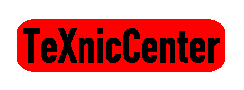
\includegraphics{txc.eps}
	\end{center}
	\caption{A Figure to stress the StructureParser}
\end{figure}

\begin{figure}
	\begin{center}
		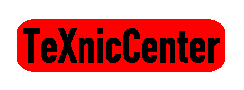
\includegraphics{txc.eps}
	\end{center}
	\caption{A Figure to stress the StructureParser}
\end{figure}

\begin{figure}
	\begin{center}
		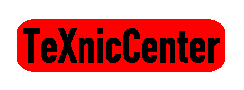
\includegraphics{txc.eps}
	\end{center}
	\caption{A Figure to stress the StructureParser}
\end{figure}

\begin{figure}
	\begin{center}
		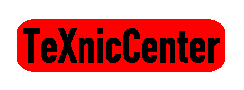
\includegraphics{txc.eps}
	\end{center}
	\caption{A Figure to stress the StructureParser}
\end{figure}

\begin{figure}
	\begin{center}
		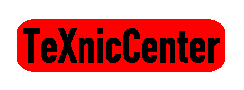
\includegraphics{txc.eps}
	\end{center}
	\caption{A Figure to stress the StructureParser}
\end{figure}


\clearpage


\begin{figure}
	\begin{center}
		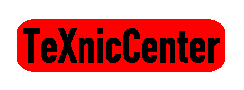
\includegraphics{txc.eps}
	\end{center}
	\caption{A Figure to stress the StructureParser}
\end{figure}

\begin{figure}
	\begin{center}
		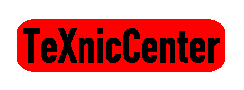
\includegraphics{txc.eps}
	\end{center}
	\caption{A Figure to stress the StructureParser}
\end{figure}

\begin{figure}
	\begin{center}
		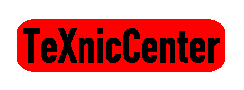
\includegraphics{txc.eps}
	\end{center}
	\caption{A Figure to stress the StructureParser}
\end{figure}

\begin{figure}
	\begin{center}
		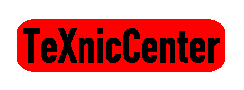
\includegraphics{txc.eps}
	\end{center}
	\caption{A Figure to stress the StructureParser}
\end{figure}

\begin{figure}
	\begin{center}
		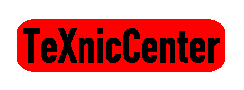
\includegraphics{txc.eps}
	\end{center}
	\caption{A Figure to stress the StructureParser}
\end{figure}


\clearpage


\begin{figure}
	\begin{center}
		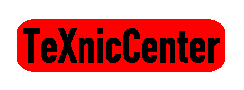
\includegraphics{txc.eps}
	\end{center}
	\caption{A Figure to stress the StructureParser}
\end{figure}

\begin{figure}
	\begin{center}
		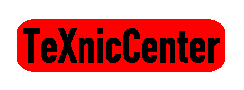
\includegraphics{txc.eps}
	\end{center}
	\caption{A Figure to stress the StructureParser}
\end{figure}

\begin{figure}
	\begin{center}
		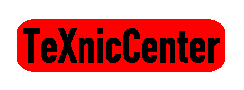
\includegraphics{txc.eps}
	\end{center}
	\caption{A Figure to stress the StructureParser}
\end{figure}

\begin{figure}
	\begin{center}
		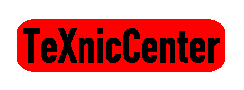
\includegraphics{txc.eps}
	\end{center}
	\caption{A Figure to stress the StructureParser}
\end{figure}

\begin{figure}
	\begin{center}
		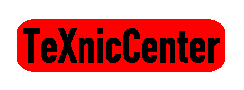
\includegraphics{txc.eps}
	\end{center}
	\caption{A Figure to stress the StructureParser}
\end{figure}


\clearpage


\begin{figure}
	\begin{center}
		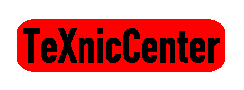
\includegraphics{txc.eps}
	\end{center}
	\caption{A Figure to stress the StructureParser}
\end{figure}

\begin{figure}
	\begin{center}
		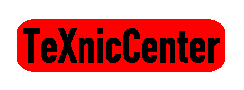
\includegraphics{txc.eps}
	\end{center}
	\caption{A Figure to stress the StructureParser}
\end{figure}

\begin{figure}
	\begin{center}
		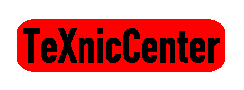
\includegraphics{txc.eps}
	\end{center}
	\caption{A Figure to stress the StructureParser}
\end{figure}

\begin{figure}
	\begin{center}
		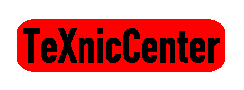
\includegraphics{txc.eps}
	\end{center}
	\caption{A Figure to stress the StructureParser}
\end{figure}

\begin{figure}
	\begin{center}
		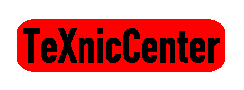
\includegraphics{txc.eps}
	\end{center}
	\caption{A Figure to stress the StructureParser}
\end{figure}


\clearpage

\begin{figure}
	\begin{center}
		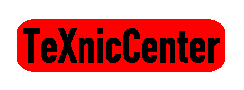
\includegraphics{txc.eps}
	\end{center}
	\caption{A Figure to stress the StructureParser}
\end{figure}

\begin{figure}
	\begin{center}
		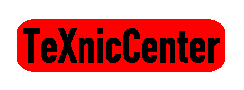
\includegraphics{txc.eps}
	\end{center}
	\caption{A Figure to stress the StructureParser}
\end{figure}

\begin{figure}
	\begin{center}
		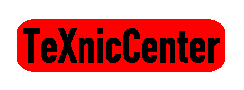
\includegraphics{txc.eps}
	\end{center}
	\caption{A Figure to stress the StructureParser}
\end{figure}

\begin{figure}
	\begin{center}
		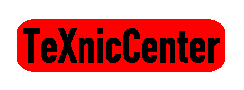
\includegraphics{txc.eps}
	\end{center}
	\caption{A Figure to stress the StructureParser}
\end{figure}

\begin{figure}
	\begin{center}
		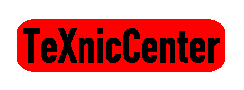
\includegraphics{txc.eps}
	\end{center}
	\caption{A Figure to stress the StructureParser}
\end{figure}


\clearpage


%%%%%%%%%%%%%%%%%%%%%%%%%%%%%%%%%%%%%%%%%%%%%%%%%%%%%%%%%%%%%%%%%%%%%%%%
%% $Id$
%%%%%%%%%%%%%%%%%%%%%%%%%%%%%%%%%%%%%%%%%%%%%%%%%%%%%%%%%%%%%%%%%%%%%%%%
% This file and the files in this directory and its subdirectories
% are intended to test several parts of the TeXnicCenter-system.
%
% Copyright (C) 2002-$CurrentYear$ ToolsCenter

% Their main purpose is to reproduce several bugs or behaviours coming
% up from missing features. They are neither a good starting point for
% working with TeX nor with the TeXnicCenter-system. If you use them,
% you do this on your own risk. They come WITHOUT ANY WARRANTY;
% without even the implied warranty of MERCHANTABILITY or
% FITNESS FOR A PARTICULAR PURPOSE.
%
% Anything below the "end of prolog"-line is for testing purposes only
% and does not reflect the opinions of the author(s) and is not meant
% to be a statement at all; it is even not said to be true or reliable.
%
% If you have further questions or if you want to support
% further TeXnicCenter development, visit the TeXnicCenter-homepage
%
%     http://www.ToolsCenter.org
%
% end of prolog %%%%%%%%%%%%%%%%%%%%%%%%%%%%%%%%%%%%%%%%%%%%%%%%%%%%%%%%

% 25 Graphics

\begin{figure}
	\begin{center}
		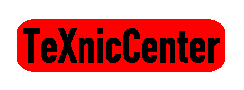
\includegraphics{txc.eps}
	\end{center}
	\caption{A Figure to stress the StructureParser}
\end{figure}

\begin{figure}
	\begin{center}
		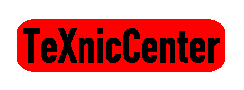
\includegraphics{txc.eps}
	\end{center}
	\caption{A Figure to stress the StructureParser}
\end{figure}

\begin{figure}
	\begin{center}
		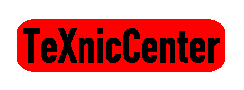
\includegraphics{txc.eps}
	\end{center}
	\caption{A Figure to stress the StructureParser}
\end{figure}

\begin{figure}
	\begin{center}
		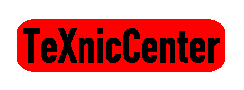
\includegraphics{txc.eps}
	\end{center}
	\caption{A Figure to stress the StructureParser}
\end{figure}

\begin{figure}
	\begin{center}
		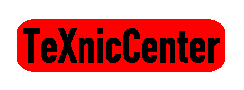
\includegraphics{txc.eps}
	\end{center}
	\caption{A Figure to stress the StructureParser}
\end{figure}


\clearpage


\begin{figure}
	\begin{center}
		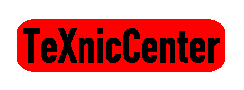
\includegraphics{txc.eps}
	\end{center}
	\caption{A Figure to stress the StructureParser}
\end{figure}

\begin{figure}
	\begin{center}
		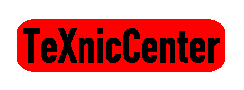
\includegraphics{txc.eps}
	\end{center}
	\caption{A Figure to stress the StructureParser}
\end{figure}

\begin{figure}
	\begin{center}
		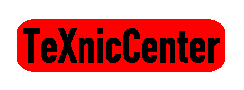
\includegraphics{txc.eps}
	\end{center}
	\caption{A Figure to stress the StructureParser}
\end{figure}

\begin{figure}
	\begin{center}
		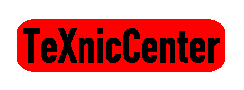
\includegraphics{txc.eps}
	\end{center}
	\caption{A Figure to stress the StructureParser}
\end{figure}

\begin{figure}
	\begin{center}
		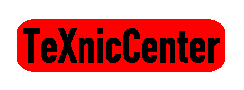
\includegraphics{txc.eps}
	\end{center}
	\caption{A Figure to stress the StructureParser}
\end{figure}


\clearpage


\begin{figure}
	\begin{center}
		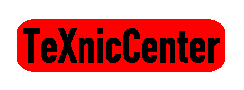
\includegraphics{txc.eps}
	\end{center}
	\caption{A Figure to stress the StructureParser}
\end{figure}

\begin{figure}
	\begin{center}
		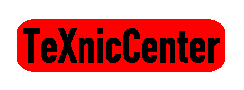
\includegraphics{txc.eps}
	\end{center}
	\caption{A Figure to stress the StructureParser}
\end{figure}

\begin{figure}
	\begin{center}
		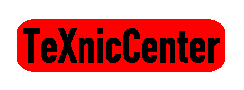
\includegraphics{txc.eps}
	\end{center}
	\caption{A Figure to stress the StructureParser}
\end{figure}

\begin{figure}
	\begin{center}
		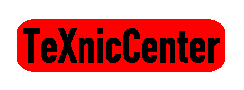
\includegraphics{txc.eps}
	\end{center}
	\caption{A Figure to stress the StructureParser}
\end{figure}

\begin{figure}
	\begin{center}
		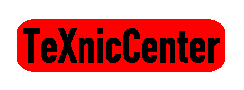
\includegraphics{txc.eps}
	\end{center}
	\caption{A Figure to stress the StructureParser}
\end{figure}


\clearpage


\begin{figure}
	\begin{center}
		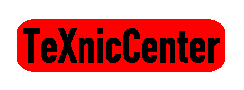
\includegraphics{txc.eps}
	\end{center}
	\caption{A Figure to stress the StructureParser}
\end{figure}

\begin{figure}
	\begin{center}
		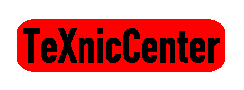
\includegraphics{txc.eps}
	\end{center}
	\caption{A Figure to stress the StructureParser}
\end{figure}

\begin{figure}
	\begin{center}
		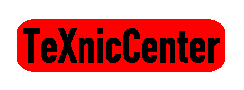
\includegraphics{txc.eps}
	\end{center}
	\caption{A Figure to stress the StructureParser}
\end{figure}

\begin{figure}
	\begin{center}
		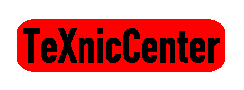
\includegraphics{txc.eps}
	\end{center}
	\caption{A Figure to stress the StructureParser}
\end{figure}

\begin{figure}
	\begin{center}
		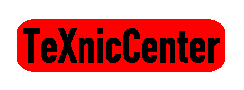
\includegraphics{txc.eps}
	\end{center}
	\caption{A Figure to stress the StructureParser}
\end{figure}


\clearpage

\begin{figure}
	\begin{center}
		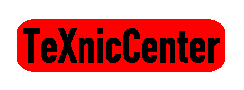
\includegraphics{txc.eps}
	\end{center}
	\caption{A Figure to stress the StructureParser}
\end{figure}

\begin{figure}
	\begin{center}
		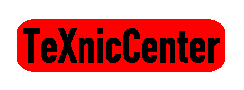
\includegraphics{txc.eps}
	\end{center}
	\caption{A Figure to stress the StructureParser}
\end{figure}

\begin{figure}
	\begin{center}
		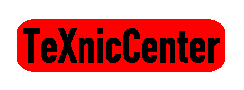
\includegraphics{txc.eps}
	\end{center}
	\caption{A Figure to stress the StructureParser}
\end{figure}

\begin{figure}
	\begin{center}
		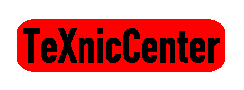
\includegraphics{txc.eps}
	\end{center}
	\caption{A Figure to stress the StructureParser}
\end{figure}

\begin{figure}
	\begin{center}
		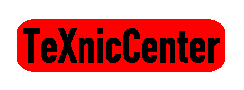
\includegraphics{txc.eps}
	\end{center}
	\caption{A Figure to stress the StructureParser}
\end{figure}


\clearpage


%%%%%%%%%%%%%%%%%%%%%%%%%%%%%%%%%%%%%%%%%%%%%%%%%%%%%%%%%%%%%%%%%%%%%%%%
%% $Id$
%%%%%%%%%%%%%%%%%%%%%%%%%%%%%%%%%%%%%%%%%%%%%%%%%%%%%%%%%%%%%%%%%%%%%%%%
% This file and the files in this directory and its subdirectories
% are intended to test several parts of the TeXnicCenter-system.
%
% Copyright (C) 2002-$CurrentYear$ ToolsCenter

% Their main purpose is to reproduce several bugs or behaviours coming
% up from missing features. They are neither a good starting point for
% working with TeX nor with the TeXnicCenter-system. If you use them,
% you do this on your own risk. They come WITHOUT ANY WARRANTY;
% without even the implied warranty of MERCHANTABILITY or
% FITNESS FOR A PARTICULAR PURPOSE.
%
% Anything below the "end of prolog"-line is for testing purposes only
% and does not reflect the opinions of the author(s) and is not meant
% to be a statement at all; it is even not said to be true or reliable.
%
% If you have further questions or if you want to support
% further TeXnicCenter development, visit the TeXnicCenter-homepage
%
%     http://www.ToolsCenter.org
%
% end of prolog %%%%%%%%%%%%%%%%%%%%%%%%%%%%%%%%%%%%%%%%%%%%%%%%%%%%%%%%

% 25 Graphics

\begin{figure}
	\begin{center}
		\includegraphics{txc.eps}
	\end{center}
	\caption{A Figure to stress the StructureParser}
\end{figure}

\begin{figure}
	\begin{center}
		\includegraphics{txc.eps}
	\end{center}
	\caption{A Figure to stress the StructureParser}
\end{figure}

\begin{figure}
	\begin{center}
		\includegraphics{txc.eps}
	\end{center}
	\caption{A Figure to stress the StructureParser}
\end{figure}

\begin{figure}
	\begin{center}
		\includegraphics{txc.eps}
	\end{center}
	\caption{A Figure to stress the StructureParser}
\end{figure}

\begin{figure}
	\begin{center}
		\includegraphics{txc.eps}
	\end{center}
	\caption{A Figure to stress the StructureParser}
\end{figure}


\clearpage


\begin{figure}
	\begin{center}
		\includegraphics{txc.eps}
	\end{center}
	\caption{A Figure to stress the StructureParser}
\end{figure}

\begin{figure}
	\begin{center}
		\includegraphics{txc.eps}
	\end{center}
	\caption{A Figure to stress the StructureParser}
\end{figure}

\begin{figure}
	\begin{center}
		\includegraphics{txc.eps}
	\end{center}
	\caption{A Figure to stress the StructureParser}
\end{figure}

\begin{figure}
	\begin{center}
		\includegraphics{txc.eps}
	\end{center}
	\caption{A Figure to stress the StructureParser}
\end{figure}

\begin{figure}
	\begin{center}
		\includegraphics{txc.eps}
	\end{center}
	\caption{A Figure to stress the StructureParser}
\end{figure}


\clearpage


\begin{figure}
	\begin{center}
		\includegraphics{txc.eps}
	\end{center}
	\caption{A Figure to stress the StructureParser}
\end{figure}

\begin{figure}
	\begin{center}
		\includegraphics{txc.eps}
	\end{center}
	\caption{A Figure to stress the StructureParser}
\end{figure}

\begin{figure}
	\begin{center}
		\includegraphics{txc.eps}
	\end{center}
	\caption{A Figure to stress the StructureParser}
\end{figure}

\begin{figure}
	\begin{center}
		\includegraphics{txc.eps}
	\end{center}
	\caption{A Figure to stress the StructureParser}
\end{figure}

\begin{figure}
	\begin{center}
		\includegraphics{txc.eps}
	\end{center}
	\caption{A Figure to stress the StructureParser}
\end{figure}


\clearpage


\begin{figure}
	\begin{center}
		\includegraphics{txc.eps}
	\end{center}
	\caption{A Figure to stress the StructureParser}
\end{figure}

\begin{figure}
	\begin{center}
		\includegraphics{txc.eps}
	\end{center}
	\caption{A Figure to stress the StructureParser}
\end{figure}

\begin{figure}
	\begin{center}
		\includegraphics{txc.eps}
	\end{center}
	\caption{A Figure to stress the StructureParser}
\end{figure}

\begin{figure}
	\begin{center}
		\includegraphics{txc.eps}
	\end{center}
	\caption{A Figure to stress the StructureParser}
\end{figure}

\begin{figure}
	\begin{center}
		\includegraphics{txc.eps}
	\end{center}
	\caption{A Figure to stress the StructureParser}
\end{figure}


\clearpage

\begin{figure}
	\begin{center}
		\includegraphics{txc.eps}
	\end{center}
	\caption{A Figure to stress the StructureParser}
\end{figure}

\begin{figure}
	\begin{center}
		\includegraphics{txc.eps}
	\end{center}
	\caption{A Figure to stress the StructureParser}
\end{figure}

\begin{figure}
	\begin{center}
		\includegraphics{txc.eps}
	\end{center}
	\caption{A Figure to stress the StructureParser}
\end{figure}

\begin{figure}
	\begin{center}
		\includegraphics{txc.eps}
	\end{center}
	\caption{A Figure to stress the StructureParser}
\end{figure}

\begin{figure}
	\begin{center}
		\includegraphics{txc.eps}
	\end{center}
	\caption{A Figure to stress the StructureParser}
\end{figure}


\clearpage


%%%%%%%%%%%%%%%%%%%%%%%%%%%%%%%%%%%%%%%%%%%%%%%%%%%%%%%%%%%%%%%%%%%%%%%%
%% $Id$
%%%%%%%%%%%%%%%%%%%%%%%%%%%%%%%%%%%%%%%%%%%%%%%%%%%%%%%%%%%%%%%%%%%%%%%%
% This file and the files in this directory and its subdirectories
% are intended to test several parts of the TeXnicCenter-system.
%
% Copyright (C) 2002-$CurrentYear$ ToolsCenter

% Their main purpose is to reproduce several bugs or behaviours coming
% up from missing features. They are neither a good starting point for
% working with TeX nor with the TeXnicCenter-system. If you use them,
% you do this on your own risk. They come WITHOUT ANY WARRANTY;
% without even the implied warranty of MERCHANTABILITY or
% FITNESS FOR A PARTICULAR PURPOSE.
%
% Anything below the "end of prolog"-line is for testing purposes only
% and does not reflect the opinions of the author(s) and is not meant
% to be a statement at all; it is even not said to be true or reliable.
%
% If you have further questions or if you want to support
% further TeXnicCenter development, visit the TeXnicCenter-homepage
%
%     http://www.ToolsCenter.org
%
% end of prolog %%%%%%%%%%%%%%%%%%%%%%%%%%%%%%%%%%%%%%%%%%%%%%%%%%%%%%%%

% 25 Graphics

\begin{figure}
	\begin{center}
		\includegraphics{txc.eps}
	\end{center}
	\caption{A Figure to stress the StructureParser}
\end{figure}

\begin{figure}
	\begin{center}
		\includegraphics{txc.eps}
	\end{center}
	\caption{A Figure to stress the StructureParser}
\end{figure}

\begin{figure}
	\begin{center}
		\includegraphics{txc.eps}
	\end{center}
	\caption{A Figure to stress the StructureParser}
\end{figure}

\begin{figure}
	\begin{center}
		\includegraphics{txc.eps}
	\end{center}
	\caption{A Figure to stress the StructureParser}
\end{figure}

\begin{figure}
	\begin{center}
		\includegraphics{txc.eps}
	\end{center}
	\caption{A Figure to stress the StructureParser}
\end{figure}


\clearpage


\begin{figure}
	\begin{center}
		\includegraphics{txc.eps}
	\end{center}
	\caption{A Figure to stress the StructureParser}
\end{figure}

\begin{figure}
	\begin{center}
		\includegraphics{txc.eps}
	\end{center}
	\caption{A Figure to stress the StructureParser}
\end{figure}

\begin{figure}
	\begin{center}
		\includegraphics{txc.eps}
	\end{center}
	\caption{A Figure to stress the StructureParser}
\end{figure}

\begin{figure}
	\begin{center}
		\includegraphics{txc.eps}
	\end{center}
	\caption{A Figure to stress the StructureParser}
\end{figure}

\begin{figure}
	\begin{center}
		\includegraphics{txc.eps}
	\end{center}
	\caption{A Figure to stress the StructureParser}
\end{figure}


\clearpage


\begin{figure}
	\begin{center}
		\includegraphics{txc.eps}
	\end{center}
	\caption{A Figure to stress the StructureParser}
\end{figure}

\begin{figure}
	\begin{center}
		\includegraphics{txc.eps}
	\end{center}
	\caption{A Figure to stress the StructureParser}
\end{figure}

\begin{figure}
	\begin{center}
		\includegraphics{txc.eps}
	\end{center}
	\caption{A Figure to stress the StructureParser}
\end{figure}

\begin{figure}
	\begin{center}
		\includegraphics{txc.eps}
	\end{center}
	\caption{A Figure to stress the StructureParser}
\end{figure}

\begin{figure}
	\begin{center}
		\includegraphics{txc.eps}
	\end{center}
	\caption{A Figure to stress the StructureParser}
\end{figure}


\clearpage


\begin{figure}
	\begin{center}
		\includegraphics{txc.eps}
	\end{center}
	\caption{A Figure to stress the StructureParser}
\end{figure}

\begin{figure}
	\begin{center}
		\includegraphics{txc.eps}
	\end{center}
	\caption{A Figure to stress the StructureParser}
\end{figure}

\begin{figure}
	\begin{center}
		\includegraphics{txc.eps}
	\end{center}
	\caption{A Figure to stress the StructureParser}
\end{figure}

\begin{figure}
	\begin{center}
		\includegraphics{txc.eps}
	\end{center}
	\caption{A Figure to stress the StructureParser}
\end{figure}

\begin{figure}
	\begin{center}
		\includegraphics{txc.eps}
	\end{center}
	\caption{A Figure to stress the StructureParser}
\end{figure}


\clearpage

\begin{figure}
	\begin{center}
		\includegraphics{txc.eps}
	\end{center}
	\caption{A Figure to stress the StructureParser}
\end{figure}

\begin{figure}
	\begin{center}
		\includegraphics{txc.eps}
	\end{center}
	\caption{A Figure to stress the StructureParser}
\end{figure}

\begin{figure}
	\begin{center}
		\includegraphics{txc.eps}
	\end{center}
	\caption{A Figure to stress the StructureParser}
\end{figure}

\begin{figure}
	\begin{center}
		\includegraphics{txc.eps}
	\end{center}
	\caption{A Figure to stress the StructureParser}
\end{figure}

\begin{figure}
	\begin{center}
		\includegraphics{txc.eps}
	\end{center}
	\caption{A Figure to stress the StructureParser}
\end{figure}


\clearpage


%%%%%%%%%%%%%%%%%%%%%%%%%%%%%%%%%%%%%%%%%%%%%%%%%%%%%%%%%%%%%%%%%%%%%%%%
%% $Id$
%%%%%%%%%%%%%%%%%%%%%%%%%%%%%%%%%%%%%%%%%%%%%%%%%%%%%%%%%%%%%%%%%%%%%%%%
% This file and the files in this directory and its subdirectories
% are intended to test several parts of the TeXnicCenter-system.
%
% Copyright (C) 2002-$CurrentYear$ ToolsCenter

% Their main purpose is to reproduce several bugs or behaviours coming
% up from missing features. They are neither a good starting point for
% working with TeX nor with the TeXnicCenter-system. If you use them,
% you do this on your own risk. They come WITHOUT ANY WARRANTY;
% without even the implied warranty of MERCHANTABILITY or
% FITNESS FOR A PARTICULAR PURPOSE.
%
% Anything below the "end of prolog"-line is for testing purposes only
% and does not reflect the opinions of the author(s) and is not meant
% to be a statement at all; it is even not said to be true or reliable.
%
% If you have further questions or if you want to support
% further TeXnicCenter development, visit the TeXnicCenter-homepage
%
%     http://www.ToolsCenter.org
%
% end of prolog %%%%%%%%%%%%%%%%%%%%%%%%%%%%%%%%%%%%%%%%%%%%%%%%%%%%%%%%

% 25 Graphics

\begin{figure}
	\begin{center}
		\includegraphics{txc.eps}
	\end{center}
	\caption{A Figure to stress the StructureParser}
\end{figure}

\begin{figure}
	\begin{center}
		\includegraphics{txc.eps}
	\end{center}
	\caption{A Figure to stress the StructureParser}
\end{figure}

\begin{figure}
	\begin{center}
		\includegraphics{txc.eps}
	\end{center}
	\caption{A Figure to stress the StructureParser}
\end{figure}

\begin{figure}
	\begin{center}
		\includegraphics{txc.eps}
	\end{center}
	\caption{A Figure to stress the StructureParser}
\end{figure}

\begin{figure}
	\begin{center}
		\includegraphics{txc.eps}
	\end{center}
	\caption{A Figure to stress the StructureParser}
\end{figure}


\clearpage


\begin{figure}
	\begin{center}
		\includegraphics{txc.eps}
	\end{center}
	\caption{A Figure to stress the StructureParser}
\end{figure}

\begin{figure}
	\begin{center}
		\includegraphics{txc.eps}
	\end{center}
	\caption{A Figure to stress the StructureParser}
\end{figure}

\begin{figure}
	\begin{center}
		\includegraphics{txc.eps}
	\end{center}
	\caption{A Figure to stress the StructureParser}
\end{figure}

\begin{figure}
	\begin{center}
		\includegraphics{txc.eps}
	\end{center}
	\caption{A Figure to stress the StructureParser}
\end{figure}

\begin{figure}
	\begin{center}
		\includegraphics{txc.eps}
	\end{center}
	\caption{A Figure to stress the StructureParser}
\end{figure}


\clearpage


\begin{figure}
	\begin{center}
		\includegraphics{txc.eps}
	\end{center}
	\caption{A Figure to stress the StructureParser}
\end{figure}

\begin{figure}
	\begin{center}
		\includegraphics{txc.eps}
	\end{center}
	\caption{A Figure to stress the StructureParser}
\end{figure}

\begin{figure}
	\begin{center}
		\includegraphics{txc.eps}
	\end{center}
	\caption{A Figure to stress the StructureParser}
\end{figure}

\begin{figure}
	\begin{center}
		\includegraphics{txc.eps}
	\end{center}
	\caption{A Figure to stress the StructureParser}
\end{figure}

\begin{figure}
	\begin{center}
		\includegraphics{txc.eps}
	\end{center}
	\caption{A Figure to stress the StructureParser}
\end{figure}


\clearpage


\begin{figure}
	\begin{center}
		\includegraphics{txc.eps}
	\end{center}
	\caption{A Figure to stress the StructureParser}
\end{figure}

\begin{figure}
	\begin{center}
		\includegraphics{txc.eps}
	\end{center}
	\caption{A Figure to stress the StructureParser}
\end{figure}

\begin{figure}
	\begin{center}
		\includegraphics{txc.eps}
	\end{center}
	\caption{A Figure to stress the StructureParser}
\end{figure}

\begin{figure}
	\begin{center}
		\includegraphics{txc.eps}
	\end{center}
	\caption{A Figure to stress the StructureParser}
\end{figure}

\begin{figure}
	\begin{center}
		\includegraphics{txc.eps}
	\end{center}
	\caption{A Figure to stress the StructureParser}
\end{figure}


\clearpage

\begin{figure}
	\begin{center}
		\includegraphics{txc.eps}
	\end{center}
	\caption{A Figure to stress the StructureParser}
\end{figure}

\begin{figure}
	\begin{center}
		\includegraphics{txc.eps}
	\end{center}
	\caption{A Figure to stress the StructureParser}
\end{figure}

\begin{figure}
	\begin{center}
		\includegraphics{txc.eps}
	\end{center}
	\caption{A Figure to stress the StructureParser}
\end{figure}

\begin{figure}
	\begin{center}
		\includegraphics{txc.eps}
	\end{center}
	\caption{A Figure to stress the StructureParser}
\end{figure}

\begin{figure}
	\begin{center}
		\includegraphics{txc.eps}
	\end{center}
	\caption{A Figure to stress the StructureParser}
\end{figure}


\clearpage


%%%%%%%%%%%%%%%%%%%%%%%%%%%%%%%%%%%%%%%%%%%%%%%%%%%%%%%%%%%%%%%%%%%%%%%%
%% $Id$
%%%%%%%%%%%%%%%%%%%%%%%%%%%%%%%%%%%%%%%%%%%%%%%%%%%%%%%%%%%%%%%%%%%%%%%%
% This file and the files in this directory and its subdirectories
% are intended to test several parts of the TeXnicCenter-system.
%
% Copyright (C) 2002-$CurrentYear$ ToolsCenter

% Their main purpose is to reproduce several bugs or behaviours coming
% up from missing features. They are neither a good starting point for
% working with TeX nor with the TeXnicCenter-system. If you use them,
% you do this on your own risk. They come WITHOUT ANY WARRANTY;
% without even the implied warranty of MERCHANTABILITY or
% FITNESS FOR A PARTICULAR PURPOSE.
%
% Anything below the "end of prolog"-line is for testing purposes only
% and does not reflect the opinions of the author(s) and is not meant
% to be a statement at all; it is even not said to be true or reliable.
%
% If you have further questions or if you want to support
% further TeXnicCenter development, visit the TeXnicCenter-homepage
%
%     http://www.ToolsCenter.org
%
% end of prolog %%%%%%%%%%%%%%%%%%%%%%%%%%%%%%%%%%%%%%%%%%%%%%%%%%%%%%%%

% 25 Graphics

\begin{figure}
	\begin{center}
		\includegraphics{txc.eps}
	\end{center}
	\caption{A Figure to stress the StructureParser}
\end{figure}

\begin{figure}
	\begin{center}
		\includegraphics{txc.eps}
	\end{center}
	\caption{A Figure to stress the StructureParser}
\end{figure}

\begin{figure}
	\begin{center}
		\includegraphics{txc.eps}
	\end{center}
	\caption{A Figure to stress the StructureParser}
\end{figure}

\begin{figure}
	\begin{center}
		\includegraphics{txc.eps}
	\end{center}
	\caption{A Figure to stress the StructureParser}
\end{figure}

\begin{figure}
	\begin{center}
		\includegraphics{txc.eps}
	\end{center}
	\caption{A Figure to stress the StructureParser}
\end{figure}


\clearpage


\begin{figure}
	\begin{center}
		\includegraphics{txc.eps}
	\end{center}
	\caption{A Figure to stress the StructureParser}
\end{figure}

\begin{figure}
	\begin{center}
		\includegraphics{txc.eps}
	\end{center}
	\caption{A Figure to stress the StructureParser}
\end{figure}

\begin{figure}
	\begin{center}
		\includegraphics{txc.eps}
	\end{center}
	\caption{A Figure to stress the StructureParser}
\end{figure}

\begin{figure}
	\begin{center}
		\includegraphics{txc.eps}
	\end{center}
	\caption{A Figure to stress the StructureParser}
\end{figure}

\begin{figure}
	\begin{center}
		\includegraphics{txc.eps}
	\end{center}
	\caption{A Figure to stress the StructureParser}
\end{figure}


\clearpage


\begin{figure}
	\begin{center}
		\includegraphics{txc.eps}
	\end{center}
	\caption{A Figure to stress the StructureParser}
\end{figure}

\begin{figure}
	\begin{center}
		\includegraphics{txc.eps}
	\end{center}
	\caption{A Figure to stress the StructureParser}
\end{figure}

\begin{figure}
	\begin{center}
		\includegraphics{txc.eps}
	\end{center}
	\caption{A Figure to stress the StructureParser}
\end{figure}

\begin{figure}
	\begin{center}
		\includegraphics{txc.eps}
	\end{center}
	\caption{A Figure to stress the StructureParser}
\end{figure}

\begin{figure}
	\begin{center}
		\includegraphics{txc.eps}
	\end{center}
	\caption{A Figure to stress the StructureParser}
\end{figure}


\clearpage


\begin{figure}
	\begin{center}
		\includegraphics{txc.eps}
	\end{center}
	\caption{A Figure to stress the StructureParser}
\end{figure}

\begin{figure}
	\begin{center}
		\includegraphics{txc.eps}
	\end{center}
	\caption{A Figure to stress the StructureParser}
\end{figure}

\begin{figure}
	\begin{center}
		\includegraphics{txc.eps}
	\end{center}
	\caption{A Figure to stress the StructureParser}
\end{figure}

\begin{figure}
	\begin{center}
		\includegraphics{txc.eps}
	\end{center}
	\caption{A Figure to stress the StructureParser}
\end{figure}

\begin{figure}
	\begin{center}
		\includegraphics{txc.eps}
	\end{center}
	\caption{A Figure to stress the StructureParser}
\end{figure}


\clearpage

\begin{figure}
	\begin{center}
		\includegraphics{txc.eps}
	\end{center}
	\caption{A Figure to stress the StructureParser}
\end{figure}

\begin{figure}
	\begin{center}
		\includegraphics{txc.eps}
	\end{center}
	\caption{A Figure to stress the StructureParser}
\end{figure}

\begin{figure}
	\begin{center}
		\includegraphics{txc.eps}
	\end{center}
	\caption{A Figure to stress the StructureParser}
\end{figure}

\begin{figure}
	\begin{center}
		\includegraphics{txc.eps}
	\end{center}
	\caption{A Figure to stress the StructureParser}
\end{figure}

\begin{figure}
	\begin{center}
		\includegraphics{txc.eps}
	\end{center}
	\caption{A Figure to stress the StructureParser}
\end{figure}


\clearpage


%%%%%%%%%%%%%%%%%%%%%%%%%%%%%%%%%%%%%%%%%%%%%%%%%%%%%%%%%%%%%%%%%%%%%%%%
%% $Id$
%%%%%%%%%%%%%%%%%%%%%%%%%%%%%%%%%%%%%%%%%%%%%%%%%%%%%%%%%%%%%%%%%%%%%%%%
% This file and the files in this directory and its subdirectories
% are intended to test several parts of the TeXnicCenter-system.
%
% Copyright (C) 2002-$CurrentYear$ ToolsCenter

% Their main purpose is to reproduce several bugs or behaviours coming
% up from missing features. They are neither a good starting point for
% working with TeX nor with the TeXnicCenter-system. If you use them,
% you do this on your own risk. They come WITHOUT ANY WARRANTY;
% without even the implied warranty of MERCHANTABILITY or
% FITNESS FOR A PARTICULAR PURPOSE.
%
% Anything below the "end of prolog"-line is for testing purposes only
% and does not reflect the opinions of the author(s) and is not meant
% to be a statement at all; it is even not said to be true or reliable.
%
% If you have further questions or if you want to support
% further TeXnicCenter development, visit the TeXnicCenter-homepage
%
%     http://www.ToolsCenter.org
%
% end of prolog %%%%%%%%%%%%%%%%%%%%%%%%%%%%%%%%%%%%%%%%%%%%%%%%%%%%%%%%

% 25 Graphics

\begin{figure}
	\begin{center}
		\includegraphics{txc.eps}
	\end{center}
	\caption{A Figure to stress the StructureParser}
\end{figure}

\begin{figure}
	\begin{center}
		\includegraphics{txc.eps}
	\end{center}
	\caption{A Figure to stress the StructureParser}
\end{figure}

\begin{figure}
	\begin{center}
		\includegraphics{txc.eps}
	\end{center}
	\caption{A Figure to stress the StructureParser}
\end{figure}

\begin{figure}
	\begin{center}
		\includegraphics{txc.eps}
	\end{center}
	\caption{A Figure to stress the StructureParser}
\end{figure}

\begin{figure}
	\begin{center}
		\includegraphics{txc.eps}
	\end{center}
	\caption{A Figure to stress the StructureParser}
\end{figure}


\clearpage


\begin{figure}
	\begin{center}
		\includegraphics{txc.eps}
	\end{center}
	\caption{A Figure to stress the StructureParser}
\end{figure}

\begin{figure}
	\begin{center}
		\includegraphics{txc.eps}
	\end{center}
	\caption{A Figure to stress the StructureParser}
\end{figure}

\begin{figure}
	\begin{center}
		\includegraphics{txc.eps}
	\end{center}
	\caption{A Figure to stress the StructureParser}
\end{figure}

\begin{figure}
	\begin{center}
		\includegraphics{txc.eps}
	\end{center}
	\caption{A Figure to stress the StructureParser}
\end{figure}

\begin{figure}
	\begin{center}
		\includegraphics{txc.eps}
	\end{center}
	\caption{A Figure to stress the StructureParser}
\end{figure}


\clearpage


\begin{figure}
	\begin{center}
		\includegraphics{txc.eps}
	\end{center}
	\caption{A Figure to stress the StructureParser}
\end{figure}

\begin{figure}
	\begin{center}
		\includegraphics{txc.eps}
	\end{center}
	\caption{A Figure to stress the StructureParser}
\end{figure}

\begin{figure}
	\begin{center}
		\includegraphics{txc.eps}
	\end{center}
	\caption{A Figure to stress the StructureParser}
\end{figure}

\begin{figure}
	\begin{center}
		\includegraphics{txc.eps}
	\end{center}
	\caption{A Figure to stress the StructureParser}
\end{figure}

\begin{figure}
	\begin{center}
		\includegraphics{txc.eps}
	\end{center}
	\caption{A Figure to stress the StructureParser}
\end{figure}


\clearpage


\begin{figure}
	\begin{center}
		\includegraphics{txc.eps}
	\end{center}
	\caption{A Figure to stress the StructureParser}
\end{figure}

\begin{figure}
	\begin{center}
		\includegraphics{txc.eps}
	\end{center}
	\caption{A Figure to stress the StructureParser}
\end{figure}

\begin{figure}
	\begin{center}
		\includegraphics{txc.eps}
	\end{center}
	\caption{A Figure to stress the StructureParser}
\end{figure}

\begin{figure}
	\begin{center}
		\includegraphics{txc.eps}
	\end{center}
	\caption{A Figure to stress the StructureParser}
\end{figure}

\begin{figure}
	\begin{center}
		\includegraphics{txc.eps}
	\end{center}
	\caption{A Figure to stress the StructureParser}
\end{figure}


\clearpage

\begin{figure}
	\begin{center}
		\includegraphics{txc.eps}
	\end{center}
	\caption{A Figure to stress the StructureParser}
\end{figure}

\begin{figure}
	\begin{center}
		\includegraphics{txc.eps}
	\end{center}
	\caption{A Figure to stress the StructureParser}
\end{figure}

\begin{figure}
	\begin{center}
		\includegraphics{txc.eps}
	\end{center}
	\caption{A Figure to stress the StructureParser}
\end{figure}

\begin{figure}
	\begin{center}
		\includegraphics{txc.eps}
	\end{center}
	\caption{A Figure to stress the StructureParser}
\end{figure}

\begin{figure}
	\begin{center}
		\includegraphics{txc.eps}
	\end{center}
	\caption{A Figure to stress the StructureParser}
\end{figure}


\clearpage


%%%%%%%%%%%%%%%%%%%%%%%%%%%%%%%%%%%%%%%%%%%%%%%%%%%%%%%%%%%%%%%%%%%%%%%%
%% $Id$
%%%%%%%%%%%%%%%%%%%%%%%%%%%%%%%%%%%%%%%%%%%%%%%%%%%%%%%%%%%%%%%%%%%%%%%%
% This file and the files in this directory and its subdirectories
% are intended to test several parts of the TeXnicCenter-system.
%
% Copyright (C) 2002-$CurrentYear$ ToolsCenter

% Their main purpose is to reproduce several bugs or behaviours coming
% up from missing features. They are neither a good starting point for
% working with TeX nor with the TeXnicCenter-system. If you use them,
% you do this on your own risk. They come WITHOUT ANY WARRANTY;
% without even the implied warranty of MERCHANTABILITY or
% FITNESS FOR A PARTICULAR PURPOSE.
%
% Anything below the "end of prolog"-line is for testing purposes only
% and does not reflect the opinions of the author(s) and is not meant
% to be a statement at all; it is even not said to be true or reliable.
%
% If you have further questions or if you want to support
% further TeXnicCenter development, visit the TeXnicCenter-homepage
%
%     http://www.ToolsCenter.org
%
% end of prolog %%%%%%%%%%%%%%%%%%%%%%%%%%%%%%%%%%%%%%%%%%%%%%%%%%%%%%%%

% 25 Graphics

\begin{figure}
	\begin{center}
		\includegraphics{txc.eps}
	\end{center}
	\caption{A Figure to stress the StructureParser}
\end{figure}

\begin{figure}
	\begin{center}
		\includegraphics{txc.eps}
	\end{center}
	\caption{A Figure to stress the StructureParser}
\end{figure}

\begin{figure}
	\begin{center}
		\includegraphics{txc.eps}
	\end{center}
	\caption{A Figure to stress the StructureParser}
\end{figure}

\begin{figure}
	\begin{center}
		\includegraphics{txc.eps}
	\end{center}
	\caption{A Figure to stress the StructureParser}
\end{figure}

\begin{figure}
	\begin{center}
		\includegraphics{txc.eps}
	\end{center}
	\caption{A Figure to stress the StructureParser}
\end{figure}


\clearpage


\begin{figure}
	\begin{center}
		\includegraphics{txc.eps}
	\end{center}
	\caption{A Figure to stress the StructureParser}
\end{figure}

\begin{figure}
	\begin{center}
		\includegraphics{txc.eps}
	\end{center}
	\caption{A Figure to stress the StructureParser}
\end{figure}

\begin{figure}
	\begin{center}
		\includegraphics{txc.eps}
	\end{center}
	\caption{A Figure to stress the StructureParser}
\end{figure}

\begin{figure}
	\begin{center}
		\includegraphics{txc.eps}
	\end{center}
	\caption{A Figure to stress the StructureParser}
\end{figure}

\begin{figure}
	\begin{center}
		\includegraphics{txc.eps}
	\end{center}
	\caption{A Figure to stress the StructureParser}
\end{figure}


\clearpage


\begin{figure}
	\begin{center}
		\includegraphics{txc.eps}
	\end{center}
	\caption{A Figure to stress the StructureParser}
\end{figure}

\begin{figure}
	\begin{center}
		\includegraphics{txc.eps}
	\end{center}
	\caption{A Figure to stress the StructureParser}
\end{figure}

\begin{figure}
	\begin{center}
		\includegraphics{txc.eps}
	\end{center}
	\caption{A Figure to stress the StructureParser}
\end{figure}

\begin{figure}
	\begin{center}
		\includegraphics{txc.eps}
	\end{center}
	\caption{A Figure to stress the StructureParser}
\end{figure}

\begin{figure}
	\begin{center}
		\includegraphics{txc.eps}
	\end{center}
	\caption{A Figure to stress the StructureParser}
\end{figure}


\clearpage


\begin{figure}
	\begin{center}
		\includegraphics{txc.eps}
	\end{center}
	\caption{A Figure to stress the StructureParser}
\end{figure}

\begin{figure}
	\begin{center}
		\includegraphics{txc.eps}
	\end{center}
	\caption{A Figure to stress the StructureParser}
\end{figure}

\begin{figure}
	\begin{center}
		\includegraphics{txc.eps}
	\end{center}
	\caption{A Figure to stress the StructureParser}
\end{figure}

\begin{figure}
	\begin{center}
		\includegraphics{txc.eps}
	\end{center}
	\caption{A Figure to stress the StructureParser}
\end{figure}

\begin{figure}
	\begin{center}
		\includegraphics{txc.eps}
	\end{center}
	\caption{A Figure to stress the StructureParser}
\end{figure}


\clearpage

\begin{figure}
	\begin{center}
		\includegraphics{txc.eps}
	\end{center}
	\caption{A Figure to stress the StructureParser}
\end{figure}

\begin{figure}
	\begin{center}
		\includegraphics{txc.eps}
	\end{center}
	\caption{A Figure to stress the StructureParser}
\end{figure}

\begin{figure}
	\begin{center}
		\includegraphics{txc.eps}
	\end{center}
	\caption{A Figure to stress the StructureParser}
\end{figure}

\begin{figure}
	\begin{center}
		\includegraphics{txc.eps}
	\end{center}
	\caption{A Figure to stress the StructureParser}
\end{figure}

\begin{figure}
	\begin{center}
		\includegraphics{txc.eps}
	\end{center}
	\caption{A Figure to stress the StructureParser}
\end{figure}


\clearpage


%%%%%%%%%%%%%%%%%%%%%%%%%%%%%%%%%%%%%%%%%%%%%%%%%%%%%%%%%%%%%%%%%%%%%%%%
%% $Id$
%%%%%%%%%%%%%%%%%%%%%%%%%%%%%%%%%%%%%%%%%%%%%%%%%%%%%%%%%%%%%%%%%%%%%%%%
% This file and the files in this directory and its subdirectories
% are intended to test several parts of the TeXnicCenter-system.
%
% Copyright (C) 2002-$CurrentYear$ ToolsCenter

% Their main purpose is to reproduce several bugs or behaviours coming
% up from missing features. They are neither a good starting point for
% working with TeX nor with the TeXnicCenter-system. If you use them,
% you do this on your own risk. They come WITHOUT ANY WARRANTY;
% without even the implied warranty of MERCHANTABILITY or
% FITNESS FOR A PARTICULAR PURPOSE.
%
% Anything below the "end of prolog"-line is for testing purposes only
% and does not reflect the opinions of the author(s) and is not meant
% to be a statement at all; it is even not said to be true or reliable.
%
% If you have further questions or if you want to support
% further TeXnicCenter development, visit the TeXnicCenter-homepage
%
%     http://www.ToolsCenter.org
%
% end of prolog %%%%%%%%%%%%%%%%%%%%%%%%%%%%%%%%%%%%%%%%%%%%%%%%%%%%%%%%

% 25 Graphics

\begin{figure}
	\begin{center}
		\includegraphics{txc.eps}
	\end{center}
	\caption{A Figure to stress the StructureParser}
\end{figure}

\begin{figure}
	\begin{center}
		\includegraphics{txc.eps}
	\end{center}
	\caption{A Figure to stress the StructureParser}
\end{figure}

\begin{figure}
	\begin{center}
		\includegraphics{txc.eps}
	\end{center}
	\caption{A Figure to stress the StructureParser}
\end{figure}

\begin{figure}
	\begin{center}
		\includegraphics{txc.eps}
	\end{center}
	\caption{A Figure to stress the StructureParser}
\end{figure}

\begin{figure}
	\begin{center}
		\includegraphics{txc.eps}
	\end{center}
	\caption{A Figure to stress the StructureParser}
\end{figure}


\clearpage


\begin{figure}
	\begin{center}
		\includegraphics{txc.eps}
	\end{center}
	\caption{A Figure to stress the StructureParser}
\end{figure}

\begin{figure}
	\begin{center}
		\includegraphics{txc.eps}
	\end{center}
	\caption{A Figure to stress the StructureParser}
\end{figure}

\begin{figure}
	\begin{center}
		\includegraphics{txc.eps}
	\end{center}
	\caption{A Figure to stress the StructureParser}
\end{figure}

\begin{figure}
	\begin{center}
		\includegraphics{txc.eps}
	\end{center}
	\caption{A Figure to stress the StructureParser}
\end{figure}

\begin{figure}
	\begin{center}
		\includegraphics{txc.eps}
	\end{center}
	\caption{A Figure to stress the StructureParser}
\end{figure}


\clearpage


\begin{figure}
	\begin{center}
		\includegraphics{txc.eps}
	\end{center}
	\caption{A Figure to stress the StructureParser}
\end{figure}

\begin{figure}
	\begin{center}
		\includegraphics{txc.eps}
	\end{center}
	\caption{A Figure to stress the StructureParser}
\end{figure}

\begin{figure}
	\begin{center}
		\includegraphics{txc.eps}
	\end{center}
	\caption{A Figure to stress the StructureParser}
\end{figure}

\begin{figure}
	\begin{center}
		\includegraphics{txc.eps}
	\end{center}
	\caption{A Figure to stress the StructureParser}
\end{figure}

\begin{figure}
	\begin{center}
		\includegraphics{txc.eps}
	\end{center}
	\caption{A Figure to stress the StructureParser}
\end{figure}


\clearpage


\begin{figure}
	\begin{center}
		\includegraphics{txc.eps}
	\end{center}
	\caption{A Figure to stress the StructureParser}
\end{figure}

\begin{figure}
	\begin{center}
		\includegraphics{txc.eps}
	\end{center}
	\caption{A Figure to stress the StructureParser}
\end{figure}

\begin{figure}
	\begin{center}
		\includegraphics{txc.eps}
	\end{center}
	\caption{A Figure to stress the StructureParser}
\end{figure}

\begin{figure}
	\begin{center}
		\includegraphics{txc.eps}
	\end{center}
	\caption{A Figure to stress the StructureParser}
\end{figure}

\begin{figure}
	\begin{center}
		\includegraphics{txc.eps}
	\end{center}
	\caption{A Figure to stress the StructureParser}
\end{figure}


\clearpage

\begin{figure}
	\begin{center}
		\includegraphics{txc.eps}
	\end{center}
	\caption{A Figure to stress the StructureParser}
\end{figure}

\begin{figure}
	\begin{center}
		\includegraphics{txc.eps}
	\end{center}
	\caption{A Figure to stress the StructureParser}
\end{figure}

\begin{figure}
	\begin{center}
		\includegraphics{txc.eps}
	\end{center}
	\caption{A Figure to stress the StructureParser}
\end{figure}

\begin{figure}
	\begin{center}
		\includegraphics{txc.eps}
	\end{center}
	\caption{A Figure to stress the StructureParser}
\end{figure}

\begin{figure}
	\begin{center}
		\includegraphics{txc.eps}
	\end{center}
	\caption{A Figure to stress the StructureParser}
\end{figure}


\clearpage


%%%%%%%%%%%%%%%%%%%%%%%%%%%%%%%%%%%%%%%%%%%%%%%%%%%%%%%%%%%%%%%%%%%%%%%%
%% $Id$
%%%%%%%%%%%%%%%%%%%%%%%%%%%%%%%%%%%%%%%%%%%%%%%%%%%%%%%%%%%%%%%%%%%%%%%%
% This file and the files in this directory and its subdirectories
% are intended to test several parts of the TeXnicCenter-system.
%
% Copyright (C) 2002-$CurrentYear$ ToolsCenter

% Their main purpose is to reproduce several bugs or behaviours coming
% up from missing features. They are neither a good starting point for
% working with TeX nor with the TeXnicCenter-system. If you use them,
% you do this on your own risk. They come WITHOUT ANY WARRANTY;
% without even the implied warranty of MERCHANTABILITY or
% FITNESS FOR A PARTICULAR PURPOSE.
%
% Anything below the "end of prolog"-line is for testing purposes only
% and does not reflect the opinions of the author(s) and is not meant
% to be a statement at all; it is even not said to be true or reliable.
%
% If you have further questions or if you want to support
% further TeXnicCenter development, visit the TeXnicCenter-homepage
%
%     http://www.ToolsCenter.org
%
% end of prolog %%%%%%%%%%%%%%%%%%%%%%%%%%%%%%%%%%%%%%%%%%%%%%%%%%%%%%%%

% 25 Graphics

\begin{figure}
	\begin{center}
		\includegraphics{txc.eps}
	\end{center}
	\caption{A Figure to stress the StructureParser}
\end{figure}

\begin{figure}
	\begin{center}
		\includegraphics{txc.eps}
	\end{center}
	\caption{A Figure to stress the StructureParser}
\end{figure}

\begin{figure}
	\begin{center}
		\includegraphics{txc.eps}
	\end{center}
	\caption{A Figure to stress the StructureParser}
\end{figure}

\begin{figure}
	\begin{center}
		\includegraphics{txc.eps}
	\end{center}
	\caption{A Figure to stress the StructureParser}
\end{figure}

\begin{figure}
	\begin{center}
		\includegraphics{txc.eps}
	\end{center}
	\caption{A Figure to stress the StructureParser}
\end{figure}


\clearpage


\begin{figure}
	\begin{center}
		\includegraphics{txc.eps}
	\end{center}
	\caption{A Figure to stress the StructureParser}
\end{figure}

\begin{figure}
	\begin{center}
		\includegraphics{txc.eps}
	\end{center}
	\caption{A Figure to stress the StructureParser}
\end{figure}

\begin{figure}
	\begin{center}
		\includegraphics{txc.eps}
	\end{center}
	\caption{A Figure to stress the StructureParser}
\end{figure}

\begin{figure}
	\begin{center}
		\includegraphics{txc.eps}
	\end{center}
	\caption{A Figure to stress the StructureParser}
\end{figure}

\begin{figure}
	\begin{center}
		\includegraphics{txc.eps}
	\end{center}
	\caption{A Figure to stress the StructureParser}
\end{figure}


\clearpage


\begin{figure}
	\begin{center}
		\includegraphics{txc.eps}
	\end{center}
	\caption{A Figure to stress the StructureParser}
\end{figure}

\begin{figure}
	\begin{center}
		\includegraphics{txc.eps}
	\end{center}
	\caption{A Figure to stress the StructureParser}
\end{figure}

\begin{figure}
	\begin{center}
		\includegraphics{txc.eps}
	\end{center}
	\caption{A Figure to stress the StructureParser}
\end{figure}

\begin{figure}
	\begin{center}
		\includegraphics{txc.eps}
	\end{center}
	\caption{A Figure to stress the StructureParser}
\end{figure}

\begin{figure}
	\begin{center}
		\includegraphics{txc.eps}
	\end{center}
	\caption{A Figure to stress the StructureParser}
\end{figure}


\clearpage


\begin{figure}
	\begin{center}
		\includegraphics{txc.eps}
	\end{center}
	\caption{A Figure to stress the StructureParser}
\end{figure}

\begin{figure}
	\begin{center}
		\includegraphics{txc.eps}
	\end{center}
	\caption{A Figure to stress the StructureParser}
\end{figure}

\begin{figure}
	\begin{center}
		\includegraphics{txc.eps}
	\end{center}
	\caption{A Figure to stress the StructureParser}
\end{figure}

\begin{figure}
	\begin{center}
		\includegraphics{txc.eps}
	\end{center}
	\caption{A Figure to stress the StructureParser}
\end{figure}

\begin{figure}
	\begin{center}
		\includegraphics{txc.eps}
	\end{center}
	\caption{A Figure to stress the StructureParser}
\end{figure}


\clearpage

\begin{figure}
	\begin{center}
		\includegraphics{txc.eps}
	\end{center}
	\caption{A Figure to stress the StructureParser}
\end{figure}

\begin{figure}
	\begin{center}
		\includegraphics{txc.eps}
	\end{center}
	\caption{A Figure to stress the StructureParser}
\end{figure}

\begin{figure}
	\begin{center}
		\includegraphics{txc.eps}
	\end{center}
	\caption{A Figure to stress the StructureParser}
\end{figure}

\begin{figure}
	\begin{center}
		\includegraphics{txc.eps}
	\end{center}
	\caption{A Figure to stress the StructureParser}
\end{figure}

\begin{figure}
	\begin{center}
		\includegraphics{txc.eps}
	\end{center}
	\caption{A Figure to stress the StructureParser}
\end{figure}


\clearpage



%%%%%%%%%%%%%%%%%%%%%%%%%%%%%%%%%%%%%%%%%%%%%%%%%%%%%%%%%%%%%%%%%%%%%%%%
%% $Id$
%%%%%%%%%%%%%%%%%%%%%%%%%%%%%%%%%%%%%%%%%%%%%%%%%%%%%%%%%%%%%%%%%%%%%%%%
% This file and the files in this directory and its subdirectories
% are intended to test several parts of the TeXnicCenter-system.
%
% Copyright (C) 2002-$CurrentYear$ ToolsCenter

% Their main purpose is to reproduce several bugs or behaviours coming
% up from missing features. They are neither a good starting point for
% working with TeX nor with the TeXnicCenter-system. If you use them,
% you do this on your own risk. They come WITHOUT ANY WARRANTY;
% without even the implied warranty of MERCHANTABILITY or
% FITNESS FOR A PARTICULAR PURPOSE.
%
% Anything below the "end of prolog"-line is for testing purposes only
% and does not reflect the opinions of the author(s) and is not meant
% to be a statement at all; it is even not said to be true or reliable.
%
% If you have further questions or if you want to support
% further TeXnicCenter development, visit the TeXnicCenter-homepage
%
%     http://www.ToolsCenter.org
%
% end of prolog %%%%%%%%%%%%%%%%%%%%%%%%%%%%%%%%%%%%%%%%%%%%%%%%%%%%%%%%

% 25 Graphics

\begin{figure}
	\begin{center}
		\includegraphics{txc.eps}
	\end{center}
	\caption{A Figure to stress the StructureParser}
\end{figure}

\begin{figure}
	\begin{center}
		\includegraphics{txc.eps}
	\end{center}
	\caption{A Figure to stress the StructureParser}
\end{figure}

\begin{figure}
	\begin{center}
		\includegraphics{txc.eps}
	\end{center}
	\caption{A Figure to stress the StructureParser}
\end{figure}

\begin{figure}
	\begin{center}
		\includegraphics{txc.eps}
	\end{center}
	\caption{A Figure to stress the StructureParser}
\end{figure}

\begin{figure}
	\begin{center}
		\includegraphics{txc.eps}
	\end{center}
	\caption{A Figure to stress the StructureParser}
\end{figure}


\clearpage


\begin{figure}
	\begin{center}
		\includegraphics{txc.eps}
	\end{center}
	\caption{A Figure to stress the StructureParser}
\end{figure}

\begin{figure}
	\begin{center}
		\includegraphics{txc.eps}
	\end{center}
	\caption{A Figure to stress the StructureParser}
\end{figure}

\begin{figure}
	\begin{center}
		\includegraphics{txc.eps}
	\end{center}
	\caption{A Figure to stress the StructureParser}
\end{figure}

\begin{figure}
	\begin{center}
		\includegraphics{txc.eps}
	\end{center}
	\caption{A Figure to stress the StructureParser}
\end{figure}

\begin{figure}
	\begin{center}
		\includegraphics{txc.eps}
	\end{center}
	\caption{A Figure to stress the StructureParser}
\end{figure}


\clearpage


\begin{figure}
	\begin{center}
		\includegraphics{txc.eps}
	\end{center}
	\caption{A Figure to stress the StructureParser}
\end{figure}

\begin{figure}
	\begin{center}
		\includegraphics{txc.eps}
	\end{center}
	\caption{A Figure to stress the StructureParser}
\end{figure}

\begin{figure}
	\begin{center}
		\includegraphics{txc.eps}
	\end{center}
	\caption{A Figure to stress the StructureParser}
\end{figure}

\begin{figure}
	\begin{center}
		\includegraphics{txc.eps}
	\end{center}
	\caption{A Figure to stress the StructureParser}
\end{figure}

\begin{figure}
	\begin{center}
		\includegraphics{txc.eps}
	\end{center}
	\caption{A Figure to stress the StructureParser}
\end{figure}


\clearpage


\begin{figure}
	\begin{center}
		\includegraphics{txc.eps}
	\end{center}
	\caption{A Figure to stress the StructureParser}
\end{figure}

\begin{figure}
	\begin{center}
		\includegraphics{txc.eps}
	\end{center}
	\caption{A Figure to stress the StructureParser}
\end{figure}

\begin{figure}
	\begin{center}
		\includegraphics{txc.eps}
	\end{center}
	\caption{A Figure to stress the StructureParser}
\end{figure}

\begin{figure}
	\begin{center}
		\includegraphics{txc.eps}
	\end{center}
	\caption{A Figure to stress the StructureParser}
\end{figure}

\begin{figure}
	\begin{center}
		\includegraphics{txc.eps}
	\end{center}
	\caption{A Figure to stress the StructureParser}
\end{figure}


\clearpage

\begin{figure}
	\begin{center}
		\includegraphics{txc.eps}
	\end{center}
	\caption{A Figure to stress the StructureParser}
\end{figure}

\begin{figure}
	\begin{center}
		\includegraphics{txc.eps}
	\end{center}
	\caption{A Figure to stress the StructureParser}
\end{figure}

\begin{figure}
	\begin{center}
		\includegraphics{txc.eps}
	\end{center}
	\caption{A Figure to stress the StructureParser}
\end{figure}

\begin{figure}
	\begin{center}
		\includegraphics{txc.eps}
	\end{center}
	\caption{A Figure to stress the StructureParser}
\end{figure}

\begin{figure}
	\begin{center}
		\includegraphics{txc.eps}
	\end{center}
	\caption{A Figure to stress the StructureParser}
\end{figure}


\clearpage


%%%%%%%%%%%%%%%%%%%%%%%%%%%%%%%%%%%%%%%%%%%%%%%%%%%%%%%%%%%%%%%%%%%%%%%%
%% $Id$
%%%%%%%%%%%%%%%%%%%%%%%%%%%%%%%%%%%%%%%%%%%%%%%%%%%%%%%%%%%%%%%%%%%%%%%%
% This file and the files in this directory and its subdirectories
% are intended to test several parts of the TeXnicCenter-system.
%
% Copyright (C) 2002-$CurrentYear$ ToolsCenter

% Their main purpose is to reproduce several bugs or behaviours coming
% up from missing features. They are neither a good starting point for
% working with TeX nor with the TeXnicCenter-system. If you use them,
% you do this on your own risk. They come WITHOUT ANY WARRANTY;
% without even the implied warranty of MERCHANTABILITY or
% FITNESS FOR A PARTICULAR PURPOSE.
%
% Anything below the "end of prolog"-line is for testing purposes only
% and does not reflect the opinions of the author(s) and is not meant
% to be a statement at all; it is even not said to be true or reliable.
%
% If you have further questions or if you want to support
% further TeXnicCenter development, visit the TeXnicCenter-homepage
%
%     http://www.ToolsCenter.org
%
% end of prolog %%%%%%%%%%%%%%%%%%%%%%%%%%%%%%%%%%%%%%%%%%%%%%%%%%%%%%%%

% 25 Graphics

\begin{figure}
	\begin{center}
		\includegraphics{txc.eps}
	\end{center}
	\caption{A Figure to stress the StructureParser}
\end{figure}

\begin{figure}
	\begin{center}
		\includegraphics{txc.eps}
	\end{center}
	\caption{A Figure to stress the StructureParser}
\end{figure}

\begin{figure}
	\begin{center}
		\includegraphics{txc.eps}
	\end{center}
	\caption{A Figure to stress the StructureParser}
\end{figure}

\begin{figure}
	\begin{center}
		\includegraphics{txc.eps}
	\end{center}
	\caption{A Figure to stress the StructureParser}
\end{figure}

\begin{figure}
	\begin{center}
		\includegraphics{txc.eps}
	\end{center}
	\caption{A Figure to stress the StructureParser}
\end{figure}


\clearpage


\begin{figure}
	\begin{center}
		\includegraphics{txc.eps}
	\end{center}
	\caption{A Figure to stress the StructureParser}
\end{figure}

\begin{figure}
	\begin{center}
		\includegraphics{txc.eps}
	\end{center}
	\caption{A Figure to stress the StructureParser}
\end{figure}

\begin{figure}
	\begin{center}
		\includegraphics{txc.eps}
	\end{center}
	\caption{A Figure to stress the StructureParser}
\end{figure}

\begin{figure}
	\begin{center}
		\includegraphics{txc.eps}
	\end{center}
	\caption{A Figure to stress the StructureParser}
\end{figure}

\begin{figure}
	\begin{center}
		\includegraphics{txc.eps}
	\end{center}
	\caption{A Figure to stress the StructureParser}
\end{figure}


\clearpage


\begin{figure}
	\begin{center}
		\includegraphics{txc.eps}
	\end{center}
	\caption{A Figure to stress the StructureParser}
\end{figure}

\begin{figure}
	\begin{center}
		\includegraphics{txc.eps}
	\end{center}
	\caption{A Figure to stress the StructureParser}
\end{figure}

\begin{figure}
	\begin{center}
		\includegraphics{txc.eps}
	\end{center}
	\caption{A Figure to stress the StructureParser}
\end{figure}

\begin{figure}
	\begin{center}
		\includegraphics{txc.eps}
	\end{center}
	\caption{A Figure to stress the StructureParser}
\end{figure}

\begin{figure}
	\begin{center}
		\includegraphics{txc.eps}
	\end{center}
	\caption{A Figure to stress the StructureParser}
\end{figure}


\clearpage


\begin{figure}
	\begin{center}
		\includegraphics{txc.eps}
	\end{center}
	\caption{A Figure to stress the StructureParser}
\end{figure}

\begin{figure}
	\begin{center}
		\includegraphics{txc.eps}
	\end{center}
	\caption{A Figure to stress the StructureParser}
\end{figure}

\begin{figure}
	\begin{center}
		\includegraphics{txc.eps}
	\end{center}
	\caption{A Figure to stress the StructureParser}
\end{figure}

\begin{figure}
	\begin{center}
		\includegraphics{txc.eps}
	\end{center}
	\caption{A Figure to stress the StructureParser}
\end{figure}

\begin{figure}
	\begin{center}
		\includegraphics{txc.eps}
	\end{center}
	\caption{A Figure to stress the StructureParser}
\end{figure}


\clearpage

\begin{figure}
	\begin{center}
		\includegraphics{txc.eps}
	\end{center}
	\caption{A Figure to stress the StructureParser}
\end{figure}

\begin{figure}
	\begin{center}
		\includegraphics{txc.eps}
	\end{center}
	\caption{A Figure to stress the StructureParser}
\end{figure}

\begin{figure}
	\begin{center}
		\includegraphics{txc.eps}
	\end{center}
	\caption{A Figure to stress the StructureParser}
\end{figure}

\begin{figure}
	\begin{center}
		\includegraphics{txc.eps}
	\end{center}
	\caption{A Figure to stress the StructureParser}
\end{figure}

\begin{figure}
	\begin{center}
		\includegraphics{txc.eps}
	\end{center}
	\caption{A Figure to stress the StructureParser}
\end{figure}


\clearpage


%%%%%%%%%%%%%%%%%%%%%%%%%%%%%%%%%%%%%%%%%%%%%%%%%%%%%%%%%%%%%%%%%%%%%%%%
%% $Id$
%%%%%%%%%%%%%%%%%%%%%%%%%%%%%%%%%%%%%%%%%%%%%%%%%%%%%%%%%%%%%%%%%%%%%%%%
% This file and the files in this directory and its subdirectories
% are intended to test several parts of the TeXnicCenter-system.
%
% Copyright (C) 2002-$CurrentYear$ ToolsCenter

% Their main purpose is to reproduce several bugs or behaviours coming
% up from missing features. They are neither a good starting point for
% working with TeX nor with the TeXnicCenter-system. If you use them,
% you do this on your own risk. They come WITHOUT ANY WARRANTY;
% without even the implied warranty of MERCHANTABILITY or
% FITNESS FOR A PARTICULAR PURPOSE.
%
% Anything below the "end of prolog"-line is for testing purposes only
% and does not reflect the opinions of the author(s) and is not meant
% to be a statement at all; it is even not said to be true or reliable.
%
% If you have further questions or if you want to support
% further TeXnicCenter development, visit the TeXnicCenter-homepage
%
%     http://www.ToolsCenter.org
%
% end of prolog %%%%%%%%%%%%%%%%%%%%%%%%%%%%%%%%%%%%%%%%%%%%%%%%%%%%%%%%

% 25 Graphics

\begin{figure}
	\begin{center}
		\includegraphics{txc.eps}
	\end{center}
	\caption{A Figure to stress the StructureParser}
\end{figure}

\begin{figure}
	\begin{center}
		\includegraphics{txc.eps}
	\end{center}
	\caption{A Figure to stress the StructureParser}
\end{figure}

\begin{figure}
	\begin{center}
		\includegraphics{txc.eps}
	\end{center}
	\caption{A Figure to stress the StructureParser}
\end{figure}

\begin{figure}
	\begin{center}
		\includegraphics{txc.eps}
	\end{center}
	\caption{A Figure to stress the StructureParser}
\end{figure}

\begin{figure}
	\begin{center}
		\includegraphics{txc.eps}
	\end{center}
	\caption{A Figure to stress the StructureParser}
\end{figure}


\clearpage


\begin{figure}
	\begin{center}
		\includegraphics{txc.eps}
	\end{center}
	\caption{A Figure to stress the StructureParser}
\end{figure}

\begin{figure}
	\begin{center}
		\includegraphics{txc.eps}
	\end{center}
	\caption{A Figure to stress the StructureParser}
\end{figure}

\begin{figure}
	\begin{center}
		\includegraphics{txc.eps}
	\end{center}
	\caption{A Figure to stress the StructureParser}
\end{figure}

\begin{figure}
	\begin{center}
		\includegraphics{txc.eps}
	\end{center}
	\caption{A Figure to stress the StructureParser}
\end{figure}

\begin{figure}
	\begin{center}
		\includegraphics{txc.eps}
	\end{center}
	\caption{A Figure to stress the StructureParser}
\end{figure}


\clearpage


\begin{figure}
	\begin{center}
		\includegraphics{txc.eps}
	\end{center}
	\caption{A Figure to stress the StructureParser}
\end{figure}

\begin{figure}
	\begin{center}
		\includegraphics{txc.eps}
	\end{center}
	\caption{A Figure to stress the StructureParser}
\end{figure}

\begin{figure}
	\begin{center}
		\includegraphics{txc.eps}
	\end{center}
	\caption{A Figure to stress the StructureParser}
\end{figure}

\begin{figure}
	\begin{center}
		\includegraphics{txc.eps}
	\end{center}
	\caption{A Figure to stress the StructureParser}
\end{figure}

\begin{figure}
	\begin{center}
		\includegraphics{txc.eps}
	\end{center}
	\caption{A Figure to stress the StructureParser}
\end{figure}


\clearpage


\begin{figure}
	\begin{center}
		\includegraphics{txc.eps}
	\end{center}
	\caption{A Figure to stress the StructureParser}
\end{figure}

\begin{figure}
	\begin{center}
		\includegraphics{txc.eps}
	\end{center}
	\caption{A Figure to stress the StructureParser}
\end{figure}

\begin{figure}
	\begin{center}
		\includegraphics{txc.eps}
	\end{center}
	\caption{A Figure to stress the StructureParser}
\end{figure}

\begin{figure}
	\begin{center}
		\includegraphics{txc.eps}
	\end{center}
	\caption{A Figure to stress the StructureParser}
\end{figure}

\begin{figure}
	\begin{center}
		\includegraphics{txc.eps}
	\end{center}
	\caption{A Figure to stress the StructureParser}
\end{figure}


\clearpage

\begin{figure}
	\begin{center}
		\includegraphics{txc.eps}
	\end{center}
	\caption{A Figure to stress the StructureParser}
\end{figure}

\begin{figure}
	\begin{center}
		\includegraphics{txc.eps}
	\end{center}
	\caption{A Figure to stress the StructureParser}
\end{figure}

\begin{figure}
	\begin{center}
		\includegraphics{txc.eps}
	\end{center}
	\caption{A Figure to stress the StructureParser}
\end{figure}

\begin{figure}
	\begin{center}
		\includegraphics{txc.eps}
	\end{center}
	\caption{A Figure to stress the StructureParser}
\end{figure}

\begin{figure}
	\begin{center}
		\includegraphics{txc.eps}
	\end{center}
	\caption{A Figure to stress the StructureParser}
\end{figure}


\clearpage


%%%%%%%%%%%%%%%%%%%%%%%%%%%%%%%%%%%%%%%%%%%%%%%%%%%%%%%%%%%%%%%%%%%%%%%%
%% $Id$
%%%%%%%%%%%%%%%%%%%%%%%%%%%%%%%%%%%%%%%%%%%%%%%%%%%%%%%%%%%%%%%%%%%%%%%%
% This file and the files in this directory and its subdirectories
% are intended to test several parts of the TeXnicCenter-system.
%
% Copyright (C) 2002-$CurrentYear$ ToolsCenter

% Their main purpose is to reproduce several bugs or behaviours coming
% up from missing features. They are neither a good starting point for
% working with TeX nor with the TeXnicCenter-system. If you use them,
% you do this on your own risk. They come WITHOUT ANY WARRANTY;
% without even the implied warranty of MERCHANTABILITY or
% FITNESS FOR A PARTICULAR PURPOSE.
%
% Anything below the "end of prolog"-line is for testing purposes only
% and does not reflect the opinions of the author(s) and is not meant
% to be a statement at all; it is even not said to be true or reliable.
%
% If you have further questions or if you want to support
% further TeXnicCenter development, visit the TeXnicCenter-homepage
%
%     http://www.ToolsCenter.org
%
% end of prolog %%%%%%%%%%%%%%%%%%%%%%%%%%%%%%%%%%%%%%%%%%%%%%%%%%%%%%%%

% 25 Graphics

\begin{figure}
	\begin{center}
		\includegraphics{txc.eps}
	\end{center}
	\caption{A Figure to stress the StructureParser}
\end{figure}

\begin{figure}
	\begin{center}
		\includegraphics{txc.eps}
	\end{center}
	\caption{A Figure to stress the StructureParser}
\end{figure}

\begin{figure}
	\begin{center}
		\includegraphics{txc.eps}
	\end{center}
	\caption{A Figure to stress the StructureParser}
\end{figure}

\begin{figure}
	\begin{center}
		\includegraphics{txc.eps}
	\end{center}
	\caption{A Figure to stress the StructureParser}
\end{figure}

\begin{figure}
	\begin{center}
		\includegraphics{txc.eps}
	\end{center}
	\caption{A Figure to stress the StructureParser}
\end{figure}


\clearpage


\begin{figure}
	\begin{center}
		\includegraphics{txc.eps}
	\end{center}
	\caption{A Figure to stress the StructureParser}
\end{figure}

\begin{figure}
	\begin{center}
		\includegraphics{txc.eps}
	\end{center}
	\caption{A Figure to stress the StructureParser}
\end{figure}

\begin{figure}
	\begin{center}
		\includegraphics{txc.eps}
	\end{center}
	\caption{A Figure to stress the StructureParser}
\end{figure}

\begin{figure}
	\begin{center}
		\includegraphics{txc.eps}
	\end{center}
	\caption{A Figure to stress the StructureParser}
\end{figure}

\begin{figure}
	\begin{center}
		\includegraphics{txc.eps}
	\end{center}
	\caption{A Figure to stress the StructureParser}
\end{figure}


\clearpage


\begin{figure}
	\begin{center}
		\includegraphics{txc.eps}
	\end{center}
	\caption{A Figure to stress the StructureParser}
\end{figure}

\begin{figure}
	\begin{center}
		\includegraphics{txc.eps}
	\end{center}
	\caption{A Figure to stress the StructureParser}
\end{figure}

\begin{figure}
	\begin{center}
		\includegraphics{txc.eps}
	\end{center}
	\caption{A Figure to stress the StructureParser}
\end{figure}

\begin{figure}
	\begin{center}
		\includegraphics{txc.eps}
	\end{center}
	\caption{A Figure to stress the StructureParser}
\end{figure}

\begin{figure}
	\begin{center}
		\includegraphics{txc.eps}
	\end{center}
	\caption{A Figure to stress the StructureParser}
\end{figure}


\clearpage


\begin{figure}
	\begin{center}
		\includegraphics{txc.eps}
	\end{center}
	\caption{A Figure to stress the StructureParser}
\end{figure}

\begin{figure}
	\begin{center}
		\includegraphics{txc.eps}
	\end{center}
	\caption{A Figure to stress the StructureParser}
\end{figure}

\begin{figure}
	\begin{center}
		\includegraphics{txc.eps}
	\end{center}
	\caption{A Figure to stress the StructureParser}
\end{figure}

\begin{figure}
	\begin{center}
		\includegraphics{txc.eps}
	\end{center}
	\caption{A Figure to stress the StructureParser}
\end{figure}

\begin{figure}
	\begin{center}
		\includegraphics{txc.eps}
	\end{center}
	\caption{A Figure to stress the StructureParser}
\end{figure}


\clearpage

\begin{figure}
	\begin{center}
		\includegraphics{txc.eps}
	\end{center}
	\caption{A Figure to stress the StructureParser}
\end{figure}

\begin{figure}
	\begin{center}
		\includegraphics{txc.eps}
	\end{center}
	\caption{A Figure to stress the StructureParser}
\end{figure}

\begin{figure}
	\begin{center}
		\includegraphics{txc.eps}
	\end{center}
	\caption{A Figure to stress the StructureParser}
\end{figure}

\begin{figure}
	\begin{center}
		\includegraphics{txc.eps}
	\end{center}
	\caption{A Figure to stress the StructureParser}
\end{figure}

\begin{figure}
	\begin{center}
		\includegraphics{txc.eps}
	\end{center}
	\caption{A Figure to stress the StructureParser}
\end{figure}


\clearpage


%%%%%%%%%%%%%%%%%%%%%%%%%%%%%%%%%%%%%%%%%%%%%%%%%%%%%%%%%%%%%%%%%%%%%%%%
%% $Id$
%%%%%%%%%%%%%%%%%%%%%%%%%%%%%%%%%%%%%%%%%%%%%%%%%%%%%%%%%%%%%%%%%%%%%%%%
% This file and the files in this directory and its subdirectories
% are intended to test several parts of the TeXnicCenter-system.
%
% Copyright (C) 2002-$CurrentYear$ ToolsCenter

% Their main purpose is to reproduce several bugs or behaviours coming
% up from missing features. They are neither a good starting point for
% working with TeX nor with the TeXnicCenter-system. If you use them,
% you do this on your own risk. They come WITHOUT ANY WARRANTY;
% without even the implied warranty of MERCHANTABILITY or
% FITNESS FOR A PARTICULAR PURPOSE.
%
% Anything below the "end of prolog"-line is for testing purposes only
% and does not reflect the opinions of the author(s) and is not meant
% to be a statement at all; it is even not said to be true or reliable.
%
% If you have further questions or if you want to support
% further TeXnicCenter development, visit the TeXnicCenter-homepage
%
%     http://www.ToolsCenter.org
%
% end of prolog %%%%%%%%%%%%%%%%%%%%%%%%%%%%%%%%%%%%%%%%%%%%%%%%%%%%%%%%

% 25 Graphics

\begin{figure}
	\begin{center}
		\includegraphics{txc.eps}
	\end{center}
	\caption{A Figure to stress the StructureParser}
\end{figure}

\begin{figure}
	\begin{center}
		\includegraphics{txc.eps}
	\end{center}
	\caption{A Figure to stress the StructureParser}
\end{figure}

\begin{figure}
	\begin{center}
		\includegraphics{txc.eps}
	\end{center}
	\caption{A Figure to stress the StructureParser}
\end{figure}

\begin{figure}
	\begin{center}
		\includegraphics{txc.eps}
	\end{center}
	\caption{A Figure to stress the StructureParser}
\end{figure}

\begin{figure}
	\begin{center}
		\includegraphics{txc.eps}
	\end{center}
	\caption{A Figure to stress the StructureParser}
\end{figure}


\clearpage


\begin{figure}
	\begin{center}
		\includegraphics{txc.eps}
	\end{center}
	\caption{A Figure to stress the StructureParser}
\end{figure}

\begin{figure}
	\begin{center}
		\includegraphics{txc.eps}
	\end{center}
	\caption{A Figure to stress the StructureParser}
\end{figure}

\begin{figure}
	\begin{center}
		\includegraphics{txc.eps}
	\end{center}
	\caption{A Figure to stress the StructureParser}
\end{figure}

\begin{figure}
	\begin{center}
		\includegraphics{txc.eps}
	\end{center}
	\caption{A Figure to stress the StructureParser}
\end{figure}

\begin{figure}
	\begin{center}
		\includegraphics{txc.eps}
	\end{center}
	\caption{A Figure to stress the StructureParser}
\end{figure}


\clearpage


\begin{figure}
	\begin{center}
		\includegraphics{txc.eps}
	\end{center}
	\caption{A Figure to stress the StructureParser}
\end{figure}

\begin{figure}
	\begin{center}
		\includegraphics{txc.eps}
	\end{center}
	\caption{A Figure to stress the StructureParser}
\end{figure}

\begin{figure}
	\begin{center}
		\includegraphics{txc.eps}
	\end{center}
	\caption{A Figure to stress the StructureParser}
\end{figure}

\begin{figure}
	\begin{center}
		\includegraphics{txc.eps}
	\end{center}
	\caption{A Figure to stress the StructureParser}
\end{figure}

\begin{figure}
	\begin{center}
		\includegraphics{txc.eps}
	\end{center}
	\caption{A Figure to stress the StructureParser}
\end{figure}


\clearpage


\begin{figure}
	\begin{center}
		\includegraphics{txc.eps}
	\end{center}
	\caption{A Figure to stress the StructureParser}
\end{figure}

\begin{figure}
	\begin{center}
		\includegraphics{txc.eps}
	\end{center}
	\caption{A Figure to stress the StructureParser}
\end{figure}

\begin{figure}
	\begin{center}
		\includegraphics{txc.eps}
	\end{center}
	\caption{A Figure to stress the StructureParser}
\end{figure}

\begin{figure}
	\begin{center}
		\includegraphics{txc.eps}
	\end{center}
	\caption{A Figure to stress the StructureParser}
\end{figure}

\begin{figure}
	\begin{center}
		\includegraphics{txc.eps}
	\end{center}
	\caption{A Figure to stress the StructureParser}
\end{figure}


\clearpage

\begin{figure}
	\begin{center}
		\includegraphics{txc.eps}
	\end{center}
	\caption{A Figure to stress the StructureParser}
\end{figure}

\begin{figure}
	\begin{center}
		\includegraphics{txc.eps}
	\end{center}
	\caption{A Figure to stress the StructureParser}
\end{figure}

\begin{figure}
	\begin{center}
		\includegraphics{txc.eps}
	\end{center}
	\caption{A Figure to stress the StructureParser}
\end{figure}

\begin{figure}
	\begin{center}
		\includegraphics{txc.eps}
	\end{center}
	\caption{A Figure to stress the StructureParser}
\end{figure}

\begin{figure}
	\begin{center}
		\includegraphics{txc.eps}
	\end{center}
	\caption{A Figure to stress the StructureParser}
\end{figure}


\clearpage


%%%%%%%%%%%%%%%%%%%%%%%%%%%%%%%%%%%%%%%%%%%%%%%%%%%%%%%%%%%%%%%%%%%%%%%%
%% $Id$
%%%%%%%%%%%%%%%%%%%%%%%%%%%%%%%%%%%%%%%%%%%%%%%%%%%%%%%%%%%%%%%%%%%%%%%%
% This file and the files in this directory and its subdirectories
% are intended to test several parts of the TeXnicCenter-system.
%
% Copyright (C) 2002-$CurrentYear$ ToolsCenter

% Their main purpose is to reproduce several bugs or behaviours coming
% up from missing features. They are neither a good starting point for
% working with TeX nor with the TeXnicCenter-system. If you use them,
% you do this on your own risk. They come WITHOUT ANY WARRANTY;
% without even the implied warranty of MERCHANTABILITY or
% FITNESS FOR A PARTICULAR PURPOSE.
%
% Anything below the "end of prolog"-line is for testing purposes only
% and does not reflect the opinions of the author(s) and is not meant
% to be a statement at all; it is even not said to be true or reliable.
%
% If you have further questions or if you want to support
% further TeXnicCenter development, visit the TeXnicCenter-homepage
%
%     http://www.ToolsCenter.org
%
% end of prolog %%%%%%%%%%%%%%%%%%%%%%%%%%%%%%%%%%%%%%%%%%%%%%%%%%%%%%%%

% 25 Graphics

\begin{figure}
	\begin{center}
		\includegraphics{txc.eps}
	\end{center}
	\caption{A Figure to stress the StructureParser}
\end{figure}

\begin{figure}
	\begin{center}
		\includegraphics{txc.eps}
	\end{center}
	\caption{A Figure to stress the StructureParser}
\end{figure}

\begin{figure}
	\begin{center}
		\includegraphics{txc.eps}
	\end{center}
	\caption{A Figure to stress the StructureParser}
\end{figure}

\begin{figure}
	\begin{center}
		\includegraphics{txc.eps}
	\end{center}
	\caption{A Figure to stress the StructureParser}
\end{figure}

\begin{figure}
	\begin{center}
		\includegraphics{txc.eps}
	\end{center}
	\caption{A Figure to stress the StructureParser}
\end{figure}


\clearpage


\begin{figure}
	\begin{center}
		\includegraphics{txc.eps}
	\end{center}
	\caption{A Figure to stress the StructureParser}
\end{figure}

\begin{figure}
	\begin{center}
		\includegraphics{txc.eps}
	\end{center}
	\caption{A Figure to stress the StructureParser}
\end{figure}

\begin{figure}
	\begin{center}
		\includegraphics{txc.eps}
	\end{center}
	\caption{A Figure to stress the StructureParser}
\end{figure}

\begin{figure}
	\begin{center}
		\includegraphics{txc.eps}
	\end{center}
	\caption{A Figure to stress the StructureParser}
\end{figure}

\begin{figure}
	\begin{center}
		\includegraphics{txc.eps}
	\end{center}
	\caption{A Figure to stress the StructureParser}
\end{figure}


\clearpage


\begin{figure}
	\begin{center}
		\includegraphics{txc.eps}
	\end{center}
	\caption{A Figure to stress the StructureParser}
\end{figure}

\begin{figure}
	\begin{center}
		\includegraphics{txc.eps}
	\end{center}
	\caption{A Figure to stress the StructureParser}
\end{figure}

\begin{figure}
	\begin{center}
		\includegraphics{txc.eps}
	\end{center}
	\caption{A Figure to stress the StructureParser}
\end{figure}

\begin{figure}
	\begin{center}
		\includegraphics{txc.eps}
	\end{center}
	\caption{A Figure to stress the StructureParser}
\end{figure}

\begin{figure}
	\begin{center}
		\includegraphics{txc.eps}
	\end{center}
	\caption{A Figure to stress the StructureParser}
\end{figure}


\clearpage


\begin{figure}
	\begin{center}
		\includegraphics{txc.eps}
	\end{center}
	\caption{A Figure to stress the StructureParser}
\end{figure}

\begin{figure}
	\begin{center}
		\includegraphics{txc.eps}
	\end{center}
	\caption{A Figure to stress the StructureParser}
\end{figure}

\begin{figure}
	\begin{center}
		\includegraphics{txc.eps}
	\end{center}
	\caption{A Figure to stress the StructureParser}
\end{figure}

\begin{figure}
	\begin{center}
		\includegraphics{txc.eps}
	\end{center}
	\caption{A Figure to stress the StructureParser}
\end{figure}

\begin{figure}
	\begin{center}
		\includegraphics{txc.eps}
	\end{center}
	\caption{A Figure to stress the StructureParser}
\end{figure}


\clearpage

\begin{figure}
	\begin{center}
		\includegraphics{txc.eps}
	\end{center}
	\caption{A Figure to stress the StructureParser}
\end{figure}

\begin{figure}
	\begin{center}
		\includegraphics{txc.eps}
	\end{center}
	\caption{A Figure to stress the StructureParser}
\end{figure}

\begin{figure}
	\begin{center}
		\includegraphics{txc.eps}
	\end{center}
	\caption{A Figure to stress the StructureParser}
\end{figure}

\begin{figure}
	\begin{center}
		\includegraphics{txc.eps}
	\end{center}
	\caption{A Figure to stress the StructureParser}
\end{figure}

\begin{figure}
	\begin{center}
		\includegraphics{txc.eps}
	\end{center}
	\caption{A Figure to stress the StructureParser}
\end{figure}


\clearpage


%%%%%%%%%%%%%%%%%%%%%%%%%%%%%%%%%%%%%%%%%%%%%%%%%%%%%%%%%%%%%%%%%%%%%%%%
%% $Id$
%%%%%%%%%%%%%%%%%%%%%%%%%%%%%%%%%%%%%%%%%%%%%%%%%%%%%%%%%%%%%%%%%%%%%%%%
% This file and the files in this directory and its subdirectories
% are intended to test several parts of the TeXnicCenter-system.
%
% Copyright (C) 2002-$CurrentYear$ ToolsCenter

% Their main purpose is to reproduce several bugs or behaviours coming
% up from missing features. They are neither a good starting point for
% working with TeX nor with the TeXnicCenter-system. If you use them,
% you do this on your own risk. They come WITHOUT ANY WARRANTY;
% without even the implied warranty of MERCHANTABILITY or
% FITNESS FOR A PARTICULAR PURPOSE.
%
% Anything below the "end of prolog"-line is for testing purposes only
% and does not reflect the opinions of the author(s) and is not meant
% to be a statement at all; it is even not said to be true or reliable.
%
% If you have further questions or if you want to support
% further TeXnicCenter development, visit the TeXnicCenter-homepage
%
%     http://www.ToolsCenter.org
%
% end of prolog %%%%%%%%%%%%%%%%%%%%%%%%%%%%%%%%%%%%%%%%%%%%%%%%%%%%%%%%

% 25 Graphics

\begin{figure}
	\begin{center}
		\includegraphics{txc.eps}
	\end{center}
	\caption{A Figure to stress the StructureParser}
\end{figure}

\begin{figure}
	\begin{center}
		\includegraphics{txc.eps}
	\end{center}
	\caption{A Figure to stress the StructureParser}
\end{figure}

\begin{figure}
	\begin{center}
		\includegraphics{txc.eps}
	\end{center}
	\caption{A Figure to stress the StructureParser}
\end{figure}

\begin{figure}
	\begin{center}
		\includegraphics{txc.eps}
	\end{center}
	\caption{A Figure to stress the StructureParser}
\end{figure}

\begin{figure}
	\begin{center}
		\includegraphics{txc.eps}
	\end{center}
	\caption{A Figure to stress the StructureParser}
\end{figure}


\clearpage


\begin{figure}
	\begin{center}
		\includegraphics{txc.eps}
	\end{center}
	\caption{A Figure to stress the StructureParser}
\end{figure}

\begin{figure}
	\begin{center}
		\includegraphics{txc.eps}
	\end{center}
	\caption{A Figure to stress the StructureParser}
\end{figure}

\begin{figure}
	\begin{center}
		\includegraphics{txc.eps}
	\end{center}
	\caption{A Figure to stress the StructureParser}
\end{figure}

\begin{figure}
	\begin{center}
		\includegraphics{txc.eps}
	\end{center}
	\caption{A Figure to stress the StructureParser}
\end{figure}

\begin{figure}
	\begin{center}
		\includegraphics{txc.eps}
	\end{center}
	\caption{A Figure to stress the StructureParser}
\end{figure}


\clearpage


\begin{figure}
	\begin{center}
		\includegraphics{txc.eps}
	\end{center}
	\caption{A Figure to stress the StructureParser}
\end{figure}

\begin{figure}
	\begin{center}
		\includegraphics{txc.eps}
	\end{center}
	\caption{A Figure to stress the StructureParser}
\end{figure}

\begin{figure}
	\begin{center}
		\includegraphics{txc.eps}
	\end{center}
	\caption{A Figure to stress the StructureParser}
\end{figure}

\begin{figure}
	\begin{center}
		\includegraphics{txc.eps}
	\end{center}
	\caption{A Figure to stress the StructureParser}
\end{figure}

\begin{figure}
	\begin{center}
		\includegraphics{txc.eps}
	\end{center}
	\caption{A Figure to stress the StructureParser}
\end{figure}


\clearpage


\begin{figure}
	\begin{center}
		\includegraphics{txc.eps}
	\end{center}
	\caption{A Figure to stress the StructureParser}
\end{figure}

\begin{figure}
	\begin{center}
		\includegraphics{txc.eps}
	\end{center}
	\caption{A Figure to stress the StructureParser}
\end{figure}

\begin{figure}
	\begin{center}
		\includegraphics{txc.eps}
	\end{center}
	\caption{A Figure to stress the StructureParser}
\end{figure}

\begin{figure}
	\begin{center}
		\includegraphics{txc.eps}
	\end{center}
	\caption{A Figure to stress the StructureParser}
\end{figure}

\begin{figure}
	\begin{center}
		\includegraphics{txc.eps}
	\end{center}
	\caption{A Figure to stress the StructureParser}
\end{figure}


\clearpage

\begin{figure}
	\begin{center}
		\includegraphics{txc.eps}
	\end{center}
	\caption{A Figure to stress the StructureParser}
\end{figure}

\begin{figure}
	\begin{center}
		\includegraphics{txc.eps}
	\end{center}
	\caption{A Figure to stress the StructureParser}
\end{figure}

\begin{figure}
	\begin{center}
		\includegraphics{txc.eps}
	\end{center}
	\caption{A Figure to stress the StructureParser}
\end{figure}

\begin{figure}
	\begin{center}
		\includegraphics{txc.eps}
	\end{center}
	\caption{A Figure to stress the StructureParser}
\end{figure}

\begin{figure}
	\begin{center}
		\includegraphics{txc.eps}
	\end{center}
	\caption{A Figure to stress the StructureParser}
\end{figure}


\clearpage


%%%%%%%%%%%%%%%%%%%%%%%%%%%%%%%%%%%%%%%%%%%%%%%%%%%%%%%%%%%%%%%%%%%%%%%%
%% $Id$
%%%%%%%%%%%%%%%%%%%%%%%%%%%%%%%%%%%%%%%%%%%%%%%%%%%%%%%%%%%%%%%%%%%%%%%%
% This file and the files in this directory and its subdirectories
% are intended to test several parts of the TeXnicCenter-system.
%
% Copyright (C) 2002-$CurrentYear$ ToolsCenter

% Their main purpose is to reproduce several bugs or behaviours coming
% up from missing features. They are neither a good starting point for
% working with TeX nor with the TeXnicCenter-system. If you use them,
% you do this on your own risk. They come WITHOUT ANY WARRANTY;
% without even the implied warranty of MERCHANTABILITY or
% FITNESS FOR A PARTICULAR PURPOSE.
%
% Anything below the "end of prolog"-line is for testing purposes only
% and does not reflect the opinions of the author(s) and is not meant
% to be a statement at all; it is even not said to be true or reliable.
%
% If you have further questions or if you want to support
% further TeXnicCenter development, visit the TeXnicCenter-homepage
%
%     http://www.ToolsCenter.org
%
% end of prolog %%%%%%%%%%%%%%%%%%%%%%%%%%%%%%%%%%%%%%%%%%%%%%%%%%%%%%%%

% 25 Graphics

\begin{figure}
	\begin{center}
		\includegraphics{txc.eps}
	\end{center}
	\caption{A Figure to stress the StructureParser}
\end{figure}

\begin{figure}
	\begin{center}
		\includegraphics{txc.eps}
	\end{center}
	\caption{A Figure to stress the StructureParser}
\end{figure}

\begin{figure}
	\begin{center}
		\includegraphics{txc.eps}
	\end{center}
	\caption{A Figure to stress the StructureParser}
\end{figure}

\begin{figure}
	\begin{center}
		\includegraphics{txc.eps}
	\end{center}
	\caption{A Figure to stress the StructureParser}
\end{figure}

\begin{figure}
	\begin{center}
		\includegraphics{txc.eps}
	\end{center}
	\caption{A Figure to stress the StructureParser}
\end{figure}


\clearpage


\begin{figure}
	\begin{center}
		\includegraphics{txc.eps}
	\end{center}
	\caption{A Figure to stress the StructureParser}
\end{figure}

\begin{figure}
	\begin{center}
		\includegraphics{txc.eps}
	\end{center}
	\caption{A Figure to stress the StructureParser}
\end{figure}

\begin{figure}
	\begin{center}
		\includegraphics{txc.eps}
	\end{center}
	\caption{A Figure to stress the StructureParser}
\end{figure}

\begin{figure}
	\begin{center}
		\includegraphics{txc.eps}
	\end{center}
	\caption{A Figure to stress the StructureParser}
\end{figure}

\begin{figure}
	\begin{center}
		\includegraphics{txc.eps}
	\end{center}
	\caption{A Figure to stress the StructureParser}
\end{figure}


\clearpage


\begin{figure}
	\begin{center}
		\includegraphics{txc.eps}
	\end{center}
	\caption{A Figure to stress the StructureParser}
\end{figure}

\begin{figure}
	\begin{center}
		\includegraphics{txc.eps}
	\end{center}
	\caption{A Figure to stress the StructureParser}
\end{figure}

\begin{figure}
	\begin{center}
		\includegraphics{txc.eps}
	\end{center}
	\caption{A Figure to stress the StructureParser}
\end{figure}

\begin{figure}
	\begin{center}
		\includegraphics{txc.eps}
	\end{center}
	\caption{A Figure to stress the StructureParser}
\end{figure}

\begin{figure}
	\begin{center}
		\includegraphics{txc.eps}
	\end{center}
	\caption{A Figure to stress the StructureParser}
\end{figure}


\clearpage


\begin{figure}
	\begin{center}
		\includegraphics{txc.eps}
	\end{center}
	\caption{A Figure to stress the StructureParser}
\end{figure}

\begin{figure}
	\begin{center}
		\includegraphics{txc.eps}
	\end{center}
	\caption{A Figure to stress the StructureParser}
\end{figure}

\begin{figure}
	\begin{center}
		\includegraphics{txc.eps}
	\end{center}
	\caption{A Figure to stress the StructureParser}
\end{figure}

\begin{figure}
	\begin{center}
		\includegraphics{txc.eps}
	\end{center}
	\caption{A Figure to stress the StructureParser}
\end{figure}

\begin{figure}
	\begin{center}
		\includegraphics{txc.eps}
	\end{center}
	\caption{A Figure to stress the StructureParser}
\end{figure}


\clearpage

\begin{figure}
	\begin{center}
		\includegraphics{txc.eps}
	\end{center}
	\caption{A Figure to stress the StructureParser}
\end{figure}

\begin{figure}
	\begin{center}
		\includegraphics{txc.eps}
	\end{center}
	\caption{A Figure to stress the StructureParser}
\end{figure}

\begin{figure}
	\begin{center}
		\includegraphics{txc.eps}
	\end{center}
	\caption{A Figure to stress the StructureParser}
\end{figure}

\begin{figure}
	\begin{center}
		\includegraphics{txc.eps}
	\end{center}
	\caption{A Figure to stress the StructureParser}
\end{figure}

\begin{figure}
	\begin{center}
		\includegraphics{txc.eps}
	\end{center}
	\caption{A Figure to stress the StructureParser}
\end{figure}


\clearpage


%%%%%%%%%%%%%%%%%%%%%%%%%%%%%%%%%%%%%%%%%%%%%%%%%%%%%%%%%%%%%%%%%%%%%%%%
%% $Id$
%%%%%%%%%%%%%%%%%%%%%%%%%%%%%%%%%%%%%%%%%%%%%%%%%%%%%%%%%%%%%%%%%%%%%%%%
% This file and the files in this directory and its subdirectories
% are intended to test several parts of the TeXnicCenter-system.
%
% Copyright (C) 2002-$CurrentYear$ ToolsCenter

% Their main purpose is to reproduce several bugs or behaviours coming
% up from missing features. They are neither a good starting point for
% working with TeX nor with the TeXnicCenter-system. If you use them,
% you do this on your own risk. They come WITHOUT ANY WARRANTY;
% without even the implied warranty of MERCHANTABILITY or
% FITNESS FOR A PARTICULAR PURPOSE.
%
% Anything below the "end of prolog"-line is for testing purposes only
% and does not reflect the opinions of the author(s) and is not meant
% to be a statement at all; it is even not said to be true or reliable.
%
% If you have further questions or if you want to support
% further TeXnicCenter development, visit the TeXnicCenter-homepage
%
%     http://www.ToolsCenter.org
%
% end of prolog %%%%%%%%%%%%%%%%%%%%%%%%%%%%%%%%%%%%%%%%%%%%%%%%%%%%%%%%

% 25 Graphics

\begin{figure}
	\begin{center}
		\includegraphics{txc.eps}
	\end{center}
	\caption{A Figure to stress the StructureParser}
\end{figure}

\begin{figure}
	\begin{center}
		\includegraphics{txc.eps}
	\end{center}
	\caption{A Figure to stress the StructureParser}
\end{figure}

\begin{figure}
	\begin{center}
		\includegraphics{txc.eps}
	\end{center}
	\caption{A Figure to stress the StructureParser}
\end{figure}

\begin{figure}
	\begin{center}
		\includegraphics{txc.eps}
	\end{center}
	\caption{A Figure to stress the StructureParser}
\end{figure}

\begin{figure}
	\begin{center}
		\includegraphics{txc.eps}
	\end{center}
	\caption{A Figure to stress the StructureParser}
\end{figure}


\clearpage


\begin{figure}
	\begin{center}
		\includegraphics{txc.eps}
	\end{center}
	\caption{A Figure to stress the StructureParser}
\end{figure}

\begin{figure}
	\begin{center}
		\includegraphics{txc.eps}
	\end{center}
	\caption{A Figure to stress the StructureParser}
\end{figure}

\begin{figure}
	\begin{center}
		\includegraphics{txc.eps}
	\end{center}
	\caption{A Figure to stress the StructureParser}
\end{figure}

\begin{figure}
	\begin{center}
		\includegraphics{txc.eps}
	\end{center}
	\caption{A Figure to stress the StructureParser}
\end{figure}

\begin{figure}
	\begin{center}
		\includegraphics{txc.eps}
	\end{center}
	\caption{A Figure to stress the StructureParser}
\end{figure}


\clearpage


\begin{figure}
	\begin{center}
		\includegraphics{txc.eps}
	\end{center}
	\caption{A Figure to stress the StructureParser}
\end{figure}

\begin{figure}
	\begin{center}
		\includegraphics{txc.eps}
	\end{center}
	\caption{A Figure to stress the StructureParser}
\end{figure}

\begin{figure}
	\begin{center}
		\includegraphics{txc.eps}
	\end{center}
	\caption{A Figure to stress the StructureParser}
\end{figure}

\begin{figure}
	\begin{center}
		\includegraphics{txc.eps}
	\end{center}
	\caption{A Figure to stress the StructureParser}
\end{figure}

\begin{figure}
	\begin{center}
		\includegraphics{txc.eps}
	\end{center}
	\caption{A Figure to stress the StructureParser}
\end{figure}


\clearpage


\begin{figure}
	\begin{center}
		\includegraphics{txc.eps}
	\end{center}
	\caption{A Figure to stress the StructureParser}
\end{figure}

\begin{figure}
	\begin{center}
		\includegraphics{txc.eps}
	\end{center}
	\caption{A Figure to stress the StructureParser}
\end{figure}

\begin{figure}
	\begin{center}
		\includegraphics{txc.eps}
	\end{center}
	\caption{A Figure to stress the StructureParser}
\end{figure}

\begin{figure}
	\begin{center}
		\includegraphics{txc.eps}
	\end{center}
	\caption{A Figure to stress the StructureParser}
\end{figure}

\begin{figure}
	\begin{center}
		\includegraphics{txc.eps}
	\end{center}
	\caption{A Figure to stress the StructureParser}
\end{figure}


\clearpage

\begin{figure}
	\begin{center}
		\includegraphics{txc.eps}
	\end{center}
	\caption{A Figure to stress the StructureParser}
\end{figure}

\begin{figure}
	\begin{center}
		\includegraphics{txc.eps}
	\end{center}
	\caption{A Figure to stress the StructureParser}
\end{figure}

\begin{figure}
	\begin{center}
		\includegraphics{txc.eps}
	\end{center}
	\caption{A Figure to stress the StructureParser}
\end{figure}

\begin{figure}
	\begin{center}
		\includegraphics{txc.eps}
	\end{center}
	\caption{A Figure to stress the StructureParser}
\end{figure}

\begin{figure}
	\begin{center}
		\includegraphics{txc.eps}
	\end{center}
	\caption{A Figure to stress the StructureParser}
\end{figure}


\clearpage


%%%%%%%%%%%%%%%%%%%%%%%%%%%%%%%%%%%%%%%%%%%%%%%%%%%%%%%%%%%%%%%%%%%%%%%%
%% $Id$
%%%%%%%%%%%%%%%%%%%%%%%%%%%%%%%%%%%%%%%%%%%%%%%%%%%%%%%%%%%%%%%%%%%%%%%%
% This file and the files in this directory and its subdirectories
% are intended to test several parts of the TeXnicCenter-system.
%
% Copyright (C) 2002-$CurrentYear$ ToolsCenter

% Their main purpose is to reproduce several bugs or behaviours coming
% up from missing features. They are neither a good starting point for
% working with TeX nor with the TeXnicCenter-system. If you use them,
% you do this on your own risk. They come WITHOUT ANY WARRANTY;
% without even the implied warranty of MERCHANTABILITY or
% FITNESS FOR A PARTICULAR PURPOSE.
%
% Anything below the "end of prolog"-line is for testing purposes only
% and does not reflect the opinions of the author(s) and is not meant
% to be a statement at all; it is even not said to be true or reliable.
%
% If you have further questions or if you want to support
% further TeXnicCenter development, visit the TeXnicCenter-homepage
%
%     http://www.ToolsCenter.org
%
% end of prolog %%%%%%%%%%%%%%%%%%%%%%%%%%%%%%%%%%%%%%%%%%%%%%%%%%%%%%%%

% 25 Graphics

\begin{figure}
	\begin{center}
		\includegraphics{txc.eps}
	\end{center}
	\caption{A Figure to stress the StructureParser}
\end{figure}

\begin{figure}
	\begin{center}
		\includegraphics{txc.eps}
	\end{center}
	\caption{A Figure to stress the StructureParser}
\end{figure}

\begin{figure}
	\begin{center}
		\includegraphics{txc.eps}
	\end{center}
	\caption{A Figure to stress the StructureParser}
\end{figure}

\begin{figure}
	\begin{center}
		\includegraphics{txc.eps}
	\end{center}
	\caption{A Figure to stress the StructureParser}
\end{figure}

\begin{figure}
	\begin{center}
		\includegraphics{txc.eps}
	\end{center}
	\caption{A Figure to stress the StructureParser}
\end{figure}


\clearpage


\begin{figure}
	\begin{center}
		\includegraphics{txc.eps}
	\end{center}
	\caption{A Figure to stress the StructureParser}
\end{figure}

\begin{figure}
	\begin{center}
		\includegraphics{txc.eps}
	\end{center}
	\caption{A Figure to stress the StructureParser}
\end{figure}

\begin{figure}
	\begin{center}
		\includegraphics{txc.eps}
	\end{center}
	\caption{A Figure to stress the StructureParser}
\end{figure}

\begin{figure}
	\begin{center}
		\includegraphics{txc.eps}
	\end{center}
	\caption{A Figure to stress the StructureParser}
\end{figure}

\begin{figure}
	\begin{center}
		\includegraphics{txc.eps}
	\end{center}
	\caption{A Figure to stress the StructureParser}
\end{figure}


\clearpage


\begin{figure}
	\begin{center}
		\includegraphics{txc.eps}
	\end{center}
	\caption{A Figure to stress the StructureParser}
\end{figure}

\begin{figure}
	\begin{center}
		\includegraphics{txc.eps}
	\end{center}
	\caption{A Figure to stress the StructureParser}
\end{figure}

\begin{figure}
	\begin{center}
		\includegraphics{txc.eps}
	\end{center}
	\caption{A Figure to stress the StructureParser}
\end{figure}

\begin{figure}
	\begin{center}
		\includegraphics{txc.eps}
	\end{center}
	\caption{A Figure to stress the StructureParser}
\end{figure}

\begin{figure}
	\begin{center}
		\includegraphics{txc.eps}
	\end{center}
	\caption{A Figure to stress the StructureParser}
\end{figure}


\clearpage


\begin{figure}
	\begin{center}
		\includegraphics{txc.eps}
	\end{center}
	\caption{A Figure to stress the StructureParser}
\end{figure}

\begin{figure}
	\begin{center}
		\includegraphics{txc.eps}
	\end{center}
	\caption{A Figure to stress the StructureParser}
\end{figure}

\begin{figure}
	\begin{center}
		\includegraphics{txc.eps}
	\end{center}
	\caption{A Figure to stress the StructureParser}
\end{figure}

\begin{figure}
	\begin{center}
		\includegraphics{txc.eps}
	\end{center}
	\caption{A Figure to stress the StructureParser}
\end{figure}

\begin{figure}
	\begin{center}
		\includegraphics{txc.eps}
	\end{center}
	\caption{A Figure to stress the StructureParser}
\end{figure}


\clearpage

\begin{figure}
	\begin{center}
		\includegraphics{txc.eps}
	\end{center}
	\caption{A Figure to stress the StructureParser}
\end{figure}

\begin{figure}
	\begin{center}
		\includegraphics{txc.eps}
	\end{center}
	\caption{A Figure to stress the StructureParser}
\end{figure}

\begin{figure}
	\begin{center}
		\includegraphics{txc.eps}
	\end{center}
	\caption{A Figure to stress the StructureParser}
\end{figure}

\begin{figure}
	\begin{center}
		\includegraphics{txc.eps}
	\end{center}
	\caption{A Figure to stress the StructureParser}
\end{figure}

\begin{figure}
	\begin{center}
		\includegraphics{txc.eps}
	\end{center}
	\caption{A Figure to stress the StructureParser}
\end{figure}


\clearpage



%%%%%%%%%%%%%%%%%%%%%%%%%%%%%%%%%%%%%%%%%%%%%%%%%%%%%%%%%%%%%%%%%%%%%%%%
%% $Id$
%%%%%%%%%%%%%%%%%%%%%%%%%%%%%%%%%%%%%%%%%%%%%%%%%%%%%%%%%%%%%%%%%%%%%%%%
% This file and the files in this directory and its subdirectories
% are intended to test several parts of the TeXnicCenter-system.
%
% Copyright (C) 2002-$CurrentYear$ ToolsCenter

% Their main purpose is to reproduce several bugs or behaviours coming
% up from missing features. They are neither a good starting point for
% working with TeX nor with the TeXnicCenter-system. If you use them,
% you do this on your own risk. They come WITHOUT ANY WARRANTY;
% without even the implied warranty of MERCHANTABILITY or
% FITNESS FOR A PARTICULAR PURPOSE.
%
% Anything below the "end of prolog"-line is for testing purposes only
% and does not reflect the opinions of the author(s) and is not meant
% to be a statement at all; it is even not said to be true or reliable.
%
% If you have further questions or if you want to support
% further TeXnicCenter development, visit the TeXnicCenter-homepage
%
%     http://www.ToolsCenter.org
%
% end of prolog %%%%%%%%%%%%%%%%%%%%%%%%%%%%%%%%%%%%%%%%%%%%%%%%%%%%%%%%

% 25 Graphics

\begin{figure}
	\begin{center}
		\includegraphics{txc.eps}
	\end{center}
	\caption{A Figure to stress the StructureParser}
\end{figure}

\begin{figure}
	\begin{center}
		\includegraphics{txc.eps}
	\end{center}
	\caption{A Figure to stress the StructureParser}
\end{figure}

\begin{figure}
	\begin{center}
		\includegraphics{txc.eps}
	\end{center}
	\caption{A Figure to stress the StructureParser}
\end{figure}

\begin{figure}
	\begin{center}
		\includegraphics{txc.eps}
	\end{center}
	\caption{A Figure to stress the StructureParser}
\end{figure}

\begin{figure}
	\begin{center}
		\includegraphics{txc.eps}
	\end{center}
	\caption{A Figure to stress the StructureParser}
\end{figure}


\clearpage


\begin{figure}
	\begin{center}
		\includegraphics{txc.eps}
	\end{center}
	\caption{A Figure to stress the StructureParser}
\end{figure}

\begin{figure}
	\begin{center}
		\includegraphics{txc.eps}
	\end{center}
	\caption{A Figure to stress the StructureParser}
\end{figure}

\begin{figure}
	\begin{center}
		\includegraphics{txc.eps}
	\end{center}
	\caption{A Figure to stress the StructureParser}
\end{figure}

\begin{figure}
	\begin{center}
		\includegraphics{txc.eps}
	\end{center}
	\caption{A Figure to stress the StructureParser}
\end{figure}

\begin{figure}
	\begin{center}
		\includegraphics{txc.eps}
	\end{center}
	\caption{A Figure to stress the StructureParser}
\end{figure}


\clearpage


\begin{figure}
	\begin{center}
		\includegraphics{txc.eps}
	\end{center}
	\caption{A Figure to stress the StructureParser}
\end{figure}

\begin{figure}
	\begin{center}
		\includegraphics{txc.eps}
	\end{center}
	\caption{A Figure to stress the StructureParser}
\end{figure}

\begin{figure}
	\begin{center}
		\includegraphics{txc.eps}
	\end{center}
	\caption{A Figure to stress the StructureParser}
\end{figure}

\begin{figure}
	\begin{center}
		\includegraphics{txc.eps}
	\end{center}
	\caption{A Figure to stress the StructureParser}
\end{figure}

\begin{figure}
	\begin{center}
		\includegraphics{txc.eps}
	\end{center}
	\caption{A Figure to stress the StructureParser}
\end{figure}


\clearpage


\begin{figure}
	\begin{center}
		\includegraphics{txc.eps}
	\end{center}
	\caption{A Figure to stress the StructureParser}
\end{figure}

\begin{figure}
	\begin{center}
		\includegraphics{txc.eps}
	\end{center}
	\caption{A Figure to stress the StructureParser}
\end{figure}

\begin{figure}
	\begin{center}
		\includegraphics{txc.eps}
	\end{center}
	\caption{A Figure to stress the StructureParser}
\end{figure}

\begin{figure}
	\begin{center}
		\includegraphics{txc.eps}
	\end{center}
	\caption{A Figure to stress the StructureParser}
\end{figure}

\begin{figure}
	\begin{center}
		\includegraphics{txc.eps}
	\end{center}
	\caption{A Figure to stress the StructureParser}
\end{figure}


\clearpage

\begin{figure}
	\begin{center}
		\includegraphics{txc.eps}
	\end{center}
	\caption{A Figure to stress the StructureParser}
\end{figure}

\begin{figure}
	\begin{center}
		\includegraphics{txc.eps}
	\end{center}
	\caption{A Figure to stress the StructureParser}
\end{figure}

\begin{figure}
	\begin{center}
		\includegraphics{txc.eps}
	\end{center}
	\caption{A Figure to stress the StructureParser}
\end{figure}

\begin{figure}
	\begin{center}
		\includegraphics{txc.eps}
	\end{center}
	\caption{A Figure to stress the StructureParser}
\end{figure}

\begin{figure}
	\begin{center}
		\includegraphics{txc.eps}
	\end{center}
	\caption{A Figure to stress the StructureParser}
\end{figure}


\clearpage


%%%%%%%%%%%%%%%%%%%%%%%%%%%%%%%%%%%%%%%%%%%%%%%%%%%%%%%%%%%%%%%%%%%%%%%%
%% $Id$
%%%%%%%%%%%%%%%%%%%%%%%%%%%%%%%%%%%%%%%%%%%%%%%%%%%%%%%%%%%%%%%%%%%%%%%%
% This file and the files in this directory and its subdirectories
% are intended to test several parts of the TeXnicCenter-system.
%
% Copyright (C) 2002-$CurrentYear$ ToolsCenter

% Their main purpose is to reproduce several bugs or behaviours coming
% up from missing features. They are neither a good starting point for
% working with TeX nor with the TeXnicCenter-system. If you use them,
% you do this on your own risk. They come WITHOUT ANY WARRANTY;
% without even the implied warranty of MERCHANTABILITY or
% FITNESS FOR A PARTICULAR PURPOSE.
%
% Anything below the "end of prolog"-line is for testing purposes only
% and does not reflect the opinions of the author(s) and is not meant
% to be a statement at all; it is even not said to be true or reliable.
%
% If you have further questions or if you want to support
% further TeXnicCenter development, visit the TeXnicCenter-homepage
%
%     http://www.ToolsCenter.org
%
% end of prolog %%%%%%%%%%%%%%%%%%%%%%%%%%%%%%%%%%%%%%%%%%%%%%%%%%%%%%%%

% 25 Graphics

\begin{figure}
	\begin{center}
		\includegraphics{txc.eps}
	\end{center}
	\caption{A Figure to stress the StructureParser}
\end{figure}

\begin{figure}
	\begin{center}
		\includegraphics{txc.eps}
	\end{center}
	\caption{A Figure to stress the StructureParser}
\end{figure}

\begin{figure}
	\begin{center}
		\includegraphics{txc.eps}
	\end{center}
	\caption{A Figure to stress the StructureParser}
\end{figure}

\begin{figure}
	\begin{center}
		\includegraphics{txc.eps}
	\end{center}
	\caption{A Figure to stress the StructureParser}
\end{figure}

\begin{figure}
	\begin{center}
		\includegraphics{txc.eps}
	\end{center}
	\caption{A Figure to stress the StructureParser}
\end{figure}


\clearpage


\begin{figure}
	\begin{center}
		\includegraphics{txc.eps}
	\end{center}
	\caption{A Figure to stress the StructureParser}
\end{figure}

\begin{figure}
	\begin{center}
		\includegraphics{txc.eps}
	\end{center}
	\caption{A Figure to stress the StructureParser}
\end{figure}

\begin{figure}
	\begin{center}
		\includegraphics{txc.eps}
	\end{center}
	\caption{A Figure to stress the StructureParser}
\end{figure}

\begin{figure}
	\begin{center}
		\includegraphics{txc.eps}
	\end{center}
	\caption{A Figure to stress the StructureParser}
\end{figure}

\begin{figure}
	\begin{center}
		\includegraphics{txc.eps}
	\end{center}
	\caption{A Figure to stress the StructureParser}
\end{figure}


\clearpage


\begin{figure}
	\begin{center}
		\includegraphics{txc.eps}
	\end{center}
	\caption{A Figure to stress the StructureParser}
\end{figure}

\begin{figure}
	\begin{center}
		\includegraphics{txc.eps}
	\end{center}
	\caption{A Figure to stress the StructureParser}
\end{figure}

\begin{figure}
	\begin{center}
		\includegraphics{txc.eps}
	\end{center}
	\caption{A Figure to stress the StructureParser}
\end{figure}

\begin{figure}
	\begin{center}
		\includegraphics{txc.eps}
	\end{center}
	\caption{A Figure to stress the StructureParser}
\end{figure}

\begin{figure}
	\begin{center}
		\includegraphics{txc.eps}
	\end{center}
	\caption{A Figure to stress the StructureParser}
\end{figure}


\clearpage


\begin{figure}
	\begin{center}
		\includegraphics{txc.eps}
	\end{center}
	\caption{A Figure to stress the StructureParser}
\end{figure}

\begin{figure}
	\begin{center}
		\includegraphics{txc.eps}
	\end{center}
	\caption{A Figure to stress the StructureParser}
\end{figure}

\begin{figure}
	\begin{center}
		\includegraphics{txc.eps}
	\end{center}
	\caption{A Figure to stress the StructureParser}
\end{figure}

\begin{figure}
	\begin{center}
		\includegraphics{txc.eps}
	\end{center}
	\caption{A Figure to stress the StructureParser}
\end{figure}

\begin{figure}
	\begin{center}
		\includegraphics{txc.eps}
	\end{center}
	\caption{A Figure to stress the StructureParser}
\end{figure}


\clearpage

\begin{figure}
	\begin{center}
		\includegraphics{txc.eps}
	\end{center}
	\caption{A Figure to stress the StructureParser}
\end{figure}

\begin{figure}
	\begin{center}
		\includegraphics{txc.eps}
	\end{center}
	\caption{A Figure to stress the StructureParser}
\end{figure}

\begin{figure}
	\begin{center}
		\includegraphics{txc.eps}
	\end{center}
	\caption{A Figure to stress the StructureParser}
\end{figure}

\begin{figure}
	\begin{center}
		\includegraphics{txc.eps}
	\end{center}
	\caption{A Figure to stress the StructureParser}
\end{figure}

\begin{figure}
	\begin{center}
		\includegraphics{txc.eps}
	\end{center}
	\caption{A Figure to stress the StructureParser}
\end{figure}


\clearpage


%%%%%%%%%%%%%%%%%%%%%%%%%%%%%%%%%%%%%%%%%%%%%%%%%%%%%%%%%%%%%%%%%%%%%%%%
%% $Id$
%%%%%%%%%%%%%%%%%%%%%%%%%%%%%%%%%%%%%%%%%%%%%%%%%%%%%%%%%%%%%%%%%%%%%%%%
% This file and the files in this directory and its subdirectories
% are intended to test several parts of the TeXnicCenter-system.
%
% Copyright (C) 2002-$CurrentYear$ ToolsCenter

% Their main purpose is to reproduce several bugs or behaviours coming
% up from missing features. They are neither a good starting point for
% working with TeX nor with the TeXnicCenter-system. If you use them,
% you do this on your own risk. They come WITHOUT ANY WARRANTY;
% without even the implied warranty of MERCHANTABILITY or
% FITNESS FOR A PARTICULAR PURPOSE.
%
% Anything below the "end of prolog"-line is for testing purposes only
% and does not reflect the opinions of the author(s) and is not meant
% to be a statement at all; it is even not said to be true or reliable.
%
% If you have further questions or if you want to support
% further TeXnicCenter development, visit the TeXnicCenter-homepage
%
%     http://www.ToolsCenter.org
%
% end of prolog %%%%%%%%%%%%%%%%%%%%%%%%%%%%%%%%%%%%%%%%%%%%%%%%%%%%%%%%

% 25 Graphics

\begin{figure}
	\begin{center}
		\includegraphics{txc.eps}
	\end{center}
	\caption{A Figure to stress the StructureParser}
\end{figure}

\begin{figure}
	\begin{center}
		\includegraphics{txc.eps}
	\end{center}
	\caption{A Figure to stress the StructureParser}
\end{figure}

\begin{figure}
	\begin{center}
		\includegraphics{txc.eps}
	\end{center}
	\caption{A Figure to stress the StructureParser}
\end{figure}

\begin{figure}
	\begin{center}
		\includegraphics{txc.eps}
	\end{center}
	\caption{A Figure to stress the StructureParser}
\end{figure}

\begin{figure}
	\begin{center}
		\includegraphics{txc.eps}
	\end{center}
	\caption{A Figure to stress the StructureParser}
\end{figure}


\clearpage


\begin{figure}
	\begin{center}
		\includegraphics{txc.eps}
	\end{center}
	\caption{A Figure to stress the StructureParser}
\end{figure}

\begin{figure}
	\begin{center}
		\includegraphics{txc.eps}
	\end{center}
	\caption{A Figure to stress the StructureParser}
\end{figure}

\begin{figure}
	\begin{center}
		\includegraphics{txc.eps}
	\end{center}
	\caption{A Figure to stress the StructureParser}
\end{figure}

\begin{figure}
	\begin{center}
		\includegraphics{txc.eps}
	\end{center}
	\caption{A Figure to stress the StructureParser}
\end{figure}

\begin{figure}
	\begin{center}
		\includegraphics{txc.eps}
	\end{center}
	\caption{A Figure to stress the StructureParser}
\end{figure}


\clearpage


\begin{figure}
	\begin{center}
		\includegraphics{txc.eps}
	\end{center}
	\caption{A Figure to stress the StructureParser}
\end{figure}

\begin{figure}
	\begin{center}
		\includegraphics{txc.eps}
	\end{center}
	\caption{A Figure to stress the StructureParser}
\end{figure}

\begin{figure}
	\begin{center}
		\includegraphics{txc.eps}
	\end{center}
	\caption{A Figure to stress the StructureParser}
\end{figure}

\begin{figure}
	\begin{center}
		\includegraphics{txc.eps}
	\end{center}
	\caption{A Figure to stress the StructureParser}
\end{figure}

\begin{figure}
	\begin{center}
		\includegraphics{txc.eps}
	\end{center}
	\caption{A Figure to stress the StructureParser}
\end{figure}


\clearpage


\begin{figure}
	\begin{center}
		\includegraphics{txc.eps}
	\end{center}
	\caption{A Figure to stress the StructureParser}
\end{figure}

\begin{figure}
	\begin{center}
		\includegraphics{txc.eps}
	\end{center}
	\caption{A Figure to stress the StructureParser}
\end{figure}

\begin{figure}
	\begin{center}
		\includegraphics{txc.eps}
	\end{center}
	\caption{A Figure to stress the StructureParser}
\end{figure}

\begin{figure}
	\begin{center}
		\includegraphics{txc.eps}
	\end{center}
	\caption{A Figure to stress the StructureParser}
\end{figure}

\begin{figure}
	\begin{center}
		\includegraphics{txc.eps}
	\end{center}
	\caption{A Figure to stress the StructureParser}
\end{figure}


\clearpage

\begin{figure}
	\begin{center}
		\includegraphics{txc.eps}
	\end{center}
	\caption{A Figure to stress the StructureParser}
\end{figure}

\begin{figure}
	\begin{center}
		\includegraphics{txc.eps}
	\end{center}
	\caption{A Figure to stress the StructureParser}
\end{figure}

\begin{figure}
	\begin{center}
		\includegraphics{txc.eps}
	\end{center}
	\caption{A Figure to stress the StructureParser}
\end{figure}

\begin{figure}
	\begin{center}
		\includegraphics{txc.eps}
	\end{center}
	\caption{A Figure to stress the StructureParser}
\end{figure}

\begin{figure}
	\begin{center}
		\includegraphics{txc.eps}
	\end{center}
	\caption{A Figure to stress the StructureParser}
\end{figure}


\clearpage


%%%%%%%%%%%%%%%%%%%%%%%%%%%%%%%%%%%%%%%%%%%%%%%%%%%%%%%%%%%%%%%%%%%%%%%%
%% $Id$
%%%%%%%%%%%%%%%%%%%%%%%%%%%%%%%%%%%%%%%%%%%%%%%%%%%%%%%%%%%%%%%%%%%%%%%%
% This file and the files in this directory and its subdirectories
% are intended to test several parts of the TeXnicCenter-system.
%
% Copyright (C) 2002-$CurrentYear$ ToolsCenter

% Their main purpose is to reproduce several bugs or behaviours coming
% up from missing features. They are neither a good starting point for
% working with TeX nor with the TeXnicCenter-system. If you use them,
% you do this on your own risk. They come WITHOUT ANY WARRANTY;
% without even the implied warranty of MERCHANTABILITY or
% FITNESS FOR A PARTICULAR PURPOSE.
%
% Anything below the "end of prolog"-line is for testing purposes only
% and does not reflect the opinions of the author(s) and is not meant
% to be a statement at all; it is even not said to be true or reliable.
%
% If you have further questions or if you want to support
% further TeXnicCenter development, visit the TeXnicCenter-homepage
%
%     http://www.ToolsCenter.org
%
% end of prolog %%%%%%%%%%%%%%%%%%%%%%%%%%%%%%%%%%%%%%%%%%%%%%%%%%%%%%%%

% 25 Graphics

\begin{figure}
	\begin{center}
		\includegraphics{txc.eps}
	\end{center}
	\caption{A Figure to stress the StructureParser}
\end{figure}

\begin{figure}
	\begin{center}
		\includegraphics{txc.eps}
	\end{center}
	\caption{A Figure to stress the StructureParser}
\end{figure}

\begin{figure}
	\begin{center}
		\includegraphics{txc.eps}
	\end{center}
	\caption{A Figure to stress the StructureParser}
\end{figure}

\begin{figure}
	\begin{center}
		\includegraphics{txc.eps}
	\end{center}
	\caption{A Figure to stress the StructureParser}
\end{figure}

\begin{figure}
	\begin{center}
		\includegraphics{txc.eps}
	\end{center}
	\caption{A Figure to stress the StructureParser}
\end{figure}


\clearpage


\begin{figure}
	\begin{center}
		\includegraphics{txc.eps}
	\end{center}
	\caption{A Figure to stress the StructureParser}
\end{figure}

\begin{figure}
	\begin{center}
		\includegraphics{txc.eps}
	\end{center}
	\caption{A Figure to stress the StructureParser}
\end{figure}

\begin{figure}
	\begin{center}
		\includegraphics{txc.eps}
	\end{center}
	\caption{A Figure to stress the StructureParser}
\end{figure}

\begin{figure}
	\begin{center}
		\includegraphics{txc.eps}
	\end{center}
	\caption{A Figure to stress the StructureParser}
\end{figure}

\begin{figure}
	\begin{center}
		\includegraphics{txc.eps}
	\end{center}
	\caption{A Figure to stress the StructureParser}
\end{figure}


\clearpage


\begin{figure}
	\begin{center}
		\includegraphics{txc.eps}
	\end{center}
	\caption{A Figure to stress the StructureParser}
\end{figure}

\begin{figure}
	\begin{center}
		\includegraphics{txc.eps}
	\end{center}
	\caption{A Figure to stress the StructureParser}
\end{figure}

\begin{figure}
	\begin{center}
		\includegraphics{txc.eps}
	\end{center}
	\caption{A Figure to stress the StructureParser}
\end{figure}

\begin{figure}
	\begin{center}
		\includegraphics{txc.eps}
	\end{center}
	\caption{A Figure to stress the StructureParser}
\end{figure}

\begin{figure}
	\begin{center}
		\includegraphics{txc.eps}
	\end{center}
	\caption{A Figure to stress the StructureParser}
\end{figure}


\clearpage


\begin{figure}
	\begin{center}
		\includegraphics{txc.eps}
	\end{center}
	\caption{A Figure to stress the StructureParser}
\end{figure}

\begin{figure}
	\begin{center}
		\includegraphics{txc.eps}
	\end{center}
	\caption{A Figure to stress the StructureParser}
\end{figure}

\begin{figure}
	\begin{center}
		\includegraphics{txc.eps}
	\end{center}
	\caption{A Figure to stress the StructureParser}
\end{figure}

\begin{figure}
	\begin{center}
		\includegraphics{txc.eps}
	\end{center}
	\caption{A Figure to stress the StructureParser}
\end{figure}

\begin{figure}
	\begin{center}
		\includegraphics{txc.eps}
	\end{center}
	\caption{A Figure to stress the StructureParser}
\end{figure}


\clearpage

\begin{figure}
	\begin{center}
		\includegraphics{txc.eps}
	\end{center}
	\caption{A Figure to stress the StructureParser}
\end{figure}

\begin{figure}
	\begin{center}
		\includegraphics{txc.eps}
	\end{center}
	\caption{A Figure to stress the StructureParser}
\end{figure}

\begin{figure}
	\begin{center}
		\includegraphics{txc.eps}
	\end{center}
	\caption{A Figure to stress the StructureParser}
\end{figure}

\begin{figure}
	\begin{center}
		\includegraphics{txc.eps}
	\end{center}
	\caption{A Figure to stress the StructureParser}
\end{figure}

\begin{figure}
	\begin{center}
		\includegraphics{txc.eps}
	\end{center}
	\caption{A Figure to stress the StructureParser}
\end{figure}


\clearpage


%%%%%%%%%%%%%%%%%%%%%%%%%%%%%%%%%%%%%%%%%%%%%%%%%%%%%%%%%%%%%%%%%%%%%%%%
%% $Id$
%%%%%%%%%%%%%%%%%%%%%%%%%%%%%%%%%%%%%%%%%%%%%%%%%%%%%%%%%%%%%%%%%%%%%%%%
% This file and the files in this directory and its subdirectories
% are intended to test several parts of the TeXnicCenter-system.
%
% Copyright (C) 2002-$CurrentYear$ ToolsCenter

% Their main purpose is to reproduce several bugs or behaviours coming
% up from missing features. They are neither a good starting point for
% working with TeX nor with the TeXnicCenter-system. If you use them,
% you do this on your own risk. They come WITHOUT ANY WARRANTY;
% without even the implied warranty of MERCHANTABILITY or
% FITNESS FOR A PARTICULAR PURPOSE.
%
% Anything below the "end of prolog"-line is for testing purposes only
% and does not reflect the opinions of the author(s) and is not meant
% to be a statement at all; it is even not said to be true or reliable.
%
% If you have further questions or if you want to support
% further TeXnicCenter development, visit the TeXnicCenter-homepage
%
%     http://www.ToolsCenter.org
%
% end of prolog %%%%%%%%%%%%%%%%%%%%%%%%%%%%%%%%%%%%%%%%%%%%%%%%%%%%%%%%

% 25 Graphics

\begin{figure}
	\begin{center}
		\includegraphics{txc.eps}
	\end{center}
	\caption{A Figure to stress the StructureParser}
\end{figure}

\begin{figure}
	\begin{center}
		\includegraphics{txc.eps}
	\end{center}
	\caption{A Figure to stress the StructureParser}
\end{figure}

\begin{figure}
	\begin{center}
		\includegraphics{txc.eps}
	\end{center}
	\caption{A Figure to stress the StructureParser}
\end{figure}

\begin{figure}
	\begin{center}
		\includegraphics{txc.eps}
	\end{center}
	\caption{A Figure to stress the StructureParser}
\end{figure}

\begin{figure}
	\begin{center}
		\includegraphics{txc.eps}
	\end{center}
	\caption{A Figure to stress the StructureParser}
\end{figure}


\clearpage


\begin{figure}
	\begin{center}
		\includegraphics{txc.eps}
	\end{center}
	\caption{A Figure to stress the StructureParser}
\end{figure}

\begin{figure}
	\begin{center}
		\includegraphics{txc.eps}
	\end{center}
	\caption{A Figure to stress the StructureParser}
\end{figure}

\begin{figure}
	\begin{center}
		\includegraphics{txc.eps}
	\end{center}
	\caption{A Figure to stress the StructureParser}
\end{figure}

\begin{figure}
	\begin{center}
		\includegraphics{txc.eps}
	\end{center}
	\caption{A Figure to stress the StructureParser}
\end{figure}

\begin{figure}
	\begin{center}
		\includegraphics{txc.eps}
	\end{center}
	\caption{A Figure to stress the StructureParser}
\end{figure}


\clearpage


\begin{figure}
	\begin{center}
		\includegraphics{txc.eps}
	\end{center}
	\caption{A Figure to stress the StructureParser}
\end{figure}

\begin{figure}
	\begin{center}
		\includegraphics{txc.eps}
	\end{center}
	\caption{A Figure to stress the StructureParser}
\end{figure}

\begin{figure}
	\begin{center}
		\includegraphics{txc.eps}
	\end{center}
	\caption{A Figure to stress the StructureParser}
\end{figure}

\begin{figure}
	\begin{center}
		\includegraphics{txc.eps}
	\end{center}
	\caption{A Figure to stress the StructureParser}
\end{figure}

\begin{figure}
	\begin{center}
		\includegraphics{txc.eps}
	\end{center}
	\caption{A Figure to stress the StructureParser}
\end{figure}


\clearpage


\begin{figure}
	\begin{center}
		\includegraphics{txc.eps}
	\end{center}
	\caption{A Figure to stress the StructureParser}
\end{figure}

\begin{figure}
	\begin{center}
		\includegraphics{txc.eps}
	\end{center}
	\caption{A Figure to stress the StructureParser}
\end{figure}

\begin{figure}
	\begin{center}
		\includegraphics{txc.eps}
	\end{center}
	\caption{A Figure to stress the StructureParser}
\end{figure}

\begin{figure}
	\begin{center}
		\includegraphics{txc.eps}
	\end{center}
	\caption{A Figure to stress the StructureParser}
\end{figure}

\begin{figure}
	\begin{center}
		\includegraphics{txc.eps}
	\end{center}
	\caption{A Figure to stress the StructureParser}
\end{figure}


\clearpage

\begin{figure}
	\begin{center}
		\includegraphics{txc.eps}
	\end{center}
	\caption{A Figure to stress the StructureParser}
\end{figure}

\begin{figure}
	\begin{center}
		\includegraphics{txc.eps}
	\end{center}
	\caption{A Figure to stress the StructureParser}
\end{figure}

\begin{figure}
	\begin{center}
		\includegraphics{txc.eps}
	\end{center}
	\caption{A Figure to stress the StructureParser}
\end{figure}

\begin{figure}
	\begin{center}
		\includegraphics{txc.eps}
	\end{center}
	\caption{A Figure to stress the StructureParser}
\end{figure}

\begin{figure}
	\begin{center}
		\includegraphics{txc.eps}
	\end{center}
	\caption{A Figure to stress the StructureParser}
\end{figure}


\clearpage


%%%%%%%%%%%%%%%%%%%%%%%%%%%%%%%%%%%%%%%%%%%%%%%%%%%%%%%%%%%%%%%%%%%%%%%%
%% $Id$
%%%%%%%%%%%%%%%%%%%%%%%%%%%%%%%%%%%%%%%%%%%%%%%%%%%%%%%%%%%%%%%%%%%%%%%%
% This file and the files in this directory and its subdirectories
% are intended to test several parts of the TeXnicCenter-system.
%
% Copyright (C) 2002-$CurrentYear$ ToolsCenter

% Their main purpose is to reproduce several bugs or behaviours coming
% up from missing features. They are neither a good starting point for
% working with TeX nor with the TeXnicCenter-system. If you use them,
% you do this on your own risk. They come WITHOUT ANY WARRANTY;
% without even the implied warranty of MERCHANTABILITY or
% FITNESS FOR A PARTICULAR PURPOSE.
%
% Anything below the "end of prolog"-line is for testing purposes only
% and does not reflect the opinions of the author(s) and is not meant
% to be a statement at all; it is even not said to be true or reliable.
%
% If you have further questions or if you want to support
% further TeXnicCenter development, visit the TeXnicCenter-homepage
%
%     http://www.ToolsCenter.org
%
% end of prolog %%%%%%%%%%%%%%%%%%%%%%%%%%%%%%%%%%%%%%%%%%%%%%%%%%%%%%%%

% 25 Graphics

\begin{figure}
	\begin{center}
		\includegraphics{txc.eps}
	\end{center}
	\caption{A Figure to stress the StructureParser}
\end{figure}

\begin{figure}
	\begin{center}
		\includegraphics{txc.eps}
	\end{center}
	\caption{A Figure to stress the StructureParser}
\end{figure}

\begin{figure}
	\begin{center}
		\includegraphics{txc.eps}
	\end{center}
	\caption{A Figure to stress the StructureParser}
\end{figure}

\begin{figure}
	\begin{center}
		\includegraphics{txc.eps}
	\end{center}
	\caption{A Figure to stress the StructureParser}
\end{figure}

\begin{figure}
	\begin{center}
		\includegraphics{txc.eps}
	\end{center}
	\caption{A Figure to stress the StructureParser}
\end{figure}


\clearpage


\begin{figure}
	\begin{center}
		\includegraphics{txc.eps}
	\end{center}
	\caption{A Figure to stress the StructureParser}
\end{figure}

\begin{figure}
	\begin{center}
		\includegraphics{txc.eps}
	\end{center}
	\caption{A Figure to stress the StructureParser}
\end{figure}

\begin{figure}
	\begin{center}
		\includegraphics{txc.eps}
	\end{center}
	\caption{A Figure to stress the StructureParser}
\end{figure}

\begin{figure}
	\begin{center}
		\includegraphics{txc.eps}
	\end{center}
	\caption{A Figure to stress the StructureParser}
\end{figure}

\begin{figure}
	\begin{center}
		\includegraphics{txc.eps}
	\end{center}
	\caption{A Figure to stress the StructureParser}
\end{figure}


\clearpage


\begin{figure}
	\begin{center}
		\includegraphics{txc.eps}
	\end{center}
	\caption{A Figure to stress the StructureParser}
\end{figure}

\begin{figure}
	\begin{center}
		\includegraphics{txc.eps}
	\end{center}
	\caption{A Figure to stress the StructureParser}
\end{figure}

\begin{figure}
	\begin{center}
		\includegraphics{txc.eps}
	\end{center}
	\caption{A Figure to stress the StructureParser}
\end{figure}

\begin{figure}
	\begin{center}
		\includegraphics{txc.eps}
	\end{center}
	\caption{A Figure to stress the StructureParser}
\end{figure}

\begin{figure}
	\begin{center}
		\includegraphics{txc.eps}
	\end{center}
	\caption{A Figure to stress the StructureParser}
\end{figure}


\clearpage


\begin{figure}
	\begin{center}
		\includegraphics{txc.eps}
	\end{center}
	\caption{A Figure to stress the StructureParser}
\end{figure}

\begin{figure}
	\begin{center}
		\includegraphics{txc.eps}
	\end{center}
	\caption{A Figure to stress the StructureParser}
\end{figure}

\begin{figure}
	\begin{center}
		\includegraphics{txc.eps}
	\end{center}
	\caption{A Figure to stress the StructureParser}
\end{figure}

\begin{figure}
	\begin{center}
		\includegraphics{txc.eps}
	\end{center}
	\caption{A Figure to stress the StructureParser}
\end{figure}

\begin{figure}
	\begin{center}
		\includegraphics{txc.eps}
	\end{center}
	\caption{A Figure to stress the StructureParser}
\end{figure}


\clearpage

\begin{figure}
	\begin{center}
		\includegraphics{txc.eps}
	\end{center}
	\caption{A Figure to stress the StructureParser}
\end{figure}

\begin{figure}
	\begin{center}
		\includegraphics{txc.eps}
	\end{center}
	\caption{A Figure to stress the StructureParser}
\end{figure}

\begin{figure}
	\begin{center}
		\includegraphics{txc.eps}
	\end{center}
	\caption{A Figure to stress the StructureParser}
\end{figure}

\begin{figure}
	\begin{center}
		\includegraphics{txc.eps}
	\end{center}
	\caption{A Figure to stress the StructureParser}
\end{figure}

\begin{figure}
	\begin{center}
		\includegraphics{txc.eps}
	\end{center}
	\caption{A Figure to stress the StructureParser}
\end{figure}


\clearpage


%%%%%%%%%%%%%%%%%%%%%%%%%%%%%%%%%%%%%%%%%%%%%%%%%%%%%%%%%%%%%%%%%%%%%%%%
%% $Id$
%%%%%%%%%%%%%%%%%%%%%%%%%%%%%%%%%%%%%%%%%%%%%%%%%%%%%%%%%%%%%%%%%%%%%%%%
% This file and the files in this directory and its subdirectories
% are intended to test several parts of the TeXnicCenter-system.
%
% Copyright (C) 2002-$CurrentYear$ ToolsCenter

% Their main purpose is to reproduce several bugs or behaviours coming
% up from missing features. They are neither a good starting point for
% working with TeX nor with the TeXnicCenter-system. If you use them,
% you do this on your own risk. They come WITHOUT ANY WARRANTY;
% without even the implied warranty of MERCHANTABILITY or
% FITNESS FOR A PARTICULAR PURPOSE.
%
% Anything below the "end of prolog"-line is for testing purposes only
% and does not reflect the opinions of the author(s) and is not meant
% to be a statement at all; it is even not said to be true or reliable.
%
% If you have further questions or if you want to support
% further TeXnicCenter development, visit the TeXnicCenter-homepage
%
%     http://www.ToolsCenter.org
%
% end of prolog %%%%%%%%%%%%%%%%%%%%%%%%%%%%%%%%%%%%%%%%%%%%%%%%%%%%%%%%

% 25 Graphics

\begin{figure}
	\begin{center}
		\includegraphics{txc.eps}
	\end{center}
	\caption{A Figure to stress the StructureParser}
\end{figure}

\begin{figure}
	\begin{center}
		\includegraphics{txc.eps}
	\end{center}
	\caption{A Figure to stress the StructureParser}
\end{figure}

\begin{figure}
	\begin{center}
		\includegraphics{txc.eps}
	\end{center}
	\caption{A Figure to stress the StructureParser}
\end{figure}

\begin{figure}
	\begin{center}
		\includegraphics{txc.eps}
	\end{center}
	\caption{A Figure to stress the StructureParser}
\end{figure}

\begin{figure}
	\begin{center}
		\includegraphics{txc.eps}
	\end{center}
	\caption{A Figure to stress the StructureParser}
\end{figure}


\clearpage


\begin{figure}
	\begin{center}
		\includegraphics{txc.eps}
	\end{center}
	\caption{A Figure to stress the StructureParser}
\end{figure}

\begin{figure}
	\begin{center}
		\includegraphics{txc.eps}
	\end{center}
	\caption{A Figure to stress the StructureParser}
\end{figure}

\begin{figure}
	\begin{center}
		\includegraphics{txc.eps}
	\end{center}
	\caption{A Figure to stress the StructureParser}
\end{figure}

\begin{figure}
	\begin{center}
		\includegraphics{txc.eps}
	\end{center}
	\caption{A Figure to stress the StructureParser}
\end{figure}

\begin{figure}
	\begin{center}
		\includegraphics{txc.eps}
	\end{center}
	\caption{A Figure to stress the StructureParser}
\end{figure}


\clearpage


\begin{figure}
	\begin{center}
		\includegraphics{txc.eps}
	\end{center}
	\caption{A Figure to stress the StructureParser}
\end{figure}

\begin{figure}
	\begin{center}
		\includegraphics{txc.eps}
	\end{center}
	\caption{A Figure to stress the StructureParser}
\end{figure}

\begin{figure}
	\begin{center}
		\includegraphics{txc.eps}
	\end{center}
	\caption{A Figure to stress the StructureParser}
\end{figure}

\begin{figure}
	\begin{center}
		\includegraphics{txc.eps}
	\end{center}
	\caption{A Figure to stress the StructureParser}
\end{figure}

\begin{figure}
	\begin{center}
		\includegraphics{txc.eps}
	\end{center}
	\caption{A Figure to stress the StructureParser}
\end{figure}


\clearpage


\begin{figure}
	\begin{center}
		\includegraphics{txc.eps}
	\end{center}
	\caption{A Figure to stress the StructureParser}
\end{figure}

\begin{figure}
	\begin{center}
		\includegraphics{txc.eps}
	\end{center}
	\caption{A Figure to stress the StructureParser}
\end{figure}

\begin{figure}
	\begin{center}
		\includegraphics{txc.eps}
	\end{center}
	\caption{A Figure to stress the StructureParser}
\end{figure}

\begin{figure}
	\begin{center}
		\includegraphics{txc.eps}
	\end{center}
	\caption{A Figure to stress the StructureParser}
\end{figure}

\begin{figure}
	\begin{center}
		\includegraphics{txc.eps}
	\end{center}
	\caption{A Figure to stress the StructureParser}
\end{figure}


\clearpage

\begin{figure}
	\begin{center}
		\includegraphics{txc.eps}
	\end{center}
	\caption{A Figure to stress the StructureParser}
\end{figure}

\begin{figure}
	\begin{center}
		\includegraphics{txc.eps}
	\end{center}
	\caption{A Figure to stress the StructureParser}
\end{figure}

\begin{figure}
	\begin{center}
		\includegraphics{txc.eps}
	\end{center}
	\caption{A Figure to stress the StructureParser}
\end{figure}

\begin{figure}
	\begin{center}
		\includegraphics{txc.eps}
	\end{center}
	\caption{A Figure to stress the StructureParser}
\end{figure}

\begin{figure}
	\begin{center}
		\includegraphics{txc.eps}
	\end{center}
	\caption{A Figure to stress the StructureParser}
\end{figure}


\clearpage


%%%%%%%%%%%%%%%%%%%%%%%%%%%%%%%%%%%%%%%%%%%%%%%%%%%%%%%%%%%%%%%%%%%%%%%%
%% $Id$
%%%%%%%%%%%%%%%%%%%%%%%%%%%%%%%%%%%%%%%%%%%%%%%%%%%%%%%%%%%%%%%%%%%%%%%%
% This file and the files in this directory and its subdirectories
% are intended to test several parts of the TeXnicCenter-system.
%
% Copyright (C) 2002-$CurrentYear$ ToolsCenter

% Their main purpose is to reproduce several bugs or behaviours coming
% up from missing features. They are neither a good starting point for
% working with TeX nor with the TeXnicCenter-system. If you use them,
% you do this on your own risk. They come WITHOUT ANY WARRANTY;
% without even the implied warranty of MERCHANTABILITY or
% FITNESS FOR A PARTICULAR PURPOSE.
%
% Anything below the "end of prolog"-line is for testing purposes only
% and does not reflect the opinions of the author(s) and is not meant
% to be a statement at all; it is even not said to be true or reliable.
%
% If you have further questions or if you want to support
% further TeXnicCenter development, visit the TeXnicCenter-homepage
%
%     http://www.ToolsCenter.org
%
% end of prolog %%%%%%%%%%%%%%%%%%%%%%%%%%%%%%%%%%%%%%%%%%%%%%%%%%%%%%%%

% 25 Graphics

\begin{figure}
	\begin{center}
		\includegraphics{txc.eps}
	\end{center}
	\caption{A Figure to stress the StructureParser}
\end{figure}

\begin{figure}
	\begin{center}
		\includegraphics{txc.eps}
	\end{center}
	\caption{A Figure to stress the StructureParser}
\end{figure}

\begin{figure}
	\begin{center}
		\includegraphics{txc.eps}
	\end{center}
	\caption{A Figure to stress the StructureParser}
\end{figure}

\begin{figure}
	\begin{center}
		\includegraphics{txc.eps}
	\end{center}
	\caption{A Figure to stress the StructureParser}
\end{figure}

\begin{figure}
	\begin{center}
		\includegraphics{txc.eps}
	\end{center}
	\caption{A Figure to stress the StructureParser}
\end{figure}


\clearpage


\begin{figure}
	\begin{center}
		\includegraphics{txc.eps}
	\end{center}
	\caption{A Figure to stress the StructureParser}
\end{figure}

\begin{figure}
	\begin{center}
		\includegraphics{txc.eps}
	\end{center}
	\caption{A Figure to stress the StructureParser}
\end{figure}

\begin{figure}
	\begin{center}
		\includegraphics{txc.eps}
	\end{center}
	\caption{A Figure to stress the StructureParser}
\end{figure}

\begin{figure}
	\begin{center}
		\includegraphics{txc.eps}
	\end{center}
	\caption{A Figure to stress the StructureParser}
\end{figure}

\begin{figure}
	\begin{center}
		\includegraphics{txc.eps}
	\end{center}
	\caption{A Figure to stress the StructureParser}
\end{figure}


\clearpage


\begin{figure}
	\begin{center}
		\includegraphics{txc.eps}
	\end{center}
	\caption{A Figure to stress the StructureParser}
\end{figure}

\begin{figure}
	\begin{center}
		\includegraphics{txc.eps}
	\end{center}
	\caption{A Figure to stress the StructureParser}
\end{figure}

\begin{figure}
	\begin{center}
		\includegraphics{txc.eps}
	\end{center}
	\caption{A Figure to stress the StructureParser}
\end{figure}

\begin{figure}
	\begin{center}
		\includegraphics{txc.eps}
	\end{center}
	\caption{A Figure to stress the StructureParser}
\end{figure}

\begin{figure}
	\begin{center}
		\includegraphics{txc.eps}
	\end{center}
	\caption{A Figure to stress the StructureParser}
\end{figure}


\clearpage


\begin{figure}
	\begin{center}
		\includegraphics{txc.eps}
	\end{center}
	\caption{A Figure to stress the StructureParser}
\end{figure}

\begin{figure}
	\begin{center}
		\includegraphics{txc.eps}
	\end{center}
	\caption{A Figure to stress the StructureParser}
\end{figure}

\begin{figure}
	\begin{center}
		\includegraphics{txc.eps}
	\end{center}
	\caption{A Figure to stress the StructureParser}
\end{figure}

\begin{figure}
	\begin{center}
		\includegraphics{txc.eps}
	\end{center}
	\caption{A Figure to stress the StructureParser}
\end{figure}

\begin{figure}
	\begin{center}
		\includegraphics{txc.eps}
	\end{center}
	\caption{A Figure to stress the StructureParser}
\end{figure}


\clearpage

\begin{figure}
	\begin{center}
		\includegraphics{txc.eps}
	\end{center}
	\caption{A Figure to stress the StructureParser}
\end{figure}

\begin{figure}
	\begin{center}
		\includegraphics{txc.eps}
	\end{center}
	\caption{A Figure to stress the StructureParser}
\end{figure}

\begin{figure}
	\begin{center}
		\includegraphics{txc.eps}
	\end{center}
	\caption{A Figure to stress the StructureParser}
\end{figure}

\begin{figure}
	\begin{center}
		\includegraphics{txc.eps}
	\end{center}
	\caption{A Figure to stress the StructureParser}
\end{figure}

\begin{figure}
	\begin{center}
		\includegraphics{txc.eps}
	\end{center}
	\caption{A Figure to stress the StructureParser}
\end{figure}


\clearpage


%%%%%%%%%%%%%%%%%%%%%%%%%%%%%%%%%%%%%%%%%%%%%%%%%%%%%%%%%%%%%%%%%%%%%%%%
%% $Id$
%%%%%%%%%%%%%%%%%%%%%%%%%%%%%%%%%%%%%%%%%%%%%%%%%%%%%%%%%%%%%%%%%%%%%%%%
% This file and the files in this directory and its subdirectories
% are intended to test several parts of the TeXnicCenter-system.
%
% Copyright (C) 2002-$CurrentYear$ ToolsCenter

% Their main purpose is to reproduce several bugs or behaviours coming
% up from missing features. They are neither a good starting point for
% working with TeX nor with the TeXnicCenter-system. If you use them,
% you do this on your own risk. They come WITHOUT ANY WARRANTY;
% without even the implied warranty of MERCHANTABILITY or
% FITNESS FOR A PARTICULAR PURPOSE.
%
% Anything below the "end of prolog"-line is for testing purposes only
% and does not reflect the opinions of the author(s) and is not meant
% to be a statement at all; it is even not said to be true or reliable.
%
% If you have further questions or if you want to support
% further TeXnicCenter development, visit the TeXnicCenter-homepage
%
%     http://www.ToolsCenter.org
%
% end of prolog %%%%%%%%%%%%%%%%%%%%%%%%%%%%%%%%%%%%%%%%%%%%%%%%%%%%%%%%

% 25 Graphics

\begin{figure}
	\begin{center}
		\includegraphics{txc.eps}
	\end{center}
	\caption{A Figure to stress the StructureParser}
\end{figure}

\begin{figure}
	\begin{center}
		\includegraphics{txc.eps}
	\end{center}
	\caption{A Figure to stress the StructureParser}
\end{figure}

\begin{figure}
	\begin{center}
		\includegraphics{txc.eps}
	\end{center}
	\caption{A Figure to stress the StructureParser}
\end{figure}

\begin{figure}
	\begin{center}
		\includegraphics{txc.eps}
	\end{center}
	\caption{A Figure to stress the StructureParser}
\end{figure}

\begin{figure}
	\begin{center}
		\includegraphics{txc.eps}
	\end{center}
	\caption{A Figure to stress the StructureParser}
\end{figure}


\clearpage


\begin{figure}
	\begin{center}
		\includegraphics{txc.eps}
	\end{center}
	\caption{A Figure to stress the StructureParser}
\end{figure}

\begin{figure}
	\begin{center}
		\includegraphics{txc.eps}
	\end{center}
	\caption{A Figure to stress the StructureParser}
\end{figure}

\begin{figure}
	\begin{center}
		\includegraphics{txc.eps}
	\end{center}
	\caption{A Figure to stress the StructureParser}
\end{figure}

\begin{figure}
	\begin{center}
		\includegraphics{txc.eps}
	\end{center}
	\caption{A Figure to stress the StructureParser}
\end{figure}

\begin{figure}
	\begin{center}
		\includegraphics{txc.eps}
	\end{center}
	\caption{A Figure to stress the StructureParser}
\end{figure}


\clearpage


\begin{figure}
	\begin{center}
		\includegraphics{txc.eps}
	\end{center}
	\caption{A Figure to stress the StructureParser}
\end{figure}

\begin{figure}
	\begin{center}
		\includegraphics{txc.eps}
	\end{center}
	\caption{A Figure to stress the StructureParser}
\end{figure}

\begin{figure}
	\begin{center}
		\includegraphics{txc.eps}
	\end{center}
	\caption{A Figure to stress the StructureParser}
\end{figure}

\begin{figure}
	\begin{center}
		\includegraphics{txc.eps}
	\end{center}
	\caption{A Figure to stress the StructureParser}
\end{figure}

\begin{figure}
	\begin{center}
		\includegraphics{txc.eps}
	\end{center}
	\caption{A Figure to stress the StructureParser}
\end{figure}


\clearpage


\begin{figure}
	\begin{center}
		\includegraphics{txc.eps}
	\end{center}
	\caption{A Figure to stress the StructureParser}
\end{figure}

\begin{figure}
	\begin{center}
		\includegraphics{txc.eps}
	\end{center}
	\caption{A Figure to stress the StructureParser}
\end{figure}

\begin{figure}
	\begin{center}
		\includegraphics{txc.eps}
	\end{center}
	\caption{A Figure to stress the StructureParser}
\end{figure}

\begin{figure}
	\begin{center}
		\includegraphics{txc.eps}
	\end{center}
	\caption{A Figure to stress the StructureParser}
\end{figure}

\begin{figure}
	\begin{center}
		\includegraphics{txc.eps}
	\end{center}
	\caption{A Figure to stress the StructureParser}
\end{figure}


\clearpage

\begin{figure}
	\begin{center}
		\includegraphics{txc.eps}
	\end{center}
	\caption{A Figure to stress the StructureParser}
\end{figure}

\begin{figure}
	\begin{center}
		\includegraphics{txc.eps}
	\end{center}
	\caption{A Figure to stress the StructureParser}
\end{figure}

\begin{figure}
	\begin{center}
		\includegraphics{txc.eps}
	\end{center}
	\caption{A Figure to stress the StructureParser}
\end{figure}

\begin{figure}
	\begin{center}
		\includegraphics{txc.eps}
	\end{center}
	\caption{A Figure to stress the StructureParser}
\end{figure}

\begin{figure}
	\begin{center}
		\includegraphics{txc.eps}
	\end{center}
	\caption{A Figure to stress the StructureParser}
\end{figure}


\clearpage


%%%%%%%%%%%%%%%%%%%%%%%%%%%%%%%%%%%%%%%%%%%%%%%%%%%%%%%%%%%%%%%%%%%%%%%%
%% $Id$
%%%%%%%%%%%%%%%%%%%%%%%%%%%%%%%%%%%%%%%%%%%%%%%%%%%%%%%%%%%%%%%%%%%%%%%%
% This file and the files in this directory and its subdirectories
% are intended to test several parts of the TeXnicCenter-system.
%
% Copyright (C) 2002-$CurrentYear$ ToolsCenter

% Their main purpose is to reproduce several bugs or behaviours coming
% up from missing features. They are neither a good starting point for
% working with TeX nor with the TeXnicCenter-system. If you use them,
% you do this on your own risk. They come WITHOUT ANY WARRANTY;
% without even the implied warranty of MERCHANTABILITY or
% FITNESS FOR A PARTICULAR PURPOSE.
%
% Anything below the "end of prolog"-line is for testing purposes only
% and does not reflect the opinions of the author(s) and is not meant
% to be a statement at all; it is even not said to be true or reliable.
%
% If you have further questions or if you want to support
% further TeXnicCenter development, visit the TeXnicCenter-homepage
%
%     http://www.ToolsCenter.org
%
% end of prolog %%%%%%%%%%%%%%%%%%%%%%%%%%%%%%%%%%%%%%%%%%%%%%%%%%%%%%%%

% 25 Graphics

\begin{figure}
	\begin{center}
		\includegraphics{txc.eps}
	\end{center}
	\caption{A Figure to stress the StructureParser}
\end{figure}

\begin{figure}
	\begin{center}
		\includegraphics{txc.eps}
	\end{center}
	\caption{A Figure to stress the StructureParser}
\end{figure}

\begin{figure}
	\begin{center}
		\includegraphics{txc.eps}
	\end{center}
	\caption{A Figure to stress the StructureParser}
\end{figure}

\begin{figure}
	\begin{center}
		\includegraphics{txc.eps}
	\end{center}
	\caption{A Figure to stress the StructureParser}
\end{figure}

\begin{figure}
	\begin{center}
		\includegraphics{txc.eps}
	\end{center}
	\caption{A Figure to stress the StructureParser}
\end{figure}


\clearpage


\begin{figure}
	\begin{center}
		\includegraphics{txc.eps}
	\end{center}
	\caption{A Figure to stress the StructureParser}
\end{figure}

\begin{figure}
	\begin{center}
		\includegraphics{txc.eps}
	\end{center}
	\caption{A Figure to stress the StructureParser}
\end{figure}

\begin{figure}
	\begin{center}
		\includegraphics{txc.eps}
	\end{center}
	\caption{A Figure to stress the StructureParser}
\end{figure}

\begin{figure}
	\begin{center}
		\includegraphics{txc.eps}
	\end{center}
	\caption{A Figure to stress the StructureParser}
\end{figure}

\begin{figure}
	\begin{center}
		\includegraphics{txc.eps}
	\end{center}
	\caption{A Figure to stress the StructureParser}
\end{figure}


\clearpage


\begin{figure}
	\begin{center}
		\includegraphics{txc.eps}
	\end{center}
	\caption{A Figure to stress the StructureParser}
\end{figure}

\begin{figure}
	\begin{center}
		\includegraphics{txc.eps}
	\end{center}
	\caption{A Figure to stress the StructureParser}
\end{figure}

\begin{figure}
	\begin{center}
		\includegraphics{txc.eps}
	\end{center}
	\caption{A Figure to stress the StructureParser}
\end{figure}

\begin{figure}
	\begin{center}
		\includegraphics{txc.eps}
	\end{center}
	\caption{A Figure to stress the StructureParser}
\end{figure}

\begin{figure}
	\begin{center}
		\includegraphics{txc.eps}
	\end{center}
	\caption{A Figure to stress the StructureParser}
\end{figure}


\clearpage


\begin{figure}
	\begin{center}
		\includegraphics{txc.eps}
	\end{center}
	\caption{A Figure to stress the StructureParser}
\end{figure}

\begin{figure}
	\begin{center}
		\includegraphics{txc.eps}
	\end{center}
	\caption{A Figure to stress the StructureParser}
\end{figure}

\begin{figure}
	\begin{center}
		\includegraphics{txc.eps}
	\end{center}
	\caption{A Figure to stress the StructureParser}
\end{figure}

\begin{figure}
	\begin{center}
		\includegraphics{txc.eps}
	\end{center}
	\caption{A Figure to stress the StructureParser}
\end{figure}

\begin{figure}
	\begin{center}
		\includegraphics{txc.eps}
	\end{center}
	\caption{A Figure to stress the StructureParser}
\end{figure}


\clearpage

\begin{figure}
	\begin{center}
		\includegraphics{txc.eps}
	\end{center}
	\caption{A Figure to stress the StructureParser}
\end{figure}

\begin{figure}
	\begin{center}
		\includegraphics{txc.eps}
	\end{center}
	\caption{A Figure to stress the StructureParser}
\end{figure}

\begin{figure}
	\begin{center}
		\includegraphics{txc.eps}
	\end{center}
	\caption{A Figure to stress the StructureParser}
\end{figure}

\begin{figure}
	\begin{center}
		\includegraphics{txc.eps}
	\end{center}
	\caption{A Figure to stress the StructureParser}
\end{figure}

\begin{figure}
	\begin{center}
		\includegraphics{txc.eps}
	\end{center}
	\caption{A Figure to stress the StructureParser}
\end{figure}


\clearpage



%%%%%%%%%%%%%%%%%%%%%%%%%%%%%%%%%%%%%%%%%%%%%%%%%%%%%%%%%%%%%%%%%%%%%%%%
%% $Id$
%%%%%%%%%%%%%%%%%%%%%%%%%%%%%%%%%%%%%%%%%%%%%%%%%%%%%%%%%%%%%%%%%%%%%%%%
% This file and the files in this directory and its subdirectories
% are intended to test several parts of the TeXnicCenter-system.
%
% Copyright (C) 2002-$CurrentYear$ ToolsCenter

% Their main purpose is to reproduce several bugs or behaviours coming
% up from missing features. They are neither a good starting point for
% working with TeX nor with the TeXnicCenter-system. If you use them,
% you do this on your own risk. They come WITHOUT ANY WARRANTY;
% without even the implied warranty of MERCHANTABILITY or
% FITNESS FOR A PARTICULAR PURPOSE.
%
% Anything below the "end of prolog"-line is for testing purposes only
% and does not reflect the opinions of the author(s) and is not meant
% to be a statement at all; it is even not said to be true or reliable.
%
% If you have further questions or if you want to support
% further TeXnicCenter development, visit the TeXnicCenter-homepage
%
%     http://www.ToolsCenter.org
%
% end of prolog %%%%%%%%%%%%%%%%%%%%%%%%%%%%%%%%%%%%%%%%%%%%%%%%%%%%%%%%

% 25 Graphics

\begin{figure}
	\begin{center}
		\includegraphics{txc.eps}
	\end{center}
	\caption{A Figure to stress the StructureParser}
\end{figure}

\begin{figure}
	\begin{center}
		\includegraphics{txc.eps}
	\end{center}
	\caption{A Figure to stress the StructureParser}
\end{figure}

\begin{figure}
	\begin{center}
		\includegraphics{txc.eps}
	\end{center}
	\caption{A Figure to stress the StructureParser}
\end{figure}

\begin{figure}
	\begin{center}
		\includegraphics{txc.eps}
	\end{center}
	\caption{A Figure to stress the StructureParser}
\end{figure}

\begin{figure}
	\begin{center}
		\includegraphics{txc.eps}
	\end{center}
	\caption{A Figure to stress the StructureParser}
\end{figure}


\clearpage


\begin{figure}
	\begin{center}
		\includegraphics{txc.eps}
	\end{center}
	\caption{A Figure to stress the StructureParser}
\end{figure}

\begin{figure}
	\begin{center}
		\includegraphics{txc.eps}
	\end{center}
	\caption{A Figure to stress the StructureParser}
\end{figure}

\begin{figure}
	\begin{center}
		\includegraphics{txc.eps}
	\end{center}
	\caption{A Figure to stress the StructureParser}
\end{figure}

\begin{figure}
	\begin{center}
		\includegraphics{txc.eps}
	\end{center}
	\caption{A Figure to stress the StructureParser}
\end{figure}

\begin{figure}
	\begin{center}
		\includegraphics{txc.eps}
	\end{center}
	\caption{A Figure to stress the StructureParser}
\end{figure}


\clearpage


\begin{figure}
	\begin{center}
		\includegraphics{txc.eps}
	\end{center}
	\caption{A Figure to stress the StructureParser}
\end{figure}

\begin{figure}
	\begin{center}
		\includegraphics{txc.eps}
	\end{center}
	\caption{A Figure to stress the StructureParser}
\end{figure}

\begin{figure}
	\begin{center}
		\includegraphics{txc.eps}
	\end{center}
	\caption{A Figure to stress the StructureParser}
\end{figure}

\begin{figure}
	\begin{center}
		\includegraphics{txc.eps}
	\end{center}
	\caption{A Figure to stress the StructureParser}
\end{figure}

\begin{figure}
	\begin{center}
		\includegraphics{txc.eps}
	\end{center}
	\caption{A Figure to stress the StructureParser}
\end{figure}


\clearpage


\begin{figure}
	\begin{center}
		\includegraphics{txc.eps}
	\end{center}
	\caption{A Figure to stress the StructureParser}
\end{figure}

\begin{figure}
	\begin{center}
		\includegraphics{txc.eps}
	\end{center}
	\caption{A Figure to stress the StructureParser}
\end{figure}

\begin{figure}
	\begin{center}
		\includegraphics{txc.eps}
	\end{center}
	\caption{A Figure to stress the StructureParser}
\end{figure}

\begin{figure}
	\begin{center}
		\includegraphics{txc.eps}
	\end{center}
	\caption{A Figure to stress the StructureParser}
\end{figure}

\begin{figure}
	\begin{center}
		\includegraphics{txc.eps}
	\end{center}
	\caption{A Figure to stress the StructureParser}
\end{figure}


\clearpage

\begin{figure}
	\begin{center}
		\includegraphics{txc.eps}
	\end{center}
	\caption{A Figure to stress the StructureParser}
\end{figure}

\begin{figure}
	\begin{center}
		\includegraphics{txc.eps}
	\end{center}
	\caption{A Figure to stress the StructureParser}
\end{figure}

\begin{figure}
	\begin{center}
		\includegraphics{txc.eps}
	\end{center}
	\caption{A Figure to stress the StructureParser}
\end{figure}

\begin{figure}
	\begin{center}
		\includegraphics{txc.eps}
	\end{center}
	\caption{A Figure to stress the StructureParser}
\end{figure}

\begin{figure}
	\begin{center}
		\includegraphics{txc.eps}
	\end{center}
	\caption{A Figure to stress the StructureParser}
\end{figure}


\clearpage


%%%%%%%%%%%%%%%%%%%%%%%%%%%%%%%%%%%%%%%%%%%%%%%%%%%%%%%%%%%%%%%%%%%%%%%%
%% $Id$
%%%%%%%%%%%%%%%%%%%%%%%%%%%%%%%%%%%%%%%%%%%%%%%%%%%%%%%%%%%%%%%%%%%%%%%%
% This file and the files in this directory and its subdirectories
% are intended to test several parts of the TeXnicCenter-system.
%
% Copyright (C) 2002-$CurrentYear$ ToolsCenter

% Their main purpose is to reproduce several bugs or behaviours coming
% up from missing features. They are neither a good starting point for
% working with TeX nor with the TeXnicCenter-system. If you use them,
% you do this on your own risk. They come WITHOUT ANY WARRANTY;
% without even the implied warranty of MERCHANTABILITY or
% FITNESS FOR A PARTICULAR PURPOSE.
%
% Anything below the "end of prolog"-line is for testing purposes only
% and does not reflect the opinions of the author(s) and is not meant
% to be a statement at all; it is even not said to be true or reliable.
%
% If you have further questions or if you want to support
% further TeXnicCenter development, visit the TeXnicCenter-homepage
%
%     http://www.ToolsCenter.org
%
% end of prolog %%%%%%%%%%%%%%%%%%%%%%%%%%%%%%%%%%%%%%%%%%%%%%%%%%%%%%%%

% 25 Graphics

\begin{figure}
	\begin{center}
		\includegraphics{txc.eps}
	\end{center}
	\caption{A Figure to stress the StructureParser}
\end{figure}

\begin{figure}
	\begin{center}
		\includegraphics{txc.eps}
	\end{center}
	\caption{A Figure to stress the StructureParser}
\end{figure}

\begin{figure}
	\begin{center}
		\includegraphics{txc.eps}
	\end{center}
	\caption{A Figure to stress the StructureParser}
\end{figure}

\begin{figure}
	\begin{center}
		\includegraphics{txc.eps}
	\end{center}
	\caption{A Figure to stress the StructureParser}
\end{figure}

\begin{figure}
	\begin{center}
		\includegraphics{txc.eps}
	\end{center}
	\caption{A Figure to stress the StructureParser}
\end{figure}


\clearpage


\begin{figure}
	\begin{center}
		\includegraphics{txc.eps}
	\end{center}
	\caption{A Figure to stress the StructureParser}
\end{figure}

\begin{figure}
	\begin{center}
		\includegraphics{txc.eps}
	\end{center}
	\caption{A Figure to stress the StructureParser}
\end{figure}

\begin{figure}
	\begin{center}
		\includegraphics{txc.eps}
	\end{center}
	\caption{A Figure to stress the StructureParser}
\end{figure}

\begin{figure}
	\begin{center}
		\includegraphics{txc.eps}
	\end{center}
	\caption{A Figure to stress the StructureParser}
\end{figure}

\begin{figure}
	\begin{center}
		\includegraphics{txc.eps}
	\end{center}
	\caption{A Figure to stress the StructureParser}
\end{figure}


\clearpage


\begin{figure}
	\begin{center}
		\includegraphics{txc.eps}
	\end{center}
	\caption{A Figure to stress the StructureParser}
\end{figure}

\begin{figure}
	\begin{center}
		\includegraphics{txc.eps}
	\end{center}
	\caption{A Figure to stress the StructureParser}
\end{figure}

\begin{figure}
	\begin{center}
		\includegraphics{txc.eps}
	\end{center}
	\caption{A Figure to stress the StructureParser}
\end{figure}

\begin{figure}
	\begin{center}
		\includegraphics{txc.eps}
	\end{center}
	\caption{A Figure to stress the StructureParser}
\end{figure}

\begin{figure}
	\begin{center}
		\includegraphics{txc.eps}
	\end{center}
	\caption{A Figure to stress the StructureParser}
\end{figure}


\clearpage


\begin{figure}
	\begin{center}
		\includegraphics{txc.eps}
	\end{center}
	\caption{A Figure to stress the StructureParser}
\end{figure}

\begin{figure}
	\begin{center}
		\includegraphics{txc.eps}
	\end{center}
	\caption{A Figure to stress the StructureParser}
\end{figure}

\begin{figure}
	\begin{center}
		\includegraphics{txc.eps}
	\end{center}
	\caption{A Figure to stress the StructureParser}
\end{figure}

\begin{figure}
	\begin{center}
		\includegraphics{txc.eps}
	\end{center}
	\caption{A Figure to stress the StructureParser}
\end{figure}

\begin{figure}
	\begin{center}
		\includegraphics{txc.eps}
	\end{center}
	\caption{A Figure to stress the StructureParser}
\end{figure}


\clearpage

\begin{figure}
	\begin{center}
		\includegraphics{txc.eps}
	\end{center}
	\caption{A Figure to stress the StructureParser}
\end{figure}

\begin{figure}
	\begin{center}
		\includegraphics{txc.eps}
	\end{center}
	\caption{A Figure to stress the StructureParser}
\end{figure}

\begin{figure}
	\begin{center}
		\includegraphics{txc.eps}
	\end{center}
	\caption{A Figure to stress the StructureParser}
\end{figure}

\begin{figure}
	\begin{center}
		\includegraphics{txc.eps}
	\end{center}
	\caption{A Figure to stress the StructureParser}
\end{figure}

\begin{figure}
	\begin{center}
		\includegraphics{txc.eps}
	\end{center}
	\caption{A Figure to stress the StructureParser}
\end{figure}


\clearpage


%%%%%%%%%%%%%%%%%%%%%%%%%%%%%%%%%%%%%%%%%%%%%%%%%%%%%%%%%%%%%%%%%%%%%%%%
%% $Id$
%%%%%%%%%%%%%%%%%%%%%%%%%%%%%%%%%%%%%%%%%%%%%%%%%%%%%%%%%%%%%%%%%%%%%%%%
% This file and the files in this directory and its subdirectories
% are intended to test several parts of the TeXnicCenter-system.
%
% Copyright (C) 2002-$CurrentYear$ ToolsCenter

% Their main purpose is to reproduce several bugs or behaviours coming
% up from missing features. They are neither a good starting point for
% working with TeX nor with the TeXnicCenter-system. If you use them,
% you do this on your own risk. They come WITHOUT ANY WARRANTY;
% without even the implied warranty of MERCHANTABILITY or
% FITNESS FOR A PARTICULAR PURPOSE.
%
% Anything below the "end of prolog"-line is for testing purposes only
% and does not reflect the opinions of the author(s) and is not meant
% to be a statement at all; it is even not said to be true or reliable.
%
% If you have further questions or if you want to support
% further TeXnicCenter development, visit the TeXnicCenter-homepage
%
%     http://www.ToolsCenter.org
%
% end of prolog %%%%%%%%%%%%%%%%%%%%%%%%%%%%%%%%%%%%%%%%%%%%%%%%%%%%%%%%

% 25 Graphics

\begin{figure}
	\begin{center}
		\includegraphics{txc.eps}
	\end{center}
	\caption{A Figure to stress the StructureParser}
\end{figure}

\begin{figure}
	\begin{center}
		\includegraphics{txc.eps}
	\end{center}
	\caption{A Figure to stress the StructureParser}
\end{figure}

\begin{figure}
	\begin{center}
		\includegraphics{txc.eps}
	\end{center}
	\caption{A Figure to stress the StructureParser}
\end{figure}

\begin{figure}
	\begin{center}
		\includegraphics{txc.eps}
	\end{center}
	\caption{A Figure to stress the StructureParser}
\end{figure}

\begin{figure}
	\begin{center}
		\includegraphics{txc.eps}
	\end{center}
	\caption{A Figure to stress the StructureParser}
\end{figure}


\clearpage


\begin{figure}
	\begin{center}
		\includegraphics{txc.eps}
	\end{center}
	\caption{A Figure to stress the StructureParser}
\end{figure}

\begin{figure}
	\begin{center}
		\includegraphics{txc.eps}
	\end{center}
	\caption{A Figure to stress the StructureParser}
\end{figure}

\begin{figure}
	\begin{center}
		\includegraphics{txc.eps}
	\end{center}
	\caption{A Figure to stress the StructureParser}
\end{figure}

\begin{figure}
	\begin{center}
		\includegraphics{txc.eps}
	\end{center}
	\caption{A Figure to stress the StructureParser}
\end{figure}

\begin{figure}
	\begin{center}
		\includegraphics{txc.eps}
	\end{center}
	\caption{A Figure to stress the StructureParser}
\end{figure}


\clearpage


\begin{figure}
	\begin{center}
		\includegraphics{txc.eps}
	\end{center}
	\caption{A Figure to stress the StructureParser}
\end{figure}

\begin{figure}
	\begin{center}
		\includegraphics{txc.eps}
	\end{center}
	\caption{A Figure to stress the StructureParser}
\end{figure}

\begin{figure}
	\begin{center}
		\includegraphics{txc.eps}
	\end{center}
	\caption{A Figure to stress the StructureParser}
\end{figure}

\begin{figure}
	\begin{center}
		\includegraphics{txc.eps}
	\end{center}
	\caption{A Figure to stress the StructureParser}
\end{figure}

\begin{figure}
	\begin{center}
		\includegraphics{txc.eps}
	\end{center}
	\caption{A Figure to stress the StructureParser}
\end{figure}


\clearpage


\begin{figure}
	\begin{center}
		\includegraphics{txc.eps}
	\end{center}
	\caption{A Figure to stress the StructureParser}
\end{figure}

\begin{figure}
	\begin{center}
		\includegraphics{txc.eps}
	\end{center}
	\caption{A Figure to stress the StructureParser}
\end{figure}

\begin{figure}
	\begin{center}
		\includegraphics{txc.eps}
	\end{center}
	\caption{A Figure to stress the StructureParser}
\end{figure}

\begin{figure}
	\begin{center}
		\includegraphics{txc.eps}
	\end{center}
	\caption{A Figure to stress the StructureParser}
\end{figure}

\begin{figure}
	\begin{center}
		\includegraphics{txc.eps}
	\end{center}
	\caption{A Figure to stress the StructureParser}
\end{figure}


\clearpage

\begin{figure}
	\begin{center}
		\includegraphics{txc.eps}
	\end{center}
	\caption{A Figure to stress the StructureParser}
\end{figure}

\begin{figure}
	\begin{center}
		\includegraphics{txc.eps}
	\end{center}
	\caption{A Figure to stress the StructureParser}
\end{figure}

\begin{figure}
	\begin{center}
		\includegraphics{txc.eps}
	\end{center}
	\caption{A Figure to stress the StructureParser}
\end{figure}

\begin{figure}
	\begin{center}
		\includegraphics{txc.eps}
	\end{center}
	\caption{A Figure to stress the StructureParser}
\end{figure}

\begin{figure}
	\begin{center}
		\includegraphics{txc.eps}
	\end{center}
	\caption{A Figure to stress the StructureParser}
\end{figure}


\clearpage


%%%%%%%%%%%%%%%%%%%%%%%%%%%%%%%%%%%%%%%%%%%%%%%%%%%%%%%%%%%%%%%%%%%%%%%%
%% $Id$
%%%%%%%%%%%%%%%%%%%%%%%%%%%%%%%%%%%%%%%%%%%%%%%%%%%%%%%%%%%%%%%%%%%%%%%%
% This file and the files in this directory and its subdirectories
% are intended to test several parts of the TeXnicCenter-system.
%
% Copyright (C) 2002-$CurrentYear$ ToolsCenter

% Their main purpose is to reproduce several bugs or behaviours coming
% up from missing features. They are neither a good starting point for
% working with TeX nor with the TeXnicCenter-system. If you use them,
% you do this on your own risk. They come WITHOUT ANY WARRANTY;
% without even the implied warranty of MERCHANTABILITY or
% FITNESS FOR A PARTICULAR PURPOSE.
%
% Anything below the "end of prolog"-line is for testing purposes only
% and does not reflect the opinions of the author(s) and is not meant
% to be a statement at all; it is even not said to be true or reliable.
%
% If you have further questions or if you want to support
% further TeXnicCenter development, visit the TeXnicCenter-homepage
%
%     http://www.ToolsCenter.org
%
% end of prolog %%%%%%%%%%%%%%%%%%%%%%%%%%%%%%%%%%%%%%%%%%%%%%%%%%%%%%%%

% 25 Graphics

\begin{figure}
	\begin{center}
		\includegraphics{txc.eps}
	\end{center}
	\caption{A Figure to stress the StructureParser}
\end{figure}

\begin{figure}
	\begin{center}
		\includegraphics{txc.eps}
	\end{center}
	\caption{A Figure to stress the StructureParser}
\end{figure}

\begin{figure}
	\begin{center}
		\includegraphics{txc.eps}
	\end{center}
	\caption{A Figure to stress the StructureParser}
\end{figure}

\begin{figure}
	\begin{center}
		\includegraphics{txc.eps}
	\end{center}
	\caption{A Figure to stress the StructureParser}
\end{figure}

\begin{figure}
	\begin{center}
		\includegraphics{txc.eps}
	\end{center}
	\caption{A Figure to stress the StructureParser}
\end{figure}


\clearpage


\begin{figure}
	\begin{center}
		\includegraphics{txc.eps}
	\end{center}
	\caption{A Figure to stress the StructureParser}
\end{figure}

\begin{figure}
	\begin{center}
		\includegraphics{txc.eps}
	\end{center}
	\caption{A Figure to stress the StructureParser}
\end{figure}

\begin{figure}
	\begin{center}
		\includegraphics{txc.eps}
	\end{center}
	\caption{A Figure to stress the StructureParser}
\end{figure}

\begin{figure}
	\begin{center}
		\includegraphics{txc.eps}
	\end{center}
	\caption{A Figure to stress the StructureParser}
\end{figure}

\begin{figure}
	\begin{center}
		\includegraphics{txc.eps}
	\end{center}
	\caption{A Figure to stress the StructureParser}
\end{figure}


\clearpage


\begin{figure}
	\begin{center}
		\includegraphics{txc.eps}
	\end{center}
	\caption{A Figure to stress the StructureParser}
\end{figure}

\begin{figure}
	\begin{center}
		\includegraphics{txc.eps}
	\end{center}
	\caption{A Figure to stress the StructureParser}
\end{figure}

\begin{figure}
	\begin{center}
		\includegraphics{txc.eps}
	\end{center}
	\caption{A Figure to stress the StructureParser}
\end{figure}

\begin{figure}
	\begin{center}
		\includegraphics{txc.eps}
	\end{center}
	\caption{A Figure to stress the StructureParser}
\end{figure}

\begin{figure}
	\begin{center}
		\includegraphics{txc.eps}
	\end{center}
	\caption{A Figure to stress the StructureParser}
\end{figure}


\clearpage


\begin{figure}
	\begin{center}
		\includegraphics{txc.eps}
	\end{center}
	\caption{A Figure to stress the StructureParser}
\end{figure}

\begin{figure}
	\begin{center}
		\includegraphics{txc.eps}
	\end{center}
	\caption{A Figure to stress the StructureParser}
\end{figure}

\begin{figure}
	\begin{center}
		\includegraphics{txc.eps}
	\end{center}
	\caption{A Figure to stress the StructureParser}
\end{figure}

\begin{figure}
	\begin{center}
		\includegraphics{txc.eps}
	\end{center}
	\caption{A Figure to stress the StructureParser}
\end{figure}

\begin{figure}
	\begin{center}
		\includegraphics{txc.eps}
	\end{center}
	\caption{A Figure to stress the StructureParser}
\end{figure}


\clearpage

\begin{figure}
	\begin{center}
		\includegraphics{txc.eps}
	\end{center}
	\caption{A Figure to stress the StructureParser}
\end{figure}

\begin{figure}
	\begin{center}
		\includegraphics{txc.eps}
	\end{center}
	\caption{A Figure to stress the StructureParser}
\end{figure}

\begin{figure}
	\begin{center}
		\includegraphics{txc.eps}
	\end{center}
	\caption{A Figure to stress the StructureParser}
\end{figure}

\begin{figure}
	\begin{center}
		\includegraphics{txc.eps}
	\end{center}
	\caption{A Figure to stress the StructureParser}
\end{figure}

\begin{figure}
	\begin{center}
		\includegraphics{txc.eps}
	\end{center}
	\caption{A Figure to stress the StructureParser}
\end{figure}


\clearpage


%%%%%%%%%%%%%%%%%%%%%%%%%%%%%%%%%%%%%%%%%%%%%%%%%%%%%%%%%%%%%%%%%%%%%%%%
%% $Id$
%%%%%%%%%%%%%%%%%%%%%%%%%%%%%%%%%%%%%%%%%%%%%%%%%%%%%%%%%%%%%%%%%%%%%%%%
% This file and the files in this directory and its subdirectories
% are intended to test several parts of the TeXnicCenter-system.
%
% Copyright (C) 2002-$CurrentYear$ ToolsCenter

% Their main purpose is to reproduce several bugs or behaviours coming
% up from missing features. They are neither a good starting point for
% working with TeX nor with the TeXnicCenter-system. If you use them,
% you do this on your own risk. They come WITHOUT ANY WARRANTY;
% without even the implied warranty of MERCHANTABILITY or
% FITNESS FOR A PARTICULAR PURPOSE.
%
% Anything below the "end of prolog"-line is for testing purposes only
% and does not reflect the opinions of the author(s) and is not meant
% to be a statement at all; it is even not said to be true or reliable.
%
% If you have further questions or if you want to support
% further TeXnicCenter development, visit the TeXnicCenter-homepage
%
%     http://www.ToolsCenter.org
%
% end of prolog %%%%%%%%%%%%%%%%%%%%%%%%%%%%%%%%%%%%%%%%%%%%%%%%%%%%%%%%

% 25 Graphics

\begin{figure}
	\begin{center}
		\includegraphics{txc.eps}
	\end{center}
	\caption{A Figure to stress the StructureParser}
\end{figure}

\begin{figure}
	\begin{center}
		\includegraphics{txc.eps}
	\end{center}
	\caption{A Figure to stress the StructureParser}
\end{figure}

\begin{figure}
	\begin{center}
		\includegraphics{txc.eps}
	\end{center}
	\caption{A Figure to stress the StructureParser}
\end{figure}

\begin{figure}
	\begin{center}
		\includegraphics{txc.eps}
	\end{center}
	\caption{A Figure to stress the StructureParser}
\end{figure}

\begin{figure}
	\begin{center}
		\includegraphics{txc.eps}
	\end{center}
	\caption{A Figure to stress the StructureParser}
\end{figure}


\clearpage


\begin{figure}
	\begin{center}
		\includegraphics{txc.eps}
	\end{center}
	\caption{A Figure to stress the StructureParser}
\end{figure}

\begin{figure}
	\begin{center}
		\includegraphics{txc.eps}
	\end{center}
	\caption{A Figure to stress the StructureParser}
\end{figure}

\begin{figure}
	\begin{center}
		\includegraphics{txc.eps}
	\end{center}
	\caption{A Figure to stress the StructureParser}
\end{figure}

\begin{figure}
	\begin{center}
		\includegraphics{txc.eps}
	\end{center}
	\caption{A Figure to stress the StructureParser}
\end{figure}

\begin{figure}
	\begin{center}
		\includegraphics{txc.eps}
	\end{center}
	\caption{A Figure to stress the StructureParser}
\end{figure}


\clearpage


\begin{figure}
	\begin{center}
		\includegraphics{txc.eps}
	\end{center}
	\caption{A Figure to stress the StructureParser}
\end{figure}

\begin{figure}
	\begin{center}
		\includegraphics{txc.eps}
	\end{center}
	\caption{A Figure to stress the StructureParser}
\end{figure}

\begin{figure}
	\begin{center}
		\includegraphics{txc.eps}
	\end{center}
	\caption{A Figure to stress the StructureParser}
\end{figure}

\begin{figure}
	\begin{center}
		\includegraphics{txc.eps}
	\end{center}
	\caption{A Figure to stress the StructureParser}
\end{figure}

\begin{figure}
	\begin{center}
		\includegraphics{txc.eps}
	\end{center}
	\caption{A Figure to stress the StructureParser}
\end{figure}


\clearpage


\begin{figure}
	\begin{center}
		\includegraphics{txc.eps}
	\end{center}
	\caption{A Figure to stress the StructureParser}
\end{figure}

\begin{figure}
	\begin{center}
		\includegraphics{txc.eps}
	\end{center}
	\caption{A Figure to stress the StructureParser}
\end{figure}

\begin{figure}
	\begin{center}
		\includegraphics{txc.eps}
	\end{center}
	\caption{A Figure to stress the StructureParser}
\end{figure}

\begin{figure}
	\begin{center}
		\includegraphics{txc.eps}
	\end{center}
	\caption{A Figure to stress the StructureParser}
\end{figure}

\begin{figure}
	\begin{center}
		\includegraphics{txc.eps}
	\end{center}
	\caption{A Figure to stress the StructureParser}
\end{figure}


\clearpage

\begin{figure}
	\begin{center}
		\includegraphics{txc.eps}
	\end{center}
	\caption{A Figure to stress the StructureParser}
\end{figure}

\begin{figure}
	\begin{center}
		\includegraphics{txc.eps}
	\end{center}
	\caption{A Figure to stress the StructureParser}
\end{figure}

\begin{figure}
	\begin{center}
		\includegraphics{txc.eps}
	\end{center}
	\caption{A Figure to stress the StructureParser}
\end{figure}

\begin{figure}
	\begin{center}
		\includegraphics{txc.eps}
	\end{center}
	\caption{A Figure to stress the StructureParser}
\end{figure}

\begin{figure}
	\begin{center}
		\includegraphics{txc.eps}
	\end{center}
	\caption{A Figure to stress the StructureParser}
\end{figure}


\clearpage


%%%%%%%%%%%%%%%%%%%%%%%%%%%%%%%%%%%%%%%%%%%%%%%%%%%%%%%%%%%%%%%%%%%%%%%%
%% $Id$
%%%%%%%%%%%%%%%%%%%%%%%%%%%%%%%%%%%%%%%%%%%%%%%%%%%%%%%%%%%%%%%%%%%%%%%%
% This file and the files in this directory and its subdirectories
% are intended to test several parts of the TeXnicCenter-system.
%
% Copyright (C) 2002-$CurrentYear$ ToolsCenter

% Their main purpose is to reproduce several bugs or behaviours coming
% up from missing features. They are neither a good starting point for
% working with TeX nor with the TeXnicCenter-system. If you use them,
% you do this on your own risk. They come WITHOUT ANY WARRANTY;
% without even the implied warranty of MERCHANTABILITY or
% FITNESS FOR A PARTICULAR PURPOSE.
%
% Anything below the "end of prolog"-line is for testing purposes only
% and does not reflect the opinions of the author(s) and is not meant
% to be a statement at all; it is even not said to be true or reliable.
%
% If you have further questions or if you want to support
% further TeXnicCenter development, visit the TeXnicCenter-homepage
%
%     http://www.ToolsCenter.org
%
% end of prolog %%%%%%%%%%%%%%%%%%%%%%%%%%%%%%%%%%%%%%%%%%%%%%%%%%%%%%%%

% 25 Graphics

\begin{figure}
	\begin{center}
		\includegraphics{txc.eps}
	\end{center}
	\caption{A Figure to stress the StructureParser}
\end{figure}

\begin{figure}
	\begin{center}
		\includegraphics{txc.eps}
	\end{center}
	\caption{A Figure to stress the StructureParser}
\end{figure}

\begin{figure}
	\begin{center}
		\includegraphics{txc.eps}
	\end{center}
	\caption{A Figure to stress the StructureParser}
\end{figure}

\begin{figure}
	\begin{center}
		\includegraphics{txc.eps}
	\end{center}
	\caption{A Figure to stress the StructureParser}
\end{figure}

\begin{figure}
	\begin{center}
		\includegraphics{txc.eps}
	\end{center}
	\caption{A Figure to stress the StructureParser}
\end{figure}


\clearpage


\begin{figure}
	\begin{center}
		\includegraphics{txc.eps}
	\end{center}
	\caption{A Figure to stress the StructureParser}
\end{figure}

\begin{figure}
	\begin{center}
		\includegraphics{txc.eps}
	\end{center}
	\caption{A Figure to stress the StructureParser}
\end{figure}

\begin{figure}
	\begin{center}
		\includegraphics{txc.eps}
	\end{center}
	\caption{A Figure to stress the StructureParser}
\end{figure}

\begin{figure}
	\begin{center}
		\includegraphics{txc.eps}
	\end{center}
	\caption{A Figure to stress the StructureParser}
\end{figure}

\begin{figure}
	\begin{center}
		\includegraphics{txc.eps}
	\end{center}
	\caption{A Figure to stress the StructureParser}
\end{figure}


\clearpage


\begin{figure}
	\begin{center}
		\includegraphics{txc.eps}
	\end{center}
	\caption{A Figure to stress the StructureParser}
\end{figure}

\begin{figure}
	\begin{center}
		\includegraphics{txc.eps}
	\end{center}
	\caption{A Figure to stress the StructureParser}
\end{figure}

\begin{figure}
	\begin{center}
		\includegraphics{txc.eps}
	\end{center}
	\caption{A Figure to stress the StructureParser}
\end{figure}

\begin{figure}
	\begin{center}
		\includegraphics{txc.eps}
	\end{center}
	\caption{A Figure to stress the StructureParser}
\end{figure}

\begin{figure}
	\begin{center}
		\includegraphics{txc.eps}
	\end{center}
	\caption{A Figure to stress the StructureParser}
\end{figure}


\clearpage


\begin{figure}
	\begin{center}
		\includegraphics{txc.eps}
	\end{center}
	\caption{A Figure to stress the StructureParser}
\end{figure}

\begin{figure}
	\begin{center}
		\includegraphics{txc.eps}
	\end{center}
	\caption{A Figure to stress the StructureParser}
\end{figure}

\begin{figure}
	\begin{center}
		\includegraphics{txc.eps}
	\end{center}
	\caption{A Figure to stress the StructureParser}
\end{figure}

\begin{figure}
	\begin{center}
		\includegraphics{txc.eps}
	\end{center}
	\caption{A Figure to stress the StructureParser}
\end{figure}

\begin{figure}
	\begin{center}
		\includegraphics{txc.eps}
	\end{center}
	\caption{A Figure to stress the StructureParser}
\end{figure}


\clearpage

\begin{figure}
	\begin{center}
		\includegraphics{txc.eps}
	\end{center}
	\caption{A Figure to stress the StructureParser}
\end{figure}

\begin{figure}
	\begin{center}
		\includegraphics{txc.eps}
	\end{center}
	\caption{A Figure to stress the StructureParser}
\end{figure}

\begin{figure}
	\begin{center}
		\includegraphics{txc.eps}
	\end{center}
	\caption{A Figure to stress the StructureParser}
\end{figure}

\begin{figure}
	\begin{center}
		\includegraphics{txc.eps}
	\end{center}
	\caption{A Figure to stress the StructureParser}
\end{figure}

\begin{figure}
	\begin{center}
		\includegraphics{txc.eps}
	\end{center}
	\caption{A Figure to stress the StructureParser}
\end{figure}


\clearpage


%%%%%%%%%%%%%%%%%%%%%%%%%%%%%%%%%%%%%%%%%%%%%%%%%%%%%%%%%%%%%%%%%%%%%%%%
%% $Id$
%%%%%%%%%%%%%%%%%%%%%%%%%%%%%%%%%%%%%%%%%%%%%%%%%%%%%%%%%%%%%%%%%%%%%%%%
% This file and the files in this directory and its subdirectories
% are intended to test several parts of the TeXnicCenter-system.
%
% Copyright (C) 2002-$CurrentYear$ ToolsCenter

% Their main purpose is to reproduce several bugs or behaviours coming
% up from missing features. They are neither a good starting point for
% working with TeX nor with the TeXnicCenter-system. If you use them,
% you do this on your own risk. They come WITHOUT ANY WARRANTY;
% without even the implied warranty of MERCHANTABILITY or
% FITNESS FOR A PARTICULAR PURPOSE.
%
% Anything below the "end of prolog"-line is for testing purposes only
% and does not reflect the opinions of the author(s) and is not meant
% to be a statement at all; it is even not said to be true or reliable.
%
% If you have further questions or if you want to support
% further TeXnicCenter development, visit the TeXnicCenter-homepage
%
%     http://www.ToolsCenter.org
%
% end of prolog %%%%%%%%%%%%%%%%%%%%%%%%%%%%%%%%%%%%%%%%%%%%%%%%%%%%%%%%

% 25 Graphics

\begin{figure}
	\begin{center}
		\includegraphics{txc.eps}
	\end{center}
	\caption{A Figure to stress the StructureParser}
\end{figure}

\begin{figure}
	\begin{center}
		\includegraphics{txc.eps}
	\end{center}
	\caption{A Figure to stress the StructureParser}
\end{figure}

\begin{figure}
	\begin{center}
		\includegraphics{txc.eps}
	\end{center}
	\caption{A Figure to stress the StructureParser}
\end{figure}

\begin{figure}
	\begin{center}
		\includegraphics{txc.eps}
	\end{center}
	\caption{A Figure to stress the StructureParser}
\end{figure}

\begin{figure}
	\begin{center}
		\includegraphics{txc.eps}
	\end{center}
	\caption{A Figure to stress the StructureParser}
\end{figure}


\clearpage


\begin{figure}
	\begin{center}
		\includegraphics{txc.eps}
	\end{center}
	\caption{A Figure to stress the StructureParser}
\end{figure}

\begin{figure}
	\begin{center}
		\includegraphics{txc.eps}
	\end{center}
	\caption{A Figure to stress the StructureParser}
\end{figure}

\begin{figure}
	\begin{center}
		\includegraphics{txc.eps}
	\end{center}
	\caption{A Figure to stress the StructureParser}
\end{figure}

\begin{figure}
	\begin{center}
		\includegraphics{txc.eps}
	\end{center}
	\caption{A Figure to stress the StructureParser}
\end{figure}

\begin{figure}
	\begin{center}
		\includegraphics{txc.eps}
	\end{center}
	\caption{A Figure to stress the StructureParser}
\end{figure}


\clearpage


\begin{figure}
	\begin{center}
		\includegraphics{txc.eps}
	\end{center}
	\caption{A Figure to stress the StructureParser}
\end{figure}

\begin{figure}
	\begin{center}
		\includegraphics{txc.eps}
	\end{center}
	\caption{A Figure to stress the StructureParser}
\end{figure}

\begin{figure}
	\begin{center}
		\includegraphics{txc.eps}
	\end{center}
	\caption{A Figure to stress the StructureParser}
\end{figure}

\begin{figure}
	\begin{center}
		\includegraphics{txc.eps}
	\end{center}
	\caption{A Figure to stress the StructureParser}
\end{figure}

\begin{figure}
	\begin{center}
		\includegraphics{txc.eps}
	\end{center}
	\caption{A Figure to stress the StructureParser}
\end{figure}


\clearpage


\begin{figure}
	\begin{center}
		\includegraphics{txc.eps}
	\end{center}
	\caption{A Figure to stress the StructureParser}
\end{figure}

\begin{figure}
	\begin{center}
		\includegraphics{txc.eps}
	\end{center}
	\caption{A Figure to stress the StructureParser}
\end{figure}

\begin{figure}
	\begin{center}
		\includegraphics{txc.eps}
	\end{center}
	\caption{A Figure to stress the StructureParser}
\end{figure}

\begin{figure}
	\begin{center}
		\includegraphics{txc.eps}
	\end{center}
	\caption{A Figure to stress the StructureParser}
\end{figure}

\begin{figure}
	\begin{center}
		\includegraphics{txc.eps}
	\end{center}
	\caption{A Figure to stress the StructureParser}
\end{figure}


\clearpage

\begin{figure}
	\begin{center}
		\includegraphics{txc.eps}
	\end{center}
	\caption{A Figure to stress the StructureParser}
\end{figure}

\begin{figure}
	\begin{center}
		\includegraphics{txc.eps}
	\end{center}
	\caption{A Figure to stress the StructureParser}
\end{figure}

\begin{figure}
	\begin{center}
		\includegraphics{txc.eps}
	\end{center}
	\caption{A Figure to stress the StructureParser}
\end{figure}

\begin{figure}
	\begin{center}
		\includegraphics{txc.eps}
	\end{center}
	\caption{A Figure to stress the StructureParser}
\end{figure}

\begin{figure}
	\begin{center}
		\includegraphics{txc.eps}
	\end{center}
	\caption{A Figure to stress the StructureParser}
\end{figure}


\clearpage


%%%%%%%%%%%%%%%%%%%%%%%%%%%%%%%%%%%%%%%%%%%%%%%%%%%%%%%%%%%%%%%%%%%%%%%%
%% $Id$
%%%%%%%%%%%%%%%%%%%%%%%%%%%%%%%%%%%%%%%%%%%%%%%%%%%%%%%%%%%%%%%%%%%%%%%%
% This file and the files in this directory and its subdirectories
% are intended to test several parts of the TeXnicCenter-system.
%
% Copyright (C) 2002-$CurrentYear$ ToolsCenter

% Their main purpose is to reproduce several bugs or behaviours coming
% up from missing features. They are neither a good starting point for
% working with TeX nor with the TeXnicCenter-system. If you use them,
% you do this on your own risk. They come WITHOUT ANY WARRANTY;
% without even the implied warranty of MERCHANTABILITY or
% FITNESS FOR A PARTICULAR PURPOSE.
%
% Anything below the "end of prolog"-line is for testing purposes only
% and does not reflect the opinions of the author(s) and is not meant
% to be a statement at all; it is even not said to be true or reliable.
%
% If you have further questions or if you want to support
% further TeXnicCenter development, visit the TeXnicCenter-homepage
%
%     http://www.ToolsCenter.org
%
% end of prolog %%%%%%%%%%%%%%%%%%%%%%%%%%%%%%%%%%%%%%%%%%%%%%%%%%%%%%%%

% 25 Graphics

\begin{figure}
	\begin{center}
		\includegraphics{txc.eps}
	\end{center}
	\caption{A Figure to stress the StructureParser}
\end{figure}

\begin{figure}
	\begin{center}
		\includegraphics{txc.eps}
	\end{center}
	\caption{A Figure to stress the StructureParser}
\end{figure}

\begin{figure}
	\begin{center}
		\includegraphics{txc.eps}
	\end{center}
	\caption{A Figure to stress the StructureParser}
\end{figure}

\begin{figure}
	\begin{center}
		\includegraphics{txc.eps}
	\end{center}
	\caption{A Figure to stress the StructureParser}
\end{figure}

\begin{figure}
	\begin{center}
		\includegraphics{txc.eps}
	\end{center}
	\caption{A Figure to stress the StructureParser}
\end{figure}


\clearpage


\begin{figure}
	\begin{center}
		\includegraphics{txc.eps}
	\end{center}
	\caption{A Figure to stress the StructureParser}
\end{figure}

\begin{figure}
	\begin{center}
		\includegraphics{txc.eps}
	\end{center}
	\caption{A Figure to stress the StructureParser}
\end{figure}

\begin{figure}
	\begin{center}
		\includegraphics{txc.eps}
	\end{center}
	\caption{A Figure to stress the StructureParser}
\end{figure}

\begin{figure}
	\begin{center}
		\includegraphics{txc.eps}
	\end{center}
	\caption{A Figure to stress the StructureParser}
\end{figure}

\begin{figure}
	\begin{center}
		\includegraphics{txc.eps}
	\end{center}
	\caption{A Figure to stress the StructureParser}
\end{figure}


\clearpage


\begin{figure}
	\begin{center}
		\includegraphics{txc.eps}
	\end{center}
	\caption{A Figure to stress the StructureParser}
\end{figure}

\begin{figure}
	\begin{center}
		\includegraphics{txc.eps}
	\end{center}
	\caption{A Figure to stress the StructureParser}
\end{figure}

\begin{figure}
	\begin{center}
		\includegraphics{txc.eps}
	\end{center}
	\caption{A Figure to stress the StructureParser}
\end{figure}

\begin{figure}
	\begin{center}
		\includegraphics{txc.eps}
	\end{center}
	\caption{A Figure to stress the StructureParser}
\end{figure}

\begin{figure}
	\begin{center}
		\includegraphics{txc.eps}
	\end{center}
	\caption{A Figure to stress the StructureParser}
\end{figure}


\clearpage


\begin{figure}
	\begin{center}
		\includegraphics{txc.eps}
	\end{center}
	\caption{A Figure to stress the StructureParser}
\end{figure}

\begin{figure}
	\begin{center}
		\includegraphics{txc.eps}
	\end{center}
	\caption{A Figure to stress the StructureParser}
\end{figure}

\begin{figure}
	\begin{center}
		\includegraphics{txc.eps}
	\end{center}
	\caption{A Figure to stress the StructureParser}
\end{figure}

\begin{figure}
	\begin{center}
		\includegraphics{txc.eps}
	\end{center}
	\caption{A Figure to stress the StructureParser}
\end{figure}

\begin{figure}
	\begin{center}
		\includegraphics{txc.eps}
	\end{center}
	\caption{A Figure to stress the StructureParser}
\end{figure}


\clearpage

\begin{figure}
	\begin{center}
		\includegraphics{txc.eps}
	\end{center}
	\caption{A Figure to stress the StructureParser}
\end{figure}

\begin{figure}
	\begin{center}
		\includegraphics{txc.eps}
	\end{center}
	\caption{A Figure to stress the StructureParser}
\end{figure}

\begin{figure}
	\begin{center}
		\includegraphics{txc.eps}
	\end{center}
	\caption{A Figure to stress the StructureParser}
\end{figure}

\begin{figure}
	\begin{center}
		\includegraphics{txc.eps}
	\end{center}
	\caption{A Figure to stress the StructureParser}
\end{figure}

\begin{figure}
	\begin{center}
		\includegraphics{txc.eps}
	\end{center}
	\caption{A Figure to stress the StructureParser}
\end{figure}


\clearpage


%%%%%%%%%%%%%%%%%%%%%%%%%%%%%%%%%%%%%%%%%%%%%%%%%%%%%%%%%%%%%%%%%%%%%%%%
%% $Id$
%%%%%%%%%%%%%%%%%%%%%%%%%%%%%%%%%%%%%%%%%%%%%%%%%%%%%%%%%%%%%%%%%%%%%%%%
% This file and the files in this directory and its subdirectories
% are intended to test several parts of the TeXnicCenter-system.
%
% Copyright (C) 2002-$CurrentYear$ ToolsCenter

% Their main purpose is to reproduce several bugs or behaviours coming
% up from missing features. They are neither a good starting point for
% working with TeX nor with the TeXnicCenter-system. If you use them,
% you do this on your own risk. They come WITHOUT ANY WARRANTY;
% without even the implied warranty of MERCHANTABILITY or
% FITNESS FOR A PARTICULAR PURPOSE.
%
% Anything below the "end of prolog"-line is for testing purposes only
% and does not reflect the opinions of the author(s) and is not meant
% to be a statement at all; it is even not said to be true or reliable.
%
% If you have further questions or if you want to support
% further TeXnicCenter development, visit the TeXnicCenter-homepage
%
%     http://www.ToolsCenter.org
%
% end of prolog %%%%%%%%%%%%%%%%%%%%%%%%%%%%%%%%%%%%%%%%%%%%%%%%%%%%%%%%

% 25 Graphics

\begin{figure}
	\begin{center}
		\includegraphics{txc.eps}
	\end{center}
	\caption{A Figure to stress the StructureParser}
\end{figure}

\begin{figure}
	\begin{center}
		\includegraphics{txc.eps}
	\end{center}
	\caption{A Figure to stress the StructureParser}
\end{figure}

\begin{figure}
	\begin{center}
		\includegraphics{txc.eps}
	\end{center}
	\caption{A Figure to stress the StructureParser}
\end{figure}

\begin{figure}
	\begin{center}
		\includegraphics{txc.eps}
	\end{center}
	\caption{A Figure to stress the StructureParser}
\end{figure}

\begin{figure}
	\begin{center}
		\includegraphics{txc.eps}
	\end{center}
	\caption{A Figure to stress the StructureParser}
\end{figure}


\clearpage


\begin{figure}
	\begin{center}
		\includegraphics{txc.eps}
	\end{center}
	\caption{A Figure to stress the StructureParser}
\end{figure}

\begin{figure}
	\begin{center}
		\includegraphics{txc.eps}
	\end{center}
	\caption{A Figure to stress the StructureParser}
\end{figure}

\begin{figure}
	\begin{center}
		\includegraphics{txc.eps}
	\end{center}
	\caption{A Figure to stress the StructureParser}
\end{figure}

\begin{figure}
	\begin{center}
		\includegraphics{txc.eps}
	\end{center}
	\caption{A Figure to stress the StructureParser}
\end{figure}

\begin{figure}
	\begin{center}
		\includegraphics{txc.eps}
	\end{center}
	\caption{A Figure to stress the StructureParser}
\end{figure}


\clearpage


\begin{figure}
	\begin{center}
		\includegraphics{txc.eps}
	\end{center}
	\caption{A Figure to stress the StructureParser}
\end{figure}

\begin{figure}
	\begin{center}
		\includegraphics{txc.eps}
	\end{center}
	\caption{A Figure to stress the StructureParser}
\end{figure}

\begin{figure}
	\begin{center}
		\includegraphics{txc.eps}
	\end{center}
	\caption{A Figure to stress the StructureParser}
\end{figure}

\begin{figure}
	\begin{center}
		\includegraphics{txc.eps}
	\end{center}
	\caption{A Figure to stress the StructureParser}
\end{figure}

\begin{figure}
	\begin{center}
		\includegraphics{txc.eps}
	\end{center}
	\caption{A Figure to stress the StructureParser}
\end{figure}


\clearpage


\begin{figure}
	\begin{center}
		\includegraphics{txc.eps}
	\end{center}
	\caption{A Figure to stress the StructureParser}
\end{figure}

\begin{figure}
	\begin{center}
		\includegraphics{txc.eps}
	\end{center}
	\caption{A Figure to stress the StructureParser}
\end{figure}

\begin{figure}
	\begin{center}
		\includegraphics{txc.eps}
	\end{center}
	\caption{A Figure to stress the StructureParser}
\end{figure}

\begin{figure}
	\begin{center}
		\includegraphics{txc.eps}
	\end{center}
	\caption{A Figure to stress the StructureParser}
\end{figure}

\begin{figure}
	\begin{center}
		\includegraphics{txc.eps}
	\end{center}
	\caption{A Figure to stress the StructureParser}
\end{figure}


\clearpage

\begin{figure}
	\begin{center}
		\includegraphics{txc.eps}
	\end{center}
	\caption{A Figure to stress the StructureParser}
\end{figure}

\begin{figure}
	\begin{center}
		\includegraphics{txc.eps}
	\end{center}
	\caption{A Figure to stress the StructureParser}
\end{figure}

\begin{figure}
	\begin{center}
		\includegraphics{txc.eps}
	\end{center}
	\caption{A Figure to stress the StructureParser}
\end{figure}

\begin{figure}
	\begin{center}
		\includegraphics{txc.eps}
	\end{center}
	\caption{A Figure to stress the StructureParser}
\end{figure}

\begin{figure}
	\begin{center}
		\includegraphics{txc.eps}
	\end{center}
	\caption{A Figure to stress the StructureParser}
\end{figure}


\clearpage


%%%%%%%%%%%%%%%%%%%%%%%%%%%%%%%%%%%%%%%%%%%%%%%%%%%%%%%%%%%%%%%%%%%%%%%%
%% $Id$
%%%%%%%%%%%%%%%%%%%%%%%%%%%%%%%%%%%%%%%%%%%%%%%%%%%%%%%%%%%%%%%%%%%%%%%%
% This file and the files in this directory and its subdirectories
% are intended to test several parts of the TeXnicCenter-system.
%
% Copyright (C) 2002-$CurrentYear$ ToolsCenter

% Their main purpose is to reproduce several bugs or behaviours coming
% up from missing features. They are neither a good starting point for
% working with TeX nor with the TeXnicCenter-system. If you use them,
% you do this on your own risk. They come WITHOUT ANY WARRANTY;
% without even the implied warranty of MERCHANTABILITY or
% FITNESS FOR A PARTICULAR PURPOSE.
%
% Anything below the "end of prolog"-line is for testing purposes only
% and does not reflect the opinions of the author(s) and is not meant
% to be a statement at all; it is even not said to be true or reliable.
%
% If you have further questions or if you want to support
% further TeXnicCenter development, visit the TeXnicCenter-homepage
%
%     http://www.ToolsCenter.org
%
% end of prolog %%%%%%%%%%%%%%%%%%%%%%%%%%%%%%%%%%%%%%%%%%%%%%%%%%%%%%%%

% 25 Graphics

\begin{figure}
	\begin{center}
		\includegraphics{txc.eps}
	\end{center}
	\caption{A Figure to stress the StructureParser}
\end{figure}

\begin{figure}
	\begin{center}
		\includegraphics{txc.eps}
	\end{center}
	\caption{A Figure to stress the StructureParser}
\end{figure}

\begin{figure}
	\begin{center}
		\includegraphics{txc.eps}
	\end{center}
	\caption{A Figure to stress the StructureParser}
\end{figure}

\begin{figure}
	\begin{center}
		\includegraphics{txc.eps}
	\end{center}
	\caption{A Figure to stress the StructureParser}
\end{figure}

\begin{figure}
	\begin{center}
		\includegraphics{txc.eps}
	\end{center}
	\caption{A Figure to stress the StructureParser}
\end{figure}


\clearpage


\begin{figure}
	\begin{center}
		\includegraphics{txc.eps}
	\end{center}
	\caption{A Figure to stress the StructureParser}
\end{figure}

\begin{figure}
	\begin{center}
		\includegraphics{txc.eps}
	\end{center}
	\caption{A Figure to stress the StructureParser}
\end{figure}

\begin{figure}
	\begin{center}
		\includegraphics{txc.eps}
	\end{center}
	\caption{A Figure to stress the StructureParser}
\end{figure}

\begin{figure}
	\begin{center}
		\includegraphics{txc.eps}
	\end{center}
	\caption{A Figure to stress the StructureParser}
\end{figure}

\begin{figure}
	\begin{center}
		\includegraphics{txc.eps}
	\end{center}
	\caption{A Figure to stress the StructureParser}
\end{figure}


\clearpage


\begin{figure}
	\begin{center}
		\includegraphics{txc.eps}
	\end{center}
	\caption{A Figure to stress the StructureParser}
\end{figure}

\begin{figure}
	\begin{center}
		\includegraphics{txc.eps}
	\end{center}
	\caption{A Figure to stress the StructureParser}
\end{figure}

\begin{figure}
	\begin{center}
		\includegraphics{txc.eps}
	\end{center}
	\caption{A Figure to stress the StructureParser}
\end{figure}

\begin{figure}
	\begin{center}
		\includegraphics{txc.eps}
	\end{center}
	\caption{A Figure to stress the StructureParser}
\end{figure}

\begin{figure}
	\begin{center}
		\includegraphics{txc.eps}
	\end{center}
	\caption{A Figure to stress the StructureParser}
\end{figure}


\clearpage


\begin{figure}
	\begin{center}
		\includegraphics{txc.eps}
	\end{center}
	\caption{A Figure to stress the StructureParser}
\end{figure}

\begin{figure}
	\begin{center}
		\includegraphics{txc.eps}
	\end{center}
	\caption{A Figure to stress the StructureParser}
\end{figure}

\begin{figure}
	\begin{center}
		\includegraphics{txc.eps}
	\end{center}
	\caption{A Figure to stress the StructureParser}
\end{figure}

\begin{figure}
	\begin{center}
		\includegraphics{txc.eps}
	\end{center}
	\caption{A Figure to stress the StructureParser}
\end{figure}

\begin{figure}
	\begin{center}
		\includegraphics{txc.eps}
	\end{center}
	\caption{A Figure to stress the StructureParser}
\end{figure}


\clearpage

\begin{figure}
	\begin{center}
		\includegraphics{txc.eps}
	\end{center}
	\caption{A Figure to stress the StructureParser}
\end{figure}

\begin{figure}
	\begin{center}
		\includegraphics{txc.eps}
	\end{center}
	\caption{A Figure to stress the StructureParser}
\end{figure}

\begin{figure}
	\begin{center}
		\includegraphics{txc.eps}
	\end{center}
	\caption{A Figure to stress the StructureParser}
\end{figure}

\begin{figure}
	\begin{center}
		\includegraphics{txc.eps}
	\end{center}
	\caption{A Figure to stress the StructureParser}
\end{figure}

\begin{figure}
	\begin{center}
		\includegraphics{txc.eps}
	\end{center}
	\caption{A Figure to stress the StructureParser}
\end{figure}


\clearpage





% Test bibtex parser
% stress contains a large bibtex file with 2 duplicate entries
\bibliographystyle{alpha}
\bibliography{stress}

\end{document}

